\documentclass[ecta,nameyear,draft]{econsocart}
\usepackage{amsmath,amsfonts,amssymb,amsthm,booktabs,array,longtable}
\usepackage{graphicx}
\usepackage[T1]{fontenc}
\usepackage{mathpazo,microtype,needspace,xurl}
\usepackage{xr-hyper}
\RequirePackage[colorlinks,citecolor=blue,linkcolor=blue,urlcolor=blue]{hyperref}
\startlocaldefs
\newtheorem{theorem}{Theorem}
\newtheorem{proposition}[theorem]{Proposition}
\newtheorem{lemma}[theorem]{Lemma}
\newtheorem{corollary}[theorem]{Corollary}
\newcommand{\E}{\mathbb E}
\newcommand{\R}{\mathbb R}
\endlocaldefs
\setlength{\emergencystretch}{3em}
\makeatletter\def\copyright@text{Prepared for referee review}\makeatother

\setcounter{secnumdepth}{2}

% Stable current-document identity for clean typesetting reproduction.
\ifdefined\pdfinfoomitdate\pdfinfoomitdate=1\fi
\ifdefined\pdfsuppressptexinfo\pdfsuppressptexinfo=15\fi
\ifdefined\pdftrailerid\pdftrailerid{}\fi

\usepackage{alphalph}
\externaldocument[][nocite]{build/ECTA}[ECTA.pdf]
\externaldocument[][nocite]{build/supp}[supp.pdf]
\begin{document}
\begin{frontmatter}
\title{Numerical and Development Appendix to Neural Bellman Operators}
\runtitle{Neural Bellman Operators: Appendix}
\begin{aug}
\author[id=au1,addressref={add1}]{\fnms{Qian}~\snm{QI}\ead[label=e92appendix]{qiqian@pku.edu.cn}}
\address[id=add1]{Peking University}
\end{aug}
\begin{abstract}This archival companion retains the economic models, theorems, proofs, numerical programmes, negative results and diagnostic accounts of Neural Bellman Operators. Current complete-catalogue and sensitivity tables are added with their separate execution identity. Historical evidence is preserved, not relabeled as a new experiment. The current executable dependency closure and successful records are distinct from the still-incomplete full historical replay.\end{abstract}
\end{frontmatter}
\appendix
\renewcommand{\thetheorem}{A.\arabic{theorem}}
\renewcommand{\theequation}{A.\arabic{equation}}
\renewcommand{\thesection}{\AlphAlph{\value{section}}}
\section{R122 source identities, complete evidence and preservation}
\label{dev:r122}
This is an author revision of Neural Bellman Operators. The complete earlier
author baseline is R120 source
\nolinkurl{39a20bf1fe011175857811bf67bacd788ae80c52}, package
\nolinkurl{cc58ec9613044f97aa1ae5c8d60ec1c3c0021dcd}, and final receipt
\nolinkurl{f06f220aea525088e82228e8e9be4947fb81b1ca}. R121's pending handoff
was preserved as exact bytes on the new isolated branch, without relabeling
it as a completed historical publication. The controlling persisted R97
advisory is \nolinkurl{9723c6cd2cc8b3e071422f3e522d4a843946db63}, assessing
\nolinkurl{f802fe64d91d9f5c1c8f86123b0fbe114e622279}. It is an
owner-commissioned AI advisory, not a Society editorial decision.

The current prospective scientific freeze F is
\nolinkurl{2f483615c8bc0037e43ec01a16cce05c724f8c60}; the subsequent
32-state draw D is \nolinkurl{a3323b6f557315ea91b536637419ef6fd7984b61}.
The actual inherited actors retain M121
\nolinkurl{796c5f2badf68b051ac6c144884c0e61b87faf5e}.
The preserved restart barrier is
\nolinkurl{56cff43b088c7d6b1cee352d27fc9de8573c46ed}.
The completed primary record is
\nolinkurl{afa49e3a3a0d5fb8661eebb866e2093a696625b4}.
The separately published report adapter is
\nolinkurl{af73f9bca8f2249da1601208a1921f50ea8fd074}, and the independent
schema adapter is \nolinkurl{1f19410305c707716135defd91d6644d70657d84}.
Their amendments identify the original failed attempts, unchanged economic
records and narrow repairs. The exact manifests and execution receipts have
priority over any branch name or version number.

An execution-environment reset required restoration from these published
bytes. The 243 scientific files and both complete transported evidence bundles
were checked again before independent economics resumed. New exposition whose
uncommitted bytes could not be recovered is identified as reconstructed and
receives new source hashes and new reviews. A historical receipt is never
recreated from its hash. Relocation does not replace the old service clocks.
The independent validator records its actual new environment and work.

All earlier model assumptions, theorem statements, proofs, figures, numerical
outcomes, failures and corrections retain their original scope. The content
retention map and the report-source index route every earlier report to its
original source and author treatment. R98 and R115 retain their independent
pre-registration constraints. A current execution does not complete those
separate studies. Full-tree identity censuses are distinguished from fresh
proof audits and from actual scientific reruns.

% Complete current catalogue and execution identities follow.
\subsection{Completed current execution and independent checks}
The scientific source, draw and acquired actors remain F, D and M as stated
above. The separately published exact continuation source R is
\nolinkurl{0fe0f2bbf76529201a1890db0fc2a94b0be44418}; the recovery
workflow source S is
\nolinkurl{6ab1f9d4f1f9eb70014a7d104b84a499b64ba84c}.
The actual recovery run is
\href{https://github.com/TrillionniumFoundation/NBO/actions/runs/39691016040}{39691016040}.
Its successful status covers recovery of the frozen science, canonical
independent evaluation, statistics, adapted reporting and their stated
checks. It is not a success declaration for a later author manuscript or
referee-ready package.

The interrupted independent execution had 716 saved evaluations. Their
native witnesses were validated before reuse. Eight subsequent segments
made 151, 63, 67, 75, 42, 68, 73 and 86 fresh evaluations, respectively:
625 additional evaluations and 1,341 represented evaluations in total.
The fixed precision ladder and request order were retained. Planned
checkpoint exits in the first seven segments are preserved as such;
the eighth completed the segment schedule. A zero-new-query canonical
finalizer assembled the complete independent account. There are 865 unique
policy keys and 257,469 terminal witness records. Reuse of an evaluation
is not charged as a newly executed original-model query.

The saved composite verifier makes 1,877,650 checks and the saved core
verifier makes 1,198,329 checks through the report stage. These numbers
identify the actually saved receipts, not a count recovered from an earlier
lost local draft. Check counts alone do not establish mathematical truth.
Their substantive coverage includes the immutable source and primary
identities, cache-chain witnesses, canonical-output equalities, the full
fixed catalogue, algebraic acceptance conditions, independent economics,
simultaneous inference and the corrected timing endpoints. The accepted
claims, confirmed gain bounds and contained candidate intervals each
number 824; unresolved accepted joint checks number zero. Independent
complete-policy intervals use the optimal-future original $q$ with the
proved allowance for the unchanged last-date controller. They are not
presented as an independent replay of every last-date rounded action.

The report's protocol adapter preserves the failed frozen-code report and
its diagnostic price tables. It removes a duplicate equal keyword and
matches each 16-state timing clock to the economics of those same states.
The original erroneous use of the 32-state economic cohort with those
clocks is retained as a diagnostic, with 384 old menus and 28,800 old
constraints. The corrected tables contain all 384 menus, 96 complete
three-clock intersections and 28,800 comparator constraints. Neither
version changes a policy, a sample, a trained actor, an original service
clock or a prespecified competitor.

The required restrictive earlier-clock sensitivity has also actually executed
from the saved evidence at
\nolinkurl{results122/final-clock-sensitivity03}. The complete earlier
process supplies 174 cohorts, 2,784 timed decisions and 7,200 additional
competitor constraints. Intersecting it with the current three-clock menus
leaves all 96 sufficient and optimistic four-clock domains empty. Every
four-clock domain was checked to be a subset of its current three-clock
domain. The partial second earlier process is not treated as a complete
scenario. This calculation performs no retiming, new economic query or
additional population draw.

\subsection{The complete statistical and cost account}
The complete outcome catalogue has 174 policy cells, 116 treatment-versus-
own-control contrasts, 232 threshold-event bounds and 348 signed population
comparisons. It uses exactly 32 independent state units. The primary and
timing records contain 5,568 and 8,352 decisions, respectively; timing
repeats do not increase the independent sample size. The simultaneous
failure allocation remains $1/100$ for safe means, $1/100$ for threshold
events and $3/100$ for signed comparisons, totaling $1/20$.
Positive safe population lower bounds occur in 102 cells. None of the
348 signed intervals is strictly positive or strictly negative.
All negative, zero, unresolved and conventional-winner comparisons remain.

All 808 paid refinement attempts completed, and all 12 qualification
refusals are charged. Zero candidate-action economic queries is a
property of this enhancement after its anchor has been qualified; it is
not zero information cost for the Bellman problem. Complete clocks retain
historical acquisition, fitting, finite-training audits, rejected
candidates, certificate arithmetic, loading, inference and process overhead.
The full research ledger separately records independent validation, report
construction, failures, recovery, source checking and publication.
The reporter's field headed
\nolinkurl{actual_new_scientific_stage_seconds_excluding_current_report}
is only its primary/canonical/statistics subtotal. It omits prior
continuation segments and cache checks and is never used as a full study
total. The interrupted primary and independent parents lack exact terminal
clocks; their completed measured work remains a lower bound. Overlapping
parent and child clocks are not added. Shared-host timings are not a
dedicated-hardware performance benchmark.

\subsection{New author readers and complete displays}
A later runtime loss removed unpublished author aggregates and local
renderings. The current author reader is a new reconstruction,
\nolinkurl{verification122/author_aggregates_runtime03_122.py}; it does
not claim the identity of the lost helper. It checks every declared
scientific source byte and report output hash, all catalogue keys and
all 768 matched hinge/ReLU primary pairs, then rechecks its input hashes.
Its exact aggregate receipt is
\nolinkurl{provenance122/final_manuscript_runtime03/AUTHOR_AGGREGATES122.json}.
The first attempted read during materialization stopped on an unavailable
frozen file; that failed administrative attempt is disclosed separately.
No failed read generated economic results or changed a frozen source.

The publication readers operate only on completed saved evidence. A narrow
path-relocation amendment authenticates the full revision-relative report
path while retaining its original runner path in the immutable receipt.
The preceding reader sources and the amendment are preserved. New
renderings have new output hashes and actual monotonic reporting clocks.
There are no new economic evaluations, state draws, fitted parameters,
service timings or confidence intervals in these displays.

All 174 policy rows below are generated in the saved catalogue order.
Objective and error endpoints are rounded outward from their exact rational
values; observed work is rounded for display. The original report-generated
nearest-rounded table remains untouched in its evidence directory.
The eight-page display that follows retains all 116 contrasts and all 348
original timing differences. Each of four fixed risk--service panels is
split at rows 14 and 15 with unchanged full-panel scales. The display
separates raw independent intervals, theorem-supported intersections,
conditional simultaneous population intervals, and descriptive timing
clocks. It does not combine them into a population adoption test.

% All 174 cells; objective/error endpoints rounded outward from exact saved rational values.
\section{Complete current policy and work cells}\label{dev:allcells122}
\begingroup\setlength{\tabcolsep}{2pt}\scriptsize
\begin{longtable}{llrrrrrr}
\caption{The complete fixed 174-cell catalogue. Risk indices 0 and 1 denote $\alpha=1/2$ and $3/4$; v and m denote value and marginal fitting. Original-policy objective and error endpoints are rounded outward to nine decimal places. Work is the fully allocated 32-decision primary cohort, in seconds, rounded for display. Exact rational endpoints and clocks remain in the authenticated report.}\label{tab:allcells122}\\
\hline Cell & Service & $J_L$ & $J_U$ & Regret$_U$ & Action$_U$ & Changed & Work \\ \hline\endfirsthead
\hline Cell & Service & $J_L$ & $J_U$ & Regret$_U$ & Action$_U$ & Changed & Work \\ \hline\endhead
0/0/online/o & control & 0.655115692 & 0.655117504 & 0.000001812 & 0.001345910 & 0 & 6.80431 \\
0/0/online/o & recycled & 0.655115692 & 0.655117504 & 0.000001812 & 0.001345910 & 0 & 6.56100 \\
0/0/online/o & adaptive & 0.655115692 & 0.655117504 & 0.000001812 & 0.001345910 & 0 & 7.36060 \\
1/0/online/o & control & 0.664982692 & 0.664984805 & 0.000002125 & 0.001457682 & 0 & 6.49663 \\
1/0/online/o & recycled & 0.664982692 & 0.664984805 & 0.000002125 & 0.001457682 & 0 & 6.50685 \\
1/0/online/o & adaptive & 0.664982692 & 0.664984805 & 0.000002125 & 0.001457682 & 0 & 7.36201 \\
0/5/quadratic/v & control & 0.655246574 & 0.655248236 & 0.000132544 & 0.011512763 & 0 & 18.86440 \\
0/5/quadratic/v & recycled & 0.655238612 & 0.655240269 & 0.000124577 & 0.011161372 & 8 & 18.86241 \\
0/5/quadratic/v & adaptive & 0.655238536 & 0.655240194 & 0.000124502 & 0.011158007 & 9 & 19.12848 \\
0/5/quadratic/m & control & 0.655351283 & 0.655353095 & 0.000237403 & 0.015407873 & 0 & 19.25506 \\
0/5/quadratic/m & recycled & 0.655329995 & 0.655331808 & 0.000216116 & 0.014700866 & 5 & 19.04540 \\
0/5/quadratic/m & adaptive & 0.655329995 & 0.655331808 & 0.000216116 & 0.014700866 & 5 & 19.76715 \\
0/5/relu/v & control & 0.655410057 & 0.655411806 & 0.000296114 & 0.017207942 & 0 & 21.44993 \\
0/5/relu/v & recycled & 0.655385727 & 0.655387474 & 0.000271782 & 0.016485810 & 11 & 21.09947 \\
0/5/relu/v & adaptive & 0.655385727 & 0.655387474 & 0.000271782 & 0.016485810 & 11 & 22.05137 \\
0/5/relu/m & control & 0.655472248 & 0.655474040 & 0.000358348 & 0.018930075 & 0 & 21.43134 \\
0/5/relu/m & recycled & 0.655443661 & 0.655445453 & 0.000329761 & 0.018159321 & 8 & 21.42771 \\
0/5/relu/m & adaptive & 0.655443661 & 0.655445453 & 0.000329761 & 0.018159321 & 8 & 21.59191 \\
0/5/hinge/v & control & 0.655410057 & 0.655411806 & 0.000296114 & 0.017207942 & 0 & 22.53098 \\
0/5/hinge/v & recycled & 0.655385727 & 0.655387474 & 0.000271782 & 0.016485810 & 11 & 22.35922 \\
0/5/hinge/v & adaptive & 0.655385727 & 0.655387474 & 0.000271782 & 0.016485810 & 11 & 22.41302 \\
0/5/hinge/m & control & 0.655472248 & 0.655474040 & 0.000358348 & 0.018930075 & 0 & 21.85783 \\
0/5/hinge/m & recycled & 0.655443661 & 0.655445453 & 0.000329761 & 0.018159321 & 8 & 22.45208 \\
0/5/hinge/m & adaptive & 0.655443661 & 0.655445453 & 0.000329761 & 0.018159321 & 8 & 23.04931 \\
0/5/spline/v & control & 0.655117603 & 0.655119440 & 0.000003748 & 0.001935939 & 0 & 19.01635 \\
0/5/spline/v & recycled & 0.655117603 & 0.655119440 & 0.000003748 & 0.001935939 & 0 & 19.02699 \\
0/5/spline/v & adaptive & 0.655117603 & 0.655119440 & 0.000003748 & 0.001935939 & 0 & 19.58002 \\
0/5/spline/m & control & 0.655197969 & 0.655199668 & 0.000083976 & 0.009163831 & 0 & 18.95798 \\
0/5/spline/m & recycled & 0.655192122 & 0.655193821 & 0.000078129 & 0.008839035 & 9 & 19.09424 \\
0/5/spline/m & adaptive & 0.655192122 & 0.655193821 & 0.000078129 & 0.008839035 & 9 & 19.31754 \\
0/5/poly2/v & control & 0.655246574 & 0.655248236 & 0.000132544 & 0.011512763 & 0 & 18.81196 \\
0/5/poly2/v & recycled & 0.655238612 & 0.655240269 & 0.000124577 & 0.011161372 & 8 & 18.86410 \\
0/5/poly2/v & adaptive & 0.655238536 & 0.655240194 & 0.000124502 & 0.011158007 & 9 & 19.11048 \\
0/5/poly2/m & control & 0.655351283 & 0.655353095 & 0.000237403 & 0.015407873 & 0 & 19.30652 \\
0/5/poly2/m & recycled & 0.655329995 & 0.655331808 & 0.000216116 & 0.014700866 & 5 & 19.14042 \\
0/5/poly2/m & adaptive & 0.655329995 & 0.655331808 & 0.000216116 & 0.014700866 & 5 & 19.67615 \\
0/5/poly3/v & control & 0.655236469 & 0.655238189 & 0.000122497 & 0.011067808 & 0 & 18.87234 \\
0/5/poly3/v & recycled & 0.655226779 & 0.655228499 & 0.000112807 & 0.010621034 & 13 & 18.86880 \\
0/5/poly3/v & adaptive & 0.655226779 & 0.655228499 & 0.000112807 & 0.010621034 & 13 & 19.00979 \\
0/5/poly3/m & control & 0.655363934 & 0.655365730 & 0.000250038 & 0.015812579 & 0 & 19.21361 \\
0/5/poly3/m & recycled & 0.655345980 & 0.655347777 & 0.000232085 & 0.015234316 & 7 & 19.22645 \\
0/5/poly3/m & adaptive & 0.655345980 & 0.655347777 & 0.000232085 & 0.015234316 & 7 & 19.72575 \\
0/5/grid/v & control & 0.655128541 & 0.655130179 & 0.000014488 & 0.003806187 & 0 & 19.26743 \\
0/5/grid/v & recycled & 0.655128188 & 0.655129826 & 0.000014134 & 0.003759463 & 3 & 19.30998 \\
0/5/grid/v & adaptive & 0.655127855 & 0.655129493 & 0.000013801 & 0.003714916 & 7 & 19.43049 \\
0/5/grid/m & control & 0.655283629 & 0.655285266 & 0.000169574 & 0.013022040 & 0 & 19.10533 \\
0/5/grid/m & recycled & 0.655271944 & 0.655273583 & 0.000157891 & 0.012565441 & 14 & 19.12694 \\
0/5/grid/m & adaptive & 0.655271944 & 0.655273583 & 0.000157891 & 0.012565441 & 14 & 19.12828 \\
0/9/quadratic/v & control & 0.655209705 & 0.655211340 & 0.000095648 & 0.009779974 & 0 & 40.43887 \\
0/9/quadratic/v & recycled & 0.655204217 & 0.655205849 & 0.000090157 & 0.009495079 & 7 & 40.34777 \\
0/9/quadratic/v & adaptive & 0.655204033 & 0.655205664 & 0.000089972 & 0.009485346 & 9 & 40.50090 \\
0/9/quadratic/m & control & 0.655351643 & 0.655353455 & 0.000237763 & 0.015419546 & 0 & 40.54048 \\
0/9/quadratic/m & recycled & 0.655331212 & 0.655333024 & 0.000217332 & 0.014742171 & 5 & 40.61442 \\
0/9/quadratic/m & adaptive & 0.655331212 & 0.655333024 & 0.000217332 & 0.014742171 & 5 & 40.96255 \\
0/9/relu/v & control & 0.655369581 & 0.655371284 & 0.000255592 & 0.015987224 & 0 & 42.89321 \\
0/9/relu/v & recycled & 0.655349255 & 0.655350962 & 0.000235270 & 0.015338496 & 12 & 43.34053 \\
0/9/relu/v & adaptive & 0.655349255 & 0.655350962 & 0.000235270 & 0.015338496 & 12 & 43.67035 \\
0/9/relu/m & control & 0.655490674 & 0.655492486 & 0.000376794 & 0.019411166 & 0 & 43.98763 \\
0/9/relu/m & recycled & 0.655462231 & 0.655464042 & 0.000348351 & 0.018664138 & 7 & 43.94796 \\
0/9/relu/m & adaptive & 0.655462231 & 0.655464042 & 0.000348351 & 0.018664138 & 7 & 44.12555 \\
0/9/hinge/v & control & 0.655369581 & 0.655371284 & 0.000255592 & 0.015987224 & 0 & 45.72717 \\
0/9/hinge/v & recycled & 0.655349255 & 0.655350962 & 0.000235270 & 0.015338496 & 12 & 45.96405 \\
0/9/hinge/v & adaptive & 0.655349255 & 0.655350962 & 0.000235270 & 0.015338496 & 12 & 45.93927 \\
0/9/hinge/m & control & 0.655490674 & 0.655492486 & 0.000376794 & 0.019411166 & 0 & 45.88458 \\
0/9/hinge/m & recycled & 0.655462231 & 0.655464042 & 0.000348351 & 0.018664138 & 7 & 45.85660 \\
0/9/hinge/m & adaptive & 0.655462231 & 0.655464042 & 0.000348351 & 0.018664138 & 7 & 46.78257 \\
0/9/spline/v & control & 0.655116319 & 0.655118131 & 0.000002439 & 0.001561621 & 0 & 41.66475 \\
0/9/spline/v & recycled & 0.655116319 & 0.655118131 & 0.000002439 & 0.001561621 & 0 & 41.60105 \\
0/9/spline/v & adaptive & 0.655116319 & 0.655118131 & 0.000002439 & 0.001561621 & 0 & 42.40682 \\
0/9/spline/m & control & 0.655134801 & 0.655136519 & 0.000020827 & 0.004563640 & 0 & 41.73938 \\
0/9/spline/m & recycled & 0.655133913 & 0.655135631 & 0.000019939 & 0.004465290 & 4 & 41.70255 \\
0/9/spline/m & adaptive & 0.655133749 & 0.655135468 & 0.000019776 & 0.004446931 & 6 & 42.12680 \\
0/9/poly2/v & control & 0.655209705 & 0.655211340 & 0.000095648 & 0.009779974 & 0 & 40.21972 \\
0/9/poly2/v & recycled & 0.655204217 & 0.655205849 & 0.000090157 & 0.009495079 & 7 & 40.32470 \\
0/9/poly2/v & adaptive & 0.655204033 & 0.655205664 & 0.000089972 & 0.009485346 & 9 & 40.59042 \\
0/9/poly2/m & control & 0.655351643 & 0.655353455 & 0.000237763 & 0.015419546 & 0 & 40.74267 \\
0/9/poly2/m & recycled & 0.655331212 & 0.655333024 & 0.000217332 & 0.014742171 & 5 & 40.82572 \\
0/9/poly2/m & adaptive & 0.655331212 & 0.655333024 & 0.000217332 & 0.014742171 & 5 & 41.23335 \\
0/9/poly3/v & control & 0.655192796 & 0.655194396 & 0.000078704 & 0.008871509 & 0 & 40.56148 \\
0/9/poly3/v & recycled & 0.655187207 & 0.655188808 & 0.000073116 & 0.008550770 & 11 & 40.60328 \\
0/9/poly3/v & adaptive & 0.655187136 & 0.655188737 & 0.000073045 & 0.008546631 & 12 & 40.69599 \\
0/9/poly3/m & control & 0.655463561 & 0.655465358 & 0.000349666 & 0.018699344 & 0 & 41.03460 \\
0/9/poly3/m & recycled & 0.655439342 & 0.655441142 & 0.000325450 & 0.018040231 & 8 & 41.07869 \\
0/9/poly3/m & adaptive & 0.655439342 & 0.655441142 & 0.000325450 & 0.018040231 & 8 & 41.52827 \\
0/9/grid/v & control & 0.655128477 & 0.655130146 & 0.000014454 & 0.003801807 & 0 & 43.29279 \\
0/9/grid/v & recycled & 0.655128063 & 0.655129732 & 0.000014040 & 0.003746981 & 4 & 43.41925 \\
0/9/grid/v & adaptive & 0.655127888 & 0.655129556 & 0.000013865 & 0.003723450 & 6 & 43.85439 \\
0/9/grid/m & control & 0.655277323 & 0.655278956 & 0.000163264 & 0.012777462 & 0 & 43.21198 \\
0/9/grid/m & recycled & 0.655266141 & 0.655267774 & 0.000152082 & 0.012332134 & 13 & 43.13759 \\
0/9/grid/m & adaptive & 0.655266035 & 0.655267668 & 0.000151976 & 0.012327851 & 14 & 43.26992 \\
1/5/quadratic/v & control & 0.665125238 & 0.665127055 & 0.000144374 & 0.012015572 & 0 & 19.49958 \\
1/5/quadratic/v & recycled & 0.665122787 & 0.665124599 & 0.000141919 & 0.011912950 & 6 & 19.72373 \\
1/5/quadratic/v & adaptive & 0.665122787 & 0.665124599 & 0.000141919 & 0.011912950 & 6 & 20.12647 \\
1/5/quadratic/m & control & 0.665250341 & 0.665252351 & 0.000269670 & 0.016421631 & 0 & 20.12919 \\
1/5/quadratic/m & recycled & 0.665243362 & 0.665245372 & 0.000262691 & 0.016207743 & 5 & 19.93764 \\
1/5/quadratic/m & adaptive & 0.665243285 & 0.665245294 & 0.000262614 & 0.016205354 & 6 & 20.48427 \\
1/5/relu/v & control & 0.665265802 & 0.665267552 & 0.000284872 & 0.016878137 & 0 & 21.91290 \\
1/5/relu/v & recycled & 0.665259172 & 0.665260923 & 0.000278243 & 0.016680592 & 7 & 21.85550 \\
1/5/relu/v & adaptive & 0.665258949 & 0.665260699 & 0.000278019 & 0.016673885 & 9 & 22.53996 \\
1/5/relu/m & control & 0.665330974 & 0.665332948 & 0.000350268 & 0.018715438 & 0 & 22.03469 \\
1/5/relu/m & recycled & 0.665322616 & 0.665324590 & 0.000341910 & 0.018490803 & 8 & 22.25414 \\
1/5/relu/m & adaptive & 0.665322616 & 0.665324590 & 0.000341910 & 0.018490803 & 8 & 22.79617 \\
1/5/hinge/v & control & 0.665265802 & 0.665267552 & 0.000284872 & 0.016878137 & 0 & 22.73302 \\
1/5/hinge/v & recycled & 0.665259172 & 0.665260923 & 0.000278243 & 0.016680592 & 7 & 22.49798 \\
1/5/hinge/v & adaptive & 0.665258949 & 0.665260699 & 0.000278019 & 0.016673885 & 9 & 23.14593 \\
1/5/hinge/m & control & 0.665330974 & 0.665332948 & 0.000350268 & 0.018715438 & 0 & 22.81945 \\
1/5/hinge/m & recycled & 0.665322616 & 0.665324590 & 0.000341910 & 0.018490803 & 8 & 22.96234 \\
1/5/hinge/m & adaptive & 0.665322616 & 0.665324590 & 0.000341910 & 0.018490803 & 8 & 23.37574 \\
1/5/spline/v & control & 0.664984916 & 0.664986990 & 0.000004310 & 0.002075916 & 0 & 19.94957 \\
1/5/spline/v & recycled & 0.664984916 & 0.664986990 & 0.000004310 & 0.002075916 & 0 & 19.86197 \\
1/5/spline/v & adaptive & 0.664984916 & 0.664986990 & 0.000004310 & 0.002075916 & 0 & 20.75670 \\
1/5/spline/m & control & 0.665058901 & 0.665060774 & 0.000078094 & 0.008837058 & 0 & 19.94109 \\
1/5/spline/m & recycled & 0.665057552 & 0.665059425 & 0.000076745 & 0.008760377 & 7 & 19.87872 \\
1/5/spline/m & adaptive & 0.665057462 & 0.665059335 & 0.000076654 & 0.008755222 & 8 & 20.21612 \\
1/5/poly2/v & control & 0.665125238 & 0.665127055 & 0.000144374 & 0.012015572 & 0 & 19.45617 \\
1/5/poly2/v & recycled & 0.665122787 & 0.665124599 & 0.000141919 & 0.011912950 & 6 & 19.51039 \\
1/5/poly2/v & adaptive & 0.665122787 & 0.665124599 & 0.000141919 & 0.011912950 & 6 & 19.96377 \\
1/5/poly2/m & control & 0.665250341 & 0.665252351 & 0.000269670 & 0.016421631 & 0 & 19.83347 \\
1/5/poly2/m & recycled & 0.665243362 & 0.665245372 & 0.000262691 & 0.016207743 & 5 & 19.98781 \\
1/5/poly2/m & adaptive & 0.665243285 & 0.665245294 & 0.000262614 & 0.016205354 & 6 & 20.30744 \\
1/5/poly3/v & control & 0.665102890 & 0.665104724 & 0.000122044 & 0.011047346 & 0 & 19.63344 \\
1/5/poly3/v & recycled & 0.665100420 & 0.665102255 & 0.000119575 & 0.010934992 & 10 & 19.55624 \\
1/5/poly3/v & adaptive & 0.665100420 & 0.665102255 & 0.000119575 & 0.010934992 & 10 & 19.72398 \\
1/5/poly3/m & control & 0.665322120 & 0.665324035 & 0.000341355 & 0.018475778 & 0 & 19.78351 \\
1/5/poly3/m & recycled & 0.665311684 & 0.665313598 & 0.000330918 & 0.018191142 & 8 & 19.98000 \\
1/5/poly3/m & adaptive & 0.665311684 & 0.665313598 & 0.000330918 & 0.018191142 & 8 & 20.13740 \\
1/5/grid/v & control & 0.664997447 & 0.664999388 & 0.000016708 & 0.004087457 & 0 & 19.96949 \\
1/5/grid/v & recycled & 0.664997447 & 0.664999388 & 0.000016708 & 0.004087457 & 0 & 19.93889 \\
1/5/grid/v & adaptive & 0.664997372 & 0.664999313 & 0.000016633 & 0.004078265 & 1 & 20.83509 \\
1/5/grid/m & control & 0.665147260 & 0.665149067 & 0.000166387 & 0.012899081 & 0 & 20.10563 \\
1/5/grid/m & recycled & 0.665144217 & 0.665146025 & 0.000163345 & 0.012780615 & 10 & 20.19300 \\
1/5/grid/m & adaptive & 0.665144144 & 0.665145951 & 0.000163271 & 0.012777731 & 11 & 20.27512 \\
1/9/quadratic/v & control & 0.665089249 & 0.665091045 & 0.000108365 & 0.010409806 & 0 & 41.41491 \\
1/9/quadratic/v & recycled & 0.665087622 & 0.665089415 & 0.000106735 & 0.010331228 & 5 & 41.64545 \\
1/9/quadratic/v & adaptive & 0.665087450 & 0.665089243 & 0.000106563 & 0.010322920 & 7 & 42.06484 \\
1/9/quadratic/m & control & 0.665189316 & 0.665191331 & 0.000208650 & 0.014444720 & 0 & 41.76845 \\
1/9/quadratic/m & recycled & 0.665183871 & 0.665185886 & 0.000203206 & 0.014255001 & 5 & 41.86988 \\
1/9/quadratic/m & adaptive & 0.665183871 & 0.665185886 & 0.000203206 & 0.014255001 & 5 & 42.40473 \\
1/9/relu/v & control & 0.665235195 & 0.665236904 & 0.000254224 & 0.015944396 & 0 & 44.61201 \\
1/9/relu/v & recycled & 0.665229383 & 0.665231095 & 0.000248415 & 0.015761155 & 12 & 45.28339 \\
1/9/relu/v & adaptive & 0.665229383 & 0.665231095 & 0.000248415 & 0.015761155 & 12 & 44.86592 \\
1/9/relu/m & control & 0.665373331 & 0.665375326 & 0.000392646 & 0.019815288 & 0 & 44.61326 \\
1/9/relu/m & recycled & 0.665363571 & 0.665365566 & 0.000382886 & 0.019567462 & 8 & 44.53837 \\
1/9/relu/m & adaptive & 0.665363571 & 0.665365566 & 0.000382886 & 0.019567462 & 8 & 44.69249 \\
1/9/hinge/v & control & 0.665235195 & 0.665236904 & 0.000254224 & 0.015944396 & 0 & 46.15011 \\
1/9/hinge/v & recycled & 0.665229383 & 0.665231095 & 0.000248415 & 0.015761155 & 12 & 46.54344 \\
1/9/hinge/v & adaptive & 0.665229383 & 0.665231095 & 0.000248415 & 0.015761155 & 12 & 46.78562 \\
1/9/hinge/m & control & 0.665373331 & 0.665375326 & 0.000392646 & 0.019815288 & 0 & 46.53106 \\
1/9/hinge/m & recycled & 0.665363571 & 0.665365566 & 0.000382886 & 0.019567462 & 8 & 46.52209 \\
1/9/hinge/m & adaptive & 0.665363571 & 0.665365566 & 0.000382886 & 0.019567462 & 8 & 47.38605 \\
1/9/spline/v & control & 0.664984405 & 0.664986500 & 0.000003820 & 0.001954405 & 0 & 43.01052 \\
1/9/spline/v & recycled & 0.664984405 & 0.664986500 & 0.000003820 & 0.001954405 & 0 & 42.96342 \\
1/9/spline/v & adaptive & 0.664984405 & 0.664986500 & 0.000003820 & 0.001954405 & 0 & 43.68061 \\
1/9/spline/m & control & 0.665030115 & 0.665031905 & 0.000049225 & 0.007015985 & 0 & 42.48688 \\
1/9/spline/m & recycled & 0.665029601 & 0.665031391 & 0.000048711 & 0.006979272 & 4 & 42.50577 \\
1/9/spline/m & adaptive & 0.665029424 & 0.665031214 & 0.000048534 & 0.006966609 & 6 & 42.97256 \\
1/9/poly2/v & control & 0.665089249 & 0.665091045 & 0.000108365 & 0.010409806 & 0 & 41.26788 \\
1/9/poly2/v & recycled & 0.665087622 & 0.665089415 & 0.000106735 & 0.010331228 & 5 & 41.19408 \\
1/9/poly2/v & adaptive & 0.665087450 & 0.665089243 & 0.000106563 & 0.010322920 & 7 & 41.58432 \\
1/9/poly2/m & control & 0.665189316 & 0.665191331 & 0.000208650 & 0.014444720 & 0 & 41.57430 \\
1/9/poly2/m & recycled & 0.665183871 & 0.665185886 & 0.000203206 & 0.014255001 & 5 & 41.65707 \\
1/9/poly2/m & adaptive & 0.665183871 & 0.665185886 & 0.000203206 & 0.014255001 & 5 & 42.20881 \\
1/9/poly3/v & control & 0.665066313 & 0.665068142 & 0.000085462 & 0.009244548 & 0 & 41.27724 \\
1/9/poly3/v & recycled & 0.665064832 & 0.665066661 & 0.000083981 & 0.009164073 & 8 & 41.36478 \\
1/9/poly3/v & adaptive & 0.665064577 & 0.665066406 & 0.000083726 & 0.009150171 & 11 & 41.54605 \\
1/9/poly3/m & control & 0.665463924 & 0.665465707 & 0.000483027 & 0.021977870 & 0 & 41.54005 \\
1/9/poly3/m & recycled & 0.665449533 & 0.665451320 & 0.000468639 & 0.021648072 & 11 & 41.56768 \\
1/9/poly3/m & adaptive & 0.665449533 & 0.665451320 & 0.000468639 & 0.021648072 & 11 & 41.87283 \\
1/9/grid/v & control & 0.664996869 & 0.664998810 & 0.000016130 & 0.004016150 & 0 & 43.77065 \\
1/9/grid/v & recycled & 0.664996869 & 0.664998810 & 0.000016130 & 0.004016150 & 0 & 43.85474 \\
1/9/grid/v & adaptive & 0.664996794 & 0.664998735 & 0.000016055 & 0.004006795 & 1 & 44.63790 \\
1/9/grid/m & control & 0.665190135 & 0.665191837 & 0.000209157 & 0.014462232 & 0 & 44.16879 \\
1/9/grid/m & recycled & 0.665186070 & 0.665187772 & 0.000205092 & 0.014321008 & 12 & 44.25397 \\
1/9/grid/m & adaptive & 0.665185975 & 0.665187676 & 0.000204996 & 0.014317674 & 13 & 44.28520 \\
\hline\end{longtable}
\endgroup

\section{Complete intervention and work catalogue}
\label{dev:catalogue122}
The following eight pages contain the complete fixed-order catalogue,
including the online controls and every representation, budget and fitting
loss. Gain panels use 32 state units. Work panels use the matching first
16 states in each of three original timing processes. Common acquired
information cancels only in the displayed paired difference; complete
levels and all allocations remain in the numerical tables.
\clearpage
\begingroup
% The article class uses minus-one-inch origins; imported full pages use
% the standard pdfpages origin. Restore the article settings after shipout.
\hoffset=0pt\voffset=0pt
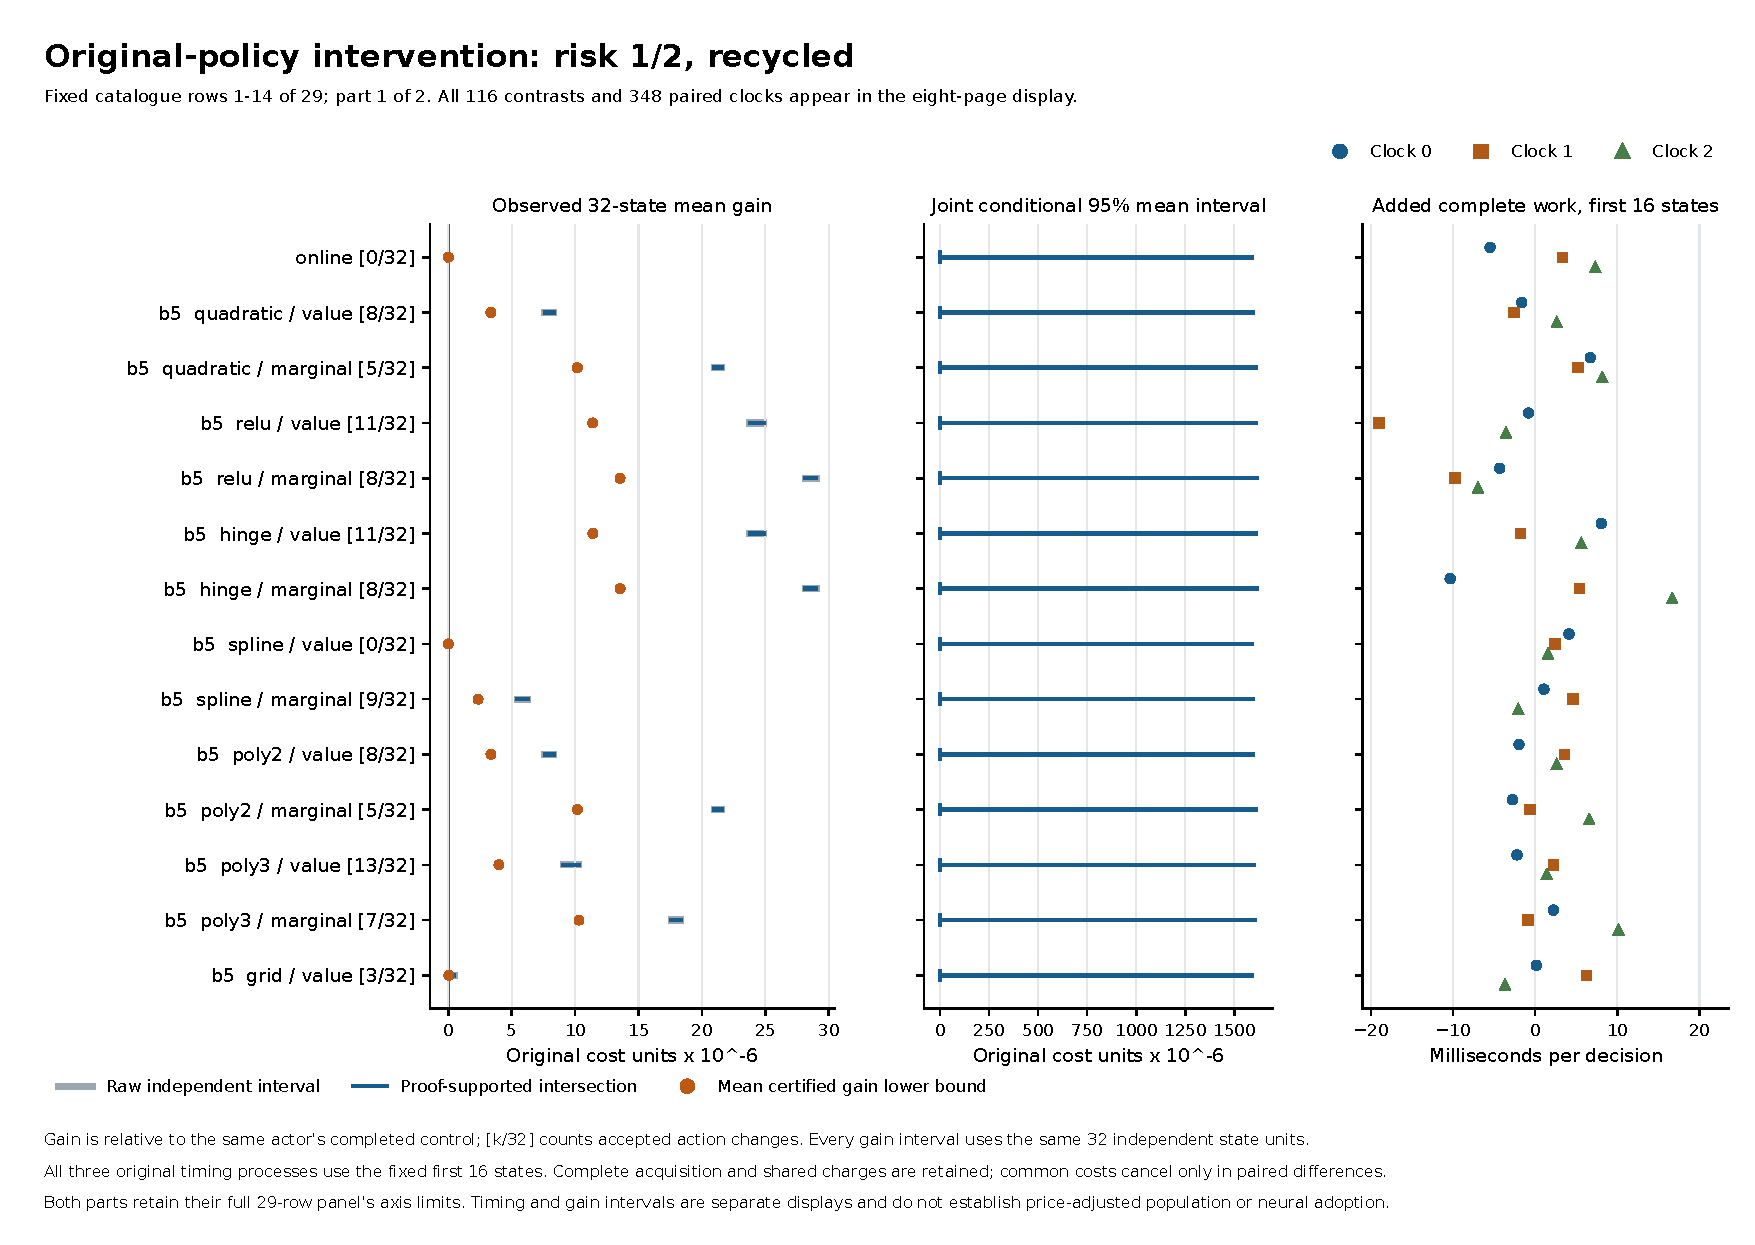
\includepdf[pages=-,fitpaper=true,pagecommand={\thispagestyle{empty}}]{figures122/runtime03-display/complete_catalogue_display122.pdf}
\clearpage
\endgroup


\section{Retained complete R121 main-article account}
\label{dev:main121}
The following introduction, completed numerical account and discussion retain
R121's own states, source identities, failed attempts and negative findings.
The R121 marginal statements and complete proofs remain in the technical
supplement. Historical words such as ``current'' retain their original date.
\section{Introduction}
\label{sec:introduction121}

A dynamic decision maker buys an approximation because it changes the cost of
making a good decision. In a constrained investment problem, an accurate
continuation level can still give the wrong incentive to invest, while a
continuation with a large common level error can choose the correct action.
Under recursive risk, the difficulty is greater: changing a continuation can
also change which shocks receive adverse weight. A numerical method must
therefore connect its acquired information, its fitted critic, its feasible
actor and its computational work to the original recursive objective.

Neural Bellman Operators (NBOs) address this chain by constructing and learning
recursive continuation operators together with an account of their policy
error. The object is the Bellman operator of the specified economy. Its
criterion, information filtration, constraints and boundary conditions remain
part of that object throughout approximation and deployment. The paper retains
both a constructive own-future neural operator and an analysis of arbitrary
acquired critics. It develops their links with stochastic control and, under
separate explicit assumptions, nonlinear Brownian recursive utility. A result
for the nested risk investment application is not automatically a welfare
improvement in a different expected-utility or nonlinear recursive-utility
model.

The central computational question is which continuation information is worth
acquiring. Earlier NBO calculations found a concrete mismatch: every
certificate-oriented fit in a retained comparison reduced a residual-span
criterion, but the aggregate number of rejected first actions increased from
644 to 757. The quadratic control remained a strong complete-service baseline.
The subsequent policy-comparison calculations preserved that economic
criterion and constructed safe actual improvements, yet acquisition still
used a value loss. Those results motivate a new learning calculation in the
original model. Their observations and costs retain their historical
identities in the development companion; the present sample does not reuse
them.

We learn the marginal continuation cost after evaluating the original risk
operator. This order matters. In the two-date investment economy, the original
optimal continuation is the last-date Bellman image of the known terminal
function. It is acquired through paid outward calculations. The root critic
retains the known action cost and learns the action-dependent part of the
integrated continuation. A state-only anchor completes its value level.
The resulting actor is proposed by piecewise minimization of that learned
objective over the original capacity interval. Floating critical-point
calculations generate a proposal; admission requires a certificate for the
original complete policy. The same acquired values, features where relevant, feasible
actions and certification rules are available to the conventional controls.

The mathematical contribution has three connected parts. First, we derive a
continuous original-action marginal and explicit moduli from the nonlinear
investment technology, binding capacity and moving AVaR tails. The central
interval excluded from the adverse tail can touch either shock boundary. Its variational inequalities
control movement of the tail without differentiating a numerical sort or an
unconstrained optimizer. Finite original-risk value enclosures then provide
outward derivative labels, with the precision cost of finite differences paid
explicitly.

Second, a bounded readout is fitted to minimize the worst action-marginal discrepancy over
those outward labels. The finite training problem is convex for each declared
feature family. Exact primal and dual bounds certify the actual stored
coefficients without treating a floating solver's success flag as a proof.
An explicit feature-range construction states how to extend the acquired
information to off-design action comparisons. Its integral along the feasible action path
controls policy loss and possible policy changes; a capacity-sensitive
stationarity bound sharpens the account when available. The argument applies
to a nonconvex fitted polynomial or spline through the all-action comparison,
and never assumes that target smoothness removes a fitted ReLU kink. This
extension is a proved construction whose numerical cell bounds and cost must
also be supplied before it can certify an off-design decision. The current
experiment audits the finite-node fits and admits policies through the
separate original-model certificate; it does not claim to have executed that
global feature-cell calculation.

Third, we state what is lost if the critic's anchor is discarded recursively.
In this very investment transition, a state-dependent continuation level that
does not change a last-date action can shift the root marginal by a known
nonzero amount. A full level-and-contrast recursion therefore carries the
anchor error, the action gap and the future policy error separately. A
noncash-invariant recursive preference receives its own continuation
Lipschitz account. It cannot inherit a monetary shift identity merely because
both criteria have a Bellman notation.

Derivative-assisted economic dynamic programming already uses Hermite
approximation with value and slope information \citep{CaiJudd2015}.
Derivative supervision and task-based model learning also have established
precedents \citep{Czarnecki2017Sobolev,Donti2017Task,ElmachtoubGrigas2022}.
The training certificates use convex duality and affine supporting bounds;
these general tools do not themselves supply a claim of methodological novelty.
The development history also contains certificate-aware readouts and an
action-null quotient analysis. The additional results here concern their
explicit construction and verification for the original recursive risk
operator, including tail changes, paid finite-risk information, feasible
actions and recursive value levels. A three-probe lower bound identifies a
limitation of that stated information interface; it is not a lower bound for
every algorithm with access to the investment formulas.

The numerical comparison changes the learning loss before changing the
evaluation sample. Two separately executed acquisition budgets use nested
state designs. Seven stored representations each have a value-loss and an
action-marginal-loss critic; the online original-model method is included at
both risk levels. Quadratic, polynomial, cubic spline, multilinear grid and
semi-analytic controls form the conventional menu. An exactly corresponding
hinge encoding makes the neural representation claim testable: a geometry
shared with that control is not a uniquely neural contribution.

The protocol fixes 64 new independent initial states, complete original-policy
evaluation, five fresh matched timing processes, exact independent
reconstruction, simultaneous positive and adverse gain inference and full
acquisition/service cost comparisons. It also fixes how unresolved and failed
calculations are retained. The empirical question is whether action-marginal
learning changes decisions, rejections and complete work enough to compensate
for its acquisition cost. A reduction of its own finite-node fitting objective
alone does not answer that question.

The completed comparison gives an adverse answer for the implemented learner.
MARGINAL lowers its independently checked finite-node residual in all 28
loss comparisons, yet its mean original cost is strictly higher in every
independently enclosed 64-state comparison. All 28 simultaneous population
mean-gain intervals contain zero, so the sample conclusion does not establish
a population mean ranking. First rejections increase from 60 under VALUE to
294 under MARGINAL across the stored catalogue, including the matched
encodings. Original-model qualification completes every policy, but does not
remove the adverse mean comparison. MARGINAL is faster in 4 of 28 primary
complete cohorts and slower in 24; all five timing processes and every paid
acquisition remain part of the comparison.

The strong controls matter for the economic conclusion. The online method has
lower independently enclosed sample mean original cost than all 56 learned
cells. At the observed 64-decision volume it also has lower allocated full
cost. Value-fitted splines and polynomials supply additional conventional
cost--accuracy tradeoffs when acquisition is amortized. Every recorded ReLU
scenario has a conventional sample dominator, and all its declared full-menu
price regions are empty, including the upper regions not ruled out by the
intervals. The result leaves a specific computational task: acquire and
control the continuation errors that change feasible actions at less total
cost than the strong method that resolves the original decision directly.
The path and capacity-sensitive bounds state sufficient conditions for that
task; the present experiment does not supply their unexecuted feature-cover
or adaptive-selection costs.

The main article presents the economic operator, its original-risk
qualification and the new learning construction. The supplement contains
complete proofs and retains the earlier action, tail-information and policy
improvement theorems. The development companion preserves the earlier
applications, numerical records, negative findings and source-bound revision
history. This organization keeps the active economic and mathematical
argument readable while retaining the research needed to assess it.

\section{An independent comparison of learning losses}
\label{sec:numerical121}

The completed experiment uses separately committed scientific source and
protocols (F), acquired actors (M), and an independent initial-state sample
(D), in that order.\footnote{The immutable commits begin
\texttt{16bf21334efc}, \texttt{796c5f2badf68} and
\texttt{68eae434c0e6}, respectively. Their complete identities and actual
subprocess receipts are retained in \texttt{RUNS121.json} and the development
companion.} Both acquisition budgets, all actor audits, the primary decisions,
five timing processes, independent original-policy reconstruction and the
fixed statistical calculation were actually executed. The results below use
only these current records; the earlier numerical evidence retains its own
source and execution identity.

\subsection{The original decision and the acquired information}
\label{subsec:design121}

The original model is \eqref{eq:investment95}--\eqref{eq:cost95} at $d=2$,
two dates and risk levels $1/2$ and $3/4$. Investment raises the two next-date
stocks by $a/2$ and $a/4$, whereas the continuous innovation shifts them by
$(z,-z)$. It therefore changes the stocks' imbalance without changing their
aggregate. The decision trades the current adjustment cost against tracking,
the low-stock penalty, capacity and the original risk-sensitive continuation.
All objective quantities below use the original normalized cost units; the
experiment has no monetary or consumption-equivalent calibration.

Two endpoint state grids have
$5^2$ and $9^2$ states. Each buys five normalized-action derivative contexts
and their fixed feasible probes, or thirteen original-value contexts per
state. The protocol requires a separate actual acquisition process for each
budget. Every method
within it receives the same complete information bundle and is charged for
its declared standalone acquisition. The optimized last-date continuation is
acquired from the original known terminal primitives. It is neither a free
oracle nor a target supplied by another representation. The root critic learns
the original integrated continuation difference; its separately stored
state-only anchor completes the value level. The future deployed controller
is unchanged, with $\beta 2^{-20}$ charged once in a complete-policy upper
bound.

\subsection{Representations, losses and the complete decision service}
\label{subsec:methods121}

The seven stored families are a convex quadratic, an anchored ReLU critic,
its exactly corresponding conventional hinge encoding, a tensor cubic
spline, unrestricted polynomials of degrees two and three, and a multilinear
grid. The VALUE and MARGINAL fits use the same coefficient box and features
within a family. VALUE uses every paid value, including the probes. MARGINAL
uses the outward original-action labels. The online baseline computes its
proposal directly from the original model. Every proposal faces the same
complete original-law certificate, refusal, conventional fallback,
integration refinement and rational totalization.

\begin{table}[t]
\centering\small
\caption{Declared learned continuation representations. Counts are the stored
readout coefficients at budgets 5 and 9. Every family receives the same paid
information within a budget; the two losses face the same family and box.}
\label{tab:representations121}
\begin{tabular}{p{0.18\textwidth}p{0.60\textwidth}r}
\toprule
Family & Anchored representation and restriction & Counts\\
\midrule
Quadratic & $v,x_0v,x_1v,v^2$; nonnegative $v^2$ coefficient & $4/4$\\
Polynomial 2 & The same monomials with signed coefficients & $4/4$\\
Polynomial 3 & Total degree at most three; every monomial contains $v$ & $10/10$\\
ReLU & Three base features and 36 fixed anchored hinges; nonnegative nonlinear readouts & $39/39$\\
Hinge & The exact same features and readout, independently encoded in a coordinate loop & $39/39$\\
Cubic spline & Tensor clamped cubic basis; anchored action-axis restriction & $48/100$\\
Linear grid & Tensor linear hats on the actual state and action grids & $100/324$\\
\bottomrule
\end{tabular}
\end{table}

All signed coefficients lie in $[-128,128]$; the stated nonnegative ones lie
in $[0,128]$. The hidden ReLU directions are fixed before acquisition and
are not selected using held-out outcomes. Stored readouts use 30-bit dyadic
rounding. The independently reconstructed finite-box optimization gap applies
to these actual coefficients. It does not assert that a floating optimizer
returned the exact mathematical minimizer. The matched hinge is not an
independent fit; it pays the complete corresponding ReLU phase as well as
its own encoding, identity check and audit.

The learned proposal enumerates the declared action pieces, endpoints and
computed real critical points. Numerical root enumeration proposes an action;
the original economic certificate decides whether to deploy it. A rejected
first proposal remains an outcome of the learning method even when a later
conventional fallback completes the decision. The online control uses a
512-midpoint, 24-iteration original-root proposal. Every completed policy must
meet the original regret target $1/256$ and interval-width target $1/8192$.
Thus a method cannot compensate for an inaccurate actor by silently relaxing
the economic accuracy requirement.

\subsection{Independent reconstruction and the statistical unit}
\label{subsec:validationdesign121}

The source/protocol commit precedes all acquisition. The acquired model
commit precedes a single new operating-system entropy draw. The state commit
precedes every outcome. There are 58 policy cells, 3,712 primary singleton
decisions and 9,280 decisions in five serial fresh timing processes. The
independent economic reconstruction evaluates all distinct final-policy and
raw-proposal keys with the same rational design, and the separate training
audit reconstructs the actual algebraic feature rows and finite-box gaps.
The 64 states, rather than risk cells or repeated clocks, are the independent
statistical units. Their population is the product uniform law on the two
40-bit initial-state coordinates, conditional on the stated independent
OS-entropy assumption. The original innovation distribution remains
continuous. Independent validation reconstructs optimized-continuation values
with exact rational primitive formulas and adds the implemented-future
allowance once; compatibility with a production interval does not by itself
certify that interval's narrower endpoints.

Gain is original cost under VALUE minus original cost under MARGINAL on the
same state. It can have either sign. Both completed policies have regret in
$[0,1/256]$, so a paired gain lies in $[-1/256,1/256]$. The fixed joint
95 percent family in Proposition~\ref{prop:jointinference121} includes the
two optimal-value means, all 58 policy-regret means, all 28 signed loss
contrasts, 112 signed threshold probabilities and both endpoints of all 58
first-rejection probabilities. Identical policy keys cancel exactly without
creating new sample units. Raw proposals have no final-service regret cap;
their complete sample diagnostics are reported separately. Cross-family
sample comparisons and compute-price regions do not acquire an undeclared
population-superiority interpretation.

The complete prospective design and reporting family are
retained in \texttt{PROTOCOL121.md}, \texttt{INDEPENDENT\_PROTOCOL121.md} and
\texttt{REPORTING\_SPEC121.md}.

\section{Learning the original action marginal: completed evidence}\label{sec:results121}

The experiment changes the fitted original Bellman critic. VALUE and MARGINAL use the same paid original-law value probes, the same anchored features, coefficient boxes and feasible proposal rule within each budget. MARGINAL is fitted to minimize the finite-node robust action-marginal loss; VALUE is fitted to minimize bounded value least squares. Both fitting calculations retain their actual independently bounded optimization gaps. The trained critic proposes an action, and the unchanged original-model service qualifies the complete policy. Thus a smaller training loss and a better original economic decision are distinct outcomes.

All 56 stored actors and the online comparator were fixed before the new 64-row initial-state sample. The completed study contains all 58 risk--policy cells, 3,712 primary decisions and 9,280 decisions in five fresh serial timing processes. Both risks share the same 64 initial states; neither timing repeats nor the equal-feature hinge encoding increase the number of independent observations. The innovation distribution remains continuous and the original future controller is unchanged.

The independent primitive implementation evaluated 1,301 distinct exact state--action--risk keys, including every available first proposal and every final policy, using 167,829 terminal contexts. Its fixed 64-cell enclosures reconstruct original optimized-continuation values and add the unchanged $\beta 2^{-20}$ future-policy allowance once. Agreement with production intervals is compatibility; it does not certify the production compiler's narrower endpoints. All final production policies qualified at regret target $1/256$ and interval-width target $1/8192$. The largest saved production regret upper bound was 0.0038604, and the largest recorded interval width was 0.00000286.

\subsection{Original economic gains and the cost of qualification}\label{subsec:learninggains121}

Of the 28 prespecified MARGINAL-minus-VALUE treatments, independently enclosed gain $J_{\rm V}-J_{\rm M}$ was strictly positive in 0, strictly negative in 28, exactly zero in 0, and contained zero in 0 complete-sample comparisons. Actual final actions differed in 889 of the 1,792 paired state records. Under the fixed joint 95 percent population family, 0 mean-gain lower bounds were positive, 0 mean-gain upper bounds were negative, 0 intervals were exactly zero and 28 contained zero. These are signed learning treatments: they do not inherit the nonnegative safe-gain restriction of the older post-fit R120 intervention.

Table~\ref{tab:learninggains121} reports every treatment. Gain intervals are outward decimal displays of exact rational record arithmetic. A positive gain denotes lower original cost under MARGINAL. The population column uses only the 64 initial-state units and the prospectively fixed simultaneous family; it is not a confidence interval for runtime or for superiority over the entire representation menu.

\begingroup
\small\setlength{\tabcolsep}{3pt}
\begin{longtable}{rrlrrrrr}
\caption{All learning contrasts. Sample gain is in $10^{-6}$ original objective units; population gain is in $10^{-3}$ units. $\Delta R$ is MARGINAL minus VALUE first rejections. $T$ ratios compare MARGINAL with VALUE for the complete cohort; the five-clock column is their descriptive median, with every clock retained in the development tables.}\label{tab:learninggains121}\\
\toprule
$\alpha$ & Grid & Family & Sample $10^6G$ & Population $10^3G$ & $\Delta R$ & $T_{64}$ & Med. $T_{32}$\\
\midrule\endfirsthead
\toprule
$\alpha$ & Grid & Family & Sample $10^6G$ & Population $10^3G$ & $\Delta R$ & $T_{64}$ & Med. $T_{32}$\\
\midrule\endhead
\midrule\multicolumn{8}{r}{Continued on next page}\\\endfoot
\bottomrule\endlastfoot
$1/2$ & 5 & Quad. & $[-81.34,-79.30]$ & $[-2.218,2.057]$ & 17 & 1.449 & 1.560\\
$1/2$ & 5 & ReLU & $[-111.21,-109.48]$ & $[-2.248,2.027]$ & -1 & 0.923 & 0.959\\
$1/2$ & 5 & Hinge & $[-111.21,-109.48]$ & $[-2.248,2.027]$ & -1 & 1.015 & 0.946\\
$1/2$ & 5 & Spline & $[-77.93,-75.94]$ & $[-2.215,2.061]$ & 0 & 0.902 & 0.975\\
$1/2$ & 5 & Poly2 & $[-81.34,-79.30]$ & $[-2.218,2.057]$ & 17 & 1.624 & 1.540\\
$1/2$ & 5 & Poly3 & $[-227.61,-225.34]$ & $[-2.364,1.911]$ & 17 & 1.788 & 1.653\\
$1/2$ & 5 & Grid & $[-186.16,-184.27]$ & $[-2.323,1.952]$ & 0 & 1.026 & 1.015\\
$1/2$ & 9 & Quad. & $[-122.55,-120.53]$ & $[-2.259,2.016]$ & 17 & 1.684 & 1.378\\
$1/2$ & 9 & ReLU & $[-70.56,-68.80]$ & $[-2.207,2.068]$ & 10 & 1.165 & 1.126\\
$1/2$ & 9 & Hinge & $[-70.56,-68.80]$ & $[-2.207,2.068]$ & 10 & 1.029 & 1.043\\
$1/2$ & 9 & Spline & $[-48.19,-46.39]$ & $[-2.185,2.090]$ & 0 & 0.948 & 0.983\\
$1/2$ & 9 & Poly2 & $[-122.55,-120.53]$ & $[-2.259,2.016]$ & 17 & 1.617 & 1.562\\
$1/2$ & 9 & Poly3 & $[-360.72,-358.53]$ & $[-2.497,1.778]$ & 18 & 1.492 & 1.422\\
$1/2$ & 9 & Grid & $[-177.12,-175.16]$ & $[-2.314,1.962]$ & 0 & 1.051 & 1.020\\
$3/4$ & 5 & Quad. & $[-24.26,-22.17]$ & $[-2.161,2.115]$ & 17 & 1.226 & 1.587\\
$3/4$ & 5 & ReLU & $[-98.48,-96.37]$ & $[-2.235,2.040]$ & 2 & 1.179 & 0.970\\
$3/4$ & 5 & Hinge & $[-98.48,-96.37]$ & $[-2.235,2.040]$ & 2 & 1.042 & 0.883\\
$3/4$ & 5 & Spline & $[-67.12,-64.89]$ & $[-2.204,2.072]$ & 0 & 0.999 & 1.038\\
$3/4$ & 5 & Poly2 & $[-24.26,-22.17]$ & $[-2.161,2.115]$ & 17 & 1.891 & 1.552\\
$3/4$ & 5 & Poly3 & $[-303.29,-300.90]$ & $[-2.440,1.836]$ & 13 & 1.360 & 1.289\\
$3/4$ & 5 & Grid & $[-190.99,-188.94]$ & $[-2.328,1.948]$ & 0 & 1.065 & 0.981\\
$3/4$ & 9 & Quad. & $[-114.37,-112.13]$ & $[-2.251,2.025]$ & 16 & 1.559 & 1.596\\
$3/4$ & 9 & ReLU & $[-152.83,-150.96]$ & $[-2.290,1.986]$ & 6 & 1.077 & 0.982\\
$3/4$ & 9 & Hinge & $[-152.83,-150.96]$ & $[-2.290,1.986]$ & 6 & 1.062 & 1.093\\
$3/4$ & 9 & Spline & $[-69.18,-67.19]$ & $[-2.206,2.070]$ & 0 & 1.074 & 0.958\\
$3/4$ & 9 & Poly2 & $[-114.37,-112.13]$ & $[-2.251,2.025]$ & 16 & 1.667 & 1.635\\
$3/4$ & 9 & Poly3 & $[-318.24,-315.71]$ & $[-2.455,1.821]$ & 18 & 1.627 & 1.563\\
$3/4$ & 9 & Grid & $[-245.78,-243.82]$ & $[-2.383,1.893]$ & 0 & 1.003 & 1.062\\
\end{longtable}
\endgroup


Across the full primary catalogue, 354 first proposals were not accepted, 354 available first actions changed before deployment, 0 numerical service failures were retained and 0 exact fallbacks were used. There were 0 unavailable raw proposals and 4,066 saved qualification attempts, of which 354 did not qualify. Every attempted action and its paid work remain recorded. A final qualifying action does not retroactively qualify a rejected raw action.

The independent evaluator reports original objective, optimum and regret intervals for each final policy and available raw proposal. Squared action error is bounded using the original curvature, and the reported RMS quantity is an upper bound, not an observed exact action error. A raw-proposal cell aggregate is unavailable if any raw proposal is absent. Complete independent regret intervals are retained alongside their intersection with the separately proved final-service regret cap; the fixed statistical program states which interval it uses.

\subsection{What the learning calculation certifies}\label{subsec:fitresults121}

The exact independent finite-design audit found a smaller stored-coefficient marginal residual for MARGINAL in 28 of the 28 treatments, equality in 0, and a larger residual in 0. It reconstructs the feature and derivative design with rational arithmetic, checks the 30-bit coefficients and boxes, and bounds the finite-box optimum using valid rational dual weights. The marginal optimality-gap upper bounds range from 0.0000000 to 0.0000001; the corresponding VALUE least-squares gap upper bounds range from 0.0000000 to 0.0002331. The complete per-model results include floating-design discrepancies and both losses evaluated at every actual stored coefficient vector.

These finite-node optimization statements establish the implemented fitting calculation. A global feature-cover bound was not numerically established by this experiment, and a small node residual is not a substitute for the separate original-law policy certificate. The two grids measure paid information and feature-budget changes within this two-state, two-date economy. They do not provide state-dimension, horizon or innovation-dimension scaling evidence.

The ReLU and hinge controls have identical fixed features and stored readouts. In the primary records, 512 of 512 paired final actions and 512 paired raw proposals were identical. All five timing comparisons are retained separately. Hinge pays the corresponding full ReLU fitting charge plus its own identity, encoding and audit costs. It is a conventional equal-feature control, not an independent fit or an additional independent scientific outcome; shared geometry cannot establish a neural-exclusive representation advantage.

\subsection{Full paid comparisons and conditional use}\label{subsec:costresults121}

MARGINAL had a lower complete-cohort primary clock in 4 of 28 treatments and a higher clock in 24. Among all 140 matched repeated clocks, it was faster in 40 and slower in 100; the complete-cohort ratios ranged from 0.790 to 1.903. When acquisition and the declared process overhead are included at the measured cohort size, the five-clock comparisons contain 38 lower-cost and 102 higher-cost MARGINAL records. These repeated observations describe the recorded hardware circumstances and are not runtime confidence bounds.

Each learned method pays the complete shared risk-label bundle, its own complete fit and serialization phase, the corresponding required exact training audit, and the explicitly allocated common process residual. Hinge also pays its parent ReLU phase and parent training audit. Competitors' fits and the other risk's labels are not charged as information used by that method. Each service clock includes loading, original-law certification, rejected candidates, refinement and fallback; event serialization is already inside these measured clocks and is not added again. These component sums are declared standalone allocations of actual measurements, not separately observed one-model processes.

The selected acquisition, training-audit, primary-with-five-timings, independent-validation and statistical subprocess receipts total 3455.197 seconds. The independent original-policy evaluator contributes 2598.580 seconds of that research cost. Failed frozen-source scientific attempts number 0, with 0.000 additional seconds retained in the whole-study ledger. Reporting, typesetting, publication and remote waits have their own receipts and are outside these selected scientific clocks. The nested timing children are already inside the primary outer clock and are not added twice.

For the prespecified reuse volumes $N\in\{64,256,1024,16384\}$, the deployment scenario is $C_m(N)=A_m+H_m+L_m+(N/n)(T_m-L_m)$. Here $A_m$ is the allocated acquisition and training-audit cost, $H_m$ the stated common process residual, $L_m$ the cold load, and $T_m$ the measured complete cohort. The primary scenario has $n=64$ and matching 64-state economics; each timing scenario has $n=32$ and matching first-32 economics. Independent all-policy research validation is reported separately and excluded from this deployment-reuse formula. Reuse is a specified amortization calculation, not measured throughput.

For every conventional rival, the criterion is $N J_m+p C_m(N)$ with $p\geq0$ in original objective units per measured second. A sufficient price domain requires the lower original-gain bound minus $p$ times the extra cost to be strictly positive. The upper domain is only a pairwise condition not ruled out by these intervals. The machine tables preserve all full-menu and within-budget rivals, empty domains, reversed cost inequalities and strict endpoints.

For the eight ReLU risk--budget--loss cells and four volumes, the primary64 comparisons yield 0 nonempty sufficient regions and 0 nonempty upper regions among 32 full-menu scenarios. The 160 individual timing scenarios yield 0 nonempty sufficient and 0 nonempty upper regions. Intersecting all five clocks at a common price leaves 0 nonempty sufficient and 0 nonempty upper regions among 32 cases. An empty five-clock intersection does not state that every individual-clock region is empty. A nonempty upper intersection neither establishes joint attainability nor justifies adoption or population superiority.

All 58 cells, all conventional wins and losses, all 28 learning and 28 budget contrasts, the full pairwise recorded-menu comparisons, the 348 distinct cohort clocks and all 1,392 cost/frontier rows remain in the development and machine tables. Methods whose original-objective and paid-cost intervals leave an unresolved choice remain unresolved.


\subsection{Economic interpretation under the original criterion}
\label{subsec:interpretation121}

The adverse mean gains concern the deployed decisions in the same investment
economy. The relevant incentive combines the known marginal adjustment cost
$h'(a)$ with the original risk-integrated continuation marginal. Correct
boundary signs can justify no investment or a capacity action; an interior
decision needs their balance at the chosen state and action. Minimizing the
largest discrepancy at the acquired nodes does not by itself control that
balance off design or the integrated contrast between competing actions.
Theorem~\ref{thm:quotientlearning121} and
Proposition~\ref{prop:marginalpolicy121} make those additional requirements
explicit. The campaign has not isolated how much of the adverse performance
comes from label width, the allocation of approximation error across nodes,
or the fitted geometry away from them. Assigning the outcome to any one of
these mechanisms would require a further independently specified comparison.

The refusal records show a direct consequence for the decision service.
Across the two risks and budgets, VALUE incurs 60 first rejections and
MARGINAL incurs 294, out of 1,792 proposals each. These are catalogue counts;
matched hinge policies do not add independent observations. Every one of the
354 refusals triggers a paid conventional fallback and changes the deployed
action. The final adverse mean gains in Table~\ref{tab:learninggains121}
already include that correction. Thus qualification protects the declared
policy-loss ceiling while leaving substantial differences in attained
economic accuracy and total work. The original-action RMS quantities in
Table~\ref{tab:allpolicies121} remain upper bounds inferred from curvature,
not exact measured action errors.

The online original-model control has a strictly lower independently enclosed
64-state mean cost than each of the 56 learned cells in the saved paired
comparisons. Its mean regret upper bounds are $1.88\times10^{-6}$ and
$2.04\times10^{-6}$ at risk levels $1/2$ and $3/4$. A strong conventional
approximation can get much closer to that accuracy than the tested neural
critic. At budget 9, VALUE spline mean regret lies in
$[1.10,3.29]\times10^{-6}$ and $[4.61,7.08]\times10^{-6}$ at the two risks;
MARGINAL ReLU regret lies in $[381.99,384.17]\times10^{-6}$ and
$[470.95,473.34]\times10^{-6}$. These are outward sample enclosures under
the original criterion. They are neither welfare estimates for another
preference model nor population rankings across representations.

Acquisition changes the economically relevant cost comparison. At $N=64$,
the online control's allocated complete costs are 10.108 and 10.846 seconds,
below every learned alternative at the corresponding risk. Amortization can
make conventional approximation useful at larger declared reuse volumes.
For example, at $N=16384$ the coarse VALUE spline costs 510.208 and 470.272
seconds in the primary-clock scenario, against 1193.379 and 1382.227 for the
online method, while retaining a higher original sample cost. These are
calculations under the stated reuse formula, not observed throughput. Their
economic relevance depends on the price of computation and the accepted
accuracy tradeoff. The entire conventional menu, every clock and all four
volumes enter the price tests; a favorable comparison with a selected rival
does not establish adoption against that menu. Each of the 192 ReLU
primary-or-individual-clock volume scenarios has a conventional sample
dominator in the saved cost-frontier table.

The larger acquisition budget is also not a monotone policy improvement.
It buys $81/25$ times as many original-value contexts per risk, with allocated
acquisition and audit charges about 2.53--2.77 times as large. Of the 28
fine-versus-coarse sample contrasts, 15 favor the finer budget, 12 favor the
coarser budget and one remains unresolved. MARGINAL ReLU improves at risk
$1/2$ but worsens at risk $3/4$; its first rejections respectively rise from
10 to 14 and fall from 13 to 10. Table~\ref{tab:budgetscaling121} retains
all contrasts. These changes show why neither denser acquisition nor a
lower refusal count can replace direct measurement of original economic
loss. They concern two information budgets in the same economy, with no
state-dimension or horizon extrapolation.

Statewise outcomes vary within the adverse mean comparison.
At the prespecified threshold $2^{-20}$, the fixed joint 95 percent event
family gives positive lower bounds on the probability of a benefit in
26 of 28 treatments and of harm in all 28. At threshold $2^{-16}$ the
corresponding counts are 25 and 28. These separate event statements coexist
with unresolved population mean gains. The independent comparisons were
not used to select the deployed actions. A deployable rule that chooses a
statewise improvement must acquire valid original-objective contrast bounds
before making that choice and pay for them, as required by
Theorem~\ref{thm:quotientlearning121}. No gain, service cost or adoption
region is credited to such an unexecuted selector.

\section{Economic use and the remaining research task}
\label{sec:discussion121}

The role of a Neural Bellman Operator is to acquire and reuse continuation
information that changes feasible economic decisions at an acceptable total
cost. The new construction supplies original-marginal regularity, paid
derivative labels, checked finite-box fitting gaps and sufficient action
conditions under the original recursive risk objective. The implemented
MARGINAL learner nevertheless raises the independently enclosed sample mean
cost in every loss comparison, and its timing improvements are a minority of
the complete records. This campaign has not established the intended neural
economic or computational advantage. The research objective remains a
competitive learned recursive Bellman operator, with the original model,
strong controls and full decision costs determining that comparison.

The action bounds specify a concrete route for further algorithmic work.
An original derivative enclosure can stop regret certification when its
capacity-sensitive bound plus the future-policy allowance meets the economic
tolerance. A proposed policy change requires the original continuation
contrast bound, including that allowance, to certify improvement. Building
these bounds from the learned critic requires the feature-range and
off-design calculations in Theorem~\ref{thm:quotientlearning121}; the current
finite-node fitting audit does not provide them. The simultaneous event
results preserve both potential gains and harms across states, but they do
not implement a selection rule. Using independent evaluation labels to
choose the favorable actions afterwards would give the selector information
and cost treatment absent from the frozen experiment.

Precision allocation must therefore be tied to a decision that the additional
information can resolve. Taking closer finite-difference probes while leaving
the value enclosures unchanged can amplify uncertainty through division by
the probe distance. Increasing the state grid also costs more without
guaranteeing a better feasible action, as the complete budget comparison
shows. The proved path and stationarity conditions identify valid stopping
tests; the cost of acquiring them, the choice of refinement and a safe
deployable selector remain to be demonstrated under a new independent
protocol. The existing probe radius, grids, models and evaluation states
are unchanged by this interpretation. Risk integration and the
state-dependent anchor remain essential when an operator is used recursively.

The acquisition budgets in this experiment change information density and
representation size within the same two-state economy. They do not establish
scalability in horizon, state dimension or innovation dimension. The retained
theorems describe those separate objects and their assumptions; their
historical experiments and unresolved regions remain in the development
companion. The stopping, accuracy-allocation and risk-information questions
therefore remain part of the NBO programme under the original economic
criteria.

A neural-specific advantage requires a distinction that a conventional
method with the same information, features, feasible policies and resources
cannot reproduce. The exactly matched hinge control makes one such boundary
explicit. Conditional adoption additionally requires the original objective
gain to pay for all acquisition and complete-service work at a stated price
and volume. These are empirical and mathematical requirements for an
economically useful NBO, not consequences of a successful optimization status
or a smaller internal loss.

The measured ReLU--hinge comparison needs a further computational distinction.
The two encodings carry identical mathematical features and readouts. Under
the frozen acquisition procedure, the coordinate-loop hinge implementation
pays for the corresponding ReLU fit and its own encoding, identity check and
audit. Those are real costs of the executed implementation, and remain in the
ledger. A conventional hinge representation can also use the same batched
evaluation and elementary operations as the ReLU implementation. Consequently
a cost difference caused by the declared copy or evaluation procedure cannot
establish a neural-specific computational advantage. Any sufficient price
region against the recorded implementations is conditional on that measured
menu. Its interpretation must also retain the other strong conventional
alternatives and the distinction between implementation cost and a limitation
of conventional representation.

\section{R121 author revision and the source-bound research record}
\label{dev:custody121}
The complete preceding author manuscript is R120 at source commit
\nolinkurl{39a20bf1fe011175857811bf67bacd788ae80c52}, package commit
\nolinkurl{cc58ec9613044f97aa1ae5c8d60ec1c3c0021dcd} and final receipt commit
\nolinkurl{f06f220aea525088e82228e8e9be4947fb81b1ca}. Its actual successful
source CI and all package bytes have been read back independently for this
revision. The controlling persisted advisory remains R97 at
\nolinkurl{9723c6cd2cc8b3e071422f3e522d4a843946db63}; it reviewed its own
specified R97 manuscript, not the R120 or R121 results. It is an
owner-commissioned AI advisory, not an Econometric Society editorial decision.
The author revision retains the NBO research identity and Econometrica goal.

The present source, acquired actors, independent sample, original-model
executions, validation, manuscript PDFs and package have distinct identities.
R98, R115 and other separately frozen historical experiments retain their own
uncompleted or completed status. A result in R121 cannot complete them.
The preservation map binds all 35 original report bodies and the inherited
request routes, source files and historical evidence. An archived assertion
is preserved with its correction history; preservation is not a fresh claim
that an unsupported earlier assertion has been proved.
\section{Complete R121 numerical tables}\label{sec:developmentresults121}

These tables are deterministic displays of completed, hash-bound records. V and M denote VALUE and MARGINAL; O denotes the online original-model comparator. Every risk and method is retained. Interval endpoints are rounded outward; clocks are descriptive rounded displays. Exact rational numbers, all row-level observations and all conditional price endpoints remain in the machine tables.

\subsection{All original policy levels and action bounds}

\begingroup
\small\setlength{\tabcolsep}{3pt}
\begin{longtable}{rrlrrrrr}
\caption{All 58 complete policy cells, each with 64 independent initial-state rows. Original regret is the independently reconstructed interval in $10^{-6}$ units before any use of the production cap. RMS is an upper bound on original action error. Reject counts retain the first proposal, and changed counts compare every available raw proposal with the final action.}\label{tab:allpolicies121}\\
\toprule
$\alpha$ & Grid & Policy & Mean original $J$ & $10^6$ regret & RMS bound & Reject & Changed\\
\midrule\endfirsthead
\toprule
$\alpha$ & Grid & Policy & Mean original $J$ & $10^6$ regret & RMS bound & Reject & Changed\\
\midrule\endhead
\midrule\multicolumn{8}{r}{Continued on next page}\\\endfoot
\bottomrule\endlastfoot
$1/2$ & 0 & Online O & $[0.631682,0.631685]$ & $[0.00,1.88]$ & 0.001371 & 0 & 0\\
$1/2$ & 5 & Quad. V & $[0.631812,0.631815]$ & $[130.07,132.45]$ & 0.011509 & 0 & 0\\
$1/2$ & 5 & Quad. M & $[0.631893,0.631896]$ & $[210.63,212.76]$ & 0.014587 & 17 & 17\\
$1/2$ & 5 & ReLU V & $[0.631974,0.631977]$ & $[291.39,293.65]$ & 0.017136 & 11 & 11\\
$1/2$ & 5 & ReLU M & $[0.632084,0.632087]$ & $[401.78,403.98]$ & 0.020100 & 10 & 10\\
$1/2$ & 5 & Hinge V & $[0.631974,0.631977]$ & $[291.39,293.65]$ & 0.017136 & 11 & 11\\
$1/2$ & 5 & Hinge M & $[0.632084,0.632087]$ & $[401.78,403.98]$ & 0.020100 & 10 & 10\\
$1/2$ & 5 & Spline V & $[0.631686,0.631689]$ & $[3.98,6.33]$ & 0.002516 & 0 & 0\\
$1/2$ & 5 & Spline M & $[0.631763,0.631766]$ & $[80.85,83.25]$ & 0.009125 & 0 & 0\\
$1/2$ & 5 & Poly2 V & $[0.631812,0.631815]$ & $[130.07,132.45]$ & 0.011509 & 0 & 0\\
$1/2$ & 5 & Poly2 M & $[0.631893,0.631896]$ & $[210.63,212.76]$ & 0.014587 & 17 & 17\\
$1/2$ & 5 & Poly3 V & $[0.631812,0.631815]$ & $[129.68,132.14]$ & 0.011495 & 0 & 0\\
$1/2$ & 5 & Poly3 M & $[0.632039,0.632041]$ & $[356.37,358.58]$ & 0.018937 & 17 & 17\\
$1/2$ & 5 & Grid V & $[0.631699,0.631702]$ & $[16.94,19.27]$ & 0.004389 & 0 & 0\\
$1/2$ & 5 & Grid M & $[0.631884,0.631887]$ & $[202.09,204.45]$ & 0.014299 & 0 & 0\\
$1/2$ & 9 & Quad. V & $[0.631775,0.631778]$ & $[92.29,94.67]$ & 0.009730 & 0 & 0\\
$1/2$ & 9 & Quad. M & $[0.631896,0.631899]$ & $[214.08,216.21]$ & 0.014704 & 17 & 17\\
$1/2$ & 9 & ReLU V & $[0.631994,0.631997]$ & $[312.13,314.50]$ & 0.017735 & 4 & 4\\
$1/2$ & 9 & ReLU M & $[0.632064,0.632067]$ & $[381.99,384.17]$ & 0.019601 & 14 & 14\\
$1/2$ & 9 & Hinge V & $[0.631994,0.631997]$ & $[312.13,314.50]$ & 0.017735 & 4 & 4\\
$1/2$ & 9 & Hinge M & $[0.632064,0.632067]$ & $[381.99,384.17]$ & 0.019601 & 14 & 14\\
$1/2$ & 9 & Spline V & $[0.631683,0.631686]$ & $[1.10,3.29]$ & 0.001812 & 0 & 0\\
$1/2$ & 9 & Spline M & $[0.631731,0.631733]$ & $[48.20,50.59]$ & 0.007113 & 0 & 0\\
$1/2$ & 9 & Poly2 V & $[0.631775,0.631778]$ & $[92.29,94.67]$ & 0.009730 & 0 & 0\\
$1/2$ & 9 & Poly2 M & $[0.631896,0.631899]$ & $[214.08,216.21]$ & 0.014704 & 17 & 17\\
$1/2$ & 9 & Poly3 V & $[0.631766,0.631768]$ & $[83.14,85.52]$ & 0.009248 & 0 & 0\\
$1/2$ & 9 & Poly3 M & $[0.632125,0.632128]$ & $[442.95,445.15]$ & 0.021099 & 18 & 18\\
$1/2$ & 9 & Grid V & $[0.631695,0.631698]$ & $[12.51,14.84]$ & 0.003852 & 0 & 0\\
$1/2$ & 9 & Grid M & $[0.631871,0.631874]$ & $[188.55,190.99]$ & 0.013820 & 0 & 0\\
$3/4$ & 0 & Online O & $[0.640586,0.640589]$ & $[0.00,2.04]$ & 0.001428 & 0 & 0\\
$3/4$ & 5 & Quad. V & $[0.640723,0.640726]$ & $[137.27,139.82]$ & 0.011825 & 0 & 0\\
$3/4$ & 5 & Quad. M & $[0.640747,0.640750]$ & $[160.83,163.07]$ & 0.012770 & 17 & 17\\
$3/4$ & 5 & ReLU V & $[0.640872,0.640875]$ & $[285.60,288.18]$ & 0.016976 & 11 & 11\\
$3/4$ & 5 & ReLU M & $[0.640969,0.640972]$ & $[383.17,385.64]$ & 0.019638 & 13 & 13\\
$3/4$ & 5 & Hinge V & $[0.640872,0.640875]$ & $[285.60,288.18]$ & 0.016976 & 11 & 11\\
$3/4$ & 5 & Hinge M & $[0.640969,0.640972]$ & $[383.17,385.64]$ & 0.019638 & 13 & 13\\
$3/4$ & 5 & Spline V & $[0.640594,0.640597]$ & $[7.49,9.95]$ & 0.003154 & 0 & 0\\
$3/4$ & 5 & Spline M & $[0.640659,0.640663]$ & $[73.27,76.06]$ & 0.008722 & 0 & 0\\
$3/4$ & 5 & Poly2 V & $[0.640723,0.640726]$ & $[137.27,139.82]$ & 0.011825 & 0 & 0\\
$3/4$ & 5 & Poly2 M & $[0.640747,0.640750]$ & $[160.83,163.07]$ & 0.012770 & 17 & 17\\
$3/4$ & 5 & Poly3 V & $[0.640718,0.640721]$ & $[132.12,134.77]$ & 0.011610 & 0 & 0\\
$3/4$ & 5 & Poly3 M & $[0.641020,0.641023]$ & $[434.39,436.90]$ & 0.020902 & 13 & 13\\
$3/4$ & 5 & Grid V & $[0.640608,0.640611]$ & $[21.96,24.47]$ & 0.004946 & 0 & 0\\
$3/4$ & 5 & Grid M & $[0.640798,0.640801]$ & $[211.79,214.49]$ & 0.014646 & 0 & 0\\
$3/4$ & 9 & Quad. V & $[0.640686,0.640689]$ & $[99.74,102.33]$ & 0.010116 & 0 & 0\\
$3/4$ & 9 & Quad. M & $[0.640799,0.640802]$ & $[213.31,215.59]$ & 0.014683 & 16 & 16\\
$3/4$ & 9 & ReLU V & $[0.640905,0.640908]$ & $[318.85,321.44]$ & 0.017929 & 4 & 4\\
$3/4$ & 9 & ReLU M & $[0.641057,0.641060]$ & $[470.95,473.34]$ & 0.021757 & 10 & 10\\
$3/4$ & 9 & Hinge V & $[0.640905,0.640908]$ & $[318.85,321.44]$ & 0.017929 & 4 & 4\\
$3/4$ & 9 & Hinge M & $[0.641057,0.641060]$ & $[470.95,473.34]$ & 0.021757 & 10 & 10\\
$3/4$ & 9 & Spline V & $[0.640591,0.640594]$ & $[4.61,7.08]$ & 0.002661 & 0 & 0\\
$3/4$ & 9 & Spline M & $[0.640659,0.640662]$ & $[72.63,75.27]$ & 0.008676 & 0 & 0\\
$3/4$ & 9 & Poly2 V & $[0.640686,0.640689]$ & $[99.74,102.33]$ & 0.010116 & 0 & 0\\
$3/4$ & 9 & Poly2 M & $[0.640799,0.640802]$ & $[213.31,215.59]$ & 0.014683 & 16 & 16\\
$3/4$ & 9 & Poly3 V & $[0.640680,0.640683]$ & $[93.66,96.37]$ & 0.009817 & 0 & 0\\
$3/4$ & 9 & Poly3 M & $[0.640997,0.641000]$ & $[410.87,413.35]$ & 0.020331 & 18 & 18\\
$3/4$ & 9 & Grid V & $[0.640601,0.640604]$ & $[15.08,17.60]$ & 0.004195 & 0 & 0\\
$3/4$ & 9 & Grid M & $[0.640846,0.640849]$ & $[259.81,262.38]$ & 0.016199 & 0 & 0\\
\end{longtable}
\endgroup


\begingroup
\small\setlength{\tabcolsep}{3pt}
\begin{longtable}{rrlrrrrr}
\caption{All first-proposal outcomes and completion work. Raw proposals have no final qualification guarantee; an aggregate with any unavailable raw proposal is explicitly unavailable. Every unique available raw action, including rejections, was independently evaluated.}\label{tab:rawproposals121}\\
\toprule
$\alpha$ & Grid & Policy & Raw mean $J$ & Raw $10^6$ regret & Missing & Exact & Attempts\\
\midrule\endfirsthead
\toprule
$\alpha$ & Grid & Policy & Raw mean $J$ & Raw $10^6$ regret & Missing & Exact & Attempts\\
\midrule\endhead
\midrule\multicolumn{8}{r}{Continued on next page}\\\endfoot
\bottomrule\endlastfoot
$1/2$ & 0 & Online O & $[0.631682,0.631685]$ & $[0.00,1.88]$ & 0 & 0 & 64\\
$1/2$ & 5 & Quad. V & $[0.631812,0.631815]$ & $[130.07,132.45]$ & 0 & 0 & 64\\
$1/2$ & 5 & Quad. M & $[0.633744,0.633747]$ & $[2062.04,2064.47]$ & 0 & 0 & 81\\
$1/2$ & 5 & ReLU V & $[0.632565,0.632568]$ & $[882.32,884.76]$ & 0 & 0 & 75\\
$1/2$ & 5 & ReLU M & $[0.632792,0.632795]$ & $[1109.46,1111.84]$ & 0 & 0 & 74\\
$1/2$ & 5 & Hinge V & $[0.632565,0.632568]$ & $[882.32,884.76]$ & 0 & 0 & 75\\
$1/2$ & 5 & Hinge M & $[0.632792,0.632795]$ & $[1109.46,1111.84]$ & 0 & 0 & 74\\
$1/2$ & 5 & Spline V & $[0.631686,0.631689]$ & $[3.98,6.33]$ & 0 & 0 & 64\\
$1/2$ & 5 & Spline M & $[0.631763,0.631766]$ & $[80.85,83.25]$ & 0 & 0 & 64\\
$1/2$ & 5 & Poly2 V & $[0.631812,0.631815]$ & $[130.07,132.45]$ & 0 & 0 & 64\\
$1/2$ & 5 & Poly2 M & $[0.633744,0.633747]$ & $[2062.04,2064.47]$ & 0 & 0 & 81\\
$1/2$ & 5 & Poly3 V & $[0.631812,0.631815]$ & $[129.68,132.14]$ & 0 & 0 & 64\\
$1/2$ & 5 & Poly3 M & $[0.632784,0.632787]$ & $[1101.86,1104.34]$ & 0 & 0 & 81\\
$1/2$ & 5 & Grid V & $[0.631699,0.631702]$ & $[16.94,19.27]$ & 0 & 0 & 64\\
$1/2$ & 5 & Grid M & $[0.631884,0.631887]$ & $[202.09,204.45]$ & 0 & 0 & 64\\
$1/2$ & 9 & Quad. V & $[0.631775,0.631778]$ & $[92.29,94.67]$ & 0 & 0 & 64\\
$1/2$ & 9 & Quad. M & $[0.633714,0.633717]$ & $[2032.02,2034.45]$ & 0 & 0 & 81\\
$1/2$ & 9 & ReLU V & $[0.632175,0.632177]$ & $[492.15,494.59]$ & 0 & 0 & 68\\
$1/2$ & 9 & ReLU M & $[0.632981,0.632984]$ & $[1298.87,1301.31]$ & 0 & 0 & 78\\
$1/2$ & 9 & Hinge V & $[0.632175,0.632177]$ & $[492.15,494.59]$ & 0 & 0 & 68\\
$1/2$ & 9 & Hinge M & $[0.632981,0.632984]$ & $[1298.87,1301.31]$ & 0 & 0 & 78\\
$1/2$ & 9 & Spline V & $[0.631683,0.631686]$ & $[1.10,3.29]$ & 0 & 0 & 64\\
$1/2$ & 9 & Spline M & $[0.631731,0.631733]$ & $[48.20,50.59]$ & 0 & 0 & 64\\
$1/2$ & 9 & Poly2 V & $[0.631775,0.631778]$ & $[92.29,94.67]$ & 0 & 0 & 64\\
$1/2$ & 9 & Poly2 M & $[0.633714,0.633717]$ & $[2032.02,2034.45]$ & 0 & 0 & 81\\
$1/2$ & 9 & Poly3 V & $[0.631766,0.631768]$ & $[83.14,85.52]$ & 0 & 0 & 64\\
$1/2$ & 9 & Poly3 M & $[0.632908,0.632910]$ & $[1225.04,1227.52]$ & 0 & 0 & 82\\
$1/2$ & 9 & Grid V & $[0.631695,0.631698]$ & $[12.51,14.84]$ & 0 & 0 & 64\\
$1/2$ & 9 & Grid M & $[0.631871,0.631874]$ & $[188.55,190.99]$ & 0 & 0 & 64\\
$3/4$ & 0 & Online O & $[0.640586,0.640589]$ & $[0.00,2.04]$ & 0 & 0 & 64\\
$3/4$ & 5 & Quad. V & $[0.640723,0.640726]$ & $[137.27,139.82]$ & 0 & 0 & 64\\
$3/4$ & 5 & Quad. M & $[0.642646,0.642649]$ & $[2059.33,2062.06]$ & 0 & 0 & 81\\
$3/4$ & 5 & ReLU V & $[0.641487,0.641490]$ & $[900.68,903.40]$ & 0 & 0 & 75\\
$3/4$ & 5 & ReLU M & $[0.641889,0.641893]$ & $[1303.19,1306.03]$ & 0 & 0 & 77\\
$3/4$ & 5 & Hinge V & $[0.641487,0.641490]$ & $[900.68,903.40]$ & 0 & 0 & 75\\
$3/4$ & 5 & Hinge M & $[0.641889,0.641893]$ & $[1303.19,1306.03]$ & 0 & 0 & 77\\
$3/4$ & 5 & Spline V & $[0.640594,0.640597]$ & $[7.49,9.95]$ & 0 & 0 & 64\\
$3/4$ & 5 & Spline M & $[0.640659,0.640663]$ & $[73.27,76.06]$ & 0 & 0 & 64\\
$3/4$ & 5 & Poly2 V & $[0.640723,0.640726]$ & $[137.27,139.82]$ & 0 & 0 & 64\\
$3/4$ & 5 & Poly2 M & $[0.642646,0.642649]$ & $[2059.33,2062.06]$ & 0 & 0 & 81\\
$3/4$ & 5 & Poly3 V & $[0.640718,0.640721]$ & $[132.12,134.77]$ & 0 & 0 & 64\\
$3/4$ & 5 & Poly3 M & $[0.641606,0.641609]$ & $[1019.75,1022.48]$ & 0 & 0 & 77\\
$3/4$ & 5 & Grid V & $[0.640608,0.640611]$ & $[21.96,24.47]$ & 0 & 0 & 64\\
$3/4$ & 5 & Grid M & $[0.640798,0.640801]$ & $[211.79,214.49]$ & 0 & 0 & 64\\
$3/4$ & 9 & Quad. V & $[0.640686,0.640689]$ & $[99.74,102.33]$ & 0 & 0 & 64\\
$3/4$ & 9 & Quad. M & $[0.642431,0.642435]$ & $[1845.25,1848.11]$ & 0 & 0 & 80\\
$3/4$ & 9 & ReLU V & $[0.641080,0.641083]$ & $[493.95,496.60]$ & 0 & 0 & 68\\
$3/4$ & 9 & ReLU M & $[0.641787,0.641790]$ & $[1201.03,1203.76]$ & 0 & 0 & 74\\
$3/4$ & 9 & Hinge V & $[0.641080,0.641083]$ & $[493.95,496.60]$ & 0 & 0 & 68\\
$3/4$ & 9 & Hinge M & $[0.641787,0.641790]$ & $[1201.03,1203.76]$ & 0 & 0 & 74\\
$3/4$ & 9 & Spline V & $[0.640591,0.640594]$ & $[4.61,7.08]$ & 0 & 0 & 64\\
$3/4$ & 9 & Spline M & $[0.640659,0.640662]$ & $[72.63,75.27]$ & 0 & 0 & 64\\
$3/4$ & 9 & Poly2 V & $[0.640686,0.640689]$ & $[99.74,102.33]$ & 0 & 0 & 64\\
$3/4$ & 9 & Poly2 M & $[0.642431,0.642435]$ & $[1845.25,1848.11]$ & 0 & 0 & 80\\
$3/4$ & 9 & Poly3 V & $[0.640680,0.640683]$ & $[93.66,96.37]$ & 0 & 0 & 64\\
$3/4$ & 9 & Poly3 M & $[0.641811,0.641814]$ & $[1224.68,1227.47]$ & 0 & 0 & 82\\
$3/4$ & 9 & Grid V & $[0.640601,0.640604]$ & $[15.08,17.60]$ & 0 & 0 & 64\\
$3/4$ & 9 & Grid M & $[0.640846,0.640849]$ & $[259.81,262.38]$ & 0 & 0 & 64\\
\end{longtable}
\endgroup


\subsection{All finite-design fits and acquisition charges}

\begingroup
\small\setlength{\tabcolsep}{3pt}
\begin{longtable}{rrlrrrrr}
\caption{Every stored model. The marginal residual is the robust finite-node residual at the actual 30-bit coefficients. V-MSE evaluates the VALUE loss on all paid value probes. The gap bounds the optimum of the method's own finite-box fitting problem: least-squares for V, minimax marginal for M. The full charge includes the declared shared information, model phases and required audit; it is not a new isolated process timing.}\label{tab:allfits121}\\
\toprule
$\alpha$ & Grid & Policy & Features & Marg. res. & V-MSE & Own gap & Acq.+audit s\\
\midrule\endfirsthead
\toprule
$\alpha$ & Grid & Policy & Features & Marg. res. & V-MSE & Own gap & Acq.+audit s\\
\midrule\endhead
\midrule\multicolumn{8}{r}{Continued on next page}\\\endfoot
\bottomrule\endlastfoot
$1/2$ & 5 & Quad. V & 4 & 0.69125 & 0.0001680 & 0.0000311 & 13.344\\
$1/2$ & 5 & Quad. M & 4 & 0.32051 & 0.0004681 & 0.0000001 & 13.371\\
$1/2$ & 5 & ReLU V & 39 & 0.49988 & 0.0000792 & 0.0000051 & 14.250\\
$1/2$ & 5 & ReLU M & 39 & 0.26545 & 0.0002430 & 0.0000001 & 13.928\\
$1/2$ & 5 & Hinge V & 39 & 0.49988 & 0.0000792 & 0.0000051 & 14.931\\
$1/2$ & 5 & Hinge M & 39 & 0.26545 & 0.0002430 & 0.0000001 & 14.780\\
$1/2$ & 5 & Spline V & 48 & 0.09537 & 0.0000074 & 0.0000035 & 13.452\\
$1/2$ & 5 & Spline M & 48 & 0.06652 & 0.0000260 & 0.0000001 & 13.530\\
$1/2$ & 5 & Poly2 V & 4 & 0.69125 & 0.0001680 & 0.0000431 & 13.305\\
$1/2$ & 5 & Poly2 M & 4 & 0.32051 & 0.0004681 & 0.0000001 & 13.305\\
$1/2$ & 5 & Poly3 V & 10 & 0.33438 & 0.0000810 & 0.0000893 & 13.460\\
$1/2$ & 5 & Poly3 M & 10 & 0.16595 & 0.0001626 & 0.0000001 & 13.436\\
$1/2$ & 5 & Grid V & 100 & 0.07951 & 0.0000001 & 0.0000001 & 13.613\\
$1/2$ & 5 & Grid M & 100 & 0.07878 & 0.0000302 & 0.0000001 & 13.590\\
$3/4$ & 5 & Quad. V & 4 & 0.68342 & 0.0001671 & 0.0000539 & 14.199\\
$3/4$ & 5 & Quad. M & 4 & 0.31909 & 0.0004664 & 0.0000001 & 14.180\\
$3/4$ & 5 & ReLU V & 39 & 0.49350 & 0.0000792 & 0.0000061 & 14.646\\
$3/4$ & 5 & ReLU M & 39 & 0.26672 & 0.0002642 & 0.0000001 & 14.640\\
$3/4$ & 5 & Hinge V & 39 & 0.49350 & 0.0000792 & 0.0000061 & 15.206\\
$3/4$ & 5 & Hinge M & 39 & 0.26672 & 0.0002642 & 0.0000001 & 15.198\\
$3/4$ & 5 & Spline V & 48 & 0.09768 & 0.0000080 & 0.0000038 & 14.379\\
$3/4$ & 5 & Spline M & 48 & 0.06816 & 0.0000269 & 0.0000001 & 14.361\\
$3/4$ & 5 & Poly2 V & 4 & 0.68342 & 0.0001671 & 0.0000539 & 14.125\\
$3/4$ & 5 & Poly2 M & 4 & 0.31909 & 0.0004664 & 0.0000001 & 14.133\\
$3/4$ & 5 & Poly3 V & 10 & 0.33285 & 0.0000836 & 0.0000642 & 14.209\\
$3/4$ & 5 & Poly3 M & 10 & 0.17061 & 0.0001512 & 0.0000001 & 14.198\\
$3/4$ & 5 & Grid V & 100 & 0.08282 & 0.0000001 & 0.0000001 & 14.361\\
$3/4$ & 5 & Grid M & 100 & 0.08039 & 0.0000302 & 0.0000001 & 14.424\\
$1/2$ & 9 & Quad. V & 4 & 0.75532 & 0.0001137 & 0.0000652 & 35.025\\
$1/2$ & 9 & Quad. M & 4 & 0.32060 & 0.0004044 & 0.0000001 & 34.917\\
$1/2$ & 9 & ReLU V & 39 & 0.60659 & 0.0000602 & 0.0000775 & 36.225\\
$1/2$ & 9 & ReLU M & 39 & 0.27655 & 0.0002122 & 0.0000001 & 36.392\\
$1/2$ & 9 & Hinge V & 39 & 0.60659 & 0.0000602 & 0.0000775 & 38.442\\
$1/2$ & 9 & Hinge M & 39 & 0.27655 & 0.0002122 & 0.0000001 & 38.723\\
$1/2$ & 9 & Spline V & 100 & 0.06557 & 0.0000014 & 0.0000100 & 36.157\\
$1/2$ & 9 & Spline M & 100 & 0.04056 & 0.0000075 & 0.0000001 & 36.278\\
$1/2$ & 9 & Poly2 V & 4 & 0.75532 & 0.0001137 & 0.0000876 & 34.885\\
$1/2$ & 9 & Poly2 M & 4 & 0.32060 & 0.0004044 & 0.0000001 & 34.877\\
$1/2$ & 9 & Poly3 V & 10 & 0.40393 & 0.0000596 & 0.0002331 & 35.022\\
$1/2$ & 9 & Poly3 M & 10 & 0.16954 & 0.0001699 & 0.0000001 & 35.140\\
$1/2$ & 9 & Grid V & 324 & 0.08017 & 0.0000001 & 0.0000001 & 37.648\\
$1/2$ & 9 & Grid M & 324 & 0.07878 & 0.0000303 & 0.0000001 & 37.401\\
$3/4$ & 9 & Quad. V & 4 & 0.74741 & 0.0001131 & 0.0002043 & 36.047\\
$3/4$ & 9 & Quad. M & 4 & 0.31977 & 0.0003736 & 0.0000001 & 35.961\\
$3/4$ & 9 & ReLU V & 39 & 0.59951 & 0.0000604 & 0.0000993 & 37.403\\
$3/4$ & 9 & ReLU M & 39 & 0.27880 & 0.0002053 & 0.0000001 & 37.207\\
$3/4$ & 9 & Hinge V & 39 & 0.59951 & 0.0000604 & 0.0000993 & 39.325\\
$3/4$ & 9 & Hinge M & 39 & 0.27880 & 0.0002053 & 0.0000001 & 39.425\\
$3/4$ & 9 & Spline V & 100 & 0.06513 & 0.0000016 & 0.0000135 & 37.447\\
$3/4$ & 9 & Spline M & 100 & 0.04479 & 0.0000057 & 0.0000001 & 37.108\\
$3/4$ & 9 & Poly2 V & 4 & 0.74741 & 0.0001131 & 0.0002043 & 35.808\\
$3/4$ & 9 & Poly2 M & 4 & 0.31977 & 0.0003736 & 0.0000001 & 35.809\\
$3/4$ & 9 & Poly3 V & 10 & 0.39960 & 0.0000610 & 0.0001185 & 35.925\\
$3/4$ & 9 & Poly3 M & 10 & 0.17709 & 0.0001646 & 0.0000001 & 35.991\\
$3/4$ & 9 & Grid V & 324 & 0.09814 & 0.0000001 & 0.0000001 & 38.186\\
$3/4$ & 9 & Grid M & 324 & 0.08779 & 0.0000391 & 0.0000001 & 38.503\\
\end{longtable}
\endgroup


\subsection{Full costs and all five clocks}

\begingroup
\small\setlength{\tabcolsep}{3pt}
\begin{longtable}{rrlrrrrr}
\caption{Complete costs in seconds for all 58 cells. Primary full cost is acquisition plus allocated common process residual plus the measured 64-state cohort. The timing median and range describe all five measured 32-state cohorts, excluding the separately displayed acquisition charge. Every individual clock follows below.}\label{tab:fullcost121}\\
\toprule
$\alpha$ & Grid & Policy & Acq.+audit & Cohort $T_{64}$ & Full $C_{64}$ & Med. $T_{32}$ & Range $T_{32}$\\
\midrule\endfirsthead
\toprule
$\alpha$ & Grid & Policy & Acq.+audit & Cohort $T_{64}$ & Full $C_{64}$ & Med. $T_{32}$ & Range $T_{32}$\\
\midrule\endhead
\midrule\multicolumn{8}{r}{Continued on next page}\\\endfoot
\bottomrule\endlastfoot
$1/2$ & 0 & Online O & 0.000 & 4.640 & 10.108 & 2.326 & $[2.087,2.471]$\\
$1/2$ & 5 & Quad. V & 13.344 & 2.071 & 20.882 & 0.859 & $[0.794,1.022]$\\
$1/2$ & 5 & Quad. M & 13.371 & 3.002 & 21.840 & 1.366 & $[1.324,1.428]$\\
$1/2$ & 5 & ReLU V & 14.250 & 6.040 & 25.757 & 2.983 & $[2.814,3.258]$\\
$1/2$ & 5 & ReLU M & 13.928 & 5.572 & 24.968 & 2.841 & $[2.624,3.084]$\\
$1/2$ & 5 & Hinge V & 14.931 & 5.892 & 26.291 & 3.021 & $[2.729,3.293]$\\
$1/2$ & 5 & Hinge M & 14.780 & 5.979 & 26.227 & 2.863 & $[2.615,2.996]$\\
$1/2$ & 5 & Spline V & 13.452 & 1.920 & 20.839 & 1.009 & $[0.925,1.073]$\\
$1/2$ & 5 & Spline M & 13.530 & 1.731 & 20.729 & 0.984 & $[0.888,1.171]$\\
$1/2$ & 5 & Poly2 V & 13.305 & 1.630 & 20.403 & 0.875 & $[0.874,1.047]$\\
$1/2$ & 5 & Poly2 M & 13.305 & 2.647 & 21.420 & 1.371 & $[1.267,1.545]$\\
$1/2$ & 5 & Poly3 V & 13.460 & 1.643 & 20.570 & 0.858 & $[0.819,0.920]$\\
$1/2$ & 5 & Poly3 M & 13.436 & 2.937 & 21.840 & 1.394 & $[1.269,1.632]$\\
$1/2$ & 5 & Grid V & 13.613 & 2.111 & 21.192 & 0.998 & $[0.966,1.066]$\\
$1/2$ & 5 & Grid M & 13.590 & 2.167 & 21.225 & 0.994 & $[0.956,1.497]$\\
$1/2$ & 9 & Quad. V & 35.025 & 1.678 & 42.171 & 0.951 & $[0.808,1.085]$\\
$1/2$ & 9 & Quad. M & 34.917 & 2.826 & 43.210 & 1.354 & $[1.248,1.485]$\\
$1/2$ & 9 & ReLU V & 36.225 & 5.179 & 46.871 & 2.884 & $[2.609,3.046]$\\
$1/2$ & 9 & ReLU M & 36.392 & 6.032 & 47.892 & 2.990 & $[2.797,3.497]$\\
$1/2$ & 9 & Hinge V & 38.442 & 6.176 & 50.086 & 3.008 & $[2.579,3.069]$\\
$1/2$ & 9 & Hinge M & 38.723 & 6.355 & 50.545 & 2.928 & $[2.755,3.455]$\\
$1/2$ & 9 & Spline V & 36.157 & 2.248 & 43.873 & 0.878 & $[0.833,1.269]$\\
$1/2$ & 9 & Spline M & 36.278 & 2.131 & 43.877 & 0.863 & $[0.851,1.156]$\\
$1/2$ & 9 & Poly2 V & 34.885 & 1.852 & 42.204 & 0.833 & $[0.798,1.012]$\\
$1/2$ & 9 & Poly2 M & 34.877 & 2.994 & 43.339 & 1.495 & $[1.256,1.555]$\\
$1/2$ & 9 & Poly3 V & 35.022 & 2.228 & 42.718 & 0.906 & $[0.817,1.212]$\\
$1/2$ & 9 & Poly3 M & 35.140 & 3.325 & 43.932 & 1.420 & $[1.239,1.535]$\\
$1/2$ & 9 & Grid V & 37.648 & 2.673 & 45.789 & 1.288 & $[1.059,1.435]$\\
$1/2$ & 9 & Grid M & 37.401 & 2.809 & 45.677 & 1.264 & $[1.066,1.482]$\\
$3/4$ & 0 & Online O & 0.000 & 5.378 & 10.846 & 2.298 & $[2.005,2.425]$\\
$3/4$ & 5 & Quad. V & 14.199 & 2.431 & 22.097 & 0.851 & $[0.781,1.044]$\\
$3/4$ & 5 & Quad. M & 14.180 & 2.980 & 22.628 & 1.329 & $[1.240,1.645]$\\
$3/4$ & 5 & ReLU V & 14.646 & 5.552 & 25.666 & 3.207 & $[2.872,3.667]$\\
$3/4$ & 5 & ReLU M & 14.640 & 6.544 & 26.651 & 3.185 & $[2.883,3.547]$\\
$3/4$ & 5 & Hinge V & 15.206 & 5.861 & 26.535 & 3.599 & $[2.825,3.958]$\\
$3/4$ & 5 & Hinge M & 15.198 & 6.109 & 26.775 & 2.913 & $[2.689,3.704]$\\
$3/4$ & 5 & Spline V & 14.379 & 1.760 & 21.606 & 0.931 & $[0.812,1.165]$\\
$3/4$ & 5 & Spline M & 14.361 & 1.759 & 21.587 & 0.970 & $[0.843,1.041]$\\
$3/4$ & 5 & Poly2 V & 14.125 & 1.681 & 21.274 & 0.923 & $[0.814,1.074]$\\
$3/4$ & 5 & Poly2 M & 14.133 & 3.179 & 22.780 & 1.366 & $[1.245,1.503]$\\
$3/4$ & 5 & Poly3 V & 14.209 & 1.917 & 21.594 & 0.836 & $[0.817,0.985]$\\
$3/4$ & 5 & Poly3 M & 14.198 & 2.608 & 22.273 & 1.168 & $[1.053,1.397]$\\
$3/4$ & 5 & Grid V & 14.361 & 1.948 & 21.776 & 0.986 & $[0.951,1.160]$\\
$3/4$ & 5 & Grid M & 14.424 & 2.075 & 21.966 & 1.023 & $[0.932,1.136]$\\
$3/4$ & 9 & Quad. V & 36.047 & 1.669 & 43.184 & 0.924 & $[0.790,1.006]$\\
$3/4$ & 9 & Quad. M & 35.961 & 2.603 & 44.031 & 1.432 & $[1.343,1.588]$\\
$3/4$ & 9 & ReLU V & 37.403 & 5.033 & 47.904 & 2.815 & $[2.572,3.259]$\\
$3/4$ & 9 & ReLU M & 37.207 & 5.420 & 48.095 & 2.889 & $[2.726,3.041]$\\
$3/4$ & 9 & Hinge V & 39.325 & 5.403 & 50.195 & 2.848 & $[2.508,3.004]$\\
$3/4$ & 9 & Hinge M & 39.425 & 5.738 & 50.631 & 2.889 & $[2.772,3.113]$\\
$3/4$ & 9 & Spline V & 37.447 & 2.165 & 45.079 & 0.999 & $[0.962,1.038]$\\
$3/4$ & 9 & Spline M & 37.108 & 2.326 & 44.902 & 0.993 & $[0.912,1.171]$\\
$3/4$ & 9 & Poly2 V & 35.808 & 1.656 & 42.931 & 0.874 & $[0.822,1.086]$\\
$3/4$ & 9 & Poly2 M & 35.809 & 2.759 & 44.036 & 1.395 & $[1.317,1.806]$\\
$3/4$ & 9 & Poly3 V & 35.925 & 1.890 & 43.282 & 0.870 & $[0.832,1.048]$\\
$3/4$ & 9 & Poly3 M & 35.991 & 3.074 & 44.533 & 1.361 & $[1.318,1.447]$\\
$3/4$ & 9 & Grid V & 38.186 & 2.392 & 46.046 & 1.246 & $[1.144,1.298]$\\
$3/4$ & 9 & Grid M & 38.503 & 2.400 & 46.371 & 1.269 & $[1.101,1.403]$\\
\end{longtable}
\endgroup


\begingroup
\small\setlength{\tabcolsep}{3pt}
\begin{longtable}{rrlrrrrr}
\caption{All 290 separate 32-state complete-cohort clocks in seconds, without selecting repeats. The other 58 primary cohort clocks are in Table~\ref{tab:fullcost121}. All 9,280 timing actions and first-proposal identities were checked against the matching primary records.}\label{tab:allclocks121}\\
\toprule
$\alpha$ & Grid & Policy & Clock 0 & Clock 1 & Clock 2 & Clock 3 & Clock 4\\
\midrule\endfirsthead
\toprule
$\alpha$ & Grid & Policy & Clock 0 & Clock 1 & Clock 2 & Clock 3 & Clock 4\\
\midrule\endhead
\midrule\multicolumn{8}{r}{Continued on next page}\\\endfoot
\bottomrule\endlastfoot
$1/2$ & 0 & Online O & 2.3261 & 2.4706 & 2.2689 & 2.0880 & 2.3951\\
$1/2$ & 5 & Quad. V & 0.8588 & 0.9384 & 0.7946 & 0.8493 & 1.0214\\
$1/2$ & 5 & Quad. M & 1.4211 & 1.3659 & 1.4274 & 1.3248 & 1.3498\\
$1/2$ & 5 & ReLU V & 2.9219 & 3.2578 & 3.1758 & 2.9831 & 2.8144\\
$1/2$ & 5 & ReLU M & 2.8413 & 2.8668 & 2.6250 & 3.0832 & 2.6992\\
$1/2$ & 5 & Hinge V & 3.2929 & 3.0208 & 3.1955 & 2.7294 & 3.0138\\
$1/2$ & 5 & Hinge M & 2.6158 & 2.9206 & 2.8632 & 2.9960 & 2.8509\\
$1/2$ & 5 & Spline V & 0.9617 & 0.9250 & 1.0092 & 1.0356 & 1.0728\\
$1/2$ & 5 & Spline M & 0.9849 & 0.8881 & 0.9837 & 0.9041 & 1.1701\\
$1/2$ & 5 & Poly2 V & 0.9307 & 0.8753 & 0.8745 & 0.8748 & 1.0460\\
$1/2$ & 5 & Poly2 M & 1.5446 & 1.2671 & 1.5405 & 1.3477 & 1.3715\\
$1/2$ & 5 & Poly3 V & 0.9197 & 0.8193 & 0.8575 & 0.8472 & 0.8693\\
$1/2$ & 5 & Poly3 M & 1.5204 & 1.3937 & 1.6316 & 1.2694 & 1.2896\\
$1/2$ & 5 & Grid V & 1.0203 & 0.9982 & 1.0653 & 0.9688 & 0.9669\\
$1/2$ & 5 & Grid M & 0.9563 & 1.4962 & 0.9941 & 0.9837 & 1.1024\\
$1/2$ & 9 & Quad. V & 0.8088 & 0.9206 & 0.9830 & 0.9505 & 1.0844\\
$1/2$ & 9 & Quad. M & 1.2508 & 1.3591 & 1.3541 & 1.2482 & 1.4847\\
$1/2$ & 9 & ReLU V & 2.6091 & 3.0458 & 2.8844 & 2.9667 & 2.6377\\
$1/2$ & 9 & ReLU M & 2.9388 & 3.1167 & 3.4967 & 2.7979 & 2.9901\\
$1/2$ & 9 & Hinge V & 2.5790 & 3.0104 & 3.0682 & 3.0079 & 2.7700\\
$1/2$ & 9 & Hinge M & 2.9284 & 3.4543 & 3.0913 & 2.7557 & 2.8899\\
$1/2$ & 9 & Spline V & 0.8554 & 1.1866 & 1.2685 & 0.8332 & 0.8780\\
$1/2$ & 9 & Spline M & 0.8517 & 1.1553 & 1.1464 & 0.8590 & 0.8627\\
$1/2$ & 9 & Poly2 V & 0.8335 & 1.0087 & 1.0116 & 0.7989 & 0.8042\\
$1/2$ & 9 & Poly2 M & 1.3535 & 1.4950 & 1.5546 & 1.5118 & 1.2562\\
$1/2$ & 9 & Poly3 V & 0.8922 & 0.8171 & 0.9988 & 1.2112 & 0.9059\\
$1/2$ & 9 & Poly3 M & 1.2397 & 1.5341 & 1.4203 & 1.3316 & 1.4448\\
$1/2$ & 9 & Grid V & 1.0600 & 1.4059 & 1.4344 & 1.0599 & 1.2881\\
$1/2$ & 9 & Grid M & 1.1332 & 1.2640 & 1.4631 & 1.0661 & 1.4815\\
$3/4$ & 0 & Online O & 2.4242 & 2.2985 & 2.3504 & 2.0050 & 2.2258\\
$3/4$ & 5 & Quad. V & 0.8616 & 0.8508 & 1.0431 & 0.7814 & 0.8078\\
$3/4$ & 5 & Quad. M & 1.2550 & 1.4443 & 1.6442 & 1.2401 & 1.3293\\
$3/4$ & 5 & ReLU V & 2.8722 & 3.2821 & 3.6667 & 3.0941 & 3.2073\\
$3/4$ & 5 & ReLU M & 2.8835 & 3.1850 & 3.5460 & 2.9756 & 3.2121\\
$3/4$ & 5 & Hinge V & 3.5992 & 3.6128 & 3.9574 & 2.8256 & 3.0444\\
$3/4$ & 5 & Hinge M & 3.7039 & 2.9132 & 3.1248 & 2.8646 & 2.6897\\
$3/4$ & 5 & Spline V & 1.1647 & 0.8578 & 0.9674 & 0.8121 & 0.9308\\
$3/4$ & 5 & Spline M & 1.0408 & 0.9576 & 0.9971 & 0.8432 & 0.9705\\
$3/4$ & 5 & Poly2 V & 1.0739 & 0.8147 & 0.9227 & 0.9322 & 0.8812\\
$3/4$ & 5 & Poly2 M & 1.3658 & 1.2643 & 1.5028 & 1.4669 & 1.2453\\
$3/4$ & 5 & Poly3 V & 0.8360 & 0.8658 & 0.9849 & 0.8210 & 0.8176\\
$3/4$ & 5 & Poly3 M & 1.2455 & 1.3968 & 1.1682 & 1.0587 & 1.0536\\
$3/4$ & 5 & Grid V & 1.1597 & 1.0539 & 0.9588 & 0.9855 & 0.9512\\
$3/4$ & 5 & Grid M & 1.1356 & 1.0226 & 0.9450 & 1.0441 & 0.9329\\
$3/4$ & 9 & Quad. V & 0.9477 & 0.8642 & 1.0057 & 0.9239 & 0.7906\\
$3/4$ & 9 & Quad. M & 1.5877 & 1.3789 & 1.4470 & 1.3438 & 1.4320\\
$3/4$ & 9 & ReLU V & 3.2586 & 2.7654 & 2.9419 & 2.5722 & 2.8153\\
$3/4$ & 9 & ReLU M & 2.9030 & 2.8617 & 2.8889 & 3.0410 & 2.7267\\
$3/4$ & 9 & Hinge V & 2.9873 & 2.8478 & 2.6902 & 3.0034 & 2.5089\\
$3/4$ & 9 & Hinge M & 2.8885 & 3.1122 & 3.0240 & 2.7730 & 2.8002\\
$3/4$ & 9 & Spline V & 1.0374 & 0.9624 & 1.0236 & 0.9794 & 0.9986\\
$3/4$ & 9 & Spline M & 0.9934 & 1.1710 & 0.9124 & 0.9222 & 1.0205\\
$3/4$ & 9 & Poly2 V & 0.8738 & 1.0852 & 0.9689 & 0.8479 & 0.8224\\
$3/4$ & 9 & Poly2 M & 1.3839 & 1.8060 & 1.5839 & 1.3947 & 1.3177\\
$3/4$ & 9 & Poly3 V & 0.8703 & 1.0472 & 0.9762 & 0.8325 & 0.8353\\
$3/4$ & 9 & Poly3 M & 1.3606 & 1.4462 & 1.3694 & 1.3190 & 1.3613\\
$3/4$ & 9 & Grid V & 1.2972 & 1.2460 & 1.1705 & 1.2503 & 1.1445\\
$3/4$ & 9 & Grid M & 1.3861 & 1.2693 & 1.4024 & 1.1010 & 1.2160\\
\end{longtable}
\endgroup


\subsection{Every budget change and price condition}

\begingroup
\small\setlength{\tabcolsep}{3pt}
\begin{longtable}{rlrrrrr}
\caption{All 28 fine-versus-coarse comparisons. Both acquisition processes actually recompute their complete original-law bundles. Cost ratios are budget9 divided by budget5; gain is original cost under budget5 minus cost under budget9, in $10^{-6}$ units. Feature and rejection entries show coarse/fine. These are recorded-sample comparisons, with no cross-budget population superiority claim.}\label{tab:budgetscaling121}\\
\toprule
$\alpha$ & Policy & Features & Acq. ratio & $C_{64}$ ratio & $10^6$ fine gain & Rejects\\
\midrule\endfirsthead
\toprule
$\alpha$ & Policy & Features & Acq. ratio & $C_{64}$ ratio & $10^6$ fine gain & Rejects\\
\midrule\endhead
\midrule\multicolumn{7}{r}{Continued on next page}\\\endfoot
\bottomrule\endlastfoot
$1/2$ & Quad. V & 4/4 & 2.625 & 2.019 & $[36.86,38.68]$ & 0/0\\
$1/2$ & Quad. M & 4/4 & 2.611 & 1.978 & $[-3.89,-3.01]$ & 17/17\\
$1/2$ & ReLU V & 39/39 & 2.542 & 1.820 & $[-21.56,-20.14]$ & 11/4\\
$1/2$ & ReLU M & 39/39 & 2.613 & 1.918 & $[19.21,20.42]$ & 10/14\\
$1/2$ & Hinge V & 39/39 & 2.575 & 1.905 & $[-21.56,-20.14]$ & 11/4\\
$1/2$ & Hinge M & 39/39 & 2.620 & 1.927 & $[19.21,20.42]$ & 10/14\\
$1/2$ & Spline V & 48/100 & 2.688 & 2.105 & $[2.14,3.90]$ & 0/0\\
$1/2$ & Spline M & 48/100 & 2.681 & 2.117 & $[31.69,33.66]$ & 0/0\\
$1/2$ & Poly2 V & 4/4 & 2.622 & 2.069 & $[36.86,38.68]$ & 0/0\\
$1/2$ & Poly2 M & 4/4 & 2.621 & 2.023 & $[-3.89,-3.01]$ & 17/17\\
$1/2$ & Poly3 V & 10/10 & 2.602 & 2.077 & $[45.61,47.55]$ & 0/0\\
$1/2$ & Poly3 M & 10/10 & 2.615 & 2.012 & $[-87.17,-85.96]$ & 17/18\\
$1/2$ & Grid V & 100/324 & 2.766 & 2.161 & $[3.70,5.14]$ & 0/0\\
$1/2$ & Grid M & 100/324 & 2.752 & 2.152 & $[12.77,14.23]$ & 0/0\\
$3/4$ & Quad. V & 4/4 & 2.539 & 1.954 & $[36.59,38.43]$ & 0/0\\
$3/4$ & Quad. M & 4/4 & 2.536 & 1.946 & $[-52.99,-52.05]$ & 17/16\\
$3/4$ & ReLU V & 39/39 & 2.554 & 1.866 & $[-34.09,-32.50]$ & 11/4\\
$3/4$ & ReLU M & 39/39 & 2.542 & 1.805 & $[-88.42,-87.12]$ & 13/10\\
$3/4$ & Hinge V & 39/39 & 2.586 & 1.892 & $[-34.09,-32.50]$ & 11/4\\
$3/4$ & Hinge M & 39/39 & 2.594 & 1.891 & $[-88.42,-87.12]$ & 13/10\\
$3/4$ & Spline V & 48/100 & 2.604 & 2.086 & $[1.94,3.86]$ & 0/0\\
$3/4$ & Spline M & 48/100 & 2.584 & 2.080 & $[-0.43,1.87]$ & 0/0\\
$3/4$ & Poly2 V & 4/4 & 2.535 & 2.018 & $[36.59,38.43]$ & 0/0\\
$3/4$ & Poly2 M & 4/4 & 2.534 & 1.933 & $[-52.99,-52.05]$ & 17/16\\
$3/4$ & Poly3 V & 10/10 & 2.528 & 2.004 & $[37.35,39.53]$ & 0/0\\
$3/4$ & Poly3 M & 10/10 & 2.535 & 1.999 & $[22.73,24.38]$ & 13/18\\
$3/4$ & Grid V & 100/324 & 2.659 & 2.115 & $[6.13,7.63]$ & 0/0\\
$3/4$ & Grid M & 100/324 & 2.669 & 2.111 & $[-48.78,-47.12]$ & 0/0\\
\end{longtable}
\endgroup


\begingroup
\small\setlength{\tabcolsep}{3pt}
\begin{longtable}{rrlrrr}
\caption{All 32 ReLU conditions against the full conventional menu, intersected over all five matching 32-state clocks. Price is in original objective units per second. Decimal endpoints are descriptive approximations; exact rational endpoints and open/closed flags are in the machine tables. An upper region is only not ruled out pairwise and never denotes established adoption. Individual-clock and primary64 regions are all retained in the machine tables.}\label{tab:reluprices121}\\
\toprule
$\alpha$ & Grid & Policy & $N$ & Sufficient price & Upper not ruled out\\
\midrule\endfirsthead
\toprule
$\alpha$ & Grid & Policy & $N$ & Sufficient price & Upper not ruled out\\
\midrule\endhead
\midrule\multicolumn{6}{r}{Continued on next page}\\\endfoot
\bottomrule\endlastfoot
$1/2$ & 5 & ReLU V & 64 & $\varnothing$ & $\varnothing$\\
$1/2$ & 5 & ReLU V & 256 & $\varnothing$ & $\varnothing$\\
$1/2$ & 5 & ReLU V & 1024 & $\varnothing$ & $\varnothing$\\
$1/2$ & 5 & ReLU V & 16384 & $\varnothing$ & $\varnothing$\\
$1/2$ & 5 & ReLU M & 64 & $\varnothing$ & $\varnothing$\\
$1/2$ & 5 & ReLU M & 256 & $\varnothing$ & $\varnothing$\\
$1/2$ & 5 & ReLU M & 1024 & $\varnothing$ & $\varnothing$\\
$1/2$ & 5 & ReLU M & 16384 & $\varnothing$ & $\varnothing$\\
$1/2$ & 9 & ReLU V & 64 & $\varnothing$ & $\varnothing$\\
$1/2$ & 9 & ReLU V & 256 & $\varnothing$ & $\varnothing$\\
$1/2$ & 9 & ReLU V & 1024 & $\varnothing$ & $\varnothing$\\
$1/2$ & 9 & ReLU V & 16384 & $\varnothing$ & $\varnothing$\\
$1/2$ & 9 & ReLU M & 64 & $\varnothing$ & $\varnothing$\\
$1/2$ & 9 & ReLU M & 256 & $\varnothing$ & $\varnothing$\\
$1/2$ & 9 & ReLU M & 1024 & $\varnothing$ & $\varnothing$\\
$1/2$ & 9 & ReLU M & 16384 & $\varnothing$ & $\varnothing$\\
$3/4$ & 5 & ReLU V & 64 & $\varnothing$ & $\varnothing$\\
$3/4$ & 5 & ReLU V & 256 & $\varnothing$ & $\varnothing$\\
$3/4$ & 5 & ReLU V & 1024 & $\varnothing$ & $\varnothing$\\
$3/4$ & 5 & ReLU V & 16384 & $\varnothing$ & $\varnothing$\\
$3/4$ & 5 & ReLU M & 64 & $\varnothing$ & $\varnothing$\\
$3/4$ & 5 & ReLU M & 256 & $\varnothing$ & $\varnothing$\\
$3/4$ & 5 & ReLU M & 1024 & $\varnothing$ & $\varnothing$\\
$3/4$ & 5 & ReLU M & 16384 & $\varnothing$ & $\varnothing$\\
$3/4$ & 9 & ReLU V & 64 & $\varnothing$ & $\varnothing$\\
$3/4$ & 9 & ReLU V & 256 & $\varnothing$ & $\varnothing$\\
$3/4$ & 9 & ReLU V & 1024 & $\varnothing$ & $\varnothing$\\
$3/4$ & 9 & ReLU V & 16384 & $\varnothing$ & $\varnothing$\\
$3/4$ & 9 & ReLU M & 64 & $\varnothing$ & $\varnothing$\\
$3/4$ & 9 & ReLU M & 256 & $\varnothing$ & $\varnothing$\\
$3/4$ & 9 & ReLU M & 1024 & $\varnothing$ & $\varnothing$\\
$3/4$ & 9 & ReLU M & 16384 & $\varnothing$ & $\varnothing$\\
\end{longtable}
\endgroup


\subsection{Machine tables and exact record custody}

The machine companion retains all 3,712 state-level economic rows and every original key; the 56 independent fit audits and their exact finite-design gaps; all 1,624 unordered full-menu original-objective comparisons (812 for all64 and 812 for the first32); all 348 clock and counter records; all 9,280 timing identity checks; all actual first and rejected candidates, root traces and qualification stages; 1,392 complete volume-cost/frontier rows; every individual pairwise price constraint; 2,832 full or within-budget menu regions and 472 five-clock intersections. Empty, adverse and inconclusive cases are included. Not being certifiably dominated by these interval records does not prove membership of the unknown exact economic frontier.

The output manifest lists every deterministic replay file. Execution duration, absolute input locations, file metadata and the evolving publication/support ledger are separate custody products, excluded from byte-identical scientific-table replay with that exclusion stated explicitly. The frozen scientific files, actor artifact M and state artifact D are checked against immutable Git objects before reporting. This program imports no production economic primitive, training solver or evaluator and does not reacquire, refit, redraw, resolve an economic action or retime a service.


\section{Retained complete R120 main-article account}
\label{dev:main120}
The following R120 introduction, numerical study and conclusions retain their
original source bytes and execution identity. Their policy-improvement
statements and full proofs are preserved in the technical supplement.
Occurrences of ``current'', ``new'' and ``this experiment'' inside retained
inputs refer to the revision that originally wrote them.
\section{Introduction}\label{sec:intro120}
An economic decision rule must choose a feasible action using the information
available at the decision date. Its numerical value is determined by the
resulting recursive economic objective and by the resources needed to deliver
that action. Neural Bellman Operators (NBOs) study the construction and learning
of continuation operators for this purpose. A learned critic represents the
continuation entering a Bellman problem; an actor obtains an admissible decision
from that represented problem; and the value of the implemented policy follows
its own future decisions under the original economic recursion. This distinction
becomes consequential with nonlinear recursive risk, state-dependent action
constraints, imperfect optimization, and finite information acquisition.

The central question is when learning a continuation operator improves economic
decisions at a competitive complete cost. Answering it requires more than a
function-approximation result. A small fitted value residual can coexist with a
poor action direction, an incorrect boundary decision, an expensive risk
evaluation, or an uncertified future policy. A representation that is cheap to
query can also be expensive to acquire or to qualify. The original NBO framework
therefore keeps the target Bellman recursion, the implemented policy recursion,
and the computational account explicit. This revision advances that framework
through action comparisons whose information requirements depend on the actions
being compared, followed by a new original-objective policy-improvement study.

Our principal application is the original constrained investment economy.
A firm has a vector of productive states, a state-dependent investment capacity,
a nonlinear propagation technology, and continuous innovations. Current and
terminal costs penalize distance from productive targets, cross-component
imbalances, and severe aggregate shortfalls. Upper-tail cost risk is evaluated
recursively, so the adverse continuation distribution affects the investment
decision at each date. The model has a uniquely defined original Bellman optimum and a
measurable implemented terminal controller. These objects permit economic
comparisons of neural, hinge, polynomial, spline, grid and semi-analytic
continuations using one original objective and feasible action set, with common
access to the economic primitives. The application is a controlled economic
numerical experiment; its cost
units and initial-state distribution are declared rather than estimated from
empirical firm data.

\paragraph{An action-scaled Bellman comparison.}
The first contribution is a quantitative comparison modulus derived from the
original constrained technology and recursive preference. Let
$f_a(z)=V_1(F(x,a,z))$ denote the original optimal continuation after action $a$.
For the two-dimensional investment problem we prove a global Lipschitz bound
$M_\alpha$ for the state gradient of $V_1$, including binding investment
constraints and changes of the active risk tail. Normalizing the feasible action
interval makes the boundary calculation explicit. It follows that
$\operatorname{Lip}(f_b-f_a)\le(4/5)M_\alpha|b-a|$.
Thus the fixed-density integration error of the continuation difference admits
a bound proportional to action distance, even when the level of each
continuation remains substantial.

This modulus gives a computable paired midpoint interval. Intersecting it with
the separately valid convex midpoint--secant intervals yields the integration
width
\[
 \min\{2KR(1-\alpha)n^{-2},\ E_{ab}R(1-\alpha)n^{-1}\},
 \qquad E_{ab}=(4/5)M_\alpha|b-a|,
\]
under a known feasible risk-tail density and exact point information. Acquired
node errors, numerical accumulation, tail localization and future-policy error
are then charged explicitly. We prove a matching worst-case order for a precise
fixed-density scalar-value information interface. The comparison applies to all
representations given that interface. The additional smoothness and algebraic
access available in the investment economy are stated separately; the abstract
lower bound does not remove these advantages from a conventional solver.

The second contribution connects action alignment to the movement of the
adverse tail. A common feasible density has a nonnegative deficit relative to
the maximizing density of each continuation. Strong convexity in the innovation
and the action-scaled comparison modulus transfer a bound for one deficit to
the other, including a tail optimizer at the boundary. At an exactly optimal
candidate tail, the resulting mismatch allowance is quadratic in action
distance. The implemented comparison keeps both directly acquired deficits and
intersects the incumbent deficit with this transfer bound. It retains the
original risk supremum throughout.

\paragraph{A policy change must improve the implemented policy.}
The new gate starts from a completed, qualified incumbent. A candidate is
accepted only when its original complete-policy contrast has a strictly negative
upper bound and the candidate satisfies the unchanged original regret and
interval-width requirements. Every accepted step therefore has a certified
economic gain. Every refusal, unresolved comparison, and proposal acquisition
remains in the cost account. The three projected support proposals and the
completed-incumbent safeguard are retained methods; the new numerical mechanism
changes the information used to authorize their realized policy changes.

We prove a finite-resolution sufficient condition for acceptance, with distinct
allowances for common-tail mismatch, point accuracy, integration, and actual
future behavior. There is also a sharp limit to the stated information: knowing
the optimal-future action values exactly leaves a comparison uncertainty of
$\pm\beta\varepsilon_1$ when the implemented future policy is known only to
have error in $[0,\varepsilon_1]$. Resolving smaller gains requires information
about that actual future policy. This result identifies a specific numerical
research problem within NBO rather than treating an unresolved comparison as
optimality or interpreting additional internal fitting accuracy as economic
progress.

\paragraph{Evidence in the original economic units.}
The new experiment fixes eight continuation representations and four complete
services before independent initial states are generated. In addition to the
completed incumbent and the new paired service, it includes the retained
three-trial safe method and a stronger direct original-continuation proposal
that receives the same paid comparison gate. Every learned representation uses
the same original $V_1$ value labels. The hinge control receives the neural
features and pays their acquisition in full. The semi-analytic original solver,
quadratic and polynomial controls, coordinate spline, and conventional grid
remain eligible competitors. Actual information counts and complete costs are
reported even when they differ across methods.

The independently generated 64 state rows support 4,096 primary decisions.
Three additional serial processes repeat a fixed 32-state subset for descriptive
timing, without creating additional independent observations. A separate exact
rational implementation reconstructs every unique returned state/action/risk
key. It evaluates the original continuous terminal risk and also constructs an
all-action lower bound for the original date-zero optimum. This gives original
policy regret and action-distance bounds in addition to fixed-policy value
enclosures. Prespecified binomial and bounded-mean inference transfer certified
gains over each service's own incumbent to the declared state population.
Cross-representation adoption still requires comparing complete economic costs
and all acquisition and decision-service resources.

\paragraph{Relation to numerical control and learning.}
Monotone improvement from approximate policy evaluation has a substantial
literature. \citet{metelli2021} construct policy-improvement lower bounds and safe
policy-iteration schemes. \citet{eshwar2026} study Bellman-constrained evaluation
and conservative improvement with function approximation. These works make the
general need for an improvement guarantee clear. The present addition concerns
the paid continuous-risk action-comparison problem generated by the original
NBO economy, its explicit constrained smoothness and tail-mismatch constants,
and the policy consequences of that information.
Accuracy certificates for convex minimization with inexact oracles also supply
valid stopping criteria \citep{gladin2023}. Here the economic recursion requires
separately accounting for continuation, risk, feasible actions, and the actual
future controller; an internal optimization residual alone does not provide
those accounts. Classical binomial inversion and concentration are attributed
when used, and ordinary hinge or polynomial expressiveness is not credited to
neural networks alone.

The main article presents the NBO construction, original recursive-risk account,
investment model, new action comparison and economic evidence. The Technical
Supplement proves the Bellman foundations, stability, own-future errors,
constrained gradients, full critic--actor graph, information statements and
new results. It also retains the separate Brownian recursive-utility and stopped
boundary bridge under its own assumptions. The Development Appendix preserves
the broader economic program, previous theorems, complete historical comparisons,
failed or adverse results, and source-specific responses. Historical experiments
retain their own protocols and evidence identities; the new independent sample
is used only for its prospectively declared study.

\section{Original-policy improvement and complete economic cost}
\label{sec:study120}

\subsection{Frozen methods, original information, and independent states}
The economic primitives are exactly those in Section~\ref{sec:continuous95}.
The current experiment uses $d=2$ and separately fixes $\alpha=1/2$ and $3/4$.
Both date-zero regret $1/256$ and policy interval width $1/8192$ must be certified.
The terminal policy remains the original downward-40-bit controller, with its
uniform error allowance $\varepsilon_1=2^{-20}$ charged once in a complete-policy
upper bound. Every risk integral concerns the original continuous uniform
innovation distribution.

All learned critics use the same 256 original $V_1$ value intervals on a
$16\times16$ midpoint state grid. Training targets are their midpoints. The
representations are the online original solver, a six-feature quadratic critic,
the retained ReLU critic, its exactly corresponding hinge representation,
a coordinate spline, a full quadratic polynomial, a cubic polynomial, and
bilinear conventional value-grid interpolation. The full learned architecture,
feature construction, optimization trials and fitting checks are retained in
the acquisition artifacts. The recursive proposal is computed from the
represented continuation objective by the retained finite numerical search;
original qualification is checked separately. No direct optimal-action labels or revised training
target are introduced in this study. These last-date labels are acquired as
$V_1=T_1g$ from the known terminal primitives, and their complete acquisition
is paid. The numerical claims below concern this acquired Bellman step and the
resulting date-zero policy corrections.

\begin{table}[t]
\centering\small
\caption{Four prospectively fixed complete decision services}
\label{tab:services120}
\begin{tabular}{p{0.18\textwidth}p{0.73\textwidth}}
\toprule
Service & Original decision and paid additional work\\
\midrule
Completed & The retained complete incumbent, including conventional and exact
fallback when needed; no additional policy refinement.\\[3pt]
Legacy safe & The unchanged retained three projected-support trials with
fractions $1,1/2,1/4$ and separately qualified absolute policy intervals.\\[3pt]
Paired & The same three support proposals, with new original paired contrast
and transferred tail-defect intersection, using the fixed per-tail ladder
$2,4,8,16,32,64$.\\[3pt]
Direct refine & A direct original-continuation proposal using 512 midpoint
nodes and 24 derivative bisections, followed by the same new paid comparison
and qualification ladder.\\
\bottomrule
\end{tabular}
\end{table}

The last service is a strong traditional control; its numerical proposal is
not asserted to be an exact optimizer. The online/direct-refine combination is
also available without learned-label acquisition. Every service starts afresh
and pays for its own completed incumbent. Shared formulas and information access
are identical across arms, while realized query counts and elapsed costs remain
observable outcomes. The neural and equal-feature hinge pair provides a direct
check on representation attribution.

The actual source and protocols are committed and pushed before acquisition.
All acquired models and labels are then committed and pushed before drawing
states. A single 640-byte OS-entropy acquisition encodes 128 independent
40-bit coordinate numerators. Its exact bytes and 64 states are separately
committed before primary decisions. The declared population is the finite
uniform law on $\{0,\ldots,2^{40}-1\}^2/2^{40}$, conditional on independent
uniform entropy and its independence from the frozen actors. Common states
across risks and methods improve comparability without creating additional
independent observations. Each complete service is called on one initial state,
so a batch fallback cannot change another sampled state's policy.

\subsection{Complete work and independently checked economic outcomes}
The primary census has $64\times2\times8\times4=4096$ decisions.
Every tested candidate, refusal, exhausted ladder, density, queried terminal
payload, final action and qualification interval is retained. Acquisition pays
for labels, fits, candidate selection, fitting audits and serialization; the
hinge arm pays for the ReLU feature acquisition it receives. Full cohort time
adds cold loading, event-file setup, all singleton service calls and recording.
The complete research ledger also reports work that cannot be assigned to a
single deployment component. No favorable stage clock replaces a full-service
clock. OpenBLAS, OMP and MKL use one thread; external load and processor frequency
are not controlled.

Three fresh serial processes execute the fixed first 32 sampled states for
all risks, arms and services. The service order follows the prospectively fixed
rotation rule. All $6144$ timing decisions and all clocks are kept. These
repetitions describe timing dispersion and do not enter population gain inference
as additional states. The primary service order, primary outcomes and all timing
results remain available even if the order-specific medians are unfavorable.

Independent validation uses only rational economic primitives, with no import of
the production compiler, interval arithmetic, fitting or risk-integration code.
It covers every unique exact returned state/action/risk key with 64 whole-support
cells, 129 distinct midpoint/endpoint nodes and 32 rational terminal bisections
for an interior solution. Each terminal continuous-risk primal/dual identity is
exact. Duplicated endpoints retain their correct multiplicities in the upper
comparison distribution. The implemented future allowance is added once.
Proposition~\ref{prop:independentopt120} adds an independently constructed
original global optimum lower bound, allowing original regret and squared
optimal-action distance to be bounded. All independently acquired work is
charged separately; sharing a repeated validation key is not free input to any
decision algorithm.

Population inference follows Proposition~\ref{prop:population120} with exactly
48 service-versus-own-incumbent gain groups and 192 fixed threshold events.
The independently certified lower gains enter exact rational binomial inversion
and the simultaneous staircase bound. The certified count is dominated by the
latent count of true gains; this domination justifies conservative binomial
inversion without assuming binomiality of the numerical certification indicator.
Means use the fixed bounded-gain radius.
All 64 observations remain in each group, including exact zero-action changes.
An unavailable independent bound contributes the full safe interval rather than
being omitted. Cross-representation economic contrasts are reported as
independent numerical enclosures on this complete realized sample. They are not
assigned an undeclared cross-representation population confidence level.

\section{New actions under the original recursive objective}\label{sec:results120}

The prospectively frozen experiment changes root decisions while retaining the original continuous innovation law, risk operator, feasible actions and terminal controller. Each of 64 newly acquired two-coordinate states is evaluated at both risk levels by all eight representations and all four services. Training uses the same fixed value-label grid for every learned representation; the paired method changes the policy comparison and acquisition rule, not the critic's training target. The source, fitted actors and actual entropy/state artifacts were separately committed before held-out decisions. Initial states are the independent units; shock nodes, risk levels, methods and timing repetitions add no independent observations.

We denote the completed incumbent by C, inherited compiled-safe improvement by L, the new paired rule by P, and the strong direct-refinement proposal with the same paired acceptance gate by D. Every returned root action is followed by the unchanged terminal controller. Independent rational bounds reconstruct the original policy objective $J$, with the single $\beta 2^{-20}$ implemented-future allowance; the original all-action lower yields regret and action-error upper bounds.

\begingroup
\scriptsize
\setlength{\tabcolsep}{3pt}
\begin{longtable}{llrrrr}
\caption{All-arm original-policy objectives and within-arm gains. C reports mean $J$; L/P/D report mean $J_C-J$ in $10^{-6}$ units. Bracket endpoints are displayed approximations of retained exact rational bounds.}\label{tab:economic120}\\
\toprule
$\alpha$ & Arm & C: mean $J$ & L gain & P gain & D gain \\ \midrule
\endfirsthead
\toprule
$\alpha$ & Arm & C: mean $J$ & L gain & P gain & D gain \\ \midrule
\endhead
\midrule\multicolumn{6}{r}{Continued on next page}\\\endfoot
\bottomrule\endlastfoot
$1/2$ & Online & [0.642910, 0.642911] & [0.000, 0.000] & [0.000, 0.000] & [0.000, 0.000] \\
$1/2$ & Quadratic & [0.643090, 0.643092] & [178.836, 180.730] & [178.819, 180.709] & [179.318, 181.216] \\
$1/2$ & ReLU & [0.643124, 0.643125] & [212.675, 213.885] & [212.675, 213.885] & [213.401, 214.591] \\
$1/2$ & Hinge & [0.643124, 0.643125] & [212.675, 213.885] & [212.675, 213.885] & [213.401, 214.591] \\
$1/2$ & Spline & [0.643251, 0.643253] & [340.325, 341.548] & [340.325, 341.548] & [340.621, 341.845] \\
$1/2$ & Poly2 & [0.643090, 0.643092] & [178.842, 180.736] & [178.824, 180.715] & [179.323, 181.221] \\
$1/2$ & Poly3 & [0.643145, 0.643147] & [233.603, 235.510] & [233.603, 235.510] & [234.410, 236.326] \\
$1/2$ & Grid & [0.642928, 0.642930] & [17.819, 19.535] & [17.819, 19.597] & [17.996, 19.771] \\
$3/4$ & Online & [0.654084, 0.654086] & [0.000, 0.000] & [0.000, 0.000] & [0.000, 0.000] \\
$3/4$ & Quadratic & [0.654278, 0.654280] & [192.865, 194.667] & [192.881, 194.728] & [193.363, 195.218] \\
$3/4$ & ReLU & [0.654247, 0.654249] & [162.411, 163.501] & [162.411, 163.501] & [162.966, 164.055] \\
$3/4$ & Hinge & [0.654247, 0.654249] & [162.411, 163.501] & [162.411, 163.501] & [162.966, 164.055] \\
$3/4$ & Spline & [0.654477, 0.654479] & [391.623, 392.934] & [391.623, 392.934] & [392.135, 393.446] \\
$3/4$ & Poly2 & [0.654278, 0.654280] & [192.864, 194.666] & [192.881, 194.727] & [193.363, 195.217] \\
$3/4$ & Poly3 & [0.654314, 0.654316] & [228.740, 230.495] & [228.775, 230.529] & [229.556, 231.311] \\
$3/4$ & Grid & [0.654127, 0.654129] & [42.198, 44.003] & [42.245, 44.050] & [42.486, 44.291] \\
\end{longtable}
\endgroup


Across the complete 4096-decision catalogue, 1170 returned decisions differ from their own completed incumbent and 2013 strict improvement steps are accepted. At the actual recorded resolutions, 2 accepted steps need the new mixed upper comparison: the separately valid convex-only scalar upper remains nonnegative. The transferred incumbent slack is needed for 0 recorded early non-improvement rejections. These counts describe which bound enables the recorded stopping decision; they do not claim that a conventional method would fail at a later paid refinement or supply a measured counterfactual running time.

All 992 unordered same-risk method/service comparisons are retained: 244 strict negative, 202 strict positive, 31 exact zero and 515 intervals containing zero, in the declared A-minus-B order. Among the eight same-service quadratic-versus-ReLU comparisons, 1 favor quadratic, 1 favor ReLU and 6 are exact-zero or unresolved. These are comparisons of the recorded common-state sample. The ReLU and hinge actors use identical retained feature and coefficient arrays, with the full feature-acquisition charge paid by each; action identity is separately checked rather than inferred from that representation identity.

\subsection{Complete costs and adoption conditions}\label{sec:costresults120}

\begingroup
\scriptsize
\setlength{\tabcolsep}{3pt}
\begin{longtable}{llrrrr}
\caption{Complete observed cost of serving all 64 original states, in seconds. Each entry includes its standalone acquisition charge and the actual full cohort clock, including rejected candidates and certificate work.}\label{tab:cost120}\\
\toprule
$\alpha$ & Arm & C & L & P & D \\ \midrule
\endfirsthead
\toprule
$\alpha$ & Arm & C & L & P & D \\ \midrule
\endhead
\midrule\multicolumn{6}{r}{Continued on next page}\\\endfoot
\bottomrule\endlastfoot
$1/2$ & Online & 1.887 & 7.341 & 11.674 & 6.838 \\
$1/2$ & Quadratic & 2.144 & 6.319 & 7.220 & 4.441 \\
$1/2$ & ReLU & 1.736 & 7.382 & 8.891 & 5.556 \\
$1/2$ & Hinge & 1.736 & 5.737 & 9.357 & 5.591 \\
$1/2$ & Spline & 1.734 & 5.758 & 10.004 & 5.514 \\
$1/2$ & Poly2 & 1.314 & 5.077 & 6.890 & 4.254 \\
$1/2$ & Poly3 & 1.301 & 5.644 & 7.182 & 4.665 \\
$1/2$ & Grid & 1.439 & 5.799 & 9.004 & 4.539 \\
$3/4$ & Online & 1.897 & 5.823 & 10.602 & 6.432 \\
$3/4$ & Quadratic & 1.486 & 5.181 & 5.941 & 3.554 \\
$3/4$ & ReLU & 1.827 & 5.815 & 7.701 & 5.426 \\
$3/4$ & Hinge & 2.187 & 6.653 & 9.032 & 5.964 \\
$3/4$ & Spline & 2.040 & 6.215 & 8.782 & 5.582 \\
$3/4$ & Poly2 & 1.384 & 5.273 & 6.645 & 3.739 \\
$3/4$ & Poly3 & 1.331 & 5.116 & 6.820 & 4.013 \\
$3/4$ & Grid & 1.249 & 5.345 & 6.985 & 4.196 \\
\end{longtable}
\endgroup


The 64 measured primary cohort clocks sum to 331.550 seconds. The separate independent rational validation process takes 1806.153 seconds; its full primitive trace and all per-policy costs are retained. This research validation cost is displayed separately from a deployed service, which already pays its actual production certificate and every refused candidate. Acquisition charges include common labels, feature search and all fitting audits, serialization and conservatively assigned common overhead. They are allocations of measured components, not hypothetical independently timed fits. Three fresh serial timing processes serve the fixed first 32 states. All 192 cohort clocks and 6144 action comparisons are retained. Medians and ranges are descriptive; no timing confidence or throughput extrapolation is asserted.

The predeclared amortization scenarios use $B\in\{1,64,1024,65536\}$ and $C_{m,r}(B)=(A_m+L_{m,r})/B+(T_{m,r}-L_{m,r})/32$. They reuse observed 32-state operating costs and are not measured scaling. For each original sample gain interval $[g_L,g_U]$ and extra cost $\Delta C$, the reporter retains the exact nonnegative-price sets on which $g_L-\lambda\Delta C>0$ and $g_U-\lambda\Delta C>0$. Empty sets, zero or negative extra costs, and strict endpoints remain explicit. Comparison with the best conventional sample alternative intersects sufficient conditions against the full seven-arm, four-service menu, then across all three clocks. This is a conditional sufficient statement for the measured menu and cost scenario; it is not population adoption or a joint existence claim from overlapping upper bounds.

\subsection{The prespecified population gain family}\label{sec:populationresults120}

\begingroup
\scriptsize
\setlength{\tabcolsep}{3pt}
\begin{longtable}{llrrr}
\caption{Simultaneous population mean-gain bounds in $10^{-6}$ original-objective units for all 48 within-arm service comparisons. The fixed event and mean family has coverage at least $19/20$ under the declared independent finite-uniform initial-state law, conditional on frozen actors and the ideal independent OS-entropy assumption.}\label{tab:population120}\\
\toprule
$\alpha$ & Arm & L population gain & P population gain & D population gain \\ \midrule
\endfirsthead
\toprule
$\alpha$ & Arm & L population gain & P population gain & D population gain \\ \midrule
\endhead
\midrule\multicolumn{5}{r}{Continued on next page}\\\endfoot
\bottomrule\endlastfoot
$1/2$ & Online & [0.000, 1007.080] & [0.000, 1007.080] & [0.000, 1007.080] \\
$1/2$ & Quadratic & [11.000, 1187.810] & [11.000, 1187.789] & [11.000, 1188.296] \\
$1/2$ & ReLU & [6.603, 1220.965] & [6.603, 1220.965] & [6.603, 1221.671] \\
$1/2$ & Hinge & [6.603, 1220.965] & [6.603, 1220.965] & [6.603, 1221.671] \\
$1/2$ & Spline & [8.174, 1348.628] & [8.174, 1348.628] & [8.174, 1348.925] \\
$1/2$ & Poly2 & [11.000, 1187.816] & [11.000, 1187.795] & [11.000, 1188.301] \\
$1/2$ & Poly3 & [13.821, 1242.590] & [13.821, 1242.590] & [13.821, 1243.406] \\
$1/2$ & Grid & [2.661, 1026.615] & [2.661, 1026.677] & [2.661, 1026.851] \\
$3/4$ & Online & [0.000, 1007.080] & [0.000, 1007.080] & [0.000, 1007.080] \\
$3/4$ & Quadratic & [11.314, 1201.747] & [11.314, 1201.808] & [11.314, 1202.298] \\
$3/4$ & ReLU & [6.561, 1170.581] & [6.561, 1170.581] & [6.561, 1171.135] \\
$3/4$ & Hinge & [6.561, 1170.581] & [6.561, 1170.581] & [6.561, 1171.135] \\
$3/4$ & Spline & [8.378, 1400.014] & [8.378, 1400.014] & [8.378, 1400.526] \\
$3/4$ & Poly2 & [11.314, 1201.746] & [11.314, 1201.807] & [11.314, 1202.297] \\
$3/4$ & Poly3 & [13.472, 1237.575] & [13.472, 1237.609] & [14.192, 1238.391] \\
$3/4$ & Grid & [6.436, 1051.083] & [6.436, 1051.130] & [6.436, 1051.371] \\
\end{longtable}
\endgroup


The exact binomial calculation uses all 64 states and the four fixed positive-gain thresholds. The bounded-mean calculation and event staircase use the same predeclared family allocation. No state is discarded for a small gain, broad interval, repeated draw or a conventional winner. Positive within-incumbent gain does not establish cross-representation superiority. The full development tables retain all original regret bounds, optimal-action-error upper bounds, precision failures, operation counters, timing repetitions, 992 sample contrasts and price domains. A reported execution pass asserts record consistency and finite compatibility; the associated theorems, rather than numerical pass counts, justify the certificate's mathematical scope.


% Author interpretation written after the completed, preregistered reporting
% pass. The report's immutable generated snippets and all raw records remain
% unchanged. Numerical bindings: INTERPRETATION_BINDINGS120.json.
\subsection{Economic gains and the strong conventional comparison}
\label{sec:economicinterpretation120}

The gains in Table~\ref{tab:economic120} concern a concrete investment
decision. Investment increases the two next-period stocks by $a/2$ and $a/4$,
whereas the continuous innovation shifts them by $(z,-z)$. The innovation
therefore changes their imbalance without changing their aggregate. The
decision trades the convex current adjustment cost against stock tracking,
the low-stock penalty, the capacity constraint and the original risk-sensitive
continuation. At a common initial state, the current state cost cancels from
the comparison. It is the action-dependent continuation difference, together
with the adjustment-cost difference, that must justify an intervention.
These are normalized original-objective units. The experiment supplies no
monetary or consumption-equivalent welfare calibration.

Numerical displays in this discussion summarize retained exact rational
intervals; the exact endpoints determine every sign and price condition.
All seven learned representations improve on their own completed incumbents
at both risk levels under each of L, P and D. The independent mean-gain lower
bounds are strictly positive in all 42 such cells. For ReLU, P and L return
the same policies: the mean original-policy gains are approximately
$[212.675,213.885]\times10^{-6}$ at $\alpha=1/2$ and
$[162.411,163.501]\times10^{-6}$ at $\alpha=3/4$.
The corresponding independent mean-regret upper bounds fall from
$215.906$ to $2.626$ and from $165.361$ to $2.406$, respectively, in the
same $10^{-6}$ units. The original-action RMS-error upper bounds fall from
$0.01470$ to $0.001621$ and from $0.01286$ to $0.001551$.
These are bounds on error relative to an optimal original action; an exact
optimal action was not supplied as an observed benchmark.

The magnitude of an improvement also depends on the initial actor's quality.
The spline gains are larger than the ReLU gains because the completed spline
incumbent has a larger original loss in this catalogue. They do not establish
a superior final spline policy. More decisively, the online semi-analytic
incumbent has a strictly lower sample mean original objective than every
learned completed incumbent in all 14 comparisons. Every refinement leaves
that online policy unchanged on the 64 states at both risks. Its independent
mean-regret upper bounds are already $1.898\times10^{-6}$ and
$1.851\times10^{-6}$. Online also retains a strictly lower original objective
than ReLU under L and P: the independently resolved online advantages are
$[0.1506,1.2864]\times10^{-6}$ and
$[0.06473,1.0451]\times10^{-6}$ at the two risks. ReLU with D reaches
intervals overlapping the online policy, without resolving a strict mean
advantage. All 512 ReLU--hinge policy pairs are exactly identical, and both
representations pay the complete learned-feature acquisition charge. This
control rules out a neural-specific policy advantage within the executed
equal-feature comparison.

\subsection{What the new comparison changes}
\label{sec:incrementalevidence120}

The comparison with inherited improvement is more demanding than the
comparison with an unrefined learned incumbent. P changes 391 of its 1024
returned actions and accepts 815 strict improvement steps. L changes 388
actions and accepts 807 steps. Their final actions differ on only 12 of the
1024 common state/representation/risk cases. Nine of the 16 cell-level
policy comparisons are exact identities; all seven remaining independent
mean-value intervals contain zero. The retained intervals include both
directions. Thus this experiment resolves gains over learned incumbents
while leaving the incremental mean economic advantage of P over L
unresolved.

The action-scaled bound does affect an actual stopping decision. At stored
state index 29, $\alpha=1/2$, the Poly3 candidate is accepted with $m=4$:
the new original-policy difference upper bound is approximately
$-1.05403\times10^{-5}$, whereas the separately valid convex-only scalar
upper bound is $7.53783\times10^{-6}$. This is the same candidate in P and
D, recorded twice; it is one economic example, not two independent
observations. The mixed upper is active at 5961 of 9016 paid precision
levels, but is necessary for acceptance at only those two recorded levels.
The transferred incumbent tail-defect bound is inactive in all 2290 acquired
density pairs. Its theorem remains valid; no observed reduction in incumbent
tail work is attributed to it. These diagnostics establish use of the new
comparison at a specified paid resolution. They do not establish failure of
a traditional method after a further refinement or measure a counterfactual
time saving.

The complete costs in Table~\ref{tab:cost120} impose a further qualification.
P costs more than L in every one of the 16 primary cells, with ratios from
$1.143$ to $1.821$. It is also slower in all 48 matched fresh clocks; their
complete-cost ratios range from $1.048$ to $2.040$. All three clocks, including
their different magnitudes, remain reported. D is faster than P in every
primary cell and all 48 matched clocks. Against L, D is faster in 41 clocks
and slower in seven, with 14 favorable and two adverse cell medians. Its
independent original-policy mean is strictly better than L and P in five
cells---ReLU and hinge at both risks, and spline at $\alpha=3/4$---with two
exact online identities and nine unresolved comparisons. The conventional
direct proposal is therefore an essential comparator to the new
three-proposal rule.

Work counts and elapsed cost rank these procedures differently. Summed over
the same 16 cells, L purchases 2,032,754 compiled terminal rows, P purchases
1,758,340, and D purchases 14,608,426. The corresponding sums of complete
standalone 64-state costs are 94.478, 132.729 and 80.302 seconds. P retains
2257 rejected candidate attempts, including 785 exhausted precision ladders;
D retains 633 rejections, including 194 exhausted ladders. Identical-action
shortcuts remain in these counts and are distinguished from purchased
precision levels. The price of a point-information interface cannot be
inferred from its point count alone. These measured results retain separate
compiler, proposal, risk-query and certificate counters and the actual
cohort clocks; they do not combine overlapping counters into a universal
information unit or identify an unmeasured causal timing decomposition.

\subsection{Population scope and actual adoption conditions}
\label{sec:adoptioninterpretation120}

The frozen population analysis supplies a positive mean-gain lower bound for
all 42 learned-incumbent comparisons, with the simultaneous event-and-mean
family coverage stated in Table~\ref{tab:population120}. The event-staircase
lower bounds range from $2.661\times10^{-6}$ to $14.192\times10^{-6}$.
The ordinary bounded-mean lower bounds alone are zero; the predeclared
positive-gain events supply the positive lower conclusions. The upper
intervals remain broad. The six online comparisons have observed zero gains
and lower bound zero; the finite sample does not prove that refinement is
unnecessary everywhere. The inference concerns the declared finite-uniform
initial-state distribution conditional on frozen actors and the ideal
independent entropy assumption. It does not turn the 992 same-sample
cross-representation contrasts into a new population comparison family.

A gain over a weak incumbent can pay for refinement without making its
representation the preferred method. Using the actual 64-state workload
and its own acquisition-plus-cohort cost, P improves the cost-augmented
ReLU incumbent mean for computing prices in
$[0,0.001902379\ldots)$ at $\alpha=1/2$ and
$[0,0.001769390\ldots)$ at $\alpha=3/4$, in original-objective units per
second. The exact rational open endpoints, not their printed decimal
approximations, define these sets. Every one of the 32 ReLU comparisons
against the full conventional menu, across the four predeclared amortization
volumes and after intersection across all three clocks, has an empty
sufficient-price set. The corresponding intersections of upper
``not ruled out'' conditions are empty as well. At the individual-clock level,
12 of 96 ReLU/menu upper-condition regions remain nonempty, all for direct
refinement; the actual primary 64-state comparison has two such unresolved
regions. These upper conditions establish no sufficient adoption region,
but preserve the cases that a single timing scenario does not rule out.
Across all representations,
the 17 nonempty sufficient menu-price regions belong to completed
conventional policies. These are conditions on the recorded sample and the
declared cost scenario, not evidence of population adoption or measured
throughput scaling. When a cheaper policy has a worse original objective,
time savings can compensate only in the cost-augmented calculation; they do
not improve the unpriced original Bellman objective.

The deployment comparison includes actual production certificates, refused
proposals, acquisition, loading and cohort bookkeeping. The 64 primary
cohort clocks sum to 331.550 seconds; the complete primary process, including
three timing subprocesses and its other work, takes 841.861 seconds.
The separate independent rational reconstruction takes 1806.153 seconds
and is paid as research validation rather than silently assigned zero or
amortized away in the deployment-price formula. Source/artifact checks,
imports, process startup and final receipt work remain in the retained
process and launcher ledger; they are not claimed as separately measured
per-arm cohort components. Acquisition-plus-cohort sums charge standalone
acquisition to each hypothetical deployment and therefore differ from
the actual shared acquisition process. The mathematical progress is a valid
action-dependent comparison and a certified rule that changes decisions
under the original objective. The completed evidence identifies the
remaining computational task precisely: preserve that validity while
reducing paid decision work relative to strong conventional proposals and
resolving advantages beyond ordinary equal-feature representations.

Figure~\ref{fig:pairedlegacy120} displays every cell of the incremental P/L
comparison, connecting the original-policy enclosures to all paid clocks.
\begin{figure}[p]
\centering
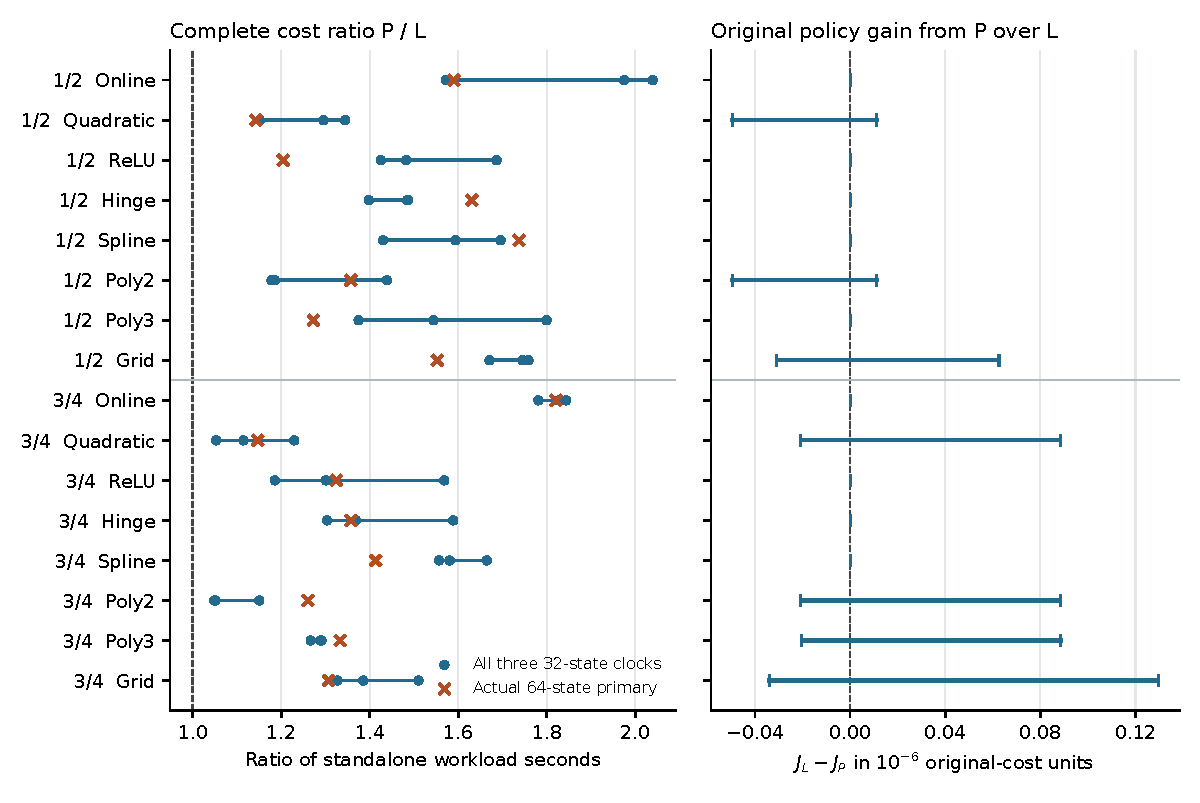
\includegraphics[width=\textwidth]{figures120/paired_legacy120.pdf}
\caption{Paired comparison versus inherited safe improvement in all sixteen
representation--risk cells. The left panel displays the complete-cost ratio
P/L from the primary 64-state cohort and each of the three matched 32-state
process clocks. Its range connects observed clocks and is not a confidence
interval. The right panel displays the independently reconstructed sample
mean original-policy contrast $J_L-J_P$ in $10^{-6}$ original-cost units;
positive values favor P. These are numerical enclosures on the common sample,
not population confidence intervals. Every cell is included; nine contrasts
are exact zero and the other seven contain zero. Exact rational values,
all clocks, plotting code and figure hashes are retained with the source.}
\label{fig:pairedlegacy120}
\end{figure}


\section{Conclusion}\label{sec:conclusion120}
Neural Bellman Operators connect learned continuation operators to feasible
decisions and the economic value of their implemented future behavior. The
construction requires a fixed original recursion and a complete accounting of
the information used by its critic, actor and numerical certificate. The
constrained investment model makes these requirements explicit while retaining
continuous innovations and nonlinear recursive risk.

The new action-comparison theory uses the geometry of the original Bellman
problem. A constrained state-gradient modulus yields an action-scaled
continuation-difference bound; convex integration and a constrained risk-defect
transfer then provide computable comparison intervals. Qualification and a
strict original-policy improvement bound jointly govern replacement of a
completed incumbent. The proof also identifies what additional precision can
resolve and what remains hidden behind a uniform future-policy allowance. This
distinction gives a concrete stopping criterion and a specified information
problem for subsequent NBO algorithms.

The independent experiment certifies gains over the completed learned
incumbents under the original investment objective. All 42 learned-incumbent
refinement groups have positive simultaneous population mean-gain lower bounds;
the independent optimum supports also give much smaller upper bounds on
original policy regret and root-mean-square optimal-action error. These gains coexist with a
strong online incumbent that is already close to optimal. The new paired
service changes twelve returned actions relative to inherited safe improvement,
but no cell-level incremental mean advantage is resolved, and all sixteen
primary costs and all forty-eight matched clocks are higher. The mixed
comparison authorizes one shared candidate at a recorded resolution where
the separate convex bound is inconclusive. The direct conventional proposal
has a strictly lower independently enclosed sample mean cost than both L and P
in five cells and is faster than P throughout the matched clocks. ReLU and
hinge policies are identical. ReLU has empty sufficient full-menu adoption
regions, and its upper-condition intersections across the three timing
scenarios are empty; individual-clock upper conditions leave some cases
unresolved. These findings preserve the independent neural contribution as an
explicit scientific problem.

The remaining research priorities concern the joint design of continuation
learning and paid economic decisions. They include acquisition losses that
reduce action-comparison work, information about the actual future controller
that resolves gains below the present allowance, and matched experiments with
longer horizons, multiple controls and higher-dimensional continuous risk.
The retained stochastic-control, recursive-utility and stopped-boundary results
provide separate rigorous foundations for this program. Progress on these
problems must preserve the original objective, give conventional methods the
same usable information, and demonstrate the economic value of the resulting
policies together with their full computational cost.


\section{Retained R120 author custody account}\label{dev:custody120}
This is the development companion of the R120 author revision. Its current
complete author baseline is R119, manuscript source
\nolinkurl{6250abfd317f3b2a56cb1303eb5ce78249bf4042}, with final publication
\nolinkurl{82618f037540233dda7d1ba8bfd3ddfdc88afbf9}. The controlling persisted
advisory remains R97 at
\nolinkurl{9723c6cd2cc8b3e071422f3e522d4a843946db63}, which assessed
\nolinkurl{f802fe64d91d9f5c1c8f86123b0fbe114e622279}. It is an owner-commissioned
advisory, rather than an Econometric Society editorial decision.

The prospective R120 scientific source is
\nolinkurl{369d02724cf12ae0e54390b4e7b5f894f703892e}. Its immutable protocol
and mathematical snapshot precede new acquisition, sampling and decisions.
All historical occurrences of ``current'' and ``new'' below refer to the
revision that originally wrote that material. Historical models, theorems,
proofs, numerical records, failures and negative results retain their own
source identity. R98 and R115 retain their independent preregistered constraints.
The current source, experiment, independent audit and PDF identities are
separately recorded in the referee-ready package.

\section{Complete R120 numerical reporting}\label{sec:developmentresults120}

This appendix displays the fixed all-arm census and retains every adverse or unresolved entry. Exact fraction endpoints and all raw counter dimensions accompany these rounded tables in tables120. C/L/P/D denote completed, legacy-safe, paired and direct-refine. Action error columns are independently justified upper bounds, never an observed distance to an exact optimizer. The original future controller, model, information access and accuracy requirement are unchanged.

\begingroup
\scriptsize
\setlength{\tabcolsep}{3pt}
\begin{longtable}{lllrrrrrr}
\caption{All 64 original objective and regret groups. Regret columns use $10^{-6}$ units; RMS is an optimal-action-error upper bound. Risk index 0/1 means $\alpha=1/2,3/4$.}\label{tab:allobjective120}\\
\toprule
Risk & Arm & Svc & Mean $J$ & Mean regret & Max regret & RMS bound & Changes & Steps \\ \midrule
\endfirsthead
\toprule
Risk & Arm & Svc & Mean $J$ & Mean regret & Max regret & RMS bound & Changes & Steps \\ \midrule
\endhead
\midrule\multicolumn{9}{r}{Continued on next page}\\\endfoot
\bottomrule\endlastfoot
0 & Online & C & [0.642910, 0.642911] & [0.000, 1.898] & 3.489 & 0.001378 & 0 & 0 \\
0 & Online & L & [0.642910, 0.642911] & [0.000, 1.898] & 3.489 & 0.001378 & 0 & 0 \\
0 & Online & P & [0.642910, 0.642911] & [0.000, 1.898] & 3.489 & 0.001378 & 0 & 0 \\
0 & Online & D & [0.642910, 0.642911] & [0.000, 1.898] & 3.489 & 0.001378 & 0 & 0 \\
0 & Quadratic & C & [0.643090, 0.643092] & [179.779, 182.168] & 856.586 & 0.013497 & 0 & 0 \\
0 & Quadratic & L & [0.642910, 0.642912] & [0.145, 2.387] & 4.406 & 0.001545 & 33 & 75 \\
0 & Quadratic & P & [0.642910, 0.642912] & [0.156, 2.405] & 4.406 & 0.001551 & 33 & 74 \\
0 & Quadratic & D & [0.642910, 0.642911] & [0.000, 1.906] & 3.489 & 0.001381 & 33 & 33 \\
0 & ReLU & C & [0.643124, 0.643125] & [213.694, 215.906] & 1945.935 & 0.014694 & 0 & 0 \\
0 & ReLU & L & [0.642910, 0.642912] & [0.473, 2.626] & 14.912 & 0.001620 & 21 & 49 \\
0 & ReLU & P & [0.642910, 0.642912] & [0.473, 2.626] & 14.912 & 0.001620 & 21 & 49 \\
0 & ReLU & D & [0.642910, 0.642911] & [0.000, 1.900] & 3.489 & 0.001378 & 21 & 21 \\
0 & Hinge & C & [0.643124, 0.643125] & [213.694, 215.906] & 1945.935 & 0.014694 & 0 & 0 \\
0 & Hinge & L & [0.642910, 0.642912] & [0.473, 2.626] & 14.912 & 0.001620 & 21 & 49 \\
0 & Hinge & P & [0.642910, 0.642912] & [0.473, 2.626] & 14.912 & 0.001620 & 21 & 49 \\
0 & Hinge & D & [0.642910, 0.642911] & [0.000, 1.900] & 3.489 & 0.001378 & 21 & 21 \\
0 & Spline & C & [0.643251, 0.643253] & [340.928, 343.135] & 2725.461 & 0.018524 & 0 & 0 \\
0 & Spline & L & [0.642910, 0.642912] & [0.167, 2.193] & 10.806 & 0.001481 & 22 & 36 \\
0 & Spline & P & [0.642910, 0.642912] & [0.167, 2.193] & 10.806 & 0.001481 & 22 & 36 \\
0 & Spline & D & [0.642910, 0.642911] & [0.000, 1.897] & 3.489 & 0.001377 & 22 & 22 \\
0 & Poly2 & C & [0.643090, 0.643092] & [179.784, 182.173] & 856.705 & 0.013497 & 0 & 0 \\
0 & Poly2 & L & [0.642910, 0.642912] & [0.145, 2.387] & 4.406 & 0.001545 & 33 & 75 \\
0 & Poly2 & P & [0.642910, 0.642912] & [0.156, 2.405] & 4.406 & 0.001551 & 33 & 74 \\
0 & Poly2 & D & [0.642910, 0.642911] & [0.000, 1.906] & 3.489 & 0.001381 & 33 & 33 \\
0 & Poly3 & C & [0.643145, 0.643147] & [234.872, 237.281] & 879.332 & 0.015404 & 0 & 0 \\
0 & Poly3 & L & [0.642910, 0.642912] & [0.501, 2.718] & 6.320 & 0.001649 & 33 & 71 \\
0 & Poly3 & P & [0.642910, 0.642912] & [0.501, 2.718] & 6.320 & 0.001649 & 33 & 71 \\
0 & Poly3 & D & [0.642910, 0.642911] & [0.000, 1.910] & 3.489 & 0.001382 & 33 & 33 \\
0 & Grid & C & [0.642928, 0.642930] & [18.405, 20.788] & 145.909 & 0.004559 & 0 & 0 \\
0 & Grid & L & [0.642910, 0.642912] & [0.021, 2.114] & 4.055 & 0.001454 & 30 & 48 \\
0 & Grid & P & [0.642910, 0.642912] & [0.021, 2.096] & 3.489 & 0.001448 & 31 & 49 \\
0 & Grid & D & [0.642910, 0.642911] & [0.003, 1.918] & 3.489 & 0.001385 & 31 & 31 \\
1 & Online & C & [0.654084, 0.654086] & [0.000, 1.850] & 7.307 & 0.001360 & 0 & 0 \\
1 & Online & L & [0.654084, 0.654086] & [0.000, 1.850] & 7.307 & 0.001360 & 0 & 0 \\
1 & Online & P & [0.654084, 0.654086] & [0.000, 1.850] & 7.307 & 0.001360 & 0 & 0 \\
1 & Online & D & [0.654084, 0.654086] & [0.000, 1.850] & 7.307 & 0.001360 & 0 & 0 \\
1 & Quadratic & C & [0.654278, 0.654280] & [193.829, 196.138] & 1032.104 & 0.014005 & 0 & 0 \\
1 & Quadratic & L & [0.654084, 0.654086] & [0.180, 2.375] & 7.307 & 0.001541 & 33 & 75 \\
1 & Quadratic & P & [0.654084, 0.654086] & [0.161, 2.341] & 7.307 & 0.001530 & 34 & 77 \\
1 & Quadratic & D & [0.654084, 0.654086] & [0.000, 1.851] & 7.307 & 0.001361 & 34 & 34 \\
1 & ReLU & C & [0.654247, 0.654249] & [163.246, 165.361] & 1921.805 & 0.012859 & 0 & 0 \\
1 & ReLU & L & [0.654085, 0.654086] & [0.353, 2.405] & 7.435 & 0.001551 & 20 & 45 \\
1 & ReLU & P & [0.654085, 0.654086] & [0.353, 2.405] & 7.435 & 0.001551 & 20 & 45 \\
1 & ReLU & D & [0.654084, 0.654086] & [0.000, 1.850] & 7.307 & 0.001360 & 20 & 20 \\
1 & Hinge & C & [0.654247, 0.654249] & [163.246, 165.361] & 1921.805 & 0.012859 & 0 & 0 \\
1 & Hinge & L & [0.654085, 0.654086] & [0.353, 2.405] & 7.435 & 0.001551 & 20 & 45 \\
1 & Hinge & P & [0.654085, 0.654086] & [0.353, 2.405] & 7.435 & 0.001551 & 20 & 45 \\
1 & Hinge & D & [0.654084, 0.654086] & [0.000, 1.850] & 7.307 & 0.001360 & 20 & 20 \\
1 & Spline & C & [0.654477, 0.654479] & [392.464, 394.637] & 2601.923 & 0.019865 & 0 & 0 \\
1 & Spline & L & [0.654084, 0.654086] & [0.381, 2.362] & 14.624 & 0.001537 & 24 & 39 \\
1 & Spline & P & [0.654084, 0.654086] & [0.381, 2.362] & 14.624 & 0.001537 & 24 & 39 \\
1 & Spline & D & [0.654084, 0.654086] & [0.000, 1.850] & 7.307 & 0.001360 & 24 & 24 \\
1 & Poly2 & C & [0.654278, 0.654280] & [193.829, 196.137] & 1032.104 & 0.014005 & 0 & 0 \\
1 & Poly2 & L & [0.654084, 0.654086] & [0.180, 2.375] & 7.307 & 0.001541 & 33 & 75 \\
1 & Poly2 & P & [0.654084, 0.654086] & [0.161, 2.341] & 7.307 & 0.001530 & 34 & 77 \\
1 & Poly2 & D & [0.654084, 0.654086] & [0.000, 1.851] & 7.307 & 0.001361 & 34 & 34 \\
1 & Poly3 & C & [0.654314, 0.654316] & [230.003, 232.293] & 893.109 & 0.015241 & 0 & 0 \\
1 & Poly3 & L & [0.654085, 0.654087] & [0.522, 2.676] & 7.307 & 0.001636 & 32 & 70 \\
1 & Poly3 & P & [0.654085, 0.654087] & [0.499, 2.642] & 7.307 & 0.001625 & 32 & 72 \\
1 & Poly3 & D & [0.654084, 0.654086] & [0.000, 1.860] & 7.307 & 0.001364 & 32 & 32 \\
1 & Grid & C & [0.654127, 0.654129] & [42.944, 45.242] & 356.447 & 0.006726 & 0 & 0 \\
1 & Grid & L & [0.654084, 0.654086] & [0.058, 2.144] & 7.307 & 0.001464 & 33 & 55 \\
1 & Grid & P & [0.654084, 0.654086] & [0.034, 2.096] & 7.307 & 0.001448 & 33 & 58 \\
1 & Grid & D & [0.654084, 0.654086] & [0.000, 1.856] & 7.307 & 0.001362 & 33 & 33 \\
\end{longtable}
\endgroup


\begingroup
\scriptsize
\setlength{\tabcolsep}{3pt}
\begin{longtable}{lllrrrrrrr}
\caption{All 64 cost decompositions in seconds. A is the complete standalone acquisition charge; T64 includes load, service and logging. The last column retains the median and full range of all three T32 clocks. Event-serialization clocks overlap service time and are not added twice.}\label{tab:allcost120}\\
\toprule
Risk & Arm & Svc & A & T64 & Service & Load & Records & Other & T32: med [range] \\ \midrule
\endfirsthead
\toprule
Risk & Arm & Svc & A & T64 & Service & Load & Records & Other & T32: med [range] \\ \midrule
\endhead
\midrule\multicolumn{10}{r}{Continued on next page}\\\endfoot
\bottomrule\endlastfoot
0 & Online & C & 0.001 & 1.886 & 1.803 & 0.000027 & 0.044 & 0.040 & 0.885 [0.828, 0.936] \\
0 & Online & L & 0.001 & 7.341 & 7.137 & 0.000045 & 0.155 & 0.048 & 2.742 [2.695, 3.699] \\
0 & Online & P & 0.001 & 11.673 & 11.280 & 0.000067 & 0.340 & 0.052 & 5.594 [5.325, 5.816] \\
0 & Online & D & 0.001 & 6.838 & 6.454 & 0.000037 & 0.301 & 0.083 & 3.167 [2.967, 3.437] \\
0 & Quadratic & C & 0.085 & 2.059 & 1.554 & 0.000076 & 0.075 & 0.430 & 0.613 [0.590, 0.658] \\
0 & Quadratic & L & 0.085 & 6.234 & 5.760 & 0.000064 & 0.390 & 0.083 & 2.716 [2.410, 2.962] \\
0 & Quadratic & P & 0.085 & 7.135 & 6.817 & 0.000083 & 0.264 & 0.053 & 3.424 [3.268, 3.543] \\
0 & Quadratic & D & 0.085 & 4.356 & 4.214 & 0.000085 & 0.098 & 0.044 & 2.334 [1.985, 2.447] \\
0 & ReLU & C & 0.081 & 1.655 & 1.549 & 0.000056 & 0.054 & 0.052 & 0.806 [0.799, 0.828] \\
0 & ReLU & L & 0.081 & 7.301 & 6.944 & 0.000103 & 0.274 & 0.082 & 2.846 [2.793, 2.928] \\
0 & ReLU & P & 0.081 & 8.810 & 8.443 & 0.000116 & 0.314 & 0.052 & 4.180 [4.090, 4.995] \\
0 & ReLU & D & 0.081 & 5.475 & 5.299 & 0.000159 & 0.129 & 0.046 & 2.749 [2.452, 2.774] \\
0 & Hinge & C & 0.081 & 1.655 & 1.570 & 0.000039 & 0.046 & 0.039 & 0.834 [0.712, 0.843] \\
0 & Hinge & L & 0.081 & 5.656 & 5.484 & 0.000049 & 0.128 & 0.044 & 2.808 [2.772, 2.908] \\
0 & Hinge & P & 0.081 & 9.276 & 8.897 & 0.000073 & 0.328 & 0.050 & 4.161 [4.096, 4.209] \\
0 & Hinge & D & 0.081 & 5.510 & 5.317 & 0.000066 & 0.144 & 0.048 & 2.499 [2.439, 2.686] \\
0 & Spline & C & 0.081 & 1.653 & 1.570 & 0.000096 & 0.044 & 0.039 & 0.952 [0.818, 1.203] \\
0 & Spline & L & 0.081 & 5.677 & 5.490 & 0.000058 & 0.144 & 0.043 & 3.361 [2.756, 3.661] \\
0 & Spline & P & 0.081 & 9.923 & 9.578 & 0.000072 & 0.297 & 0.048 & 4.842 [4.730, 5.883] \\
0 & Spline & D & 0.081 & 5.432 & 5.255 & 0.000141 & 0.132 & 0.046 & 3.333 [2.727, 3.857] \\
0 & Poly2 & C & 0.012 & 1.302 & 1.218 & 0.000036 & 0.044 & 0.039 & 0.630 [0.578, 0.751] \\
0 & Poly2 & L & 0.012 & 5.065 & 4.909 & 0.000044 & 0.116 & 0.039 & 3.100 [2.466, 3.260] \\
0 & Poly2 & P & 0.012 & 6.878 & 6.602 & 0.000045 & 0.228 & 0.047 & 3.653 [3.553, 3.867] \\
0 & Poly2 & D & 0.012 & 4.242 & 4.096 & 0.000055 & 0.100 & 0.046 & 2.167 [2.081, 2.213] \\
0 & Poly3 & C & 0.011 & 1.289 & 1.207 & 0.000039 & 0.045 & 0.037 & 0.752 [0.649, 0.768] \\
0 & Poly3 & L & 0.011 & 5.632 & 5.454 & 0.000052 & 0.131 & 0.046 & 3.042 [2.444, 3.126] \\
0 & Poly3 & P & 0.011 & 7.171 & 6.804 & 0.000051 & 0.315 & 0.051 & 4.407 [4.302, 4.703] \\
0 & Poly3 & D & 0.011 & 4.654 & 4.490 & 0.000051 & 0.115 & 0.048 & 2.127 [2.011, 2.401] \\
0 & Grid & C & 0.011 & 1.429 & 1.346 & 0.000201 & 0.043 & 0.039 & 0.704 [0.590, 0.786] \\
0 & Grid & L & 0.011 & 5.788 & 5.568 & 0.000118 & 0.167 & 0.053 & 2.575 [2.502, 2.584] \\
0 & Grid & P & 0.011 & 8.993 & 8.587 & 0.000129 & 0.354 & 0.053 & 4.373 [4.308, 4.553] \\
0 & Grid & D & 0.011 & 4.528 & 4.375 & 0.000154 & 0.109 & 0.044 & 2.395 [2.351, 2.532] \\
1 & Online & C & 0.002 & 1.895 & 1.805 & 0.000211 & 0.049 & 0.041 & 0.899 [0.804, 1.136] \\
1 & Online & L & 0.002 & 5.821 & 5.649 & 0.000038 & 0.131 & 0.041 & 2.999 [2.940, 3.126] \\
1 & Online & P & 0.002 & 10.600 & 10.213 & 0.000037 & 0.342 & 0.046 & 5.480 [5.237, 5.766] \\
1 & Online & D & 0.002 & 6.430 & 6.231 & 0.000041 & 0.151 & 0.047 & 3.208 [3.087, 3.243] \\
1 & Quadratic & C & 0.081 & 1.405 & 1.309 & 0.000397 & 0.050 & 0.046 & 0.526 [0.522, 0.587] \\
1 & Quadratic & L & 0.081 & 5.100 & 4.876 & 0.000121 & 0.172 & 0.052 & 2.542 [2.379, 2.752] \\
1 & Quadratic & P & 0.081 & 5.860 & 5.606 & 0.000080 & 0.210 & 0.044 & 2.944 [2.681, 3.077] \\
1 & Quadratic & D & 0.081 & 3.473 & 3.358 & 0.000072 & 0.078 & 0.037 & 1.870 [1.805, 1.993] \\
1 & ReLU & C & 0.069 & 1.757 & 1.677 & 0.000263 & 0.042 & 0.037 & 0.850 [0.791, 0.873] \\
1 & ReLU & L & 0.069 & 5.745 & 5.568 & 0.000066 & 0.133 & 0.044 & 3.279 [2.645, 3.476] \\
1 & ReLU & P & 0.069 & 7.632 & 7.342 & 0.000077 & 0.246 & 0.044 & 4.188 [4.133, 4.286] \\
1 & ReLU & D & 0.069 & 5.357 & 5.187 & 0.000076 & 0.125 & 0.045 & 2.502 [2.499, 2.585] \\
1 & Hinge & C & 0.067 & 2.120 & 2.017 & 0.000232 & 0.051 & 0.052 & 0.878 [0.781, 0.903] \\
1 & Hinge & L & 0.067 & 6.585 & 6.383 & 0.000087 & 0.154 & 0.048 & 3.009 [2.985, 3.083] \\
1 & Hinge & P & 0.067 & 8.964 & 8.625 & 0.000052 & 0.290 & 0.049 & 4.245 [3.943, 4.781] \\
1 & Hinge & D & 0.067 & 5.897 & 5.712 & 0.000053 & 0.135 & 0.050 & 2.658 [2.310, 2.994] \\
1 & Spline & C & 0.050 & 1.990 & 1.871 & 0.000279 & 0.064 & 0.055 & 0.808 [0.774, 0.820] \\
1 & Spline & L & 0.050 & 6.165 & 5.956 & 0.000066 & 0.154 & 0.054 & 2.978 [2.701, 3.111] \\
1 & Spline & P & 0.050 & 8.732 & 8.411 & 0.000070 & 0.279 & 0.043 & 4.737 [4.530, 4.871] \\
1 & Spline & D & 0.050 & 5.532 & 5.344 & 0.000078 & 0.138 & 0.050 & 2.634 [2.494, 2.738] \\
1 & Poly2 & C & 0.010 & 1.374 & 1.266 & 0.000355 & 0.063 & 0.045 & 0.695 [0.681, 0.772] \\
1 & Poly2 & L & 0.010 & 5.263 & 5.097 & 0.000046 & 0.124 & 0.042 & 3.038 [2.902, 3.122] \\
1 & Poly2 & P & 0.010 & 6.635 & 6.346 & 0.000054 & 0.244 & 0.045 & 3.185 [3.051, 3.593] \\
1 & Poly2 & D & 0.010 & 3.729 & 3.607 & 0.000045 & 0.082 & 0.040 & 2.048 [2.027, 2.061] \\
1 & Poly3 & C & 0.010 & 1.321 & 1.243 & 0.000235 & 0.040 & 0.037 & 0.774 [0.772, 0.877] \\
1 & Poly3 & L & 0.010 & 5.106 & 4.941 & 0.000111 & 0.124 & 0.041 & 2.810 [2.564, 2.883] \\
1 & Poly3 & P & 0.010 & 6.809 & 6.544 & 0.000050 & 0.219 & 0.047 & 3.623 [3.313, 3.655] \\
1 & Poly3 & D & 0.010 & 4.002 & 3.877 & 0.000049 & 0.083 & 0.043 & 2.130 [2.090, 2.369] \\
1 & Grid & C & 0.010 & 1.240 & 1.156 & 0.000259 & 0.044 & 0.040 & 0.679 [0.656, 0.861] \\
1 & Grid & L & 0.010 & 5.335 & 5.175 & 0.000139 & 0.119 & 0.041 & 3.061 [2.929, 3.103] \\
1 & Grid & P & 0.010 & 6.975 & 6.683 & 0.000108 & 0.248 & 0.044 & 4.302 [3.890, 4.628] \\
1 & Grid & D & 0.010 & 4.186 & 4.052 & 0.000152 & 0.092 & 0.042 & 2.201 [2.144, 2.592] \\
\end{longtable}
\endgroup


\begingroup
\scriptsize
\setlength{\tabcolsep}{3pt}
\begin{longtable}{lllrrrrrrrr}
\caption{All candidate and certificate outcomes. Candidates and precision levels count different units. Refused candidates and exhausted ladders remain paid in every measured service.}\label{tab:alltrials120}\\
\toprule
Risk & Arm & Svc & Candidates & Levels & Unqual. & Nonimpr. & Exhaust & Equal & First rej. & Fallback \\ \midrule
\endfirsthead
\toprule
Risk & Arm & Svc & Candidates & Levels & Unqual. & Nonimpr. & Exhaust & Equal & First rej. & Fallback \\ \midrule
\endhead
\midrule\multicolumn{11}{r}{Continued on next page}\\\endfoot
\bottomrule\endlastfoot
0 & Online & C & 0 & 0 & 0 & 0 & 0 & 0 & 0 & 0 \\
0 & Online & L & 192 & 0 & 0 & 0 & 0 & 0 & 0 & 0 \\
0 & Online & P & 192 & 630 & 102 & 0 & 105 & 87 & 0 & 0 \\
0 & Online & D & 64 & 210 & 34 & 0 & 35 & 29 & 0 & 0 \\
0 & Quadratic & C & 0 & 0 & 0 & 0 & 0 & 0 & 0 & 0 \\
0 & Quadratic & L & 192 & 0 & 0 & 0 & 0 & 0 & 0 & 0 \\
0 & Quadratic & P & 192 & 381 & 102 & 12 & 19 & 87 & 0 & 0 \\
0 & Quadratic & D & 64 & 94 & 34 & 0 & 2 & 29 & 0 & 0 \\
0 & ReLU & C & 0 & 0 & 0 & 0 & 0 & 0 & 17 & 0 \\
0 & ReLU & L & 192 & 0 & 1 & 0 & 0 & 0 & 17 & 0 \\
0 & ReLU & P & 192 & 478 & 103 & 3 & 55 & 85 & 17 & 0 \\
0 & ReLU & D & 64 & 141 & 36 & 0 & 16 & 27 & 17 & 0 \\
0 & Hinge & C & 0 & 0 & 0 & 0 & 0 & 0 & 17 & 0 \\
0 & Hinge & L & 192 & 0 & 1 & 0 & 0 & 0 & 17 & 0 \\
0 & Hinge & P & 192 & 478 & 103 & 3 & 55 & 85 & 17 & 0 \\
0 & Hinge & D & 64 & 141 & 36 & 0 & 16 & 27 & 17 & 0 \\
0 & Spline & C & 0 & 0 & 0 & 0 & 0 & 0 & 21 & 0 \\
0 & Spline & L & 192 & 0 & 0 & 0 & 0 & 0 & 21 & 0 \\
0 & Spline & P & 192 & 544 & 110 & 5 & 72 & 79 & 21 & 0 \\
0 & Spline & D & 64 & 174 & 42 & 0 & 21 & 21 & 21 & 0 \\
0 & Poly2 & C & 0 & 0 & 0 & 0 & 0 & 0 & 0 & 0 \\
0 & Poly2 & L & 192 & 0 & 0 & 0 & 0 & 0 & 0 & 0 \\
0 & Poly2 & P & 192 & 381 & 102 & 12 & 19 & 87 & 0 & 0 \\
0 & Poly2 & D & 64 & 94 & 34 & 0 & 2 & 29 & 0 & 0 \\
0 & Poly3 & C & 0 & 0 & 0 & 0 & 0 & 0 & 0 & 0 \\
0 & Poly3 & L & 192 & 0 & 0 & 0 & 0 & 0 & 0 & 0 \\
0 & Poly3 & P & 192 & 384 & 104 & 8 & 27 & 86 & 0 & 0 \\
0 & Poly3 & D & 64 & 89 & 35 & 0 & 3 & 28 & 0 & 0 \\
0 & Grid & C & 0 & 0 & 0 & 0 & 0 & 0 & 0 & 0 \\
0 & Grid & L & 192 & 0 & 0 & 0 & 0 & 0 & 0 & 0 \\
0 & Grid & P & 192 & 515 & 102 & 6 & 50 & 87 & 0 & 0 \\
0 & Grid & D & 64 & 134 & 34 & 0 & 4 & 29 & 0 & 0 \\
1 & Online & C & 0 & 0 & 0 & 0 & 0 & 0 & 0 & 0 \\
1 & Online & L & 192 & 0 & 0 & 0 & 0 & 0 & 0 & 0 \\
1 & Online & P & 192 & 630 & 0 & 0 & 105 & 87 & 0 & 0 \\
1 & Online & D & 64 & 210 & 0 & 0 & 35 & 29 & 0 & 0 \\
1 & Quadratic & C & 0 & 0 & 0 & 0 & 0 & 0 & 0 & 0 \\
1 & Quadratic & L & 192 & 0 & 0 & 0 & 0 & 0 & 0 & 0 \\
1 & Quadratic & P & 192 & 301 & 0 & 12 & 16 & 87 & 0 & 0 \\
1 & Quadratic & D & 64 & 58 & 0 & 0 & 1 & 29 & 0 & 0 \\
1 & ReLU & C & 0 & 0 & 0 & 0 & 0 & 0 & 20 & 0 \\
1 & ReLU & L & 192 & 0 & 1 & 0 & 0 & 0 & 20 & 0 \\
1 & ReLU & P & 192 & 442 & 1 & 3 & 59 & 85 & 20 & 0 \\
1 & ReLU & D & 64 & 125 & 0 & 0 & 17 & 27 & 20 & 0 \\
1 & Hinge & C & 0 & 0 & 0 & 0 & 0 & 0 & 20 & 0 \\
1 & Hinge & L & 192 & 0 & 1 & 0 & 0 & 0 & 20 & 0 \\
1 & Hinge & P & 192 & 442 & 1 & 3 & 59 & 85 & 20 & 0 \\
1 & Hinge & D & 64 & 125 & 0 & 0 & 17 & 27 & 20 & 0 \\
1 & Spline & C & 0 & 0 & 0 & 0 & 0 & 0 & 19 & 0 \\
1 & Spline & L & 192 & 0 & 0 & 0 & 0 & 0 & 19 & 0 \\
1 & Spline & P & 192 & 485 & 0 & 7 & 67 & 79 & 19 & 0 \\
1 & Spline & D & 64 & 146 & 0 & 0 & 19 & 21 & 19 & 0 \\
1 & Poly2 & C & 0 & 0 & 0 & 0 & 0 & 0 & 0 & 0 \\
1 & Poly2 & L & 192 & 0 & 0 & 0 & 0 & 0 & 0 & 0 \\
1 & Poly2 & P & 192 & 301 & 0 & 12 & 16 & 87 & 0 & 0 \\
1 & Poly2 & D & 64 & 58 & 0 & 0 & 1 & 29 & 0 & 0 \\
1 & Poly3 & C & 0 & 0 & 0 & 0 & 0 & 0 & 0 & 0 \\
1 & Poly3 & L & 192 & 0 & 0 & 0 & 0 & 0 & 0 & 0 \\
1 & Poly3 & P & 192 & 295 & 0 & 9 & 24 & 87 & 0 & 0 \\
1 & Poly3 & D & 64 & 56 & 0 & 0 & 3 & 29 & 0 & 0 \\
1 & Grid & C & 0 & 0 & 0 & 0 & 0 & 0 & 0 & 0 \\
1 & Grid & L & 192 & 0 & 0 & 0 & 0 & 0 & 0 & 0 \\
1 & Grid & P & 192 & 397 & 0 & 10 & 37 & 87 & 0 & 0 \\
1 & Grid & D & 64 & 77 & 0 & 0 & 2 & 29 & 0 & 0 \\
\end{longtable}
\endgroup


\begingroup
\scriptsize
\setlength{\tabcolsep}{3pt}
\begin{longtable}{lllrrrrrrr}
\caption{All recorded paired-bound activity. Need-upper identifies accepted levels whose separate convex-only scalar upper is nonnegative. Need-transfer identifies certified rejections whose lower remains negative with the directly measured incumbent slack. Neither is a counterfactual timing experiment.}\label{tab:allpairuse120}\\
\toprule
Risk & Arm & Svc & Densities & Levels & Paid rows & Sqrts & Upper active & Need upper & Need transfer \\ \midrule
\endfirsthead
\toprule
Risk & Arm & Svc & Densities & Levels & Paid rows & Sqrts & Upper active & Need upper & Need transfer \\ \midrule
\endhead
\midrule\multicolumn{10}{r}{Continued on next page}\\\endfoot
\bottomrule\endlastfoot
0 & Online & C & 0 & 0 & 0 & 0 & 0 & 0 & 0 \\
0 & Online & L & 0 & 0 & 0 & 0 & 0 & 0 & 0 \\
0 & Online & P & 105 & 630 & 58824 & 210 & 630 & 0 & 0 \\
0 & Online & D & 35 & 210 & 19608 & 70 & 210 & 0 & 0 \\
0 & Quadratic & C & 0 & 0 & 0 & 0 & 0 & 0 & 0 \\
0 & Quadratic & L & 0 & 0 & 0 & 0 & 0 & 0 & 0 \\
0 & Quadratic & P & 105 & 381 & 20584 & 210 & 167 & 0 & 0 \\
0 & Quadratic & D & 35 & 94 & 2870 & 70 & 16 & 0 & 0 \\
0 & ReLU & C & 0 & 0 & 0 & 0 & 0 & 0 & 0 \\
0 & ReLU & L & 0 & 0 & 0 & 0 & 0 & 0 & 0 \\
0 & ReLU & P & 107 & 478 & 35856 & 214 & 352 & 0 & 0 \\
0 & ReLU & D & 37 & 141 & 10006 & 74 & 98 & 0 & 0 \\
0 & Hinge & C & 0 & 0 & 0 & 0 & 0 & 0 & 0 \\
0 & Hinge & L & 0 & 0 & 0 & 0 & 0 & 0 & 0 \\
0 & Hinge & P & 107 & 478 & 35856 & 214 & 352 & 0 & 0 \\
0 & Hinge & D & 37 & 141 & 10006 & 74 & 98 & 0 & 0 \\
0 & Spline & C & 0 & 0 & 0 & 0 & 0 & 0 & 0 \\
0 & Spline & L & 0 & 0 & 0 & 0 & 0 & 0 & 0 \\
0 & Spline & P & 113 & 544 & 43526 & 226 & 437 & 0 & 0 \\
0 & Spline & D & 43 & 174 & 12776 & 86 & 128 & 0 & 0 \\
0 & Poly2 & C & 0 & 0 & 0 & 0 & 0 & 0 & 0 \\
0 & Poly2 & L & 0 & 0 & 0 & 0 & 0 & 0 & 0 \\
0 & Poly2 & P & 105 & 381 & 20584 & 210 & 167 & 0 & 0 \\
0 & Poly2 & D & 35 & 94 & 2870 & 70 & 16 & 0 & 0 \\
0 & Poly3 & C & 0 & 0 & 0 & 0 & 0 & 0 & 0 \\
0 & Poly3 & L & 0 & 0 & 0 & 0 & 0 & 0 & 0 \\
0 & Poly3 & P & 106 & 384 & 22734 & 212 & 158 & 1 & 0 \\
0 & Poly3 & D & 36 & 89 & 2788 & 72 & 19 & 1 & 0 \\
0 & Grid & C & 0 & 0 & 0 & 0 & 0 & 0 & 0 \\
0 & Grid & L & 0 & 0 & 0 & 0 & 0 & 0 & 0 \\
0 & Grid & P & 105 & 515 & 38676 & 210 & 267 & 0 & 0 \\
0 & Grid & D & 35 & 134 & 7158 & 70 & 47 & 0 & 0 \\
1 & Online & C & 0 & 0 & 0 & 0 & 0 & 0 & 0 \\
1 & Online & L & 0 & 0 & 0 & 0 & 0 & 0 & 0 \\
1 & Online & P & 105 & 630 & 54180 & 210 & 630 & 0 & 0 \\
1 & Online & D & 35 & 210 & 18060 & 70 & 210 & 0 & 0 \\
1 & Quadratic & C & 0 & 0 & 0 & 0 & 0 & 0 & 0 \\
1 & Quadratic & L & 0 & 0 & 0 & 0 & 0 & 0 & 0 \\
1 & Quadratic & P & 105 & 301 & 14418 & 210 & 111 & 0 & 0 \\
1 & Quadratic & D & 35 & 58 & 1452 & 70 & 7 & 0 & 0 \\
1 & ReLU & C & 0 & 0 & 0 & 0 & 0 & 0 & 0 \\
1 & ReLU & L & 0 & 0 & 0 & 0 & 0 & 0 & 0 \\
1 & ReLU & P & 107 & 442 & 32044 & 214 & 347 & 0 & 0 \\
1 & ReLU & D & 37 & 125 & 9026 & 74 & 102 & 0 & 0 \\
1 & Hinge & C & 0 & 0 & 0 & 0 & 0 & 0 & 0 \\
1 & Hinge & L & 0 & 0 & 0 & 0 & 0 & 0 & 0 \\
1 & Hinge & P & 107 & 442 & 32044 & 214 & 347 & 0 & 0 \\
1 & Hinge & D & 37 & 125 & 9026 & 74 & 102 & 0 & 0 \\
1 & Spline & C & 0 & 0 & 0 & 0 & 0 & 0 & 0 \\
1 & Spline & L & 0 & 0 & 0 & 0 & 0 & 0 & 0 \\
1 & Spline & P & 113 & 485 & 36226 & 226 & 392 & 0 & 0 \\
1 & Spline & D & 43 & 146 & 10380 & 86 & 116 & 0 & 0 \\
1 & Poly2 & C & 0 & 0 & 0 & 0 & 0 & 0 & 0 \\
1 & Poly2 & L & 0 & 0 & 0 & 0 & 0 & 0 & 0 \\
1 & Poly2 & P & 105 & 301 & 14418 & 210 & 111 & 0 & 0 \\
1 & Poly2 & D & 35 & 58 & 1452 & 70 & 7 & 0 & 0 \\
1 & Poly3 & C & 0 & 0 & 0 & 0 & 0 & 0 & 0 \\
1 & Poly3 & L & 0 & 0 & 0 & 0 & 0 & 0 & 0 \\
1 & Poly3 & P & 105 & 295 & 16102 & 210 & 123 & 0 & 0 \\
1 & Poly3 & D & 35 & 56 & 2008 & 70 & 12 & 0 & 0 \\
1 & Grid & C & 0 & 0 & 0 & 0 & 0 & 0 & 0 \\
1 & Grid & L & 0 & 0 & 0 & 0 & 0 & 0 & 0 \\
1 & Grid & P & 105 & 397 & 24514 & 210 & 168 & 0 & 0 \\
1 & Grid & D & 35 & 77 & 2450 & 70 & 14 & 0 & 0 \\
\end{longtable}
\endgroup


\begingroup
\scriptsize
\setlength{\tabcolsep}{3pt}
\begin{longtable}{lllrrrrrr}
\caption{All 192 raw 32-state cohort clocks and matched-repeat ratios. Timing repetitions are descriptive observations on the same first 32 states and are not new population units.}\label{tab:allclocks120}\\
\toprule
Risk & Arm & Svc & Rep & T32 & Service & Load & T32/C & Full/C \\ \midrule
\endfirsthead
\toprule
Risk & Arm & Svc & Rep & T32 & Service & Load & T32/C & Full/C \\ \midrule
\endhead
\midrule\multicolumn{9}{r}{Continued on next page}\\\endfoot
\bottomrule\endlastfoot
0 & Online & C & 0 & 0.885 & 0.844 & 0.000026 & 1.000 & 1.000 \\
0 & Online & L & 0 & 2.742 & 2.662 & 0.000064 & 3.099 & 3.097 \\
0 & Online & P & 0 & 5.594 & 5.374 & 0.000035 & 6.321 & 6.316 \\
0 & Online & D & 0 & 2.967 & 2.880 & 0.000037 & 3.353 & 3.351 \\
0 & Quadratic & C & 0 & 0.590 & 0.550 & 0.000063 & 1.000 & 1.000 \\
0 & Quadratic & L & 0 & 2.716 & 2.630 & 0.000058 & 4.602 & 4.147 \\
0 & Quadratic & P & 0 & 3.543 & 3.393 & 0.000067 & 6.004 & 5.372 \\
0 & Quadratic & D & 0 & 1.985 & 1.917 & 0.000066 & 3.364 & 3.066 \\
0 & ReLU & C & 0 & 0.799 & 0.753 & 0.000128 & 1.000 & 1.000 \\
0 & ReLU & L & 0 & 2.846 & 2.760 & 0.000061 & 3.561 & 3.325 \\
0 & ReLU & P & 0 & 4.090 & 3.946 & 0.000040 & 5.117 & 4.739 \\
0 & ReLU & D & 0 & 2.749 & 2.661 & 0.000067 & 3.439 & 3.215 \\
0 & Hinge & C & 0 & 0.843 & 0.796 & 0.000050 & 1.000 & 1.000 \\
0 & Hinge & L & 0 & 2.908 & 2.819 & 0.000068 & 3.448 & 3.233 \\
0 & Hinge & P & 0 & 4.096 & 3.942 & 0.000047 & 4.857 & 4.518 \\
0 & Hinge & D & 0 & 2.439 & 2.365 & 0.000039 & 2.892 & 2.726 \\
0 & Spline & C & 0 & 0.818 & 0.777 & 0.000059 & 1.000 & 1.000 \\
0 & Spline & L & 0 & 3.361 & 3.266 & 0.000074 & 4.108 & 3.827 \\
0 & Spline & P & 0 & 4.842 & 4.671 & 0.000214 & 5.917 & 5.474 \\
0 & Spline & D & 0 & 3.333 & 3.241 & 0.000067 & 4.074 & 3.797 \\
0 & Poly2 & C & 0 & 0.751 & 0.705 & 0.000042 & 1.000 & 1.000 \\
0 & Poly2 & L & 0 & 3.100 & 2.997 & 0.000222 & 4.126 & 4.076 \\
0 & Poly2 & P & 0 & 3.653 & 3.501 & 0.000062 & 4.863 & 4.800 \\
0 & Poly2 & D & 0 & 2.213 & 2.140 & 0.000046 & 2.946 & 2.914 \\
0 & Poly3 & C & 0 & 0.768 & 0.709 & 0.000077 & 1.000 & 1.000 \\
0 & Poly3 & L & 0 & 3.042 & 2.946 & 0.000061 & 3.962 & 3.919 \\
0 & Poly3 & P & 0 & 4.703 & 4.507 & 0.000231 & 6.127 & 6.052 \\
0 & Poly3 & D & 0 & 2.401 & 2.316 & 0.000222 & 3.128 & 3.097 \\
0 & Grid & C & 0 & 0.590 & 0.552 & 0.000118 & 1.000 & 1.000 \\
0 & Grid & L & 0 & 2.584 & 2.494 & 0.000115 & 4.383 & 4.323 \\
0 & Grid & P & 0 & 4.553 & 4.353 & 0.000130 & 7.723 & 7.603 \\
0 & Grid & D & 0 & 2.395 & 2.311 & 0.000297 & 4.062 & 4.008 \\
1 & Online & C & 0 & 0.804 & 0.767 & 0.000038 & 1.000 & 1.000 \\
1 & Online & L & 0 & 3.126 & 3.037 & 0.000233 & 3.890 & 3.884 \\
1 & Online & P & 0 & 5.766 & 5.553 & 0.000039 & 7.175 & 7.161 \\
1 & Online & D & 0 & 3.087 & 2.985 & 0.000042 & 3.842 & 3.836 \\
1 & Quadratic & C & 0 & 0.587 & 0.544 & 0.000072 & 1.000 & 1.000 \\
1 & Quadratic & L & 0 & 2.542 & 2.458 & 0.000065 & 4.329 & 3.928 \\
1 & Quadratic & P & 0 & 2.681 & 2.576 & 0.000196 & 4.565 & 4.135 \\
1 & Quadratic & D & 0 & 1.805 & 1.748 & 0.000061 & 3.073 & 2.823 \\
1 & ReLU & C & 0 & 0.873 & 0.830 & 0.000079 & 1.000 & 1.000 \\
1 & ReLU & L & 0 & 2.645 & 2.562 & 0.000058 & 3.031 & 2.882 \\
1 & ReLU & P & 0 & 4.188 & 4.025 & 0.000060 & 4.799 & 4.520 \\
1 & ReLU & D & 0 & 2.502 & 2.426 & 0.000276 & 2.867 & 2.730 \\
1 & Hinge & C & 0 & 0.878 & 0.832 & 0.000309 & 1.000 & 1.000 \\
1 & Hinge & L & 0 & 3.083 & 2.991 & 0.000053 & 3.511 & 3.332 \\
1 & Hinge & P & 0 & 4.245 & 4.090 & 0.000055 & 4.833 & 4.560 \\
1 & Hinge & D & 0 & 2.994 & 2.903 & 0.000050 & 3.409 & 3.237 \\
1 & Spline & C & 0 & 0.808 & 0.762 & 0.000082 & 1.000 & 1.000 \\
1 & Spline & L & 0 & 3.111 & 3.006 & 0.000282 & 3.848 & 3.682 \\
1 & Spline & P & 0 & 4.871 & 4.693 & 0.000091 & 6.025 & 5.732 \\
1 & Spline & D & 0 & 2.634 & 2.543 & 0.000066 & 3.258 & 3.127 \\
1 & Poly2 & C & 0 & 0.681 & 0.633 & 0.000054 & 1.000 & 1.000 \\
1 & Poly2 & L & 0 & 2.902 & 2.805 & 0.000048 & 4.264 & 4.216 \\
1 & Poly2 & P & 0 & 3.051 & 2.927 & 0.000187 & 4.482 & 4.431 \\
1 & Poly2 & D & 0 & 2.061 & 1.997 & 0.000051 & 3.028 & 2.999 \\
1 & Poly3 & C & 0 & 0.774 & 0.727 & 0.000052 & 1.000 & 1.000 \\
1 & Poly3 & L & 0 & 2.883 & 2.766 & 0.000048 & 3.726 & 3.690 \\
1 & Poly3 & P & 0 & 3.655 & 3.520 & 0.000043 & 4.723 & 4.674 \\
1 & Poly3 & D & 0 & 2.090 & 2.020 & 0.000197 & 2.702 & 2.679 \\
1 & Grid & C & 0 & 0.656 & 0.612 & 0.000283 & 1.000 & 1.000 \\
1 & Grid & L & 0 & 3.061 & 2.962 & 0.000163 & 4.665 & 4.611 \\
1 & Grid & P & 0 & 4.628 & 4.436 & 0.000122 & 7.053 & 6.964 \\
1 & Grid & D & 0 & 2.201 & 2.125 & 0.000138 & 3.354 & 3.319 \\
0 & Online & C & 1 & 0.828 & 0.786 & 0.000040 & 1.000 & 1.000 \\
0 & Online & L & 1 & 2.695 & 2.615 & 0.000028 & 3.257 & 3.255 \\
0 & Online & P & 1 & 5.325 & 5.137 & 0.000040 & 6.434 & 6.428 \\
0 & Online & D & 1 & 3.167 & 3.050 & 0.000041 & 3.827 & 3.824 \\
0 & Quadratic & C & 1 & 0.658 & 0.606 & 0.000063 & 1.000 & 1.000 \\
0 & Quadratic & L & 1 & 2.410 & 2.322 & 0.000060 & 3.660 & 3.355 \\
0 & Quadratic & P & 1 & 3.268 & 3.134 & 0.000048 & 4.964 & 4.509 \\
0 & Quadratic & D & 1 & 2.447 & 2.371 & 0.000079 & 3.717 & 3.405 \\
0 & ReLU & C & 1 & 0.806 & 0.764 & 0.000062 & 1.000 & 1.000 \\
0 & ReLU & L & 1 & 2.793 & 2.704 & 0.000091 & 3.463 & 3.239 \\
0 & ReLU & P & 1 & 4.180 & 4.026 & 0.000064 & 5.183 & 4.801 \\
0 & ReLU & D & 1 & 2.452 & 2.370 & 0.000046 & 3.040 & 2.854 \\
0 & Hinge & C & 1 & 0.712 & 0.679 & 0.000039 & 1.000 & 1.000 \\
0 & Hinge & L & 1 & 2.772 & 2.691 & 0.000048 & 3.891 & 3.596 \\
0 & Hinge & P & 1 & 4.161 & 4.000 & 0.000076 & 5.841 & 5.346 \\
0 & Hinge & D & 1 & 2.686 & 2.600 & 0.000050 & 3.770 & 3.487 \\
0 & Spline & C & 1 & 0.952 & 0.898 & 0.000059 & 1.000 & 1.000 \\
0 & Spline & L & 1 & 2.756 & 2.667 & 0.000043 & 2.896 & 2.747 \\
0 & Spline & P & 1 & 4.730 & 4.555 & 0.000060 & 4.970 & 4.658 \\
0 & Spline & D & 1 & 2.727 & 2.651 & 0.000062 & 2.866 & 2.719 \\
0 & Poly2 & C & 1 & 0.578 & 0.535 & 0.000045 & 1.000 & 1.000 \\
0 & Poly2 & L & 1 & 2.466 & 2.384 & 0.000043 & 4.267 & 4.199 \\
0 & Poly2 & P & 1 & 3.553 & 3.384 & 0.000032 & 6.149 & 6.041 \\
0 & Poly2 & D & 1 & 2.081 & 2.011 & 0.000051 & 3.602 & 3.547 \\
0 & Poly3 & C & 1 & 0.649 & 0.606 & 0.000046 & 1.000 & 1.000 \\
0 & Poly3 & L & 1 & 2.444 & 2.359 & 0.000046 & 3.765 & 3.717 \\
0 & Poly3 & P & 1 & 4.407 & 4.227 & 0.000049 & 6.790 & 6.690 \\
0 & Poly3 & D & 1 & 2.011 & 1.942 & 0.000031 & 3.099 & 3.062 \\
0 & Grid & C & 1 & 0.704 & 0.660 & 0.000102 & 1.000 & 1.000 \\
0 & Grid & L & 1 & 2.502 & 2.420 & 0.000109 & 3.553 & 3.514 \\
0 & Grid & P & 1 & 4.373 & 4.189 & 0.000124 & 6.211 & 6.133 \\
0 & Grid & D & 1 & 2.351 & 2.278 & 0.000123 & 3.339 & 3.304 \\
1 & Online & C & 1 & 0.899 & 0.858 & 0.000037 & 1.000 & 1.000 \\
1 & Online & L & 1 & 2.940 & 2.854 & 0.000039 & 3.271 & 3.266 \\
1 & Online & P & 1 & 5.237 & 5.041 & 0.000033 & 5.827 & 5.817 \\
1 & Online & D & 1 & 3.243 & 3.144 & 0.000041 & 3.608 & 3.602 \\
1 & Quadratic & C & 1 & 0.522 & 0.484 & 0.000063 & 1.000 & 1.000 \\
1 & Quadratic & L & 1 & 2.379 & 2.295 & 0.000062 & 4.556 & 4.081 \\
1 & Quadratic & P & 1 & 2.944 & 2.825 & 0.000064 & 5.636 & 5.017 \\
1 & Quadratic & D & 1 & 1.870 & 1.803 & 0.000062 & 3.579 & 3.235 \\
1 & ReLU & C & 1 & 0.791 & 0.752 & 0.000053 & 1.000 & 1.000 \\
1 & ReLU & L & 1 & 3.279 & 3.182 & 0.000062 & 4.144 & 3.891 \\
1 & ReLU & P & 1 & 4.286 & 4.122 & 0.000069 & 5.417 & 5.061 \\
1 & ReLU & D & 1 & 2.499 & 2.414 & 0.000097 & 3.158 & 2.984 \\
1 & Hinge & C & 1 & 0.781 & 0.744 & 0.000048 & 1.000 & 1.000 \\
1 & Hinge & L & 1 & 3.009 & 2.914 & 0.000041 & 3.851 & 3.625 \\
1 & Hinge & P & 1 & 3.943 & 3.793 & 0.000050 & 5.046 & 4.724 \\
1 & Hinge & D & 1 & 2.310 & 2.243 & 0.000049 & 2.956 & 2.801 \\
1 & Spline & C & 1 & 0.774 & 0.733 & 0.000098 & 1.000 & 1.000 \\
1 & Spline & L & 1 & 2.701 & 2.620 & 0.000058 & 3.488 & 3.337 \\
1 & Spline & P & 1 & 4.530 & 4.371 & 0.000262 & 5.849 & 5.555 \\
1 & Spline & D & 1 & 2.738 & 2.641 & 0.000182 & 3.536 & 3.382 \\
1 & Poly2 & C & 1 & 0.772 & 0.717 & 0.000053 & 1.000 & 1.000 \\
1 & Poly2 & L & 1 & 3.038 & 2.946 & 0.000050 & 3.937 & 3.899 \\
1 & Poly2 & P & 1 & 3.185 & 3.062 & 0.000046 & 4.128 & 4.087 \\
1 & Poly2 & D & 1 & 2.027 & 1.960 & 0.000213 & 2.627 & 2.606 \\
1 & Poly3 & C & 1 & 0.772 & 0.728 & 0.000281 & 1.000 & 1.000 \\
1 & Poly3 & L & 1 & 2.564 & 2.479 & 0.000057 & 3.321 & 3.290 \\
1 & Poly3 & P & 1 & 3.313 & 3.171 & 0.000047 & 4.291 & 4.247 \\
1 & Poly3 & D & 1 & 2.130 & 2.063 & 0.000073 & 2.759 & 2.736 \\
1 & Grid & C & 1 & 0.679 & 0.636 & 0.000117 & 1.000 & 1.000 \\
1 & Grid & L & 1 & 2.929 & 2.834 & 0.000334 & 4.314 & 4.267 \\
1 & Grid & P & 1 & 3.890 & 3.744 & 0.000135 & 5.728 & 5.661 \\
1 & Grid & D & 1 & 2.144 & 2.079 & 0.000114 & 3.158 & 3.127 \\
0 & Online & C & 2 & 0.936 & 0.892 & 0.000036 & 1.000 & 1.000 \\
0 & Online & L & 2 & 3.699 & 3.588 & 0.000037 & 3.952 & 3.949 \\
0 & Online & P & 2 & 5.816 & 5.580 & 0.000028 & 6.212 & 6.208 \\
0 & Online & D & 2 & 3.437 & 3.322 & 0.000045 & 3.672 & 3.670 \\
0 & Quadratic & C & 2 & 0.613 & 0.570 & 0.000063 & 1.000 & 1.000 \\
0 & Quadratic & L & 2 & 2.962 & 2.870 & 0.000078 & 4.835 & 4.366 \\
0 & Quadratic & P & 2 & 3.424 & 3.277 & 0.000065 & 5.589 & 5.028 \\
0 & Quadratic & D & 2 & 2.334 & 2.248 & 0.000094 & 3.809 & 3.466 \\
0 & ReLU & C & 2 & 0.828 & 0.781 & 0.000058 & 1.000 & 1.000 \\
0 & ReLU & L & 2 & 2.928 & 2.830 & 0.000059 & 3.536 & 3.310 \\
0 & ReLU & P & 2 & 4.995 & 4.799 & 0.000072 & 6.030 & 5.583 \\
0 & ReLU & D & 2 & 2.774 & 2.686 & 0.000068 & 3.349 & 3.140 \\
0 & Hinge & C & 2 & 0.834 & 0.790 & 0.000049 & 1.000 & 1.000 \\
0 & Hinge & L & 2 & 2.808 & 2.720 & 0.000037 & 3.366 & 3.156 \\
0 & Hinge & P & 2 & 4.209 & 4.055 & 0.000052 & 5.044 & 4.686 \\
0 & Hinge & D & 2 & 2.499 & 2.419 & 0.000049 & 2.995 & 2.818 \\
0 & Spline & C & 2 & 1.203 & 1.139 & 0.000100 & 1.000 & 1.000 \\
0 & Spline & L & 2 & 3.661 & 3.533 & 0.000096 & 3.043 & 2.914 \\
0 & Spline & P & 2 & 5.883 & 5.638 & 0.000048 & 4.890 & 4.644 \\
0 & Spline & D & 2 & 3.857 & 3.745 & 0.000093 & 3.206 & 3.067 \\
0 & Poly2 & C & 2 & 0.630 & 0.574 & 0.000044 & 1.000 & 1.000 \\
0 & Poly2 & L & 2 & 3.260 & 3.140 & 0.000046 & 5.174 & 5.094 \\
0 & Poly2 & P & 2 & 3.867 & 3.713 & 0.000047 & 6.139 & 6.040 \\
0 & Poly2 & D & 2 & 2.167 & 2.085 & 0.000058 & 3.439 & 3.392 \\
0 & Poly3 & C & 2 & 0.752 & 0.708 & 0.000044 & 1.000 & 1.000 \\
0 & Poly3 & L & 2 & 3.126 & 3.000 & 0.000044 & 4.159 & 4.112 \\
0 & Poly3 & P & 2 & 4.302 & 4.142 & 0.000093 & 5.724 & 5.653 \\
0 & Poly3 & D & 2 & 2.127 & 2.052 & 0.000045 & 2.830 & 2.803 \\
0 & Grid & C & 2 & 0.786 & 0.744 & 0.000131 & 1.000 & 1.000 \\
0 & Grid & L & 2 & 2.575 & 2.488 & 0.000090 & 3.274 & 3.244 \\
0 & Grid & P & 2 & 4.308 & 4.135 & 0.000119 & 5.479 & 5.419 \\
0 & Grid & D & 2 & 2.532 & 2.438 & 0.000135 & 3.220 & 3.190 \\
1 & Online & C & 2 & 1.136 & 1.079 & 0.000073 & 1.000 & 1.000 \\
1 & Online & L & 2 & 2.999 & 2.895 & 0.000038 & 2.640 & 2.637 \\
1 & Online & P & 2 & 5.480 & 5.283 & 0.000039 & 4.824 & 4.818 \\
1 & Online & D & 2 & 3.208 & 3.107 & 0.000199 & 2.825 & 2.822 \\
1 & Quadratic & C & 2 & 0.526 & 0.488 & 0.000269 & 1.000 & 1.000 \\
1 & Quadratic & L & 2 & 2.752 & 2.657 & 0.000061 & 5.232 & 4.670 \\
1 & Quadratic & P & 2 & 3.077 & 2.938 & 0.000069 & 5.848 & 5.204 \\
1 & Quadratic & D & 2 & 1.993 & 1.923 & 0.000073 & 3.787 & 3.417 \\
1 & ReLU & C & 2 & 0.850 & 0.803 & 0.000068 & 1.000 & 1.000 \\
1 & ReLU & L & 2 & 3.476 & 3.377 & 0.000245 & 4.090 & 3.857 \\
1 & ReLU & P & 2 & 4.133 & 3.972 & 0.000061 & 4.863 & 4.571 \\
1 & ReLU & D & 2 & 2.585 & 2.492 & 0.000072 & 3.041 & 2.887 \\
1 & Hinge & C & 2 & 0.903 & 0.858 & 0.000051 & 1.000 & 1.000 \\
1 & Hinge & L & 2 & 2.985 & 2.899 & 0.000081 & 3.305 & 3.145 \\
1 & Hinge & P & 2 & 4.781 & 4.592 & 0.000186 & 5.295 & 4.996 \\
1 & Hinge & D & 2 & 2.658 & 2.561 & 0.000050 & 2.944 & 2.809 \\
1 & Spline & C & 2 & 0.820 & 0.775 & 0.000066 & 1.000 & 1.000 \\
1 & Spline & L & 2 & 2.978 & 2.885 & 0.000066 & 3.632 & 3.481 \\
1 & Spline & P & 2 & 4.737 & 4.539 & 0.000063 & 5.778 & 5.503 \\
1 & Spline & D & 2 & 2.494 & 2.405 & 0.000477 & 3.041 & 2.924 \\
1 & Poly2 & C & 2 & 0.695 & 0.642 & 0.000255 & 1.000 & 1.000 \\
1 & Poly2 & L & 2 & 3.122 & 3.022 & 0.000041 & 4.495 & 4.445 \\
1 & Poly2 & P & 2 & 3.593 & 3.452 & 0.000046 & 5.173 & 5.113 \\
1 & Poly2 & D & 2 & 2.048 & 1.967 & 0.000080 & 2.948 & 2.920 \\
1 & Poly3 & C & 2 & 0.877 & 0.825 & 0.000045 & 1.000 & 1.000 \\
1 & Poly3 & L & 2 & 2.810 & 2.720 & 0.000217 & 3.203 & 3.177 \\
1 & Poly3 & P & 2 & 3.623 & 3.460 & 0.000071 & 4.129 & 4.093 \\
1 & Poly3 & D & 2 & 2.369 & 2.295 & 0.000060 & 2.700 & 2.680 \\
1 & Grid & C & 2 & 0.861 & 0.800 & 0.000155 & 1.000 & 1.000 \\
1 & Grid & L & 2 & 3.103 & 2.998 & 0.000161 & 3.606 & 3.576 \\
1 & Grid & P & 2 & 4.302 & 4.132 & 0.000309 & 4.999 & 4.954 \\
1 & Grid & D & 2 & 2.592 & 2.507 & 0.000134 & 3.012 & 2.990 \\
\end{longtable}
\endgroup


\begingroup
\scriptsize
\setlength{\tabcolsep}{3pt}
\begin{longtable}{lllrrrr}
\caption{All 192 exact event inferences. Threshold indices 1--4 denote $2^{-20},2^{-18},2^{-16},2^{-14}$. Displayed bracket endpoints may round identically; exact 48-bisection rational endpoints and integer checks remain in the machine tables.}\label{tab:allevents120}\\
\toprule
Risk & Arm & Svc & Threshold & Successes/64 & Probability lower & Inversion upper \\ \midrule
\endfirsthead
\toprule
Risk & Arm & Svc & Threshold & Successes/64 & Probability lower & Inversion upper \\ \midrule
\endhead
\midrule\multicolumn{7}{r}{Continued on next page}\\\endfoot
\bottomrule\endlastfoot
0 & Online & L & 1 & 0 & 0.000000 & 0.000000 \\
0 & Online & L & 2 & 0 & 0.000000 & 0.000000 \\
0 & Online & L & 3 & 0 & 0.000000 & 0.000000 \\
0 & Online & L & 4 & 0 & 0.000000 & 0.000000 \\
0 & Online & P & 1 & 0 & 0.000000 & 0.000000 \\
0 & Online & P & 2 & 0 & 0.000000 & 0.000000 \\
0 & Online & P & 3 & 0 & 0.000000 & 0.000000 \\
0 & Online & P & 4 & 0 & 0.000000 & 0.000000 \\
0 & Online & D & 1 & 0 & 0.000000 & 0.000000 \\
0 & Online & D & 2 & 0 & 0.000000 & 0.000000 \\
0 & Online & D & 3 & 0 & 0.000000 & 0.000000 \\
0 & Online & D & 4 & 0 & 0.000000 & 0.000000 \\
0 & Quadratic & L & 1 & 33 & 0.290714 & 0.290714 \\
0 & Quadratic & L & 2 & 31 & 0.263862 & 0.263862 \\
0 & Quadratic & L & 3 & 27 & 0.212572 & 0.212572 \\
0 & Quadratic & L & 4 & 23 & 0.164616 & 0.164616 \\
0 & Quadratic & P & 1 & 33 & 0.290714 & 0.290714 \\
0 & Quadratic & P & 2 & 31 & 0.263862 & 0.263862 \\
0 & Quadratic & P & 3 & 27 & 0.212572 & 0.212572 \\
0 & Quadratic & P & 4 & 23 & 0.164616 & 0.164616 \\
0 & Quadratic & D & 1 & 33 & 0.290714 & 0.290714 \\
0 & Quadratic & D & 2 & 31 & 0.263862 & 0.263862 \\
0 & Quadratic & D & 3 & 27 & 0.212572 & 0.212572 \\
0 & Quadratic & D & 4 & 23 & 0.164616 & 0.164616 \\
0 & ReLU & L & 1 & 21 & 0.141972 & 0.141972 \\
0 & ReLU & L & 2 & 21 & 0.141972 & 0.141972 \\
0 & ReLU & L & 3 & 20 & 0.131007 & 0.131007 \\
0 & ReLU & L & 4 & 17 & 0.099651 & 0.099651 \\
0 & ReLU & P & 1 & 21 & 0.141972 & 0.141972 \\
0 & ReLU & P & 2 & 21 & 0.141972 & 0.141972 \\
0 & ReLU & P & 3 & 20 & 0.131007 & 0.131007 \\
0 & ReLU & P & 4 & 17 & 0.099651 & 0.099651 \\
0 & ReLU & D & 1 & 21 & 0.141972 & 0.141972 \\
0 & ReLU & D & 2 & 21 & 0.141972 & 0.141972 \\
0 & ReLU & D & 3 & 20 & 0.131007 & 0.131007 \\
0 & ReLU & D & 4 & 17 & 0.099651 & 0.099651 \\
0 & Hinge & L & 1 & 21 & 0.141972 & 0.141972 \\
0 & Hinge & L & 2 & 21 & 0.141972 & 0.141972 \\
0 & Hinge & L & 3 & 20 & 0.131007 & 0.131007 \\
0 & Hinge & L & 4 & 17 & 0.099651 & 0.099651 \\
0 & Hinge & P & 1 & 21 & 0.141972 & 0.141972 \\
0 & Hinge & P & 2 & 21 & 0.141972 & 0.141972 \\
0 & Hinge & P & 3 & 20 & 0.131007 & 0.131007 \\
0 & Hinge & P & 4 & 17 & 0.099651 & 0.099651 \\
0 & Hinge & D & 1 & 21 & 0.141972 & 0.141972 \\
0 & Hinge & D & 2 & 21 & 0.141972 & 0.141972 \\
0 & Hinge & D & 3 & 20 & 0.131007 & 0.131007 \\
0 & Hinge & D & 4 & 17 & 0.099651 & 0.099651 \\
0 & Spline & L & 1 & 22 & 0.153178 & 0.153178 \\
0 & Spline & L & 2 & 21 & 0.141972 & 0.141972 \\
0 & Spline & L & 3 & 21 & 0.141972 & 0.141972 \\
0 & Spline & L & 4 & 20 & 0.131007 & 0.131007 \\
0 & Spline & P & 1 & 22 & 0.153178 & 0.153178 \\
0 & Spline & P & 2 & 21 & 0.141972 & 0.141972 \\
0 & Spline & P & 3 & 21 & 0.141972 & 0.141972 \\
0 & Spline & P & 4 & 20 & 0.131007 & 0.131007 \\
0 & Spline & D & 1 & 22 & 0.153178 & 0.153178 \\
0 & Spline & D & 2 & 21 & 0.141972 & 0.141972 \\
0 & Spline & D & 3 & 21 & 0.141972 & 0.141972 \\
0 & Spline & D & 4 & 20 & 0.131007 & 0.131007 \\
0 & Poly2 & L & 1 & 33 & 0.290714 & 0.290714 \\
0 & Poly2 & L & 2 & 31 & 0.263862 & 0.263862 \\
0 & Poly2 & L & 3 & 27 & 0.212572 & 0.212572 \\
0 & Poly2 & L & 4 & 23 & 0.164616 & 0.164616 \\
0 & Poly2 & P & 1 & 33 & 0.290714 & 0.290714 \\
0 & Poly2 & P & 2 & 31 & 0.263862 & 0.263862 \\
0 & Poly2 & P & 3 & 27 & 0.212572 & 0.212572 \\
0 & Poly2 & P & 4 & 23 & 0.164616 & 0.164616 \\
0 & Poly2 & D & 1 & 33 & 0.290714 & 0.290714 \\
0 & Poly2 & D & 2 & 31 & 0.263862 & 0.263862 \\
0 & Poly2 & D & 3 & 27 & 0.212572 & 0.212572 \\
0 & Poly2 & D & 4 & 23 & 0.164616 & 0.164616 \\
0 & Poly3 & L & 1 & 33 & 0.290714 & 0.290714 \\
0 & Poly3 & L & 2 & 32 & 0.277188 & 0.277188 \\
0 & Poly3 & L & 3 & 31 & 0.263862 & 0.263862 \\
0 & Poly3 & L & 4 & 27 & 0.212572 & 0.212572 \\
0 & Poly3 & P & 1 & 33 & 0.290714 & 0.290714 \\
0 & Poly3 & P & 2 & 32 & 0.277188 & 0.277188 \\
0 & Poly3 & P & 3 & 31 & 0.263862 & 0.263862 \\
0 & Poly3 & P & 4 & 27 & 0.212572 & 0.212572 \\
0 & Poly3 & D & 1 & 33 & 0.290714 & 0.290714 \\
0 & Poly3 & D & 2 & 32 & 0.277188 & 0.277188 \\
0 & Poly3 & D & 3 & 31 & 0.263862 & 0.263862 \\
0 & Poly3 & D & 4 & 27 & 0.212572 & 0.212572 \\
0 & Grid & L & 1 & 25 & 0.188163 & 0.188163 \\
0 & Grid & L & 2 & 20 & 0.131007 & 0.131007 \\
0 & Grid & L & 3 & 16 & 0.089753 & 0.089753 \\
0 & Grid & L & 4 & 8 & 0.023575 & 0.023575 \\
0 & Grid & P & 1 & 25 & 0.188163 & 0.188163 \\
0 & Grid & P & 2 & 20 & 0.131007 & 0.131007 \\
0 & Grid & P & 3 & 16 & 0.089753 & 0.089753 \\
0 & Grid & P & 4 & 8 & 0.023575 & 0.023575 \\
0 & Grid & D & 1 & 25 & 0.188163 & 0.188163 \\
0 & Grid & D & 2 & 20 & 0.131007 & 0.131007 \\
0 & Grid & D & 3 & 16 & 0.089753 & 0.089753 \\
0 & Grid & D & 4 & 8 & 0.023575 & 0.023575 \\
1 & Online & L & 1 & 0 & 0.000000 & 0.000000 \\
1 & Online & L & 2 & 0 & 0.000000 & 0.000000 \\
1 & Online & L & 3 & 0 & 0.000000 & 0.000000 \\
1 & Online & L & 4 & 0 & 0.000000 & 0.000000 \\
1 & Online & P & 1 & 0 & 0.000000 & 0.000000 \\
1 & Online & P & 2 & 0 & 0.000000 & 0.000000 \\
1 & Online & P & 3 & 0 & 0.000000 & 0.000000 \\
1 & Online & P & 4 & 0 & 0.000000 & 0.000000 \\
1 & Online & D & 1 & 0 & 0.000000 & 0.000000 \\
1 & Online & D & 2 & 0 & 0.000000 & 0.000000 \\
1 & Online & D & 3 & 0 & 0.000000 & 0.000000 \\
1 & Online & D & 4 & 0 & 0.000000 & 0.000000 \\
1 & Quadratic & L & 1 & 32 & 0.277188 & 0.277188 \\
1 & Quadratic & L & 2 & 32 & 0.277188 & 0.277188 \\
1 & Quadratic & L & 3 & 29 & 0.237811 & 0.237811 \\
1 & Quadratic & L & 4 & 23 & 0.164616 & 0.164616 \\
1 & Quadratic & P & 1 & 32 & 0.277188 & 0.277188 \\
1 & Quadratic & P & 2 & 32 & 0.277188 & 0.277188 \\
1 & Quadratic & P & 3 & 29 & 0.237811 & 0.237811 \\
1 & Quadratic & P & 4 & 23 & 0.164616 & 0.164616 \\
1 & Quadratic & D & 1 & 32 & 0.277188 & 0.277188 \\
1 & Quadratic & D & 2 & 32 & 0.277188 & 0.277188 \\
1 & Quadratic & D & 3 & 29 & 0.237811 & 0.237811 \\
1 & Quadratic & D & 4 & 23 & 0.164616 & 0.164616 \\
1 & ReLU & L & 1 & 20 & 0.131007 & 0.131007 \\
1 & ReLU & L & 2 & 20 & 0.131007 & 0.131007 \\
1 & ReLU & L & 3 & 20 & 0.131007 & 0.131007 \\
1 & ReLU & L & 4 & 17 & 0.099651 & 0.099651 \\
1 & ReLU & P & 1 & 20 & 0.131007 & 0.131007 \\
1 & ReLU & P & 2 & 20 & 0.131007 & 0.131007 \\
1 & ReLU & P & 3 & 20 & 0.131007 & 0.131007 \\
1 & ReLU & P & 4 & 17 & 0.099651 & 0.099651 \\
1 & ReLU & D & 1 & 20 & 0.131007 & 0.131007 \\
1 & ReLU & D & 2 & 20 & 0.131007 & 0.131007 \\
1 & ReLU & D & 3 & 20 & 0.131007 & 0.131007 \\
1 & ReLU & D & 4 & 17 & 0.099651 & 0.099651 \\
1 & Hinge & L & 1 & 20 & 0.131007 & 0.131007 \\
1 & Hinge & L & 2 & 20 & 0.131007 & 0.131007 \\
1 & Hinge & L & 3 & 20 & 0.131007 & 0.131007 \\
1 & Hinge & L & 4 & 17 & 0.099651 & 0.099651 \\
1 & Hinge & P & 1 & 20 & 0.131007 & 0.131007 \\
1 & Hinge & P & 2 & 20 & 0.131007 & 0.131007 \\
1 & Hinge & P & 3 & 20 & 0.131007 & 0.131007 \\
1 & Hinge & P & 4 & 17 & 0.099651 & 0.099651 \\
1 & Hinge & D & 1 & 20 & 0.131007 & 0.131007 \\
1 & Hinge & D & 2 & 20 & 0.131007 & 0.131007 \\
1 & Hinge & D & 3 & 20 & 0.131007 & 0.131007 \\
1 & Hinge & D & 4 & 17 & 0.099651 & 0.099651 \\
1 & Spline & L & 1 & 23 & 0.164616 & 0.164616 \\
1 & Spline & L & 2 & 23 & 0.164616 & 0.164616 \\
1 & Spline & L & 3 & 22 & 0.153178 & 0.153178 \\
1 & Spline & L & 4 & 20 & 0.131007 & 0.131007 \\
1 & Spline & P & 1 & 23 & 0.164616 & 0.164616 \\
1 & Spline & P & 2 & 23 & 0.164616 & 0.164616 \\
1 & Spline & P & 3 & 22 & 0.153178 & 0.153178 \\
1 & Spline & P & 4 & 20 & 0.131007 & 0.131007 \\
1 & Spline & D & 1 & 23 & 0.164616 & 0.164616 \\
1 & Spline & D & 2 & 23 & 0.164616 & 0.164616 \\
1 & Spline & D & 3 & 22 & 0.153178 & 0.153178 \\
1 & Spline & D & 4 & 20 & 0.131007 & 0.131007 \\
1 & Poly2 & L & 1 & 32 & 0.277188 & 0.277188 \\
1 & Poly2 & L & 2 & 32 & 0.277188 & 0.277188 \\
1 & Poly2 & L & 3 & 29 & 0.237811 & 0.237811 \\
1 & Poly2 & L & 4 & 23 & 0.164616 & 0.164616 \\
1 & Poly2 & P & 1 & 32 & 0.277188 & 0.277188 \\
1 & Poly2 & P & 2 & 32 & 0.277188 & 0.277188 \\
1 & Poly2 & P & 3 & 29 & 0.237811 & 0.237811 \\
1 & Poly2 & P & 4 & 23 & 0.164616 & 0.164616 \\
1 & Poly2 & D & 1 & 32 & 0.277188 & 0.277188 \\
1 & Poly2 & D & 2 & 32 & 0.277188 & 0.277188 \\
1 & Poly2 & D & 3 & 29 & 0.237811 & 0.237811 \\
1 & Poly2 & D & 4 & 23 & 0.164616 & 0.164616 \\
1 & Poly3 & L & 1 & 32 & 0.277188 & 0.277188 \\
1 & Poly3 & L & 2 & 31 & 0.263862 & 0.263862 \\
1 & Poly3 & L & 3 & 29 & 0.237811 & 0.237811 \\
1 & Poly3 & L & 4 & 27 & 0.212572 & 0.212572 \\
1 & Poly3 & P & 1 & 32 & 0.277188 & 0.277188 \\
1 & Poly3 & P & 2 & 31 & 0.263862 & 0.263862 \\
1 & Poly3 & P & 3 & 29 & 0.237811 & 0.237811 \\
1 & Poly3 & P & 4 & 27 & 0.212572 & 0.212572 \\
1 & Poly3 & D & 1 & 32 & 0.277188 & 0.277188 \\
1 & Poly3 & D & 2 & 31 & 0.263862 & 0.263862 \\
1 & Poly3 & D & 3 & 30 & 0.250736 & 0.250736 \\
1 & Poly3 & D & 4 & 28 & 0.225089 & 0.225089 \\
1 & Grid & L & 1 & 30 & 0.250736 & 0.250736 \\
1 & Grid & L & 2 & 28 & 0.225089 & 0.225089 \\
1 & Grid & L & 3 & 23 & 0.164616 & 0.164616 \\
1 & Grid & L & 4 & 15 & 0.080156 & 0.080156 \\
1 & Grid & P & 1 & 30 & 0.250736 & 0.250736 \\
1 & Grid & P & 2 & 28 & 0.225089 & 0.225089 \\
1 & Grid & P & 3 & 23 & 0.164616 & 0.164616 \\
1 & Grid & P & 4 & 15 & 0.080156 & 0.080156 \\
1 & Grid & D & 1 & 30 & 0.250736 & 0.250736 \\
1 & Grid & D & 2 & 28 & 0.225089 & 0.225089 \\
1 & Grid & D & 3 & 23 & 0.164616 & 0.164616 \\
1 & Grid & D & 4 & 15 & 0.080156 & 0.080156 \\
\end{longtable}
\endgroup


\begingroup
\scriptsize
\setlength{\tabcolsep}{3pt}
\begin{longtable}{lllrlr}
\caption{All 992 sample mean original-J contrasts A minus B, in $10^{-6}$ units. The original optimum cancels in the same regret contrast. Exact equal-policy rows contribute zero before averaging. These are sample interval signs, without additional cross-arm population confidence claims.}\label{tab:allcontrasts120}\\
\toprule
Risk & A & B & Mean A minus B & Sign & Equal/64 \\ \midrule
\endfirsthead
\toprule
Risk & A & B & Mean A minus B & Sign & Equal/64 \\ \midrule
\endhead
\midrule\multicolumn{6}{r}{Continued on next page}\\\endfoot
\bottomrule\endlastfoot
0 & Online/C & Online/L & [0.000, 0.000] & exact-zero & 64 \\
0 & Online/C & Online/P & [0.000, 0.000] & exact-zero & 64 \\
0 & Online/C & Online/D & [0.000, 0.000] & exact-zero & 64 \\
0 & Online/C & Quadratic/C & [-181.279, -179.271] & strict-negative & 29 \\
0 & Online/C & Quadratic/L & [-1.499, 0.515] & contains-zero & 29 \\
0 & Online/C & Quadratic/P & [-1.517, 0.494] & contains-zero & 29 \\
0 & Online/C & Quadratic/D & [-1.018, 1.001] & contains-zero & 29 \\
0 & Online/C & ReLU/C & [-214.621, -213.376] & strict-negative & 42 \\
0 & Online/C & ReLU/L & [-1.286, -0.151] & strict-negative & 44 \\
0 & Online/C & ReLU/P & [-1.286, -0.151] & strict-negative & 44 \\
0 & Online/C & ReLU/D & [-0.561, 0.555] & contains-zero & 44 \\
0 & Online/C & Hinge/C & [-214.621, -213.376] & strict-negative & 42 \\
0 & Online/C & Hinge/L & [-1.286, -0.151] & strict-negative & 44 \\
0 & Online/C & Hinge/P & [-1.286, -0.151] & strict-negative & 44 \\
0 & Online/C & Hinge/D & [-0.561, 0.555] & contains-zero & 44 \\
0 & Online/C & Spline/C & [-341.845, -340.621] & strict-negative & 42 \\
0 & Online/C & Spline/L & [-0.686, 0.093] & contains-zero & 50 \\
0 & Online/C & Spline/P & [-0.686, 0.093] & contains-zero & 50 \\
0 & Online/C & Spline/D & [-0.390, 0.390] & contains-zero & 50 \\
0 & Online/C & Poly2/C & [-181.285, -179.276] & strict-negative & 29 \\
0 & Online/C & Poly2/L & [-1.499, 0.515] & contains-zero & 29 \\
0 & Online/C & Poly2/P & [-1.517, 0.494] & contains-zero & 29 \\
0 & Online/C & Poly2/D & [-1.018, 1.001] & contains-zero & 29 \\
0 & Online/C & Poly3/C & [-236.420, -234.342] & strict-negative & 28 \\
0 & Online/C & Poly3/L & [-1.829, 0.180] & contains-zero & 29 \\
0 & Online/C & Poly3/P & [-1.829, 0.180] & contains-zero & 29 \\
0 & Online/C & Poly3/D & [-1.022, 0.997] & contains-zero & 29 \\
0 & Online/C & Grid/C & [-19.900, -17.863] & strict-negative & 29 \\
0 & Online/C & Grid/L & [-1.226, 0.802] & contains-zero & 29 \\
0 & Online/C & Grid/P & [-1.207, 0.815] & contains-zero & 29 \\
0 & Online/C & Grid/D & [-1.029, 0.989] & contains-zero & 29 \\
0 & Online/L & Online/P & [0.000, 0.000] & exact-zero & 64 \\
0 & Online/L & Online/D & [0.000, 0.000] & exact-zero & 64 \\
0 & Online/L & Quadratic/C & [-181.279, -179.271] & strict-negative & 29 \\
0 & Online/L & Quadratic/L & [-1.499, 0.515] & contains-zero & 29 \\
0 & Online/L & Quadratic/P & [-1.517, 0.494] & contains-zero & 29 \\
0 & Online/L & Quadratic/D & [-1.018, 1.001] & contains-zero & 29 \\
0 & Online/L & ReLU/C & [-214.621, -213.376] & strict-negative & 42 \\
0 & Online/L & ReLU/L & [-1.286, -0.151] & strict-negative & 44 \\
0 & Online/L & ReLU/P & [-1.286, -0.151] & strict-negative & 44 \\
0 & Online/L & ReLU/D & [-0.561, 0.555] & contains-zero & 44 \\
0 & Online/L & Hinge/C & [-214.621, -213.376] & strict-negative & 42 \\
0 & Online/L & Hinge/L & [-1.286, -0.151] & strict-negative & 44 \\
0 & Online/L & Hinge/P & [-1.286, -0.151] & strict-negative & 44 \\
0 & Online/L & Hinge/D & [-0.561, 0.555] & contains-zero & 44 \\
0 & Online/L & Spline/C & [-341.845, -340.621] & strict-negative & 42 \\
0 & Online/L & Spline/L & [-0.686, 0.093] & contains-zero & 50 \\
0 & Online/L & Spline/P & [-0.686, 0.093] & contains-zero & 50 \\
0 & Online/L & Spline/D & [-0.390, 0.390] & contains-zero & 50 \\
0 & Online/L & Poly2/C & [-181.285, -179.276] & strict-negative & 29 \\
0 & Online/L & Poly2/L & [-1.499, 0.515] & contains-zero & 29 \\
0 & Online/L & Poly2/P & [-1.517, 0.494] & contains-zero & 29 \\
0 & Online/L & Poly2/D & [-1.018, 1.001] & contains-zero & 29 \\
0 & Online/L & Poly3/C & [-236.420, -234.342] & strict-negative & 28 \\
0 & Online/L & Poly3/L & [-1.829, 0.180] & contains-zero & 29 \\
0 & Online/L & Poly3/P & [-1.829, 0.180] & contains-zero & 29 \\
0 & Online/L & Poly3/D & [-1.022, 0.997] & contains-zero & 29 \\
0 & Online/L & Grid/C & [-19.900, -17.863] & strict-negative & 29 \\
0 & Online/L & Grid/L & [-1.226, 0.802] & contains-zero & 29 \\
0 & Online/L & Grid/P & [-1.207, 0.815] & contains-zero & 29 \\
0 & Online/L & Grid/D & [-1.029, 0.989] & contains-zero & 29 \\
0 & Online/P & Online/D & [0.000, 0.000] & exact-zero & 64 \\
0 & Online/P & Quadratic/C & [-181.279, -179.271] & strict-negative & 29 \\
0 & Online/P & Quadratic/L & [-1.499, 0.515] & contains-zero & 29 \\
0 & Online/P & Quadratic/P & [-1.517, 0.494] & contains-zero & 29 \\
0 & Online/P & Quadratic/D & [-1.018, 1.001] & contains-zero & 29 \\
0 & Online/P & ReLU/C & [-214.621, -213.376] & strict-negative & 42 \\
0 & Online/P & ReLU/L & [-1.286, -0.151] & strict-negative & 44 \\
0 & Online/P & ReLU/P & [-1.286, -0.151] & strict-negative & 44 \\
0 & Online/P & ReLU/D & [-0.561, 0.555] & contains-zero & 44 \\
0 & Online/P & Hinge/C & [-214.621, -213.376] & strict-negative & 42 \\
0 & Online/P & Hinge/L & [-1.286, -0.151] & strict-negative & 44 \\
0 & Online/P & Hinge/P & [-1.286, -0.151] & strict-negative & 44 \\
0 & Online/P & Hinge/D & [-0.561, 0.555] & contains-zero & 44 \\
0 & Online/P & Spline/C & [-341.845, -340.621] & strict-negative & 42 \\
0 & Online/P & Spline/L & [-0.686, 0.093] & contains-zero & 50 \\
0 & Online/P & Spline/P & [-0.686, 0.093] & contains-zero & 50 \\
0 & Online/P & Spline/D & [-0.390, 0.390] & contains-zero & 50 \\
0 & Online/P & Poly2/C & [-181.285, -179.276] & strict-negative & 29 \\
0 & Online/P & Poly2/L & [-1.499, 0.515] & contains-zero & 29 \\
0 & Online/P & Poly2/P & [-1.517, 0.494] & contains-zero & 29 \\
0 & Online/P & Poly2/D & [-1.018, 1.001] & contains-zero & 29 \\
0 & Online/P & Poly3/C & [-236.420, -234.342] & strict-negative & 28 \\
0 & Online/P & Poly3/L & [-1.829, 0.180] & contains-zero & 29 \\
0 & Online/P & Poly3/P & [-1.829, 0.180] & contains-zero & 29 \\
0 & Online/P & Poly3/D & [-1.022, 0.997] & contains-zero & 29 \\
0 & Online/P & Grid/C & [-19.900, -17.863] & strict-negative & 29 \\
0 & Online/P & Grid/L & [-1.226, 0.802] & contains-zero & 29 \\
0 & Online/P & Grid/P & [-1.207, 0.815] & contains-zero & 29 \\
0 & Online/P & Grid/D & [-1.029, 0.989] & contains-zero & 29 \\
0 & Online/D & Quadratic/C & [-181.279, -179.271] & strict-negative & 29 \\
0 & Online/D & Quadratic/L & [-1.499, 0.515] & contains-zero & 29 \\
0 & Online/D & Quadratic/P & [-1.517, 0.494] & contains-zero & 29 \\
0 & Online/D & Quadratic/D & [-1.018, 1.001] & contains-zero & 29 \\
0 & Online/D & ReLU/C & [-214.621, -213.376] & strict-negative & 42 \\
0 & Online/D & ReLU/L & [-1.286, -0.151] & strict-negative & 44 \\
0 & Online/D & ReLU/P & [-1.286, -0.151] & strict-negative & 44 \\
0 & Online/D & ReLU/D & [-0.561, 0.555] & contains-zero & 44 \\
0 & Online/D & Hinge/C & [-214.621, -213.376] & strict-negative & 42 \\
0 & Online/D & Hinge/L & [-1.286, -0.151] & strict-negative & 44 \\
0 & Online/D & Hinge/P & [-1.286, -0.151] & strict-negative & 44 \\
0 & Online/D & Hinge/D & [-0.561, 0.555] & contains-zero & 44 \\
0 & Online/D & Spline/C & [-341.845, -340.621] & strict-negative & 42 \\
0 & Online/D & Spline/L & [-0.686, 0.093] & contains-zero & 50 \\
0 & Online/D & Spline/P & [-0.686, 0.093] & contains-zero & 50 \\
0 & Online/D & Spline/D & [-0.390, 0.390] & contains-zero & 50 \\
0 & Online/D & Poly2/C & [-181.285, -179.276] & strict-negative & 29 \\
0 & Online/D & Poly2/L & [-1.499, 0.515] & contains-zero & 29 \\
0 & Online/D & Poly2/P & [-1.517, 0.494] & contains-zero & 29 \\
0 & Online/D & Poly2/D & [-1.018, 1.001] & contains-zero & 29 \\
0 & Online/D & Poly3/C & [-236.420, -234.342] & strict-negative & 28 \\
0 & Online/D & Poly3/L & [-1.829, 0.180] & contains-zero & 29 \\
0 & Online/D & Poly3/P & [-1.829, 0.180] & contains-zero & 29 \\
0 & Online/D & Poly3/D & [-1.022, 0.997] & contains-zero & 29 \\
0 & Online/D & Grid/C & [-19.900, -17.863] & strict-negative & 29 \\
0 & Online/D & Grid/L & [-1.226, 0.802] & contains-zero & 29 \\
0 & Online/D & Grid/P & [-1.207, 0.815] & contains-zero & 29 \\
0 & Online/D & Grid/D & [-1.029, 0.989] & contains-zero & 29 \\
0 & Quadratic/C & Quadratic/L & [178.836, 180.730] & strict-positive & 31 \\
0 & Quadratic/C & Quadratic/P & [178.819, 180.709] & strict-positive & 31 \\
0 & Quadratic/C & Quadratic/D & [179.318, 181.216] & strict-positive & 31 \\
0 & Quadratic/C & ReLU/C & [-34.765, -32.682] & strict-negative & 28 \\
0 & Quadratic/C & ReLU/L & [178.542, 180.571] & strict-positive & 29 \\
0 & Quadratic/C & ReLU/P & [178.542, 180.571] & strict-positive & 29 \\
0 & Quadratic/C & ReLU/D & [179.268, 181.276] & strict-positive & 29 \\
0 & Quadratic/C & Hinge/C & [-34.765, -32.682] & strict-negative & 28 \\
0 & Quadratic/C & Hinge/L & [178.542, 180.571] & strict-positive & 29 \\
0 & Quadratic/C & Hinge/P & [178.542, 180.571] & strict-positive & 29 \\
0 & Quadratic/C & Hinge/D & [179.268, 181.276] & strict-positive & 29 \\
0 & Quadratic/C & Spline/C & [-162.184, -159.732] & strict-negative & 21 \\
0 & Quadratic/C & Spline/L & [178.975, 180.982] & strict-positive & 29 \\
0 & Quadratic/C & Spline/P & [178.975, 180.982] & strict-positive & 29 \\
0 & Quadratic/C & Spline/D & [179.271, 181.279] & strict-positive & 29 \\
0 & Quadratic/C & Poly2/C & [-0.815, 0.804] & contains-zero & 36 \\
0 & Quadratic/C & Poly2/L & [178.781, 180.786] & strict-positive & 29 \\
0 & Quadratic/C & Poly2/P & [178.763, 180.765] & strict-positive & 29 \\
0 & Quadratic/C & Poly2/D & [179.262, 181.271] & strict-positive & 29 \\
0 & Quadratic/C & Poly3/C & [-56.140, -54.072] & strict-negative & 28 \\
0 & Quadratic/C & Poly3/L & [178.451, 180.451] & strict-positive & 29 \\
0 & Quadratic/C & Poly3/P & [178.451, 180.451] & strict-positive & 29 \\
0 & Quadratic/C & Poly3/D & [179.258, 181.267] & strict-positive & 29 \\
0 & Quadratic/C & Grid/C & [160.407, 162.380] & strict-positive & 30 \\
0 & Quadratic/C & Grid/L & [179.054, 181.072] & strict-positive & 29 \\
0 & Quadratic/C & Grid/P & [179.072, 181.086] & strict-positive & 29 \\
0 & Quadratic/C & Grid/D & [179.251, 181.260] & strict-positive & 29 \\
0 & Quadratic/L & Quadratic/P & [-0.049, 0.011] & contains-zero & 63 \\
0 & Quadratic/L & Quadratic/D & [-0.468, 1.435] & contains-zero & 31 \\
0 & Quadratic/L & ReLU/C & [-214.578, -212.435] & strict-negative & 27 \\
0 & Quadratic/L & ReLU/L & [-1.162, 0.709] & contains-zero & 32 \\
0 & Quadratic/L & ReLU/P & [-1.162, 0.709] & contains-zero & 32 \\
0 & Quadratic/L & ReLU/D & [-0.518, 1.496] & contains-zero & 29 \\
0 & Quadratic/L & Hinge/C & [-214.578, -212.435] & strict-negative & 27 \\
0 & Quadratic/L & Hinge/L & [-1.162, 0.709] & contains-zero & 32 \\
0 & Quadratic/L & Hinge/P & [-1.162, 0.709] & contains-zero & 32 \\
0 & Quadratic/L & Hinge/D & [-0.518, 1.496] & contains-zero & 29 \\
0 & Quadratic/L & Spline/C & [-341.970, -339.512] & strict-negative & 21 \\
0 & Quadratic/L & Spline/L & [-0.730, 1.120] & contains-zero & 32 \\
0 & Quadratic/L & Spline/P & [-0.730, 1.120] & contains-zero & 32 \\
0 & Quadratic/L & Spline/D & [-0.515, 1.499] & contains-zero & 29 \\
0 & Quadratic/L & Poly2/C & [-180.791, -178.786] & strict-negative & 29 \\
0 & Quadratic/L & Poly2/L & [-0.815, 0.815] & contains-zero & 36 \\
0 & Quadratic/L & Poly2/P & [-0.833, 0.794] & contains-zero & 36 \\
0 & Quadratic/L & Poly2/D & [-0.524, 1.491] & contains-zero & 29 \\
0 & Quadratic/L & Poly3/C & [-235.926, -233.852] & strict-negative & 28 \\
0 & Quadratic/L & Poly3/L & [-1.335, 0.670] & contains-zero & 29 \\
0 & Quadratic/L & Poly3/P & [-1.335, 0.670] & contains-zero & 29 \\
0 & Quadratic/L & Poly3/D & [-0.528, 1.486] & contains-zero & 29 \\
0 & Quadratic/L & Grid/C & [-19.406, -17.374] & strict-negative & 29 \\
0 & Quadratic/L & Grid/L & [-0.705, 1.265] & contains-zero & 30 \\
0 & Quadratic/L & Grid/P & [-0.686, 1.278] & contains-zero & 30 \\
0 & Quadratic/L & Grid/D & [-0.535, 1.479] & contains-zero & 29 \\
0 & Quadratic/P & Quadratic/D & [-0.448, 1.453] & contains-zero & 31 \\
0 & Quadratic/P & ReLU/C & [-214.557, -212.418] & strict-negative & 27 \\
0 & Quadratic/P & ReLU/L & [-1.141, 0.726] & contains-zero & 32 \\
0 & Quadratic/P & ReLU/P & [-1.141, 0.726] & contains-zero & 32 \\
0 & Quadratic/P & ReLU/D & [-0.497, 1.514] & contains-zero & 29 \\
0 & Quadratic/P & Hinge/C & [-214.557, -212.418] & strict-negative & 27 \\
0 & Quadratic/P & Hinge/L & [-1.141, 0.726] & contains-zero & 32 \\
0 & Quadratic/P & Hinge/P & [-1.141, 0.726] & contains-zero & 32 \\
0 & Quadratic/P & Hinge/D & [-0.497, 1.514] & contains-zero & 29 \\
0 & Quadratic/P & Spline/C & [-341.949, -339.495] & strict-negative & 21 \\
0 & Quadratic/P & Spline/L & [-0.709, 1.137] & contains-zero & 32 \\
0 & Quadratic/P & Spline/P & [-0.709, 1.137] & contains-zero & 32 \\
0 & Quadratic/P & Spline/D & [-0.494, 1.516] & contains-zero & 29 \\
0 & Quadratic/P & Poly2/C & [-180.770, -178.769] & strict-negative & 29 \\
0 & Quadratic/P & Poly2/L & [-0.794, 0.833] & contains-zero & 36 \\
0 & Quadratic/P & Poly2/P & [-0.812, 0.812] & contains-zero & 36 \\
0 & Quadratic/P & Poly2/D & [-0.503, 1.508] & contains-zero & 29 \\
0 & Quadratic/P & Poly3/C & [-235.905, -233.834] & strict-negative & 28 \\
0 & Quadratic/P & Poly3/L & [-1.315, 0.688] & contains-zero & 29 \\
0 & Quadratic/P & Poly3/P & [-1.315, 0.688] & contains-zero & 29 \\
0 & Quadratic/P & Poly3/D & [-0.507, 1.504] & contains-zero & 29 \\
0 & Quadratic/P & Grid/C & [-19.385, -17.356] & strict-negative & 29 \\
0 & Quadratic/P & Grid/L & [-0.684, 1.282] & contains-zero & 30 \\
0 & Quadratic/P & Grid/P & [-0.666, 1.296] & contains-zero & 30 \\
0 & Quadratic/P & Grid/D & [-0.514, 1.497] & contains-zero & 29 \\
0 & Quadratic/D & ReLU/C & [-215.063, -212.916] & strict-negative & 27 \\
0 & Quadratic/D & ReLU/L & [-1.729, 0.309] & contains-zero & 29 \\
0 & Quadratic/D & ReLU/P & [-1.729, 0.309] & contains-zero & 29 \\
0 & Quadratic/D & ReLU/D & [-0.528, 0.540] & contains-zero & 46 \\
0 & Quadratic/D & Hinge/C & [-215.063, -212.916] & strict-negative & 27 \\
0 & Quadratic/D & Hinge/L & [-1.729, 0.309] & contains-zero & 29 \\
0 & Quadratic/D & Hinge/P & [-1.729, 0.309] & contains-zero & 29 \\
0 & Quadratic/D & Hinge/D & [-0.528, 0.540] & contains-zero & 46 \\
0 & Quadratic/D & Spline/C & [-342.456, -339.993] & strict-negative & 21 \\
0 & Quadratic/D & Spline/L & [-1.297, 0.720] & contains-zero & 29 \\
0 & Quadratic/D & Spline/P & [-1.297, 0.720] & contains-zero & 29 \\
0 & Quadratic/D & Spline/D & [-0.611, 0.628] & contains-zero & 43 \\
0 & Quadratic/D & Poly2/C & [-181.277, -179.268] & strict-negative & 29 \\
0 & Quadratic/D & Poly2/L & [-1.491, 0.524] & contains-zero & 29 \\
0 & Quadratic/D & Poly2/P & [-1.508, 0.503] & contains-zero & 29 \\
0 & Quadratic/D & Poly2/D & [-0.055, 0.055] & contains-zero & 62 \\
0 & Quadratic/D & Poly3/C & [-236.412, -234.333] & strict-negative & 28 \\
0 & Quadratic/D & Poly3/L & [-1.821, 0.189] & contains-zero & 29 \\
0 & Quadratic/D & Poly3/P & [-1.821, 0.189] & contains-zero & 29 \\
0 & Quadratic/D & Poly3/D & [-0.141, 0.133] & contains-zero & 59 \\
0 & Quadratic/D & Grid/C & [-19.891, -17.855] & strict-negative & 29 \\
0 & Quadratic/D & Grid/L & [-1.218, 0.811] & contains-zero & 29 \\
0 & Quadratic/D & Grid/P & [-1.199, 0.824] & contains-zero & 29 \\
0 & Quadratic/D & Grid/D & [-0.176, 0.153] & contains-zero & 58 \\
0 & ReLU/C & ReLU/L & [212.675, 213.885] & strict-positive & 43 \\
0 & ReLU/C & ReLU/P & [212.675, 213.885] & strict-positive & 43 \\
0 & ReLU/C & ReLU/D & [213.401, 214.591] & strict-positive & 43 \\
0 & ReLU/C & Hinge/C & [0.000, 0.000] & exact-zero & 64 \\
0 & ReLU/C & Hinge/L & [212.675, 213.885] & strict-positive & 43 \\
0 & ReLU/C & Hinge/P & [212.675, 213.885] & strict-positive & 43 \\
0 & ReLU/C & Hinge/D & [213.401, 214.591] & strict-positive & 43 \\
0 & ReLU/C & Spline/C & [-128.215, -126.255] & strict-negative & 29 \\
0 & ReLU/C & Spline/L & [212.890, 214.513] & strict-positive & 35 \\
0 & ReLU/C & Spline/P & [212.890, 214.513] & strict-positive & 35 \\
0 & ReLU/C & Spline/D & [213.186, 214.811] & strict-positive & 35 \\
0 & ReLU/C & Poly2/C & [32.676, 34.759] & strict-positive & 28 \\
0 & ReLU/C & Poly2/L & [212.435, 214.578] & strict-positive & 27 \\
0 & ReLU/C & Poly2/P & [212.418, 214.557] & strict-positive & 27 \\
0 & ReLU/C & Poly2/D & [212.916, 215.063] & strict-positive & 27 \\
0 & ReLU/C & Poly3/C & [-22.486, -20.279] & strict-negative & 26 \\
0 & ReLU/C & Poly3/L & [212.105, 214.243] & strict-positive & 27 \\
0 & ReLU/C & Poly3/P & [212.105, 214.243] & strict-positive & 27 \\
0 & ReLU/C & Poly3/D & [212.912, 215.059] & strict-positive & 27 \\
0 & ReLU/C & Grid/C & [194.034, 196.199] & strict-positive & 27 \\
0 & ReLU/C & Grid/L & [212.708, 214.865] & strict-positive & 27 \\
0 & ReLU/C & Grid/P & [212.727, 214.878] & strict-positive & 27 \\
0 & ReLU/C & Grid/D & [212.905, 215.052] & strict-positive & 27 \\
0 & ReLU/L & ReLU/P & [0.000, 0.000] & exact-zero & 64 \\
0 & ReLU/L & ReLU/D & [0.175, 1.256] & strict-positive & 45 \\
0 & ReLU/L & Hinge/C & [-213.885, -212.675] & strict-negative & 43 \\
0 & ReLU/L & Hinge/L & [0.000, 0.000] & exact-zero & 64 \\
0 & ReLU/L & Hinge/P & [0.000, 0.000] & exact-zero & 64 \\
0 & ReLU/L & Hinge/D & [0.175, 1.256] & strict-positive & 45 \\
0 & ReLU/L & Spline/C & [-341.494, -339.535] & strict-negative & 29 \\
0 & ReLU/L & Spline/L & [-0.281, 1.124] & contains-zero & 39 \\
0 & ReLU/L & Spline/P & [-0.281, 1.124] & contains-zero & 39 \\
0 & ReLU/L & Spline/D & [-0.039, 1.476] & contains-zero & 37 \\
0 & ReLU/L & Poly2/C & [-180.576, -178.548] & strict-negative & 29 \\
0 & ReLU/L & Poly2/L & [-0.709, 1.162] & contains-zero & 32 \\
0 & ReLU/L & Poly2/P & [-0.726, 1.141] & contains-zero & 32 \\
0 & ReLU/L & Poly2/D & [-0.309, 1.729] & contains-zero & 29 \\
0 & ReLU/L & Poly3/C & [-235.711, -233.614] & strict-negative & 28 \\
0 & ReLU/L & Poly3/L & [-1.120, 0.909] & contains-zero & 29 \\
0 & ReLU/L & Poly3/P & [-1.120, 0.909] & contains-zero & 29 \\
0 & ReLU/L & Poly3/D & [-0.313, 1.725] & contains-zero & 29 \\
0 & ReLU/L & Grid/C & [-19.191, -17.135] & strict-negative & 29 \\
0 & ReLU/L & Grid/L & [-0.490, 1.503] & contains-zero & 30 \\
0 & ReLU/L & Grid/P & [-0.472, 1.516] & contains-zero & 30 \\
0 & ReLU/L & Grid/D & [-0.320, 1.718] & contains-zero & 29 \\
0 & ReLU/P & ReLU/D & [0.175, 1.256] & strict-positive & 45 \\
0 & ReLU/P & Hinge/C & [-213.885, -212.675] & strict-negative & 43 \\
0 & ReLU/P & Hinge/L & [0.000, 0.000] & exact-zero & 64 \\
0 & ReLU/P & Hinge/P & [0.000, 0.000] & exact-zero & 64 \\
0 & ReLU/P & Hinge/D & [0.175, 1.256] & strict-positive & 45 \\
0 & ReLU/P & Spline/C & [-341.494, -339.535] & strict-negative & 29 \\
0 & ReLU/P & Spline/L & [-0.281, 1.124] & contains-zero & 39 \\
0 & ReLU/P & Spline/P & [-0.281, 1.124] & contains-zero & 39 \\
0 & ReLU/P & Spline/D & [-0.039, 1.476] & contains-zero & 37 \\
0 & ReLU/P & Poly2/C & [-180.576, -178.548] & strict-negative & 29 \\
0 & ReLU/P & Poly2/L & [-0.709, 1.162] & contains-zero & 32 \\
0 & ReLU/P & Poly2/P & [-0.726, 1.141] & contains-zero & 32 \\
0 & ReLU/P & Poly2/D & [-0.309, 1.729] & contains-zero & 29 \\
0 & ReLU/P & Poly3/C & [-235.711, -233.614] & strict-negative & 28 \\
0 & ReLU/P & Poly3/L & [-1.120, 0.909] & contains-zero & 29 \\
0 & ReLU/P & Poly3/P & [-1.120, 0.909] & contains-zero & 29 \\
0 & ReLU/P & Poly3/D & [-0.313, 1.725] & contains-zero & 29 \\
0 & ReLU/P & Grid/C & [-19.191, -17.135] & strict-negative & 29 \\
0 & ReLU/P & Grid/L & [-0.490, 1.503] & contains-zero & 30 \\
0 & ReLU/P & Grid/P & [-0.472, 1.516] & contains-zero & 30 \\
0 & ReLU/P & Grid/D & [-0.320, 1.718] & contains-zero & 29 \\
0 & ReLU/D & Hinge/C & [-214.591, -213.401] & strict-negative & 43 \\
0 & ReLU/D & Hinge/L & [-1.256, -0.175] & strict-negative & 45 \\
0 & ReLU/D & Hinge/P & [-1.256, -0.175] & strict-negative & 45 \\
0 & ReLU/D & Hinge/D & [0.000, 0.000] & exact-zero & 64 \\
0 & ReLU/D & Spline/C & [-342.200, -340.260] & strict-negative & 29 \\
0 & ReLU/D & Spline/L & [-1.041, 0.453] & contains-zero & 37 \\
0 & ReLU/D & Spline/P & [-1.041, 0.453] & contains-zero & 37 \\
0 & ReLU/D & Spline/D & [-0.545, 0.551] & contains-zero & 44 \\
0 & ReLU/D & Poly2/C & [-181.282, -179.274] & strict-negative & 29 \\
0 & ReLU/D & Poly2/L & [-1.496, 0.518] & contains-zero & 29 \\
0 & ReLU/D & Poly2/P & [-1.514, 0.497] & contains-zero & 29 \\
0 & ReLU/D & Poly2/D & [-0.540, 0.528] & contains-zero & 46 \\
0 & ReLU/D & Poly3/C & [-236.417, -234.339] & strict-negative & 28 \\
0 & ReLU/D & Poly3/L & [-1.826, 0.183] & contains-zero & 29 \\
0 & ReLU/D & Poly3/P & [-1.826, 0.183] & contains-zero & 29 \\
0 & ReLU/D & Poly3/D & [-0.516, 0.496] & contains-zero & 47 \\
0 & ReLU/D & Grid/C & [-19.897, -17.861] & strict-negative & 29 \\
0 & ReLU/D & Grid/L & [-1.223, 0.805] & contains-zero & 29 \\
0 & ReLU/D & Grid/P & [-1.204, 0.818] & contains-zero & 29 \\
0 & ReLU/D & Grid/D & [-0.550, 0.516] & contains-zero & 46 \\
0 & Hinge/C & Hinge/L & [212.675, 213.885] & strict-positive & 43 \\
0 & Hinge/C & Hinge/P & [212.675, 213.885] & strict-positive & 43 \\
0 & Hinge/C & Hinge/D & [213.401, 214.591] & strict-positive & 43 \\
0 & Hinge/C & Spline/C & [-128.215, -126.255] & strict-negative & 29 \\
0 & Hinge/C & Spline/L & [212.890, 214.513] & strict-positive & 35 \\
0 & Hinge/C & Spline/P & [212.890, 214.513] & strict-positive & 35 \\
0 & Hinge/C & Spline/D & [213.186, 214.811] & strict-positive & 35 \\
0 & Hinge/C & Poly2/C & [32.676, 34.759] & strict-positive & 28 \\
0 & Hinge/C & Poly2/L & [212.435, 214.578] & strict-positive & 27 \\
0 & Hinge/C & Poly2/P & [212.418, 214.557] & strict-positive & 27 \\
0 & Hinge/C & Poly2/D & [212.916, 215.063] & strict-positive & 27 \\
0 & Hinge/C & Poly3/C & [-22.486, -20.279] & strict-negative & 26 \\
0 & Hinge/C & Poly3/L & [212.105, 214.243] & strict-positive & 27 \\
0 & Hinge/C & Poly3/P & [212.105, 214.243] & strict-positive & 27 \\
0 & Hinge/C & Poly3/D & [212.912, 215.059] & strict-positive & 27 \\
0 & Hinge/C & Grid/C & [194.034, 196.199] & strict-positive & 27 \\
0 & Hinge/C & Grid/L & [212.708, 214.865] & strict-positive & 27 \\
0 & Hinge/C & Grid/P & [212.727, 214.878] & strict-positive & 27 \\
0 & Hinge/C & Grid/D & [212.905, 215.052] & strict-positive & 27 \\
0 & Hinge/L & Hinge/P & [0.000, 0.000] & exact-zero & 64 \\
0 & Hinge/L & Hinge/D & [0.175, 1.256] & strict-positive & 45 \\
0 & Hinge/L & Spline/C & [-341.494, -339.535] & strict-negative & 29 \\
0 & Hinge/L & Spline/L & [-0.281, 1.124] & contains-zero & 39 \\
0 & Hinge/L & Spline/P & [-0.281, 1.124] & contains-zero & 39 \\
0 & Hinge/L & Spline/D & [-0.039, 1.476] & contains-zero & 37 \\
0 & Hinge/L & Poly2/C & [-180.576, -178.548] & strict-negative & 29 \\
0 & Hinge/L & Poly2/L & [-0.709, 1.162] & contains-zero & 32 \\
0 & Hinge/L & Poly2/P & [-0.726, 1.141] & contains-zero & 32 \\
0 & Hinge/L & Poly2/D & [-0.309, 1.729] & contains-zero & 29 \\
0 & Hinge/L & Poly3/C & [-235.711, -233.614] & strict-negative & 28 \\
0 & Hinge/L & Poly3/L & [-1.120, 0.909] & contains-zero & 29 \\
0 & Hinge/L & Poly3/P & [-1.120, 0.909] & contains-zero & 29 \\
0 & Hinge/L & Poly3/D & [-0.313, 1.725] & contains-zero & 29 \\
0 & Hinge/L & Grid/C & [-19.191, -17.135] & strict-negative & 29 \\
0 & Hinge/L & Grid/L & [-0.490, 1.503] & contains-zero & 30 \\
0 & Hinge/L & Grid/P & [-0.472, 1.516] & contains-zero & 30 \\
0 & Hinge/L & Grid/D & [-0.320, 1.718] & contains-zero & 29 \\
0 & Hinge/P & Hinge/D & [0.175, 1.256] & strict-positive & 45 \\
0 & Hinge/P & Spline/C & [-341.494, -339.535] & strict-negative & 29 \\
0 & Hinge/P & Spline/L & [-0.281, 1.124] & contains-zero & 39 \\
0 & Hinge/P & Spline/P & [-0.281, 1.124] & contains-zero & 39 \\
0 & Hinge/P & Spline/D & [-0.039, 1.476] & contains-zero & 37 \\
0 & Hinge/P & Poly2/C & [-180.576, -178.548] & strict-negative & 29 \\
0 & Hinge/P & Poly2/L & [-0.709, 1.162] & contains-zero & 32 \\
0 & Hinge/P & Poly2/P & [-0.726, 1.141] & contains-zero & 32 \\
0 & Hinge/P & Poly2/D & [-0.309, 1.729] & contains-zero & 29 \\
0 & Hinge/P & Poly3/C & [-235.711, -233.614] & strict-negative & 28 \\
0 & Hinge/P & Poly3/L & [-1.120, 0.909] & contains-zero & 29 \\
0 & Hinge/P & Poly3/P & [-1.120, 0.909] & contains-zero & 29 \\
0 & Hinge/P & Poly3/D & [-0.313, 1.725] & contains-zero & 29 \\
0 & Hinge/P & Grid/C & [-19.191, -17.135] & strict-negative & 29 \\
0 & Hinge/P & Grid/L & [-0.490, 1.503] & contains-zero & 30 \\
0 & Hinge/P & Grid/P & [-0.472, 1.516] & contains-zero & 30 \\
0 & Hinge/P & Grid/D & [-0.320, 1.718] & contains-zero & 29 \\
0 & Hinge/D & Spline/C & [-342.200, -340.260] & strict-negative & 29 \\
0 & Hinge/D & Spline/L & [-1.041, 0.453] & contains-zero & 37 \\
0 & Hinge/D & Spline/P & [-1.041, 0.453] & contains-zero & 37 \\
0 & Hinge/D & Spline/D & [-0.545, 0.551] & contains-zero & 44 \\
0 & Hinge/D & Poly2/C & [-181.282, -179.274] & strict-negative & 29 \\
0 & Hinge/D & Poly2/L & [-1.496, 0.518] & contains-zero & 29 \\
0 & Hinge/D & Poly2/P & [-1.514, 0.497] & contains-zero & 29 \\
0 & Hinge/D & Poly2/D & [-0.540, 0.528] & contains-zero & 46 \\
0 & Hinge/D & Poly3/C & [-236.417, -234.339] & strict-negative & 28 \\
0 & Hinge/D & Poly3/L & [-1.826, 0.183] & contains-zero & 29 \\
0 & Hinge/D & Poly3/P & [-1.826, 0.183] & contains-zero & 29 \\
0 & Hinge/D & Poly3/D & [-0.516, 0.496] & contains-zero & 47 \\
0 & Hinge/D & Grid/C & [-19.897, -17.861] & strict-negative & 29 \\
0 & Hinge/D & Grid/L & [-1.223, 0.805] & contains-zero & 29 \\
0 & Hinge/D & Grid/P & [-1.204, 0.818] & contains-zero & 29 \\
0 & Hinge/D & Grid/D & [-0.550, 0.516] & contains-zero & 46 \\
0 & Spline/C & Spline/L & [340.325, 341.548] & strict-positive & 42 \\
0 & Spline/C & Spline/P & [340.325, 341.548] & strict-positive & 42 \\
0 & Spline/C & Spline/D & [340.621, 341.845] & strict-positive & 42 \\
0 & Spline/C & Poly2/C & [159.726, 162.179] & strict-positive & 21 \\
0 & Spline/C & Poly2/L & [339.512, 341.970] & strict-positive & 21 \\
0 & Spline/C & Poly2/P & [339.495, 341.949] & strict-positive & 21 \\
0 & Spline/C & Poly2/D & [339.994, 342.456] & strict-positive & 21 \\
0 & Spline/C & Poly3/C & [104.591, 107.113] & strict-positive & 20 \\
0 & Spline/C & Poly3/L & [339.182, 341.635] & strict-positive & 21 \\
0 & Spline/C & Poly3/P & [339.182, 341.635] & strict-positive & 21 \\
0 & Spline/C & Poly3/D & [339.989, 342.452] & strict-positive & 21 \\
0 & Spline/C & Grid/C & [321.111, 323.592] & strict-positive & 21 \\
0 & Spline/C & Grid/L & [339.785, 342.257] & strict-positive & 21 \\
0 & Spline/C & Grid/P & [339.804, 342.270] & strict-positive & 21 \\
0 & Spline/C & Grid/D & [339.982, 342.444] & strict-positive & 21 \\
0 & Spline/L & Spline/P & [0.000, 0.000] & exact-zero & 64 \\
0 & Spline/L & Spline/D & [-0.093, 0.686] & contains-zero & 50 \\
0 & Spline/L & Poly2/C & [-180.987, -178.981] & strict-negative & 29 \\
0 & Spline/L & Poly2/L & [-1.120, 0.730] & contains-zero & 32 \\
0 & Spline/L & Poly2/P & [-1.137, 0.709] & contains-zero & 32 \\
0 & Spline/L & Poly2/D & [-0.720, 1.297] & contains-zero & 29 \\
0 & Spline/L & Poly3/C & [-236.122, -234.046] & strict-negative & 28 \\
0 & Spline/L & Poly3/L & [-1.532, 0.476] & contains-zero & 29 \\
0 & Spline/L & Poly3/P & [-1.532, 0.476] & contains-zero & 29 \\
0 & Spline/L & Poly3/D & [-0.724, 1.292] & contains-zero & 29 \\
0 & Spline/L & Grid/C & [-19.602, -17.568] & strict-negative & 29 \\
0 & Spline/L & Grid/L & [-0.901, 1.071] & contains-zero & 30 \\
0 & Spline/L & Grid/P & [-0.883, 1.084] & contains-zero & 30 \\
0 & Spline/L & Grid/D & [-0.732, 1.285] & contains-zero & 29 \\
0 & Spline/P & Spline/D & [-0.093, 0.686] & contains-zero & 50 \\
0 & Spline/P & Poly2/C & [-180.987, -178.981] & strict-negative & 29 \\
0 & Spline/P & Poly2/L & [-1.120, 0.730] & contains-zero & 32 \\
0 & Spline/P & Poly2/P & [-1.137, 0.709] & contains-zero & 32 \\
0 & Spline/P & Poly2/D & [-0.720, 1.297] & contains-zero & 29 \\
0 & Spline/P & Poly3/C & [-236.122, -234.046] & strict-negative & 28 \\
0 & Spline/P & Poly3/L & [-1.532, 0.476] & contains-zero & 29 \\
0 & Spline/P & Poly3/P & [-1.532, 0.476] & contains-zero & 29 \\
0 & Spline/P & Poly3/D & [-0.724, 1.292] & contains-zero & 29 \\
0 & Spline/P & Grid/C & [-19.602, -17.568] & strict-negative & 29 \\
0 & Spline/P & Grid/L & [-0.901, 1.071] & contains-zero & 30 \\
0 & Spline/P & Grid/P & [-0.883, 1.084] & contains-zero & 30 \\
0 & Spline/P & Grid/D & [-0.732, 1.285] & contains-zero & 29 \\
0 & Spline/D & Poly2/C & [-181.285, -179.277] & strict-negative & 29 \\
0 & Spline/D & Poly2/L & [-1.499, 0.515] & contains-zero & 29 \\
0 & Spline/D & Poly2/P & [-1.516, 0.494] & contains-zero & 29 \\
0 & Spline/D & Poly2/D & [-0.627, 0.611] & contains-zero & 43 \\
0 & Spline/D & Poly3/C & [-236.420, -234.342] & strict-negative & 28 \\
0 & Spline/D & Poly3/L & [-1.829, 0.180] & contains-zero & 29 \\
0 & Spline/D & Poly3/P & [-1.829, 0.180] & contains-zero & 29 \\
0 & Spline/D & Poly3/D & [-0.713, 0.688] & contains-zero & 40 \\
0 & Spline/D & Grid/C & [-19.900, -17.864] & strict-negative & 29 \\
0 & Spline/D & Grid/L & [-1.226, 0.802] & contains-zero & 29 \\
0 & Spline/D & Grid/P & [-1.207, 0.815] & contains-zero & 29 \\
0 & Spline/D & Grid/D & [-0.693, 0.653] & contains-zero & 41 \\
0 & Poly2/C & Poly2/L & [178.842, 180.736] & strict-positive & 31 \\
0 & Poly2/C & Poly2/P & [178.824, 180.715] & strict-positive & 31 \\
0 & Poly2/C & Poly2/D & [179.323, 181.221] & strict-positive & 31 \\
0 & Poly2/C & Poly3/C & [-56.135, -54.066] & strict-negative & 28 \\
0 & Poly2/C & Poly3/L & [178.456, 180.456] & strict-positive & 29 \\
0 & Poly2/C & Poly3/P & [178.456, 180.456] & strict-positive & 29 \\
0 & Poly2/C & Poly3/D & [179.263, 181.272] & strict-positive & 29 \\
0 & Poly2/C & Grid/C & [160.413, 162.385] & strict-positive & 30 \\
0 & Poly2/C & Grid/L & [179.059, 181.078] & strict-positive & 29 \\
0 & Poly2/C & Grid/P & [179.078, 181.091] & strict-positive & 29 \\
0 & Poly2/C & Grid/D & [179.256, 181.265] & strict-positive & 29 \\
0 & Poly2/L & Poly2/P & [-0.049, 0.011] & contains-zero & 63 \\
0 & Poly2/L & Poly2/D & [-0.468, 1.435] & contains-zero & 31 \\
0 & Poly2/L & Poly3/C & [-235.926, -233.852] & strict-negative & 28 \\
0 & Poly2/L & Poly3/L & [-1.335, 0.670] & contains-zero & 29 \\
0 & Poly2/L & Poly3/P & [-1.335, 0.670] & contains-zero & 29 \\
0 & Poly2/L & Poly3/D & [-0.528, 1.486] & contains-zero & 29 \\
0 & Poly2/L & Grid/C & [-19.406, -17.374] & strict-negative & 29 \\
0 & Poly2/L & Grid/L & [-0.705, 1.265] & contains-zero & 30 \\
0 & Poly2/L & Grid/P & [-0.686, 1.278] & contains-zero & 30 \\
0 & Poly2/L & Grid/D & [-0.535, 1.479] & contains-zero & 29 \\
0 & Poly2/P & Poly2/D & [-0.448, 1.453] & contains-zero & 31 \\
0 & Poly2/P & Poly3/C & [-235.905, -233.834] & strict-negative & 28 \\
0 & Poly2/P & Poly3/L & [-1.315, 0.688] & contains-zero & 29 \\
0 & Poly2/P & Poly3/P & [-1.315, 0.688] & contains-zero & 29 \\
0 & Poly2/P & Poly3/D & [-0.507, 1.504] & contains-zero & 29 \\
0 & Poly2/P & Grid/C & [-19.385, -17.356] & strict-negative & 29 \\
0 & Poly2/P & Grid/L & [-0.684, 1.282] & contains-zero & 30 \\
0 & Poly2/P & Grid/P & [-0.666, 1.296] & contains-zero & 30 \\
0 & Poly2/P & Grid/D & [-0.515, 1.497] & contains-zero & 29 \\
0 & Poly2/D & Poly3/C & [-236.412, -234.333] & strict-negative & 28 \\
0 & Poly2/D & Poly3/L & [-1.821, 0.189] & contains-zero & 29 \\
0 & Poly2/D & Poly3/P & [-1.821, 0.189] & contains-zero & 29 \\
0 & Poly2/D & Poly3/D & [-0.141, 0.133] & contains-zero & 59 \\
0 & Poly2/D & Grid/C & [-19.892, -17.855] & strict-negative & 29 \\
0 & Poly2/D & Grid/L & [-1.218, 0.811] & contains-zero & 29 \\
0 & Poly2/D & Grid/P & [-1.199, 0.824] & contains-zero & 29 \\
0 & Poly2/D & Grid/D & [-0.176, 0.153] & contains-zero & 58 \\
0 & Poly3/C & Poly3/L & [233.603, 235.510] & strict-positive & 31 \\
0 & Poly3/C & Poly3/P & [233.603, 235.510] & strict-positive & 31 \\
0 & Poly3/C & Poly3/D & [234.410, 236.326] & strict-positive & 31 \\
0 & Poly3/C & Grid/C & [215.451, 217.547] & strict-positive & 28 \\
0 & Poly3/C & Grid/L & [234.125, 236.213] & strict-positive & 28 \\
0 & Poly3/C & Grid/P & [234.144, 236.226] & strict-positive & 28 \\
0 & Poly3/C & Grid/D & [234.322, 236.400] & strict-positive & 28 \\
0 & Poly3/L & Poly3/P & [0.000, 0.000] & exact-zero & 64 \\
0 & Poly3/L & Poly3/D & [-0.112, 1.735] & contains-zero & 32 \\
0 & Poly3/L & Grid/C & [-19.071, -17.043] & strict-negative & 29 \\
0 & Poly3/L & Grid/L & [-0.397, 1.622] & contains-zero & 29 \\
0 & Poly3/L & Grid/P & [-0.379, 1.635] & contains-zero & 29 \\
0 & Poly3/L & Grid/D & [-0.201, 1.809] & contains-zero & 29 \\
0 & Poly3/P & Poly3/D & [-0.112, 1.735] & contains-zero & 32 \\
0 & Poly3/P & Grid/C & [-19.071, -17.043] & strict-negative & 29 \\
0 & Poly3/P & Grid/L & [-0.397, 1.622] & contains-zero & 29 \\
0 & Poly3/P & Grid/P & [-0.379, 1.635] & contains-zero & 29 \\
0 & Poly3/P & Grid/D & [-0.201, 1.809] & contains-zero & 29 \\
0 & Poly3/D & Grid/C & [-19.887, -17.851] & strict-negative & 29 \\
0 & Poly3/D & Grid/L & [-1.214, 0.815] & contains-zero & 29 \\
0 & Poly3/D & Grid/P & [-1.195, 0.828] & contains-zero & 29 \\
0 & Poly3/D & Grid/D & [-0.170, 0.156] & contains-zero & 58 \\
0 & Grid/C & Grid/L & [17.805, 19.535] & strict-positive & 34 \\
0 & Grid/C & Grid/P & [17.774, 19.597] & strict-positive & 33 \\
0 & Grid/C & Grid/D & [17.952, 19.771] & strict-positive & 33 \\
0 & Grid/L & Grid/P & [-0.031, 0.063] & contains-zero & 63 \\
0 & Grid/L & Grid/D & [-0.713, 1.098] & contains-zero & 33 \\
0 & Grid/P & Grid/D & [-0.727, 1.079] & contains-zero & 33 \\
1 & Online/C & Online/L & [0.000, 0.000] & exact-zero & 64 \\
1 & Online/C & Online/P & [0.000, 0.000] & exact-zero & 64 \\
1 & Online/C & Online/D & [0.000, 0.000] & exact-zero & 64 \\
1 & Online/C & Quadratic/C & [-195.247, -193.328] & strict-negative & 29 \\
1 & Online/C & Quadratic/L & [-1.484, 0.434] & contains-zero & 29 \\
1 & Online/C & Quadratic/P & [-1.450, 0.468] & contains-zero & 29 \\
1 & Online/C & Quadratic/D & [-0.960, 0.958] & contains-zero & 29 \\
1 & Online/C & ReLU/C & [-164.055, -162.966] & strict-negative & 44 \\
1 & Online/C & ReLU/L & [-1.045, -0.065] & strict-negative & 46 \\
1 & Online/C & ReLU/P & [-1.045, -0.065] & strict-negative & 46 \\
1 & Online/C & ReLU/D & [-0.490, 0.490] & contains-zero & 46 \\
1 & Online/C & Hinge/C & [-164.055, -162.966] & strict-negative & 44 \\
1 & Online/C & Hinge/L & [-1.045, -0.065] & strict-negative & 46 \\
1 & Online/C & Hinge/P & [-1.045, -0.065] & strict-negative & 46 \\
1 & Online/C & Hinge/D & [-0.490, 0.490] & contains-zero & 46 \\
1 & Online/C & Spline/C & [-393.446, -392.128] & strict-negative & 40 \\
1 & Online/C & Spline/L & [-0.954, -0.071] & strict-negative & 48 \\
1 & Online/C & Spline/P & [-0.954, -0.071] & strict-negative & 48 \\
1 & Online/C & Spline/D & [-0.441, 0.441] & contains-zero & 48 \\
1 & Online/C & Poly2/C & [-195.246, -193.328] & strict-negative & 29 \\
1 & Online/C & Poly2/L & [-1.484, 0.434] & contains-zero & 29 \\
1 & Online/C & Poly2/P & [-1.450, 0.468] & contains-zero & 29 \\
1 & Online/C & Poly2/D & [-0.960, 0.958] & contains-zero & 29 \\
1 & Online/C & Poly3/C & [-231.402, -229.485] & strict-negative & 29 \\
1 & Online/C & Poly3/L & [-1.784, 0.133] & contains-zero & 29 \\
1 & Online/C & Poly3/P & [-1.750, 0.168] & contains-zero & 29 \\
1 & Online/C & Poly3/D & [-0.968, 0.949] & contains-zero & 29 \\
1 & Online/C & Grid/C & [-44.351, -42.434] & strict-negative & 29 \\
1 & Online/C & Grid/L & [-1.253, 0.665] & contains-zero & 29 \\
1 & Online/C & Grid/P & [-1.205, 0.713] & contains-zero & 29 \\
1 & Online/C & Grid/D & [-0.964, 0.953] & contains-zero & 29 \\
1 & Online/L & Online/P & [0.000, 0.000] & exact-zero & 64 \\
1 & Online/L & Online/D & [0.000, 0.000] & exact-zero & 64 \\
1 & Online/L & Quadratic/C & [-195.247, -193.328] & strict-negative & 29 \\
1 & Online/L & Quadratic/L & [-1.484, 0.434] & contains-zero & 29 \\
1 & Online/L & Quadratic/P & [-1.450, 0.468] & contains-zero & 29 \\
1 & Online/L & Quadratic/D & [-0.960, 0.958] & contains-zero & 29 \\
1 & Online/L & ReLU/C & [-164.055, -162.966] & strict-negative & 44 \\
1 & Online/L & ReLU/L & [-1.045, -0.065] & strict-negative & 46 \\
1 & Online/L & ReLU/P & [-1.045, -0.065] & strict-negative & 46 \\
1 & Online/L & ReLU/D & [-0.490, 0.490] & contains-zero & 46 \\
1 & Online/L & Hinge/C & [-164.055, -162.966] & strict-negative & 44 \\
1 & Online/L & Hinge/L & [-1.045, -0.065] & strict-negative & 46 \\
1 & Online/L & Hinge/P & [-1.045, -0.065] & strict-negative & 46 \\
1 & Online/L & Hinge/D & [-0.490, 0.490] & contains-zero & 46 \\
1 & Online/L & Spline/C & [-393.446, -392.128] & strict-negative & 40 \\
1 & Online/L & Spline/L & [-0.954, -0.071] & strict-negative & 48 \\
1 & Online/L & Spline/P & [-0.954, -0.071] & strict-negative & 48 \\
1 & Online/L & Spline/D & [-0.441, 0.441] & contains-zero & 48 \\
1 & Online/L & Poly2/C & [-195.246, -193.328] & strict-negative & 29 \\
1 & Online/L & Poly2/L & [-1.484, 0.434] & contains-zero & 29 \\
1 & Online/L & Poly2/P & [-1.450, 0.468] & contains-zero & 29 \\
1 & Online/L & Poly2/D & [-0.960, 0.958] & contains-zero & 29 \\
1 & Online/L & Poly3/C & [-231.402, -229.485] & strict-negative & 29 \\
1 & Online/L & Poly3/L & [-1.784, 0.133] & contains-zero & 29 \\
1 & Online/L & Poly3/P & [-1.750, 0.168] & contains-zero & 29 \\
1 & Online/L & Poly3/D & [-0.968, 0.949] & contains-zero & 29 \\
1 & Online/L & Grid/C & [-44.351, -42.434] & strict-negative & 29 \\
1 & Online/L & Grid/L & [-1.253, 0.665] & contains-zero & 29 \\
1 & Online/L & Grid/P & [-1.205, 0.713] & contains-zero & 29 \\
1 & Online/L & Grid/D & [-0.964, 0.953] & contains-zero & 29 \\
1 & Online/P & Online/D & [0.000, 0.000] & exact-zero & 64 \\
1 & Online/P & Quadratic/C & [-195.247, -193.328] & strict-negative & 29 \\
1 & Online/P & Quadratic/L & [-1.484, 0.434] & contains-zero & 29 \\
1 & Online/P & Quadratic/P & [-1.450, 0.468] & contains-zero & 29 \\
1 & Online/P & Quadratic/D & [-0.960, 0.958] & contains-zero & 29 \\
1 & Online/P & ReLU/C & [-164.055, -162.966] & strict-negative & 44 \\
1 & Online/P & ReLU/L & [-1.045, -0.065] & strict-negative & 46 \\
1 & Online/P & ReLU/P & [-1.045, -0.065] & strict-negative & 46 \\
1 & Online/P & ReLU/D & [-0.490, 0.490] & contains-zero & 46 \\
1 & Online/P & Hinge/C & [-164.055, -162.966] & strict-negative & 44 \\
1 & Online/P & Hinge/L & [-1.045, -0.065] & strict-negative & 46 \\
1 & Online/P & Hinge/P & [-1.045, -0.065] & strict-negative & 46 \\
1 & Online/P & Hinge/D & [-0.490, 0.490] & contains-zero & 46 \\
1 & Online/P & Spline/C & [-393.446, -392.128] & strict-negative & 40 \\
1 & Online/P & Spline/L & [-0.954, -0.071] & strict-negative & 48 \\
1 & Online/P & Spline/P & [-0.954, -0.071] & strict-negative & 48 \\
1 & Online/P & Spline/D & [-0.441, 0.441] & contains-zero & 48 \\
1 & Online/P & Poly2/C & [-195.246, -193.328] & strict-negative & 29 \\
1 & Online/P & Poly2/L & [-1.484, 0.434] & contains-zero & 29 \\
1 & Online/P & Poly2/P & [-1.450, 0.468] & contains-zero & 29 \\
1 & Online/P & Poly2/D & [-0.960, 0.958] & contains-zero & 29 \\
1 & Online/P & Poly3/C & [-231.402, -229.485] & strict-negative & 29 \\
1 & Online/P & Poly3/L & [-1.784, 0.133] & contains-zero & 29 \\
1 & Online/P & Poly3/P & [-1.750, 0.168] & contains-zero & 29 \\
1 & Online/P & Poly3/D & [-0.968, 0.949] & contains-zero & 29 \\
1 & Online/P & Grid/C & [-44.351, -42.434] & strict-negative & 29 \\
1 & Online/P & Grid/L & [-1.253, 0.665] & contains-zero & 29 \\
1 & Online/P & Grid/P & [-1.205, 0.713] & contains-zero & 29 \\
1 & Online/P & Grid/D & [-0.964, 0.953] & contains-zero & 29 \\
1 & Online/D & Quadratic/C & [-195.247, -193.328] & strict-negative & 29 \\
1 & Online/D & Quadratic/L & [-1.484, 0.434] & contains-zero & 29 \\
1 & Online/D & Quadratic/P & [-1.450, 0.468] & contains-zero & 29 \\
1 & Online/D & Quadratic/D & [-0.960, 0.958] & contains-zero & 29 \\
1 & Online/D & ReLU/C & [-164.055, -162.966] & strict-negative & 44 \\
1 & Online/D & ReLU/L & [-1.045, -0.065] & strict-negative & 46 \\
1 & Online/D & ReLU/P & [-1.045, -0.065] & strict-negative & 46 \\
1 & Online/D & ReLU/D & [-0.490, 0.490] & contains-zero & 46 \\
1 & Online/D & Hinge/C & [-164.055, -162.966] & strict-negative & 44 \\
1 & Online/D & Hinge/L & [-1.045, -0.065] & strict-negative & 46 \\
1 & Online/D & Hinge/P & [-1.045, -0.065] & strict-negative & 46 \\
1 & Online/D & Hinge/D & [-0.490, 0.490] & contains-zero & 46 \\
1 & Online/D & Spline/C & [-393.446, -392.128] & strict-negative & 40 \\
1 & Online/D & Spline/L & [-0.954, -0.071] & strict-negative & 48 \\
1 & Online/D & Spline/P & [-0.954, -0.071] & strict-negative & 48 \\
1 & Online/D & Spline/D & [-0.441, 0.441] & contains-zero & 48 \\
1 & Online/D & Poly2/C & [-195.246, -193.328] & strict-negative & 29 \\
1 & Online/D & Poly2/L & [-1.484, 0.434] & contains-zero & 29 \\
1 & Online/D & Poly2/P & [-1.450, 0.468] & contains-zero & 29 \\
1 & Online/D & Poly2/D & [-0.960, 0.958] & contains-zero & 29 \\
1 & Online/D & Poly3/C & [-231.402, -229.485] & strict-negative & 29 \\
1 & Online/D & Poly3/L & [-1.784, 0.133] & contains-zero & 29 \\
1 & Online/D & Poly3/P & [-1.750, 0.168] & contains-zero & 29 \\
1 & Online/D & Poly3/D & [-0.968, 0.949] & contains-zero & 29 \\
1 & Online/D & Grid/C & [-44.351, -42.434] & strict-negative & 29 \\
1 & Online/D & Grid/L & [-1.253, 0.665] & contains-zero & 29 \\
1 & Online/D & Grid/P & [-1.205, 0.713] & contains-zero & 29 \\
1 & Online/D & Grid/D & [-0.964, 0.953] & contains-zero & 29 \\
1 & Quadratic/C & Quadratic/L & [192.858, 194.667] & strict-positive & 31 \\
1 & Quadratic/C & Quadratic/P & [192.864, 194.728] & strict-positive & 30 \\
1 & Quadratic/C & Quadratic/D & [193.354, 195.218] & strict-positive & 30 \\
1 & Quadratic/C & ReLU/C & [29.790, 31.763] & strict-positive & 28 \\
1 & Quadratic/C & ReLU/L & [192.773, 194.692] & strict-positive & 29 \\
1 & Quadratic/C & ReLU/P & [192.773, 194.692] & strict-positive & 29 \\
1 & Quadratic/C & ReLU/D & [193.328, 195.247] & strict-positive & 29 \\
1 & Quadratic/C & Hinge/C & [29.790, 31.763] & strict-positive & 28 \\
1 & Quadratic/C & Hinge/L & [192.773, 194.692] & strict-positive & 29 \\
1 & Quadratic/C & Hinge/P & [192.773, 194.692] & strict-positive & 29 \\
1 & Quadratic/C & Hinge/D & [193.328, 195.247] & strict-positive & 29 \\
1 & Quadratic/C & Spline/C & [-199.676, -197.323] & strict-negative & 21 \\
1 & Quadratic/C & Spline/L & [192.816, 194.735] & strict-positive & 29 \\
1 & Quadratic/C & Spline/P & [192.816, 194.735] & strict-positive & 29 \\
1 & Quadratic/C & Spline/D & [193.328, 195.247] & strict-positive & 29 \\
1 & Quadratic/C & Poly2/C & [-0.769, 0.770] & contains-zero & 36 \\
1 & Quadratic/C & Poly2/L & [192.803, 194.722] & strict-positive & 29 \\
1 & Quadratic/C & Poly2/P & [192.837, 194.755] & strict-positive & 29 \\
1 & Quadratic/C & Poly2/D & [193.327, 195.245] & strict-positive & 29 \\
1 & Quadratic/C & Poly3/C & [-37.114, -35.197] & strict-negative & 29 \\
1 & Quadratic/C & Poly3/L & [192.503, 194.421] & strict-positive & 29 \\
1 & Quadratic/C & Poly3/P & [192.537, 194.455] & strict-positive & 29 \\
1 & Quadratic/C & Poly3/D & [193.319, 195.237] & strict-positive & 29 \\
1 & Quadratic/C & Grid/C & [149.963, 151.827] & strict-positive & 30 \\
1 & Quadratic/C & Grid/L & [193.034, 194.953] & strict-positive & 29 \\
1 & Quadratic/C & Grid/P & [193.082, 195.001] & strict-positive & 29 \\
1 & Quadratic/C & Grid/D & [193.323, 195.241] & strict-positive & 29 \\
1 & Quadratic/L & Quadratic/P & [-0.021, 0.088] & contains-zero & 62 \\
1 & Quadratic/L & Quadratic/D & [-0.408, 1.455] & contains-zero & 30 \\
1 & Quadratic/L & ReLU/C & [-163.999, -161.973] & strict-negative & 27 \\
1 & Quadratic/L & ReLU/L & [-0.935, 0.875] & contains-zero & 31 \\
1 & Quadratic/L & ReLU/P & [-0.935, 0.875] & contains-zero & 31 \\
1 & Quadratic/L & ReLU/D & [-0.434, 1.484] & contains-zero & 29 \\
1 & Quadratic/L & Hinge/C & [-163.999, -161.973] & strict-negative & 27 \\
1 & Quadratic/L & Hinge/L & [-0.935, 0.875] & contains-zero & 31 \\
1 & Quadratic/L & Hinge/P & [-0.935, 0.875] & contains-zero & 31 \\
1 & Quadratic/L & Hinge/D & [-0.434, 1.484] & contains-zero & 29 \\
1 & Quadratic/L & Spline/C & [-393.438, -391.086] & strict-negative & 21 \\
1 & Quadratic/L & Spline/L & [-0.892, 0.918] & contains-zero & 31 \\
1 & Quadratic/L & Spline/P & [-0.892, 0.918] & contains-zero & 31 \\
1 & Quadratic/L & Spline/D & [-0.434, 1.484] & contains-zero & 29 \\
1 & Quadratic/L & Poly2/C & [-194.721, -192.803] & strict-negative & 29 \\
1 & Quadratic/L & Poly2/L & [-0.769, 0.769] & contains-zero & 36 \\
1 & Quadratic/L & Poly2/P & [-0.735, 0.803] & contains-zero & 36 \\
1 & Quadratic/L & Poly2/D & [-0.435, 1.483] & contains-zero & 29 \\
1 & Quadratic/L & Poly3/C & [-230.877, -228.960] & strict-negative & 29 \\
1 & Quadratic/L & Poly3/L & [-1.259, 0.658] & contains-zero & 29 \\
1 & Quadratic/L & Poly3/P & [-1.225, 0.693] & contains-zero & 29 \\
1 & Quadratic/L & Poly3/D & [-0.443, 1.474] & contains-zero & 29 \\
1 & Quadratic/L & Grid/C & [-43.826, -41.909] & strict-negative & 29 \\
1 & Quadratic/L & Grid/L & [-0.701, 1.163] & contains-zero & 30 \\
1 & Quadratic/L & Grid/P & [-0.653, 1.211] & contains-zero & 30 \\
1 & Quadratic/L & Grid/D & [-0.439, 1.478] & contains-zero & 29 \\
1 & Quadratic/P & Quadratic/D & [-0.442, 1.421] & contains-zero & 30 \\
1 & Quadratic/P & ReLU/C & [-164.033, -162.006] & strict-negative & 27 \\
1 & Quadratic/P & ReLU/L & [-0.968, 0.841] & contains-zero & 31 \\
1 & Quadratic/P & ReLU/P & [-0.968, 0.841] & contains-zero & 31 \\
1 & Quadratic/P & ReLU/D & [-0.468, 1.450] & contains-zero & 29 \\
1 & Quadratic/P & Hinge/C & [-164.033, -162.006] & strict-negative & 27 \\
1 & Quadratic/P & Hinge/L & [-0.968, 0.841] & contains-zero & 31 \\
1 & Quadratic/P & Hinge/P & [-0.968, 0.841] & contains-zero & 31 \\
1 & Quadratic/P & Hinge/D & [-0.468, 1.450] & contains-zero & 29 \\
1 & Quadratic/P & Spline/C & [-393.472, -391.120] & strict-negative & 21 \\
1 & Quadratic/P & Spline/L & [-0.926, 0.884] & contains-zero & 31 \\
1 & Quadratic/P & Spline/P & [-0.926, 0.884] & contains-zero & 31 \\
1 & Quadratic/P & Spline/D & [-0.468, 1.450] & contains-zero & 29 \\
1 & Quadratic/P & Poly2/C & [-194.755, -192.836] & strict-negative & 29 \\
1 & Quadratic/P & Poly2/L & [-0.803, 0.735] & contains-zero & 36 \\
1 & Quadratic/P & Poly2/P & [-0.769, 0.769] & contains-zero & 36 \\
1 & Quadratic/P & Poly2/D & [-0.469, 1.449] & contains-zero & 29 \\
1 & Quadratic/P & Poly3/C & [-230.910, -228.993] & strict-negative & 29 \\
1 & Quadratic/P & Poly3/L & [-1.293, 0.625] & contains-zero & 29 \\
1 & Quadratic/P & Poly3/P & [-1.259, 0.659] & contains-zero & 29 \\
1 & Quadratic/P & Poly3/D & [-0.477, 1.441] & contains-zero & 29 \\
1 & Quadratic/P & Grid/C & [-43.860, -41.943] & strict-negative & 29 \\
1 & Quadratic/P & Grid/L & [-0.734, 1.129] & contains-zero & 30 \\
1 & Quadratic/P & Grid/P & [-0.687, 1.177] & contains-zero & 30 \\
1 & Quadratic/P & Grid/D & [-0.473, 1.445] & contains-zero & 29 \\
1 & Quadratic/D & ReLU/C & [-164.523, -162.496] & strict-negative & 27 \\
1 & Quadratic/D & ReLU/L & [-1.513, 0.405] & contains-zero & 29 \\
1 & Quadratic/D & ReLU/P & [-1.513, 0.405] & contains-zero & 29 \\
1 & Quadratic/D & ReLU/D & [-0.495, 0.497] & contains-zero & 46 \\
1 & Quadratic/D & Hinge/C & [-164.523, -162.496] & strict-negative & 27 \\
1 & Quadratic/D & Hinge/L & [-1.513, 0.405] & contains-zero & 29 \\
1 & Quadratic/D & Hinge/P & [-1.513, 0.405] & contains-zero & 29 \\
1 & Quadratic/D & Hinge/D & [-0.495, 0.497] & contains-zero & 46 \\
1 & Quadratic/D & Spline/C & [-393.962, -391.610] & strict-negative & 21 \\
1 & Quadratic/D & Spline/L & [-1.470, 0.448] & contains-zero & 29 \\
1 & Quadratic/D & Spline/P & [-1.470, 0.448] & contains-zero & 29 \\
1 & Quadratic/D & Spline/D & [-0.516, 0.519] & contains-zero & 45 \\
1 & Quadratic/D & Poly2/C & [-195.245, -193.326] & strict-negative & 29 \\
1 & Quadratic/D & Poly2/L & [-1.483, 0.435] & contains-zero & 29 \\
1 & Quadratic/D & Poly2/P & [-1.449, 0.469] & contains-zero & 29 \\
1 & Quadratic/D & Poly2/D & [-0.027, 0.027] & contains-zero & 63 \\
1 & Quadratic/D & Poly3/C & [-231.400, -229.483] & strict-negative & 29 \\
1 & Quadratic/D & Poly3/L & [-1.783, 0.135] & contains-zero & 29 \\
1 & Quadratic/D & Poly3/P & [-1.749, 0.169] & contains-zero & 29 \\
1 & Quadratic/D & Poly3/D & [-0.117, 0.100] & contains-zero & 60 \\
1 & Quadratic/D & Grid/C & [-44.350, -42.432] & strict-negative & 29 \\
1 & Quadratic/D & Grid/L & [-1.251, 0.666] & contains-zero & 29 \\
1 & Quadratic/D & Grid/P & [-1.204, 0.714] & contains-zero & 29 \\
1 & Quadratic/D & Grid/D & [-0.086, 0.078] & contains-zero & 61 \\
1 & ReLU/C & ReLU/L & [162.411, 163.501] & strict-positive & 44 \\
1 & ReLU/C & ReLU/P & [162.411, 163.501] & strict-positive & 44 \\
1 & ReLU/C & ReLU/D & [162.966, 164.055] & strict-positive & 44 \\
1 & ReLU/C & Hinge/C & [0.000, 0.000] & exact-zero & 64 \\
1 & ReLU/C & Hinge/L & [162.411, 163.501] & strict-positive & 44 \\
1 & ReLU/C & Hinge/P & [162.411, 163.501] & strict-positive & 44 \\
1 & ReLU/C & Hinge/D & [162.966, 164.055] & strict-positive & 44 \\
1 & ReLU/C & Spline/C & [-230.262, -228.291] & strict-negative & 28 \\
1 & ReLU/C & Spline/L & [162.176, 163.822] & strict-positive & 34 \\
1 & ReLU/C & Spline/P & [162.176, 163.822] & strict-positive & 34 \\
1 & ReLU/C & Spline/D & [162.688, 164.334] & strict-positive & 34 \\
1 & ReLU/C & Poly2/C & [-31.762, -29.789] & strict-negative & 28 \\
1 & ReLU/C & Poly2/L & [161.973, 163.999] & strict-positive & 27 \\
1 & ReLU/C & Poly2/P & [162.006, 164.033] & strict-positive & 27 \\
1 & ReLU/C & Poly2/D & [162.496, 164.523] & strict-positive & 27 \\
1 & ReLU/C & Poly3/C & [-67.945, -65.919] & strict-negative & 27 \\
1 & ReLU/C & Poly3/L & [161.672, 163.699] & strict-positive & 27 \\
1 & ReLU/C & Poly3/P & [161.706, 163.733] & strict-positive & 27 \\
1 & ReLU/C & Poly3/D & [162.488, 164.515] & strict-positive & 27 \\
1 & ReLU/C & Grid/C & [119.106, 121.132] & strict-positive & 27 \\
1 & ReLU/C & Grid/L & [162.204, 164.230] & strict-positive & 27 \\
1 & ReLU/C & Grid/P & [162.251, 164.278] & strict-positive & 27 \\
1 & ReLU/C & Grid/D & [162.492, 164.519] & strict-positive & 27 \\
1 & ReLU/L & ReLU/P & [0.000, 0.000] & exact-zero & 64 \\
1 & ReLU/L & ReLU/D & [0.065, 1.045] & strict-positive & 46 \\
1 & ReLU/L & Hinge/C & [-163.501, -162.411] & strict-negative & 44 \\
1 & ReLU/L & Hinge/L & [0.000, 0.000] & exact-zero & 64 \\
1 & ReLU/L & Hinge/P & [0.000, 0.000] & exact-zero & 64 \\
1 & ReLU/L & Hinge/D & [0.065, 1.045] & strict-positive & 46 \\
1 & ReLU/L & Spline/C & [-393.218, -391.247] & strict-negative & 28 \\
1 & ReLU/L & Spline/L & [-0.699, 0.784] & contains-zero & 37 \\
1 & ReLU/L & Spline/P & [-0.699, 0.784] & contains-zero & 37 \\
1 & ReLU/L & Spline/D & [-0.214, 1.323] & contains-zero & 36 \\
1 & ReLU/L & Poly2/C & [-194.691, -192.773] & strict-negative & 29 \\
1 & ReLU/L & Poly2/L & [-0.875, 0.935] & contains-zero & 31 \\
1 & ReLU/L & Poly2/P & [-0.841, 0.968] & contains-zero & 31 \\
1 & ReLU/L & Poly2/D & [-0.405, 1.513] & contains-zero & 29 \\
1 & ReLU/L & Poly3/C & [-230.847, -228.930] & strict-negative & 29 \\
1 & ReLU/L & Poly3/L & [-1.229, 0.688] & contains-zero & 29 \\
1 & ReLU/L & Poly3/P & [-1.195, 0.722] & contains-zero & 29 \\
1 & ReLU/L & Poly3/D & [-0.414, 1.504] & contains-zero & 29 \\
1 & ReLU/L & Grid/C & [-43.796, -41.879] & strict-negative & 29 \\
1 & ReLU/L & Grid/L & [-0.671, 1.193] & contains-zero & 30 \\
1 & ReLU/L & Grid/P & [-0.623, 1.241] & contains-zero & 30 \\
1 & ReLU/L & Grid/D & [-0.410, 1.508] & contains-zero & 29 \\
1 & ReLU/P & ReLU/D & [0.065, 1.045] & strict-positive & 46 \\
1 & ReLU/P & Hinge/C & [-163.501, -162.411] & strict-negative & 44 \\
1 & ReLU/P & Hinge/L & [0.000, 0.000] & exact-zero & 64 \\
1 & ReLU/P & Hinge/P & [0.000, 0.000] & exact-zero & 64 \\
1 & ReLU/P & Hinge/D & [0.065, 1.045] & strict-positive & 46 \\
1 & ReLU/P & Spline/C & [-393.218, -391.247] & strict-negative & 28 \\
1 & ReLU/P & Spline/L & [-0.699, 0.784] & contains-zero & 37 \\
1 & ReLU/P & Spline/P & [-0.699, 0.784] & contains-zero & 37 \\
1 & ReLU/P & Spline/D & [-0.214, 1.323] & contains-zero & 36 \\
1 & ReLU/P & Poly2/C & [-194.691, -192.773] & strict-negative & 29 \\
1 & ReLU/P & Poly2/L & [-0.875, 0.935] & contains-zero & 31 \\
1 & ReLU/P & Poly2/P & [-0.841, 0.968] & contains-zero & 31 \\
1 & ReLU/P & Poly2/D & [-0.405, 1.513] & contains-zero & 29 \\
1 & ReLU/P & Poly3/C & [-230.847, -228.930] & strict-negative & 29 \\
1 & ReLU/P & Poly3/L & [-1.229, 0.688] & contains-zero & 29 \\
1 & ReLU/P & Poly3/P & [-1.195, 0.722] & contains-zero & 29 \\
1 & ReLU/P & Poly3/D & [-0.414, 1.504] & contains-zero & 29 \\
1 & ReLU/P & Grid/C & [-43.796, -41.879] & strict-negative & 29 \\
1 & ReLU/P & Grid/L & [-0.671, 1.193] & contains-zero & 30 \\
1 & ReLU/P & Grid/P & [-0.623, 1.241] & contains-zero & 30 \\
1 & ReLU/P & Grid/D & [-0.410, 1.508] & contains-zero & 29 \\
1 & ReLU/D & Hinge/C & [-164.055, -162.966] & strict-negative & 44 \\
1 & ReLU/D & Hinge/L & [-1.045, -0.065] & strict-negative & 46 \\
1 & ReLU/D & Hinge/P & [-1.045, -0.065] & strict-negative & 46 \\
1 & ReLU/D & Hinge/D & [0.000, 0.000] & exact-zero & 64 \\
1 & ReLU/D & Spline/C & [-393.773, -391.801] & strict-negative & 28 \\
1 & ReLU/D & Spline/L & [-1.281, 0.257] & contains-zero & 36 \\
1 & ReLU/D & Spline/P & [-1.281, 0.257] & contains-zero & 36 \\
1 & ReLU/D & Spline/D & [-0.605, 0.605] & contains-zero & 42 \\
1 & ReLU/D & Poly2/C & [-195.246, -193.328] & strict-negative & 29 \\
1 & ReLU/D & Poly2/L & [-1.484, 0.434] & contains-zero & 29 \\
1 & ReLU/D & Poly2/P & [-1.450, 0.468] & contains-zero & 29 \\
1 & ReLU/D & Poly2/D & [-0.497, 0.495] & contains-zero & 46 \\
1 & ReLU/D & Poly3/C & [-231.402, -229.485] & strict-negative & 29 \\
1 & ReLU/D & Poly3/L & [-1.784, 0.133] & contains-zero & 29 \\
1 & ReLU/D & Poly3/P & [-1.750, 0.168] & contains-zero & 29 \\
1 & ReLU/D & Poly3/D & [-0.505, 0.486] & contains-zero & 46 \\
1 & ReLU/D & Grid/C & [-44.351, -42.434] & strict-negative & 29 \\
1 & ReLU/D & Grid/L & [-1.253, 0.665] & contains-zero & 29 \\
1 & ReLU/D & Grid/P & [-1.205, 0.713] & contains-zero & 29 \\
1 & ReLU/D & Grid/D & [-0.501, 0.490] & contains-zero & 46 \\
1 & Hinge/C & Hinge/L & [162.411, 163.501] & strict-positive & 44 \\
1 & Hinge/C & Hinge/P & [162.411, 163.501] & strict-positive & 44 \\
1 & Hinge/C & Hinge/D & [162.966, 164.055] & strict-positive & 44 \\
1 & Hinge/C & Spline/C & [-230.262, -228.291] & strict-negative & 28 \\
1 & Hinge/C & Spline/L & [162.176, 163.822] & strict-positive & 34 \\
1 & Hinge/C & Spline/P & [162.176, 163.822] & strict-positive & 34 \\
1 & Hinge/C & Spline/D & [162.688, 164.334] & strict-positive & 34 \\
1 & Hinge/C & Poly2/C & [-31.762, -29.789] & strict-negative & 28 \\
1 & Hinge/C & Poly2/L & [161.973, 163.999] & strict-positive & 27 \\
1 & Hinge/C & Poly2/P & [162.006, 164.033] & strict-positive & 27 \\
1 & Hinge/C & Poly2/D & [162.496, 164.523] & strict-positive & 27 \\
1 & Hinge/C & Poly3/C & [-67.945, -65.919] & strict-negative & 27 \\
1 & Hinge/C & Poly3/L & [161.672, 163.699] & strict-positive & 27 \\
1 & Hinge/C & Poly3/P & [161.706, 163.733] & strict-positive & 27 \\
1 & Hinge/C & Poly3/D & [162.488, 164.515] & strict-positive & 27 \\
1 & Hinge/C & Grid/C & [119.106, 121.132] & strict-positive & 27 \\
1 & Hinge/C & Grid/L & [162.204, 164.230] & strict-positive & 27 \\
1 & Hinge/C & Grid/P & [162.251, 164.278] & strict-positive & 27 \\
1 & Hinge/C & Grid/D & [162.492, 164.519] & strict-positive & 27 \\
1 & Hinge/L & Hinge/P & [0.000, 0.000] & exact-zero & 64 \\
1 & Hinge/L & Hinge/D & [0.065, 1.045] & strict-positive & 46 \\
1 & Hinge/L & Spline/C & [-393.218, -391.247] & strict-negative & 28 \\
1 & Hinge/L & Spline/L & [-0.699, 0.784] & contains-zero & 37 \\
1 & Hinge/L & Spline/P & [-0.699, 0.784] & contains-zero & 37 \\
1 & Hinge/L & Spline/D & [-0.214, 1.323] & contains-zero & 36 \\
1 & Hinge/L & Poly2/C & [-194.691, -192.773] & strict-negative & 29 \\
1 & Hinge/L & Poly2/L & [-0.875, 0.935] & contains-zero & 31 \\
1 & Hinge/L & Poly2/P & [-0.841, 0.968] & contains-zero & 31 \\
1 & Hinge/L & Poly2/D & [-0.405, 1.513] & contains-zero & 29 \\
1 & Hinge/L & Poly3/C & [-230.847, -228.930] & strict-negative & 29 \\
1 & Hinge/L & Poly3/L & [-1.229, 0.688] & contains-zero & 29 \\
1 & Hinge/L & Poly3/P & [-1.195, 0.722] & contains-zero & 29 \\
1 & Hinge/L & Poly3/D & [-0.414, 1.504] & contains-zero & 29 \\
1 & Hinge/L & Grid/C & [-43.796, -41.879] & strict-negative & 29 \\
1 & Hinge/L & Grid/L & [-0.671, 1.193] & contains-zero & 30 \\
1 & Hinge/L & Grid/P & [-0.623, 1.241] & contains-zero & 30 \\
1 & Hinge/L & Grid/D & [-0.410, 1.508] & contains-zero & 29 \\
1 & Hinge/P & Hinge/D & [0.065, 1.045] & strict-positive & 46 \\
1 & Hinge/P & Spline/C & [-393.218, -391.247] & strict-negative & 28 \\
1 & Hinge/P & Spline/L & [-0.699, 0.784] & contains-zero & 37 \\
1 & Hinge/P & Spline/P & [-0.699, 0.784] & contains-zero & 37 \\
1 & Hinge/P & Spline/D & [-0.214, 1.323] & contains-zero & 36 \\
1 & Hinge/P & Poly2/C & [-194.691, -192.773] & strict-negative & 29 \\
1 & Hinge/P & Poly2/L & [-0.875, 0.935] & contains-zero & 31 \\
1 & Hinge/P & Poly2/P & [-0.841, 0.968] & contains-zero & 31 \\
1 & Hinge/P & Poly2/D & [-0.405, 1.513] & contains-zero & 29 \\
1 & Hinge/P & Poly3/C & [-230.847, -228.930] & strict-negative & 29 \\
1 & Hinge/P & Poly3/L & [-1.229, 0.688] & contains-zero & 29 \\
1 & Hinge/P & Poly3/P & [-1.195, 0.722] & contains-zero & 29 \\
1 & Hinge/P & Poly3/D & [-0.414, 1.504] & contains-zero & 29 \\
1 & Hinge/P & Grid/C & [-43.796, -41.879] & strict-negative & 29 \\
1 & Hinge/P & Grid/L & [-0.671, 1.193] & contains-zero & 30 \\
1 & Hinge/P & Grid/P & [-0.623, 1.241] & contains-zero & 30 \\
1 & Hinge/P & Grid/D & [-0.410, 1.508] & contains-zero & 29 \\
1 & Hinge/D & Spline/C & [-393.773, -391.801] & strict-negative & 28 \\
1 & Hinge/D & Spline/L & [-1.281, 0.257] & contains-zero & 36 \\
1 & Hinge/D & Spline/P & [-1.281, 0.257] & contains-zero & 36 \\
1 & Hinge/D & Spline/D & [-0.605, 0.605] & contains-zero & 42 \\
1 & Hinge/D & Poly2/C & [-195.246, -193.328] & strict-negative & 29 \\
1 & Hinge/D & Poly2/L & [-1.484, 0.434] & contains-zero & 29 \\
1 & Hinge/D & Poly2/P & [-1.450, 0.468] & contains-zero & 29 \\
1 & Hinge/D & Poly2/D & [-0.497, 0.495] & contains-zero & 46 \\
1 & Hinge/D & Poly3/C & [-231.402, -229.485] & strict-negative & 29 \\
1 & Hinge/D & Poly3/L & [-1.784, 0.133] & contains-zero & 29 \\
1 & Hinge/D & Poly3/P & [-1.750, 0.168] & contains-zero & 29 \\
1 & Hinge/D & Poly3/D & [-0.505, 0.486] & contains-zero & 46 \\
1 & Hinge/D & Grid/C & [-44.351, -42.434] & strict-negative & 29 \\
1 & Hinge/D & Grid/L & [-1.253, 0.665] & contains-zero & 29 \\
1 & Hinge/D & Grid/P & [-1.205, 0.713] & contains-zero & 29 \\
1 & Hinge/D & Grid/D & [-0.501, 0.490] & contains-zero & 46 \\
1 & Spline/C & Spline/L & [391.616, 392.934] & strict-positive & 40 \\
1 & Spline/C & Spline/P & [391.616, 392.934] & strict-positive & 40 \\
1 & Spline/C & Spline/D & [392.128, 393.446] & strict-positive & 40 \\
1 & Spline/C & Poly2/C & [197.324, 199.677] & strict-positive & 21 \\
1 & Spline/C & Poly2/L & [391.086, 393.438] & strict-positive & 21 \\
1 & Spline/C & Poly2/P & [391.120, 393.472] & strict-positive & 21 \\
1 & Spline/C & Poly2/D & [391.610, 393.962] & strict-positive & 21 \\
1 & Spline/C & Poly3/C & [161.168, 163.520] & strict-positive & 21 \\
1 & Spline/C & Poly3/L & [390.786, 393.138] & strict-positive & 21 \\
1 & Spline/C & Poly3/P & [390.820, 393.172] & strict-positive & 21 \\
1 & Spline/C & Poly3/D & [391.602, 393.954] & strict-positive & 21 \\
1 & Spline/C & Grid/C & [348.219, 350.571] & strict-positive & 21 \\
1 & Spline/C & Grid/L & [391.317, 393.669] & strict-positive & 21 \\
1 & Spline/C & Grid/P & [391.365, 393.717] & strict-positive & 21 \\
1 & Spline/C & Grid/D & [391.606, 393.958] & strict-positive & 21 \\
1 & Spline/L & Spline/P & [0.000, 0.000] & exact-zero & 64 \\
1 & Spline/L & Spline/D & [0.071, 0.954] & strict-positive & 48 \\
1 & Spline/L & Poly2/C & [-194.734, -192.815] & strict-negative & 29 \\
1 & Spline/L & Poly2/L & [-0.917, 0.892] & contains-zero & 31 \\
1 & Spline/L & Poly2/P & [-0.884, 0.926] & contains-zero & 31 \\
1 & Spline/L & Poly2/D & [-0.448, 1.470] & contains-zero & 29 \\
1 & Spline/L & Poly3/C & [-230.889, -228.972] & strict-negative & 29 \\
1 & Spline/L & Poly3/L & [-1.272, 0.646] & contains-zero & 29 \\
1 & Spline/L & Poly3/P & [-1.238, 0.680] & contains-zero & 29 \\
1 & Spline/L & Poly3/D & [-0.456, 1.461] & contains-zero & 29 \\
1 & Spline/L & Grid/C & [-43.839, -41.922] & strict-negative & 29 \\
1 & Spline/L & Grid/L & [-0.714, 1.150] & contains-zero & 30 \\
1 & Spline/L & Grid/P & [-0.666, 1.198] & contains-zero & 30 \\
1 & Spline/L & Grid/D & [-0.452, 1.465] & contains-zero & 29 \\
1 & Spline/P & Spline/D & [0.071, 0.954] & strict-positive & 48 \\
1 & Spline/P & Poly2/C & [-194.734, -192.815] & strict-negative & 29 \\
1 & Spline/P & Poly2/L & [-0.917, 0.892] & contains-zero & 31 \\
1 & Spline/P & Poly2/P & [-0.884, 0.926] & contains-zero & 31 \\
1 & Spline/P & Poly2/D & [-0.448, 1.470] & contains-zero & 29 \\
1 & Spline/P & Poly3/C & [-230.889, -228.972] & strict-negative & 29 \\
1 & Spline/P & Poly3/L & [-1.272, 0.646] & contains-zero & 29 \\
1 & Spline/P & Poly3/P & [-1.238, 0.680] & contains-zero & 29 \\
1 & Spline/P & Poly3/D & [-0.456, 1.461] & contains-zero & 29 \\
1 & Spline/P & Grid/C & [-43.839, -41.922] & strict-negative & 29 \\
1 & Spline/P & Grid/L & [-0.714, 1.150] & contains-zero & 30 \\
1 & Spline/P & Grid/P & [-0.666, 1.198] & contains-zero & 30 \\
1 & Spline/P & Grid/D & [-0.452, 1.465] & contains-zero & 29 \\
1 & Spline/D & Poly2/C & [-195.246, -193.328] & strict-negative & 29 \\
1 & Spline/D & Poly2/L & [-1.484, 0.434] & contains-zero & 29 \\
1 & Spline/D & Poly2/P & [-1.450, 0.468] & contains-zero & 29 \\
1 & Spline/D & Poly2/D & [-0.519, 0.516] & contains-zero & 45 \\
1 & Spline/D & Poly3/C & [-231.402, -229.485] & strict-negative & 29 \\
1 & Spline/D & Poly3/L & [-1.784, 0.133] & contains-zero & 29 \\
1 & Spline/D & Poly3/P & [-1.750, 0.168] & contains-zero & 29 \\
1 & Spline/D & Poly3/D & [-0.608, 0.589] & contains-zero & 42 \\
1 & Spline/D & Grid/C & [-44.351, -42.434] & strict-negative & 29 \\
1 & Spline/D & Grid/L & [-1.253, 0.665] & contains-zero & 29 \\
1 & Spline/D & Grid/P & [-1.205, 0.713] & contains-zero & 29 \\
1 & Spline/D & Grid/D & [-0.523, 0.512] & contains-zero & 45 \\
1 & Poly2/C & Poly2/L & [192.857, 194.666] & strict-positive & 31 \\
1 & Poly2/C & Poly2/P & [192.864, 194.727] & strict-positive & 30 \\
1 & Poly2/C & Poly2/D & [193.354, 195.217] & strict-positive & 30 \\
1 & Poly2/C & Poly3/C & [-37.115, -35.198] & strict-negative & 29 \\
1 & Poly2/C & Poly3/L & [192.502, 194.420] & strict-positive & 29 \\
1 & Poly2/C & Poly3/P & [192.536, 194.455] & strict-positive & 29 \\
1 & Poly2/C & Poly3/D & [193.318, 195.236] & strict-positive & 29 \\
1 & Poly2/C & Grid/C & [149.963, 151.826] & strict-positive & 30 \\
1 & Poly2/C & Grid/L & [193.034, 194.952] & strict-positive & 29 \\
1 & Poly2/C & Grid/P & [193.081, 195.000] & strict-positive & 29 \\
1 & Poly2/C & Grid/D & [193.322, 195.240] & strict-positive & 29 \\
1 & Poly2/L & Poly2/P & [-0.021, 0.088] & contains-zero & 62 \\
1 & Poly2/L & Poly2/D & [-0.408, 1.455] & contains-zero & 30 \\
1 & Poly2/L & Poly3/C & [-230.877, -228.960] & strict-negative & 29 \\
1 & Poly2/L & Poly3/L & [-1.259, 0.658] & contains-zero & 29 \\
1 & Poly2/L & Poly3/P & [-1.225, 0.692] & contains-zero & 29 \\
1 & Poly2/L & Poly3/D & [-0.443, 1.474] & contains-zero & 29 \\
1 & Poly2/L & Grid/C & [-43.826, -41.909] & strict-negative & 29 \\
1 & Poly2/L & Grid/L & [-0.701, 1.163] & contains-zero & 30 \\
1 & Poly2/L & Grid/P & [-0.653, 1.211] & contains-zero & 30 \\
1 & Poly2/L & Grid/D & [-0.439, 1.478] & contains-zero & 29 \\
1 & Poly2/P & Poly2/D & [-0.442, 1.421] & contains-zero & 30 \\
1 & Poly2/P & Poly3/C & [-230.910, -228.993] & strict-negative & 29 \\
1 & Poly2/P & Poly3/L & [-1.293, 0.625] & contains-zero & 29 \\
1 & Poly2/P & Poly3/P & [-1.259, 0.659] & contains-zero & 29 \\
1 & Poly2/P & Poly3/D & [-0.477, 1.440] & contains-zero & 29 \\
1 & Poly2/P & Grid/C & [-43.860, -41.943] & strict-negative & 29 \\
1 & Poly2/P & Grid/L & [-0.734, 1.129] & contains-zero & 30 \\
1 & Poly2/P & Grid/P & [-0.687, 1.177] & contains-zero & 30 \\
1 & Poly2/P & Grid/D & [-0.473, 1.444] & contains-zero & 29 \\
1 & Poly2/D & Poly3/C & [-231.400, -229.483] & strict-negative & 29 \\
1 & Poly2/D & Poly3/L & [-1.783, 0.135] & contains-zero & 29 \\
1 & Poly2/D & Poly3/P & [-1.749, 0.169] & contains-zero & 29 \\
1 & Poly2/D & Poly3/D & [-0.117, 0.100] & contains-zero & 60 \\
1 & Poly2/D & Grid/C & [-44.350, -42.432] & strict-negative & 29 \\
1 & Poly2/D & Grid/L & [-1.251, 0.666] & contains-zero & 29 \\
1 & Poly2/D & Grid/P & [-1.204, 0.714] & contains-zero & 29 \\
1 & Poly2/D & Grid/D & [-0.086, 0.078] & contains-zero & 61 \\
1 & Poly3/C & Poly3/L & [228.740, 230.495] & strict-positive & 32 \\
1 & Poly3/C & Poly3/P & [228.775, 230.529] & strict-positive & 32 \\
1 & Poly3/C & Poly3/D & [229.556, 231.311] & strict-positive & 32 \\
1 & Poly3/C & Grid/C & [186.093, 188.009] & strict-positive & 29 \\
1 & Poly3/C & Grid/L & [229.191, 231.108] & strict-positive & 29 \\
1 & Poly3/C & Grid/P & [229.238, 231.156] & strict-positive & 29 \\
1 & Poly3/C & Grid/D & [229.479, 231.396] & strict-positive & 29 \\
1 & Poly3/L & Poly3/P & [-0.020, 0.089] & contains-zero & 62 \\
1 & Poly3/L & Poly3/D & [-0.062, 1.693] & contains-zero & 32 \\
1 & Poly3/L & Grid/C & [-43.525, -41.608] & strict-negative & 29 \\
1 & Poly3/L & Grid/L & [-0.427, 1.491] & contains-zero & 29 \\
1 & Poly3/L & Grid/P & [-0.380, 1.538] & contains-zero & 29 \\
1 & Poly3/L & Grid/D & [-0.139, 1.779] & contains-zero & 29 \\
1 & Poly3/P & Poly3/D & [-0.096, 1.659] & contains-zero & 32 \\
1 & Poly3/P & Grid/C & [-43.560, -41.642] & strict-negative & 29 \\
1 & Poly3/P & Grid/L & [-0.461, 1.456] & contains-zero & 29 \\
1 & Poly3/P & Grid/P & [-0.414, 1.504] & contains-zero & 29 \\
1 & Poly3/P & Grid/D & [-0.173, 1.745] & contains-zero & 29 \\
1 & Poly3/D & Grid/C & [-44.341, -42.424] & strict-negative & 29 \\
1 & Poly3/D & Grid/L & [-1.243, 0.675] & contains-zero & 29 \\
1 & Poly3/D & Grid/P & [-1.195, 0.722] & contains-zero & 29 \\
1 & Poly3/D & Grid/D & [-0.132, 0.140] & contains-zero & 59 \\
1 & Grid/C & Grid/L & [42.194, 44.003] & strict-positive & 31 \\
1 & Grid/C & Grid/P & [42.242, 44.050] & strict-positive & 31 \\
1 & Grid/C & Grid/D & [42.483, 44.291] & strict-positive & 31 \\
1 & Grid/L & Grid/P & [-0.034, 0.129] & contains-zero & 61 \\
1 & Grid/L & Grid/D & [-0.616, 1.193] & contains-zero & 31 \\
1 & Grid/P & Grid/D & [-0.664, 1.145] & contains-zero & 31 \\
\end{longtable}
\endgroup


\begingroup
\scriptsize
\setlength{\tabcolsep}{3pt}
\begin{longtable}{llrlrr}
\caption{All workload and comparator price domains after intersection across the three measured clocks. Units are original objective per second. Endpoints are displayed approximations; the exact open/closed fractions are authoritative. Possible means not ruled out by pairwise intervals, not simultaneous existence or population adoption. Research validation is separately paid in the research ledger and excluded from deployed-service scenarios.}\label{tab:allprices120}\\
\toprule
Risk & Candidate & B & Comparator & Sufficient prices & Not ruled out \\ \midrule
\endfirsthead
\toprule
Risk & Candidate & B & Comparator & Sufficient prices & Not ruled out \\ \midrule
\endhead
\midrule\multicolumn{6}{r}{Continued on next page}\\\endfoot
\bottomrule\endlastfoot
0 & Online/C & 1 & All conv. & $(2.1\mathord{\times}10^{-5}, \infty)$ & $(0, \infty)$ \\
0 & Online/C & 64 & All conv. & $(2.8\mathord{\times}10^{-5}, 0.00197)$ & $(0, 0.00219)$ \\
0 & Online/C & 1024 & All conv. & $(2.9\mathord{\times}10^{-5}, 0.00194)$ & $(0, 0.00216)$ \\
0 & Online/C & 65536 & All conv. & $(2.91\mathord{\times}10^{-5}, 0.00193)$ & $(0, 0.00215)$ \\
0 & Online/L & 1 & Own C & $\varnothing$ & $\varnothing$ \\
0 & Online/L & 1 & All conv. & $\varnothing$ & $\varnothing$ \\
0 & Online/L & 64 & Own C & $\varnothing$ & $\varnothing$ \\
0 & Online/L & 64 & All conv. & $\varnothing$ & $\varnothing$ \\
0 & Online/L & 1024 & Own C & $\varnothing$ & $\varnothing$ \\
0 & Online/L & 1024 & All conv. & $\varnothing$ & $\varnothing$ \\
0 & Online/L & 65536 & Own C & $\varnothing$ & $\varnothing$ \\
0 & Online/L & 65536 & All conv. & $\varnothing$ & $\varnothing$ \\
0 & Online/P & 1 & Own C & $\varnothing$ & $\varnothing$ \\
0 & Online/P & 1 & All conv. & $\varnothing$ & $\varnothing$ \\
0 & Online/P & 64 & Own C & $\varnothing$ & $\varnothing$ \\
0 & Online/P & 64 & All conv. & $\varnothing$ & $\varnothing$ \\
0 & Online/P & 1024 & Own C & $\varnothing$ & $\varnothing$ \\
0 & Online/P & 1024 & All conv. & $\varnothing$ & $\varnothing$ \\
0 & Online/P & 65536 & Own C & $\varnothing$ & $\varnothing$ \\
0 & Online/P & 65536 & All conv. & $\varnothing$ & $\varnothing$ \\
0 & Online/D & 1 & Own C & $\varnothing$ & $\varnothing$ \\
0 & Online/D & 1 & All conv. & $\varnothing$ & $\varnothing$ \\
0 & Online/D & 64 & Own C & $\varnothing$ & $\varnothing$ \\
0 & Online/D & 64 & All conv. & $\varnothing$ & $\varnothing$ \\
0 & Online/D & 1024 & Own C & $\varnothing$ & $\varnothing$ \\
0 & Online/D & 1024 & All conv. & $\varnothing$ & $\varnothing$ \\
0 & Online/D & 65536 & Own C & $\varnothing$ & $\varnothing$ \\
0 & Online/D & 65536 & All conv. & $\varnothing$ & $\varnothing$ \\
0 & Quadratic/C & 1 & All conv. & $\varnothing$ & $\varnothing$ \\
0 & Quadratic/C & 64 & All conv. & $\varnothing$ & $\varnothing$ \\
0 & Quadratic/C & 1024 & All conv. & $\varnothing$ & $\varnothing$ \\
0 & Quadratic/C & 65536 & All conv. & $\varnothing$ & $\varnothing$ \\
0 & Quadratic/L & 1 & Own C & $[0, 0.00244)$ & $[0, 0.00246)$ \\
0 & Quadratic/L & 1 & All conv. & $\varnothing$ & $[0, 3.49\mathord{\times}10^{-6})$ \\
0 & Quadratic/L & 64 & Own C & $[0, 0.00244)$ & $[0, 0.00246)$ \\
0 & Quadratic/L & 64 & All conv. & $\varnothing$ & $[0, 7.97\mathord{\times}10^{-6})$ \\
0 & Quadratic/L & 1024 & Own C & $[0, 0.00244)$ & $[0, 0.00246)$ \\
0 & Quadratic/L & 1024 & All conv. & $\varnothing$ & $[0, 8.13\mathord{\times}10^{-6})$ \\
0 & Quadratic/L & 65536 & Own C & $[0, 0.00244)$ & $[0, 0.00246)$ \\
0 & Quadratic/L & 65536 & All conv. & $\varnothing$ & $[0, 8.14\mathord{\times}10^{-6})$ \\
0 & Quadratic/P & 1 & Own C & $[0, 0.00194)$ & $[0, 0.00196)$ \\
0 & Quadratic/P & 1 & All conv. & $\varnothing$ & $[0, 4.14\mathord{\times}10^{-7})$ \\
0 & Quadratic/P & 64 & Own C & $[0, 0.00194)$ & $[0, 0.00196)$ \\
0 & Quadratic/P & 64 & All conv. & $\varnothing$ & $[0, 4.14\mathord{\times}10^{-7})$ \\
0 & Quadratic/P & 1024 & Own C & $[0, 0.00194)$ & $[0, 0.00196)$ \\
0 & Quadratic/P & 1024 & All conv. & $\varnothing$ & $[0, 4.14\mathord{\times}10^{-7})$ \\
0 & Quadratic/P & 65536 & Own C & $[0, 0.00194)$ & $[0, 0.00196)$ \\
0 & Quadratic/P & 65536 & All conv. & $\varnothing$ & $[0, 4.14\mathord{\times}10^{-7})$ \\
0 & Quadratic/D & 1 & Own C & $[0, 0.00321)$ & $[0, 0.00324)$ \\
0 & Quadratic/D & 1 & All conv. & $\varnothing$ & $[0, 6.57\mathord{\times}10^{-7})$ \\
0 & Quadratic/D & 64 & Own C & $[0, 0.00321)$ & $[0, 0.00324)$ \\
0 & Quadratic/D & 64 & All conv. & $\varnothing$ & $[0, 4.41\mathord{\times}10^{-6})$ \\
0 & Quadratic/D & 1024 & Own C & $[0, 0.00321)$ & $[0, 0.00324)$ \\
0 & Quadratic/D & 1024 & All conv. & $\varnothing$ & $[0, 4.82\mathord{\times}10^{-6})$ \\
0 & Quadratic/D & 65536 & Own C & $[0, 0.00321)$ & $[0, 0.00324)$ \\
0 & Quadratic/D & 65536 & All conv. & $\varnothing$ & $[0, 4.85\mathord{\times}10^{-6})$ \\
0 & ReLU/C & 1 & All conv. & $\varnothing$ & $\varnothing$ \\
0 & ReLU/C & 64 & All conv. & $\varnothing$ & $\varnothing$ \\
0 & ReLU/C & 1024 & All conv. & $\varnothing$ & $\varnothing$ \\
0 & ReLU/C & 65536 & All conv. & $\varnothing$ & $\varnothing$ \\
0 & ReLU/L & 1 & Own C & $[0, 0.00324)$ & $[0, 0.00326)$ \\
0 & ReLU/L & 1 & All conv. & $\varnothing$ & $\varnothing$ \\
0 & ReLU/L & 64 & Own C & $[0, 0.00324)$ & $[0, 0.00326)$ \\
0 & ReLU/L & 64 & All conv. & $\varnothing$ & $\varnothing$ \\
0 & ReLU/L & 1024 & Own C & $[0, 0.00324)$ & $[0, 0.00326)$ \\
0 & ReLU/L & 1024 & All conv. & $\varnothing$ & $\varnothing$ \\
0 & ReLU/L & 65536 & Own C & $[0, 0.00324)$ & $[0, 0.00326)$ \\
0 & ReLU/L & 65536 & All conv. & $\varnothing$ & $\varnothing$ \\
0 & ReLU/P & 1 & Own C & $[0, 0.00163)$ & $[0, 0.00164)$ \\
0 & ReLU/P & 1 & All conv. & $\varnothing$ & $\varnothing$ \\
0 & ReLU/P & 64 & Own C & $[0, 0.00163)$ & $[0, 0.00164)$ \\
0 & ReLU/P & 64 & All conv. & $\varnothing$ & $\varnothing$ \\
0 & ReLU/P & 1024 & Own C & $[0, 0.00163)$ & $[0, 0.00164)$ \\
0 & ReLU/P & 1024 & All conv. & $\varnothing$ & $\varnothing$ \\
0 & ReLU/P & 65536 & Own C & $[0, 0.00163)$ & $[0, 0.00164)$ \\
0 & ReLU/P & 65536 & All conv. & $\varnothing$ & $\varnothing$ \\
0 & ReLU/D & 1 & Own C & $[0, 0.00351)$ & $[0, 0.00353)$ \\
0 & ReLU/D & 1 & All conv. & $\varnothing$ & $\varnothing$ \\
0 & ReLU/D & 64 & Own C & $[0, 0.0035)$ & $[0, 0.00352)$ \\
0 & ReLU/D & 64 & All conv. & $\varnothing$ & $\varnothing$ \\
0 & ReLU/D & 1024 & Own C & $[0, 0.0035)$ & $[0, 0.00352)$ \\
0 & ReLU/D & 1024 & All conv. & $\varnothing$ & $\varnothing$ \\
0 & ReLU/D & 65536 & Own C & $[0, 0.0035)$ & $[0, 0.00352)$ \\
0 & ReLU/D & 65536 & All conv. & $\varnothing$ & $\varnothing$ \\
0 & Hinge/C & 1 & All conv. & $\varnothing$ & $\varnothing$ \\
0 & Hinge/C & 64 & All conv. & $\varnothing$ & $\varnothing$ \\
0 & Hinge/C & 1024 & All conv. & $\varnothing$ & $\varnothing$ \\
0 & Hinge/C & 65536 & All conv. & $\varnothing$ & $\varnothing$ \\
0 & Hinge/L & 1 & Own C & $[0, 0.0033)$ & $[0, 0.00331)$ \\
0 & Hinge/L & 1 & All conv. & $\varnothing$ & $\varnothing$ \\
0 & Hinge/L & 64 & Own C & $[0, 0.0033)$ & $[0, 0.00332)$ \\
0 & Hinge/L & 64 & All conv. & $\varnothing$ & $\varnothing$ \\
0 & Hinge/L & 1024 & Own C & $[0, 0.0033)$ & $[0, 0.00332)$ \\
0 & Hinge/L & 1024 & All conv. & $\varnothing$ & $\varnothing$ \\
0 & Hinge/L & 65536 & Own C & $[0, 0.0033)$ & $[0, 0.00332)$ \\
0 & Hinge/L & 65536 & All conv. & $\varnothing$ & $\varnothing$ \\
0 & Hinge/P & 1 & Own C & $[0, 0.00197)$ & $[0, 0.00198)$ \\
0 & Hinge/P & 1 & All conv. & $\varnothing$ & $\varnothing$ \\
0 & Hinge/P & 64 & Own C & $[0, 0.00197)$ & $[0, 0.00198)$ \\
0 & Hinge/P & 64 & All conv. & $\varnothing$ & $\varnothing$ \\
0 & Hinge/P & 1024 & Own C & $[0, 0.00197)$ & $[0, 0.00198)$ \\
0 & Hinge/P & 1024 & All conv. & $\varnothing$ & $\varnothing$ \\
0 & Hinge/P & 65536 & Own C & $[0, 0.00197)$ & $[0, 0.00198)$ \\
0 & Hinge/P & 65536 & All conv. & $\varnothing$ & $\varnothing$ \\
0 & Hinge/D & 1 & Own C & $[0, 0.00346)$ & $[0, 0.00348)$ \\
0 & Hinge/D & 1 & All conv. & $\varnothing$ & $[0, 4.01\mathord{\times}10^{-6})$ \\
0 & Hinge/D & 64 & Own C & $[0, 0.00346)$ & $[0, 0.00348)$ \\
0 & Hinge/D & 64 & All conv. & $\varnothing$ & $[0, 9.36\mathord{\times}10^{-6})$ \\
0 & Hinge/D & 1024 & Own C & $[0, 0.00346)$ & $[0, 0.00348)$ \\
0 & Hinge/D & 1024 & All conv. & $\varnothing$ & $[0, 9.55\mathord{\times}10^{-6})$ \\
0 & Hinge/D & 65536 & Own C & $[0, 0.00346)$ & $[0, 0.00348)$ \\
0 & Hinge/D & 65536 & All conv. & $\varnothing$ & $[0, 9.56\mathord{\times}10^{-6})$ \\
0 & Spline/C & 1 & All conv. & $\varnothing$ & $\varnothing$ \\
0 & Spline/C & 64 & All conv. & $\varnothing$ & $\varnothing$ \\
0 & Spline/C & 1024 & All conv. & $\varnothing$ & $\varnothing$ \\
0 & Spline/C & 65536 & All conv. & $\varnothing$ & $\varnothing$ \\
0 & Spline/L & 1 & Own C & $[0, 0.00428)$ & $[0, 0.0043)$ \\
0 & Spline/L & 1 & All conv. & $\varnothing$ & $(0, 5.6\mathord{\times}10^{-7})$ \\
0 & Spline/L & 64 & Own C & $[0, 0.00428)$ & $[0, 0.0043)$ \\
0 & Spline/L & 64 & All conv. & $\varnothing$ & $(0, 1.07\mathord{\times}10^{-6})$ \\
0 & Spline/L & 1024 & Own C & $[0, 0.00428)$ & $[0, 0.0043)$ \\
0 & Spline/L & 1024 & All conv. & $\varnothing$ & $(0, 1.09\mathord{\times}10^{-6})$ \\
0 & Spline/L & 65536 & Own C & $[0, 0.00428)$ & $[0, 0.0043)$ \\
0 & Spline/L & 65536 & All conv. & $\varnothing$ & $(0, 1.09\mathord{\times}10^{-6})$ \\
0 & Spline/P & 1 & Own C & $[0, 0.00233)$ & $[0, 0.00234)$ \\
0 & Spline/P & 1 & All conv. & $\varnothing$ & $\varnothing$ \\
0 & Spline/P & 64 & Own C & $[0, 0.00233)$ & $[0, 0.00234)$ \\
0 & Spline/P & 64 & All conv. & $\varnothing$ & $\varnothing$ \\
0 & Spline/P & 1024 & Own C & $[0, 0.00233)$ & $[0, 0.00234)$ \\
0 & Spline/P & 1024 & All conv. & $\varnothing$ & $\varnothing$ \\
0 & Spline/P & 65536 & Own C & $[0, 0.00233)$ & $[0, 0.00234)$ \\
0 & Spline/P & 65536 & All conv. & $\varnothing$ & $\varnothing$ \\
0 & Spline/D & 1 & Own C & $[0, 0.00411)$ & $[0, 0.00412)$ \\
0 & Spline/D & 1 & All conv. & $\varnothing$ & $[0, 2.27\mathord{\times}10^{-6})$ \\
0 & Spline/D & 64 & Own C & $[0, 0.00411)$ & $[0, 0.00412)$ \\
0 & Spline/D & 64 & All conv. & $\varnothing$ & $[0, 4.22\mathord{\times}10^{-6})$ \\
0 & Spline/D & 1024 & Own C & $[0, 0.00411)$ & $[0, 0.00412)$ \\
0 & Spline/D & 1024 & All conv. & $\varnothing$ & $[0, 4.27\mathord{\times}10^{-6})$ \\
0 & Spline/D & 65536 & Own C & $[0, 0.00411)$ & $[0, 0.00412)$ \\
0 & Spline/D & 65536 & All conv. & $\varnothing$ & $[0, 4.28\mathord{\times}10^{-6})$ \\
0 & Poly2/C & 1 & All conv. & $\varnothing$ & $\varnothing$ \\
0 & Poly2/C & 64 & All conv. & $\varnothing$ & $\varnothing$ \\
0 & Poly2/C & 1024 & All conv. & $\varnothing$ & $\varnothing$ \\
0 & Poly2/C & 65536 & All conv. & $\varnothing$ & $\varnothing$ \\
0 & Poly2/L & 1 & Own C & $[0, 0.00218)$ & $[0, 0.0022)$ \\
0 & Poly2/L & 1 & All conv. & $\varnothing$ & $[0, 6.12\mathord{\times}10^{-6})$ \\
0 & Poly2/L & 64 & Own C & $[0, 0.00218)$ & $[0, 0.0022)$ \\
0 & Poly2/L & 64 & All conv. & $\varnothing$ & $[0, 7.08\mathord{\times}10^{-6})$ \\
0 & Poly2/L & 1024 & Own C & $[0, 0.00218)$ & $[0, 0.0022)$ \\
0 & Poly2/L & 1024 & All conv. & $\varnothing$ & $[0, 7.09\mathord{\times}10^{-6})$ \\
0 & Poly2/L & 65536 & Own C & $[0, 0.00218)$ & $[0, 0.0022)$ \\
0 & Poly2/L & 65536 & All conv. & $\varnothing$ & $[0, 7.1\mathord{\times}10^{-6})$ \\
0 & Poly2/P & 1 & Own C & $[0, 0.00177)$ & $[0, 0.00179)$ \\
0 & Poly2/P & 1 & All conv. & $\varnothing$ & $[0, 3.27\mathord{\times}10^{-7})$ \\
0 & Poly2/P & 64 & Own C & $[0, 0.00177)$ & $[0, 0.00179)$ \\
0 & Poly2/P & 64 & All conv. & $\varnothing$ & $[0, 3.27\mathord{\times}10^{-7})$ \\
0 & Poly2/P & 1024 & Own C & $[0, 0.00177)$ & $[0, 0.00179)$ \\
0 & Poly2/P & 1024 & All conv. & $\varnothing$ & $[0, 3.27\mathord{\times}10^{-7})$ \\
0 & Poly2/P & 65536 & Own C & $[0, 0.00177)$ & $[0, 0.00179)$ \\
0 & Poly2/P & 65536 & All conv. & $\varnothing$ & $[0, 3.27\mathord{\times}10^{-7})$ \\
0 & Poly2/D & 1 & Own C & $[0, 0.00373)$ & $[0, 0.00377)$ \\
0 & Poly2/D & 1 & All conv. & $\varnothing$ & $[0, 1.89\mathord{\times}10^{-5})$ \\
0 & Poly2/D & 64 & Own C & $[0, 0.00373)$ & $[0, 0.00377)$ \\
0 & Poly2/D & 64 & All conv. & $\varnothing$ & $[0, 9.29\mathord{\times}10^{-6})$ \\
0 & Poly2/D & 1024 & Own C & $[0, 0.00373)$ & $[0, 0.00377)$ \\
0 & Poly2/D & 1024 & All conv. & $\varnothing$ & $[0, 7.88\mathord{\times}10^{-6})$ \\
0 & Poly2/D & 65536 & Own C & $[0, 0.00373)$ & $[0, 0.00377)$ \\
0 & Poly2/D & 65536 & All conv. & $\varnothing$ & $[0, 7.8\mathord{\times}10^{-6})$ \\
0 & Poly3/C & 1 & All conv. & $\varnothing$ & $\varnothing$ \\
0 & Poly3/C & 64 & All conv. & $\varnothing$ & $\varnothing$ \\
0 & Poly3/C & 1024 & All conv. & $\varnothing$ & $\varnothing$ \\
0 & Poly3/C & 65536 & All conv. & $\varnothing$ & $\varnothing$ \\
0 & Poly3/L & 1 & Own C & $[0, 0.00315)$ & $[0, 0.00317)$ \\
0 & Poly3/L & 1 & All conv. & $\varnothing$ & $(0, 2.28\mathord{\times}10^{-6})$ \\
0 & Poly3/L & 64 & Own C & $[0, 0.00315)$ & $[0, 0.00317)$ \\
0 & Poly3/L & 64 & All conv. & $\varnothing$ & $(0, 2.63\mathord{\times}10^{-6})$ \\
0 & Poly3/L & 1024 & Own C & $[0, 0.00315)$ & $[0, 0.00317)$ \\
0 & Poly3/L & 1024 & All conv. & $\varnothing$ & $(0, 2.64\mathord{\times}10^{-6})$ \\
0 & Poly3/L & 65536 & Own C & $[0, 0.00315)$ & $[0, 0.00317)$ \\
0 & Poly3/L & 65536 & All conv. & $\varnothing$ & $(0, 2.64\mathord{\times}10^{-6})$ \\
0 & Poly3/P & 1 & Own C & $[0, 0.0019)$ & $[0, 0.00191)$ \\
0 & Poly3/P & 1 & All conv. & $\varnothing$ & $\varnothing$ \\
0 & Poly3/P & 64 & Own C & $[0, 0.0019)$ & $[0, 0.00191)$ \\
0 & Poly3/P & 64 & All conv. & $\varnothing$ & $\varnothing$ \\
0 & Poly3/P & 1024 & Own C & $[0, 0.0019)$ & $[0, 0.00191)$ \\
0 & Poly3/P & 1024 & All conv. & $\varnothing$ & $\varnothing$ \\
0 & Poly3/P & 65536 & Own C & $[0, 0.0019)$ & $[0, 0.00191)$ \\
0 & Poly3/P & 65536 & All conv. & $\varnothing$ & $\varnothing$ \\
0 & Poly3/D & 1 & Own C & $[0, 0.00458)$ & $[0, 0.00462)$ \\
0 & Poly3/D & 1 & All conv. & $\varnothing$ & $[0, 1.71\mathord{\times}10^{-5})$ \\
0 & Poly3/D & 64 & Own C & $[0, 0.00459)$ & $[0, 0.00463)$ \\
0 & Poly3/D & 64 & All conv. & $\varnothing$ & $[0, 1.12\mathord{\times}10^{-5})$ \\
0 & Poly3/D & 1024 & Own C & $[0, 0.00459)$ & $[0, 0.00463)$ \\
0 & Poly3/D & 1024 & All conv. & $\varnothing$ & $[0, 1.03\mathord{\times}10^{-5})$ \\
0 & Poly3/D & 65536 & Own C & $[0, 0.00459)$ & $[0, 0.00463)$ \\
0 & Poly3/D & 65536 & All conv. & $\varnothing$ & $[0, 1.02\mathord{\times}10^{-5})$ \\
0 & Grid/C & 1 & All conv. & $\varnothing$ & $\varnothing$ \\
0 & Grid/C & 64 & All conv. & $(0.00537, 0.033)$ & $(0.00482, 0.0334)$ \\
0 & Grid/C & 1024 & All conv. & $(0.00517, 0.03)$ & $(0.00464, 0.0303)$ \\
0 & Grid/C & 65536 & All conv. & $(0.00515, 0.0296)$ & $(0.00463, 0.0299)$ \\
0 & Grid/L & 1 & Own C & $[0, 0.000286)$ & $[0, 0.000313)$ \\
0 & Grid/L & 1 & All conv. & $\varnothing$ & $[0, 1.27\mathord{\times}10^{-5})$ \\
0 & Grid/L & 64 & Own C & $[0, 0.000286)$ & $[0, 0.000313)$ \\
0 & Grid/L & 64 & All conv. & $\varnothing$ & $[0, 1.51\mathord{\times}10^{-5})$ \\
0 & Grid/L & 1024 & Own C & $[0, 0.000286)$ & $[0, 0.000313)$ \\
0 & Grid/L & 1024 & All conv. & $\varnothing$ & $[0, 1.51\mathord{\times}10^{-5})$ \\
0 & Grid/L & 65536 & Own C & $[0, 0.000286)$ & $[0, 0.000313)$ \\
0 & Grid/L & 65536 & All conv. & $\varnothing$ & $[0, 1.51\mathord{\times}10^{-5})$ \\
0 & Grid/P & 1 & Own C & $[0, 0.000144)$ & $[0, 0.000158)$ \\
0 & Grid/P & 1 & All conv. & $\varnothing$ & $[0, 1.02\mathord{\times}10^{-6})$ \\
0 & Grid/P & 64 & Own C & $[0, 0.000144)$ & $[0, 0.000158)$ \\
0 & Grid/P & 64 & All conv. & $\varnothing$ & $[0, 1.02\mathord{\times}10^{-6})$ \\
0 & Grid/P & 1024 & Own C & $[0, 0.000144)$ & $[0, 0.000158)$ \\
0 & Grid/P & 1024 & All conv. & $\varnothing$ & $[0, 1.02\mathord{\times}10^{-6})$ \\
0 & Grid/P & 65536 & Own C & $[0, 0.000144)$ & $[0, 0.000158)$ \\
0 & Grid/P & 65536 & All conv. & $\varnothing$ & $[0, 1.02\mathord{\times}10^{-6})$ \\
0 & Grid/D & 1 & Own C & $[0, 0.000318)$ & $[0, 0.000349)$ \\
0 & Grid/D & 1 & All conv. & $\varnothing$ & $[0, 1.29\mathord{\times}10^{-5})$ \\
0 & Grid/D & 64 & Own C & $[0, 0.000319)$ & $[0, 0.00035)$ \\
0 & Grid/D & 64 & All conv. & $\varnothing$ & $[0, 1.23\mathord{\times}10^{-5})$ \\
0 & Grid/D & 1024 & Own C & $[0, 0.000319)$ & $[0, 0.00035)$ \\
0 & Grid/D & 1024 & All conv. & $\varnothing$ & $[0, 1.2\mathord{\times}10^{-5})$ \\
0 & Grid/D & 65536 & Own C & $[0, 0.000319)$ & $[0, 0.00035)$ \\
0 & Grid/D & 65536 & All conv. & $\varnothing$ & $[0, 1.19\mathord{\times}10^{-5})$ \\
1 & Online/C & 1 & All conv. & $(2.6\mathord{\times}10^{-5}, 0.0364)$ & $(0, 0.0368)$ \\
1 & Online/C & 64 & All conv. & $(3.42\mathord{\times}10^{-5}, 0.005)$ & $(0, 0.00523)$ \\
1 & Online/C & 1024 & All conv. & $(3.57\mathord{\times}10^{-5}, 0.00494)$ & $(0, 0.00516)$ \\
1 & Online/C & 65536 & All conv. & $(3.58\mathord{\times}10^{-5}, 0.00493)$ & $(0, 0.00515)$ \\
1 & Online/L & 1 & Own C & $\varnothing$ & $\varnothing$ \\
1 & Online/L & 1 & All conv. & $\varnothing$ & $\varnothing$ \\
1 & Online/L & 64 & Own C & $\varnothing$ & $\varnothing$ \\
1 & Online/L & 64 & All conv. & $\varnothing$ & $\varnothing$ \\
1 & Online/L & 1024 & Own C & $\varnothing$ & $\varnothing$ \\
1 & Online/L & 1024 & All conv. & $\varnothing$ & $\varnothing$ \\
1 & Online/L & 65536 & Own C & $\varnothing$ & $\varnothing$ \\
1 & Online/L & 65536 & All conv. & $\varnothing$ & $\varnothing$ \\
1 & Online/P & 1 & Own C & $\varnothing$ & $\varnothing$ \\
1 & Online/P & 1 & All conv. & $\varnothing$ & $\varnothing$ \\
1 & Online/P & 64 & Own C & $\varnothing$ & $\varnothing$ \\
1 & Online/P & 64 & All conv. & $\varnothing$ & $\varnothing$ \\
1 & Online/P & 1024 & Own C & $\varnothing$ & $\varnothing$ \\
1 & Online/P & 1024 & All conv. & $\varnothing$ & $\varnothing$ \\
1 & Online/P & 65536 & Own C & $\varnothing$ & $\varnothing$ \\
1 & Online/P & 65536 & All conv. & $\varnothing$ & $\varnothing$ \\
1 & Online/D & 1 & Own C & $\varnothing$ & $\varnothing$ \\
1 & Online/D & 1 & All conv. & $\varnothing$ & $\varnothing$ \\
1 & Online/D & 64 & Own C & $\varnothing$ & $\varnothing$ \\
1 & Online/D & 64 & All conv. & $\varnothing$ & $\varnothing$ \\
1 & Online/D & 1024 & Own C & $\varnothing$ & $\varnothing$ \\
1 & Online/D & 1024 & All conv. & $\varnothing$ & $\varnothing$ \\
1 & Online/D & 65536 & Own C & $\varnothing$ & $\varnothing$ \\
1 & Online/D & 65536 & All conv. & $\varnothing$ & $\varnothing$ \\
1 & Quadratic/C & 1 & All conv. & $\varnothing$ & $\varnothing$ \\
1 & Quadratic/C & 64 & All conv. & $(0.146, \infty)$ & $(0.144, \infty)$ \\
1 & Quadratic/C & 1024 & All conv. & $(0.0732, \infty)$ & $(0.0723, \infty)$ \\
1 & Quadratic/C & 65536 & All conv. & $(0.0709, \infty)$ & $(0.07, \infty)$ \\
1 & Quadratic/L & 1 & Own C & $[0, 0.00278)$ & $[0, 0.00281)$ \\
1 & Quadratic/L & 1 & All conv. & $\varnothing$ & $[0, 3.26\mathord{\times}10^{-6})$ \\
1 & Quadratic/L & 64 & Own C & $[0, 0.00277)$ & $[0, 0.0028)$ \\
1 & Quadratic/L & 64 & All conv. & $\varnothing$ & $[0, 7.81\mathord{\times}10^{-6})$ \\
1 & Quadratic/L & 1024 & Own C & $[0, 0.00277)$ & $[0, 0.0028)$ \\
1 & Quadratic/L & 1024 & All conv. & $\varnothing$ & $[0, 7.97\mathord{\times}10^{-6})$ \\
1 & Quadratic/L & 65536 & Own C & $[0, 0.00277)$ & $[0, 0.0028)$ \\
1 & Quadratic/L & 65536 & All conv. & $\varnothing$ & $[0, 7.98\mathord{\times}10^{-6})$ \\
1 & Quadratic/P & 1 & Own C & $[0, 0.00243)$ & $[0, 0.00245)$ \\
1 & Quadratic/P & 1 & All conv. & $\varnothing$ & $[0, 3.28\mathord{\times}10^{-6})$ \\
1 & Quadratic/P & 64 & Own C & $[0, 0.00242)$ & $[0, 0.00244)$ \\
1 & Quadratic/P & 64 & All conv. & $\varnothing$ & $[0, 5.01\mathord{\times}10^{-6})$ \\
1 & Quadratic/P & 1024 & Own C & $[0, 0.00242)$ & $[0, 0.00244)$ \\
1 & Quadratic/P & 1024 & All conv. & $\varnothing$ & $[0, 5.01\mathord{\times}10^{-6})$ \\
1 & Quadratic/P & 65536 & Own C & $[0, 0.00242)$ & $[0, 0.00244)$ \\
1 & Quadratic/P & 65536 & All conv. & $\varnothing$ & $[0, 5.01\mathord{\times}10^{-6})$ \\
1 & Quadratic/D & 1 & Own C & $[0, 0.00424)$ & $[0, 0.00428)$ \\
1 & Quadratic/D & 1 & All conv. & $\varnothing$ & $[0, 3.98\mathord{\times}10^{-7})$ \\
1 & Quadratic/D & 64 & Own C & $[0, 0.00422)$ & $[0, 0.00426)$ \\
1 & Quadratic/D & 64 & All conv. & $\varnothing$ & $[0, 2.94\mathord{\times}10^{-5})$ \\
1 & Quadratic/D & 1024 & Own C & $[0, 0.00422)$ & $[0, 0.00426)$ \\
1 & Quadratic/D & 1024 & All conv. & $\varnothing$ & $[0, 3.05\mathord{\times}10^{-5})$ \\
1 & Quadratic/D & 65536 & Own C & $[0, 0.00422)$ & $[0, 0.00426)$ \\
1 & Quadratic/D & 65536 & All conv. & $\varnothing$ & $[0, 3.06\mathord{\times}10^{-5})$ \\
1 & ReLU/C & 1 & All conv. & $\varnothing$ & $\varnothing$ \\
1 & ReLU/C & 64 & All conv. & $\varnothing$ & $\varnothing$ \\
1 & ReLU/C & 1024 & All conv. & $\varnothing$ & $\varnothing$ \\
1 & ReLU/C & 65536 & All conv. & $\varnothing$ & $\varnothing$ \\
1 & ReLU/L & 1 & Own C & $[0, 0.00197)$ & $[0, 0.00199)$ \\
1 & ReLU/L & 1 & All conv. & $\varnothing$ & $\varnothing$ \\
1 & ReLU/L & 64 & Own C & $[0, 0.00198)$ & $[0, 0.00199)$ \\
1 & ReLU/L & 64 & All conv. & $\varnothing$ & $\varnothing$ \\
1 & ReLU/L & 1024 & Own C & $[0, 0.00198)$ & $[0, 0.00199)$ \\
1 & ReLU/L & 1024 & All conv. & $\varnothing$ & $\varnothing$ \\
1 & ReLU/L & 65536 & Own C & $[0, 0.00198)$ & $[0, 0.00199)$ \\
1 & ReLU/L & 65536 & All conv. & $\varnothing$ & $\varnothing$ \\
1 & ReLU/P & 1 & Own C & $[0, 0.00149)$ & $[0, 0.0015)$ \\
1 & ReLU/P & 1 & All conv. & $\varnothing$ & $\varnothing$ \\
1 & ReLU/P & 64 & Own C & $[0, 0.00149)$ & $[0, 0.0015)$ \\
1 & ReLU/P & 64 & All conv. & $\varnothing$ & $\varnothing$ \\
1 & ReLU/P & 1024 & Own C & $[0, 0.00149)$ & $[0, 0.0015)$ \\
1 & ReLU/P & 1024 & All conv. & $\varnothing$ & $\varnothing$ \\
1 & ReLU/P & 65536 & Own C & $[0, 0.00149)$ & $[0, 0.0015)$ \\
1 & ReLU/P & 65536 & All conv. & $\varnothing$ & $\varnothing$ \\
1 & ReLU/D & 1 & Own C & $[0, 0.00301)$ & $[0, 0.00303)$ \\
1 & ReLU/D & 1 & All conv. & $\varnothing$ & $\varnothing$ \\
1 & ReLU/D & 64 & Own C & $[0, 0.00301)$ & $[0, 0.00303)$ \\
1 & ReLU/D & 64 & All conv. & $\varnothing$ & $\varnothing$ \\
1 & ReLU/D & 1024 & Own C & $[0, 0.00301)$ & $[0, 0.00303)$ \\
1 & ReLU/D & 1024 & All conv. & $\varnothing$ & $\varnothing$ \\
1 & ReLU/D & 65536 & Own C & $[0, 0.00301)$ & $[0, 0.00303)$ \\
1 & ReLU/D & 65536 & All conv. & $\varnothing$ & $\varnothing$ \\
1 & Hinge/C & 1 & All conv. & $\varnothing$ & $\varnothing$ \\
1 & Hinge/C & 64 & All conv. & $\varnothing$ & $\varnothing$ \\
1 & Hinge/C & 1024 & All conv. & $\varnothing$ & $\varnothing$ \\
1 & Hinge/C & 65536 & All conv. & $\varnothing$ & $\varnothing$ \\
1 & Hinge/L & 1 & Own C & $[0, 0.00233)$ & $[0, 0.00235)$ \\
1 & Hinge/L & 1 & All conv. & $\varnothing$ & $\varnothing$ \\
1 & Hinge/L & 64 & Own C & $[0, 0.00233)$ & $[0, 0.00235)$ \\
1 & Hinge/L & 64 & All conv. & $\varnothing$ & $\varnothing$ \\
1 & Hinge/L & 1024 & Own C & $[0, 0.00233)$ & $[0, 0.00235)$ \\
1 & Hinge/L & 1024 & All conv. & $\varnothing$ & $\varnothing$ \\
1 & Hinge/L & 65536 & Own C & $[0, 0.00233)$ & $[0, 0.00235)$ \\
1 & Hinge/L & 65536 & All conv. & $\varnothing$ & $\varnothing$ \\
1 & Hinge/P & 1 & Own C & $[0, 0.00134)$ & $[0, 0.00135)$ \\
1 & Hinge/P & 1 & All conv. & $\varnothing$ & $\varnothing$ \\
1 & Hinge/P & 64 & Own C & $[0, 0.00134)$ & $[0, 0.00135)$ \\
1 & Hinge/P & 64 & All conv. & $\varnothing$ & $\varnothing$ \\
1 & Hinge/P & 1024 & Own C & $[0, 0.00134)$ & $[0, 0.00135)$ \\
1 & Hinge/P & 1024 & All conv. & $\varnothing$ & $\varnothing$ \\
1 & Hinge/P & 65536 & Own C & $[0, 0.00134)$ & $[0, 0.00135)$ \\
1 & Hinge/P & 65536 & All conv. & $\varnothing$ & $\varnothing$ \\
1 & Hinge/D & 1 & Own C & $[0, 0.00247)$ & $[0, 0.00249)$ \\
1 & Hinge/D & 1 & All conv. & $\varnothing$ & $[0, 3.66\mathord{\times}10^{-6})$ \\
1 & Hinge/D & 64 & Own C & $[0, 0.00246)$ & $[0, 0.00248)$ \\
1 & Hinge/D & 64 & All conv. & $\varnothing$ & $[0, 7.05\mathord{\times}10^{-6})$ \\
1 & Hinge/D & 1024 & Own C & $[0, 0.00246)$ & $[0, 0.00248)$ \\
1 & Hinge/D & 1024 & All conv. & $\varnothing$ & $[0, 7.15\mathord{\times}10^{-6})$ \\
1 & Hinge/D & 65536 & Own C & $[0, 0.00246)$ & $[0, 0.00248)$ \\
1 & Hinge/D & 65536 & All conv. & $\varnothing$ & $[0, 7.16\mathord{\times}10^{-6})$ \\
1 & Spline/C & 1 & All conv. & $\varnothing$ & $\varnothing$ \\
1 & Spline/C & 64 & All conv. & $\varnothing$ & $\varnothing$ \\
1 & Spline/C & 1024 & All conv. & $\varnothing$ & $\varnothing$ \\
1 & Spline/C & 65536 & All conv. & $\varnothing$ & $\varnothing$ \\
1 & Spline/L & 1 & Own C & $[0, 0.00543)$ & $[0, 0.00545)$ \\
1 & Spline/L & 1 & All conv. & $\varnothing$ & $\varnothing$ \\
1 & Spline/L & 64 & Own C & $[0, 0.00544)$ & $[0, 0.00546)$ \\
1 & Spline/L & 64 & All conv. & $\varnothing$ & $\varnothing$ \\
1 & Spline/L & 1024 & Own C & $[0, 0.00544)$ & $[0, 0.00546)$ \\
1 & Spline/L & 1024 & All conv. & $\varnothing$ & $\varnothing$ \\
1 & Spline/L & 65536 & Own C & $[0, 0.00544)$ & $[0, 0.00546)$ \\
1 & Spline/L & 65536 & All conv. & $\varnothing$ & $\varnothing$ \\
1 & Spline/P & 1 & Own C & $[0, 0.00308)$ & $[0, 0.0031)$ \\
1 & Spline/P & 1 & All conv. & $\varnothing$ & $\varnothing$ \\
1 & Spline/P & 64 & Own C & $[0, 0.00308)$ & $[0, 0.0031)$ \\
1 & Spline/P & 64 & All conv. & $\varnothing$ & $\varnothing$ \\
1 & Spline/P & 1024 & Own C & $[0, 0.00308)$ & $[0, 0.0031)$ \\
1 & Spline/P & 1024 & All conv. & $\varnothing$ & $\varnothing$ \\
1 & Spline/P & 65536 & Own C & $[0, 0.00308)$ & $[0, 0.0031)$ \\
1 & Spline/P & 65536 & All conv. & $\varnothing$ & $\varnothing$ \\
1 & Spline/D & 1 & Own C & $[0, 0.00638)$ & $[0, 0.0064)$ \\
1 & Spline/D & 1 & All conv. & $\varnothing$ & $[0, 4.17\mathord{\times}10^{-6})$ \\
1 & Spline/D & 64 & Own C & $[0, 0.00639)$ & $[0, 0.00641)$ \\
1 & Spline/D & 64 & All conv. & $\varnothing$ & $[0, 7.58\mathord{\times}10^{-6})$ \\
1 & Spline/D & 1024 & Own C & $[0, 0.00639)$ & $[0, 0.00641)$ \\
1 & Spline/D & 1024 & All conv. & $\varnothing$ & $[0, 7.68\mathord{\times}10^{-6})$ \\
1 & Spline/D & 65536 & Own C & $[0, 0.00639)$ & $[0, 0.00641)$ \\
1 & Spline/D & 65536 & All conv. & $\varnothing$ & $[0, 7.68\mathord{\times}10^{-6})$ \\
1 & Poly2/C & 1 & All conv. & $\varnothing$ & $\varnothing$ \\
1 & Poly2/C & 64 & All conv. & $\varnothing$ & $\varnothing$ \\
1 & Poly2/C & 1024 & All conv. & $\varnothing$ & $\varnothing$ \\
1 & Poly2/C & 65536 & All conv. & $\varnothing$ & $\varnothing$ \\
1 & Poly2/L & 1 & Own C & $[0, 0.00255)$ & $[0, 0.00257)$ \\
1 & Poly2/L & 1 & All conv. & $\varnothing$ & $[0, 5.77\mathord{\times}10^{-6})$ \\
1 & Poly2/L & 64 & Own C & $[0, 0.00254)$ & $[0, 0.00257)$ \\
1 & Poly2/L & 64 & All conv. & $\varnothing$ & $[0, 6.48\mathord{\times}10^{-6})$ \\
1 & Poly2/L & 1024 & Own C & $[0, 0.00254)$ & $[0, 0.00257)$ \\
1 & Poly2/L & 1024 & All conv. & $\varnothing$ & $[0, 6.49\mathord{\times}10^{-6})$ \\
1 & Poly2/L & 65536 & Own C & $[0, 0.00254)$ & $[0, 0.00257)$ \\
1 & Poly2/L & 65536 & All conv. & $\varnothing$ & $[0, 6.49\mathord{\times}10^{-6})$ \\
1 & Poly2/P & 1 & Own C & $[0, 0.00213)$ & $[0, 0.00215)$ \\
1 & Poly2/P & 1 & All conv. & $\varnothing$ & $[0, 5.5\mathord{\times}10^{-6})$ \\
1 & Poly2/P & 64 & Own C & $[0, 0.00213)$ & $[0, 0.00215)$ \\
1 & Poly2/P & 64 & All conv. & $\varnothing$ & $[0, 6\mathord{\times}10^{-6})$ \\
1 & Poly2/P & 1024 & Own C & $[0, 0.00213)$ & $[0, 0.00215)$ \\
1 & Poly2/P & 1024 & All conv. & $\varnothing$ & $[0, 6\mathord{\times}10^{-6})$ \\
1 & Poly2/P & 65536 & Own C & $[0, 0.00213)$ & $[0, 0.00215)$ \\
1 & Poly2/P & 65536 & All conv. & $\varnothing$ & $[0, 6\mathord{\times}10^{-6})$ \\
1 & Poly2/D & 1 & Own C & $[0, 0.00448)$ & $[0, 0.00452)$ \\
1 & Poly2/D & 1 & All conv. & $\varnothing$ & $[0, 2.01\mathord{\times}10^{-5})$ \\
1 & Poly2/D & 64 & Own C & $[0, 0.00448)$ & $[0, 0.00452)$ \\
1 & Poly2/D & 64 & All conv. & $\varnothing$ & $[0, 3.95\mathord{\times}10^{-6})$ \\
1 & Poly2/D & 1024 & Own C & $[0, 0.00448)$ & $[0, 0.00452)$ \\
1 & Poly2/D & 1024 & All conv. & $\varnothing$ & $[0, 3.44\mathord{\times}10^{-6})$ \\
1 & Poly2/D & 65536 & Own C & $[0, 0.00448)$ & $[0, 0.00452)$ \\
1 & Poly2/D & 65536 & All conv. & $\varnothing$ & $[0, 3.41\mathord{\times}10^{-6})$ \\
1 & Poly3/C & 1 & All conv. & $\varnothing$ & $\varnothing$ \\
1 & Poly3/C & 64 & All conv. & $\varnothing$ & $\varnothing$ \\
1 & Poly3/C & 1024 & All conv. & $\varnothing$ & $\varnothing$ \\
1 & Poly3/C & 65536 & All conv. & $\varnothing$ & $\varnothing$ \\
1 & Poly3/L & 1 & Own C & $[0, 0.00347)$ & $[0, 0.0035)$ \\
1 & Poly3/L & 1 & All conv. & $\varnothing$ & $[0, 1.82\mathord{\times}10^{-6})$ \\
1 & Poly3/L & 64 & Own C & $[0, 0.00347)$ & $[0, 0.0035)$ \\
1 & Poly3/L & 64 & All conv. & $\varnothing$ & $[0, 2.05\mathord{\times}10^{-6})$ \\
1 & Poly3/L & 1024 & Own C & $[0, 0.00347)$ & $[0, 0.0035)$ \\
1 & Poly3/L & 1024 & All conv. & $\varnothing$ & $[0, 2.05\mathord{\times}10^{-6})$ \\
1 & Poly3/L & 65536 & Own C & $[0, 0.00347)$ & $[0, 0.0035)$ \\
1 & Poly3/L & 65536 & All conv. & $\varnothing$ & $[0, 2.05\mathord{\times}10^{-6})$ \\
1 & Poly3/P & 1 & Own C & $[0, 0.00254)$ & $[0, 0.00256)$ \\
1 & Poly3/P & 1 & All conv. & $\varnothing$ & $[0, 1.72\mathord{\times}10^{-6})$ \\
1 & Poly3/P & 64 & Own C & $[0, 0.00254)$ & $[0, 0.00256)$ \\
1 & Poly3/P & 64 & All conv. & $\varnothing$ & $[0, 1.88\mathord{\times}10^{-6})$ \\
1 & Poly3/P & 1024 & Own C & $[0, 0.00254)$ & $[0, 0.00256)$ \\
1 & Poly3/P & 1024 & All conv. & $\varnothing$ & $[0, 1.88\mathord{\times}10^{-6})$ \\
1 & Poly3/P & 65536 & Own C & $[0, 0.00254)$ & $[0, 0.00256)$ \\
1 & Poly3/P & 65536 & All conv. & $\varnothing$ & $[0, 1.88\mathord{\times}10^{-6})$ \\
1 & Poly3/D & 1 & Own C & $[0, 0.00492)$ & $[0, 0.00496)$ \\
1 & Poly3/D & 1 & All conv. & $\varnothing$ & $[0, 9.81\mathord{\times}10^{-6})$ \\
1 & Poly3/D & 64 & Own C & $[0, 0.00492)$ & $[0, 0.00496)$ \\
1 & Poly3/D & 64 & All conv. & $\varnothing$ & $[0, 9.41\mathord{\times}10^{-6})$ \\
1 & Poly3/D & 1024 & Own C & $[0, 0.00492)$ & $[0, 0.00496)$ \\
1 & Poly3/D & 1024 & All conv. & $\varnothing$ & $[0, 8.59\mathord{\times}10^{-6})$ \\
1 & Poly3/D & 65536 & Own C & $[0, 0.00492)$ & $[0, 0.00496)$ \\
1 & Poly3/D & 65536 & All conv. & $\varnothing$ & $[0, 8.54\mathord{\times}10^{-6})$ \\
1 & Grid/C & 1 & All conv. & $\varnothing$ & $\varnothing$ \\
1 & Grid/C & 64 & All conv. & $(0.00989, 0.016)$ & $(0.00946, 0.0162)$ \\
1 & Grid/C & 1024 & All conv. & $(0.00963, 0.0144)$ & $(0.00921, 0.0146)$ \\
1 & Grid/C & 65536 & All conv. & $(0.00961, 0.0143)$ & $(0.0092, 0.0145)$ \\
1 & Grid/L & 1 & Own C & $[0, 0.000562)$ & $[0, 0.000586)$ \\
1 & Grid/L & 1 & All conv. & $\varnothing$ & $[0, 8.46\mathord{\times}10^{-6})$ \\
1 & Grid/L & 64 & Own C & $[0, 0.000562)$ & $[0, 0.000586)$ \\
1 & Grid/L & 64 & All conv. & $\varnothing$ & $[0, 9.41\mathord{\times}10^{-6})$ \\
1 & Grid/L & 1024 & Own C & $[0, 0.000561)$ & $[0, 0.000586)$ \\
1 & Grid/L & 1024 & All conv. & $\varnothing$ & $[0, 9.43\mathord{\times}10^{-6})$ \\
1 & Grid/L & 65536 & Own C & $[0, 0.000561)$ & $[0, 0.000586)$ \\
1 & Grid/L & 65536 & All conv. & $\varnothing$ & $[0, 9.43\mathord{\times}10^{-6})$ \\
1 & Grid/P & 1 & Own C & $[0, 0.000341)$ & $[0, 0.000355)$ \\
1 & Grid/P & 1 & All conv. & $\varnothing$ & $[0, 2.65\mathord{\times}10^{-6})$ \\
1 & Grid/P & 64 & Own C & $[0, 0.00034)$ & $[0, 0.000355)$ \\
1 & Grid/P & 64 & All conv. & $\varnothing$ & $[0, 2.64\mathord{\times}10^{-6})$ \\
1 & Grid/P & 1024 & Own C & $[0, 0.00034)$ & $[0, 0.000355)$ \\
1 & Grid/P & 1024 & All conv. & $\varnothing$ & $[0, 2.64\mathord{\times}10^{-6})$ \\
1 & Grid/P & 65536 & Own C & $[0, 0.00034)$ & $[0, 0.000355)$ \\
1 & Grid/P & 65536 & All conv. & $\varnothing$ & $[0, 2.64\mathord{\times}10^{-6})$ \\
1 & Grid/D & 1 & Own C & $[0, 0.000785)$ & $[0, 0.000819)$ \\
1 & Grid/D & 1 & All conv. & $\varnothing$ & $[0, 4.62\mathord{\times}10^{-6})$ \\
1 & Grid/D & 64 & Own C & $[0, 0.000785)$ & $[0, 0.000818)$ \\
1 & Grid/D & 64 & All conv. & $\varnothing$ & $[0, 4.39\mathord{\times}10^{-6})$ \\
1 & Grid/D & 1024 & Own C & $[0, 0.000785)$ & $[0, 0.000818)$ \\
1 & Grid/D & 1024 & All conv. & $\varnothing$ & $[0, 4.15\mathord{\times}10^{-6})$ \\
1 & Grid/D & 65536 & Own C & $[0, 0.000785)$ & $[0, 0.000818)$ \\
1 & Grid/D & 65536 & All conv. & $\varnothing$ & $[0, 4.14\mathord{\times}10^{-6})$ \\
\end{longtable}
\endgroup


\begingroup
\scriptsize
\setlength{\tabcolsep}{3pt}
\begin{longtable}{lllrr}
\caption{All 112 price domains using the actual primary 64-state workload, its complete acquisition charge and its own recorded cohort clock. These contain no timing-workload extrapolation. They remain recorded-sample sufficient or not-ruled-out conditions, not population adoption.}\label{tab:actualprices120}\\
\toprule
Risk & Candidate & Comparator & Sufficient prices & Not ruled out \\ \midrule
\endfirsthead
\toprule
Risk & Candidate & Comparator & Sufficient prices & Not ruled out \\ \midrule
\endhead
\midrule\multicolumn{5}{r}{Continued on next page}\\\endfoot
\bottomrule\endlastfoot
0 & Online/C & All conv. & $(2.71\mathord{\times}10^{-5}, 0.00255)$ & $(0, 0.00285)$ \\
0 & Online/L & Own C & $\varnothing$ & $\varnothing$ \\
0 & Online/L & All conv. & $\varnothing$ & $\varnothing$ \\
0 & Online/P & Own C & $\varnothing$ & $\varnothing$ \\
0 & Online/P & All conv. & $\varnothing$ & $\varnothing$ \\
0 & Online/D & Own C & $\varnothing$ & $\varnothing$ \\
0 & Online/D & All conv. & $\varnothing$ & $\varnothing$ \\
0 & Quadratic/C & All conv. & $\varnothing$ & $\varnothing$ \\
0 & Quadratic/L & Own C & $[0, 0.00274)$ & $[0, 0.00277)$ \\
0 & Quadratic/L & All conv. & $\varnothing$ & $[0, 7.44\mathord{\times}10^{-6})$ \\
0 & Quadratic/P & Own C & $[0, 0.00225)$ & $[0, 0.00228)$ \\
0 & Quadratic/P & All conv. & $\varnothing$ & $[0, 7.89\mathord{\times}10^{-7})$ \\
0 & Quadratic/D & Own C & $[0, 0.005)$ & $[0, 0.00505)$ \\
0 & Quadratic/D & All conv. & $\varnothing$ & $[0, 1.89\mathord{\times}10^{-5})$ \\
0 & ReLU/C & All conv. & $\varnothing$ & $\varnothing$ \\
0 & ReLU/L & Own C & $[0, 0.00241)$ & $[0, 0.00242)$ \\
0 & ReLU/L & All conv. & $\varnothing$ & $\varnothing$ \\
0 & ReLU/P & Own C & $[0, 0.0019)$ & $[0, 0.00191)$ \\
0 & ReLU/P & All conv. & $\varnothing$ & $\varnothing$ \\
0 & ReLU/D & Own C & $[0, 0.00357)$ & $[0, 0.00359)$ \\
0 & ReLU/D & All conv. & $\varnothing$ & $(0, 9.68\mathord{\times}10^{-6})$ \\
0 & Hinge/C & All conv. & $\varnothing$ & $\varnothing$ \\
0 & Hinge/L & Own C & $[0, 0.0034)$ & $[0, 0.00342)$ \\
0 & Hinge/L & All conv. & $\varnothing$ & $\varnothing$ \\
0 & Hinge/P & Own C & $[0, 0.00179)$ & $[0, 0.0018)$ \\
0 & Hinge/P & All conv. & $\varnothing$ & $\varnothing$ \\
0 & Hinge/D & Own C & $[0, 0.00354)$ & $[0, 0.00356)$ \\
0 & Hinge/D & All conv. & $\varnothing$ & $[0, 9.59\mathord{\times}10^{-6})$ \\
0 & Spline/C & All conv. & $\varnothing$ & $\varnothing$ \\
0 & Spline/L & Own C & $[0, 0.00541)$ & $[0, 0.00543)$ \\
0 & Spline/L & All conv. & $\varnothing$ & $(0, 1.53\mathord{\times}10^{-6})$ \\
0 & Spline/P & Own C & $[0, 0.00263)$ & $[0, 0.00264)$ \\
0 & Spline/P & All conv. & $\varnothing$ & $\varnothing$ \\
0 & Spline/D & Own C & $[0, 0.00577)$ & $[0, 0.00579)$ \\
0 & Spline/D & All conv. & $\varnothing$ & $[0, 6.89\mathord{\times}10^{-6})$ \\
0 & Poly2/C & All conv. & $(0.083, 0.251)$ & $(0.082, 0.261)$ \\
0 & Poly2/L & Own C & $[0, 0.00304)$ & $[0, 0.00307)$ \\
0 & Poly2/L & All conv. & $\varnothing$ & $[0, 1.03\mathord{\times}10^{-5})$ \\
0 & Poly2/P & Own C & $[0, 0.00205)$ & $[0, 0.00207)$ \\
0 & Poly2/P & All conv. & $\varnothing$ & $[0, 3.92\mathord{\times}10^{-7})$ \\
0 & Poly2/D & Own C & $[0, 0.0039)$ & $[0, 0.00395)$ \\
0 & Poly2/D & All conv. & $\varnothing$ & $[0, 2.71\mathord{\times}10^{-5})$ \\
0 & Poly3/C & All conv. & $(0.261, \infty)$ & $(0.251, \infty)$ \\
0 & Poly3/L & Own C & $[0, 0.00344)$ & $[0, 0.00347)$ \\
0 & Poly3/L & All conv. & $\varnothing$ & $(0, 3.07\mathord{\times}10^{-6})$ \\
0 & Poly3/P & Own C & $[0, 0.00254)$ & $[0, 0.00256)$ \\
0 & Poly3/P & All conv. & $\varnothing$ & $\varnothing$ \\
0 & Poly3/D & Own C & $[0, 0.00446)$ & $[0, 0.0045)$ \\
0 & Poly3/D & All conv. & $\varnothing$ & $[0, 2.07\mathord{\times}10^{-5})$ \\
0 & Grid/C & All conv. & $(0.00285, 0.082)$ & $(0.00255, 0.083)$ \\
0 & Grid/L & Own C & $[0, 0.000262)$ & $[0, 0.000287)$ \\
0 & Grid/L & All conv. & $\varnothing$ & $[0, 1.31\mathord{\times}10^{-5})$ \\
0 & Grid/P & Own C & $[0, 0.000151)$ & $[0, 0.000166)$ \\
0 & Grid/P & All conv. & $\varnothing$ & $[0, 1.25\mathord{\times}10^{-6})$ \\
0 & Grid/D & Own C & $[0, 0.000372)$ & $[0, 0.000408)$ \\
0 & Grid/D & All conv. & $\varnothing$ & $[0, 2.39\mathord{\times}10^{-5})$ \\
1 & Online/C & All conv. & $(3.7\mathord{\times}10^{-5}, 0.00419)$ & $(0, 0.00438)$ \\
1 & Online/L & Own C & $\varnothing$ & $\varnothing$ \\
1 & Online/L & All conv. & $\varnothing$ & $\varnothing$ \\
1 & Online/P & Own C & $\varnothing$ & $\varnothing$ \\
1 & Online/P & All conv. & $\varnothing$ & $\varnothing$ \\
1 & Online/D & Own C & $\varnothing$ & $\varnothing$ \\
1 & Online/D & All conv. & $\varnothing$ & $\varnothing$ \\
1 & Quadratic/C & All conv. & $\varnothing$ & $\varnothing$ \\
1 & Quadratic/L & Own C & $[0, 0.00334)$ & $[0, 0.00337)$ \\
1 & Quadratic/L & All conv. & $\varnothing$ & $[0, 8.46\mathord{\times}10^{-6})$ \\
1 & Quadratic/P & Own C & $[0, 0.00277)$ & $[0, 0.0028)$ \\
1 & Quadratic/P & All conv. & $\varnothing$ & $[0, 7.4\mathord{\times}10^{-6})$ \\
1 & Quadratic/D & Own C & $[0, 0.00599)$ & $[0, 0.00604)$ \\
1 & Quadratic/D & All conv. & $\varnothing$ & $[0, 3.7\mathord{\times}10^{-5})$ \\
1 & ReLU/C & All conv. & $\varnothing$ & $\varnothing$ \\
1 & ReLU/L & Own C & $[0, 0.00261)$ & $[0, 0.00262)$ \\
1 & ReLU/L & All conv. & $\varnothing$ & $\varnothing$ \\
1 & ReLU/P & Own C & $[0, 0.00177)$ & $[0, 0.00178)$ \\
1 & ReLU/P & All conv. & $\varnothing$ & $\varnothing$ \\
1 & ReLU/D & Own C & $[0, 0.0029)$ & $[0, 0.00292)$ \\
1 & ReLU/D & All conv. & $\varnothing$ & $(0, 8.89\mathord{\times}10^{-6})$ \\
1 & Hinge/C & All conv. & $\varnothing$ & $\varnothing$ \\
1 & Hinge/L & Own C & $[0, 0.00233)$ & $[0, 0.00234)$ \\
1 & Hinge/L & All conv. & $\varnothing$ & $\varnothing$ \\
1 & Hinge/P & Own C & $[0, 0.00152)$ & $[0, 0.00153)$ \\
1 & Hinge/P & All conv. & $\varnothing$ & $\varnothing$ \\
1 & Hinge/D & Own C & $[0, 0.00276)$ & $[0, 0.00278)$ \\
1 & Hinge/D & All conv. & $\varnothing$ & $[0, 7.71\mathord{\times}10^{-6})$ \\
1 & Spline/C & All conv. & $\varnothing$ & $\varnothing$ \\
1 & Spline/L & Own C & $[0, 0.006)$ & $[0, 0.00602)$ \\
1 & Spline/L & All conv. & $\varnothing$ & $\varnothing$ \\
1 & Spline/P & Own C & $[0, 0.00372)$ & $[0, 0.00373)$ \\
1 & Spline/P & All conv. & $\varnothing$ & $\varnothing$ \\
1 & Spline/D & Own C & $[0, 0.00709)$ & $[0, 0.00711)$ \\
1 & Spline/D & All conv. & $\varnothing$ & $[0, 7.67\mathord{\times}10^{-6})$ \\
1 & Poly2/C & All conv. & $\varnothing$ & $\varnothing$ \\
1 & Poly2/L & Own C & $[0, 0.00317)$ & $[0, 0.0032)$ \\
1 & Poly2/L & All conv. & $\varnothing$ & $[0, 8.23\mathord{\times}10^{-6})$ \\
1 & Poly2/P & Own C & $[0, 0.00235)$ & $[0, 0.00237)$ \\
1 & Poly2/P & All conv. & $\varnothing$ & $[0, 4.12\mathord{\times}10^{-6})$ \\
1 & Poly2/D & Own C & $[0, 0.00525)$ & $[0, 0.00531)$ \\
1 & Poly2/D & All conv. & $\varnothing$ & $[0, 9.44\mathord{\times}10^{-6})$ \\
1 & Poly3/C & All conv. & $\varnothing$ & $\varnothing$ \\
1 & Poly3/L & Own C & $[0, 0.00387)$ & $[0, 0.0039)$ \\
1 & Poly3/L & All conv. & $\varnothing$ & $[0, 2.65\mathord{\times}10^{-6})$ \\
1 & Poly3/P & Own C & $[0, 0.00267)$ & $[0, 0.00269)$ \\
1 & Poly3/P & All conv. & $\varnothing$ & $[0, 2.18\mathord{\times}10^{-6})$ \\
1 & Poly3/D & Own C & $[0, 0.00548)$ & $[0, 0.00552)$ \\
1 & Poly3/D & All conv. & $\varnothing$ & $[0, 1.4\mathord{\times}10^{-5})$ \\
1 & Grid/C & All conv. & $(0.00438, \infty)$ & $(0.00419, \infty)$ \\
1 & Grid/L & Own C & $[0, 0.000659)$ & $[0, 0.000688)$ \\
1 & Grid/L & All conv. & $\varnothing$ & $[0, 1.23\mathord{\times}10^{-5})$ \\
1 & Grid/P & Own C & $[0, 0.000471)$ & $[0, 0.000492)$ \\
1 & Grid/P & All conv. & $\varnothing$ & $[0, 5.05\mathord{\times}10^{-6})$ \\
1 & Grid/D & Own C & $[0, 0.000923)$ & $[0, 0.000962)$ \\
1 & Grid/D & All conv. & $\varnothing$ & $[0, 7.72\mathord{\times}10^{-6})$ \\
\end{longtable}
\endgroup


\begingroup
\scriptsize
\setlength{\tabcolsep}{3pt}
\begin{longtable}{lllllr}
\caption{All interval-nondomination classifications. An unresolved pair remains undominated by that comparison. Counters are separate resource dimensions rather than a universal query unit; membership is not proof of true Pareto or population optimality.}\label{tab:allfrontiers120}\\
\toprule
Risk & Arm & Svc & Dimensions & Undominated & Dominators \\ \midrule
\endfirsthead
\toprule
Risk & Arm & Svc & Dimensions & Undominated & Dominators \\ \midrule
\endhead
\midrule\multicolumn{6}{r}{Continued on next page}\\\endfoot
\bottomrule\endlastfoot
0 & Online & C & Cost/J & Yes & 0 \\
0 & Online & L & Cost/J & No & 2 \\
0 & Online & P & Cost/J & No & 3 \\
0 & Online & D & Cost/J & No & 1 \\
0 & Quadratic & C & Cost/J & No & 2 \\
0 & Quadratic & L & Cost/J & Yes & 0 \\
0 & Quadratic & P & Cost/J & Yes & 0 \\
0 & Quadratic & D & Cost/J & Yes & 0 \\
0 & ReLU & C & Cost/J & No & 2 \\
0 & ReLU & L & Cost/J & No & 6 \\
0 & ReLU & P & Cost/J & No & 7 \\
0 & ReLU & D & Cost/J & Yes & 0 \\
0 & Hinge & C & Cost/J & No & 3 \\
0 & Hinge & L & Cost/J & No & 3 \\
0 & Hinge & P & Cost/J & No & 8 \\
0 & Hinge & D & Cost/J & No & 1 \\
0 & Spline & C & Cost/J & No & 3 \\
0 & Spline & L & Cost/J & Yes & 0 \\
0 & Spline & P & Cost/J & No & 1 \\
0 & Spline & D & Cost/J & Yes & 0 \\
0 & Poly2 & C & Cost/J & Yes & 0 \\
0 & Poly2 & L & Cost/J & Yes & 0 \\
0 & Poly2 & P & Cost/J & Yes & 0 \\
0 & Poly2 & D & Cost/J & Yes & 0 \\
0 & Poly3 & C & Cost/J & Yes & 0 \\
0 & Poly3 & L & Cost/J & Yes & 0 \\
0 & Poly3 & P & Cost/J & No & 1 \\
0 & Poly3 & D & Cost/J & Yes & 0 \\
0 & Grid & C & Cost/J & Yes & 0 \\
0 & Grid & L & Cost/J & Yes & 0 \\
0 & Grid & P & Cost/J & Yes & 0 \\
0 & Grid & D & Cost/J & Yes & 0 \\
0 & Online & C & Resources/J & Yes & 0 \\
0 & Online & L & Resources/J & No & 1 \\
0 & Online & P & Resources/J & No & 1 \\
0 & Online & D & Resources/J & No & 1 \\
0 & Quadratic & C & Resources/J & Yes & 0 \\
0 & Quadratic & L & Resources/J & Yes & 0 \\
0 & Quadratic & P & Resources/J & Yes & 0 \\
0 & Quadratic & D & Resources/J & Yes & 0 \\
0 & ReLU & C & Resources/J & Yes & 0 \\
0 & ReLU & L & Resources/J & No & 1 \\
0 & ReLU & P & Resources/J & Yes & 0 \\
0 & ReLU & D & Resources/J & Yes & 0 \\
0 & Hinge & C & Resources/J & No & 1 \\
0 & Hinge & L & Resources/J & No & 3 \\
0 & Hinge & P & Resources/J & No & 1 \\
0 & Hinge & D & Resources/J & No & 1 \\
0 & Spline & C & Resources/J & Yes & 0 \\
0 & Spline & L & Resources/J & No & 1 \\
0 & Spline & P & Resources/J & Yes & 0 \\
0 & Spline & D & Resources/J & Yes & 0 \\
0 & Poly2 & C & Resources/J & Yes & 0 \\
0 & Poly2 & L & Resources/J & Yes & 0 \\
0 & Poly2 & P & Resources/J & Yes & 0 \\
0 & Poly2 & D & Resources/J & Yes & 0 \\
0 & Poly3 & C & Resources/J & Yes & 0 \\
0 & Poly3 & L & Resources/J & No & 1 \\
0 & Poly3 & P & Resources/J & Yes & 0 \\
0 & Poly3 & D & Resources/J & Yes & 0 \\
0 & Grid & C & Resources/J & Yes & 0 \\
0 & Grid & L & Resources/J & Yes & 0 \\
0 & Grid & P & Resources/J & Yes & 0 \\
0 & Grid & D & Resources/J & Yes & 0 \\
1 & Online & C & Cost/J & Yes & 0 \\
1 & Online & L & Cost/J & No & 1 \\
1 & Online & P & Cost/J & No & 3 \\
1 & Online & D & Cost/J & No & 2 \\
1 & Quadratic & C & Cost/J & No & 1 \\
1 & Quadratic & L & Cost/J & Yes & 0 \\
1 & Quadratic & P & Cost/J & Yes & 0 \\
1 & Quadratic & D & Cost/J & Yes & 0 \\
1 & ReLU & C & Cost/J & No & 1 \\
1 & ReLU & L & Cost/J & No & 2 \\
1 & ReLU & P & Cost/J & No & 7 \\
1 & ReLU & D & Cost/J & Yes & 0 \\
1 & Hinge & C & Cost/J & No & 3 \\
1 & Hinge & L & Cost/J & No & 6 \\
1 & Hinge & P & Cost/J & No & 8 \\
1 & Hinge & D & Cost/J & No & 1 \\
1 & Spline & C & Cost/J & No & 6 \\
1 & Spline & L & Cost/J & No & 3 \\
1 & Spline & P & Cost/J & No & 5 \\
1 & Spline & D & Cost/J & Yes & 0 \\
1 & Poly2 & C & Cost/J & No & 1 \\
1 & Poly2 & L & Cost/J & Yes & 0 \\
1 & Poly2 & P & Cost/J & Yes & 0 \\
1 & Poly2 & D & Cost/J & Yes & 0 \\
1 & Poly3 & C & Cost/J & No & 1 \\
1 & Poly3 & L & Cost/J & Yes & 0 \\
1 & Poly3 & P & Cost/J & Yes & 0 \\
1 & Poly3 & D & Cost/J & Yes & 0 \\
1 & Grid & C & Cost/J & Yes & 0 \\
1 & Grid & L & Cost/J & Yes & 0 \\
1 & Grid & P & Cost/J & Yes & 0 \\
1 & Grid & D & Cost/J & Yes & 0 \\
1 & Online & C & Resources/J & Yes & 0 \\
1 & Online & L & Resources/J & No & 1 \\
1 & Online & P & Resources/J & No & 1 \\
1 & Online & D & Resources/J & No & 1 \\
1 & Quadratic & C & Resources/J & Yes & 0 \\
1 & Quadratic & L & Resources/J & Yes & 0 \\
1 & Quadratic & P & Resources/J & Yes & 0 \\
1 & Quadratic & D & Resources/J & Yes & 0 \\
1 & ReLU & C & Resources/J & Yes & 0 \\
1 & ReLU & L & Resources/J & No & 1 \\
1 & ReLU & P & Resources/J & Yes & 0 \\
1 & ReLU & D & Resources/J & Yes & 0 \\
1 & Hinge & C & Resources/J & No & 1 \\
1 & Hinge & L & Resources/J & No & 3 \\
1 & Hinge & P & Resources/J & No & 1 \\
1 & Hinge & D & Resources/J & No & 1 \\
1 & Spline & C & Resources/J & Yes & 0 \\
1 & Spline & L & Resources/J & No & 1 \\
1 & Spline & P & Resources/J & Yes & 0 \\
1 & Spline & D & Resources/J & Yes & 0 \\
1 & Poly2 & C & Resources/J & Yes & 0 \\
1 & Poly2 & L & Resources/J & Yes & 0 \\
1 & Poly2 & P & Resources/J & Yes & 0 \\
1 & Poly2 & D & Resources/J & Yes & 0 \\
1 & Poly3 & C & Resources/J & Yes & 0 \\
1 & Poly3 & L & Resources/J & Yes & 0 \\
1 & Poly3 & P & Resources/J & Yes & 0 \\
1 & Poly3 & D & Resources/J & Yes & 0 \\
1 & Grid & C & Resources/J & Yes & 0 \\
1 & Grid & L & Resources/J & Yes & 0 \\
1 & Grid & P & Resources/J & Yes & 0 \\
1 & Grid & D & Resources/J & Yes & 0 \\
\end{longtable}
\endgroup


The machine tables also retain the complete operation-counter vector for every primary and timing cohort, all 6144 timing action identities, exact model/acquisition identities and all 4096 production/independent interval checks. The input registry binds every file actually read before and after reporting. Research clocks are listed by original scope and nesting; the union of their recorded wall intervals avoids adding child timing clocks twice. Untimed authoring, remote waits and later publication work are unavailable rather than assigned zero cost.


\section{Incremental policy value and complete timing comparisons}
\label{dev:incrementalcomparison120}
The following derivative display includes all sixteen representation--risk
cells. Its comparisons use the original independently reconstructed policy
intervals and all three fresh process clocks from the completed R120 campaign.
These are sample numerical bounds and descriptive clocks, with the separate
population conclusions restricted to the declared within-incumbent family.
\begin{table}[htbp]
\centering\scriptsize
\setlength{\tabcolsep}{3pt}
\caption{The new rule against inherited refinement, with the direct comparator retained. Value columns display rounded endpoints of retained exact mean $J_L-J_P$ and $J_L-J_D$ enclosures in $10^{-6}$ original-objective units; exact rational endpoints determine signs. Cost columns are medians of three matched-repeat $(A+T_{32})$ ratios; all individual clocks and endpoints remain in the complete reporting tables.}
\label{tab:incrementalcomparison120}
\begin{tabular}{llrrrr}
\toprule $\alpha$ & Arm & $J_L-J_P$ & $J_L-J_D$ & P/L cost & D/L cost \\ \midrule
$1/2$ & Online & $0$ & $0$ & 1.975 & 1.082 \\
$1/2$ & Quadratic & $[-0.0495, 0.0111]$ & $[-0.4683, 1.4352]$ & 1.295 & 0.794 \\
$1/2$ & ReLU & $0$ & $[0.1751, 1.2562]$ & 1.482 & 0.949 \\
$1/2$ & Hinge & $0$ & $[0.1751, 1.2562]$ & 1.485 & 0.893 \\
$1/2$ & Spline & $0$ & $[-0.0925, 0.6861]$ & 1.594 & 0.992 \\
$1/2$ & Poly2 & $[-0.0495, 0.0111]$ & $[-0.4683, 1.4352]$ & 1.186 & 0.715 \\
$1/2$ & Poly3 & $0$ & $[-0.1118, 1.7352]$ & 1.544 & 0.790 \\
$1/2$ & Grid & $[-0.0307, 0.0626]$ & $[-0.7134, 1.0976]$ & 1.745 & 0.940 \\
$3/4$ & Online & $0$ & $0$ & 1.827 & 1.070 \\
$3/4$ & Quadratic & $[-0.0208, 0.0884]$ & $[-0.4078, 1.4553]$ & 1.114 & 0.732 \\
$3/4$ & ReLU & $0$ & $[0.0647, 1.0451]$ & 1.301 & 0.767 \\
$3/4$ & Hinge & $0$ & $[0.0647, 1.0451]$ & 1.369 & 0.893 \\
$3/4$ & Spline & $0$ & $[0.0706, 0.9536]$ & 1.581 & 0.849 \\
$3/4$ & Poly2 & $[-0.0208, 0.0883]$ & $[-0.4079, 1.4552]$ & 1.051 & 0.668 \\
$3/4$ & Poly3 & $[-0.0203, 0.0885]$ & $[-0.0616, 1.6935]$ & 1.288 & 0.831 \\
$3/4$ & Grid & $[-0.0339, 0.1295]$ & $[-0.6162, 1.1927]$ & 1.385 & 0.733 \\
\bottomrule
\end{tabular}
\end{table}

\section{Retained complete R119 main-article account}\label{dev:main119}
The following R119 framing, numerical-service details and empirical comparisons
are retained byte-for-byte in their original source inputs. Their execution
identity is distinct from the new R120 policy-improvement experiment. The R119
continuous-risk information theorem remains in the current main article.
\section{Introduction}\label{sec:intro119}
Dynamic investment under risk requires a continuation value, a feasible action,
and a decision about how much information to acquire before acting. A small
continuation fitting error need not imply a small decision loss. It can move a
nearly binding action, alter the adverse innovation tail, or leave an expensive
original-model verification problem unresolved. Neural Bellman Operators (NBOs)
study these objects together: recursively constructed and learned continuation
maps propose policies, their own future decisions determine policy value, and
original-law Bellman inequalities qualify the actions actually delivered.

The economic question is when an acquired neural continuation helps deliver
original-objective decisions at a competitive complete cost. Answering it
requires conventional representations with the same information, feasible
actions and numerical components. A conventional hinge encoding of the same
ReLU map receives the same policy and certificate. A quadratic continuation
that wins a complete-work comparison remains a successful control. The purpose
of these comparisons is to identify which part of continuation construction,
information acquisition and policy improvement creates economic value.

This paper develops a chain from recursive continuation construction to
action-aligned information and verified decisions. The retained own-future NBO
construction gives an exactly realizable neural continuation and a measurable
feasible actor without assuming successful nonconvex training. Centered
recursive-risk inequalities separate irrelevant value-level shifts from
action-dependent approximation errors. Original-model supporting quadratics
then connect the realized constrained action to the original Bellman optimum.
The assumptions behind Bellman existence, measurability, continuity and
uniqueness are stated explicitly; the supplement proves them for compact
innovation supports and verifies the original investment primitives.

Nonlinear risk introduces an economic obstacle beyond directional fitting
error. Even when two continuations have identical action derivatives at every
innovation, their maximizing risk densities can differ. The retained
continuous-law tail-switch example has zero directional approximation error
and original action loss $1/4$. Centered quantile-band bounds identify the
additional near-tail information needed to control this discrepancy. The
present addition determines how much point information is needed to resolve
that tail, and constructs a policy certificate when its location is only
approximately known.

For a convex $K$-Lipschitz continuation on $[-R,R]$ under the original uniform
law, an adverse tail of probability $t=1-\alpha$ consists of at most two
endpoint intervals. Its complement is a central interval of fixed length.
The derivative of the integral over that central interval is the difference
between two endpoint continuation values; it is monotone and Lipschitz.
Consequently paid bisection locates the relevant tails, and midpoint--secant
integration can concentrate on their total length $2Rt$. Including every
localization query, we prove a deterministic worst-case risk-width upper bound
of order $KRtN^{-2}$. Together with a fully restated indistinguishability
lower bound, this gives matching risk-level dependence for $N\ge32$. This
resolves the factor $t^{-1}$ in the retained whole-support upper account.
The theorem specifies exact point information; bit precision and the work
needed to obtain each continuation value have their own implementation account.

The original nonlinear investment economy supplies an implementable version.
Primitive curvature implies that the optimal continuation along its innovation
direction is strongly convex with modulus $181/64$. For any proposed feasible
tail cut, outward intervals for the two endpoint values bound its failure to
maximize the original risk functional by a constrained quadratic calculation.
This defect is paid explicitly. The same fixed feasible density and global
continuation supports produce a lower bound over the entire original action
interval. Selected-tail secants and the unchanged implemented-future allowance
produce an upper bound on the actual complete policy. No derivative through
a rounded actor, fitted sign assertion or hypothetical future optimizer obtains
certificate authority.

The computational contribution is therefore a change in which original
continuation values are purchased and how their errors enter a decision,
rather than an internal fit-score improvement. A geometric precision schedule
can stop at the first qualified resolution, while a complete fallback handles
an intrinsically inadequate candidate or supporting minorant. The retained
completed-incumbent rule gives strict original-policy improvement. Its
remaining-gain budget bounds the economic improvement sacrificed by stopping
further search. A coupled supplementary account integrates common-density
policy comparisons, atom-safe tail remainders and signed recursive gain
transport, with the independently frozen earlier research on that question
credited in the development companion.

The numerical study holds the original two-date investment technology,
continuous innovation distribution, nested AVaR preference, feasible actions,
terminal controller and accuracy targets fixed. Eight arms share fresh paid
terminal-value labels: the online semi-analytic Bellman control, a rank-six
quadratic, ReLU, its equivalent conventional hinge, coordinate splines, full
quadratic and cubic polynomials, and tensor-grid interpolation. Each arm
receives the same candidate policies under each contemporaneous certificate
service. Three separately frozen phases retain 32,256 primary decisions and
50,176 fresh-process timing decisions, together with acquisition, fitting
audits, rejected attempts, repairs, original-law reference calculations and
failures. Phase A establishes the active-tail implementation; its adverse
elapsed-work comparison motivates phase B's bounded preliminary acquisition.
Phase B's remaining overhead motivates phase C's packed original evaluation.
The latter two phases are explicit development on the previously observed
catalogue. Every control is executed afresh, and neither phase replaces the
observations of its predecessor.

Phase C's packed service is faster than its uncombined budgeted control in
all 16 median-clock cells and faster than the retained geometric service in
ten, with all six losses reported. The ReLU service-time ratios against the
geometric control are $0.8614$ and $0.8494$ at the two risk levels. Returned
policies are unchanged across services, so their economic cost contrasts are
exactly zero. With fresh standalone acquisition and actual model loading
charged, the quadratic control still has the lower original mean economic
cost and lower complete component cost at both risk levels. Conventional
hinge and ReLU maps remain policy-identical. The fixed catalogue is a
reproducible numerical comparison; its results carry no population-sampling
interpretation. Seven fresh timing processes characterize observed machine
variation and do not supply sampling confidence intervals.

The contribution builds on established risk-averse dynamic programming and
policy iteration \citep{ruszczynski2010risk,ruszczynski2014erratum}, the AVaR
variational formulation \citep{rockafellaruryasev2002}, and information-based
integration \citep{Novak2015Integration97}. Inexact-oracle optimization and
decision-focused learning clarify related accuracy and acquisition questions
\citep{DevolderGlineurNesterov2014,ElmachtoubGrigas2022}. Here the mathematical
addition is the joint tail-location and integration account with matching
tail-length dependence, and its outward implementation as an all-action
certificate under the same original economic law. The compiler and these
certificates are available to every representation. Formula information and
derivative access are charged and distinguished from exact point values.

The original NBO program also concerns stochastic control and nonlinear
recursive utility. A Brownian Markov BSDE verification theorem states an
admissible connection, including driver measurability, the critic graph
$z=\sigma^{\mathsf T}\nabla u$, actor-chain derivatives, terminal data and
stopping-boundary errors. General NDU/FBSDE systems require their own existence,
information and objective assumptions. The investment evidence is attached to
its nested AVaR objective, while the recursive-utility theorem is attached to
the utility problem it actually proves.

The complete article retains earlier original-policy improvements and their
economic stopping costs, the historical quadratic complete-work winner, all
36 improved residual spans accompanied by an increase from 644 to 757
first-proposal rejections, and the unestablished neural-adoption regions.
These observations motivate action-aware acquisition and stronger numerical
methods. Current progress is evaluated by new proofs, complete decisions and
paid work. Neural-specific representation advantages, prospective acquisition
validation, longer horizons and calibrated economic adoption remain distinct
research obligations. The supplement supplies complete mathematical arguments;
the development companion and source archive preserve earlier theories,
applications, adverse evidence and independently frozen experiments.

\section{An active-region compiler for the original Bellman oracle}\label{sec:compiler109}
A learned continuation must compete with the structure available in the original economy. In \eqref{eq:investment95}--\eqref{eq:cost95}, that structure includes an algebraic last-date Bellman oracle. Giving this oracle only to a neural method would confound representation with information. We derive it explicitly and give its implementation to every comparator.

Put $R=1/32$, $t=1-\alpha$, $r_j=F_j(x,0,0)$, and
\begin{align*}
 H_x&=\tfrac12-2\bar r,& k_x&=\frac{10}{d}\sum_js_jr_j,\\
 C_x&=\frac8d\sum_jb_j(r_j-5/8)
 +\frac1{2d}\sum_j(b_j-b_{j+1})(r_j-r_{j+1}).
\end{align*}
The following formula uses the original continuous law, not a fitted transition or a finite-shock replacement.
\begin{theorem}[Exact tail algebra and constrained Bellman regions]\label{thm:compiler109}
For $z\sim\operatorname{Unif}[-R,R]$ and $0<\alpha<1$, define
\begin{equation}\label{eq:tailpoly109}
 \mathcal R_\alpha(k)=\operatorname{AVaR}_\alpha(5z^2+kz)
 =\begin{cases}
 \dfrac{5R^2(1+\alpha+\alpha^2)}3+\dfrac{\alpha k^2}{20t},& |k|\le10Rt,\\[2mm]
 \dfrac{5R^2(4\alpha^2-2\alpha+1)}3+\alpha R|k|,& |k|\ge10Rt.
 \end{cases}
\end{equation}
The two expressions and their first derivatives agree at their junctions. For every even $d$ and every original state $x$, the last-date action derivative is
\begin{equation}\label{eq:cubic109}
\begin{split}
 \partial_a Q_1(x,a)={}&16a^3+2a+\beta\{C_x+41a/32-3(H_x-3a/4)_+\}\\
 &+\frac{5\beta}{4}\operatorname{clip}\!\left(\frac{\alpha(k_x+5a/4)}{10t},-\alpha R,\alpha R\right).
\end{split}
\end{equation}
It is continuous and strictly increasing, with slope at least two wherever its second derivative is defined. The interval $[0,A(x)]$ has at most four regions separated by
$H_x/(3/4)$ and the two solutions of $k_x+5a/4=\pm10Rt$.
On each region \eqref{eq:cubic109} is $16a^3+pa+q$, with $p\ge2$.
There is a unique constrained minimizer: zero or capacity when the corresponding endpoint derivative has the appropriate sign, and otherwise the unique interior root. With $u=\sqrt{p/48}$, that root on its region is
\[
 a=-2u\sinh\!\left\{\tfrac13\operatorname{arsinh}(q/(32u^3))\right\}.
\]
Coefficient preparation costs $O(d)$ arithmetic; region identification and the number of scalar inversions are bounded independently of $d$.
\end{theorem}

The complexity statement counts real arithmetic and scalar inversions, not unit-cost exact transcendental evaluation. The implementation uses floating inversion only to propose a dyadic action. It then applies the unchanged outward original-law supporting certificate, including the state-capacity multiplier and its stationarity allowance. A failed compiled certificate pays for its failed attempt and the original terminal oracle. Consequently compiler error can change work but cannot acquire certificate authority. The full terminal policy used in nested policy-cost evaluation is not replaced by the compiler. In particular, more accurate optimal-continuation information and a different deployed future policy are distinct interventions.

\paragraph{Gradients and the computational graph.}
The last-date value is continuously differentiable on the relative interior of the state cube, with the one-sided boundary interpretation, and
\begin{equation}\label{eq:envelope109}
 \nabla V_1(x)=\nabla_xQ_1(x,a^*(x))-\lambda(x)\nabla A(x),\qquad
 \lambda(x)=\boldsymbol1_{\{a^*=A(x)\}}[-\partial_aQ_1(x,a^*)]_+.
\end{equation}
Within a smooth interior action region,
$\nabla a^*=-\partial_{ax}Q_1/\partial_{aa}Q_1$; within a strictly active endpoint region it is respectively zero or $\nabla A$. No global differentiability of the actor across region changes is asserted. In particular, differentiating the rounded actor or treating a feasible witness slope as this exact gradient is incorrect. Supplement Section~\ref{supp:compiler109} proves the formulas, uniqueness, boundary rules and certificate invariance. The original general own-future construction remains Theorem~\ref{thm:construct49}; the new experiment isolates its acquired last-continuation slice, not a newly trained long-horizon network.

\section{Tail-aware action accuracy}\label{sec:tail109}
A critic can match action derivatives pointwise in the innovation and still propose the wrong risk-averse action. The missing quantity is the change in the adverse tail. This section refines the directional account in Theorem~\ref{thm:action99}; it does not replace an original-law witness by a training statistic.

Fix a state and a realized action $a$. On the same original probability space let $Z_a$ be the true continuation outcome and $H_a$ an acquired surrogate. In a neighborhood of $a$, suppose both are almost surely differentiable with integrably dominated derivatives. At $a$ assume their $\alpha$-quantiles are unique, carry no mass, and cut off upper tails of probability $t=1-\alpha$, where $0<\alpha<1$. These are local assumptions, not automatic properties of every fitted ReLU. Choose a constant $c$ and certified numbers $\epsilon,\delta\ge0$ such that
\[
 \|Z_a-H_a-c\|_\infty\le\epsilon,\qquad
 \|\nabla_aZ_a-\nabla_aH_a\|_\infty\le\delta.
\]
The constant is an anchor-level centering; no derivative of a data-dependent centering rule is taken. Write $\eta$ for the true quantile, $B_\epsilon=\{|Z_a-\eta|\le2\epsilon\}$, and, for an arbitrary vector $v_0$,
\[
 G_\epsilon=\operatorname*{ess\,sup}_{B_\epsilon}\|\nabla_aH_a-v_0\|_2,
 \qquad m_\epsilon=\min\{P(B_\epsilon),2\min(\alpha,t)\}.
\]
Set $G_\epsilon=0$ when $P(B_\epsilon)=0$.
\begin{theorem}[Centered tail-switch bound]\label{thm:tail109}
Under these hypotheses, whenever $G_\epsilon<\infty$,
\begin{equation}\label{eq:tailgradient109}
 \left\|\nabla_a\operatorname{AVaR}_\alpha(Z_a)
       -\nabla_a\operatorname{AVaR}_\alpha(H_a)\right\|_2
 \le \delta+G_\epsilon m_\epsilon/t.
\end{equation}
If $P(|Z_a-\eta|\le r)\le Cr^\kappa$ for the relevant $r$, the tail term is at most $G_\epsilon C(2\epsilon)^\kappa/t$. If additionally
$\|\nabla_aH_a-v_0\|_2\le L|Z_a-\eta|$ on $B_\epsilon$, it is at most
$LC(2\epsilon)^{\kappa+1}/t$.

Suppose the original current objective $Q$ is differentiable and $\mu$-strongly convex on a compact convex action set $A$, and its stage cost is unchanged in the surrogate $\widehat Q$. If $n\in N_A(a)$ and $\|\nabla\widehat Q(a)+n\|_2\le r_a$, then
\begin{equation}\label{eq:tailaction109}
 0\le Q(a)-\min_AQ
 \le \frac{\{r_a+\beta(\delta+G_\epsilon m_\epsilon/t)\}^2}{2\mu}.
\end{equation}
\end{theorem}

The proof localizes changed tail membership to a quantile band and uses the zero total mass of the difference between two maximizing densities. Thus a constant component of the surrogate action gradient cancels: tail \emph{gradient oscillation}, rather than its overall magnitude, controls the switching cost. Under a positive margin exponent, joint control of the centered value error and directional error gives a rate for action loss. A finite validation sample does not itself verify $C$, $\kappa$ or the essential suprema. At atoms or nonunique tails the stated differentiability theorem is unavailable; the feasible-density minorants of Theorem~\ref{thm:action99} remain the appropriate certification device. When $Z_a$ uses an optimal continuation, \eqref{eq:tailaction109} bounds the current-action gap; an imperfect implemented future policy requires its separate recursive allowance before interpreting the bound as complete-policy regret. Numerical witness slack is paid there through $U-L$, not silently dropped from \eqref{eq:tailaction109}.

\paragraph{An exact diagnostic.}
Let $z$ be uniform on $[-1,1]$, $\alpha=1/2$, $a\in[-1,1]$, and stage cost $a^2$. Take $Z_a=(a+1)z$ and $H_a=(a-1)z$. Their action derivatives are identically $z$, yet the original and surrogate optimal actions are $-1/4$ and $1/4$. Using the surrogate action incurs original loss $1/4$. This continuous-law diagnostic, independently integrated in rational arithmetic, rules out any general action-loss bound that vanishes with directional error alone. It is not the investment economy, a new population sample, or an empirical neural advantage. Its conceptual provenance in the earlier tail-aware research protocols is retained.

\paragraph{Acquisition target and novelty.}
For a family satisfying verified margin assumptions, a useful acquisition target is the bound in \eqref{eq:tailaction109}, with envelope slack and actual qualification work added. The earlier prospective finite-menu selection theorem then applies to complete services with that verified certificate. Our executed comparison below does not retroactively become a training experiment for this new loss: its frozen acquisition remains least squares. CVaR gradient estimation and decision-focused learning already have established formulations \citep{Tamar2015,LuoDelage2026,ElmachtoubGrigas2022}. The present result is a centered, tail-localized perturbation bound tied to the same constrained Bellman action and a valid complete-policy account. The static trajectory-CVaR objective of \citet{LuoDelage2026} is not the nested AVaR preference used here; its empirical gains cannot be transferred between those objectives.

% Author addition prepared after the retained Phase A results and before
% Phase B numerical execution.  No empirical outcome is asserted here.
\subsection{A bounded preliminary information budget}
\label{sec:budgetedtail119}
Resolving fewer innovation locations need not reduce complete decision
work.  Tail localization, several refused resolutions, and eventual repair
can outweigh the saved quadrature.  We therefore introduce a second
service whose preliminary work is bounded before the original complete
solver is invoked.  Phase B freezes this algorithm after the retained
Phase A outcomes; its acquisition, conventional controls, reference
intervals, and timing processes constitute a separate experiment.

Fix the original state, a feasible realized actor proposal, the original
risk level $\alpha\in\{1/2,3/4\}$, and the implemented terminal policy.
Two floating endpoint comparisons propose a boundary cut when possible.
Only the remaining rows receive six floating bisection steps.  These
signs have no certification authority: the resulting feasible cut is
rounded to the declared dyadic grid, and two outward original-continuation
values construct the defect $\kappa$ in
\eqref{eq:taildefect119}.  This defect is retained at every resolution.
The service omits exactly zero-length tails, attempts two and then four
equal cells per positive-length tail, and accepts only a certificate
meeting both original targets.  Otherwise it invokes the frozen
128-bin complete service from the same already acquired proposal,
including its original repair, refinement, and rational fallback.

\begin{proposition}[Original-policy qualification with bounded preliminary work]
\label{prop:budgetedtail119}
Under the outward-oracle and original-policy assumptions of
Theorem~\ref{thm:investmenttail119}, the stated service returns only
certificates valid for the original investment objective.  Its preliminary
work uses at most
\begin{equation}\label{eq:budgetedtailcount119}
 N_{\rm outward}\le 30,
 \qquad N_{\rm floating}\le16
\end{equation}
terminal point-value payloads per proposed action before acceptance or
entry to the frozen complete service.  An outward payload includes the
original value enclosure and the valid supporting information required
by the action certificate.  Calls repeated at the same location are
counted again.

More precisely, if the selected density has $p\in\{1,2\}$ nonempty
tails, the outward bound is $2+14p$; an acceptance at the first
resolution uses at most $2+5p$.  A floating endpoint exit uses only four
floating values.  The two outward defect values are acquired once and
shared across the preliminary resolutions.  If the underlying oracle
calls and frozen complete service terminate, adding this finite prelude
preserves that termination and the original loss and width targets.
\end{proposition}

These are bounds on added terminal information, not on elapsed time or
on the complete internal work of a terminal solve.  Actor acquisition,
the payloads' numerical construction, rejected attempts, density and
certificate algebra, and the complete invoked fallback remain paid work.
Early acceptance can avoid a conventional repair and can therefore
change the returned action.  Its original economic cost must be compared
using its own reference interval; no zero-cost or improvement conclusion
follows from the point-count bound.

The masked-tail ablation applies the same exact zero-mass omission and
floating proposal rule while retaining all six resolutions
$2,4,8,16,32,64$.  It separates the effect of removing zero-mass work
from the additional decision to cap preliminary effort.  Every
representation, including the conventional hinge encoding of ReLU,
receives the same service and information access.

\subsection{From the payload budget to original decision work}\label{sec:packing119}
A bound on purchased point values does not by itself bound elapsed decision
work. The original compiler has a fixed cost for array construction, outward
operations and its certified terminal controller. Calling it separately for
each nonempty tail component can therefore lose time even when it acquires
fewer original values. We implement Proposition~\ref{prop:budgetedtail119}'s
two-resolution prelude by packing its positive-weight midpoint and endpoint
requests into one original compiler call per attempted resolution.

Each packed entry carries its original state, action, innovation and request
type. The inverse indices return its lower value, upper value and supporting
slope to the original selected-tail summand. A singleton innovation axis
prevents a cross-product between different entries. Repeated locations remain
separate paid requests; zero-weight positions do not become observations.
The separately cached cut-defect calculation and complete fallback retain
their original costs. Thus the $30/16$ preliminary information bounds and
the all-action validity proof are unchanged. Supplement~\ref{rem:fusedtail119}
proves this reindexing account, including the possibility that batch-level
fallback returns different valid outward intervals. The resulting elapsed
work is an empirical question measured in the separately frozen phase C.

\section{Policy improvement, stopping and the learning graph}\label{sec:policy119}
The certificate separates three choices: which continuation to acquire, which
feasible action to propose, and whether to spend more work on that action.
The first two determine a candidate complete policy. A tighter enclosure of
that same policy changes the information available for the third choice.
Actual improvement requires a comparison of original policy values.

\paragraph{Completed policies and foregone gain.}
Let a completed feasible incumbent have a verified cost bracket
$[L_B,U_B]$ and let $O_B$ be a valid lower bound on the original optimum.
A completed trial with upper cost $U_T<L_B$ delivers a strict original-policy
improvement, provided it also meets the unchanged qualification targets.
The improvement is at least $L_B-U_T$. The remaining possible gain from any
further feasible policy is at most
\[
 G_B=\max\{0,U_B-O_B\}.
\]
Thus stopping when $G_B\le\eta$ has an explicit original-objective opportunity
cost. For a monetary value $v$ per unit of original loss and a lower bound $c$
on an additional computation's cost, $c\ge vG_B$ rules out a strictly positive
net gain from that computation. The converse inequality does not guarantee
that a useful improvement will be found. The complete original theorems,
interface sharpness and recursive risk-distorted composition are retained in
Development Sections~\ref{sec:improvement109} and~\ref{sec:budget110}, with
full proofs in the supplement. Their R110 experiments retain their own actual
policy gains and positive foregone gains; they are not new R119 observations.

\paragraph{An action comparison can share a risk witness.}
For bounded original continuations $X,Y$ and one common feasible dual law $q$,
write $k_X(q)=\rho(X)-\{\E_qX-\psi(q)\}\ge0$. Then
\[
 \rho(Y)-\rho(X)=\E_q(Y-X)+k_Y(q)-k_X(q).
\]
Supplement Theorem~\ref{thm:coupled119} proves a computable action contrast
using the two original-risk defects, with an atom-safe quantile-band remainder.
Its implemented-future allowance is charged once on each side of the contrast.
Proposition~\ref{prop:nearactive119} proves that a continuation contrast of
oscillation $w>0$ only needs dual laws whose reference optimality slack is at
most $w$, without assuming the supremum is attained. This preserves the signed
recursive policy difference instead of discarding the reference slack.
The integral of a difference of convex continuations still needs a valid
separate enclosure. This mathematical interface advances the independently
frozen R111--R112 question; no current numerical result is attributed to a
paired algorithm that has not been implemented.

\paragraph{The actor and critic are a specified computational graph.}
For a smooth critic $u_\theta$ and a differentiable feasible actor $a_\omega$,
the Bellman residual includes the derivative through the actor and through
every parameter-dependent continuation and transition. Differentiating the
half-squared residual gives $\E[r_{\theta,\omega}\nabla r_{\theta,\omega}]$
under the integrability and differentiation hypotheses in Supplement
Section~\ref{supp:foundations119}. Holding a target fixed defines a different
update and requires its own convergence argument. Discrete original-law
qualification treats a realized rounded action as a feasible decision and
does not differentiate its numerical rounding operation.

For the Brownian Markov recursive-utility interface, the critic graph is
$z_u=\sigma^{\mathsf T}\nabla u$. The driver, admissible controls, terminal
condition and stopping boundary belong to that same recursive criterion.
Supplement Proposition~\ref{prop:stoppedbsde119} proves the stopped-domain
residual account, including its stability factor and boundary discrepancy.
A general ReLU critic is not a classical $C^{1,2}$ It\^o test function merely
because its ordinary Hessian vanishes away from kinks. The discrete NBO
construction remains valid under its own hypotheses. Fully coupled NDU/FBSDE
systems and other utility objectives require their own well-posedness and
verification premises; they do not inherit the investment experiment's
numerical ranking by a change of terminology.

% Author numerical revision; all values derive from actual A/B raw records.
% A separately executed later development phase must retain this evidence.
\section{Original investment decisions: information and complete cost}
\label{sec:study119}

\subsection{The economic comparison and its information budget}
We evaluate whether resolving the active innovation tails reduces the cost of
a certified original Bellman decision.  The economic model remains
\eqref{eq:investment95}--\eqref{eq:cost95}: two investment dates, a nonlinear
transition, the original state-dependent investment capacity, discount
$15/16$, a continuous uniform innovation on $[-1/32,1/32]$, and nested
upper-cost AVaR at $\alpha=1/2$ and $3/4$.  The actual last-date controller,
its observation rule, and its $2^{-20}$ uniform continuation allowance are
unchanged.  At the first date every completed service must certify regret
at most $1/256$ and an original-policy cost interval of width at most
$1/8192$.  Theorem~\ref{thm:investmenttail119} establishes why these
criteria concern the original economic objective, including the implemented
future decisions.  Numerical integration encloses the original continuous
law throughout.

The intervention holds each acquired continuation representation and its
realized first-date proposal fixed while changing the information used for
qualification.  The eight arms are the online semi-analytic Bellman control,
quadratic, ReLU, its equivalent conventional hinge, coordinate spline,
degree-two and degree-three polynomials, and grid interpolation.  The
rank-six quadratic, ReLU and spline constructions retain their common
32-feature dictionaries, three nonlinear selections, nonnegative nonlinear
coefficients, tie rule and 30-bit rounding.  The broader polynomial and
grid baselines retain their additional representational flexibility and
reported memory requirements.  The hinge receives exactly the acquired
ReLU coefficients and its full standalone acquisition charge.  It provides
a conventional implementation of the same information and feasible policies.

In each phase we newly acquire the 256 original-model terminal-value labels
on the fixed $16\times16$ grid for each risk level.  Every competing fit
receives the same label bytes.  Acquisition includes all candidates,
exclusions, independent feature-matrix and active-face QR audits,
serialization and reloading.  The primary catalogue is all 144 states of
the fixed $12\times12$ grid.  These are deterministic numerical catalogues;
no population confidence interval or unseen-sample claim attaches to them.
The experiment concerns the acquired last-continuation slice of NBO in
this original economy.  It does not supply a new trained long-horizon or
empirically calibrated application.

Phase A froze its executable protocol at \texttt{1f33c266} before its new
acquisition and execution.  It compared the complete 128-bin compiled
service (C), the retained geometric whole-support schedule (G), and the
new active-tail schedule (T), producing 6,912 primary decisions and 10,752
timing decisions.  Each service pays for its proposal, every rejected
certificate, refinement and conventional repair.  All 128-bin fallbacks
and eventual exact fallbacks remain available.  The seven fresh timing
processes each use the first 32 catalogue states, with service order
rotated by the declared rule.  All clocks, including the disclosed
document-formatting overlap during phase A, remain archived without
replacement.

Phase A exposed a specific computational problem.  Active-tail qualification
reduced original terminal-risk queries from 654,836 to 293,844 over the
full primary catalogue, but the geometric service required only 223,767.
It beat the compiled service in 12 of 16 median-clock comparisons and the
geometric service in only one; the latter ratio was $0.9947$, with only
three of seven paired clocks lower.  ReLU was slower than both controls
at both risk levels in every recorded repeat.  The full 48-row frontier,
including these losses, remains in the development companion.

\subsection{A bounded preliminary certificate and complete services}
Phase B was designed after observing phase A and prospectively committed
at \texttt{357b2c56} before its scientific execution.  It is disclosed
development on an already observed state catalogue.  It freshly repeated
acquisition, all three controls, reference work and every timing process;
phase-A observations were not used as phase-B controls.  Two additional
services isolate the implementation and precision mechanisms.  The masked
service (M) omits zero-mass tail queries and floating interior searches
after a boundary exit, retaining all six resolutions $2,4,8,16,32,64$.
The budgeted service (B) uses the same masking and original-policy
certificate, but permits only resolutions 2 and 4 before the unchanged
128-bin gate and complete conventional fallback.  It bounds preliminary
outward terminal-value payloads by 30 per decision, or 16 for a boundary
tail, and floating proposal values by 16.  The bounds include the two
outward endpoint payloads that certify the selected tail's true AVaR
defect.  Floating signs never grant certificate authority.

\begin{table}[t]\centering\small
\caption{Phase B: complete 32-state service times, all arms and services}
\label{tab:timing119b}
\begin{tabular}{llrrrrr}\toprule
$\alpha$ & Representation & C & G & T & M & B\\\midrule
1/2 & Online & 0.1015 & 0.0778 & 0.0895 & 0.1107 & 0.1096 \\
1/2 & Quadratic & 0.0588 & 0.0336 & 0.0422 & 0.0650 & 0.0646 \\
1/2 & ReLU & 0.0896 & 0.0965 & 0.1187 & 0.1361 & 0.1071 \\
1/2 & Hinge & 0.0819 & 0.0865 & 0.1097 & 0.1256 & 0.0957 \\
1/2 & Spline & 0.0582 & 0.0318 & 0.0417 & 0.0611 & 0.0604 \\
1/2 & Polynomial 2 & 0.2227 & 0.2022 & 0.2170 & 0.2353 & 0.2298 \\
1/2 & Polynomial 3 & 0.2864 & 0.2509 & 0.2665 & 0.2901 & 0.2858 \\
1/2 & Grid & 0.2343 & 0.1983 & 0.2091 & 0.2342 & 0.2269 \\
3/4 & Online & 0.1030 & 0.0761 & 0.0761 & 0.0881 & 0.0873 \\
3/4 & Quadratic & 0.0584 & 0.0318 & 0.0324 & 0.0431 & 0.0429 \\
3/4 & ReLU & 0.0904 & 0.0969 & 0.1182 & 0.1189 & 0.0934 \\
3/4 & Hinge & 0.0801 & 0.0848 & 0.1076 & 0.1119 & 0.0835 \\
3/4 & Spline & 0.0585 & 0.0317 & 0.0324 & 0.0419 & 0.0430 \\
3/4 & Polynomial 2 & 0.2190 & 0.1853 & 0.1870 & 0.1984 & 0.2182 \\
3/4 & Polynomial 3 & 0.2655 & 0.2398 & 0.2420 & 0.2515 & 0.2485 \\
3/4 & Grid & 0.2262 & 0.1936 & 0.1981 & 0.2071 & 0.2127 \\
\bottomrule\end{tabular}
\par\smallskip\footnotesize
Medians in seconds from all seven fresh sequential processes. C: 128-bin compiled; G: geometric whole-support; T: original active tail; M: positive-tail masking with the full ladder; B: masked two-level budget. Every service pays its proposal, refusals, repairs and certificates. Acquisition, actual loading and enclosing process costs are reported separately. Observed ranges and every clock are retained in the development companion.
\end{table}


All 11,520 primary and 17,920 timing decisions completed.  Independent
record arithmetic verified 1,031,933 claims over 45,557 attempted
certificates.  A separate read-only reconstruction checked all 640 raw
file hashes and 295,161 additional qualification, policy-identity and
payload-account claims.  The two-level budget attained but never exceeded
30 outward values, and attained but never exceeded 16 at a boundary,
over all 5,888 primary and timing rows of that service.  It used 28,801
preliminary outward payloads in the primary catalogue, compared with
94,925 for the full masked ladder.  The 244 primary proposals exhausting
that ladder were the same 244 requiring the complete fallback under the
two-level rule.  All were retained and paid.

Table~\ref{tab:timing119b} reports every arm, risk and service.  Masking
alone reduced risk queries from 293,844 to 220,341, yet was slower than
the original active-tail implementation in all 16 median comparisons.
The budgeted rule reduced them further to 154,217, but beat geometric
whole-support qualification in only two of 16 medians.  These were ReLU
and the equivalent hinge at $\alpha=3/4$, with ratios $0.9640$ and
$0.9843$; their seven paired-clock win counts were seven and five.
ReLU at $\alpha=1/2$ instead had ratio $1.1093$ and lost in all seven
repeats.  Thus lower information demand and fewer preliminary resolutions
do not establish a generally cheaper implementation.  Mask grouping,
interval assembly, recorded traces, proposal inference and complete
fallback remain actual service work.

The 144-state workload gives a related but different comparison.  Budgeted
qualification was faster than geometric qualification in seven of 16
cells and faster than compiled qualification in all 16.  Summing the
observed primary service times across all arms and risks gives $9.2482$,
$7.2390$, $8.0358$, $8.6385$, and $7.5186$ seconds for C, G, T, M, and B.
These totals retain all cells and are not a selectively composed service.
The small-batch and full-catalogue rankings need not agree: the first 32
states contain a different incidence of costly initial proposals, and
vectorized grouping has a workload-dependent cost.  We do not pool their
clocks or assign an unobserved request distribution.

\subsection{Original policy costs, action error and adoption}
The reference calculation partitions the full original innovation support
into 1,024 bins independently of the qualification mesh and evaluates every
distinct returned state-action policy. It shares the verified terminal
compiler with production; it is not a fully independent implementation.
The separately implemented exact-rational primitive suite reconstructs
24 original reference cases and 72 certificates, and has that finite scope.  It pays for 983 distinct policy queries and 9.6771
seconds in phase B.  The best valid all-action lower bound and feasible
policy upper bound at each state enclose the original optimum.  They
give original-policy regret intervals and action-distance bounds using
original action curvature two.  The largest reported regret upper bound
is $0.00285149$, below $1/256$; the largest action-distance upper bound is
$0.053400$.  These are verified bounds, not exact measured action errors.

Every one of the ten within-arm service comparisons has exactly the same
returned complete policy at all 2,304 state--risk--arm combinations.  Its
original economic cost contrast is therefore exactly zero.  The 1,220
recorded primary action repairs are 244 distinct initial proposals paid
and repaired separately under five services.  No exact rational fallback
was required.  More informative certificates change the information
required to serve these policies; this experiment supplies no new policy
improvement event.  The distinct original-policy improvements of the
retained R110 safeguard and gain-budget campaigns remain reported with
their own sources, catalogues and clocks in Section~\ref{sec:study110}.

\begin{table}[t]\centering\small
\caption{Phase B: paid acquisition, complete 144-state cost and economic bounds}
\label{tab:cost119b}
\begin{tabular}{llrrrrr}\toprule
$\alpha$ & Representation & $A$ & $F_G$ & $F_B$ & $10^6\overline L$ & $10^3\overline d_{\max}$\\\midrule
1/2 & Online & 0.0001 & 0.2960 & 0.3496 & 0.899 & 0.957 \\
1/2 & Quadratic & 0.0634 & 0.1648 & 0.1874 & 153.657 & 31.496 \\
1/2 & ReLU & 0.0599 & 0.3927 & 0.3755 & 171.989 & 51.389 \\
1/2 & Hinge & 0.0602 & 0.3341 & 0.3182 & 171.989 & 51.389 \\
1/2 & Spline & 0.0536 & 0.3274 & 0.3395 & 264.595 & 53.400 \\
1/2 & Polynomial 2 & 0.0105 & 0.6376 & 0.8062 & 153.657 & 31.495 \\
1/2 & Polynomial 3 & 0.0107 & 0.7882 & 0.9014 & 215.969 & 29.648 \\
1/2 & Grid & 0.0101 & 0.8293 & 0.7160 & 11.069 & 11.106 \\
3/4 & Online & 0.0002 & 0.2823 & 0.3395 & 0.900 & 1.022 \\
3/4 & Quadratic & 0.0698 & 0.1620 & 0.1796 & 163.145 & 31.487 \\
3/4 & ReLU & 0.0638 & 0.4118 & 0.3642 & 181.578 & 49.019 \\
3/4 & Hinge & 0.0639 & 0.3765 & 0.3436 & 181.578 & 49.019 \\
3/4 & Spline & 0.0603 & 0.3851 & 0.3464 & 289.860 & 52.111 \\
3/4 & Polynomial 2 & 0.0154 & 0.7420 & 0.8229 & 163.147 & 31.487 \\
3/4 & Polynomial 3 & 0.0155 & 0.8937 & 0.9413 & 209.222 & 30.155 \\
3/4 & Grid & 0.0150 & 0.7887 & 0.7603 & 35.811 & 18.471 \\
\bottomrule\end{tabular}
\par\smallskip\footnotesize
$A$ includes original labels, every fit and candidate audit, and serialization; hinge includes the full ReLU acquisition. $F_s=A+\text{actual load time}+\text{actual 144-state service time}$, in seconds. These are recorded component sums, not new clocks. $\overline L$ is an outward upper bound for catalogue-mean original-policy regret; $\overline d_{\max}$ bounds the largest distance to the original optimal action. All five services have the same returned policies, so their economic bounds coincide. Displayed bound endpoints are rounded outward.
\end{table}


The conventional frontier is economically material.  ReLU's mean original
cost exceeds quadratic's by an interval of
$[1.79075,1.87557]\times10^{-5}$ at $1/2$ and
$[1.80271,1.88385]\times10^{-5}$ at $3/4$.
ReLU is individually cheaper at 43 and 39 states, but the whole-catalogue
mean differences are strictly adverse.  Against online control, it is
identical at 108 states and strictly costlier at 36 under either risk
level.  Its mean cost exceeds grid interpolation's and is below spline's
and degree-three polynomial's; every pairwise interval, including
unresolved statewise comparisons, is retained.  The exact ReLU--hinge
identity holds for 80 primary/timing record pairs containing 3,680 paired
decisions and all their attempted certificates.  Their differing elapsed
times cannot be attributed to an exclusive neural representation.

Table~\ref{tab:cost119b} includes each arm's actual standalone acquisition
and complete 144-state cost.  Quadratic with geometric qualification costs
$0.1648$ and $0.1620$ seconds, versus $0.3755$ and $0.3642$ for the
budgeted ReLU service.  It also has the lower certified catalogue-mean
economic cost.  For this entire 144-state workload the ReLU acquisition
saving is insufficient to offset service work.  This observation leaves
neural adoption unestablished on the measured frontier.  The inherited
least-squares acquisition criterion also remains economically imperfect:
the degree-three fit has lower terminal fitting loss than quadratic,
while its original catalogue-mean regret upper bound is higher.  New
certificates do not turn this into action-aligned training.

For a deployment repeating this same 144-state catalogue, let $A_j$ include
acquisition and one model load, $C_j$ the complete per-catalogue service
cost, and $\Delta J$ the mean original-policy cost difference from a
specified comparator.  With $H$ catalogue repetitions and a specified
value $\lambda\ge0$ per economic-cost unit in the same accounting units,
a sufficient adoption condition is
\[
 A_j-A_c+H(C_j-C_c)+144H\lambda\,\overline{\Delta J}<0.
\]
It uses an upper economic contrast bound, not a difference of regret
ceilings.  No $H$, compute price, monetary calibration or request
population is supplied by the experiment.  At fixed identical policies
the economic term is zero.  Measured information savings therefore
justify adoption only when complete implementation cost, acquisition and
the intended workload satisfy the corresponding condition.

\subsection{Information theory and the scope of scaling evidence}
The separate exact point-information catalogue tests
Theorem~\ref{thm:tailinformation119} on ten predeclared convex
piecewise-linear/quadratic functions, eight risk levels from zero through
$255/256$, and four resolutions.  All 320 cells and 2,901 rational checks
are retained.  The active-tail interval is narrower in 242 cells,
whole-support quadrature is narrower in 27, and 51 tie.  Both methods
obey the same declared query cap; actual distinct queries are reported
separately.  At $\alpha=0$, whole-support wins 20 of 40 cells and active
integration wins eight.  Nearer the upper risk limit active localization
uses the shorter adverse support, consistently with the theorem's
$1-\alpha$ factor.  Exact independent integrals and cut reconstruction
are evaluation evidence; formula access is not provided to either
point-query algorithm.

Phase A also compares the same original online proposal with a compiled
128-bin certificate and an eight-cell-per-tail certificate at dimensions
$2,4,8$.  All 192 paired contexts qualify.  The active/compiled certificate
time ratios are approximately $0.515,0.475$, $0.423,0.424$, and
$0.391,0.317$ across the two risks.  Charging their common proposal moves
the ratios to $0.829,0.793$, $0.757,0.763$, and $0.690,0.659$.
These are original-model primitive scaling observations.  They do not
establish a complete learned high-dimensional service, a multivariate
risk integration theorem, or a longer-horizon convergence rate.  The
mathematical information improvement, its action-valid certificate, and
these implementation limitations together specify the next economic
computational problem; all historical adverse and incomplete episodes
remain attributable in the development companion.

\subsection{Packed original-law evaluation: a separately frozen implementation}
\label{sec:study119c}
The negative masking result motivates a further implementation experiment,
phase C, prospectively committed at \texttt{095936f1} after the outcomes
of phases A and B were known.  It repeats all five controls, acquisition,
reference calculations and seven timing processes afresh.  The sixth
service, fused tail (F), purchases exactly the positive-mass midpoint and
endpoint payloads required by the two-level budget, in one packed call
to the unchanged original terminal compiler at each resolution.  It then
scatters the returned values and slopes to their original state/action
identities and performs the same outward aggregation.  No duplicate
requested payload is made free.  The density, certified cut defect,
$2^{-20}$ implemented-continuation allowance, original action interval,
qualification targets and complete fallback remain unchanged.  This is
post-A/B development on the previously observed catalogue, not an unseen
validation or a retrospective alteration of either earlier experiment.

\begin{table}[t]\centering\small
\caption{Phase C: complete 32-state service times, all arms and services}
\label{tab:timing119c}
\begin{tabular}{llrrrrrr}\toprule
$\alpha$ & Representation & C & G & T & M & B & F\\\midrule
1/2 & Online & 0.1030 & 0.0767 & 0.0852 & 0.1048 & 0.1074 & 0.0794 \\
1/2 & Quadratic & 0.0586 & 0.0332 & 0.0412 & 0.0627 & 0.0621 & 0.0351 \\
1/2 & ReLU & 0.0901 & 0.0937 & 0.1215 & 0.1354 & 0.1093 & 0.0807 \\
1/2 & Hinge & 0.0823 & 0.0867 & 0.1113 & 0.1278 & 0.0998 & 0.0767 \\
1/2 & Spline & 0.0569 & 0.0319 & 0.0425 & 0.0639 & 0.0638 & 0.0358 \\
1/2 & Polynomial 2 & 0.2146 & 0.1917 & 0.1998 & 0.2165 & 0.2194 & 0.2115 \\
1/2 & Polynomial 3 & 0.2796 & 0.2520 & 0.2580 & 0.2852 & 0.2892 & 0.2516 \\
1/2 & Grid & 0.2265 & 0.1935 & 0.2057 & 0.2276 & 0.2266 & 0.2001 \\
3/4 & Online & 0.0983 & 0.0750 & 0.0753 & 0.0867 & 0.0857 & 0.0712 \\
3/4 & Quadratic & 0.0570 & 0.0334 & 0.0324 & 0.0428 & 0.0419 & 0.0296 \\
3/4 & ReLU & 0.0884 & 0.0936 & 0.1164 & 0.1207 & 0.0954 & 0.0795 \\
3/4 & Hinge & 0.0789 & 0.0872 & 0.1075 & 0.1153 & 0.0848 & 0.0720 \\
3/4 & Spline & 0.0596 & 0.0331 & 0.0330 & 0.0433 & 0.0436 & 0.0315 \\
3/4 & Polynomial 2 & 0.2154 & 0.1917 & 0.1918 & 0.2046 & 0.2106 & 0.1952 \\
3/4 & Polynomial 3 & 0.2679 & 0.2403 & 0.2450 & 0.2541 & 0.2563 & 0.2402 \\
3/4 & Grid & 0.2165 & 0.1950 & 0.2022 & 0.2040 & 0.2098 & 0.1931 \\
\bottomrule\end{tabular}
\par\smallskip\footnotesize
Medians in seconds from all seven fresh sequential processes. C: 128-bin compiled; G: geometric whole-support; T: original active tail; M: positive-tail masking with the full ladder; B: masked two-level budget; F: the same budget with one packed compiler call per resolution. Every service pays its proposal, refusals, repairs and certificates. Acquisition, actual loading and enclosing process costs are reported separately. Observed ranges and every clock are retained in the development companion.
\end{table}

\begin{figure}[t]
\centering
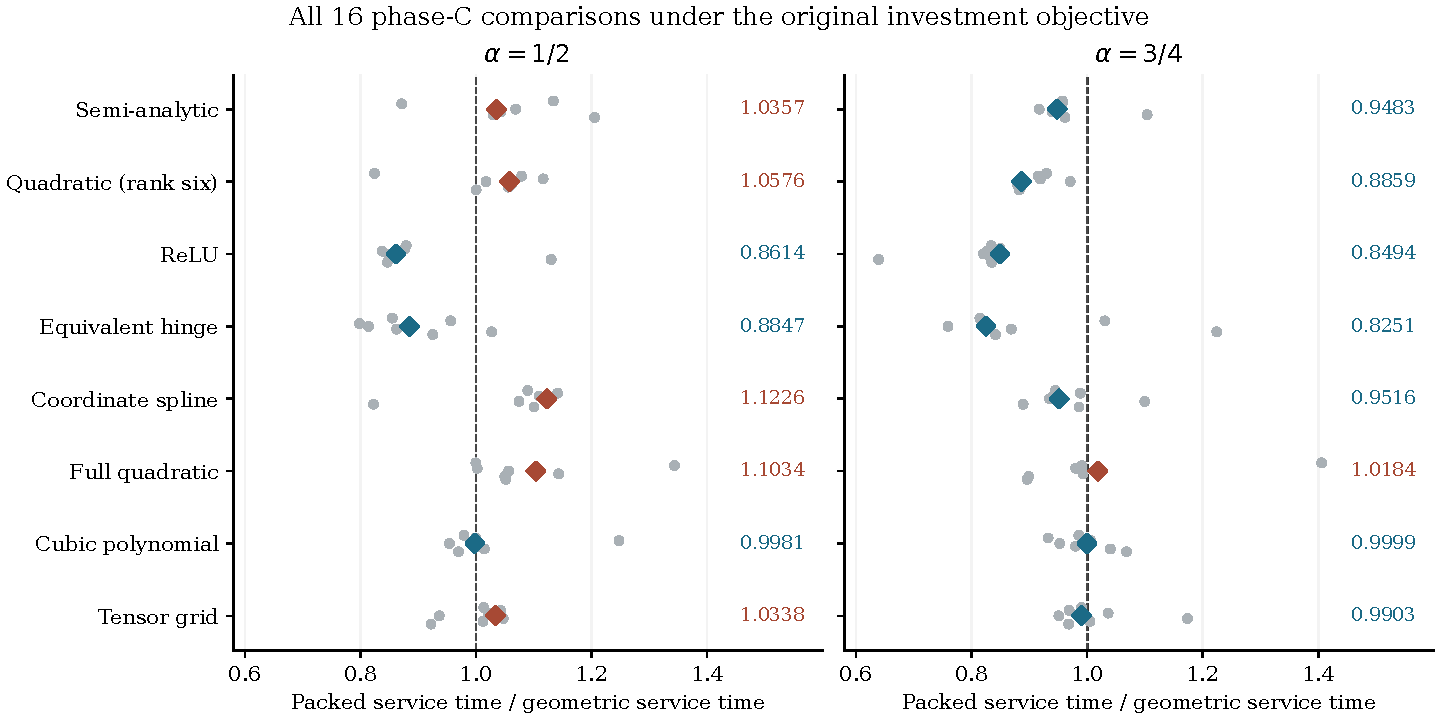
\includegraphics[width=\linewidth]{figures119/phase_c_all_clocks119.pdf}
\caption{All contemporaneous phase-C packed/geometric service comparisons.
Diamonds show the ratio of the two seven-process median times; grey points
show every paired process ratio. Values below one favor packing. These are
32-decision service clocks with actual loading and broader process costs
reported separately, not confidence intervals.}\label{fig:clocks119c}
\end{figure}

All 13,824 primary and 21,504 timing decisions completed.  The native
exact record audit passes 1,325,935 checks over 55,043 attempted
certificates; a separate read-only report verifies all 768 raw hashes
and 384,551 further exact/identity conditions.  An additional 21,974
read-only checks reconstruct the same original point coordinates for
the budgeted and fused services from their exact state, action, cut and
resolution records.  All 5,888 paired decisions use identical paid
preliminary information and qualification exits.  F uses 27 packed
compiler calls for the primary catalogue and 182 across the seven timing
processes, containing respectively 24,193 and 35,504 midpoint/endpoint
payloads.  The separate two-point defect calculation remains charged.
The 30-value general and 16-value boundary preliminary caps are attained
and respected.  Complete original risk-point queries remain 154,217,
exactly the budgeted service's count.

Table~\ref{tab:timing119c} reports the full contemporaneous comparison.
F is faster than B in all 16 median-clock cells, including 11 with all
seven paired clocks lower.  It is faster than C in all 16 medians, than
T in 14, and than G in ten.  The remaining six losses against G are
retained.  At $\alpha=1/2$, the ReLU ratio F/G is $0.8614$, with six
paired wins; at $3/4$ it is $0.8494$, with seven.  Conventional hinges
benefit similarly.  Quadratic at $1/2$ instead has ratio $1.0576$,
while quadratic at $3/4$ has ratio $0.8859$ and seven paired wins.
The degree-three polynomial ratios $0.9981$ and $0.9999$ illustrate
why a median win alone is weak evidence of a substantial advantage.
All ranges and every clock remain reported; no timing confidence
interval or architecture-independent speed guarantee is inferred.

Across all primary cells, F costs $6.5522$ seconds, compared with
$6.7726$ for G and $6.8250$ for B.  It is faster than G in 11 of 16
complete 144-state service cells and slower in five.  These totals
describe the entire predeclared tournament.  They do not construct a
new service by selecting the fastest implementation state by state.
The result identifies a practical part of the information-to-work
connection: the proved small payload budget becomes more competitive
when its many individual arrays are evaluated together.  Packing,
scattering, outward zero terms, attempted certificates and all fallback
work remain inside the measured boundary.

All fifteen within-arm service contrasts still have exactly the same
complete original policy at each of 2,304 state--risk--arm combinations.
Their original economic contrast is exactly zero.  Repacking changes
some outward endpoints---600 primary and 2,030 timing rows differ from
B---without changing their qualification exits or policies.  Original
regret and action-distance bounds retain their previous interpretation,
and no exact rational fallback is needed.  The 1,464 primary repairs
are the same 244 distinct proposals repaired under six services.

Representation-specific adoption remains unsupported.  Charging fresh
standalone acquisition and actual loading, quadratic with G costs
$0.1485$ seconds for the full $\alpha=1/2$ catalogue, versus $0.3407$
for ReLU with F.  At $3/4$, quadratic with F costs $0.1417$, versus
$0.3131$ for ReLU with F.  Quadratic also has the strictly lower
catalogue-mean original economic cost at both risks.  The ReLU--hinge
identity holds in all 96 paired files and 4,416 paired decisions,
including attempted certificates.  The conditional adoption inequality
in Section~\ref{sec:study119} therefore continues to require the full
resource and economic comparison, not an architecture label.  Phase C
adds a shared original-decision computational improvement while
preserving the negative A/B implementation findings, R97's adverse
acquisition result, and the still-open action-aligned learning and
larger-application obligations.

\subsection{Independent value enclosures for every recorded original policy}
\label{sec:study119d}
The 1,024-bin reference uses a separate whole-support risk partition with the
shared verified terminal compiler. To check original policy values through a
separate implementation, validation D was frozen at \texttt{cafd38ae}
after all A--C outcomes were known. It fixes 64 whole-support cells and up to 32
rational terminal bisections on every one of the 983 realized state/action/risk
keys represented by C's 13,824 primary decisions. The exact binary state and
action identities are retained. This is validation of the known catalogue.

The standard-library implementation reconstructs the original nonlinear
economic primitives, the terminal shock polynomial and its continuous AVaR
integral, and a feasible strong-convexity bracket for $V_1^*$. Conditional
Jensen bounds for $(V_1^*\circ F-\eta)_+$ and the repeated-endpoint secant
mixture give independent whole-support bounds for the original $Q$.
Proposition~\ref{prop:independentvalidation119} in the supplement proves these bounds.
Adding the unchanged $\beta 2^{-20}$ future-controller allowance once gives
the complete-policy $J$ enclosure. The production compiler is not imported.
This does not directly evaluate the deployed floating terminal controller or
independently determine the global date-zero regret optimum.

All 983 keys and 126,807 exact terminal contexts completed, with
652,774 recorded checks and no failed key.
The independent intervals overlap all 13,824 corresponding service intervals
and all 983 shared-compiler reference intervals. Overlap establishes
compatibility; it does not certify each fine reference endpoint merely from
intersection. All exact traces, checks and containment directions are retained.

\begin{table}[t]\centering\small
\caption{Independent Fraction original-policy mean-cost enclosures on the fixed catalogue.}\label{tab:independent119d}
\begin{tabular}{llrr}\hline
$\alpha$ & Representation & Lower mean cost & Upper mean cost \\ \hline
$1/2$ & Semi-analytic & 0.611452244 & 0.611454152 \\
$1/2$ & Quadratic (rank six) & 0.611604999 & 0.611606910 \\
$1/2$ & ReLU & 0.611623342 & 0.611625227 \\
$1/2$ & Equivalent hinge & 0.611623342 & 0.611625227 \\
$1/2$ & Coordinate spline & 0.611715940 & 0.611717849 \\
$1/2$ & Full quadratic & 0.611604999 & 0.611606910 \\
$1/2$ & Cubic polynomial & 0.611667314 & 0.611669224 \\
$1/2$ & Tensor grid & 0.611462422 & 0.611464314 \\
$3/4$ & Semi-analytic & 0.621104706 & 0.621106644 \\
$3/4$ & Quadratic (rank six) & 0.621266923 & 0.621268911 \\
$3/4$ & ReLU & 0.621285373 & 0.621287354 \\
$3/4$ & Equivalent hinge & 0.621285373 & 0.621287354 \\
$3/4$ & Coordinate spline & 0.621393664 & 0.621395613 \\
$3/4$ & Full quadratic & 0.621266925 & 0.621268914 \\
$3/4$ & Cubic polynomial & 0.621313002 & 0.621315001 \\
$3/4$ & Tensor grid & 0.621139623 & 0.621141543 \\
\hline\end{tabular}
\\[4pt]\parbox{.96\linewidth}{\footnotesize Each endpoint is an outward decimal display of an exact rational bound. Every mean weights the same 144 realized original states equally. All six services return exactly the same complete policy within an arm; all 96 arm/service/risk means are retained in the development companion. The future-controller allowance is $\beta 2^{-20}$. These intervals are numerical enclosures, not sampling confidence intervals.}
\end{table}


All 96 arm/service/risk means and all 56 arm contrasts are independently
reaggregated. There are 32 strictly negative, 20
strictly positive, 2 exact-zero and 2
unresolved contrast intervals in the fixed left-minus-right orientation.
The ReLU-minus-quadratic original mean-cost intervals are
$[17.4360, 19.2238]\times10^{-6}$
at $\alpha=1/2$ and
$[17.5331, 19.3595]\times10^{-6}$
at $\alpha=3/4$. The full contrast table retains every sign and exact tie.
These independent intervals confirm the rank-six quadratic arm has strictly lower mean original policy cost than ReLU at both risk levels. ReLU and its exactly equivalent conventional hinge representation retain identical realized policies and exact-zero mean cost contrasts.
All 240 arm/risk/service-pair cells have identical complete policies, preserving
the exact zero economic effect of changing only the certification service.
No favorable economic sign was a validation pass condition.

D requires 1697.332 seconds of additional actual
author-side validation time (1693.604 CPU seconds),
including its separately recorded binding, rational solves, primitive traces
and aggregation. This cost is reported separately from the unchanged A--C
acquisition and service clocks. D strengthens independent original-model value
evidence; it creates neither an unseen population result nor a neural-specific
adoption claim.

\section{Conclusion}\label{sec:conclusion119}
Neural Bellman Operators link recursively acquired continuations to feasible
original-objective decisions. The complete account includes the actor's own
future policy, action-dependent continuation error, original-law numerical
witnesses and the cost of obtaining them. The original construction and the
completed-policy safeguards establish precise decision guarantees without
assuming that an optimizer successfully trains an arbitrary network.

The present revision identifies the adverse innovation region as a paid
information decision. For scalar uniform risk and convex Lipschitz
continuations, locating that region before integration yields matching
deterministic bounds with linear tail-length dependence. The original
investment primitives turn an approximate location into an outward
all-action certificate, and a finite preliminary budget limits work spent
before the complete original solver is invoked. These contributions concern
the information and certification components of NBOs and are available to
all same-information representations.

The experiments distinguish information savings, service time and economic
loss. They retain every fixed-catalogue decision, every timing repetition,
all rejected certificates, independently paid references and the strong
conventional frontier. Equivalent ReLU and hinge actors receive equal
information and full acquisition charges. An unchanged complete policy has
unchanged original economic value. Computational adoption therefore requires
both a competitive complete service and a justified economic workload; a
smaller fitting residual or a smaller query count alone does not establish it.

The research program continues toward prospective action-aware acquisition,
neural-specific benefits under matched resources, larger dynamic economic
problems and calibrated use. The new proofs and executed algorithms make
those questions more sharply testable. The complete supplement states the
mathematical assumptions and proofs, while the development companion retains
the earlier applications, policy improvements, negative experiments, unresolved
claims and independent source identities needed to continue that program.

\section{Current execution and retained scientific identities}\label{dev:custody119}
This is the development companion of the R119 author revision. Its complete
native author baseline is R110, commit
\nolinkurl{4ba2bbaa11b5fa59f83705b28b35bf82a63ca169}; the controlling persisted
advisory is R97, commit \nolinkurl{9723c6cd2cc8b3e071422f3e522d4a843946db63},
which reviewed manuscript \nolinkurl{f802fe64d91d9f5c1c8f86123b0fbe114e622279}.
It is an owner-commissioned advisory, not an Econometric Society editorial
judgment on this revision. The R118 Git custody parent preserves the unchanged
R110 manuscript but does not establish a complete newer paper from its
truncated source transport. The scientific source and execution identities,
current figures, all reports and content-retention maps are supplied with the
referee-ready source package.

Historical occurrences of ``current'' and ``new'' below refer to the revision
that originally wrote that section. No historical table is relabeled as an
R119 observation. R98, R111--R118 and other independent experiments retain
their source, protocol, sampled-actor or execution constraints. Reproductions
are separately labeled and charged. The current main article states the
original NBO research question and current mathematical and empirical
contributions; this companion preserves the wider program and its evidence.


\subsection{Scientific episodes, observation scopes and actual work}
\label{dev:execution119}
The current work began by reading the branch trees, persisted reports,
complete manuscript dependencies and recorded experiment identities. The
reliable complete author source is R110, whose unchanged native dependency
closure was restored before the present additions. The independent R117 and
R118 programs were recovered under their own freezes. Their attributable
reproduction on this host preceded the new active-tail design. None of the
new deterministic investment catalogues supplies observations for R98's
selected-actor experiment, R115's independent sample/actor work, or another
uncompleted frozen episode. The source and episode maps retain the differing
status of protocol text, native manuscript dependencies, executed code,
missing observations and truncated transports.

\paragraph{Three successive current interventions.}
Phase A is bound to source commit
\nolinkurl{1f33c2667e0dff89699c6d6a01d03eacfecf3f4e}; phase B's actual successful
execution is bound to
\nolinkurl{357b2c56727cd57b9696cd6e07e115a35f5fdedb}; phase C is bound to
\nolinkurl{095936f1a7556d90d74809e63d75d9959d118360}.
Each phase has its own protocol, full source hash manifest, output directory,
preflight and recorded command. Phase A compares three services, phase B five
and phase C six. All eight representations and both risks are retained in
each contemporaneous tournament. The primary catalogue has 144 states per
cell. Seven sequential fresh processes each time 32 states per cell, with
the frozen rotated service order. Phase B was designed after the adverse A
clocks, and phase C after the adverse B overhead finding. They are separate
prospectively committed implementations on an already observed catalogue.
The earlier results remain observations of their original implementations.

\begin{center}\small
\begin{tabular}{lrrrr}
\toprule
Phase & Primary decisions & Timing decisions & Certificate attempts & Exact checks\\
\midrule
A & 6,912 & 10,752 & 25,161 & 444,053\\
B & 11,520 & 17,920 & 45,557 & 1,031,933\\
C & 13,824 & 21,504 & 55,043 & 1,325,935\\
\bottomrule
\end{tabular}
\end{center}
The complete current study thus retains 82,432 primary or timing decisions.
The record audits check every original-policy reference and 2,801,921 exact
conditions in aggregate. The 1,024-bin reference calculation uses an
independent integration partition but shares the verified terminal compiler
with production; the separately implemented exact-rational primitive audit
has the finite original-model scope specified below. Additional independent reporting checks have their
own ledgers and are not added as independent economic observations. All
three implementation preflights use the same previously declared 22,220
exact checks, including 880 constrained cases, 228 meshes, 24 original
references and 72 certificates. Repeating this known diagnostic suite is
implementation validation, not an independent sample. The supporting
rational tail comparison has 320 declared cells: active-tail width wins 242,
whole-support width wins 27 and 51 tie. This auxiliary exact family retains
its own scope and does not replace the original investment comparison.

\paragraph{Complete costs and the timing boundary.}
Every phase acquires labels and fits all competing representations afresh.
Standalone costs charge the complete common-information label acquisition
required by the arm, fitting and fit audits, actual model loading, attempted
certificates, rejected candidates and the complete decision fallback.
Independently paid policy references are reported separately from deployment
work. The catalogue totals do not select a fastest service after observing
each state. The acquisition, reference, primary service and fresh-process
clocks are all retained, so a user can assess a stated deployment workload.
The measured 32-decision service clock begins after its separately measured
model load; interpreter startup, source verification and the entire command
have broader recorded boundaries. They are not silently assigned to the
narrower clock. In phase C, all 112 timing loads and 16 primary loads are
retained, and the shared primary loading blocks total 0.000661019 seconds.
The complete 144-state component tables charge those actual primary loads.

The outer primary commands took 86.421052, 137.466462 and 155.932757 seconds
in phases A, B and C, respectively. Those commands include their stated
acquisition, campaign and output work and are not a reconstructed sum of
selected successful kernels. Source, process-start, serialization, supporting
audit and manuscript-production costs remain visible in their actual logs.
No clock has been rerun to remove an adverse observation or to create an
unobserved homogeneous machine comparison.

Phase A overlapped some author-side diagnostic work. Its primary command
ran from Unix time 1792300099.343158 to 1792300185.764407. A Pandoc conversion
has a file interval of about 0.284 seconds within that window; this is not
an inferred CPU-time measurement. The theory diagnostic and compilation
records also prevent an assertion of zero concurrent CPU activity. Their
saved actual timestamps are retained in the concurrency disclosures. Before
the B and C primary clocks, all author-side agents acknowledged pausing
local computation; the root used short status polling and remote operations.
These controls characterize this host's observation conditions and do not
establish an architecture-independent timing result.

\paragraph{Failure and repair custody.}
The first phase-B preflight stopped before scientific imports or observations:
the remote transfer of the phase-A frontier CSV had normalized CRLF bytes to
LF. The frozen local CSV has 23,044 bytes and SHA-256
\nolinkurl{2eb4b04a3bea1ee56fc849b81078656a3dac15c84afa1bdbd646f929413d0ef9}.
Restoring those exact declared bytes produced the successful custody commit
stated above. The algorithm, protocol, local data and freeze manifest were
unchanged. The failed attempt, its log and its nonzero exit code remain in
\nolinkurl{results119/independent_budgeted119}; the successful new attempt is
\nolinkurl{results119/independent_budgeted119-attempt02}. The source transport
failure in the earlier reproduction and a read-only phase-C reporter failure
are also retained under their actual scopes. A failed packaging or reporting
command is not an economic method observation; its repair does not erase it.
The first package-validation replay also correctly stopped at the native
auditor's existing-receipt guard. The wrapper was repaired to preserve the
original receipt copies in a separately named custody directory before
creating fresh replay receipts. Neither the archive nor any frozen scientific
source or observation was changed.

\paragraph{Attributable unchanged-source reproductions.}
The R117 reproduction retains 4,608 primary and 7,168 timing decisions, seven
fresh processes, 204,912 exact record checks, 3,072 independently implemented
primitive checks and 5,116 additional exact checks. The matched geometric
and compiled controls return the same complete policies. In this reproduction
geometric scheduling is slower in five of the sixteen median cells,
including both ReLU cells. The separately scoped R118 supporting quadratic
oracle reproduction has 792 cells, 41,403 exact checks and 26,136 exhaustive
actions; 352 strict minimax-regret improvements and 440 ties are retained.
Its quadratic function class, oracle and objective are explicitly different
from the investment tournament. Reproduction evidence is bound to custody
commit \nolinkurl{54512c9c7fcdc75d97ad37d20b8b61f22356a953}, and the older
R117/R118 source and protocol freezes remain in the episode ledger.

\paragraph{Historical byte and source coverage.}
The initial inventory records 359 remote heads, 301 distinct head commits,
and all relevant author, review, source, integrated, publication and evidence
lineages. Its reachable-object audit read and verified 1,595 commits and
13,676 trees. The available native scientific text included 32,067 distinct
\texttt{.tex}, \texttt{.py}, \texttt{.md} or \texttt{.json} blobs, totaling
519,606,982 bytes, plus 5,332 ancillary text blobs. It indexes 587 native
statement environments, 118 Markdown claims, 366 proof environments and
238 proof headings. This is a source-reading and traceability index; it does
not assert that every historical theorem has been independently reproved.
The original-correctness section below explicitly identifies several false
original statements and supplies the corrected result or counterexample.

The nonduplicating local raw audit then read every remaining 18,730 available
historical blob, totaling 1,249,738,781 bytes. It checked Git hashes throughout;
8,136 ZIP/NPZ bodies were inspected without unpickling, 10,590 opaque binaries
were fully hash-read, two gzip payloads and one TSV were parsed. The sole
semantic failure is the previously identified truncated R118 source transport;
its actual bytes still verify. No historical numerical program was executed
by this parser. The remaining remote-object manifest was then completely read by its local
streaming mirror: all 10,358 immutable objects, totaling 15,397,774,846
unique bytes, were hash-verified and format-audited. Nine HTTP 502 transport
failures remain in the attempt record; a separate retry-only manifest
completed all nine without redownloading a successful object. All 1,239
JSON and six JSONL bodies parsed. Four large field-frequency summaries
were completed from retained key events without replacing or redownloading
the underlying data.

The disjoint historical union excludes sixteen new-revision source objects
from the broad initial local index. It contains 37,383 original indexed
source/ancillary blobs, 18,730 available raw blobs and 10,358 originally
missing remote blobs: all 66,471 historical blobs reachable from the
original 359 heads, or 17,202,527,633 unique bytes. No expected object is
missing or replaced. Three historical Python syntax errors and the
truncated R118 archive remain explicit semantic defects. Opaque model,
pickle, PDF and image bytes are fully hash-read; this coverage is not a
claim to unpickle models or visually review every historical image.
The separate GitHub streaming run is not counted as a successful CI
execution on the strength of this completed local mirror.

\paragraph{Recovered complete R110 execution package.}
The original R110 artifact, identifier 12053947106 from successful original
run 38899876276, has 638,792,519 bytes and ZIP SHA-256
\nolinkurl{dff93fc7dbf82f7a36ffbfde0c9c74a7b8ebc1006e3fd72ba33927c065e430cb}.
The new custody-only run 39101786083 verified its 9,648 members and reproduced
a transport of the 9,636 non-cache member files. All 8,218 source-export
matches were exact, and all four originally logged PDF byte identities were
verified. The twelve omitted files are Python bytecode caches, all listed
in the receipt; no scientific source, raw outcome or failure was selected
away. The two downloaded transport artifacts were independently checked and
reassembled locally to the new selected ZIP with SHA-256
\nolinkurl{9f40a73a3ce4ca154228b1ffceb304be8a5a77d2909fc69b278fe0c56a94a8c2}.
A second independent local custody check verified all 9,636 selected files,
933,909,545 expanded bytes, all 9,635 original output-manifest hashes and
all 8,218 source-export SHA-256 and Git identities. The 5,097 JSON member
bodies were fully read: 2,915 unique contents received strict parsing and
2,182 exact-content repeats reused that parser result. All 3,751
source-export JSON identities and 5,096 execution-receipt members match.
Earlier progress snapshots still say ``running''; the complete final
campaign manifests, seven zero-exit timing processes per campaign and
final exact audits establish the completed episode. The snapshots are
preserved with their own time and meaning. These operations recover
original execution evidence. They do not rerun R110 or convert its
observations or remote elapsed clocks into current results.

\paragraph{Interpretation and continuing scientific requirements.}
All fifteen phase-C within-arm service contrasts have the same complete
policy at every matched state, hence exact zero original economic contrast.
Different outward payloads caused by batching do not alter that observed
policy identity. The shared packed service reduces actual certificate work
in ten of sixteen contemporaneous median cells against the geometric control;
all six losses and every clock are retained. Quadratic remains the stronger
complete component/economic comparison at both risks, and the conventional
hinge realizes the same ReLU geometry. Thus the current advance is a proved
original-risk information account and an executed decision-service improvement.
Prospective action-aligned learning, a neural-specific matched-resource
separation, longer learned horizons and calibrated application adoption still
require their own evidence. The original NBO research objectives and retained
credible results remain active; the present tables do not certify those
uncompleted scientific claims.

\section{Corrections to the original formulation and the retained research programme}
\label{dev:originalcorrection119}

This section records mathematical corrections to the original author source
\texttt{bf049e302e9ed38303084e8da16b13717b052a70}, identified in the
12 major comments of the report dated 15 September 2026.  The original files,
counterexamples, and subsequent numerical records remain in the immutable
development history.  Preservation of an original statement is not an
endorsement of its validity.  In particular, the original composite-loss
optimality proposition, residual-based viscosity-selection assertion, and
unverified equilibrium claims are not premises of any current theorem.
The current Bellman construction, actor comparison, and continuous-risk
certificates are stated and proved separately in the main text and supplement.
The following corrections are elementary diagnostics, not new contributions
or reruns of the original economic experiments.

\subsection{The original scalar loss and the current computational graph}
\label{dev:compositeloss119}

The original loss was
\[
 L(\pi,V)=-\mathbb E H^\pi[V]
       +\omega\mathbb E(-V_t-H^\pi[V])^2.
\]
Joint minimization does not force the second term to vanish.  For the
one-action, no-state problem with terminal value one at date one and
aggregator $f(v)=-v$, the correct solution is $V^*(t)=e^{t-1}$.
With uniform sampling and $\omega=1$, put
$V_\varepsilon(t)=V^*(t)-\varepsilon(1-t)$.
The terminal value is unchanged, whereas
\[
 -V_\varepsilon'+V_\varepsilon=-\varepsilon(2-t),\qquad
 L(V_\varepsilon)-L(V^*)
       =-\frac{\varepsilon}{2}+\frac{7\varepsilon^2}{3}.
\]
This difference is strictly negative for $0<\varepsilon<3/14$ and equals
$-3/112$ at $\varepsilon=3/28$.  Thus the claimed local, and hence global,
optimality assertion was false even with exact terminal data.  In the
stationary scalar case the same issue is the identity
\[
 -H+\omega H^2
   =\omega\left(H-\frac{1}{2\omega}\right)^2
      -\frac{1}{4\omega}.
\]
Its minimizer is not the Bellman root.

The current actor is proposed from a specified fitted continuation and
accepted only using the original objective and the stated independent
certificate.  The current critic fitting criterion has its own parameter
block.  Neither computation is justified by the false joint-loss proposition.
The supplement's computational-graph subsection following
Proposition~\ref{prop:investmentfoundations119} gives the full chain rule for
the criterion $\tfrac12\mathbb E r^2$, including generator and shared-parameter
channels, and states exactly when a detached continuation changes that
derivative.  A zero target or an automatic-differentiation implementation does
not prove optimizer stability, two-timescale convergence, or a utility
gradient under an arbitrary state-sampling law.

\subsection{Boundary data and viscosity selection}
\label{dev:viscosity119}

Zero interior residual does not choose terminal or lateral data: with zero
flow and dynamics, every constant has zero interior residual, while terminal
payoff zero selects only the zero constant.  Proposition~\ref{prop:finitefoundations119}
specifies the terminal function, admissibility, continuous Bellman class,
measurability, and policy recursion actually used in the current finite-horizon
model.  Proposition~\ref{prop:stoppedbsde119} specifies the separate Brownian
boundary/terminal discrepancy under stopping.  An infinite-horizon claim
additionally requires the stated function class and contraction or
transversality hypotheses; it does not follow from a finite-horizon argument.

Even exact boundary data and vanishing population squared residual do not
give a general viscosity-selection theorem.  For the deterministic exit
problem with speed in $[-1,1]$ and payoff minus elapsed time, the equation is
$1-|V'|=0$ on $(-1,1)$ with zero boundary values.  Its value is
$V^*(x)=|x|-1$.  The smooth functions
\[
 W_\varepsilon(x)=\sqrt{1+\varepsilon^2}
                      -\sqrt{x^2+\varepsilon^2}
\]
have the same boundary values and satisfy
\[
 \mathbb E\{1-|W_\varepsilon'|\}^2
 =2-2\sqrt{1+\varepsilon^2}+2\varepsilon
       -\varepsilon\arctan(1/\varepsilon)\longrightarrow0.
\]
Nevertheless, their uniform limit is $W(x)=1-|x|$.  The test function
$\varphi(x)=1$ touches $W$ from above at zero and gives
$1-|\varphi'(0)|=1>0$, violating the viscosity subsolution inequality.
The displayed integral follows by expanding the square on $[0,1]$ and
integrating $x/\sqrt{x^2+\varepsilon^2}$ and
$\varepsilon^2/(x^2+\varepsilon^2)$ separately.

The current results therefore do not identify spectral bias or fixed-network
training with vanishing viscosity.  Uniform action comparisons and coverage
allowances are explicit inputs to the current certificates.  A theorem on
approximating a smooth target and its derivatives does not approximate
nonexistent classical derivatives at a kink, prove optimization of a fixed
architecture, or provide a PDE comparison principle.

\subsection{Analytical portfolio and recursive-utility diagnostics}
\label{dev:mertonez119}

Under the original unconstrained Merton parameters
$(\mu,r,\gamma,\sigma,\rho)=(0.08,0.02,2,0.2,0.04)$, the formal stationary
CRRA benchmark is
\[
 \pi^*=\frac{\mu-r}{\gamma\sigma^2}=\frac34,\qquad
 m=\frac{\rho+(\gamma-1)
       [r+(\mu-r)^2/(2\gamma\sigma^2)]}{\gamma}
       =\frac{33}{800}.
\]
With $\mu=0.01$ the unconstrained allocation is $-1/8$ and its no-short-sale
projection is zero at every positive wealth level.  These values replace the
incorrect analytical numbers in the original table.  A finite horizon needs
its own terminal/bequest specification and generally does not have this
constant consumption ratio.  A control bound gives action-space optimality
conditions; it does not by itself create a wealth threshold, a value-gradient
jump, or an obstacle variational inequality.  The old constant-parameter
example consequently does not validate a switching-boundary claim.

For Epstein--Zin notation set $a=1-1/\psi$, $b=1-\gamma$, and $Y=bV>0$.
The originally printed aggregator was
\[
 f_{\rm old}(c,V)=\frac{\rho b}{a}c^aY^{1-a/b}-\rho V,
 \qquad (f_{\rm old})_c=\rho b c^{a-1}Y^{1-a/b}.
\]
It has negative consumption derivative when $b<0$, including the reported
$\gamma=5$ regime.  Under the conventional difference-form normalization,
the corrected expression is
\[
 f(c,V)=\frac{\rho}{a}
       \{c^a(bV)^{1-a/b}-bV\},\qquad
 f_c=\rho c^{a-1}(bV)^{1-a/b}>0
\]
for $c>0$ and $bV>0$.  The choice of normalization and its domain are part
of the model.  With the original return parameters, $\gamma=5$,
$\psi=3/2$, and $\rho=1/25$, formal stationary substitution gives
\[
 \pi=\frac3{10},\qquad
 m=\psi\rho+(1-\psi)
       \left[r+\frac{(\mu-r)^2}{2\gamma\sigma^2}\right]
       =\frac{91}{2000}.
\]
These algebraic identities are not an infinite-horizon existence or
verification theorem.  They do not establish integrability, admissibility,
selection of a recursive-utility solution, or preservation of the fractional
power domain by an arbitrary network.  The current bounded Lipschitz BSDE
bridge does not assert those properties for the singular Epstein--Zin
specification.  Current monetary-risk Bellman recursions and general nonlinear
recursive utility retain their different hypotheses and objectives.

\subsection{The expected stochastic-Hessian objective}
\label{dev:traceobjective119}

If $\widehat q$ is conditionally unbiased for the diffusion trace $q$, then
\[
 \mathbb E[(a-\widehat q/2)^2\mid a,q]
       =(a-q/2)^2+\tfrac14\operatorname{Var}(\widehat q\mid a,q).
\]
The conditioning here fixes the network, state, and all non-probe
quantities.  The variance usually depends on the network derivatives.
For one standard Gaussian probe with $\widehat q=hZ^2$ and $a=1$, Gaussian
second and fourth moments give $1-h+3h^2/4$, minimized at $h=2/3$, whereas
the true square is minimized at $h=2$.  Two conditionally independent probe
banks give the unbiased product
$\mathbb E[(a-\widehat q_1/2)(a-\widehat q_2/2)]=(a-q/2)^2$.
The individual product can be negative and its variance remains a numerical
cost.  For covariance $\sigma\sigma^\top$, a symmetric matrix actually
probed is $\sigma^\top D^2V\sigma$; for a nonsymmetric representation, the
quadratic form uses its symmetric part.  Unbiasedness of an unweighted trace
does not validate a diffusion-weighted implementation or a squared loss.
No current theorem concludes feasibility failure from trace noise when the
executed actor is hard-mapped into the feasible box.

\subsection{Preference control, temporal selves, and strategic deviations}
\label{dev:extensions119}

For the original additive preference diffusion
$U_t=u_0+\int_0^t\theta_s\,ds+\sigma W_t$, with $\sigma>0$ and
$|\theta_s|\le M$, one has $U_t\le u_0+Mt+\sigma W_t$.
Thus $\mathbb P(U_t<0)>0$ for every $t>0$ by the nonzero Gaussian lower
tail.  Bounded controls do not make the declared positive state invariant.
Moreover,
\[
 \partial_u\frac{c^{1-u}}{1-u}
   =\frac{c^{1-u}\{1-(1-u)\log c\}}{(1-u)^2}>0
       \quad(c>1,\ u>1).
\]
This calculation refutes the original sign argument; it does not determine
the derivative of the endogenous value.  Subtracting a term that varies
with a controlled preference state changes its rewards.  A boundary rule,
cardinal normalization, consumption units, and an observation model are
therefore indispensable to that research application.  Neither its FOC nor
a policy plot proves a comparative-static sign or econometric identification.
The original investment experiment in the main text does not replace the
independent two-dimensional validation still needed for this preference
model.

The original temporal-self Hamiltonian $\beta u(c)+V_x(r x-c)$ has local
FOC $\beta c^{-\gamma}=V_x$; for $\beta>0$, $\gamma>0$, and fixed $V_x>0$,
its solution $c=(\beta/V_x)^{1/\gamma}$ decreases with a lower $\beta$.
For comparison only, a specified one-step present-bias
objective $u(c)+\beta\delta V_{t+1}(F(x,c))$ instead has derivative
$u'(c)+\beta\delta V_{t+1}'(F)F_c$.  Neither algebra is a derivation of a
continuous-time sophisticated equilibrium.  A deviation must include its
effect on the state and continuation.  The original separate supplement's
$\sup_c\{u(c)-u(c^*)\}$ with all dynamics frozen fails that requirement.
The retained nonlinear-deviation result is explicitly conditional on the
specified recursive game and deviation class; slow target-network updates
alone do not establish subgame perfection.

For the Cournot diagnostic $u_i=q_i(1-q_i-q_j)$, the unilateral FOC is
$1-2q_i-q_j=0$ and the symmetric Nash choice is $q_i=1/3$.
Joint profit maximization permits $q_i=1/4$, where the unilateral derivative
is $1/4>0$.  Cross-player derivatives in a global scalar loss therefore
cannot be called unilateral best responses.  Exact evaluation of a policy
profile is also insufficient: exploitability requires a distinct best-response
comparison.  Finite-action certificates retain their finite action set;
continuous-game, equilibrium-existence, and large-market limits require
their own approximation, deviation, and market-scaling arguments.

Finally, the original plotting placeholders remain historical illustrations,
not observations or executed comparison runs.  New source hashes, protocols,
raw results, independent checks, and failures are identified by their own
execution episode.  None of the calculations in this section regenerates the
original portfolio, preference-control, temporal-self, or game experiment.

% Source-specific author responses, generated from the complete keyed map.

% Requires hyperref/xurl; no independent bibliography or document wrapper.

\section{Historical point-by-point author response}\label{dev:allreferee119}

This section gives a direct author treatment for every one of the 620 explicit major comment blocks in 34 substantive reports. It is part of the author revision, not an additional referee report. The 35th persisted document is the R50 threshold screen; R16 added no new report. The 620 blocks are not all 1146 hierarchical report sections, and additional actionable minor requests have a separate response. Exact original text, headings, report blobs, reviewed-source identities and complete current source hashes remain in \nolinkurl{HISTORICAL_CARRYFORWARD119.json} and the report registry. Each entry distinguishes an implemented author action from its remaining scientific requirement; no whole-report closure is implied.

\begingroup\small

Later validation D has its own prospective source commit \nolinkurl{cafd38aedc5bcbddf5aafee2481fbf5e9a267bab} and completed receipts. All 983 keys and 126,807 terminal contexts completed, with 652,774 recorded checks and no failed key. It independently encloses original values of the delivered C policies from Fraction economic primitives, without importing the production terminal compiler. It is post-C validation on the known catalogue, not new training, independent action selection, a global regret reimplementation, an unseen population or competitive retiming. Each affected response states its particular use and remaining boundary. Separately, the first historical-custody CI run has all sixteen jobs recorded as failed at checkout before auditing; the earlier partial-status snapshot and the guard-scope repair remain preserved. Actual final build and CI status are given by their own source-bound publication receipt.

\subsection{Initial report}

Original report: \nolinkurl{reviews/2026-09-15-econometrica/referee_report.md}. Review commit \nolinkurl{2fd3a5660e36e7e6a71abb4102480bdea03f6d9a}; report blob \nolinkurl{de747b0743a99bea9ce4ca29fe386c8800402b5f}.

\paragraph{R1. The proposed composite loss does not have the asserted correct minimizer}

We reproduce the terminal-preserving perturbation with loss decrease -epsilon/2+7 epsilon\textasciicircum{}2/3 and the stationary nonzero-root bias. The original joint-loss proposition is explicitly identified as false. The current actor proposal, critic objective and acceptance certificate use distinct specified computational graphs; the supplement includes every shared-parameter and generator derivative channel.

\par\emph{Remaining requirement.} This correction does not establish convergence of arbitrary jointly trained actor-critic optimizers or regenerate experiments claimed under the original false loss.

\par\emph{Current proof and action route.} \nolinkurl{new119/original_correctness119.tex}; \nolinkurl{new119/foundations_supplement.tex}; \nolinkurl{new110/core-main.tex}.

\paragraph{R2. The target boundary-value problem is not enforced, and its generality is overstated}

We now prove finite-horizon continuity, attainment, Borel policy selection and recursive policy evaluation under stated compact-domain, continuous-feasibility and risk-kernel hypotheses. The original investment domain is proved invariant by explicit algebra. The stopped Brownian proposition includes the terminal/\allowbreak{}lateral discrepancy and precise regularity and comparison assumptions.

\par\emph{Remaining requirement.} The compact monetary-risk theorem does not establish global CRRA/\allowbreak{}Epstein-Zin well-posedness on singular unbounded domains or close an arbitrary predictable covariance process into a Markov state.

\par\emph{Current proof and action route.} \nolinkurl{new119/foundations_supplement.tex}; \nolinkurl{new110/recursive_bridge.tex}.

\paragraph{R3. The viscosity-selection argument is not valid}

We include the smooth wrong-solution sequence for 1-|V prime|=0, its vanishing population squared residual and its viscosity-subsolution violation. Current certificates use uniform action comparisons with explicit coverage and boundary allowances. Neural spectral bias and fixed-architecture derivative approximation are no longer premises of a viscosity-selection claim.

\par\emph{Remaining requirement.} A general convergence theorem for learned degenerate HJB solvers still needs a consistent comparison-compatible approximation and control of training, sampling and actor-maximization errors.

\par\emph{Current proof and action route.} \nolinkurl{new119/original_correctness119.tex}; \nolinkurl{new119/active_tail_main.tex}; \nolinkurl{new110/action-main.tex}.

\paragraph{R4. The analytical validation is numerically wrong and the constrained test has no stated kink}

We correct the stationary analytical Merton values to risky share 3/4 and consumption ratio 33/800, and the constrained unconstrained share to -1/8 with projection zero at all positive wealth. We distinguish action-space KKT conditions from an obstacle problem; the current investment envelope explicitly differentiates the state-dependent feasible boundary.

\par\emph{Remaining requirement.} The historical Merton runs were not regenerated in R119; a genuinely switching continuous-time benchmark still requires its own horizon, terminal condition and independent solver.

\par\emph{Current proof and action route.} \nolinkurl{new119/original_correctness119.tex}; \nolinkurl{new119/foundations_supplement.tex}; \nolinkurl{new110/continuous-main.tex}.

\paragraph{R5. The source does not support the reported experimental evidence}

We explicitly classify the original constructed plotting curves as historical illustrations. Current numerical statements refer to frozen original-investment executions, raw outputs, independently checked records and source identities; the main text preserves traditional-method wins and distinguishes fresh runs from reproductions.

\par\emph{Remaining requirement.} The original placeholder DDPG, Merton and Cournot figures do not become observed evidence through preservation or through success of a different current experiment.

\par\emph{Current proof and action route.} \nolinkurl{new119/original_correctness119.tex}; \nolinkurl{new119/R119_STUDY_MAIN.tex}; \nolinkurl{appendix.tex}; \nolinkurl{PROTOCOL119.md}.

\paragraph{R6. The Epstein--Zin aggregator has incorrect monotonicity in the reported regime}

We show the negative marginal consumption derivative of the originally printed Epstein-Zin aggregator and give the corrected difference-form expression on c>0 and (1-gamma)V>0. The formal stationary values are 3/10 and 91/2000. The current BSDE result explicitly supplies its bounded Lipschitz and terminal assumptions instead of invoking a singular recursive-utility example as automatic coverage.

\par\emph{Remaining requirement.} A valid infinite-horizon Epstein-Zin verification and retraining in its precise parameter domain remain separate tasks; the formal candidate calculation is not that theorem.

\par\emph{Current proof and action route.} \nolinkurl{new119/original_correctness119.tex}; \nolinkurl{new110/recursive_bridge.tex}; \nolinkurl{new119/foundations_supplement.tex}.

\paragraph{R7. Zero-centered residuals do not imply stability, and the convergence proof does not cover the implementation}

We replace the zero-target intuition by the exact full derivative of a half-squared Bellman residual and identify the actor, critic and detached-continuation blocks. The finite recursion is validated independently of the optimizer, and policy acceptance is tied to a certified original-objective inequality.

\par\emph{Remaining requirement.} Constant-step Adam is not certified as a two-timescale scheme; off-policy state sampling is not automatically the occupation-weighted policy gradient, and generic optimizer stability remains unproved.

\par\emph{Current proof and action route.} \nolinkurl{new119/original_correctness119.tex}; \nolinkurl{new119/foundations_supplement.tex}.

\paragraph{R8. The NDU application has unresolved well-posedness and economic-content problems}

We prove that bounded drift cannot keep the original additive-Brownian preference state positive, correct the derivative of c\textasciicircum{}(1-u)/(1-u), and explain why state-dependent cardinal renormalization changes this controlled economy. Current investment invariance is proved separately and the earlier preference-control programme remains traceable.

\par\emph{Remaining requirement.} The original NDU model still needs its own viable state/\allowbreak{}boundary rule, justified normalization, independent two-state solver, comparative-static analysis and observation-based identification argument.

\par\emph{Current proof and action route.} \nolinkurl{new119/original_correctness119.tex}; \nolinkurl{new119/foundations_supplement.tex}; \nolinkurl{sections/supp70.tex}.

\paragraph{R9. The time-inconsistency extension is not a derived sophisticated-agent equilibrium}

We correct the local incentive calculation for beta u(c)+V\_x(rx-c), and explain why a deviation must change both current reward and future state. The inconsistent separate-supplement deviation expression is identified explicitly. The retained nonlinear-deviation theorem is conditional on a specified recursive game and deviation class.

\par\emph{Remaining requirement.} Slow target-policy updates do not prove sophisticated equilibrium; a single authoritative continuous-time preference kernel, extended equations and independent one-shot deviation tests remain necessary for that application.

\par\emph{Current proof and action route.} \nolinkurl{new119/original_correctness119.tex}; \nolinkurl{sections/recursive86.tex}; \nolinkurl{new119/foundations_supplement.tex}.

\paragraph{R10. The dynamic-game algorithm is not, as written, a Nash solver}

We give the exact Cournot distinction: symmetric Nash output 1/3, joint-profit output 1/4, and unilateral derivative 1/4 at the latter. Current derivative conventions separate player-specific objectives from a global scalar loss, and the conditional recursive deviation bound identifies the required best-response error.

\par\emph{Remaining requirement.} Finite-action game certificates do not prove continuous MPNE, equilibrium uniqueness, convergence of simultaneous learning, or a competitive limit without market-size scaling and independent best responses.

\par\emph{Current proof and action route.} \nolinkurl{new119/original_correctness119.tex}; \nolinkurl{sections/recursive86.tex}; \nolinkurl{new119/foundations_supplement.tex}.

\paragraph{R11. The scalability experiment does not identify a high-dimensional advantage, and novelty remains unisolated}

The constructive Bellman result now exposes its supplied features, purchased continuation information and exact ReLU/\allowbreak{}min-plus encoding. Equivalent hinge and classical polynomial/\allowbreak{}spline representations receive the same information and feasible decisions in the original-investment comparison, while the information lower bound states its oracle model.

\par\emph{Remaining requirement.} Structure-aware classical methods may win, as they do in important current comparisons. The two-dimensional experiment does not demonstrate a generic neural escape from high-dimensional control complexity.

\par\emph{Current proof and action route.} \nolinkurl{new110/core-main.tex}; \nolinkurl{new/decision99.tex}; \nolinkurl{new/information99.tex}; \nolinkurl{sections/supp70.tex}.

\paragraph{R12. Unbiased trace estimation creates a biased squared-residual objective}

We derive the variance term in the expected squared stochastic-trace loss, give the Gaussian h=2/3 versus h=2 counterexample, and state the independent-bank product correction. The matrix actually probed is specified as the diffusion-weighted symmetric matrix and derivative/\allowbreak{}covariance work must be charged.

\par\emph{Remaining requirement.} Unbiased product loss can have high variance and negative samples. No current theorem proves a universal dimension-proportional probe requirement or noise-induced violation of a hard feasible output map.

\par\emph{Current proof and action route.} \nolinkurl{new119/original_correctness119.tex}; \nolinkurl{new119/foundations_supplement.tex}; \nolinkurl{sections/supp70.tex}; \nolinkurl{new119/R119_STUDY_MAIN.tex}.

\subsection{Report R2}

Original report: \nolinkurl{reviews/2026-09-28-econometrica-numerical-methods-r2/referee_report.md}. Review commit \nolinkurl{278fb174eaee816259642675533a7281815a3df4}; report blob \nolinkurl{c0daf8f965292ca5dc7d3cf79c8857b8e8dce9c4}.

\paragraph{B1. The paper does not execute the numerical method it proposes}

The current manuscript specifies and executes the original Bellman problem with fitted future continuation, actor proposals and independent acceptance. Its constructive operator is identified mathematically rather than inferred from the existence of a generic nbo\_core module; executable arm and source identities are recorded for each experiment.

\par\emph{Remaining requirement.} This does not retroactively establish that the early generic actor-critic module generated the historical demonstration tables or prove end-to-end performance for every proposed extension.

\par\emph{Current proof and action route.} \nolinkurl{new110/core-main.tex}; \nolinkurl{sections/supp70.tex}; \nolinkurl{new119/R119_STUDY_MAIN.tex}.

\paragraph{B2. The manuscript does not isolate a novel numerical contribution against appropriate baselines}

We separate the classical Bellman/\allowbreak{}comparison foundations from the claimed method contribution: exact constructive representation, action-sensitive certification and continuous-tail information bounds. The original-law numerical study includes quadratic, polynomial, spline, equivalent hinge, grid and compiled alternatives with common information and complete decision-service costs.

\par\emph{Remaining requirement.} Current comparisons do not establish dominance over all Howard, direct HJB, DGM or BSDE implementations; those require model-matched, properly tuned experiments in their applicable PDE setting.

\par\emph{Current proof and action route.} \nolinkurl{new110/core-main.tex}; \nolinkurl{new109/compiler.tex}; \nolinkurl{new/information99.tex}; \nolinkurl{new119/R119_STUDY_MAIN.tex}.

\paragraph{B3. The proposed certificates are non-operational in the regime that motivates the paper}

The present policy certificate has explicit global lower and implemented-policy upper bounds, continuation error, action optimality and boundary terms. Tail allocation is an implementable source of a finite query bound, and the all-action support remains valid at action and tail boundaries.

\par\emph{Remaining requirement.} A learned monotone-scheme convergence assertion still needs the assumed training/\allowbreak{}discretization rates and coverage to be proved or measured; R119 does not infer them from small training loss.

\par\emph{Current proof and action route.} \nolinkurl{new110/action-main.tex}; \nolinkurl{new119/active_tail_main.tex}; \nolinkurl{new119/foundations_supplement.tex}.

\paragraph{B4. The endogenous-preference “reference” is dominated by arbitrary action truncation}

We retain the NDU action-grid expansion and its changed values as evidence that the admissible economic control set matters. The development correction separates a genuine model restriction from an innocuous numerical approximation and records the need for state-domain viability.

\par\emph{Remaining requirement.} A 27-action solution and a 175-action solution are different finite control problems unless a continuous-action error bound is supplied; the original continuous NDU optimum remains unvalidated by those comparisons.

\par\emph{Current proof and action route.} \nolinkurl{new119/original_correctness119.tex}; \nolinkurl{sections/supp70.tex}; \nolinkurl{appendix.tex}.

\paragraph{B5. The LQ experiment is a classical exact policy-iteration identity, not evidence of neural scalability}

The article explicitly distinguishes exact analytical or Riccati/\allowbreak{}Lyapunov calculations from neural training and counts the information provided to each representation. The present learned-continuation study is linked to its actual training data, policy decisions and work ledger.

\par\emph{Remaining requirement.} The historical analytical LQ identity is not a neural-training experiment or a demonstration of high-dimensional computational scaling.

\par\emph{Current proof and action route.} \nolinkurl{new110/core-main.tex}; \nolinkurl{new/information99.tex}; \nolinkurl{new119/R119_STUDY_MAIN.tex}; \nolinkurl{sections/supp70.tex}.

\paragraph{B6. The principal economic extensions are specified but not numerically delivered}

The current supplement provides the conditional recursion by which policy-evaluation and unilateral deviation errors enter an economic loss bound. Original game, temporal-self and preference-control source material is retained with its own objective and evidence status.

\par\emph{Remaining requirement.} Unexecuted extensions still require an independent best-response/\allowbreak{}equilibrium or control computation; investment results cannot be substituted for them.

\par\emph{Current proof and action route.} \nolinkurl{new119/original_correctness119.tex}; \nolinkurl{sections/recursive86.tex}; \nolinkurl{sections/supp70.tex}.

\paragraph{B7. The revision is too broad for the depth of result it currently provides}

The main argument now runs from a specified economic Bellman problem through constructive continuation representation, action certificate, continuous-risk algorithm and measured original-objective decisions. Earlier development is retained in the companion and source map, with explicit unresolved application requirements.

\par\emph{Remaining requirement.} A coherent presentation does not itself establish every ambition in the retained broader NDU, FBSDE, game and high-dimensional research programme.

\par\emph{Current proof and action route.} \nolinkurl{ECTA.tex}; \nolinkurl{new110/core-main.tex}; \nolinkurl{new110/continuous-main.tex}; \nolinkurl{new119/R119_STUDY_MAIN.tex}.

\paragraph{M1. The continuous-time verification theorem is useful but highly conditional}

We state exact admissibility, value-class, terminal and stopped-boundary hypotheses, and prove the finite-horizon original model satisfies its domain assumptions. The BSDE residual proposition distinguishes bounded C1,2 verification from a generic smooth-network heuristic.

\par\emph{Remaining requirement.} These conditions do not validate unbounded singular CRRA/\allowbreak{}Epstein-Zin claims without their additional integrability, comparison and transversality analysis.

\par\emph{Current proof and action route.} \nolinkurl{new119/foundations_supplement.tex}; \nolinkurl{new110/recursive_bridge.tex}; \nolinkurl{new119/original_correctness119.tex}.

\paragraph{M2. The viscosity theorem does not analyze the learned algorithm}

The current results distinguish finite Bellman validation and certified approximation from the convergence of a learned monotone PDE scheme. The original residual-to-viscosity shortcut is corrected with an explicit counterexample.

\par\emph{Remaining requirement.} Density of network classes does not prove that the implemented optimizer reaches the scheme accuracy required as the discretization scale vanishes.

\par\emph{Current proof and action route.} \nolinkurl{new119/original_correctness119.tex}; \nolinkurl{new119/foundations_supplement.tex}; \nolinkurl{new/information99.tex}.

\paragraph{M3. The repository does not implement the full acceptance procedure described in the paper}

The all-action lower support and implemented-policy upper bound make acceptance concrete, including feasibility, continuation allowance and tail integration. The compiler supplies a strong classical certifying reference rather than an unspecified global residual oracle.

\par\emph{Remaining requirement.} A generic nonlinear HJB/\allowbreak{}global-domain oracle is not furnished automatically; certification claims are restricted to the mathematical and numerical interfaces actually established.

\par\emph{Current proof and action route.} \nolinkurl{new110/action-main.tex}; \nolinkurl{new119/active_tail_main.tex}; \nolinkurl{new109/compiler.tex}; \nolinkurl{new109/improvement.tex}.

\paragraph{M4. The stochastic-trace result is disconnected from the experiments and tests}

The correction explains both the unbiased independent-bank identity and its remaining variance, distinguishing an algebraic identity from an executed training method. Current numerical claims use their real executed estimators and exact or outward checks.

\par\emph{Remaining requirement.} The independent-probe identity alone is not evidence of stable critic training or favorable end-to-end computational cost in a high-dimensional diffusion.

\par\emph{Current proof and action route.} \nolinkurl{new119/original_correctness119.tex}; \nolinkurl{sections/supp70.tex}; \nolinkurl{new119/R119_STUDY_MAIN.tex}.

\paragraph{M5. Reproducibility is improved, but the durable evidence package is incomplete}

Source and evidence custody is now based on immutable commit and blob identity, full raw records, original negative outcomes and actual CI status. The historical object audit distinguishes source reads, binary hash checks, parsing failures and newly recovered evidence. The first R119 historical-custody CI attempt is now preserved as an actual failure: the final saved job endpoint shows all sixteen jobs failed at checkout before their audit steps. The earlier twelve-failed/\allowbreak{}four-queued snapshot remains preserved as an earlier observation. Their job-wide no-lazy-fetch setting blocked promisor checkout; the guard is confined to the audit command at the D freeze. This repair is not itself a successful rerun, and the completed local byte audit is separate evidence.

\par\emph{Remaining requirement.} Conversation summaries, queued workflows and a source file without generated outputs are not substitutes for a completed reproducible historical run.

\par\emph{Current proof and action route.} \nolinkurl{provenance/historical/ci_attempt01/FINAL_JOB_STATUS119.json}; \nolinkurl{provenance/historical/ci_attempt01/JOB_STATUS_AND_DIAGNOSIS119.json}; \nolinkurl{provenance/historical/ci_attempt01/job-117605227246.log}; \nolinkurl{appendix.tex}.

\paragraph{M6. The method's name and operator interpretation need sharper definition}

The main text gives the Bellman map with domain, target and the continuation actually supplied to each actor, and separately defines its constructive representation. The supplement proves recursion and feasible selector existence for the current economic state space.

\par\emph{Remaining requirement.} The learned representation is not a new Bellman principle, and exact closure under supplied features does not remove the cost of obtaining those features.

\par\emph{Current proof and action route.} \nolinkurl{new110/core-main.tex}; \nolinkurl{sections/supp70.tex}; \nolinkurl{new119/foundations_supplement.tex}.

\subsection{Report R6}

Original report: \nolinkurl{reviews/2026-09-29-econometrica-numerical-methods-r6/referee_report.md}. Review commit \nolinkurl{998dc1bb9b2049080dcd2e21d543dcbee55cb4dc}; report blob \nolinkurl{7484c580a9bf512e2e48e4f105fc6f36f1f307d4}.

\paragraph{B1. The paper still does not isolate a numerical advantage or distinct capability of NBO}

We preserve the earlier direct-policy wins and use explicit equal-information/\allowbreak{}equal-feasible-policy controls in the current investment study. The main text reports the neural actor against quadratic, polynomial, spline and equivalent-hinge alternatives, with original economic objectives and paid service work.

\par\emph{Remaining requirement.} No neural incremental value is claimed from verifier availability or a shared feature geometry; current neural adoption remains conditional on an economic and complete-cost advantage actually demonstrated.

\par\emph{Current proof and action route.} \nolinkurl{new119/R119_STUDY_MAIN.tex}; \nolinkurl{new/decision99.tex}; \nolinkurl{sections/supp70.tex}.

\paragraph{B2. The only full economic certificate is one-dimensional and problem-specific}

The action-direction and coupled comparison results address the looseness of a scalar function-norm certificate. The tail theorem adds explicit continuous-risk query accuracy and the investment theorem an implemented-policy regret enclosure.

\par\emph{Remaining requirement.} The historical one-dimensional interval bound remains as observed; neither it nor the current two-dimensional service experiment certifies arbitrary multidimensional PDE boxes.

\par\emph{Current proof and action route.} \nolinkurl{new110/action-main.tex}; \nolinkurl{new119/active_tail_main.tex}; \nolinkurl{new/information99.tex}.

\paragraph{B3. The endogenous-preference NBO fails its own policy criterion and is platform-sensitive}

The R6 NDU cases that failed the declared 0.1 requirement and the superior direct/\allowbreak{}classical results are retained with their native records and environment identities. Current original-investment experiments use separate protocols and are not described as repairing those failed NDU runs.

\par\emph{Remaining requirement.} Cross-platform numerical differences and the original NDU target failure are not erased by later qualitative agreement or a different model meeting a new threshold.

\par\emph{Current proof and action route.} \nolinkurl{sections/supp70.tex}; \nolinkurl{new119/R119_STUDY_MAIN.tex}; \nolinkurl{appendix.tex}.

\paragraph{B4. The high-dimensional experiment measures local residual fitting, not value accuracy or scalability}

The supplement separates critic error, policy-value comparison, boundary/\allowbreak{}exit discrepancy and recursive occupation transfer. The new finite-horizon investment experiment has an algebraically invariant domain and independently enclosed original objective.

\par\emph{Remaining requirement.} The historical high-dimensional diffusion still needs a bounded weak-discretization error, coverage of escaped states and an independent policy-quality bound; residual passage is insufficient.

\par\emph{Current proof and action route.} \nolinkurl{sections/recursive86.tex}; \nolinkurl{new119/foundations_supplement.tex}; \nolinkurl{sections/supp70.tex}.

\paragraph{B5. The dynamic Cournot calculation is not evidence for the neural method}

We retain finite-action Cournot results under their finite action sets and make unilateral deviation error explicit in the recursive game statement. The original global-loss/\allowbreak{}Nash confusion is corrected algebraically.

\par\emph{Remaining requirement.} Zero exploitability on a finite grid is not neural learning evidence or a certificate for a continuous-action dynamic game without an action-approximation allowance.

\par\emph{Current proof and action route.} \nolinkurl{new119/original_correctness119.tex}; \nolinkurl{sections/recursive86.tex}; \nolinkurl{sections/supp70.tex}.

\paragraph{B6. The baseline study is still too narrow for the venue}

The current original-law comparison uses neural, quadratic/\allowbreak{}polynomial, spline, equivalent hinge, grid and an analytic compiler, with the same acquired data and explicit resource accounting. Strong classical wins remain in the principal economic results.

\par\emph{Remaining requirement.} This suite does not by itself cover every well-tuned PDE/\allowbreak{}BSDE method on every historical application; matching the underlying model and error target remains required.

\par\emph{Current proof and action route.} \nolinkurl{new119/R119_STUDY_MAIN.tex}; \nolinkurl{sections/supp70.tex}; \nolinkurl{new109/compiler.tex}.

\paragraph{B7. The paper remains too broad relative to its completed result}

The main article is organized around one complete Bellman economic problem, a constructive method, an executable certificate and observed policy/\allowbreak{}cost outcomes. The broader programme and negative evidence are preserved with their mathematical interfaces and unresolved requirements.

\par\emph{Remaining requirement.} Presentation coherence does not turn incomplete game, endogenous-preference or high-dimensional experiments into completed applications.

\par\emph{Current proof and action route.} \nolinkurl{ECTA.tex}; \nolinkurl{new110/continuous-main.tex}; \nolinkurl{new110/core-main.tex}; \nolinkurl{new119/R119_STUDY_MAIN.tex}.

\paragraph{M1. Recast the interval result as a conditional verified enclosure, not an independently certified theorem of execution}

We state the binary64/outward-arithmetic contract and separately include exact rational examples and independent primitive checks. Feasible tail densities and action supports are constructed with explicit dyadic and continuation allowances.

\par\emph{Remaining requirement.} A conditional floating-point enclosure is not a formally verified implementation of the whole runtime; arithmetic replay and independent algorithmic derivation remain different kinds of evidence.

\par\emph{Current proof and action route.} \nolinkurl{sections/supp70.tex}; \nolinkurl{new119/active_tail_main.tex}; \nolinkurl{new119/foundations_supplement.tex}.

\paragraph{M2. Define reproducibility at the level actually obtained}

The package distinguishes source reproducibility, actual execution recovery, arithmetic replay and empirical robustness. Historical platform-sensitive values keep their source/\allowbreak{}environment identity rather than being relabeled bitwise reproductions.

\par\emph{Remaining requirement.} Matching signs or broad patterns across platforms does not imply identical policy arrays, costs or confidence statements.

\par\emph{Current proof and action route.} \nolinkurl{appendix.tex}; \nolinkurl{sections/supp70.tex}; \nolinkurl{PROTOCOL119.md}.

\paragraph{M3. Report target selection and robustness more explicitly}

The current protocol states policy regret and objective interval tolerances in the original investment cost units; the article reports what each tolerance means for an accepted economic decision. Full cost and regret are displayed together.

\par\emph{Remaining requirement.} Older 0.1/0.2 utility or profit targets cannot be interpreted as percentages or economically small welfare losses without their own normalization and application argument.

\par\emph{Current proof and action route.} \nolinkurl{new110/continuous-main.tex}; \nolinkurl{new119/R119_STUDY_MAIN.tex}; \nolinkurl{PROTOCOL119.md}.

\paragraph{M4. Keep every continuous/\allowbreak{}discrete bridge visibly conditional}

Each transfer now names its continuous/\allowbreak{}discrete objective, policy class, terminal or boundary discrepancy and error terms. In the current invariant investment model, implementation and continuum-risk errors are explicitly enclosed.

\par\emph{Remaining requirement.} An unknown Euler, truncation or model-transfer error remains unknown; it is not set to zero by a confidence interval for a different discrete experiment.

\par\emph{Current proof and action route.} \nolinkurl{new110/recursive_bridge.tex}; \nolinkurl{new119/foundations_supplement.tex}; \nolinkurl{sections/recursive86.tex}; \nolinkurl{new110/continuous-main.tex}.

\paragraph{M5. The coupled-capital payoff diagnostic needs a designed error decomposition}

We separate policy comparison from critic fit and derive signed recursive contrasts under the original common risk law. The Brownian supplement exposes the boundary and discretization-related quantities needed before a path comparison can support a continuous-time objective claim.

\par\emph{Remaining requirement.} Historical Monte Carlo bias, extrapolation and state-coverage gaps are not retrospectively filled by the new deterministic investment comparison.

\par\emph{Current proof and action route.} \nolinkurl{sections/recursive86.tex}; \nolinkurl{new119/coupled_main.tex}; \nolinkurl{new119/foundations_supplement.tex}; \nolinkurl{sections/supp70.tex}.

\paragraph{M6. Compare computational work at matched accuracy}

The current work ledger includes acquisition, feature construction, training, rejected candidates, certification and inference, and evaluates complete decision services under declared protocols. The budget theorem links stopping to certified remaining economic gain.

\par\emph{Remaining requirement.} A raw optimizer step count or fast forward pass is not a matched-accuracy total-cost comparison; unused hardware or derivative work cannot be silently excluded.

\par\emph{Current proof and action route.} \nolinkurl{new119/R119_STUDY_MAIN.tex}; \nolinkurl{PROTOCOL119.md}; \nolinkurl{sections/supp70.tex}; \nolinkurl{new110/budget.tex}.

\paragraph{M7. Separate mathematical synthesis from genuinely new results}

We assign classical ownership to existence, contraction, comparison and monotonicity foundations. The methodological claims are the exact specified construction, action-aligned interface and continuous-tail information/\allowbreak{}precision results, each with a complete proof and equal-information scope.

\par\emph{Remaining requirement.} A standard verification theorem or generic network approximation statement is not claimed as neural-specific novelty.

\par\emph{Current proof and action route.} \nolinkurl{new110/core-main.tex}; \nolinkurl{new119/active_tail_main.tex}; \nolinkurl{new/information99.tex}; \nolinkurl{new119/foundations_supplement.tex}.

\paragraph{M8. Tighten the main text}

Current principal contributions and economic results appear in a compact main narrative, while complete proofs, earlier diagnostics and negative outcomes remain in a traceable development companion and immutable source index.

\par\emph{Remaining requirement.} Archival retention does not imply every historical theorem is valid; the original corrigendum explicitly records the known false propositions.

\par\emph{Current proof and action route.} \nolinkurl{ECTA.tex}; \nolinkurl{appendix.tex}; \nolinkurl{sections/supp70.tex}.

\paragraph{M9. Freeze the candidate before the review run}

New scientific episodes have their own frozen source and protocol identities and are only reported as executed when raw outputs and checks exist. The authoritative package and CI reference the actual immutable content, with failures retained. The D protocol, complete key catalogue and scientific sources were pushed at the recorded prospective cafd38aedc5bcbddf5aafee2481fbf5e9a267bab commit before evaluation. Its runtime binds all 49 scientific/\allowbreak{}source-control files first. The historical-custody CI's actual checkout failures remain archived and are not relabeled as a passed freeze or successful numerical execution.

\par\emph{Remaining requirement.} A workflow running against a moving branch or incomplete manuscript is not made referee-ready by a large version number.

\par\emph{Current proof and action route.} \nolinkurl{provenance/historical/ci_attempt01/FINAL_JOB_STATUS119.json}; \nolinkurl{provenance/historical/ci_attempt01/JOB_STATUS_AND_DIAGNOSIS119.json}; \nolinkurl{provenance/historical/ci_attempt01/job-117605227246.log}; \nolinkurl{appendix.tex}.

\subsection{Report R7}

Original report: \nolinkurl{reviews/2026-10-03-econometrica-numerical-methods-r7/referee_report.md}. Review commit \nolinkurl{c63f6817f498e1cfe9a653139f7a25bf44a4418a}; report blob \nolinkurl{3f56f9d86c6e1147cf3bf61f14f2580804fbc0f4}.

\paragraph{B1. There is no integrated R7 paper to referee}

R119 materializes an integrated main article, full supplement and development companion from content-verified author sources, rather than treating a protocol or evidence branch as a newer completed article. Source and PDF hashes identify the actual review object.

\par\emph{Remaining requirement.} The R7 evidence-only snapshot remains an incomplete historical manuscript handoff; later integration does not alter what was available at that review date.

\par\emph{Current proof and action route.} \nolinkurl{ECTA.tex}; \nolinkurl{supp.tex}; \nolinkurl{appendix.tex}.

\paragraph{B2. The actor is trained by an exhaustive action oracle, so the main capability claim remains unisolated}

The constructive operator and numerical protocol disclose which continuation values and action labels are acquired, and charge their computation before fitting or compression. Equivalent hinge and classical encodings receive the same features and all feasible proposals are assessed against the original Bellman objective.

\par\emph{Remaining requirement.} Compressing a precomputed all-action table does not establish that the actor solved an information problem inaccessible to the table or its classical representation.

\par\emph{Current proof and action route.} \nolinkurl{new110/core-main.tex}; \nolinkurl{sections/supp70.tex}; \nolinkurl{new/information99.tex}; \nolinkurl{new119/R119_STUDY_MAIN.tex}.

\paragraph{B3. R7 still does not establish a numerical advantage over direct or classical methods}

The historical NDU guard, direct and classical timings and losses remain separate observed results, including the classical advantage. The current compiler and geometric certificate serve as strong traditional controls for the new original-investment service.

\par\emph{Remaining requirement.} A post-review Chebyshev proposal is not a completed R7 result, and the later investment algorithm does not overturn the measured NDU ranking.

\par\emph{Current proof and action route.} \nolinkurl{sections/supp70.tex}; \nolinkurl{new109/compiler.tex}; \nolinkurl{new119/R119_STUDY_MAIN.tex}; \nolinkurl{appendix.tex}.

\paragraph{B4. The finite-model guarantees do not transfer to the stated continuous economies}

The manuscript distinguishes finite-grid NDU and game objectives from continuous control and states the extra action, interpolation and dynamics allowances needed for transfer. The current original continuous-risk investment certificate supplies those terms for its own model.

\par\emph{Remaining requirement.} Previously null continuous-action or time-discretization error entries remain unresolved for the historical NDU and game calculations.

\par\emph{Current proof and action route.} \nolinkurl{new119/original_correctness119.tex}; \nolinkurl{sections/recursive86.tex}; \nolinkurl{sections/supp70.tex}.

\paragraph{B5. The high-dimensional coverage study is a policy-evaluation diagnostic, not an optimality or scalability result}

The signed comparison theorem targets policy differences under a common original law rather than relying on unrelated value or coverage diagnostics. The boundary-aware Brownian result states the terms required to transfer a path comparison.

\par\emph{Remaining requirement.} Broader simulated state coverage alone does not bound weak Euler bias or establish proximity to the optimal high-dimensional continuous-time policy.

\par\emph{Current proof and action route.} \nolinkurl{new119/coupled_main.tex}; \nolinkurl{sections/recursive86.tex}; \nolinkurl{new119/foundations_supplement.tex}; \nolinkurl{sections/supp70.tex}.

\paragraph{B6. The independent interval replay strengthens only the one-dimensional result}

We distinguish independent arithmetic evaluation of fixed weights and cover geometry from independent policy derivation or fresh cover construction. R119 includes rationally checkable primitive identities and original-objective intervals, with their execution identities separate from production binaries.

\par\emph{Remaining requirement.} The historical one-dimensional mpmath replay is not a new multidimensional global certificate, and a faster direct replay remains a valid traditional win.

\par\emph{Current proof and action route.} \nolinkurl{sections/supp70.tex}; \nolinkurl{new119/active_tail_main.tex}.

\paragraph{B7. The paper remains too broad relative to its established contribution}

The article now links original Bellman learning, exact construction, action certification and measured economic service in one principal argument. Earlier experimental breadth is retained through its own source and unresolved scientific questions.

\par\emph{Remaining requirement.} The preserved breadth is a research programme, not evidence that each historical extension has a completed independent numerical validation.

\par\emph{Current proof and action route.} \nolinkurl{ECTA.tex}; \nolinkurl{new110/core-main.tex}; \nolinkurl{new110/continuous-main.tex}; \nolinkurl{appendix.tex}.

\paragraph{M1. Make the training oracle explicit in the algorithm and title}

Training data and supplied all-action information are explicitly identified as paid Bellman acquisition. The information theorem specifies the oracle, and the current study reports equivalent classical use of the same labels.

\par\emph{Remaining requirement.} Supervised imitation of a fully enumerated action oracle cannot be called avoidance of that enumeration in training.

\par\emph{Current proof and action route.} \nolinkurl{new110/core-main.tex}; \nolinkurl{sections/supp70.tex}; \nolinkurl{new/information99.tex}; \nolinkurl{PROTOCOL119.md}.

\paragraph{M2. Treat the raw actor as the primary neural result}

The current record distinguishes the proposed actor, accepted candidate, rejected proposals, repaired decisions and final service policy. It accounts for acquisition and certification before reporting deployment or representation cost.

\par\emph{Remaining requirement.} Historical raw-actor passage does not erase the memory and oracle work needed to produce or validate a guarded/\allowbreak{}shortlisted service.

\par\emph{Current proof and action route.} \nolinkurl{new119/R119_STUDY_MAIN.tex}; \nolinkurl{new109/improvement.tex}; \nolinkurl{sections/supp70.tex}; \nolinkurl{PROTOCOL119.md}.

\paragraph{M3. Separate training, oracle construction, verification, and deployment costs}

The complete-cost comparison includes target construction, feature generation, critic/\allowbreak{}actor fitting, certificate construction, rejected candidates and inference. Paid stopping is tied to a remaining original-objective gain bound rather than an internal fit score.

\par\emph{Remaining requirement.} A deployment-only timing or uncharged target kernel cannot justify adoption against a complete classical service.

\par\emph{Current proof and action route.} \nolinkurl{new119/R119_STUDY_MAIN.tex}; \nolinkurl{PROTOCOL119.md}; \nolinkurl{new110/budget.tex}; \nolinkurl{sections/supp70.tex}.

\paragraph{M4. Explain missing one-step pure equilibria}

The game statement specifies unilateral best-response error and retains finite-action outcomes, including nodes without a pure equilibrium when recorded. The original global-profit/\allowbreak{}Nash error is corrected with an exact counterexample.

\par\emph{Remaining requirement.} A minimum-defect pure pair is not an exact equilibrium; mixed-action existence and continuous-game transfer need their own computation and proof.

\par\emph{Current proof and action route.} \nolinkurl{new119/original_correctness119.tex}; \nolinkurl{sections/recursive86.tex}; \nolinkurl{sections/supp70.tex}.

\paragraph{M5. Add a true paired method comparison to the coverage audit}

Current same-law contrasts use coupled quantities and signed recursive propagation, and prospective stochastic comparisons must state their paired sample design. Historical comparisons retain the actual use or absence of common Brownian paths.

\par\emph{Remaining requirement.} The new deterministic investment comparisons are not retrospective confidence intervals for historical diffusion policies, training seeds or Euler approximations.

\par\emph{Current proof and action route.} \nolinkurl{new119/coupled_main.tex}; \nolinkurl{sections/recursive86.tex}; \nolinkurl{sections/supp70.tex}; \nolinkurl{PROTOCOL119.md}.

\paragraph{M6. Calibrate the error targets economically}

Current tolerances and objective differences are reported in the original model units, with regret and action error alongside work. Earlier absolute utility and profit thresholds retain their stated normalization.

\par\emph{Remaining requirement.} An absolute loss of 0.1 or 0.2 cannot be called a percentage or economically negligible without an explicit welfare-unit conversion.

\par\emph{Current proof and action route.} \nolinkurl{new119/R119_STUDY_MAIN.tex}; \nolinkurl{new110/continuous-main.tex}; \nolinkurl{sections/supp70.tex}.

\paragraph{M7. Use precise terminology for interval verification}

The evidence map distinguishes the exact fixed weights, cover, rounding contract and arithmetic implementation used in a replay. Independent rational primitive checks in R119 are reported under their own diagnostic protocol.

\par\emph{Remaining requirement.} Replaying a previously chosen interval cover with different arithmetic does not independently validate how that cover was selected or make the entire numerical stack formally verified.

\par\emph{Current proof and action route.} \nolinkurl{sections/supp70.tex}; \nolinkurl{new119/active_tail_main.tex}; \nolinkurl{appendix.tex}.

\paragraph{M8. Do not count the development protocol as completed baseline evidence}

Every new treatment is attached to a source and protocol frozen before its own run, and earlier proposed but unexecuted gated/\allowbreak{}Chebyshev work retains that status. Phase-specific results and failures are not pooled into a fictitious original preregistration.

\par\emph{Remaining requirement.} Post-primary proposals cannot be inserted into an earlier experiment's confirmatory denominator or called prospectively chosen there.

\par\emph{Current proof and action route.} \nolinkurl{PROTOCOL119.md}; \nolinkurl{PROTOCOL119B.md}; \nolinkurl{PROTOCOL119C.md}; \nolinkurl{appendix.tex}.

\paragraph{M9. Create one authoritative final-candidate branch}

The current review package contains actual integrated LaTeX sources and their compiled objects, with content identity separated from branch names. The original author-source lineage and controlling report are identified by commit.

\par\emph{Remaining requirement.} An incomplete or stale historical branch does not become the authoritative paper merely because it carries a later round number.

\par\emph{Current proof and action route.} \nolinkurl{ECTA.tex}; \nolinkurl{supp.tex}; \nolinkurl{appendix.tex}.

\subsection{Report R8}

Original report: \nolinkurl{reviews/2026-10-03-econometrica-numerical-methods-r8/referee_report.md}. Review commit \nolinkurl{3fb6d5bd5cac245a7f693f0b8db76a5075b1c732}; report blob \nolinkurl{b441b839a6a675fdd6a72e38b4b40f7fa24be5be}.

\paragraph{B1. The actor contribution is not identified; the ablations indicate that search, not the actor, produces the successful policy}

The current comparison reports final accepted policies, raw proposals and repairs separately and retains cases where classical search supplies effectively all of the decision. Strong geometric and compiled controls are included under the same original objective.

\par\emph{Remaining requirement.} The historical near-universal actor replacement and faster search-only outcome remain negative evidence for that actor; certification by a search layer is not an actor advantage.

\par\emph{Current proof and action route.} \nolinkurl{new119/R119_STUDY_MAIN.tex}; \nolinkurl{sections/supp70.tex}; \nolinkurl{new109/improvement.tex}.

\paragraph{B2. The complete-action certificate is valid but does not reach the declared accuracy and is not operational at a persuasive cost}

The action-aligned and tail certificates address the mismatch between a loose uniform residual bound and real decision loss, and precision/\allowbreak{}stopping are explicit algorithms with charged work. Historical failed 0.1 bounds and their expensive cover counts remain in the development evidence.

\par\emph{Remaining requirement.} R119 does not relabel the nine failed uniform certificates as successful or establish competitiveness merely by producing a valid but loose bound.

\par\emph{Current proof and action route.} \nolinkurl{new110/action-main.tex}; \nolinkurl{new119/active_tail_main.tex}; \nolinkurl{new110/budget.tex}; \nolinkurl{sections/supp70.tex}.

\paragraph{B3. The nodal certificate does not transfer to the continuous economy, and the recorded refinements reveal large off-grid policy losses}

The full-domain NDU refinement failures and off-centre maxima remain distinct from origin or nodal summaries. The current supplement states which approximation allowances would be required for a continuous-control conclusion.

\par\emph{Remaining requirement.} A nodal certificate does not control the historical off-grid values, and later refinement increases cannot be hidden by reporting only the initial origin error.

\par\emph{Current proof and action route.} \nolinkurl{new119/original_correctness119.tex}; \nolinkurl{sections/supp70.tex}; \nolinkurl{appendix.tex}.

\paragraph{B4. The strongest baselines dominate in the settings where complete verification is available}

Classical Chebyshev and finite-game recursion wins are retained. The current comparison strengthens the traditional side with quadratic/\allowbreak{}polynomial, spline, equivalent hinge and analytic/\allowbreak{}compiled services using the same acquired information.

\par\emph{Remaining requirement.} These historical wins are not overturned by the existence of a neural encoding, and current neural adoption must satisfy both economic and full-cost conditions.

\par\emph{Current proof and action route.} \nolinkurl{new119/R119_STUDY_MAIN.tex}; \nolinkurl{new109/compiler.tex}; \nolinkurl{sections/supp70.tex}.

\paragraph{B5. The theory is a careful synthesis, but the manuscript does not establish a distinct numerical principle or convergence result for NBO training}

We explicitly classify monotone-risk stability and ordinary comparison as method-neutral foundations. The contribution claims are limited to precise constructive, action-information and continuous-tail results with complete proofs and executable interfaces.

\par\emph{Remaining requirement.} Those theorems do not imply global optimizer convergence or a neural-specific approximation principle when the same geometry is available to a classical representation.

\par\emph{Current proof and action route.} \nolinkurl{new119/foundations_supplement.tex}; \nolinkurl{new110/core-main.tex}; \nolinkurl{new/information99.tex}; \nolinkurl{new119/active_tail_main.tex}.

\paragraph{B6. The verifier and the high-dimensional evidence address different problems; there is no scalable certified experiment}

The current original-investment study completes learning, policy certification and a strong-baseline comparison on a fixed economic model, while primitive dimension diagnostics are identified separately. Historical narrow/\allowbreak{}wide diffusion coverage evidence remains in its own scope.

\par\emph{Remaining requirement.} There is still no inference from these results to a fully learned, globally certified, competitively solved high-dimensional NDU/\allowbreak{}FBSDE application.

\par\emph{Current proof and action route.} \nolinkurl{sections/recursive86.tex}; \nolinkurl{new119/active_tail_main.tex}; \nolinkurl{new119/R119_STUDY_MAIN.tex}; \nolinkurl{sections/supp70.tex}.

\paragraph{B7. The manuscript remains too broad relative to the depth of the established contribution}

The main exposition now gives a continuous chain from original economic objective through learned continuation and feasible action to certified economic loss and cost. Development records retain the wider applications and their negative outcomes.

\par\emph{Remaining requirement.} Keeping the original research vision does not permit calling its incomplete extensions completed empirical successes.

\par\emph{Current proof and action route.} \nolinkurl{ECTA.tex}; \nolinkurl{new110/continuous-main.tex}; \nolinkurl{new110/core-main.tex}; \nolinkurl{appendix.tex}.

\paragraph{M1. The title and abstract should not imply an actor advantage}

The Neural Bellman Operators identity is retained: the object learned and compared is a recursive continuation operator that generates feasible economic decisions. The article explicitly separates its neural representation from the shared method-neutral certificate and tests an equivalent-hinge control.

\par\emph{Remaining requirement.} The title does not establish a neural adoption advantage; a distinct contribution relative to the same information and geometry remains an empirical/\allowbreak{}theoretical requirement.

\par\emph{Current proof and action route.} \nolinkurl{ECTA.tex}; \nolinkurl{new110/core-main.tex}; \nolinkurl{new/decision99.tex}; \nolinkurl{new119/R119_STUDY_MAIN.tex}.

\paragraph{M2. Full-domain refinement statistics must replace the center-only presentation}

The current study reports original-objective regret and action-distance bounds over its entire declared state catalogue, including repairs and adverse representation outcomes. Historical full-domain maxima and boundary saturation retain their own native records.

\par\emph{Remaining requirement.} No claim is made that a catalogue exhausts a continuous population, or that an origin-only historical result controlled unseen states.

\par\emph{Current proof and action route.} \nolinkurl{new119/R119_STUDY_MAIN.tex}; \nolinkurl{sections/supp70.tex}; \nolinkurl{new110/continuous-main.tex}.

\paragraph{M3. Accuracy targets need an economic interpretation}

The article displays target accuracy, achieved regret enclosures, economic cost and computational work together. Stopping is justified by the largest remaining certified gain, so internal fitting improvements alone cannot authorize added service work.

\par\emph{Remaining requirement.} Absolute utility/\allowbreak{}profit accuracy in earlier models still needs an economic normalization before it can be interpreted as a material welfare gain.

\par\emph{Current proof and action route.} \nolinkurl{new119/R119_STUDY_MAIN.tex}; \nolinkurl{new110/continuous-main.tex}; \nolinkurl{new110/budget.tex}.

\paragraph{M4. Comparisons must use total cost at achieved accuracy}

Actual work includes all policy-serving stages and rejected candidates, and the protocol states the workload over which acquisition and training costs are charged. The study keeps traditional services that are cheaper at the same certified decision requirement.

\par\emph{Remaining requirement.} No unobserved amortization horizon or excluded preprocessing cost is used to manufacture a neural advantage.

\par\emph{Current proof and action route.} \nolinkurl{new119/R119_STUDY_MAIN.tex}; \nolinkurl{PROTOCOL119.md}; \nolinkurl{sections/supp70.tex}; \nolinkurl{new110/budget.tex}.

\paragraph{M5. The action box remains an economic primitive, not merely a computational domain}

The development correction explains that restricting NDU actions is a restriction of the economic admissible set unless an approximation theorem relates it to a larger set. The new current model states its feasible correspondence and proves attainment on that set.

\par\emph{Remaining requirement.} Changing an old action box or preference boundary after observing results cannot be called a harmless discretization refinement of an unchanged original objective.

\par\emph{Current proof and action route.} \nolinkurl{new119/original_correctness119.tex}; \nolinkurl{sections/supp70.tex}; \nolinkurl{new119/foundations_supplement.tex}.

\paragraph{M6. The hybrid policy needs a deployment specification}

The declared service identifies its stored representation, purchased features, online certificate calls and off-grid feasibility rule. Equivalent classical encodings carry the same acquisition cost before inference is compared.

\par\emph{Remaining requirement.} A hybrid method's neural forward pass alone is not its complete online memory, oracle or deployment cost.

\par\emph{Current proof and action route.} \nolinkurl{new119/R119_STUDY_MAIN.tex}; \nolinkurl{sections/supp70.tex}; \nolinkurl{PROTOCOL119.md}; \nolinkurl{new/information99.tex}.

\paragraph{M7. Dynamic-game conclusions remain finite-grid conclusions}

The corrected game discussion states finite-action and unilateral-deviation scope explicitly and preserves independent finite-game computations where actually executed.

\par\emph{Remaining requirement.} A finite-grid equilibrium remains different from a continuous-action dynamic equilibrium until action approximation and best-response errors are bounded.

\par\emph{Current proof and action route.} \nolinkurl{new119/original_correctness119.tex}; \nolinkurl{sections/recursive86.tex}; \nolinkurl{sections/supp70.tex}.

\paragraph{M8. The high-dimensional comparison needs a decision-relevant benchmark}

The new signed policy comparison distinguishes actual policy gain from critic residual and gives the continuation-risk composition needed to propagate it. The stopped BSDE bridge separates the missing boundary and transfer terms in diffusion applications.

\par\emph{Remaining requirement.} Historical paired path comparisons do not provide an optimality bound without a valid benchmark and continuous-time bias control.

\par\emph{Current proof and action route.} \nolinkurl{new119/coupled_main.tex}; \nolinkurl{sections/recursive86.tex}; \nolinkurl{new119/foundations_supplement.tex}; \nolinkurl{sections/supp70.tex}.

\paragraph{M9. Interval terminology should remain conditional}

The current supplement gives exact arithmetic assumptions, dyadic feasibility and outward continuation allowances. Rational primitive and formula examples are identified as independently implemented checks rather than proof of the entire floating-point runtime.

\par\emph{Remaining requirement.} Binary64 bounds remain conditional on their stated runtime operations; this is not a full formal verification of all software or hardware.

\par\emph{Current proof and action route.} \nolinkurl{sections/supp70.tex}; \nolinkurl{new119/active_tail_main.tex}; \nolinkurl{new119/foundations_supplement.tex}.

\paragraph{M10. The response history should not determine the final paper's architecture}

Current contributions lead the main text, while earlier reports, failed experiments, proofs and source references are retained in a navigable development companion and content map.

\par\emph{Remaining requirement.} A chronological archive is not substituted for the current economic argument, and archival claims are not automatically treated as valid current conclusions.

\par\emph{Current proof and action route.} \nolinkurl{ECTA.tex}; \nolinkurl{appendix.tex}; \nolinkurl{sections/supp70.tex}.

\subsection{Report R10}

Original report: \nolinkurl{reviews/2026-10-04-econometrica-numerical-methods-r10/referee_report.md}. Review commit \nolinkurl{3ad498fa0647533da210f248fb6b1ebd27cffca5}; report blob \nolinkurl{de8237adda01f9ccd65293bd6ba9f19e7d77e3e5}.

\paragraph{B1. The strongest guarantee is not a guarantee created by NBO training}

We develop certificates that depend on the actual action contrast and signed policy gain rather than only membership in a common admissible tube. The sandwich and near-active-kernel results identify when a critic's common-mode error is irrelevant to the decision.

\par\emph{Remaining requirement.} The old weight-independent tube theorem remains a safety statement; it does not establish that its trained actor improved on the schedule.

\par\emph{Current proof and action route.} \nolinkurl{new110/action-main.tex}; \nolinkurl{new119/coupled_main.tex}; \nolinkurl{new109/improvement.tex}; \nolinkurl{new/decision99.tex}.

\paragraph{B2. The actor does not demonstrate a robust economic advantage over the schedule}

The historical dimension-specific actor-versus-schedule gains, negative d20/d50 outcomes and large cost premiums remain visible. The current study compares neural and classical representations on their actual economic decisions and complete service cost.

\par\emph{Remaining requirement.} Positive gain in one historical dimension does not establish a scalable neural advantage, and negative higher-dimensional outcomes are not averaged away.

\par\emph{Current proof and action route.} \nolinkurl{new119/R119_STUDY_MAIN.tex}; \nolinkurl{sections/supp70.tex}.

\paragraph{B3. The direct baselines do not isolate the source of the actor's apparent advantage}

The traditional side now includes tuned structure-aware quadratic/\allowbreak{}polynomial and spline encodings, a matched hinge, an analytic compiler and a strong geometric certificate. The derivative graph and action feasibility are explicit, and rejected proposals are charged.

\par\emph{Remaining requirement.} The historical weak direct-greedy implementation does not represent the best direct policy, HJB, projection or tube-aware competitor; broad class dominance is unproved.

\par\emph{Current proof and action route.} \nolinkurl{new109/compiler.tex}; \nolinkurl{new119/R119_STUDY_MAIN.tex}; \nolinkurl{sections/supp70.tex}; \nolinkurl{new119/foundations_supplement.tex}.

\paragraph{B4. The certificate cannot distinguish a successful actor from an unsuccessful actor inside the tube}

The current action-direction certificate, common-law contrast and completed-incumbent improvement rule can distinguish policies that share a uniform norm or safety envelope. The remaining-gain bound determines when additional precision has decision value.

\par\emph{Remaining requirement.} A certificate identical for every admissible tube policy still cannot rank those policies or quantify an actor-specific gain.

\par\emph{Current proof and action route.} \nolinkurl{new110/action-main.tex}; \nolinkurl{new119/coupled_main.tex}; \nolinkurl{new109/improvement.tex}; \nolinkurl{new110/budget.tex}.

\paragraph{B5. The statistical and numerical evidence for learned improvement remains too thin}

The evidence discussion distinguishes a finite collection of fitted policies from a stochastic training population, and model discretization from path sampling. New stochastic claims require their own independent paired protocol; the present investment catalogue is deterministic and reported as such.

\par\emph{Remaining requirement.} The old fixed-actor Monte Carlo results do not establish training-distribution significance, account for unknown Euler bias, or justify unstated multiplicity and stress selection.

\par\emph{Current proof and action route.} \nolinkurl{sections/recursive86.tex}; \nolinkurl{new119/coupled_main.tex}; \nolinkurl{PROTOCOL119.md}; \nolinkurl{sections/supp70.tex}.

\paragraph{B6. The new theorem is substantially narrower than the paper's general numerical claims}

The nonlinear and Brownian connections now state the precise utility, dynamics, boundary and comparison hypotheses they use. The current investment certificate is proved directly for its monetary-risk objective and is not called a general NDU theorem.

\par\emph{Remaining requirement.} The historical log-additive, tanh-innovation, schedule-centred model does not automatically cover the broader endogenous-preference or generic recursive-utility programme.

\par\emph{Current proof and action route.} \nolinkurl{new110/recursive_bridge.tex}; \nolinkurl{new119/foundations_supplement.tex}; \nolinkurl{sections/supp70.tex}; \nolinkurl{new110/continuous-main.tex}.

\paragraph{B7. The economic application remains too stylized to carry the paper by itself}

Economic conclusions are stated in the actual objective and regret units and evaluated jointly with adoption cost. The original stylized diffusion profile and compensation calculations remain identified as model calculations.

\par\emph{Remaining requirement.} A fee conversion identity or an illustrative calibration is not empirical validation of an economic mechanism or evidence of practical market adoption.

\par\emph{Current proof and action route.} \nolinkurl{new119/R119_STUDY_MAIN.tex}; \nolinkurl{new110/continuous-main.tex}; \nolinkurl{sections/supp70.tex}.

\paragraph{M1. Reframe the title and abstract around the result actually established}

The abstract and main narrative identify exactly which recursive Bellman operator is learned, which original economic objective is certified and which cost comparisons were executed. Neural representation and method-neutral validation are distinguished without abandoning the NBO programme.

\par\emph{Remaining requirement.} No extrapolation is made from the specific investment or historical tube model to generic high-dimensional recursive control success.

\par\emph{Current proof and action route.} \nolinkurl{ECTA.tex}; \nolinkurl{new110/core-main.tex}; \nolinkurl{new110/continuous-main.tex}; \nolinkurl{new119/R119_STUDY_MAIN.tex}.

\paragraph{M2. Separate safety, solution accuracy, and method superiority}

We separate feasibility/\allowbreak{}safety, approximation validity and comparative computational performance. Each has its own theorem or executed comparison, and traditional wins remain in the numerical conclusions.

\par\emph{Remaining requirement.} A policy can be safe without being near-optimal, and a valid certificate can be too costly to justify deployment.

\par\emph{Current proof and action route.} \nolinkurl{new119/foundations_supplement.tex}; \nolinkurl{new110/action-main.tex}; \nolinkurl{new119/R119_STUDY_MAIN.tex}; \nolinkurl{sections/supp70.tex}.

\paragraph{M3. Report the schedule's economic conversion alongside the tube conversion}

The author treatment retains the schedule comparison as the relevant economic anchor for the historical tube experiment, including adverse dimension-specific outcomes. Current comparisons use direct same-objective policy differences and separately report feasibility certificates.

\par\emph{Remaining requirement.} Subtracting or conflating compensation figures from different anchors does not establish an incremental neural gain.

\par\emph{Current proof and action route.} \nolinkurl{new119/R119_STUDY_MAIN.tex}; \nolinkurl{sections/supp70.tex}; \nolinkurl{new119/coupled_main.tex}.

\paragraph{M4. Show the radius--performance--guarantee frontier}

Radius-dependent outcomes retain the actual fixed radius, policy fit and execution identity. New algorithm phases are separately frozen and evaluated at declared precision/\allowbreak{}work settings rather than selected retrospectively from observed gains.

\par\emph{Remaining requirement.} Rescaling an old fitted policy is not fresh radius-specific training or a complete predeclared radius frontier.

\par\emph{Current proof and action route.} \nolinkurl{PROTOCOL119.md}; \nolinkurl{new119/R119_STUDY_MAIN.tex}; \nolinkurl{sections/supp70.tex}.

\paragraph{M5. Diagnose direct-full failure rather than present it mainly as a comparator row}

The full derivative graph and action-constrained envelope are explicit; current safe improvement uses a global certified action inequality rather than noisy gradient greedification. Original direct-policy saturation and derivative-quality diagnostics remain traceable.

\par\emph{Remaining requirement.} The cause of a historical direct-greedy failure still needs a controlled bias/\allowbreak{}variance and optimizer-budget study; its failure is not evidence of universal critic superiority.

\par\emph{Current proof and action route.} \nolinkurl{new119/foundations_supplement.tex}; \nolinkurl{new110/action-main.tex}; \nolinkurl{new109/improvement.tex}; \nolinkurl{sections/supp70.tex}.

\paragraph{M6. Strengthen positioning relative to approximate policy iteration}

Classical verification and comparison are credited as foundations. The article states its narrower technical increments: constructive operator information, action-aligned loss and implementable continuous-tail precision, with equal-information lower and upper bounds.

\par\emph{Remaining requirement.} Those increments do not make standard API, policy iteration, verification or polynomial approximation neural-specific inventions.

\par\emph{Current proof and action route.} \nolinkurl{new119/foundations_supplement.tex}; \nolinkurl{new110/core-main.tex}; \nolinkurl{new119/active_tail_main.tex}; \nolinkurl{new/information99.tex}.

\paragraph{M7. Clarify the role of the critic in the actor experiment}

The decision-loss separation theorem explains why a better critic fit can fail to improve policy choice. Occupation-law transfer identifies the quantity that would connect derivative error to welfare, and the current study retains polynomial fits that improve internally while worsening decisions.

\par\emph{Remaining requirement.} Correlation or an unpaired critic ablation is not a causal proof that the learned continuation caused a welfare gain.

\par\emph{Current proof and action route.} \nolinkurl{new/decision99.tex}; \nolinkurl{sections/recursive86.tex}; \nolinkurl{new119/R119_STUDY_MAIN.tex}.

\paragraph{M8. Expand state-distribution stress tests}

The Brownian proposition includes stopped boundary discrepancy and the occupation result specifies the law under which its errors are measured. Historical stress points outside training boxes remain separate outcomes rather than discarded extrapolations.

\par\emph{Remaining requirement.} Finite observed stress coverage does not prove a continuous-state population guarantee or bound unobserved exits from a declared approximation domain.

\par\emph{Current proof and action route.} \nolinkurl{sections/recursive86.tex}; \nolinkurl{new119/foundations_supplement.tex}; \nolinkurl{sections/supp70.tex}.

\paragraph{M9. Keep the conditional arithmetic claim precise}

Exact-real coefficient identities are separated from binary64 execution, state rounding, interval inflation and runtime assumptions. Original-action feasibility is established before claiming a certified policy interval.

\par\emph{Remaining requirement.} The real-number theorem is not an unconditional guarantee for arbitrary numerical libraries, hardware, or unrecorded floating-point transformations.

\par\emph{Current proof and action route.} \nolinkurl{sections/supp70.tex}; \nolinkurl{new119/foundations_supplement.tex}; \nolinkurl{new119/active_tail_main.tex}.

\paragraph{M10. Reduce the main-paper length substantially}

The current main article presents the economics, central theorems and full-cost decisions in sequence. The expanded development companion preserves the historical tube results, correction history and unresolved applications with source links.

\par\emph{Remaining requirement.} The archival breadth is retained without treating every earlier assertion as a premise of the current article.

\par\emph{Current proof and action route.} \nolinkurl{ECTA.tex}; \nolinkurl{appendix.tex}; \nolinkurl{sections/supp70.tex}.

\subsection{Report R11}

Original report: \nolinkurl{reviews/2026-10-04-econometrica-numerical-methods-r11/referee_report.md}. Review commit \nolinkurl{7e4393a6cae766b55975996a68515dc3e3b390e4}; report blob \nolinkurl{37e19d43f2afe2fc587736b56e71e1783aaa34e5}.

\paragraph{B1. The new certificate validates a policy, not the NBO numerical method}

The article distinguishes a useful policy-specific verifier from a demonstrated neural increment. Equivalent hinge and strong classical representations are compared under identical acquisition and feasible policy information, and earlier tiny NBO-versus-direct differences and cost disadvantages remain visible.

\par\emph{Remaining requirement.} The historical differences do not establish a neural method advantage; current successful certification does not by itself establish one either.

\par\emph{Current proof and action route.} \nolinkurl{new/decision99.tex}; \nolinkurl{new119/R119_STUDY_MAIN.tex}; \nolinkurl{sections/supp70.tex}.

\paragraph{B2. The paper does not certify the small NBO advantage over direct policy}

The paired-action theorem compares the same original risk law directly, with both witness slacks and continuation uncertainty. It does not subtract unrelated anchor lower bounds. Prospective stochastic claims require a declared paired estimator, family and training population.

\par\emph{Remaining requirement.} The two old anchor-gain bounds cannot be reinterpreted as a confidence interval for the difference between algorithms.

\par\emph{Current proof and action route.} \nolinkurl{new119/coupled_main.tex}; \nolinkurl{sections/recursive86.tex}; \nolinkurl{PROTOCOL119.md}; \nolinkurl{sections/supp70.tex}.

\paragraph{B3. The certificate proves only a small tightening of a still-loose optimality bound}

We distinguish safe policy improvement from proximity to the original optimum. Current investment outcomes include a certified original-optimum lower bound and actual policy regret rather than reporting only gain relative to a broad anchor.

\par\emph{Remaining requirement.} The historical 2.8--6.3 percent reduction in a broad bound still leaves its stated regret; it is not a near-optimality result.

\par\emph{Current proof and action route.} \nolinkurl{new110/action-main.tex}; \nolinkurl{new109/improvement.tex}; \nolinkurl{new110/budget.tex}; \nolinkurl{sections/supp70.tex}.

\paragraph{B4. The primary result is local to one initial state and is not robust across the reported state stresses}

The current deterministic state catalogue and its complete adverse outcomes are stated explicitly, and population claims require a separately specified law. Historical shifted/\allowbreak{}dispersion stress failures remain attached to their original protocols.

\par\emph{Remaining requirement.} Origin-specific improvement cannot be generalized to an unstated population or repair negative results at other initial states.

\par\emph{Current proof and action route.} \nolinkurl{new119/R119_STUDY_MAIN.tex}; \nolinkurl{PROTOCOL119.md}; \nolinkurl{sections/recursive86.tex}; \nolinkurl{sections/supp70.tex}.

\paragraph{B5. The innovation-observation assumption changes the economic implementation problem}

The model description identifies what the controller observes and the law under which its continuation is evaluated. Earlier innovation-based controllers retain their enlarged information structure instead of being called ordinary state-only feedback.

\par\emph{Remaining requirement.} Equivalence to a standard feedback control problem still requires a valid filtration argument and cannot be assumed from a numerical policy representation.

\par\emph{Current proof and action route.} \nolinkurl{new119/foundations_supplement.tex}; \nolinkurl{new110/recursive_bridge.tex}; \nolinkurl{sections/supp70.tex}; \nolinkurl{appendix.tex}.

\paragraph{B6. The manuscript remains too broad and the application too stylized for the contribution established}

The main economic argument now couples a specified constrained investment decision with original-objective regret and complete adoption cost. Earlier stylized origin-specific diffusion gains retain their separate economic interpretation.

\par\emph{Remaining requirement.} A single stylized gain and an algebraic welfare-unit conversion do not establish the broader application value of recursive neural control.

\par\emph{Current proof and action route.} \nolinkurl{ECTA.tex}; \nolinkurl{new110/continuous-main.tex}; \nolinkurl{new119/R119_STUDY_MAIN.tex}; \nolinkurl{sections/supp70.tex}.

\paragraph{M1. Rename “Mean gain” as the mean paired numerical statistic}

We distinguish an estimated paired discrete-path statistic, its confidence margin and the deterministic transfer allowance needed for a continuous-time policy gain. Signed recursive contrasts keep these quantities separate rather than calling an untransferred mean a certified gain.

\par\emph{Remaining requirement.} The old pre-transfer mean is not itself a lower bound on the continuous-time economic improvement.

\par\emph{Current proof and action route.} \nolinkurl{new119/coupled_main.tex}; \nolinkurl{sections/recursive86.tex}; \nolinkurl{sections/supp70.tex}.

\paragraph{M2. Report direct paired method comparisons}

Direct method-to-method contrasts are the current mathematical comparison object. Any stochastic numerical implementation must carry its own paired sampling, transfer error and multiplicity family, rather than reusing separate method-to-anchor bounds.

\par\emph{Remaining requirement.} No new NBO-versus-DPO or affine-policy confidence interval is inferred retrospectively from the earlier anchor calculations.

\par\emph{Current proof and action route.} \nolinkurl{new119/coupled_main.tex}; \nolinkurl{sections/recursive86.tex}; \nolinkurl{PROTOCOL119.md}.

\paragraph{M3. Match methods by economic accuracy and total work}

The current work ledger distinguishes acquisition, optimizer work, candidate evaluation, certification and actual service cost, with competing accuracy requirements held fixed. Paid stopping is justified through remaining economic gain.

\par\emph{Remaining requirement.} Equal data visits are not equal computational resources when derivatives, parameter counts and target-generation work differ.

\par\emph{Current proof and action route.} \nolinkurl{new119/R119_STUDY_MAIN.tex}; \nolinkurl{PROTOCOL119.md}; \nolinkurl{sections/supp70.tex}; \nolinkurl{new110/budget.tex}.

\paragraph{M4. Clarify the role of the critic through ablation}

The paper explicitly distinguishes fit diagnostics from the mechanism needed for economic improvement, and uses equal-feature classical/\allowbreak{}hinge controls. The occupation theorem specifies which costate error would matter for a candidate policy.

\par\emph{Remaining requirement.} The historical no-critic, raw-target or update-schedule ablations do not establish a causal neural-critic mechanism without their controlled occupation-law and welfare evidence.

\par\emph{Current proof and action route.} \nolinkurl{new/decision99.tex}; \nolinkurl{sections/recursive86.tex}; \nolinkurl{new119/R119_STUDY_MAIN.tex}; \nolinkurl{sections/supp70.tex}.

\paragraph{M5. Treat training-seed variation as a design object, not only a descriptive table}

Finite seed catalogues are identified as finite fitted-policy experiments. Current deterministic state and timing repetitions are likewise not called random training-population inference.

\par\emph{Remaining requirement.} Ten fixed streams do not define a natural optimizer distribution or justify a population significance statement about a learning method.

\par\emph{Current proof and action route.} \nolinkurl{PROTOCOL119.md}; \nolinkurl{sections/supp70.tex}; \nolinkurl{new119/R119_STUDY_MAIN.tex}.

\paragraph{M6. Run one clean end-to-end workflow from the final source snapshot}

Source corrections and failed checks remain in their execution history; current final runs identify the exact executable source after preflight. Integration is assessed from actual outputs, not just a repaired file.

\par\emph{Remaining requirement.} A benign type correction does not retroactively prove an earlier clean end-to-end publication run; the repaired source needs its own execution identity.

\par\emph{Current proof and action route.} \nolinkurl{appendix.tex}; \nolinkurl{PROTOCOL119.md}.

\paragraph{M7. Retrain the radius frontier}

The record distinguishes radius rescaling of an already fitted controller from training and evaluating a new controller under a separately fixed radius protocol.

\par\emph{Remaining requirement.} A rescaled existing policy is not an independent radius-specific optimization or confirmation experiment.

\par\emph{Current proof and action route.} \nolinkurl{PROTOCOL119.md}; \nolinkurl{sections/supp70.tex}; \nolinkurl{new119/R119_STUDY_MAIN.tex}.

\paragraph{M8. Put the state-stress failures in the main paper}

Adverse stress outcomes are retained and the main current comparison reports the complete declared state catalogue and classical wins. No positive-only state subset determines the headline conclusion.

\par\emph{Remaining requirement.} New investment successes cannot be used to relabel the earlier diffusion stress losses as resolved.

\par\emph{Current proof and action route.} \nolinkurl{sections/supp70.tex}; \nolinkurl{new119/R119_STUDY_MAIN.tex}; \nolinkurl{appendix.tex}.

\paragraph{M9. Update the repository’s public-facing root README}

The authoritative main, supplement and companion are tied to their exact source and PDF hashes and the content-verified lineage, rather than a stale root README or the highest round name.

\par\emph{Remaining requirement.} Historical README claims remain historical text; they are not evidence that an incomplete or unexecuted snapshot was referee-ready.

\par\emph{Current proof and action route.} \nolinkurl{appendix.tex}; \nolinkurl{ECTA.tex}; \nolinkurl{supp.tex}.

\paragraph{M10. Narrow the title, abstract, and literature claim}

The NBO title is retained for the recursive operator learning problem. Classical ownership and equal-geometry controls delimit the contribution, while the new tail-information result is expressly method-neutral.

\par\emph{Remaining requirement.} Neither a neural title nor a method-neutral verifier establishes neural-specific novelty or a deployment advantage.

\par\emph{Current proof and action route.} \nolinkurl{ECTA.tex}; \nolinkurl{new110/core-main.tex}; \nolinkurl{new119/active_tail_main.tex}; \nolinkurl{new/decision99.tex}.

\subsection{Report R12}

Original report: \nolinkurl{reviews/2026-10-04-econometrica-numerical-methods-r12/referee_report.md}. Review commit \nolinkurl{65110ed2991f4b955d2df37b2ab8635b12df5d1c}; report blob \nolinkurl{75cc060d404f2c4cee08cead28ae851aa1d7dd9a}.

\paragraph{B1. The submitted snapshot is not a completed revision}

The new revision materializes actual integrated LaTeX masters, supplement, companion, generated results and source/\allowbreak{}PDF identities. The R12 incomplete snapshot remains recorded as incomplete at the time of review.

\par\emph{Remaining requirement.} Missing R12 tables, audit records and PDFs cannot be filled by treating later outputs as if they existed in that frozen snapshot.

\par\emph{Current proof and action route.} \nolinkurl{ECTA.tex}; \nolinkurl{supp.tex}; \nolinkurl{appendix.tex}.

\paragraph{B2. The current publication gate is red}

Publication readiness is assessed on the complete current build, reference identity and actual CI result. Historical failed README-hash and typesetting checks remain separate from passing unit tests. The final saved R119 historical-custody CI job record reports all sixteen jobs failed during checkout, with the numerical audit skipped. The no-lazy-fetch guard was then scoped to the audit command rather than checkout. An actual source-bound final publication receipt determines the current build and CI status; the repair commit and local custody completion do not prove a remote success.

\par\emph{Remaining requirement.} A passing subset of tests does not erase a failed publication gate or certify a different manuscript version.

\par\emph{Current proof and action route.} \nolinkurl{provenance/historical/ci_attempt01/FINAL_JOB_STATUS119.json}; \nolinkurl{provenance/historical/ci_attempt01/JOB_STATUS_AND_DIAGNOSIS119.json}; \nolinkurl{provenance/historical/ci_attempt01/job-117605227246.log}; \nolinkurl{appendix.tex}.

\paragraph{B3. The central empirical question remains unanswered}

The evidence map distinguishes smoke, validation, primary and timing workloads and preserves their exact path/\allowbreak{}sample counts and sources. Current claims refer to actual completed primary rows and their own protocol.

\par\emph{Remaining requirement.} A 32-path smoke run is not the final 8192-path experiment, and a confidence interval too wide to sign a gain is not positive evidence.

\par\emph{Current proof and action route.} \nolinkurl{PROTOCOL119.md}; \nolinkurl{new119/R119_STUDY_MAIN.tex}; \nolinkurl{sections/supp70.tex}.

\paragraph{B4. Equal wall time is not a sufficient primary benchmark for a numerical method}

The current study measures all acquired information and complete decision services at a common original-objective certificate target. Timing repetitions are tied to the actual workload and environment, with work counts reported alongside seconds.

\par\emph{Remaining requirement.} An equal wall-clock training allowance alone is not a matched-accuracy or full-cost comparison across different derivative and optimizer work.

\par\emph{Current proof and action route.} \nolinkurl{new119/R119_STUDY_MAIN.tex}; \nolinkurl{PROTOCOL119.md}; \nolinkurl{sections/supp70.tex}; \nolinkurl{new110/budget.tex}.

\paragraph{B5. The costate theorem does not establish the value of the learned critic}

The occupation transfer and action-loss separation identify the missing chain from continuation error to a decision. Coupled policy intervals and all-action supports give actual economic bounds rather than identifying a projection identity with welfare improvement.

\par\emph{Remaining requirement.} The costate projection formula alone still does not demonstrate that a learned critic reduced occupation-law error, improved actions and justified its extra computation.

\par\emph{Current proof and action route.} \nolinkurl{sections/recursive86.tex}; \nolinkurl{new/decision99.tex}; \nolinkurl{new110/action-main.tex}; \nolinkurl{new119/coupled_main.tex}.

\paragraph{B6. The observation theorem solves a strong and nonstandard implementation problem}

The current formulation states the information available to each policy and distinguishes deterministic state feedback from path-history or innovation-adapted control. The Brownian bridge is conditioned on the actual filtration and model.

\par\emph{Remaining requirement.} Exact recovery from noiseless continuous observations and known coefficients is not an implementable finite-sensing equivalence without a reconstruction error bound.

\par\emph{Current proof and action route.} \nolinkurl{new119/foundations_supplement.tex}; \nolinkurl{new110/recursive_bridge.tex}; \nolinkurl{sections/supp70.tex}.

\paragraph{B7. The scalar HJB reference does not validate high-dimensional accuracy}

The source map distinguishes the current two-dimensional investment model, scalar reference calculations and historical high-dimensional diffusion applications. Each numerical result is interpreted within its own dynamics, information and policy class.

\par\emph{Remaining requirement.} A scalarized or dimension-changed reference does not validate the original 50-dimensional control problem or its learned controller.

\par\emph{Current proof and action route.} \nolinkurl{new110/continuous-main.tex}; \nolinkurl{new119/R119_STUDY_MAIN.tex}; \nolinkurl{sections/supp70.tex}.

\paragraph{B8. The economic decision experiment does not by itself supply Econometrica-level content}

Economic conclusions are expressed in objective, regret and full adoption-cost units for the stated model. The historical fee conversion and nine-profile catalogue remain described as algebra and a designed state set.

\par\emph{Remaining requirement.} They do not supply empirical calibration, identification or a naturally sampled economic population.

\par\emph{Current proof and action route.} \nolinkurl{new119/R119_STUDY_MAIN.tex}; \nolinkurl{new110/continuous-main.tex}; \nolinkurl{sections/supp70.tex}.

\paragraph{M1. Materialize the exact submitted paper}

The review object now consists of actually written and compiled article, supplement and companion sources with verifiable content identity and included result tables.

\par\emph{Remaining requirement.} A plan to generate final material or an unexecuted integration protocol is not a completed author manuscript.

\par\emph{Current proof and action route.} \nolinkurl{ECTA.tex}; \nolinkurl{supp.tex}; \nolinkurl{appendix.tex}.

\paragraph{M2. Do not call protocol text “executed evidence”}

Protocols are kept distinct from their executed outputs. Each new phase reports its own freeze, raw records, failed preflights and completed timing evidence without reassigning later runs to an earlier plan.

\par\emph{Remaining requirement.} Prospective intentions remain intentions until their specified experiment actually completes.

\par\emph{Current proof and action route.} \nolinkurl{PROTOCOL119.md}; \nolinkurl{PROTOCOL119B.md}; \nolinkurl{PROTOCOL119C.md}; \nolinkurl{appendix.tex}.

\paragraph{M3. Report seed-by-seed direct contrasts before aggregating}

The protocol and evidence ledger keep all declared seed/\allowbreak{}pair/\allowbreak{}state/\allowbreak{}dimension endpoints and failures. Current deterministic state comparisons are explicitly not training-population inference.

\par\emph{Remaining requirement.} Fixed fitted-policy seeds cannot be treated as independent draws from an unspecified optimizer distribution, and post hoc endpoint families do not have prospective coverage.

\par\emph{Current proof and action route.} \nolinkurl{PROTOCOL119.md}; \nolinkurl{new119/R119_STUDY_MAIN.tex}; \nolinkurl{sections/supp70.tex}.

\paragraph{M4. Add fixed-work and fixed-accuracy comparisons}

Complete acquisition, training, certification and service work is reported together with attained regret and action accuracy. The stopping theorem provides an explicit remaining-value criterion instead of comparing raw optimizer iterations.

\par\emph{Remaining requirement.} A common number of iterations or data visits is not a complete resource/\allowbreak{}accuracy frontier.

\par\emph{Current proof and action route.} \nolinkurl{new119/R119_STUDY_MAIN.tex}; \nolinkurl{PROTOCOL119.md}; \nolinkurl{new110/budget.tex}; \nolinkurl{sections/supp70.tex}.

\paragraph{M5. Validate the mechanism chain}

The current theorem chain separates target/\allowbreak{}continuation error, occupation-weighted action loss and final policy cost; the original-law study measures the resulting decisions and preserves cases where fit and regret rank methods differently.

\par\emph{Remaining requirement.} A causal learned-critic mechanism still requires sufficiently precise controlled evidence along that chain, including target bias and evaluation uncertainty.

\par\emph{Current proof and action route.} \nolinkurl{sections/recursive86.tex}; \nolinkurl{new/decision99.tex}; \nolinkurl{new110/action-main.tex}; \nolinkurl{new119/R119_STUDY_MAIN.tex}.

\paragraph{M6. Clarify the comparator filtration}

Admissible policies and their information are explicit. Earlier randomized or innovation-adapted controllers retain that enlarged class, and the deterministic expected-objective comparison is made only under its appropriate fixed-randomization conditioning.

\par\emph{Remaining requirement.} Adding private randomization or a different filtration cannot be called the same feasible information budget without an argument.

\par\emph{Current proof and action route.} \nolinkurl{new119/foundations_supplement.tex}; \nolinkurl{new110/recursive_bridge.tex}; \nolinkurl{sections/supp70.tex}.

\paragraph{M7. Separate pathwise observation from numerical observation}

The supplement separates exact-model Brownian information from a realizable observation approximation, and includes the terms a valid policy-value transfer must bound.

\par\emph{Remaining requirement.} Finite time resolution, noisy observations and numerical drift reconstruction remain unquantified for the earlier exact-history equivalence claim.

\par\emph{Current proof and action route.} \nolinkurl{new119/foundations_supplement.tex}; \nolinkurl{sections/supp70.tex}.

\paragraph{M8. Strengthen the scalar reference diagnostics}

The current original-risk calculation has explicit boundaries, action constraints, an analytic compiler and independent primitive policy-value checks. Historical scalar references retain their actual grid and solver identity.

\par\emph{Remaining requirement.} The prior scalar study still needs its own nested-grid, domain, boundary, residual and multistate validation before serving as a certified reference to a different economy.

\par\emph{Current proof and action route.} \nolinkurl{new110/continuous-main.tex}; \nolinkurl{new109/compiler.tex}; \nolinkurl{new119/R119_STUDY_MAIN.tex}; \nolinkurl{sections/supp70.tex}.

\paragraph{M9. Reduce cumulative scope}

The current article leads with the original recursive Bellman decision problem and substantive new theory/\allowbreak{}algorithm, while earlier NDU, temporal-self, game and diffusion work is retained in the development map.

\par\emph{Remaining requirement.} Preserving the programme does not conflate different economic objectives or certify its unfinished applications.

\par\emph{Current proof and action route.} \nolinkurl{ECTA.tex}; \nolinkurl{appendix.tex}; \nolinkurl{sections/supp70.tex}.

\paragraph{M10. Preserve the good evidentiary practices}

Independent-probe identities, failed seeds, paired source identities, multiplicity rules and software checks remain separately auditable. The current raw audit distinguishes parsing/\allowbreak{}source integrity from an independent scientific reproduction.

\par\emph{Remaining requirement.} Software or custody success alone is not economic success, and an independent arithmetic identity does not establish a learning-method advantage.

\par\emph{Current proof and action route.} \nolinkurl{new119/original_correctness119.tex}; \nolinkurl{appendix.tex}; \nolinkurl{PROTOCOL119.md}; \nolinkurl{sections/supp70.tex}.

\subsection{Report R14}

Original report: \nolinkurl{reviews/2026-10-04-econometrica-numerical-methods-r14/referee_report.md}. Review commit \nolinkurl{7aff61a41a3d28e5eaff73c9fe21e9856110f422}; report blob \nolinkurl{dcb2e6f5dbcdcdf00521e65d8b7a453ca0bf84e3}.

\paragraph{B1. The distinctive NBO component is not supported by the executed evidence}

The earlier 120 primary and 42 fixed-work intervals containing zero, adverse NBO means, worse critic fits and action gaps remain negative evidence. The current study uses equal-information controls and reports economic regret alongside fit and cost.

\par\emph{Remaining requirement.} Those intervals do not prove Raw dominance or equivalence, but they also do not demonstrate a neural-critic increment; current adoption is not inferred from them.

\par\emph{Current proof and action route.} \nolinkurl{new/decision99.tex}; \nolinkurl{new119/R119_STUDY_MAIN.tex}; \nolinkurl{sections/supp70.tex}.

\paragraph{B2. The costate-to-welfare mechanism is not operationally closed in the experiment}

The occupation theorem specifies the candidate-policy law and separates costate error, noisy action gap and transfer bias. The current action interval is based on certified original-law bounds rather than an unweighted training-design MSE.

\par\emph{Remaining requirement.} The historical 64-state training sample does not estimate candidate occupation loss without a density/\allowbreak{}coverage argument and bounded rollout/\allowbreak{}target error.

\par\emph{Current proof and action route.} \nolinkurl{sections/recursive86.tex}; \nolinkurl{new119/coupled_main.tex}; \nolinkurl{new110/action-main.tex}; \nolinkurl{sections/supp70.tex}.

\paragraph{B3. The high-dimensional result is safe improvement, not an accurate solution of the control problem}

The article reports proximity to the original optimum separately from safe gain over an anchor, and gives a certified original-policy regret enclosure in the current experiment.

\par\emph{Remaining requirement.} Historical gains of roughly 0.0015 against remaining regret of 0.021--0.030 are not near-optimality, and reversed scalar-reference rankings are retained.

\par\emph{Current proof and action route.} \nolinkurl{new110/action-main.tex}; \nolinkurl{new109/improvement.tex}; \nolinkurl{new119/R119_STUDY_MAIN.tex}; \nolinkurl{sections/supp70.tex}.

\paragraph{B4. The statistical statements are conditional on selected fitted objects, not statements about the methods' training distributions}

The evidence narrative conditions historical intervals on the actually fitted policies and distinguishes finite seed catalogues from an independently defined method distribution.

\par\emph{Remaining requirement.} A confidence interval containing zero is not an equivalence result or population conclusion about future training runs.

\par\emph{Current proof and action route.} \nolinkurl{PROTOCOL119.md}; \nolinkurl{new119/R119_STUDY_MAIN.tex}; \nolinkurl{sections/supp70.tex}.

\paragraph{B5. The work comparison is not yet a complete matched-accuracy comparison}

Current service cost includes initialization/\allowbreak{}acquisition, feature work, fitting, certificate construction, rejected candidates and inference, with actual stopping and budget decisions recorded.

\par\emph{Remaining requirement.} Omitted weight-loading, fixed-prefix work or failed checks cannot be recovered by multiplying optimizer iterations by a nominal cost; earlier omissions remain identified.

\par\emph{Current proof and action route.} \nolinkurl{new119/R119_STUDY_MAIN.tex}; \nolinkurl{PROTOCOL119.md}; \nolinkurl{new110/budget.tex}; \nolinkurl{sections/supp70.tex}.

\paragraph{B6. The benchmark set is too narrow to establish a general numerical-method contribution}

The current comparison includes analytic/\allowbreak{}compiled and strong structure-aware polynomial/\allowbreak{}spline/\allowbreak{}hinge alternatives with the same information and feasible decisions. Information lower bounds state what the oracle actually supplies.

\par\emph{Remaining requirement.} The earlier Raw/\allowbreak{}DPO/\allowbreak{}HJB implementation list is not a proof of competitiveness against all well-tuned direct HJB, BSDE or projection methods.

\par\emph{Current proof and action route.} \nolinkurl{new109/compiler.tex}; \nolinkurl{sections/supp70.tex}; \nolinkurl{new119/R119_STUDY_MAIN.tex}; \nolinkurl{new/information99.tex}.

\paragraph{B7. The manuscript's scope and economic payoff are not aligned with the result established by R14}

The main economic question is stated through original constrained decisions, certified regret and adoption cost; historical stylized profiles and fee conversions retain their limited interpretation.

\par\emph{Remaining requirement.} Designed profiles and accounting conversions do not replace an application-specific economic calibration or observed policy demand.

\par\emph{Current proof and action route.} \nolinkurl{ECTA.tex}; \nolinkurl{new110/continuous-main.tex}; \nolinkurl{new119/R119_STUDY_MAIN.tex}; \nolinkurl{sections/supp70.tex}.

\paragraph{M1. Choose the paper's center}

The NBO research identity is retained, but the neural component is evaluated against critic-free and equivalent-geometry alternatives rather than justified by the existence of a shared verifier.

\par\emph{Remaining requirement.} A demonstrable contribution of learned continuation to economic choice remains required; renaming or merely fitting a critic would not answer that question.

\par\emph{Current proof and action route.} \nolinkurl{new110/core-main.tex}; \nolinkurl{new/decision99.tex}; \nolinkurl{new119/R119_STUDY_MAIN.tex}; \nolinkurl{ECTA.tex}.

\paragraph{M2. Define a method-level estimand before additional experiments}

The current protocol identifies exactly which deterministic and stochastic claims its sample design supports and keeps each prospective source freeze distinct. Future method-distribution inference must fix its estimand and sampling/\allowbreak{}power design before data.

\par\emph{Remaining requirement.} The historical finite set of learned policies cannot supply an unstated training-population estimand or retrospective power guarantee.

\par\emph{Current proof and action route.} \nolinkurl{PROTOCOL119.md}; \nolinkurl{new119/R119_STUDY_MAIN.tex}; \nolinkurl{sections/supp70.tex}.

\paragraph{M3. Make the critic mechanism operational}

The revised theory identifies occupation-weighted continuation error, action regret and original-law signed gain as the relevant mechanism quantities, with distinct approximation allowances.

\par\emph{Remaining requirement.} A small training-law MSE or a wide welfare lower bound is not evidence that critic learning materially improves economic decisions.

\par\emph{Current proof and action route.} \nolinkurl{sections/recursive86.tex}; \nolinkurl{new/decision99.tex}; \nolinkurl{new110/action-main.tex}; \nolinkurl{new119/coupled_main.tex}.

\paragraph{M4. Report complete accuracy-versus-work frontiers}

The work ledger records complete service phases, actual rejected candidates and stop conditions. The paid-budget theorem authorizes stopping only from a bound on remaining economic improvement.

\par\emph{Remaining requirement.} Uncharged initialization, I/\allowbreak{}O, fixed work or failed checks can alter a cost frontier; earlier aggregate timings retain those scope limitations.

\par\emph{Current proof and action route.} \nolinkurl{new119/R119_STUDY_MAIN.tex}; \nolinkurl{PROTOCOL119.md}; \nolinkurl{new110/budget.tex}.

\paragraph{M5. Add contribution-isolating baselines}

Strong traditional comparators share the same data, features and feasibility constraints, and their training/\allowbreak{}acquisition cost is charged. The exact compiler and geometric service remain genuine competitors rather than only validators of neural proposals.

\par\emph{Remaining requirement.} Comparing a learned method only with frozen classical policies would not establish an advantage over equally trained traditional representations.

\par\emph{Current proof and action route.} \nolinkurl{new109/compiler.tex}; \nolinkurl{sections/supp70.tex}; \nolinkurl{new119/R119_STUDY_MAIN.tex}.

\paragraph{M6. Separate the model-specific theorem from generic claims}

The current model and proofs identify their precise utility/\allowbreak{}risk aggregator, dynamics, state domain and feasible correspondence. The Brownian bridge is not advertised as a theorem for every recursive-utility specification.

\par\emph{Remaining requirement.} The historical log-additive tube model remains distinct from general NDU, arbitrary recursive utility and other nonlinear objectives.

\par\emph{Current proof and action route.} \nolinkurl{new110/recursive_bridge.tex}; \nolinkurl{new119/foundations_supplement.tex}; \nolinkurl{new110/continuous-main.tex}; \nolinkurl{sections/supp70.tex}.

\paragraph{M7. Clarify the economic implementation claim}

Observation and policy information are stated as mathematical assumptions, while boundary and approximation transfer errors are explicit in the stopped bridge.

\par\emph{Remaining requirement.} A practical finite-sensing reconstruction allowance must be small relative to the claimed gain before an exact-history theorem can justify adoption.

\par\emph{Current proof and action route.} \nolinkurl{new119/foundations_supplement.tex}; \nolinkurl{sections/supp70.tex}.

\paragraph{M8. Reduce and reorganize the presentation}

The main text now organizes the economic problem, mathematical contribution, executable certificate and full-cost comparison, with historical diagnostics retained in the companion and ledger.

\par\emph{Remaining requirement.} Archival negative evidence remains part of the scientific record and is not hidden by a shorter main article.

\par\emph{Current proof and action route.} \nolinkurl{ECTA.tex}; \nolinkurl{appendix.tex}; \nolinkurl{sections/supp70.tex}.

\paragraph{M9. Clean up method labels and evidence semantics}

Historical files with a generic method=nbo tag but a fixed-raw semantic configuration retain their original bytes. The author map identifies their actual role using the configuration and source identity rather than rewriting old records.

\par\emph{Remaining requirement.} A misleading historical label must not be used to attribute a Raw outcome to a learned neural critic, and preserving it does not endorse that attribution.

\par\emph{Current proof and action route.} \nolinkurl{appendix.tex}; \nolinkurl{new119/R119_STUDY_MAIN.tex}; \nolinkurl{sections/supp70.tex}.

\subsection{Report R15}

Original report: \nolinkurl{reviews/2026-10-04-econometrica-numerical-methods-r15/referee_report.md}. Review commit \nolinkurl{cb4595bbcc7147e47e44ba40cb2f5034510ae19f}; report blob \nolinkurl{0a108098e8fd0c6ab746abb7a6cb0b4e9ae02325}.

\paragraph{B1. The learned Bellman critic still has no demonstrated incremental economic value}

The historical overlapping NBO/\allowbreak{}Raw/\allowbreak{}DPO gain intervals, cheaper Raw result and negative mechanism lower bounds remain explicit. Current comparisons link continuation representation to original policy regret and complete cost while including equal-information and equivalent-hinge controls.

\par\emph{Remaining requirement.} The old data do not establish equivalence, Raw class dominance or a causal neural-critic contribution; current numerical certification is not such proof either.

\par\emph{Current proof and action route.} \nolinkurl{new/decision99.tex}; \nolinkurl{sections/recursive86.tex}; \nolinkurl{new119/R119_STUDY_MAIN.tex}; \nolinkurl{sections/supp70.tex}.

\paragraph{B2. The neural-HJB result is specific to one difficult and insufficiently validated implementation}

The traditional comparison is strengthened by analytical/\allowbreak{}compiled evaluation and matched quadratic, polynomial, spline and hinge alternatives, and all root/\allowbreak{}certificate work is charged. The stochastic-trace correction distinguishes an unbiased product from a low-variance practical training method.

\par\emph{Remaining requirement.} The historical briefly trained HJB implementation with an expensive online bisection is not a decisive test of the HJB method class or an optimized/\allowbreak{}distilled competitor.

\par\emph{Current proof and action route.} \nolinkurl{new109/compiler.tex}; \nolinkurl{new119/R119_STUDY_MAIN.tex}; \nolinkurl{sections/supp70.tex}; \nolinkurl{new119/original_correctness119.tex}.

\paragraph{B3. The dimension-10 superiority claim is a post-freeze analytical reanalysis}

Original prospective transfer classifications and later analytical refinements retain separate provenance. New treatments are frozen before their own independent executions, and earlier data are not relabeled as confirmation of a post-freeze theorem.

\par\emph{Remaining requirement.} The refined historical d10 positive bound is a valid later analysis if proved, but it is not the preregistered primary outcome or a fresh independent confirmation.

\par\emph{Current proof and action route.} \nolinkurl{PROTOCOL119.md}; \nolinkurl{PROTOCOL119B.md}; \nolinkurl{PROTOCOL119C.md}; \nolinkurl{appendix.tex}.

\paragraph{B4. The finite method distribution and calibration have narrow external scope}

The source map identifies the finite declared streams and the pilot-selected calibration; the current deterministic state catalogue is similarly labeled. Conclusions are conditioned on those actual designs.

\par\emph{Remaining requirement.} A finite seed menu and selected high-volatility economy do not establish external economic robustness or a generic distribution of training randomness.

\par\emph{Current proof and action route.} \nolinkurl{PROTOCOL119.md}; \nolinkurl{new119/R119_STUDY_MAIN.tex}; \nolinkurl{sections/supp70.tex}.

\paragraph{B5. The high-dimensional result is conservative safe improvement, not an accurate HJB solution}

Current policy gain and original-optimum regret are reported separately, with a certified lower bound on the optimal investment objective. Historical scalar classical wins and reversed NBO/\allowbreak{}DPO ordering are retained.

\par\emph{Remaining requirement.} Safe gains near 0.0013 with regret 0.026--0.0368 do not certify near-optimality in the old diffusion model.

\par\emph{Current proof and action route.} \nolinkurl{new110/action-main.tex}; \nolinkurl{new109/improvement.tex}; \nolinkurl{new119/R119_STUDY_MAIN.tex}; \nolinkurl{sections/supp70.tex}.

\paragraph{B6. The work comparison does not identify an NBO efficiency advantage}

The complete-cost discussion preserves the R15 Raw/\allowbreak{}NBO/\allowbreak{}DPO/\allowbreak{}HJB work comparison and explicitly recognizes Raw as the relevant historical frontier winner. Current experiments charge all acquisition, fitting, certificate and decision work.

\par\emph{Remaining requirement.} The expensive historical HJB action-search implementation is not an intrinsic cost lower bound for HJB methods, and its weakness cannot manufacture a neural advantage.

\par\emph{Current proof and action route.} \nolinkurl{new119/R119_STUDY_MAIN.tex}; \nolinkurl{PROTOCOL119.md}; \nolinkurl{sections/supp70.tex}.

\paragraph{B7. The operational mechanism account is scientifically valuable but does not support the paper's causal narrative}

The occupation-aware bridge now sits in an explicit chain from continuation error to action and original-law policy loss. The current signed comparison avoids subtracting unrelated anchor certificates.

\par\emph{Remaining requirement.} Wide or negative historical welfare-mechanism bounds remain inconclusive for a neural-critic mechanism; a theorem describing the link is not evidence the learned critic satisfied it usefully.

\par\emph{Current proof and action route.} \nolinkurl{sections/recursive86.tex}; \nolinkurl{new119/coupled_main.tex}; \nolinkurl{new/decision99.tex}; \nolinkurl{new119/R119_STUDY_MAIN.tex}.

\paragraph{B8. The manuscript remains too broad relative to the result}

The author revision retains recursive Neural Bellman Operators as the central object and integrates constructive mathematics, action certification and original-economic service comparisons. Historical programme branches remain available with their own unresolved tasks.

\par\emph{Remaining requirement.} The wider economic vision is not declared complete on the strength of a narrower stylized experiment or an archival proof outline.

\par\emph{Current proof and action route.} \nolinkurl{ECTA.tex}; \nolinkurl{new110/core-main.tex}; \nolinkurl{new110/continuous-main.tex}; \nolinkurl{appendix.tex}.

\paragraph{M1. Choose a single publication claim}

The current article tests learned continuation and actor decisions against critic-free/\allowbreak{}classical alternatives under the same paid features and information. It explicitly separates the neural representation from the common certificate.

\par\emph{Remaining requirement.} A verifier that works for every representation does not establish a useful neural operator by itself; the incremental contribution must improve decisions or justified cost.

\par\emph{Current proof and action route.} \nolinkurl{new110/core-main.tex}; \nolinkurl{new/decision99.tex}; \nolinkurl{sections/supp70.tex}; \nolinkurl{new119/R119_STUDY_MAIN.tex}.

\paragraph{M2. Strengthen the HJB comparator before making it the positive centerpiece}

The current strong traditional services include exact analytic/\allowbreak{}compiler and polynomial/\allowbreak{}spline alternatives, and stochastic-trace objective bias is corrected mathematically. Comparisons use actual error requirements and full computation.

\par\emph{Remaining requirement.} A future HJB-specific claim still needs adequately tuned exact-trace or variance-controlled training, action distillation/\allowbreak{}root optimization and an independent resource protocol in that same diffusion model.

\par\emph{Current proof and action route.} \nolinkurl{new109/compiler.tex}; \nolinkurl{new119/original_correctness119.tex}; \nolinkurl{new119/R119_STUDY_MAIN.tex}; \nolinkurl{PROTOCOL119.md}.

\paragraph{M3. Prospectively replicate the paired-transfer result}

Prospective and post-freeze refinements have separate source identities and result labels. No historical sample is counted as fresh confirmation of a bound developed after seeing it.

\par\emph{Remaining requirement.} Independent confirmation of the refined historical transfer result remains a separate experiment; R119 investment data cannot serve as that confirmation.

\par\emph{Current proof and action route.} \nolinkurl{PROTOCOL119.md}; \nolinkurl{appendix.tex}; \nolinkurl{sections/supp70.tex}.

\paragraph{M4. Resolve the Raw comparison or change the protagonist}

Raw and classical alternatives remain critical adoption comparators, including their cheaper training and complete future-cost acquisition. Any claimed reuse advantage must specify the number of economic queries and charge the shared information before amortization.

\par\emph{Remaining requirement.} An unexecuted many-query or counterfactual reuse scenario is not a realized neural advantage and cannot reverse the historical Raw frontier by assumption.

\par\emph{Current proof and action route.} \nolinkurl{new119/R119_STUDY_MAIN.tex}; \nolinkurl{sections/supp70.tex}; \nolinkurl{new/information99.tex}; \nolinkurl{new110/budget.tex}.

\paragraph{M5. Expand robustness over economic designs, not only random streams}

The current economy, risk levels, state catalogue and cost/\allowbreak{}regret targets are explicitly fixed and every declared case is reported. Earlier calibration and stress designs retain their true selection history.

\par\emph{Remaining requirement.} Robustness to volatility, coupling, horizon, dispersion, radius and economically meaningful heterogeneous populations remains an application programme requiring separately frozen held-out studies.

\par\emph{Current proof and action route.} \nolinkurl{new110/continuous-main.tex}; \nolinkurl{new119/R119_STUDY_MAIN.tex}; \nolinkurl{PROTOCOL119.md}; \nolinkurl{sections/supp70.tex}.

\paragraph{M6. Tighten or relabel the high-dimensional accuracy claim}

The current theorem provides an original-optimum lower certificate and an implemented-policy upper interval, while paid stopping bounds remaining gain. The study reports regret and action error, not only anchor-relative improvement.

\par\emph{Remaining requirement.} The earlier broad safety envelopes are not sharpened retroactively by a new theorem for a different original economy.

\par\emph{Current proof and action route.} \nolinkurl{new110/action-main.tex}; \nolinkurl{new119/active_tail_main.tex}; \nolinkurl{new109/improvement.tex}; \nolinkurl{new110/budget.tex}.

\paragraph{M7. Improve the mechanism experiment's precision}

Continuation-mechanism error, risk weighting, action gap and policy comparison are separate quantities with explicit allowances. The new paired-risk bound can exploit cancellation without confusing low internal fit error with economic benefit.

\par\emph{Remaining requirement.} Variance, target bias, coverage/\allowbreak{}reweighting and statistical power must still be small enough in economic units to demonstrate a neural mechanism; the historical negative lower bounds remain negative.

\par\emph{Current proof and action route.} \nolinkurl{sections/recursive86.tex}; \nolinkurl{new119/coupled_main.tex}; \nolinkurl{new110/action-main.tex}; \nolinkurl{new119/R119_STUDY_MAIN.tex}.

\paragraph{M8. Present the post-freeze refinement with a stronger evidentiary label}

The source/\allowbreak{}evidence ledger retains the original prospective classifier, later theorem refinement and each new experimental phase under distinct immutable sources. Completed output is never assigned to an earlier unmodified protocol.

\par\emph{Remaining requirement.} Analytical validity of a post-freeze refinement does not confer prospective status or remove the need for independent confirmation when that is the declared claim.

\par\emph{Current proof and action route.} \nolinkurl{appendix.tex}; \nolinkurl{PROTOCOL119.md}; \nolinkurl{PROTOCOL119B.md}; \nolinkurl{PROTOCOL119C.md}.

\paragraph{M9. Reduce and reorganize the manuscript}

The main narrative prioritizes the economic problem, new mathematical method and credible complete-cost evidence, while the supplement contains full proofs and the development companion preserves historical results and failures.

\par\emph{Remaining requirement.} Reorganization changes readability and attribution; it does not make unfinished mathematical or economic claims disappear.

\par\emph{Current proof and action route.} \nolinkurl{ECTA.tex}; \nolinkurl{supp.tex}; \nolinkurl{appendix.tex}; \nolinkurl{sections/supp70.tex}.

\paragraph{M10. Clarify a few evidence semantics}

Method labels are interpreted by actual code/\allowbreak{}configuration, source identity and information class. The article distinguishes prospective from later analysis, fitted-policy from method-distribution inference, online from full service work, and pointwise from adapted-policy bounds.

\par\emph{Remaining requirement.} Historical high-volatility and original-volatility models, finite catalogues and population claims remain distinct; none can be relabeled to improve an unfavorable conclusion.

\par\emph{Current proof and action route.} \nolinkurl{appendix.tex}; \nolinkurl{PROTOCOL119.md}; \nolinkurl{new119/foundations_supplement.tex}; \nolinkurl{new119/R119_STUDY_MAIN.tex}.

\subsection{Report R18}

Original report: \nolinkurl{reviews/2026-10-05-econometrica-numerical-methods-r18/referee_report.md}. Review commit \nolinkurl{74f0a278aeeb5c62fa556a65f758092621cedf02}; report blob \nolinkurl{e1dff734c67906ae43d70c00438aa84a97e9de90}.

\paragraph{B1. The positive result is local to an engineered finite reuse environment}

The twelve-task shared-future menu is retained as its own finite population. The current original-investment Bellman construction and primitive hypotheses replace any inference from that engineered reuse menu to arbitrary economic futures.

\par\emph{Remaining requirement.} A prospectively chosen substantive request distribution and a neural competitive amortization theorem remain unestablished.

\par\emph{Current proof and action route.} \nolinkurl{new119/introduction.tex}; \nolinkurl{new110/core-main.tex}; \nolinkurl{REVISION_BOUNDARY119.md}; \nolinkurl{new119/foundations_supplement.tex}.

\paragraph{B2. The new risk evidence does not identify the value of NBO at the decisions made by competing procedures}

Current references evaluate every method's actually returned action under the same original future policy and bracket original regret. The old conditional Raw-cache prediction risks remain diagnostics, including the absence of a64-path neural win.

\par\emph{Remaining requirement.} The R18 own-action versus exogenous-action risk study with independently regenerated Raw caches is not completed by current deterministic references.

\par\emph{Current proof and action route.} \nolinkurl{new119/coupled_main.tex}; \nolinkurl{new119/coupled_proofs.tex}; \nolinkurl{new119/R119_STUDY_MAIN.tex}; \nolinkurl{new119/study_c119.tex}.

\paragraph{B3. “Least-cost certified” is not a prospective work-to-accuracy result}

The new finite preliminary schedules state attempt order, both original tolerances and fallback before their own executions, retain rejected attempts, and record complete services. Retrospective R18 least-cost certification is not reinterpreted as an actual stopping time.

\par\emph{Remaining requirement.} Cheaper unresolved R18 candidates remain unresolved; the new schedule has no claim to optimal discovery or independent-task stochastic stopping.

\par\emph{Current proof and action route.} \nolinkurl{new119/budgeted_tail_main119.tex}; \nolinkurl{new119/budgeted_tail_proofs119.tex}; \nolinkurl{new119/active_tail_main.tex}; \nolinkurl{new110/budget.tex}.

\paragraph{B4. The paper does not report the amortization frontier that defines the claimed advantage}

Acquisition, serialization, loading, proposal, certification and invoked fallback are now separately paid, enabling conditional amortization arithmetic at a declared workload instead of treating384 queries as a universal break-even point.

\par\emph{Remaining requirement.} The proposed independently chosen1-to 1024-query application frontier and economically calibrated request distribution remain distinct work.

\par\emph{Current proof and action route.} \nolinkurl{new119/R119_STUDY_MAIN.tex}; \nolinkurl{new119/study_c119.tex}; \nolinkurl{new119/development_c119.tex}; \nolinkurl{PROTOCOL119.md}.

\paragraph{B5. The contribution is not sufficiently isolated against the relevant numerical literature and baselines}

The original-law comparison now includes quadratic, full polynomial, spline, grid, online semi-analytic, ReLU and equivalent hinge procedures. Classical Bellman, AVaR and integration arguments are credited separately from the paid tail-uniform information theorem.

\par\emph{Remaining requirement.} Gaussian-process, low-rank, shared-task actors and surrogate-assisted SAA are not all executed by this comparison; neural exclusivity remains open.

\par\emph{Current proof and action route.} \nolinkurl{new110/core-main.tex}; \nolinkurl{new/decision99.tex}; \nolinkurl{new119/R119_STUDY_MAIN.tex}; \nolinkurl{new119/study_c119.tex}.

\paragraph{B6. The economic content of the menu result is too stylized for the breadth of the submission}

The main economic target is explicitly the original investment policy cost and regret, with all constants stated in that model's units. The stylized12-task consumption/\allowbreak{}cap menu and its 10\textasciicircum{}-4 threshold retain their original interpretation.

\par\emph{Remaining requirement.} A calibrated policy or welfare conclusion materially enabled by neural continuation learning is still required.

\par\emph{Current proof and action route.} \nolinkurl{new119/R119_STUDY_MAIN.tex}; \nolinkurl{new119/study_c119.tex}; \nolinkurl{new/decision99.tex}; \nolinkurl{new110/budget.tex}.

\paragraph{B7. The finite-menu evidence does not validate NBO as a high-dimensional continuous-time HJB method}

The finite menu is no longer used to establish continuous-time HJB accuracy. The stopped-BSDE theorem now states its own smoothness, driver and boundary error, while discrete NBO guarantees use their own original Bellman inequalities.

\par\emph{Remaining requirement.} Neither the old10/50-state menu nor current one-step dimension checks establish a learned high-dimensional HJB solver.

\par\emph{Current proof and action route.} \nolinkurl{new119/foundations_supplement.tex}; \nolinkurl{new110/recursive_bridge.tex}; \nolinkurl{new119/policy_main119.tex}; \nolinkurl{new119/active_tail_main.tex}.

\paragraph{B8. The cumulative scope remains disproportionate to the established contribution}

The author main is organized around the original investment Bellman operators, information acquisition and decision costs; the 49/187/48-page R18 generation is preserved through exact source and development links.

\par\emph{Remaining requirement.} Archival retention does not complete the utility, game or continuous-time applications, and final page counts need their publication receipt.

\par\emph{Current proof and action route.} \nolinkurl{REVISION_BOUNDARY119.md}; \nolinkurl{new119/introduction.tex}; \nolinkurl{new119/R119_STUDY_DEVELOPMENT.tex}; \nolinkurl{new119/development_c119.tex}.

\paragraph{M1. Recenter and retitle the paper}

The article leads with the economic recursion, the original actor and continuation, full-action certification and matched conventional comparison. The Neural Bellman Operators identity is retained without presenting the finite menu as a universal platform theorem.

\par\emph{Remaining requirement.} The broader neural-specific learning and application claims require their own evidence; retitling alone would not satisfy them.

\par\emph{Current proof and action route.} \nolinkurl{new119/introduction.tex}; \nolinkurl{new110/core-main.tex}; \nolinkurl{REVISION_BOUNDARY119.md}; \nolinkurl{new119/R119_STUDY_DEVELOPMENT.tex}.

\paragraph{M2. Freeze and execute a prospective work-to-tolerance procedure}

Current schedules prospectively fix resolution order, original gates and paid fallback for their identified development phases. R18's post-freeze simultaneous catalogue closure remains a planning result rather than an executed sequential algorithm.

\par\emph{Remaining requirement.} Fresh-task confidence-valid stochastic stopping for the original menu is not supplied by the deterministic current phases.

\par\emph{Current proof and action route.} \nolinkurl{new119/budgeted_tail_main119.tex}; \nolinkurl{new119/budgeted_tail_proofs119.tex}; \nolinkurl{new119/active_tail_main.tex}; \nolinkurl{new110/budget.tex}.

\paragraph{M3. Make query volume an explicit experimental dimension}

Current complete-work ledgers distinguish fixed acquisition from marginal policy service and certification, so an economist can form an explicit conditional amortization calculation without reusing an uncharged Raw cache.

\par\emph{Remaining requirement.} The multi-volume state/\allowbreak{}task experiment and calibrated break-even estimand proposed for the R18 menu remain unexecuted.

\par\emph{Current proof and action route.} \nolinkurl{new119/R119_STUDY_MAIN.tex}; \nolinkurl{new119/study_c119.tex}; \nolinkurl{new119/development_c119.tex}; \nolinkurl{PROTOCOL119.md}.

\paragraph{M4. Use symmetric and decision-relevant risk diagnostics}

Original-policy references now follow all returned actions rather than the NBO-selected pair alone, and cost contrasts are separated from prediction or residual norms.

\par\emph{Remaining requirement.} Exogenous-catalogue prediction risks and independently regenerated Raw-cache replications in the R18 economy are still separate obligations.

\par\emph{Current proof and action route.} \nolinkurl{new119/coupled_main.tex}; \nolinkurl{new119/coupled_proofs.tex}; \nolinkurl{new119/R119_STUDY_MAIN.tex}; \nolinkurl{new119/study_c119.tex}.

\paragraph{M5. Add strong continuation-surrogate baselines}

Common information is supplied to acquired quadratic and polynomial continuations, spline and grid procedures, online semi-analytic decisions, ReLU and its conventional hinge encoding; every representation receives the same certificate services.

\par\emph{Remaining requirement.} A shared task-conditioned actor and all proposed alternative surrogate families have not been supplied for the twelve-task reuse economy.

\par\emph{Current proof and action route.} \nolinkurl{new110/core-main.tex}; \nolinkurl{new/decision99.tex}; \nolinkurl{new119/R119_STUDY_MAIN.tex}; \nolinkurl{new119/study_c119.tex}.

\paragraph{M6. Supply an economically substantive menu}

The current paper reports original investment objectives and verified regret separately from the historical menu's artificial task distribution, so a leaderboard gain is not promoted to a calibrated welfare consequence.

\par\emph{Remaining requirement.} An economically motivated counterfactual request population and substantive calibrated conclusion remain open.

\par\emph{Current proof and action route.} \nolinkurl{new119/R119_STUDY_MAIN.tex}; \nolinkurl{new119/study_c119.tex}; \nolinkurl{new/decision99.tex}; \nolinkurl{new110/budget.tex}.

\paragraph{M7. Separate standard mathematics from new contribution}

The new theorem explicitly credits AVaR duality and convex quadrature, states its added paid-localization argument and gives a full proof. Difference-constraint closure, common-noise cancellation and empirical Bernstein tools remain classical ingredients.

\par\emph{Remaining requirement.} No novelty claim is based solely on relabeling these tools or the standard approximate-dynamic-programming architecture.

\par\emph{Current proof and action route.} \nolinkurl{new119/active_tail_main.tex}; \nolinkurl{new119/active_tail_proofs.tex}; \nolinkurl{new/information99.tex}; \nolinkurl{new/precision99-link.tex}.

\paragraph{M8. Clarify the hierarchy of accuracy targets}

Current reporting identifies original complete-policy cost, optimum-regret enclosure, action-distance bound and certificate width separately. Finite-catalogue regret and prediction risk retain the different targets stated in their historical reports.

\par\emph{Remaining requirement.} A historical scalar or catalogue bound cannot be transferred to adapted-control or vector-action regret without its missing comparison terms.

\par\emph{Current proof and action route.} \nolinkurl{new119/active_tail_main.tex}; \nolinkurl{new109/improvement.tex}; \nolinkurl{new119/foundations_supplement.tex}; \nolinkurl{new119/coupled_main.tex}.

\paragraph{M9. Preserve the negative findings}

The R18 Raw/\allowbreak{}vector complete-work wins, Long-cell SAA wins, single least-cost-certified cell, absence of 64-path neural risk wins and cheaper unresolved candidates remain preserved with the exact report.

\par\emph{Remaining requirement.} Later original-investment results do not reverse or supersede those finite-menu negative findings.

\par\emph{Current proof and action route.} \nolinkurl{REVISION_BOUNDARY119.md}; \nolinkurl{new119/R119_STUDY_DEVELOPMENT.tex}; \nolinkurl{new119/development_c119.tex}; \nolinkurl{new110/study.tex}.

\paragraph{M10. Shorten the publication package substantially}

Current main, mathematical supplement, response and development record have separate roles; complete earlier theorem/\allowbreak{}evidence objects remain linked rather than accumulating as coequal main-text claims.

\par\emph{Remaining requirement.} Publication success and document lengths are supplied only by the final build/\allowbreak{}package receipt.

\par\emph{Current proof and action route.} \nolinkurl{REVISION_BOUNDARY119.md}; \nolinkurl{new119/introduction.tex}; \nolinkurl{new119/R119_STUDY_DEVELOPMENT.tex}; \nolinkurl{new119/development_c119.tex}.

\subsection{Report R21}

Original report: \nolinkurl{reviews/2026-10-05-econometrica-numerical-methods-r21/referee_report.md}. Review commit \nolinkurl{281e57b18a2d88de68d2219da1a7194e90570d13}; report blob \nolinkurl{947147612cc22f5e10ff15faf347fcb3de222656}.

\paragraph{B1. The future-change experiment does not establish an NBO work-to-accuracy advantage}

The eight-cell dominance of fresh refitting and cached SAA over check-and-refresh NBO is retained. New original-law schedules explicitly pay unsuccessful preliminary work and cap it, addressing the mechanism that defeated that refresh rule.

\par\emph{Remaining requirement.} The new tail schedule is not a rerun or repair of R21's adaptive reuse experiment and establishes no generic neural amortization advantage.

\par\emph{Current proof and action route.} \nolinkurl{REVISION_BOUNDARY119.md}; \nolinkurl{new119/R119_STUDY_DEVELOPMENT.tex}; \nolinkurl{new119/development_c119.tex}; \nolinkurl{new110/study.tex}.

\paragraph{B2. The successful economic contrast is not unlocked by NBO}

Current comparisons give the same information and references to the strongest conventional procedure, so certification of an NBO action is distinguished from the value of using NBO to generate it.

\par\emph{Remaining requirement.} The production/\allowbreak{}valuation signs already obtained more sharply by enumeration remain method-neutral R21 conclusions.

\par\emph{Current proof and action route.} \nolinkurl{new110/core-main.tex}; \nolinkurl{new/decision99.tex}; \nolinkurl{new119/R119_STUDY_MAIN.tex}; \nolinkurl{new119/study_c119.tex}.

\paragraph{B3. The composition theorem is a conditional bridge, not an executed full-policy certificate}

The current finite-horizon theorem proves history-policy comparison, and the original investment construction supplies invariant domains, full feasible-action supports and an explicit deployed terminal allowance. Own-future residual bounds are stated for the actual continuation.

\par\emph{Remaining requirement.} This does not fill the missing class, transfer and full-deviation constants for R21's diffusion, temporal-self or game applications.

\par\emph{Current proof and action route.} \nolinkurl{new119/active_tail_main.tex}; \nolinkurl{new109/improvement.tex}; \nolinkurl{new119/foundations_supplement.tex}; \nolinkurl{new119/foundations_main.tex}.

\paragraph{B4. The experimental decision problem remains numerically narrow}

The current original nonlinear investment example uses continuous innovations and explicit optimal-continuation queries instead of inferring difficulty from a50-dimensional state with 16 atoms and fixed future controls.

\par\emph{Remaining requirement.} A learned long-horizon, multidimensional action and innovation tournament remains unexecuted.

\par\emph{Current proof and action route.} \nolinkurl{new119/introduction.tex}; \nolinkurl{new110/core-main.tex}; \nolinkurl{REVISION_BOUNDARY119.md}; \nolinkurl{new119/active_tail_main.tex}.

\paragraph{B5. The analytical amortization class is not specific to the trained neural procedure}

The finite-feature amortization result remains representation-neutral. Exact hinge/\allowbreak{}ReLU equivalence and the common-information conventional frontier now make that limitation explicit beside the constructive NBO result.

\par\emph{Remaining requirement.} Full-rank fixed-dictionary least squares is not a guarantee for the jointly trained historical neural procedure.

\par\emph{Current proof and action route.} \nolinkurl{new110/core-main.tex}; \nolinkurl{new/decision99.tex}; \nolinkurl{new119/R119_STUDY_MAIN.tex}; \nolinkurl{new119/study_c119.tex}.

\paragraph{B6. The evidence does not support a method-level reliability statement}

Each current phase identifies fixed states, actor bytes, source freeze and actual process clocks; deterministic records are not called confidence intervals over training randomness or economic requests.

\par\emph{Remaining requirement.} The three fixed R21 streams do not estimate a method-level success probability or expected population work.

\par\emph{Current proof and action route.} \nolinkurl{REVISION_BOUNDARY119.md}; \nolinkurl{PROTOCOL119.md}; \nolinkurl{PROTOCOL119B.md}; \nolinkurl{PROTOCOL119C.md}.

\paragraph{B7. The broad economic applications still do not receive the decisive numerical test}

The original recursion and the stopped Brownian recursive-utility bridge now state separate assumptions and error accounts. General preference, temporal-self and game applications keep their own unresolved hypotheses.

\par\emph{Remaining requirement.} No current investment experiment supplies their missing full-deviation constants or strong-baseline economic comparison.

\par\emph{Current proof and action route.} \nolinkurl{new119/foundations_supplement.tex}; \nolinkurl{new110/recursive_bridge.tex}; \nolinkurl{new119/policy_main119.tex}; \nolinkurl{new119/R119_STUDY_MAIN.tex}.

\paragraph{B8. The cumulative scope remains disproportionate to the established result}

The 51/232/48-page generation and 129 inherited components remain traceable in development custody. The active author argument uses one original Bellman economy and one connected mathematical/\allowbreak{}accounting chain.

\par\emph{Remaining requirement.} Source consolidation does not close the broader platform's scientific obligations.

\par\emph{Current proof and action route.} \nolinkurl{REVISION_BOUNDARY119.md}; \nolinkurl{new119/introduction.tex}; \nolinkurl{new119/R119_STUDY_DEVELOPMENT.tex}; \nolinkurl{new119/development_c119.tex}.

\paragraph{B9. The economic counterfactual remains stylized and partly built into the primitives}

The response retains that R21 future policies and regimes were specified inputs and that enumeration certified the same signs. Current original-policy references evaluate exactly the deployed future controller.

\par\emph{Remaining requirement.} Empirical discipline, endogenous future reoptimization and a neural-enabled substantive counterfactual are not supplied by those signs.

\par\emph{Current proof and action route.} \nolinkurl{new119/R119_STUDY_MAIN.tex}; \nolinkurl{new119/study_c119.tex}; \nolinkurl{new/decision99.tex}; \nolinkurl{new110/budget.tex}.

\paragraph{M1. Choose one paper}

The revision preserves Neural Bellman Operators and strengthens its own-continuation construction, action certificates and matched numerical services within the original economic question; it does not substitute a different certification paper.

\par\emph{Remaining requirement.} A neural contribution beyond shared verification remains a scientific requirement, not something a framing change can resolve.

\par\emph{Current proof and action route.} \nolinkurl{new119/introduction.tex}; \nolinkurl{new110/core-main.tex}; \nolinkurl{REVISION_BOUNDARY119.md}; \nolinkurl{new119/foundations_supplement.tex}.

\paragraph{M2. Instantiate the composition theorem end to end}

The original investment proof now verifies invariant state closure, feasible selectors, full-action minorants, continuation propagation and the nonzero40-bit deployment transfer. These instantiate a complete original-policy bound for this economy.

\par\emph{Remaining requirement.} Other applications must still furnish class approximation, state coverage, value-transfer and implementation constants of their own.

\par\emph{Current proof and action route.} \nolinkurl{new119/foundations_supplement.tex}; \nolinkurl{new119/foundations_main.tex}; \nolinkurl{new119/active_tail_main.tex}; \nolinkurl{new109/improvement.tex}.

\paragraph{M3. Use a setting where full-support enumeration and cheap SAA are not decisive}

Continuous-risk tail acquisition now has a stated point-information lower/\allowbreak{}upper theory; current nonlinear experiments share that original law with strong conventional methods rather than claim difficulty from a small finite support.

\par\emph{Remaining requirement.} The requested hard high-dimensional action/\allowbreak{}horizon economy and direct enumeration barrier are not established.

\par\emph{Current proof and action route.} \nolinkurl{new119/active_tail_main.tex}; \nolinkurl{new119/active_tail_proofs.tex}; \nolinkurl{new119/R119_STUDY_MAIN.tex}; \nolinkurl{new110/study.tex}.

\paragraph{M4. Define the method-level estimand and replication design in advance}

Current protocols explicitly choose deterministic development catalogues and descriptive timing, preventing the three fixed historical streams from being recast as an independent population experiment.

\par\emph{Remaining requirement.} A prospective method-level estimand, independent fitting replications and economically selected margin remain required for population conclusions.

\par\emph{Current proof and action route.} \nolinkurl{REVISION_BOUNDARY119.md}; \nolinkurl{PROTOCOL119.md}; \nolinkurl{PROTOCOL119B.md}; \nolinkurl{PROTOCOL119C.md}.

\paragraph{M5. Optimize the refresh policy before claiming amortization}

The new bounded prelude fixes cheap attempts and fallback before its own outcomes and charges every unsuccessful attempt, addressing control overhead without relabeling R21's dominated refresh policy as efficient.

\par\emph{Remaining requirement.} Warm starts, partial updates and competing refresh policies still require their own prospective changed-future study.

\par\emph{Current proof and action route.} \nolinkurl{new119/budgeted_tail_main119.tex}; \nolinkurl{new119/budgeted_tail_proofs119.tex}; \nolinkurl{new119/active_tail_main.tex}; \nolinkurl{new110/budget.tex}.

\paragraph{M6. Report contribution-isolating frontiers}

Current ledgers charge training labels, all fit candidates, loading, certification and fallback, and compare same-information acquired continuations with a shared semi-analytic original solver.

\par\emph{Remaining requirement.} The historical multi-volume SAA/\allowbreak{}refresh frontier and all requested memory/\allowbreak{}conditioning dimensions remain specific unfinished comparisons.

\par\emph{Current proof and action route.} \nolinkurl{new119/R119_STUDY_MAIN.tex}; \nolinkurl{new119/study_c119.tex}; \nolinkurl{new119/development_c119.tex}; \nolinkurl{PROTOCOL119.md}.

\paragraph{M7. Separate accuracy of a candidate from necessity of its construction method}

The article separates validity of the returned action from advantage of its candidate generator; ReLU and equivalent hinge receive the identical original-law test and conventional wins remain primary results.

\par\emph{Remaining requirement.} A universally valid certificate cannot itself establish neural-specific necessity or cost superiority.

\par\emph{Current proof and action route.} \nolinkurl{new110/core-main.tex}; \nolinkurl{new/decision99.tex}; \nolinkurl{new119/R119_STUDY_MAIN.tex}; \nolinkurl{new119/study_c119.tex}.

\paragraph{M8. Clarify the future-policy interpretation}

The specified future controller is an explicit part of every current objective and same-policy identity. R21's changed-future comparisons retain their conditional interpretation rather than become equilibrium or reoptimized-dynamics results.

\par\emph{Remaining requirement.} A dynamic counterfactual with newly optimal future policies needs a separate solve and certificate in each regime.

\par\emph{Current proof and action route.} \nolinkurl{new119/active_tail_main.tex}; \nolinkurl{new109/improvement.tex}; \nolinkurl{new119/foundations_supplement.tex}; \nolinkurl{new119/R119_STUDY_MAIN.tex}.

\paragraph{M9. Reduce the publication package radically}

The current source separates the main argument, complete proofs and retained historical application work, with exact report and manuscript identities replacing a genealogy inside the main exposition.

\par\emph{Remaining requirement.} Final publication counts await the actual build; scientific obligations are not deleted with shorter presentation.

\par\emph{Current proof and action route.} \nolinkurl{REVISION_BOUNDARY119.md}; \nolinkurl{new119/introduction.tex}; \nolinkurl{new119/R119_STUDY_DEVELOPMENT.tex}; \nolinkurl{new119/development_c119.tex}.

\paragraph{M10. Retain the current evidentiary standards}

Immutable sources, raw failures, exact-rational checks and distinct finite-law/\allowbreak{}catalogue/\allowbreak{}original-control targets are retained; new episodes receive their own source/\allowbreak{}protocol and evidence records.

\par\emph{Remaining requirement.} No current execution is allowed to substitute for a different frozen or incomplete episode.

\par\emph{Current proof and action route.} \nolinkurl{results119/primary119/AUDIT119.json}; \nolinkurl{results119/primary119b/AUDIT119B.json}; \nolinkurl{results119/primary119c/AUDIT119C.json}; \nolinkurl{results119/independent_tail119/EXECUTION119.json}.

\subsection{Report R37}

Original report: \nolinkurl{reviews/2026-10-07-econometrica-numerical-methods-r37/referee_report.md}. Review commit \nolinkurl{71949aa40c62c960dab824137bed12bb3516ff85}; report blob \nolinkurl{642fbb72536aa61aad70e360a1ca14d96d3357a9}.

\paragraph{B1. The new “neural” theorem is an exact quadratic matrix-factor construction, not yet a general numerical method for NBO}

The quadratic-factor/\allowbreak{}polar construction remains a special exact model. The current nonlinear original-economy NBO construction and continuous-risk certificates introduce approximation and action obligations without claiming that a factorized quadratic is uniquely neural.

\par\emph{Remaining requirement.} General nonconvex training, finite-sample generalization and neural-specific superiority are not established by either exact representation.

\par\emph{Current proof and action route.} \nolinkurl{new119/foundations_supplement.tex}; \nolinkurl{new119/active_tail_main.tex}; \nolinkurl{new109/compiler.tex}; \nolinkurl{code119/active_tail119.py}.

\paragraph{B2. The numerical design does not isolate precision adaptation from target-inverse caching}

The confounding of 18-to 21-bit adaptation with inverse caching and the 9.8percent anchor clock is retained. Current service ablations distinguish information geometry from a bounded preliminary schedule and charge each mechanism explicitly.

\par\emph{Remaining requirement.} The specific fixed/\allowbreak{}adaptive-by-cached/\allowbreak{}uncached matrix factorial is not completed by the new tail-service comparison.

\par\emph{Current proof and action route.} \nolinkurl{new119/R119_STUDY_MAIN.tex}; \nolinkurl{new119/study_c119.tex}; \nolinkurl{new119/development_c119.tex}; \nolinkurl{PROTOCOL119.md}.

\paragraph{B3. The procedures are not compared at a binding or matched economic accuracy}

Current acceptance uses the declared original regret and width gates and stops its preliminary ladder at first qualification; internal fit accuracy is not substituted for policy loss. R37's roughly 98000fold oversolving remains visible.

\par\emph{Remaining requirement.} A matrix-factor target sweep to binding tolerances and a general work-optimal precision rule remain separate requirements.

\par\emph{Current proof and action route.} \nolinkurl{new119/active_tail_main.tex}; \nolinkurl{new119/active_tail_proofs.tex}; \nolinkurl{new109/improvement.tex}; \nolinkurl{new119/coupled_main.tex}.

\paragraph{B4. The finite-precision result is not yet a practical floating-point algorithm or a bit-complexity theorem}

The current original-policy compiler uses outward value/\allowbreak{}support payloads and pays their actual construction. The exact-real tail rate explicitly excludes bit cost, and its implementation does not label stored-bit sums total arithmetic complexity.

\par\emph{Remaining requirement.} A conditioning- and operand-length-sensitive complexity theorem for the historical exact matrix iteration remains unproved.

\par\emph{Current proof and action route.} \nolinkurl{new119/budgeted_tail_proofs119.tex}; \nolinkurl{new119/packing_proofs119.tex}; \nolinkurl{new119/foundations_supplement.tex}; \nolinkurl{code119/active_tail119.py}.

\paragraph{B5. The new theorem is not tested outside a two-dimensional, four-date exact laboratory}

The two-dimensional four-date rational factor laboratory is preserved with its own scope. Current nonlinear continuous-risk and primitive dimension checks are reported as different objects with full service costs.

\par\emph{Remaining requirement.} They do not execute that factor algorithm on the requested dimension, horizon, conditioning and warm-gate grid.

\par\emph{Current proof and action route.} \nolinkurl{new119/active_tail_main.tex}; \nolinkurl{new119/active_tail_proofs.tex}; \nolinkurl{new119/R119_STUDY_MAIN.tex}; \nolinkurl{new110/study.tex}.

\paragraph{B6. The full-policy theorem remains model-specific while the manuscript retains platform-level framing}

The original compact Bellman foundations and the separate stopped BSDE theorem now expose their assumptions explicitly. The risk-sensitive LQ Gaussian factor theorem is not promoted to a foundation for every retained preference or game model.

\par\emph{Remaining requirement.} General nonlinear, non-Gaussian and coupled-equilibrium claims need their own proofs and comparisons.

\par\emph{Current proof and action route.} \nolinkurl{new119/introduction.tex}; \nolinkurl{new110/core-main.tex}; \nolinkurl{REVISION_BOUNDARY119.md}; \nolinkurl{new119/foundations_supplement.tex}.

\paragraph{B7. The economic contribution remains too small for Econometrica}

The 201/200 versus 199/200 matrix perturbation remains an algebraic reuse test; the structural solver's5-to 20fold advantage is preserved. Current economic reporting uses original investment costs and actual regret intervals.

\par\emph{Remaining requirement.} A material calibrated economic conclusion enabled competitively by neural learning remains missing.

\par\emph{Current proof and action route.} \nolinkurl{new119/R119_STUDY_MAIN.tex}; \nolinkurl{new119/study_c119.tex}; \nolinkurl{new/decision99.tex}; \nolinkurl{new110/budget.tex}.

\paragraph{M1. Run a contribution-isolating factorial comparison}

Current ablations fix a common original candidate and identify geometry versus the preliminary effort cap; all queries and rejected attempts are charged under a common executable boundary.

\par\emph{Remaining requirement.} They do not retrospectively identify precision, inverse caching, warm starts and update-rule effects in the old matrix study.

\par\emph{Current proof and action route.} \nolinkurl{new119/budgeted_tail_main119.tex}; \nolinkurl{new119/budgeted_tail_proofs119.tex}; \nolinkurl{new119/active_tail_main.tex}; \nolinkurl{new110/budget.tex}.

\paragraph{M2. Compare at matched certified accuracy}

Original policy qualification and full service accounting now govern acceptance, so a small internal coefficient residual is not itself the economic stopping target.

\par\emph{Remaining requirement.} The historical multi-tolerance matrix work frontier remains a separate unexecuted study.

\par\emph{Current proof and action route.} \nolinkurl{new119/active_tail_main.tex}; \nolinkurl{new119/active_tail_proofs.tex}; \nolinkurl{new109/improvement.tex}; \nolinkurl{new119/coupled_main.tex}.

\paragraph{M3. Replace single sub-second clocks with a reproducible performance protocol}

Current timing uses sequential fresh processes, prescribed service rotations and all observed clocks, with interference and uncontrolled frequency disclosed; old0.01-to 0.28-second observations remain their own records.

\par\emph{Remaining requirement.} Descriptive timing does not become a noise-controlled causal speed estimate or a population confidence interval.

\par\emph{Current proof and action route.} \nolinkurl{new119/R119_STUDY_MAIN.tex}; \nolinkurl{new119/study_c119.tex}; \nolinkurl{new119/development_c119.tex}; \nolinkurl{PROTOCOL119.md}.

\paragraph{M4. Supply a realistic finite-precision implementation}

Current nonlinear risk/\allowbreak{}certificate calculations use outward arithmetic. The separate Fraction implementation checks 24 fixed original-economy reference contexts and 72 policy certificates; it is distinct from the full 983-policy reference table, which uses separate partitions but shares the verified terminal compiler. Deployment and original-terminal allowances are explicit. Validation D adds an independently implemented original-policy value enclosure for every one of the 983 delivered C keys, using exact binary64 input identities and Fraction primitives at 126,807 terminal contexts. The actual external process cost is 1697.331508 seconds, including 1697.251692 seconds measured inside the process and 1693.603548 CPU seconds; recorded peak resident memory is 83,152 KiB, and compressed primitive traces occupy 48,026,132 bytes. The separately executed completed-record audit costs a further 7.705036 elapsed and 7.538375 CPU seconds. This is an explicitly paid validation layer; it is not presented as a practical replacement for the outward production implementation or as a complete matrix-solve certificate.

\par\emph{Remaining requirement.} This does not certify every multiply and solve in the older mixed-precision matrix algorithm at realistic dimension.

\par\emph{Current proof and action route.} \nolinkurl{new119/study_d119.tex}; \nolinkurl{code119/independent_catalogue119.py}; \nolinkurl{results119/validation119d_attempt01/SUMMARY119D.json}; \nolinkurl{results119/validation119d_attempt01/EXECUTION119D.json}.

\paragraph{M5. Give an explicit complexity statement}

The current theorem states its actual univariate query model and tail dependence, while complete numeric work includes certificate and descendant operations. An iteration count or stored-bit sum is not called total complexity.

\par\emph{Remaining requirement.} A joint factor-height, dimension, horizon, conditioning and operand-bit complexity bound remains open for that matrix construction.

\par\emph{Current proof and action route.} \nolinkurl{new119/active_tail_main.tex}; \nolinkurl{new119/active_tail_proofs.tex}; \nolinkurl{new/information99.tex}; \nolinkurl{new/precision99-link.tex}.

\paragraph{M6. Test the construction where neural approximation is genuinely nontrivial}

The current benchmark uses the original nonlinear constrained investment problem and continuous risks with common polynomial, spline, hinge and online comparators, rather than a solely exact Riccati coefficient target.

\par\emph{Remaining requirement.} The experiment still does not prove a neural-exclusive capability or general stochastic-training guarantee.

\par\emph{Current proof and action route.} \nolinkurl{new119/foundations_supplement.tex}; \nolinkurl{new119/active_tail_main.tex}; \nolinkurl{new109/compiler.tex}; \nolinkurl{code119/active_tail119.py}.

\paragraph{M7. Study the warm-start domain rather than only successful in-basin cases}

Original failed and passed warm gates retain their target identities. Current finite schedules fail safely into the original complete solver and charge the unsuccessful preliminary work.

\par\emph{Remaining requirement.} A prospective target-change magnitude/\allowbreak{}direction study of transported matrix factors has not been supplied by tail localization.

\par\emph{Current proof and action route.} \nolinkurl{REVISION_BOUNDARY119.md}; \nolinkurl{new119/R119_STUDY_DEVELOPMENT.tex}; \nolinkurl{new119/development_c119.tex}; \nolinkurl{new110/study.tex}.

\paragraph{M8. Align the title, abstract, and contribution list with the completed theorem}

The Neural Bellman Operators title is retained with precise completed mathematical claims and separately delimited classical subcases; the old factor theorem and controlled-diffusion program remain preserved without universal inference.

\par\emph{Remaining requirement.} The broader numerical learning contribution must be demonstrated, not repaired only by a title change.

\par\emph{Current proof and action route.} \nolinkurl{new119/introduction.tex}; \nolinkurl{new110/core-main.tex}; \nolinkurl{REVISION_BOUNDARY119.md}; \nolinkurl{new119/R119_STUDY_DEVELOPMENT.tex}.

\paragraph{M9. Deepen the literature comparison around the actual new object}

Classical polar, Riccati and verified-arithmetic ingredients remain credited as such. The current novelty statement identifies paid tail localization with risk-uniform upper/\allowbreak{}lower dependence and original-action qualification.

\par\emph{Remaining requirement.} No new matrix square-root or mixed-precision theorem is claimed from citation or relabeling.

\par\emph{Current proof and action route.} \nolinkurl{new119/active_tail_main.tex}; \nolinkurl{new119/active_tail_proofs.tex}; \nolinkurl{new/information99.tex}; \nolinkurl{new/precision99-link.tex}.

\paragraph{M10. Further simplify the active publication}

Current main and supplement sources form one original-economy theorem chain, with the historical matrix and application generations retained in the development record and source maps.

\par\emph{Remaining requirement.} Exact final package builds and unresolved broad applications remain separately reported.

\par\emph{Current proof and action route.} \nolinkurl{REVISION_BOUNDARY119.md}; \nolinkurl{new119/introduction.tex}; \nolinkurl{new119/R119_STUDY_DEVELOPMENT.tex}; \nolinkurl{new119/development_c119.tex}.

\subsection{Report R39}

Original report: \nolinkurl{reviews/2026-10-07-econometrica-numerical-methods-r39/referee_report.md}. Review commit \nolinkurl{c95c0771c468db7d98ee9746a6bf5972de242569}; report blob \nolinkurl{1889b7f8afb63b8d8b548f4932368cc44fc22601}.

\paragraph{B1. The nonlinear certificate is spline-centered; the trained neural continuation is not independently certified as the Bellman object}

The retained own-future NBO construction and current one-sided residual account use the declared attained continuation, not only a spline's residual. The executed acquired actors remain honestly described as proposals certified by the original terminal oracle.

\par\emph{Remaining requirement.} Current actor fits are not claimed to satisfy a trained-network residual chain merely because the oracle certifies their actions.

\par\emph{Current proof and action route.} \nolinkurl{new119/active_tail_main.tex}; \nolinkurl{new109/improvement.tex}; \nolinkurl{new119/foundations_supplement.tex}; \nolinkurl{new109/compiler.tex}.

\paragraph{B2. The precision-adaptation mechanism is never activated in the deposited experiment}

The 1530 binary32 updates with zero precision rejection and fixed32 path identities remain negative mechanism evidence. Current tail schedules fix and charge their own actual refinement attempts instead of calling unactivated precision adaptation a gain.

\par\emph{Remaining requirement.} They do not create the missing mixed binary32/binary64 matrix cases in the old episode.

\par\emph{Current proof and action route.} \nolinkurl{REVISION_BOUNDARY119.md}; \nolinkurl{new119/R119_STUDY_DEVELOPMENT.tex}; \nolinkurl{new119/development_c119.tex}; \nolinkurl{new110/study.tex}.

\paragraph{B3. Strong conventional methods dominate complete work and often the reported policy cost}

Structural wins in all 16 quadratic objects, spline wins in all 4 nonlinear economies and 10 strictly adverse neural policy cells remain retained. Current comparisons expose all conventional and equivalent-hinge results with actual policy intervals.

\par\emph{Remaining requirement.} No new certificate or different economy can reverse those R39 inferiority records.

\par\emph{Current proof and action route.} \nolinkurl{new119/R119_STUDY_MAIN.tex}; \nolinkurl{new119/study_c119.tex}; \nolinkurl{new119/R119_STUDY_DEVELOPMENT.tex}; \nolinkurl{new119/development_c119.tex}.

\paragraph{B4. The nonquadratic execution is one-dimensional and grid-first}

The one-state/\allowbreak{}one-action/\allowbreak{}three-shock construction retains its grid-first scope. The current original problem adds nonlinear coupled states and continuous-risk acquisition with exact-information accounting.

\par\emph{Remaining requirement.} One-step d=2,4,8 checks do not establish learned multidimensional action/\allowbreak{}horizon scalability.

\par\emph{Current proof and action route.} \nolinkurl{new119/active_tail_main.tex}; \nolinkurl{new119/active_tail_proofs.tex}; \nolinkurl{new119/R119_STUDY_MAIN.tex}; \nolinkurl{new110/study.tex}.

\paragraph{B5. The economic gain is a stale-policy comparison, not a method-specific or near-optimality result}

New comparisons use current returned policies under one objective, rather than judge neural value against a deliberately stale price-one rule. The old price-four reoptimization gain remains method-neutral and distinct from its larger global neural loss bound.

\par\emph{Remaining requirement.} A more accurate or cheaper neural-enabled economic conclusion than the reoptimized spline has not been established.

\par\emph{Current proof and action route.} \nolinkurl{new119/coupled_main.tex}; \nolinkurl{new119/coupled_proofs.tex}; \nolinkurl{new119/R119_STUDY_MAIN.tex}; \nolinkurl{new119/study_c119.tex}.

\paragraph{B6. The end-to-end implemented policy is not fully covered by the native arithmetic theorem}

The current original-policy contract includes downward40-bit observation, monotone capacity feasibility and a proved nonzero terminal transfer below 2\textasciicircum{}-20, with actual realized actions passed to outward certificates.

\par\emph{Remaining requirement.} This does not cover every historical feedback arithmetic graph, physical actuator or matrix pipeline by analogy.

\par\emph{Current proof and action route.} \nolinkurl{new119/foundations_supplement.tex}; \nolinkurl{new119/foundations_main.tex}; \nolinkurl{new119/budgeted_tail_proofs119.tex}; \nolinkurl{new119/packing_proofs119.tex}.

\paragraph{B7. Timing and complexity evidence remains descriptive rather than a stable numerical frontier}

The tail theorem gives a stated original-risk query account and current experiments retain repeated clocks and actual primitive counts; asymptotic information and observed runtime are separated.

\par\emph{Remaining requirement.} Joint nonlinear dimension/\allowbreak{}action/\allowbreak{}horizon/\allowbreak{}conditioning complexity and controlled-frequency performance remain broader requirements.

\par\emph{Current proof and action route.} \nolinkurl{new119/active_tail_main.tex}; \nolinkurl{new119/active_tail_proofs.tex}; \nolinkurl{new/information99.tex}; \nolinkurl{new/precision99-link.tex}.

\paragraph{B8. The cumulative scope remains broader than the completed evidence}

The current main retains the original nonlinear Bellman program and separates its complete discrete proof from the delimited BSDE bridge and historical LQ, preference and game applications.

\par\emph{Remaining requirement.} Preserving those applications does not establish a shared learned solver across their different objectives.

\par\emph{Current proof and action route.} \nolinkurl{new119/introduction.tex}; \nolinkurl{new110/core-main.tex}; \nolinkurl{REVISION_BOUNDARY119.md}; \nolinkurl{new119/R119_STUDY_DEVELOPMENT.tex}.

\paragraph{M1. Close the trained-network Bellman chain}

The one-sided own-continuation sandwich and constructive inherited theorem make the neural Bellman object explicit, including terminal discrepancy and full-action allowance; current proposal-only fits are labelled accordingly.

\par\emph{Remaining requirement.} A direct all-state residual certification of each currently fitted future network is not inferred from oracle-certified actions.

\par\emph{Current proof and action route.} \nolinkurl{new119/active_tail_main.tex}; \nolinkurl{new109/improvement.tex}; \nolinkurl{new119/foundations_supplement.tex}; \nolinkurl{new109/compiler.tex}.

\paragraph{M2. Design cases that actually exercise precision adaptation}

The inactive32/64 precision catalogue is preserved; the new schedules record every attempted resolution and original fallback with a predeclared cap.

\par\emph{Remaining requirement.} A prospectively selected mixed-precision matrix pressure design remains a separate scientific episode.

\par\emph{Current proof and action route.} \nolinkurl{REVISION_BOUNDARY119.md}; \nolinkurl{new119/R119_STUDY_DEVELOPMENT.tex}; \nolinkurl{new119/development_c119.tex}; \nolinkurl{new110/study.tex}.

\paragraph{M3. Report method-level equivalence or inferiority margins}

Current cost intervals report strictly improved, strictly worse or unresolved outcomes; exact equality is claimed only for identical actions with the same future policy, not overlapping intervals.

\par\emph{Remaining requirement.} Population equivalence or superiority needs a prospective economic margin and its own independent sampling/\allowbreak{}precision design.

\par\emph{Current proof and action route.} \nolinkurl{new119/coupled_main.tex}; \nolinkurl{new119/coupled_proofs.tex}; \nolinkurl{new119/R119_STUDY_MAIN.tex}; \nolinkurl{new119/study_c119.tex}.

\paragraph{M4. Move the nonlinear study beyond one state and one action}

The current coupled nonlinear state example and continuous-risk operators receive common strong conventional comparators and paid certification.

\par\emph{Remaining requirement.} A nontrivial multidimensional action problem beyond tensor-grid dominance and a learned scaling tournament remain open.

\par\emph{Current proof and action route.} \nolinkurl{new119/active_tail_main.tex}; \nolinkurl{new119/active_tail_proofs.tex}; \nolinkurl{new119/R119_STUDY_MAIN.tex}; \nolinkurl{new110/study.tex}.

\paragraph{M5. Compare the actual reoptimized policies directly}

All current within-arm service pairs receive direct original-policy contrast intervals, and the retained price-four neural-versus-spline negatives remain explicit rather than only a stale-policy comparison.

\par\emph{Remaining requirement.} The current economy does not rerun or change the original price-four conclusions.

\par\emph{Current proof and action route.} \nolinkurl{new119/coupled_main.tex}; \nolinkurl{new119/coupled_proofs.tex}; \nolinkurl{new119/R119_STUDY_MAIN.tex}; \nolinkurl{new119/study_c119.tex}.

\paragraph{M6. Instantiate nonzero execution allowances}

The actual original terminal policy's observation and feasibility transfer are proved and charged by a nonzero2\textasciicircum{}-20 allowance, and the realized action is verified under original primitives.

\par\emph{Remaining requirement.} The old continuously evaluated matrix-feedback execution graph still needs its own complete nonzero error contract.

\par\emph{Current proof and action route.} \nolinkurl{new119/foundations_supplement.tex}; \nolinkurl{new119/foundations_main.tex}; \nolinkurl{new119/budgeted_tail_proofs119.tex}; \nolinkurl{new119/packing_proofs119.tex}.

\paragraph{M7. Provide total verified-work scaling}

Current work accounts include acquisition, candidate fitting, rejected certifications, fallback, references and output. The query theorem identifies exactly which dimension-free statement it does and does not make.

\par\emph{Remaining requirement.} A joint total-work theorem across state/\allowbreak{}action dimension, shock support, horizon and conditioning is not supplied.

\par\emph{Current proof and action route.} \nolinkurl{new119/R119_STUDY_MAIN.tex}; \nolinkurl{new119/study_c119.tex}; \nolinkurl{new119/development_c119.tex}; \nolinkurl{PROTOCOL119.md}.

\paragraph{M8. Use a performance protocol appropriate to small clock differences}

Seven fresh sequential processes and declared rotations replace reliance on one small clock; all observations and any controlled-work overlap remain disclosed without replacing unfavorable runs.

\par\emph{Remaining requirement.} CPU frequency and external host load remain uncontrolled, so small differences stay descriptive.

\par\emph{Current proof and action route.} \nolinkurl{new119/R119_STUDY_MAIN.tex}; \nolinkurl{new119/study_c119.tex}; \nolinkurl{new119/development_c119.tex}; \nolinkurl{PROTOCOL119.md}.

\paragraph{M9. Align claims with the strongest completed contribution}

The revision continues the NBO paper, adds original Bellman construction and paid action-relevant methods, and gives conventional representations the same verification information.

\par\emph{Remaining requirement.} Neural-specific benefit and a substantive competitive application remain goals requiring evidence, not a different-title solution.

\par\emph{Current proof and action route.} \nolinkurl{new119/introduction.tex}; \nolinkurl{new110/core-main.tex}; \nolinkurl{REVISION_BOUNDARY119.md}; \nolinkurl{new119/foundations_supplement.tex}.

\paragraph{M10. Consolidate the active source and notation}

The current source presents one economic recursion and linked mathematical methods, while separate development custody preserves multiple historical programs and their precise scope.

\par\emph{Remaining requirement.} Consolidated notation and links do not validate every archived model or numerical claim.

\par\emph{Current proof and action route.} \nolinkurl{REVISION_BOUNDARY119.md}; \nolinkurl{new119/introduction.tex}; \nolinkurl{new119/R119_STUDY_DEVELOPMENT.tex}; \nolinkurl{new119/development_c119.tex}.

\subsection{Report R41}

Original report: \nolinkurl{reviews/2026-10-07-econometrica-numerical-methods-r41/referee_report.md}. Review commit \nolinkurl{d97959d6347464749111599a88a5f790f7aecc4c}; report blob \nolinkurl{2de94e3c51af6c9ef6c7d789b0f1a1f5befe598a}.

\paragraph{B1. R41 verifies four frozen neural continuations; it does not establish a constructive nonlinear neural method}

The distinction between post-training verification and a construction is explicit. The inherited original-law constructive theorem supplies finite approximation/\allowbreak{}selection bounds, while current fitted actors are freshly acquired and kept distinct from that worst-case construction.

\par\emph{Remaining requirement.} Four inherited width31 networks and current deterministic fits do not establish generic stochastic-training success or neural exclusivity.

\par\emph{Current proof and action route.} \nolinkurl{new119/foundations_supplement.tex}; \nolinkurl{new119/active_tail_main.tex}; \nolinkurl{new109/compiler.tex}; \nolinkurl{code119/active_tail119.py}.

\paragraph{B2. The contemporaneous spline policy is better on the deposited economic evidence}

The 14 strictly positive neural-minus-spline intervals, zero favorable cells and larger neural certificates remain preserved. Current tables give policy cost and regret together, with the conventional frontier visible.

\par\emph{Remaining requirement.} The post-hoc0.001 band is not promoted to equivalence and later shared certificates do not overturn these negatives.

\par\emph{Current proof and action route.} \nolinkurl{REVISION_BOUNDARY119.md}; \nolinkurl{new119/R119_STUDY_DEVELOPMENT.tex}; \nolinkurl{new119/development_c119.tex}; \nolinkurl{new110/study.tex}.

\paragraph{B3. There is no matched end-to-end work-to-certified-accuracy comparison}

Current services start with paid original labels and all fit candidates, retain unsuccessful resolutions and fallback, and report common target qualification and repeated clocks.

\par\emph{Remaining requirement.} The old neural post-training clock and spline final-resolution clock remain unmatched historical quantities rather than silently corrected times.

\par\emph{Current proof and action route.} \nolinkurl{new119/R119_STUDY_MAIN.tex}; \nolinkurl{new119/study_c119.tex}; \nolinkurl{new119/development_c119.tex}; \nolinkurl{PROTOCOL119.md}.

\paragraph{B4. Precision adaptation is active but does not reduce recorded complete work}

The 42 refused binary32 proposals and larger adaptive time in every matched matrix object remain adverse evidence. The bounded tail prelude addresses attempted-work overhead for a different explicitly frozen algorithm.

\par\emph{Remaining requirement.} Activating a branch or reducing point counts still does not demonstrate complete-time savings.

\par\emph{Current proof and action route.} \nolinkurl{REVISION_BOUNDARY119.md}; \nolinkurl{new119/R119_STUDY_DEVELOPMENT.tex}; \nolinkurl{new119/development_c119.tex}; \nolinkurl{new110/study.tex}.

\paragraph{B5. The executed nonlinear problem remains scalar and grid-first}

The original continuous-risk tail bound and current primitive checks provide explicit new information accounting; scalar nonlinear grid costs and exponential query trees remain in the retained evidence.

\par\emph{Remaining requirement.} Old quadratic dimensions2-to 8 cannot be reused as nonlinear learning scalability, and a complete horizon/\allowbreak{}action tournament remains open.

\par\emph{Current proof and action route.} \nolinkurl{new119/active_tail_main.tex}; \nolinkurl{new119/active_tail_proofs.tex}; \nolinkurl{new119/R119_STUDY_MAIN.tex}; \nolinkurl{new110/study.tex}.

\paragraph{B6. The economic result remains method-neutral}

Current actual-policy contrasts avoid a stale-rule benchmark and retain that spline also obtains the price-change conclusion more sharply. Original policy qualification is separated from the method's economic necessity.

\par\emph{Remaining requirement.} A substantive neural-enabled conclusion unavailable as sharply or cheaply to the conventional frontier is not yet established.

\par\emph{Current proof and action route.} \nolinkurl{new119/coupled_main.tex}; \nolinkurl{new119/coupled_proofs.tex}; \nolinkurl{new119/R119_STUDY_MAIN.tex}; \nolinkurl{new119/study_c119.tex}.

\paragraph{B7. The implementation theorem is strong but narrow and does not close the whole NBO platform}

The current contract specifies original state observation, capacity feasibility, the realized action and the actual terminal controller. Smooth actor derivatives are distinguished from rounded/\allowbreak{}tabulated deployment and are not used as its certificate.

\par\emph{Remaining requirement.} Historical training arithmetic, physical actuation and unrelated preference/\allowbreak{}game graphs remain outside this exact contract.

\par\emph{Current proof and action route.} \nolinkurl{new119/foundations_supplement.tex}; \nolinkurl{new119/foundations_main.tex}; \nolinkurl{new119/policy_main119.tex}; \nolinkurl{new110/core-main.tex}.

\paragraph{B8. The cumulative scope remains disproportionate to the completed contribution}

The 68/45/48-page R41 generation is retained in development custody. Current main focuses on the original Bellman economy, full proof assumptions, paid algorithms and one matched evidence structure.

\par\emph{Remaining requirement.} A larger retained research program is not described as uniformly completed by the scalar verifier.

\par\emph{Current proof and action route.} \nolinkurl{new119/introduction.tex}; \nolinkurl{new110/core-main.tex}; \nolinkurl{REVISION_BOUNDARY119.md}; \nolinkurl{new119/R119_STUDY_DEVELOPMENT.tex}.

\paragraph{M1. Separate verification from training in the statement of contribution}

The current paper distinguishes a constructive existence result, an acquired continuation and a post-training action verifier; finite residual implications are not claims that an optimizer attained them.

\par\emph{Remaining requirement.} Generic nonlinear neural-training resource bounds and success probabilities remain separate obligations.

\par\emph{Current proof and action route.} \nolinkurl{new119/foundations_supplement.tex}; \nolinkurl{new119/active_tail_main.tex}; \nolinkurl{new109/compiler.tex}; \nolinkurl{code119/active_tail119.py}.

\paragraph{M2. Define a method-level estimand}

Current deterministic actors, fixed development states and source-bound executions are explicitly the observed objects; none are presented as an estimate over training runs or future requests.

\par\emph{Remaining requirement.} A method-level reliability estimand requires its own distribution, prospective margin and independent replications.

\par\emph{Current proof and action route.} \nolinkurl{REVISION_BOUNDARY119.md}; \nolinkurl{PROTOCOL119.md}; \nolinkurl{PROTOCOL119B.md}; \nolinkurl{PROTOCOL119C.md}.

\paragraph{M3. Run a matched from-scratch frontier}

Every current representation pays acquisition, all fit candidates, certificate attempts, repair and final reference work, while conventional methods receive their own complete adaptive services.

\par\emph{Remaining requirement.} The original spline-supervised four-network experiment is not retroactively converted into a from-scratch matched comparison.

\par\emph{Current proof and action route.} \nolinkurl{new119/R119_STUDY_MAIN.tex}; \nolinkurl{new119/study_c119.tex}; \nolinkurl{new119/development_c119.tex}; \nolinkurl{PROTOCOL119.md}.

\paragraph{M4. Use a prospective economic equivalence or superiority margin}

Strictly signed original intervals and exact same-policy identities are distinguished from unresolved overlaps; the inherited post-hoc0.001 margin remains descriptive.

\par\emph{Remaining requirement.} A new prospective equivalence or superiority design must choose its margin before evaluation.

\par\emph{Current proof and action route.} \nolinkurl{REVISION_BOUNDARY119.md}; \nolinkurl{PROTOCOL119.md}; \nolinkurl{PROTOCOL119B.md}; \nolinkurl{PROTOCOL119C.md}.

\paragraph{M5. Demonstrate a nonlinear neural construction rather than only a nonlinear neural verifier}

The current constructive chain specifies original own-future Bellman approximation, representation and action selection, and current acquisition failures remain payable records.

\par\emph{Remaining requirement.} This does not prove convergence of the historical spline-supervised width31 training algorithm or a neural-specific finite-sample rate.

\par\emph{Current proof and action route.} \nolinkurl{new119/foundations_supplement.tex}; \nolinkurl{new119/active_tail_main.tex}; \nolinkurl{new109/compiler.tex}; \nolinkurl{code119/active_tail119.py}.

\paragraph{M6. Execute the multidimensional theorem}

Current original continuous-risk calculations and primitive d=2,4,8 checks are accompanied by conventional comparators and full support/\allowbreak{}terminal work accounting.

\par\emph{Remaining requirement.} The full learned multidimensional theorem with growing action/\allowbreak{}innovation/\allowbreak{}horizon complexity remains unexecuted.

\par\emph{Current proof and action route.} \nolinkurl{new119/active_tail_main.tex}; \nolinkurl{new119/active_tail_proofs.tex}; \nolinkurl{new119/R119_STUDY_MAIN.tex}; \nolinkurl{new110/study.tex}.

\paragraph{M7. Redesign the precision experiment around work savings}

The new bounded preliminary schedule is motivated by paid failed work, with its complete fallback and actual clocks preserved. R41 precision activation with negative total work remains a distinct result.

\par\emph{Remaining requirement.} A new mixed-precision pressure catalogue against implementable fixed precision is not supplied by this tail method.

\par\emph{Current proof and action route.} \nolinkurl{new119/budgeted_tail_main119.tex}; \nolinkurl{new119/budgeted_tail_proofs119.tex}; \nolinkurl{new119/active_tail_main.tex}; \nolinkurl{new110/budget.tex}.

\paragraph{M8. Tighten the certificate comparison}

Current reports pair original economic costs with regret and action-distance enclosures for all representations, and retain the tighter R41 spline global and query-state bounds.

\par\emph{Remaining requirement.} An interval gap advantage is not claimed to equal a true regret improvement.

\par\emph{Current proof and action route.} \nolinkurl{new119/coupled_main.tex}; \nolinkurl{new119/coupled_proofs.tex}; \nolinkurl{new119/R119_STUDY_MAIN.tex}; \nolinkurl{new119/study_c119.tex}.

\paragraph{M9. Distinguish the tabulated deployed actor from a neural actor}

The actual actor and observation graph are specified separately from any fitted critic; constrained value gradients and smooth actor formulas do not differentiate a nearest-node or rounded deployment rule.

\par\emph{Remaining requirement.} The stored table remains a table in the R41 implementation and is not relabeled a continuously evaluated neural actor.

\par\emph{Current proof and action route.} \nolinkurl{new119/foundations_supplement.tex}; \nolinkurl{new119/policy_main119.tex}; \nolinkurl{new110/core-main.tex}; \nolinkurl{new119/foundations_main.tex}.

\paragraph{M10. Reorganize the publication around one completed contribution}

The current main theorem/\allowbreak{}evidence chain is separated from historical method generations; all original reports and technical material retain exact source and response links.

\par\emph{Remaining requirement.} Editing the package does not by itself fulfill unresolved learning, scaling or substantive application requirements.

\par\emph{Current proof and action route.} \nolinkurl{REVISION_BOUNDARY119.md}; \nolinkurl{new119/introduction.tex}; \nolinkurl{new119/R119_STUDY_DEVELOPMENT.tex}; \nolinkurl{new119/development_c119.tex}.

\subsection{Report R42}

Original report: \nolinkurl{reviews/2026-10-07-econometrica-numerical-methods-r42/referee_report.md}. Review commit \nolinkurl{770ad3a9db05002c0165bf26b58be71d0f1319e1}; report blob \nolinkurl{2058c67628031cad8cc49b8928ae69524612841d}.

\paragraph{B1. There is no materialized R42 paper to review}

The audit distinguishes R42's source-only branch and workflow artifact from a complete manuscript, just as it distinguishes the complete R110 author baseline from the incomplete R118 article transport. Current claims bind text, source and actual evidence separately.

\par\emph{Remaining requirement.} The absent R42 integrated paper is not reconstructed from a branch name or treated as a completed author revision.

\par\emph{Current proof and action route.} \nolinkurl{REVISION_BOUNDARY119.md}; \nolinkurl{results119/REPRODUCTION_SUMMARY119.json}; \nolinkurl{PROTOCOL119.md}; \nolinkurl{PROTOCOL119B.md}.

\paragraph{B2. The scalar training-to-certificate result is reliable only at the looser target}

The scalar6/12 attainment at 0.04, all 12 spline successes and consistently larger neural bounds remain retained. Current action/\allowbreak{}width gates and paid attempt traces identify whether a proposal or a certificate fails without recoding old caps.

\par\emph{Remaining requirement.} A component-by-component work-to-gap continuation of those six price-four failures remains an episode-specific diagnostic requirement.

\par\emph{Current proof and action route.} \nolinkurl{REVISION_BOUNDARY119.md}; \nolinkurl{new119/R119_STUDY_DEVELOPMENT.tex}; \nolinkurl{new119/development_c119.tex}; \nolinkurl{new110/study.tex}.

\paragraph{B3. The scalar direct economic comparisons favor the spline}

The 29 adverse and zero favorable neural cells at 0.06, and 17 adverse versus zero favorable at 0.04, remain visible. Current direct cost intervals separate signed inferiority, unresolved overlap and exact same-policy identity.

\par\emph{Remaining requirement.} The prespecified0.005 descriptive band does not become a population equivalence test or evidence for learned-feature value.

\par\emph{Current proof and action route.} \nolinkurl{new119/coupled_main.tex}; \nolinkurl{new119/coupled_proofs.tex}; \nolinkurl{new119/R119_STUDY_MAIN.tex}; \nolinkurl{new119/study_c119.tex}.

\paragraph{B4. The flexible coupled comparator is at least as strong as the learned-hidden-feature method}

The comparable-storage ridge succeeds at both coupled targets in all 6 services while neural misses one0.10 target; that result is retained beside the common-information conventional frontier.

\par\emph{Remaining requirement.} A feature-learning superiority theorem or systematic certified-work gain over such a flexible dictionary remains open.

\par\emph{Current proof and action route.} \nolinkurl{new110/core-main.tex}; \nolinkurl{new/decision99.tex}; \nolinkurl{new119/R119_STUDY_MAIN.tex}; \nolinkurl{new119/study_c119.tex}.

\paragraph{B5. The coupled study lacks a direct neural-versus-ridge economic comparison}

Current complete-policy contrast formulas and same-state references compare actual returned policies directly. The exact record audit checks interval differences from the full-support references rather than subtracting separate regret upper bounds. Those catalogue references share the verified terminal compiler; the separate Fraction primitive suite has its own 24-context scope. The later D validation independently reconstructs all current C policy-value enclosures from original investment primitives, and reports all 56 direct arm-mean differences with the complete-future-policy allowance paid once. With the fixed left-minus-right arm ordering, the 56 contrasts comprise 32 strictly negative, 20 strictly positive, 2 exact-zero and 2 unresolved intervals. The two unresolved comparisons are quadratic versus the degree-two polynomial, one at each risk; the two exact zeros are ReLU versus the equivalent conventional hinge. This strengthens the current direct-cost calculation without supplying the missing R42 coupled neural-versus-ridge experiment.

\par\emph{Remaining requirement.} The missing R42 neural-versus-ridge comparison remains a separate frozen-policy experiment, not supplied by current investment outcomes.

\par\emph{Current proof and action route.} \nolinkurl{new119/study_d119.tex}; \nolinkurl{code119/independent_catalogue119.py}; \nolinkurl{results119/validation119d_attempt01/SUMMARY119D.json}; \nolinkurl{results119/validation119d_attempt01/EXECUTION119D.json}.

\paragraph{B6. The nonlinear evidence remains a small tensor-cover experiment rather than a scaling result}

The 16641-node cover,133128-entry actor table and large neuron-expectation costs remain historical evidence. New tail theory states a univariate information model and current checks report their exact dimension and horizon scope.

\par\emph{Remaining requirement.} A learned nonlinear scaling frontier across actions, innovations, horizon and cover strategy remains unexecuted.

\par\emph{Current proof and action route.} \nolinkurl{new119/active_tail_main.tex}; \nolinkurl{new119/active_tail_proofs.tex}; \nolinkurl{new119/R119_STUDY_MAIN.tex}; \nolinkurl{new110/study.tex}.

\paragraph{B7. There is no stable matched work-to-certified-accuracy advantage}

Current comparisons acquire and fit all methods afresh, pay refused certificates and reference work, and rotate complete services through sequential fresh processes. Conventional methods receive the same usable information.

\par\emph{Remaining requirement.} Those current clocks do not replace the single R42 GitHub observations or establish universal speed dominance.

\par\emph{Current proof and action route.} \nolinkurl{new119/R119_STUDY_MAIN.tex}; \nolinkurl{new119/study_c119.tex}; \nolinkurl{new119/development_c119.tex}; \nolinkurl{PROTOCOL119.md}.

\paragraph{B8. Adaptive precision again fails to reduce complete recorded work}

The 36/36 fixed64 and adaptive successes,126 rejected32-bit proposals,26 slower pairs and positive aggregate adaptive cost remain adverse mechanism evidence. New bounded tail work is separately designed from its own observed failures.

\par\emph{Remaining requirement.} Adaptive precision activation remains distinct from efficiency; no later tail result rewrites the matrix catalogue.

\par\emph{Current proof and action route.} \nolinkurl{REVISION_BOUNDARY119.md}; \nolinkurl{new119/R119_STUDY_DEVELOPMENT.tex}; \nolinkurl{new119/development_c119.tex}; \nolinkurl{new110/study.tex}.

\paragraph{B9. Fixed catalogues do not establish nonlinear training reliability}

The four pre-correction software failures, corrected coupled run and remaining tight-target failure retain their identities. Constructive existence, actual fit outcomes and generic training reliability are explicitly separate claims.

\par\emph{Remaining requirement.} Three fixed seeds and a conventional fallback do not establish a neural training success law or deterministic optimizer cap.

\par\emph{Current proof and action route.} \nolinkurl{REVISION_BOUNDARY119.md}; \nolinkurl{PROTOCOL119.md}; \nolinkurl{PROTOCOL119B.md}; \nolinkurl{PROTOCOL119C.md}.

\paragraph{B10. The broad manuscript scope remains disproportionate to the new result}

The current main develops original NBO Bellman learning and decisions with a connected original-investment argument, while scalar, coupled, matrix and broad application records remain independently scoped in development material.

\par\emph{Remaining requirement.} No utility, temporal-self or game application is credited with R42's training-to-certificate execution by architectural similarity.

\par\emph{Current proof and action route.} \nolinkurl{new119/introduction.tex}; \nolinkurl{new110/core-main.tex}; \nolinkurl{REVISION_BOUNDARY119.md}; \nolinkurl{new119/R119_STUDY_DEVELOPMENT.tex}.

\paragraph{M1. Materialize one immutable R42 submission}

The current author revision binds a complete source manuscript, supplement, response, evidence identities and final document hashes; R42's28MB workflow artifact remains evidence with its own incomplete article boundary.

\par\emph{Remaining requirement.} A final publication claim awaits the actual current build/\allowbreak{}package receipt and does not retroactively materialize R42.

\par\emph{Current proof and action route.} \nolinkurl{REVISION_BOUNDARY119.md}; \nolinkurl{results119/REPRODUCTION_SUMMARY119.json}; \nolinkurl{PROTOCOL119.md}; \nolinkurl{PROTOCOL119B.md}.

\paragraph{M2. Choose a method-level estimand}

The paper distinguishes deterministic constructive guarantees, fixed development-catalogue attainment and observed work. Every statistical inference must name its own actors and sampling protocol.

\par\emph{Remaining requirement.} Fixed seeds are not a method-level success estimate without the prescribed population design.

\par\emph{Current proof and action route.} \nolinkurl{REVISION_BOUNDARY119.md}; \nolinkurl{PROTOCOL119.md}; \nolinkurl{PROTOCOL119B.md}; \nolinkurl{PROTOCOL119C.md}.

\paragraph{M3. Diagnose target failures by allowance component}

Current certification exposes original action loss, width, tail defect, each attempted resolution and repair/\allowbreak{}fallback, making failed internal progress distinguishable from a qualified economic decision.

\par\emph{Remaining requirement.} Representation, optimization and cover-component diagnosis of all original R42 failures remains a separate retained task.

\par\emph{Current proof and action route.} \nolinkurl{new119/active_tail_main.tex}; \nolinkurl{new119/active_tail_proofs.tex}; \nolinkurl{new109/improvement.tex}; \nolinkurl{new119/coupled_main.tex}.

\paragraph{M4. Supply direct coupled policy comparisons}

The coupled-risk proof now bounds direct original-policy differences and the numerical references compare each actual returned action under the same law; no ranking is inferred from gap upper bounds alone.

\par\emph{Remaining requirement.} The exact six frozen R42 neural/\allowbreak{}ridge pairs still require their own common-state direct evaluation to change their historical record.

\par\emph{Current proof and action route.} \nolinkurl{new119/coupled_main.tex}; \nolinkurl{new119/coupled_proofs.tex}; \nolinkurl{new119/R119_STUDY_MAIN.tex}; \nolinkurl{new119/study_c119.tex}.

\paragraph{M5. Strengthen conventional nonlinear baselines}

Polynomial, spline, grid, equivalent hinge and online semi-analytic procedures receive the same original labels, feasible actions, continuous-risk access and certifier, with all charged fitting work retained.

\par\emph{Remaining requirement.} Not every proposed sparse-grid or approximate-policy-iteration family is instantiated; exclusion does not imply neural advantage.

\par\emph{Current proof and action route.} \nolinkurl{new119/R119_STUDY_MAIN.tex}; \nolinkurl{new119/study_c119.tex}; \nolinkurl{new119/R119_STUDY_DEVELOPMENT.tex}; \nolinkurl{new119/development_c119.tex}.

\paragraph{M6. Establish a nonlinear scaling frontier}

Current complexity claims identify the exact one-dimensional innovation oracle, and operation records expose original support and descendant work rather than merely report successful tensor refinements.

\par\emph{Remaining requirement.} A from-primitives learned dimension/\allowbreak{}horizon/\allowbreak{}conditioning frontier and infeasibility boundary remain open.

\par\emph{Current proof and action route.} \nolinkurl{new119/active_tail_main.tex}; \nolinkurl{new119/active_tail_proofs.tex}; \nolinkurl{new119/R119_STUDY_MAIN.tex}; \nolinkurl{new110/study.tex}.

\paragraph{M7. Use repeated end-to-end performance measurements}

Current service timing retains seven independent processes, fixed rotations, all clocks and actual acquisition/\allowbreak{}certification/\allowbreak{}fallback work, with no selective warm-up deletion.

\par\emph{Remaining requirement.} External load and frequency remain uncontrolled; observed medians remain descriptive.

\par\emph{Current proof and action route.} \nolinkurl{new119/R119_STUDY_MAIN.tex}; \nolinkurl{new119/study_c119.tex}; \nolinkurl{new119/development_c119.tex}; \nolinkurl{PROTOCOL119.md}.

\paragraph{M8. Recast adaptive precision as a negative result unless a new design changes it}

The failed mixed-precision efficiency claim is retained explicitly. Bounded and packed tail algorithms address actual controller and batch overhead through distinct prospectively frozen development phases.

\par\emph{Remaining requirement.} Their observations cannot be substituted for a new mixed-precision kernel experiment.

\par\emph{Current proof and action route.} \nolinkurl{REVISION_BOUNDARY119.md}; \nolinkurl{new119/R119_STUDY_DEVELOPMENT.tex}; \nolinkurl{new119/development_c119.tex}; \nolinkurl{new110/study.tex}.

\paragraph{M9. Separate verification, construction, and economic discovery}

The response distinguishes the original Bellman construction, the sound action verifier, the acquired actor and the economic contrast, assigning each theorem and experiment its actual object.

\par\emph{Remaining requirement.} Verification validity alone does not establish training reliability or a neural-enabled economic discovery.

\par\emph{Current proof and action route.} \nolinkurl{new119/foundations_supplement.tex}; \nolinkurl{new119/active_tail_main.tex}; \nolinkurl{new109/compiler.tex}; \nolinkurl{code119/active_tail119.py}.

\paragraph{M10. Reduce the active paper substantially}

One original-economy main argument is supported by full proofs and separately preserved development programs, with report-by-report links to keep earlier valid work reviewable.

\par\emph{Remaining requirement.} Shorter exposition does not remove the unresolved scientific obligations of broad retained applications.

\par\emph{Current proof and action route.} \nolinkurl{REVISION_BOUNDARY119.md}; \nolinkurl{new119/introduction.tex}; \nolinkurl{new119/R119_STUDY_DEVELOPMENT.tex}; \nolinkurl{new119/development_c119.tex}.

\subsection{Report R43}

Original report: \nolinkurl{reviews/2026-10-07-econometrica-numerical-methods-r43/referee_report.md}. Review commit \nolinkurl{9a1ce0502a2cb8f57c697d1df9ba796da0403474}; report blob \nolinkurl{bb6b050e1ac3feea091f8800e874e9f858281108}.

\paragraph{B1. The source capsule is incomplete and unreconstructible}

The three-of-five R43 capsule remains recorded as incomplete, without invented missing chunks or a false reconstruction claim. Current custody checks actual blob and source hashes and distinguishes intact code from incomplete manuscript transport.

\par\emph{Remaining requirement.} The absent R43 source03/source04 cannot be supplied by another revision's bytes.

\par\emph{Current proof and action route.} \nolinkurl{REVISION_BOUNDARY119.md}; \nolinkurl{results119/REPRODUCTION_SUMMARY119.json}; \nolinkurl{PROTOCOL119.md}; \nolinkurl{PROTOCOL119B.md}.

\paragraph{B2. The authoritative manuscript remains R41}

The reliable baseline is chosen by complete author content and SHA, not the R43 label or stale root entry point; the audit retains that R41 was still authoritative at the reviewed R43 head.

\par\emph{Remaining requirement.} Current entry-point changes do not rewrite what was present in that pinned review object.

\par\emph{Current proof and action route.} \nolinkurl{REVISION_BOUNDARY119.md}; \nolinkurl{results119/REPRODUCTION_SUMMARY119.json}; \nolinkurl{PROTOCOL119.md}; \nolinkurl{PROTOCOL119B.md}.

\paragraph{B3. No R43 article, supplement, response, tables, or PDFs exist in the pinned tree}

The current package materializes English manuscript, complete proofs, response and actual evidence identities, while the missing R43 article, tables and PDF remain a documented publication failure.

\par\emph{Remaining requirement.} Only a successful current build can establish the current compiled package; no R43 PDF is inferred.

\par\emph{Current proof and action route.} \nolinkurl{REVISION_BOUNDARY119.md}; \nolinkurl{results119/REPRODUCTION_SUMMARY119.json}; \nolinkurl{PROTOCOL119.md}; \nolinkurl{PROTOCOL119B.md}.

\paragraph{B4. There is no executed R43 evidence package or publication gate}

Every current scientific claim names a real source-bound execution or record audit; a protocol is not an outcome. R43's absence of executed evidence and workflow runs remains explicitly preserved.

\par\emph{Remaining requirement.} Later repetitions cannot be presented as recovered R43 observations.

\par\emph{Current proof and action route.} \nolinkurl{results119/primary119/AUDIT119.json}; \nolinkurl{results119/primary119b/AUDIT119B.json}; \nolinkurl{results119/primary119c/AUDIT119C.json}; \nolinkurl{results119/independent_tail119/EXECUTION119.json}.

\paragraph{B5. The submission is non-atomic and potentially mutable during review}

The current final publication has a complete immutable source/\allowbreak{}evidence identity, while executable freezes and interrupted transports retain their separate commits. Partial uploads are not advertised as the reviewed manuscript.

\par\emph{Remaining requirement.} Changing a branch name never substitutes for a complete pinned object.

\par\emph{Current proof and action route.} \nolinkurl{REVISION_BOUNDARY119.md}; \nolinkurl{results119/REPRODUCTION_SUMMARY119.json}; \nolinkurl{PROTOCOL119.md}; \nolinkurl{PROTOCOL119B.md}.

\paragraph{B6. The post-review diagnostics cannot revise the primary R42 success record}

Original 6/12 scalar and 5/6 coupled attainment remain unchanged. Later verifier refinements and newly designed services have separate protocols, costs and result identities, as do current post-observation development phases.

\par\emph{Remaining requirement.} A more expensive diagnostic of an old object cannot retroactively improve its original capped service.

\par\emph{Current proof and action route.} \nolinkurl{REVISION_BOUNDARY119.md}; \nolinkurl{new119/R119_STUDY_DEVELOPMENT.tex}; \nolinkurl{new119/development_c119.tex}; \nolinkurl{new110/study.tex}.

\paragraph{B7. The proposed paired simulation requires a complete theorem and implementation audit}

The current direct-difference theorem supplies an atom-safe original-risk identity and separate one-sided terminal allowance; current deterministic references enclose actual policy differences with full numerical terms.

\par\emph{Remaining requirement.} R43's proposed48-tail empirical-Bernstein design still needs its exact path identity, range and multiplicity proof; deterministic current intervals do not supply it.

\par\emph{Current proof and action route.} \nolinkurl{new119/active_tail_main.tex}; \nolinkurl{new119/active_tail_proofs.tex}; \nolinkurl{new109/improvement.tex}; \nolinkurl{new119/coupled_main.tex}.

\paragraph{B8. Twenty-four state comparisons do not establish method-level reliability}

Current outcomes are explicitly conditional on fixed actors and deterministic states, and direct policy contrasts are separated from statements about initialization or economic request populations.

\par\emph{Remaining requirement.} Six frozen pairs at four states cannot estimate generic superiority or median population work.

\par\emph{Current proof and action route.} \nolinkurl{REVISION_BOUNDARY119.md}; \nolinkurl{PROTOCOL119.md}; \nolinkurl{PROTOCOL119B.md}; \nolinkurl{PROTOCOL119C.md}.

\paragraph{B9. Finer verification is not a nonlinear scaling result}

The 4096/2048 scalar and 256 coupled diagnostic resolutions retain their role as additional verification of seven frozen objects, not training or dimensional scaling.

\par\emph{Remaining requirement.} A dimension/\allowbreak{}action/\allowbreak{}horizon/\allowbreak{}innovation study cannot be replaced by finer certificates on the same objects.

\par\emph{Current proof and action route.} \nolinkurl{new119/active_tail_main.tex}; \nolinkurl{new119/active_tail_proofs.tex}; \nolinkurl{new119/R119_STUDY_MAIN.tex}; \nolinkurl{new110/study.tex}.

\paragraph{B10. The visible R43 record does not resolve the substantive R42 findings}

R42 spline and ridge reliability/\allowbreak{}sharpness wins, the absent coupled contrast and adverse precision costs remain preserved. Current original-action algorithms answer specific certificate/\allowbreak{}work issues without declaring those broader historical criticisms resolved.

\par\emph{Remaining requirement.} Training reliability, broad nonlinear scaling and neural-specific economic discovery remain explicit separate requirements.

\par\emph{Current proof and action route.} \nolinkurl{REVISION_BOUNDARY119.md}; \nolinkurl{new119/R119_STUDY_DEVELOPMENT.tex}; \nolinkurl{new119/development_c119.tex}; \nolinkurl{new110/study.tex}.

\paragraph{M1. Publish one immutable R43 review-ready commit}

The current author deliverable uses one final reviewable commit, complete source and evidence manifests; all earlier freeze and failure identities remain separately traceable.

\par\emph{Remaining requirement.} An intermediate staging commit is not the final referee-ready object.

\par\emph{Current proof and action route.} \nolinkurl{REVISION_BOUNDARY119.md}; \nolinkurl{results119/REPRODUCTION_SUMMARY119.json}; \nolinkurl{PROTOCOL119.md}; \nolinkurl{PROTOCOL119B.md}.

\paragraph{M2. Materialize the source tree}

Actual UTF8 sources and raw records are retained with checksums; capsule restoration is separately checked for completeness and identity rather than treated as the sole readable paper.

\par\emph{Remaining requirement.} Missing original capsule parts remain missing, and no different archive is substituted.

\par\emph{Current proof and action route.} \nolinkurl{REVISION_BOUNDARY119.md}; \nolinkurl{results119/REPRODUCTION_SUMMARY119.json}; \nolinkurl{PROTOCOL119.md}; \nolinkurl{PROTOCOL119B.md}.

\paragraph{M3. Update all authoritative entry points}

Current manuscript and response entry points identify the verified complete baseline and the actual new author revision. The old R43 root-to-R41 mapping is preserved as part of its review boundary.

\par\emph{Remaining requirement.} An updated current README does not imply that R43 was complete at its reviewed SHA.

\par\emph{Current proof and action route.} \nolinkurl{REVISION_BOUNDARY119.md}; \nolinkurl{results119/REPRODUCTION_SUMMARY119.json}; \nolinkurl{PROTOCOL119.md}; \nolinkurl{PROTOCOL119B.md}.

\paragraph{M4. Commit the executed diagnostics and preserve their post-review status}

Historical capped attainment and any post-review additional-resolution diagnostics remain distinct, with incremental work not retroactively assigned to an earlier successful stop.

\par\emph{Remaining requirement.} The seven original diagnostic objects require their own executed decomposition before their post-review attainment can be claimed.

\par\emph{Current proof and action route.} \nolinkurl{REVISION_BOUNDARY119.md}; \nolinkurl{new119/R119_STUDY_DEVELOPMENT.tex}; \nolinkurl{new119/development_c119.tex}; \nolinkurl{new110/study.tex}.

\paragraph{M5. Commit raw direct-comparison records}

Current references retain exact returned-action identities, original states, interval endpoints, all service pairs and independently checked arithmetic, each tied to the current source.

\par\emph{Remaining requirement.} These deterministic records do not replace the 24 planned R43 paired path sufficient-statistic records or their sampling allowances.

\par\emph{Current proof and action route.} \nolinkurl{new119/coupled_main.tex}; \nolinkurl{new119/coupled_proofs.tex}; \nolinkurl{new119/R119_STUDY_MAIN.tex}; \nolinkurl{new119/study_c119.tex}.

\paragraph{M6. Prove the direct-difference certificate in the supplement}

The new atom-safe coupled certificate proves an original-law action contrast and charges terminal implementation once on each side; its comparison class is stated explicitly.

\par\emph{Remaining requirement.} The separate stochastic paired-telescoping and 48-tail concentration theorem needs its own complete assumptions and implementation.

\par\emph{Current proof and action route.} \nolinkurl{new119/active_tail_main.tex}; \nolinkurl{new119/active_tail_proofs.tex}; \nolinkurl{new109/improvement.tex}; \nolinkurl{new119/coupled_main.tex}.

\paragraph{M7. Keep work accounts nonadditive across environments}

R117 reproduction, each current phase, historical training and later diagnostics keep their own clocks and host identities; only matching within-phase observations are paired.

\par\emph{Remaining requirement.} Cross-host wall times are neither added into a synthetic service nor pooled to manufacture significance.

\par\emph{Current proof and action route.} \nolinkurl{new119/R119_STUDY_MAIN.tex}; \nolinkurl{new119/study_c119.tex}; \nolinkurl{new119/development_c119.tex}; \nolinkurl{PROTOCOL119.md}.

\paragraph{M8. Preserve every adverse R42 result}

Original cap failures, conventional wins and mixed-precision losses remain visible; interval overlap is unresolved unless exact policy identity supplies equality.

\par\emph{Remaining requirement.} A successful finer verifier does not erase an earlier failed capped service or prove equivalence.

\par\emph{Current proof and action route.} \nolinkurl{REVISION_BOUNDARY119.md}; \nolinkurl{new119/R119_STUDY_DEVELOPMENT.tex}; \nolinkurl{new119/development_c119.tex}; \nolinkurl{new110/study.tex}.

\paragraph{M9. Address the remaining method-level questions explicitly}

The response routes construction, action validity, attempted work, learning reliability, dimensional scaling and economic novelty to their actual mathematical or experimental objects.

\par\emph{Remaining requirement.} A corrected presentation cannot itself complete the remaining reliability, neural superiority or substantive application claims.

\par\emph{Current proof and action route.} \nolinkurl{new119/foundations_supplement.tex}; \nolinkurl{new119/active_tail_main.tex}; \nolinkurl{new109/compiler.tex}; \nolinkurl{code119/active_tail119.py}.

\paragraph{M10. Reduce the active submission to the completed contribution}

The current main retains Neural Bellman Operators while using one original nonlinear decision problem and a connected theorem/\allowbreak{}evidence chain; historical applications remain available with their own stated assumptions.

\par\emph{Remaining requirement.} Different objectives and equilibrium models are not coequal completed consequences of this investment experiment.

\par\emph{Current proof and action route.} \nolinkurl{new119/introduction.tex}; \nolinkurl{new110/core-main.tex}; \nolinkurl{REVISION_BOUNDARY119.md}; \nolinkurl{new119/R119_STUDY_DEVELOPMENT.tex}.

\subsection{Report R44}

Original report: \nolinkurl{reviews/2026-10-07-econometrica-numerical-methods-r44/referee_report.md}. Review commit \nolinkurl{5d4eca82b5477c4f0305f0f90bf9adc1635ec5de}; report blob \nolinkurl{1174ede113f5f3b11f0c14141da3feb1b97ea76d}.

\paragraph{B1. The positive theorem chain is method-neutral and does not isolate the value of NBO}

The centered and paired certificates remain available to every representation. R119 adds a risk-level-uniform exact-point complexity result and a paid original-Bellman tail service, and applies the same services to ordinary hinges, polynomials and splines.

\par\emph{Remaining requirement.} No theorem or observed certificate improvement establishes a neural-exclusive work advantage.

\par\emph{Current proof and action route.} \nolinkurl{new110/core-main.tex}; \nolinkurl{new/decision99.tex}; \nolinkurl{new119/R119_STUDY_MAIN.tex}; \nolinkurl{new119/study_c119.tex}.

\paragraph{B2. Postselected recertification does not improve the original training-to-certificate method's reliability}

The seven selected R42 failures retain their diagnostic identity and original capped attainment of 6/12 scalar and 5/6 coupled services. R119 independently freezes each full eight-representation service catalogue and records its complete preliminary and fallback schedule.

\par\emph{Remaining requirement.} The current experiments do not retroactively turn selected R44 recertification into prospective R42 training reliability.

\par\emph{Current proof and action route.} \nolinkurl{REVISION_BOUNDARY119.md}; \nolinkurl{new119/R119_STUDY_DEVELOPMENT.tex}; \nolinkurl{new119/development_c119.tex}; \nolinkurl{new110/study.tex}.

\paragraph{B3. The verification-only improvement is computationally large and is not compared on a common frontier}

The 302358600 extra scalar transitions, coupled2054388096 neuron expectations and 133128 stored actions remain charged R44 evidence. R119 applies each new certificate schedule to all arms and counts rejected attempts, compiler fallback and comparison work.

\par\emph{Remaining requirement.} A matched multidimensional R44 all-method verification frontier with comparable clocks remains absent.

\par\emph{Current proof and action route.} \nolinkurl{new119/R119_STUDY_MAIN.tex}; \nolinkurl{new119/study_c119.tex}; \nolinkurl{new119/development_c119.tex}; \nolinkurl{PROTOCOL119.md}.

\paragraph{B4. The twenty-four direct intervals do not identify comparative policy value}

The 24 intervals crossing zero retain their unresolved superiority and equivalence status. Current original-law completed-policy comparisons use a stated common future controller; no new deterministic reference supplies the missing R44 prespecified economic margin or population design.

\par\emph{Remaining requirement.} An economically justified prospective equivalence margin and broader state or training-policy sampling are still needed.

\par\emph{Current proof and action route.} \nolinkurl{new119/coupled_main.tex}; \nolinkurl{new119/coupled_proofs.tex}; \nolinkurl{new119/R119_STUDY_MAIN.tex}; \nolinkurl{new119/study_c119.tex}.

\paragraph{B5. Strong conventional methods remain at least as compelling on every completed experiment}

The scalar spline wins and coupled ridge attainment and clock advantages remain explicit negative evidence. All current neural services face both their identical ordinary-hinge realization and the polynomial, spline, grid and online conventional frontier.

\par\emph{Remaining requirement.} The original neural method has not demonstrated an independent capability that removes these conventional wins.

\par\emph{Current proof and action route.} \nolinkurl{new119/R119_STUDY_MAIN.tex}; \nolinkurl{new119/study_c119.tex}; \nolinkurl{new119/R119_STUDY_DEVELOPMENT.tex}; \nolinkurl{new119/development_c119.tex}.

\paragraph{B6. There is still no matched end-to-end work-to-certified-accuracy comparison}

Current protocols bind fresh all-service executions and seven sequential timing processes to their own source versions, retaining raw workload counts and separately charged references. R44 concurrent diagnostic clocks are not added to historical clocks or reclassified as complete services.

\par\emph{Remaining requirement.} Current-host clocks remain descriptive with disclosed environment and overlap; stable cross-hardware training-to-target superiority is not established.

\par\emph{Current proof and action route.} \nolinkurl{new119/R119_STUDY_MAIN.tex}; \nolinkurl{new119/study_c119.tex}; \nolinkurl{new119/development_c119.tex}; \nolinkurl{PROTOCOL119.md}.

\paragraph{B7. The nonlinear evidence remains one- and two-dimensional and tensor-cover dependent}

The tensor-cover cost and 66049-state coupled diagnostic remain visible. The new tail theorem analyzes one continuous innovation and the d=2,4,8 checks exercise the original kernel; neither is labeled a learned multidimensional horizon/\allowbreak{}control tournament.

\par\emph{Remaining requirement.} The requested nonlinear sparse-grid, adaptive-partition, FVI and policy-iteration tournament beyond small tensor laboratories remains incomplete.

\par\emph{Current proof and action route.} \nolinkurl{new119/active_tail_main.tex}; \nolinkurl{new119/active_tail_proofs.tex}; \nolinkurl{new119/R119_STUDY_MAIN.tex}; \nolinkurl{new110/study.tex}.

\paragraph{B8. Nonlinear optimizer reliability remains undefined}

Three fixed neural seed labels remain a finite catalogue. The new deterministic source-bound intervention fixes actors between services and makes no probability claim about new initializations, architectures or tasks.

\par\emph{Remaining requirement.} A training-randomness law and independent attainment sample, or a deterministic nonlinear training theorem, is still required.

\par\emph{Current proof and action route.} \nolinkurl{REVISION_BOUNDARY119.md}; \nolinkurl{PROTOCOL119.md}; \nolinkurl{PROTOCOL119B.md}; \nolinkurl{PROTOCOL119C.md}.

\paragraph{B9. Adaptive precision remains an adverse result, not a numerical contribution}

All 36 mixed-precision services,474 updates,126 rejected binary32 proposals and 26/36 slower records are retained as adverse evidence. R119's outward-arithmetic proof certifies the current algorithm and does not rehabilitate an empirical mixed-precision benefit.

\par\emph{Remaining requirement.} A complete certified-work saving from adaptive arithmetic remains unproved and unobserved for that episode.

\par\emph{Current proof and action route.} \nolinkurl{REVISION_BOUNDARY119.md}; \nolinkurl{new119/R119_STUDY_DEVELOPMENT.tex}; \nolinkurl{new119/development_c119.tex}; \nolinkurl{new110/study.tex}.

\paragraph{B10. The economic result and retained platform scope remain disproportionate to the completed method evidence}

NBO remains the original investment Bellman-learning research program. The new action certificate, stopping rule and bounded/\allowbreak{}fused implementation address that model; the Brownian bridge is separately conditioned and historical applications remain traceable.

\par\emph{Remaining requirement.} Calibration, an economically consequential neural capability and completed numerical validation across preferences and games remain outstanding.

\par\emph{Current proof and action route.} \nolinkurl{new119/introduction.tex}; \nolinkurl{new110/core-main.tex}; \nolinkurl{REVISION_BOUNDARY119.md}; \nolinkurl{new119/R119_STUDY_MAIN.tex}.

\paragraph{M1. Choose one central paper}

The paper retains NBO's original scientific identity and reorganizes its active contribution around learning Bellman objects, action-aligned information and complete economic decisions. The representation-neutral theorem is attributed accurately rather than used to infer neural necessity.

\par\emph{Remaining requirement.} A demonstrated neural-specific accuracy, scope or total-work gain remains a central unresolved research requirement.

\par\emph{Current proof and action route.} \nolinkurl{new119/introduction.tex}; \nolinkurl{new110/core-main.tex}; \nolinkurl{REVISION_BOUNDARY119.md}; \nolinkurl{new/decision99.tex}.

\paragraph{M2. Prespecify a complete training-and-verification service}

Each R119 phase freezes its complete all-arm service schedule after disclosing the preceding phase's outcomes, preserves all attempts and stops only on the original qualified policy certificate.

\par\emph{Remaining requirement.} Unchanged least-squares training is not a prospective adaptive training-budget ladder; selected historical recertifications retain their own scope.

\par\emph{Current proof and action route.} \nolinkurl{new119/budgeted_tail_main119.tex}; \nolinkurl{new119/budgeted_tail_proofs119.tex}; \nolinkurl{new119/active_tail_main.tex}; \nolinkurl{new110/budget.tex}.

\paragraph{M3. Define a method-level reliability estimand}

Current finite catalogue attainment, deterministic request workload and seven descriptive process clocks are named separately. No catalogue proportion is called an optimizer success probability.

\par\emph{Remaining requirement.} Expected work over independent training draws, a lower attainment confidence bound or a deterministic training guarantee still needs a declared design.

\par\emph{Current proof and action route.} \nolinkurl{REVISION_BOUNDARY119.md}; \nolinkurl{PROTOCOL119.md}; \nolinkurl{PROTOCOL119B.md}; \nolinkurl{PROTOCOL119C.md}.

\paragraph{M4. Compare verification frontiers, not isolated final certificates}

Current all-arm tables report attempted resolutions, point payloads, original compiler and repair work, complete serving clocks and the costs of acquisition and full-support references. The full 983-policy references use separate partitions with the shared verified terminal compiler; independent Fraction checks have a distinct 24-context scope. The masked and packed ablations identify which implementation changes alter overhead. D additionally reports the actual cost of independently enclosing all 983 current policies from original primitives, including rational solves, compatibility checks, compressed traces and receipts. The actual external process cost is 1697.331508 seconds, including 1697.251692 seconds measured inside the process and 1693.603548 CPU seconds; recorded peak resident memory is 83,152 KiB, and compressed primitive traces occupy 48,026,132 bytes. The separately executed completed-record audit costs a further 7.705036 elapsed and 7.538375 CPU seconds. This author-side verification bill is kept separate from each unchanged A/\allowbreak{}B/\allowbreak{}C competitive clock and does not fill the older large-dimensional memory frontier.

\par\emph{Remaining requirement.} These tables do not complete the requested R44 state/\allowbreak{}action-cover, peak-memory and deployed-storage frontier in larger dimensions.

\par\emph{Current proof and action route.} \nolinkurl{new119/study_d119.tex}; \nolinkurl{code119/independent_catalogue119.py}; \nolinkurl{results119/validation119d_attempt01/SUMMARY119D.json}; \nolinkurl{results119/validation119d_attempt01/EXECUTION119D.json}.

\paragraph{M5. Design the direct comparison around an economic decision margin}

The 24 old coupled intervals and their unchosen margin remain unchanged. The new exact-zero conclusions require identical full policies; nonidentical original-policy values instead retain their independently bounded contrasts.

\par\emph{Remaining requirement.} No post hoc tolerance is presented as a prespecified economic equivalence margin; a new population design would be required.

\par\emph{Current proof and action route.} \nolinkurl{new119/coupled_main.tex}; \nolinkurl{new119/coupled_proofs.tex}; \nolinkurl{new119/R119_STUDY_MAIN.tex}; \nolinkurl{new119/study_c119.tex}.

\paragraph{M6. Execute a genuinely multidimensional nonlinear benchmark}

Current d=2,4,8 primitive checks retain their limited kernel-validity role and the univariate innovation assumption is explicit. Conventional representations receive identical available information and feasible controllers.

\par\emph{Remaining requirement.} The requested high-dimensional nonlinear learned benchmark and strong sparse/\allowbreak{}adaptive control comparators are not completed by these checks.

\par\emph{Current proof and action route.} \nolinkurl{new119/active_tail_main.tex}; \nolinkurl{new119/active_tail_proofs.tex}; \nolinkurl{new119/R119_STUDY_MAIN.tex}; \nolinkurl{new110/study.tex}.

\paragraph{M7. Report stable complete-work measurements}

The current source-bound protocols use sequential process repetitions, rotated service order, complete counters and separately paid independent comparisons; failures and environment limitations remain in the receipts.

\par\emph{Remaining requirement.} Clocks with disclosed uncontrolled frequency or overlapping noncampaign work are descriptive, and peak storage or broader hardware stability requires additional evidence.

\par\emph{Current proof and action route.} \nolinkurl{new119/R119_STUDY_MAIN.tex}; \nolinkurl{new119/study_c119.tex}; \nolinkurl{new119/development_c119.tex}; \nolinkurl{PROTOCOL119.md}.

\paragraph{M8. Keep expectation-specific and recursive results visibly separate}

The new coupled-risk theorem directly compares original AVaR policies with density slacks and the terminal error, while the older paired expectation score remains expectation-specific. The stopped BSDE theorem states its own boundary and driver assumptions.

\par\emph{Remaining requirement.} No expectation telescoping score is transferred automatically to nonlinear recursive utility, NDU or games.

\par\emph{Current proof and action route.} \nolinkurl{new119/coupled_main.tex}; \nolinkurl{new119/coupled_proofs.tex}; \nolinkurl{new119/R119_STUDY_MAIN.tex}; \nolinkurl{new119/study_c119.tex}.

\paragraph{M9. Make the active submission self-contained}

The current ECTA main, complete supplement and development companion are tied to one R110 scientific baseline and new R119 sources, with precise report, experiment and retention identities.

\par\emph{Remaining requirement.} Archival inclusion does not validate every old application or substitute for current proof and execution evidence.

\par\emph{Current proof and action route.} \nolinkurl{REVISION_BOUNDARY119.md}; \nolinkurl{new119/introduction.tex}; \nolinkurl{new119/R119_STUDY_DEVELOPMENT.tex}; \nolinkurl{new119/development_c119.tex}.

\paragraph{M10. Develop one substantive economic application}

Original investment objective values, regret and compute accounts are retained beside the new information and stopping theorems; negative conventional comparisons remain part of the economic conclusion.

\par\emph{Remaining requirement.} An externally calibrated economic result materially enabled by neural continuation learning is still not supplied by this laboratory.

\par\emph{Current proof and action route.} \nolinkurl{new119/R119_STUDY_MAIN.tex}; \nolinkurl{new119/study_c119.tex}; \nolinkurl{new/decision99.tex}; \nolinkurl{new110/budget.tex}.

\subsection{Report R46}

Original report: \nolinkurl{reviews/2026-10-08-econometrica-numerical-methods-r46/referee_report.md}. Review commit \nolinkurl{0bf1ff6060bb9211762f191b6ead306ae4725beb}; report blob \nolinkurl{1a37eb553a853b490aba256d6ef431c83727e8a4}.

\paragraph{B1. The distinctive construction is not specifically neural}

The Lipschitz-cone algorithm, finite witness selector and exact ReLU circuit remain distinct objects. R119 gives the same tail service to the ReLU and its ordinary-hinge encoding, so equivalent geometry receives no exclusive neural credit.

\par\emph{Remaining requirement.} A computational increment of the neural representation over an identical envelope remains unestablished.

\par\emph{Current proof and action route.} \nolinkurl{new110/core-main.tex}; \nolinkurl{new/decision99.tex}; \nolinkurl{new119/R119_STUDY_MAIN.tex}; \nolinkurl{new119/study_c119.tex}.

\paragraph{B2. The certificate improvement does not improve the declared work-to-target frontier}

The unchanged first-crossing resolutions and witness-versus-spline0/30 clock wins are preserved. The current stopping interventions report actual qualified crossings and complete service cost instead of treating a narrower bound as a cheaper target crossing.

\par\emph{Remaining requirement.} R46's tighter fixed-resolution certificate remains insufficient evidence of a better work-to-target frontier.

\par\emph{Current proof and action route.} \nolinkurl{new119/budgeted_tail_main119.tex}; \nolinkurl{new119/budgeted_tail_proofs119.tex}; \nolinkurl{new119/active_tail_main.tex}; \nolinkurl{new110/budget.tex}.

\paragraph{B3. R46 does not compare the new witness policy’s actual economic cost}

Current references evaluate each actually returned original-investment action under its declared future controller and compare completed policies. Earlier scalar and coupled comparisons are not transferred to the R46 witness policy.

\par\emph{Remaining requirement.} The requested prospective direct expected-cost experiment for R46's particular witness selector remains absent.

\par\emph{Current proof and action route.} \nolinkurl{new119/coupled_main.tex}; \nolinkurl{new119/coupled_proofs.tex}; \nolinkurl{new119/R119_STUDY_MAIN.tex}; \nolinkurl{new119/study_c119.tex}.

\paragraph{B4. The completed numerical evidence remains scalar and tensor-cover dependent}

The witness theorem's h\textasciicircum{}-d and k\textasciicircum{}-a cover factors remain explicit and its executed scalar horizon-two/\allowbreak{}four catalogue keeps that identity. R119's univariate tail complexity does not erase state or control covering costs.

\par\emph{Remaining requirement.} A genuinely multidimensional execution of that exact witness backend remains outstanding.

\par\emph{Current proof and action route.} \nolinkurl{new119/active_tail_main.tex}; \nolinkurl{new119/active_tail_proofs.tex}; \nolinkurl{new119/R119_STUDY_MAIN.tex}; \nolinkurl{new110/study.tex}.

\paragraph{B5. The constructive theorem assumes computational primitives that can contain the hard part}

The new original-model tail certificate derives primitive curvature, finite enclosures and constrained supports explicitly, and its information theorem charges the point oracle separately from compiler work. General cover, integration and repair assumptions are not described as free computation.

\par\emph{Remaining requirement.} A general complexity advantage over conventional dynamic programming for arbitrary certified cover oracles is not proved.

\par\emph{Current proof and action route.} \nolinkurl{new119/active_tail_main.tex}; \nolinkurl{new119/active_tail_proofs.tex}; \nolinkurl{new/information99.tex}; \nolinkurl{new/precision99-link.tex}.

\paragraph{B6. The deployed actor and numerical-selection contract are not exercised under realistic acquisition and arithmetic}

R119 proves the original state-dependent capacity gradient and downward40-bit observation transfer, and checks outward certificates and exact dyadic mass in ordinary execution. The old rational selector's allowances remain tied to its separate construction.

\par\emph{Remaining requirement.} This does not execute realistic ambiguous-switchpoint deployment of the R46 discontinuous witness actor.

\par\emph{Current proof and action route.} \nolinkurl{new119/budgeted_tail_proofs119.tex}; \nolinkurl{new119/packing_proofs119.tex}; \nolinkurl{new119/foundations_supplement.tex}; \nolinkurl{code119/active_tail119.py}.

\paragraph{B7. The timing and work evidence is too narrow for a general efficiency conclusion}

The three local R46 repetitions, uncontrolled frequency and spline winner remain unchanged. Current repeated all-service clocks are reported with operation and payload counts and their own host limitations.

\par\emph{Remaining requirement.} No bit-complexity or dimension/\allowbreak{}horizon/\allowbreak{}constraint scaling advantage follows from these scalar clocks.

\par\emph{Current proof and action route.} \nolinkurl{new119/R119_STUDY_MAIN.tex}; \nolinkurl{new119/study_c119.tex}; \nolinkurl{new119/development_c119.tex}; \nolinkurl{PROTOCOL119.md}.

\paragraph{B8. The economic application does not supply an Econometrica-scale substantive result}

The investment laboratory's economic objective and policy comparisons remain central, and no changed certificate is called a substantive economic policy gain without a direct original-law contrast.

\par\emph{Remaining requirement.} Calibration or a computationally consequential economic result uniquely enabled by the witness or neural representation remains absent.

\par\emph{Current proof and action route.} \nolinkurl{new119/R119_STUDY_MAIN.tex}; \nolinkurl{new119/study_c119.tex}; \nolinkurl{new/decision99.tex}; \nolinkurl{new110/budget.tex}.

\paragraph{B9. The broad platform framing remains disproportionate to the completed result}

The active article preserves the NBO research direction while separating the compact monetary-risk recursion from the explicitly delimited Brownian recursive-utility verification theorem. Historical games and endogenous preferences retain their own identities.

\par\emph{Remaining requirement.} The expectation witness execution does not validate the broader platform numerically or prove its different equilibrium concepts.

\par\emph{Current proof and action route.} \nolinkurl{new119/introduction.tex}; \nolinkurl{new110/core-main.tex}; \nolinkurl{REVISION_BOUNDARY119.md}; \nolinkurl{new119/foundations_supplement.tex}.

\paragraph{M1. Isolate a non-neural implementation of the identical witness envelope}

The current ordinary-hinge arm exposes exact representational equivalence to ReLU under the same features and services. The archived cone parameters and action-index algorithm remain conventional geometry as well as a possible ReLU circuit.

\par\emph{Remaining requirement.} A separately executed identical R46 min-plus envelope comparison is not supplied by a later different model.

\par\emph{Current proof and action route.} \nolinkurl{new110/core-main.tex}; \nolinkurl{new/decision99.tex}; \nolinkurl{new119/R119_STUDY_MAIN.tex}; \nolinkurl{new119/study_c119.tex}.

\paragraph{M2. Add a predeclared direct policy-cost comparison}

Current all-pair policy-cost intervals concern actual complete policies under common original primitives, and equality is asserted only for identical policies. R46 witness/\allowbreak{}nearest/\allowbreak{}spline costs are not inferred from their regret bounds.

\par\emph{Remaining requirement.} The specific R46 first-crossing paired-path study with prespecified economic margins remains unexecuted.

\par\emph{Current proof and action route.} \nolinkurl{new119/coupled_main.tex}; \nolinkurl{new119/coupled_proofs.tex}; \nolinkurl{new119/R119_STUDY_MAIN.tex}; \nolinkurl{new119/study_c119.tex}.

\paragraph{M3. Use a finer target ladder or continuous work-to-bound curves}

R119 reports the full attempted resolution ladder and distinguishes certificate width, first qualification, point work and service time; new phases are frozen after disclosed previous outcomes.

\par\emph{Remaining requirement.} No denser R46 target grid is retroactively declared prospective, and the original coarse-target result remains unchanged.

\par\emph{Current proof and action route.} \nolinkurl{new119/budgeted_tail_main119.tex}; \nolinkurl{new119/budgeted_tail_proofs119.tex}; \nolinkurl{new119/active_tail_main.tex}; \nolinkurl{new110/budget.tex}.

\paragraph{M4. Execute the state-dependent feasible-witness construction}

The current original model has an explicit state-dependent capacity and uses a full-feasible-action quadratic support and checked original fallback. The capacity derivative and observation repair cost enter the proof.

\par\emph{Remaining requirement.} This is not an execution of the separate R46 feasible-witness selector or its requested exact-versus-approximate repair tournament.

\par\emph{Current proof and action route.} \nolinkurl{new119/foundations_supplement.tex}; \nolinkurl{new119/foundations_main.tex}; \nolinkurl{new119/active_tail_main.tex}; \nolinkurl{new119/active_tail_proofs.tex}.

\paragraph{M5. Provide a multidimensional nonlinear benchmark}

The d=2,4,8 original primitive audits check feasibility and certificate soundness; the paper retains the cost of coupled states and controls instead of claiming tensor-free scaling.

\par\emph{Remaining requirement.} The requested coupled witness-backend benchmark against sparse-grid, adaptive, FVI and policy-iteration methods remains open.

\par\emph{Current proof and action route.} \nolinkurl{new119/active_tail_main.tex}; \nolinkurl{new119/active_tail_proofs.tex}; \nolinkurl{new119/R119_STUDY_MAIN.tex}; \nolinkurl{new110/study.tex}.

\paragraph{M6. Report realistic execution error}

Original state acquisition is downward rounded with a proved policy-loss allowance, and dyadic innovation geometry is independently checked with exact arithmetic. Numerical zero tests use exact mass rather than a smallness threshold.

\par\emph{Remaining requirement.} The R46 rational switchpoint actor's finite-precision ambiguous-index deployment has not been experimentally completed.

\par\emph{Current proof and action route.} \nolinkurl{new119/budgeted_tail_proofs119.tex}; \nolinkurl{new119/packing_proofs119.tex}; \nolinkurl{new119/foundations_supplement.tex}; \nolinkurl{code119/active_tail119.py}.

\paragraph{M7. Give a total complexity statement}

The new theorem states exact outer point-query counts, while measured complete service includes compiler internals, fitting, failed candidates, fallback and references. Representation-equivalent hinges are charged on the same service boundary.

\par\emph{Remaining requirement.} A total bit-complexity and storage theorem for arbitrary state/\allowbreak{}action covers and repair is still not available.

\par\emph{Current proof and action route.} \nolinkurl{new119/active_tail_main.tex}; \nolinkurl{new119/active_tail_proofs.tex}; \nolinkurl{new/information99.tex}; \nolinkurl{new/precision99-link.tex}.

\paragraph{M8. Separate theorem reliability from finite-cap performance}

The bounded prelude proposition separates its 30 outward and 16 floating payload caps from the unchanged original fallback and the latter's termination assumptions. Observed capped attainment and a sufficient mathematical termination result are reported separately.

\par\emph{Remaining requirement.} Finite experiment success does not provide a worst-case nonlinear training cap as a function of dimension and tolerance.

\par\emph{Current proof and action route.} \nolinkurl{new119/foundations_supplement.tex}; \nolinkurl{new119/active_tail_main.tex}; \nolinkurl{new109/compiler.tex}; \nolinkurl{code119/active_tail119.py}.

\paragraph{M9. Align the economic claim with the evidence}

The paper retains its economic Bellman question, develops a decision-aligned original-model method and reports actual objective effects, including zero effects for identical full policies.

\par\emph{Remaining requirement.} Neither a sharper witness bound nor a source reorganization supplies the still-missing substantive economic neural advantage.

\par\emph{Current proof and action route.} \nolinkurl{new119/introduction.tex}; \nolinkurl{new110/core-main.tex}; \nolinkurl{REVISION_BOUNDARY119.md}; \nolinkurl{new119/R119_STUDY_MAIN.tex}.

\paragraph{M10. Further focus the publication}

One active R119 article, supplement, response and development map separate current model-specific contributions from the retained research program without deleting older results or changing the paper's direction.

\par\emph{Remaining requirement.} The requested direct witness policy-value and multidimensional constrained experiments retain their uncompleted episode-specific status.

\par\emph{Current proof and action route.} \nolinkurl{REVISION_BOUNDARY119.md}; \nolinkurl{new119/introduction.tex}; \nolinkurl{new119/R119_STUDY_DEVELOPMENT.tex}; \nolinkurl{new119/development_c119.tex}.

\subsection{Report R47}

Original report: \nolinkurl{reviews/2026-10-08-econometrica-numerical-methods-r47/referee_report.md}. Review commit \nolinkurl{3e142dda054f6fd3b9559c0cf2faa658933a2169}; report blob \nolinkurl{b1bd58b6bf17f08bfe91491aaabdb88c2a486601}.

\paragraph{B1. R47 is not a canonical, completed submitted manuscript}

The missing R47 canonical branch, failed pdfinfo publication run and cancelled dependency run remain distinct failures. R119 binds its active manuscript to the complete R110 source and separately assembles its current sources, evidence, PDFs and final receipts.

\par\emph{Remaining requirement.} A later successful package does not make the R47 failed publication run successful or create an absent historical branch.

\par\emph{Current proof and action route.} \nolinkurl{REVISION_BOUNDARY119.md}; \nolinkurl{results119/REPRODUCTION_SUMMARY119.json}; \nolinkurl{PROTOCOL119.md}; \nolinkurl{PROTOCOL119B.md}.

\paragraph{B2. The central witness backend is not a distinctively neural numerical method}

The min-plus and affine-ReLU witness equivalence remains an explicit theorem. Current ReLU and ordinary-hinge actors receive identical point information, constraints and tail services, and their equality prevents neural credit for a shared envelope algorithm.

\par\emph{Remaining requirement.} No neural-specific approximation, optimization or service advantage follows from that equivalence.

\par\emph{Current proof and action route.} \nolinkurl{new110/core-main.tex}; \nolinkurl{new/decision99.tex}; \nolinkurl{new119/R119_STUDY_MAIN.tex}; \nolinkurl{new119/study_c119.tex}.

\paragraph{B3. The direct scalar comparison establishes only a declared tolerance band, not a ranking or calibrated economic equivalence}

All 120 scalar intervals containing zero and the declared1/1024 band remain a conditional fixed-policy numerical proximity result. Current original-law comparisons retain their own actors and do not reinterpret that band as calibrated welfare equivalence.

\par\emph{Remaining requirement.} A population result for newly fitted policies and an economically grounded equivalence threshold remain unestablished.

\par\emph{Current proof and action route.} \nolinkurl{new119/coupled_main.tex}; \nolinkurl{new119/coupled_proofs.tex}; \nolinkurl{new119/R119_STUDY_MAIN.tex}; \nolinkurl{new119/study_c119.tex}.

\paragraph{B4. The new constrained evidence favors the conventional comparator on work and does not compare actual policy costs}

The 12/12 FVI timing wins, roughly 21-fold witness overhead and missed tight constrained targets remain prominent negative evidence. Current objective and regret enclosures accompany certificate and clock tables so tighter bounds do not stand in for better policies.

\par\emph{Remaining requirement.} The R47 constrained witness/\allowbreak{}FVI actual-cost comparison remains uncompleted by later experiments on other policies.

\par\emph{Current proof and action route.} \nolinkurl{new119/R119_STUDY_MAIN.tex}; \nolinkurl{new119/study_c119.tex}; \nolinkurl{new119/R119_STUDY_DEVELOPMENT.tex}; \nolinkurl{new119/development_c119.tex}.

\paragraph{B5. The advertised scalar work-to-bound frontier is a Bellman-query frontier, not a complete-work frontier}

The nineteen query-saving, twenty tied and other R47 frontier intervals remain labeled Bellman-query comparisons. R119 counts complete compiler calls, rejected candidates, fitting, fallback and reference work, and tests the masked and packed implementation overhead separately.

\par\emph{Remaining requirement.} A complete-work R47 frontier at every bound breakpoint is not recovered from query counts alone.

\par\emph{Current proof and action route.} \nolinkurl{new119/R119_STUDY_MAIN.tex}; \nolinkurl{new119/study_c119.tex}; \nolinkurl{new119/development_c119.tex}; \nolinkurl{PROTOCOL119.md}.

\paragraph{B6. The nonlinear construction remains low-dimensional and tensor-cover dependent}

The T N\textasciicircum{}6 cone and T N\textasciicircum{}4 bilinear-FVI work and T N\textasciicircum{}2 storage remain visible. The tail-uniform theorem concerns scalar continuous innovation queries and does not remove the original state/\allowbreak{}action tensor factors.

\par\emph{Remaining requirement.} Adaptive partition, sparse-grid, low-rank and matched dimension-scaling evidence for that backend remain absent.

\par\emph{Current proof and action route.} \nolinkurl{new119/active_tail_main.tex}; \nolinkurl{new119/active_tail_proofs.tex}; \nolinkurl{new119/R119_STUDY_MAIN.tex}; \nolinkurl{new110/study.tex}.

\paragraph{B7. Acquisition can consume a material part of the certificate, and the sensor contract is not economically calibrated}

The acquisition-error theorem is retained with the large1/256 stress allowances. The new original model proves a particular40-bit observation transfer and its policy-loss budget, without claiming the dyadic scenario is an economic sensor model.

\par\emph{Remaining requirement.} A priced observation technology and evidence that its feasible accuracy is economically sufficient remain open.

\par\emph{Current proof and action route.} \nolinkurl{new119/foundations_supplement.tex}; \nolinkurl{new119/foundations_main.tex}; \nolinkurl{new119/R119_STUDY_MAIN.tex}; \nolinkurl{new119/study_c119.tex}.

\paragraph{B8. The reliability evidence is finite-object and deterministic}

Identical R47 checkpoint repetitions retain their timing-only role. Current deterministic actors, exact audits and timing processes also have separate estimands and source identities.

\par\emph{Remaining requirement.} Neither catalogue correctness nor repeated execution yields a training-population success probability or hardware-general timing distribution.

\par\emph{Current proof and action route.} \nolinkurl{REVISION_BOUNDARY119.md}; \nolinkurl{PROTOCOL119.md}; \nolinkurl{PROTOCOL119B.md}; \nolinkurl{PROTOCOL119C.md}.

\paragraph{B9. The broad application framing is not supported by the R47 theorem or experiment}

The finite-horizon theorem states the continuation and policy classes; the stopped Brownian BSDE proof explicitly treats driver, boundary, observation and feedback conditions. Expectation sampling and nonlinear monetary-risk comparison have separate formulas.

\par\emph{Remaining requirement.} Transversality, preference domains, general NDU, games and diffusion approximation require their own proofs and experiments.

\par\emph{Current proof and action route.} \nolinkurl{new119/foundations_supplement.tex}; \nolinkurl{new110/recursive_bridge.tex}; \nolinkurl{new119/policy_main119.tex}; \nolinkurl{new119/foundations_main.tex}.

\paragraph{B10. The economic contribution remains too small for Econometrica}

The normalized constrained laboratory, uncalibrated tolerance, FVI work advantage and native/\allowbreak{}ReLU identity are preserved. The new original-Bellman information and stopping method is evaluated by complete policy and resource accounts.

\par\emph{Remaining requirement.} A substantive economic result unavailable to strong conventional methods and broad neural computational competitiveness remain unresolved.

\par\emph{Current proof and action route.} \nolinkurl{new119/R119_STUDY_MAIN.tex}; \nolinkurl{new119/study_c119.tex}; \nolinkurl{new/decision99.tex}; \nolinkurl{new110/budget.tex}.

\paragraph{M1. Create one canonical review-ready object}

R119 constructs one new isolated author revision with ordinary main and supplement sources, source-bound results, response, retention map and explicit final build/\allowbreak{}publication receipts.

\par\emph{Remaining requirement.} The absent R47 publication branch and failed workflow artifacts remain historical evidence rather than being silently replaced.

\par\emph{Current proof and action route.} \nolinkurl{REVISION_BOUNDARY119.md}; \nolinkurl{results119/REPRODUCTION_SUMMARY119.json}; \nolinkurl{PROTOCOL119.md}; \nolinkurl{PROTOCOL119B.md}.

\paragraph{M2. Reframe the central contribution around the underlying algorithm}

The witness method remains a classical envelope with an attached feasible action, and the ReLU circuit is its exact representation. The current NBO contribution distinguishes learned continuation construction from the shared certificate algorithm.

\par\emph{Remaining requirement.} A neural-specific claim still requires a property or cost reduction absent from the same-information native implementation.

\par\emph{Current proof and action route.} \nolinkurl{new110/core-main.tex}; \nolinkurl{new/decision99.tex}; \nolinkurl{new119/R119_STUDY_MAIN.tex}; \nolinkurl{new119/study_c119.tex}.

\paragraph{M3. Add a direct constrained-policy comparison}

Each current nonidentical complete policy is compared under the original law and common future-controller definition; exact equality requires identical full policies. Old regret-bound differences are not used as actual cost contrasts.

\par\emph{Remaining requirement.} The specified two-state R47 witness/\allowbreak{}FVI common-innovation experiment with a prospective economic margin is still absent.

\par\emph{Current proof and action route.} \nolinkurl{new119/coupled_main.tex}; \nolinkurl{new119/coupled_proofs.tex}; \nolinkurl{new119/R119_STUDY_MAIN.tex}; \nolinkurl{new119/study_c119.tex}.

\paragraph{M4. Report total work-to-certificate curves}

Current raw ledgers retain every preliminary level, zero-tail payload, compiler fallback and rejected repair; complete service and comparison work are reported separately from outer queries.

\par\emph{Remaining requirement.} This does not reconstruct a common R47 total-work metric at every original bound breakpoint.

\par\emph{Current proof and action route.} \nolinkurl{new119/R119_STUDY_MAIN.tex}; \nolinkurl{new119/study_c119.tex}; \nolinkurl{new119/development_c119.tex}; \nolinkurl{PROTOCOL119.md}.

\paragraph{M5. Add adaptive conventional baselines}

The unchanged-grid curvature heuristic and later nonuniform graded failures are retained as failures of those particular rules. Current polynomial, spline, grid, online and equivalent-hinge controls are all served under the same certificate conditions.

\par\emph{Remaining requirement.} Competitive residual-driven adaptive partitions or sparse grids on the specific constrained witness economy remain unexecuted.

\par\emph{Current proof and action route.} \nolinkurl{new119/R119_STUDY_MAIN.tex}; \nolinkurl{new119/study_c119.tex}; \nolinkurl{new119/R119_STUDY_DEVELOPMENT.tex}; \nolinkurl{new119/development_c119.tex}.

\paragraph{M6. Demonstrate scaling beyond the two-state tensor laboratory}

State, action, horizon, innovation and acquisition dimensions remain explicit in the theory and historical work counts; current d=2,4,8 checks retain their kernel-only purpose.

\par\emph{Remaining requirement.} A common-target learned scaling experiment varying all those dimensions and capacity geometry is not completed.

\par\emph{Current proof and action route.} \nolinkurl{new119/active_tail_main.tex}; \nolinkurl{new119/active_tail_proofs.tex}; \nolinkurl{new119/R119_STUDY_MAIN.tex}; \nolinkurl{new110/study.tex}.

\paragraph{M7. Tie acquisition error to an economic observation model}

The original observation transfer proves how a known coordinate error enters feasible decisions and policy regret. The current dyadic precision is a numerical implementation contract.

\par\emph{Remaining requirement.} A sensor technology, acquisition cost and economically identified error-cost frontier remain to be modeled and tested.

\par\emph{Current proof and action route.} \nolinkurl{new119/R119_STUDY_MAIN.tex}; \nolinkurl{new119/study_c119.tex}; \nolinkurl{new/decision99.tex}; \nolinkurl{new110/budget.tex}.

\paragraph{M8. Use economically meaningful targets}

Numerical targets, actual original objective values, action errors and conditional resource prices are labeled separately. A fixed certification tolerance is not itself interpreted as welfare or a calibrated replacement threshold.

\par\emph{Remaining requirement.} Substantive calibration or a decision-relevant economic margin for the old targets remains missing.

\par\emph{Current proof and action route.} \nolinkurl{new119/R119_STUDY_MAIN.tex}; \nolinkurl{new119/study_c119.tex}; \nolinkurl{new/decision99.tex}; \nolinkurl{new110/budget.tex}.

\paragraph{M9. Separate deterministic theorem claims from method-level empirical claims}

The response distinguishes sufficient theorem assumptions, observed capped attainment, exact object validation, descriptive clock repetitions and independent policy samples throughout the episode registry.

\par\emph{Remaining requirement.} The requested independent training law and optimizer-reliability study remain additional scientific obligations.

\par\emph{Current proof and action route.} \nolinkurl{REVISION_BOUNDARY119.md}; \nolinkurl{PROTOCOL119.md}; \nolinkurl{PROTOCOL119B.md}; \nolinkurl{PROTOCOL119C.md}.

\paragraph{M10. Focus the paper}

The current main contribution is organized around the original economic Bellman model, learning, action certificates and complete comparisons; broader applications and failed development evidence are preserved with precise scope in the companion.

\par\emph{Remaining requirement.} Organization does not supply the unexecuted constrained policy comparison or complete multidimensional frontier.

\par\emph{Current proof and action route.} \nolinkurl{REVISION_BOUNDARY119.md}; \nolinkurl{new119/introduction.tex}; \nolinkurl{new119/R119_STUDY_DEVELOPMENT.tex}; \nolinkurl{new119/development_c119.tex}.

\subsection{Report R48}

Original report: \nolinkurl{reviews/2026-10-08-econometrica-numerical-methods-r48/referee_report.md}. Review commit \nolinkurl{df82816d7f300869dc0cde6f20f8d9b0ab463e1d}; report blob \nolinkurl{78534ad8d3bba8064aa136799c63f73c4977e48d}.

\paragraph{B1. The identified computational advance is not neural-specific}

The owner-preserving separable distance transform and its conventional min-plus implementation retain the same continuation, action and certificate as ReLU. The new tail compiler is likewise offered to all representations.

\par\emph{Remaining requirement.} No neural encoding advantage is inferred from a representation-neutral compilation saving.

\par\emph{Current proof and action route.} \nolinkurl{new110/core-main.tex}; \nolinkurl{new/decision99.tex}; \nolinkurl{new119/R119_STUDY_MAIN.tex}; \nolinkurl{new119/study_c119.tex}.

\paragraph{B2. Uniform tensor FVI wins most common-target timing comparisons}

The 3/30 witness timing wins,27 losses and favorable T=3 price4 target2 crossing remain together in the record. Current finite schedules and all-service tables test whether reduced point work actually pays after overhead.

\par\emph{Remaining requirement.} The single historical threshold win does not establish a stable comparative frontier or a general predictive adoption rule.

\par\emph{Current proof and action route.} \nolinkurl{new119/R119_STUDY_MAIN.tex}; \nolinkurl{new119/study_c119.tex}; \nolinkurl{new119/development_c119.tex}; \nolinkurl{PROTOCOL119.md}.

\paragraph{B3. Target-one attainment is threshold-sensitive}

The FVI near misses at 1.0028 and 1.0131 and the 1.4-percent sensitivity remain explicit. R119 fixes each phase's tolerance and cap before its own execution and preserves every failure at that contract.

\par\emph{Remaining requirement.} No retrospective R48 N=128 rung or relaxed target is presented as part of the original prospective design.

\par\emph{Current proof and action route.} \nolinkurl{new119/budgeted_tail_main119.tex}; \nolinkurl{new119/budgeted_tail_proofs119.tex}; \nolinkurl{new119/active_tail_main.tex}; \nolinkurl{new110/budget.tex}.

\paragraph{B4. Direct policy costs never favor witness}

The six adverse and 42 unresolved direct witness comparisons remain unchanged, including the high-state price-one pattern. Current policy values and action errors are reported independently of certificate tightness.

\par\emph{Remaining requirement.} A complete decomposition of that archived conservative-policy mechanism and a favorable original economic ranking remain absent.

\par\emph{Current proof and action route.} \nolinkurl{new119/coupled_main.tex}; \nolinkurl{new119/coupled_proofs.tex}; \nolinkurl{new119/R119_STUDY_MAIN.tex}; \nolinkurl{new119/study_c119.tex}.

\paragraph{B5. The direct comparison is disconnected from the new work frontier}

The R47 N=16 frozen policies and R48 first-crossing policies retain different identities. Current references bind each actually returned state/\allowbreak{}action pair and common future controller to its own source-bound row.

\par\emph{Remaining requirement.} Later references do not complete the missing direct cost comparison of R48's favorable N=32 versusN=64 crossing pair.

\par\emph{Current proof and action route.} \nolinkurl{new119/active_tail_main.tex}; \nolinkurl{new109/improvement.tex}; \nolinkurl{new119/foundations_supplement.tex}; \nolinkurl{REVISION_BOUNDARY119.md}.

\paragraph{B6. The no-replacement conclusion relies on a generous, uncalibrated fee}

The 1/64 fee and its 5.75-fold relation to the maximum endpoint remain declared theoretical primitives. Current policy contrasts support conditional break-even inequalities without an externally calibrated adoption label.

\par\emph{Remaining requirement.} An economically identified fee frontier across tasks remains required for substantive replacement advice.

\par\emph{Current proof and action route.} \nolinkurl{new119/R119_STUDY_MAIN.tex}; \nolinkurl{new119/study_c119.tex}; \nolinkurl{new/decision99.tex}; \nolinkurl{new110/budget.tex}.

\paragraph{B7. The adaptive baseline does not adapt}

All 210 uniform date models and 60 identical adaptive checkpoints are retained as a negative test of one heuristic. Their extra pilot work is charged rather than treated as evidence against nonuniform methods generally.

\par\emph{Remaining requirement.} A competitive adaptive-cell, sparse-grid or hierarchical-residual comparator remains an independent requirement.

\par\emph{Current proof and action route.} \nolinkurl{new119/R119_STUDY_MAIN.tex}; \nolinkurl{new119/study_c119.tex}; \nolinkurl{new119/R119_STUDY_DEVELOPMENT.tex}; \nolinkurl{new119/development_c119.tex}.

\paragraph{B8. Higher-dimensional runs are not matched-accuracy scaling evidence}

The unequal d=3,4 caps and singleton stress clocks remain finite observations. Current exact-point complexity is univariate in risk and the original-kernel dimension checks are not called matched-accuracy learned scaling.

\par\emph{Remaining requirement.} Common certified targets and comparable horizon/\allowbreak{}action/\allowbreak{}innovation resources across dimensions remain unexecuted.

\par\emph{Current proof and action route.} \nolinkurl{new119/active_tail_main.tex}; \nolinkurl{new119/active_tail_proofs.tex}; \nolinkurl{new119/R119_STUDY_MAIN.tex}; \nolinkurl{new110/study.tex}.

\paragraph{B9. The priced sensor theorem minimizes a conservative bound, not actual net cost}

The sensor rule is identified as minimizing a conservative upper account, and its selected12--16 bits are not conflated with the exact/\allowbreak{}six/\allowbreak{}ten-bit comparison policies. R119's paid accuracy theorem also distinguishes analytic allocation from empirically optimal net cost.

\par\emph{Remaining requirement.} Actual net policy cost across the same priced bit grid and the conservatism of its selected optimum remain unmeasured.

\par\emph{Current proof and action route.} \nolinkurl{new119/R119_STUDY_MAIN.tex}; \nolinkurl{new119/study_c119.tex}; \nolinkurl{new/decision99.tex}; \nolinkurl{new110/budget.tex}.

\paragraph{B10. The cumulative scope remains disproportionate}

The current main and complete supplement present the original decision problem and new information-to-action chain; the historical compiler, precision, sensor, utility and game materials retain their exact sources in the development companion.

\par\emph{Remaining requirement.} Archival coverage does not imply that every research direction has current competitive or economic evidence.

\par\emph{Current proof and action route.} \nolinkurl{REVISION_BOUNDARY119.md}; \nolinkurl{new119/introduction.tex}; \nolinkurl{new119/R119_STUDY_DEVELOPMENT.tex}; \nolinkurl{new119/development_c119.tex}.

\subsection{Report R49}

Original report: \nolinkurl{reviews/2026-10-08-econometrica-numerical-methods-r49/referee_report.md}. Review commit \nolinkurl{4708450610c38e6b8963670cecadc887508c85c0}; report blob \nolinkurl{486afb50937583e2fa6d7b9c840b868218e173b7}.

\paragraph{B1. R49 is not a canonical, self-contained submitted manuscript}

The failed R49 evidence push, separate graded block and missing canonical release remain distinct custody facts. R119's current package binds its own ordinary sources, tables, exact raw episodes and final receipts to one new isolated branch.

\par\emph{Remaining requirement.} A new release does not rewrite the failed historical publication or invent unavailable R49 branch contents.

\par\emph{Current proof and action route.} \nolinkurl{REVISION_BOUNDARY119.md}; \nolinkurl{results119/REPRODUCTION_SUMMARY119.json}; \nolinkurl{PROTOCOL119.md}; \nolinkurl{PROTOCOL119B.md}.

\paragraph{B2. The identified compiler advantage is not neural-specific}

Owner-preserving min-plus and ReLU compilation remains the same algorithm under the same tie and repair rules. Current matched hinge features and shared tail services make the non-neural equivalence explicit.

\par\emph{Remaining requirement.} No neural generalization or nonconvex-training advantage follows from the distance-transform speedup.

\par\emph{Current proof and action route.} \nolinkurl{new110/core-main.tex}; \nolinkurl{new/decision99.tex}; \nolinkurl{new119/R119_STUDY_MAIN.tex}; \nolinkurl{new119/study_c119.tex}.

\paragraph{B3. Direct economic performance strongly favors tensor FVI}

All 96 direct pairs remain visible:93 certify higher witness cost, zero lower and three unresolved. R119 compares actual complete original policies and preserves the quadratic and other strong conventional winners.

\par\emph{Remaining requirement.} Certificate efficiency cannot close the missing original economic performance advantage exposed by these signs.

\par\emph{Current proof and action route.} \nolinkurl{new119/coupled_main.tex}; \nolinkurl{new119/coupled_proofs.tex}; \nolinkurl{new119/R119_STUDY_MAIN.tex}; \nolinkurl{new119/study_c119.tex}.

\paragraph{B4. Certificate attainment and policy quality point in opposite directions}

The certificate and actual-policy order reversal at R49 first crossings remains a central motivating failure. The new original-action upper bound and separately partitioned full-support cost references are presented beside total serving work. The catalogue references share the verified terminal compiler; their scope is distinct from the separately implemented 24-context Fraction validation. D now adds independent continuous-law original-policy bounds over the complete current catalogue and all 56 arm-mean contrasts. With the fixed left-minus-right arm ordering, the 56 contrasts comprise 32 strictly negative, 20 strictly positive, 2 exact-zero and 2 unresolved intervals. The two unresolved comparisons are quadratic versus the degree-two polynomial, one at each risk; the two exact zeros are ReLU versus the equivalent conventional hinge. The comparison uses policy values rather than subtracting regret upper bounds, and every zero or unresolved contrast remains reported; the old FVI victory is preserved.

\par\emph{Remaining requirement.} A general competitive work-to-actual-policy-cost frontier for the learned method is not established by the new safety certificate alone.

\par\emph{Current proof and action route.} \nolinkurl{new119/study_d119.tex}; \nolinkurl{code119/independent_catalogue119.py}; \nolinkurl{results119/validation119d_attempt01/SUMMARY119D.json}; \nolinkurl{results119/validation119d_attempt01/EXECUTION119D.json}.

\paragraph{B5. The original adaptive FVI comparison did not adapt}

The 72 identical curvature and tensor checkpoints and 1.151 median overhead retain their exact failed-adaptation interpretation.

\par\emph{Remaining requirement.} The result does not test strong adaptive FVI methods that actually change their partition.

\par\emph{Current proof and action route.} \nolinkurl{new119/R119_STUDY_MAIN.tex}; \nolinkurl{new119/study_c119.tex}; \nolinkurl{new119/R119_STUDY_DEVELOPMENT.tex}; \nolinkurl{new119/development_c119.tex}.

\paragraph{B6. The genuinely nonuniform graded baseline is also unfavorable, but not definitive}

All 12 worse graded bounds and clocks and zero half-target attainments are retained as evidence about the specific equal-curvature-mass rule.

\par\emph{Remaining requirement.} Adaptive sparse grids, hierarchical surpluses, residual-driven and anisotropic partitions remain untested alternatives on that economy.

\par\emph{Current proof and action route.} \nolinkurl{new119/R119_STUDY_MAIN.tex}; \nolinkurl{new119/study_c119.tex}; \nolinkurl{new119/R119_STUDY_DEVELOPMENT.tex}; \nolinkurl{new119/development_c119.tex}.

\paragraph{B7. The dimension study remains a low-dimensional tensor-cover stress test}

The differing d=2,3,4 ladders, coarse target5 and timing-only repetitions retain their stress-test identity. The state-cover and 2\textasciicircum{}d corner factors are not removed by the new scalar-tail query theorem.

\par\emph{Remaining requirement.} Comparable common-accuracy, memory and policy-cost scaling across dimensions remains outstanding.

\par\emph{Current proof and action route.} \nolinkurl{new119/active_tail_main.tex}; \nolinkurl{new119/active_tail_proofs.tex}; \nolinkurl{new119/R119_STUDY_MAIN.tex}; \nolinkurl{new110/study.tex}.

\paragraph{B8. The resource-allocation theorem is a proxy optimization, not yet a complete adaptive algorithm}

The inherited proxy allocation remains an analytical planning result. R119 adds an explicit action-certificate accuracy allocation and actual bounded attempts, while charging overhead and leaving compiler work outside the outer query bound.

\par\emph{Remaining requirement.} It does not execute the R49 separated N,K,M allocation or prove a globally optimal complete adaptive resource policy.

\par\emph{Current proof and action route.} \nolinkurl{new119/budgeted_tail_main119.tex}; \nolinkurl{new119/budgeted_tail_proofs119.tex}; \nolinkurl{new119/active_tail_main.tex}; \nolinkurl{new110/budget.tex}.

\paragraph{B9. The sensor-selection result is valid but economically underidentified}

The 101 unresolved and three adverse lower-precision sensor contrasts remain unchanged. The monotone bound selector is not interpreted as the actual expected-net-cost optimum.

\par\emph{Remaining requirement.} An identified information technology, calibrated bit price and measured cost of certificate conservatism remain required.

\par\emph{Current proof and action route.} \nolinkurl{new119/R119_STUDY_MAIN.tex}; \nolinkurl{new119/study_c119.tex}; \nolinkurl{new/decision99.tex}; \nolinkurl{new110/budget.tex}.

\paragraph{B10. The cumulative scope remains disproportionate to the completed contribution}

The original compact investment recursion remains the numerical model. Explicit Brownian bridge assumptions and preserved separate model identities prevent the R49 compiler evidence from being transferred to temporal selves, games or other preferences.

\par\emph{Remaining requirement.} Those broader models retain their specific well-posedness, equilibrium and execution obligations.

\par\emph{Current proof and action route.} \nolinkurl{new119/introduction.tex}; \nolinkurl{new110/core-main.tex}; \nolinkurl{REVISION_BOUNDARY119.md}; \nolinkurl{new119/foundations_supplement.tex}.

\paragraph{M1. Produce one canonical R49 submission}

The new author revision assembles its own ordinary main, complete supplement, response, generated evidence tables and source/\allowbreak{}PDF binding; historical R49 raw and graded blocks remain identifiable in the retention map.

\par\emph{Remaining requirement.} Current publication completion does not alter the missing or failed historical release events.

\par\emph{Current proof and action route.} \nolinkurl{REVISION_BOUNDARY119.md}; \nolinkurl{results119/REPRODUCTION_SUMMARY119.json}; \nolinkurl{PROTOCOL119.md}; \nolinkurl{PROTOCOL119B.md}.

\paragraph{M2. Reframe the principal algorithm as compiled witness dynamic programming}

The manuscript credits the classical compiled witness method and separately states its exact affine-ReLU representation. Neural candidate learning remains part of the original NBO program with its own empirical burden.

\par\emph{Remaining requirement.} A shared compiler property is not a neural-specific scientific advantage.

\par\emph{Current proof and action route.} \nolinkurl{new110/core-main.tex}; \nolinkurl{new/decision99.tex}; \nolinkurl{new119/R119_STUDY_MAIN.tex}; \nolinkurl{new119/study_c119.tex}.

\paragraph{M3. Make actual policy cost the primary performance endpoint}

Original policy objective, regret, action error and complete service work accompany every current representation; exact-zero contrasts require identical policies, and unfavorable neural policy costs remain visible.

\par\emph{Remaining requirement.} The 93/96 historical ordering conflict is not resolved by a smaller certificate or query count.

\par\emph{Current proof and action route.} \nolinkurl{new119/coupled_main.tex}; \nolinkurl{new119/coupled_proofs.tex}; \nolinkurl{new119/R119_STUDY_MAIN.tex}; \nolinkurl{new119/study_c119.tex}.

\paragraph{M4. Explain why the witness policy is systematically more costly}

The new full-action quadratic support and coupled density-slack comparison isolate action alignment as a mathematical mechanism; earlier owner and repair choices retain their actual returned policy costs.

\par\emph{Remaining requirement.} The requested state/\allowbreak{}date/\allowbreak{}action/\allowbreak{}owner decomposition of all 93 adverse R49 cases has not been executed and is not replaced by current algorithms.

\par\emph{Current proof and action route.} \nolinkurl{new119/active_tail_main.tex}; \nolinkurl{new119/active_tail_proofs.tex}; \nolinkurl{new109/improvement.tex}; \nolinkurl{new119/coupled_main.tex}.

\paragraph{M5. Replace the failed adaptive baseline with strong adaptive methods}

Both the uniform-returning heuristic and genuinely graded negative block remain intact. Current all-arm comparisons include strong conventional representations with common services and no preferential information.

\par\emph{Remaining requirement.} A competitive economically residual-driven adaptive partition method on the original R49 task remains absent.

\par\emph{Current proof and action route.} \nolinkurl{new119/R119_STUDY_MAIN.tex}; \nolinkurl{new119/study_c119.tex}; \nolinkurl{new119/R119_STUDY_DEVELOPMENT.tex}; \nolinkurl{new119/development_c119.tex}.

\paragraph{M6. Use common-accuracy dimension experiments}

Current multidimensional primitive audits are explicitly separate from learned scaling, and original tensor, corner and integration costs remain in the work account.

\par\emph{Remaining requirement.} No common-accuracy dimension study of all trained methods with complete memory and policy-cost outcomes is claimed.

\par\emph{Current proof and action route.} \nolinkurl{new119/active_tail_main.tex}; \nolinkurl{new119/active_tail_proofs.tex}; \nolinkurl{new119/R119_STUDY_MAIN.tex}; \nolinkurl{new110/study.tex}.

\paragraph{M7. Execute the separated-resource allocation prospectively}

R119 freezes its service schedules prospectively within each phase after disclosing all preceding evidence and retains every planned attempt and failure.

\par\emph{Remaining requirement.} The specific separated N,K,M theorem-driven allocation experiment remains unexecuted; the new tail allocation is not retroactive evidence for it.

\par\emph{Current proof and action route.} \nolinkurl{new119/budgeted_tail_main119.tex}; \nolinkurl{new119/budgeted_tail_proofs119.tex}; \nolinkurl{new119/active_tail_main.tex}; \nolinkurl{new110/budget.tex}.

\paragraph{M8. Report resource counts beyond the Bellman-query proxy}

The current implementation records outer point payloads, full compiler counters, attempted supports, fallback, fitting and separately paid references; clock reductions require observed complete services.

\par\emph{Remaining requirement.} A full architecture-independent interval-operation, cache-traffic and peak-memory model for R49 remains unavailable.

\par\emph{Current proof and action route.} \nolinkurl{new119/R119_STUDY_MAIN.tex}; \nolinkurl{new119/study_c119.tex}; \nolinkurl{new119/development_c119.tex}; \nolinkurl{PROTOCOL119.md}.

\paragraph{M9. Connect sensor prices to an economic model}

The current response distinguishes theoretical information prices from calibrated adoption and reports actual policy contrasts separately from conservative bound minimizers.

\par\emph{Remaining requirement.} A sensor technology and direct ex post expected-net-cost comparison on the same price grid are still needed.

\par\emph{Current proof and action route.} \nolinkurl{new119/R119_STUDY_MAIN.tex}; \nolinkurl{new119/study_c119.tex}; \nolinkurl{new/decision99.tex}; \nolinkurl{new110/budget.tex}.

\paragraph{M10. Focus the paper}

The main article retains one original NBO economic recursion and organizes new proof and computation around the information-to-action contribution; historical allocation, witness and acquisition programs remain traceable.

\par\emph{Remaining requirement.} A focused presentation is not substituted for the unresolved strong-baseline and substantive economic requirements.

\par\emph{Current proof and action route.} \nolinkurl{REVISION_BOUNDARY119.md}; \nolinkurl{new119/introduction.tex}; \nolinkurl{new119/R119_STUDY_DEVELOPMENT.tex}; \nolinkurl{new119/development_c119.tex}.

\subsection{Report R2026-10-08-econometrica-numerical-methods-r50-threshold}

Original report: \nolinkurl{reviews/2026-10-08-econometrica-numerical-methods-r50-threshold/referee_report.md}. Review commit \nolinkurl{2822f50100c7a53ec5fe07d39e9b37d487ab0547}; report blob \nolinkurl{f46298f22ba7647ce9cbeb1a5455125830dcf5c4}.

This is a threshold-screening document rather than a new substantive assessment. Its request for an identifiable completed submission is addressed by the new isolated R119 source and the separately identified scientific and publication receipts. The actual final source/PDF build and CI status are governed by their own source-bound receipt; a repaired workflow or a successful numerical check cannot substitute for it. The old screen is preserved, and a current package does not rewrite the original release status.

\subsection{Report R52}

Original report: \nolinkurl{reviews/2026-10-08-econometrica-numerical-methods-r52/referee_report.md}. Review commit \nolinkurl{8e811efb4e1b2e9d588472bce1d35bb93eaaf23a}; report blob \nolinkurl{e71b64e48fed651862555a420d528d18b1c00acb}.

\paragraph{B1. The main positive theorem is not a method-specific neural result}

The action-contrast and coupled-residual results remain representation-neutral, including the natively storable ReLU nuisance. R119's continuous-risk upper/\allowbreak{}lower information bounds and original-action support are explicitly available to all matched representations.

\par\emph{Remaining requirement.} A neural-specific advantage in constructing the critic, coupling or feasible-action envelope is still unproved.

\par\emph{Current proof and action route.} \nolinkurl{new110/core-main.tex}; \nolinkurl{new/decision99.tex}; \nolinkurl{new119/R119_STUDY_MAIN.tex}; \nolinkurl{new119/study_c119.tex}.

\paragraph{B2. The experiment validates a hand-constructed exact identity, not the general certificate}

The exact null identity1/2-2(1/4)=0 retains its limited diagnostic role. The new AVaR theorem instead constructs a nontrivial feasible tail density, its certified optimality slack and an original full-action support, with raw errors and costs.

\par\emph{Remaining requirement.} That different construction does not execute the requested continuous pair-state H,D,R,chi recursion with positive chi.

\par\emph{Current proof and action route.} \nolinkurl{new119/active_tail_main.tex}; \nolinkurl{new119/active_tail_proofs.tex}; \nolinkurl{new109/improvement.tex}; \nolinkurl{new119/coupled_main.tex}.

\paragraph{B3. R52 does not change the adverse actual-policy ranking}

R49's93 adverse signs and R51's26 adverse post-repair groups remain visible. Current service changes are compared on actual complete policies, and an unchanged returned policy yields an exact-zero economic contrast rather than a claimed ranking repair.

\par\emph{Remaining requirement.} Own-incumbent safety and improved certification do not establish superiority over FVI or the current quadratic winner.

\par\emph{Current proof and action route.} \nolinkurl{new119/coupled_main.tex}; \nolinkurl{new119/coupled_proofs.tex}; \nolinkurl{new119/R119_STUDY_MAIN.tex}; \nolinkurl{new119/study_c119.tex}.

\paragraph{B4. The computational cost of the coupled-residual certificate is uncharacterized}

The pair-state recursion's potential squared-state cost remains explicit. R119 analyzes and executes a scalar innovation-tail certificate with finite paid payload bounds rather than treating continuous coupling or action suprema as free.

\par\emph{Remaining requirement.} A scalable approximation and memory theory for general D(x,y), with an executed positive-chi continuous case, remains absent.

\par\emph{Current proof and action route.} \nolinkurl{new119/active_tail_main.tex}; \nolinkurl{new119/active_tail_proofs.tex}; \nolinkurl{new/information99.tex}; \nolinkurl{new/precision99-link.tex}.

\paragraph{B5. The finite-sweep near-optimality result is not executed in the continuous benchmark}

The retained finite-sweep theorem keeps its exact search, comparison and evaluation hypotheses. Current original-law reference certificates concern the declared root action and common terminal policy, not a newly learned all-date sweep.

\par\emph{Remaining requirement.} The continuous economic execution of allT passes with propagated errors, blocked cells and complete work remains uncompleted.

\par\emph{Current proof and action route.} \nolinkurl{new119/active_tail_main.tex}; \nolinkurl{new119/active_tail_proofs.tex}; \nolinkurl{new109/improvement.tex}; \nolinkurl{new119/coupled_main.tex}.

\paragraph{B6. Exact action-null membership is structurally known; approximate or learned nullity is not addressed}

Exact null membership is not inferred from small training loss. The current action support and density-slack certificate remain sound without a learned null classification; the controlled historical violations and unsafe simplifications remain traceable.

\par\emph{Remaining requirement.} A data-driven approximate-null discovery and uncertainty procedure under unknown transitions is still required.

\par\emph{Current proof and action route.} \nolinkurl{new119/active_tail_main.tex}; \nolinkurl{new119/active_tail_proofs.tex}; \nolinkurl{new109/improvement.tex}; \nolinkurl{new119/coupled_main.tex}.

\paragraph{B7. No improved common work-to-actual-policy-cost frontier is established}

The 4.03 and 3.79-second frozen replay clocks remain diagnostics with no new policy-cost ordinate. R119 records fresh complete fitting and services, separately partitioned full-support original-law references and all rejected attempts under each own protocol. The 983-policy catalogue shares the verified terminal compiler; the independent Fraction implementation covers its separately fixed 24 reference contexts. The post-C D validation supplies independent value enclosures for all 983 realized C policy keys and records its full additional cost. The actual external process cost is 1697.331508 seconds, including 1697.251692 seconds measured inside the process and 1693.603548 CPU seconds; recorded peak resident memory is 83,152 KiB, and compressed primitive traces occupy 48,026,132 bytes. The separately executed completed-record audit costs a further 7.705036 elapsed and 7.538375 CPU seconds. With the fixed left-minus-right arm ordering, the 56 contrasts comprise 32 strictly negative, 20 strictly positive, 2 exact-zero and 2 unresolved intervals. The two unresolved comparisons are quadratic versus the degree-two polynomial, one at each risk; the two exact zeros are ReLU versus the equivalent conventional hinge. The old frozen replay clocks and the current acquisition/\allowbreak{}service clocks remain separate measurements; the validation expense is not relabeled as a cheaper serving algorithm.

\par\emph{Remaining requirement.} A general complete-work advantage to a common actual-cost criterion remains unproved by certificate robustness.

\par\emph{Current proof and action route.} \nolinkurl{new119/study_d119.tex}; \nolinkurl{code119/independent_catalogue119.py}; \nolinkurl{results119/validation119d_attempt01/SUMMARY119D.json}; \nolinkurl{results119/validation119d_attempt01/EXECUTION119D.json}.

\paragraph{B8. The dimensional bottleneck motivating neural methods is unchanged}

The tensor state and corner costs and possible pair-state burden remain in the scope statement. The new tail-uniform result improves only the specified scalar risk-information task and does not claim neural generalization replaces coverage.

\par\emph{Remaining requirement.} Non-tensor common-accuracy performance and coupled-certificate memory scaling remain missing.

\par\emph{Current proof and action route.} \nolinkurl{new119/active_tail_main.tex}; \nolinkurl{new119/active_tail_proofs.tex}; \nolinkurl{new119/R119_STUDY_MAIN.tex}; \nolinkurl{new110/study.tex}.

\paragraph{B9. The economic interpretation remains normalized and method-neutral}

The exact-null ablation's unchanged policy and cost remain explicit. The active study reports original investment objective effects and compute accounting without interpreting normalized sensor or replacement prices as estimates.

\par\emph{Remaining requirement.} A calibrated counterfactual or substantive economic decision enabled by neural structure remains unresolved.

\par\emph{Current proof and action route.} \nolinkurl{new119/R119_STUDY_MAIN.tex}; \nolinkurl{new119/study_c119.tex}; \nolinkurl{new/decision99.tex}; \nolinkurl{new110/budget.tex}.

\paragraph{B10. The cumulative scope remains disproportionate to the completed contribution}

The current article keeps NBO centered on the original Bellman problem and separates expectation action contrasts, monetary AVaR comparison and the stated Brownian verification bridge. Each historical application retains its own assumptions and evidence.

\par\emph{Remaining requirement.} The final-date null experiment does not validate full sweeps or other preference and game models.

\par\emph{Current proof and action route.} \nolinkurl{new119/introduction.tex}; \nolinkurl{new110/core-main.tex}; \nolinkurl{REVISION_BOUNDARY119.md}; \nolinkurl{new119/foundations_supplement.tex}.

\paragraph{M1. Reframe the central contribution as a general action-contrast policy certificate}

The manuscript states which action-certification arguments hold for every critic and which statements only represent a known function in ReLU. Equivalent native features receive the same current service.

\par\emph{Remaining requirement.} No neural architecture claim is inferred solely from action-null realizability.

\par\emph{Current proof and action route.} \nolinkurl{new110/core-main.tex}; \nolinkurl{new/decision99.tex}; \nolinkurl{new119/R119_STUDY_MAIN.tex}; \nolinkurl{new119/study_c119.tex}.

\paragraph{M2. Execute the coupled-residual certificate with a nonzero contrast bound}

R119 constructs nonzero original AVaR density slacks, interval endpoint residuals and feasible-action supports, with independently checked midpoint, trapezoid and compiler errors.

\par\emph{Remaining requirement.} This is not the general continuous H,D,R,chi pair-state experiment; its work, memory and accepted-action comparison with signed-width fallback remain open.

\par\emph{Current proof and action route.} \nolinkurl{new119/active_tail_main.tex}; \nolinkurl{new119/active_tail_proofs.tex}; \nolinkurl{new109/improvement.tex}; \nolinkurl{new119/coupled_main.tex}.

\paragraph{M3. Run full incumbent-preserving policy sweeps in the economic benchmark}

The retained own-future and incumbent-preserving theorems continue to specify the actual evaluated policy and all error terms. Current root service decisions are not advertised as an all-date policy-sweep execution.

\par\emph{Remaining requirement.} All-date passes with evaluation, search, comparison, costs and blocked or accepted cells still need a separately frozen study.

\par\emph{Current proof and action route.} \nolinkurl{new119/active_tail_main.tex}; \nolinkurl{new119/active_tail_proofs.tex}; \nolinkurl{new109/improvement.tex}; \nolinkurl{new119/coupled_main.tex}.

\paragraph{M4. Study approximate action-null structure and misspecification}

The later controlled approximate-null perturbations retain their explicit known coefficient and coupling assumptions, and false-null harms remain negative evidence. Current certificates use verified outward bounds rather than assumed nullity.

\par\emph{Remaining requirement.} Learned misspecification and estimated transition uncertainty require a new inferential validity and rejection protocol.

\par\emph{Current proof and action route.} \nolinkurl{new119/active_tail_main.tex}; \nolinkurl{new119/active_tail_proofs.tex}; \nolinkurl{new109/improvement.tex}; \nolinkurl{new119/coupled_main.tex}.

\paragraph{M5. Provide a complexity and approximation theory for the pair-state recursion}

The scalar active-tail point complexity is proved with exact information and risk-level-uniform constants; outer compiler queries and total arithmetic are distinguished.

\par\emph{Remaining requirement.} No new proof removes the pair-state dimensional cost or supplies low-rank, separable or local-cover approximation guarantees for the general coupled recursion.

\par\emph{Current proof and action route.} \nolinkurl{new119/active_tail_main.tex}; \nolinkurl{new119/active_tail_proofs.tex}; \nolinkurl{new/information99.tex}; \nolinkurl{new/precision99-link.tex}.

\paragraph{M6. Make actual policy cost the primary numerical endpoint}

Current tables preserve actual original costs and regret beside safety certificates and total work, with own-incumbent and cross-method comparisons treated as different estimands.

\par\emph{Remaining requirement.} A full-sweep common-cost computational frontier remains to be demonstrated, especially against conventional winners.

\par\emph{Current proof and action route.} \nolinkurl{new119/coupled_main.tex}; \nolinkurl{new119/coupled_proofs.tex}; \nolinkurl{new119/R119_STUDY_MAIN.tex}; \nolinkurl{new119/study_c119.tex}.

\paragraph{M7. Compare with stronger adaptive conventional methods}

The uniform tensor winner, failed curvature heuristic and adverse graded method remain intact. Current all-arm services include strong conventional approximations and the identical hinge representation.

\par\emph{Remaining requirement.} A competitive surplus or residual-driven sparse/\allowbreak{}adaptive policy method on the same original safety contract remains unexecuted.

\par\emph{Current proof and action route.} \nolinkurl{new119/R119_STUDY_MAIN.tex}; \nolinkurl{new119/study_c119.tex}; \nolinkurl{new119/R119_STUDY_DEVELOPMENT.tex}; \nolinkurl{new119/development_c119.tex}.

\paragraph{M8. Add a genuinely non-tensor dimension experiment}

The new independent d=2,4,8 kernel checks verify original constraints and interval correctness and are explicitly not a non-tensor learned approximation tournament.

\par\emph{Remaining requirement.} A model where tensor coverage is infeasible but common-accuracy policies are independently verified remains required.

\par\emph{Current proof and action route.} \nolinkurl{new119/active_tail_main.tex}; \nolinkurl{new119/active_tail_proofs.tex}; \nolinkurl{new119/R119_STUDY_MAIN.tex}; \nolinkurl{new110/study.tex}.

\paragraph{M9. Position the theorem against the closest policy-improvement and state-abstraction literature}

The active proofs separate classical Bellman monotonicity, performance comparison and information-indistinguishability ingredients from the new tail-uniform construction and original constraint-aware certificate.

\par\emph{Remaining requirement.} A new extension to abstraction, bisimulation or general approximate policy iteration requires its own assumptions; citations cannot supply a missing theorem.

\par\emph{Current proof and action route.} \nolinkurl{new119/active_tail_main.tex}; \nolinkurl{new119/active_tail_proofs.tex}; \nolinkurl{new109/improvement.tex}; \nolinkurl{new119/coupled_main.tex}.

\paragraph{M10. Produce a shorter, self-contained article}

One current main contribution links the original decision problem, information allocation, feasible actions and complete numerical evidence; full historical proofs and adverse diagnostics remain in the development record.

\par\emph{Remaining requirement.} The requested scalable pair certificate and full-sweep benchmark are retained as actual uncompleted requirements, not presentation tasks.

\par\emph{Current proof and action route.} \nolinkurl{REVISION_BOUNDARY119.md}; \nolinkurl{new119/introduction.tex}; \nolinkurl{new119/R119_STUDY_DEVELOPMENT.tex}; \nolinkurl{new119/development_c119.tex}.

\subsection{Report R54}

Original report: \nolinkurl{reviews/2026-10-09-econometrica-numerical-methods-r54/referee_report.md}. Review commit \nolinkurl{adf1256cff9cde365246a3db2dac90c72fda3b13}; report blob \nolinkurl{c8001908abee8bce8acc584996f8bc8e3d820c36}.

\paragraph{B1. The main theorem is not a method-specific neural contribution}

Directed safety and signed policy transport remain available to all candidate generators. R119 explicitly offers its original AVaR tail certificate and fixed fallback to ReLU, identical ordinary hinges and conventional approximations.

\par\emph{Remaining requirement.} A neural-specific learning or complete-work increment remains an empirical and theoretical obligation.

\par\emph{Current proof and action route.} \nolinkurl{new110/core-main.tex}; \nolinkurl{new/decision99.tex}; \nolinkurl{new119/R119_STUDY_MAIN.tex}; \nolinkurl{new119/study_c119.tex}.

\paragraph{B2. The actual policy-cost evidence does not favor the witness method}

Both final paired intervals crossing zero and earlier FVI-favoring passes retain their original signs. A witness own-incumbent gain is not called superiority, equivalence or economic adoption.

\par\emph{Remaining requirement.} The current different-policy experiments do not complete or strengthen the unresolved R54 final ranking.

\par\emph{Current proof and action route.} \nolinkurl{new119/coupled_main.tex}; \nolinkurl{new119/coupled_proofs.tex}; \nolinkurl{new119/R119_STUDY_MAIN.tex}; \nolinkurl{new119/study_c119.tex}.

\paragraph{B3. The conventional method has the tighter final all-state certificate}

The final witness/\allowbreak{}FVI gap ratios 1.29 and 2.41 remain adverse certification evidence. The new action certificate separates tail integration, density slack, terminal error and feasible-action curvature instead of ranking actual costs by separate worst-case gaps.

\par\emph{Remaining requirement.} A generally tight original-regret certificate that reverses that conventional guarantee frontier is not established.

\par\emph{Current proof and action route.} \nolinkurl{new119/active_tail_main.tex}; \nolinkurl{new119/active_tail_proofs.tex}; \nolinkurl{new109/improvement.tex}; \nolinkurl{new119/coupled_main.tex}.

\paragraph{B4. The reported catalogue frontier is retrospective, not an executable stopping service}

The retrospective pass-minimum partition remains a descriptive catalogue result, including the 0.36-percent loose-target clock difference. Each current phase freezes its actual bounded attempt and original fallback rule before execution and counts all failed attempts.

\par\emph{Remaining requirement.} A prospective all-date stopping policy with method-specific statistical inference expenditure remains unexecuted.

\par\emph{Current proof and action route.} \nolinkurl{new119/budgeted_tail_main119.tex}; \nolinkurl{new119/budgeted_tail_proofs119.tex}; \nolinkurl{new119/active_tail_main.tex}; \nolinkurl{new110/budget.tex}.

\paragraph{B5. Verification remains computationally heavy and poorly scaled}

The roughly 9.76-million actor queries,4.93-million pair nodes and 96.2-percent ambiguous witness queries remain paid historical evidence. New tail payload caps are stated separately from full original compiler and fallback costs.

\par\emph{Remaining requirement.} A general method that removes the tensor and geometric-horizon policy-evaluation burden remains absent.

\par\emph{Current proof and action route.} \nolinkurl{new119/active_tail_main.tex}; \nolinkurl{new119/active_tail_proofs.tex}; \nolinkurl{new119/R119_STUDY_MAIN.tex}; \nolinkurl{new110/study.tex}.

\paragraph{B6. The adaptive comparator does not establish a neural or witness frontier}

Surplus FVI's smaller cost endpoint and tensor FVI's common-target work wins remain visible. Current conventional arms face the same certificates and resources as neural actors.

\par\emph{Remaining requirement.} Neither the witness nor a neural representation has an established complete economic frontier from that adaptive cohort.

\par\emph{Current proof and action route.} \nolinkurl{new119/R119_STUDY_MAIN.tex}; \nolinkurl{new119/study_c119.tex}; \nolinkurl{new119/R119_STUDY_DEVELOPMENT.tex}; \nolinkurl{new119/development_c119.tex}.

\paragraph{B7. Approximate-null robustness is controlled, not learned or model-robust}

The known-coefficient perturbation study, maximum allowance315 and 116185 harmful false-null cell-cases remain intact. The current exact mass and outward slack mechanisms do not assume fitted errors are approximately null.

\par\emph{Remaining requirement.} Unknown-kernel uncertainty and learned approximate-null estimation with valid rejection remain separate open work.

\par\emph{Current proof and action route.} \nolinkurl{new119/active_tail_main.tex}; \nolinkurl{new119/active_tail_proofs.tex}; \nolinkurl{new109/improvement.tex}; \nolinkurl{new119/coupled_main.tex}.

\paragraph{B8. Reliability evidence concerns a finite catalogue, not a method population}

Four deterministic construction services, frozen-policy intervals and clean rebuilds retain distinct evidentiary meanings. Current source-bound catalogue and timing counts are also not treated as independent trained-policy samples.

\par\emph{Remaining requirement.} Reliability across economic tasks, new training randomness and hardware is not inferred from reproducibility.

\par\emph{Current proof and action route.} \nolinkurl{REVISION_BOUNDARY119.md}; \nolinkurl{PROTOCOL119.md}; \nolinkurl{PROTOCOL119B.md}; \nolinkurl{PROTOCOL119C.md}.

\paragraph{B9. The economic conclusion remains narrow and uncalibrated}

The normalized two-capital laboratory and safe own-policy improvement remain economic facts at their declared scale. Current original-model costs and computational adoption inequalities preserve that normalization.

\par\emph{Remaining requirement.} An estimated welfare tolerance or consequential economic capability beyond conventional methods remains to be established.

\par\emph{Current proof and action route.} \nolinkurl{new119/R119_STUDY_MAIN.tex}; \nolinkurl{new119/study_c119.tex}; \nolinkurl{new/decision99.tex}; \nolinkurl{new110/budget.tex}.

\paragraph{B10. The cumulative scope remains disproportionate to the completed contribution}

The main, full supplement and development companion separate the new original-model proof and computation from retained controlled-diffusion, utility, sensing and game results with their own assumptions.

\par\emph{Remaining requirement.} None of those archived models inherits the R54 sweep evidence automatically.

\par\emph{Current proof and action route.} \nolinkurl{new119/introduction.tex}; \nolinkurl{new110/core-main.tex}; \nolinkurl{REVISION_BOUNDARY119.md}; \nolinkurl{new119/foundations_supplement.tex}.

\paragraph{M1. Reframe the contribution around directed safe policy improvement}

The directed-safe theorem is accurately described as representation-neutral while the author revision preserves NBO's original learning and economic decision question rather than replacing the research topic.

\par\emph{Remaining requirement.} Neural specificity is not claimed without an independently demonstrated contribution of its representation or training.

\par\emph{Current proof and action route.} \nolinkurl{new119/introduction.tex}; \nolinkurl{new110/core-main.tex}; \nolinkurl{REVISION_BOUNDARY119.md}; \nolinkurl{new/decision99.tex}.

\paragraph{M2. Define and execute a prospective stopping algorithm}

The bounded-tail proposition supplies an executable early-certificate attempt sequence and unchanged original fallback, with all preceding work paid; phases are independently frozen after prior outcomes.

\par\emph{Remaining requirement.} This current scalar precision stopping mechanism does not complete the requested multi-sweep statistical stopping algorithm.

\par\emph{Current proof and action route.} \nolinkurl{new119/budgeted_tail_main119.tex}; \nolinkurl{new119/budgeted_tail_proofs119.tex}; \nolinkurl{new119/active_tail_main.tex}; \nolinkurl{new110/budget.tex}.

\paragraph{M3. Compare complete work at matched economic accuracy}

Current methods share the original policy-loss tolerance and separately bounded actual objective, and report acquisition, fitting, failed attempts, service and references. The 1024-bin catalogue bounds use separate full-support partitions with the shared verified terminal compiler. The earlier Fraction primitive audit has its own 24 declared reference contexts. Different accuracy levels are not silently pooled. The earlier 24-context independent suite is retained as its own experiment. D adds a separately frozen 64-cell Fraction validation of every realized C policy key and all 96 arm/\allowbreak{}service/\allowbreak{}risk means. Its fixed resolution is disclosed as selected after the known C results, with no new economic-width target, actor selection, competitive retiming or requirement of a favorable contrast.

\par\emph{Remaining requirement.} A denser prospective actual-cost or anytime target study with full memory and path inference remains additional work.

\par\emph{Current proof and action route.} \nolinkurl{new119/study_d119.tex}; \nolinkurl{code119/independent_catalogue119.py}; \nolinkurl{results119/validation119d_attempt01/SUMMARY119D.json}; \nolinkurl{results119/validation119d_attempt01/EXECUTION119D.json}.

\paragraph{M4. Improve or decompose certificate tightness}

The new proof decomposes tail quadrature width, feasible density optimality slack, original terminal error and strong-convex action support; masked and packed services isolate overhead without changing this account.

\par\emph{Remaining requirement.} The historical candidate-menu, actor ambiguity and whole-state acquisition terms have not all been eliminated or quantitatively decomposed in R54's final policies.

\par\emph{Current proof and action route.} \nolinkurl{new119/active_tail_main.tex}; \nolinkurl{new119/active_tail_proofs.tex}; \nolinkurl{new109/improvement.tex}; \nolinkurl{new119/coupled_main.tex}.

\paragraph{M5. Execute a non-tensor multidimensional benchmark}

Current scalar-tail complexity and primitive dimension checks are labeled precisely, and tensor-state costs remain in the inherited guarantees.

\par\emph{Remaining requirement.} A genuinely non-tensor nonlinear learned benchmark varying horizon and state dimension under common accuracy remains outstanding.

\par\emph{Current proof and action route.} \nolinkurl{new119/active_tail_main.tex}; \nolinkurl{new119/active_tail_proofs.tex}; \nolinkurl{new119/R119_STUDY_MAIN.tex}; \nolinkurl{new110/study.tex}.

\paragraph{M6. Use strong policy-iteration and value-approximation baselines}

The certificate is shared by all current candidate generators, including online and traditional approximations. Historical tensor and surplus FVI results remain available as strong controls.

\par\emph{Remaining requirement.} A modern approximate-policy-iteration tournament under the same original safety verifier has not been completed.

\par\emph{Current proof and action route.} \nolinkurl{new119/R119_STUDY_MAIN.tex}; \nolinkurl{new119/study_c119.tex}; \nolinkurl{new119/R119_STUDY_DEVELOPMENT.tex}; \nolinkurl{new119/development_c119.tex}.

\paragraph{M7. Turn approximate-null analysis into an inferential procedure}

The current certificate uses verified original-law inequalities and therefore does not require a speculative learned-null classifier. Known perturbations are preserved as deterministic robustness tests.

\par\emph{Remaining requirement.} Estimating null directions and transition uncertainty from fitted data, with confidence-controlled unsafe simplification rejection, remains open.

\par\emph{Current proof and action route.} \nolinkurl{new119/active_tail_main.tex}; \nolinkurl{new119/active_tail_proofs.tex}; \nolinkurl{new109/improvement.tex}; \nolinkurl{new119/coupled_main.tex}.

\paragraph{M8. Add controlled performance repetitions}

Current protocols bind sequential process repetitions and rotated routes, retain actual environment conditions and source identities, and report machine-independent query and compiler work beside clocks.

\par\emph{Remaining requirement.} Frequency and any recorded concurrent work are disclosed; no hardware-general timing confidence claim follows.

\par\emph{Current proof and action route.} \nolinkurl{new119/R119_STUDY_MAIN.tex}; \nolinkurl{new119/study_c119.tex}; \nolinkurl{new119/development_c119.tex}; \nolinkurl{PROTOCOL119.md}.

\paragraph{M9. Supply an economically consequential application}

The response reports the normalized original objective and distinguishes actual policy value from certificate or compute-price accounts. Conventional economic and computational winners remain explicit.

\par\emph{Remaining requirement.} Calibration or a new theoretical economic conclusion enabled at competitive work remains a central unresolved contribution requirement.

\par\emph{Current proof and action route.} \nolinkurl{new119/R119_STUDY_MAIN.tex}; \nolinkurl{new119/study_c119.tex}; \nolinkurl{new/decision99.tex}; \nolinkurl{new110/budget.tex}.

\paragraph{M10. Produce one focused paper}

The active paper presents one original economic recursion with current theory, complete proof, comparison and service evidence; the broader development remains traceable outside the main argument.

\par\emph{Remaining requirement.} A focused structure does not replace the missing scaling and substantive economic evidence.

\par\emph{Current proof and action route.} \nolinkurl{REVISION_BOUNDARY119.md}; \nolinkurl{new119/introduction.tex}; \nolinkurl{new119/R119_STUDY_DEVELOPMENT.tex}; \nolinkurl{new119/development_c119.tex}.

\subsection{Report R59}

Original report: \nolinkurl{reviews/2026-10-09-econometrica-numerical-methods-r59/referee_report.md}. Review commit \nolinkurl{8f56a3ae24ef3ce4383d0e9d1d757bd3ed7378c6}; report blob \nolinkurl{c8f29dfce8f42e0fddb36a85b0b944ec7dda1b14}.

\paragraph{B1. Generic screening versus model-specific reduction}

Finite interval exclusion is credited as a general screening principle; the archived exact ReLU reduction retains its scalar action, rational coefficient, uniform shock and finite-lattice assumptions. The current original-Bellman tail theorem states its own separate scalar-risk class.

\par\emph{Remaining requirement.} No automatic reduction for deep networks, general shocks, multidimensional actions or adaptive sets is claimed.

\par\emph{Current proof and action route.} \nolinkurl{new119/active_tail_main.tex}; \nolinkurl{new119/active_tail_proofs.tex}; \nolinkurl{new/information99.tex}; \nolinkurl{new/precision99-link.tex}.

\paragraph{B2. Uniformly favorable production regime}

All 1152 one-survivor queries and zero fallbacks remain specific to that frozen fitted object. Current bounded preludes and fallback are prescribed even when a candidate fails, with rejected work recorded.

\par\emph{Remaining requirement.} A distributional or worst-case characterization of survivor counts over width, seeds, near ties and negative weights remains missing.

\par\emph{Current proof and action route.} \nolinkurl{new119/budgeted_tail_main119.tex}; \nolinkurl{new119/budgeted_tail_proofs119.tex}; \nolinkurl{new119/active_tail_main.tex}; \nolinkurl{new110/budget.tex}.

\paragraph{B3. Missing factorial implementation ablation}

The current masked and fused ablations isolate tail-node omission and compiler batching under a shared certificate; all conventional arms receive each intervention.

\par\emph{Remaining requirement.} These do not complete the R59 factorial comparison of reduction, vectorization, exhaustive lattice evaluation and optimized algebraic root isolation.

\par\emph{Current proof and action route.} \nolinkurl{new119/R119_STUDY_MAIN.tex}; \nolinkurl{new119/study_c119.tex}; \nolinkurl{new119/development_c119.tex}; \nolinkurl{PROTOCOL119.md}.

\paragraph{B4. Modest and weakly controlled timing evidence}

The six 2.75--9.15-percent median gains, one adverse repetition and 4.08-percent aggregate result remain finite-host implementation observations, with omitted checkpoint overhead preserved.

\par\emph{Remaining requirement.} They are not hardware-general gains; current independently timed services do not retroactively control the R59 runners.

\par\emph{Current proof and action route.} \nolinkurl{new119/R119_STUDY_MAIN.tex}; \nolinkurl{new119/study_c119.tex}; \nolinkurl{new119/development_c119.tex}; \nolinkurl{PROTOCOL119.md}.

\paragraph{B5. The exact witness is rarely economically active}

The one R58 exact-witness action change, nine R57 changes and 42 identical plus30 unresolved policy contrasts remain visible. Current identical full policies are explicitly assigned zero economic contrast.

\par\emph{Remaining requirement.} Cheaper computation of a rarely selected candidate does not establish a meaningful original economic policy gain.

\par\emph{Current proof and action route.} \nolinkurl{new119/coupled_main.tex}; \nolinkurl{new119/coupled_proofs.tex}; \nolinkurl{new119/R119_STUDY_MAIN.tex}; \nolinkurl{new119/study_c119.tex}.

\paragraph{B6. Strong conventional controls remain cheaper}

The common-only winner in all six groups and generally cheaper quadratic search remain strong conventional evidence. Current new services are compared against the full conventional frontier, with fitting and certificate overhead paid.

\par\emph{Remaining requirement.} A3--10-percent internal exact-neural speedup cannot alone justify NBO adoption over cheaper generators.

\par\emph{Current proof and action route.} \nolinkurl{new119/R119_STUDY_MAIN.tex}; \nolinkurl{new119/study_c119.tex}; \nolinkurl{new119/R119_STUDY_DEVELOPMENT.tex}; \nolinkurl{new119/development_c119.tex}.

\paragraph{B7. Very loose Bellman-optimality certificates}

The large3.946,6.784 and 9.249 all-state loss bounds remain distinct from much smaller initial-law cost endpoints. R119's full-action strong-convex certificate and tail allocation target original action loss rather than only local fitted minimization.

\par\emph{Remaining requirement.} The historical whole-cell, acquisition and continuation conservatism is not removed by the new root-action theorem.

\par\emph{Current proof and action route.} \nolinkurl{new119/active_tail_main.tex}; \nolinkurl{new119/active_tail_proofs.tex}; \nolinkurl{new109/improvement.tex}; \nolinkurl{new119/coupled_main.tex}.

\paragraph{B8. Incomplete crossover and complexity account}

Outer point counts, exact dyadic geometry, outward compiler costs and batch fallback are separately specified in R119. Lower query counts are not equated with bit, vectorization or memory costs.

\par\emph{Remaining requirement.} The requested crossover over lattice size, ridge count, survivors and operand precision among exact optimization backends remains uncharacterized.

\par\emph{Current proof and action route.} \nolinkurl{new119/active_tail_main.tex}; \nolinkurl{new119/active_tail_proofs.tex}; \nolinkurl{new/information99.tex}; \nolinkurl{new/precision99-link.tex}.

\paragraph{B9. Uncalibrated economic value of computation}

For identical policies the current analysis leaves only the declared compute-charge difference and reports the observed workload explicitly.

\par\emph{Remaining requirement.} Calibrated computation price, latency, installation, energy and usage frequency remain necessary before a substantive economic adoption claim.

\par\emph{Current proof and action route.} \nolinkurl{new119/R119_STUDY_MAIN.tex}; \nolinkurl{new119/study_c119.tex}; \nolinkurl{new/decision99.tex}; \nolinkurl{new110/budget.tex}.

\paragraph{B10. Scope remains disproportionate}

The exact scalar affine-ReLU solver retains its narrow positive statement and source, while the current active article develops the original Bellman method with separately qualified recursive-utility connections.

\par\emph{Remaining requirement.} The solver is not presented as executed evidence for broader games, preferences or multivariate continuous control.

\par\emph{Current proof and action route.} \nolinkurl{new119/introduction.tex}; \nolinkurl{new110/core-main.tex}; \nolinkurl{REVISION_BOUNDARY119.md}; \nolinkurl{new119/R119_STUDY_DEVELOPMENT.tex}.

\subsection{Report R61}

Original report: \nolinkurl{reviews/2026-10-10-econometrica-numerical-methods-r61/referee_report.md}. Review commit \nolinkurl{08ca068d318ce159401b36655eccea1e05490d01}; report blob \nolinkurl{ab8aab8982f8640362de77bb834ff87001cfb104}.

\paragraph{B1. The exact-search contribution remains highly specialized}

The root-free exact solver retains its scalar nonnegative action lattice, integrated quartic, one-layer ReLU and rational uniform-box assumptions. The current tail theorem states a different explicit convex scalar-risk information class.

\par\emph{Remaining requirement.} Deep or smooth networks, general shocks and coupled continuous multivariate actions are not covered by the archived exact-search result.

\par\emph{Current proof and action route.} \nolinkurl{new119/active_tail_main.tex}; \nolinkurl{new119/active_tail_proofs.tex}; \nolinkurl{new/information99.tex}; \nolinkurl{new/precision99-link.tex}.

\paragraph{B2. The best conventional complete service remains uniformly cheaper}

Common-only remains fastest in all 24 groups, with the recorded 15.75-second mean versus 18.75 native-ReLU and 18.98 screened-ReLU, and the common20/24 attainment count is preserved. Current complete comparisons keep conventional services and all acquisition costs.

\par\emph{Remaining requirement.} An internal neural search speedup is not an advantage over the cheaper complete conventional service.

\par\emph{Current proof and action route.} \nolinkurl{new119/R119_STUDY_MAIN.tex}; \nolinkurl{new119/study_c119.tex}; \nolinkurl{new119/R119_STUDY_DEVELOPMENT.tex}; \nolinkurl{new119/development_c119.tex}.

\paragraph{B3. No direct economic comparison identifies a lower neural policy cost}

The seven exact identities and five intervals crossing zero against common and quadratic remain nonranking findings. Native and screened ReLU retain their constructive identity.

\par\emph{Remaining requirement.} Neither superiority nor equivalence is inferred, and later actors cannot strengthen these frozen-policy intervals.

\par\emph{Current proof and action route.} \nolinkurl{new119/coupled_main.tex}; \nolinkurl{new119/coupled_proofs.tex}; \nolinkurl{new119/R119_STUDY_MAIN.tex}; \nolinkurl{new119/study_c119.tex}.

\paragraph{B4. Large query-level gains collapse to a small complete-service effect}

The 60--73-percent large-lattice microbenchmark saving and only 1.36-percent median complete-service change remain together, including two adverse service pairs. R119 reports complete clocks beside query and packing counts for the same reason.

\par\emph{Remaining requirement.} Kernel speedups do not establish a reordered economic or total-work frontier.

\par\emph{Current proof and action route.} \nolinkurl{new119/R119_STUDY_MAIN.tex}; \nolinkurl{new119/study_c119.tex}; \nolinkurl{new119/development_c119.tex}; \nolinkurl{PROTOCOL119.md}.

\paragraph{B5. The exact witness has limited demonstrated policy leverage}

The twelve additional-witness changes retain their actual policy identities and unresolved cost effects. Current references count changed returned actions and complete-policy contrasts instead of equating any local change with a gain.

\par\emph{Remaining requirement.} A prospectively chosen economically active exact witness with a certified comparative advantage remains unestablished.

\par\emph{Current proof and action route.} \nolinkurl{new119/coupled_main.tex}; \nolinkurl{new119/coupled_proofs.tex}; \nolinkurl{new119/R119_STUDY_MAIN.tex}; \nolinkurl{new119/study_c119.tex}.

\paragraph{B6. Original-optimum accuracy is established only in the smallest executed economy}

The 0.03979 smallest-economy gap,289.74-second centered work, missed1/32 target and weak returned-actor bounds remain explicit. The current original-action certificate targets 1/256 under its own model and fixed terminal controller.

\par\emph{Remaining requirement.} It does not retroactively certify the d=4,8 R61 returned policies or establish their high-accuracy all-state Bellman solution.

\par\emph{Current proof and action route.} \nolinkurl{new119/active_tail_main.tex}; \nolinkurl{new119/active_tail_proofs.tex}; \nolinkurl{new109/improvement.tex}; \nolinkurl{new119/coupled_main.tex}.

\paragraph{B7. The centered accuracy result is a disclosed follow-up, not the primary prospective design}

The centered follow-up remains disclosed as post-failure design and separately frozen. R119 similarly distinguishes its sequential A, B and C interventions and preserves every previous negative result and source.

\par\emph{Remaining requirement.} A later phase does not replace an earlier prospective experiment or supply the missing broad centered R61 design.

\par\emph{Current proof and action route.} \nolinkurl{REVISION_BOUNDARY119.md}; \nolinkurl{results119/REPRODUCTION_SUMMARY119.json}; \nolinkurl{PROTOCOL119.md}; \nolinkurl{PROTOCOL119B.md}.

\paragraph{B8. The multi-action extension is exact but computationally adverse}

The two-control adaptive/\allowbreak{}exhaustive ratios 2.68--3.24 and larger-case fallback remain negative exact-search evidence. Fewer point evaluations are not called a numerical speed advantage.

\par\emph{Remaining requirement.} That query study still has no complete two-control policy, original-optimum or direct economic comparison.

\par\emph{Current proof and action route.} \nolinkurl{new119/R119_STUDY_MAIN.tex}; \nolinkurl{new119/study_c119.tex}; \nolinkurl{new119/R119_STUDY_DEVELOPMENT.tex}; \nolinkurl{new119/development_c119.tex}.

\paragraph{B9. Scaling and reliability evidence remain limited}

Two fixed seeds and repeated identical policies/\allowbreak{}streams retain their limited reliability meaning. Rational operand, product-lattice, shock-box and state-cover costs remain explicit alongside current exact-point counts.

\par\emph{Remaining requirement.} Population optimizer reliability, hardware-general performance and difficult-action comparisons with strong conventional solvers remain absent.

\par\emph{Current proof and action route.} \nolinkurl{REVISION_BOUNDARY119.md}; \nolinkurl{PROTOCOL119.md}; \nolinkurl{PROTOCOL119B.md}; \nolinkurl{PROTOCOL119C.md}.

\paragraph{B10. The publication scope remains disproportionate to the completed contribution}

The root-free witness, low-dimensional Bellman frontier and deterministic actor revalidation retain their individual source scope. Current main theory and evidence concern the original investment recursion, while broader applications remain in a traced companion.

\par\emph{Remaining requirement.} Those applications do not inherit the special exact solver or current matched original-optimum evidence.

\par\emph{Current proof and action route.} \nolinkurl{new119/introduction.tex}; \nolinkurl{new110/core-main.tex}; \nolinkurl{REVISION_BOUNDARY119.md}; \nolinkurl{new119/R119_STUDY_DEVELOPMENT.tex}.

\paragraph{M1. Reorganize around one numerical contribution}

The active author revision organizes the original NBO decision problem around a coherent information-to-action proof and numerical service, with historical exact-witness and revalidation results preserved.

\par\emph{Remaining requirement.} A clearer organization does not substitute for the still-missing neural comparative contribution.

\par\emph{Current proof and action route.} \nolinkurl{new119/introduction.tex}; \nolinkurl{new110/core-main.tex}; \nolinkurl{REVISION_BOUNDARY119.md}; \nolinkurl{new119/R119_STUDY_DEVELOPMENT.tex}.

\paragraph{M2. Compare best neural and conventional services at matched original-optimum accuracy}

Current all-arm services use the same original action-loss target and declared future policy, and pay original-law references, training, rejected attempts and fallback.

\par\emph{Remaining requirement.} This narrower root service does not complete a full all-state original-optimum comparison of the old multidate R61 actors.

\par\emph{Current proof and action route.} \nolinkurl{new119/active_tail_main.tex}; \nolinkurl{new119/active_tail_proofs.tex}; \nolinkurl{new109/improvement.tex}; \nolinkurl{new119/coupled_main.tex}.

\paragraph{M3. Execute the centered Bellman program prospectively beyond two states and two dates}

Current protocols fix their states, risks, tolerances and schedule before their own runs, and original kernel audits include d=2,4,8 without calling them learned-policy scaling.

\par\emph{Remaining requirement.} The prospective centered full-policy program beyond two states and dates remains a separate unexecuted experiment.

\par\emph{Current proof and action route.} \nolinkurl{new119/active_tail_main.tex}; \nolinkurl{new119/active_tail_proofs.tex}; \nolinkurl{new119/R119_STUDY_MAIN.tex}; \nolinkurl{new110/study.tex}.

\paragraph{M4. Turn the multi-action extension into a complete economic experiment}

The exact two-control query extension retains its validated feasibility and adverse cost observations. The current scalar-action experiment is identified separately.

\par\emph{Remaining requirement.} Complete two-control policies with independent cost comparisons against optimized conventional methods remain required.

\par\emph{Current proof and action route.} \nolinkurl{new119/active_tail_main.tex}; \nolinkurl{new119/active_tail_proofs.tex}; \nolinkurl{new119/R119_STUDY_MAIN.tex}; \nolinkurl{new110/study.tex}.

\paragraph{M5. Include optimized conventional action solvers}

Conventional exact, polynomial, spline, grid and online methods remain eligible for the same current verifier; general interval exclusion and discrete curvature are credited to their underlying algorithms.

\par\emph{Remaining requirement.} A mature constrained-lattice, optimized quartic and certified multivariate optimization tournament is not claimed completed.

\par\emph{Current proof and action route.} \nolinkurl{new119/R119_STUDY_MAIN.tex}; \nolinkurl{new119/study_c119.tex}; \nolinkurl{new119/R119_STUDY_DEVELOPMENT.tex}; \nolinkurl{new119/development_c119.tex}.

\paragraph{M6. Identify an economically active exact witness}

Every new phase fixes the full design before its own outcomes and reports actual returned-action changes and policy contrasts; no favorable witness cell is selected as if prespecified.

\par\emph{Remaining requirement.} The older exact witness's limited economic activity remains an unresolved design and contribution question.

\par\emph{Current proof and action route.} \nolinkurl{new119/active_tail_main.tex}; \nolinkurl{new119/active_tail_proofs.tex}; \nolinkurl{new109/improvement.tex}; \nolinkurl{new119/coupled_main.tex}.

\paragraph{M7. Strengthen timing and resource inference}

Current repeated complete services disclose CPU and concurrency conditions and charge packing, compiler fallback and comparison work alongside outer point counts.

\par\emph{Remaining requirement.} Multi-architecture timing, controlled frequency, hardware counters, bytes moved and complete operand/\allowbreak{}peak-memory profiles remain unavailable.

\par\emph{Current proof and action route.} \nolinkurl{new119/R119_STUDY_MAIN.tex}; \nolinkurl{new119/study_c119.tex}; \nolinkurl{new119/development_c119.tex}; \nolinkurl{PROTOCOL119.md}.

\paragraph{M8. Make the bit-complexity result operational}

The exact-query theorem explicitly excludes operand-bit and compiler costs, while dyadic mass representability and outward interval operations receive separate proofs and checks.

\par\emph{Remaining requirement.} A complete operational bit-complexity model for the original rational exact solver across all widths and dimensions remains unestablished.

\par\emph{Current proof and action route.} \nolinkurl{new119/active_tail_main.tex}; \nolinkurl{new119/active_tail_proofs.tex}; \nolinkurl{new/information99.tex}; \nolinkurl{new/precision99-link.tex}.

\paragraph{M9. Separate deterministic correctness from optimizer reliability}

Current actors are fixed within each deterministic service intervention, all failures are retained, and theorem validity conditional on a fitted critic is distinct from training reliability.

\par\emph{Remaining requirement.} A prescribed initialization/\allowbreak{}task law and failure/\allowbreak{}restart account to a common original-optimum target still require a new experiment.

\par\emph{Current proof and action route.} \nolinkurl{REVISION_BOUNDARY119.md}; \nolinkurl{PROTOCOL119.md}; \nolinkurl{PROTOCOL119B.md}; \nolinkurl{PROTOCOL119C.md}.

\paragraph{M10. Supply a calibrated or substantively consequential economic use case}

Actual original policy values and observed complete compute charges are reported, while installation, computation price and use count remain explicit conditional inputs.

\par\emph{Remaining requirement.} An institutionally calibrated adoption decision or substantive economic conclusion changed by neural computation remains open.

\par\emph{Current proof and action route.} \nolinkurl{new119/R119_STUDY_MAIN.tex}; \nolinkurl{new119/study_c119.tex}; \nolinkurl{new/decision99.tex}; \nolinkurl{new110/budget.tex}.

\subsection{Report R62}

Original report: \nolinkurl{reviews/2026-10-10-econometrica-numerical-methods-r62/referee_report.md}. Review commit \nolinkurl{eb02fdb321fe6f26de9caa3afcbe2f84531faef2}; report blob \nolinkurl{7c4777fa352ac2f672928284b6add12726991a1d}.

\paragraph{B1. The prospective evidence is adverse to the pure neural policy}

All 20 adverse pure-ReLU versus common intervals, the 16 adverse quadratic intervals and the adverse pure-versus-augmented comparisons remain primary negative evidence.

\par\emph{Remaining requirement.} They are not affirmative evidence of a competitive neural policy generator, and current certificate improvements do not change those historical policies.

\par\emph{Current proof and action route.} \nolinkurl{new119/coupled_main.tex}; \nolinkurl{new119/coupled_proofs.tex}; \nolinkurl{new119/R119_STUDY_MAIN.tex}; \nolinkurl{new119/study_c119.tex}.

\paragraph{B2. The augmented result is generated by a conventional fallback}

The common fallback remains the accuracy anchor; fitted witness shares5.2 and 6.4 percent and all 20 unresolved guarded contrasts are preserved. Current fallbacks and accepted proposals are separately identified and charged.

\par\emph{Remaining requirement.} An augmented safety result is not evidence that learned continuation improves the common solution economically.

\par\emph{Current proof and action route.} \nolinkurl{new119/active_tail_main.tex}; \nolinkurl{new119/active_tail_proofs.tex}; \nolinkurl{new109/improvement.tex}; \nolinkurl{new119/coupled_main.tex}.

\paragraph{B3. The pure fitted policies do not reach the tight targets}

All target-specific pure and augmented attainment counts are retained, including zero pure1/32 attainments and ReLU's weaker1/16 count than quadratic. No later result overwrites capped failures.

\par\emph{Remaining requirement.} The recorded pure-neural original-optimum accuracy frontier remains adverse.

\par\emph{Current proof and action route.} \nolinkurl{new119/active_tail_main.tex}; \nolinkurl{new119/active_tail_proofs.tex}; \nolinkurl{new109/improvement.tex}; \nolinkurl{new119/coupled_main.tex}.

\paragraph{B4. The common method wins every attainable complete-work comparison}

Common's wins in every one of 20 attainable work cells and the 5.43-second conservative residual allocation remain explicit. New experiments measure their own service components and raw timing records instead of reallocating old clocks.

\par\emph{Remaining requirement.} No neural complete-work advantage is established by the historical service or its postproduction charge convention.

\par\emph{Current proof and action route.} \nolinkurl{new119/R119_STUDY_MAIN.tex}; \nolinkurl{new119/study_c119.tex}; \nolinkurl{new119/development_c119.tex}; \nolinkurl{PROTOCOL119.md}.

\paragraph{B5. The multidimensional result remains a tensor-grid feasibility experiment}

The 390625-node d=8 reference,7031250 queries and only 1/2 attainment remain finite tensor feasibility evidence. The present scalar-tail improvement leaves state-cover growth explicit.

\par\emph{Remaining requirement.} A practical common-accuracy high-dimensional learned method against sparse or low-rank computation remains unproved.

\par\emph{Current proof and action route.} \nolinkurl{new119/active_tail_main.tex}; \nolinkurl{new119/active_tail_proofs.tex}; \nolinkurl{new119/R119_STUDY_MAIN.tex}; \nolinkurl{new110/study.tex}.

\paragraph{B6. The successful theorem is model-specific and method-neutral}

The model-specific convexity, affine capacity, nonlinear transition and interpolation theorem remains valid only under its premises and for any certified action catalogue. R119 adds explicit finite-horizon risk continuity/\allowbreak{}measurability and original primitive foundations.

\par\emph{Remaining requirement.} The convex verifier is not a blanket theorem for other utility, diffusion, equilibrium or neural-training models.

\par\emph{Current proof and action route.} \nolinkurl{new119/foundations_supplement.tex}; \nolinkurl{new119/foundations_main.tex}; \nolinkurl{new110/core-main.tex}; \nolinkurl{new/decision99.tex}.

\paragraph{B7. Training reliability is not identified}

Four fixed seeds and 327680 policy-evaluation paths retain different roles. Current deterministic service repetitions also do not become independent optimizer draws, and fallback success is not called training convergence.

\par\emph{Remaining requirement.} Fresh-training attainment probability, restart cost and worst-case nonlinear training caps remain unestablished.

\par\emph{Current proof and action route.} \nolinkurl{REVISION_BOUNDARY119.md}; \nolinkurl{PROTOCOL119.md}; \nolinkurl{PROTOCOL119B.md}; \nolinkurl{PROTOCOL119C.md}.

\paragraph{B8. The baseline set is insufficient for the claimed numerical-method scope}

The strong common lattice winner remains in the historical frontier; current comparisons include polynomial, spline, grid, online and same-feature hinge arms under identical certificates.

\par\emph{Remaining requirement.} Competitive adaptive sparse grids, convex interpolation and approximate policy iteration on the same high-dimensional economic contract remain outstanding.

\par\emph{Current proof and action route.} \nolinkurl{new119/R119_STUDY_MAIN.tex}; \nolinkurl{new119/study_c119.tex}; \nolinkurl{new119/R119_STUDY_DEVELOPMENT.tex}; \nolinkurl{new119/development_c119.tex}.

\paragraph{B9. The economic conclusion is limited}

The higher pure-fitted costs and unresolved augmented comparisons remain the substantive normalized laboratory finding. No symbolic certification fee is converted into estimated welfare.

\par\emph{Remaining requirement.} An economically meaningful adoption problem or broadly competitive algorithmic frontier remains to be demonstrated.

\par\emph{Current proof and action route.} \nolinkurl{new119/R119_STUDY_MAIN.tex}; \nolinkurl{new119/study_c119.tex}; \nolinkurl{new/decision99.tex}; \nolinkurl{new110/budget.tex}.

\paragraph{B10. The cumulative publication remains disproportionate to the result}

The active article separates primitive curvature, actual acquired-policy certification, learned candidates and original comparisons; exact prior theorems, adverse prospective data and audit records remain in the development map.

\par\emph{Remaining requirement.} The breadth of archived material is not used as coequal validation of the current method.

\par\emph{Current proof and action route.} \nolinkurl{REVISION_BOUNDARY119.md}; \nolinkurl{new119/introduction.tex}; \nolinkurl{new119/R119_STUDY_DEVELOPMENT.tex}; \nolinkurl{new119/development_c119.tex}.

\paragraph{M1. Separate the verifier from the candidate generator}

The current verifier is explicitly shared by ReLU and all conventional generators, including the identical ordinary-hinge representation. Incremental learned performance is evaluated after charging that shared service.

\par\emph{Remaining requirement.} Verifier correctness and common fallback reliability alone do not establish NBO's independent contribution.

\par\emph{Current proof and action route.} \nolinkurl{new110/core-main.tex}; \nolinkurl{new/decision99.tex}; \nolinkurl{new119/R119_STUDY_MAIN.tex}; \nolinkurl{new119/study_c119.tex}.

\paragraph{M2. Make the adverse prospective result the primary numerical conclusion}

The 20 adverse ReLU comparisons, unresolved augmented results, universal common work wins and coarse d=8 attainment remain explicitly carried forward as the R62 primary conclusions.

\par\emph{Remaining requirement.} They are not recast as original-neural success by later safe services.

\par\emph{Current proof and action route.} \nolinkurl{REVISION_BOUNDARY119.md}; \nolinkurl{new119/R119_STUDY_DEVELOPMENT.tex}; \nolinkurl{new119/development_c119.tex}; \nolinkurl{new110/study.tex}.

\paragraph{M3. Add strong adaptive conventional baselines}

Current methods receive equal original-loss requirements and each phase retains its full attempted service schedule, including rejected levels and fallback.

\par\emph{Remaining requirement.} The requested adaptive sparse, convex interpolation and policy-iteration tournament with method-specific refinement remains incomplete.

\par\emph{Current proof and action route.} \nolinkurl{new119/R119_STUDY_MAIN.tex}; \nolinkurl{new119/study_c119.tex}; \nolinkurl{new119/R119_STUDY_DEVELOPMENT.tex}; \nolinkurl{new119/development_c119.tex}.

\paragraph{M4. Demonstrate a setting in which the fitted representation adds value}

The new original tail service attempts to reduce verification work for every fitted policy before conventional fallback, with actual adoption of the proposal and work independently recorded.

\par\emph{Remaining requirement.} It does not establish a learned representation advantage without a full conventional reference or a favorable actual policy frontier.

\par\emph{Current proof and action route.} \nolinkurl{new110/core-main.tex}; \nolinkurl{new/decision99.tex}; \nolinkurl{new119/R119_STUDY_MAIN.tex}; \nolinkurl{new119/study_c119.tex}.

\paragraph{M5. Specify a training-reliability estimand}

Current finite states, labels and actors are declared deterministic and frozen, and failed fits or certificate attempts are retained; population or restart statements are withheld.

\par\emph{Remaining requirement.} A new preregistered training-randomness or task population and complete restart-cost design is still required.

\par\emph{Current proof and action route.} \nolinkurl{REVISION_BOUNDARY119.md}; \nolinkurl{PROTOCOL119.md}; \nolinkurl{PROTOCOL119B.md}; \nolinkurl{PROTOCOL119C.md}.

\paragraph{M6. Replace the post hoc residual allocation with direct service timings}

The current service protocols record actual fresh-run components, sequential process clocks and fixed route orders, with source-bound rows and no reassignment of the R62 residual charge.

\par\emph{Remaining requirement.} Host-frequency limitations and any disclosed concurrent work preclude a stronger controlled-hardware claim.

\par\emph{Current proof and action route.} \nolinkurl{new119/R119_STUDY_MAIN.tex}; \nolinkurl{new119/study_c119.tex}; \nolinkurl{new119/development_c119.tex}; \nolinkurl{PROTOCOL119.md}.

\paragraph{M7. Provide independent mathematical validation of the R62 theorem}

R119 provides a full original primitive invariance and joint-curvature derivation, constrained gradient and observation transfer, plus independently checked exact mesh, interval and original-policy certificates.

\par\emph{Remaining requirement.} These new proofs do not claim an independent formal revalidation of every archived R62 semiconcavity/\allowbreak{}interpolation implementation detail.

\par\emph{Current proof and action route.} \nolinkurl{new119/foundations_supplement.tex}; \nolinkurl{new119/foundations_main.tex}; \nolinkurl{new119/budgeted_tail_proofs119.tex}; \nolinkurl{new119/packing_proofs119.tex}.

\paragraph{M8. Quantify approximation and memory scaling beyond the tensor grid}

The tail-uniform theorem precisely isolates scalar continuous-risk information complexity, while state, action, horizon and product-innovation factors remain explicit in the retained general work account.

\par\emph{Remaining requirement.} Approximation and memory scaling beyond tensor grids is not established by this univariate query result.

\par\emph{Current proof and action route.} \nolinkurl{new119/active_tail_main.tex}; \nolinkurl{new119/active_tail_proofs.tex}; \nolinkurl{new119/R119_STUDY_MAIN.tex}; \nolinkurl{new110/study.tex}.

\paragraph{M9. Supply an economically meaningful adoption problem}

The response reports numerical work and original policy cost directly and keeps any certification or compute fee as a declared economic primitive.

\par\emph{Remaining requirement.} A calibrated decision-maker loss and institutional interpretation of the fee remain absent.

\par\emph{Current proof and action route.} \nolinkurl{new119/R119_STUDY_MAIN.tex}; \nolinkurl{new119/study_c119.tex}; \nolinkurl{new/decision99.tex}; \nolinkurl{new110/budget.tex}.

\paragraph{M10. Refocus the manuscript}

The current article organizes one original Bellman problem, explicit foundations, action certificate and prospective services; extensive previous applications and failed experiments are preserved in an indexed companion.

\par\emph{Remaining requirement.} The reorganization retains rather than closes the unresolved neural, scaling and substantive-economic demands.

\par\emph{Current proof and action route.} \nolinkurl{REVISION_BOUNDARY119.md}; \nolinkurl{new119/introduction.tex}; \nolinkurl{new119/R119_STUDY_DEVELOPMENT.tex}; \nolinkurl{new119/development_c119.tex}.

\subsection{Report R65}

Original report: \nolinkurl{reviews/2026-10-10-econometrica-numerical-methods-r65/referee_report.md}. Review commit \nolinkurl{d548a97f461160296239ed6a973d4a91ef9d1fad}; report blob \nolinkurl{07fdd7be8d23b21c8da9c7eb90695f21e65548ea}.

\paragraph{B1. The successful contribution is prediction-guided certified search, not a specifically neural method}

Prediction-gated correctness and fallback remain predictor-independent. The quadratic predictor's stronger query comparisons and 8/8 lower median complete clocks are retained, and current same-information hinge, polynomial and spline controls expose the learned increment separately.

\par\emph{Remaining requirement.} Safe use of a finite neural proposal is not a neural-specific computational advantage.

\par\emph{Current proof and action route.} \nolinkurl{new110/core-main.tex}; \nolinkurl{new/decision99.tex}; \nolinkurl{new119/R119_STUDY_MAIN.tex}; \nolinkurl{new119/study_c119.tex}.

\paragraph{B2. Conventional methods win all complete cold-start comparisons}

The five adaptive and three bisection cold-start wins remain the principal R65 complete-service finding, with imports, labels, fitting, fsync and exit inside that boundary.

\par\emph{Remaining requirement.} No internal predictor or certificate speedup can be called a learned-service win when the complete conventional service is cheaper.

\par\emph{Current proof and action route.} \nolinkurl{new119/R119_STUDY_MAIN.tex}; \nolinkurl{new119/study_c119.tex}; \nolinkurl{new119/development_c119.tex}; \nolinkurl{PROTOCOL119.md}.

\paragraph{B3. The ReLU representation is not identified as the useful predictor}

ReLU's9 query wins, two ties, five losses and 15/16 slower seed-level clock comparisons remain visible beside the quadratic8/8 median wins.

\par\emph{Remaining requirement.} The declared features and optimizer do not establish a reproducible ReLU increment, and later certificate services do not change that result.

\par\emph{Current proof and action route.} \nolinkurl{new110/core-main.tex}; \nolinkurl{new/decision99.tex}; \nolinkurl{new119/R119_STUDY_MAIN.tex}; \nolinkurl{new119/study_c119.tex}.

\paragraph{B4. The localization proposition is explanatory but not operational for the fitted models}

R119 replaces reliance on unknown proposal distance with an implementable original-law action certificate using a verified full-feasible-action quadratic support, outward endpoint residual and risk slack.

\par\emph{Remaining requirement.} The inherited least-squares fitting objective is unchanged; no achieved training-loss-to-query-saving guarantee for learned proposals is newly established.

\par\emph{Current proof and action route.} \nolinkurl{new119/active_tail_main.tex}; \nolinkurl{new119/active_tail_proofs.tex}; \nolinkurl{new109/improvement.tex}; \nolinkurl{new119/coupled_main.tex}.

\paragraph{B5. The claimed repeated-use value is not executed and is often remote in query-count units}

The query-unit break-even counts 86--2304 for ReLU and missing savings in seven transcripts remain labeled favorable diagnostics rather than economic estimates. The separately executed later reuse episode retains its own actual negative and conventional outcomes.

\par\emph{Remaining requirement.} Current fixed workloads do not establish stable repeated-use neural amortization or supply an estimated deployment frequency.

\par\emph{Current proof and action route.} \nolinkurl{new119/R119_STUDY_MAIN.tex}; \nolinkurl{new119/study_c119.tex}; \nolinkurl{new119/development_c119.tex}; \nolinkurl{PROTOCOL119.md}.

\paragraph{B6. There is no direct continuous-law policy-cost comparison for the new controllers}

Dyadic workload means remain deterministic diagnostics. Current original-law reference enclosures bind each actual returned action and future controller, rather than transferring older pure, augmented or callable-policy cost samples.

\par\emph{Remaining requirement.} A new population comparison for the specific R65 callable controllers is not produced by current deterministic references.

\par\emph{Current proof and action route.} \nolinkurl{new119/coupled_main.tex}; \nolinkurl{new119/coupled_proofs.tex}; \nolinkurl{new119/R119_STUDY_MAIN.tex}; \nolinkurl{new119/study_c119.tex}.

\paragraph{B7. Training reliability is not identified}

The 104 retained fitting warnings, including 72 R64 ReLU warnings and none for quadratic, remain adverse fitting evidence. Arbitrary-prediction fallback correctness is explicitly separate from usefulness or training convergence.

\par\emph{Remaining requirement.} Two fixed seeds and repeat traces do not identify neural attainment probability or deterministic hidden-layer optimizer reliability.

\par\emph{Current proof and action route.} \nolinkurl{REVISION_BOUNDARY119.md}; \nolinkurl{PROTOCOL119.md}; \nolinkurl{PROTOCOL119B.md}; \nolinkurl{PROTOCOL119C.md}.

\paragraph{B8. State-lattice-free does not yet imply a broadly scalable dynamic-programming method}

Removing the state table is not said to remove scalar-action, scalar-shock or recursive descendant costs. The 31-thousand-query three-date workload and later8.1-million vector tree remain visible.

\par\emph{Remaining requirement.} Long horizons, genuinely multivariate uncertainty and tensor-free multidimensional-action competition remain unresolved.

\par\emph{Current proof and action route.} \nolinkurl{new119/active_tail_main.tex}; \nolinkurl{new119/active_tail_proofs.tex}; \nolinkurl{new119/R119_STUDY_MAIN.tex}; \nolinkurl{new110/study.tex}.

\paragraph{B9. The economic purchase criterion is formal rather than empirically instantiated}

The purchase rule keeps model-loss units, compute price, initial law, fee and reuse count explicit. Cold-start conventional wins and missing purchase-relevant gain intervals remain part of its application.

\par\emph{Remaining requirement.} No empirically identified or specifically neural adoption recommendation follows from symbolic prices.

\par\emph{Current proof and action route.} \nolinkurl{new119/R119_STUDY_MAIN.tex}; \nolinkurl{new119/study_c119.tex}; \nolinkurl{new/decision99.tex}; \nolinkurl{new110/budget.tex}.

\paragraph{B10. The title and residual platform scope remain broader than the established result}

The new author article retains NBO and its original economic decision identity, specifies the convex Bellman class and separately proves a bounded Brownian bridge under explicit assumptions.

\par\emph{Remaining requirement.} The R65 scalar query theorem is not extended to archived preferences, temporal selves or games by title or source retention.

\par\emph{Current proof and action route.} \nolinkurl{new119/introduction.tex}; \nolinkurl{new110/core-main.tex}; \nolinkurl{REVISION_BOUNDARY119.md}; \nolinkurl{new119/foundations_supplement.tex}.

\paragraph{M1. Reframe the central object}

The manuscript states the role of learned critics and actors and the shared prediction gate, with safety attributed to verified original Bellman inequalities. The new action certificate addresses that same economic target.

\par\emph{Remaining requirement.} The safety theorem alone does not establish neural superiority or replace the independent contribution requirement.

\par\emph{Current proof and action route.} \nolinkurl{new119/introduction.tex}; \nolinkurl{new110/core-main.tex}; \nolinkurl{REVISION_BOUNDARY119.md}; \nolinkurl{new/decision99.tex}.

\paragraph{M2. Add contribution-isolating predictor baselines}

Current controls include quadratic, degree-two and degree-three polynomials, spline, grid and online methods, together with exact ordinary-hinge encoding; all share the original risk information and service gate.

\par\emph{Remaining requirement.} A new action-aware training and derivative-proposal tournament beyond this declared set remains uncompleted.

\par\emph{Current proof and action route.} \nolinkurl{new119/R119_STUDY_MAIN.tex}; \nolinkurl{new119/study_c119.tex}; \nolinkurl{new119/R119_STUDY_DEVELOPMENT.tex}; \nolinkurl{new119/development_c119.tex}.

\paragraph{M3. Make localization operational}

The original constrained action certificate is computed from outward value/\allowbreak{}slope supports and strong convexity, and the paid precision theorem links its error components to a finite query budget.

\par\emph{Remaining requirement.} It does not certify the inherited least-squares objective as a sufficient statistic for expected or worst-case query savings.

\par\emph{Current proof and action route.} \nolinkurl{new119/active_tail_main.tex}; \nolinkurl{new119/active_tail_proofs.tex}; \nolinkurl{new109/improvement.tex}; \nolinkurl{new119/coupled_main.tex}.

\paragraph{M4. Execute the amortized service prospectively}

The subsequent R67 prospective reuse study is retained with its actual quadratic-only wins and lack of ReLU crossing; its model-loading and validation boundary remains separate from current service phases.

\par\emph{Remaining requirement.} A stable neural complete-work break-even over fresh tasks, drift and failed reuse is still not established.

\par\emph{Current proof and action route.} \nolinkurl{new119/R119_STUDY_MAIN.tex}; \nolinkurl{new119/study_c119.tex}; \nolinkurl{new119/development_c119.tex}; \nolinkurl{PROTOCOL119.md}.

\paragraph{M5. Compare the actual new policies under the continuous law}

The current original-law comparison evaluates actual complete policies and keeps actor, sample and future-controller identities separate. Finite workload averages are not reported as IID continuous-law means.

\par\emph{Remaining requirement.} The specific R65 source-frozen paired-path experiment remains absent, and later policies cannot substitute for it.

\par\emph{Current proof and action route.} \nolinkurl{new119/coupled_main.tex}; \nolinkurl{new119/coupled_proofs.tex}; \nolinkurl{new119/R119_STUDY_MAIN.tex}; \nolinkurl{new119/study_c119.tex}.

\paragraph{M6. Expand the dynamic difficulty}

The later two-control/\allowbreak{}two-innovation service's severe horizon growth remains explicit; current d=2,4,8 validation is confined to primitive and certificate correctness.

\par\emph{Remaining requirement.} An efficient full vector-policy and longer-horizon tournament with memory and direct cost evidence remains outstanding.

\par\emph{Current proof and action route.} \nolinkurl{new119/active_tail_main.tex}; \nolinkurl{new119/active_tail_proofs.tex}; \nolinkurl{new119/R119_STUDY_MAIN.tex}; \nolinkurl{new110/study.tex}.

\paragraph{M7. Study training reliability}

Current fixed labels and actors and all warnings or rejected candidates are retained, with verifier return separated from predictor usefulness.

\par\emph{Remaining requirement.} A probability law or sufficiently broad prospective initialization/\allowbreak{}task catalogue and full restart accounting remain required for training reliability.

\par\emph{Current proof and action route.} \nolinkurl{REVISION_BOUNDARY119.md}; \nolinkurl{PROTOCOL119.md}; \nolinkurl{PROTOCOL119B.md}; \nolinkurl{PROTOCOL119C.md}.

\paragraph{M8. Report prediction-value diagnostics directly}

Current raw rows retain proposed and returned actions, lower supports, upper witnesses, attempted levels, reference regret/\allowbreak{}action-distance and all paid point work, making zero progress and fallback inspectable.

\par\emph{Remaining requirement.} A learned predictor objective proven to produce those improvements is not supplied by the unchanged fitting criterion.

\par\emph{Current proof and action route.} \nolinkurl{new119/active_tail_main.tex}; \nolinkurl{new119/active_tail_proofs.tex}; \nolinkurl{new109/improvement.tex}; \nolinkurl{new119/coupled_main.tex}.

\paragraph{M9. Strengthen the economic application}

The paper reports original economic value and observed complete resource use while keeping any monetary conversion a stated parameter.

\par\emph{Remaining requirement.} A calibrated computation-versus-loss application or substantive neural-enabled economic result remains an open central goal.

\par\emph{Current proof and action route.} \nolinkurl{new119/R119_STUDY_MAIN.tex}; \nolinkurl{new119/study_c119.tex}; \nolinkurl{new/decision99.tex}; \nolinkurl{new110/budget.tex}.

\paragraph{M10. Submit one focused paper}

The active author manuscript follows one original Bellman model, action-certificate chain and comparative service design; full old algorithms and negative results are retained in the development companion.

\par\emph{Remaining requirement.} Focus does not imply completion of the required independent policy-value and difficult scaling experiments.

\par\emph{Current proof and action route.} \nolinkurl{new119/introduction.tex}; \nolinkurl{new110/core-main.tex}; \nolinkurl{REVISION_BOUNDARY119.md}; \nolinkurl{new119/R119_STUDY_DEVELOPMENT.tex}.

\subsection{Report R67}

Original report: \nolinkurl{reviews/2026-10-11-econometrica-numerical-methods-r67/referee_report.md}. Review commit \nolinkurl{4b27b56f4514f6c1d77b69fe707f7202f8b06b19}; report blob \nolinkurl{7f214ec7eddbadef7d3f31064783c6243f358198}.

\paragraph{B1. The method-specific contribution is not identified}

The certificate and fallback remain method-neutral and optional proposals are evaluated for their incremental work and policy effect. The current same-feature ordinary-hinge arm prevents shared geometry from receiving neural credit.

\par\emph{Remaining requirement.} An independent neural numerical contribution remains unestablished by predictor-safe correctness.

\par\emph{Current proof and action route.} \nolinkurl{new110/core-main.tex}; \nolinkurl{new/decision99.tex}; \nolinkurl{new119/R119_STUDY_MAIN.tex}; \nolinkurl{new119/study_c119.tex}.

\paragraph{B2. ReLU query savings do not survive the complete cold-start boundary}

The small-task2-percent query reduction with 2.10-fold complete ReLU time and harder-task1.67-fold time remain adverse results. The sub-microsecond quadratic difference is not treated as an identified clock win.

\par\emph{Remaining requirement.} Current packing or query reductions require their own complete-service evidence and do not rewrite these costs.

\par\emph{Current proof and action route.} \nolinkurl{new119/R119_STUDY_MAIN.tex}; \nolinkurl{new119/study_c119.tex}; \nolinkurl{new119/development_c119.tex}; \nolinkurl{PROTOCOL119.md}.

\paragraph{B3. Prospective reuse is narrow, task-dependent, and non-neural}

Only four of 24 learned reuse wins, all quadratic in the easy task, and the terminal-block24 crossing remain the exact prospective reuse result; no ReLU process wins.

\par\emph{Remaining requirement.} Stable amortized neural value across tasks or beyond the observed horizon remains unestablished.

\par\emph{Current proof and action route.} \nolinkurl{new119/R119_STUDY_MAIN.tex}; \nolinkurl{new119/study_c119.tex}; \nolinkurl{new119/development_c119.tex}; \nolinkurl{PROTOCOL119.md}.

\paragraph{B4. Expected-cost inference has insufficient resolving power}

All 12 intervals crossing zero, width0.053--0.066 and their poor resolution relative to raw mean differences remain visible. Current deterministic identity contrasts are exact only when full policies coincide.

\par\emph{Remaining requirement.} These old intervals establish neither superiority nor economically justified equivalence or purchase gain.

\par\emph{Current proof and action route.} \nolinkurl{new119/coupled_main.tex}; \nolinkurl{new119/coupled_proofs.tex}; \nolinkurl{new119/R119_STUDY_MAIN.tex}; \nolinkurl{new119/study_c119.tex}.

\paragraph{B5. The certificate-aware training theorem is not yet a benchmark training-to-performance result}

The fixed-feature certificate-aware readout remains a constructive theorem distinct from the L-BFGS benchmark actors. Current tail and bounded-prelude algorithms alter certification while retaining the declared fitting design.

\par\emph{Remaining requirement.} The certified readout has not become an independent full training-to-performance arm with validated work loss.

\par\emph{Current proof and action route.} \nolinkurl{new119/active_tail_main.tex}; \nolinkurl{new119/active_tail_proofs.tex}; \nolinkurl{new109/improvement.tex}; \nolinkurl{new119/coupled_main.tex}.

\paragraph{B6. The vector extension reveals severe horizon dependence}

The 44,2957 and roughly 8.1-million vector queries and about 2741-fold last-step growth remain primary adverse scaling evidence, with 530--841-second large-run costs preserved in the records.

\par\emph{Remaining requirement.} State-lattice removal does not solve descendant-tree complexity or prove practical long-horizon computation.

\par\emph{Current proof and action route.} \nolinkurl{new119/active_tail_main.tex}; \nolinkurl{new119/active_tail_proofs.tex}; \nolinkurl{new119/R119_STUDY_MAIN.tex}; \nolinkurl{new110/study.tex}.

\paragraph{B7. Independent replay does not cover the largest new computations end to end}

The 90 scalar replay services retain their limited independent coverage. Current independent primitive, dyadic and original-policy audits identify exactly their own contexts and do not claim coverage of the largest R67 vector trees. D extends independent primitive-to-value reconstruction to all 983 keys of the current two-state investment experiment and preserves every primitive trace. It does not rerun or independently construct the largest R67 vector trees, reuse endpoints or historical path-inference stack; those remain separate missing computations.

\par\emph{Remaining requirement.} An independent end-to-end reimplementation of all old vector, reuse and path endpoints remains absent.

\par\emph{Current proof and action route.} \nolinkurl{new119/study_d119.tex}; \nolinkurl{code119/independent_catalogue119.py}; \nolinkurl{results119/validation119d_attempt01/SUMMARY119D.json}; \nolinkurl{results119/validation119d_attempt01/EXECUTION119D.json}.

\paragraph{B8. Return reliability is not predictor reliability}

All 212 safeguarded returns and 48 ReLU fitting warnings remain different findings. Current fallback reliability also does not imply useful neural fits or a hidden-layer training theorem.

\par\emph{Remaining requirement.} Eight fixed seeds do not identify a population success probability or eliminate failed-fit/\allowbreak{}restart uncertainty.

\par\emph{Current proof and action route.} \nolinkurl{REVISION_BOUNDARY119.md}; \nolinkurl{PROTOCOL119.md}; \nolinkurl{PROTOCOL119B.md}; \nolinkurl{PROTOCOL119C.md}.

\paragraph{B9. The economic purchase conclusion remains unresolved}

The unresolved gain intervals, conventional cold-start winner and tiny quadratic-only reuse observation remain the purchase evidence. Normalized losses, fees and compute prices are left explicit.

\par\emph{Remaining requirement.} The record supports no specifically neural calibrated purchase decision.

\par\emph{Current proof and action route.} \nolinkurl{new119/R119_STUDY_MAIN.tex}; \nolinkurl{new119/study_c119.tex}; \nolinkurl{new/decision99.tex}; \nolinkurl{new110/budget.tex}.

\paragraph{B10. The remaining scope is broader than the established theorem--evidence chain}

The investment query and simplicial results retain their precise convex expected-cost scope. R119 separately supplies finite-horizon monetary-risk foundations and a stopped Brownian theorem under stated regularity.

\par\emph{Remaining requirement.} Historical diffusions, recursive preferences, temporal selves and games do not inherit the R67 operational or statistical evidence.

\par\emph{Current proof and action route.} \nolinkurl{new119/introduction.tex}; \nolinkurl{new110/core-main.tex}; \nolinkurl{REVISION_BOUNDARY119.md}; \nolinkurl{new119/foundations_supplement.tex}.

\paragraph{M1. Reframe the central contribution}

The current NBO contribution distinguishes learning Bellman objects from the shared original-policy certificate and optional query policy; each component's incremental value is evaluated separately.

\par\emph{Remaining requirement.} The retained research identity does not imply neural advantage from a representation-independent safeguard.

\par\emph{Current proof and action route.} \nolinkurl{new119/introduction.tex}; \nolinkurl{new110/core-main.tex}; \nolinkurl{REVISION_BOUNDARY119.md}; \nolinkurl{new/decision99.tex}.

\paragraph{M2. Use predictor baselines that isolate representation and information}

Current actors share labels, feasible policies, original law and services, and include same-feature ordinary hinges and conventional polynomial, spline, grid and online controls.

\par\emph{Remaining requirement.} The certified fixed-feature readout and a broader analytic/\allowbreak{}derivative proposal tournament remain unexecuted as full independent training arms.

\par\emph{Current proof and action route.} \nolinkurl{new119/R119_STUDY_MAIN.tex}; \nolinkurl{new119/study_c119.tex}; \nolinkurl{new119/R119_STUDY_DEVELOPMENT.tex}; \nolinkurl{new119/development_c119.tex}.

\paragraph{M3. Validate the work-loss objective prospectively}

The new source-bound action certificate has its own observable mathematical error account, but the current least-squares actors remain distinct from the theorem's auditable readout.

\par\emph{Remaining requirement.} Independent predictor-free contexts and sequential validity for a prospectively validated work-loss training objective remain required.

\par\emph{Current proof and action route.} \nolinkurl{new119/active_tail_main.tex}; \nolinkurl{new119/active_tail_proofs.tex}; \nolinkurl{new109/improvement.tex}; \nolinkurl{new119/coupled_main.tex}.

\paragraph{M4. Strengthen the reuse experiment}

The original 24-block reuse record and its task-specific conventional crossing remain unchanged; current phases are separate fixed service experiments with new declared sources.

\par\emph{Remaining requirement.} A longer multi-task stable crossing with full drift, load, validation and failed-reuse costs has not been demonstrated for neural prediction.

\par\emph{Current proof and action route.} \nolinkurl{new119/R119_STUDY_MAIN.tex}; \nolinkurl{new119/study_c119.tex}; \nolinkurl{new119/development_c119.tex}; \nolinkurl{PROTOCOL119.md}.

\paragraph{M5. Redesign direct policy-cost inference around target precision}

The current comparison separates tail quadrature, density slack, terminal error and action certificate from any sampling uncertainty; inherited R67 statistical widths remain intact.

\par\emph{Remaining requirement.} A new sample/\allowbreak{}bin allocation designed to resolve a prospective economic margin for those actors remains uncompleted.

\par\emph{Current proof and action route.} \nolinkurl{new119/coupled_main.tex}; \nolinkurl{new119/coupled_proofs.tex}; \nolinkurl{new119/R119_STUDY_MAIN.tex}; \nolinkurl{new119/study_c119.tex}.

\paragraph{M6. Add a genuine vector comparison}

The original vector feasibility and adverse horizon records remain alongside the current scalar original-action service; kernel dimension checks are labeled validation only.

\par\emph{Remaining requirement.} Derivative branch-and-bound, adaptive simplex and trained two-output policies under a common vector certificate still require a full economic study.

\par\emph{Current proof and action route.} \nolinkurl{new119/active_tail_main.tex}; \nolinkurl{new119/active_tail_proofs.tex}; \nolinkurl{new119/R119_STUDY_MAIN.tex}; \nolinkurl{new110/study.tex}.

\paragraph{M7. Independently reimplement the critical endpoint calculations}

Current exact-rational and independent outward checks validate the newly declared tail geometry, original primitive and policy contexts, with failed comparisons preserved in raw receipts.

\par\emph{Remaining requirement.} They do not independently re-integrate every archived cumulative path, acquisition branch or large simplicial recursion endpoint.

\par\emph{Current proof and action route.} \nolinkurl{results119/primary119/AUDIT119.json}; \nolinkurl{results119/primary119b/AUDIT119B.json}; \nolinkurl{results119/primary119c/AUDIT119C.json}; \nolinkurl{results119/independent_tail119/EXECUTION119.json}.

\paragraph{M8. Separate numerical observations from timing claims}

Current seven-process repeated clocks, source-bound route order, operation counts and separate acquisition/\allowbreak{}reference charges identify their actual host scope. Small observed differences remain descriptive and concurrency is disclosed.

\par\emph{Remaining requirement.} Processor-frequency control, hardware uncertainty and complete byte/\allowbreak{}memory accounting remain additional measurement needs.

\par\emph{Current proof and action route.} \nolinkurl{new119/R119_STUDY_MAIN.tex}; \nolinkurl{new119/study_c119.tex}; \nolinkurl{new119/development_c119.tex}; \nolinkurl{PROTOCOL119.md}.

\paragraph{M9. Supply an economically consequential application}

The response ties each algorithmic change to original policy values, action errors and observed resource costs, while retaining negative conventional comparisons.

\par\emph{Remaining requirement.} A calibrated economic decision or broadly consequential neural computational frontier remains unestablished.

\par\emph{Current proof and action route.} \nolinkurl{new119/R119_STUDY_MAIN.tex}; \nolinkurl{new119/study_c119.tex}; \nolinkurl{new/decision99.tex}; \nolinkurl{new110/budget.tex}.

\paragraph{M10. Further reduce the platform claim}

The active main states one original Bellman theorem--evidence chain; complete historical applications and proofs are retained with explicit assumptions and scientific status in the companion.

\par\emph{Remaining requirement.} No archived platform domain is described as numerically validated by the scalar or simplicial query experiments alone.

\par\emph{Current proof and action route.} \nolinkurl{new119/introduction.tex}; \nolinkurl{new110/core-main.tex}; \nolinkurl{REVISION_BOUNDARY119.md}; \nolinkurl{new119/R119_STUDY_DEVELOPMENT.tex}.

\subsection{Report R84}

Original report: \nolinkurl{reviews/2026-10-12-econometrica-numerical-methods-r84/referee_report.md}. Review commit \nolinkurl{b030d87d7e96440eb25a3178c94ee6a87940cdb0}; report blob \nolinkurl{ba13ce9e1508d8cdf663f4d57dc1be55b5fecd58}.

\paragraph{B1. The latest object is not a completed review-ready submission}

We established the latest complete author baseline from R110 source content, verified its actual workflow 38899876276 and four PDF identities, and created a new isolated R119 source-bound revision. R119 scientific executions carry their own committed byte identities and raw receipts; publication completion must be established by the current build, not an inherited PDF. The first R119 historical-custody workflow is not counted as publication success: all sixteen jobs failed at checkout before any audit. The error, earlier partial-status snapshot and precise guard-scope repair are retained. The current package separates the completed local historical byte audit, the successful R110 custody recovery and the final R119 source/\allowbreak{}build receipt rather than merging their statuses.

\par\emph{Remaining requirement.} Current R119 publication, rendered-page and final package receipts must be completed and inspected before declaring a review-ready release.

\par\emph{Current proof and action route.} \nolinkurl{provenance/historical/ci_attempt01/FINAL_JOB_STATUS119.json}; \nolinkurl{provenance/historical/ci_attempt01/JOB_STATUS_AND_DIAGNOSIS119.json}; \nolinkurl{provenance/historical/ci_attempt01/job-117605227246.log}; \nolinkurl{REVISION_BOUNDARY119.md}.

\paragraph{B2. The active title and platform remain broader than the proved R84 transfer}

We retained the NBO economic research identity and added explicit original Bellman objectives, feasible domains, original-continuation allowances and scalar-action curvature. The new recursive transport and active-tail statements each state their own model and information assumptions.

\par\emph{Remaining requirement.} Generic diffusion, nonlinear recursive utility, NDU/\allowbreak{}FBSDE, temporal-self and game results require their own hypotheses and proofs; the current investment evidence does not validate every archived platform claim.

\par\emph{Current proof and action route.} \nolinkurl{new119/foundations_main.tex}; \nolinkurl{new119/foundations_supplement.tex}; \nolinkurl{new119/coupled_main.tex}; \nolinkurl{new119/coupled_proofs.tex}.

\paragraph{B3. Method-specific identification is still absent}

We added the exact conventional hinge implementation to the neural comparator and charge its complete ReLU acquisition. In phase B all 80 paired record files and 3,680 decisions agree exactly, while the new certificate is available to all eight representations.

\par\emph{Remaining requirement.} A neural-specific accuracy, information or complete-work separation under equal geometry and resources remains unproved and unobserved.

\par\emph{Current proof and action route.} \nolinkurl{frozen117/frozen108/code108/represent108.py}; \nolinkurl{results119/primary119b/models/0-quadratic/acquisition.json}; \nolinkurl{results119/primary119b/models/0-relu/acquisition.json}; \nolinkurl{results119/primary119b/models/0-spline/acquisition.json}.

\paragraph{B4. Common-readout compatibility is a finite-catalogue result, not a generalization theorem}

The author revision distinguishes finite catalogue identity from population transfer. The signed recursive account and coupled-action certificate are mathematical bounds under declared supports; the new numerical catalogue explicitly makes no unseen-state or shared-readout generalization claim.

\par\emph{Remaining requirement.} A population approximation or sequential generalization theorem for a learned shared readout remains required.

\par\emph{Current proof and action route.} \nolinkurl{new119/foundations_main.tex}; \nolinkurl{new119/foundations_supplement.tex}; \nolinkurl{new119/coupled_main.tex}; \nolinkurl{new119/coupled_proofs.tex}.

\paragraph{B5. The exact finite-catalogue winner does not establish ex ante superiority}

Every phase-A and phase-B service is retained, and all 160 within-arm phase-B resource comparisons are reported. Phase B is explicitly post-phase-A development on the same state catalogue; no ex post service winner is called an ex ante selector.

\par\emph{Remaining requirement.} A frozen menu selector must be tested on a genuinely separate workload distribution, with selection regret and complete acquisition charged.

\par\emph{Current proof and action route.} \nolinkurl{PROTOCOL119.md}; \nolinkurl{PROTOCOL119B.md}; \nolinkurl{SOURCE_FREEZE119.json}; \nolinkurl{SOURCE_FREEZE119B.json}.

\paragraph{B6. Deterministic work and complete wall-clock time point in different directions}

The new experiment directly retains the work/\allowbreak{}time divergence: masking reduces risk queries from 293,844 to 220,341 but loses to the unmasked service in all sixteen medians. Seven fresh process clocks, actual compiler/\allowbreak{}query/\allowbreak{}sorting counts, every rejected attempt and complete acquisition are preserved.

\par\emph{Remaining requirement.} A calibrated mapping of primitive counts to time, energy and prices across architectures remains absent; query events are not renamed total arithmetic.

\par\emph{Current proof and action route.} \nolinkurl{PROTOCOL119.md}; \nolinkurl{PROTOCOL119B.md}; \nolinkurl{SOURCE_FREEZE119.json}; \nolinkurl{SOURCE_FREEZE119B.json}.

\paragraph{B7. Direct policy-cost differences remain unresolved}

We now report direct original-policy reference intervals and exact-zero contrasts whenever complete policies coincide. All ten phase-B within-arm comparisons have exactly zero cost difference. The R110 safeguard retains separately executed strict original-policy improvements rather than substituting narrower residuals.

\par\emph{Remaining requirement.} The signs of the original R84 population contrasts remain unresolved; current deterministic identities cannot supply their missing statistical information.

\par\emph{Current proof and action route.} \nolinkurl{results119/primary119b/ACQUISITION119.json}; \nolinkurl{results119/primary119b/CATALOGUE119.json}; \nolinkurl{results119/primary119b/REFERENCE119.json}; \nolinkurl{results119/primary119b/AUDIT119B.json}.

\paragraph{B8. The assignment separation is conditional bookkeeping, not an identified economic result}

The manuscript writes adoption as an explicit inequality in measured acquisition, full service cost and an externally specified value of original policy loss. It supplies neither a fabricated compute price nor a calibrated monetary welfare interpretation.

\par\emph{Remaining requirement.} An empirically defended price-fee region, workload and economic loss scale are still needed for an identified purchase conclusion.

\par\emph{Current proof and action route.} \nolinkurl{results119/primary119b/ACQUISITION119.json}; \nolinkurl{results119/primary119b/CATALOGUE119.json}; \nolinkurl{results119/primary119b/REFERENCE119.json}; \nolinkurl{PROTOCOL119.md}.

\paragraph{B9. Predictor reliability is still protected by conventional fallback}

We separate first-certificate refusal, exhausted precision ladder, conventional repair, changed action and exact fallback in every row. Phase B has 244 distinct initial proposals repaired independently under five services; complete success is not attributed to the learned predictor.

\par\emph{Remaining requirement.} A broader predictor-reliability estimand and coverage of the historical warning classes remain separate from verified service return.

\par\emph{Current proof and action route.} \nolinkurl{results119/primary119b/AUDIT119B.json}; \nolinkurl{code119/audit119b.py}; \nolinkurl{code119/budgeted_tail119.py}; \nolinkurl{results119/primary119b/ACQUISITION119.json}.

\paragraph{B10. The horizon bottleneck remains unresolved}

We retain the adverse descendant-tree evidence and state precisely that current d=2,4,8 measurements concern one-step original certificates. The new tail information theorem changes scalar innovation acquisition, not the unexecuted multi-date tree.

\par\emph{Remaining requirement.} A matched longer-horizon, multiple-control and multiple-innovation execution that changes the historical frontier remains required.

\par\emph{Current proof and action route.} \nolinkurl{PROTOCOL119.md}; \nolinkurl{results119/primary119/SCALING119.json}; \nolinkurl{results119/supporting_tail119/SUPPORTING_TAIL119.json}; \nolinkurl{new119/foundations_main.tex}.

\paragraph{B11. Independent verification is strong but not yet end to end for the reviewed package}

R119 independently reconstructs original terminal polynomial primitives on a fixed boundary-rich suite, checks exact constrained minima and density mass, and verifies every A/\allowbreak{}B raw record identity and qualification. R110 actual source-to-publication completion is separately documented. D closes the current value-enclosure coverage gap from the 24-context independent fixture to every actual C policy key: all 983 keys and 126,807 terminal contexts completed, with 652,774 recorded checks and no failed key. It starts from original economic primitives without importing the production terminal compiler. It evaluates the delivered actions, using the proved future-controller allowance; it does not independently choose those actions, fit their actors or reconstruct the inherited largest vector recursion.

\par\emph{Remaining requirement.} D does not supply a second implementation of learned action selection or the inherited largest vector solver. Current publication status is stated by its own actual source-bound build/\allowbreak{}CI receipt; a numerical validation pass cannot establish that status.

\par\emph{Current proof and action route.} \nolinkurl{new119/study_d119.tex}; \nolinkurl{code119/independent_catalogue119.py}; \nolinkurl{results119/validation119d_attempt01/SUMMARY119D.json}; \nolinkurl{results119/validation119d_attempt01/EXECUTION119D.json}.

\paragraph{B12. The theoretical novelty is not yet commensurate with the manuscript's scale}

We added the scalar tail-uniform matching information bounds, an outward original-action certificate with endpoint-safe constrained minimization, and a proved finite preliminary information budget. The whole-support and tail implementations are compared in the same original economy.

\par\emph{Remaining requirement.} The exact-point theorem remains a specialized deterministic result, and neural-specific or broadly scalable economic superiority is not inferred from it.

\par\emph{Current proof and action route.} \nolinkurl{new119/active_tail_main.tex}; \nolinkurl{new119/active_tail_proofs.tex}; \nolinkurl{new119/budgeted_tail_main119.tex}; \nolinkurl{new119/budgeted_tail_proofs119.tex}.

\paragraph{M1. Complete and freeze one review-ready package}

We replaced branch-name inference by source/\allowbreak{}PDF identities and have pinned the R119 protocols and executable closure before scientific execution. Each current document and its final build must bind to the new source commit; R110 PDFs are historical witnesses only.

\par\emph{Remaining requirement.} The current publication render, final source/\allowbreak{}PDF hashes and package/\allowbreak{}CI receipt remain final-release obligations until actually executed.

\par\emph{Current proof and action route.} \nolinkurl{REVISION_BOUNDARY119.md}; \nolinkurl{results119/REPRODUCTION_SUMMARY119.json}; \nolinkurl{PROTOCOL119.md}; \nolinkurl{PROTOCOL119B.md}.

\paragraph{M2. Reframe the paper around the identified contribution}

The revised main chain remains Neural Bellman Operators in original recursive economic decisions and makes original-action loss, paid information and full service cost its numerical questions. ReLU, hinge, polynomial, spline, grid and analytic proposals share certificate authority.

\par\emph{Remaining requirement.} A representation-specific economic benefit still requires a matched positive result; the research programme and Econometrica objective are preserved.

\par\emph{Current proof and action route.} \nolinkurl{ECTA.tex}; \nolinkurl{supp.tex}; \nolinkurl{appendix.tex}; \nolinkurl{new119/introduction.tex}.

\paragraph{M3. State the exact scope of the actionwise theorem}

We preserve the fixed-partition/\allowbreak{}common-continuation scope of the older actionwise theorem and separately add signed recursive transport and coupled-action qualifications with explicit continuation errors. The active-tail proof applies to the original continuous feasible interval using global affine witnesses.

\par\emph{Remaining requirement.} The new scalar convex investment certificate is not a general policy-transfer theorem for arbitrary endogenous contexts or arbitrary learned dynamics.

\par\emph{Current proof and action route.} \nolinkurl{new119/foundations_main.tex}; \nolinkurl{new119/foundations_supplement.tex}; \nolinkurl{new119/coupled_main.tex}; \nolinkurl{new119/coupled_proofs.tex}.

\paragraph{M4. Prospectively validate the common readout}

New source freezes precede current execution and actors are freshly acquired, but the study expressly treats its fixed catalogue as deterministic. No historical common readout is claimed prospectively validated by the new fits.

\par\emph{Remaining requirement.} A frozen shared readout must still face a predictor-independent state/\allowbreak{}task stream.

\par\emph{Current proof and action route.} \nolinkurl{PROTOCOL119.md}; \nolinkurl{PROTOCOL119B.md}; \nolinkurl{SOURCE_FREEZE119.json}; \nolinkurl{SOURCE_FREEZE119B.json}.

\paragraph{M5. Predeclare and validate the resource metric}

The protocols declare complete service boundaries and record original terminal queries, compiler rows, floating proposal values, sorting items, rejected certificates, fit trials, payload sizes, loading and process times. All seven clocks are retained without a timing confidence interval.

\par\emph{Remaining requirement.} Energy, isolated per-arm memory, frequency-normalized timing and multi-architecture resource-price calibration remain unmeasured.

\par\emph{Current proof and action route.} \nolinkurl{PROTOCOL119.md}; \nolinkurl{PROTOCOL119B.md}; \nolinkurl{SOURCE_FREEZE119.json}; \nolinkurl{SOURCE_FREEZE119B.json}.

\paragraph{M6. Design policy-cost inference around an economic margin}

We fixed the original loss and policy-width targets before execution and report original-cost and action-error enclosures from a separate full-support risk partition using the shared verified terminal compiler. A separately implemented Fraction audit reconstructs 24 fixed original-model reference contexts and 72 certificate resolutions; it is distinct from the complete-record arithmetic audit. Deterministic catalogue means and exact policy identities are no longer described as population equivalence inference. D independently constructs all 96 current arm/\allowbreak{}service/\allowbreak{}risk mean policy-value intervals and all 56 arm contrasts. With the fixed left-minus-right arm ordering, the 56 contrasts comprise 32 strictly negative, 20 strictly positive, 2 exact-zero and 2 unresolved intervals. The two unresolved comparisons are quadratic versus the degree-two polynomial, one at each risk; the two exact zeros are ReLU versus the equivalent conventional hinge. The 64-cell resolution and 32 rational terminal steps were frozen before D but after the known A/\allowbreak{}B/\allowbreak{}C catalogue, without a favorable-sign gate. These are deterministic enclosures, not a calibrated economic margin or a powered population design.

\par\emph{Remaining requirement.} A calibrated economic margin, independent sample-size calculation and full statistical/\allowbreak{}numerical error decomposition remain required for population superiority or equivalence.

\par\emph{Current proof and action route.} \nolinkurl{new119/study_d119.tex}; \nolinkurl{code119/independent_catalogue119.py}; \nolinkurl{results119/validation119d_attempt01/SUMMARY119D.json}; \nolinkurl{results119/validation119d_attempt01/EXECUTION119D.json}.

\paragraph{M7. Calibrate the assignment inputs and give uniform sensitivity results}

The current adoption formula uses an upper original-cost contrast and explicitly charges acquisition and full repeated-catalogue service. It separates identical-policy computation savings from economic policy gains.

\par\emph{Remaining requirement.} Application-specific prices, fees, loss-unit conversion and a uniformly valid adopted-service region have not been empirically identified.

\par\emph{Current proof and action route.} \nolinkurl{results119/primary119b/ACQUISITION119.json}; \nolinkurl{results119/primary119b/CATALOGUE119.json}; \nolinkurl{results119/primary119b/REFERENCE119.json}; \nolinkurl{new110/study.tex}.

\paragraph{M8. Add an out-of-sample menu-selection experiment}

The complete comparison map now retains every candidate service, including all losing masks and precision schedules. It does not label selection after reading the same catalogue as out-of-sample success.

\par\emph{Remaining requirement.} A calibrated menu selector with prospective distinct workloads and ex post selection regret remains unexecuted.

\par\emph{Current proof and action route.} \nolinkurl{PROTOCOL119.md}; \nolinkurl{PROTOCOL119B.md}; \nolinkurl{SOURCE_FREEZE119.json}; \nolinkurl{SOURCE_FREEZE119B.json}.

\paragraph{M9. Address horizon growth directly}

The new theory provides a paid scalar-risk information account and the new scaling evidence keeps common proposal costs with original d=2,4,8 certificate work. It leaves the original multiple-innovation tree in the archive without reinterpretation.

\par\emph{Remaining requirement.} Matched derivative branch-and-bound, adaptive simplicial, sparse-quadrature and learned-vector comparisons over horizon/\allowbreak{}action/\allowbreak{}shock dimensions are still needed.

\par\emph{Current proof and action route.} \nolinkurl{new119/active_tail_main.tex}; \nolinkurl{new119/active_tail_proofs.tex}; \nolinkurl{new119/budgeted_tail_main119.tex}; \nolinkurl{new119/budgeted_tail_proofs119.tex}.

\paragraph{M10. Separate predictor diagnostics from verifier diagnostics}

Every current raw row exposes first loss/\allowbreak{}width, each refusal, the 128-bin repair gate, actual action change and final rational fallback. Their separate counts and costs appear beside the final qualification result; neither 100\% completion nor a reduced residual is called fitting reliability.

\par\emph{Remaining requirement.} A population failure analysis and the complete historical warning taxonomy remain separate work.

\par\emph{Current proof and action route.} \nolinkurl{results119/primary119b/AUDIT119B.json}; \nolinkurl{code119/audit119b.py}; \nolinkurl{code119/budgeted_tail119.py}; \nolinkurl{frozen117/frozen108/code108/represent108.py}.

\paragraph{M11. Independently reimplement the critical kernels}

The current exact suite reconstructs terminal primitives and constrained minimization independently, and record audits use standard-library rationals without importing production scientific routines. All differences or attempted-run failures are preserved.

\par\emph{Remaining requirement.} The historical acquisition branching, common-readout population scoring and largest vector recursion still need a second complete independent implementation.

\par\emph{Current proof and action route.} \nolinkurl{code119/independent_tail119.py}; \nolinkurl{code119/independent_budgeted119.py}; \nolinkurl{results119/independent_tail119/EXECUTION119.json}; \nolinkurl{results119/independent_budgeted119-attempt02/EXECUTION119B.json}.

\paragraph{M12. Reduce and reorganize the manuscript}

The author article is reorganized around original Bellman foundations, coupled actions, active risk information and one current original-economy experiment. Theorems, negative results and older applications remain attributed in the supplement/\allowbreak{}development structure rather than deleted.

\par\emph{Remaining requirement.} Final typesetting must verify that the resulting article is readable and that every retained item remains reachable from the preservation map.

\par\emph{Current proof and action route.} \nolinkurl{ECTA.tex}; \nolinkurl{supp.tex}; \nolinkurl{appendix.tex}; \nolinkurl{new119/introduction.tex}.

\subsection{Report R92}

Original report: \nolinkurl{reviews/2026-10-13-econometrica-numerical-methods-r92/referee_report.md}. Review commit \nolinkurl{bd2945b4b4e76b6a997dbcf7548f5fe24d3e92e6}; report blob \nolinkurl{f73302dda485323aed578071b5f7e94d845c83ab}.

\paragraph{B1. The new theorem is continuation-specific, not neural-specific}

We explicitly make certificate validity depend on the original continuation and feasible risk witness, while the new ReLU/\allowbreak{}hinge identity tests demonstrate that identical represented functions yield identical policies and certificates. All eight arms use the same original qualification targets.

\par\emph{Remaining requirement.} No neural-specific separation follows; it remains an independent research requirement.

\par\emph{Current proof and action route.} \nolinkurl{new119/active_tail_main.tex}; \nolinkurl{new119/active_tail_proofs.tex}; \nolinkurl{new119/budgeted_tail_main119.tex}; \nolinkurl{new119/budgeted_tail_proofs119.tex}.

\paragraph{B2. The incremental novelty relative to established risk dynamic programming is not yet sharply isolated}

The new theory isolates an actual addition beyond the classical AVaR and convex-quadrature ingredients: paid localization yielding a tail-uniform upper bound matching the retained exact-point lower order, plus outward original-action transport and endpoint-safe gain minimization.

\par\emph{Remaining requirement.} Centering, duality and occupation identities remain explicitly inherited; the novelty comparison must not assign their classical validity to NBO architecture.

\par\emph{Current proof and action route.} \nolinkurl{new119/active_tail_main.tex}; \nolinkurl{new119/active_tail_proofs.tex}; \nolinkurl{new119/budgeted_tail_main119.tex}; \nolinkurl{new119/budgeted_tail_proofs119.tex}.

\paragraph{B3. Practical construction of the certificate is not demonstrated on the economically relevant continuous model}

The R119 implementation constructs original continuous-law value intervals and a global lower witness over every feasible scalar investment action. It pays for the selected-tail defect, continuation allowance, original integration, slope uncertainty and constrained quadratic minimum on actual original economic primitives.

\par\emph{Remaining requirement.} This realizes the convex scalar investment case, not arbitrary continuous risk-envelope enumeration or general nonlinear multidimensional actions.

\par\emph{Current proof and action route.} \nolinkurl{new119/active_tail_main.tex}; \nolinkurl{new119/active_tail_proofs.tex}; \nolinkurl{new119/budgeted_tail_main119.tex}; \nolinkurl{new119/budgeted_tail_proofs119.tex}.

\paragraph{B4. The new diagnostics validate identities, not computational advantage}

The paper now compares full original-economy services after fresh fitting and charges all certificate work. Phase B demonstrates both 154,217 risk queries for the bounded service and a negative wall-time result against geometric qualification in fourteen of sixteen medians.

\par\emph{Remaining requirement.} This is not a new centered/\allowbreak{}uncentered/\allowbreak{}scalar support-cut tournament; computational advantage for the distinct R92 centered method remains unestablished.

\par\emph{Current proof and action route.} \nolinkurl{PROTOCOL119.md}; \nolinkurl{PROTOCOL119B.md}; \nolinkurl{SOURCE_FREEZE119.json}; \nolinkurl{SOURCE_FREEZE119B.json}.

\paragraph{B5. R92 adds no new evidence about learning, prediction, or generalization}

Unlike the zero-fit R92 fixtures, R119 actually reacquires labels, all candidate fits, QR audits and serialized models in each phase. Nonetheless all within-arm service policies coincide and fresh fitting does not imply state-population generalization.

\par\emph{Remaining requirement.} A learned shared operator with useful penalties on an independent endogenous-state stream remains untested.

\par\emph{Current proof and action route.} \nolinkurl{frozen117/frozen108/code108/represent108.py}; \nolinkurl{results119/primary119b/models/0-quadratic/acquisition.json}; \nolinkurl{results119/primary119b/models/0-relu/acquisition.json}; \nolinkurl{results119/primary119b/models/0-spline/acquisition.json}.

\paragraph{B6. The economic evidence is inherited and does not establish a neural gain}

We retain the earlier calibrated Bernstein menu evidence and add original nested-risk policy references tied to new actors. Current ReLU is economically inferior to quadratic on the whole-catalogue mean; exact equivalence to the same hinge is reported.

\par\emph{Remaining requirement.} The inherited economic intervals are not narrowed by the new deterministic catalogue, and neural population welfare gain remains unidentified.

\par\emph{Current proof and action route.} \nolinkurl{results119/primary119b/ACQUISITION119.json}; \nolinkurl{results119/primary119b/CATALOGUE119.json}; \nolinkurl{results119/primary119b/REFERENCE119.json}; \nolinkurl{new110/study.tex}.

\paragraph{B7. The horizon result is conditional on a tiny exact state space}

The finite exact occupation recurrence remains a separate mathematical result. New tail-information and original d=2,4,8 certificate measurements state their own scalar-risk and short-horizon scope and retain actual information and implementation costs.

\par\emph{Remaining requirement.} Continuous aggregation, risk-piece enumeration, bit growth and long-horizon complete-work complexity remain open.

\par\emph{Current proof and action route.} \nolinkurl{PROTOCOL119.md}; \nolinkurl{results119/primary119/SCALING119.json}; \nolinkurl{results119/supporting_tail119/SUPPORTING_TAIL119.json}; \nolinkurl{new119/active_tail_main.tex}.

\paragraph{B8. The inherited large-vector bottleneck remains unresolved}

The original large-vector negative frontier is preserved as adverse evidence. Current primitive scaling does not relabel the three-state risk fixture or a scalar-tail speed ratio as removal of the descendant tree.

\par\emph{Remaining requirement.} A changed complete multiple-control/\allowbreak{}multiple-innovation horizon frontier and a second implementation of its largest kernel remain required.

\par\emph{Current proof and action route.} \nolinkurl{PROTOCOL119.md}; \nolinkurl{results119/primary119/SCALING119.json}; \nolinkurl{results119/supporting_tail119/SUPPORTING_TAIL119.json}; \nolinkurl{REVISION_BOUNDARY119.md}.

\paragraph{B9. Resource prices and economic purchase conclusions remain externally supplied}

We report actual standalone acquisition, complete deployment service costs and a conditional purchase inequality in externally specified economic units. No empirical price, fee, energy cost or willingness to pay is imputed.

\par\emph{Remaining requirement.} A calibrated application and defensible workload/\allowbreak{}price region are still needed for an identified purchase result.

\par\emph{Current proof and action route.} \nolinkurl{results119/primary119b/ACQUISITION119.json}; \nolinkurl{results119/primary119b/CATALOGUE119.json}; \nolinkurl{results119/primary119b/REFERENCE119.json}; \nolinkurl{PROTOCOL119.md}.

\paragraph{B10. Independent verification is strong but not end to end for the critical platform claims}

The separately implemented Fraction suite reconstructs original terminal polynomials and constrained optimal-value brackets from primitives in 24 fixed original state/\allowbreak{}action/\allowbreak{}risk contexts, checks 72 original-economy certificate resolutions, and audits exact tail densities and constrained gain. A separate complete-record audit checks the stored policy gates and arithmetic; the full 983-policy reference uses a separate full-support partition with the shared verified terminal compiler. Fitting receives independently assembled matrices and active-face QR checks. D now independently constructs the original continuous-law value enclosure of every delivered C action from Fraction economic primitives: all 983 keys and 126,807 terminal contexts completed, with 652,774 recorded checks and no failed key. The original optimal-continuation lower bound and feasible upper bound are transported to the unchanged implemented future policy with beta times 2\textasciicircum{}-20 added once. The second implementation does not import the production terminal compiler; its complete-policy bound still relies on the proved controller allowance and does not independently generate the date-zero all-action optimum witness or the learned proposal.

\par\emph{Remaining requirement.} D independently implements the current primitive-to-value enclosure, with project authorship disclosed. Fitting still shares numerical libraries, and a fully independent learned-to-action, global-regret and general continuous/\allowbreak{}vector solver remains absent.

\par\emph{Current proof and action route.} \nolinkurl{new119/study_d119.tex}; \nolinkurl{code119/independent_catalogue119.py}; \nolinkurl{results119/validation119d_attempt01/SUMMARY119D.json}; \nolinkurl{results119/validation119d_attempt01/EXECUTION119D.json}.

\paragraph{B11. The cumulative scope is disproportionate to the identified contribution}

We distinguish the active article from the preservation archive and give current original-model foundations, current information results and current experiment their own main sections. Older centered-risk, occupation and application content remains in traceable companions.

\par\emph{Remaining requirement.} The final document size, references and visual layout require verification with the actual current PDFs.

\par\emph{Current proof and action route.} \nolinkurl{ECTA.tex}; \nolinkurl{supp.tex}; \nolinkurl{appendix.tex}; \nolinkurl{new119/introduction.tex}.

\paragraph{B12. The empirical and theoretical claims still live on different problem classes}

The new original-policy theorem and executed services now share one nonlinear continuous-state investment economy, scalar uniform innovation, nested AVaR and an unchanged terminal controller. The separate exact point-information fixtures and primitive scaling table are labelled as supporting classes.

\par\emph{Remaining requirement.} One current scalar-risk economy does not supply a general learned or empirically calibrated economic application across all archived classes.

\par\emph{Current proof and action route.} \nolinkurl{new119/foundations_main.tex}; \nolinkurl{new119/foundations_supplement.tex}; \nolinkurl{new119/coupled_main.tex}; \nolinkurl{new119/coupled_proofs.tex}.

\paragraph{M1. Write a new focused paper around the actual R92 contribution}

We retain the original Neural Bellman Operators research programme and Econometrica target while reorganizing its main author revision around original recursive decisions, rigorous action certificates, paid risk information and a complete current numerical comparison.

\par\emph{Remaining requirement.} The title cannot be used as evidence of neural-specific superiority; representation and economic gains must continue to be proved or measured separately.

\par\emph{Current proof and action route.} \nolinkurl{ECTA.tex}; \nolinkurl{supp.tex}; \nolinkurl{appendix.tex}; \nolinkurl{new119/introduction.tex}.

\paragraph{M2. Locate novelty theorem by theorem}

Classical AVaR duality and convex midpoint/\allowbreak{}secant ingredients are credited separately. The active-tail result states its exact oracle, tail-uniform constants, paid localization and matching lower order; the constrained outward Bellman certificate gives the additional original-action conclusion.

\par\emph{Remaining requirement.} The classical centered-risk and occupation claims still require the report-specific historical citation mapping; no new architecture indispensability is asserted.

\par\emph{Current proof and action route.} \nolinkurl{new119/active_tail_main.tex}; \nolinkurl{new119/active_tail_proofs.tex}; \nolinkurl{new119/budgeted_tail_main119.tex}; \nolinkurl{new119/budgeted_tail_proofs119.tex}.

\paragraph{M3. Separate three levels of result}

We explicitly distinguish general original Bellman assumptions, finite exact supporting diagnostics, and the outward continuous investment implementation. The 320 formula fixtures are not treated as original investment, population or multivariate observations.

\par\emph{Remaining requirement.} Pruning and complexity results outside those stated classes remain unverified rather than inherited by association.

\par\emph{Current proof and action route.} \nolinkurl{new119/foundations_main.tex}; \nolinkurl{new119/foundations_supplement.tex}; \nolinkurl{new119/coupled_main.tex}; \nolinkurl{new119/coupled_proofs.tex}.

\paragraph{M4. Execute the method in the original continuous risk-averse economic model}

R119 actually fits stored continuations and constructs policy upper and all-original-action lower bounds in the original continuous nested-AVaR economy, with nonoptimal-tail deficit, terminal-controller allowance and every failed attempted certificate charged.

\par\emph{Remaining requirement.} The distinct reference-centered penalty/\allowbreak{}support-cut algorithm still lacks a full continuous-economy centered-versus-uncentered ablation.

\par\emph{Current proof and action route.} \nolinkurl{new119/active_tail_main.tex}; \nolinkurl{new119/active_tail_proofs.tex}; \nolinkurl{new119/budgeted_tail_main119.tex}; \nolinkurl{new119/budgeted_tail_proofs119.tex}.

\paragraph{M5. Add matched representation experiments}

The same original labels are newly provided to quadratic, ReLU, equivalent hinges, spline, polynomials and grid interpolation, with online semi-analytic control retained. Within each arm the same actor and original feasible interval enter every service; rank, bytes, acquisition and full work are recorded.

\par\emph{Remaining requirement.} A broad Pareto study over multiple matched ranks, label budgets, adaptive triangulations and convex-regression classes remains unexecuted.

\par\emph{Current proof and action route.} \nolinkurl{frozen117/frozen108/code108/represent108.py}; \nolinkurl{results119/primary119b/models/0-quadratic/acquisition.json}; \nolinkurl{results119/primary119b/models/0-relu/acquisition.json}; \nolinkurl{results119/primary119b/models/0-spline/acquisition.json}.

\paragraph{M6. Charge complete certificate-construction work}

The current ledger charges labels, all candidate fits and audits, model serialization/\allowbreak{}loading, original endpoint and risk queries, complete all-action certificates, rejected attempts and fallback. Query savings are reported alongside negative whole-service clocks.

\par\emph{Remaining requirement.} Energy, general risk-envelope enumeration, large-vector shutdown costs and replicated resource prices on a second architecture remain outside the measured account.

\par\emph{Current proof and action route.} \nolinkurl{results119/primary119b/ACQUISITION119.json}; \nolinkurl{results119/primary119b/CATALOGUE119.json}; \nolinkurl{results119/primary119b/REFERENCE119.json}; \nolinkurl{results119/primary119b/AUDIT119B.json}.

\paragraph{M7. Demonstrate the all-action lower certificate rather than assuming it}

The supplement proves a global affine continuation support and action curvature two, then minimizes the resulting quadratic over the entire original capacity interval using both uncertain slope endpoints. The independent suite verifies the constrained minimizer against exact Fractions, including endpoint uncertainty.

\par\emph{Remaining requirement.} The claim is proved for the stated scalar convex investment structure; vector action complexity still requires additional methods.

\par\emph{Current proof and action route.} \nolinkurl{new119/foundations_main.tex}; \nolinkurl{new119/foundations_supplement.tex}; \nolinkurl{new119/coupled_main.tex}; \nolinkurl{new119/coupled_proofs.tex}.

\paragraph{M8. Complete an independent end-to-end implementation}

Independent primitive reconstruction and exact record auditing have been extended to the current continuous investment certificate, while native and independent algorithms are separately source-bound. The historical full replay failures and incomplete archives remain recorded. For the current original investment model, D expands the second implementation to the exhaustive 983-key delivered-policy catalogue rather than another selected fixture. It fixes exact inputs and all primitive traces prospectively, retains incompatibilities as failures, and reports both containment directions separately. This is an implemented current value-enclosure extension, not a completed second implementation of the old largest vector/\allowbreak{}risk solver.

\par\emph{Remaining requirement.} The critical largest vector/\allowbreak{}risk example still lacks a full independently constructed second implementation.

\par\emph{Current proof and action route.} \nolinkurl{new119/study_d119.tex}; \nolinkurl{code119/independent_catalogue119.py}; \nolinkurl{results119/validation119d_attempt01/SUMMARY119D.json}; \nolinkurl{results119/validation119d_attempt01/EXECUTION119D.json}.

\paragraph{M9. Add prospective evaluation for the learned component}

Current source and protocol are committed before execution, fresh actors and all controls are retained, and failures/\allowbreak{}repair are decomposed. Phase B is explicitly development informed by phase A, not independent confirmation.

\par\emph{Remaining requirement.} A frozen representation/\allowbreak{}selector/\allowbreak{}support policy evaluated on a genuinely independent workload stream remains required.

\par\emph{Current proof and action route.} \nolinkurl{PROTOCOL119.md}; \nolinkurl{PROTOCOL119B.md}; \nolinkurl{SOURCE_FREEZE119.json}; \nolinkurl{SOURCE_FREEZE119B.json}.

\paragraph{M10. Design economic inference around a declared margin}

Original regret and policy-width targets are fixed before execution; separately refined full-support original-policy intervals using the shared verified terminal compiler, together with direct policy differences, replace informal claims from residual width. The independent Fraction primitive/\allowbreak{}reference audit has its own fixed 24-context scope. The numerical catalogue is explicitly not a population sample. D fixes its numerical resolution before its own execution and reports every current arm-mean contrast, including unresolved signs: With the fixed left-minus-right arm ordering, the 56 contrasts comprise 32 strictly negative, 20 strictly positive, 2 exact-zero and 2 unresolved intervals. The two unresolved comparisons are quadratic versus the degree-two polynomial, one at each risk; the two exact zeros are ReLU versus the equivalent conventional hinge. Its 96 mean intervals are derived independently from the original primitives on the already known 144-state catalogue per risk. This additional coverage does not manufacture a prior economic margin, independent sampling distribution or prospective power calculation.

\par\emph{Remaining requirement.} An economically justified superiority or equivalence margin with prospective statistical power remains uncalibrated.

\par\emph{Current proof and action route.} \nolinkurl{new119/study_d119.tex}; \nolinkurl{code119/independent_catalogue119.py}; \nolinkurl{results119/validation119d_attempt01/SUMMARY119D.json}; \nolinkurl{results119/validation119d_attempt01/EXECUTION119D.json}.

\paragraph{M11. Resolve or explicitly restrict the horizon claim}

The author revision retains the adverse continuous vector tree and separates it from the exact finite-state occupation recurrence. Current performance evidence is described as two-date complete services and one-step dimensional certificate scaling.

\par\emph{Remaining requirement.} A method that materially changes the original horizon frontier has not yet been executed.

\par\emph{Current proof and action route.} \nolinkurl{PROTOCOL119.md}; \nolinkurl{results119/primary119/SCALING119.json}; \nolinkurl{results119/supporting_tail119/SUPPORTING_TAIL119.json}; \nolinkurl{new119/foundations_main.tex}.

\paragraph{M12. Compress the active submission drastically}

Current mathematical and numerical contributions are organized in a self-contained main chain; complete proofs, historical responses, older models and superseded catalogues are retained in companions and immutable source links.

\par\emph{Remaining requirement.} Actual current publication and visual inspection must still verify readable delivery and the preservation map.

\par\emph{Current proof and action route.} \nolinkurl{ECTA.tex}; \nolinkurl{supp.tex}; \nolinkurl{appendix.tex}; \nolinkurl{new119/introduction.tex}.

\subsection{Report R95}

Original report: \nolinkurl{reviews/2026-10-13-econometrica-numerical-methods-r95/referee_report.md}. Review commit \nolinkurl{2fcf0bbd5926ee927c14a5f6d122fb50bb420988}; report blob \nolinkurl{6104e421c53feb86f65e54165f21c781d91b3f85}.

\paragraph{B1. The computational gain is not identified as neural}

We now directly compare the same original-policy qualification across eight representations, including an exact conventional hinge. The packed tail service improves all sixteen medians against its unpacked two-level control but is equally available to quadratic, spline and conventional representations. ReLU and hinge have identical complete numerical records.

\par\emph{Remaining requirement.} A neural-specific numerical advantage remains unproved; the measured contribution is original-risk information and shared complete-service implementation.

\par\emph{Current proof and action route.} \nolinkurl{new119/active_tail_main.tex}; \nolinkurl{new119/active_tail_proofs.tex}; \nolinkurl{new119/budgeted_tail_main119.tex}; \nolinkurl{new119/budgeted_tail_proofs119.tex}.

\paragraph{B2. The approximation comparison is not budget matched}

The current acquired quadratic, ReLU and spline heads are compared at actual rank six rather than the old nominal 35-coefficient count. We retain their common 32-feature/\allowbreak{}three-selection protocol, report actual labels, serialized bytes, candidate solves, independent audits and inference costs, and add unconstrained full polynomials, grid interpolation and equivalent hinges.

\par\emph{Remaining requirement.} A complete multi-budget frontier with adaptive convex triangulation/\allowbreak{}regression and simultaneous matching of rank, labels, bytes and work is not yet executed.

\par\emph{Current proof and action route.} \nolinkurl{frozen117/frozen108/code108/represent108.py}; \nolinkurl{results119/primary119c/models/0-quadratic/acquisition.json}; \nolinkurl{results119/primary119c/models/0-relu/acquisition.json}; \nolinkurl{results119/primary119c/models/0-spline/acquisition.json}.

\paragraph{B3. The equivalence margin is not economically disciplined}

The manuscript does not describe the historical 1/16 equivalence result as economically close equality. Current original regret 1/256 and policy-width 1/8192 are declared numerical targets, and original action-distance bounds are separately reported without inventing a monetary loss scale.

\par\emph{Remaining requirement.} Economic calibration of a superiority/\allowbreak{}equivalence margin remains required; the original R95 statistical margin is not changed after its observations.

\par\emph{Current proof and action route.} \nolinkurl{PROTOCOL119C.md}; \nolinkurl{SOURCE_FREEZE119C.json}; \nolinkurl{results119/primary119c/CAMPAIGN119C.json}; \nolinkurl{results119/primary119c/TIMING_START119C.json}.

\paragraph{B4. The statistical design establishes margin containment, not close economic equivalence}

The new fixed catalogue has separately refined full-support original-policy intervals using the shared verified terminal compiler and direct contrasts; identical complete policies are assigned exact zero cost differences. A separate Fraction implementation audits 24 fixed original-model reference contexts. These deterministic statements are explicitly distinguished from the broad historical statistical margin-containment result. D reports all 96 original-policy mean enclosures and all 56 pairwise arm contrasts from independent Fraction primitives. With the fixed left-minus-right arm ordering, the 56 contrasts comprise 32 strictly negative, 20 strictly positive, 2 exact-zero and 2 unresolved intervals. The two unresolved comparisons are quadratic versus the degree-two polynomial, one at each risk; the two exact zeros are ReLU versus the equivalent conventional hinge. Exact complete-policy identities are assigned zero difference directly; other differences use interval subtraction before averaging. The separate validation neither tightens the old R95 statistical interval retrospectively nor treats catalogue compatibility as population equivalence.

\par\emph{Remaining requirement.} A prospectively powered independent population study with sampling and numerical-width decomposition remains outstanding.

\par\emph{Current proof and action route.} \nolinkurl{new119/study_d119.tex}; \nolinkurl{code119/independent_catalogue119.py}; \nolinkurl{results119/validation119d_attempt01/SUMMARY119D.json}; \nolinkurl{results119/validation119d_attempt01/EXECUTION119D.json}.

\paragraph{B5. Complete work and amortization are not yet identified}

Fresh phase-C acquisition includes labels, all fitting candidates, numerical audits and serialization; primary model loads and all seven repeated-process loads are separately recorded. The full 96-row frontier charges acquisition plus actual load plus complete service, while campaign/\allowbreak{}reference/\allowbreak{}audit/\allowbreak{}startup scopes remain disclosed separately. Earlier interrupted starts remain historical failures.

\par\emph{Remaining requirement.} An empirically calibrated reuse horizon, drift and shutdown model, stable cross-architecture break-even distribution and economic price are still absent.

\par\emph{Current proof and action route.} \nolinkurl{frozen117/frozen108/code108/represent108.py}; \nolinkurl{results119/primary119c/models/0-quadratic/acquisition.json}; \nolinkurl{results119/primary119c/models/0-relu/acquisition.json}; \nolinkurl{results119/primary119c/models/0-spline/acquisition.json}.

\paragraph{B6. The executed scope remains a two-date, two-state, scalar-control example}

The new mathematics and production certificate retain the two-date original nested-risk economy. The original d=2,4,8 primitive scaling study and exact point-information theorem explicitly identify their narrower observation units and do not imply practical horizon scalability.

\par\emph{Remaining requirement.} A matched risk-sensitive vector-control or longer-horizon execution exposing product quadrature and descendant work remains required.

\par\emph{Current proof and action route.} \nolinkurl{new119/foundations_main.tex}; \nolinkurl{new119/foundations_supplement.tex}; \nolinkurl{new119/coupled_main.tex}; \nolinkurl{new119/coupled_proofs.tex}.

\paragraph{B7. The confirmatory status is weaker than the prose “frozen” may suggest}

R119 publishes actual executable/\allowbreak{}protocol commits before each scientific phase. B and C expressly disclose design informed by earlier outcomes, freshly execute their controls, and retain B first-attempt byte-binding failure before scientific imports. This supplies prospective execution custody without relabelling reused catalogue states as unseen confirmation.

\par\emph{Remaining requirement.} A frozen actor and analysis evaluated on a newly opened independent population stream is still distinct and unexecuted here.

\par\emph{Current proof and action route.} \nolinkurl{PROTOCOL119.md}; \nolinkurl{PROTOCOL119B.md}; \nolinkurl{SOURCE_FREEZE119.json}; \nolinkurl{SOURCE_FREEZE119B.json}.

\paragraph{B8. Independent verification does not cover the full critical stack}

Independent matrices, active-face QR, candidate objectives and rounded coefficient/\allowbreak{}serialization checks now cover the acquired fitting stack. The fixed independent original-primitive suite and all-record exact audits extend endpoint and qualification checks; phase C has 1,325,935 native record checks plus separately reconstructed packing identity. D extends the current independent value endpoint calculation to every C key, while preserving the fitting audit as a distinct algorithmic check: all 983 keys and 126,807 terminal contexts completed, with 652,774 recorded checks and no failed key. It independently reconstructs terminal primitives, exact tail risks and optimal-continuation brackets; it retains the observed actions and proves a complete-policy enclosure through the existing uniform terminal-policy allowance. It does not independently rerun action selection, the historical 16,384 evaluations, statistical inference or the largest vector solver.

\par\emph{Remaining requirement.} The full historical 16,384 statistical evaluations, its inference formula and the largest vector solver are not newly reimplemented by these current tests.

\par\emph{Current proof and action route.} \nolinkurl{new119/study_d119.tex}; \nolinkurl{code119/independent_catalogue119.py}; \nolinkurl{results119/validation119d_attempt01/SUMMARY119D.json}; \nolinkurl{results119/validation119d_attempt01/EXECUTION119D.json}.

\paragraph{B9. The formal release gate fails}

The intentional scientific clarification and failed R95 gate remain preserved under their own source identity. R119 uses a new isolated revision, an explicit content-retention/\allowbreak{}source map and actual current source binding rather than reversing the clarification or treating an old PDF as its release. The new custody CI itself also has a preserved failed attempt: all sixteen jobs failed before the audit because a job-wide GIT\_NO\_LAZY\_FETCH setting prevented promisor checkout. The earlier twelve-failed/\allowbreak{}four-queued observation remains archived. The source fix confines the guard to the audit command; only a later actual receipt can establish the status of that repair or the final R119 release.

\par\emph{Remaining requirement.} Only the actual new publication/\allowbreak{}CI receipt can establish a current release. The historical R95 failure and later full-history replay errors are not declared repaired.

\par\emph{Current proof and action route.} \nolinkurl{provenance/historical/ci_attempt01/FINAL_JOB_STATUS119.json}; \nolinkurl{provenance/historical/ci_attempt01/JOB_STATUS_AND_DIAGNOSIS119.json}; \nolinkurl{provenance/historical/ci_attempt01/job-117605227246.log}; \nolinkurl{REVISION_BOUNDARY119.md}.

\paragraph{B10. The strongest certificate comparison is retrospective}

R119 supplies prospective source-bound algorithmic ablations: compiled and geometric controls, active tails, masking, a fixed two-level budget and packed evaluation. Every support query, defect bound, minimization, rejected candidate and complete fallback is charged, and each phase preserves all cells.

\par\emph{Remaining requirement.} The original R95 global/\allowbreak{}signed/\allowbreak{}joint comparison remains retrospective; current tail experiments do not convert it into an independently sampled confirmation.

\par\emph{Current proof and action route.} \nolinkurl{new119/active_tail_main.tex}; \nolinkurl{new119/active_tail_proofs.tex}; \nolinkurl{new119/budgeted_tail_main119.tex}; \nolinkurl{new119/budgeted_tail_proofs119.tex}.

\paragraph{B11. The cumulative manuscript remains too broad for its new evidence}

The author manuscript now separates original Bellman foundations, action certificates, information theory and current original-economy evidence from the complete history in the supplement/\allowbreak{}development companion. NBO constructions and prior applications remain traceable and are not deleted to improve presentation.

\par\emph{Remaining requirement.} Current PDF readability, final length and cross-reference closure must be established by actual typesetting and visual inspection.

\par\emph{Current proof and action route.} \nolinkurl{ECTA.tex}; \nolinkurl{supp.tex}; \nolinkurl{appendix.tex}; \nolinkurl{new119/introduction.tex}.

\paragraph{B12. Economic consequence remains absent}

The revision gives an original-model computation result: packed qualification beats geometric in ten of sixteen medians under unchanged policy loss and information, but all fifteen within-arm economic contrasts are zero. It also retains separately executed R110 policy improvements and reports quadratic economic dominance over current ReLU.

\par\emph{Remaining requirement.} No empirical comparative static, estimated policy or calibrated welfare conclusion has yet been changed by R119; a consequential application remains a research obligation.

\par\emph{Current proof and action route.} \nolinkurl{results119/primary119c/ACQUISITION119.json}; \nolinkurl{results119/primary119c/CATALOGUE119.json}; \nolinkurl{results119/primary119c/REFERENCE119.json}; \nolinkurl{results119/primary119c/timing/PROCESS-0.json}.

\paragraph{M1. Repair and rerun the complete release}

We preserve the failed R95 publication evidence, distinguish amended from retained content by actual source identity, and build a new isolated author package. Current scientific successes are tied only to actual R119 executions; historical failure assertions are not overwritten to manufacture an all-green release.

\par\emph{Remaining requirement.} The requested all-history test replay is not complete: retained archive replay failures remain. Current publication success requires its own final executed gate.

\par\emph{Current proof and action route.} \nolinkurl{REVISION_BOUNDARY119.md}; \nolinkurl{results119/REPRODUCTION_SUMMARY119.json}; \nolinkurl{PROTOCOL119C.md}; \nolinkurl{SOURCE_FREEZE119C.json}.

\paragraph{M2. State one central contribution}

The active NBO chain now begins with the original economic Bellman problem, derives action-valid qualifications and paid continuous-risk information, and executes the resulting methods with matched acquired actors. Validity is representation-neutral, and the exact hinge comparison prevents a storage or geometry gain from being assigned exclusively to ReLU.

\par\emph{Remaining requirement.} Neural-specific contribution beyond this shared framework remains an empirical/\allowbreak{}theoretical obligation.

\par\emph{Current proof and action route.} \nolinkurl{ECTA.tex}; \nolinkurl{supp.tex}; \nolinkurl{appendix.tex}; \nolinkurl{new119/introduction.tex}.

\paragraph{M3. Run a budget-matched representation frontier}

Actual independent rank, common labels, feature selection, fit/\allowbreak{}audit work, stored bytes and complete serving costs are now visible for all eight arms. Strong full polynomial/\allowbreak{}grid alternatives retain their genuine extra flexibility and storage rather than being constrained to an artificially weak neural comparison.

\par\emph{Remaining requirement.} Several jointly matched budgets, adaptive convex splines/\allowbreak{}triangulations and a full conventional cached-continuation frontier still need a separate prospective study.

\par\emph{Current proof and action route.} \nolinkurl{frozen117/frozen108/code108/represent108.py}; \nolinkurl{results119/primary119c/models/0-quadratic/acquisition.json}; \nolinkurl{results119/primary119c/models/0-relu/acquisition.json}; \nolinkurl{results119/primary119c/models/0-spline/acquisition.json}.

\paragraph{M4. Freeze a genuinely independent confirmation}

Actual R119 protocols, source identities and evaluation rules are remotely committed before each scientific execution and every adverse phase is retained. The study explicitly labels B/\allowbreak{}C as post-outcome development on the same deterministic catalogue.

\par\emph{Remaining requirement.} The independent confirmation stream requested here remains different from source-frozen reused-state development.

\par\emph{Current proof and action route.} \nolinkurl{PROTOCOL119.md}; \nolinkurl{PROTOCOL119B.md}; \nolinkurl{SOURCE_FREEZE119.json}; \nolinkurl{SOURCE_FREEZE119B.json}.

\paragraph{M5. Motivate and power the economic margin}

The current paper reports original policy costs, regret and action-distance certificates and uses numerical thresholds only at their declared engineering meaning. It does not transfer a broad old equivalence margin into a new claim of economic materiality.

\par\emph{Remaining requirement.} An economically chosen loss threshold, independent state count and target simultaneous half-width remain to be calibrated prospectively.

\par\emph{Current proof and action route.} \nolinkurl{results119/primary119c/ACQUISITION119.json}; \nolinkurl{results119/primary119c/CATALOGUE119.json}; \nolinkurl{results119/primary119c/REFERENCE119.json}; \nolinkurl{results119/primary119c/timing/PROCESS-0.json}.

\paragraph{M6. Report the complete acquisition-and-reuse frontier}

Each C arm has fresh recorded original-label, fit, independent audit, serialization and reload components. The 96-row frontier adds these measured primary costs to every complete service; all timing loads and complete process/\allowbreak{}campaign scopes remain available without fictitious allocation or retiming.

\par\emph{Remaining requirement.} A workload-specific break-even inference, drift-check/\allowbreak{}shutdown price and energy account are not supplied; adoption remains a conditional inequality.

\par\emph{Current proof and action route.} \nolinkurl{frozen117/frozen108/code108/represent108.py}; \nolinkurl{results119/primary119c/models/0-quadratic/acquisition.json}; \nolinkurl{results119/primary119c/models/0-relu/acquisition.json}; \nolinkurl{results119/primary119c/models/0-spline/acquisition.json}.

\paragraph{M7. Strengthen timing evidence}

Seven sequential fresh timing processes retain every repeat, service rotation, thread environment and host record, with separately measured acquisition/\allowbreak{}loading and primitive counters. Controlled other analysis and formatting were paused in B/\allowbreak{}C; the disclosed A overlap is retained without deleting its clocks.

\par\emph{Remaining requirement.} Frequency control, a probabilistic timing estimand and a materially different architecture with the identical new source remain unexecuted.

\par\emph{Current proof and action route.} \nolinkurl{PROTOCOL119.md}; \nolinkurl{PROTOCOL119B.md}; \nolinkurl{SOURCE_FREEZE119.json}; \nolinkurl{SOURCE_FREEZE119B.json}.

\paragraph{M8. Execute the risk-sensitive vector or longer-horizon method}

The current original d=2,4,8 certificate study pays the same online proposal and reports 192 qualifying pairs. It is expressly a primitive scaling diagnostic; all older adverse vector and horizon evidence remains visible.

\par\emph{Remaining requirement.} A two-control/\allowbreak{}two-innovation nested-risk comparison with trained and online continuations and complete endpoint checks remains unexecuted.

\par\emph{Current proof and action route.} \nolinkurl{PROTOCOL119.md}; \nolinkurl{results119/primary119/SCALING119.json}; \nolinkurl{results119/supporting_tail119/SUPPORTING_TAIL119.json}; \nolinkurl{new119/foundations_main.tex}.

\paragraph{M9. Independently implement the full endpoint chain}

The exact validator reconstructs original terminal polynomial primitives and minimization independently at boundary/\allowbreak{}interior actions and both risks, then checks active-tail certificates. Standard-library auditors independently reconstruct every recorded decision inequality; no production endpoint routine is imported into those record audits. D reconstructs original cost enclosures from primitives for all 983 current delivered actions, with no production numerical import, exact binary input identities and 126,807 retained terminal contexts. All 13,824 recorded service intervals and all 983 shared-compiler fine references overlap their independent enclosure. The full independent enclosure is contained in 10,300 service intervals and 0 fine references; the reverse inclusions occur in 3,524 and 983 cases. Conditional on validity of the independently proved enclosure, the 10,300 containing service intervals inherit value coverage. Reverse containment and overlap alone do not prove a finer recorded endpoint correct. That statement is independent value-enclosure coverage; the delivered-action selection, deployed floating future-controller execution and historical population inference remain outside the second implementation.

\par\emph{Remaining requirement.} Finite fixture containment is not a full independent random endpoint population or largest-vector replication; that stronger endpoint chain remains incomplete.

\par\emph{Current proof and action route.} \nolinkurl{new119/study_d119.tex}; \nolinkurl{code119/independent_catalogue119.py}; \nolinkurl{results119/validation119d_attempt01/SUMMARY119D.json}; \nolinkurl{results119/validation119d_attempt01/EXECUTION119D.json}.

\paragraph{M10. Make certificate construction a prospective algorithmic ablation}

Prospectively committed C/\allowbreak{}G/\allowbreak{}T/\allowbreak{}M/\allowbreak{}B/\allowbreak{}F service algorithms now compare the same fresh actors, original laws and qualification thresholds, with every refused resolution and fallback paid. C reduces implementation overhead at the same actual information budget; the full negative A/\allowbreak{}B results remain alongside it.

\par\emph{Remaining requirement.} This specific tail-information ablation is not a rerun of the old global-norm/\allowbreak{}signed-scalar/\allowbreak{}joint-support tournament, whose retrospective status remains unchanged.

\par\emph{Current proof and action route.} \nolinkurl{new119/active_tail_main.tex}; \nolinkurl{new119/active_tail_proofs.tex}; \nolinkurl{new119/budgeted_tail_main119.tex}; \nolinkurl{new119/budgeted_tail_proofs119.tex}.

\paragraph{M11. Supply an economically consequential application}

We retain Econometrica and the original NBO economic programme, provide original-policy regret/\allowbreak{}action bounds and a transparent compute/\allowbreak{}economic adoption inequality, and identify the exact conventional and neural winners and losses. No synthetic benchmark tolerance or elapsed second is assigned an invented economic calibration.

\par\emph{Remaining requirement.} An application with defensible policy-loss units, prices, fees and a substantive economic conclusion remains outstanding.

\par\emph{Current proof and action route.} \nolinkurl{results119/primary119c/ACQUISITION119.json}; \nolinkurl{results119/primary119c/CATALOGUE119.json}; \nolinkurl{results119/primary119c/REFERENCE119.json}; \nolinkurl{results119/primary119c/timing/PROCESS-0.json}.

\paragraph{M12. Compress the submission}

The active article now follows original NBO construction, recursive original-risk qualification, the practical scalar investment certificate and complete current comparisons; full historical mathematical and numerical content is kept in attributable companions.

\par\emph{Remaining requirement.} The final source/\allowbreak{}PDF/\allowbreak{}rendered package must still verify self-contained presentation and complete retention.

\par\emph{Current proof and action route.} \nolinkurl{ECTA.tex}; \nolinkurl{supp.tex}; \nolinkurl{appendix.tex}; \nolinkurl{new119/introduction.tex}.

\subsection{Report R96}

Original report: \nolinkurl{reviews/2026-10-14-econometrica-numerical-methods-r96/referee_report.md}. Review commit \nolinkurl{e91a0702a4f1df4baa7b43fdfdd1305d0d62940c}; report blob \nolinkurl{aaa06191491906383e63361fc484294dabd301da}.

\paragraph{B1. The neural-specific contribution is not identified}

The new tail and packing methods are offered to every representation. Current ReLU and conventional hinge match exactly in 96 record pairs/4,416 decisions, and quadratic retains lower mean economic cost with a substantially lower acquisition-plus-service bill.

\par\emph{Remaining requirement.} The present scientific gain is shared information/\allowbreak{}implementation, not an identified neural representation advantage.

\par\emph{Current proof and action route.} \nolinkurl{new119/active_tail_main.tex}; \nolinkurl{new119/active_tail_proofs.tex}; \nolinkurl{new119/budgeted_tail_main119.tex}; \nolinkurl{new119/budgeted_tail_proofs119.tex}.

\paragraph{B2. The main new rate is not yet separated from classical ingredients}

We explicitly credit classical AVaR and midpoint/\allowbreak{}secant arguments and prove an upper algorithm that purchases tail localization under the same deterministic point-information convention as the lower bound. Both bounds carry the tail-length factor, with an exact oracle/\allowbreak{}finite-bit distinction.

\par\emph{Remaining requirement.} The result is one-dimensional, uniform-law and deterministic; it is not randomized, multivariate or total Bellman bit complexity.

\par\emph{Current proof and action route.} \nolinkurl{new119/active_tail_main.tex}; \nolinkurl{new119/active_tail_proofs.tex}; \nolinkurl{new119/budgeted_tail_main119.tex}; \nolinkurl{new119/budgeted_tail_proofs119.tex}.

\paragraph{B3. The economic result is equivalence, not improvement}

All twelve historical R96 statistical contrasts remain zero-crossing. Current complete-policy identities supply exact-zero within-arm contrasts, while R110 strict policy improvements retain their own experiment. The current cross-arm means favor quadratic and online over ReLU rather than relabelling equivalence as improvement.

\par\emph{Remaining requirement.} No new population economic gain or application conclusion is inferred from deterministic current intervals.

\par\emph{Current proof and action route.} \nolinkurl{results119/primary119c/ACQUISITION119.json}; \nolinkurl{results119/primary119c/CATALOGUE119.json}; \nolinkurl{results119/primary119c/REFERENCE119.json}; \nolinkurl{results119/primary119c/timing/PROCESS-0.json}.

\paragraph{B4. The acquisition-and-reuse frontier is not executed}

The current C study executes full per-arm original acquisition, all candidates and audits, payload serialization/\allowbreak{}loading and complete service. It reports a conditional repeated-catalogue cost inequality and the complete 96-row frontier, including neural losses.

\par\emph{Remaining requirement.} A predeclared empirical reuse horizon and economically identified price-fee adoption region remain absent.

\par\emph{Current proof and action route.} \nolinkurl{results119/primary119c/ACQUISITION119.json}; \nolinkurl{results119/primary119c/CATALOGUE119.json}; \nolinkurl{results119/primary119c/REFERENCE119.json}; \nolinkurl{results119/primary119c/timing/PROCESS-0.json}.

\paragraph{B5. Fallback masks predictor reliability}

Every current row distinguishes the first certificate refusal from the 128-bin repair gate and actual action change. C has 244 distinct proposals repaired separately under six services; quadratic needs no changed initial action while ReLU needs 43 at each risk. All refused work is charged.

\par\emph{Remaining requirement.} This separates verifier resilience from observed predictor quality, but does not establish population fitting reliability.

\par\emph{Current proof and action route.} \nolinkurl{results119/primary119c/AUDIT119C.json}; \nolinkurl{code119/audit119c.py}; \nolinkurl{code119/fused_tail119.py}; \nolinkurl{frozen117/frozen108/code108/represent108.py}.

\paragraph{B6. Scope and scaling remain narrow}

Current complete serving evidence remains the original scalar-control, scalar-uniform-risk two-date model. The theorem and the separate d=2,4,8 study now state this scope explicitly, retaining Cartesian and descendant burdens of older constructions.

\par\emph{Remaining requirement.} A longer-horizon, multi-control/\allowbreak{}multi-innovation current risk experiment remains required.

\par\emph{Current proof and action route.} \nolinkurl{PROTOCOL119.md}; \nolinkurl{results119/primary119/SCALING119.json}; \nolinkurl{results119/supporting_tail119/SUPPORTING_TAIL119.json}; \nolinkurl{new119/active_tail_main.tex}.

\paragraph{B7. The independent verification boundary remains partial}

Fitting checks now independently assemble feature matrices and active-face QR objectives, while the fixed rational primitive audit includes capacity boundaries, endpoint slope uncertainty and both risks. All 35,328 current decision records are arithmetically audited and all primary policies independently refined on a full-support partition. D replaces the current limitation to a small independently implemented value fixture with exhaustive independent enclosures for all 983 actual C keys. The fine 1,024-cell reference still shares the verified terminal compiler and remains a separate object. All 13,824 recorded service intervals and all 983 shared-compiler fine references overlap their independent enclosure. The full independent enclosure is contained in 10,300 service intervals and 0 fine references; the reverse inclusions occur in 3,524 and 983 cases. Conditional on validity of the independently proved enclosure, the 10,300 containing service intervals inherit value coverage. Reverse containment and overlap alone do not prove a finer recorded endpoint correct. Neither this current catalogue nor its recorded policy identities replaces the full R96 endpoint cohort or independently reconstructs the learned-to-action path.

\par\emph{Remaining requirement.} The older 1,024-cell reference shares the verified terminal compiler, while D independently encloses all current delivered values. A wholly independent learned-to-action solver and full historical R96 endpoint replay remain absent.

\par\emph{Current proof and action route.} \nolinkurl{new119/study_d119.tex}; \nolinkurl{code119/independent_catalogue119.py}; \nolinkurl{results119/validation119d_attempt01/SUMMARY119D.json}; \nolinkurl{results119/validation119d_attempt01/EXECUTION119D.json}.

\paragraph{B8. Timing evidence is descriptive and split across lineages}

A/\allowbreak{}B/\allowbreak{}C each retain actual source-bound clocks, their full contemporaneous controls and seven fresh processes. C source/\allowbreak{}protocol forbids pooling previous clocks; actual loading, all primitive counts, process startup scopes and uncontrolled external host factors are stated.

\par\emph{Remaining requirement.} The earlier ARM observations are historical evidence, not a new identical-source architecture replication or frequency-normalized timing inference.

\par\emph{Current proof and action route.} \nolinkurl{PROTOCOL119.md}; \nolinkurl{PROTOCOL119B.md}; \nolinkurl{SOURCE_FREEZE119.json}; \nolinkurl{SOURCE_FREEZE119B.json}.

\paragraph{B9. The active submission remains too cumulative}

The current article places foundations, coupled actions, tail information and the original economic comparison in a self-contained sequence, with historical content in a complete development companion. The current package is being bound to one new source and actual rendered PDFs rather than inherited page counts.

\par\emph{Remaining requirement.} Final visual inspection and actual current publication receipts must precede a completion claim.

\par\emph{Current proof and action route.} \nolinkurl{ECTA.tex}; \nolinkurl{supp.tex}; \nolinkurl{appendix.tex}; \nolinkurl{new119/introduction.tex}.

\paragraph{B10. Econometrica-level economic consequence is absent}

The new theorem identifies a paid scalar-risk information advance and the packed implementation becomes competitive against strong contemporaneous conventional qualification in ten of sixteen medians. Economic quality is separately measured and remains adverse for ReLU versus quadratic; the method therefore changes qualified computation without inventing welfare gains.

\par\emph{Remaining requirement.} General computational scalability and a substantively calibrated economic application remain open; the Econometrica research objective is retained.

\par\emph{Current proof and action route.} \nolinkurl{new119/active_tail_main.tex}; \nolinkurl{new119/active_tail_proofs.tex}; \nolinkurl{new119/budgeted_tail_main119.tex}; \nolinkurl{new119/budgeted_tail_proofs119.tex}.

\paragraph{M1. Reframe the central contribution}

The NBO author revision centers its numerical contribution on original recursive economic decisions, stored continuations, action-valid certificates and their paid information. Neural methods retain their intended research role while sharing validity and matched comparisons with strong conventional representations.

\par\emph{Remaining requirement.} The title and ambition do not constitute evidence of representation-specific superiority.

\par\emph{Current proof and action route.} \nolinkurl{ECTA.tex}; \nolinkurl{supp.tex}; \nolinkurl{appendix.tex}; \nolinkurl{new119/introduction.tex}.

\paragraph{M2. Establish the precise novelty of the risk enclosure}

The paper now distinguishes the inherited convex-order bracket from a paid tail-localization algorithm, proves its tail-uniform upper width, and states the matching deterministic exact-point lower bound with its precise admissible information. The original-policy finite-precision certificate is a separate theorem.

\par\emph{Remaining requirement.} No broader randomized or multivariate optimality follows, and classical variational/\allowbreak{}quadrature ingredients remain explicitly credited.

\par\emph{Current proof and action route.} \nolinkurl{new119/active_tail_main.tex}; \nolinkurl{new119/active_tail_proofs.tex}; \nolinkurl{new119/budgeted_tail_main119.tex}; \nolinkurl{new119/budgeted_tail_proofs119.tex}.

\paragraph{M3. Execute the full acquisition-and-reuse frontier}

Actual current acquisition and serving costs are executed for every representation, including independent numerical validation, serialization and loading. The paper retains every complete cell and gives adoption as an inequality in the observed components and externally chosen economic quantities.

\par\emph{Remaining requirement.} No calibrated reuse/\allowbreak{}price/\allowbreak{}fee grid or statistically identified first-adoption horizon was selected prospectively in R119; those purchase quantities remain open.

\par\emph{Current proof and action route.} \nolinkurl{results119/primary119c/ACQUISITION119.json}; \nolinkurl{results119/primary119c/CATALOGUE119.json}; \nolinkurl{results119/primary119c/REFERENCE119.json}; \nolinkurl{results119/primary119c/timing/PROCESS-0.json}.

\paragraph{M4. Identify representation-specific value across budgets}

We expand the equal-information comparison with exact conventional hinges, full polynomial degrees two/\allowbreak{}three, a 256-node grid and online semi-analytic control, while recording actual rank and bytes. Identical geometry has identical policy/\allowbreak{}certificate outcomes, and quadratic wins the economic/\allowbreak{}full-cost comparison.

\par\emph{Remaining requirement.} A new several-rank/\allowbreak{}several-label frontier and a prospectively validated action-aware readout arm remain unexecuted.

\par\emph{Current proof and action route.} \nolinkurl{frozen117/frozen108/code108/represent108.py}; \nolinkurl{results119/primary119c/models/0-quadratic/acquisition.json}; \nolinkurl{results119/primary119c/models/0-relu/acquisition.json}; \nolinkurl{results119/primary119c/models/0-spline/acquisition.json}.

\paragraph{M5. Decompose admission and repair work}

Every arm/\allowbreak{}risk/\allowbreak{}service retains first loss and width, each refusal, resolution history, original 128-bin repair, final action change and rational fallback. C exact records distinguish 1,464 repair events from 244 distinct proposals and preserve all stage counters and complete costs.

\par\emph{Remaining requirement.} The fixed catalogue is fully described, while a predictor population failure map and detailed economic reason taxonomy remain separate analyses.

\par\emph{Current proof and action route.} \nolinkurl{results119/primary119c/AUDIT119C.json}; \nolinkurl{code119/audit119c.py}; \nolinkurl{code119/fused_tail119.py}; \nolinkurl{results119/primary119c/ACQUISITION119.json}.

\paragraph{M6. Justify the economic margin}

Historical 1/1280 is preserved at its original numerical meaning. The current text reports new original-cost, regret and action-distance enclosures in normalized model units and never describes a normalized threshold as monetary materiality without calibration.

\par\emph{Remaining requirement.} Calibrated welfare/\allowbreak{}policy-loss units and an economically justified inferential margin remain required.

\par\emph{Current proof and action route.} \nolinkurl{PROTOCOL119C.md}; \nolinkurl{SOURCE_FREEZE119C.json}; \nolinkurl{results119/primary119c/CAMPAIGN119C.json}; \nolinkurl{results119/primary119c/TIMING_START119C.json}.

\paragraph{M7. Add a meaningful scaling experiment}

The new original-model d=2,4,8 diagnostic retains common proposal work, point counts and all 192 qualifying certificate pairs. It is explicitly not a complete learned vector or longer-horizon execution, and older adverse product-law/\allowbreak{}tree counts remain preserved.

\par\emph{Remaining requirement.} A matched multiple-control/\allowbreak{}multiple-innovation longer-horizon experiment with memory and complete acquisition remains unexecuted.

\par\emph{Current proof and action route.} \nolinkurl{PROTOCOL119.md}; \nolinkurl{results119/primary119/SCALING119.json}; \nolinkurl{results119/supporting_tail119/SUPPORTING_TAIL119.json}; \nolinkurl{new119/foundations_main.tex}.

\paragraph{M8. Independently reimplement the critical calculations}

The independent current suite reconstructs continuous original terminal values using rational polynomial primitives and constrained minimization, audits dyadic tail mass and endpoint slope uncertainty, and covers original boundaries and both risk levels. Record audits independently check all current action/\allowbreak{}qualification arithmetic.

\par\emph{Remaining requirement.} The complete historical R96 population and conventional actor-selection path are not newly independently executed; shared compiler/\allowbreak{}library boundaries remain disclosed.

\par\emph{Current proof and action route.} \nolinkurl{code119/independent_tail119.py}; \nolinkurl{code119/independent_budgeted119.py}; \nolinkurl{results119/independent_tail119/EXECUTION119.json}; \nolinkurl{results119/independent_budgeted119-attempt02/EXECUTION119B.json}.

\paragraph{M9. Integrate architecture and timing evidence}

Current source freezes, host metadata, seven timing processes, operation counters and complete acquisition/\allowbreak{}loading records are integrated under each actual execution commit. Earlier ARM and x86 episodes are linked by their own immutable identities rather than silently pooled.

\par\emph{Remaining requirement.} An identical-source cross-architecture repeat, frequency normalization and measured energy remain additional work.

\par\emph{Current proof and action route.} \nolinkurl{PROTOCOL119.md}; \nolinkurl{PROTOCOL119B.md}; \nolinkurl{SOURCE_FREEZE119.json}; \nolinkurl{SOURCE_FREEZE119B.json}.

\paragraph{M10. Replace the cumulative archive with a focused submission}

The active paper is organized around current NBO foundations, algorithm, proofs and one attributable original-model experiment; all older diffusion, preferences, games and numerical evidence remain in the retention structure and companions.

\par\emph{Remaining requirement.} Final PDF rendering and visual inspection remain actual release gates, not inferred from successful scientific tests.

\par\emph{Current proof and action route.} \nolinkurl{ECTA.tex}; \nolinkurl{supp.tex}; \nolinkurl{appendix.tex}; \nolinkurl{new119/introduction.tex}.

\subsection{Report R97}

Original report: \nolinkurl{reviews/2026-10-14-econometrica-numerical-methods-r97/referee_report.md}. Review commit \nolinkurl{9723c6cd2cc8b3e071422f3e522d4a843946db63}; report blob \nolinkurl{33ba8b144e2f7816b19b036404341402d23a582f}.

\paragraph{B1. Neural specificity remains unestablished}

The shared information theorem and original qualification remain representation-neutral. Exact ReLU/\allowbreak{}hinge identity now covers 96 paired files and 4,416 decisions. Fused qualification improves serving for multiple representations, but quadratic retains lower complete cost and original mean economic loss than ReLU. The separately frozen D validation adds independent original-primitive value bounds for all current delivered policies and retains all 56 arm comparisons. With the fixed left-minus-right arm ordering, the 56 contrasts comprise 32 strictly negative, 20 strictly positive, 2 exact-zero and 2 unresolved intervals. The two unresolved comparisons are quadratic versus the degree-two polynomial, one at each risk; the two exact zeros are ReLU versus the equivalent conventional hinge. The ReLU/\allowbreak{}ordinary-hinge equality and unchanged complete policies are explicit identities, so this validation supplies no architecture-exclusive economic gain.

\par\emph{Remaining requirement.} Neural-specific accuracy, information or adoption superiority is still not identified.

\par\emph{Current proof and action route.} \nolinkurl{new119/study_d119.tex}; \nolinkurl{code119/independent_catalogue119.py}; \nolinkurl{results119/validation119d_attempt01/SUMMARY119D.json}; \nolinkurl{results119/validation119d_attempt01/EXECUTION119D.json}.

\paragraph{B2. The information-complexity result is too narrow for the platform claim}

The information result is strengthened by an implementable paid-localization upper algorithm matching the lower order KR(1-alpha)/N\textasciicircum{}2 under one shared deterministic exact-point convention. The original investment certificate then carries the result into a real original-action calculation with finite-precision error paid.

\par\emph{Remaining requirement.} Randomized, nonuniform-law, multivariate and complete Bellman bit-complexity bounds remain outside the theorem, so broader platform complexity is not asserted.

\par\emph{Current proof and action route.} \nolinkurl{new119/active_tail_main.tex}; \nolinkurl{new119/active_tail_proofs.tex}; \nolinkurl{new119/budgeted_tail_main119.tex}; \nolinkurl{new119/budgeted_tail_proofs119.tex}.

\paragraph{B3. The representation result is not decision-theoretic}

The representation comparison now includes a separately coded conventional oblique hinge carrying exactly the learned ReLU coefficients. Identical states/\allowbreak{}actions, certificates, rejected trials and complete policies are verified; differing clocks are attributed to implementation rather than neural expressiveness.

\par\emph{Remaining requirement.} An economic separation from conventional representations with the same features and resources remains unproved.

\par\emph{Current proof and action route.} \nolinkurl{frozen117/frozen108/code108/represent108.py}; \nolinkurl{results119/primary119c/models/0-quadratic/acquisition.json}; \nolinkurl{results119/primary119c/models/0-relu/acquisition.json}; \nolinkurl{results119/primary119c/models/0-spline/acquisition.json}.

\paragraph{B4. The certificate-aware objective fails its intended service connection}

We preserve all 36 favorable residual-span cells beside the increase from 644 to 757 rejections. New coupled-action, tail-defect and constrained-gap certificates target original action loss, while A/\allowbreak{}B/\allowbreak{}C empirically separate information reduction from actual decision-serving work. The inherited fitting objective itself is unchanged.

\par\emph{Remaining requirement.} A new trained acquisition loss with a proved rejection/\allowbreak{}work/\allowbreak{}policy-resolution link and prospective validation remains unimplemented.

\par\emph{Current proof and action route.} \nolinkurl{new119/foundations_main.tex}; \nolinkurl{new119/foundations_supplement.tex}; \nolinkurl{new119/coupled_main.tex}; \nolinkurl{new119/coupled_proofs.tex}.

\paragraph{B5. Complete work favors a strong conventional method}

The complete current tables charge actual labels, candidates, audits, serialization, loading, proposal work and all refused certificates. Packed qualification is competitive as a common method, yet current quadratic with its best measured conventional service remains cheaper and has lower original catalogue-mean cost than ReLU. The cost account now includes the full additional D verification bill: The actual external process cost is 1697.331508 seconds, including 1697.251692 seconds measured inside the process and 1693.603548 CPU seconds; recorded peak resident memory is 83,152 KiB, and compressed primitive traces occupy 48,026,132 bytes. The separately executed completed-record audit costs a further 7.705036 elapsed and 7.538375 CPU seconds. These independently implemented value enclosures strengthen the economic comparison but are not inserted into or substituted for any competitive service clock. All conventional victories and all unresolved independent contrasts remain visible.

\par\emph{Remaining requirement.} No conventional victory is removed; a neural contribution that changes that full economic frontier remains to be demonstrated.

\par\emph{Current proof and action route.} \nolinkurl{new119/study_d119.tex}; \nolinkurl{code119/independent_catalogue119.py}; \nolinkurl{results119/validation119d_attempt01/SUMMARY119D.json}; \nolinkurl{results119/validation119d_attempt01/EXECUTION119D.json}.

\paragraph{B6. The purchase exercise is conditional sensitivity, not economic identification}

Current adoption is expressed as a sufficient inequality in actually observed acquisition/\allowbreak{}service components and an explicitly external economic price. All fifteen within-arm policy contrasts are exactly zero, and the quadratic/\allowbreak{}ReLU economic comparison is adverse rather than converted into a purchase success. D independently reports all 56 arm-mean cost intervals, and separately checks every one of the 240 within-arm service-pair identity cells. All 240 service-pair cells contain identical complete policies at every one of their 144 states, giving exact zero mean differences rather than an inference from overlapping intervals. This confirms the scope of the current policy comparison while adding no calibrated compute price, demand curve, fee or population adoption estimate.

\par\emph{Remaining requirement.} An identified workload, price/\allowbreak{}fee schedule, calibrated welfare scale and population adoption statement remain absent.

\par\emph{Current proof and action route.} \nolinkurl{new119/study_d119.tex}; \nolinkurl{code119/independent_catalogue119.py}; \nolinkurl{results119/validation119d_attempt01/SUMMARY119D.json}; \nolinkurl{results119/validation119d_attempt01/EXECUTION119D.json}.

\paragraph{B7. The new 84 actors lack direct population policy-cost inference}

The text now attributes every policy-cost interval to its exact current actor and original state catalogue. R119 has direct deterministic reference intervals for newly acquired actors, but neither them nor R96 statistical intervals are assigned to the 84 R97 actors. D provides independent original-primitive value enclosures for all 983 actual C keys and all 96 current arm/\allowbreak{}service/\allowbreak{}risk means. It was prospectively frozen after the known C results and is expressly not an unseen sample. No D policy, rational node or current deterministic mean is transferred to the 84 R97 actors or counted as independent population evidence.

\par\emph{Remaining requirement.} Direct independent population inference for the R97 actors or separately committed later population cohorts remains incomplete.

\par\emph{Current proof and action route.} \nolinkurl{new119/study_d119.tex}; \nolinkurl{code119/independent_catalogue119.py}; \nolinkurl{results119/validation119d_attempt01/SUMMARY119D.json}; \nolinkurl{results119/validation119d_attempt01/EXECUTION119D.json}.

\paragraph{B8. Independent verification stops before fitting}

The current acquisition audit independently reconstructs feature matrices, enumerates feasible nonlinear active faces and uses pivoted QR to check every nonexcluded candidate objective and selection. Rounded coefficients and serialized reload predictions are checked, and every candidate/\allowbreak{}audit cost is charged. D adds a separate no-production-import evaluation of every delivered C policy key from original economic primitives. Its scope begins after action selection; the matrix/\allowbreak{}QR fitting reconstruction remains the evidence for acquisition checks. D does not turn a value-validation run into a second fitting algorithm or an independent laboratory replication.

\par\emph{Remaining requirement.} This is independent algorithmic reconstruction within the same project and shared numerical libraries, not exact numerical linear-algebra certification or an independent human laboratory.

\par\emph{Current proof and action route.} \nolinkurl{new119/study_d119.tex}; \nolinkurl{code119/independent_catalogue119.py}; \nolinkurl{results119/validation119d_attempt01/SUMMARY119D.json}; \nolinkurl{results119/validation119d_attempt01/EXECUTION119D.json}.

\paragraph{B9. The active submission remains cumulative and disproportionate}

The author revision gives the current theory--algorithm--original-economy sequence its own main sections and complete proofs; every historical result, failed experiment and negative cell remains in a separately navigable development/\allowbreak{}retention structure.

\par\emph{Remaining requirement.} The actual final layout, source/\allowbreak{}PDF bindings and rendered-page record must establish readable publication completion.

\par\emph{Current proof and action route.} \nolinkurl{ECTA.tex}; \nolinkurl{supp.tex}; \nolinkurl{appendix.tex}; \nolinkurl{new119/introduction.tex}.

\paragraph{B10. The negative result is more compelling than the platform claim}

The failure of residual fitting to improve actions is made explicit and retained as a primary scientific finding. R119 advances action-valid qualification and paid risk acquisition; masking first fails in full time, and a separately frozen packed implementation then improves the same-information service without inventing policy gains.

\par\emph{Remaining requirement.} The stronger positive claim of an action-aligned trained acquisition objective remains open; certificate and implementation progress do not close it.

\par\emph{Current proof and action route.} \nolinkurl{new119/foundations_main.tex}; \nolinkurl{new119/foundations_supplement.tex}; \nolinkurl{new119/coupled_main.tex}; \nolinkurl{new119/coupled_proofs.tex}.

\paragraph{M1. Recast the paper around one method-neutral question}

The manuscript retains Neural Bellman Operators as the original economic research identity and centers the numerical question on when learned or conventional stored continuations can deliver original recursive decisions at justified loss and complete cost. Validity, information and architecture effects are separately stated.

\par\emph{Remaining requirement.} A neural-specific adoption region remains a substantive unsolved contribution requirement.

\par\emph{Current proof and action route.} \nolinkurl{ECTA.tex}; \nolinkurl{supp.tex}; \nolinkurl{appendix.tex}; \nolinkurl{new119/introduction.tex}.

\paragraph{M2. Establish the true novelty of the information theorem}

The new theorem isolates paid tail localization, proves a risk-level-uniform upper rate and compares it with the matching deterministic exact-point lower account. The independent 320-cell rational catalogue preserves all conventional wins and all actual query counts, separate from original-economy implementation.

\par\emph{Remaining requirement.} It is still a specialized one-dimensional uniform-law theorem, with randomized, multivariate and bit-complexity claims left open.

\par\emph{Current proof and action route.} \nolinkurl{new119/active_tail_main.tex}; \nolinkurl{new119/active_tail_proofs.tex}; \nolinkurl{new119/budgeted_tail_main119.tex}; \nolinkurl{new119/budgeted_tail_proofs119.tex}.

\paragraph{M3. Develop an action-aligned acquisition objective}

The revision adds explicit action-coupled certificates, continuation-error transport and original-policy all-action lower witnesses, and directly evaluates policy cost, rejections and complete work. It does not claim the unchanged inherited least-squares/\allowbreak{}span acquisition is now decision-aligned. D independently evaluates the full delivered-policy catalogue and reports all direct economic contrasts, including zero and unresolved values. It changes no labels, fitted coefficients, action proposals or selection criterion. The new value evidence therefore cannot be used to declare the unchanged acquisition objective action-aligned.

\par\emph{Remaining requirement.} Constructing, proving and prospectively training a loss that controls original rejection or policy-resolution work on a declared context law remains an open experiment and theorem.

\par\emph{Current proof and action route.} \nolinkurl{new119/study_d119.tex}; \nolinkurl{code119/independent_catalogue119.py}; \nolinkurl{results119/validation119d_attempt01/SUMMARY119D.json}; \nolinkurl{results119/validation119d_attempt01/EXECUTION119D.json}.

\paragraph{M4. Expand the conventional geometry frontier}

The current frontier includes exact conventional oblique hinges, adaptive fixed-dictionary nonlinear selection, full polynomials, grid interpolation and online semi-analytic control, with common labels and actual rank/\allowbreak{}byte/\allowbreak{}acquisition accounting. Hinge equivalence is tested at the delivered-policy and certificate level.

\par\emph{Remaining requirement.} Adaptive triangulation, general convex regression and multiple jointly matched feature/\allowbreak{}rank/\allowbreak{}label budgets still need an additional comparison.

\par\emph{Current proof and action route.} \nolinkurl{frozen117/frozen108/code108/represent108.py}; \nolinkurl{results119/primary119c/models/0-quadratic/acquisition.json}; \nolinkurl{results119/primary119c/models/0-relu/acquisition.json}; \nolinkurl{results119/primary119c/models/0-spline/acquisition.json}.

\paragraph{M5. Treat the negative result as first-class evidence}

The retained R97 summary states 36/36 span reductions together with rejections 644 to 757, quadratic 91 to 210, ReLU 286 to 287 and spline 267 to 260. New tables retain every A/\allowbreak{}B/\allowbreak{}C loss, including B masking overhead and six C geometric median losses, without counting internal-metric reduction as economic success.

\par\emph{Remaining requirement.} The historical acquisition remains a negative result; an explanatory and predictive action-aware fitting theorem is still outstanding.

\par\emph{Current proof and action route.} \nolinkurl{new110/study.tex}; \nolinkurl{new110/action-main.tex}; \nolinkurl{new110/core-main.tex}; \nolinkurl{new110/continuous-main.tex}.

\paragraph{M6. Execute a consequential application or narrow the claim}

We preserve the Econometrica goal and original economic model, report direct original cost and action bounds, and show where actual common-method information savings become complete-service savings. Compute prices, fees, workloads and normalized-loss conversion are explicitly uncalibrated. D strengthens the direct original-economic value evidence with an exhaustive second implementation on the current catalogue. With the fixed left-minus-right arm ordering, the 56 contrasts comprise 32 strictly negative, 20 strictly positive, 2 exact-zero and 2 unresolved intervals. The two unresolved comparisons are quadratic versus the degree-two polynomial, one at each risk; the two exact zeros are ReLU versus the equivalent conventional hinge. It remains a two-date investment validation, with no newly calibrated welfare unit, compute price, workload population or enlarged application attached to it.

\par\emph{Remaining requirement.} A consequential calibrated economic application remains necessary for stronger adoption/\allowbreak{}welfare conclusions; no venue change or fabricated price is substituted for it.

\par\emph{Current proof and action route.} \nolinkurl{new119/study_d119.tex}; \nolinkurl{code119/independent_catalogue119.py}; \nolinkurl{results119/validation119d_attempt01/SUMMARY119D.json}; \nolinkurl{results119/validation119d_attempt01/EXECUTION119D.json}.

\paragraph{M7. Add a genuine scaling experiment}

The current matched original-kernel study varies d=2,4,8 at both original risks and charges common proposal plus certificate work. Complete two-dimensional A/\allowbreak{}B/\allowbreak{}C services separately retain every operation/\allowbreak{}cost and the older adverse vector tree is preserved.

\par\emph{Remaining requirement.} A full learned comparison varying horizon, control dimension and innovation dimension remains unexecuted.

\par\emph{Current proof and action route.} \nolinkurl{PROTOCOL119.md}; \nolinkurl{results119/primary119/SCALING119.json}; \nolinkurl{results119/supporting_tail119/SUPPORTING_TAIL119.json}; \nolinkurl{PROTOCOL119C.md}.

\paragraph{M8. Strengthen timing evidence}

All seven fresh process clocks and actual primitive counters are reported; source/\allowbreak{}protocol fixes ordering and complete workloads. Other controlled computation and formatting are paused for B/\allowbreak{}C, while A overlap and all prior observations remain disclosed. No warmup or unfavorable repeat is discarded.

\par\emph{Remaining requirement.} A probabilistic deployment-clock estimand, controlled processor frequency and new identical-source cross-architecture execution remain additional requirements.

\par\emph{Current proof and action route.} \nolinkurl{PROTOCOL119.md}; \nolinkurl{PROTOCOL119B.md}; \nolinkurl{SOURCE_FREEZE119.json}; \nolinkurl{SOURCE_FREEZE119B.json}.

\paragraph{M9. Independently reimplement fitting and package a standalone environment}

The acquired fitting stack now has independent matrix/\allowbreak{}active-face QR verification, candidate selection and rounded-payload checks. Frozen117/frozen108 dependency closure, actual scientific source hashes, numerical library versions, original-kernel tests and exact record auditors travel with the current revision. D is a separately source-bound standard-library implementation of the value-enclosure layer, importing only the unchanged Fraction economic primitive. It records exact delivered inputs, all terminal traces and full process cost. Its narrower environment boundary is explicit: it does not independently recreate the learned fitting stack or certify floating linear algebra exactly.

\par\emph{Remaining requirement.} Shared linear-algebra libraries and project authorship remain disclosed; full old-population replication and a hermetic independent binary environment are not inferred from source completeness.

\par\emph{Current proof and action route.} \nolinkurl{new119/study_d119.tex}; \nolinkurl{code119/independent_catalogue119.py}; \nolinkurl{results119/validation119d_attempt01/SUMMARY119D.json}; \nolinkurl{results119/validation119d_attempt01/EXECUTION119D.json}.

\paragraph{M10. Shorten the active submission substantially}

Current original Bellman assumptions, coupled-action qualification, active-tail information, implementation and the matched economic study are presented as one author chain. The full historical content and A/\allowbreak{}B/\allowbreak{}C raw frontiers remain in development companions and immutable provenance rather than flooding the main contribution.

\par\emph{Remaining requirement.} The final compiled article/\allowbreak{}supplement and visual inspection still determine whether the package meets its presentation and retention objectives.

\par\emph{Current proof and action route.} \nolinkurl{ECTA.tex}; \nolinkurl{supp.tex}; \nolinkurl{appendix.tex}; \nolinkurl{new119/introduction.tex}.

\endgroup

% Additional historical author responses; exact source text remains in JSON.

\section{Additional and minor historical author responses}\label{dev:additionalreferee119}

This section provides an individual author response to all 68 explicit additional, minor and technical items, all 295 separately retained supplementary requirements and all 31 embedded actionable or preservation requests identified outside the 620 major blocks. Together the two companions contain 1014 routed records. That total does not count independent scientific issues: requirements recur across reports, the 35 parent treatments below overlap their 295 child items, and the ten R97 minors also appear in the controlling response. No differently worded requests have been silently grouped as duplicates.

All 1146 hierarchical report sections have a recorded classification. Containers, summaries, historical findings, evidence descriptions and editorial recommendations remain preserved in the exact source registry; they are not silently converted into new reviewer demands or user instructions. The complete item text, original report identity, source lines, current proof/code/evidence routes and residual obligation are bound in \nolinkurl{ADDITIONAL_REFEREE_RESPONSE119.json}. This includes each parent treatment and all section classifications. A current source route records an actual author action within its stated scope; it does not close the broader scientific demand.

\begingroup\small

Later validation D has its own prospective source commit \nolinkurl{cafd38aedc5bcbddf5aafee2481fbf5e9a267bab} and completed receipts. All 983 keys and 126,807 terminal contexts completed, with 652,774 recorded checks and no failed key. It independently encloses original values of the delivered C policies from Fraction economic primitives, without importing the production terminal compiler. It is post-C validation on the known catalogue, not new training, independent action selection, a global regret reimplementation, an unseen population or competitive retiming. Each affected response states its particular use and remaining boundary. Separately, the first historical-custody CI run has all sixteen jobs recorded as failed at checkout before auditing; the earlier partial-status snapshot and the guard-scope repair remain preserved. Actual final build and CI status are given by their own source-bound publication receipt.

\subsection{2026-09-15-econometrica}

Original report \nolinkurl{reviews/2026-09-15-econometrica/referee_report.md}; review commit \nolinkurl{2fd3a5660e36e7e6a71abb4102480bdea03f6d9a}; report blob \nolinkurl{de747b0743a99bea9ce4ca29fe386c8800402b5f}.

\paragraph{Decision-relevant issues, paragraph 2}

\emph{Exact item identifier.} \nolinkurl{2026-09-15-econometrica/section-33/embedded-2}.

\par\emph{Request.} “Blocking” means that a central claim cannot be relied upon in its submitted form. “Major” does not mean optional: the corresponding application or methodological claim also needs substantive repair. The evidence distinguishes direct counterexamples, algebraic errors, missing hypotheses, and unverified experimental assertions; these categories should not be conflated.

\par\emph{Author action.} The response ledger keeps algebraic counterexamples, missing hypotheses, unsupported execution and economic contribution objections distinct. The current source/\allowbreak{}proof/\allowbreak{}experiment records state which kind of correction was actually made.

\par\emph{Remaining requirement.} A route or archival citation is not itself mathematical correction or scientific execution.

\par\emph{Current sources.} \nolinkurl{new119/foundations_main.tex}; \nolinkurl{new119/foundations_supplement.tex}; \nolinkurl{new119/policy_main119.tex}; \nolinkurl{REVISION_BOUNDARY119.md}.

\subsubsection{4. What a substantively reconsiderable submission would need}

\emph{Parent-section author action.} The author revision retains one original model and computational graph per claim. The new foundations prove the original constrained investment primitives, recursive comparison and stopping-boundary conditions; they distinguish evaluation from improvement, correct joint-objective reasoning, and retain analytical portfolio/\allowbreak{}NDU/\allowbreak{}game anchors under their separate objectives. A/\allowbreak{}B/\allowbreak{}C now provide a real source-frozen nonlinear original-risk study with strong conventional controls, all failures and all negative outcomes. This does not make the scalar-risk computation a general equilibrium or fully coupled FBSDE solver.

\par\emph{Retained parent requirement.} A generic high-dimensional actor/\allowbreak{}critic advantage, independently validated retained game applications and calibrated economic consequences remain distinct open obligations.

\par\emph{Parent identity.} \nolinkurl{2026-09-15-econometrica/section-355}.

\paragraph{4. What a substantively reconsiderable submission would need, item 1}

\emph{Exact item identifier.} \nolinkurl{2026-09-15-econometrica/section-355/condition-1}.

\par\emph{Request.} First: mathematical coherence. There must be one authoritative economic model and computational graph per application. Actor improvement, policy evaluation, parameter optimization, and equilibrium conditions must be distinguished. Boundary and terminal data must be enforced. The false global-minimizer theorem must be replaced by a correct statement supported by a proof that survives R1. Any viscosity-selection claim must survive a diagnostic of the type in R3.

\par\emph{Author action.} The original joint-residual/\allowbreak{}global-minimizer claim is not reused as a theorem of optimal control. The current foundations separate fixed-policy evaluation, feasible improvement under the original Bellman objective and the actor/\allowbreak{}critic learning graph. Terminal and stopping-boundary discrepancies are charged explicitly, and the stopped BSDE argument does not infer the intended solution from a zero interior residual. Model-specific primitive and constrained-gradient proofs replace implicit joint-objective reasoning.

\par\emph{Remaining requirement.} Each retained NDU, temporal-equilibrium or game claim must still satisfy its own objective, boundary and solution concept; the scalar investment proof is not a general viscosity-selection theorem. A generic high-dimensional actor/\allowbreak{}critic advantage, independently validated retained game applications and calibrated economic consequences remain distinct open obligations.

\par\emph{Current sources.} \nolinkurl{new119/foundations_main.tex}; \nolinkurl{new119/foundations_supplement.tex}; \nolinkurl{new119/policy_main119.tex}; \nolinkurl{new119/coupled_main.tex}.

\paragraph{4. What a substantively reconsiderable submission would need, item 2}

\emph{Exact item identifier.} \nolinkurl{2026-09-15-econometrica/section-355/condition-2}.

\par\emph{Request.} Second: correct analytical anchors. Independently derive and verify the Merton and recursive-utility benchmarks before training. Check utility signs and domains, discount conventions, wealth homogeneity where applicable, and constraints. Report errors in value, policy, boundary data, and the maximized Hamiltonian separately. For games, add unilateral deviation gains rather than only policy-evaluation residuals.

\par\emph{Author action.} The historical Merton/\allowbreak{}portfolio and recursive-utility analytical anchors remain tied to their original utility sign, discount, feasibility and information conventions. The new foundations explicitly distinguish these economic objectives and enforce the original investment terminal policy and capacity. Analytical identities, finite tests and unilateral-deviation conditions are not counted as a new generic neural application.

\par\emph{Remaining requirement.} R119 does not claim a fresh complete Merton/\allowbreak{}NDU/\allowbreak{}game training tournament; any missing original benchmark or exploitability obligation remains open under its own model. A generic high-dimensional actor/\allowbreak{}critic advantage, independently validated retained game applications and calibrated economic consequences remain distinct open obligations.

\par\emph{Current sources.} \nolinkurl{new119/foundations_main.tex}; \nolinkurl{new119/foundations_supplement.tex}; \nolinkurl{new119/policy_main119.tex}; \nolinkurl{REVISION_BOUNDARY119.md}.

\paragraph{4. What a substantively reconsiderable submission would need, item 3}

\emph{Exact item identifier.} \nolinkurl{2026-09-15-econometrica/section-355/condition-3}.

\par\emph{Request.} Third: a complete experiment trail. A clean execution environment must reproduce the numerical tables and plots from configurations and seeds. Every plotted curve must identify its originating run. Constructed illustrations must not be presented as experiments. Include all attempted runs, stopping criteria, runtime and memory measurement procedures, and fixed held-out state distributions, including boundary and counterfactual regions.

\par\emph{Author action.} The current package identifies the actual manuscript, generating source, executed records and publication outputs separately, and retains failed/\allowbreak{}incomplete historical episodes.

\par\emph{Remaining requirement.} Actual final clean-build, visual and remote delivery receipts are necessary; no historical run or PDF can substitute for them. A generic high-dimensional actor/\allowbreak{}critic advantage, independently validated retained game applications and calibrated economic consequences remain distinct open obligations.

\par\emph{Current sources.} \nolinkurl{REVISION_BOUNDARY119.md}; \nolinkurl{ECTA.tex}; \nolinkurl{supp.tex}; \nolinkurl{appendix.tex}.

\paragraph{4. What a substantively reconsiderable submission would need, item 4}

\emph{Exact item identifier.} \nolinkurl{2026-09-15-econometrica/section-355/condition-4}.

\par\emph{Request.} Fourth: evidence for the incremental contribution. Use direct neural-PDE and separability-aware classical baselines at matched accuracy. Demonstrate a genuinely coupled high-dimensional case. For NDU, separate the economic novelty from solver novelty and from identification claims. For time inconsistency and games, derive the appropriate equilibrium system and validate against an independent small instance.

\par\emph{Author action.} All current representations use the same original model, information, feasible policies and numerical target. Exact ReLU/\allowbreak{}oblique-hinge equality is an explicit control; internal fit or residual-span improvement is not treated as original-policy improvement.

\par\emph{Remaining requirement.} A new learned action-aligned acquisition procedure with an independently verified neural-specific advantage remains unexecuted. A generic high-dimensional actor/\allowbreak{}critic advantage, independently validated retained game applications and calibrated economic consequences remain distinct open obligations.

\par\emph{Current sources.} \nolinkurl{new119/foundations_main.tex}; \nolinkurl{new119/foundations_supplement.tex}; \nolinkurl{new119/policy_main119.tex}; \nolinkurl{new119/R119_STUDY_MAIN.tex}.

\subsection{Report R2}

Original report \nolinkurl{reviews/2026-09-28-econometrica-numerical-methods-r2/referee_report.md}; review commit \nolinkurl{278fb174eaee816259642675533a7281815a3df4}; report blob \nolinkurl{c0daf8f965292ca5dc7d3cf79c8857b8e8dce9c4}.

\subsubsection{5. Numerical program required for a potentially publishable new paper}

\emph{Parent-section author action.} The current study closes a substantial original-model certificate-to-execution chain: nonlinear constrained dynamics, continuous original AVaR risk, complete continuous-action lower bounds and feasible returned policies. It provides separately implemented Fraction references for 24 fixed original-model contexts; the full 983-policy reference uses a separate full-support partition with the shared verified terminal compiler. It compares eight information-matched continuation or solver arms, including quadratic/\allowbreak{}polynomial, spline, hinge, grid and analytic alternatives, with acquisition and all rejected work retained. The current fixed-feature acquisition is not an end-to-end generic multilayer actor/\allowbreak{}critic experiment, and its two-date scalar-risk scope is explicit. D adds an independently implemented original-value enclosure for every one of the 983 current C keys, retaining all direct mean contrasts and full validation costs. It is a post-C, prospectively frozen check of the same known original investment catalogue, not a replacement for old dynamic-game, NDU or other model experiments.

\par\emph{Retained parent requirement.} The requested generic-network training, full high-dimensional control tournament, expanded-domain sensitivity and dynamic-game exploitability work remain open where the historical archive does not already establish them.

\par\emph{Parent identity.} \nolinkurl{2026-09-28-econometrica-numerical-methods-r2/section-275}.

\paragraph{5.1 One complete low- or moderate-dimensional nonlinear benchmark, item 1: -}

\emph{Exact item identifier.} \nolinkurl{2026-09-28-econometrica-numerical-methods-r2/section-279/list-item-1}.

\par\emph{Request.} - value and policy error on dense held-out grids;

\par\emph{Author action.} Current policy values are deterministic fixed-catalogue numerical enclosures; all seven timing repetitions are descriptive. Historical random streams and simultaneous families retain their original sources, and B/\allowbreak{}C are explicitly development after A/\allowbreak{}B.

\par\emph{Remaining requirement.} A new independent population, training-seed law or simultaneous stochastic claim requires its own prospective execution. The requested generic-network training, full high-dimensional control tournament, expanded-domain sensitivity and dynamic-game exploitability work remain open where the historical archive does not already establish them.

\par\emph{Current sources.} \nolinkurl{PROTOCOL119.md}; \nolinkurl{PROTOCOL119B.md}; \nolinkurl{PROTOCOL119C.md}; \nolinkurl{VALIDATION_PROTOCOL119.md}.

\paragraph{5.1 One complete low- or moderate-dimensional nonlinear benchmark, item 2: -}

\emph{Exact item identifier.} \nolinkurl{2026-09-28-econometrica-numerical-methods-r2/section-279/list-item-2}.

\par\emph{Request.} - derivative error where available;

\par\emph{Author action.} The new foundations specify the economic Bellman target, constraints and graph; original-action supports, feasible-tail slack, signed recursive gains and the paid tail-information theorem are separately proved.

\par\emph{Remaining requirement.} Application-specific boundary, selection, arithmetic and information assumptions remain necessary; current scalar-risk evidence does not certify every inherited extension. The requested generic-network training, full high-dimensional control tournament, expanded-domain sensitivity and dynamic-game exploitability work remain open where the historical archive does not already establish them.

\par\emph{Current sources.} \nolinkurl{new119/foundations_main.tex}; \nolinkurl{new119/foundations_supplement.tex}; \nolinkurl{new119/policy_main119.tex}; \nolinkurl{new119/coupled_main.tex}.

\paragraph{5.1 One complete low- or moderate-dimensional nonlinear benchmark, item 3: -}

\emph{Exact item identifier.} \nolinkurl{2026-09-28-econometrica-numerical-methods-r2/section-279/list-item-3}.

\par\emph{Request.} - boundary error by boundary face;

\par\emph{Author action.} The current original-investment theorem states the full state and shock supports, transition-invariant domain, state-dependent action capacity, observation rule and terminal-policy allowance. Boundary and endpoint cases enter the original-action supports and exact constrained-defect fixtures.

\par\emph{Remaining requirement.} Expanding the original economic action set, changing boundary data or claiming a different NDU/\allowbreak{}control domain requires its own model-preserving sensitivity study. The requested generic-network training, full high-dimensional control tournament, expanded-domain sensitivity and dynamic-game exploitability work remain open where the historical archive does not already establish them.

\par\emph{Current sources.} \nolinkurl{new119/foundations_main.tex}; \nolinkurl{new119/foundations_supplement.tex}; \nolinkurl{new119/policy_main119.tex}; \nolinkurl{new119/active_tail_main.tex}.

\paragraph{5.1 One complete low- or moderate-dimensional nonlinear benchmark, item 4: -}

\emph{Exact item identifier.} \nolinkurl{2026-09-28-econometrica-numerical-methods-r2/section-279/list-item-4}.

\par\emph{Request.} - independently computed feasible-action gaps;

\par\emph{Author action.} The new foundations specify the economic Bellman target, constraints and graph; original-action supports, feasible-tail slack, signed recursive gains and the paid tail-information theorem are separately proved.

\par\emph{Remaining requirement.} Application-specific boundary, selection, arithmetic and information assumptions remain necessary; current scalar-risk evidence does not certify every inherited extension. The requested generic-network training, full high-dimensional control tournament, expanded-domain sensitivity and dynamic-game exploitability work remain open where the historical archive does not already establish them.

\par\emph{Current sources.} \nolinkurl{new119/foundations_main.tex}; \nolinkurl{new119/foundations_supplement.tex}; \nolinkurl{new119/policy_main119.tex}; \nolinkurl{new119/coupled_main.tex}.

\paragraph{5.1 One complete low- or moderate-dimensional nonlinear benchmark, item 5: -}

\emph{Exact item identifier.} \nolinkurl{2026-09-28-econometrica-numerical-methods-r2/section-279/list-item-5}.

\par\emph{Request.} - seed-by-seed histories and failures;

\par\emph{Author action.} Current policy values are deterministic fixed-catalogue numerical enclosures; all seven timing repetitions are descriptive. Historical random streams and simultaneous families retain their original sources, and B/\allowbreak{}C are explicitly development after A/\allowbreak{}B.

\par\emph{Remaining requirement.} A new independent population, training-seed law or simultaneous stochastic claim requires its own prospective execution. The requested generic-network training, full high-dimensional control tournament, expanded-domain sensitivity and dynamic-game exploitability work remain open where the historical archive does not already establish them.

\par\emph{Current sources.} \nolinkurl{PROTOCOL119.md}; \nolinkurl{PROTOCOL119B.md}; \nolinkurl{PROTOCOL119C.md}; \nolinkurl{VALIDATION_PROTOCOL119.md}.

\paragraph{5.1 One complete low- or moderate-dimensional nonlinear benchmark, item 6: -}

\emph{Exact item identifier.} \nolinkurl{2026-09-28-econometrica-numerical-methods-r2/section-279/list-item-6}.

\par\emph{Request.} - sensitivity to architecture and update ratios; and

\par\emph{Author action.} All current representations use the same original model, information, feasible policies and numerical target. Exact ReLU/\allowbreak{}oblique-hinge equality is an explicit control; internal fit or residual-span improvement is not treated as original-policy improvement.

\par\emph{Remaining requirement.} A new learned action-aligned acquisition procedure with an independently verified neural-specific advantage remains unexecuted. The requested generic-network training, full high-dimensional control tournament, expanded-domain sensitivity and dynamic-game exploitability work remain open where the historical archive does not already establish them.

\par\emph{Current sources.} \nolinkurl{new119/foundations_main.tex}; \nolinkurl{new119/foundations_supplement.tex}; \nolinkurl{new119/policy_main119.tex}; \nolinkurl{new119/R119_STUDY_MAIN.tex}.

\paragraph{5.1 One complete low- or moderate-dimensional nonlinear benchmark, item 7: -}

\emph{Exact item identifier.} \nolinkurl{2026-09-28-econometrica-numerical-methods-r2/section-279/list-item-7}.

\par\emph{Request.} - ablations for joint loss versus block-specific updates.

\par\emph{Author action.} The new foundations specify the economic Bellman target, constraints and graph; original-action supports, feasible-tail slack, signed recursive gains and the paid tail-information theorem are separately proved.

\par\emph{Remaining requirement.} Application-specific boundary, selection, arithmetic and information assumptions remain necessary; current scalar-risk evidence does not certify every inherited extension. The requested generic-network training, full high-dimensional control tournament, expanded-domain sensitivity and dynamic-game exploitability work remain open where the historical archive does not already establish them.

\par\emph{Current sources.} \nolinkurl{new119/foundations_main.tex}; \nolinkurl{new119/foundations_supplement.tex}; \nolinkurl{new119/policy_main119.tex}; \nolinkurl{new119/coupled_main.tex}.

\paragraph{5.2 One genuinely high-dimensional, coupled, nonquadratic problem, item 1: -}

\emph{Exact item identifier.} \nolinkurl{2026-09-28-econometrica-numerical-methods-r2/section-293/list-item-1}.

\par\emph{Request.} - accuracy target;

\par\emph{Author action.} The new foundations specify the economic Bellman target, constraints and graph; original-action supports, feasible-tail slack, signed recursive gains and the paid tail-information theorem are separately proved.

\par\emph{Remaining requirement.} Application-specific boundary, selection, arithmetic and information assumptions remain necessary; current scalar-risk evidence does not certify every inherited extension. The requested generic-network training, full high-dimensional control tournament, expanded-domain sensitivity and dynamic-game exploitability work remain open where the historical archive does not already establish them.

\par\emph{Current sources.} \nolinkurl{new119/foundations_main.tex}; \nolinkurl{new119/foundations_supplement.tex}; \nolinkurl{new119/policy_main119.tex}; \nolinkurl{new119/coupled_main.tex}.

\paragraph{5.2 One genuinely high-dimensional, coupled, nonquadratic problem, item 2: -}

\emph{Exact item identifier.} \nolinkurl{2026-09-28-econometrica-numerical-methods-r2/section-293/list-item-2}.

\par\emph{Request.} - achieved residual, boundary, and action-gap errors;

\par\emph{Author action.} The new foundations specify the economic Bellman target, constraints and graph; original-action supports, feasible-tail slack, signed recursive gains and the paid tail-information theorem are separately proved.

\par\emph{Remaining requirement.} Application-specific boundary, selection, arithmetic and information assumptions remain necessary; current scalar-risk evidence does not certify every inherited extension. The requested generic-network training, full high-dimensional control tournament, expanded-domain sensitivity and dynamic-game exploitability work remain open where the historical archive does not already establish them.

\par\emph{Current sources.} \nolinkurl{new119/foundations_main.tex}; \nolinkurl{new119/foundations_supplement.tex}; \nolinkurl{new119/policy_main119.tex}; \nolinkurl{new119/coupled_main.tex}.

\paragraph{5.2 One genuinely high-dimensional, coupled, nonquadratic problem, item 3: -}

\emph{Exact item identifier.} \nolinkurl{2026-09-28-econometrica-numerical-methods-r2/section-293/list-item-3}.

\par\emph{Request.} - samples and optimization steps;

\par\emph{Author action.} All current representations use the same original model, information, feasible policies and numerical target. Exact ReLU/\allowbreak{}oblique-hinge equality is an explicit control; internal fit or residual-span improvement is not treated as original-policy improvement.

\par\emph{Remaining requirement.} A new learned action-aligned acquisition procedure with an independently verified neural-specific advantage remains unexecuted. The requested generic-network training, full high-dimensional control tournament, expanded-domain sensitivity and dynamic-game exploitability work remain open where the historical archive does not already establish them.

\par\emph{Current sources.} \nolinkurl{new119/foundations_main.tex}; \nolinkurl{new119/foundations_supplement.tex}; \nolinkurl{new119/policy_main119.tex}; \nolinkurl{new119/R119_STUDY_MAIN.tex}.

\paragraph{5.2 One genuinely high-dimensional, coupled, nonquadratic problem, item 4: -}

\emph{Exact item identifier.} \nolinkurl{2026-09-28-econometrica-numerical-methods-r2/section-293/list-item-4}.

\par\emph{Request.} - memory and runtime;

\par\emph{Author action.} The new frontier retains information queries, acquisition, model loading, rejected candidates, fallback, raw service clocks and enclosing process receipts. Fused-tail saves ten of sixteen geometric median cells, while all six losses remain.

\par\emph{Remaining requirement.} Clock observations are not hardware-general or bit-complexity results; unavailable energy or digest subtimings are not fabricated. The requested generic-network training, full high-dimensional control tournament, expanded-domain sensitivity and dynamic-game exploitability work remain open where the historical archive does not already establish them.

\par\emph{Current sources.} \nolinkurl{new119/R119_TABLE119C_COST.tex}; \nolinkurl{new119/R119_TABLE119C_ACQUISITION.tex}; \nolinkurl{new119/R119_TABLE119C_FRONTIER.tex}; \nolinkurl{results119/primary119c/CAMPAIGN119C.json}.

\paragraph{5.2 One genuinely high-dimensional, coupled, nonquadratic problem, item 5: -}

\emph{Exact item identifier.} \nolinkurl{2026-09-28-econometrica-numerical-methods-r2/section-293/list-item-5}.

\par\emph{Request.} - Brownian rank and covariance handling;

\par\emph{Author action.} The primary current service is the original two-date, two-state, scalar-control investment problem. The d=2,4,8 evidence is a scalar-risk primitive study, with Cartesian and descendant-tree limitations retained.

\par\emph{Remaining requirement.} A complete matched multi-control, multivariate-risk or longer-horizon economic frontier is not executed by this experiment. The requested generic-network training, full high-dimensional control tournament, expanded-domain sensitivity and dynamic-game exploitability work remain open where the historical archive does not already establish them.

\par\emph{Current sources.} \nolinkurl{new119/foundations_main.tex}; \nolinkurl{new119/foundations_supplement.tex}; \nolinkurl{new119/policy_main119.tex}; \nolinkurl{new119/active_tail_main.tex}.

\paragraph{5.2 One genuinely high-dimensional, coupled, nonquadratic problem, item 6: -}

\emph{Exact item identifier.} \nolinkurl{2026-09-28-econometrica-numerical-methods-r2/section-293/list-item-6}.

\par\emph{Request.} - failures and confidence intervals; and

\par\emph{Author action.} Current policy values are deterministic fixed-catalogue numerical enclosures; all seven timing repetitions are descriptive. Historical random streams and simultaneous families retain their original sources, and B/\allowbreak{}C are explicitly development after A/\allowbreak{}B.

\par\emph{Remaining requirement.} A new independent population, training-seed law or simultaneous stochastic claim requires its own prospective execution. The requested generic-network training, full high-dimensional control tournament, expanded-domain sensitivity and dynamic-game exploitability work remain open where the historical archive does not already establish them.

\par\emph{Current sources.} \nolinkurl{PROTOCOL119.md}; \nolinkurl{PROTOCOL119B.md}; \nolinkurl{PROTOCOL119C.md}; \nolinkurl{VALIDATION_PROTOCOL119.md}.

\paragraph{5.2 One genuinely high-dimensional, coupled, nonquadratic problem, item 7: -}

\emph{Exact item identifier.} \nolinkurl{2026-09-28-econometrica-numerical-methods-r2/section-293/list-item-7}.

\par\emph{Request.} - comparison with the strongest feasible alternative.

\par\emph{Author action.} All current representations use the same original model, information, feasible policies and numerical target. Exact ReLU/\allowbreak{}oblique-hinge equality is an explicit control; internal fit or residual-span improvement is not treated as original-policy improvement.

\par\emph{Remaining requirement.} A new learned action-aligned acquisition procedure with an independently verified neural-specific advantage remains unexecuted. The requested generic-network training, full high-dimensional control tournament, expanded-domain sensitivity and dynamic-game exploitability work remain open where the historical archive does not already establish them.

\par\emph{Current sources.} \nolinkurl{new119/foundations_main.tex}; \nolinkurl{new119/foundations_supplement.tex}; \nolinkurl{new119/policy_main119.tex}; \nolinkurl{new119/R119_STUDY_MAIN.tex}.

\paragraph{5.3 Matched baselines, item 1: -}

\emph{Exact item identifier.} \nolinkurl{2026-09-28-econometrica-numerical-methods-r2/section-305/list-item-1}.

\par\emph{Request.} - direct neural HJB with the same network and action solver;

\par\emph{Author action.} All current representations use the same original model, information, feasible policies and numerical target. Exact ReLU/\allowbreak{}oblique-hinge equality is an explicit control; internal fit or residual-span improvement is not treated as original-policy improvement.

\par\emph{Remaining requirement.} A new learned action-aligned acquisition procedure with an independently verified neural-specific advantage remains unexecuted. The requested generic-network training, full high-dimensional control tournament, expanded-domain sensitivity and dynamic-game exploitability work remain open where the historical archive does not already establish them.

\par\emph{Current sources.} \nolinkurl{new119/foundations_main.tex}; \nolinkurl{new119/foundations_supplement.tex}; \nolinkurl{new119/policy_main119.tex}; \nolinkurl{new119/R119_STUDY_MAIN.tex}.

\paragraph{5.3 Matched baselines, item 2: -}

\emph{Exact item identifier.} \nolinkurl{2026-09-28-econometrica-numerical-methods-r2/section-305/list-item-2}.

\par\emph{Request.} - classical policy iteration or semi-Lagrangian dynamic programming;

\par\emph{Author action.} The new foundations specify the economic Bellman target, constraints and graph; original-action supports, feasible-tail slack, signed recursive gains and the paid tail-information theorem are separately proved.

\par\emph{Remaining requirement.} Application-specific boundary, selection, arithmetic and information assumptions remain necessary; current scalar-risk evidence does not certify every inherited extension. The requested generic-network training, full high-dimensional control tournament, expanded-domain sensitivity and dynamic-game exploitability work remain open where the historical archive does not already establish them.

\par\emph{Current sources.} \nolinkurl{new119/foundations_main.tex}; \nolinkurl{new119/foundations_supplement.tex}; \nolinkurl{new119/policy_main119.tex}; \nolinkurl{new119/coupled_main.tex}.

\paragraph{5.3 Matched baselines, item 3: -}

\emph{Exact item identifier.} \nolinkurl{2026-09-28-econometrica-numerical-methods-r2/section-305/list-item-3}.

\par\emph{Request.} - DGM or another neural PDE baseline;

\par\emph{Author action.} All current representations use the same original model, information, feasible policies and numerical target. Exact ReLU/\allowbreak{}oblique-hinge equality is an explicit control; internal fit or residual-span improvement is not treated as original-policy improvement.

\par\emph{Remaining requirement.} A new learned action-aligned acquisition procedure with an independently verified neural-specific advantage remains unexecuted. The requested generic-network training, full high-dimensional control tournament, expanded-domain sensitivity and dynamic-game exploitability work remain open where the historical archive does not already establish them.

\par\emph{Current sources.} \nolinkurl{new119/foundations_main.tex}; \nolinkurl{new119/foundations_supplement.tex}; \nolinkurl{new119/policy_main119.tex}; \nolinkurl{new119/R119_STUDY_MAIN.tex}.

\paragraph{5.3 Matched baselines, item 4: -}

\emph{Exact item identifier.} \nolinkurl{2026-09-28-econometrica-numerical-methods-r2/section-305/list-item-4}.

\par\emph{Request.} - deep BSDE where structurally applicable; and

\par\emph{Author action.} The new foundations specify the economic Bellman target, constraints and graph; original-action supports, feasible-tail slack, signed recursive gains and the paid tail-information theorem are separately proved.

\par\emph{Remaining requirement.} Application-specific boundary, selection, arithmetic and information assumptions remain necessary; current scalar-risk evidence does not certify every inherited extension. The requested generic-network training, full high-dimensional control tournament, expanded-domain sensitivity and dynamic-game exploitability work remain open where the historical archive does not already establish them.

\par\emph{Current sources.} \nolinkurl{new119/foundations_main.tex}; \nolinkurl{new119/foundations_supplement.tex}; \nolinkurl{new119/policy_main119.tex}; \nolinkurl{new119/coupled_main.tex}.

\paragraph{5.3 Matched baselines, item 5: -}

\emph{Exact item identifier.} \nolinkurl{2026-09-28-econometrica-numerical-methods-r2/section-305/list-item-5}.

\par\emph{Request.} - an economics projection method exploiting the same known structure.

\par\emph{Author action.} All current representations use the same original model, information, feasible policies and numerical target. Exact ReLU/\allowbreak{}oblique-hinge equality is an explicit control; internal fit or residual-span improvement is not treated as original-policy improvement.

\par\emph{Remaining requirement.} A new learned action-aligned acquisition procedure with an independently verified neural-specific advantage remains unexecuted. The requested generic-network training, full high-dimensional control tournament, expanded-domain sensitivity and dynamic-game exploitability work remain open where the historical archive does not already establish them.

\par\emph{Current sources.} \nolinkurl{new119/foundations_main.tex}; \nolinkurl{new119/foundations_supplement.tex}; \nolinkurl{new119/policy_main119.tex}; \nolinkurl{new119/R119_STUDY_MAIN.tex}.

\paragraph{5.4 Operational certificates, item 1: -}

\emph{Exact item identifier.} \nolinkurl{2026-09-28-econometrica-numerical-methods-r2/section-317/list-item-1}.

\par\emph{Request.} - interval or branch-and-bound maximization over actions;

\par\emph{Author action.} The new foundations specify the economic Bellman target, constraints and graph; original-action supports, feasible-tail slack, signed recursive gains and the paid tail-information theorem are separately proved.

\par\emph{Remaining requirement.} Application-specific boundary, selection, arithmetic and information assumptions remain necessary; current scalar-risk evidence does not certify every inherited extension. The requested generic-network training, full high-dimensional control tournament, expanded-domain sensitivity and dynamic-game exploitability work remain open where the historical archive does not already establish them.

\par\emph{Current sources.} \nolinkurl{new119/foundations_main.tex}; \nolinkurl{new119/foundations_supplement.tex}; \nolinkurl{new119/policy_main119.tex}; \nolinkurl{new119/coupled_main.tex}.

\paragraph{5.4 Operational certificates, item 2: -}

\emph{Exact item identifier.} \nolinkurl{2026-09-28-econometrica-numerical-methods-r2/section-317/list-item-2}.

\par\emph{Request.} - concavity and duality gaps;

\par\emph{Author action.} The new foundations specify the economic Bellman target, constraints and graph; original-action supports, feasible-tail slack, signed recursive gains and the paid tail-information theorem are separately proved.

\par\emph{Remaining requirement.} Application-specific boundary, selection, arithmetic and information assumptions remain necessary; current scalar-risk evidence does not certify every inherited extension. The requested generic-network training, full high-dimensional control tournament, expanded-domain sensitivity and dynamic-game exploitability work remain open where the historical archive does not already establish them.

\par\emph{Current sources.} \nolinkurl{new119/foundations_main.tex}; \nolinkurl{new119/foundations_supplement.tex}; \nolinkurl{new119/policy_main119.tex}; \nolinkurl{new119/coupled_main.tex}.

\paragraph{5.4 Operational certificates, item 3: -}

\emph{Exact item identifier.} \nolinkurl{2026-09-28-econometrica-numerical-methods-r2/section-317/list-item-3}.

\par\emph{Request.} - certified action nets;

\par\emph{Author action.} The new foundations specify the economic Bellman target, constraints and graph; original-action supports, feasible-tail slack, signed recursive gains and the paid tail-information theorem are separately proved.

\par\emph{Remaining requirement.} Application-specific boundary, selection, arithmetic and information assumptions remain necessary; current scalar-risk evidence does not certify every inherited extension. The requested generic-network training, full high-dimensional control tournament, expanded-domain sensitivity and dynamic-game exploitability work remain open where the historical archive does not already establish them.

\par\emph{Current sources.} \nolinkurl{new119/foundations_main.tex}; \nolinkurl{new119/foundations_supplement.tex}; \nolinkurl{new119/policy_main119.tex}; \nolinkurl{new119/coupled_main.tex}.

\paragraph{5.4 Operational certificates, item 4: -}

\emph{Exact item identifier.} \nolinkurl{2026-09-28-econometrica-numerical-methods-r2/section-317/list-item-4}.

\par\emph{Request.} - Lipschitz bounds obtained from network weights;

\par\emph{Author action.} The new foundations specify the economic Bellman target, constraints and graph; original-action supports, feasible-tail slack, signed recursive gains and the paid tail-information theorem are separately proved.

\par\emph{Remaining requirement.} Application-specific boundary, selection, arithmetic and information assumptions remain necessary; current scalar-risk evidence does not certify every inherited extension. The requested generic-network training, full high-dimensional control tournament, expanded-domain sensitivity and dynamic-game exploitability work remain open where the historical archive does not already establish them.

\par\emph{Current sources.} \nolinkurl{new119/foundations_main.tex}; \nolinkurl{new119/foundations_supplement.tex}; \nolinkurl{new119/policy_main119.tex}; \nolinkurl{new119/coupled_main.tex}.

\paragraph{5.4 Operational certificates, item 5: -}

\emph{Exact item identifier.} \nolinkurl{2026-09-28-econometrica-numerical-methods-r2/section-317/list-item-5}.

\par\emph{Request.} - domain decomposition and interval arithmetic;

\par\emph{Author action.} The new frontier retains information queries, acquisition, model loading, rejected candidates, fallback, raw service clocks and enclosing process receipts. Fused-tail saves ten of sixteen geometric median cells, while all six losses remain.

\par\emph{Remaining requirement.} Clock observations are not hardware-general or bit-complexity results; unavailable energy or digest subtimings are not fabricated. The requested generic-network training, full high-dimensional control tournament, expanded-domain sensitivity and dynamic-game exploitability work remain open where the historical archive does not already establish them.

\par\emph{Current sources.} \nolinkurl{new119/R119_TABLE119C_COST.tex}; \nolinkurl{new119/R119_TABLE119C_ACQUISITION.tex}; \nolinkurl{new119/R119_TABLE119C_FRONTIER.tex}; \nolinkurl{results119/primary119c/CAMPAIGN119C.json}.

\paragraph{5.4 Operational certificates, item 6: -}

\emph{Exact item identifier.} \nolinkurl{2026-09-28-econometrica-numerical-methods-r2/section-317/list-item-6}.

\par\emph{Request.} - residual adversarial search followed by local certification; or

\par\emph{Author action.} The new foundations specify the economic Bellman target, constraints and graph; original-action supports, feasible-tail slack, signed recursive gains and the paid tail-information theorem are separately proved.

\par\emph{Remaining requirement.} Application-specific boundary, selection, arithmetic and information assumptions remain necessary; current scalar-risk evidence does not certify every inherited extension. The requested generic-network training, full high-dimensional control tournament, expanded-domain sensitivity and dynamic-game exploitability work remain open where the historical archive does not already establish them.

\par\emph{Current sources.} \nolinkurl{new119/foundations_main.tex}; \nolinkurl{new119/foundations_supplement.tex}; \nolinkurl{new119/policy_main119.tex}; \nolinkurl{new119/coupled_main.tex}.

\paragraph{5.4 Operational certificates, item 7: -}

\emph{Exact item identifier.} \nolinkurl{2026-09-28-econometrica-numerical-methods-r2/section-317/list-item-7}.

\par\emph{Request.} - a posteriori numerical-analysis estimates.

\par\emph{Author action.} The new foundations specify the economic Bellman target, constraints and graph; original-action supports, feasible-tail slack, signed recursive gains and the paid tail-information theorem are separately proved.

\par\emph{Remaining requirement.} Application-specific boundary, selection, arithmetic and information assumptions remain necessary; current scalar-risk evidence does not certify every inherited extension. The requested generic-network training, full high-dimensional control tournament, expanded-domain sensitivity and dynamic-game exploitability work remain open where the historical archive does not already establish them.

\par\emph{Current sources.} \nolinkurl{new119/foundations_main.tex}; \nolinkurl{new119/foundations_supplement.tex}; \nolinkurl{new119/policy_main119.tex}; \nolinkurl{new119/coupled_main.tex}.

\paragraph{5.5 Action and domain sensitivity, item 1: -}

\emph{Exact item identifier.} \nolinkurl{2026-09-28-econometrica-numerical-methods-r2/section-331/list-item-1}.

\par\emph{Request.} - justify compact action bounds economically;

\par\emph{Author action.} The current original-investment theorem states the full state and shock supports, transition-invariant domain, state-dependent action capacity, observation rule and terminal-policy allowance. Boundary and endpoint cases enter the original-action supports and exact constrained-defect fixtures.

\par\emph{Remaining requirement.} Expanding the original economic action set, changing boundary data or claiming a different NDU/\allowbreak{}control domain requires its own model-preserving sensitivity study. The requested generic-network training, full high-dimensional control tournament, expanded-domain sensitivity and dynamic-game exploitability work remain open where the historical archive does not already establish them.

\par\emph{Current sources.} \nolinkurl{new119/foundations_main.tex}; \nolinkurl{new119/foundations_supplement.tex}; \nolinkurl{new119/policy_main119.tex}; \nolinkurl{new119/active_tail_main.tex}.

\paragraph{5.5 Action and domain sensitivity, item 2: -}

\emph{Exact item identifier.} \nolinkurl{2026-09-28-econometrica-numerical-methods-r2/section-331/list-item-2}.

\par\emph{Request.} - report how often the solution lies on each bound;

\par\emph{Author action.} The current original-investment theorem states the full state and shock supports, transition-invariant domain, state-dependent action capacity, observation rule and terminal-policy allowance. Boundary and endpoint cases enter the original-action supports and exact constrained-defect fixtures.

\par\emph{Remaining requirement.} Expanding the original economic action set, changing boundary data or claiming a different NDU/\allowbreak{}control domain requires its own model-preserving sensitivity study. The requested generic-network training, full high-dimensional control tournament, expanded-domain sensitivity and dynamic-game exploitability work remain open where the historical archive does not already establish them.

\par\emph{Current sources.} \nolinkurl{new119/foundations_main.tex}; \nolinkurl{new119/foundations_supplement.tex}; \nolinkurl{new119/policy_main119.tex}; \nolinkurl{new119/active_tail_main.tex}.

\paragraph{5.5 Action and domain sensitivity, item 3: -}

\emph{Exact item identifier.} \nolinkurl{2026-09-28-econometrica-numerical-methods-r2/section-331/list-item-3}.

\par\emph{Request.} - expand the bounds and refine the action grid;

\par\emph{Author action.} The current original-investment theorem states the full state and shock supports, transition-invariant domain, state-dependent action capacity, observation rule and terminal-policy allowance. Boundary and endpoint cases enter the original-action supports and exact constrained-defect fixtures.

\par\emph{Remaining requirement.} Expanding the original economic action set, changing boundary data or claiming a different NDU/\allowbreak{}control domain requires its own model-preserving sensitivity study. The requested generic-network training, full high-dimensional control tournament, expanded-domain sensitivity and dynamic-game exploitability work remain open where the historical archive does not already establish them.

\par\emph{Current sources.} \nolinkurl{new119/foundations_main.tex}; \nolinkurl{new119/foundations_supplement.tex}; \nolinkurl{new119/policy_main119.tex}; \nolinkurl{new119/active_tail_main.tex}.

\paragraph{5.5 Action and domain sensitivity, item 4: -}

\emph{Exact item identifier.} \nolinkurl{2026-09-28-econometrica-numerical-methods-r2/section-331/list-item-4}.

\par\emph{Request.} - quantify the action-coverage error;

\par\emph{Author action.} The current original-investment theorem states the full state and shock supports, transition-invariant domain, state-dependent action capacity, observation rule and terminal-policy allowance. Boundary and endpoint cases enter the original-action supports and exact constrained-defect fixtures.

\par\emph{Remaining requirement.} Expanding the original economic action set, changing boundary data or claiming a different NDU/\allowbreak{}control domain requires its own model-preserving sensitivity study. The requested generic-network training, full high-dimensional control tournament, expanded-domain sensitivity and dynamic-game exploitability work remain open where the historical archive does not already establish them.

\par\emph{Current sources.} \nolinkurl{new119/foundations_main.tex}; \nolinkurl{new119/foundations_supplement.tex}; \nolinkurl{new119/policy_main119.tex}; \nolinkurl{new119/active_tail_main.tex}.

\paragraph{5.5 Action and domain sensitivity, item 5: -}

\emph{Exact item identifier.} \nolinkurl{2026-09-28-econometrica-numerical-methods-r2/section-331/list-item-5}.

\par\emph{Request.} - vary the state domain and boundary placement; and

\par\emph{Author action.} The current original-investment theorem states the full state and shock supports, transition-invariant domain, state-dependent action capacity, observation rule and terminal-policy allowance. Boundary and endpoint cases enter the original-action supports and exact constrained-defect fixtures.

\par\emph{Remaining requirement.} Expanding the original economic action set, changing boundary data or claiming a different NDU/\allowbreak{}control domain requires its own model-preserving sensitivity study. The requested generic-network training, full high-dimensional control tournament, expanded-domain sensitivity and dynamic-game exploitability work remain open where the historical archive does not already establish them.

\par\emph{Current sources.} \nolinkurl{new119/foundations_main.tex}; \nolinkurl{new119/foundations_supplement.tex}; \nolinkurl{new119/policy_main119.tex}; \nolinkurl{new119/active_tail_main.tex}.

\paragraph{5.5 Action and domain sensitivity, item 6: -}

\emph{Exact item identifier.} \nolinkurl{2026-09-28-econometrica-numerical-methods-r2/section-331/list-item-6}.

\par\emph{Request.} - show that the substantive conclusions are stable.

\par\emph{Author action.} The current original-investment theorem states the full state and shock supports, transition-invariant domain, state-dependent action capacity, observation rule and terminal-policy allowance. Boundary and endpoint cases enter the original-action supports and exact constrained-defect fixtures.

\par\emph{Remaining requirement.} Expanding the original economic action set, changing boundary data or claiming a different NDU/\allowbreak{}control domain requires its own model-preserving sensitivity study. The requested generic-network training, full high-dimensional control tournament, expanded-domain sensitivity and dynamic-game exploitability work remain open where the historical archive does not already establish them.

\par\emph{Current sources.} \nolinkurl{new119/foundations_main.tex}; \nolinkurl{new119/foundations_supplement.tex}; \nolinkurl{new119/policy_main119.tex}; \nolinkurl{new119/active_tail_main.tex}.

\paragraph{5.6 A complete dynamic-game calculation if that application is retained, item 1}

\emph{Exact item identifier.} \nolinkurl{2026-09-28-econometrica-numerical-methods-r2/section-344/section-request-1}.

\par\emph{Request.} Compute a dynamic Markov-perfect equilibrium for the stated capital game. For each player, solve or bound the fixed-rival best response and report a unilateral exploitability map. Include asymmetric initializations, boundary actions, and both market-size normalizations only if their economic comparison is explicit.

\par\emph{Author action.} The foundations distinguish a dynamic-game equilibrium from policy evaluation and retain the historical finite-game unilateral-deviation calculations under their original normalization and information. The current scalar recursive-risk investment campaign is not presented as a newly trained Markov-perfect equilibrium or a replacement for that application.

\par\emph{Remaining requirement.} A complete dynamic capital-game equilibrium with the requested asymmetric, boundary and fixed-rival exploitability maps remains a separate requirement. The requested generic-network training, full high-dimensional control tournament, expanded-domain sensitivity and dynamic-game exploitability work remain open where the historical archive does not already establish them.

\par\emph{Current sources.} \nolinkurl{new119/foundations_main.tex}; \nolinkurl{new119/foundations_supplement.tex}; \nolinkurl{new119/policy_main119.tex}; \nolinkurl{REVISION_BOUNDARY119.md}.

\paragraph{5.7 Durable reproduction archive, item 1}

\emph{Exact item identifier.} \nolinkurl{2026-09-28-econometrica-numerical-methods-r2/section-348/section-request-1}.

\par\emph{Request.} Commit or release the raw results, not only a compressed summary and references to a conversation attachment. The archive should be sufficient for a third party to regenerate every reported table and figure from the pinned source.

\par\emph{Author action.} The current package identifies the actual manuscript, generating source, executed records and publication outputs separately, and retains failed/\allowbreak{}incomplete historical episodes.

\par\emph{Remaining requirement.} Actual final clean-build, visual and remote delivery receipts are necessary; no historical run or PDF can substitute for them. The requested generic-network training, full high-dimensional control tournament, expanded-domain sensitivity and dynamic-game exploitability work remain open where the historical archive does not already establish them.

\par\emph{Current sources.} \nolinkurl{REVISION_BOUNDARY119.md}; \nolinkurl{ECTA.tex}; \nolinkurl{supp.tex}; \nolinkurl{appendix.tex}.

\paragraph{6. Additional comments, item 1}

\emph{Exact item identifier.} \nolinkurl{2026-09-28-econometrica-numerical-methods-r2/minor-1}.

\par\emph{Request.} 1. The manuscript should distinguish “the theorem provides a bound if uniform errors are known” from “the algorithm computes a certificate.” These are presently too easy to conflate.

\par\emph{Author action.} The current paper separates a conditional residual theorem from its executable input contract. The original-investment service computes outward endpoint supports, an original feasible-action lower bound and the returned-policy upper bound; independent Fraction fixtures check the production primitives. A sampled residual maximum is never inserted as a uniform theorem premise.

\par\emph{Remaining requirement.} Whole-domain certification for each other retained application still needs its own executable error account.

\par\emph{Current sources.} \nolinkurl{new119/foundations_main.tex}; \nolinkurl{new119/foundations_supplement.tex}; \nolinkurl{new119/policy_main119.tex}; \nolinkurl{new119/active_tail_main.tex}.

\paragraph{6. Additional comments, item 2}

\emph{Exact item identifier.} \nolinkurl{2026-09-28-econometrica-numerical-methods-r2/minor-2}.

\par\emph{Request.} 2. The exact-representation portfolio and LQ calculations should be called unit or integration tests throughout, not empirical validation of generic approximation.

\par\emph{Author action.} Exact LQ, portfolio and finite arithmetic examples remain preserved as analytical anchors and implementation diagnostics. The new comparison uses the original nonlinear two-date investment continuation, while the 320 exact piecewise-function cells are explicitly supporting information diagnostics. Neither class is described as empirical validation of generic neural training.

\par\emph{Remaining requirement.} An end-to-end generic multilayer actor/\allowbreak{}critic advantage beyond the fixed acquisition classes remains to be established.

\par\emph{Current sources.} \nolinkurl{new119/foundations_main.tex}; \nolinkurl{new119/foundations_supplement.tex}; \nolinkurl{new119/policy_main119.tex}; \nolinkurl{new119/R119_STUDY_MAIN.tex}.

\paragraph{6. Additional comments, item 3}

\emph{Exact item identifier.} \nolinkurl{2026-09-28-econometrica-numerical-methods-r2/minor-3}.

\par\emph{Request.} 3. The NDU tables should report the frequency of each boundary action and the value change under action-set expansion before any policy interpretation is offered.

\par\emph{Author action.} The historical finite NDU boundary-action and action-expansion objection is retained under its original model and information set. R119 states the original investment capacity, reports actual proposed and returned actions and continuous-action regret bounds, and does not transfer those counts to the NDU economy.

\par\emph{Remaining requirement.} A new NDU boundary-frequency and expanded-action sensitivity table has not been executed in R119; the historical NDU requirement remains open.

\par\emph{Current sources.} \nolinkurl{new119/foundations_main.tex}; \nolinkurl{new119/foundations_supplement.tex}; \nolinkurl{new119/policy_main119.tex}; \nolinkurl{new119/R119_STUDY_MAIN.tex}.

\paragraph{6. Additional comments, item 4}

\emph{Exact item identifier.} \nolinkurl{2026-09-28-econometrica-numerical-methods-r2/minor-4}.

\par\emph{Request.} 4. The temporal-self example is a useful derivation but does not validate a multi-critic neural computation. It belongs either as an analytical example or must be complemented by an actual trained problem.

\par\emph{Author action.} The foundations distinguish a temporal-self equilibrium system from a single-controller Bellman problem and from a trained multi-critic computation. The inherited temporal-self derivation is preserved in the development archive; current recursive-risk investment results are not described as a neural temporal-equilibrium experiment.

\par\emph{Remaining requirement.} An actually trained temporal-self problem with its equilibrium conditions and independent deviation checks remains a separate requirement.

\par\emph{Current sources.} \nolinkurl{new119/foundations_main.tex}; \nolinkurl{new119/foundations_supplement.tex}; \nolinkurl{new119/policy_main119.tex}; \nolinkurl{REVISION_BOUNDARY119.md}.

\paragraph{6. Additional comments, item 5}

\emph{Exact item identifier.} \nolinkurl{2026-09-28-econometrica-numerical-methods-r2/minor-5}.

\par\emph{Request.} 5. The dynamic-game section should not count the static `1/3`, `1/4`, and `1/64` arithmetic as a numerical application.

\par\emph{Author action.} The static 1/3, 1/4 and 1/64 calculations remain analytical checks, with no addition to the denominator of executed dynamic applications. The current foundations distinguish unilateral best-response conditions from policy evaluation and preserve the inherited game source and evidence.

\par\emph{Remaining requirement.} A dynamic-game claim must retain its own executed equilibrium and exploitability evidence; R119 investment timings do not supply it.

\par\emph{Current sources.} \nolinkurl{new119/foundations_main.tex}; \nolinkurl{new119/foundations_supplement.tex}; \nolinkurl{new119/policy_main119.tex}; \nolinkurl{REVISION_BOUNDARY119.md}.

\paragraph{6. Additional comments, item 6}

\emph{Exact item identifier.} \nolinkurl{2026-09-28-econometrica-numerical-methods-r2/minor-6}.

\par\emph{Request.} 6. The paper should report confidence or repeated-run variation for every stochastic numerical result. Machine-level agreement in deterministic exact-structure tests is not a substitute.

\par\emph{Author action.} The new 144-state catalogue and 320 exact supporting cells are deterministic. The seven fresh service clocks per cell are reported individually as descriptive timing repetitions, without population confidence claims. Historical stochastic confidence families and failures retain their original probability and execution identities.

\par\emph{Remaining requirement.} Fresh method-level random-seed and population-policy inference for the current learned procedures remains unexecuted.

\par\emph{Current sources.} \nolinkurl{new119/R119_STUDY_MAIN.tex}; \nolinkurl{new119/study_c119.tex}; \nolinkurl{new119/R119_STUDY_DEVELOPMENT.tex}; \nolinkurl{new119/development_c119.tex}.

\paragraph{6. Additional comments, item 7}

\emph{Exact item identifier.} \nolinkurl{2026-09-28-econometrica-numerical-methods-r2/minor-7}.

\par\emph{Request.} 7. The exact computational domain used for every residual, boundary, and action-gap statement should appear in the corresponding table.

\par\emph{Author action.} The current foundations state the state box, transition-invariant box, capacity-dependent continuous action interval, shock support and terminal allowance. Tables distinguish finite evaluated states from bounds over the full feasible action interval at each state; they do not turn pointwise original-optimum certification into a whole-state residual bound.

\par\emph{Remaining requirement.} Every inherited table retains its own domain; comprehensive new whole-domain certificates are not claimed from the current finite evaluation design.

\par\emph{Current sources.} \nolinkurl{new119/foundations_main.tex}; \nolinkurl{new119/foundations_supplement.tex}; \nolinkurl{new119/policy_main119.tex}; \nolinkurl{new119/active_tail_main.tex}.

\paragraph{6. Additional comments, item 8}

\emph{Exact item identifier.} \nolinkurl{2026-09-28-econometrica-numerical-methods-r2/minor-8}.

\par\emph{Request.} 8. A numerical-method paper should explain failure modes. The present primary suite records 29 accepted computations and no failed final runs, but most are deterministic or exactly representable. Generic training will have failures that need to be measured rather than engineered away from the test set.

\par\emph{Author action.} All A, B and C services, rejected proposals and unfavorable conventional comparisons are retained. The first A algorithm loses almost all geometric timing cells; the B masking ablation reduces queries yet loses wall time; C retains six geometric median losses. Source-transfer, byte-binding and derived-report failures are recorded separately from scientific runs.

\par\emph{Remaining requirement.} These deterministic acquisition campaigns do not estimate failure probabilities of a general nonconvex training population.

\par\emph{Current sources.} \nolinkurl{new119/R119_STUDY_MAIN.tex}; \nolinkurl{new119/study_c119.tex}; \nolinkurl{new119/R119_STUDY_DEVELOPMENT.tex}; \nolinkurl{new119/development_c119.tex}.

\paragraph{6. Additional comments, item 9}

\emph{Exact item identifier.} \nolinkurl{2026-09-28-econometrica-numerical-methods-r2/minor-9}.

\par\emph{Request.} 9. The literature discussion should more directly compare the proposed procedure to approximate policy iteration and actor--critic methods with separate evaluation and improvement. The claimed novelty cannot rest mainly on correcting an invalid joint objective.

\par\emph{Author action.} The current introduction and foundations identify policy evaluation, feasible improvement and the actor/\allowbreak{}critic computational graph separately. The new contribution is tied to original-risk action supports, signed policy gains and paid tail information, with classical convex integration and policy-improvement ingredients identified.

\par\emph{Remaining requirement.} The broader empirical value of a separately learned critic over a strong direct-policy method remains a substantive open requirement.

\par\emph{Current sources.} \nolinkurl{ECTA.tex}; \nolinkurl{new119/introduction.tex}; \nolinkurl{new119/conclusion119.tex}; \nolinkurl{new119/foundations_main.tex}.

\paragraph{6. Additional comments, item 10}

\emph{Exact item identifier.} \nolinkurl{2026-09-28-econometrica-numerical-methods-r2/minor-10}.

\par\emph{Request.} 10. The paper's unusually candid limitations are a strength. They should now be used to narrow the contribution rather than surrounded by a title and abstract that imply the missing general solver evidence already exists.

\par\emph{Author action.} We retain Neural Bellman Operators as the author research program and Econometrica as the intended destination. The English main article states the original economic decision, the new mathematical result and the measured complete service contribution; development history and unsupported extensions are separated without deleting the earlier results or claiming general solver success.

\par\emph{Remaining requirement.} A neural-exclusive computational or economic adoption region is not established by the current evidence.

\par\emph{Current sources.} \nolinkurl{ECTA.tex}; \nolinkurl{new119/introduction.tex}; \nolinkurl{new119/conclusion119.tex}; \nolinkurl{REVISION_BOUNDARY119.md}.

\subsection{Report R6}

Original report \nolinkurl{reviews/2026-09-29-econometrica-numerical-methods-r6/referee_report.md}; review commit \nolinkurl{998dc1bb9b2049080dcd2e21d543dcbee55cb4dc}; report blob \nolinkurl{7484c580a9bf512e2e48e4f105fc6f36f1f307d4}.

\paragraph{2. What R6 successfully resolves, paragraph 1}

\emph{Exact item identifier.} \nolinkurl{2026-09-29-econometrica-numerical-methods-r6/section-24/embedded-1}.

\par\emph{Request.} The following changes are substantive and should be retained in any future version.

\par\emph{Author action.} The finite NDU, scalar certificate and other substantive R6 repairs remain preserved with their own sources and results. The current author revision builds on that work without reassigning its observations to R119.

\par\emph{Remaining requirement.} Preservation does not convert finite or diagnostic scope into a general neural control result.

\par\emph{Current sources.} \nolinkurl{REVISION_BOUNDARY119.md}; \nolinkurl{provenance/episode_source_identity.json}; \nolinkurl{provenance/earlier_episode_source_identity.json}; \nolinkurl{provenance/r110_native_source_closure.json}.

\subsubsection{5. A credible path to a future paper}

\emph{Parent-section author action.} The original investment economy retains continuous controls, a binding capacity and nonlinear own-future continuation. Each new algorithm is committed before its corresponding A/\allowbreak{}B/\allowbreak{}C campaign; all services use the same original model, data, tolerances and complete work boundary. Actual actions, policy values, regrets and operation counts are retained. The theory supplies a valid action-based accuracy test even when a learned proposal fails.

\par\emph{Retained parent requirement.} Current evidence does not execute two full hardware environments, a general neural-PDE tournament or an independently sampled training-population benefit.

\par\emph{Parent identity.} \nolinkurl{2026-09-29-econometrica-numerical-methods-r6/section-209}.

\paragraph{5. A credible path to a future paper, item 1}

\emph{Exact item identifier.} \nolinkurl{2026-09-29-econometrica-numerical-methods-r6/section-209/list-item-1}.

\par\emph{Request.} 1. Choose one central multidimensional economic problem. It should have continuous controls, binding constraints, nonlinear dynamics, and no cheap exact maximization/\allowbreak{}value solution that trivializes the actor.

\par\emph{Author action.} The primary current service is the original two-date, two-state, scalar-control investment problem. The d=2,4,8 evidence is a scalar-risk primitive study, with Cartesian and descendant-tree limitations retained.

\par\emph{Remaining requirement.} A complete matched multi-control, multivariate-risk or longer-horizon economic frontier is not executed by this experiment. Current evidence does not execute two full hardware environments, a general neural-PDE tournament or an independently sampled training-population benefit.

\par\emph{Current sources.} \nolinkurl{new119/foundations_main.tex}; \nolinkurl{new119/foundations_supplement.tex}; \nolinkurl{new119/policy_main119.tex}; \nolinkurl{new119/active_tail_main.tex}.

\paragraph{5. A credible path to a future paper, item 2}

\emph{Exact item identifier.} \nolinkurl{2026-09-29-econometrica-numerical-methods-r6/section-209/list-item-2}.

\par\emph{Request.} 2. Use one immutable protocol. Fix architecture, seeds, budgets, domains, thresholds, and baselines before executing the final study. Repeat on at least two hardware/\allowbreak{}math-library environments.

\par\emph{Author action.} The current package identifies the actual manuscript, generating source, executed records and publication outputs separately, and retains failed/\allowbreak{}incomplete historical episodes.

\par\emph{Remaining requirement.} Actual final clean-build, visual and remote delivery receipts are necessary; no historical run or PDF can substitute for them. Current evidence does not execute two full hardware environments, a general neural-PDE tournament or an independently sampled training-population benefit.

\par\emph{Current sources.} \nolinkurl{REVISION_BOUNDARY119.md}; \nolinkurl{ECTA.tex}; \nolinkurl{supp.tex}; \nolinkurl{appendix.tex}.

\paragraph{5. A credible path to a future paper, item 3}

\emph{Exact item identifier.} \nolinkurl{2026-09-29-econometrica-numerical-methods-r6/section-209/list-item-3}.

\par\emph{Request.} 3. Close the economic error account. Bound or estimate, with explicit confidence and approximation assumptions, policy evaluation, feasible improvement, boundary error, state/\allowbreak{}action/\allowbreak{}time discretization, and domain coverage.

\par\emph{Author action.} The new foundations specify the economic Bellman target, constraints and graph; original-action supports, feasible-tail slack, signed recursive gains and the paid tail-information theorem are separately proved.

\par\emph{Remaining requirement.} Application-specific boundary, selection, arithmetic and information assumptions remain necessary; current scalar-risk evidence does not certify every inherited extension. Current evidence does not execute two full hardware environments, a general neural-PDE tournament or an independently sampled training-population benefit.

\par\emph{Current sources.} \nolinkurl{new119/foundations_main.tex}; \nolinkurl{new119/foundations_supplement.tex}; \nolinkurl{new119/policy_main119.tex}; \nolinkurl{new119/coupled_main.tex}.

\paragraph{5. A credible path to a future paper, item 4}

\emph{Exact item identifier.} \nolinkurl{2026-09-29-econometrica-numerical-methods-r6/section-209/list-item-4}.

\par\emph{Request.} 4. Compare against strong alternatives at matched accuracy. Direct HJB, classical policy iteration, monotone/\allowbreak{}semi-Lagrangian methods, and a modern neural PDE/\allowbreak{}probabilistic baseline should all receive the same model, resources, and stopping rule.

\par\emph{Author action.} All current representations use the same original model, information, feasible policies and numerical target. Exact ReLU/\allowbreak{}oblique-hinge equality is an explicit control; internal fit or residual-span improvement is not treated as original-policy improvement.

\par\emph{Remaining requirement.} A new learned action-aligned acquisition procedure with an independently verified neural-specific advantage remains unexecuted. Current evidence does not execute two full hardware environments, a general neural-PDE tournament or an independently sampled training-population benefit.

\par\emph{Current sources.} \nolinkurl{new119/foundations_main.tex}; \nolinkurl{new119/foundations_supplement.tex}; \nolinkurl{new119/policy_main119.tex}; \nolinkurl{new119/R119_STUDY_MAIN.tex}.

\paragraph{5. A credible path to a future paper, item 5}

\emph{Exact item identifier.} \nolinkurl{2026-09-29-econometrica-numerical-methods-r6/section-209/list-item-5}.

\par\emph{Request.} 5. Show when the actor is useful. The paper should identify a regime in which the actor either reduces the cost of repeated constrained maximization, represents a difficult policy class, or enables equilibrium computation---and quantify the price of its approximation.

\par\emph{Author action.} All current representations use the same original model, information, feasible policies and numerical target. Exact ReLU/\allowbreak{}oblique-hinge equality is an explicit control; internal fit or residual-span improvement is not treated as original-policy improvement.

\par\emph{Remaining requirement.} A new learned action-aligned acquisition procedure with an independently verified neural-specific advantage remains unexecuted. Current evidence does not execute two full hardware environments, a general neural-PDE tournament or an independently sampled training-population benefit.

\par\emph{Current sources.} \nolinkurl{new119/foundations_main.tex}; \nolinkurl{new119/foundations_supplement.tex}; \nolinkurl{new119/policy_main119.tex}; \nolinkurl{new119/R119_STUDY_MAIN.tex}.

\paragraph{5. A credible path to a future paper, item 6}

\emph{Exact item identifier.} \nolinkurl{2026-09-29-econometrica-numerical-methods-r6/section-209/list-item-6}.

\par\emph{Request.} 6. Narrow the claims. Retain scalar interval verification as a validation laboratory, not as evidence that general high-dimensional certification has been solved. Keep finite-game results explicitly finite unless a continuous convergence result is supplied.

\par\emph{Author action.} Neural Bellman Operators and the original author research program are retained. Current claims are attached to their exact theorem and executed evidence, while full earlier applications, positive results and failures remain in the development archive.

\par\emph{Remaining requirement.} No recommendation to abandon the NBO research direction is adopted, and no unestablished neural or economic claim is declared complete. Current evidence does not execute two full hardware environments, a general neural-PDE tournament or an independently sampled training-population benefit.

\par\emph{Current sources.} \nolinkurl{ECTA.tex}; \nolinkurl{new119/introduction.tex}; \nolinkurl{new119/conclusion119.tex}; \nolinkurl{REVISION_BOUNDARY119.md}.

\subsection{Report R7}

Original report \nolinkurl{reviews/2026-10-03-econometrica-numerical-methods-r7/referee_report.md}; review commit \nolinkurl{c63f6817f498e1cfe9a653139f7a25bf44a4418a}; report blob \nolinkurl{3f56f9d86c6e1147cf3bf61f14f2580804fbc0f4}.

\paragraph{1. Executive assessment, paragraph 8}

\emph{Exact item identifier.} \nolinkurl{2026-10-03-econometrica-numerical-methods-r7/section-17/embedded-8}.

\par\emph{Request.} R7 therefore establishes a more credible research record, not the missing contribution-isolating result. A future paper could be valuable. It should be an integrated manuscript centered on one deep theorem--algorithm--evidence chain in which the actor solves a genuinely nontrivial action problem without full enumeration and is compared at matched economic accuracy with strong direct and classical alternatives.

\par\emph{Author action.} The current main article presents one original economic model, paid information theorem, action certificate and complete experiment chain. Strong direct and conventional alternatives are executed under common information.

\par\emph{Remaining requirement.} A generic actor advantage without exhaustive training labels is not established by the current fixed-feature study.

\par\emph{Current sources.} \nolinkurl{new119/foundations_main.tex}; \nolinkurl{new119/foundations_supplement.tex}; \nolinkurl{new119/policy_main119.tex}; \nolinkurl{new119/active_tail_main.tex}.

\paragraph{3.2 The actor shortlist is empirically accurate on the finite NDU model, paragraph 2}

\emph{Exact item identifier.} \nolinkurl{2026-10-03-econometrica-numerical-methods-r7/section-72/embedded-2}.

\par\emph{Request.} This fact should be retained and reported prominently. It is a useful policy-compression result.

\par\emph{Author action.} The finite NDU actor-shortlist policy-compression finding is retained as a positive historical result, with its exact original model and oracle boundary.

\par\emph{Remaining requirement.} It is not reclassified as a new continuous-action actor result or pooled with R119.

\par\emph{Current sources.} \nolinkurl{REVISION_BOUNDARY119.md}; \nolinkurl{provenance/episode_source_identity.json}; \nolinkurl{provenance/earlier_episode_source_identity.json}; \nolinkurl{provenance/r110_native_source_closure.json}.

\subsubsection{6. A viable path to a new submission}

\emph{Parent-section author action.} The paper integrates evidence under a concrete source identity and studies learned original-risk continuations without treating a certificate as proof of actor value. The same training information is available to flexible conventional representations and an oblique-hinge control. All policies are compared on original economic cost, and all service-level policy identities are retained. The finite NDU compression and game results stay in their own development episodes.

\par\emph{Retained parent requirement.} A regime where a generic learned actor supplies a material advantage over strong direct optimization, without an exhaustive training oracle, remains unestablished by the current campaign.

\par\emph{Parent identity.} \nolinkurl{2026-10-03-econometrica-numerical-methods-r7/section-317}.

\paragraph{6. A viable path to a new submission, item 1}

\emph{Exact item identifier.} \nolinkurl{2026-10-03-econometrica-numerical-methods-r7/section-317/list-item-1}.

\par\emph{Request.} 1. Integrate the evidence. Produce a stable paper whose prose, tables, and claims exactly match a pinned evidence commit.

\par\emph{Author action.} The current package identifies the actual manuscript, generating source, executed records and publication outputs separately, and retains failed/\allowbreak{}incomplete historical episodes.

\par\emph{Remaining requirement.} Actual final clean-build, visual and remote delivery receipts are necessary; no historical run or PDF can substitute for them. A regime where a generic learned actor supplies a material advantage over strong direct optimization, without an exhaustive training oracle, remains unestablished by the current campaign.

\par\emph{Current sources.} \nolinkurl{REVISION_BOUNDARY119.md}; \nolinkurl{ECTA.tex}; \nolinkurl{supp.tex}; \nolinkurl{appendix.tex}.

\paragraph{6. A viable path to a new submission, item 2}

\emph{Exact item identifier.} \nolinkurl{2026-10-03-econometrica-numerical-methods-r7/section-317/list-item-2}.

\par\emph{Request.} 2. Choose one central problem. The endogenous-preference model or a genuinely continuous-action dynamic game is a natural candidate.

\par\emph{Author action.} The current original-investment theorem states the full state and shock supports, transition-invariant domain, state-dependent action capacity, observation rule and terminal-policy allowance. Boundary and endpoint cases enter the original-action supports and exact constrained-defect fixtures.

\par\emph{Remaining requirement.} Expanding the original economic action set, changing boundary data or claiming a different NDU/\allowbreak{}control domain requires its own model-preserving sensitivity study. A regime where a generic learned actor supplies a material advantage over strong direct optimization, without an exhaustive training oracle, remains unestablished by the current campaign.

\par\emph{Current sources.} \nolinkurl{new119/foundations_main.tex}; \nolinkurl{new119/foundations_supplement.tex}; \nolinkurl{new119/policy_main119.tex}; \nolinkurl{new119/active_tail_main.tex}.

\paragraph{6. A viable path to a new submission, item 3}

\emph{Exact item identifier.} \nolinkurl{2026-10-03-econometrica-numerical-methods-r7/section-317/list-item-3}.

\par\emph{Request.} 3. Remove the exhaustive training oracle. Train the actor without exact all-action labels at every node. Use independent global optimization only for held-out verification or certified subsets.

\par\emph{Author action.} All current representations use the same original model, information, feasible policies and numerical target. Exact ReLU/\allowbreak{}oblique-hinge equality is an explicit control; internal fit or residual-span improvement is not treated as original-policy improvement.

\par\emph{Remaining requirement.} A new learned action-aligned acquisition procedure with an independently verified neural-specific advantage remains unexecuted. A regime where a generic learned actor supplies a material advantage over strong direct optimization, without an exhaustive training oracle, remains unestablished by the current campaign.

\par\emph{Current sources.} \nolinkurl{new119/foundations_main.tex}; \nolinkurl{new119/foundations_supplement.tex}; \nolinkurl{new119/policy_main119.tex}; \nolinkurl{new119/R119_STUDY_MAIN.tex}.

\paragraph{6. A viable path to a new submission, item 4}

\emph{Exact item identifier.} \nolinkurl{2026-10-03-econometrica-numerical-methods-r7/section-317/list-item-4}.

\par\emph{Request.} 4. Establish a distinct capability. Show that the actor handles an action geometry or computational regime for which direct maximization is materially more expensive or unreliable.

\par\emph{Author action.} All current representations use the same original model, information, feasible policies and numerical target. Exact ReLU/\allowbreak{}oblique-hinge equality is an explicit control; internal fit or residual-span improvement is not treated as original-policy improvement.

\par\emph{Remaining requirement.} A new learned action-aligned acquisition procedure with an independently verified neural-specific advantage remains unexecuted. A regime where a generic learned actor supplies a material advantage over strong direct optimization, without an exhaustive training oracle, remains unestablished by the current campaign.

\par\emph{Current sources.} \nolinkurl{new119/foundations_main.tex}; \nolinkurl{new119/foundations_supplement.tex}; \nolinkurl{new119/policy_main119.tex}; \nolinkurl{new119/R119_STUDY_MAIN.tex}.

\paragraph{6. A viable path to a new submission, item 5}

\emph{Exact item identifier.} \nolinkurl{2026-10-03-econometrica-numerical-methods-r7/section-317/list-item-5}.

\par\emph{Request.} 5. Compare at matched economic accuracy. Include direct neural HJB, classical policy iteration, a monotone method, and at least one strong neural/\allowbreak{}projection baseline.

\par\emph{Author action.} All current representations use the same original model, information, feasible policies and numerical target. Exact ReLU/\allowbreak{}oblique-hinge equality is an explicit control; internal fit or residual-span improvement is not treated as original-policy improvement.

\par\emph{Remaining requirement.} A new learned action-aligned acquisition procedure with an independently verified neural-specific advantage remains unexecuted. A regime where a generic learned actor supplies a material advantage over strong direct optimization, without an exhaustive training oracle, remains unestablished by the current campaign.

\par\emph{Current sources.} \nolinkurl{new119/foundations_main.tex}; \nolinkurl{new119/foundations_supplement.tex}; \nolinkurl{new119/policy_main119.tex}; \nolinkurl{new119/R119_STUDY_MAIN.tex}.

\paragraph{6. A viable path to a new submission, item 6}

\emph{Exact item identifier.} \nolinkurl{2026-10-03-econometrica-numerical-methods-r7/section-317/list-item-6}.

\par\emph{Request.} 6. Close the discretization account. Either compute continuous-to-discrete errors or frame the result explicitly as a finite-model method.

\par\emph{Author action.} The new foundations specify the economic Bellman target, constraints and graph; original-action supports, feasible-tail slack, signed recursive gains and the paid tail-information theorem are separately proved.

\par\emph{Remaining requirement.} Application-specific boundary, selection, arithmetic and information assumptions remain necessary; current scalar-risk evidence does not certify every inherited extension. A regime where a generic learned actor supplies a material advantage over strong direct optimization, without an exhaustive training oracle, remains unestablished by the current campaign.

\par\emph{Current sources.} \nolinkurl{new119/foundations_main.tex}; \nolinkurl{new119/foundations_supplement.tex}; \nolinkurl{new119/policy_main119.tex}; \nolinkurl{new119/coupled_main.tex}.

\paragraph{6. A viable path to a new submission, item 7}

\emph{Exact item identifier.} \nolinkurl{2026-10-03-econometrica-numerical-methods-r7/section-317/list-item-7}.

\par\emph{Request.} 7. Narrow the manuscript. Preserve the excellent evidence discipline, but center the paper on the strongest theorem--algorithm--experiment chain rather than retaining every extension as a coequal contribution.

\par\emph{Author action.} Neural Bellman Operators and the original author research program are retained. Current claims are attached to their exact theorem and executed evidence, while full earlier applications, positive results and failures remain in the development archive.

\par\emph{Remaining requirement.} No recommendation to abandon the NBO research direction is adopted, and no unestablished neural or economic claim is declared complete. A regime where a generic learned actor supplies a material advantage over strong direct optimization, without an exhaustive training oracle, remains unestablished by the current campaign.

\par\emph{Current sources.} \nolinkurl{ECTA.tex}; \nolinkurl{new119/introduction.tex}; \nolinkurl{new119/conclusion119.tex}; \nolinkurl{REVISION_BOUNDARY119.md}.

\subsection{Report R8}

Original report \nolinkurl{reviews/2026-10-03-econometrica-numerical-methods-r8/referee_report.md}; review commit \nolinkurl{3fb6d5bd5cac245a7f693f0b8db76a5075b1c732}; report blob \nolinkurl{b441b839a6a675fdd6a72e38b4b40f7fa24be5be}.

\subsubsection{6. What would constitute a publishable future paper}

\emph{Parent-section author action.} We integrate the sound certificate and actor questions within the original NBO author program. The new exact point-information theorem pays for adaptive tail localization, and its original-economy implementation is compared at equal decision accuracy with strong conventional methods. The C service saves work in ten of sixteen geometric median cells but changes no policy; ReLU and native oblique-hinge actions coincide. Thus a shared verifier improvement and a neural actor advantage are reported as separate scientific outcomes.

\par\emph{Retained parent requirement.} Held-out model regimes, generic actor-dominant performance and a calibrated economic conclusion enabled by the learned representation remain open.

\par\emph{Parent identity.} \nolinkurl{2026-10-03-econometrica-numerical-methods-r8/section-216}.

\paragraph{A. Verification-centered paper, item 1}

\emph{Exact item identifier.} \nolinkurl{2026-10-03-econometrica-numerical-methods-r8/section-220/list-item-1}.

\par\emph{Request.} 1. a clear novelty theorem relative to monotone dynamic programming and interval branch-and-bound;

\par\emph{Author action.} The new foundations specify the economic Bellman target, constraints and graph; original-action supports, feasible-tail slack, signed recursive gains and the paid tail-information theorem are separately proved.

\par\emph{Remaining requirement.} Application-specific boundary, selection, arithmetic and information assumptions remain necessary; current scalar-risk evidence does not certify every inherited extension. Held-out model regimes, generic actor-dominant performance and a calibrated economic conclusion enabled by the learned representation remain open.

\par\emph{Current sources.} \nolinkurl{new119/foundations_main.tex}; \nolinkurl{new119/foundations_supplement.tex}; \nolinkurl{new119/policy_main119.tex}; \nolinkurl{new119/coupled_main.tex}.

\paragraph{A. Verification-centered paper, item 2}

\emph{Exact item identifier.} \nolinkurl{2026-10-03-econometrica-numerical-methods-r8/section-220/list-item-2}.

\par\emph{Request.} 2. complexity or adaptive-refinement results showing when the cover is tractable;

\par\emph{Author action.} The new foundations specify the economic Bellman target, constraints and graph; original-action supports, feasible-tail slack, signed recursive gains and the paid tail-information theorem are separately proved.

\par\emph{Remaining requirement.} Application-specific boundary, selection, arithmetic and information assumptions remain necessary; current scalar-risk evidence does not certify every inherited extension. Held-out model regimes, generic actor-dominant performance and a calibrated economic conclusion enabled by the learned representation remain open.

\par\emph{Current sources.} \nolinkurl{new119/foundations_main.tex}; \nolinkurl{new119/foundations_supplement.tex}; \nolinkurl{new119/policy_main119.tex}; \nolinkurl{new119/coupled_main.tex}.

\paragraph{A. Verification-centered paper, item 3}

\emph{Exact item identifier.} \nolinkurl{2026-10-03-econometrica-numerical-methods-r8/section-220/list-item-3}.

\par\emph{Request.} 3. a controlled continuous-state/\allowbreak{}time transfer bound, including stopped-boundary monitoring;

\par\emph{Author action.} The new foundations specify the economic Bellman target, constraints and graph; original-action supports, feasible-tail slack, signed recursive gains and the paid tail-information theorem are separately proved.

\par\emph{Remaining requirement.} Application-specific boundary, selection, arithmetic and information assumptions remain necessary; current scalar-risk evidence does not certify every inherited extension. Held-out model regimes, generic actor-dominant performance and a calibrated economic conclusion enabled by the learned representation remain open.

\par\emph{Current sources.} \nolinkurl{new119/foundations_main.tex}; \nolinkurl{new119/foundations_supplement.tex}; \nolinkurl{new119/policy_main119.tex}; \nolinkurl{new119/coupled_main.tex}.

\paragraph{A. Verification-centered paper, item 4}

\emph{Exact item identifier.} \nolinkurl{2026-10-03-econometrica-numerical-methods-r8/section-220/list-item-4}.

\par\emph{Request.} 4. nested-grid retraining and recertification with a demonstrated full-domain trend;

\par\emph{Author action.} All current representations use the same original model, information, feasible policies and numerical target. Exact ReLU/\allowbreak{}oblique-hinge equality is an explicit control; internal fit or residual-span improvement is not treated as original-policy improvement.

\par\emph{Remaining requirement.} A new learned action-aligned acquisition procedure with an independently verified neural-specific advantage remains unexecuted. Held-out model regimes, generic actor-dominant performance and a calibrated economic conclusion enabled by the learned representation remain open.

\par\emph{Current sources.} \nolinkurl{new119/foundations_main.tex}; \nolinkurl{new119/foundations_supplement.tex}; \nolinkurl{new119/policy_main119.tex}; \nolinkurl{new119/R119_STUDY_MAIN.tex}.

\paragraph{A. Verification-centered paper, item 5}

\emph{Exact item identifier.} \nolinkurl{2026-10-03-econometrica-numerical-methods-r8/section-220/list-item-5}.

\par\emph{Request.} 5. comparison against projection, classical dynamic programming, and alternative validated numerics at total certified cost; and

\par\emph{Author action.} The new frontier retains information queries, acquisition, model loading, rejected candidates, fallback, raw service clocks and enclosing process receipts. Fused-tail saves ten of sixteen geometric median cells, while all six losses remain.

\par\emph{Remaining requirement.} Clock observations are not hardware-general or bit-complexity results; unavailable energy or digest subtimings are not fabricated. Held-out model regimes, generic actor-dominant performance and a calibrated economic conclusion enabled by the learned representation remain open.

\par\emph{Current sources.} \nolinkurl{new119/R119_TABLE119C_COST.tex}; \nolinkurl{new119/R119_TABLE119C_ACQUISITION.tex}; \nolinkurl{new119/R119_TABLE119C_FRONTIER.tex}; \nolinkurl{results119/primary119c/CAMPAIGN119C.json}.

\paragraph{A. Verification-centered paper, item 6}

\emph{Exact item identifier.} \nolinkurl{2026-10-03-econometrica-numerical-methods-r8/section-220/list-item-6}.

\par\emph{Request.} 6. one economic application for which the resulting bound changes a substantive conclusion.

\par\emph{Author action.} Actual original-policy values, regret bounds, all pairwise contrasts and complete cost components are provided. C changes no within-arm policy; quadratic retains lower mean original cost and lower complete cost than ReLU.

\par\emph{Remaining requirement.} A calibrated price, welfare margin and a certified learned adoption region beyond the strongest conventional alternative remain open. Held-out model regimes, generic actor-dominant performance and a calibrated economic conclusion enabled by the learned representation remain open.

\par\emph{Current sources.} \nolinkurl{new119/R119_TABLE119C_ECONOMICS.tex}; \nolinkurl{new119/R119_TABLE119C_ALL_ECONOMIC_CONTRASTS.tex}; \nolinkurl{new119/R119_TABLE119C_ALL_SERVICE_CONTRASTS.tex}; \nolinkurl{new119/R119_TABLE119C_COST.tex}.

\paragraph{B. Actor-based numerical-method paper, item 1}

\emph{Exact item identifier.} \nolinkurl{2026-10-03-econometrica-numerical-methods-r8/section-233/list-item-1}.

\par\emph{Request.} 1. a problem where statewise direct optimization or exhaustive action search is genuinely costly;

\par\emph{Author action.} All current representations use the same original model, information, feasible policies and numerical target. Exact ReLU/\allowbreak{}oblique-hinge equality is an explicit control; internal fit or residual-span improvement is not treated as original-policy improvement.

\par\emph{Remaining requirement.} A new learned action-aligned acquisition procedure with an independently verified neural-specific advantage remains unexecuted. Held-out model regimes, generic actor-dominant performance and a calibrated economic conclusion enabled by the learned representation remain open.

\par\emph{Current sources.} \nolinkurl{new119/foundations_main.tex}; \nolinkurl{new119/foundations_supplement.tex}; \nolinkurl{new119/policy_main119.tex}; \nolinkurl{new119/R119_STUDY_MAIN.tex}.

\paragraph{B. Actor-based numerical-method paper, item 2}

\emph{Exact item identifier.} \nolinkurl{2026-10-03-econometrica-numerical-methods-r8/section-233/list-item-2}.

\par\emph{Request.} 2. actor-only or actor-dominant performance, rather than correction at essentially every node;

\par\emph{Author action.} All current representations use the same original model, information, feasible policies and numerical target. Exact ReLU/\allowbreak{}oblique-hinge equality is an explicit control; internal fit or residual-span improvement is not treated as original-policy improvement.

\par\emph{Remaining requirement.} A new learned action-aligned acquisition procedure with an independently verified neural-specific advantage remains unexecuted. Held-out model regimes, generic actor-dominant performance and a calibrated economic conclusion enabled by the learned representation remain open.

\par\emph{Current sources.} \nolinkurl{new119/foundations_main.tex}; \nolinkurl{new119/foundations_supplement.tex}; \nolinkurl{new119/policy_main119.tex}; \nolinkurl{new119/R119_STUDY_MAIN.tex}.

\paragraph{B. Actor-based numerical-method paper, item 3}

\emph{Exact item identifier.} \nolinkurl{2026-10-03-econometrica-numerical-methods-r8/section-233/list-item-3}.

\par\emph{Request.} 3. matched direct, search, and actor-free ablations at equal total budgets;

\par\emph{Author action.} All current representations use the same original model, information, feasible policies and numerical target. Exact ReLU/\allowbreak{}oblique-hinge equality is an explicit control; internal fit or residual-span improvement is not treated as original-policy improvement.

\par\emph{Remaining requirement.} A new learned action-aligned acquisition procedure with an independently verified neural-specific advantage remains unexecuted. Held-out model regimes, generic actor-dominant performance and a calibrated economic conclusion enabled by the learned representation remain open.

\par\emph{Current sources.} \nolinkurl{new119/foundations_main.tex}; \nolinkurl{new119/foundations_supplement.tex}; \nolinkurl{new119/policy_main119.tex}; \nolinkurl{new119/R119_STUDY_MAIN.tex}.

\paragraph{B. Actor-based numerical-method paper, item 4}

\emph{Exact item identifier.} \nolinkurl{2026-10-03-econometrica-numerical-methods-r8/section-233/list-item-4}.

\par\emph{Request.} 4. multiple held-out models or parameter configurations fixed before tuning;

\par\emph{Author action.} Current policy values are deterministic fixed-catalogue numerical enclosures; all seven timing repetitions are descriptive. Historical random streams and simultaneous families retain their original sources, and B/\allowbreak{}C are explicitly development after A/\allowbreak{}B.

\par\emph{Remaining requirement.} A new independent population, training-seed law or simultaneous stochastic claim requires its own prospective execution. Held-out model regimes, generic actor-dominant performance and a calibrated economic conclusion enabled by the learned representation remain open.

\par\emph{Current sources.} \nolinkurl{PROTOCOL119.md}; \nolinkurl{PROTOCOL119B.md}; \nolinkurl{PROTOCOL119C.md}; \nolinkurl{VALIDATION_PROTOCOL119.md}.

\paragraph{B. Actor-based numerical-method paper, item 5}

\emph{Exact item identifier.} \nolinkurl{2026-10-03-econometrica-numerical-methods-r8/section-233/list-item-5}.

\par\emph{Request.} 5. robust seed-level failure accounting; and

\par\emph{Author action.} Current policy values are deterministic fixed-catalogue numerical enclosures; all seven timing repetitions are descriptive. Historical random streams and simultaneous families retain their original sources, and B/\allowbreak{}C are explicitly development after A/\allowbreak{}B.

\par\emph{Remaining requirement.} A new independent population, training-seed law or simultaneous stochastic claim requires its own prospective execution. Held-out model regimes, generic actor-dominant performance and a calibrated economic conclusion enabled by the learned representation remain open.

\par\emph{Current sources.} \nolinkurl{PROTOCOL119.md}; \nolinkurl{PROTOCOL119B.md}; \nolinkurl{PROTOCOL119C.md}; \nolinkurl{VALIDATION_PROTOCOL119.md}.

\paragraph{B. Actor-based numerical-method paper, item 6}

\emph{Exact item identifier.} \nolinkurl{2026-10-03-econometrica-numerical-methods-r8/section-233/list-item-6}.

\par\emph{Request.} 6. a cost-to-accuracy advantage that survives verification and deployment costs.

\par\emph{Author action.} The new frontier retains information queries, acquisition, model loading, rejected candidates, fallback, raw service clocks and enclosing process receipts. Fused-tail saves ten of sixteen geometric median cells, while all six losses remain.

\par\emph{Remaining requirement.} Clock observations are not hardware-general or bit-complexity results; unavailable energy or digest subtimings are not fabricated. Held-out model regimes, generic actor-dominant performance and a calibrated economic conclusion enabled by the learned representation remain open.

\par\emph{Current sources.} \nolinkurl{new119/R119_TABLE119C_COST.tex}; \nolinkurl{new119/R119_TABLE119C_ACQUISITION.tex}; \nolinkurl{new119/R119_TABLE119C_FRONTIER.tex}; \nolinkurl{results119/primary119c/CAMPAIGN119C.json}.

\subsection{Report R10}

Original report \nolinkurl{reviews/2026-10-04-econometrica-numerical-methods-r10/referee_report.md}; review commit \nolinkurl{3ad498fa0647533da210f248fb6b1ebd27cffca5}; report blob \nolinkurl{de8237adda01f9ccd65293bd6ba9f19e7d77e3e5}.

\subsubsection{6. Conditions for a potentially publishable new submission}

\emph{Parent-section author action.} The new original-risk certificate is policy-specific: it bounds the cost of the actual feasible returned policy relative to the original action optimum and preserves the deployed terminal actor allowance. Direct economic intervals, strong tuned structural controls and all complete-work components accompany the mathematical proof. The main article is organized around this current theorem-algorithm-evidence chain while earlier applications and failures remain in the development archive.

\par\emph{Retained parent requirement.} No new independent learned economic superiority, training-seed law or calibrated welfare application is inferred from the scalar-risk service timings.

\par\emph{Parent identity.} \nolinkurl{2026-10-04-econometrica-numerical-methods-r10/section-380}.

\paragraph{6. Conditions for a potentially publishable new submission, item 1}

\emph{Exact item identifier.} \nolinkurl{2026-10-04-econometrica-numerical-methods-r10/section-380/list-item-1}.

\par\emph{Request.} 1. Choose a narrower claim. Either present the schedule-centred safe-policy theorem as the central contribution, or establish a genuinely general NBO method result.

\par\emph{Author action.} Neural Bellman Operators and the original author research program are retained. Current claims are attached to their exact theorem and executed evidence, while full earlier applications, positive results and failures remain in the development archive.

\par\emph{Remaining requirement.} No recommendation to abandon the NBO research direction is adopted, and no unestablished neural or economic claim is declared complete. No new independent learned economic superiority, training-seed law or calibrated welfare application is inferred from the scalar-risk service timings.

\par\emph{Current sources.} \nolinkurl{ECTA.tex}; \nolinkurl{new119/introduction.tex}; \nolinkurl{new119/conclusion119.tex}; \nolinkurl{REVISION_BOUNDARY119.md}.

\paragraph{6. Conditions for a potentially publishable new submission, item 2}

\emph{Exact item identifier.} \nolinkurl{2026-10-04-econometrica-numerical-methods-r10/section-380/list-item-2}.

\par\emph{Request.} 2. Demonstrate learned economic value. Use a problem where the trained actor materially and reproducibly improves the analytical schedule or another strong feasible policy.

\par\emph{Author action.} All current representations use the same original model, information, feasible policies and numerical target. Exact ReLU/\allowbreak{}oblique-hinge equality is an explicit control; internal fit or residual-span improvement is not treated as original-policy improvement.

\par\emph{Remaining requirement.} A new learned action-aligned acquisition procedure with an independently verified neural-specific advantage remains unexecuted. No new independent learned economic superiority, training-seed law or calibrated welfare application is inferred from the scalar-risk service timings.

\par\emph{Current sources.} \nolinkurl{new119/foundations_main.tex}; \nolinkurl{new119/foundations_supplement.tex}; \nolinkurl{new119/policy_main119.tex}; \nolinkurl{new119/R119_STUDY_MAIN.tex}.

\paragraph{6. Conditions for a potentially publishable new submission, item 3}

\emph{Exact item identifier.} \nolinkurl{2026-10-04-econometrica-numerical-methods-r10/section-380/list-item-3}.

\par\emph{Request.} 3. Make the certificate policy-specific. The post-training guarantee should tighten when the actor is better and should distinguish good from poor policies inside the same tube.

\par\emph{Author action.} The new foundations specify the economic Bellman target, constraints and graph; original-action supports, feasible-tail slack, signed recursive gains and the paid tail-information theorem are separately proved.

\par\emph{Remaining requirement.} Application-specific boundary, selection, arithmetic and information assumptions remain necessary; current scalar-risk evidence does not certify every inherited extension. No new independent learned economic superiority, training-seed law or calibrated welfare application is inferred from the scalar-risk service timings.

\par\emph{Current sources.} \nolinkurl{new119/foundations_main.tex}; \nolinkurl{new119/foundations_supplement.tex}; \nolinkurl{new119/policy_main119.tex}; \nolinkurl{new119/coupled_main.tex}.

\paragraph{6. Conditions for a potentially publishable new submission, item 4}

\emph{Exact item identifier.} \nolinkurl{2026-10-04-econometrica-numerical-methods-r10/section-380/list-item-4}.

\par\emph{Request.} 4. Use strong tuned baselines. Compare accuracy--cost frontiers, not one common update count. Include classical and direct policy methods that exploit the same structure.

\par\emph{Author action.} The new frontier retains information queries, acquisition, model loading, rejected candidates, fallback, raw service clocks and enclosing process receipts. Fused-tail saves ten of sixteen geometric median cells, while all six losses remain.

\par\emph{Remaining requirement.} Clock observations are not hardware-general or bit-complexity results; unavailable energy or digest subtimings are not fabricated. No new independent learned economic superiority, training-seed law or calibrated welfare application is inferred from the scalar-risk service timings.

\par\emph{Current sources.} \nolinkurl{new119/R119_TABLE119C_COST.tex}; \nolinkurl{new119/R119_TABLE119C_ACQUISITION.tex}; \nolinkurl{new119/R119_TABLE119C_FRONTIER.tex}; \nolinkurl{results119/primary119c/CAMPAIGN119C.json}.

\paragraph{6. Conditions for a potentially publishable new submission, item 5}

\emph{Exact item identifier.} \nolinkurl{2026-10-04-econometrica-numerical-methods-r10/section-380/list-item-5}.

\par\emph{Request.} 5. Measure algorithmic uncertainty. Use more training seeds, seed-level results, a fixed held-out design, and a time-discretization study of policy differences.

\par\emph{Author action.} Current policy values are deterministic fixed-catalogue numerical enclosures; all seven timing repetitions are descriptive. Historical random streams and simultaneous families retain their original sources, and B/\allowbreak{}C are explicitly development after A/\allowbreak{}B.

\par\emph{Remaining requirement.} A new independent population, training-seed law or simultaneous stochastic claim requires its own prospective execution. No new independent learned economic superiority, training-seed law or calibrated welfare application is inferred from the scalar-risk service timings.

\par\emph{Current sources.} \nolinkurl{PROTOCOL119.md}; \nolinkurl{PROTOCOL119B.md}; \nolinkurl{PROTOCOL119C.md}; \nolinkurl{VALIDATION_PROTOCOL119.md}.

\paragraph{6. Conditions for a potentially publishable new submission, item 6}

\emph{Exact item identifier.} \nolinkurl{2026-10-04-econometrica-numerical-methods-r10/section-380/list-item-6}.

\par\emph{Request.} 6. Connect to an economic question. Show that the method changes a quantitative economic conclusion, policy counterfactual, or calibrated decision.

\par\emph{Author action.} Actual original-policy values, regret bounds, all pairwise contrasts and complete cost components are provided. C changes no within-arm policy; quadratic retains lower mean original cost and lower complete cost than ReLU.

\par\emph{Remaining requirement.} A calibrated price, welfare margin and a certified learned adoption region beyond the strongest conventional alternative remain open. No new independent learned economic superiority, training-seed law or calibrated welfare application is inferred from the scalar-risk service timings.

\par\emph{Current sources.} \nolinkurl{new119/R119_TABLE119C_ECONOMICS.tex}; \nolinkurl{new119/R119_TABLE119C_ALL_ECONOMIC_CONTRASTS.tex}; \nolinkurl{new119/R119_TABLE119C_ALL_SERVICE_CONTRASTS.tex}; \nolinkurl{new119/R119_TABLE119C_COST.tex}.

\paragraph{6. Conditions for a potentially publishable new submission, item 7}

\emph{Exact item identifier.} \nolinkurl{2026-10-04-econometrica-numerical-methods-r10/section-380/list-item-7}.

\par\emph{Request.} 7. Refocus the manuscript. Move historical repairs and secondary applications out of the main article.

\par\emph{Author action.} Neural Bellman Operators and the original author research program are retained. Current claims are attached to their exact theorem and executed evidence, while full earlier applications, positive results and failures remain in the development archive.

\par\emph{Remaining requirement.} No recommendation to abandon the NBO research direction is adopted, and no unestablished neural or economic claim is declared complete. No new independent learned economic superiority, training-seed law or calibrated welfare application is inferred from the scalar-risk service timings.

\par\emph{Current sources.} \nolinkurl{ECTA.tex}; \nolinkurl{new119/introduction.tex}; \nolinkurl{new119/conclusion119.tex}; \nolinkurl{REVISION_BOUNDARY119.md}.

\paragraph{6. Conditions for a potentially publishable new submission, item 8}

\emph{Exact item identifier.} \nolinkurl{2026-10-04-econometrica-numerical-methods-r10/section-380/list-item-8}.

\par\emph{Request.} 8. Position novelty precisely. Explain what is new relative to approximate policy iteration, conservative improvement, residual-based bounds, and safe/\allowbreak{}regularized policy classes.

\par\emph{Author action.} The new foundations specify the economic Bellman target, constraints and graph; original-action supports, feasible-tail slack, signed recursive gains and the paid tail-information theorem are separately proved.

\par\emph{Remaining requirement.} Application-specific boundary, selection, arithmetic and information assumptions remain necessary; current scalar-risk evidence does not certify every inherited extension. No new independent learned economic superiority, training-seed law or calibrated welfare application is inferred from the scalar-risk service timings.

\par\emph{Current sources.} \nolinkurl{new119/foundations_main.tex}; \nolinkurl{new119/foundations_supplement.tex}; \nolinkurl{new119/policy_main119.tex}; \nolinkurl{new119/coupled_main.tex}.

\subsection{Report R11}

Original report \nolinkurl{reviews/2026-10-04-econometrica-numerical-methods-r11/referee_report.md}; review commit \nolinkurl{7e4393a6cae766b55975996a68515dc3e3b390e4}; report blob \nolinkurl{37e19d43f2afe2fc587736b56e71e1783aaa34e5}.

\paragraph{2.6 The evidence and provenance record is strong, paragraph 2}

\emph{Exact item identifier.} \nolinkurl{2026-10-04-econometrica-numerical-methods-r11/section-60/embedded-2}.

\par\emph{Request.} These practices are unusually good and should be retained in any future paper.

\par\emph{Author action.} The source/\allowbreak{}evidence role separation, failed historical runs, paired uncertainty definitions and immutable receipts remain preserved. Current executions use their own generating commits.

\par\emph{Remaining requirement.} A final publication receipt still must describe the actual current objects.

\par\emph{Current sources.} \nolinkurl{REVISION_BOUNDARY119.md}; \nolinkurl{provenance/episode_source_identity.json}; \nolinkurl{provenance/earlier_episode_source_identity.json}; \nolinkurl{provenance/r110_native_source_closure.json}.

\subsubsection{6. Conditions for a potentially publishable new submission}

\emph{Parent-section author action.} Current direct pairwise comparisons use actual policies, not separate favorable comparisons with an anchor. All fifteen C service contrasts are exactly zero within each arm; across representations quadratic remains cheaper and has lower mean original cost than ReLU. Observation, feasibility, terminal allowance and original risk are fixed. The new proofs distinguish the actor/\allowbreak{}critic learning graph from the original-objective evaluation and improvement certificate.

\par\emph{Retained parent requirement.} The historical critic-versus-direct-policy inference, exact observation implementation and calibrated application retain their own requirements; current deterministic rows do not supply a new training-population test.

\par\emph{Parent identity.} \nolinkurl{2026-10-04-econometrica-numerical-methods-r11/section-278}.

\paragraph{6. Conditions for a potentially publishable new submission, item 1}

\emph{Exact item identifier.} \nolinkurl{2026-10-04-econometrica-numerical-methods-r11/section-278/list-item-1}.

\par\emph{Request.} 1. Choose the central contribution. Present the policy-specific continuous-time verification method as the main result, or establish a genuinely NBO-specific numerical result. Do not rely on the broad cumulative title to join distinct contributions.

\par\emph{Author action.} Neural Bellman Operators and the original author research program are retained. Current claims are attached to their exact theorem and executed evidence, while full earlier applications, positive results and failures remain in the development archive.

\par\emph{Remaining requirement.} No recommendation to abandon the NBO research direction is adopted, and no unestablished neural or economic claim is declared complete. The historical critic-versus-direct-policy inference, exact observation implementation and calibrated application retain their own requirements; current deterministic rows do not supply a new training-population test.

\par\emph{Current sources.} \nolinkurl{ECTA.tex}; \nolinkurl{new119/introduction.tex}; \nolinkurl{new119/conclusion119.tex}; \nolinkurl{REVISION_BOUNDARY119.md}.

\paragraph{6. Conditions for a potentially publishable new submission, item 2}

\emph{Exact item identifier.} \nolinkurl{2026-10-04-econometrica-numerical-methods-r11/section-278/list-item-2}.

\par\emph{Request.} 2. Certify method differences directly. Use common-path paired endpoints for NBO versus direct policy and strong classical alternatives, with family allocation and compute budgets fixed before the final run.

\par\emph{Author action.} Current policy values are deterministic fixed-catalogue numerical enclosures; all seven timing repetitions are descriptive. Historical random streams and simultaneous families retain their original sources, and B/\allowbreak{}C are explicitly development after A/\allowbreak{}B.

\par\emph{Remaining requirement.} A new independent population, training-seed law or simultaneous stochastic claim requires its own prospective execution. The historical critic-versus-direct-policy inference, exact observation implementation and calibrated application retain their own requirements; current deterministic rows do not supply a new training-population test.

\par\emph{Current sources.} \nolinkurl{PROTOCOL119.md}; \nolinkurl{PROTOCOL119B.md}; \nolinkurl{PROTOCOL119C.md}; \nolinkurl{VALIDATION_PROTOCOL119.md}.

\paragraph{6. Conditions for a potentially publishable new submission, item 3}

\emph{Exact item identifier.} \nolinkurl{2026-10-04-econometrica-numerical-methods-r11/section-278/list-item-3}.

\par\emph{Request.} 3. Show value added by the critic. Provide ablations and a setting in which Bellman/\allowbreak{}costate evaluation yields a material, reproducible, and cost-justified improvement over direct policy optimization.

\par\emph{Author action.} All current representations use the same original model, information, feasible policies and numerical target. Exact ReLU/\allowbreak{}oblique-hinge equality is an explicit control; internal fit or residual-span improvement is not treated as original-policy improvement.

\par\emph{Remaining requirement.} A new learned action-aligned acquisition procedure with an independently verified neural-specific advantage remains unexecuted. The historical critic-versus-direct-policy inference, exact observation implementation and calibrated application retain their own requirements; current deterministic rows do not supply a new training-population test.

\par\emph{Current sources.} \nolinkurl{new119/foundations_main.tex}; \nolinkurl{new119/foundations_supplement.tex}; \nolinkurl{new119/policy_main119.tex}; \nolinkurl{new119/R119_STUDY_MAIN.tex}.

\paragraph{6. Conditions for a potentially publishable new submission, item 4}

\emph{Exact item identifier.} \nolinkurl{2026-10-04-econometrica-numerical-methods-r11/section-278/list-item-4}.

\par\emph{Request.} 4. Tighten the optimality assessment. Close a meaningful fraction of the anchor regret bound or provide an independent high-accuracy reference showing that the learned policy is near optimal.

\par\emph{Author action.} The new foundations specify the economic Bellman target, constraints and graph; original-action supports, feasible-tail slack, signed recursive gains and the paid tail-information theorem are separately proved.

\par\emph{Remaining requirement.} Application-specific boundary, selection, arithmetic and information assumptions remain necessary; current scalar-risk evidence does not certify every inherited extension. The historical critic-versus-direct-policy inference, exact observation implementation and calibrated application retain their own requirements; current deterministic rows do not supply a new training-population test.

\par\emph{Current sources.} \nolinkurl{new119/foundations_main.tex}; \nolinkurl{new119/foundations_supplement.tex}; \nolinkurl{new119/policy_main119.tex}; \nolinkurl{new119/coupled_main.tex}.

\paragraph{6. Conditions for a potentially publishable new submission, item 5}

\emph{Exact item identifier.} \nolinkurl{2026-10-04-econometrica-numerical-methods-r11/section-278/list-item-5}.

\par\emph{Request.} 5. Use an economically meaningful state design. Predefine an initial-state distribution or region and demonstrate robust gains there. Do not center the economic conclusion on one favorable state.

\par\emph{Author action.} Current policy values are deterministic fixed-catalogue numerical enclosures; all seven timing repetitions are descriptive. Historical random streams and simultaneous families retain their original sources, and B/\allowbreak{}C are explicitly development after A/\allowbreak{}B.

\par\emph{Remaining requirement.} A new independent population, training-seed law or simultaneous stochastic claim requires its own prospective execution. The historical critic-versus-direct-policy inference, exact observation implementation and calibrated application retain their own requirements; current deterministic rows do not supply a new training-population test.

\par\emph{Current sources.} \nolinkurl{PROTOCOL119.md}; \nolinkurl{PROTOCOL119B.md}; \nolinkurl{PROTOCOL119C.md}; \nolinkurl{VALIDATION_PROTOCOL119.md}.

\paragraph{6. Conditions for a potentially publishable new submission, item 6}

\emph{Exact item identifier.} \nolinkurl{2026-10-04-econometrica-numerical-methods-r11/section-278/list-item-6}.

\par\emph{Request.} 6. Resolve the observation model. Implement state-observed control or justify shock observation as an economic primitive.

\par\emph{Author action.} The current original-investment theorem states the full state and shock supports, transition-invariant domain, state-dependent action capacity, observation rule and terminal-policy allowance. Boundary and endpoint cases enter the original-action supports and exact constrained-defect fixtures.

\par\emph{Remaining requirement.} Expanding the original economic action set, changing boundary data or claiming a different NDU/\allowbreak{}control domain requires its own model-preserving sensitivity study. The historical critic-versus-direct-policy inference, exact observation implementation and calibrated application retain their own requirements; current deterministic rows do not supply a new training-population test.

\par\emph{Current sources.} \nolinkurl{new119/foundations_main.tex}; \nolinkurl{new119/foundations_supplement.tex}; \nolinkurl{new119/policy_main119.tex}; \nolinkurl{new119/active_tail_main.tex}.

\paragraph{6. Conditions for a potentially publishable new submission, item 7}

\emph{Exact item identifier.} \nolinkurl{2026-10-04-econometrica-numerical-methods-r11/section-278/list-item-7}.

\par\emph{Request.} 7. Connect to a substantive economic question. Calibrate or otherwise motivate the model so that the certified gain changes a quantitative conclusion, policy comparison, or decision.

\par\emph{Author action.} Actual original-policy values, regret bounds, all pairwise contrasts and complete cost components are provided. C changes no within-arm policy; quadratic retains lower mean original cost and lower complete cost than ReLU.

\par\emph{Remaining requirement.} A calibrated price, welfare margin and a certified learned adoption region beyond the strongest conventional alternative remain open. The historical critic-versus-direct-policy inference, exact observation implementation and calibrated application retain their own requirements; current deterministic rows do not supply a new training-population test.

\par\emph{Current sources.} \nolinkurl{new119/R119_TABLE119C_ECONOMICS.tex}; \nolinkurl{new119/R119_TABLE119C_ALL_ECONOMIC_CONTRASTS.tex}; \nolinkurl{new119/R119_TABLE119C_ALL_SERVICE_CONTRASTS.tex}; \nolinkurl{new119/R119_TABLE119C_COST.tex}.

\paragraph{6. Conditions for a potentially publishable new submission, item 8}

\emph{Exact item identifier.} \nolinkurl{2026-10-04-econometrica-numerical-methods-r11/section-278/list-item-8}.

\par\emph{Request.} 8. Run one final immutable pipeline. Reproduce every primary and sensitivity result from the exact publication source without post-run recovery exceptions.

\par\emph{Author action.} The current package identifies the actual manuscript, generating source, executed records and publication outputs separately, and retains failed/\allowbreak{}incomplete historical episodes.

\par\emph{Remaining requirement.} Actual final clean-build, visual and remote delivery receipts are necessary; no historical run or PDF can substitute for them. The historical critic-versus-direct-policy inference, exact observation implementation and calibrated application retain their own requirements; current deterministic rows do not supply a new training-population test.

\par\emph{Current sources.} \nolinkurl{REVISION_BOUNDARY119.md}; \nolinkurl{ECTA.tex}; \nolinkurl{supp.tex}; \nolinkurl{appendix.tex}.

\paragraph{6. Conditions for a potentially publishable new submission, item 9}

\emph{Exact item identifier.} \nolinkurl{2026-10-04-econometrica-numerical-methods-r11/section-278/list-item-9}.

\par\emph{Request.} 9. Reduce and refocus the manuscript. Move the inherited research program to separate papers or archival appendices and update the repository landing page.

\par\emph{Author action.} Neural Bellman Operators and the original author research program are retained. Current claims are attached to their exact theorem and executed evidence, while full earlier applications, positive results and failures remain in the development archive.

\par\emph{Remaining requirement.} No recommendation to abandon the NBO research direction is adopted, and no unestablished neural or economic claim is declared complete. The historical critic-versus-direct-policy inference, exact observation implementation and calibrated application retain their own requirements; current deterministic rows do not supply a new training-population test.

\par\emph{Current sources.} \nolinkurl{ECTA.tex}; \nolinkurl{new119/introduction.tex}; \nolinkurl{new119/conclusion119.tex}; \nolinkurl{REVISION_BOUNDARY119.md}.

\subsection{Report R12}

Original report \nolinkurl{reviews/2026-10-04-econometrica-numerical-methods-r12/referee_report.md}; review commit \nolinkurl{65110ed2991f4b955d2df37b2ab8635b12df5d1c}; report blob \nolinkurl{75cc060d404f2c4cee08cead28ae851aa1d7dd9a}.

\subsubsection{6. Conditions for a potentially reviewable future paper}

\emph{Parent-section author action.} The R119 package separates an immutable scientific execution from later publication and retains every original failed or incomplete episode. A/\allowbreak{}B/\allowbreak{}C include current models, fresh acquisition, raw attempts, complete service records and independently regenerated tables. Historical ten-stream, dimension-10/20/50 studies keep their own generating source and sample identities; no current investment cell is substituted for a missing historical run.

\par\emph{Retained parent requirement.} A full generic critic-mechanism experiment, observation transfer and high-dimensional original-optimum benchmark remain open where not established in their own archived episodes.

\par\emph{Parent identity.} \nolinkurl{2026-10-04-econometrica-numerical-methods-r12/section-248}.

\paragraph{6. Conditions for a potentially reviewable future paper, item 1}

\emph{Exact item identifier.} \nolinkurl{2026-10-04-econometrica-numerical-methods-r12/section-248/list-item-1}.

\par\emph{Request.} 1. One immutable evidence snapshot. Publish the integrated manuscript, supplement, response, raw arrays, weights, tables, logs, manifests, and compiled PDFs in one descendant commit.

\par\emph{Author action.} The current package identifies the actual manuscript, generating source, executed records and publication outputs separately, and retains failed/\allowbreak{}incomplete historical episodes.

\par\emph{Remaining requirement.} Actual final clean-build, visual and remote delivery receipts are necessary; no historical run or PDF can substitute for them. A full generic critic-mechanism experiment, observation transfer and high-dimensional original-optimum benchmark remain open where not established in their own archived episodes.

\par\emph{Current sources.} \nolinkurl{REVISION_BOUNDARY119.md}; \nolinkurl{ECTA.tex}; \nolinkurl{supp.tex}; \nolinkurl{appendix.tex}.

\paragraph{6. Conditions for a potentially reviewable future paper, item 2}

\emph{Exact item identifier.} \nolinkurl{2026-10-04-econometrica-numerical-methods-r12/section-248/list-item-2}.

\par\emph{Request.} 2. A green internal gate. Resolve the historical-preservation policy consistently, pass all inherited and current tests, and pass the declared compilation checks.

\par\emph{Author action.} The current package identifies the actual manuscript, generating source, executed records and publication outputs separately, and retains failed/\allowbreak{}incomplete historical episodes.

\par\emph{Remaining requirement.} Actual final clean-build, visual and remote delivery receipts are necessary; no historical run or PDF can substitute for them. A full generic critic-mechanism experiment, observation transfer and high-dimensional original-optimum benchmark remain open where not established in their own archived episodes.

\par\emph{Current sources.} \nolinkurl{REVISION_BOUNDARY119.md}; \nolinkurl{ECTA.tex}; \nolinkurl{supp.tex}; \nolinkurl{appendix.tex}.

\paragraph{6. Conditions for a potentially reviewable future paper, item 3}

\emph{Exact item identifier.} \nolinkurl{2026-10-04-econometrica-numerical-methods-r12/section-248/list-item-3}.

\par\emph{Request.} 3. All final results present. Execute all ten fixed streams in dimensions 10, 20, and 50 without replacing failed runs.

\par\emph{Author action.} Current policy values are deterministic fixed-catalogue numerical enclosures; all seven timing repetitions are descriptive. Historical random streams and simultaneous families retain their original sources, and B/\allowbreak{}C are explicitly development after A/\allowbreak{}B.

\par\emph{Remaining requirement.} A new independent population, training-seed law or simultaneous stochastic claim requires its own prospective execution. A full generic critic-mechanism experiment, observation transfer and high-dimensional original-optimum benchmark remain open where not established in their own archived episodes.

\par\emph{Current sources.} \nolinkurl{PROTOCOL119.md}; \nolinkurl{PROTOCOL119B.md}; \nolinkurl{PROTOCOL119C.md}; \nolinkurl{VALIDATION_PROTOCOL119.md}.

\paragraph{6. Conditions for a potentially reviewable future paper, item 4}

\emph{Exact item identifier.} \nolinkurl{2026-10-04-econometrica-numerical-methods-r12/section-248/list-item-4}.

\par\emph{Request.} 4. Direct paired inference. Report NBO-minus-DPO and NBO-minus-affine endpoints for every declared seed and design.

\par\emph{Author action.} Current policy values are deterministic fixed-catalogue numerical enclosures; all seven timing repetitions are descriptive. Historical random streams and simultaneous families retain their original sources, and B/\allowbreak{}C are explicitly development after A/\allowbreak{}B.

\par\emph{Remaining requirement.} A new independent population, training-seed law or simultaneous stochastic claim requires its own prospective execution. A full generic critic-mechanism experiment, observation transfer and high-dimensional original-optimum benchmark remain open where not established in their own archived episodes.

\par\emph{Current sources.} \nolinkurl{PROTOCOL119.md}; \nolinkurl{PROTOCOL119B.md}; \nolinkurl{PROTOCOL119C.md}; \nolinkurl{VALIDATION_PROTOCOL119.md}.

\paragraph{6. Conditions for a potentially reviewable future paper, item 5}

\emph{Exact item identifier.} \nolinkurl{2026-10-04-econometrica-numerical-methods-r12/section-248/list-item-5}.

\par\emph{Request.} 5. Matched-accuracy work frontiers. Compare total work to reach the same certified economic accuracy, in addition to the announced-time experiment.

\par\emph{Author action.} The new frontier retains information queries, acquisition, model loading, rejected candidates, fallback, raw service clocks and enclosing process receipts. Fused-tail saves ten of sixteen geometric median cells, while all six losses remain.

\par\emph{Remaining requirement.} Clock observations are not hardware-general or bit-complexity results; unavailable energy or digest subtimings are not fabricated. A full generic critic-mechanism experiment, observation transfer and high-dimensional original-optimum benchmark remain open where not established in their own archived episodes.

\par\emph{Current sources.} \nolinkurl{new119/R119_TABLE119C_COST.tex}; \nolinkurl{new119/R119_TABLE119C_ACQUISITION.tex}; \nolinkurl{new119/R119_TABLE119C_FRONTIER.tex}; \nolinkurl{results119/primary119c/CAMPAIGN119C.json}.

\paragraph{6. Conditions for a potentially reviewable future paper, item 6}

\emph{Exact item identifier.} \nolinkurl{2026-10-04-econometrica-numerical-methods-r12/section-248/list-item-6}.

\par\emph{Request.} 6. Mechanism evidence. Demonstrate the critic-to-costate-to-Hamiltonian-to-payoff chain using independent held-out quantities.

\par\emph{Author action.} All current representations use the same original model, information, feasible policies and numerical target. Exact ReLU/\allowbreak{}oblique-hinge equality is an explicit control; internal fit or residual-span improvement is not treated as original-policy improvement.

\par\emph{Remaining requirement.} A new learned action-aligned acquisition procedure with an independently verified neural-specific advantage remains unexecuted. A full generic critic-mechanism experiment, observation transfer and high-dimensional original-optimum benchmark remain open where not established in their own archived episodes.

\par\emph{Current sources.} \nolinkurl{new119/foundations_main.tex}; \nolinkurl{new119/foundations_supplement.tex}; \nolinkurl{new119/policy_main119.tex}; \nolinkurl{new119/R119_STUDY_MAIN.tex}.

\paragraph{6. Conditions for a potentially reviewable future paper, item 7}

\emph{Exact item identifier.} \nolinkurl{2026-10-04-econometrica-numerical-methods-r12/section-248/list-item-7}.

\par\emph{Request.} 7. A realistic implementation variant. Either add discrete/\allowbreak{}noisy observation and its transfer account or explicitly narrow the claim to exact continuous observation with private randomization.

\par\emph{Author action.} The current original-investment theorem states the full state and shock supports, transition-invariant domain, state-dependent action capacity, observation rule and terminal-policy allowance. Boundary and endpoint cases enter the original-action supports and exact constrained-defect fixtures.

\par\emph{Remaining requirement.} Expanding the original economic action set, changing boundary data or claiming a different NDU/\allowbreak{}control domain requires its own model-preserving sensitivity study. A full generic critic-mechanism experiment, observation transfer and high-dimensional original-optimum benchmark remain open where not established in their own archived episodes.

\par\emph{Current sources.} \nolinkurl{new119/foundations_main.tex}; \nolinkurl{new119/foundations_supplement.tex}; \nolinkurl{new119/policy_main119.tex}; \nolinkurl{new119/active_tail_main.tex}.

\paragraph{6. Conditions for a potentially reviewable future paper, item 8}

\emph{Exact item identifier.} \nolinkurl{2026-10-04-econometrica-numerical-methods-r12/section-248/list-item-8}.

\par\emph{Request.} 8. A stronger absolute benchmark. Use the scalar reference as a diagnostic, not as evidence for high-dimensional accuracy; provide a materially tighter high-dimensional policy benchmark or state the result as safe improvement only.

\par\emph{Author action.} The primary current service is the original two-date, two-state, scalar-control investment problem. The d=2,4,8 evidence is a scalar-risk primitive study, with Cartesian and descendant-tree limitations retained.

\par\emph{Remaining requirement.} A complete matched multi-control, multivariate-risk or longer-horizon economic frontier is not executed by this experiment. A full generic critic-mechanism experiment, observation transfer and high-dimensional original-optimum benchmark remain open where not established in their own archived episodes.

\par\emph{Current sources.} \nolinkurl{new119/foundations_main.tex}; \nolinkurl{new119/foundations_supplement.tex}; \nolinkurl{new119/policy_main119.tex}; \nolinkurl{new119/active_tail_main.tex}.

\paragraph{6. Conditions for a potentially reviewable future paper, item 9}

\emph{Exact item identifier.} \nolinkurl{2026-10-04-econometrica-numerical-methods-r12/section-248/list-item-9}.

\par\emph{Request.} 9. A focused contribution. Reduce the manuscript to the theorem, algorithm, evidence, and economic question actually established.

\par\emph{Author action.} Neural Bellman Operators and the original author research program are retained. Current claims are attached to their exact theorem and executed evidence, while full earlier applications, positive results and failures remain in the development archive.

\par\emph{Remaining requirement.} No recommendation to abandon the NBO research direction is adopted, and no unestablished neural or economic claim is declared complete. A full generic critic-mechanism experiment, observation transfer and high-dimensional original-optimum benchmark remain open where not established in their own archived episodes.

\par\emph{Current sources.} \nolinkurl{ECTA.tex}; \nolinkurl{new119/introduction.tex}; \nolinkurl{new119/conclusion119.tex}; \nolinkurl{REVISION_BOUNDARY119.md}.

\subsection{Report R14}

Original report \nolinkurl{reviews/2026-10-04-econometrica-numerical-methods-r14/referee_report.md}; review commit \nolinkurl{7aff61a41a3d28e5eaff73c9fe21e9856110f422}; report blob \nolinkurl{dcb2e6f5dbcdcdf00521e65d8b7a453ca0bf84e3}.

\paragraph{1. Executive assessment, paragraph 6}

\emph{Exact item identifier.} \nolinkurl{2026-10-04-econometrica-numerical-methods-r14/section-14/embedded-6}.

\par\emph{Author action.} The current contribution is identified by the paid tail-information theorem and the original-action service implementation, with direct measured cost and policy consequences. Neural feature identity and the absence of neural adoption over quadratic are explicit.

\par\emph{Remaining requirement.} The learned representation remains a research object whose independent economic advantage is open.

\par\emph{Current sources.} \nolinkurl{new119/active_tail_main.tex}; \nolinkurl{new119/active_tail_proofs.tex}; \nolinkurl{code119/active_tail119.py}; \nolinkurl{code119/independent_tail119.py}.

\subsubsection{5. A focused publishable design}

\emph{Parent-section author action.} The revision keeps candidate generation, original-risk verification and neural contribution separately identifiable. Current fixed information includes strong conventional classes and the same feasible actor set. The new action-gap and tail-information proofs explain what is certified; all original economic comparisons explain what actually changes. The negative critic and conventional-control findings are preserved rather than recast as evidence of neural benefit.

\par\emph{Retained parent requirement.} An independent held-out setting where the learned continuation improves costates, Hamiltonian loss and complete economic cost remains to be demonstrated.

\par\emph{Parent identity.} \nolinkurl{2026-10-04-econometrica-numerical-methods-r14/section-218}.

\paragraph{5.1 Verification-centered design, item 1: -}

\emph{Exact item identifier.} \nolinkurl{2026-10-04-econometrica-numerical-methods-r14/section-222/list-item-1}.

\par\emph{Request.} - a small number of well-justified candidate generators;

\par\emph{Author action.} All current representations use the same original model, information, feasible policies and numerical target. Exact ReLU/\allowbreak{}oblique-hinge equality is an explicit control; internal fit or residual-span improvement is not treated as original-policy improvement.

\par\emph{Remaining requirement.} A new learned action-aligned acquisition procedure with an independently verified neural-specific advantage remains unexecuted. An independent held-out setting where the learned continuation improves costates, Hamiltonian loss and complete economic cost remains to be demonstrated.

\par\emph{Current sources.} \nolinkurl{new119/foundations_main.tex}; \nolinkurl{new119/foundations_supplement.tex}; \nolinkurl{new119/policy_main119.tex}; \nolinkurl{new119/R119_STUDY_MAIN.tex}.

\paragraph{5.1 Verification-centered design, item 2: -}

\emph{Exact item identifier.} \nolinkurl{2026-10-04-econometrica-numerical-methods-r14/section-222/list-item-2}.

\par\emph{Request.} - prespecified method-level randomness and equivalence margins;

\par\emph{Author action.} Current policy values are deterministic fixed-catalogue numerical enclosures; all seven timing repetitions are descriptive. Historical random streams and simultaneous families retain their original sources, and B/\allowbreak{}C are explicitly development after A/\allowbreak{}B.

\par\emph{Remaining requirement.} A new independent population, training-seed law or simultaneous stochastic claim requires its own prospective execution. An independent held-out setting where the learned continuation improves costates, Hamiltonian loss and complete economic cost remains to be demonstrated.

\par\emph{Current sources.} \nolinkurl{PROTOCOL119.md}; \nolinkurl{PROTOCOL119B.md}; \nolinkurl{PROTOCOL119C.md}; \nolinkurl{VALIDATION_PROTOCOL119.md}.

\paragraph{5.1 Verification-centered design, item 3: -}

\emph{Exact item identifier.} \nolinkurl{2026-10-04-econometrica-numerical-methods-r14/section-222/list-item-3}.

\par\emph{Request.} - complete work-to-certified-gain frontiers;

\par\emph{Author action.} The new frontier retains information queries, acquisition, model loading, rejected candidates, fallback, raw service clocks and enclosing process receipts. Fused-tail saves ten of sixteen geometric median cells, while all six losses remain.

\par\emph{Remaining requirement.} Clock observations are not hardware-general or bit-complexity results; unavailable energy or digest subtimings are not fabricated. An independent held-out setting where the learned continuation improves costates, Hamiltonian loss and complete economic cost remains to be demonstrated.

\par\emph{Current sources.} \nolinkurl{new119/R119_TABLE119C_COST.tex}; \nolinkurl{new119/R119_TABLE119C_ACQUISITION.tex}; \nolinkurl{new119/R119_TABLE119C_FRONTIER.tex}; \nolinkurl{results119/primary119c/CAMPAIGN119C.json}.

\paragraph{5.1 Verification-centered design, item 4: -}

\emph{Exact item identifier.} \nolinkurl{2026-10-04-econometrica-numerical-methods-r14/section-222/list-item-4}.

\par\emph{Request.} - a low-dimensional convergence/\allowbreak{}reference study;

\par\emph{Author action.} The primary current service is the original two-date, two-state, scalar-control investment problem. The d=2,4,8 evidence is a scalar-risk primitive study, with Cartesian and descendant-tree limitations retained.

\par\emph{Remaining requirement.} A complete matched multi-control, multivariate-risk or longer-horizon economic frontier is not executed by this experiment. An independent held-out setting where the learned continuation improves costates, Hamiltonian loss and complete economic cost remains to be demonstrated.

\par\emph{Current sources.} \nolinkurl{new119/foundations_main.tex}; \nolinkurl{new119/foundations_supplement.tex}; \nolinkurl{new119/policy_main119.tex}; \nolinkurl{new119/active_tail_main.tex}.

\paragraph{5.1 Verification-centered design, item 5: -}

\emph{Exact item identifier.} \nolinkurl{2026-10-04-econometrica-numerical-methods-r14/section-222/list-item-5}.

\par\emph{Request.} - the high-dimensional policy-specific certificate;

\par\emph{Author action.} The primary current service is the original two-date, two-state, scalar-control investment problem. The d=2,4,8 evidence is a scalar-risk primitive study, with Cartesian and descendant-tree limitations retained.

\par\emph{Remaining requirement.} A complete matched multi-control, multivariate-risk or longer-horizon economic frontier is not executed by this experiment. An independent held-out setting where the learned continuation improves costates, Hamiltonian loss and complete economic cost remains to be demonstrated.

\par\emph{Current sources.} \nolinkurl{new119/foundations_main.tex}; \nolinkurl{new119/foundations_supplement.tex}; \nolinkurl{new119/policy_main119.tex}; \nolinkurl{new119/active_tail_main.tex}.

\paragraph{5.1 Verification-centered design, item 6: -}

\emph{Exact item identifier.} \nolinkurl{2026-10-04-econometrica-numerical-methods-r14/section-222/list-item-6}.

\par\emph{Request.} - exact scope of the adapted comparison class; and

\par\emph{Author action.} Neural Bellman Operators and the original author research program are retained. Current claims are attached to their exact theorem and executed evidence, while full earlier applications, positive results and failures remain in the development archive.

\par\emph{Remaining requirement.} No recommendation to abandon the NBO research direction is adopted, and no unestablished neural or economic claim is declared complete. An independent held-out setting where the learned continuation improves costates, Hamiltonian loss and complete economic cost remains to be demonstrated.

\par\emph{Current sources.} \nolinkurl{ECTA.tex}; \nolinkurl{new119/introduction.tex}; \nolinkurl{new119/conclusion119.tex}; \nolinkurl{REVISION_BOUNDARY119.md}.

\paragraph{5.1 Verification-centered design, item 7: -}

\emph{Exact item identifier.} \nolinkurl{2026-10-04-econometrica-numerical-methods-r14/section-222/list-item-7}.

\par\emph{Request.} - one economically interpretable decision consequence.

\par\emph{Author action.} Actual original-policy values, regret bounds, all pairwise contrasts and complete cost components are provided. C changes no within-arm policy; quadratic retains lower mean original cost and lower complete cost than ReLU.

\par\emph{Remaining requirement.} A calibrated price, welfare margin and a certified learned adoption region beyond the strongest conventional alternative remain open. An independent held-out setting where the learned continuation improves costates, Hamiltonian loss and complete economic cost remains to be demonstrated.

\par\emph{Current sources.} \nolinkurl{new119/R119_TABLE119C_ECONOMICS.tex}; \nolinkurl{new119/R119_TABLE119C_ALL_ECONOMIC_CONTRASTS.tex}; \nolinkurl{new119/R119_TABLE119C_ALL_SERVICE_CONTRASTS.tex}; \nolinkurl{new119/R119_TABLE119C_COST.tex}.

\paragraph{5.2 NBO-centered design, item 1}

\emph{Exact item identifier.} \nolinkurl{2026-10-04-econometrica-numerical-methods-r14/section-236/section-request-1}.

\par\emph{Request.} Alternatively, identify a problem in which raw rollout derivatives are too noisy or unavailable, value evaluation has reusable structure, and the critic can amortize its cost. Demonstrate that the learned continuation object improves held-out costates under the deployed occupation law, reduces Hamiltonian loss, and lowers total work at a common economic-accuracy target. That study should be conducted before writing broad claims about recursive preferences, strategic games, or viscosity selection.

\par\emph{Author action.} All current representations use the same original model, information, feasible policies and numerical target. Exact ReLU/\allowbreak{}oblique-hinge equality is an explicit control; internal fit or residual-span improvement is not treated as original-policy improvement.

\par\emph{Remaining requirement.} A new learned action-aligned acquisition procedure with an independently verified neural-specific advantage remains unexecuted. An independent held-out setting where the learned continuation improves costates, Hamiltonian loss and complete economic cost remains to be demonstrated.

\par\emph{Current sources.} \nolinkurl{new119/foundations_main.tex}; \nolinkurl{new119/foundations_supplement.tex}; \nolinkurl{new119/policy_main119.tex}; \nolinkurl{new119/R119_STUDY_MAIN.tex}.

\subsection{Report R15}

Original report \nolinkurl{reviews/2026-10-04-econometrica-numerical-methods-r15/referee_report.md}; review commit \nolinkurl{cb4595bbcc7147e47e44ba40cb2f5034510ae19f}; report blob \nolinkurl{0a108098e8fd0c6ab746abb7a6cb0b4e9ae02325}.

\paragraph{1. Executive assessment, paragraph 6}

\emph{Exact item identifier.} \nolinkurl{2026-10-04-econometrica-numerical-methods-r15/section-14/embedded-6}.

\par\emph{Request.} R15 also retains an evidentiary classification issue. The dimension-10 HJB superiority claim is not a fully prospectively frozen result. The original interval crossed zero; after inspecting the original transfer width, the author developed a sharper deterministic transfer theorem and applied it to the same observations. If that theorem is correct and uniform, using it need not invalidate coverage. The manuscript discloses the sequence and preserves the original interval. But the resulting dimension-10 sign should be described as a transparent post-freeze analytical reanalysis and independently replicated with the refined transfer fixed in advance, not presented on the same footing as the original dimension-50 confirmation.

\par\emph{Author action.} The dimension-10 HJB sign remains a post-freeze analytical reanalysis of the original observations, distinct from the original dimension-50 confirmation. R119 A/\allowbreak{}B/\allowbreak{}C use the same disclosure principle: later frozen development does not become an unseen confirmatory study.

\par\emph{Remaining requirement.} No current scalar investment evaluation supplies the separately requested independent HJB replication.

\par\emph{Current sources.} \nolinkurl{REVISION_BOUNDARY119.md}; \nolinkurl{provenance/episode_source_identity.json}; \nolinkurl{provenance/earlier_episode_source_identity.json}; \nolinkurl{provenance/r110_native_source_closure.json}.

\subsubsection{5. A focused publishable design}

\emph{Parent-section author action.} The historical schedule, common-path policy transfer, method randomness and post-freeze analytical reanalysis retain their original identities. R119 adds an original nonlinear recursive-risk decision service with full acquisition and direct costs, while preserving the distinction between a theorem strengthened after observations and an independently executed prospective confirmation. B and C are explicitly development phases designed after the preceding phase.

\par\emph{Retained parent requirement.} Multiple independent economic calibrations, naturally distributed training randomness and a verified positive critic-contribution margin remain unexecuted in the new campaign.

\par\emph{Parent identity.} \nolinkurl{2026-10-04-econometrica-numerical-methods-r15/section-266}.

\paragraph{5.1 Verified policy improvement, item 1: -}

\emph{Exact item identifier.} \nolinkurl{2026-10-04-econometrica-numerical-methods-r15/section-268/list-item-1}.

\par\emph{Request.} - a feasible analytical anchor;

\par\emph{Author action.} The new foundations specify the economic Bellman target, constraints and graph; original-action supports, feasible-tail slack, signed recursive gains and the paid tail-information theorem are separately proved.

\par\emph{Remaining requirement.} Application-specific boundary, selection, arithmetic and information assumptions remain necessary; current scalar-risk evidence does not certify every inherited extension. Multiple independent economic calibrations, naturally distributed training randomness and a verified positive critic-contribution margin remain unexecuted in the new campaign.

\par\emph{Current sources.} \nolinkurl{new119/foundations_main.tex}; \nolinkurl{new119/foundations_supplement.tex}; \nolinkurl{new119/policy_main119.tex}; \nolinkurl{new119/coupled_main.tex}.

\paragraph{5.1 Verified policy improvement, item 2: -}

\emph{Exact item identifier.} \nolinkurl{2026-10-04-econometrica-numerical-methods-r15/section-268/list-item-2}.

\par\emph{Request.} - a policy-specific payoff identity;

\par\emph{Author action.} The new foundations specify the economic Bellman target, constraints and graph; original-action supports, feasible-tail slack, signed recursive gains and the paid tail-information theorem are separately proved.

\par\emph{Remaining requirement.} Application-specific boundary, selection, arithmetic and information assumptions remain necessary; current scalar-risk evidence does not certify every inherited extension. Multiple independent economic calibrations, naturally distributed training randomness and a verified positive critic-contribution margin remain unexecuted in the new campaign.

\par\emph{Current sources.} \nolinkurl{new119/foundations_main.tex}; \nolinkurl{new119/foundations_supplement.tex}; \nolinkurl{new119/policy_main119.tex}; \nolinkurl{new119/coupled_main.tex}.

\paragraph{5.1 Verified policy improvement, item 3: -}

\emph{Exact item identifier.} \nolinkurl{2026-10-04-econometrica-numerical-methods-r15/section-268/list-item-3}.

\par\emph{Request.} - a network-derivative-free diffusion transfer;

\par\emph{Author action.} The new foundations specify the economic Bellman target, constraints and graph; original-action supports, feasible-tail slack, signed recursive gains and the paid tail-information theorem are separately proved.

\par\emph{Remaining requirement.} Application-specific boundary, selection, arithmetic and information assumptions remain necessary; current scalar-risk evidence does not certify every inherited extension. Multiple independent economic calibrations, naturally distributed training randomness and a verified positive critic-contribution margin remain unexecuted in the new campaign.

\par\emph{Current sources.} \nolinkurl{new119/foundations_main.tex}; \nolinkurl{new119/foundations_supplement.tex}; \nolinkurl{new119/policy_main119.tex}; \nolinkurl{new119/coupled_main.tex}.

\paragraph{5.1 Verified policy improvement, item 4: -}

\emph{Exact item identifier.} \nolinkurl{2026-10-04-econometrica-numerical-methods-r15/section-268/list-item-4}.

\par\emph{Request.} - a direct paired-policy transfer using common innovations;

\par\emph{Author action.} The new foundations specify the economic Bellman target, constraints and graph; original-action supports, feasible-tail slack, signed recursive gains and the paid tail-information theorem are separately proved.

\par\emph{Remaining requirement.} Application-specific boundary, selection, arithmetic and information assumptions remain necessary; current scalar-risk evidence does not certify every inherited extension. Multiple independent economic calibrations, naturally distributed training randomness and a verified positive critic-contribution margin remain unexecuted in the new campaign.

\par\emph{Current sources.} \nolinkurl{new119/foundations_main.tex}; \nolinkurl{new119/foundations_supplement.tex}; \nolinkurl{new119/policy_main119.tex}; \nolinkurl{new119/coupled_main.tex}.

\paragraph{5.1 Verified policy improvement, item 5: -}

\emph{Exact item identifier.} \nolinkurl{2026-10-04-econometrica-numerical-methods-r15/section-268/list-item-5}.

\par\emph{Request.} - simultaneous policy and finite-method comparisons;

\par\emph{Author action.} Current policy values are deterministic fixed-catalogue numerical enclosures; all seven timing repetitions are descriptive. Historical random streams and simultaneous families retain their original sources, and B/\allowbreak{}C are explicitly development after A/\allowbreak{}B.

\par\emph{Remaining requirement.} A new independent population, training-seed law or simultaneous stochastic claim requires its own prospective execution. Multiple independent economic calibrations, naturally distributed training randomness and a verified positive critic-contribution margin remain unexecuted in the new campaign.

\par\emph{Current sources.} \nolinkurl{PROTOCOL119.md}; \nolinkurl{PROTOCOL119B.md}; \nolinkurl{PROTOCOL119C.md}; \nolinkurl{VALIDATION_PROTOCOL119.md}.

\paragraph{5.1 Verified policy improvement, item 6: -}

\emph{Exact item identifier.} \nolinkurl{2026-10-04-econometrica-numerical-methods-r15/section-268/list-item-6}.

\par\emph{Request.} - complete work-to-certified-target accounting;

\par\emph{Author action.} The new frontier retains information queries, acquisition, model loading, rejected candidates, fallback, raw service clocks and enclosing process receipts. Fused-tail saves ten of sixteen geometric median cells, while all six losses remain.

\par\emph{Remaining requirement.} Clock observations are not hardware-general or bit-complexity results; unavailable energy or digest subtimings are not fabricated. Multiple independent economic calibrations, naturally distributed training randomness and a verified positive critic-contribution margin remain unexecuted in the new campaign.

\par\emph{Current sources.} \nolinkurl{new119/R119_TABLE119C_COST.tex}; \nolinkurl{new119/R119_TABLE119C_ACQUISITION.tex}; \nolinkurl{new119/R119_TABLE119C_FRONTIER.tex}; \nolinkurl{results119/primary119c/CAMPAIGN119C.json}.

\paragraph{5.1 Verified policy improvement, item 7: -}

\emph{Exact item identifier.} \nolinkurl{2026-10-04-econometrica-numerical-methods-r15/section-268/list-item-7}.

\par\emph{Request.} - finite-observation implementation allowances; and

\par\emph{Author action.} The new foundations specify the economic Bellman target, constraints and graph; original-action supports, feasible-tail slack, signed recursive gains and the paid tail-information theorem are separately proved.

\par\emph{Remaining requirement.} Application-specific boundary, selection, arithmetic and information assumptions remain necessary; current scalar-risk evidence does not certify every inherited extension. Multiple independent economic calibrations, naturally distributed training randomness and a verified positive critic-contribution margin remain unexecuted in the new campaign.

\par\emph{Current sources.} \nolinkurl{new119/foundations_main.tex}; \nolinkurl{new119/foundations_supplement.tex}; \nolinkurl{new119/policy_main119.tex}; \nolinkurl{new119/coupled_main.tex}.

\paragraph{5.1 Verified policy improvement, item 8: -}

\emph{Exact item identifier.} \nolinkurl{2026-10-04-econometrica-numerical-methods-r15/section-268/list-item-8}.

\par\emph{Request.} - an empirical finding that several candidate generators improve the anchor, with Raw cheapest and the declared HJB method weakest in the selected design.

\par\emph{Author action.} All current representations use the same original model, information, feasible policies and numerical target. Exact ReLU/\allowbreak{}oblique-hinge equality is an explicit control; internal fit or residual-span improvement is not treated as original-policy improvement.

\par\emph{Remaining requirement.} A new learned action-aligned acquisition procedure with an independently verified neural-specific advantage remains unexecuted. Multiple independent economic calibrations, naturally distributed training randomness and a verified positive critic-contribution margin remain unexecuted in the new campaign.

\par\emph{Current sources.} \nolinkurl{new119/foundations_main.tex}; \nolinkurl{new119/foundations_supplement.tex}; \nolinkurl{new119/policy_main119.tex}; \nolinkurl{new119/R119_STUDY_MAIN.tex}.

\paragraph{5.2 Neural Bellman Operators, item 1: -}

\emph{Exact item identifier.} \nolinkurl{2026-10-04-econometrica-numerical-methods-r15/section-285/list-item-1}.

\par\emph{Request.} - a natural training-randomness distribution;

\par\emph{Author action.} Current policy values are deterministic fixed-catalogue numerical enclosures; all seven timing repetitions are descriptive. Historical random streams and simultaneous families retain their original sources, and B/\allowbreak{}C are explicitly development after A/\allowbreak{}B.

\par\emph{Remaining requirement.} A new independent population, training-seed law or simultaneous stochastic claim requires its own prospective execution. Multiple independent economic calibrations, naturally distributed training randomness and a verified positive critic-contribution margin remain unexecuted in the new campaign.

\par\emph{Current sources.} \nolinkurl{PROTOCOL119.md}; \nolinkurl{PROTOCOL119B.md}; \nolinkurl{PROTOCOL119C.md}; \nolinkurl{VALIDATION_PROTOCOL119.md}.

\paragraph{5.2 Neural Bellman Operators, item 2: -}

\emph{Exact item identifier.} \nolinkurl{2026-10-04-econometrica-numerical-methods-r15/section-285/list-item-2}.

\par\emph{Request.} - multiple economic calibrations;

\par\emph{Author action.} Actual original-policy values, regret bounds, all pairwise contrasts and complete cost components are provided. C changes no within-arm policy; quadratic retains lower mean original cost and lower complete cost than ReLU.

\par\emph{Remaining requirement.} A calibrated price, welfare margin and a certified learned adoption region beyond the strongest conventional alternative remain open. Multiple independent economic calibrations, naturally distributed training randomness and a verified positive critic-contribution margin remain unexecuted in the new campaign.

\par\emph{Current sources.} \nolinkurl{new119/R119_TABLE119C_ECONOMICS.tex}; \nolinkurl{new119/R119_TABLE119C_ALL_ECONOMIC_CONTRASTS.tex}; \nolinkurl{new119/R119_TABLE119C_ALL_SERVICE_CONTRASTS.tex}; \nolinkurl{new119/R119_TABLE119C_COST.tex}.

\paragraph{5.2 Neural Bellman Operators, item 3: -}

\emph{Exact item identifier.} \nolinkurl{2026-10-04-econometrica-numerical-methods-r15/section-285/list-item-3}.

\par\emph{Request.} - strong HJB, DPO, Raw, and classical baselines;

\par\emph{Author action.} All current representations use the same original model, information, feasible policies and numerical target. Exact ReLU/\allowbreak{}oblique-hinge equality is an explicit control; internal fit or residual-span improvement is not treated as original-policy improvement.

\par\emph{Remaining requirement.} A new learned action-aligned acquisition procedure with an independently verified neural-specific advantage remains unexecuted. Multiple independent economic calibrations, naturally distributed training randomness and a verified positive critic-contribution margin remain unexecuted in the new campaign.

\par\emph{Current sources.} \nolinkurl{new119/foundations_main.tex}; \nolinkurl{new119/foundations_supplement.tex}; \nolinkurl{new119/policy_main119.tex}; \nolinkurl{new119/R119_STUDY_MAIN.tex}.

\paragraph{5.2 Neural Bellman Operators, item 4: -}

\emph{Exact item identifier.} \nolinkurl{2026-10-04-econometrica-numerical-methods-r15/section-285/list-item-4}.

\par\emph{Request.} - a complete work metric;

\par\emph{Author action.} The new frontier retains information queries, acquisition, model loading, rejected candidates, fallback, raw service clocks and enclosing process receipts. Fused-tail saves ten of sixteen geometric median cells, while all six losses remain.

\par\emph{Remaining requirement.} Clock observations are not hardware-general or bit-complexity results; unavailable energy or digest subtimings are not fabricated. Multiple independent economic calibrations, naturally distributed training randomness and a verified positive critic-contribution margin remain unexecuted in the new campaign.

\par\emph{Current sources.} \nolinkurl{new119/R119_TABLE119C_COST.tex}; \nolinkurl{new119/R119_TABLE119C_ACQUISITION.tex}; \nolinkurl{new119/R119_TABLE119C_FRONTIER.tex}; \nolinkurl{results119/primary119c/CAMPAIGN119C.json}.

\paragraph{5.2 Neural Bellman Operators, item 5: -}

\emph{Exact item identifier.} \nolinkurl{2026-10-04-econometrica-numerical-methods-r15/section-285/list-item-5}.

\par\emph{Request.} - a verified economic target;

\par\emph{Author action.} The new foundations specify the economic Bellman target, constraints and graph; original-action supports, feasible-tail slack, signed recursive gains and the paid tail-information theorem are separately proved.

\par\emph{Remaining requirement.} Application-specific boundary, selection, arithmetic and information assumptions remain necessary; current scalar-risk evidence does not certify every inherited extension. Multiple independent economic calibrations, naturally distributed training randomness and a verified positive critic-contribution margin remain unexecuted in the new campaign.

\par\emph{Current sources.} \nolinkurl{new119/foundations_main.tex}; \nolinkurl{new119/foundations_supplement.tex}; \nolinkurl{new119/policy_main119.tex}; \nolinkurl{new119/coupled_main.tex}.

\paragraph{5.2 Neural Bellman Operators, item 6: -}

\emph{Exact item identifier.} \nolinkurl{2026-10-04-econometrica-numerical-methods-r15/section-285/list-item-6}.

\par\emph{Request.} - a positive contribution margin; and

\par\emph{Author action.} All current representations use the same original model, information, feasible policies and numerical target. Exact ReLU/\allowbreak{}oblique-hinge equality is an explicit control; internal fit or residual-span improvement is not treated as original-policy improvement.

\par\emph{Remaining requirement.} A new learned action-aligned acquisition procedure with an independently verified neural-specific advantage remains unexecuted. Multiple independent economic calibrations, naturally distributed training randomness and a verified positive critic-contribution margin remain unexecuted in the new campaign.

\par\emph{Current sources.} \nolinkurl{new119/foundations_main.tex}; \nolinkurl{new119/foundations_supplement.tex}; \nolinkurl{new119/policy_main119.tex}; \nolinkurl{new119/R119_STUDY_MAIN.tex}.

\paragraph{5.2 Neural Bellman Operators, item 7: -}

\emph{Exact item identifier.} \nolinkurl{2026-10-04-econometrica-numerical-methods-r15/section-285/list-item-7}.

\par\emph{Request.} - the mechanism assessment.

\par\emph{Author action.} All current representations use the same original model, information, feasible policies and numerical target. Exact ReLU/\allowbreak{}oblique-hinge equality is an explicit control; internal fit or residual-span improvement is not treated as original-policy improvement.

\par\emph{Remaining requirement.} A new learned action-aligned acquisition procedure with an independently verified neural-specific advantage remains unexecuted. Multiple independent economic calibrations, naturally distributed training randomness and a verified positive critic-contribution margin remain unexecuted in the new campaign.

\par\emph{Current sources.} \nolinkurl{new119/foundations_main.tex}; \nolinkurl{new119/foundations_supplement.tex}; \nolinkurl{new119/policy_main119.tex}; \nolinkurl{new119/R119_STUDY_MAIN.tex}.

\subsection{Report R18}

Original report \nolinkurl{reviews/2026-10-05-econometrica-numerical-methods-r18/referee_report.md}; review commit \nolinkurl{74f0a278aeeb5c62fa556a65f758092621cedf02}; report blob \nolinkurl{e1dff734c67906ae43d70c00438aa84a97e9de90}.

\subsubsection{5. A publishable redesign}

\emph{Parent-section author action.} The current continuation is an own-future economic object, and the repeated-decision comparison charges its acquisition before any reuse. All eight arms receive the same original primitives and common information. The primary finite-catalogue endpoints include original objective, regret, repaired actions and full work; fit loss is not substituted for economic loss. The adoption inequality states the workload and external economic price rather than selecting favorable arbitrary values.

\par\emph{Retained parent requirement.} A new independent task distribution, future-change study, trained-population repetition and substantive calibrated counterfactual remain separate requirements.

\par\emph{Parent identity.} \nolinkurl{2026-10-05-econometrica-numerical-methods-r18/section-284}.

\paragraph{5.1 Economic problem, item 1}

\emph{Exact item identifier.} \nolinkurl{2026-10-05-econometrica-numerical-methods-r18/section-288/section-request-1}.

\par\emph{Request.} Choose one economically substantive setting with many repeated current decisions and a shared future continuation. State the task distribution and the policy or welfare question before constructing the numerical method.

\par\emph{Author action.} Actual original-policy values, regret bounds, all pairwise contrasts and complete cost components are provided. C changes no within-arm policy; quadratic retains lower mean original cost and lower complete cost than ReLU.

\par\emph{Remaining requirement.} A calibrated price, welfare margin and a certified learned adoption region beyond the strongest conventional alternative remain open. A new independent task distribution, future-change study, trained-population repetition and substantive calibrated counterfactual remain separate requirements.

\par\emph{Current sources.} \nolinkurl{new119/R119_TABLE119C_ECONOMICS.tex}; \nolinkurl{new119/R119_TABLE119C_ALL_ECONOMIC_CONTRASTS.tex}; \nolinkurl{new119/R119_TABLE119C_ALL_SERVICE_CONTRASTS.tex}; \nolinkurl{new119/R119_TABLE119C_COST.tex}.

\paragraph{5.2 Methods, item 1}

\emph{Exact item identifier.} \nolinkurl{2026-10-05-econometrica-numerical-methods-r18/section-292/list-item-1}.

\par\emph{Request.} 1. NBO scalar continuation;

\par\emph{Author action.} All current representations use the same original model, information, feasible policies and numerical target. Exact ReLU/\allowbreak{}oblique-hinge equality is an explicit control; internal fit or residual-span improvement is not treated as original-policy improvement.

\par\emph{Remaining requirement.} A new learned action-aligned acquisition procedure with an independently verified neural-specific advantage remains unexecuted. A new independent task distribution, future-change study, trained-population repetition and substantive calibrated counterfactual remain separate requirements.

\par\emph{Current sources.} \nolinkurl{new119/foundations_main.tex}; \nolinkurl{new119/foundations_supplement.tex}; \nolinkurl{new119/policy_main119.tex}; \nolinkurl{new119/R119_STUDY_MAIN.tex}.

\paragraph{5.2 Methods, item 2}

\emph{Exact item identifier.} \nolinkurl{2026-10-05-econometrica-numerical-methods-r18/section-292/list-item-2}.

\par\emph{Request.} 2. a conventional postdecision-value surrogate;

\par\emph{Author action.} All current representations use the same original model, information, feasible policies and numerical target. Exact ReLU/\allowbreak{}oblique-hinge equality is an explicit control; internal fit or residual-span improvement is not treated as original-policy improvement.

\par\emph{Remaining requirement.} A new learned action-aligned acquisition procedure with an independently verified neural-specific advantage remains unexecuted. A new independent task distribution, future-change study, trained-population repetition and substantive calibrated counterfactual remain separate requirements.

\par\emph{Current sources.} \nolinkurl{new119/foundations_main.tex}; \nolinkurl{new119/foundations_supplement.tex}; \nolinkurl{new119/policy_main119.tex}; \nolinkurl{new119/R119_STUDY_MAIN.tex}.

\paragraph{5.2 Methods, item 3}

\emph{Exact item identifier.} \nolinkurl{2026-10-05-econometrica-numerical-methods-r18/section-292/list-item-3}.

\par\emph{Request.} 3. a shared direct actor;

\par\emph{Author action.} All current representations use the same original model, information, feasible policies and numerical target. Exact ReLU/\allowbreak{}oblique-hinge equality is an explicit control; internal fit or residual-span improvement is not treated as original-policy improvement.

\par\emph{Remaining requirement.} A new learned action-aligned acquisition procedure with an independently verified neural-specific advantage remains unexecuted. A new independent task distribution, future-change study, trained-population repetition and substantive calibrated counterfactual remain separate requirements.

\par\emph{Current sources.} \nolinkurl{new119/foundations_main.tex}; \nolinkurl{new119/foundations_supplement.tex}; \nolinkurl{new119/policy_main119.tex}; \nolinkurl{new119/R119_STUDY_MAIN.tex}.

\paragraph{5.2 Methods, item 4}

\emph{Exact item identifier.} \nolinkurl{2026-10-05-econometrica-numerical-methods-r18/section-292/list-item-4}.

\par\emph{Request.} 4. cached SAA;

\par\emph{Author action.} All current representations use the same original model, information, feasible policies and numerical target. Exact ReLU/\allowbreak{}oblique-hinge equality is an explicit control; internal fit or residual-span improvement is not treated as original-policy improvement.

\par\emph{Remaining requirement.} A new learned action-aligned acquisition procedure with an independently verified neural-specific advantage remains unexecuted. A new independent task distribution, future-change study, trained-population repetition and substantive calibrated counterfactual remain separate requirements.

\par\emph{Current sources.} \nolinkurl{new119/foundations_main.tex}; \nolinkurl{new119/foundations_supplement.tex}; \nolinkurl{new119/policy_main119.tex}; \nolinkurl{new119/R119_STUDY_MAIN.tex}.

\paragraph{5.2 Methods, item 5}

\emph{Exact item identifier.} \nolinkurl{2026-10-05-econometrica-numerical-methods-r18/section-292/list-item-5}.

\par\emph{Request.} 5. a structure-exploiting classical method where feasible.

\par\emph{Author action.} All current representations use the same original model, information, feasible policies and numerical target. Exact ReLU/\allowbreak{}oblique-hinge equality is an explicit control; internal fit or residual-span improvement is not treated as original-policy improvement.

\par\emph{Remaining requirement.} A new learned action-aligned acquisition procedure with an independently verified neural-specific advantage remains unexecuted. A new independent task distribution, future-change study, trained-population repetition and substantive calibrated counterfactual remain separate requirements.

\par\emph{Current sources.} \nolinkurl{new119/foundations_main.tex}; \nolinkurl{new119/foundations_supplement.tex}; \nolinkurl{new119/policy_main119.tex}; \nolinkurl{new119/R119_STUDY_MAIN.tex}.

\paragraph{5.3 Primary estimand, item 1}

\emph{Exact item identifier.} \nolinkurl{2026-10-05-econometrica-numerical-methods-r18/section-304/section-request-1}.

\par\emph{Request.} Use expected or finite-population economic regret at a fixed task distribution and the total work needed to certify regret below an economically justified tolerance.

\par\emph{Author action.} Actual original-policy values, regret bounds, all pairwise contrasts and complete cost components are provided. C changes no within-arm policy; quadratic retains lower mean original cost and lower complete cost than ReLU.

\par\emph{Remaining requirement.} A calibrated price, welfare margin and a certified learned adoption region beyond the strongest conventional alternative remain open. A new independent task distribution, future-change study, trained-population repetition and substantive calibrated counterfactual remain separate requirements.

\par\emph{Current sources.} \nolinkurl{new119/R119_TABLE119C_ECONOMICS.tex}; \nolinkurl{new119/R119_TABLE119C_ALL_ECONOMIC_CONTRASTS.tex}; \nolinkurl{new119/R119_TABLE119C_ALL_SERVICE_CONTRASTS.tex}; \nolinkurl{new119/R119_TABLE119C_COST.tex}.

\paragraph{5.4 Prospective design, item 1}

\emph{Exact item identifier.} \nolinkurl{2026-10-05-econometrica-numerical-methods-r18/section-308/section-request-1}.

\par\emph{Request.} Vary query volume and dimension. Use an actual sequential stopping procedure. Repeat the complete cache or training process over a declared method-level randomness distribution. Keep final payoff paths independent.

\par\emph{Author action.} Current policy values are deterministic fixed-catalogue numerical enclosures; all seven timing repetitions are descriptive. Historical random streams and simultaneous families retain their original sources, and B/\allowbreak{}C are explicitly development after A/\allowbreak{}B.

\par\emph{Remaining requirement.} A new independent population, training-seed law or simultaneous stochastic claim requires its own prospective execution. A new independent task distribution, future-change study, trained-population repetition and substantive calibrated counterfactual remain separate requirements.

\par\emph{Current sources.} \nolinkurl{PROTOCOL119.md}; \nolinkurl{PROTOCOL119B.md}; \nolinkurl{PROTOCOL119C.md}; \nolinkurl{VALIDATION_PROTOCOL119.md}.

\paragraph{5.5 Mechanism, item 1}

\emph{Exact item identifier.} \nolinkurl{2026-10-05-econometrica-numerical-methods-r18/section-312/section-request-1}.

\par\emph{Request.} Measure absolute continuation risk, decision loss, and payoff under common and own-action distributions. Use the mechanism only to explain the primary economic result; do not substitute prediction risk for payoff.

\par\emph{Author action.} Actual original-policy values, regret bounds, all pairwise contrasts and complete cost components are provided. C changes no within-arm policy; quadratic retains lower mean original cost and lower complete cost than ReLU.

\par\emph{Remaining requirement.} A calibrated price, welfare margin and a certified learned adoption region beyond the strongest conventional alternative remain open. A new independent task distribution, future-change study, trained-population repetition and substantive calibrated counterfactual remain separate requirements.

\par\emph{Current sources.} \nolinkurl{new119/R119_TABLE119C_ECONOMICS.tex}; \nolinkurl{new119/R119_TABLE119C_ALL_ECONOMIC_CONTRASTS.tex}; \nolinkurl{new119/R119_TABLE119C_ALL_SERVICE_CONTRASTS.tex}; \nolinkurl{new119/R119_TABLE119C_COST.tex}.

\paragraph{5.6 Scope, item 1}

\emph{Exact item identifier.} \nolinkurl{2026-10-05-econometrica-numerical-methods-r18/section-316/section-request-1}.

\par\emph{Request.} State the result as an amortization theorem and experiment for repeated economic decisions. Broader control, recursive-utility, and game applications can be subsequent papers unless the same contribution is demonstrated there.

\par\emph{Author action.} Neural Bellman Operators and the original author research program are retained. Current claims are attached to their exact theorem and executed evidence, while full earlier applications, positive results and failures remain in the development archive.

\par\emph{Remaining requirement.} No recommendation to abandon the NBO research direction is adopted, and no unestablished neural or economic claim is declared complete. A new independent task distribution, future-change study, trained-population repetition and substantive calibrated counterfactual remain separate requirements.

\par\emph{Current sources.} \nolinkurl{ECTA.tex}; \nolinkurl{new119/introduction.tex}; \nolinkurl{new119/conclusion119.tex}; \nolinkurl{REVISION_BOUNDARY119.md}.

\subsection{Report R21}

Original report \nolinkurl{reviews/2026-10-05-econometrica-numerical-methods-r21/referee_report.md}; review commit \nolinkurl{281e57b18a2d88de68d2219da1a7194e90570d13}; report blob \nolinkurl{947147612cc22f5e10ff15faf347fcb3de222656}.

\subsubsection{5. A focused publishable design}

\emph{Parent-section author action.} The retained refresh and composition theorems remain part of NBO, with the original objective and information assumptions preserved. The new recursive signed-gain and original-action results give a precise loss account, while the active-tail algorithm reduces the cost of resolving original risk. Fresh A/\allowbreak{}B/\allowbreak{}C fits and full bills test that common service mechanism on the fixed current future, with all no-change policies and strong conventional wins retained.

\par\emph{Retained parent requirement.} R119 has not executed a new independent distribution of future changes or certified a neural-specific refresh/\allowbreak{}adoption region.

\par\emph{Parent identity.} \nolinkurl{2026-10-05-econometrica-numerical-methods-r21/section-207}.

\paragraph{5. A focused publishable design, item 1}

\emph{Exact item identifier.} \nolinkurl{2026-10-05-econometrica-numerical-methods-r21/section-207/list-item-1}.

\par\emph{Request.} 1. the centered decision-loss bound;

\par\emph{Author action.} The new foundations specify the economic Bellman target, constraints and graph; original-action supports, feasible-tail slack, signed recursive gains and the paid tail-information theorem are separately proved.

\par\emph{Remaining requirement.} Application-specific boundary, selection, arithmetic and information assumptions remain necessary; current scalar-risk evidence does not certify every inherited extension. R119 has not executed a new independent distribution of future changes or certified a neural-specific refresh/\allowbreak{}adoption region.

\par\emph{Current sources.} \nolinkurl{new119/foundations_main.tex}; \nolinkurl{new119/foundations_supplement.tex}; \nolinkurl{new119/policy_main119.tex}; \nolinkurl{new119/coupled_main.tex}.

\paragraph{5. A focused publishable design, item 2}

\emph{Exact item identifier.} \nolinkurl{2026-10-05-econometrica-numerical-methods-r21/section-207/list-item-2}.

\par\emph{Request.} 2. a transport or refresh condition;

\par\emph{Author action.} The new foundations specify the economic Bellman target, constraints and graph; original-action supports, feasible-tail slack, signed recursive gains and the paid tail-information theorem are separately proved.

\par\emph{Remaining requirement.} Application-specific boundary, selection, arithmetic and information assumptions remain necessary; current scalar-risk evidence does not certify every inherited extension. R119 has not executed a new independent distribution of future changes or certified a neural-specific refresh/\allowbreak{}adoption region.

\par\emph{Current sources.} \nolinkurl{new119/foundations_main.tex}; \nolinkurl{new119/foundations_supplement.tex}; \nolinkurl{new119/policy_main119.tex}; \nolinkurl{new119/coupled_main.tex}.

\paragraph{5. A focused publishable design, item 3}

\emph{Exact item identifier.} \nolinkurl{2026-10-05-econometrica-numerical-methods-r21/section-207/list-item-3}.

\par\emph{Request.} 3. the true-objective stopping certificate;

\par\emph{Author action.} The new foundations specify the economic Bellman target, constraints and graph; original-action supports, feasible-tail slack, signed recursive gains and the paid tail-information theorem are separately proved.

\par\emph{Remaining requirement.} Application-specific boundary, selection, arithmetic and information assumptions remain necessary; current scalar-risk evidence does not certify every inherited extension. R119 has not executed a new independent distribution of future changes or certified a neural-specific refresh/\allowbreak{}adoption region.

\par\emph{Current sources.} \nolinkurl{new119/foundations_main.tex}; \nolinkurl{new119/foundations_supplement.tex}; \nolinkurl{new119/policy_main119.tex}; \nolinkurl{new119/coupled_main.tex}.

\paragraph{5. A focused publishable design, item 4}

\emph{Exact item identifier.} \nolinkurl{2026-10-05-econometrica-numerical-methods-r21/section-207/list-item-4}.

\par\emph{Request.} 4. a correctly scoped multiperiod composition theorem; and

\par\emph{Author action.} The new foundations specify the economic Bellman target, constraints and graph; original-action supports, feasible-tail slack, signed recursive gains and the paid tail-information theorem are separately proved.

\par\emph{Remaining requirement.} Application-specific boundary, selection, arithmetic and information assumptions remain necessary; current scalar-risk evidence does not certify every inherited extension. R119 has not executed a new independent distribution of future changes or certified a neural-specific refresh/\allowbreak{}adoption region.

\par\emph{Current sources.} \nolinkurl{new119/foundations_main.tex}; \nolinkurl{new119/foundations_supplement.tex}; \nolinkurl{new119/policy_main119.tex}; \nolinkurl{new119/coupled_main.tex}.

\paragraph{5. A focused publishable design, item 5}

\emph{Exact item identifier.} \nolinkurl{2026-10-05-econometrica-numerical-methods-r21/section-207/list-item-5}.

\par\emph{Request.} 5. an explicit end-to-end cost criterion.

\par\emph{Author action.} The new frontier retains information queries, acquisition, model loading, rejected candidates, fallback, raw service clocks and enclosing process receipts. Fused-tail saves ten of sixteen geometric median cells, while all six losses remain.

\par\emph{Remaining requirement.} Clock observations are not hardware-general or bit-complexity results; unavailable energy or digest subtimings are not fabricated. R119 has not executed a new independent distribution of future changes or certified a neural-specific refresh/\allowbreak{}adoption region.

\par\emph{Current sources.} \nolinkurl{new119/R119_TABLE119C_COST.tex}; \nolinkurl{new119/R119_TABLE119C_ACQUISITION.tex}; \nolinkurl{new119/R119_TABLE119C_FRONTIER.tex}; \nolinkurl{results119/primary119c/CAMPAIGN119C.json}.

\subsection{Report R37}

Original report \nolinkurl{reviews/2026-10-07-econometrica-numerical-methods-r37/referee_report.md}; review commit \nolinkurl{71949aa40c62c960dab824137bed12bb3516ff85}; report blob \nolinkurl{642fbb72536aa61aad70e360a1ca14d96d3357a9}.

\subsubsection{5. A focused publishable route}

\emph{Parent-section author action.} The whole-step perturbation and own-policy continuation-matrix results remain preserved with their LQ scope, noncommuting-start assumptions, precision operations and structural Riccati controls. The current nonlinear investment work adds a separate primitive curvature proof and continuous-risk action certificate; it does not relabel the earlier factor-refresh theorem or claim that new scalar tail timings validate high-dimensional matrix reuse.

\par\emph{Retained parent requirement.} New matrix bit/\allowbreak{}backward-error studies, repeated reoptimization and a matrix-reuse economic application must be established within the original matrix episode.

\par\emph{Parent identity.} \nolinkurl{2026-10-07-econometrica-numerical-methods-r37/section-294}.

\paragraph{5.1 Mathematical core, item 1}

\emph{Exact item identifier.} \nolinkurl{2026-10-07-econometrica-numerical-methods-r37/section-302/section-request-1}.

\par\emph{Request.} State the general whole-step perturbation theorem for rectangular factors and noncommuting starts. Derive the economic allocation and target-change basin. Give either floating-point backward error or bit complexity for the implemented method.

\par\emph{Author action.} The new foundations specify the economic Bellman target, constraints and graph; original-action supports, feasible-tail slack, signed recursive gains and the paid tail-information theorem are separately proved.

\par\emph{Remaining requirement.} Application-specific boundary, selection, arithmetic and information assumptions remain necessary; current scalar-risk evidence does not certify every inherited extension. New matrix bit/\allowbreak{}backward-error studies, repeated reoptimization and a matrix-reuse economic application must be established within the original matrix episode.

\par\emph{Current sources.} \nolinkurl{new119/foundations_main.tex}; \nolinkurl{new119/foundations_supplement.tex}; \nolinkurl{new119/policy_main119.tex}; \nolinkurl{new119/coupled_main.tex}.

\paragraph{5.2 Contribution-isolating algorithm study, item 1}

\emph{Exact item identifier.} \nolinkurl{2026-10-07-econometrica-numerical-methods-r37/section-306/section-request-1}.

\par\emph{Request.} Use factorial baselines, target sweeps, repeated timing, operation counts, conditioning experiments, dimensions large enough to expose scaling, and explicit fallback cases.

\par\emph{Author action.} The primary current service is the original two-date, two-state, scalar-control investment problem. The d=2,4,8 evidence is a scalar-risk primitive study, with Cartesian and descendant-tree limitations retained.

\par\emph{Remaining requirement.} A complete matched multi-control, multivariate-risk or longer-horizon economic frontier is not executed by this experiment. New matrix bit/\allowbreak{}backward-error studies, repeated reoptimization and a matrix-reuse economic application must be established within the original matrix episode.

\par\emph{Current sources.} \nolinkurl{new119/foundations_main.tex}; \nolinkurl{new119/foundations_supplement.tex}; \nolinkurl{new119/policy_main119.tex}; \nolinkurl{new119/active_tail_main.tex}.

\paragraph{5.3 Economic study, item 1}

\emph{Exact item identifier.} \nolinkurl{2026-10-07-econometrica-numerical-methods-r37/section-310/section-request-1}.

\par\emph{Request.} Apply the method to a risk-sensitive control problem where continuation matrices change repeatedly and factor reuse has a substantive economic purpose. Report complete reoptimization, policy changes, and welfare or cost consequences. Include the structural Riccati comparator throughout.

\par\emph{Author action.} Actual original-policy values, regret bounds, all pairwise contrasts and complete cost components are provided. C changes no within-arm policy; quadratic retains lower mean original cost and lower complete cost than ReLU.

\par\emph{Remaining requirement.} A calibrated price, welfare margin and a certified learned adoption region beyond the strongest conventional alternative remain open. New matrix bit/\allowbreak{}backward-error studies, repeated reoptimization and a matrix-reuse economic application must be established within the original matrix episode.

\par\emph{Current sources.} \nolinkurl{new119/R119_TABLE119C_ECONOMICS.tex}; \nolinkurl{new119/R119_TABLE119C_ALL_ECONOMIC_CONTRASTS.tex}; \nolinkurl{new119/R119_TABLE119C_ALL_SERVICE_CONTRASTS.tex}; \nolinkurl{new119/R119_TABLE119C_COST.tex}.

\paragraph{5.4 Extension beyond exact quadratics, item 1}

\emph{Exact item identifier.} \nolinkurl{2026-10-07-econometrica-numerical-methods-r37/section-314/section-request-1}.

\par\emph{Request.} Either extend the theorem to a controlled nonlinear approximation class or clearly state that the contribution is certified linear-quadratic control. The current broad NBO applications should not be used as evidence for an extension that has not been completed.

\par\emph{Author action.} The new foundations specify the economic Bellman target, constraints and graph; original-action supports, feasible-tail slack, signed recursive gains and the paid tail-information theorem are separately proved.

\par\emph{Remaining requirement.} Application-specific boundary, selection, arithmetic and information assumptions remain necessary; current scalar-risk evidence does not certify every inherited extension. New matrix bit/\allowbreak{}backward-error studies, repeated reoptimization and a matrix-reuse economic application must be established within the original matrix episode.

\par\emph{Current sources.} \nolinkurl{new119/foundations_main.tex}; \nolinkurl{new119/foundations_supplement.tex}; \nolinkurl{new119/policy_main119.tex}; \nolinkurl{new119/coupled_main.tex}.

\subsection{Report R39}

Original report \nolinkurl{reviews/2026-10-07-econometrica-numerical-methods-r39/referee_report.md}; review commit \nolinkurl{c95c0771c468db7d98ee9746a6bf5972de242569}; report blob \nolinkurl{1889b7f8afb63b8d8b548f4932368cc44fc22601}.

\subsubsection{5. Focused publishable routes}

\emph{Parent-section author action.} The revision retains the nonlinear residual-oscillation and complete policy-construction results and adds a method-neutral original-risk action certificate. It tests all learned and conventional continuation services from acquisition to the same economic target. The C common-service improvement is real but conditional, and quadratic and hinge comparisons prevent attributing shared geometry to the neural label.

\par\emph{Retained parent requirement.} A method-specific learned representation or continuation-reuse advantage beyond strong structural and projection alternatives remains an explicit open claim.

\par\emph{Parent identity.} \nolinkurl{2026-10-07-econometrica-numerical-methods-r39/section-196}.

\paragraph{5.1 Verified nonlinear policy construction, item 1}

\emph{Exact item identifier.} \nolinkurl{2026-10-07-econometrica-numerical-methods-r39/section-198/section-request-1}.

\par\emph{Request.} A strong paper could center on the residual-oscillation theorem and certified policy construction. The neural network would be one candidate generator among several. The paper would compare complete work to a policy target, explain when the verifier is worth its cost, and report both positive and negative candidate-generator findings.

This route is already substantially supported by R39, but it requires narrower claims and a multidimensional example.

\par\emph{Author action.} Neural Bellman Operators and the original author research program are retained. Current claims are attached to their exact theorem and executed evidence, while full earlier applications, positive results and failures remain in the development archive.

\par\emph{Remaining requirement.} No recommendation to abandon the NBO research direction is adopted, and no unestablished neural or economic claim is declared complete. A method-specific learned representation or continuation-reuse advantage beyond strong structural and projection alternatives remains an explicit open claim.

\par\emph{Current sources.} \nolinkurl{ECTA.tex}; \nolinkurl{new119/introduction.tex}; \nolinkurl{new119/conclusion119.tex}; \nolinkurl{REVISION_BOUNDARY119.md}.

\paragraph{5.2 A genuinely method-specific Neural Bellman Operator, item 1}

\emph{Exact item identifier.} \nolinkurl{2026-10-07-econometrica-numerical-methods-r39/section-204/section-request-1}.

\par\emph{Request.} Alternatively, retain NBO as the protagonist and add a problem in which continuation reuse, shared value-gradient structure, or amortized evaluation creates a demonstrated advantage. The trained continuation itself must satisfy the operational residual chain. The benchmark should make direct spline or structural solution unavailable or genuinely expensive, while remaining strong and credible.

The goal need not be universal neural superiority. It should be one economically meaningful capability that is both specific to the method and established at matched certified accuracy and total work.

\par\emph{Author action.} All current representations use the same original model, information, feasible policies and numerical target. Exact ReLU/\allowbreak{}oblique-hinge equality is an explicit control; internal fit or residual-span improvement is not treated as original-policy improvement.

\par\emph{Remaining requirement.} A new learned action-aligned acquisition procedure with an independently verified neural-specific advantage remains unexecuted. A method-specific learned representation or continuation-reuse advantage beyond strong structural and projection alternatives remains an explicit open claim.

\par\emph{Current sources.} \nolinkurl{new119/foundations_main.tex}; \nolinkurl{new119/foundations_supplement.tex}; \nolinkurl{new119/policy_main119.tex}; \nolinkurl{new119/R119_STUDY_MAIN.tex}.

\subsection{Report R41}

Original report \nolinkurl{reviews/2026-10-07-econometrica-numerical-methods-r41/referee_report.md}; review commit \nolinkurl{d97959d6347464749111599a88a5f790f7aecc4c}; report blob \nolinkurl{2de94e3c51af6c9ef6c7d789b0f1a1f5befe598a}.

\subsubsection{5. A focused publishable route}

\emph{Parent-section author action.} The current theorem specifies original Bellman supports, feasible actor selection, terminal discrepancy and outward arithmetic in one chain. The independent Fraction fixtures check its original primitives and the full-record audits check every declared attempt. Training, state coverage, model loading, query work and returned-policy cost retain separate roles. Pointwise action-optimality certification is not mislabeled as a newly executed global learned residual cover.

\par\emph{Retained parent requirement.} Generic training-to-uniform-certificate probabilities, a full multidimensional counterfactual and mixed-precision superiority remain unestablished by this current service study.

\par\emph{Parent identity.} \nolinkurl{2026-10-07-econometrica-numerical-methods-r41/section-221}.

\paragraph{5.1 Verification theorem, item 1}

\emph{Exact item identifier.} \nolinkurl{2026-10-07-econometrica-numerical-methods-r41/section-229/section-request-1}.

\par\emph{Request.} State the direct neural residual theorem, the actor-selection allowance, terminal discrepancy, and the nonzero arithmetic contract in one chain. Make clear which objects are exact, interval-enclosed, tabulated, or neural.

\par\emph{Author action.} The new foundations specify the economic Bellman target, constraints and graph; original-action supports, feasible-tail slack, signed recursive gains and the paid tail-information theorem are separately proved.

\par\emph{Remaining requirement.} Application-specific boundary, selection, arithmetic and information assumptions remain necessary; current scalar-risk evidence does not certify every inherited extension. Generic training-to-uniform-certificate probabilities, a full multidimensional counterfactual and mixed-precision superiority remain unestablished by this current service study.

\par\emph{Current sources.} \nolinkurl{new119/foundations_main.tex}; \nolinkurl{new119/foundations_supplement.tex}; \nolinkurl{new119/policy_main119.tex}; \nolinkurl{new119/coupled_main.tex}.

\paragraph{5.2 Training-to-certificate study, item 1}

\emph{Exact item identifier.} \nolinkurl{2026-10-07-econometrica-numerical-methods-r41/section-233/section-request-1}.

\par\emph{Request.} Prespecify a nonlinear neural training procedure and task distribution. Retain failed fits. Report the probability or deterministic conditions under which the resulting network passes the direct verifier.

\par\emph{Author action.} All current representations use the same original model, information, feasible policies and numerical target. Exact ReLU/\allowbreak{}oblique-hinge equality is an explicit control; internal fit or residual-span improvement is not treated as original-policy improvement.

\par\emph{Remaining requirement.} A new learned action-aligned acquisition procedure with an independently verified neural-specific advantage remains unexecuted. Generic training-to-uniform-certificate probabilities, a full multidimensional counterfactual and mixed-precision superiority remain unestablished by this current service study.

\par\emph{Current sources.} \nolinkurl{new119/foundations_main.tex}; \nolinkurl{new119/foundations_supplement.tex}; \nolinkurl{new119/policy_main119.tex}; \nolinkurl{new119/R119_STUDY_MAIN.tex}.

\paragraph{5.3 Matched conventional comparison, item 1}

\emph{Exact item identifier.} \nolinkurl{2026-10-07-econometrica-numerical-methods-r41/section-237/section-request-1}.

\par\emph{Request.} Compare with spline, sparse-grid, projection, fitted-value, and policy-iteration baselines from common primitives to a common certificate. Include construction, training, verification, and query work.

\par\emph{Author action.} All current representations use the same original model, information, feasible policies and numerical target. Exact ReLU/\allowbreak{}oblique-hinge equality is an explicit control; internal fit or residual-span improvement is not treated as original-policy improvement.

\par\emph{Remaining requirement.} A new learned action-aligned acquisition procedure with an independently verified neural-specific advantage remains unexecuted. Generic training-to-uniform-certificate probabilities, a full multidimensional counterfactual and mixed-precision superiority remain unestablished by this current service study.

\par\emph{Current sources.} \nolinkurl{new119/foundations_main.tex}; \nolinkurl{new119/foundations_supplement.tex}; \nolinkurl{new119/policy_main119.tex}; \nolinkurl{new119/R119_STUDY_MAIN.tex}.

\paragraph{5.4 Multidimensional economic application, item 1}

\emph{Exact item identifier.} \nolinkurl{2026-10-07-econometrica-numerical-methods-r41/section-241/section-request-1}.

\par\emph{Request.} Use an economy in which the nonlinear continuation is genuinely multidimensional and the certified policy changes an economically substantive counterfactual. The neural method need not dominate every baseline, but it should deliver either a capability, accuracy, or work regime not already obtained more sharply by the conventional method.

\par\emph{Author action.} Actual original-policy values, regret bounds, all pairwise contrasts and complete cost components are provided. C changes no within-arm policy; quadratic retains lower mean original cost and lower complete cost than ReLU.

\par\emph{Remaining requirement.} A calibrated price, welfare margin and a certified learned adoption region beyond the strongest conventional alternative remain open. Generic training-to-uniform-certificate probabilities, a full multidimensional counterfactual and mixed-precision superiority remain unestablished by this current service study.

\par\emph{Current sources.} \nolinkurl{new119/R119_TABLE119C_ECONOMICS.tex}; \nolinkurl{new119/R119_TABLE119C_ALL_ECONOMIC_CONTRASTS.tex}; \nolinkurl{new119/R119_TABLE119C_ALL_SERVICE_CONTRASTS.tex}; \nolinkurl{new119/R119_TABLE119C_COST.tex}.

\paragraph{5.5 Precision as a supporting result, item 1}

\emph{Exact item identifier.} \nolinkurl{2026-10-07-econometrica-numerical-methods-r41/section-245/section-request-1}.

\par\emph{Request.} Keep the activated mixed-precision catalogue, but present it as mechanism evidence unless repeated matched-work results show a real efficiency gain.

\par\emph{Author action.} The new frontier retains information queries, acquisition, model loading, rejected candidates, fallback, raw service clocks and enclosing process receipts. Fused-tail saves ten of sixteen geometric median cells, while all six losses remain.

\par\emph{Remaining requirement.} Clock observations are not hardware-general or bit-complexity results; unavailable energy or digest subtimings are not fabricated. Generic training-to-uniform-certificate probabilities, a full multidimensional counterfactual and mixed-precision superiority remain unestablished by this current service study.

\par\emph{Current sources.} \nolinkurl{new119/R119_TABLE119C_COST.tex}; \nolinkurl{new119/R119_TABLE119C_ACQUISITION.tex}; \nolinkurl{new119/R119_TABLE119C_FRONTIER.tex}; \nolinkurl{results119/primary119c/CAMPAIGN119C.json}.

\subsection{Report R42}

Original report \nolinkurl{reviews/2026-10-07-econometrica-numerical-methods-r42/referee_report.md}; review commit \nolinkurl{770ad3a9db05002c0165bf26b58be71d0f1319e1}; report blob \nolinkurl{2058c67628031cad8cc49b8928ae69524612841d}.

\paragraph{2.3 The conventional comparison set is materially stronger, paragraph 2}

\emph{Exact item identifier.} \nolinkurl{2026-10-07-econometrica-numerical-methods-r42/section-61/embedded-2}.

\par\emph{Request.} The addendum explicitly states why this comparator was added: failure of a degree-two projection must not be interpreted as neural superiority over flexible conventional approximation. This is the correct scientific response to an unfavorable design concern.

\par\emph{Author action.} Flexible polynomial, spline, grid and oblique-hinge controls are retained alongside quadratic and ReLU; failure of one low-degree class is not interpreted as neural superiority. Quadratic remains strongest in the current complete cost/\allowbreak{}economic comparison.

\par\emph{Remaining requirement.} No representation-wide dominance claim follows from these finite acquired classes.

\par\emph{Current sources.} \nolinkurl{new119/R119_STUDY_MAIN.tex}; \nolinkurl{new119/study_c119.tex}; \nolinkurl{new119/R119_STUDY_DEVELOPMENT.tex}; \nolinkurl{new119/development_c119.tex}.

\subsubsection{5. A focused publishable route}

\emph{Parent-section author action.} The new protocols completely specify from-primitives acquisition, constraints, rounding, service accuracy, failure outputs and all control methods. The A/\allowbreak{}B/\allowbreak{}C sequence includes a tighter shared certificate and complete policy comparisons but leaves all methods on their actual returned policies. It retains the adverse spline/\allowbreak{}ridge and adaptive-precision history, and discloses B/\allowbreak{}C as later development rather than unseen validation.

\par\emph{Retained parent requirement.} An independently sampled nonlinear generic-network training-to-certificate advantage, at dimensions where conventional grids fail, remains open.

\par\emph{Parent identity.} \nolinkurl{2026-10-07-econometrica-numerical-methods-r42/section-285}.

\paragraph{5.1 One constructive algorithm, item 1}

\emph{Exact item identifier.} \nolinkurl{2026-10-07-econometrica-numerical-methods-r42/section-293/section-request-1}.

\par\emph{Request.} Specify the own-future target recursion, network class, initialization law, optimizer cap, actor construction, state/\allowbreak{}action cover, numerical arithmetic, failure rule, and optional conventional fallback. State exactly what is deterministic and what is random.

\par\emph{Author action.} The new foundations specify the economic Bellman target, constraints and graph; original-action supports, feasible-tail slack, signed recursive gains and the paid tail-information theorem are separately proved.

\par\emph{Remaining requirement.} Application-specific boundary, selection, arithmetic and information assumptions remain necessary; current scalar-risk evidence does not certify every inherited extension. An independently sampled nonlinear generic-network training-to-certificate advantage, at dimensions where conventional grids fail, remains open.

\par\emph{Current sources.} \nolinkurl{new119/foundations_main.tex}; \nolinkurl{new119/foundations_supplement.tex}; \nolinkurl{new119/policy_main119.tex}; \nolinkurl{new119/coupled_main.tex}.

\paragraph{5.2 One theorem-evidence chain, item 1}

\emph{Exact item identifier.} \nolinkurl{2026-10-07-econometrica-numerical-methods-r42/section-297/section-request-1}.

\par\emph{Request.} Connect approximation and optimization error to the direct Bellman residual, then to policy loss and implementation error. Report every allowance component from the executed services. Avoid carrying unrelated historical theorem chains in the main article.

\par\emph{Author action.} The new foundations specify the economic Bellman target, constraints and graph; original-action supports, feasible-tail slack, signed recursive gains and the paid tail-information theorem are separately proved.

\par\emph{Remaining requirement.} Application-specific boundary, selection, arithmetic and information assumptions remain necessary; current scalar-risk evidence does not certify every inherited extension. An independently sampled nonlinear generic-network training-to-certificate advantage, at dimensions where conventional grids fail, remains open.

\par\emph{Current sources.} \nolinkurl{new119/foundations_main.tex}; \nolinkurl{new119/foundations_supplement.tex}; \nolinkurl{new119/policy_main119.tex}; \nolinkurl{new119/coupled_main.tex}.

\paragraph{5.3 A contribution-isolating benchmark, item 1}

\emph{Exact item identifier.} \nolinkurl{2026-10-07-econometrica-numerical-methods-r42/section-301/section-request-1}.

\par\emph{Request.} Use direct policy differences, flexible conventional baselines, repeated work measurements, target sweeps, and dimensions large enough to expose scaling. The neural method need not win every cell, but the paper must identify a capability or work region in which learning hidden features changes the certified frontier.

\par\emph{Author action.} All current representations use the same original model, information, feasible policies and numerical target. Exact ReLU/\allowbreak{}oblique-hinge equality is an explicit control; internal fit or residual-span improvement is not treated as original-policy improvement.

\par\emph{Remaining requirement.} A new learned action-aligned acquisition procedure with an independently verified neural-specific advantage remains unexecuted. An independently sampled nonlinear generic-network training-to-certificate advantage, at dimensions where conventional grids fail, remains open.

\par\emph{Current sources.} \nolinkurl{new119/foundations_main.tex}; \nolinkurl{new119/foundations_supplement.tex}; \nolinkurl{new119/policy_main119.tex}; \nolinkurl{new119/R119_STUDY_MAIN.tex}.

\paragraph{5.4 A substantive economic application, item 1}

\emph{Exact item identifier.} \nolinkurl{2026-10-07-econometrica-numerical-methods-r42/section-305/section-request-1}.

\par\emph{Request.} Apply the method where the continuation is genuinely nonlinear and conventional tensor grids become limiting. The final economic conclusion should depend on the certified policy and should not be obtainable more sharply and cheaply from the strongest comparator in the study.

\par\emph{Author action.} Actual original-policy values, regret bounds, all pairwise contrasts and complete cost components are provided. C changes no within-arm policy; quadratic retains lower mean original cost and lower complete cost than ReLU.

\par\emph{Remaining requirement.} A calibrated price, welfare margin and a certified learned adoption region beyond the strongest conventional alternative remain open. An independently sampled nonlinear generic-network training-to-certificate advantage, at dimensions where conventional grids fail, remains open.

\par\emph{Current sources.} \nolinkurl{new119/R119_TABLE119C_ECONOMICS.tex}; \nolinkurl{new119/R119_TABLE119C_ALL_ECONOMIC_CONTRASTS.tex}; \nolinkurl{new119/R119_TABLE119C_ALL_SERVICE_CONTRASTS.tex}; \nolinkurl{new119/R119_TABLE119C_COST.tex}.

\paragraph{5.5 Honest negative findings, item 1}

\emph{Exact item identifier.} \nolinkurl{2026-10-07-econometrica-numerical-methods-r42/section-309/section-request-1}.

\par\emph{Request.} Retain the R42 facts: spline and ridge are strong, the tighter neural target can fail, and adaptive precision does not save work in the current implementation. These findings improve the paper when they are used to define the method's actual scope.

\par\emph{Author action.} The new frontier retains information queries, acquisition, model loading, rejected candidates, fallback, raw service clocks and enclosing process receipts. Fused-tail saves ten of sixteen geometric median cells, while all six losses remain.

\par\emph{Remaining requirement.} Clock observations are not hardware-general or bit-complexity results; unavailable energy or digest subtimings are not fabricated. An independently sampled nonlinear generic-network training-to-certificate advantage, at dimensions where conventional grids fail, remains open.

\par\emph{Current sources.} \nolinkurl{new119/R119_TABLE119C_COST.tex}; \nolinkurl{new119/R119_TABLE119C_ACQUISITION.tex}; \nolinkurl{new119/R119_TABLE119C_FRONTIER.tex}; \nolinkurl{results119/primary119c/CAMPAIGN119C.json}.

\subsection{Report R43}

Original report \nolinkurl{reviews/2026-10-07-econometrica-numerical-methods-r43/referee_report.md}; review commit \nolinkurl{9a1ce0502a2cb8f57c697d1df9ba796da0403474}; report blob \nolinkurl{bb6b050e1ac3feea091f8800e874e9f858281108}.

\paragraph{1. Executive assessment, paragraph 3}

\emph{Exact item identifier.} \nolinkurl{2026-10-07-econometrica-numerical-methods-r43/section-14/embedded-3}.

\par\emph{Request.} This is not a cosmetic repository issue. The intended R43 protocol responds to substantive R42 concerns. It proposes post-review diagnostic continuation for seven objects that missed tighter targets and a direct paired policy-cost comparison for six coupled neural/\allowbreak{}ridge pairs. Those additions could materially change the manuscript’s discussion. They must therefore be bound to one immutable article, response, evidence package, and audit before external review.

\par\emph{Author action.} The incomplete R43 diagnostic transfer and proposed paired comparison retain their original source boundary. Current R119 ordinary manuscript sources, response, raw evidence and publication gates are separately assembled; new R119 data do not complete a missing R43 observation.

\par\emph{Remaining requirement.} Any claim about execution of the historical R43 additions must use their own actual receipts.

\par\emph{Current sources.} \nolinkurl{REVISION_BOUNDARY119.md}; \nolinkurl{provenance/episode_source_identity.json}; \nolinkurl{provenance/earlier_episode_source_identity.json}; \nolinkurl{provenance/r110_native_source_closure.json}.

\paragraph{2.2 The protocol correctly labels the diagnostic as post-review, paragraph 1}

\emph{Exact item identifier.} \nolinkurl{2026-10-07-econometrica-numerical-methods-r43/section-34/embedded-1}.

\par\emph{Request.} The additional checks were selected after inspecting the R42 allowance decomposition. The protocol does not relabel them as confirmatory preregistered evidence. It requires their local verification work, storage, and clocks to be reported separately and prohibits adding clocks measured on different hosts to manufacture an end-to-end comparison.

\par\emph{Author action.} The R43 post-review diagnosis remains post-review. Current B and C are labeled development after preceding outcomes, and cross-phase or cross-host clocks are not summed into a fictitious service comparison.

\par\emph{Remaining requirement.} Prospective source freezing is not independent confirmation of an algorithm selected after prior outcomes.

\par\emph{Current sources.} \nolinkurl{REVISION_BOUNDARY119.md}; \nolinkurl{provenance/episode_source_identity.json}; \nolinkurl{provenance/earlier_episode_source_identity.json}; \nolinkurl{provenance/r110_native_source_closure.json}.

\paragraph{2.2 The protocol correctly labels the diagnostic as post-review, paragraph 2}

\emph{Exact item identifier.} \nolinkurl{2026-10-07-econometrica-numerical-methods-r43/section-34/embedded-2}.

\par\emph{Request.} That evidentiary distinction is important and should be preserved verbatim in any final article.

\par\emph{Author action.} The historical distinction between post-review diagnosis and pre-execution source freezing is preserved explicitly in the author response and boundary. Original findings and failed configurations remain intact.

\par\emph{Remaining requirement.} No historical post-review result is relabeled confirmatory preregistration.

\par\emph{Current sources.} \nolinkurl{REVISION_BOUNDARY119.md}; \nolinkurl{provenance/episode_source_identity.json}; \nolinkurl{provenance/earlier_episode_source_identity.json}; \nolinkurl{provenance/r110_native_source_closure.json}.

\subsubsection{5. Minimum contents of a reviewable R43 submission}

\emph{Parent-section author action.} The minimum-submission requests are applied to the new R119 source-bound author package while preserving the incomplete R43 event. The main article, proof supplement, response, historical evidence, current raw records, aggregation/\allowbreak{}audit code and preservation map are separately named. Current scientific success is never substituted for a missing R43 diagnostic; final PDF and publication claims require actual current receipts.

\par\emph{Retained parent requirement.} The final current release audit must bind its own article, raw records, source and rendered outputs; the historical R43 completeness question is not retroactively rewritten.

\par\emph{Parent identity.} \nolinkurl{2026-10-07-econometrica-numerical-methods-r43/section-223}.

\paragraph{5. Minimum contents of a reviewable R43 submission, item 1}

\emph{Exact item identifier.} \nolinkurl{2026-10-07-econometrica-numerical-methods-r43/section-223/list-item-1}.

\par\emph{Request.} 1. an authoritative main article;

\par\emph{Author action.} The current package identifies the actual manuscript, generating source, executed records and publication outputs separately, and retains failed/\allowbreak{}incomplete historical episodes.

\par\emph{Remaining requirement.} Actual final clean-build, visual and remote delivery receipts are necessary; no historical run or PDF can substitute for them. The final current release audit must bind its own article, raw records, source and rendered outputs; the historical R43 completeness question is not retroactively rewritten.

\par\emph{Current sources.} \nolinkurl{REVISION_BOUNDARY119.md}; \nolinkurl{ECTA.tex}; \nolinkurl{supp.tex}; \nolinkurl{appendix.tex}.

\paragraph{5. Minimum contents of a reviewable R43 submission, item 2}

\emph{Exact item identifier.} \nolinkurl{2026-10-07-econometrica-numerical-methods-r43/section-223/list-item-2}.

\par\emph{Request.} 2. a proof supplement;

\par\emph{Author action.} The current package identifies the actual manuscript, generating source, executed records and publication outputs separately, and retains failed/\allowbreak{}incomplete historical episodes.

\par\emph{Remaining requirement.} Actual final clean-build, visual and remote delivery receipts are necessary; no historical run or PDF can substitute for them. The final current release audit must bind its own article, raw records, source and rendered outputs; the historical R43 completeness question is not retroactively rewritten.

\par\emph{Current sources.} \nolinkurl{REVISION_BOUNDARY119.md}; \nolinkurl{ECTA.tex}; \nolinkurl{supp.tex}; \nolinkurl{appendix.tex}.

\paragraph{5. Minimum contents of a reviewable R43 submission, item 3}

\emph{Exact item identifier.} \nolinkurl{2026-10-07-econometrica-numerical-methods-r43/section-223/list-item-3}.

\par\emph{Request.} 3. a point-by-point response to the R42 report;

\par\emph{Author action.} The current package identifies the actual manuscript, generating source, executed records and publication outputs separately, and retains failed/\allowbreak{}incomplete historical episodes.

\par\emph{Remaining requirement.} Actual final clean-build, visual and remote delivery receipts are necessary; no historical run or PDF can substitute for them. The final current release audit must bind its own article, raw records, source and rendered outputs; the historical R43 completeness question is not retroactively rewritten.

\par\emph{Current sources.} \nolinkurl{REVISION_BOUNDARY119.md}; \nolinkurl{ECTA.tex}; \nolinkurl{supp.tex}; \nolinkurl{appendix.tex}.

\paragraph{5. Minimum contents of a reviewable R43 submission, item 4}

\emph{Exact item identifier.} \nolinkurl{2026-10-07-econometrica-numerical-methods-r43/section-223/list-item-4}.

\par\emph{Request.} 4. complete R42 and R43 evidence tables;

\par\emph{Author action.} The current package identifies the actual manuscript, generating source, executed records and publication outputs separately, and retains failed/\allowbreak{}incomplete historical episodes.

\par\emph{Remaining requirement.} Actual final clean-build, visual and remote delivery receipts are necessary; no historical run or PDF can substitute for them. The final current release audit must bind its own article, raw records, source and rendered outputs; the historical R43 completeness question is not retroactively rewritten.

\par\emph{Current sources.} \nolinkurl{REVISION_BOUNDARY119.md}; \nolinkurl{ECTA.tex}; \nolinkurl{supp.tex}; \nolinkurl{appendix.tex}.

\paragraph{5. Minimum contents of a reviewable R43 submission, item 5}

\emph{Exact item identifier.} \nolinkurl{2026-10-07-econometrica-numerical-methods-r43/section-223/list-item-5}.

\par\emph{Request.} 5. raw R43 diagnostic and paired-comparison records;

\par\emph{Author action.} The current package identifies the actual manuscript, generating source, executed records and publication outputs separately, and retains failed/\allowbreak{}incomplete historical episodes.

\par\emph{Remaining requirement.} Actual final clean-build, visual and remote delivery receipts are necessary; no historical run or PDF can substitute for them. The final current release audit must bind its own article, raw records, source and rendered outputs; the historical R43 completeness question is not retroactively rewritten.

\par\emph{Current sources.} \nolinkurl{REVISION_BOUNDARY119.md}; \nolinkurl{ECTA.tex}; \nolinkurl{supp.tex}; \nolinkurl{appendix.tex}.

\paragraph{5. Minimum contents of a reviewable R43 submission, item 6}

\emph{Exact item identifier.} \nolinkurl{2026-10-07-econometrica-numerical-methods-r43/section-223/list-item-6}.

\par\emph{Request.} 6. executable aggregation and audit scripts;

\par\emph{Author action.} The current package identifies the actual manuscript, generating source, executed records and publication outputs separately, and retains failed/\allowbreak{}incomplete historical episodes.

\par\emph{Remaining requirement.} Actual final clean-build, visual and remote delivery receipts are necessary; no historical run or PDF can substitute for them. The final current release audit must bind its own article, raw records, source and rendered outputs; the historical R43 completeness question is not retroactively rewritten.

\par\emph{Current sources.} \nolinkurl{REVISION_BOUNDARY119.md}; \nolinkurl{ECTA.tex}; \nolinkurl{supp.tex}; \nolinkurl{appendix.tex}.

\paragraph{5. Minimum contents of a reviewable R43 submission, item 7}

\emph{Exact item identifier.} \nolinkurl{2026-10-07-econometrica-numerical-methods-r43/section-223/list-item-7}.

\par\emph{Request.} 7. a source/\allowbreak{}evidence manifest with hashes;

\par\emph{Author action.} The current package identifies the actual manuscript, generating source, executed records and publication outputs separately, and retains failed/\allowbreak{}incomplete historical episodes.

\par\emph{Remaining requirement.} Actual final clean-build, visual and remote delivery receipts are necessary; no historical run or PDF can substitute for them. The final current release audit must bind its own article, raw records, source and rendered outputs; the historical R43 completeness question is not retroactively rewritten.

\par\emph{Current sources.} \nolinkurl{REVISION_BOUNDARY119.md}; \nolinkurl{ECTA.tex}; \nolinkurl{supp.tex}; \nolinkurl{appendix.tex}.

\paragraph{5. Minimum contents of a reviewable R43 submission, item 8}

\emph{Exact item identifier.} \nolinkurl{2026-10-07-econometrica-numerical-methods-r43/section-223/list-item-8}.

\par\emph{Request.} 8. compilation logs and PDFs;

\par\emph{Author action.} The current package identifies the actual manuscript, generating source, executed records and publication outputs separately, and retains failed/\allowbreak{}incomplete historical episodes.

\par\emph{Remaining requirement.} Actual final clean-build, visual and remote delivery receipts are necessary; no historical run or PDF can substitute for them. The final current release audit must bind its own article, raw records, source and rendered outputs; the historical R43 completeness question is not retroactively rewritten.

\par\emph{Current sources.} \nolinkurl{REVISION_BOUNDARY119.md}; \nolinkurl{ECTA.tex}; \nolinkurl{supp.tex}; \nolinkurl{appendix.tex}.

\paragraph{5. Minimum contents of a reviewable R43 submission, item 9}

\emph{Exact item identifier.} \nolinkurl{2026-10-07-econometrica-numerical-methods-r43/section-223/list-item-9}.

\par\emph{Request.} 9. an explicit preservation map for all inherited adverse evidence; and

\par\emph{Author action.} The current package identifies the actual manuscript, generating source, executed records and publication outputs separately, and retains failed/\allowbreak{}incomplete historical episodes.

\par\emph{Remaining requirement.} Actual final clean-build, visual and remote delivery receipts are necessary; no historical run or PDF can substitute for them. The final current release audit must bind its own article, raw records, source and rendered outputs; the historical R43 completeness question is not retroactively rewritten.

\par\emph{Current sources.} \nolinkurl{REVISION_BOUNDARY119.md}; \nolinkurl{ECTA.tex}; \nolinkurl{supp.tex}; \nolinkurl{appendix.tex}.

\paragraph{5. Minimum contents of a reviewable R43 submission, item 10}

\emph{Exact item identifier.} \nolinkurl{2026-10-07-econometrica-numerical-methods-r43/section-223/list-item-10}.

\par\emph{Request.} 10. a release audit verifying that the article’s numerical statements match the committed records.

\par\emph{Author action.} The current package identifies the actual manuscript, generating source, executed records and publication outputs separately, and retains failed/\allowbreak{}incomplete historical episodes.

\par\emph{Remaining requirement.} Actual final clean-build, visual and remote delivery receipts are necessary; no historical run or PDF can substitute for them. The final current release audit must bind its own article, raw records, source and rendered outputs; the historical R43 completeness question is not retroactively rewritten.

\par\emph{Current sources.} \nolinkurl{REVISION_BOUNDARY119.md}; \nolinkurl{ECTA.tex}; \nolinkurl{supp.tex}; \nolinkurl{appendix.tex}.

\subsection{Report R44}

Original report \nolinkurl{reviews/2026-10-07-econometrica-numerical-methods-r44/referee_report.md}; review commit \nolinkurl{5d4eca82b5477c4f0305f0f90bf9adc1635ec5de}; report blob \nolinkurl{1174ede113f5f3b11f0c14141da3feb1b97ea76d}.

\subsubsection{5. A focused publishable route}

\emph{Parent-section author action.} The actor, original-risk verifier, retained-policy resolution and direct cost estimand are separated in the current theory and implementation. The fixed two-date nonlinear experiment reports all component costs and action bounds for strong neural and conventional generators. Rejected proposals are conventionally repaired and charged, while independent audits preserve exact zero policy effects of the service change.

\par\emph{Retained parent requirement.} A substantive economic consequence and a matched multidimensional trained-service advantage remain unresolved even when the common certificate is valid.

\par\emph{Parent identity.} \nolinkurl{2026-10-07-econometrica-numerical-methods-r44/section-260}.

\paragraph{5.1 Core theorem, item 1}

\emph{Exact item identifier.} \nolinkurl{2026-10-07-econometrica-numerical-methods-r44/section-264/section-request-1}.

\par\emph{Request.} A method-neutral theorem converts uniform own-future Bellman and actor enclosures into an all-adapted-policy loss bound. A retained-policy result distinguishes candidate quality from verification resolution. A direct telescoping score supplies fixed-policy cost differences with deterministic numerical support and simultaneous finite-sample coverage.

\par\emph{Author action.} The new foundations specify the economic Bellman target, constraints and graph; original-action supports, feasible-tail slack, signed recursive gains and the paid tail-information theorem are separately proved.

\par\emph{Remaining requirement.} Application-specific boundary, selection, arithmetic and information assumptions remain necessary; current scalar-risk evidence does not certify every inherited extension. A substantive economic consequence and a matched multidimensional trained-service advantage remain unresolved even when the common certificate is valid.

\par\emph{Current sources.} \nolinkurl{new119/foundations_main.tex}; \nolinkurl{new119/foundations_supplement.tex}; \nolinkurl{new119/policy_main119.tex}; \nolinkurl{new119/coupled_main.tex}.

\paragraph{5.2 Prospective algorithm, item 1}

\emph{Exact item identifier.} \nolinkurl{2026-10-07-econometrica-numerical-methods-r44/section-268/section-request-1}.

\par\emph{Request.} Specify a complete from-primitives training-and-verification service, including its prospective resolution ladder, stopping rule, failure output, and complete work boundary. Apply the identical design to neural and strong conventional generators.

\par\emph{Author action.} All current representations use the same original model, information, feasible policies and numerical target. Exact ReLU/\allowbreak{}oblique-hinge equality is an explicit control; internal fit or residual-span improvement is not treated as original-policy improvement.

\par\emph{Remaining requirement.} A new learned action-aligned acquisition procedure with an independently verified neural-specific advantage remains unexecuted. A substantive economic consequence and a matched multidimensional trained-service advantage remain unresolved even when the common certificate is valid.

\par\emph{Current sources.} \nolinkurl{new119/foundations_main.tex}; \nolinkurl{new119/foundations_supplement.tex}; \nolinkurl{new119/policy_main119.tex}; \nolinkurl{new119/R119_STUDY_MAIN.tex}.

\paragraph{5.3 Comparative study, item 1}

\emph{Exact item identifier.} \nolinkurl{2026-10-07-econometrica-numerical-methods-r44/section-272/section-request-1}.

\par\emph{Request.} Use a multidimensional nonlinear economy for which no exact structural solution is available. Define an economically meaningful target and state distribution. Report target-attainment probability or deterministic coverage, complete work-to-target, storage, and direct policy-cost differences.

\par\emph{Author action.} The primary current service is the original two-date, two-state, scalar-control investment problem. The d=2,4,8 evidence is a scalar-risk primitive study, with Cartesian and descendant-tree limitations retained.

\par\emph{Remaining requirement.} A complete matched multi-control, multivariate-risk or longer-horizon economic frontier is not executed by this experiment. A substantive economic consequence and a matched multidimensional trained-service advantage remain unresolved even when the common certificate is valid.

\par\emph{Current sources.} \nolinkurl{new119/foundations_main.tex}; \nolinkurl{new119/foundations_supplement.tex}; \nolinkurl{new119/policy_main119.tex}; \nolinkurl{new119/active_tail_main.tex}.

\paragraph{5.4 Economic result, item 1}

\emph{Exact item identifier.} \nolinkurl{2026-10-07-econometrica-numerical-methods-r44/section-276/section-request-1}.

\par\emph{Request.} Show that the certified policy supports a substantive comparative static, welfare statement, or robust decision that cannot be obtained equally sharply and cheaply from the strongest conventional alternative.

Such a paper could make a valuable contribution to reliable computational economics without requiring a claim that neural methods dominate universally.

\par\emph{Author action.} Actual original-policy values, regret bounds, all pairwise contrasts and complete cost components are provided. C changes no within-arm policy; quadratic retains lower mean original cost and lower complete cost than ReLU.

\par\emph{Remaining requirement.} A calibrated price, welfare margin and a certified learned adoption region beyond the strongest conventional alternative remain open. A substantive economic consequence and a matched multidimensional trained-service advantage remain unresolved even when the common certificate is valid.

\par\emph{Current sources.} \nolinkurl{new119/R119_TABLE119C_ECONOMICS.tex}; \nolinkurl{new119/R119_TABLE119C_ALL_ECONOMIC_CONTRASTS.tex}; \nolinkurl{new119/R119_TABLE119C_ALL_SERVICE_CONTRASTS.tex}; \nolinkurl{new119/R119_TABLE119C_COST.tex}.

\subsection{Report R46}

Original report \nolinkurl{reviews/2026-10-08-econometrica-numerical-methods-r46/referee_report.md}; review commit \nolinkurl{0bf1ff6060bb9211762f191b6ead306ae4725beb}; report blob \nolinkurl{1a37eb553a853b490aba256d6ef431c83727e8a4}.

\subsubsection{5. A focused publishable route}

\emph{Parent-section author action.} The witness-preserving and feasible-repair results remain exact native algorithm results with any ReLU encoding identified as an equivalent representation. In R119 the explicit ReLU/\allowbreak{}oblique-hinge control verifies equality of actual actions and record content; original continuous-risk certification and full cost are compared separately. No representation identity is called a trained-neural discovery.

\par\emph{Retained parent requirement.} A new constrained multidimensional witness comparison and generic optimizer reliability evidence require distinct execution.

\par\emph{Parent identity.} \nolinkurl{2026-10-08-econometrica-numerical-methods-r46/section-233}.

\paragraph{5. A focused publishable route, item 1}

\emph{Exact item identifier.} \nolinkurl{2026-10-08-econometrica-numerical-methods-r46/section-233/list-item-1}.

\par\emph{Request.} 1. the one-sided policy sandwich;

\par\emph{Author action.} The new foundations specify the economic Bellman target, constraints and graph; original-action supports, feasible-tail slack, signed recursive gains and the paid tail-information theorem are separately proved.

\par\emph{Remaining requirement.} Application-specific boundary, selection, arithmetic and information assumptions remain necessary; current scalar-risk evidence does not certify every inherited extension. A new constrained multidimensional witness comparison and generic optimizer reliability evidence require distinct execution.

\par\emph{Current sources.} \nolinkurl{new119/foundations_main.tex}; \nolinkurl{new119/foundations_supplement.tex}; \nolinkurl{new119/policy_main119.tex}; \nolinkurl{new119/coupled_main.tex}.

\paragraph{5. A focused publishable route, item 2}

\emph{Exact item identifier.} \nolinkurl{2026-10-08-econometrica-numerical-methods-r46/section-233/list-item-2}.

\par\emph{Request.} 2. the action-witness construction;

\par\emph{Author action.} The new foundations specify the economic Bellman target, constraints and graph; original-action supports, feasible-tail slack, signed recursive gains and the paid tail-information theorem are separately proved.

\par\emph{Remaining requirement.} Application-specific boundary, selection, arithmetic and information assumptions remain necessary; current scalar-risk evidence does not certify every inherited extension. A new constrained multidimensional witness comparison and generic optimizer reliability evidence require distinct execution.

\par\emph{Current sources.} \nolinkurl{new119/foundations_main.tex}; \nolinkurl{new119/foundations_supplement.tex}; \nolinkurl{new119/policy_main119.tex}; \nolinkurl{new119/coupled_main.tex}.

\paragraph{5. A focused publishable route, item 3}

\emph{Exact item identifier.} \nolinkurl{2026-10-08-econometrica-numerical-methods-r46/section-233/list-item-3}.

\par\emph{Request.} 3. the feasible-repair extension;

\par\emph{Author action.} The new foundations specify the economic Bellman target, constraints and graph; original-action supports, feasible-tail slack, signed recursive gains and the paid tail-information theorem are separately proved.

\par\emph{Remaining requirement.} Application-specific boundary, selection, arithmetic and information assumptions remain necessary; current scalar-risk evidence does not certify every inherited extension. A new constrained multidimensional witness comparison and generic optimizer reliability evidence require distinct execution.

\par\emph{Current sources.} \nolinkurl{new119/foundations_main.tex}; \nolinkurl{new119/foundations_supplement.tex}; \nolinkurl{new119/policy_main119.tex}; \nolinkurl{new119/coupled_main.tex}.

\paragraph{5. A focused publishable route, item 4}

\emph{Exact item identifier.} \nolinkurl{2026-10-08-econometrica-numerical-methods-r46/section-233/list-item-4}.

\par\emph{Request.} 4. an exact or verified finite-precision implementation;

\par\emph{Author action.} The new frontier retains information queries, acquisition, model loading, rejected candidates, fallback, raw service clocks and enclosing process receipts. Fused-tail saves ten of sixteen geometric median cells, while all six losses remain.

\par\emph{Remaining requirement.} Clock observations are not hardware-general or bit-complexity results; unavailable energy or digest subtimings are not fabricated. A new constrained multidimensional witness comparison and generic optimizer reliability evidence require distinct execution.

\par\emph{Current sources.} \nolinkurl{new119/R119_TABLE119C_COST.tex}; \nolinkurl{new119/R119_TABLE119C_ACQUISITION.tex}; \nolinkurl{new119/R119_TABLE119C_FRONTIER.tex}; \nolinkurl{results119/primary119c/CAMPAIGN119C.json}.

\paragraph{5. A focused publishable route, item 5}

\emph{Exact item identifier.} \nolinkurl{2026-10-08-econometrica-numerical-methods-r46/section-233/list-item-5}.

\par\emph{Request.} 5. a non-neural identical-envelope baseline;

\par\emph{Author action.} All current representations use the same original model, information, feasible policies and numerical target. Exact ReLU/\allowbreak{}oblique-hinge equality is an explicit control; internal fit or residual-span improvement is not treated as original-policy improvement.

\par\emph{Remaining requirement.} A new learned action-aligned acquisition procedure with an independently verified neural-specific advantage remains unexecuted. A new constrained multidimensional witness comparison and generic optimizer reliability evidence require distinct execution.

\par\emph{Current sources.} \nolinkurl{new119/foundations_main.tex}; \nolinkurl{new119/foundations_supplement.tex}; \nolinkurl{new119/policy_main119.tex}; \nolinkurl{new119/R119_STUDY_MAIN.tex}.

\paragraph{5. A focused publishable route, item 6}

\emph{Exact item identifier.} \nolinkurl{2026-10-08-econometrica-numerical-methods-r46/section-233/list-item-6}.

\par\emph{Request.} 6. direct policy-cost comparisons;

\par\emph{Author action.} Actual original-policy values, regret bounds, all pairwise contrasts and complete cost components are provided. C changes no within-arm policy; quadratic retains lower mean original cost and lower complete cost than ReLU.

\par\emph{Remaining requirement.} A calibrated price, welfare margin and a certified learned adoption region beyond the strongest conventional alternative remain open. A new constrained multidimensional witness comparison and generic optimizer reliability evidence require distinct execution.

\par\emph{Current sources.} \nolinkurl{new119/R119_TABLE119C_ECONOMICS.tex}; \nolinkurl{new119/R119_TABLE119C_ALL_ECONOMIC_CONTRASTS.tex}; \nolinkurl{new119/R119_TABLE119C_ALL_SERVICE_CONTRASTS.tex}; \nolinkurl{new119/R119_TABLE119C_COST.tex}.

\paragraph{5. A focused publishable route, item 7}

\emph{Exact item identifier.} \nolinkurl{2026-10-08-econometrica-numerical-methods-r46/section-233/list-item-7}.

\par\emph{Request.} 7. multidimensional constrained experiments; and

\par\emph{Author action.} The primary current service is the original two-date, two-state, scalar-control investment problem. The d=2,4,8 evidence is a scalar-risk primitive study, with Cartesian and descendant-tree limitations retained.

\par\emph{Remaining requirement.} A complete matched multi-control, multivariate-risk or longer-horizon economic frontier is not executed by this experiment. A new constrained multidimensional witness comparison and generic optimizer reliability evidence require distinct execution.

\par\emph{Current sources.} \nolinkurl{new119/foundations_main.tex}; \nolinkurl{new119/foundations_supplement.tex}; \nolinkurl{new119/policy_main119.tex}; \nolinkurl{new119/active_tail_main.tex}.

\paragraph{5. A focused publishable route, item 8}

\emph{Exact item identifier.} \nolinkurl{2026-10-08-econometrica-numerical-methods-r46/section-233/list-item-8}.

\par\emph{Request.} 8. complete work-to-certified-accuracy curves.

\par\emph{Author action.} The new frontier retains information queries, acquisition, model loading, rejected candidates, fallback, raw service clocks and enclosing process receipts. Fused-tail saves ten of sixteen geometric median cells, while all six losses remain.

\par\emph{Remaining requirement.} Clock observations are not hardware-general or bit-complexity results; unavailable energy or digest subtimings are not fabricated. A new constrained multidimensional witness comparison and generic optimizer reliability evidence require distinct execution.

\par\emph{Current sources.} \nolinkurl{new119/R119_TABLE119C_COST.tex}; \nolinkurl{new119/R119_TABLE119C_ACQUISITION.tex}; \nolinkurl{new119/R119_TABLE119C_FRONTIER.tex}; \nolinkurl{results119/primary119c/CAMPAIGN119C.json}.

\subsection{Report R47}

Original report \nolinkurl{reviews/2026-10-08-econometrica-numerical-methods-r47/referee_report.md}; review commit \nolinkurl{3e142dda054f6fd3b9559c0cf2faa658933a2169}; report blob \nolinkurl{b1bd58b6bf17f08bfe91491aaabdb88c2a486601}.

\subsubsection{5. A focused publishable route}

\emph{Parent-section author action.} Acquired-state feasibility, continuous-law policy cost and finite-precision certification remain part of the original NBO decision contract. The new study measures the complete common-service cost and preserves a native hinge control with identical ReLU policies. It reports full work and numerical policy intervals without manufacturing cross-host totals or converting query savings into speed claims.

\par\emph{Retained parent requirement.} Calibrated sensor error, broad dimension/\allowbreak{}tolerance curves and new trained-population reliability remain open.

\par\emph{Parent identity.} \nolinkurl{2026-10-08-econometrica-numerical-methods-r47/section-231}.

\paragraph{5. A focused publishable route, item 1}

\emph{Exact item identifier.} \nolinkurl{2026-10-08-econometrica-numerical-methods-r47/section-231/list-item-1}.

\par\emph{Request.} 1. a one-sided policy sandwich;

\par\emph{Author action.} The new foundations specify the economic Bellman target, constraints and graph; original-action supports, feasible-tail slack, signed recursive gains and the paid tail-information theorem are separately proved.

\par\emph{Remaining requirement.} Application-specific boundary, selection, arithmetic and information assumptions remain necessary; current scalar-risk evidence does not certify every inherited extension. Calibrated sensor error, broad dimension/\allowbreak{}tolerance curves and new trained-population reliability remain open.

\par\emph{Current sources.} \nolinkurl{new119/foundations_main.tex}; \nolinkurl{new119/foundations_supplement.tex}; \nolinkurl{new119/policy_main119.tex}; \nolinkurl{new119/coupled_main.tex}.

\paragraph{5. A focused publishable route, item 2}

\emph{Exact item identifier.} \nolinkurl{2026-10-08-econometrica-numerical-methods-r47/section-231/list-item-2}.

\par\emph{Request.} 2. witness-preserving Lipschitz extension;

\par\emph{Author action.} The new foundations specify the economic Bellman target, constraints and graph; original-action supports, feasible-tail slack, signed recursive gains and the paid tail-information theorem are separately proved.

\par\emph{Remaining requirement.} Application-specific boundary, selection, arithmetic and information assumptions remain necessary; current scalar-risk evidence does not certify every inherited extension. Calibrated sensor error, broad dimension/\allowbreak{}tolerance curves and new trained-population reliability remain open.

\par\emph{Current sources.} \nolinkurl{new119/foundations_main.tex}; \nolinkurl{new119/foundations_supplement.tex}; \nolinkurl{new119/policy_main119.tex}; \nolinkurl{new119/coupled_main.tex}.

\paragraph{5. A focused publishable route, item 3}

\emph{Exact item identifier.} \nolinkurl{2026-10-08-econometrica-numerical-methods-r47/section-231/list-item-3}.

\par\emph{Request.} 3. state-dependent feasible repair;

\par\emph{Author action.} The new foundations specify the economic Bellman target, constraints and graph; original-action supports, feasible-tail slack, signed recursive gains and the paid tail-information theorem are separately proved.

\par\emph{Remaining requirement.} Application-specific boundary, selection, arithmetic and information assumptions remain necessary; current scalar-risk evidence does not certify every inherited extension. Calibrated sensor error, broad dimension/\allowbreak{}tolerance curves and new trained-population reliability remain open.

\par\emph{Current sources.} \nolinkurl{new119/foundations_main.tex}; \nolinkurl{new119/foundations_supplement.tex}; \nolinkurl{new119/policy_main119.tex}; \nolinkurl{new119/coupled_main.tex}.

\paragraph{5. A focused publishable route, item 4}

\emph{Exact item identifier.} \nolinkurl{2026-10-08-econometrica-numerical-methods-r47/section-231/list-item-4}.

\par\emph{Request.} 4. acquired-state and finite-precision realization;

\par\emph{Author action.} The new foundations specify the economic Bellman target, constraints and graph; original-action supports, feasible-tail slack, signed recursive gains and the paid tail-information theorem are separately proved.

\par\emph{Remaining requirement.} Application-specific boundary, selection, arithmetic and information assumptions remain necessary; current scalar-risk evidence does not certify every inherited extension. Calibrated sensor error, broad dimension/\allowbreak{}tolerance curves and new trained-population reliability remain open.

\par\emph{Current sources.} \nolinkurl{new119/foundations_main.tex}; \nolinkurl{new119/foundations_supplement.tex}; \nolinkurl{new119/policy_main119.tex}; \nolinkurl{new119/coupled_main.tex}.

\paragraph{5. A focused publishable route, item 5}

\emph{Exact item identifier.} \nolinkurl{2026-10-08-econometrica-numerical-methods-r47/section-231/list-item-5}.

\par\emph{Request.} 5. direct expected-policy-cost comparison; and

\par\emph{Author action.} Actual original-policy values, regret bounds, all pairwise contrasts and complete cost components are provided. C changes no within-arm policy; quadratic retains lower mean original cost and lower complete cost than ReLU.

\par\emph{Remaining requirement.} A calibrated price, welfare margin and a certified learned adoption region beyond the strongest conventional alternative remain open. Calibrated sensor error, broad dimension/\allowbreak{}tolerance curves and new trained-population reliability remain open.

\par\emph{Current sources.} \nolinkurl{new119/R119_TABLE119C_ECONOMICS.tex}; \nolinkurl{new119/R119_TABLE119C_ALL_ECONOMIC_CONTRASTS.tex}; \nolinkurl{new119/R119_TABLE119C_ALL_SERVICE_CONTRASTS.tex}; \nolinkurl{new119/R119_TABLE119C_COST.tex}.

\paragraph{5. A focused publishable route, item 6}

\emph{Exact item identifier.} \nolinkurl{2026-10-08-econometrica-numerical-methods-r47/section-231/list-item-6}.

\par\emph{Request.} 6. total work-to-certified-accuracy accounting.

\par\emph{Author action.} The new frontier retains information queries, acquisition, model loading, rejected candidates, fallback, raw service clocks and enclosing process receipts. Fused-tail saves ten of sixteen geometric median cells, while all six losses remain.

\par\emph{Remaining requirement.} Clock observations are not hardware-general or bit-complexity results; unavailable energy or digest subtimings are not fabricated. Calibrated sensor error, broad dimension/\allowbreak{}tolerance curves and new trained-population reliability remain open.

\par\emph{Current sources.} \nolinkurl{new119/R119_TABLE119C_COST.tex}; \nolinkurl{new119/R119_TABLE119C_ACQUISITION.tex}; \nolinkurl{new119/R119_TABLE119C_FRONTIER.tex}; \nolinkurl{results119/primary119c/CAMPAIGN119C.json}.

\paragraph{5. A focused publishable route, item 7: -}

\emph{Exact item identifier.} \nolinkurl{2026-10-08-econometrica-numerical-methods-r47/section-231/list-item-7}.

\par\emph{Request.} - a native min-plus implementation as the primary algorithm;

\par\emph{Author action.} All current representations use the same original model, information, feasible policies and numerical target. Exact ReLU/\allowbreak{}oblique-hinge equality is an explicit control; internal fit or residual-span improvement is not treated as original-policy improvement.

\par\emph{Remaining requirement.} A new learned action-aligned acquisition procedure with an independently verified neural-specific advantage remains unexecuted. Calibrated sensor error, broad dimension/\allowbreak{}tolerance curves and new trained-population reliability remain open.

\par\emph{Current sources.} \nolinkurl{new119/foundations_main.tex}; \nolinkurl{new119/foundations_supplement.tex}; \nolinkurl{new119/policy_main119.tex}; \nolinkurl{new119/R119_STUDY_MAIN.tex}.

\paragraph{5. A focused publishable route, item 8: -}

\emph{Exact item identifier.} \nolinkurl{2026-10-08-econometrica-numerical-methods-r47/section-231/list-item-8}.

\par\emph{Request.} - a ReLU representation as a representation experiment, not a separate method;

\par\emph{Author action.} All current representations use the same original model, information, feasible policies and numerical target. Exact ReLU/\allowbreak{}oblique-hinge equality is an explicit control; internal fit or residual-span improvement is not treated as original-policy improvement.

\par\emph{Remaining requirement.} A new learned action-aligned acquisition procedure with an independently verified neural-specific advantage remains unexecuted. Calibrated sensor error, broad dimension/\allowbreak{}tolerance curves and new trained-population reliability remain open.

\par\emph{Current sources.} \nolinkurl{new119/foundations_main.tex}; \nolinkurl{new119/foundations_supplement.tex}; \nolinkurl{new119/policy_main119.tex}; \nolinkurl{new119/R119_STUDY_MAIN.tex}.

\paragraph{5. A focused publishable route, item 9: -}

\emph{Exact item identifier.} \nolinkurl{2026-10-08-econometrica-numerical-methods-r47/section-231/list-item-9}.

\par\emph{Request.} - direct policy-cost comparisons in the constrained economy;

\par\emph{Author action.} Actual original-policy values, regret bounds, all pairwise contrasts and complete cost components are provided. C changes no within-arm policy; quadratic retains lower mean original cost and lower complete cost than ReLU.

\par\emph{Remaining requirement.} A calibrated price, welfare margin and a certified learned adoption region beyond the strongest conventional alternative remain open. Calibrated sensor error, broad dimension/\allowbreak{}tolerance curves and new trained-population reliability remain open.

\par\emph{Current sources.} \nolinkurl{new119/R119_TABLE119C_ECONOMICS.tex}; \nolinkurl{new119/R119_TABLE119C_ALL_ECONOMIC_CONTRASTS.tex}; \nolinkurl{new119/R119_TABLE119C_ALL_SERVICE_CONTRASTS.tex}; \nolinkurl{new119/R119_TABLE119C_COST.tex}.

\paragraph{5. A focused publishable route, item 10: -}

\emph{Exact item identifier.} \nolinkurl{2026-10-08-econometrica-numerical-methods-r47/section-231/list-item-10}.

\par\emph{Request.} - adaptive conventional baselines;

\par\emph{Author action.} All current representations use the same original model, information, feasible policies and numerical target. Exact ReLU/\allowbreak{}oblique-hinge equality is an explicit control; internal fit or residual-span improvement is not treated as original-policy improvement.

\par\emph{Remaining requirement.} A new learned action-aligned acquisition procedure with an independently verified neural-specific advantage remains unexecuted. Calibrated sensor error, broad dimension/\allowbreak{}tolerance curves and new trained-population reliability remain open.

\par\emph{Current sources.} \nolinkurl{new119/foundations_main.tex}; \nolinkurl{new119/foundations_supplement.tex}; \nolinkurl{new119/policy_main119.tex}; \nolinkurl{new119/R119_STUDY_MAIN.tex}.

\paragraph{5. A focused publishable route, item 11: -}

\emph{Exact item identifier.} \nolinkurl{2026-10-08-econometrica-numerical-methods-r47/section-231/list-item-11}.

\par\emph{Request.} - dimensions and tolerances sufficient to reveal scaling;

\par\emph{Author action.} The primary current service is the original two-date, two-state, scalar-control investment problem. The d=2,4,8 evidence is a scalar-risk primitive study, with Cartesian and descendant-tree limitations retained.

\par\emph{Remaining requirement.} A complete matched multi-control, multivariate-risk or longer-horizon economic frontier is not executed by this experiment. Calibrated sensor error, broad dimension/\allowbreak{}tolerance curves and new trained-population reliability remain open.

\par\emph{Current sources.} \nolinkurl{new119/foundations_main.tex}; \nolinkurl{new119/foundations_supplement.tex}; \nolinkurl{new119/policy_main119.tex}; \nolinkurl{new119/active_tail_main.tex}.

\paragraph{5. A focused publishable route, item 12: -}

\emph{Exact item identifier.} \nolinkurl{2026-10-08-econometrica-numerical-methods-r47/section-231/list-item-12}.

\par\emph{Request.} - calibrated or decision-relevant acquisition errors; and

\par\emph{Author action.} Actual original-policy values, regret bounds, all pairwise contrasts and complete cost components are provided. C changes no within-arm policy; quadratic retains lower mean original cost and lower complete cost than ReLU.

\par\emph{Remaining requirement.} A calibrated price, welfare margin and a certified learned adoption region beyond the strongest conventional alternative remain open. Calibrated sensor error, broad dimension/\allowbreak{}tolerance curves and new trained-population reliability remain open.

\par\emph{Current sources.} \nolinkurl{new119/R119_TABLE119C_ECONOMICS.tex}; \nolinkurl{new119/R119_TABLE119C_ALL_ECONOMIC_CONTRASTS.tex}; \nolinkurl{new119/R119_TABLE119C_ALL_SERVICE_CONTRASTS.tex}; \nolinkurl{new119/R119_TABLE119C_COST.tex}.

\paragraph{5. A focused publishable route, item 13: -}

\emph{Exact item identifier.} \nolinkurl{2026-10-08-econometrica-numerical-methods-r47/section-231/list-item-13}.

\par\emph{Request.} - complete, repeated end-to-end work measurements.

\par\emph{Author action.} The new frontier retains information queries, acquisition, model loading, rejected candidates, fallback, raw service clocks and enclosing process receipts. Fused-tail saves ten of sixteen geometric median cells, while all six losses remain.

\par\emph{Remaining requirement.} Clock observations are not hardware-general or bit-complexity results; unavailable energy or digest subtimings are not fabricated. Calibrated sensor error, broad dimension/\allowbreak{}tolerance curves and new trained-population reliability remain open.

\par\emph{Current sources.} \nolinkurl{new119/R119_TABLE119C_COST.tex}; \nolinkurl{new119/R119_TABLE119C_ACQUISITION.tex}; \nolinkurl{new119/R119_TABLE119C_FRONTIER.tex}; \nolinkurl{results119/primary119c/CAMPAIGN119C.json}.

\subsection{Report R48}

Original report \nolinkurl{reviews/2026-10-08-econometrica-numerical-methods-r48/referee_report.md}; review commit \nolinkurl{df82816d7f300869dc0cde6f20f8d9b0ab463e1d}; report blob \nolinkurl{78534ad8d3bba8064aa136799c63f73c4977e48d}.

\subsubsection{4. Required changes for a new submission}

\emph{Parent-section author action.} Every numbered R48 change remains individually routed. Native min-plus/\allowbreak{}ReLU identity, owner preservation, tolerance near misses and sensor/\allowbreak{}replacement fees stay attached to the historical constrained model. The new geometric whole-support baseline actually adapts resolution, and the B/\allowbreak{}C prelude and fused implementation are paid in complete service clocks; their identical economic policies and unfavorable cells remain visible. New scalar-risk evidence is not a replacement for the named T=3,p=4 historical policy pair.

\par\emph{Retained parent requirement.} The historical replacement-fee sensitivity, common further tolerance rung and full dimensional/\allowbreak{}sensor economic study need their own original-model evidence.

\par\emph{Parent identity.} \nolinkurl{2026-10-08-econometrica-numerical-methods-r48/section-125}.

\paragraph{4. Required changes for a new submission, item 1}

\emph{Exact item identifier.} \nolinkurl{2026-10-08-econometrica-numerical-methods-r48/section-125/list-item-1}.

\par\emph{Request.} 1. Reframe the contribution around the underlying min-plus/\allowbreak{}Lipschitz dynamic-programming algorithm. Treat native and ReLU encodings as one method.

\par\emph{Author action.} All current representations use the same original model, information, feasible policies and numerical target. Exact ReLU/\allowbreak{}oblique-hinge equality is an explicit control; internal fit or residual-span improvement is not treated as original-policy improvement.

\par\emph{Remaining requirement.} A new learned action-aligned acquisition procedure with an independently verified neural-specific advantage remains unexecuted. The historical replacement-fee sensitivity, common further tolerance rung and full dimensional/\allowbreak{}sensor economic study need their own original-model evidence.

\par\emph{Current sources.} \nolinkurl{new119/foundations_main.tex}; \nolinkurl{new119/foundations_supplement.tex}; \nolinkurl{new119/policy_main119.tex}; \nolinkurl{new119/R119_STUDY_MAIN.tex}.

\paragraph{4. Required changes for a new submission, item 2}

\emph{Exact item identifier.} \nolinkurl{2026-10-08-econometrica-numerical-methods-r48/section-125/list-item-2}.

\par\emph{Request.} 2. Make the complete tolerance frontier primary. Report target sensitivity around the near-miss threshold and, where feasible, add a common further rung.

\par\emph{Author action.} The new frontier retains information queries, acquisition, model loading, rejected candidates, fallback, raw service clocks and enclosing process receipts. Fused-tail saves ten of sixteen geometric median cells, while all six losses remain.

\par\emph{Remaining requirement.} Clock observations are not hardware-general or bit-complexity results; unavailable energy or digest subtimings are not fabricated. The historical replacement-fee sensitivity, common further tolerance rung and full dimensional/\allowbreak{}sensor economic study need their own original-model evidence.

\par\emph{Current sources.} \nolinkurl{new119/R119_TABLE119C_COST.tex}; \nolinkurl{new119/R119_TABLE119C_ACQUISITION.tex}; \nolinkurl{new119/R119_TABLE119C_FRONTIER.tex}; \nolinkurl{results119/primary119c/CAMPAIGN119C.json}.

\paragraph{4. Required changes for a new submission, item 3}

\emph{Exact item identifier.} \nolinkurl{2026-10-08-econometrica-numerical-methods-r48/section-125/list-item-3}.

\par\emph{Request.} 3. Directly compare the actual first-crossing policies. Include the favorable T=3, p=4 target-two pair.

\par\emph{Author action.} Actual original-policy values, regret bounds, all pairwise contrasts and complete cost components are provided. C changes no within-arm policy; quadratic retains lower mean original cost and lower complete cost than ReLU.

\par\emph{Remaining requirement.} A calibrated price, welfare margin and a certified learned adoption region beyond the strongest conventional alternative remain open. The historical replacement-fee sensitivity, common further tolerance rung and full dimensional/\allowbreak{}sensor economic study need their own original-model evidence.

\par\emph{Current sources.} \nolinkurl{new119/R119_TABLE119C_ECONOMICS.tex}; \nolinkurl{new119/R119_TABLE119C_ALL_ECONOMIC_CONTRASTS.tex}; \nolinkurl{new119/R119_TABLE119C_ALL_SERVICE_CONTRASTS.tex}; \nolinkurl{new119/R119_TABLE119C_COST.tex}.

\paragraph{4. Required changes for a new submission, item 4}

\emph{Exact item identifier.} \nolinkurl{2026-10-08-econometrica-numerical-methods-r48/section-125/list-item-4}.

\par\emph{Request.} 4. Report break-even replacement-fee curves. Retain the predeclared 1/64 decision but expose its sensitivity.

\par\emph{Author action.} Actual original-policy values, regret bounds, all pairwise contrasts and complete cost components are provided. C changes no within-arm policy; quadratic retains lower mean original cost and lower complete cost than ReLU.

\par\emph{Remaining requirement.} A calibrated price, welfare margin and a certified learned adoption region beyond the strongest conventional alternative remain open. The historical replacement-fee sensitivity, common further tolerance rung and full dimensional/\allowbreak{}sensor economic study need their own original-model evidence.

\par\emph{Current sources.} \nolinkurl{new119/R119_TABLE119C_ECONOMICS.tex}; \nolinkurl{new119/R119_TABLE119C_ALL_ECONOMIC_CONTRASTS.tex}; \nolinkurl{new119/R119_TABLE119C_ALL_SERVICE_CONTRASTS.tex}; \nolinkurl{new119/R119_TABLE119C_COST.tex}.

\paragraph{4. Required changes for a new submission, item 5}

\emph{Exact item identifier.} \nolinkurl{2026-10-08-econometrica-numerical-methods-r48/section-125/list-item-5}.

\par\emph{Request.} 5. Use a genuinely adaptive conventional baseline. The completed error-driven rule never adapts.

\par\emph{Author action.} All current representations use the same original model, information, feasible policies and numerical target. Exact ReLU/\allowbreak{}oblique-hinge equality is an explicit control; internal fit or residual-span improvement is not treated as original-policy improvement.

\par\emph{Remaining requirement.} A new learned action-aligned acquisition procedure with an independently verified neural-specific advantage remains unexecuted. The historical replacement-fee sensitivity, common further tolerance rung and full dimensional/\allowbreak{}sensor economic study need their own original-model evidence.

\par\emph{Current sources.} \nolinkurl{new119/foundations_main.tex}; \nolinkurl{new119/foundations_supplement.tex}; \nolinkurl{new119/policy_main119.tex}; \nolinkurl{new119/R119_STUDY_MAIN.tex}.

\paragraph{4. Required changes for a new submission, item 6}

\emph{Exact item identifier.} \nolinkurl{2026-10-08-econometrica-numerical-methods-r48/section-125/list-item-6}.

\par\emph{Request.} 6. Execute a common-accuracy dimension study. Match targets and caps across dimensions and repeat cells.

\par\emph{Author action.} The primary current service is the original two-date, two-state, scalar-control investment problem. The d=2,4,8 evidence is a scalar-risk primitive study, with Cartesian and descendant-tree limitations retained.

\par\emph{Remaining requirement.} A complete matched multi-control, multivariate-risk or longer-horizon economic frontier is not executed by this experiment. The historical replacement-fee sensitivity, common further tolerance rung and full dimensional/\allowbreak{}sensor economic study need their own original-model evidence.

\par\emph{Current sources.} \nolinkurl{new119/foundations_main.tex}; \nolinkurl{new119/foundations_supplement.tex}; \nolinkurl{new119/policy_main119.tex}; \nolinkurl{new119/active_tail_main.tex}.

\paragraph{4. Required changes for a new submission, item 7}

\emph{Exact item identifier.} \nolinkurl{2026-10-08-econometrica-numerical-methods-r48/section-125/list-item-7}.

\par\emph{Request.} 7. Connect sensor choice to actual net cost. Compare certified and simulated precision decisions on the same grid.

\par\emph{Author action.} Actual original-policy values, regret bounds, all pairwise contrasts and complete cost components are provided. C changes no within-arm policy; quadratic retains lower mean original cost and lower complete cost than ReLU.

\par\emph{Remaining requirement.} A calibrated price, welfare margin and a certified learned adoption region beyond the strongest conventional alternative remain open. The historical replacement-fee sensitivity, common further tolerance rung and full dimensional/\allowbreak{}sensor economic study need their own original-model evidence.

\par\emph{Current sources.} \nolinkurl{new119/R119_TABLE119C_ECONOMICS.tex}; \nolinkurl{new119/R119_TABLE119C_ALL_ECONOMIC_CONTRASTS.tex}; \nolinkurl{new119/R119_TABLE119C_ALL_SERVICE_CONTRASTS.tex}; \nolinkurl{new119/R119_TABLE119C_COST.tex}.

\paragraph{4. Required changes for a new submission, item 8}

\emph{Exact item identifier.} \nolinkurl{2026-10-08-econometrica-numerical-methods-r48/section-125/list-item-8}.

\par\emph{Request.} 8. Separate deterministic compiler reliability from neural optimizer reliability. Exact timing repetitions say nothing about nonconvex training populations.

\par\emph{Author action.} All current representations use the same original model, information, feasible policies and numerical target. Exact ReLU/\allowbreak{}oblique-hinge equality is an explicit control; internal fit or residual-span improvement is not treated as original-policy improvement.

\par\emph{Remaining requirement.} A new learned action-aligned acquisition procedure with an independently verified neural-specific advantage remains unexecuted. The historical replacement-fee sensitivity, common further tolerance rung and full dimensional/\allowbreak{}sensor economic study need their own original-model evidence.

\par\emph{Current sources.} \nolinkurl{new119/foundations_main.tex}; \nolinkurl{new119/foundations_supplement.tex}; \nolinkurl{new119/policy_main119.tex}; \nolinkurl{new119/R119_STUDY_MAIN.tex}.

\paragraph{4. Required changes for a new submission, item 9}

\emph{Exact item identifier.} \nolinkurl{2026-10-08-econometrica-numerical-methods-r48/section-125/list-item-9}.

\par\emph{Request.} 9. Sharpen the novelty comparison to certified dynamic programming, min-plus methods, distance transforms, and verified control.

\par\emph{Author action.} The new foundations specify the economic Bellman target, constraints and graph; original-action supports, feasible-tail slack, signed recursive gains and the paid tail-information theorem are separately proved.

\par\emph{Remaining requirement.} Application-specific boundary, selection, arithmetic and information assumptions remain necessary; current scalar-risk evidence does not certify every inherited extension. The historical replacement-fee sensitivity, common further tolerance rung and full dimensional/\allowbreak{}sensor economic study need their own original-model evidence.

\par\emph{Current sources.} \nolinkurl{new119/foundations_main.tex}; \nolinkurl{new119/foundations_supplement.tex}; \nolinkurl{new119/policy_main119.tex}; \nolinkurl{new119/coupled_main.tex}.

\paragraph{4. Required changes for a new submission, item 10}

\emph{Exact item identifier.} \nolinkurl{2026-10-08-econometrica-numerical-methods-r48/section-125/list-item-10}.

\par\emph{Request.} 10. Produce a focused new paper rather than another cumulative revision.

\par\emph{Author action.} Neural Bellman Operators and the original author research program are retained. Current claims are attached to their exact theorem and executed evidence, while full earlier applications, positive results and failures remain in the development archive.

\par\emph{Remaining requirement.} No recommendation to abandon the NBO research direction is adopted, and no unestablished neural or economic claim is declared complete. The historical replacement-fee sensitivity, common further tolerance rung and full dimensional/\allowbreak{}sensor economic study need their own original-model evidence.

\par\emph{Current sources.} \nolinkurl{ECTA.tex}; \nolinkurl{new119/introduction.tex}; \nolinkurl{new119/conclusion119.tex}; \nolinkurl{REVISION_BOUNDARY119.md}.

\subsubsection{5. Potentially publishable focused route}

\emph{Parent-section author action.} We retain NBO and its constrained witness implementation, while organizing the current main article around an original-model theorem, algorithm and complete comparison. The historical owner compiler and acquisition-aware policy sandwich are preserved. Current price conditions state exactly which economic inputs are absent rather than fixing a charge that predetermines adoption.

\par\emph{Retained parent requirement.} No new calibrated information-acquisition or controller-replacement application is claimed from a common service speedup.

\par\emph{Parent identity.} \nolinkurl{2026-10-08-econometrica-numerical-methods-r48/section-138}.

\paragraph{5. Potentially publishable focused route, item 1}

\emph{Exact item identifier.} \nolinkurl{2026-10-08-econometrica-numerical-methods-r48/section-138/section-request-1}.

\par\emph{Author action.} Neural Bellman Operators and the original author research program are retained. Current claims are attached to their exact theorem and executed evidence, while full earlier applications, positive results and failures remain in the development archive.

\par\emph{Remaining requirement.} No recommendation to abandon the NBO research direction is adopted, and no unestablished neural or economic claim is declared complete. No new calibrated information-acquisition or controller-replacement application is claimed from a common service speedup.

\par\emph{Current sources.} \nolinkurl{ECTA.tex}; \nolinkurl{new119/introduction.tex}; \nolinkurl{new119/conclusion119.tex}; \nolinkurl{REVISION_BOUNDARY119.md}.

\subsection{Report R49}

Original report \nolinkurl{reviews/2026-10-08-econometrica-numerical-methods-r49/referee_report.md}; review commit \nolinkurl{4708450610c38e6b8963670cecadc887508c85c0}; report blob \nolinkurl{486afb50937583e2fa6d7b9c840b868218e173b7}.

\subsubsection{5. Potentially publishable focused route}

\emph{Parent-section author action.} The original-owner, off-grid policy and acquired-state repair identities remain archived under their frozen sources. The new study follows their scientific requirement to compare actual returned policies as well as certificates: all within-arm service policy differences are zero, and cross-arm economic intervals and complete costs are reported. Equivalent ReLU and native hinge representations are kept as a control.

\par\emph{Retained parent requirement.} R119 does not retroactively execute additional historical FVI tolerance or owner-compiler dimension cells.

\par\emph{Parent identity.} \nolinkurl{2026-10-08-econometrica-numerical-methods-r49/section-191}.

\paragraph{5. Potentially publishable focused route, item 1}

\emph{Exact item identifier.} \nolinkurl{2026-10-08-econometrica-numerical-methods-r49/section-191/section-request-1}.

\par\emph{Request.} A credible new submission could be titled:

> Owner-Preserving Compilation and Resource-Certified Policies for Constrained Lipschitz Dynamic Programs

Its mathematical core would be the original-owner distance transform, off-grid policy identity, acquisition/\allowbreak{}repair policy sandwich, separated resource allocation, and finite-precision verification. Its numerical core would compare the same returned policies---not only their certificates---against uniform FVI and genuinely competitive adaptive methods on common-accuracy frontiers. Native and ReLU encodings should be treated as representations of one algorithm.

\par\emph{Author action.} Neural Bellman Operators and the original author research program are retained. Current claims are attached to their exact theorem and executed evidence, while full earlier applications, positive results and failures remain in the development archive.

\par\emph{Remaining requirement.} No recommendation to abandon the NBO research direction is adopted, and no unestablished neural or economic claim is declared complete. R119 does not retroactively execute additional historical FVI tolerance or owner-compiler dimension cells.

\par\emph{Current sources.} \nolinkurl{ECTA.tex}; \nolinkurl{new119/introduction.tex}; \nolinkurl{new119/conclusion119.tex}; \nolinkurl{REVISION_BOUNDARY119.md}.

\subsection{Report R50}

Original report \nolinkurl{reviews/2026-10-08-econometrica-numerical-methods-r50-threshold/referee_report.md}; review commit \nolinkurl{2822f50100c7a53ec5fe07d39e9b37d487ab0547}; report blob \nolinkurl{f46298f22ba7647ce9cbeb1a5455125830dcf5c4}.

\subsubsection{4. Threshold requirements for a reviewable R50 submission}

\emph{Parent-section author action.} The R50 threshold report is preserved as a finding that its inspected branch lacked a complete manuscript. It did not review unseen science. The new reliable complete baseline is selected from R110 content and its actual execution, and the R119 package has one isolated author revision with ordinary source, explicit scientific freezes, raw data, hashes, response and current build gates. R49 observations and the R50 input-only workflow retain their exact historical statuses.

\par\emph{Retained parent requirement.} Final current green release, clean rebuild and visual binding must be established by actual current receipts; a source snapshot alone is not a scientific execution.

\par\emph{Parent identity.} \nolinkurl{2026-10-08-econometrica-numerical-methods-r50-threshold/section-77}.

\paragraph{4.1 Canonical paper object, item 1: -}

\emph{Exact item identifier.} \nolinkurl{2026-10-08-econometrica-numerical-methods-r50-threshold/section-81/list-item-1}.

\par\emph{Request.} - a designated `revision/\allowbreak{}econometrica-nbo-r50-review-ready-...` branch;

\par\emph{Author action.} The current package identifies the actual manuscript, generating source, executed records and publication outputs separately, and retains failed/\allowbreak{}incomplete historical episodes.

\par\emph{Remaining requirement.} Actual final clean-build, visual and remote delivery receipts are necessary; no historical run or PDF can substitute for them. Final current green release, clean rebuild and visual binding must be established by actual current receipts; a source snapshot alone is not a scientific execution.

\par\emph{Current sources.} \nolinkurl{REVISION_BOUNDARY119.md}; \nolinkurl{ECTA.tex}; \nolinkurl{supp.tex}; \nolinkurl{appendix.tex}.

\paragraph{4.1 Canonical paper object, item 2: -}

\emph{Exact item identifier.} \nolinkurl{2026-10-08-econometrica-numerical-methods-r50-threshold/section-81/list-item-2}.

\par\emph{Request.} - one pinned head commit and tree;

\par\emph{Author action.} The current package identifies the actual manuscript, generating source, executed records and publication outputs separately, and retains failed/\allowbreak{}incomplete historical episodes.

\par\emph{Remaining requirement.} Actual final clean-build, visual and remote delivery receipts are necessary; no historical run or PDF can substitute for them. Final current green release, clean rebuild and visual binding must be established by actual current receipts; a source snapshot alone is not a scientific execution.

\par\emph{Current sources.} \nolinkurl{REVISION_BOUNDARY119.md}; \nolinkurl{ECTA.tex}; \nolinkurl{supp.tex}; \nolinkurl{appendix.tex}.

\paragraph{4.1 Canonical paper object, item 3: -}

\emph{Exact item identifier.} \nolinkurl{2026-10-08-econometrica-numerical-methods-r50-threshold/section-81/list-item-3}.

\par\emph{Request.} - ordinary UTF-8 `ECTA.tex`, `supp.tex`, and `response.md` sources;

\par\emph{Author action.} The current package identifies the actual manuscript, generating source, executed records and publication outputs separately, and retains failed/\allowbreak{}incomplete historical episodes.

\par\emph{Remaining requirement.} Actual final clean-build, visual and remote delivery receipts are necessary; no historical run or PDF can substitute for them. Final current green release, clean rebuild and visual binding must be established by actual current receipts; a source snapshot alone is not a scientific execution.

\par\emph{Current sources.} \nolinkurl{REVISION_BOUNDARY119.md}; \nolinkurl{ECTA.tex}; \nolinkurl{supp.tex}; \nolinkurl{appendix.tex}.

\paragraph{4.1 Canonical paper object, item 4: -}

\emph{Exact item identifier.} \nolinkurl{2026-10-08-econometrica-numerical-methods-r50-threshold/section-81/list-item-4}.

\par\emph{Request.} - compiled main article, supplement, and response;

\par\emph{Author action.} The current package identifies the actual manuscript, generating source, executed records and publication outputs separately, and retains failed/\allowbreak{}incomplete historical episodes.

\par\emph{Remaining requirement.} Actual final clean-build, visual and remote delivery receipts are necessary; no historical run or PDF can substitute for them. Final current green release, clean rebuild and visual binding must be established by actual current receipts; a source snapshot alone is not a scientific execution.

\par\emph{Current sources.} \nolinkurl{REVISION_BOUNDARY119.md}; \nolinkurl{ECTA.tex}; \nolinkurl{supp.tex}; \nolinkurl{appendix.tex}.

\paragraph{4.1 Canonical paper object, item 5: -}

\emph{Exact item identifier.} \nolinkurl{2026-10-08-econometrica-numerical-methods-r50-threshold/section-81/list-item-5}.

\par\emph{Request.} - a root README that names R50, rather than R48, as authoritative.

\par\emph{Author action.} The current package identifies the actual manuscript, generating source, executed records and publication outputs separately, and retains failed/\allowbreak{}incomplete historical episodes.

\par\emph{Remaining requirement.} Actual final clean-build, visual and remote delivery receipts are necessary; no historical run or PDF can substitute for them. Final current green release, clean rebuild and visual binding must be established by actual current receipts; a source snapshot alone is not a scientific execution.

\par\emph{Current sources.} \nolinkurl{REVISION_BOUNDARY119.md}; \nolinkurl{ECTA.tex}; \nolinkurl{supp.tex}; \nolinkurl{appendix.tex}.

\paragraph{4.2 Substantive response, item 1: -}

\emph{Exact item identifier.} \nolinkurl{2026-10-08-econometrica-numerical-methods-r50-threshold/section-89/list-item-1}.

\par\emph{Request.} - a point-by-point response to the R49 report;

\par\emph{Author action.} The current package identifies the actual manuscript, generating source, executed records and publication outputs separately, and retains failed/\allowbreak{}incomplete historical episodes.

\par\emph{Remaining requirement.} Actual final clean-build, visual and remote delivery receipts are necessary; no historical run or PDF can substitute for them. Final current green release, clean rebuild and visual binding must be established by actual current receipts; a source snapshot alone is not a scientific execution.

\par\emph{Current sources.} \nolinkurl{REVISION_BOUNDARY119.md}; \nolinkurl{ECTA.tex}; \nolinkurl{supp.tex}; \nolinkurl{appendix.tex}.

\paragraph{4.2 Substantive response, item 2: -}

\emph{Exact item identifier.} \nolinkurl{2026-10-08-econometrica-numerical-methods-r50-threshold/section-89/list-item-2}.

\par\emph{Request.} - an exact change map from the R49 manuscript to R50;

\par\emph{Author action.} The current package identifies the actual manuscript, generating source, executed records and publication outputs separately, and retains failed/\allowbreak{}incomplete historical episodes.

\par\emph{Remaining requirement.} Actual final clean-build, visual and remote delivery receipts are necessary; no historical run or PDF can substitute for them. Final current green release, clean rebuild and visual binding must be established by actual current receipts; a source snapshot alone is not a scientific execution.

\par\emph{Current sources.} \nolinkurl{REVISION_BOUNDARY119.md}; \nolinkurl{ECTA.tex}; \nolinkurl{supp.tex}; \nolinkurl{appendix.tex}.

\paragraph{4.2 Substantive response, item 3: -}

\emph{Exact item identifier.} \nolinkurl{2026-10-08-econometrica-numerical-methods-r50-threshold/section-89/list-item-3}.

\par\emph{Request.} - explicit identification of every revised theorem, proof, algorithm, experiment, table, and claim;

\par\emph{Author action.} The current package identifies the actual manuscript, generating source, executed records and publication outputs separately, and retains failed/\allowbreak{}incomplete historical episodes.

\par\emph{Remaining requirement.} Actual final clean-build, visual and remote delivery receipts are necessary; no historical run or PDF can substitute for them. Final current green release, clean rebuild and visual binding must be established by actual current receipts; a source snapshot alone is not a scientific execution.

\par\emph{Current sources.} \nolinkurl{REVISION_BOUNDARY119.md}; \nolinkurl{ECTA.tex}; \nolinkurl{supp.tex}; \nolinkurl{appendix.tex}.

\paragraph{4.2 Substantive response, item 4: -}

\emph{Exact item identifier.} \nolinkurl{2026-10-08-econometrica-numerical-methods-r50-threshold/section-89/list-item-4}.

\par\emph{Request.} - preservation of adverse R49 evidence without retrospective relabeling.

\par\emph{Author action.} The current package identifies the actual manuscript, generating source, executed records and publication outputs separately, and retains failed/\allowbreak{}incomplete historical episodes.

\par\emph{Remaining requirement.} Actual final clean-build, visual and remote delivery receipts are necessary; no historical run or PDF can substitute for them. Final current green release, clean rebuild and visual binding must be established by actual current receipts; a source snapshot alone is not a scientific execution.

\par\emph{Current sources.} \nolinkurl{REVISION_BOUNDARY119.md}; \nolinkurl{ECTA.tex}; \nolinkurl{supp.tex}; \nolinkurl{appendix.tex}.

\paragraph{4.3 Numerical-method evidence, item 1: -}

\emph{Exact item identifier.} \nolinkurl{2026-10-08-econometrica-numerical-methods-r50-threshold/section-96/list-item-1}.

\par\emph{Request.} - source-frozen experiments that actually address the R49 blocking findings;

\par\emph{Author action.} The current package identifies the actual manuscript, generating source, executed records and publication outputs separately, and retains failed/\allowbreak{}incomplete historical episodes.

\par\emph{Remaining requirement.} Actual final clean-build, visual and remote delivery receipts are necessary; no historical run or PDF can substitute for them. Final current green release, clean rebuild and visual binding must be established by actual current receipts; a source snapshot alone is not a scientific execution.

\par\emph{Current sources.} \nolinkurl{REVISION_BOUNDARY119.md}; \nolinkurl{ECTA.tex}; \nolinkurl{supp.tex}; \nolinkurl{appendix.tex}.

\paragraph{4.3 Numerical-method evidence, item 2: -}

\emph{Exact item identifier.} \nolinkurl{2026-10-08-econometrica-numerical-methods-r50-threshold/section-96/list-item-2}.

\par\emph{Request.} - direct actual-policy comparisons, not only certificate comparisons;

\par\emph{Author action.} Actual original-policy values, regret bounds, all pairwise contrasts and complete cost components are provided. C changes no within-arm policy; quadratic retains lower mean original cost and lower complete cost than ReLU.

\par\emph{Remaining requirement.} A calibrated price, welfare margin and a certified learned adoption region beyond the strongest conventional alternative remain open. Final current green release, clean rebuild and visual binding must be established by actual current receipts; a source snapshot alone is not a scientific execution.

\par\emph{Current sources.} \nolinkurl{new119/R119_TABLE119C_ECONOMICS.tex}; \nolinkurl{new119/R119_TABLE119C_ALL_ECONOMIC_CONTRASTS.tex}; \nolinkurl{new119/R119_TABLE119C_ALL_SERVICE_CONTRASTS.tex}; \nolinkurl{new119/R119_TABLE119C_COST.tex}.

\paragraph{4.3 Numerical-method evidence, item 3: -}

\emph{Exact item identifier.} \nolinkurl{2026-10-08-econometrica-numerical-methods-r50-threshold/section-96/list-item-3}.

\par\emph{Request.} - complete construction-to-policy-to-verification work accounting;

\par\emph{Author action.} The new frontier retains information queries, acquisition, model loading, rejected candidates, fallback, raw service clocks and enclosing process receipts. Fused-tail saves ten of sixteen geometric median cells, while all six losses remain.

\par\emph{Remaining requirement.} Clock observations are not hardware-general or bit-complexity results; unavailable energy or digest subtimings are not fabricated. Final current green release, clean rebuild and visual binding must be established by actual current receipts; a source snapshot alone is not a scientific execution.

\par\emph{Current sources.} \nolinkurl{new119/R119_TABLE119C_COST.tex}; \nolinkurl{new119/R119_TABLE119C_ACQUISITION.tex}; \nolinkurl{new119/R119_TABLE119C_FRONTIER.tex}; \nolinkurl{results119/primary119c/CAMPAIGN119C.json}.

\paragraph{4.3 Numerical-method evidence, item 4: -}

\emph{Exact item identifier.} \nolinkurl{2026-10-08-econometrica-numerical-methods-r50-threshold/section-96/list-item-4}.

\par\emph{Request.} - strong conventional comparators that genuinely execute the claimed adaptive mechanism;

\par\emph{Author action.} All current representations use the same original model, information, feasible policies and numerical target. Exact ReLU/\allowbreak{}oblique-hinge equality is an explicit control; internal fit or residual-span improvement is not treated as original-policy improvement.

\par\emph{Remaining requirement.} A new learned action-aligned acquisition procedure with an independently verified neural-specific advantage remains unexecuted. Final current green release, clean rebuild and visual binding must be established by actual current receipts; a source snapshot alone is not a scientific execution.

\par\emph{Current sources.} \nolinkurl{new119/foundations_main.tex}; \nolinkurl{new119/foundations_supplement.tex}; \nolinkurl{new119/policy_main119.tex}; \nolinkurl{new119/R119_STUDY_MAIN.tex}.

\paragraph{4.3 Numerical-method evidence, item 5: -}

\emph{Exact item identifier.} \nolinkurl{2026-10-08-econometrica-numerical-methods-r50-threshold/section-96/list-item-5}.

\par\emph{Request.} - a common economic-accuracy frontier where certificate quality and policy quality are both visible;

\par\emph{Author action.} Actual original-policy values, regret bounds, all pairwise contrasts and complete cost components are provided. C changes no within-arm policy; quadratic retains lower mean original cost and lower complete cost than ReLU.

\par\emph{Remaining requirement.} A calibrated price, welfare margin and a certified learned adoption region beyond the strongest conventional alternative remain open. Final current green release, clean rebuild and visual binding must be established by actual current receipts; a source snapshot alone is not a scientific execution.

\par\emph{Current sources.} \nolinkurl{new119/R119_TABLE119C_ECONOMICS.tex}; \nolinkurl{new119/R119_TABLE119C_ALL_ECONOMIC_CONTRASTS.tex}; \nolinkurl{new119/R119_TABLE119C_ALL_SERVICE_CONTRASTS.tex}; \nolinkurl{new119/R119_TABLE119C_COST.tex}.

\paragraph{4.3 Numerical-method evidence, item 6: -}

\emph{Exact item identifier.} \nolinkurl{2026-10-08-econometrica-numerical-methods-r50-threshold/section-96/list-item-6}.

\par\emph{Request.} - dimensional, memory, and precision accounts appropriate to the method claim.

\par\emph{Author action.} The primary current service is the original two-date, two-state, scalar-control investment problem. The d=2,4,8 evidence is a scalar-risk primitive study, with Cartesian and descendant-tree limitations retained.

\par\emph{Remaining requirement.} A complete matched multi-control, multivariate-risk or longer-horizon economic frontier is not executed by this experiment. Final current green release, clean rebuild and visual binding must be established by actual current receipts; a source snapshot alone is not a scientific execution.

\par\emph{Current sources.} \nolinkurl{new119/foundations_main.tex}; \nolinkurl{new119/foundations_supplement.tex}; \nolinkurl{new119/policy_main119.tex}; \nolinkurl{new119/active_tail_main.tex}.

\paragraph{4.4 Publication integrity, item 1: -}

\emph{Exact item identifier.} \nolinkurl{2026-10-08-econometrica-numerical-methods-r50-threshold/section-105/list-item-1}.

\par\emph{Request.} - source/\allowbreak{}evidence manifests and hashes;

\par\emph{Author action.} The current package identifies the actual manuscript, generating source, executed records and publication outputs separately, and retains failed/\allowbreak{}incomplete historical episodes.

\par\emph{Remaining requirement.} Actual final clean-build, visual and remote delivery receipts are necessary; no historical run or PDF can substitute for them. Final current green release, clean rebuild and visual binding must be established by actual current receipts; a source snapshot alone is not a scientific execution.

\par\emph{Current sources.} \nolinkurl{REVISION_BOUNDARY119.md}; \nolinkurl{ECTA.tex}; \nolinkurl{supp.tex}; \nolinkurl{appendix.tex}.

\paragraph{4.4 Publication integrity, item 2: -}

\emph{Exact item identifier.} \nolinkurl{2026-10-08-econometrica-numerical-methods-r50-threshold/section-105/list-item-2}.

\par\emph{Request.} - a clean Git-archive rebuild;

\par\emph{Author action.} The current package identifies the actual manuscript, generating source, executed records and publication outputs separately, and retains failed/\allowbreak{}incomplete historical episodes.

\par\emph{Remaining requirement.} Actual final clean-build, visual and remote delivery receipts are necessary; no historical run or PDF can substitute for them. Final current green release, clean rebuild and visual binding must be established by actual current receipts; a source snapshot alone is not a scientific execution.

\par\emph{Current sources.} \nolinkurl{REVISION_BOUNDARY119.md}; \nolinkurl{ECTA.tex}; \nolinkurl{supp.tex}; \nolinkurl{appendix.tex}.

\paragraph{4.4 Publication integrity, item 3: -}

\emph{Exact item identifier.} \nolinkurl{2026-10-08-econometrica-numerical-methods-r50-threshold/section-105/list-item-3}.

\par\emph{Request.} - test, compilation, reference, label, and PDF audits;

\par\emph{Author action.} The current package identifies the actual manuscript, generating source, executed records and publication outputs separately, and retains failed/\allowbreak{}incomplete historical episodes.

\par\emph{Remaining requirement.} Actual final clean-build, visual and remote delivery receipts are necessary; no historical run or PDF can substitute for them. Final current green release, clean rebuild and visual binding must be established by actual current receipts; a source snapshot alone is not a scientific execution.

\par\emph{Current sources.} \nolinkurl{REVISION_BOUNDARY119.md}; \nolinkurl{ECTA.tex}; \nolinkurl{supp.tex}; \nolinkurl{appendix.tex}.

\paragraph{4.4 Publication integrity, item 4: -}

\emph{Exact item identifier.} \nolinkurl{2026-10-08-econometrica-numerical-methods-r50-threshold/section-105/list-item-4}.

\par\emph{Request.} - a final-delivery record binding manuscript sources, generated tables, evidence, and PDFs;

\par\emph{Author action.} The current package identifies the actual manuscript, generating source, executed records and publication outputs separately, and retains failed/\allowbreak{}incomplete historical episodes.

\par\emph{Remaining requirement.} Actual final clean-build, visual and remote delivery receipts are necessary; no historical run or PDF can substitute for them. Final current green release, clean rebuild and visual binding must be established by actual current receipts; a source snapshot alone is not a scientific execution.

\par\emph{Current sources.} \nolinkurl{REVISION_BOUNDARY119.md}; \nolinkurl{ECTA.tex}; \nolinkurl{supp.tex}; \nolinkurl{appendix.tex}.

\paragraph{4.4 Publication integrity, item 5: -}

\emph{Exact item identifier.} \nolinkurl{2026-10-08-econometrica-numerical-methods-r50-threshold/section-105/list-item-5}.

\par\emph{Request.} - no dependence on an uncommitted or expiring workflow artifact for the submitted paper.

\par\emph{Author action.} The current package identifies the actual manuscript, generating source, executed records and publication outputs separately, and retains failed/\allowbreak{}incomplete historical episodes.

\par\emph{Remaining requirement.} Actual final clean-build, visual and remote delivery receipts are necessary; no historical run or PDF can substitute for them. Final current green release, clean rebuild and visual binding must be established by actual current receipts; a source snapshot alone is not a scientific execution.

\par\emph{Current sources.} \nolinkurl{REVISION_BOUNDARY119.md}; \nolinkurl{ECTA.tex}; \nolinkurl{supp.tex}; \nolinkurl{appendix.tex}.

\paragraph{5. Editorial and scientific interpretation, paragraph 1}

\emph{Exact item identifier.} \nolinkurl{2026-10-08-econometrica-numerical-methods-r50-threshold/section-113/embedded-1}.

\par\emph{Request.} This screening outcome should not be read as a new negative judgment on an unseen R50 scientific argument. There is no such argument in the inspected branch.

\par\emph{Author action.} The R50 screening report is recorded as a completeness finding about the actually inspected branch, not a new negative scientific review of nonexistent or unseen manuscript content.

\par\emph{Remaining requirement.} It does not supersede later genuinely persisted reports or determine current scientific validity.

\par\emph{Current sources.} \nolinkurl{REVISION_BOUNDARY119.md}; \nolinkurl{provenance/episode_source_identity.json}; \nolinkurl{provenance/earlier_episode_source_identity.json}; \nolinkurl{provenance/r110_native_source_closure.json}.

\paragraph{5. Editorial and scientific interpretation, paragraph 2}

\emph{Exact item identifier.} \nolinkurl{2026-10-08-econometrica-numerical-methods-r50-threshold/section-113/embedded-2}.

\par\emph{Request.} Nor should the successful input-snapshot workflow be described as a successful revision, reproduction, scientific execution, or publication gate. Its scope is narrower: it packages selected existing inputs for future work.

\par\emph{Author action.} The R50 input-snapshot workflow is retained as input packaging only. The current manifest distinguishes source delivery, recovery, unchanged-source reproduction, new scientific execution and final publication. The successful R110 input/\allowbreak{}custody recovery is still distinct from final R119 publication. The final saved R119 historical-custody job endpoint records all sixteen jobs failed at checkout, not a scientific success; the actual audit was skipped. Their guard-scope repair and any later source/\allowbreak{}build result retain separate identities and receipts.

\par\emph{Remaining requirement.} Only commands and gates that actually ran successfully may be reported as such.

\par\emph{Current sources.} \nolinkurl{provenance/historical/ci_attempt01/FINAL_JOB_STATUS119.json}; \nolinkurl{provenance/historical/ci_attempt01/JOB_STATUS_AND_DIAGNOSIS119.json}; \nolinkurl{provenance/historical/ci_attempt01/job-117605227246.log}; \nolinkurl{REVISION_BOUNDARY119.md}.

\paragraph{5. Editorial and scientific interpretation, paragraph 5}

\emph{Exact item identifier.} \nolinkurl{2026-10-08-econometrica-numerical-methods-r50-threshold/section-113/embedded-5}.

\par\emph{Request.} Any future R50 paper should be reviewed de novo against its own immutable sources and evidence. Until then, the latest substantive assessment is the R49 referee report, and the latest canonical paper named by the repository is R48.

\par\emph{Author action.} The R50 report and its then-current R49/R48 boundary remain historical. The current baseline is independently selected from complete R110 manuscript content, and R97 is the latest persisted substantive report; neither conclusion follows from version-number ordering.

\par\emph{Remaining requirement.} A future report of the current completed package would need its own exact reviewed source.

\par\emph{Current sources.} \nolinkurl{REVISION_BOUNDARY119.md}; \nolinkurl{provenance/episode_source_identity.json}; \nolinkurl{provenance/earlier_episode_source_identity.json}; \nolinkurl{provenance/r110_native_source_closure.json}.

\subsection{Report R52}

Original report \nolinkurl{reviews/2026-10-08-econometrica-numerical-methods-r52/referee_report.md}; review commit \nolinkurl{8e811efb4e1b2e9d588472bce1d35bb93eaaf23a}; report blob \nolinkurl{e71b64e48fed651862555a420d528d18b1c00acb}.

\subsubsection{5. A focused publishable route}

\emph{Parent-section author action.} The new common-tail action comparisons and signed recursive policy-gain proof extend the original action-contrast research with the original nonlinear risk operator retained. They include the reference risk slack, atom-safe remainder and implementable original-action supports. The numerical test carefully separates this mathematical improvement from actual policy change: every service contrast is zero and no multi-sweep improvement campaign is invented.

\par\emph{Retained parent requirement.} A prospectively executed multi-sweep policy-improvement algorithm and a calibrated decision changed by its action certificate remain open.

\par\emph{Parent identity.} \nolinkurl{2026-10-08-econometrica-numerical-methods-r52/section-297}.

\paragraph{5.1 Theory, item 1}

\emph{Exact item identifier.} \nolinkurl{2026-10-08-econometrica-numerical-methods-r52/section-305/section-request-1}.

\par\emph{Request.} State the safety theorem, finite-sweep accuracy recursion, coefficient sharpness, and action-null quotient structure in the most general economically meaningful expected-cost setting. Clarify the information and feasibility assumptions.

\par\emph{Author action.} The new foundations specify the economic Bellman target, constraints and graph; original-action supports, feasible-tail slack, signed recursive gains and the paid tail-information theorem are separately proved.

\par\emph{Remaining requirement.} Application-specific boundary, selection, arithmetic and information assumptions remain necessary; current scalar-risk evidence does not certify every inherited extension. A prospectively executed multi-sweep policy-improvement algorithm and a calibrated decision changed by its action certificate remain open.

\par\emph{Current sources.} \nolinkurl{new119/foundations_main.tex}; \nolinkurl{new119/foundations_supplement.tex}; \nolinkurl{new119/policy_main119.tex}; \nolinkurl{new119/coupled_main.tex}.

\paragraph{5.2 Constructive numerical certificate, item 1}

\emph{Exact item identifier.} \nolinkurl{2026-10-08-econometrica-numerical-methods-r52/section-309/section-request-1}.

\par\emph{Request.} Develop one practically computable contrast certificate. Give approximation, integration, arithmetic, and complexity bounds. Demonstrate that its cost is materially below recomputing a uniformly accurate policy value in at least one relevant class.

\par\emph{Author action.} The new foundations specify the economic Bellman target, constraints and graph; original-action supports, feasible-tail slack, signed recursive gains and the paid tail-information theorem are separately proved.

\par\emph{Remaining requirement.} Application-specific boundary, selection, arithmetic and information assumptions remain necessary; current scalar-risk evidence does not certify every inherited extension. A prospectively executed multi-sweep policy-improvement algorithm and a calibrated decision changed by its action certificate remain open.

\par\emph{Current sources.} \nolinkurl{new119/foundations_main.tex}; \nolinkurl{new119/foundations_supplement.tex}; \nolinkurl{new119/policy_main119.tex}; \nolinkurl{new119/coupled_main.tex}.

\paragraph{5.3 Full-sweep experiment, item 1}

\emph{Exact item identifier.} \nolinkurl{2026-10-08-econometrica-numerical-methods-r52/section-313/section-request-1}.

\par\emph{Request.} Run the algorithm from primitives through several improvement passes in a nonlinear constrained economy. Compare with strong policy-iteration/\allowbreak{}FVI alternatives. Use actual expected policy cost as the primary performance measure and the certified bound as a safety constraint.

\par\emph{Author action.} Actual original-policy values, regret bounds, all pairwise contrasts and complete cost components are provided. C changes no within-arm policy; quadratic retains lower mean original cost and lower complete cost than ReLU.

\par\emph{Remaining requirement.} A calibrated price, welfare margin and a certified learned adoption region beyond the strongest conventional alternative remain open. A prospectively executed multi-sweep policy-improvement algorithm and a calibrated decision changed by its action certificate remain open.

\par\emph{Current sources.} \nolinkurl{new119/R119_TABLE119C_ECONOMICS.tex}; \nolinkurl{new119/R119_TABLE119C_ALL_ECONOMIC_CONTRASTS.tex}; \nolinkurl{new119/R119_TABLE119C_ALL_SERVICE_CONTRASTS.tex}; \nolinkurl{new119/R119_TABLE119C_COST.tex}.

\paragraph{5.4 Economic decision, item 1}

\emph{Exact item identifier.} \nolinkurl{2026-10-08-econometrica-numerical-methods-r52/section-317/section-request-1}.

\par\emph{Request.} Show a controller-replacement, information-acquisition, or policy-adoption decision whose conclusion changes because action-contrast certification admits an improvement that a global-width certificate rejects. Calibrate or otherwise justify the economic tolerance and implementation charge.

This would be a coherent numerical-method contribution. It would not require claiming that an exact ReLU encoding is computationally superior to the native representation.

\par\emph{Author action.} Actual original-policy values, regret bounds, all pairwise contrasts and complete cost components are provided. C changes no within-arm policy; quadratic retains lower mean original cost and lower complete cost than ReLU.

\par\emph{Remaining requirement.} A calibrated price, welfare margin and a certified learned adoption region beyond the strongest conventional alternative remain open. A prospectively executed multi-sweep policy-improvement algorithm and a calibrated decision changed by its action certificate remain open.

\par\emph{Current sources.} \nolinkurl{new119/R119_TABLE119C_ECONOMICS.tex}; \nolinkurl{new119/R119_TABLE119C_ALL_ECONOMIC_CONTRASTS.tex}; \nolinkurl{new119/R119_TABLE119C_ALL_SERVICE_CONTRASTS.tex}; \nolinkurl{new119/R119_TABLE119C_COST.tex}.

\subsection{Report R54}

Original report \nolinkurl{reviews/2026-10-09-econometrica-numerical-methods-r54/referee_report.md}; review commit \nolinkurl{adf1256cff9cde365246a3db2dac90c72fda3b13}; report blob \nolinkurl{c8001908abee8bce8acc584996f8bc8e3d820c36}.

\subsubsection{5. A focused publishable route}

\emph{Parent-section author action.} The directed incumbent-preserving and acquired-state results remain in the historical theorem chain. Current signed recursive gains and constrained original-action bounds retain feasibility, continuous-action coverage and arithmetic allowances. Strong representations receive the same data and complete decision target; full clocks and costs preserve both wins and losses.

\par\emph{Retained parent requirement.} A new non-tensor multistage improvement tournament and an economic exercise whose conclusion depends on it remain unexecuted.

\par\emph{Parent identity.} \nolinkurl{2026-10-09-econometrica-numerical-methods-r54/section-234}.

\paragraph{5. A focused publishable route, item 1}

\emph{Exact item identifier.} \nolinkurl{2026-10-09-econometrica-numerical-methods-r54/section-234/list-item-1}.

\par\emph{Request.} 1. the incumbent-preserving adoption theorem;

\par\emph{Author action.} The new foundations specify the economic Bellman target, constraints and graph; original-action supports, feasible-tail slack, signed recursive gains and the paid tail-information theorem are separately proved.

\par\emph{Remaining requirement.} Application-specific boundary, selection, arithmetic and information assumptions remain necessary; current scalar-risk evidence does not certify every inherited extension. A new non-tensor multistage improvement tournament and an economic exercise whose conclusion depends on it remain unexecuted.

\par\emph{Current sources.} \nolinkurl{new119/foundations_main.tex}; \nolinkurl{new119/foundations_supplement.tex}; \nolinkurl{new119/policy_main119.tex}; \nolinkurl{new119/coupled_main.tex}.

\paragraph{5. A focused publishable route, item 2}

\emph{Exact item identifier.} \nolinkurl{2026-10-09-econometrica-numerical-methods-r54/section-234/list-item-2}.

\par\emph{Request.} 2. the finite-sweep error recursion and its sharp coefficient;

\par\emph{Author action.} The new foundations specify the economic Bellman target, constraints and graph; original-action supports, feasible-tail slack, signed recursive gains and the paid tail-information theorem are separately proved.

\par\emph{Remaining requirement.} Application-specific boundary, selection, arithmetic and information assumptions remain necessary; current scalar-risk evidence does not certify every inherited extension. A new non-tensor multistage improvement tournament and an economic exercise whose conclusion depends on it remain unexecuted.

\par\emph{Current sources.} \nolinkurl{new119/foundations_main.tex}; \nolinkurl{new119/foundations_supplement.tex}; \nolinkurl{new119/policy_main119.tex}; \nolinkurl{new119/coupled_main.tex}.

\paragraph{5. A focused publishable route, item 3}

\emph{Exact item identifier.} \nolinkurl{2026-10-09-econometrica-numerical-methods-r54/section-234/list-item-3}.

\par\emph{Request.} 3. signed coupled-residual verification;

\par\emph{Author action.} The new foundations specify the economic Bellman target, constraints and graph; original-action supports, feasible-tail slack, signed recursive gains and the paid tail-information theorem are separately proved.

\par\emph{Remaining requirement.} Application-specific boundary, selection, arithmetic and information assumptions remain necessary; current scalar-risk evidence does not certify every inherited extension. A new non-tensor multistage improvement tournament and an economic exercise whose conclusion depends on it remain unexecuted.

\par\emph{Current sources.} \nolinkurl{new119/foundations_main.tex}; \nolinkurl{new119/foundations_supplement.tex}; \nolinkurl{new119/policy_main119.tex}; \nolinkurl{new119/coupled_main.tex}.

\paragraph{5. A focused publishable route, item 4}

\emph{Exact item identifier.} \nolinkurl{2026-10-09-econometrica-numerical-methods-r54/section-234/list-item-4}.

\par\emph{Request.} 4. acquisition and continuous-action coverage;

\par\emph{Author action.} The new foundations specify the economic Bellman target, constraints and graph; original-action supports, feasible-tail slack, signed recursive gains and the paid tail-information theorem are separately proved.

\par\emph{Remaining requirement.} Application-specific boundary, selection, arithmetic and information assumptions remain necessary; current scalar-risk evidence does not certify every inherited extension. A new non-tensor multistage improvement tournament and an economic exercise whose conclusion depends on it remain unexecuted.

\par\emph{Current sources.} \nolinkurl{new119/foundations_main.tex}; \nolinkurl{new119/foundations_supplement.tex}; \nolinkurl{new119/policy_main119.tex}; \nolinkurl{new119/coupled_main.tex}.

\paragraph{5. A focused publishable route, item 5}

\emph{Exact item identifier.} \nolinkurl{2026-10-09-econometrica-numerical-methods-r54/section-234/list-item-5}.

\par\emph{Request.} 5. explicit work, storage, and arithmetic contracts; and

\par\emph{Author action.} The new frontier retains information queries, acquisition, model loading, rejected candidates, fallback, raw service clocks and enclosing process receipts. Fused-tail saves ten of sixteen geometric median cells, while all six losses remain.

\par\emph{Remaining requirement.} Clock observations are not hardware-general or bit-complexity results; unavailable energy or digest subtimings are not fabricated. A new non-tensor multistage improvement tournament and an economic exercise whose conclusion depends on it remain unexecuted.

\par\emph{Current sources.} \nolinkurl{new119/R119_TABLE119C_COST.tex}; \nolinkurl{new119/R119_TABLE119C_ACQUISITION.tex}; \nolinkurl{new119/R119_TABLE119C_FRONTIER.tex}; \nolinkurl{results119/primary119c/CAMPAIGN119C.json}.

\paragraph{5. A focused publishable route, item 6}

\emph{Exact item identifier.} \nolinkurl{2026-10-09-econometrica-numerical-methods-r54/section-234/list-item-6}.

\par\emph{Request.} 6. controlled approximate-structure inference.

\par\emph{Author action.} The new foundations specify the economic Bellman target, constraints and graph; original-action supports, feasible-tail slack, signed recursive gains and the paid tail-information theorem are separately proved.

\par\emph{Remaining requirement.} Application-specific boundary, selection, arithmetic and information assumptions remain necessary; current scalar-risk evidence does not certify every inherited extension. A new non-tensor multistage improvement tournament and an economic exercise whose conclusion depends on it remain unexecuted.

\par\emph{Current sources.} \nolinkurl{new119/foundations_main.tex}; \nolinkurl{new119/foundations_supplement.tex}; \nolinkurl{new119/policy_main119.tex}; \nolinkurl{new119/coupled_main.tex}.

\paragraph{5. A focused publishable route, item 7: 1.}

\emph{Exact item identifier.} \nolinkurl{2026-10-09-econometrica-numerical-methods-r54/section-234/list-item-7}.

\par\emph{Request.} 1. a prospective stopping rule;

\par\emph{Author action.} The new foundations specify the economic Bellman target, constraints and graph; original-action supports, feasible-tail slack, signed recursive gains and the paid tail-information theorem are separately proved.

\par\emph{Remaining requirement.} Application-specific boundary, selection, arithmetic and information assumptions remain necessary; current scalar-risk evidence does not certify every inherited extension. A new non-tensor multistage improvement tournament and an economic exercise whose conclusion depends on it remain unexecuted.

\par\emph{Current sources.} \nolinkurl{new119/foundations_main.tex}; \nolinkurl{new119/foundations_supplement.tex}; \nolinkurl{new119/policy_main119.tex}; \nolinkurl{new119/coupled_main.tex}.

\paragraph{5. A focused publishable route, item 8: 2.}

\emph{Exact item identifier.} \nolinkurl{2026-10-09-econometrica-numerical-methods-r54/section-234/list-item-8}.

\par\emph{Request.} 2. strong representation-neutral baselines;

\par\emph{Author action.} All current representations use the same original model, information, feasible policies and numerical target. Exact ReLU/\allowbreak{}oblique-hinge equality is an explicit control; internal fit or residual-span improvement is not treated as original-policy improvement.

\par\emph{Remaining requirement.} A new learned action-aligned acquisition procedure with an independently verified neural-specific advantage remains unexecuted. A new non-tensor multistage improvement tournament and an economic exercise whose conclusion depends on it remain unexecuted.

\par\emph{Current sources.} \nolinkurl{new119/foundations_main.tex}; \nolinkurl{new119/foundations_supplement.tex}; \nolinkurl{new119/policy_main119.tex}; \nolinkurl{new119/R119_STUDY_MAIN.tex}.

\paragraph{5. A focused publishable route, item 9: 3.}

\emph{Exact item identifier.} \nolinkurl{2026-10-09-econometrica-numerical-methods-r54/section-234/list-item-9}.

\par\emph{Request.} 3. direct policy-cost intervals at matched targets;

\par\emph{Author action.} Actual original-policy values, regret bounds, all pairwise contrasts and complete cost components are provided. C changes no within-arm policy; quadratic retains lower mean original cost and lower complete cost than ReLU.

\par\emph{Remaining requirement.} A calibrated price, welfare margin and a certified learned adoption region beyond the strongest conventional alternative remain open. A new non-tensor multistage improvement tournament and an economic exercise whose conclusion depends on it remain unexecuted.

\par\emph{Current sources.} \nolinkurl{new119/R119_TABLE119C_ECONOMICS.tex}; \nolinkurl{new119/R119_TABLE119C_ALL_ECONOMIC_CONTRASTS.tex}; \nolinkurl{new119/R119_TABLE119C_ALL_SERVICE_CONTRASTS.tex}; \nolinkurl{new119/R119_TABLE119C_COST.tex}.

\paragraph{5. A focused publishable route, item 10: 4.}

\emph{Exact item identifier.} \nolinkurl{2026-10-09-econometrica-numerical-methods-r54/section-234/list-item-10}.

\par\emph{Request.} 4. a non-tensor multidimensional benchmark;

\par\emph{Author action.} The primary current service is the original two-date, two-state, scalar-control investment problem. The d=2,4,8 evidence is a scalar-risk primitive study, with Cartesian and descendant-tree limitations retained.

\par\emph{Remaining requirement.} A complete matched multi-control, multivariate-risk or longer-horizon economic frontier is not executed by this experiment. A new non-tensor multistage improvement tournament and an economic exercise whose conclusion depends on it remain unexecuted.

\par\emph{Current sources.} \nolinkurl{new119/foundations_main.tex}; \nolinkurl{new119/foundations_supplement.tex}; \nolinkurl{new119/policy_main119.tex}; \nolinkurl{new119/active_tail_main.tex}.

\paragraph{5. A focused publishable route, item 11: 5.}

\emph{Exact item identifier.} \nolinkurl{2026-10-09-econometrica-numerical-methods-r54/section-234/list-item-11}.

\par\emph{Request.} 5. repeated complete-work measurements; and

\par\emph{Author action.} The new frontier retains information queries, acquisition, model loading, rejected candidates, fallback, raw service clocks and enclosing process receipts. Fused-tail saves ten of sixteen geometric median cells, while all six losses remain.

\par\emph{Remaining requirement.} Clock observations are not hardware-general or bit-complexity results; unavailable energy or digest subtimings are not fabricated. A new non-tensor multistage improvement tournament and an economic exercise whose conclusion depends on it remain unexecuted.

\par\emph{Current sources.} \nolinkurl{new119/R119_TABLE119C_COST.tex}; \nolinkurl{new119/R119_TABLE119C_ACQUISITION.tex}; \nolinkurl{new119/R119_TABLE119C_FRONTIER.tex}; \nolinkurl{results119/primary119c/CAMPAIGN119C.json}.

\paragraph{5. A focused publishable route, item 12: 6.}

\emph{Exact item identifier.} \nolinkurl{2026-10-09-econometrica-numerical-methods-r54/section-234/list-item-12}.

\par\emph{Request.} 6. an economic exercise whose conclusion depends on the method.

\par\emph{Author action.} Actual original-policy values, regret bounds, all pairwise contrasts and complete cost components are provided. C changes no within-arm policy; quadratic retains lower mean original cost and lower complete cost than ReLU.

\par\emph{Remaining requirement.} A calibrated price, welfare margin and a certified learned adoption region beyond the strongest conventional alternative remain open. A new non-tensor multistage improvement tournament and an economic exercise whose conclusion depends on it remain unexecuted.

\par\emph{Current sources.} \nolinkurl{new119/R119_TABLE119C_ECONOMICS.tex}; \nolinkurl{new119/R119_TABLE119C_ALL_ECONOMIC_CONTRASTS.tex}; \nolinkurl{new119/R119_TABLE119C_ALL_SERVICE_CONTRASTS.tex}; \nolinkurl{new119/R119_TABLE119C_COST.tex}.

\subsection{Report R59}

Original report \nolinkurl{reviews/2026-10-09-econometrica-numerical-methods-r59/referee_report.md}; review commit \nolinkurl{8f56a3ae24ef3ce4383d0e9d1d757bd3ed7378c6}; report blob \nolinkurl{c8f29dfce8f42e0fddb36a85b0b944ec7dda1b14}.

\subsubsection{5. Focused publishable route}

\emph{Parent-section author action.} The historical exact action witness, tie handling, lossless screening, fallback completeness and unsuccessful targets are preserved. The unchanged R117/R118 sources are reproduced under a new, explicitly separate custody commit; 792 exact R118 cells and all precision-cap failures are retained. Current C compares common original-risk policies rather than claiming that exact lossless witness replay is a neural advantage.

\par\emph{Retained parent requirement.} Full multi-action exact-witness adoption and stress frontiers retain their original requirements; these diagnostic reproductions do not supply a new economic gain.

\par\emph{Parent identity.} \nolinkurl{2026-10-09-econometrica-numerical-methods-r59/section-145}.

\paragraph{5. Focused publishable route, item 1}

\emph{Exact item identifier.} \nolinkurl{2026-10-09-econometrica-numerical-methods-r59/section-145/section-request-1}.

\par\emph{Request.} A credible new submission could center on Verified Lossless Action Search for Analytically Integrated ReLU Continuations. Its core would be the exact activation-region reduction, lossless interval screening with exact ties, fallback completeness, prospective transcript invariance, factorial optimized baselines, stress tests over difficult regimes, a multidimensional-action extension or explicit scalar scope, and one application in which the exact witness is materially active.

\par\emph{Author action.} The primary current service is the original two-date, two-state, scalar-control investment problem. The d=2,4,8 evidence is a scalar-risk primitive study, with Cartesian and descendant-tree limitations retained.

\par\emph{Remaining requirement.} A complete matched multi-control, multivariate-risk or longer-horizon economic frontier is not executed by this experiment. Full multi-action exact-witness adoption and stress frontiers retain their original requirements; these diagnostic reproductions do not supply a new economic gain.

\par\emph{Current sources.} \nolinkurl{new119/foundations_main.tex}; \nolinkurl{new119/foundations_supplement.tex}; \nolinkurl{new119/policy_main119.tex}; \nolinkurl{new119/active_tail_main.tex}.

\subsection{Report R61}

Original report \nolinkurl{reviews/2026-10-10-econometrica-numerical-methods-r61/referee_report.md}; review commit \nolinkurl{08ca068d318ce159401b36655eccea1e05490d01}; report blob \nolinkurl{ab8aab8982f8640362de77bb834ff87001cfb104}.

\paragraph{1. Executive assessment, paragraph 9}

\emph{Exact item identifier.} \nolinkurl{2026-10-10-econometrica-numerical-methods-r61/section-16/embedded-9}.

\par\emph{Request.} The original-optimum result also remains much narrower than the platform claim. It is executed only for the two-state, two-date economy. None of the five actually returned actors reaches one-sixteenth under the fixed-policy revalidation. The higher-dimensional prospective services still stop on an initial-law improvement target rather than an all-state Bellman-optimality target. The strongest direct original-optimum result belongs to a separately designed, conventional interval construction whose centered extension was frozen after the uncentered failure was observed. The chronology is disclosed correctly, but the result should be interpreted as a valuable follow-up accuracy study, not as prospective validation of the whole NBO service family.

\par\emph{Author action.} The R61 original-optimum failures and post-failure centered study remain separately attributed. New R119 pointwise action-optimality certificates use the original model and independent current source; their deterministic state catalogue is not a validation of the historical higher-dimensional service family.

\par\emph{Remaining requirement.} Higher-dimensional original-optimum and full NBO family confirmation remain open.

\par\emph{Current sources.} \nolinkurl{REVISION_BOUNDARY119.md}; \nolinkurl{provenance/episode_source_identity.json}; \nolinkurl{provenance/earlier_episode_source_identity.json}; \nolinkurl{provenance/r110_native_source_closure.json}.

\subsubsection{5. A focused publishable route}

\emph{Parent-section author action.} The original-optimum and returned-policy distinction remains central. The current original investment foundations supply primitive curvature and the complete feasible-action certificate, while R118 reproduces exact finite recovery with all ties. C executes fresh matched full costs and direct original-policy comparisons; its current state dimension and two-date scope are stated explicitly.

\par\emph{Retained parent requirement.} A full multi-action economic service, original-optimum frontier in several dimensions and a calibrated decision changed by exact recovery remain separate open work.

\par\emph{Parent identity.} \nolinkurl{2026-10-10-econometrica-numerical-methods-r61/section-198}.

\paragraph{5. A focused publishable route, item 1}

\emph{Exact item identifier.} \nolinkurl{2026-10-10-econometrica-numerical-methods-r61/section-198/list-item-1}.

\par\emph{Request.} 1. the discrete-curvature theorem and exact tie-preserving solver;

\par\emph{Author action.} The new foundations specify the economic Bellman target, constraints and graph; original-action supports, feasible-tail slack, signed recursive gains and the paid tail-information theorem are separately proved.

\par\emph{Remaining requirement.} Application-specific boundary, selection, arithmetic and information assumptions remain necessary; current scalar-risk evidence does not certify every inherited extension. A full multi-action economic service, original-optimum frontier in several dimensions and a calibrated decision changed by exact recovery remain separate open work.

\par\emph{Current sources.} \nolinkurl{new119/foundations_main.tex}; \nolinkurl{new119/foundations_supplement.tex}; \nolinkurl{new119/policy_main119.tex}; \nolinkurl{new119/coupled_main.tex}.

\paragraph{5. A focused publishable route, item 2}

\emph{Exact item identifier.} \nolinkurl{2026-10-10-econometrica-numerical-methods-r61/section-198/list-item-2}.

\par\emph{Request.} 2. a concise transcript or policy-transfer theorem;

\par\emph{Author action.} The new foundations specify the economic Bellman target, constraints and graph; original-action supports, feasible-tail slack, signed recursive gains and the paid tail-information theorem are separately proved.

\par\emph{Remaining requirement.} Application-specific boundary, selection, arithmetic and information assumptions remain necessary; current scalar-risk evidence does not certify every inherited extension. A full multi-action economic service, original-optimum frontier in several dimensions and a calibrated decision changed by exact recovery remain separate open work.

\par\emph{Current sources.} \nolinkurl{new119/foundations_main.tex}; \nolinkurl{new119/foundations_supplement.tex}; \nolinkurl{new119/policy_main119.tex}; \nolinkurl{new119/coupled_main.tex}.

\paragraph{5. A focused publishable route, item 3}

\emph{Exact item identifier.} \nolinkurl{2026-10-10-econometrica-numerical-methods-r61/section-198/list-item-3}.

\par\emph{Request.} 3. fixed-cover stability and a whole-domain Bellman certificate;

\par\emph{Author action.} The new foundations specify the economic Bellman target, constraints and graph; original-action supports, feasible-tail slack, signed recursive gains and the paid tail-information theorem are separately proved.

\par\emph{Remaining requirement.} Application-specific boundary, selection, arithmetic and information assumptions remain necessary; current scalar-risk evidence does not certify every inherited extension. A full multi-action economic service, original-optimum frontier in several dimensions and a calibrated decision changed by exact recovery remain separate open work.

\par\emph{Current sources.} \nolinkurl{new119/foundations_main.tex}; \nolinkurl{new119/foundations_supplement.tex}; \nolinkurl{new119/policy_main119.tex}; \nolinkurl{new119/coupled_main.tex}.

\paragraph{5. A focused publishable route, item 4}

\emph{Exact item identifier.} \nolinkurl{2026-10-10-econometrica-numerical-methods-r61/section-198/list-item-4}.

\par\emph{Request.} 4. a language- and representation-matched factorial with optimized baselines;

\par\emph{Author action.} All current representations use the same original model, information, feasible policies and numerical target. Exact ReLU/\allowbreak{}oblique-hinge equality is an explicit control; internal fit or residual-span improvement is not treated as original-policy improvement.

\par\emph{Remaining requirement.} A new learned action-aligned acquisition procedure with an independently verified neural-specific advantage remains unexecuted. A full multi-action economic service, original-optimum frontier in several dimensions and a calibrated decision changed by exact recovery remain separate open work.

\par\emph{Current sources.} \nolinkurl{new119/foundations_main.tex}; \nolinkurl{new119/foundations_supplement.tex}; \nolinkurl{new119/policy_main119.tex}; \nolinkurl{new119/R119_STUDY_MAIN.tex}.

\paragraph{5. A focused publishable route, item 5}

\emph{Exact item identifier.} \nolinkurl{2026-10-10-econometrica-numerical-methods-r61/section-198/list-item-5}.

\par\emph{Request.} 5. a complete multi-action economic service rather than a query test;

\par\emph{Author action.} The primary current service is the original two-date, two-state, scalar-control investment problem. The d=2,4,8 evidence is a scalar-risk primitive study, with Cartesian and descendant-tree limitations retained.

\par\emph{Remaining requirement.} A complete matched multi-control, multivariate-risk or longer-horizon economic frontier is not executed by this experiment. A full multi-action economic service, original-optimum frontier in several dimensions and a calibrated decision changed by exact recovery remain separate open work.

\par\emph{Current sources.} \nolinkurl{new119/foundations_main.tex}; \nolinkurl{new119/foundations_supplement.tex}; \nolinkurl{new119/policy_main119.tex}; \nolinkurl{new119/active_tail_main.tex}.

\paragraph{5. A focused publishable route, item 6}

\emph{Exact item identifier.} \nolinkurl{2026-10-10-econometrica-numerical-methods-r61/section-198/list-item-6}.

\par\emph{Request.} 6. prospective work-to-original-optimum frontiers in several dimensions;

\par\emph{Author action.} The primary current service is the original two-date, two-state, scalar-control investment problem. The d=2,4,8 evidence is a scalar-risk primitive study, with Cartesian and descendant-tree limitations retained.

\par\emph{Remaining requirement.} A complete matched multi-control, multivariate-risk or longer-horizon economic frontier is not executed by this experiment. A full multi-action economic service, original-optimum frontier in several dimensions and a calibrated decision changed by exact recovery remain separate open work.

\par\emph{Current sources.} \nolinkurl{new119/foundations_main.tex}; \nolinkurl{new119/foundations_supplement.tex}; \nolinkurl{new119/policy_main119.tex}; \nolinkurl{new119/active_tail_main.tex}.

\paragraph{5. A focused publishable route, item 7}

\emph{Exact item identifier.} \nolinkurl{2026-10-10-econometrica-numerical-methods-r61/section-198/list-item-7}.

\par\emph{Request.} 7. direct expected policy-cost comparisons; and

\par\emph{Author action.} Actual original-policy values, regret bounds, all pairwise contrasts and complete cost components are provided. C changes no within-arm policy; quadratic retains lower mean original cost and lower complete cost than ReLU.

\par\emph{Remaining requirement.} A calibrated price, welfare margin and a certified learned adoption region beyond the strongest conventional alternative remain open. A full multi-action economic service, original-optimum frontier in several dimensions and a calibrated decision changed by exact recovery remain separate open work.

\par\emph{Current sources.} \nolinkurl{new119/R119_TABLE119C_ECONOMICS.tex}; \nolinkurl{new119/R119_TABLE119C_ALL_ECONOMIC_CONTRASTS.tex}; \nolinkurl{new119/R119_TABLE119C_ALL_SERVICE_CONTRASTS.tex}; \nolinkurl{new119/R119_TABLE119C_COST.tex}.

\paragraph{5. A focused publishable route, item 8}

\emph{Exact item identifier.} \nolinkurl{2026-10-10-econometrica-numerical-methods-r61/section-198/list-item-8}.

\par\emph{Request.} 8. a compact economic application in which exact recovery changes the implemented decision.

\par\emph{Author action.} Actual original-policy values, regret bounds, all pairwise contrasts and complete cost components are provided. C changes no within-arm policy; quadratic retains lower mean original cost and lower complete cost than ReLU.

\par\emph{Remaining requirement.} A calibrated price, welfare margin and a certified learned adoption region beyond the strongest conventional alternative remain open. A full multi-action economic service, original-optimum frontier in several dimensions and a calibrated decision changed by exact recovery remain separate open work.

\par\emph{Current sources.} \nolinkurl{new119/R119_TABLE119C_ECONOMICS.tex}; \nolinkurl{new119/R119_TABLE119C_ALL_ECONOMIC_CONTRASTS.tex}; \nolinkurl{new119/R119_TABLE119C_ALL_SERVICE_CONTRASTS.tex}; \nolinkurl{new119/R119_TABLE119C_COST.tex}.

\subsection{Report R62}

Original report \nolinkurl{reviews/2026-10-10-econometrica-numerical-methods-r62/referee_report.md}; review commit \nolinkurl{eb02fdb321fe6f26de9caa3afcbe2f84531faef2}; report blob \nolinkurl{7c4777fa352ac2f672928284b6add12726991a1d}.

\subsubsection{5. A focused publishable route}

\emph{Parent-section author action.} R119 proves the original state/\allowbreak{}innovation curvature, feasible transition domain and action lower support with the deployed terminal policy retained in its upper bound. The interface accepts every fixed neural or conventional candidate under the same certificate. Strong adaptive whole-support and analytic controls are included, and original economic regret and total cost remain primary.

\par\emph{Retained parent requirement.} The executed two-date scalar-control result does not validate the general horizon/\allowbreak{}multi-control comparison or a neural-exclusive frontier.

\par\emph{Parent identity.} \nolinkurl{2026-10-10-econometrica-numerical-methods-r62/section-278}.

\paragraph{5. A focused publishable route, item 1}

\emph{Exact item identifier.} \nolinkurl{2026-10-10-econometrica-numerical-methods-r62/section-278/list-item-1}.

\par\emph{Request.} 1. primitive convexity, Lipschitz, and semiconcavity bounds;

\par\emph{Author action.} The new foundations specify the economic Bellman target, constraints and graph; original-action supports, feasible-tail slack, signed recursive gains and the paid tail-information theorem are separately proved.

\par\emph{Remaining requirement.} Application-specific boundary, selection, arithmetic and information assumptions remain necessary; current scalar-risk evidence does not certify every inherited extension. The executed two-date scalar-control result does not validate the general horizon/\allowbreak{}multi-control comparison or a neural-exclusive frontier.

\par\emph{Current sources.} \nolinkurl{new119/foundations_main.tex}; \nolinkurl{new119/foundations_supplement.tex}; \nolinkurl{new119/policy_main119.tex}; \nolinkurl{new119/coupled_main.tex}.

\paragraph{5. A focused publishable route, item 2}

\emph{Exact item identifier.} \nolinkurl{2026-10-10-econometrica-numerical-methods-r62/section-278/list-item-2}.

\par\emph{Request.} 2. signed second-order interpolation and quadrature enclosures;

\par\emph{Author action.} The new foundations specify the economic Bellman target, constraints and graph; original-action supports, feasible-tail slack, signed recursive gains and the paid tail-information theorem are separately proved.

\par\emph{Remaining requirement.} Application-specific boundary, selection, arithmetic and information assumptions remain necessary; current scalar-risk evidence does not certify every inherited extension. The executed two-date scalar-control result does not validate the general horizon/\allowbreak{}multi-control comparison or a neural-exclusive frontier.

\par\emph{Current sources.} \nolinkurl{new119/foundations_main.tex}; \nolinkurl{new119/foundations_supplement.tex}; \nolinkurl{new119/policy_main119.tex}; \nolinkurl{new119/coupled_main.tex}.

\paragraph{5. A focused publishable route, item 3}

\emph{Exact item identifier.} \nolinkurl{2026-10-10-econometrica-numerical-methods-r62/section-278/list-item-3}.

\par\emph{Request.} 3. continuous-action lower and upper Bellman brackets;

\par\emph{Author action.} The new foundations specify the economic Bellman target, constraints and graph; original-action supports, feasible-tail slack, signed recursive gains and the paid tail-information theorem are separately proved.

\par\emph{Remaining requirement.} Application-specific boundary, selection, arithmetic and information assumptions remain necessary; current scalar-risk evidence does not certify every inherited extension. The executed two-date scalar-control result does not validate the general horizon/\allowbreak{}multi-control comparison or a neural-exclusive frontier.

\par\emph{Current sources.} \nolinkurl{new119/foundations_main.tex}; \nolinkurl{new119/foundations_supplement.tex}; \nolinkurl{new119/policy_main119.tex}; \nolinkurl{new119/coupled_main.tex}.

\paragraph{5. A focused publishable route, item 4}

\emph{Exact item identifier.} \nolinkurl{2026-10-10-econometrica-numerical-methods-r62/section-278/list-item-4}.

\par\emph{Request.} 4. an actual-policy certificate with state acquisition and action rounding;

\par\emph{Author action.} The new foundations specify the economic Bellman target, constraints and graph; original-action supports, feasible-tail slack, signed recursive gains and the paid tail-information theorem are separately proved.

\par\emph{Remaining requirement.} Application-specific boundary, selection, arithmetic and information assumptions remain necessary; current scalar-risk evidence does not certify every inherited extension. The executed two-date scalar-control result does not validate the general horizon/\allowbreak{}multi-control comparison or a neural-exclusive frontier.

\par\emph{Current sources.} \nolinkurl{new119/foundations_main.tex}; \nolinkurl{new119/foundations_supplement.tex}; \nolinkurl{new119/policy_main119.tex}; \nolinkurl{new119/coupled_main.tex}.

\paragraph{5. A focused publishable route, item 5}

\emph{Exact item identifier.} \nolinkurl{2026-10-10-econometrica-numerical-methods-r62/section-278/list-item-5}.

\par\emph{Request.} 5. a method-neutral interface for candidate generators; and

\par\emph{Author action.} All current representations use the same original model, information, feasible policies and numerical target. Exact ReLU/\allowbreak{}oblique-hinge equality is an explicit control; internal fit or residual-span improvement is not treated as original-policy improvement.

\par\emph{Remaining requirement.} A new learned action-aligned acquisition procedure with an independently verified neural-specific advantage remains unexecuted. The executed two-date scalar-control result does not validate the general horizon/\allowbreak{}multi-control comparison or a neural-exclusive frontier.

\par\emph{Current sources.} \nolinkurl{new119/foundations_main.tex}; \nolinkurl{new119/foundations_supplement.tex}; \nolinkurl{new119/policy_main119.tex}; \nolinkurl{new119/R119_STUDY_MAIN.tex}.

\paragraph{5. A focused publishable route, item 6}

\emph{Exact item identifier.} \nolinkurl{2026-10-10-econometrica-numerical-methods-r62/section-278/list-item-6}.

\par\emph{Request.} 6. a prospective numerical comparison that includes strong adaptive conventional methods.

\par\emph{Author action.} All current representations use the same original model, information, feasible policies and numerical target. Exact ReLU/\allowbreak{}oblique-hinge equality is an explicit control; internal fit or residual-span improvement is not treated as original-policy improvement.

\par\emph{Remaining requirement.} A new learned action-aligned acquisition procedure with an independently verified neural-specific advantage remains unexecuted. The executed two-date scalar-control result does not validate the general horizon/\allowbreak{}multi-control comparison or a neural-exclusive frontier.

\par\emph{Current sources.} \nolinkurl{new119/foundations_main.tex}; \nolinkurl{new119/foundations_supplement.tex}; \nolinkurl{new119/policy_main119.tex}; \nolinkurl{new119/R119_STUDY_MAIN.tex}.

\subsection{Report R65}

Original report \nolinkurl{reviews/2026-10-10-econometrica-numerical-methods-r65/referee_report.md}; review commit \nolinkurl{d548a97f461160296239ed6a973d4a91ef9d1fad}; report blob \nolinkurl{07fdd7be8d23b21c8da9c7eb90695f21e65548ea}.

\paragraph{2.3 Learning is separated correctly from verification, paragraph 1}

\emph{Exact item identifier.} \nolinkurl{2026-10-10-econometrica-numerical-methods-r65/section-51/embedded-1}.

\par\emph{Request.} The predictor proposes an action-query location. It supplies neither a Bellman endpoint nor a lower bound. Every routed query must pass the same original-law evaluator and certificate as a conventional query. Invalid or unhelpful proposals cannot forge a successful policy certificate.

\par\emph{Author action.} The current learned proposal cannot supply a valid risk endpoint by assertion. All proposals, geometric controls and fused-tail queries must pass the same original evaluator and outward action certificate, with rejection and fallback charged.

\par\emph{Remaining requirement.} Predictor quality affects work and proposed actions; it cannot establish certificate truth.

\par\emph{Current sources.} \nolinkurl{new119/foundations_main.tex}; \nolinkurl{new119/foundations_supplement.tex}; \nolinkurl{new119/policy_main119.tex}; \nolinkurl{new119/active_tail_main.tex}.

\subsubsection{5. A focused publishable route}

\emph{Parent-section author action.} The current actor supplies a proposal and cannot forge an original-law endpoint. Tail localization, precision escalation, rejection handling and fallback are explicit paid operations. The B/\allowbreak{}C budgets and complete records test when prediction and resolution reduce work, while the same final policies reveal zero direct welfare effect of the certificate change.

\par\emph{Retained parent requirement.} A new independent predictor validation law, executed long-horizon service and calibrated adoption margin remain open.

\par\emph{Parent identity.} \nolinkurl{2026-10-10-econometrica-numerical-methods-r65/section-222}.

\paragraph{5. A focused publishable route, item 1}

\emph{Exact item identifier.} \nolinkurl{2026-10-10-econometrica-numerical-methods-r65/section-222/list-item-1}.

\par\emph{Request.} 1. a predictor-independent original-optimum policy certificate;

\par\emph{Author action.} The new foundations specify the economic Bellman target, constraints and graph; original-action supports, feasible-tail slack, signed recursive gains and the paid tail-information theorem are separately proved.

\par\emph{Remaining requirement.} Application-specific boundary, selection, arithmetic and information assumptions remain necessary; current scalar-risk evidence does not certify every inherited extension. A new independent predictor validation law, executed long-horizon service and calibrated adoption margin remain open.

\par\emph{Current sources.} \nolinkurl{new119/foundations_main.tex}; \nolinkurl{new119/foundations_supplement.tex}; \nolinkurl{new119/policy_main119.tex}; \nolinkurl{new119/coupled_main.tex}.

\paragraph{5. A focused publishable route, item 2}

\emph{Exact item identifier.} \nolinkurl{2026-10-10-econometrica-numerical-methods-r65/section-222/list-item-2}.

\par\emph{Request.} 2. a gated action-search algorithm that cannot lose validity when predictions fail;

\par\emph{Author action.} The new foundations specify the economic Bellman target, constraints and graph; original-action supports, feasible-tail slack, signed recursive gains and the paid tail-information theorem are separately proved.

\par\emph{Remaining requirement.} Application-specific boundary, selection, arithmetic and information assumptions remain necessary; current scalar-risk evidence does not certify every inherited extension. A new independent predictor validation law, executed long-horizon service and calibrated adoption margin remain open.

\par\emph{Current sources.} \nolinkurl{new119/foundations_main.tex}; \nolinkurl{new119/foundations_supplement.tex}; \nolinkurl{new119/policy_main119.tex}; \nolinkurl{new119/coupled_main.tex}.

\paragraph{5. A focused publishable route, item 3}

\emph{Exact item identifier.} \nolinkurl{2026-10-10-econometrica-numerical-methods-r65/section-222/list-item-3}.

\par\emph{Request.} 3. an operational localization/\allowbreak{}progress condition;

\par\emph{Author action.} The new foundations specify the economic Bellman target, constraints and graph; original-action supports, feasible-tail slack, signed recursive gains and the paid tail-information theorem are separately proved.

\par\emph{Remaining requirement.} Application-specific boundary, selection, arithmetic and information assumptions remain necessary; current scalar-risk evidence does not certify every inherited extension. A new independent predictor validation law, executed long-horizon service and calibrated adoption margin remain open.

\par\emph{Current sources.} \nolinkurl{new119/foundations_main.tex}; \nolinkurl{new119/foundations_supplement.tex}; \nolinkurl{new119/policy_main119.tex}; \nolinkurl{new119/coupled_main.tex}.

\paragraph{5. A focused publishable route, item 4}

\emph{Exact item identifier.} \nolinkurl{2026-10-10-econometrica-numerical-methods-r65/section-222/list-item-4}.

\par\emph{Request.} 4. strong neural and non-neural predictor baselines;

\par\emph{Author action.} All current representations use the same original model, information, feasible policies and numerical target. Exact ReLU/\allowbreak{}oblique-hinge equality is an explicit control; internal fit or residual-span improvement is not treated as original-policy improvement.

\par\emph{Remaining requirement.} A new learned action-aligned acquisition procedure with an independently verified neural-specific advantage remains unexecuted. A new independent predictor validation law, executed long-horizon service and calibrated adoption margin remain open.

\par\emph{Current sources.} \nolinkurl{new119/foundations_main.tex}; \nolinkurl{new119/foundations_supplement.tex}; \nolinkurl{new119/policy_main119.tex}; \nolinkurl{new119/R119_STUDY_MAIN.tex}.

\paragraph{5. A focused publishable route, item 5}

\emph{Exact item identifier.} \nolinkurl{2026-10-10-econometrica-numerical-methods-r65/section-222/list-item-5}.

\par\emph{Request.} 5. direct policy-value comparisons;

\par\emph{Author action.} Actual original-policy values, regret bounds, all pairwise contrasts and complete cost components are provided. C changes no within-arm policy; quadratic retains lower mean original cost and lower complete cost than ReLU.

\par\emph{Remaining requirement.} A calibrated price, welfare margin and a certified learned adoption region beyond the strongest conventional alternative remain open. A new independent predictor validation law, executed long-horizon service and calibrated adoption margin remain open.

\par\emph{Current sources.} \nolinkurl{new119/R119_TABLE119C_ECONOMICS.tex}; \nolinkurl{new119/R119_TABLE119C_ALL_ECONOMIC_CONTRASTS.tex}; \nolinkurl{new119/R119_TABLE119C_ALL_SERVICE_CONTRASTS.tex}; \nolinkurl{new119/R119_TABLE119C_COST.tex}.

\paragraph{5. A focused publishable route, item 6}

\emph{Exact item identifier.} \nolinkurl{2026-10-10-econometrica-numerical-methods-r65/section-222/list-item-6}.

\par\emph{Request.} 6. a prospective amortized-use experiment;

\par\emph{Author action.} Actual original-policy values, regret bounds, all pairwise contrasts and complete cost components are provided. C changes no within-arm policy; quadratic retains lower mean original cost and lower complete cost than ReLU.

\par\emph{Remaining requirement.} A calibrated price, welfare margin and a certified learned adoption region beyond the strongest conventional alternative remain open. A new independent predictor validation law, executed long-horizon service and calibrated adoption margin remain open.

\par\emph{Current sources.} \nolinkurl{new119/R119_TABLE119C_ECONOMICS.tex}; \nolinkurl{new119/R119_TABLE119C_ALL_ECONOMIC_CONTRASTS.tex}; \nolinkurl{new119/R119_TABLE119C_ALL_SERVICE_CONTRASTS.tex}; \nolinkurl{new119/R119_TABLE119C_COST.tex}.

\paragraph{5. A focused publishable route, item 7}

\emph{Exact item identifier.} \nolinkurl{2026-10-10-econometrica-numerical-methods-r65/section-222/list-item-7}.

\par\emph{Request.} 7. multi-control and longer-horizon scaling evidence; and

\par\emph{Author action.} The primary current service is the original two-date, two-state, scalar-control investment problem. The d=2,4,8 evidence is a scalar-risk primitive study, with Cartesian and descendant-tree limitations retained.

\par\emph{Remaining requirement.} A complete matched multi-control, multivariate-risk or longer-horizon economic frontier is not executed by this experiment. A new independent predictor validation law, executed long-horizon service and calibrated adoption margin remain open.

\par\emph{Current sources.} \nolinkurl{new119/foundations_main.tex}; \nolinkurl{new119/foundations_supplement.tex}; \nolinkurl{new119/policy_main119.tex}; \nolinkurl{new119/active_tail_main.tex}.

\paragraph{5. A focused publishable route, item 8}

\emph{Exact item identifier.} \nolinkurl{2026-10-10-econometrica-numerical-methods-r65/section-222/list-item-8}.

\par\emph{Request.} 8. complete work-to-certified-accuracy frontiers.

\par\emph{Author action.} The new frontier retains information queries, acquisition, model loading, rejected candidates, fallback, raw service clocks and enclosing process receipts. Fused-tail saves ten of sixteen geometric median cells, while all six losses remain.

\par\emph{Remaining requirement.} Clock observations are not hardware-general or bit-complexity results; unavailable energy or digest subtimings are not fabricated. A new independent predictor validation law, executed long-horizon service and calibrated adoption margin remain open.

\par\emph{Current sources.} \nolinkurl{new119/R119_TABLE119C_COST.tex}; \nolinkurl{new119/R119_TABLE119C_ACQUISITION.tex}; \nolinkurl{new119/R119_TABLE119C_FRONTIER.tex}; \nolinkurl{results119/primary119c/CAMPAIGN119C.json}.

\subsection{Report R67}

Original report \nolinkurl{reviews/2026-10-11-econometrica-numerical-methods-r67/referee_report.md}; review commit \nolinkurl{4b27b56f4514f6c1d77b69fe707f7202f8b06b19}; report blob \nolinkurl{7f214ec7eddbadef7d3f31064783c6243f358198}.

\subsubsection{5. A focused publishable route}

\emph{Parent-section author action.} The source-freeze chronology and the pre-query/\allowbreak{}work-loss distinction are retained. The current budgeted and fused-tail algorithms have a finite paid prelude and a protected original-law fallback, with the strong geometric comparator and all information-equivalent representations executed afresh. Independent exact fixtures, complete record audits, raw clocks and exact policy contrasts are provided. The D extension supplies exhaustive independent current value-enclosure coverage from original primitives, while leaving the historical largest-vector computation and prospective predictor generalization as separately retained requirements.

\par\emph{Retained parent requirement.} Independent prospective predictor generalization, stable deployment break-even and a full vector comparator study remain unexecuted in R119.

\par\emph{Parent identity.} \nolinkurl{2026-10-11-econometrica-numerical-methods-r67/section-159}.

\paragraph{5. A focused publishable route, item 1}

\emph{Exact item identifier.} \nolinkurl{2026-10-11-econometrica-numerical-methods-r67/section-159/list-item-1}.

\par\emph{Request.} 1. the pre-query closure theorem;

\par\emph{Author action.} The new foundations specify the economic Bellman target, constraints and graph; original-action supports, feasible-tail slack, signed recursive gains and the paid tail-information theorem are separately proved.

\par\emph{Remaining requirement.} Application-specific boundary, selection, arithmetic and information assumptions remain necessary; current scalar-risk evidence does not certify every inherited extension. Independent prospective predictor generalization, stable deployment break-even and a full vector comparator study remain unexecuted in R119.

\par\emph{Current sources.} \nolinkurl{new119/foundations_main.tex}; \nolinkurl{new119/foundations_supplement.tex}; \nolinkurl{new119/policy_main119.tex}; \nolinkurl{new119/coupled_main.tex}.

\paragraph{5. A focused publishable route, item 2}

\emph{Exact item identifier.} \nolinkurl{2026-10-11-econometrica-numerical-methods-r67/section-159/list-item-2}.

\par\emph{Request.} 2. deterministic and validated work-loss bounds;

\par\emph{Author action.} The new foundations specify the economic Bellman target, constraints and graph; original-action supports, feasible-tail slack, signed recursive gains and the paid tail-information theorem are separately proved.

\par\emph{Remaining requirement.} Application-specific boundary, selection, arithmetic and information assumptions remain necessary; current scalar-risk evidence does not certify every inherited extension. Independent prospective predictor generalization, stable deployment break-even and a full vector comparator study remain unexecuted in R119.

\par\emph{Current sources.} \nolinkurl{new119/foundations_main.tex}; \nolinkurl{new119/foundations_supplement.tex}; \nolinkurl{new119/policy_main119.tex}; \nolinkurl{new119/coupled_main.tex}.

\paragraph{5. A focused publishable route, item 3}

\emph{Exact item identifier.} \nolinkurl{2026-10-11-econometrica-numerical-methods-r67/section-159/list-item-3}.

\par\emph{Request.} 3. the certified fixed-feature readout;

\par\emph{Author action.} All current representations use the same original model, information, feasible policies and numerical target. Exact ReLU/\allowbreak{}oblique-hinge equality is an explicit control; internal fit or residual-span improvement is not treated as original-policy improvement.

\par\emph{Remaining requirement.} A new learned action-aligned acquisition procedure with an independently verified neural-specific advantage remains unexecuted. Independent prospective predictor generalization, stable deployment break-even and a full vector comparator study remain unexecuted in R119.

\par\emph{Current sources.} \nolinkurl{new119/foundations_main.tex}; \nolinkurl{new119/foundations_supplement.tex}; \nolinkurl{new119/policy_main119.tex}; \nolinkurl{new119/R119_STUDY_MAIN.tex}.

\paragraph{5. A focused publishable route, item 4}

\emph{Exact item identifier.} \nolinkurl{2026-10-11-econometrica-numerical-methods-r67/section-159/list-item-4}.

\par\emph{Request.} 4. a method-neutral safeguarded fallback;

\par\emph{Author action.} The new foundations specify the economic Bellman target, constraints and graph; original-action supports, feasible-tail slack, signed recursive gains and the paid tail-information theorem are separately proved.

\par\emph{Remaining requirement.} Application-specific boundary, selection, arithmetic and information assumptions remain necessary; current scalar-risk evidence does not certify every inherited extension. Independent prospective predictor generalization, stable deployment break-even and a full vector comparator study remain unexecuted in R119.

\par\emph{Current sources.} \nolinkurl{new119/foundations_main.tex}; \nolinkurl{new119/foundations_supplement.tex}; \nolinkurl{new119/policy_main119.tex}; \nolinkurl{new119/coupled_main.tex}.

\paragraph{5. A focused publishable route, item 5}

\emph{Exact item identifier.} \nolinkurl{2026-10-11-econometrica-numerical-methods-r67/section-159/list-item-5}.

\par\emph{Request.} 5. prospective predictor validation on independent contexts;

\par\emph{Author action.} Current policy values are deterministic fixed-catalogue numerical enclosures; all seven timing repetitions are descriptive. Historical random streams and simultaneous families retain their original sources, and B/\allowbreak{}C are explicitly development after A/\allowbreak{}B.

\par\emph{Remaining requirement.} A new independent population, training-seed law or simultaneous stochastic claim requires its own prospective execution. Independent prospective predictor generalization, stable deployment break-even and a full vector comparator study remain unexecuted in R119.

\par\emph{Current sources.} \nolinkurl{PROTOCOL119.md}; \nolinkurl{PROTOCOL119B.md}; \nolinkurl{PROTOCOL119C.md}; \nolinkurl{VALIDATION_PROTOCOL119.md}.

\paragraph{5. A focused publishable route, item 6}

\emph{Exact item identifier.} \nolinkurl{2026-10-11-econometrica-numerical-methods-r67/section-159/list-item-6}.

\par\emph{Request.} 6. an executed reuse frontier with stable break-even evidence;

\par\emph{Author action.} Actual original-policy values, regret bounds, all pairwise contrasts and complete cost components are provided. C changes no within-arm policy; quadratic retains lower mean original cost and lower complete cost than ReLU.

\par\emph{Remaining requirement.} A calibrated price, welfare margin and a certified learned adoption region beyond the strongest conventional alternative remain open. Independent prospective predictor generalization, stable deployment break-even and a full vector comparator study remain unexecuted in R119.

\par\emph{Current sources.} \nolinkurl{new119/R119_TABLE119C_ECONOMICS.tex}; \nolinkurl{new119/R119_TABLE119C_ALL_ECONOMIC_CONTRASTS.tex}; \nolinkurl{new119/R119_TABLE119C_ALL_SERVICE_CONTRASTS.tex}; \nolinkurl{new119/R119_TABLE119C_COST.tex}.

\paragraph{5. A focused publishable route, item 7}

\emph{Exact item identifier.} \nolinkurl{2026-10-11-econometrica-numerical-methods-r67/section-159/list-item-7}.

\par\emph{Request.} 7. direct policy-cost inference at meaningful precision;

\par\emph{Author action.} Actual original-policy values, regret bounds, all pairwise contrasts and complete cost components are provided. C changes no within-arm policy; quadratic retains lower mean original cost and lower complete cost than ReLU.

\par\emph{Remaining requirement.} A calibrated price, welfare margin and a certified learned adoption region beyond the strongest conventional alternative remain open. Independent prospective predictor generalization, stable deployment break-even and a full vector comparator study remain unexecuted in R119.

\par\emph{Current sources.} \nolinkurl{new119/R119_TABLE119C_ECONOMICS.tex}; \nolinkurl{new119/R119_TABLE119C_ALL_ECONOMIC_CONTRASTS.tex}; \nolinkurl{new119/R119_TABLE119C_ALL_SERVICE_CONTRASTS.tex}; \nolinkurl{new119/R119_TABLE119C_COST.tex}.

\paragraph{5. A focused publishable route, item 8}

\emph{Exact item identifier.} \nolinkurl{2026-10-11-econometrica-numerical-methods-r67/section-159/list-item-8}.

\par\emph{Request.} 8. a vector comparator study; and

\par\emph{Author action.} The primary current service is the original two-date, two-state, scalar-control investment problem. The d=2,4,8 evidence is a scalar-risk primitive study, with Cartesian and descendant-tree limitations retained.

\par\emph{Remaining requirement.} A complete matched multi-control, multivariate-risk or longer-horizon economic frontier is not executed by this experiment. Independent prospective predictor generalization, stable deployment break-even and a full vector comparator study remain unexecuted in R119.

\par\emph{Current sources.} \nolinkurl{new119/foundations_main.tex}; \nolinkurl{new119/foundations_supplement.tex}; \nolinkurl{new119/policy_main119.tex}; \nolinkurl{new119/active_tail_main.tex}.

\paragraph{5. A focused publishable route, item 9}

\emph{Exact item identifier.} \nolinkurl{2026-10-11-econometrica-numerical-methods-r67/section-159/list-item-9}.

\par\emph{Request.} 9. an independent implementation audit of the critical interval kernels.

\par\emph{Author action.} The independent original-model checker reconstructs terminal polynomials and constrained defects in Fraction arithmetic, and the complete-record audit checks every declared stored gate, policy identity and paid payload. Shared production kernels and finite fixture scope are explicitly disclosed. D supplies an independent original-primitive continuous-risk value calculation for all 983 current C keys and retains 126,807 exact terminal contexts. This broadens current kernel coverage without independently executing the historical largest-vector recursion, acquired proposal selection or statistical stack.

\par\emph{Remaining requirement.} This is not a wholly independent trained acquisition, vector evaluator or population-inference stack; those stronger implementations remain open. Independent prospective predictor generalization, stable deployment break-even and a full vector comparator study remain unexecuted in R119.

\par\emph{Current sources.} \nolinkurl{new119/study_d119.tex}; \nolinkurl{code119/independent_catalogue119.py}; \nolinkurl{results119/validation119d_attempt01/SUMMARY119D.json}; \nolinkurl{results119/validation119d_attempt01/EXECUTION119D.json}.

\subsection{Report R84}

Original report \nolinkurl{reviews/2026-10-12-econometrica-numerical-methods-r84/referee_report.md}; review commit \nolinkurl{b030d87d7e96440eb25a3178c94ee6a87940cdb0}; report blob \nolinkurl{ba13ce9e1508d8cdf663f4d57dc1be55b5fecd58}.

\paragraph{1. Executive assessment, paragraph 7}

\emph{Exact item identifier.} \nolinkurl{2026-10-12-econometrica-numerical-methods-r84/section-19/embedded-7}.

\par\emph{Request.} Finally, the latest branch is explicitly a source-delivery snapshot, not a completed review-ready package. At the review freeze, the full ordinary-LaTeX publication workflow was still queued. The repository states that the latest PDF, nonempty bibliography, clean archive reconstruction, visual inspection, and final delivery manifest remain gated on that workflow. A journal referee should not treat an older PDF or a source push as the final submission.

\par\emph{Author action.} The then-queued R84 publication remains a historical queued event. The current author package reserves final readiness for an actual current PDF, bibliography, clean rebuild, page inspection and source/\allowbreak{}evidence delivery record. The later R119 historical-custody workflow also has a preserved failed attempt: all sixteen jobs failed at checkout before auditing. The earlier twelve-failed/\allowbreak{}four-queued observation is retained. This new failure does not rewrite the earlier R84 queued publication event, and neither event is relabeled a final current release.

\par\emph{Remaining requirement.} Source publication and numerical success cannot stand in for the final current document gates.

\par\emph{Current sources.} \nolinkurl{provenance/historical/ci_attempt01/FINAL_JOB_STATUS119.json}; \nolinkurl{provenance/historical/ci_attempt01/JOB_STATUS_AND_DIAGNOSIS119.json}; \nolinkurl{provenance/historical/ci_attempt01/job-117605227246.log}; \nolinkurl{REVISION_BOUNDARY119.md}.

\paragraph{5. Minor comments, item 1}

\emph{Exact item identifier.} \nolinkurl{2026-10-12-econometrica-numerical-methods-r84/minor-1}.

\par\emph{Request.} 1. Define "exact winner" at first use as a winner only on the frozen finite catalogue and declared work ledger.

\par\emph{Author action.} A finite exact winner is interpreted only on its frozen catalogue and declared work ledger. The new C tables retain all 96 arm-service cells and all 240 within-arm comparisons; winning a descriptive clock cell is not a population, economic or representation-wide dominance claim.

\par\emph{Remaining requirement.} No unobserved request distribution or hardware-general winner is inferred.

\par\emph{Current sources.} \nolinkurl{sections/study84.tex}; \nolinkurl{sections/compatible84.tex}; \nolinkurl{sections/proof84.tex}; \nolinkurl{tables/work84.tex}.

\paragraph{5. Minor comments, item 2}

\emph{Exact item identifier.} \nolinkurl{2026-10-12-econometrica-numerical-methods-r84/minor-2}.

\par\emph{Request.} 2. Put deterministic work and complete process time in adjacent columns throughout.

\par\emph{Author action.} The new complete frontier puts risk-query counts beside measured service costs, with separate acquisition, loading and complete-process scopes. The 32-state service median excludes separately measured loading and startup; the 144-state component total charges acquisition and its actual model load. These boundaries are disclosed rather than silently merged.

\par\emph{Remaining requirement.} The historical R84 work units and current R119 clocks cannot be added or relabeled as one experiment.

\par\emph{Current sources.} \nolinkurl{new119/R119_TABLE119C_COST.tex}; \nolinkurl{new119/R119_TABLE119C_ACQUISITION.tex}; \nolinkurl{new119/R119_TABLE119C_FRONTIER.tex}; \nolinkurl{results119/primary119c/CAMPAIGN119C.json}.

\paragraph{5. Minor comments, item 3}

\emph{Exact item identifier.} \nolinkurl{2026-10-12-econometrica-numerical-methods-r84/minor-3}.

\par\emph{Request.} 3. Report the 336-service decomposition, warning count, and missing/\allowbreak{}failed/\allowbreak{}timeout counts in the main text, not only generated records.

\par\emph{Author action.} The R84 336-service catalogue, 48 warning records and historical missing/\allowbreak{}failure/\allowbreak{}timeout statuses remain attributed to that episode in the response and preservation map. The new service campaigns report their own full counts and failure ledgers; they do not overwrite R84 status with later successful execution.

\par\emph{Remaining requirement.} A complete compact reproduction of all R84 warning-to-service rows in the new main text is not supplied; the exact historical record remains authoritative.

\par\emph{Current sources.} \nolinkurl{sections/study84.tex}; \nolinkurl{sections/compatible84.tex}; \nolinkurl{sections/proof84.tex}; \nolinkurl{tables/work84.tex}.

\paragraph{5. Minor comments, item 4}

\emph{Exact item identifier.} \nolinkurl{2026-10-12-econometrica-numerical-methods-r84/minor-4}.

\par\emph{Request.} 4. State explicitly that R84 creates no new fit attempt and no new independent policy-cost row.

\par\emph{Author action.} The inherited R84 study explicitly states that it refines uncertainty for already attained controllers, fits no additional controller and changes no conditional-cost observation. We preserve that text and distinguish the genuinely fresh from-primitives R119 fits and deterministic evaluation rows. D is a later independent value-validation episode on the known C catalogue, with its own prospective source and receipts. Its 983 keys are neither new fitted actors nor new independent R84 observations.

\par\emph{Remaining requirement.} R119 observations are not additional independent R84 policy-cost observations.

\par\emph{Current sources.} \nolinkurl{new119/study_d119.tex}; \nolinkurl{code119/independent_catalogue119.py}; \nolinkurl{results119/validation119d_attempt01/SUMMARY119D.json}; \nolinkurl{results119/validation119d_attempt01/EXECUTION119D.json}.

\paragraph{5. Minor comments, item 5}

\emph{Exact item identifier.} \nolinkurl{2026-10-12-econometrica-numerical-methods-r84/minor-5}.

\par\emph{Request.} 5. Distinguish the science-source commit, science-executed commit, referee-revision commit, and source-delivery commit in every manifest.

\par\emph{Author action.} The revision boundary and source freezes distinguish the complete R110 manuscript, generating executable commits, new R119 execution commits and the later publication delivery. A/\allowbreak{}B/\allowbreak{}C are separately frozen and source-bound; B records the pre-science byte-binding failure and exact CSV restoration. Publication hashes must bind the actual generated objects.

\par\emph{Remaining requirement.} Final remote delivery identity is established only by its actual current receipt, not by an earlier successful source push.

\par\emph{Current sources.} \nolinkurl{REVISION_BOUNDARY119.md}; \nolinkurl{provenance/episode_source_identity.json}; \nolinkurl{provenance/earlier_episode_source_identity.json}; \nolinkurl{provenance/r110_native_source_closure.json}.

\paragraph{5. Minor comments, item 6}

\emph{Exact item identifier.} \nolinkurl{2026-10-12-econometrica-numerical-methods-r84/minor-6}.

\par\emph{Request.} 6. Give the simultaneous-family size and error allocation for every policy-cost table.

\par\emph{Author action.} Inherited policy-cost families retain their original simultaneous allocation. R119 finite-catalogue cost intervals are deterministic numerical enclosures and exact within-arm zero contrasts, so no fictitious confidence-family allocation is attached to them. The independent population commitments remain separate.

\par\emph{Remaining requirement.} A new stochastic policy-cost table would require its own prespecified simultaneous family and independent sampling protocol.

\par\emph{Current sources.} \nolinkurl{sections/study84.tex}; \nolinkurl{sections/compatible84.tex}; \nolinkurl{sections/proof84.tex}; \nolinkurl{tables/work84.tex}.

\paragraph{5. Minor comments, item 7}

\emph{Exact item identifier.} \nolinkurl{2026-10-12-econometrica-numerical-methods-r84/minor-7}.

\par\emph{Request.} 7. Report how much of each classwide interval comes from attained-policy uncertainty versus optimization-class enlargement.

\par\emph{Author action.} The preserved R84 compatible-class construction adds class enlargement to the same attained-policy interval, and explicitly distinguishes a narrower class bound from a new attained-policy gain. The current table reports numerical policy-cost width and original-optimum regret separately; it does not reuse class contraction as economic improvement.

\par\emph{Remaining requirement.} A new all-record graphical decomposition of the historical attained versus class-enlargement widths is not claimed.

\par\emph{Current sources.} \nolinkurl{sections/study84.tex}; \nolinkurl{sections/compatible84.tex}; \nolinkurl{sections/proof84.tex}; \nolinkurl{tables/work84.tex}.

\paragraph{5. Minor comments, item 8}

\emph{Exact item identifier.} \nolinkurl{2026-10-12-econometrica-numerical-methods-r84/minor-8}.

\par\emph{Request.} 8. Explain why the common feature map is economically and numerically comparable across `d=2` and `d=8`.

\par\emph{Author action.} The common-feature and d=2/d=8 comparability requirement remains tied to the original R84 coefficient catalogue. R119 executes the same inherited fixed information and feature conventions for all current comparators; its d=2,4,8 exercise is labeled a primitive query study rather than a full cross-dimensional adoption experiment.

\par\emph{Remaining requirement.} Economic comparability and complete service scaling of the historical d=8 shared readout remain separate requirements.

\par\emph{Current sources.} \nolinkurl{sections/study84.tex}; \nolinkurl{sections/compatible84.tex}; \nolinkurl{sections/proof84.tex}; \nolinkurl{tables/work84.tex}.

\paragraph{5. Minor comments, item 9}

\emph{Exact item identifier.} \nolinkurl{2026-10-12-econometrica-numerical-methods-r84/minor-9}.

\par\emph{Request.} 9. Include price-fee breakpoints at which the assignment changes.

\par\emph{Author action.} The current adoption inequality displays the workload, acquisition, per-request service and externally specified economic-price terms explicitly. All current cost and mean-policy intervals needed for the fixed 144-state catalogue are provided. No arbitrary price or fee is selected to manufacture a neural adoption region.

\par\emph{Remaining requirement.} A calibrated application and full empirical fee-breakpoint grid for the original R84 assignment remain unexecuted in this revision.

\par\emph{Current sources.} \nolinkurl{sections/study84.tex}; \nolinkurl{sections/compatible84.tex}; \nolinkurl{sections/proof84.tex}; \nolinkurl{tables/work84.tex}.

\paragraph{5. Minor comments, item 10}

\emph{Exact item identifier.} \nolinkurl{2026-10-12-econometrica-numerical-methods-r84/minor-10}.

\par\emph{Request.} 10. Label inherited vector evidence as inherited; do not present it as a new R84 experiment.

\par\emph{Author action.} The historical vector evidence is preserved under its original source, model, horizon and clock boundary. The new main study identifies its own scalar-control, two-date scope and labels the d=2,4,8 tail-kernel exercise separately. R119 does not present inherited vector timings as a new campaign.

\par\emph{Remaining requirement.} A new matched trained-vector or longer-horizon service comparison remains open.

\par\emph{Current sources.} \nolinkurl{REVISION_BOUNDARY119.md}; \nolinkurl{provenance/episode_source_identity.json}; \nolinkurl{provenance/earlier_episode_source_identity.json}; \nolinkurl{provenance/r110_native_source_closure.json}.

\paragraph{5. Minor comments, item 11}

\emph{Exact item identifier.} \nolinkurl{2026-10-12-econometrica-numerical-methods-r84/minor-11}.

\par\emph{Request.} 11. Place all warning messages and their affected services in a compact appendix table.

\par\emph{Author action.} The R84 warning source and affected finite-menu services are retained, including the 48 warning records. No warning is erased by the current exact audits. Current rejected proposals, fallback counts and failed transport or preflight attempts have their own record classes.

\par\emph{Remaining requirement.} A newly typeset compact table enumerating every historical warning message and service has not yet been reconstructed; this request remains explicitly open.

\par\emph{Current sources.} \nolinkurl{sections/study84.tex}; \nolinkurl{sections/compatible84.tex}; \nolinkurl{sections/proof84.tex}; \nolinkurl{tables/work84.tex}.

\paragraph{5. Minor comments, item 12}

\emph{Exact item identifier.} \nolinkurl{2026-10-12-econometrica-numerical-methods-r84/minor-12}.

\par\emph{Request.} 12. Make the reproduction command fail if the final PDF, bibliography, visual inspection, or clean rebuild is absent.

\par\emph{Author action.} The current package has explicit main, supplement, development and response masters and a build script; source/\allowbreak{}evidence/\allowbreak{}PDF and visual-inspection receipts are separate gates. The response does not equate manuscript compilation or scientific test success with completion of a clean rebuild or final visual audit.

\par\emph{Remaining requirement.} The final release checker must require the actual bibliography, PDF, clean-build and visual-inspection receipts before a referee-ready claim.

\par\emph{Current sources.} \nolinkurl{REVISION_BOUNDARY119.md}; \nolinkurl{ECTA.tex}; \nolinkurl{supp.tex}; \nolinkurl{appendix.tex}.

\subsubsection{6. A focused publishable route}

\emph{Parent-section author action.} The actionwise cost transfer, common coefficient class and finite stopping frontier are retained under their original finite-menu data. Current tail and action certificates preserve the original risk operator and use strong information-matched competitors. Per-arm acquisition, paid queries, rejected work and direct economic contrasts make the new full service frontier explicit; all historical warnings and unresolved population comparisons remain separate. D freezes and executes a second implementation over the complete known C value catalogue with no favorable-sign gate. Its independent-implementation scope and additional costs are explicit; it does not create a new selector population, price calibration or long-horizon application.

\par\emph{Retained parent requirement.} A calibrated price-fee rule, new independent selector population and executed vector/\allowbreak{}horizon adoption study remain open.

\par\emph{Parent identity.} \nolinkurl{2026-10-12-econometrica-numerical-methods-r84/section-206}.

\paragraph{6. A focused publishable route, item 1}

\emph{Exact item identifier.} \nolinkurl{2026-10-12-econometrica-numerical-methods-r84/section-206/list-item-1}.

\par\emph{Request.} 1. a method-neutral pre-query certificate and protected fallback;

\par\emph{Author action.} The new foundations specify the economic Bellman target, constraints and graph; original-action supports, feasible-tail slack, signed recursive gains and the paid tail-information theorem are separately proved.

\par\emph{Remaining requirement.} Application-specific boundary, selection, arithmetic and information assumptions remain necessary; current scalar-risk evidence does not certify every inherited extension. A calibrated price-fee rule, new independent selector population and executed vector/\allowbreak{}horizon adoption study remain open.

\par\emph{Current sources.} \nolinkurl{new119/foundations_main.tex}; \nolinkurl{new119/foundations_supplement.tex}; \nolinkurl{new119/policy_main119.tex}; \nolinkurl{new119/coupled_main.tex}.

\paragraph{6. A focused publishable route, item 2}

\emph{Exact item identifier.} \nolinkurl{2026-10-12-econometrica-numerical-methods-r84/section-206/list-item-2}.

\par\emph{Request.} 2. the actionwise optimization-to-cost transfer with exact scope;

\par\emph{Author action.} The new foundations specify the economic Bellman target, constraints and graph; original-action supports, feasible-tail slack, signed recursive gains and the paid tail-information theorem are separately proved.

\par\emph{Remaining requirement.} Application-specific boundary, selection, arithmetic and information assumptions remain necessary; current scalar-risk evidence does not certify every inherited extension. A calibrated price-fee rule, new independent selector population and executed vector/\allowbreak{}horizon adoption study remain open.

\par\emph{Current sources.} \nolinkurl{new119/foundations_main.tex}; \nolinkurl{new119/foundations_supplement.tex}; \nolinkurl{new119/policy_main119.tex}; \nolinkurl{new119/coupled_main.tex}.

\paragraph{6. A focused publishable route, item 3}

\emph{Exact item identifier.} \nolinkurl{2026-10-12-econometrica-numerical-methods-r84/section-206/list-item-3}.

\par\emph{Request.} 3. the finite economic stopping frontier;

\par\emph{Author action.} Actual original-policy values, regret bounds, all pairwise contrasts and complete cost components are provided. C changes no within-arm policy; quadratic retains lower mean original cost and lower complete cost than ReLU.

\par\emph{Remaining requirement.} A calibrated price, welfare margin and a certified learned adoption region beyond the strongest conventional alternative remain open. A calibrated price-fee rule, new independent selector population and executed vector/\allowbreak{}horizon adoption study remain open.

\par\emph{Current sources.} \nolinkurl{new119/R119_TABLE119C_ECONOMICS.tex}; \nolinkurl{new119/R119_TABLE119C_ALL_ECONOMIC_CONTRASTS.tex}; \nolinkurl{new119/R119_TABLE119C_ALL_SERVICE_CONTRASTS.tex}; \nolinkurl{new119/R119_TABLE119C_COST.tex}.

\paragraph{6. A focused publishable route, item 4}

\emph{Exact item identifier.} \nolinkurl{2026-10-12-econometrica-numerical-methods-r84/section-206/list-item-4}.

\par\emph{Request.} 4. one predeclared shared proposal class;

\par\emph{Author action.} All current representations use the same original model, information, feasible policies and numerical target. Exact ReLU/\allowbreak{}oblique-hinge equality is an explicit control; internal fit or residual-span improvement is not treated as original-policy improvement.

\par\emph{Remaining requirement.} A new learned action-aligned acquisition procedure with an independently verified neural-specific advantage remains unexecuted. A calibrated price-fee rule, new independent selector population and executed vector/\allowbreak{}horizon adoption study remain open.

\par\emph{Current sources.} \nolinkurl{new119/foundations_main.tex}; \nolinkurl{new119/foundations_supplement.tex}; \nolinkurl{new119/policy_main119.tex}; \nolinkurl{new119/R119_STUDY_MAIN.tex}.

\paragraph{6. A focused publishable route, item 5}

\emph{Exact item identifier.} \nolinkurl{2026-10-12-econometrica-numerical-methods-r84/section-206/list-item-5}.

\par\emph{Request.} 5. a prospective independent validation design;

\par\emph{Author action.} Current policy values are deterministic fixed-catalogue numerical enclosures; all seven timing repetitions are descriptive. Historical random streams and simultaneous families retain their original sources, and B/\allowbreak{}C are explicitly development after A/\allowbreak{}B. D has its own complete prospective protocol, exact 983-key catalogue and 49-file source binding. The design is explicitly post-C on a known deterministic catalogue, with a fixed 64-cell rule, no competitive retiming and no required favorable economic sign. It is independent implementation validation, not an independent population sample.

\par\emph{Remaining requirement.} A new independent population, training-seed law or simultaneous stochastic claim requires its own prospective execution. A calibrated price-fee rule, new independent selector population and executed vector/\allowbreak{}horizon adoption study remain open.

\par\emph{Current sources.} \nolinkurl{new119/study_d119.tex}; \nolinkurl{code119/independent_catalogue119.py}; \nolinkurl{results119/validation119d_attempt01/SUMMARY119D.json}; \nolinkurl{results119/validation119d_attempt01/EXECUTION119D.json}.

\paragraph{6. A focused publishable route, item 6}

\emph{Exact item identifier.} \nolinkurl{2026-10-12-econometrica-numerical-methods-r84/section-206/list-item-6}.

\par\emph{Request.} 6. a hardware-independent work model connected to measured cost;

\par\emph{Author action.} The new frontier retains information queries, acquisition, model loading, rejected candidates, fallback, raw service clocks and enclosing process receipts. Fused-tail saves ten of sixteen geometric median cells, while all six losses remain.

\par\emph{Remaining requirement.} Clock observations are not hardware-general or bit-complexity results; unavailable energy or digest subtimings are not fabricated. A calibrated price-fee rule, new independent selector population and executed vector/\allowbreak{}horizon adoption study remain open.

\par\emph{Current sources.} \nolinkurl{new119/R119_TABLE119C_COST.tex}; \nolinkurl{new119/R119_TABLE119C_ACQUISITION.tex}; \nolinkurl{new119/R119_TABLE119C_FRONTIER.tex}; \nolinkurl{results119/primary119c/CAMPAIGN119C.json}.

\paragraph{6. A focused publishable route, item 7}

\emph{Exact item identifier.} \nolinkurl{2026-10-12-econometrica-numerical-methods-r84/section-206/list-item-7}.

\par\emph{Request.} 7. direct policy-cost inference at a meaningful margin;

\par\emph{Author action.} Actual original-policy values, regret bounds, all pairwise contrasts and complete cost components are provided. C changes no within-arm policy; quadratic retains lower mean original cost and lower complete cost than ReLU.

\par\emph{Remaining requirement.} A calibrated price, welfare margin and a certified learned adoption region beyond the strongest conventional alternative remain open. A calibrated price-fee rule, new independent selector population and executed vector/\allowbreak{}horizon adoption study remain open.

\par\emph{Current sources.} \nolinkurl{new119/R119_TABLE119C_ECONOMICS.tex}; \nolinkurl{new119/R119_TABLE119C_ALL_ECONOMIC_CONTRASTS.tex}; \nolinkurl{new119/R119_TABLE119C_ALL_SERVICE_CONTRASTS.tex}; \nolinkurl{new119/R119_TABLE119C_COST.tex}.

\paragraph{6. A focused publishable route, item 8}

\emph{Exact item identifier.} \nolinkurl{2026-10-12-econometrica-numerical-methods-r84/section-206/list-item-8}.

\par\emph{Request.} 8. price-fee sensitivity for the purchase rule;

\par\emph{Author action.} Actual original-policy values, regret bounds, all pairwise contrasts and complete cost components are provided. C changes no within-arm policy; quadratic retains lower mean original cost and lower complete cost than ReLU.

\par\emph{Remaining requirement.} A calibrated price, welfare margin and a certified learned adoption region beyond the strongest conventional alternative remain open. A calibrated price-fee rule, new independent selector population and executed vector/\allowbreak{}horizon adoption study remain open.

\par\emph{Current sources.} \nolinkurl{new119/R119_TABLE119C_ECONOMICS.tex}; \nolinkurl{new119/R119_TABLE119C_ALL_ECONOMIC_CONTRASTS.tex}; \nolinkurl{new119/R119_TABLE119C_ALL_SERVICE_CONTRASTS.tex}; \nolinkurl{new119/R119_TABLE119C_COST.tex}.

\paragraph{6. A focused publishable route, item 9}

\emph{Exact item identifier.} \nolinkurl{2026-10-12-econometrica-numerical-methods-r84/section-206/list-item-9}.

\par\emph{Request.} 9. a vector and horizon comparator study; and

\par\emph{Author action.} The primary current service is the original two-date, two-state, scalar-control investment problem. The d=2,4,8 evidence is a scalar-risk primitive study, with Cartesian and descendant-tree limitations retained.

\par\emph{Remaining requirement.} A complete matched multi-control, multivariate-risk or longer-horizon economic frontier is not executed by this experiment. A calibrated price-fee rule, new independent selector population and executed vector/\allowbreak{}horizon adoption study remain open.

\par\emph{Current sources.} \nolinkurl{new119/foundations_main.tex}; \nolinkurl{new119/foundations_supplement.tex}; \nolinkurl{new119/policy_main119.tex}; \nolinkurl{new119/active_tail_main.tex}.

\paragraph{6. A focused publishable route, item 10}

\emph{Exact item identifier.} \nolinkurl{2026-10-12-econometrica-numerical-methods-r84/section-206/list-item-10}.

\par\emph{Request.} 10. an independently implemented, fully frozen publication package.

\par\emph{Author action.} The current package identifies the actual manuscript, generating source, executed records and publication outputs separately, and retains failed/\allowbreak{}incomplete historical episodes. D contributes a frozen standard-library original-value implementation and actual execution receipts. It does not turn all inherited solvers, fitting code or publication CI into independently implemented components. The preserved first historical-custody CI attempt failed during checkout before its audit, and the final source/\allowbreak{}build status has its own external receipt.

\par\emph{Remaining requirement.} Actual final clean-build, visual and remote delivery receipts are necessary; no historical run or PDF can substitute for them. A calibrated price-fee rule, new independent selector population and executed vector/\allowbreak{}horizon adoption study remain open.

\par\emph{Current sources.} \nolinkurl{new119/study_d119.tex}; \nolinkurl{code119/independent_catalogue119.py}; \nolinkurl{results119/validation119d_attempt01/SUMMARY119D.json}; \nolinkurl{results119/validation119d_attempt01/EXECUTION119D.json}.

\subsection{Report R92}

Original report \nolinkurl{reviews/2026-10-13-econometrica-numerical-methods-r92/referee_report.md}; review commit \nolinkurl{bd2945b4b4e76b6a997dbcf7548f5fe24d3e92e6}; report blob \nolinkurl{f73302dda485323aed578071b5f7e94d845c83ab}.

\paragraph{5. Minor and technical comments, item 1}

\emph{Exact item identifier.} \nolinkurl{2026-10-13-econometrica-numerical-methods-r92/minor-1}.

\par\emph{Request.} 1. The statement that the centered penalty has infimum zero without attainment is correct; the implementation section should repeatedly distinguish this from the finite case in which a maximizing piece exists.

\par\emph{Author action.} The inherited centered-risk proof retains nonnegative penalty with infimum zero without assuming attainment. The new coupled-risk result distinguishes an arbitrary feasible reference density with a paid slack from an optimizing density; its compactness or measurable-selection premises are explicit when attainment is used.

\par\emph{Remaining requirement.} No finite risk-piece maximum is substituted for an unattained general dual supremum.

\par\emph{Current sources.} \nolinkurl{new/centeredrisk92-active99.tex}; \nolinkurl{new/centeredrisk92-tail99.tex}; \nolinkurl{sections/proofs92.tex}; \nolinkurl{sections/evidence92.tex}.

\paragraph{5. Minor and technical comments, item 2}

\emph{Exact item identifier.} \nolinkurl{2026-10-13-econometrica-numerical-methods-r92/minor-2}.

\par\emph{Request.} 2. The terminology “risk occupation” should always be accompanied by “risk-distorted” when there is any possibility of confusion with physical or empirical occupation.

\par\emph{Author action.} The retained centered-risk section calls these risk-distorted occupations and explicitly distinguishes them from frequencies under the physical law. New signed recursive transport uses the original conditional risk kernel and does not interpret its weights as empirical state counts.

\par\emph{Remaining requirement.} Physical-law inference and risk-distorted transport continue to require distinct assumptions and records.

\par\emph{Current sources.} \nolinkurl{new/centeredrisk92-active99.tex}; \nolinkurl{new/centeredrisk92-tail99.tex}; \nolinkurl{sections/proofs92.tex}; \nolinkurl{sections/evidence92.tex}.

\paragraph{5. Minor and technical comments, item 3}

\emph{Exact item identifier.} \nolinkurl{2026-10-13-econometrica-numerical-methods-r92/minor-3}.

\par\emph{Request.} 3. The theorem's measurable-selection and bounded-domain assumptions should be gathered in one formal assumption block rather than distributed between prose and inherited sections.

\par\emph{Author action.} The foundations collect compact feasibility, continuity, boundedness, measurable feedback and operator assumptions in formal blocks. The coupled supplement states the original risk envelope, admissible densities and selection premises beside the theorem. Inherited centered-risk proofs remain attached to their own bounded-domain assumptions.

\par\emph{Remaining requirement.} A general fully coupled FBSDE or unbounded-domain theorem is not obtained by omitting these assumptions.

\par\emph{Current sources.} \nolinkurl{new119/foundations_main.tex}; \nolinkurl{new119/foundations_supplement.tex}; \nolinkurl{new119/policy_main119.tex}; \nolinkurl{new119/coupled_main.tex}.

\paragraph{5. Minor and technical comments, item 4}

\emph{Exact item identifier.} \nolinkurl{2026-10-13-econometrica-numerical-methods-r92/minor-4}.

\par\emph{Request.} 4. The paper should report the distribution, not only the maximum, of scalar versus state-dependent tightening across all 252 interval configurations. Include no-improvement, no-cut, and loose-bound cases in the main diagnostic summary.

\par\emph{Author action.} The complete 252-configuration R92 diagnostic and its zero-radius, no-cut and unchanged cases are retained as deterministic evidence. New A/\allowbreak{}B/\allowbreak{}C tables likewise retain every cell, including no policy change and slower service. The current tail theorem does not retroactively transform the R92 maximum table into a distributional study.

\par\emph{Remaining requirement.} A newly generated full 252-row tightening distribution is not claimed here; the requested historical distribution summary remains open.

\par\emph{Current sources.} \nolinkurl{new/centeredrisk92-active99.tex}; \nolinkurl{new/centeredrisk92-tail99.tex}; \nolinkurl{sections/proofs92.tex}; \nolinkurl{sections/evidence92.tex}.

\paragraph{5. Minor and technical comments, item 5}

\emph{Exact item identifier.} \nolinkurl{2026-10-13-econometrica-numerical-methods-r92/minor-5}.

\par\emph{Request.} 5. Report the total number of candidate risk pieces before and after cuts, the time to prove cuts, and the complete time saved downstream. A cut count without a denominator is hard to interpret.

\par\emph{Author action.} The original cut count is kept as a count of excluded feasible risk pieces, not a speedup. New masking and fused-tail studies report raw query counts, cutoff evaluation work, fallback and full service clocks. The B ablation demonstrates directly why fewer evaluated pieces need not reduce elapsed service time.

\par\emph{Remaining requirement.} All historical R92 pre/\allowbreak{}post candidate denominators and downstream clock savings require their own reconstruction; R119 counts cannot fill them.

\par\emph{Current sources.} \nolinkurl{new/centeredrisk92-active99.tex}; \nolinkurl{new/centeredrisk92-tail99.tex}; \nolinkurl{sections/proofs92.tex}; \nolinkurl{sections/evidence92.tex}.

\paragraph{5. Minor and technical comments, item 6}

\emph{Exact item identifier.} \nolinkurl{2026-10-13-econometrica-numerical-methods-r92/minor-6}.

\par\emph{Request.} 6. The bit-length table is useful. Add numerator/\allowbreak{}denominator growth by operation and identify the point at which exact arithmetic becomes less efficient than outward floating or interval arithmetic.

\par\emph{Author action.} The exact R92 bit-length maximum remains a diagnostic of the executed rational records. The new theorem explicitly states an exact point-information bound and excludes bit-complexity claims, while the production service uses outward arithmetic and has separately audited Fraction fixtures.

\par\emph{Remaining requirement.} Operation-by-operation numerator/\allowbreak{}denominator growth and a measured rational-versus-outward crossover remain unexecuted.

\par\emph{Current sources.} \nolinkurl{new/centeredrisk92-active99.tex}; \nolinkurl{new/centeredrisk92-tail99.tex}; \nolinkurl{sections/proofs92.tex}; \nolinkurl{sections/evidence92.tex}.

\paragraph{5. Minor and technical comments, item 7}

\emph{Exact item identifier.} \nolinkurl{2026-10-13-econometrica-numerical-methods-r92/minor-7}.

\par\emph{Request.} 7. The absorbing example should be labeled explicitly as zero policy loss with a nonzero continuation bias, so readers do not confuse certificate sharpness with value-function accuracy.

\par\emph{Author action.} The retained absorbing example explicitly carries the state-dependent continuation bias through the original transition while the true policy loss is zero. It demonstrates sharper decision certification without identifying improved value-function accuracy; the new action-null and signed-gain analysis preserves that distinction.

\par\emph{Remaining requirement.} This analytical example is not counted as a new economic observation or learned advantage.

\par\emph{Current sources.} \nolinkurl{new/centeredrisk92-active99.tex}; \nolinkurl{new/centeredrisk92-tail99.tex}; \nolinkurl{sections/proofs92.tex}; \nolinkurl{sections/evidence92.tex}.

\paragraph{5. Minor and technical comments, item 8}

\emph{Exact item identifier.} \nolinkurl{2026-10-13-econometrica-numerical-methods-r92/minor-8}.

\par\emph{Request.} 8. Keep the strict inequality in the kernel cut and retain equality cases in all code paths. The adversarial equality test is important and should remain visible.

\par\emph{Author action.} The inherited support-cut proof and exact equality cases are retained. The current common-risk slack rule uses strict exclusion only when the possible gain cannot repay the slack; uncertainty or equality remains admissible. Exact tie rows are also preserved in the unchanged R118 reproduction.

\par\emph{Remaining requirement.} The strict-cut condition must continue to be enforced for every later implementation, including any new entropic evaluator.

\par\emph{Current sources.} \nolinkurl{new/centeredrisk92-active99.tex}; \nolinkurl{new/centeredrisk92-tail99.tex}; \nolinkurl{sections/proofs92.tex}; \nolinkurl{sections/evidence92.tex}.

\paragraph{5. Minor and technical comments, item 9}

\emph{Exact item identifier.} \nolinkurl{2026-10-13-econometrica-numerical-methods-r92/minor-9}.

\par\emph{Request.} 9. For entropic evaluation, numerical claims should include an actual outward implementation or remain analytical. The AVaR exact catalogue cannot validate floating exponential and logarithmic enclosure.

\par\emph{Author action.} Entropic evaluation remains analytical where no outward exp/\allowbreak{}log implementation was executed. R119 production and its exact independent comparison use the original nested AVaR problem. The original risk functional is not changed to obtain a more favorable algorithm or certificate.

\par\emph{Remaining requirement.} A certified floating entropic implementation and its own complete numerical campaign remain open.

\par\emph{Current sources.} \nolinkurl{new/centeredrisk92-active99.tex}; \nolinkurl{new/centeredrisk92-tail99.tex}; \nolinkurl{sections/proofs92.tex}; \nolinkurl{sections/evidence92.tex}.

\paragraph{5. Minor and technical comments, item 10}

\emph{Exact item identifier.} \nolinkurl{2026-10-13-econometrica-numerical-methods-r92/minor-10}.

\par\emph{Request.} 10. The complete-policy lower certificate should never be summarized as “checked actions” unless the text states whether the entire original continuous action set or only a finite exact menu was covered.

\par\emph{Author action.} The original-investment certificate is a lower bound over the entire feasible continuous action interval, formed from global supports of the true continuation, with endpoint and capacity constraints stated. Finite exact action-menu results such as R118 are labeled separately and retain their finite scope.

\par\emph{Remaining requirement.} Whole-state validity is not inferred from the finite set of currently evaluated initial states.

\par\emph{Current sources.} \nolinkurl{new119/foundations_main.tex}; \nolinkurl{new119/foundations_supplement.tex}; \nolinkurl{new119/policy_main119.tex}; \nolinkurl{new119/active_tail_main.tex}.

\paragraph{5. Minor and technical comments, item 11}

\emph{Exact item identifier.} \nolinkurl{2026-10-13-econometrica-numerical-methods-r92/minor-11}.

\par\emph{Request.} 11. The population and joint-domain results should not be used as empirical generalization evidence for the prescribed R92 circuits. The present response recognizes this distinction; the main article should make it equally prominent.

\par\emph{Author action.} The population and joint-domain statements remain theorems under their own hypotheses. The prescribed R92 circuits remain deterministic diagnostics. R119 keeps the frozen R115 actor/\allowbreak{}sample commitment and other independent populations separate from the current catalogue and from all 320 supporting cells.

\par\emph{Remaining requirement.} An independent population evaluation of the current learned service family remains unexecuted.

\par\emph{Current sources.} \nolinkurl{new/centeredrisk92-active99.tex}; \nolinkurl{new/centeredrisk92-tail99.tex}; \nolinkurl{sections/proofs92.tex}; \nolinkurl{sections/evidence92.tex}.

\paragraph{5. Minor and technical comments, item 12}

\emph{Exact item identifier.} \nolinkurl{2026-10-13-econometrica-numerical-methods-r92/minor-12}.

\par\emph{Request.} 12. The release package and historical preservation records are excellent, but many provenance paragraphs can be moved from the article to the reproducibility archive.

\par\emph{Author action.} The main article now centers on the original investment problem, the tail-information theorem, the action certificate and full service comparisons. Full inherited sources, reports, failures and provenance are preserved in the development and reproduction archive with content identities.

\par\emph{Remaining requirement.} Archive preservation does not by itself close any unresolved mathematical or empirical obligation.

\par\emph{Current sources.} \nolinkurl{ECTA.tex}; \nolinkurl{new119/introduction.tex}; \nolinkurl{new119/conclusion119.tex}; \nolinkurl{REVISION_BOUNDARY119.md}.

\subsubsection{6. A focused publishable route}

\emph{Parent-section author action.} The original recursive-risk preference is retained. Current foundations and common-tail policy comparison distinguish risk-distorted transport, original-optimum bounds, feasible density slack and numerical endpoints. The active-tail implementation provides a continuous-law original-action certificate with a complete error/\allowbreak{}work ledger and strong representation controls. The 252 exact R92 diagnostics retain their own finite scope. D adds a complete independent primitive-to-value calculation for all 983 current delivered keys. It retains the current action choices and the proved future-controller allowance, so independent actor selection, general vector-risk recursion and population inference are still separate demands.

\par\emph{Retained parent requirement.} An independent end-to-end population and general continuous-state/\allowbreak{}multivariate-risk implementation remains a separate requirement.

\par\emph{Parent identity.} \nolinkurl{2026-10-13-econometrica-numerical-methods-r92/section-227}.

\paragraph{6. A focused publishable route, item 1}

\emph{Exact item identifier.} \nolinkurl{2026-10-13-econometrica-numerical-methods-r92/section-227/list-item-1}.

\par\emph{Request.} 1. one economically motivated recursive-risk control model;

\par\emph{Author action.} The new foundations specify the economic Bellman target, constraints and graph; original-action supports, feasible-tail slack, signed recursive gains and the paid tail-information theorem are separately proved.

\par\emph{Remaining requirement.} Application-specific boundary, selection, arithmetic and information assumptions remain necessary; current scalar-risk evidence does not certify every inherited extension. An independent end-to-end population and general continuous-state/\allowbreak{}multivariate-risk implementation remains a separate requirement.

\par\emph{Current sources.} \nolinkurl{new119/foundations_main.tex}; \nolinkurl{new119/foundations_supplement.tex}; \nolinkurl{new119/policy_main119.tex}; \nolinkurl{new119/coupled_main.tex}.

\paragraph{6. A focused publishable route, item 2}

\emph{Exact item identifier.} \nolinkurl{2026-10-13-econometrica-numerical-methods-r92/section-227/list-item-2}.

\par\emph{Request.} 2. the reference-centered risk operator and exact identity;

\par\emph{Author action.} The new foundations specify the economic Bellman target, constraints and graph; original-action supports, feasible-tail slack, signed recursive gains and the paid tail-information theorem are separately proved.

\par\emph{Remaining requirement.} Application-specific boundary, selection, arithmetic and information assumptions remain necessary; current scalar-risk evidence does not certify every inherited extension. An independent end-to-end population and general continuous-state/\allowbreak{}multivariate-risk implementation remains a separate requirement.

\par\emph{Current sources.} \nolinkurl{new119/foundations_main.tex}; \nolinkurl{new119/foundations_supplement.tex}; \nolinkurl{new119/policy_main119.tex}; \nolinkurl{new119/coupled_main.tex}.

\paragraph{6. A focused publishable route, item 3}

\emph{Exact item identifier.} \nolinkurl{2026-10-13-econometrica-numerical-methods-r92/section-227/list-item-3}.

\par\emph{Request.} 3. state-dependent original-optimum lower and upper certificates;

\par\emph{Author action.} The new foundations specify the economic Bellman target, constraints and graph; original-action supports, feasible-tail slack, signed recursive gains and the paid tail-information theorem are separately proved.

\par\emph{Remaining requirement.} Application-specific boundary, selection, arithmetic and information assumptions remain necessary; current scalar-risk evidence does not certify every inherited extension. An independent end-to-end population and general continuous-state/\allowbreak{}multivariate-risk implementation remains a separate requirement.

\par\emph{Current sources.} \nolinkurl{new119/foundations_main.tex}; \nolinkurl{new119/foundations_supplement.tex}; \nolinkurl{new119/policy_main119.tex}; \nolinkurl{new119/coupled_main.tex}.

\paragraph{6. A focused publishable route, item 4}

\emph{Exact item identifier.} \nolinkurl{2026-10-13-econometrica-numerical-methods-r92/section-227/list-item-4}.

\par\emph{Request.} 4. a practical continuous-action and continuous-state enclosure algorithm;

\par\emph{Author action.} The new foundations specify the economic Bellman target, constraints and graph; original-action supports, feasible-tail slack, signed recursive gains and the paid tail-information theorem are separately proved.

\par\emph{Remaining requirement.} Application-specific boundary, selection, arithmetic and information assumptions remain necessary; current scalar-risk evidence does not certify every inherited extension. An independent end-to-end population and general continuous-state/\allowbreak{}multivariate-risk implementation remains a separate requirement.

\par\emph{Current sources.} \nolinkurl{new119/foundations_main.tex}; \nolinkurl{new119/foundations_supplement.tex}; \nolinkurl{new119/policy_main119.tex}; \nolinkurl{new119/coupled_main.tex}.

\paragraph{6. A focused publishable route, item 5}

\emph{Exact item identifier.} \nolinkurl{2026-10-13-econometrica-numerical-methods-r92/section-227/list-item-5}.

\par\emph{Request.} 5. finite occupation and support-cut specializations;

\par\emph{Author action.} The new foundations specify the economic Bellman target, constraints and graph; original-action supports, feasible-tail slack, signed recursive gains and the paid tail-information theorem are separately proved.

\par\emph{Remaining requirement.} Application-specific boundary, selection, arithmetic and information assumptions remain necessary; current scalar-risk evidence does not certify every inherited extension. An independent end-to-end population and general continuous-state/\allowbreak{}multivariate-risk implementation remains a separate requirement.

\par\emph{Current sources.} \nolinkurl{new119/foundations_main.tex}; \nolinkurl{new119/foundations_supplement.tex}; \nolinkurl{new119/policy_main119.tex}; \nolinkurl{new119/coupled_main.tex}.

\paragraph{6. A focused publishable route, item 6}

\emph{Exact item identifier.} \nolinkurl{2026-10-13-econometrica-numerical-methods-r92/section-227/list-item-6}.

\par\emph{Request.} 6. a complete operation and error ledger;

\par\emph{Author action.} The new frontier retains information queries, acquisition, model loading, rejected candidates, fallback, raw service clocks and enclosing process receipts. Fused-tail saves ten of sixteen geometric median cells, while all six losses remain.

\par\emph{Remaining requirement.} Clock observations are not hardware-general or bit-complexity results; unavailable energy or digest subtimings are not fabricated. An independent end-to-end population and general continuous-state/\allowbreak{}multivariate-risk implementation remains a separate requirement.

\par\emph{Current sources.} \nolinkurl{new119/R119_TABLE119C_COST.tex}; \nolinkurl{new119/R119_TABLE119C_ACQUISITION.tex}; \nolinkurl{new119/R119_TABLE119C_FRONTIER.tex}; \nolinkurl{results119/primary119c/CAMPAIGN119C.json}.

\paragraph{6. A focused publishable route, item 7}

\emph{Exact item identifier.} \nolinkurl{2026-10-13-econometrica-numerical-methods-r92/section-227/list-item-7}.

\par\emph{Request.} 7. matched neural and non-neural continuation experiments;

\par\emph{Author action.} All current representations use the same original model, information, feasible policies and numerical target. Exact ReLU/\allowbreak{}oblique-hinge equality is an explicit control; internal fit or residual-span improvement is not treated as original-policy improvement.

\par\emph{Remaining requirement.} A new learned action-aligned acquisition procedure with an independently verified neural-specific advantage remains unexecuted. An independent end-to-end population and general continuous-state/\allowbreak{}multivariate-risk implementation remains a separate requirement.

\par\emph{Current sources.} \nolinkurl{new119/foundations_main.tex}; \nolinkurl{new119/foundations_supplement.tex}; \nolinkurl{new119/policy_main119.tex}; \nolinkurl{new119/R119_STUDY_MAIN.tex}.

\paragraph{6. A focused publishable route, item 8}

\emph{Exact item identifier.} \nolinkurl{2026-10-13-econometrica-numerical-methods-r92/section-227/list-item-8}.

\par\emph{Request.} 8. prospective independent policy-cost and work evaluation; and

\par\emph{Author action.} Current policy values are deterministic fixed-catalogue numerical enclosures; all seven timing repetitions are descriptive. Historical random streams and simultaneous families retain their original sources, and B/\allowbreak{}C are explicitly development after A/\allowbreak{}B. D is prospectively fixed relative to its own execution but follows the known C outcomes. It reports independent original-value enclosures and its full additional validation cost for the exhaustive existing catalogue; it neither reruns the competitive work experiment nor creates an unseen policy-cost population.

\par\emph{Remaining requirement.} A new independent population, training-seed law or simultaneous stochastic claim requires its own prospective execution. An independent end-to-end population and general continuous-state/\allowbreak{}multivariate-risk implementation remains a separate requirement.

\par\emph{Current sources.} \nolinkurl{new119/study_d119.tex}; \nolinkurl{code119/independent_catalogue119.py}; \nolinkurl{results119/validation119d_attempt01/SUMMARY119D.json}; \nolinkurl{results119/validation119d_attempt01/EXECUTION119D.json}.

\paragraph{6. A focused publishable route, item 9}

\emph{Exact item identifier.} \nolinkurl{2026-10-13-econometrica-numerical-methods-r92/section-227/list-item-9}.

\par\emph{Request.} 9. an independent end-to-end implementation.

\par\emph{Author action.} The independent original-model checker reconstructs terminal polynomials and constrained defects in Fraction arithmetic, and the complete-record audit checks every declared stored gate, policy identity and paid payload. Shared production kernels and finite fixture scope are explicitly disclosed. D independently constructs the continuous-risk original-policy value enclosure for every delivered C key from Fraction primitives. It retains the original selected actions and uses the proved future-controller allowance, leaving independent learning, proposal selection, full vector recursion and population inference outside its boundary.

\par\emph{Remaining requirement.} This is not a wholly independent trained acquisition, vector evaluator or population-inference stack; those stronger implementations remain open. An independent end-to-end population and general continuous-state/\allowbreak{}multivariate-risk implementation remains a separate requirement.

\par\emph{Current sources.} \nolinkurl{new119/study_d119.tex}; \nolinkurl{code119/independent_catalogue119.py}; \nolinkurl{results119/validation119d_attempt01/SUMMARY119D.json}; \nolinkurl{results119/validation119d_attempt01/EXECUTION119D.json}.

\subsection{Report R95}

Original report \nolinkurl{reviews/2026-10-13-econometrica-numerical-methods-r95/referee_report.md}; review commit \nolinkurl{2fcf0bbd5926ee927c14a5f6d122fb50bb420988}; report blob \nolinkurl{6104e421c53feb86f65e54165f21c781d91b3f85}.

\paragraph{6. Technical and presentation comments, item 1}

\emph{Exact item identifier.} \nolinkurl{2026-10-13-econometrica-numerical-methods-r95/minor-1}.

\par\emph{Request.} 1. State in one place whether each theorem requires convexity of the true continuation, the fitted continuation, or both.

\par\emph{Author action.} The current primitive theorem proves convexity and strong convexity of the true original continuation. The global action supports depend on that true continuation, not on unproved convexity of a fitted neural surrogate. The fit supplies feasible proposals; its approximation and graph assumptions are stated separately.

\par\emph{Remaining requirement.} Each inherited extension still needs its own true-versus-fitted convexity statement.

\par\emph{Current sources.} \nolinkurl{new119/foundations_main.tex}; \nolinkurl{new119/foundations_supplement.tex}; \nolinkurl{new119/policy_main119.tex}; \nolinkurl{new119/active_tail_main.tex}.

\paragraph{6. Technical and presentation comments, item 2}

\emph{Exact item identifier.} \nolinkurl{2026-10-13-econometrica-numerical-methods-r95/minor-2}.

\par\emph{Request.} 2. Give a machine-readable mapping from every constant in the continuous theorem to the production variable and test that uses it.

\par\emph{Author action.} The current proof and production code name the original curvature constants, transition support, terminal allowance and constrained defect, and the independent validator binds their executable sources. The fixed primitive algebra audit verifies the original model constants independently of performance data.

\par\emph{Remaining requirement.} A complete machine-readable mapping from every constant in every inherited continuous theorem to every test is not yet supplied.

\par\emph{Current sources.} \nolinkurl{new119/foundations_main.tex}; \nolinkurl{new119/foundations_supplement.tex}; \nolinkurl{new119/policy_main119.tex}; \nolinkurl{new119/active_tail_main.tex}.

\paragraph{6. Technical and presentation comments, item 3}

\emph{Exact item identifier.} \nolinkurl{2026-10-13-econometrica-numerical-methods-r95/minor-3}.

\par\emph{Request.} 3. Report the frequency of rational terminal fallback, ambiguous acquisition branching and maximum bin refinement for every arm.

\par\emph{Author action.} Current raw attempts and complete tables retain all refinements and proposal repairs. Across each phase the 244 distinct bad primary proposals are replicated by the number of service arms; there is no final exact fallback in A/\allowbreak{}B/\allowbreak{}C. The independent R117 precision reproduction also retains its nine unresolved 4096-cell caps.

\par\emph{Remaining requirement.} The original R95 rational fallback and ambiguous-branch rates retain their own raw denominator and are not replaced by these current counts.

\par\emph{Current sources.} \nolinkurl{new119/R119_STUDY_MAIN.tex}; \nolinkurl{new119/study_c119.tex}; \nolinkurl{new119/R119_STUDY_DEVELOPMENT.tex}; \nolinkurl{new119/development_c119.tex}.

\paragraph{6. Technical and presentation comments, item 4}

\emph{Exact item identifier.} \nolinkurl{2026-10-13-econometrica-numerical-methods-r95/minor-4}.

\par\emph{Request.} 4. Add the raw paired means and numerical-width components to the main comparison table rather than requiring reconstruction from interval endpoints.

\par\emph{Author action.} The current economic tables report original-policy value endpoints, numerical widths, regret upper bounds and direct pairwise mean intervals for every representation. All within-arm service contrasts are exactly zero at the actual returned-policy level, with policy identity checked separately from endpoint rounding. D additionally publishes all 96 independently implemented mean intervals and all 56 arm-mean contrasts, using exact policy identity before interval subtraction. The full width and sign are retained even when zero is enclosed; no R95 statistical quantity is replaced.

\par\emph{Remaining requirement.} These deterministic catalogue means are not a replacement for the historical R95 simultaneous population intervals.

\par\emph{Current sources.} \nolinkurl{new119/study_d119.tex}; \nolinkurl{code119/independent_catalogue119.py}; \nolinkurl{results119/validation119d_attempt01/SUMMARY119D.json}; \nolinkurl{results119/validation119d_attempt01/EXECUTION119D.json}.

\paragraph{6. Technical and presentation comments, item 5}

\emph{Exact item identifier.} \nolinkurl{2026-10-13-econometrica-numerical-methods-r95/minor-5}.

\par\emph{Request.} 5. Explain why 32 nonlinear features and the 32-by-32 residual cover are appropriate numerical budgets, and show sensitivity to these choices.

\par\emph{Author action.} The current eight-arm comparison preserves the declared fixed-feature, polynomial, spline, grid and analytic alternatives under the same information and target. The exact supporting study separately varies n=8,16,32,64 over a predeclared function class. It does not reinterpret those quadrature budgets as a new feature-rank or state-cover sensitivity study.

\par\emph{Remaining requirement.} Fresh sensitivity over nonlinear feature count and residual state-cover size remains open.

\par\emph{Current sources.} \nolinkurl{PROTOCOL119.md}; \nolinkurl{PROTOCOL119B.md}; \nolinkurl{PROTOCOL119C.md}; \nolinkurl{VALIDATION_PROTOCOL119.md}.

\paragraph{6. Technical and presentation comments, item 6}

\emph{Exact item identifier.} \nolinkurl{2026-10-13-econometrica-numerical-methods-r95/minor-6}.

\par\emph{Request.} 6. Separate the discrete 20-bit initial-state target distribution from statements about the continuous state domain in the abstract and conclusion.

\par\emph{Author action.} The original continuous state domain, dyadic acquired states and evaluation catalogue are stated separately. Historical 20-bit initial-law observations remain tied to their discrete law. The current finite 144-state catalogue and whole-action bounds at those states carry no claim of exact sampling from a continuous initial-state distribution.

\par\emph{Remaining requirement.} Generalization to another initial law requires a new transfer or independently designed evaluation.

\par\emph{Current sources.} \nolinkurl{new119/foundations_main.tex}; \nolinkurl{new119/foundations_supplement.tex}; \nolinkurl{new119/policy_main119.tex}; \nolinkurl{PROTOCOL119.md}.

\paragraph{6. Technical and presentation comments, item 7}

\emph{Exact item identifier.} \nolinkurl{2026-10-13-econometrica-numerical-methods-r95/minor-7}.

\par\emph{Request.} 7. Report model-specific preparation and serialization cost; the aggregate 8.79-second preparation time cannot identify representation-level break-even.

\par\emph{Author action.} A/\allowbreak{}B/\allowbreak{}C each perform fresh per-arm acquisition from primitives, retain label and fitting costs, serialize the resulting model and record actual loading. Current complete 144-state component totals include acquisition and the primary load once; all service clocks and complete process receipts remain separately available.

\par\emph{Remaining requirement.} The historical 8.79-second aggregate is retained; no invented per-arm allocation is retroactively attached to it.

\par\emph{Current sources.} \nolinkurl{new119/R119_TABLE119C_COST.tex}; \nolinkurl{new119/R119_TABLE119C_ACQUISITION.tex}; \nolinkurl{new119/R119_TABLE119C_FRONTIER.tex}; \nolinkurl{results119/primary119c/CAMPAIGN119C.json}.

\paragraph{6. Technical and presentation comments, item 8}

\emph{Exact item identifier.} \nolinkurl{2026-10-13-econometrica-numerical-methods-r95/minor-8}.

\par\emph{Request.} 8. Preserve the screening result as negative evidence. Do not use the number of excluded bins as a proxy for speed.

\par\emph{Author action.} The negative screening result is preserved. The new Phase B masked-tail ablation reduces risk evaluations but loses all 16 median cells to the unmasked active-tail service. Phase C then tests a separately frozen fused implementation, retaining all A/\allowbreak{}B results and all six losses to the strong geometric control.

\par\emph{Remaining requirement.} A cut count alone is never treated as evidence of speed or economic benefit.

\par\emph{Current sources.} \nolinkurl{new119/R119_STUDY_MAIN.tex}; \nolinkurl{new119/study_c119.tex}; \nolinkurl{new119/R119_STUDY_DEVELOPMENT.tex}; \nolinkurl{new119/development_c119.tex}.

\paragraph{6. Technical and presentation comments, item 9}

\emph{Exact item identifier.} \nolinkurl{2026-10-13-econometrica-numerical-methods-r95/minor-9}.

\par\emph{Request.} 9. Distinguish a uniform whole-state residual certificate from the pointwise first-date original-optimum certificates on the evaluation states.

\par\emph{Author action.} The paper now distinguishes a uniform residual on the state domain, a original-action lower bound at one state and a policy-cost comparison on a fixed catalogue. Original-investment certification covers the entire feasible first action interval conditional on each observed state; it is not a newly established all-state learned residual certificate.

\par\emph{Remaining requirement.} Whole-state trained-continuation validation remains a separate computational obligation.

\par\emph{Current sources.} \nolinkurl{new119/foundations_main.tex}; \nolinkurl{new119/foundations_supplement.tex}; \nolinkurl{new119/policy_main119.tex}; \nolinkurl{new119/active_tail_main.tex}.

\paragraph{6. Technical and presentation comments, item 10}

\emph{Exact item identifier.} \nolinkurl{2026-10-13-econometrica-numerical-methods-r95/minor-10}.

\par\emph{Request.} 10. Report the exact source commit used by every generated table. The current branch includes bot-generated descendants of the workflow trigger, while the artifact is tied to the trigger commit.

\par\emph{Author action.} The generated A/\allowbreak{}B/\allowbreak{}C tables are tied to distinct execution commits and raw hashes, with the table generators retained. The manuscript/\allowbreak{}publication commit is allowed to follow the scientific source, but the generating source and exact observed records remain identified. Historical bot descendants do not replace the workflow trigger source.

\par\emph{Remaining requirement.} Final source-to-table-to-PDF binding requires the current publication manifest, not just a branch label.

\par\emph{Current sources.} \nolinkurl{REVISION_BOUNDARY119.md}; \nolinkurl{provenance/episode_source_identity.json}; \nolinkurl{provenance/earlier_episode_source_identity.json}; \nolinkurl{provenance/r110_native_source_closure.json}.

\paragraph{6. Technical and presentation comments, item 11}

\emph{Exact item identifier.} \nolinkurl{2026-10-13-econometrica-numerical-methods-r95/minor-11}.

\par\emph{Request.} 11. Retain the explicit statement that the horizon theorem is not an executed scalability result.

\par\emph{Author action.} The horizon theorem is retained as a theorem, with its assumptions and operation implications. The new principal campaign remains two-date scalar control; d=2,4,8 results are primitive tail-query comparisons. Historical vector descendant-tree growth and all unfavorable horizon measurements remain visible.

\par\emph{Remaining requirement.} No executed longer-horizon or multi-control continuous-risk frontier is newly claimed.

\par\emph{Current sources.} \nolinkurl{new119/foundations_main.tex}; \nolinkurl{new119/foundations_supplement.tex}; \nolinkurl{new119/policy_main119.tex}; \nolinkurl{new119/R119_STUDY_MAIN.tex}.

\paragraph{6. Technical and presentation comments, item 12}

\emph{Exact item identifier.} \nolinkurl{2026-10-13-econometrica-numerical-methods-r95/minor-12}.

\par\emph{Request.} 12. Keep the qualification that the independent checker is kernel-level and that the inference replay is not an independently derived statistical implementation.

\par\emph{Author action.} The independent current checker reconstructs original terminal polynomials using Fraction arithmetic, checks constrained defects and compares small predeclared original-economy cells with an independent whole-support reference. Full-record audits check declared production identities; they are not described as a second independently derived population inference stack. D expands independent original-policy value coverage to all 983 current delivered keys while retaining the no-production-import boundary. Its bounds use the proved future-policy allowance rather than direct reconstruction of the deployed floating controller, and it does not derive a new population inference formula.

\par\emph{Remaining requirement.} A fully independent end-to-end learned acquisition, vector evaluator and statistical implementation remains open.

\par\emph{Current sources.} \nolinkurl{new119/study_d119.tex}; \nolinkurl{code119/independent_catalogue119.py}; \nolinkurl{results119/validation119d_attempt01/SUMMARY119D.json}; \nolinkurl{results119/validation119d_attempt01/EXECUTION119D.json}.

\subsubsection{7. A focused publishable route}

\emph{Parent-section author action.} The new contribution remains a learned original-law Bellman continuation and actual feasible decision service, with original terminal policy and all numerical allowances retained. Fresh budget-matched A/\allowbreak{}B/\allowbreak{}C acquisition and all original-cost comparisons accompany the primitive certificate and source-bound audits. The manuscript states exactly when only a common verifier improves and retains all neural negatives.

\par\emph{Retained parent requirement.} A calibrated margin, full vector/\allowbreak{}longer-horizon execution and independent complete acquisition/\allowbreak{}inference stack remain open.

\par\emph{Parent identity.} \nolinkurl{2026-10-13-econometrica-numerical-methods-r95/section-252}.

\paragraph{7. A focused publishable route, item 1}

\emph{Exact item identifier.} \nolinkurl{2026-10-13-econometrica-numerical-methods-r95/section-252/list-item-1}.

\par\emph{Request.} 1. the own-future feasible continuation construction;

\par\emph{Author action.} The new foundations specify the economic Bellman target, constraints and graph; original-action supports, feasible-tail slack, signed recursive gains and the paid tail-information theorem are separately proved.

\par\emph{Remaining requirement.} Application-specific boundary, selection, arithmetic and information assumptions remain necessary; current scalar-risk evidence does not certify every inherited extension. A calibrated margin, full vector/\allowbreak{}longer-horizon execution and independent complete acquisition/\allowbreak{}inference stack remain open.

\par\emph{Current sources.} \nolinkurl{new119/foundations_main.tex}; \nolinkurl{new119/foundations_supplement.tex}; \nolinkurl{new119/policy_main119.tex}; \nolinkurl{new119/coupled_main.tex}.

\paragraph{7. A focused publishable route, item 2}

\emph{Exact item identifier.} \nolinkurl{2026-10-13-econometrica-numerical-methods-r95/section-252/list-item-2}.

\par\emph{Request.} 2. the primitive continuous-law lower and upper certificate;

\par\emph{Author action.} The new foundations specify the economic Bellman target, constraints and graph; original-action supports, feasible-tail slack, signed recursive gains and the paid tail-information theorem are separately proved.

\par\emph{Remaining requirement.} Application-specific boundary, selection, arithmetic and information assumptions remain necessary; current scalar-risk evidence does not certify every inherited extension. A calibrated margin, full vector/\allowbreak{}longer-horizon execution and independent complete acquisition/\allowbreak{}inference stack remain open.

\par\emph{Current sources.} \nolinkurl{new119/foundations_main.tex}; \nolinkurl{new119/foundations_supplement.tex}; \nolinkurl{new119/policy_main119.tex}; \nolinkurl{new119/coupled_main.tex}.

\paragraph{7. A focused publishable route, item 3}

\emph{Exact item identifier.} \nolinkurl{2026-10-13-econometrica-numerical-methods-r95/section-252/list-item-3}.

\par\emph{Request.} 3. the centered recursive-risk comparison;

\par\emph{Author action.} The new foundations specify the economic Bellman target, constraints and graph; original-action supports, feasible-tail slack, signed recursive gains and the paid tail-information theorem are separately proved.

\par\emph{Remaining requirement.} Application-specific boundary, selection, arithmetic and information assumptions remain necessary; current scalar-risk evidence does not certify every inherited extension. A calibrated margin, full vector/\allowbreak{}longer-horizon execution and independent complete acquisition/\allowbreak{}inference stack remain open.

\par\emph{Current sources.} \nolinkurl{new119/foundations_main.tex}; \nolinkurl{new119/foundations_supplement.tex}; \nolinkurl{new119/policy_main119.tex}; \nolinkurl{new119/coupled_main.tex}.

\paragraph{7. A focused publishable route, item 4}

\emph{Exact item identifier.} \nolinkurl{2026-10-13-econometrica-numerical-methods-r95/section-252/list-item-4}.

\par\emph{Request.} 4. a representation-neutral certificate interface;

\par\emph{Author action.} The new foundations specify the economic Bellman target, constraints and graph; original-action supports, feasible-tail slack, signed recursive gains and the paid tail-information theorem are separately proved.

\par\emph{Remaining requirement.} Application-specific boundary, selection, arithmetic and information assumptions remain necessary; current scalar-risk evidence does not certify every inherited extension. A calibrated margin, full vector/\allowbreak{}longer-horizon execution and independent complete acquisition/\allowbreak{}inference stack remain open.

\par\emph{Current sources.} \nolinkurl{new119/foundations_main.tex}; \nolinkurl{new119/foundations_supplement.tex}; \nolinkurl{new119/policy_main119.tex}; \nolinkurl{new119/coupled_main.tex}.

\paragraph{7. A focused publishable route, item 5}

\emph{Exact item identifier.} \nolinkurl{2026-10-13-econometrica-numerical-methods-r95/section-252/list-item-5}.

\par\emph{Request.} 5. a budget-matched stored-continuation frontier;

\par\emph{Author action.} The new frontier retains information queries, acquisition, model loading, rejected candidates, fallback, raw service clocks and enclosing process receipts. Fused-tail saves ten of sixteen geometric median cells, while all six losses remain.

\par\emph{Remaining requirement.} Clock observations are not hardware-general or bit-complexity results; unavailable energy or digest subtimings are not fabricated. A calibrated margin, full vector/\allowbreak{}longer-horizon execution and independent complete acquisition/\allowbreak{}inference stack remain open.

\par\emph{Current sources.} \nolinkurl{new119/R119_TABLE119C_COST.tex}; \nolinkurl{new119/R119_TABLE119C_ACQUISITION.tex}; \nolinkurl{new119/R119_TABLE119C_FRONTIER.tex}; \nolinkurl{results119/primary119c/CAMPAIGN119C.json}.

\paragraph{7. A focused publishable route, item 6}

\emph{Exact item identifier.} \nolinkurl{2026-10-13-econometrica-numerical-methods-r95/section-252/list-item-6}.

\par\emph{Request.} 6. a prospectively frozen work-loss and policy-cost experiment;

\par\emph{Author action.} Current policy values are deterministic fixed-catalogue numerical enclosures; all seven timing repetitions are descriptive. Historical random streams and simultaneous families retain their original sources, and B/\allowbreak{}C are explicitly development after A/\allowbreak{}B.

\par\emph{Remaining requirement.} A new independent population, training-seed law or simultaneous stochastic claim requires its own prospective execution. A calibrated margin, full vector/\allowbreak{}longer-horizon execution and independent complete acquisition/\allowbreak{}inference stack remain open.

\par\emph{Current sources.} \nolinkurl{PROTOCOL119.md}; \nolinkurl{PROTOCOL119B.md}; \nolinkurl{PROTOCOL119C.md}; \nolinkurl{VALIDATION_PROTOCOL119.md}.

\paragraph{7. A focused publishable route, item 7}

\emph{Exact item identifier.} \nolinkurl{2026-10-13-econometrica-numerical-methods-r95/section-252/list-item-7}.

\par\emph{Request.} 7. a calibrated economic margin;

\par\emph{Author action.} Actual original-policy values, regret bounds, all pairwise contrasts and complete cost components are provided. C changes no within-arm policy; quadratic retains lower mean original cost and lower complete cost than ReLU.

\par\emph{Remaining requirement.} A calibrated price, welfare margin and a certified learned adoption region beyond the strongest conventional alternative remain open. A calibrated margin, full vector/\allowbreak{}longer-horizon execution and independent complete acquisition/\allowbreak{}inference stack remain open.

\par\emph{Current sources.} \nolinkurl{new119/R119_TABLE119C_ECONOMICS.tex}; \nolinkurl{new119/R119_TABLE119C_ALL_ECONOMIC_CONTRASTS.tex}; \nolinkurl{new119/R119_TABLE119C_ALL_SERVICE_CONTRASTS.tex}; \nolinkurl{new119/R119_TABLE119C_COST.tex}.

\paragraph{7. A focused publishable route, item 8}

\emph{Exact item identifier.} \nolinkurl{2026-10-13-econometrica-numerical-methods-r95/section-252/list-item-8}.

\par\emph{Request.} 8. a vector or longer-horizon execution; and

\par\emph{Author action.} The primary current service is the original two-date, two-state, scalar-control investment problem. The d=2,4,8 evidence is a scalar-risk primitive study, with Cartesian and descendant-tree limitations retained.

\par\emph{Remaining requirement.} A complete matched multi-control, multivariate-risk or longer-horizon economic frontier is not executed by this experiment. A calibrated margin, full vector/\allowbreak{}longer-horizon execution and independent complete acquisition/\allowbreak{}inference stack remain open.

\par\emph{Current sources.} \nolinkurl{new119/foundations_main.tex}; \nolinkurl{new119/foundations_supplement.tex}; \nolinkurl{new119/policy_main119.tex}; \nolinkurl{new119/active_tail_main.tex}.

\paragraph{7. A focused publishable route, item 9}

\emph{Exact item identifier.} \nolinkurl{2026-10-13-econometrica-numerical-methods-r95/section-252/list-item-9}.

\par\emph{Request.} 9. a fully green, independently checked release.

\par\emph{Author action.} The current package identifies the actual manuscript, generating source, executed records and publication outputs separately, and retains failed/\allowbreak{}incomplete historical episodes. The actual failed historical-custody CI jobs and their pre-audit checkout error remain preserved separately from the successful R110 recovery and completed local byte audit. D's completed successful receipt establishes only its fixed numerical validation. The final R119 source/\allowbreak{}build CI has to state its own actual result.

\par\emph{Remaining requirement.} Actual final clean-build, visual and remote delivery receipts are necessary; no historical run or PDF can substitute for them. A calibrated margin, full vector/\allowbreak{}longer-horizon execution and independent complete acquisition/\allowbreak{}inference stack remain open.

\par\emph{Current sources.} \nolinkurl{provenance/historical/ci_attempt01/FINAL_JOB_STATUS119.json}; \nolinkurl{provenance/historical/ci_attempt01/JOB_STATUS_AND_DIAGNOSIS119.json}; \nolinkurl{provenance/historical/ci_attempt01/job-117605227246.log}; \nolinkurl{REVISION_BOUNDARY119.md}.

\subsection{Report R96}

Original report \nolinkurl{reviews/2026-10-14-econometrica-numerical-methods-r96/referee_report.md}; review commit \nolinkurl{e91a0702a4f1df4baa7b43fdfdd1305d0d62940c}; report blob \nolinkurl{aaa06191491906383e63361fc484294dabd301da}.

\paragraph{3.8 The manuscript is appropriately restrained about universal neural superiority, paragraph 1}

\emph{Exact item identifier.} \nolinkurl{2026-10-14-econometrica-numerical-methods-r96/section-80/embedded-1}.

\par\emph{Request.} The conclusion acknowledges that the present experiment does not establish universal representation superiority. This restraint is scientifically appropriate and should be preserved in any successor paper.

\par\emph{Author action.} The current conclusion preserves the absence of universal neural superiority. Exact oblique-hinge identity and the stronger quadratic economic/\allowbreak{}complete-cost result make the substantive reason visible.

\par\emph{Remaining requirement.} No new neural adoption region is inferred from a shared certificate speedup.

\par\emph{Current sources.} \nolinkurl{ECTA.tex}; \nolinkurl{new119/introduction.tex}; \nolinkurl{new119/conclusion119.tex}; \nolinkurl{new119/R119_STUDY_MAIN.tex}.

\paragraph{4.1 Recursive qualification and centering, paragraph 2}

\emph{Exact item identifier.} \nolinkurl{2026-10-14-econometrica-numerical-methods-r96/section-86/embedded-2}.

\par\emph{Request.} The exposition should nevertheless distinguish three layers more sharply: the general recursive comparison lemma, the model-specific modulus used for AVaR or entropic risk, and the implementable lower/\allowbreak{}upper endpoint construction. These are mathematically different contributions. At present they are presented as one platform, which makes it difficult to assess exactly where novelty lies.

\par\emph{Author action.} The new foundations state the general recursive comparison, the original-model primitive curvature and the implementable outward endpoint construction separately. The coupled supplement distinguishes risk-specific slack and transport from abstract monotonicity.

\par\emph{Remaining requirement.} These layers do not establish general fully coupled FBSDE well-posedness.

\par\emph{Current sources.} \nolinkurl{new119/foundations_main.tex}; \nolinkurl{new119/foundations_supplement.tex}; \nolinkurl{new119/policy_main119.tex}; \nolinkurl{new119/coupled_main.tex}.

\paragraph{4.2 Convex-order AVaR enclosure, paragraph 2}

\emph{Exact item identifier.} \nolinkurl{2026-10-14-econometrica-numerical-methods-r96/section-92/embedded-2}.

\par\emph{Request.} The novelty claim needs to be narrower. The proof uses classical convexity and midpoint/\allowbreak{}trapezoid ideas, followed by a standard tail-risk variational representation. The paper should state precisely whether the contribution is a new optimal constant, a new rule pair, a new recursive deployment, or a new audit-ready implementation. The current sharpness result is sharpness for the specified midpoint/\allowbreak{}endpoint bracket, not a lower bound over all deterministic quadrature schemes with the same information budget.

\par\emph{Author action.} The inherited midpoint/\allowbreak{}endpoint rule-specific sharpness is preserved as such. The new contribution separately proves paid selected-tail information acquisition with matching tail dependence and deploys it in the original continuous-action certificate.

\par\emph{Remaining requirement.} Classical convex integration and AVaR duality are not attributed as newly invented ingredients.

\par\emph{Current sources.} \nolinkurl{new119/active_tail_main.tex}; \nolinkurl{new119/active_tail_proofs.tex}; \nolinkurl{code119/active_tail119.py}; \nolinkurl{code119/independent_tail119.py}.

\paragraph{4.2 Convex-order AVaR enclosure, paragraph 3}

\emph{Exact item identifier.} \nolinkurl{2026-10-14-econometrica-numerical-methods-r96/section-92/embedded-3}.

\par\emph{Request.} The product extension also deserves a more candid complexity statement in the theorem itself. The error adds over coordinates, but the direct point set is a Cartesian product. A dimension-free-looking error formula should not obscure the exponential evaluation count.

\par\emph{Author action.} The new complexity theorem is univariate, and the retained product extension keeps its Cartesian point count. Current d=2,4,8 scaling changes state dimension under scalar risk, not innovation dimension.

\par\emph{Remaining requirement.} No non-tensor multivariate-risk complexity result or execution is claimed.

\par\emph{Current sources.} \nolinkurl{new119/active_tail_main.tex}; \nolinkurl{new119/active_tail_proofs.tex}; \nolinkurl{code119/active_tail119.py}; \nolinkurl{code119/independent_tail119.py}.

\paragraph{4.3 Prospective precision and equivalence, paragraph 2}

\emph{Exact item identifier.} \nolinkurl{2026-10-14-econometrica-numerical-methods-r96/section-100/embedded-2}.

\par\emph{Request.} That question is numerically meaningful but not yet economically interpreted. The manuscript repeatedly invokes a one-percent scale, but the relationship between `1/1280` in normalized model cost and an economically material welfare or policy threshold is not calibrated. The theorem gives decision precision conditional on a margin; the application must justify the margin.

\par\emph{Author action.} The current 1/256 regret and 1/8192 width are explicitly numerical engineering targets. Economic price is external in the purchase condition; no normalized margin is called a calibrated one-percent welfare effect.

\par\emph{Remaining requirement.} A calibrated economic margin and substantive application remain open.

\par\emph{Current sources.} \nolinkurl{PROTOCOL119.md}; \nolinkurl{PROTOCOL119B.md}; \nolinkurl{PROTOCOL119C.md}; \nolinkurl{VALIDATION_PROTOCOL119.md}.

\paragraph{4.4 Purchase and reuse theorem, paragraph 1}

\emph{Exact item identifier.} \nolinkurl{2026-10-14-econometrica-numerical-methods-r96/section-106/embedded-1}.

\par\emph{Request.} The purchase inequality is a useful bookkeeping statement. It correctly separates the value of a cost improvement, online service savings, acquisition cost, and fixed adoption fees. But it remains largely prospective in R96. A top-journal numerical paper should execute the frontier: measure each component with a common boundary, propagate uncertainty, and state the workload count or price region at which adoption is certified or rejected.

\par\emph{Author action.} Every current acquisition and service component and original-policy interval is retained, and the adoption inequality can be evaluated conditional on workload and an external economic price. All policies and six geometric losses are included.

\par\emph{Remaining requirement.} The current finite workload does not supply an independently calibrated deployment frontier.

\par\emph{Current sources.} \nolinkurl{new119/R119_TABLE119C_COST.tex}; \nolinkurl{new119/R119_TABLE119C_ACQUISITION.tex}; \nolinkurl{new119/R119_TABLE119C_FRONTIER.tex}; \nolinkurl{results119/primary119c/CAMPAIGN119C.json}.

\paragraph{5.3 Admission behavior, paragraph 2}

\emph{Exact item identifier.} \nolinkurl{2026-10-14-econometrica-numerical-methods-r96/section-136/embedded-2}.

\par\emph{Request.} This distinction matters. The service-level theorem proves that the verifier survives weak proposals. It does not prove that the fitted proposal is reliable. A representation that is rejected in roughly one quarter to one third of states may still yield a useful service, but the paper should report how much of its apparent saving comes from accepted proposals, declined proposals, and conventional repair.

\par\emph{Author action.} All rejected proposals and conventional repair work are in the original attempts and full costs. There are 244 distinct repaired primary actions replicated across each phase service set and no final exact fallback. Within-arm final policies remain identical.

\par\emph{Remaining requirement.} A service accuracy theorem does not certify the quality or generalization of the initial learned proposal.

\par\emph{Current sources.} \nolinkurl{new119/R119_STUDY_MAIN.tex}; \nolinkurl{new119/study_c119.tex}; \nolinkurl{new119/R119_STUDY_DEVELOPMENT.tex}; \nolinkurl{new119/development_c119.tex}.

\paragraph{5.5 Architecture evidence, paragraph 1}

\emph{Exact item identifier.} \nolinkurl{2026-10-14-econometrica-numerical-methods-r96/section-148/embedded-1}.

\par\emph{Request.} A separate ARM64 branch reports bit-identical outputs and the same method ordering. This is useful robustness evidence. It should either be merged into a single review-ready source and release ledger or be excluded from the formal submission claim. At present the pinned source and the architecture evidence are separate lineages. Moreover, frequency remains uncontrolled, and the architecture branch does not reproduce full construction or energy accounting.

\par\emph{Author action.} The ARM64 episode is preserved as inherited architecture evidence with its own head and scope. Current local complete acquisition and clocks are not labeled a reproduced cross-architecture experiment.

\par\emph{Remaining requirement.} Full current ARM64 construction, acquisition, energy and timing replication remains unexecuted.

\par\emph{Current sources.} \nolinkurl{REVISION_BOUNDARY119.md}; \nolinkurl{provenance/episode_source_identity.json}; \nolinkurl{provenance/earlier_episode_source_identity.json}; \nolinkurl{provenance/r110_native_source_closure.json}.

\paragraph{8. Minor and technical comments, item 1}

\emph{Exact item identifier.} \nolinkurl{2026-10-14-econometrica-numerical-methods-r96/minor-1}.

\par\emph{Request.} 1. Explain prominently that the evaluation initial law is a 20-bit dyadic approximation and distinguish it from a claim of exact continuous-state sampling.

\par\emph{Author action.} The historical R96 evaluation law is the recorded 20-bit dyadic law, distinct from the continuous domain on which primitive inequalities hold. The new current study explicitly evaluates a deterministic 144-state catalogue and does not describe it as continuous-state sampling or an additional R96 draw.

\par\emph{Remaining requirement.} Claims for an ideal continuous initial law require their own valid approximation account.

\par\emph{Current sources.} \nolinkurl{sections/study96.tex}; \nolinkurl{sections/proofs96.tex}; \nolinkurl{sections/evidence96.tex}; \nolinkurl{sections/sharpness96.tex}.

\paragraph{8. Minor and technical comments, item 2}

\emph{Exact item identifier.} \nolinkurl{2026-10-14-econometrica-numerical-methods-r96/minor-2}.

\par\emph{Request.} 2. Keep the one-service enclosure width `w` distinct from the possible `2w` contribution to a paired difference.

\par\emph{Author action.} One-service enclosure widths and paired-policy interval widths are reported as different quantities. A pair formed from unrelated service endpoints can pay both widths; exact same-policy contrasts can instead be zero by identity. The current tables distinguish numerical enclosures from the actual-policy identity proof.

\par\emph{Remaining requirement.} No factor-of-two uncertainty term is dropped without a stated shared-arithmetic or exact-identity argument.

\par\emph{Current sources.} \nolinkurl{new119/R119_TABLE119C_ECONOMICS.tex}; \nolinkurl{new119/R119_TABLE119C_ALL_ECONOMIC_CONTRASTS.tex}; \nolinkurl{new119/R119_TABLE119C_ALL_SERVICE_CONTRASTS.tex}; \nolinkurl{new119/active_tail_main.tex}.

\paragraph{8. Minor and technical comments, item 3}

\emph{Exact item identifier.} \nolinkurl{2026-10-14-econometrica-numerical-methods-r96/minor-3}.

\par\emph{Request.} 3. State exactly which paired observations share initial states, shocks, and arithmetic paths, and where independence enters the concentration argument.

\par\emph{Author action.} All current within-arm service pairs share the frozen model, acquired states, proposed and returned actions and original continuation. Their costs are equal by verified policy identity, not by a concentration assumption. Historical paired observations retain the original shared states/\allowbreak{}shocks and independent-sample family; current fixed cells do not augment that sample.

\par\emph{Remaining requirement.} Independent method-level and population uncertainty for current newly fitted procedures remains unestimated.

\par\emph{Current sources.} \nolinkurl{new119/R119_TABLE119C_ECONOMICS.tex}; \nolinkurl{new119/R119_TABLE119C_ALL_ECONOMIC_CONTRASTS.tex}; \nolinkurl{new119/R119_TABLE119C_ALL_SERVICE_CONTRASTS.tex}; \nolinkurl{PROTOCOL119.md}.

\paragraph{8. Minor and technical comments, item 4}

\emph{Exact item identifier.} \nolinkurl{2026-10-14-econometrica-numerical-methods-r96/minor-4}.

\par\emph{Request.} 4. Report the fitted coefficients, selected nonlinear features, conditioning diagnostics, and any ties in forward selection.

\par\emph{Author action.} The fresh model artifacts and acquisition receipts retain the realized fitted coefficients and selected features under fixed tie and rounding rules. ReLU and its conventional oblique-hinge encoding are checked for exact realized policy identity, including every C record pair.

\par\emph{Remaining requirement.} A complete new conditioning and coefficient-bound sensitivity campaign has not been executed; historical forward-selection diagnostics retain their own source.

\par\emph{Current sources.} \nolinkurl{new119/R119_TABLE119C_COST.tex}; \nolinkurl{new119/R119_TABLE119C_ACQUISITION.tex}; \nolinkurl{new119/R119_TABLE119C_FRONTIER.tex}; \nolinkurl{results119/primary119c/CAMPAIGN119C.json}.

\paragraph{8. Minor and technical comments, item 5}

\emph{Exact item identifier.} \nolinkurl{2026-10-14-econometrica-numerical-methods-r96/minor-5}.

\par\emph{Request.} 5. Give complete per-arm acquisition receipts rather than selected construction components.

\par\emph{Author action.} The new study reports each arm from fresh common labels through fitting, model writing and actual loading, and provides all 96 complete component rows in C. Shared preparation is disclosed explicitly rather than omitted from every arm or selectively charged to one representation.

\par\emph{Remaining requirement.} Model acquisition on a new population or architecture needs a distinct execution, not extrapolation from these receipts.

\par\emph{Current sources.} \nolinkurl{new119/R119_TABLE119C_COST.tex}; \nolinkurl{new119/R119_TABLE119C_ACQUISITION.tex}; \nolinkurl{new119/R119_TABLE119C_FRONTIER.tex}; \nolinkurl{results119/primary119c/CAMPAIGN119C.json}.

\paragraph{8. Minor and technical comments, item 6}

\emph{Exact item identifier.} \nolinkurl{2026-10-14-econometrica-numerical-methods-r96/minor-6}.

\par\emph{Request.} 6. Report the exact cost of digest validation, model loading, admission, rejection handling, and fallback.

\par\emph{Author action.} The record boundary distinguishes acquisition, model loading, action search, rejected candidates, admission, quadrature and fallback. C retains all 672 service clocks and 128 measured model loads; the 16 primary loads total 0.000661018999380758 seconds. Digest checks and process startup are retained in enclosing receipts, not assigned fabricated per-arm times.

\par\emph{Remaining requirement.} No separately timed per-digest microbenchmark exists; service-only medians must not be labeled inclusive of all startup or validation costs.

\par\emph{Current sources.} \nolinkurl{new119/R119_TABLE119C_COST.tex}; \nolinkurl{new119/R119_TABLE119C_ACQUISITION.tex}; \nolinkurl{new119/R119_TABLE119C_FRONTIER.tex}; \nolinkurl{results119/primary119c/CAMPAIGN119C.json}.

\paragraph{8. Minor and technical comments, item 7}

\emph{Exact item identifier.} \nolinkurl{2026-10-14-econometrica-numerical-methods-r96/minor-7}.

\par\emph{Request.} 7. Clarify that the sharpness example is for the specified midpoint/\allowbreak{}endpoint enclosure, not all quadrature methods.

\par\emph{Author action.} The inherited sharpness example remains specific to its midpoint/\allowbreak{}endpoint bracket. The new tail-information theorem separately compares exact point-information upper and lower bounds under explicit convexity, Lipschitz and univariate uniform-law assumptions. It does not upgrade rule-specific sharpness to all-oracle optimality.

\par\emph{Remaining requirement.} Derivative/\allowbreak{}formula-access, randomized and multidimensional information models need their own bounds.

\par\emph{Current sources.} \nolinkurl{sections/study96.tex}; \nolinkurl{sections/proofs96.tex}; \nolinkurl{sections/evidence96.tex}; \nolinkurl{sections/sharpness96.tex}.

\paragraph{8. Minor and technical comments, item 8}

\emph{Exact item identifier.} \nolinkurl{2026-10-14-econometrica-numerical-methods-r96/minor-8}.

\par\emph{Request.} 8. Put the Cartesian point count next to the product-extension error bound.

\par\emph{Author action.} The new information theorem is explicitly univariate. The retained product extension states a Cartesian evaluation burden, and the study distinguishes dimension scaling of a scalar-shock primitive from a tensor innovation law. Additive error bounds are not interpreted as polynomial total cost.

\par\emph{Remaining requirement.} A non-tensor multiple-innovation upper bound and matched executed service remain open.

\par\emph{Current sources.} \nolinkurl{sections/study96.tex}; \nolinkurl{sections/proofs96.tex}; \nolinkurl{sections/evidence96.tex}; \nolinkurl{sections/sharpness96.tex}.

\paragraph{8. Minor and technical comments, item 9}

\emph{Exact item identifier.} \nolinkurl{2026-10-14-econometrica-numerical-methods-r96/minor-9}.

\par\emph{Request.} 9. Integrate the ARM64 evidence or mark it explicitly as outside the formal R96 release.

\par\emph{Author action.} The ARM64 historical source and its limited output-equality observation remain a separate lineage. Current A/\allowbreak{}B/\allowbreak{}C are local executions on the disclosed runtime; their complete acquisition and timing results are not described as an ARM64 reproduction or hardware-uniform ranking.

\par\emph{Remaining requirement.} A new cross-architecture full acquisition/\allowbreak{}evaluation campaign is not executed.

\par\emph{Current sources.} \nolinkurl{REVISION_BOUNDARY119.md}; \nolinkurl{provenance/episode_source_identity.json}; \nolinkurl{provenance/earlier_episode_source_identity.json}; \nolinkurl{provenance/r110_native_source_closure.json}.

\paragraph{8. Minor and technical comments, item 10}

\emph{Exact item identifier.} \nolinkurl{2026-10-14-econometrica-numerical-methods-r96/minor-10}.

\par\emph{Request.} 10. Record the missing visual inspection before calling the package referee-ready.

\par\emph{Author action.} The response reserves publication completion for an actual current build and recorded page inspection. Sources, mathematical audits and successful numerical execution are reported separately; an inherited PDF or a successful source freeze is not counted as visual inspection of R119.

\par\emph{Remaining requirement.} The final release receipt must bind the actual rendered pages and inspection before the package is called referee-ready.

\par\emph{Current sources.} \nolinkurl{REVISION_BOUNDARY119.md}; \nolinkurl{ECTA.tex}; \nolinkurl{supp.tex}; \nolinkurl{appendix.tex}.

\paragraph{8. Minor and technical comments, item 11}

\emph{Exact item identifier.} \nolinkurl{2026-10-14-econometrica-numerical-methods-r96/minor-11}.

\par\emph{Request.} 11. Explain the lineage between the final provenance commit, the scientific execution commit, and the workflow artifact head in one table.

\par\emph{Author action.} The current source boundary supplies the R110 manuscript identity and independent R117/R118 frozen executable identities; A/\allowbreak{}B/\allowbreak{}C each have an execution-source commit, distinct from eventual publication commits. Their raw manifests and tables keep those generating identities visible.

\par\emph{Remaining requirement.} The eventual workflow artifact head and final delivery commit must be inserted from actual observed receipts.

\par\emph{Current sources.} \nolinkurl{REVISION_BOUNDARY119.md}; \nolinkurl{provenance/episode_source_identity.json}; \nolinkurl{provenance/earlier_episode_source_identity.json}; \nolinkurl{provenance/r110_native_source_closure.json}.

\paragraph{8. Minor and technical comments, item 12}

\emph{Exact item identifier.} \nolinkurl{2026-10-14-econometrica-numerical-methods-r96/minor-12}.

\par\emph{Request.} 12. Avoid the phrase "one-percent economic relevance" unless the normalization is tied to a calibrated economic object.

\par\emph{Author action.} The current 1/256 regret tolerance and 1/8192 enclosure width are numerical engineering targets in normalized original cost. The purchase inequality leaves the economic price explicit and does not call the margin a calibrated one-percent welfare change.

\par\emph{Remaining requirement.} A calibrated economic object and externally justified monetary or welfare normalization remain open.

\par\emph{Current sources.} \nolinkurl{PROTOCOL119.md}; \nolinkurl{PROTOCOL119B.md}; \nolinkurl{PROTOCOL119C.md}; \nolinkurl{VALIDATION_PROTOCOL119.md}.

\subsubsection{9. A focused publishable route}

\emph{Parent-section author action.} The revision retains the recursive qualification and exact original-law economic target, and adds paid active-tail information with a protected continuous-action certificate. It executes a full same-accuracy service comparison, per-arm acquisition, all repetitions and original policy intervals. The historical population equivalence and ARM64 episode remain separate from the new deterministic development phases. D extends the second implementation to all current delivered-policy value keys, without claiming to reconstruct the entire learned-to-action path, old population cohort, multi-control model or longer horizon.

\par\emph{Retained parent requirement.} The economic margin remains numerical rather than calibrated, and the current study does not supply a multi-control or long-horizon risk application.

\par\emph{Parent identity.} \nolinkurl{2026-10-14-econometrica-numerical-methods-r96/section-251}.

\paragraph{9. A focused publishable route, item 1}

\emph{Exact item identifier.} \nolinkurl{2026-10-14-econometrica-numerical-methods-r96/section-251/list-item-1}.

\par\emph{Request.} 1. a concise recursive qualification theorem;

\par\emph{Author action.} The new foundations specify the economic Bellman target, constraints and graph; original-action supports, feasible-tail slack, signed recursive gains and the paid tail-information theorem are separately proved.

\par\emph{Remaining requirement.} Application-specific boundary, selection, arithmetic and information assumptions remain necessary; current scalar-risk evidence does not certify every inherited extension. The economic margin remains numerical rather than calibrated, and the current study does not supply a multi-control or long-horizon risk application.

\par\emph{Current sources.} \nolinkurl{new119/foundations_main.tex}; \nolinkurl{new119/foundations_supplement.tex}; \nolinkurl{new119/policy_main119.tex}; \nolinkurl{new119/coupled_main.tex}.

\paragraph{9. A focused publishable route, item 2}

\emph{Exact item identifier.} \nolinkurl{2026-10-14-econometrica-numerical-methods-r96/section-251/list-item-2}.

\par\emph{Request.} 2. a precisely situated convex-order AVaR enclosure;

\par\emph{Author action.} The new foundations specify the economic Bellman target, constraints and graph; original-action supports, feasible-tail slack, signed recursive gains and the paid tail-information theorem are separately proved.

\par\emph{Remaining requirement.} Application-specific boundary, selection, arithmetic and information assumptions remain necessary; current scalar-risk evidence does not certify every inherited extension. The economic margin remains numerical rather than calibrated, and the current study does not supply a multi-control or long-horizon risk application.

\par\emph{Current sources.} \nolinkurl{new119/foundations_main.tex}; \nolinkurl{new119/foundations_supplement.tex}; \nolinkurl{new119/policy_main119.tex}; \nolinkurl{new119/coupled_main.tex}.

\paragraph{9. A focused publishable route, item 3}

\emph{Exact item identifier.} \nolinkurl{2026-10-14-econometrica-numerical-methods-r96/section-251/list-item-3}.

\par\emph{Request.} 3. a decision-scale prospective precision theorem;

\par\emph{Author action.} The new foundations specify the economic Bellman target, constraints and graph; original-action supports, feasible-tail slack, signed recursive gains and the paid tail-information theorem are separately proved.

\par\emph{Remaining requirement.} Application-specific boundary, selection, arithmetic and information assumptions remain necessary; current scalar-risk evidence does not certify every inherited extension. The economic margin remains numerical rather than calibrated, and the current study does not supply a multi-control or long-horizon risk application.

\par\emph{Current sources.} \nolinkurl{new119/foundations_main.tex}; \nolinkurl{new119/foundations_supplement.tex}; \nolinkurl{new119/policy_main119.tex}; \nolinkurl{new119/coupled_main.tex}.

\paragraph{9. A focused publishable route, item 4}

\emph{Exact item identifier.} \nolinkurl{2026-10-14-econometrica-numerical-methods-r96/section-251/list-item-4}.

\par\emph{Request.} 4. a representation-neutral admission and fallback algorithm;

\par\emph{Author action.} The new foundations specify the economic Bellman target, constraints and graph; original-action supports, feasible-tail slack, signed recursive gains and the paid tail-information theorem are separately proved.

\par\emph{Remaining requirement.} Application-specific boundary, selection, arithmetic and information assumptions remain necessary; current scalar-risk evidence does not certify every inherited extension. The economic margin remains numerical rather than calibrated, and the current study does not supply a multi-control or long-horizon risk application.

\par\emph{Current sources.} \nolinkurl{new119/foundations_main.tex}; \nolinkurl{new119/foundations_supplement.tex}; \nolinkurl{new119/policy_main119.tex}; \nolinkurl{new119/coupled_main.tex}.

\paragraph{9. A focused publishable route, item 5}

\emph{Exact item identifier.} \nolinkurl{2026-10-14-econometrica-numerical-methods-r96/section-251/list-item-5}.

\par\emph{Request.} 5. matched representation comparisons over several budgets;

\par\emph{Author action.} All current representations use the same original model, information, feasible policies and numerical target. Exact ReLU/\allowbreak{}oblique-hinge equality is an explicit control; internal fit or residual-span improvement is not treated as original-policy improvement.

\par\emph{Remaining requirement.} A new learned action-aligned acquisition procedure with an independently verified neural-specific advantage remains unexecuted. The economic margin remains numerical rather than calibrated, and the current study does not supply a multi-control or long-horizon risk application.

\par\emph{Current sources.} \nolinkurl{new119/foundations_main.tex}; \nolinkurl{new119/foundations_supplement.tex}; \nolinkurl{new119/policy_main119.tex}; \nolinkurl{new119/R119_STUDY_MAIN.tex}.

\paragraph{9. A focused publishable route, item 6}

\emph{Exact item identifier.} \nolinkurl{2026-10-14-econometrica-numerical-methods-r96/section-251/list-item-6}.

\par\emph{Request.} 6. complete acquisition and reuse accounting;

\par\emph{Author action.} The new frontier retains information queries, acquisition, model loading, rejected candidates, fallback, raw service clocks and enclosing process receipts. Fused-tail saves ten of sixteen geometric median cells, while all six losses remain.

\par\emph{Remaining requirement.} Clock observations are not hardware-general or bit-complexity results; unavailable energy or digest subtimings are not fabricated. The economic margin remains numerical rather than calibrated, and the current study does not supply a multi-control or long-horizon risk application.

\par\emph{Current sources.} \nolinkurl{new119/R119_TABLE119C_COST.tex}; \nolinkurl{new119/R119_TABLE119C_ACQUISITION.tex}; \nolinkurl{new119/R119_TABLE119C_FRONTIER.tex}; \nolinkurl{results119/primary119c/CAMPAIGN119C.json}.

\paragraph{9. A focused publishable route, item 7}

\emph{Exact item identifier.} \nolinkurl{2026-10-14-econometrica-numerical-methods-r96/section-251/list-item-7}.

\par\emph{Request.} 7. a calibrated economic margin or an explicitly numerical engineering objective;

\par\emph{Author action.} Actual original-policy values, regret bounds, all pairwise contrasts and complete cost components are provided. C changes no within-arm policy; quadratic retains lower mean original cost and lower complete cost than ReLU.

\par\emph{Remaining requirement.} A calibrated price, welfare margin and a certified learned adoption region beyond the strongest conventional alternative remain open. The economic margin remains numerical rather than calibrated, and the current study does not supply a multi-control or long-horizon risk application.

\par\emph{Current sources.} \nolinkurl{new119/R119_TABLE119C_ECONOMICS.tex}; \nolinkurl{new119/R119_TABLE119C_ALL_ECONOMIC_CONTRASTS.tex}; \nolinkurl{new119/R119_TABLE119C_ALL_SERVICE_CONTRASTS.tex}; \nolinkurl{new119/R119_TABLE119C_COST.tex}.

\paragraph{9. A focused publishable route, item 8}

\emph{Exact item identifier.} \nolinkurl{2026-10-14-econometrica-numerical-methods-r96/section-251/list-item-8}.

\par\emph{Request.} 8. a longer-horizon or multi-control risk application; and

\par\emph{Author action.} The primary current service is the original two-date, two-state, scalar-control investment problem. The d=2,4,8 evidence is a scalar-risk primitive study, with Cartesian and descendant-tree limitations retained.

\par\emph{Remaining requirement.} A complete matched multi-control, multivariate-risk or longer-horizon economic frontier is not executed by this experiment. The economic margin remains numerical rather than calibrated, and the current study does not supply a multi-control or long-horizon risk application.

\par\emph{Current sources.} \nolinkurl{new119/foundations_main.tex}; \nolinkurl{new119/foundations_supplement.tex}; \nolinkurl{new119/policy_main119.tex}; \nolinkurl{new119/active_tail_main.tex}.

\paragraph{9. A focused publishable route, item 9}

\emph{Exact item identifier.} \nolinkurl{2026-10-14-econometrica-numerical-methods-r96/section-251/list-item-9}.

\par\emph{Request.} 9. an independent implementation audit of the critical interval kernels.

\par\emph{Author action.} The independent original-model checker reconstructs terminal polynomials and constrained defects in Fraction arithmetic, and the complete-record audit checks every declared stored gate, policy identity and paid payload. Shared production kernels and finite fixture scope are explicitly disclosed. D extends current independent value-enclosure coverage to all 983 original C policy keys, all 96 mean intervals and all 56 arm contrasts. It imports no production terminal compiler, but it does not reconstruct the whole learned-to-action path or historical R96 population.

\par\emph{Remaining requirement.} This is not a wholly independent trained acquisition, vector evaluator or population-inference stack; those stronger implementations remain open. The economic margin remains numerical rather than calibrated, and the current study does not supply a multi-control or long-horizon risk application.

\par\emph{Current sources.} \nolinkurl{new119/study_d119.tex}; \nolinkurl{code119/independent_catalogue119.py}; \nolinkurl{results119/validation119d_attempt01/SUMMARY119D.json}; \nolinkurl{results119/validation119d_attempt01/EXECUTION119D.json}.

\subsection{Report R97}

Original report \nolinkurl{reviews/2026-10-14-econometrica-numerical-methods-r97/referee_report.md}; review commit \nolinkurl{9723c6cd2cc8b3e071422f3e522d4a843946db63}; report blob \nolinkurl{33ba8b144e2f7816b19b036404341402d23a582f}.

\paragraph{3.1 Deterministic AVaR information lower bound, paragraph 2}

\emph{Exact item identifier.} \nolinkurl{2026-10-14-econometrica-numerical-methods-r97/section-45/embedded-2}.

\par\emph{Request.} The result must nevertheless be stated narrowly. It is a deterministic, univariate, point-value oracle lower bound for a uniform law and a fixed AVaR level. It does not cover randomized algorithms, derivative or formula access, nonuniform laws, multiple innovations, or a continuation supplied in a representation that can be integrated analytically. The lower and upper constants also have opposite dependence on `1-alpha`; the theorem matches the exponent at fixed `alpha`, not a tail-uniform constant.

\par\emph{Author action.} The current exact point-information result retains deterministic univariate convex-Lipschitz uniform-law assumptions and explicitly charges localization. It strengthens the historical fixed-alpha constant mismatch to a common linear tail factor for N at least 32.

\par\emph{Remaining requirement.} Bit complexity, derivative/\allowbreak{}formula oracles, randomized and multivariate-risk information require separate results.

\par\emph{Current sources.} \nolinkurl{new119/active_tail_main.tex}; \nolinkurl{new119/active_tail_proofs.tex}; \nolinkurl{code119/active_tail119.py}; \nolinkurl{code119/independent_tail119.py}.

\paragraph{3.1 Deterministic AVaR information lower bound, paragraph 3}

\emph{Exact item identifier.} \nolinkurl{2026-10-14-econometrica-numerical-methods-r97/section-45/embedded-3}.

\par\emph{Request.} The relationship to classical information-based complexity needs a sharper novelty map. The indistinguishable-input method, convex integration bounds, and AVaR tail representation are classical ingredients. The paper's new object appears to be the explicit tail construction tied to the recursive-policy certificate. That is useful, but it is not a broad new complexity theory for continuous-risk dynamic programming.

\par\emph{Author action.} The introduction separates the classical indistinguishable-input, convex integration and AVaR representation tools from the paid selected-tail upper construction and original-action implementation.

\par\emph{Remaining requirement.} The result is not described as a broad complexity theory for every continuous-risk dynamic program.

\par\emph{Current sources.} \nolinkurl{ECTA.tex}; \nolinkurl{new119/introduction.tex}; \nolinkurl{new119/conclusion119.tex}; \nolinkurl{new119/active_tail_main.tex}.

\paragraph{3.2 Oblique representation comparison, paragraph 2}

\emph{Exact item identifier.} \nolinkurl{2026-10-14-econometrica-numerical-methods-r97/section-53/embedded-2}.

\par\emph{Request.} It does not identify a neural numerical advantage. A conventional oblique-hinge dictionary represents the same function exactly. The proposition gives no lower bound on action error, policy regret, endpoint work, acquisition cost, or required design rank for the actual investment continuation. It is an illustrative approximation separation and should be presented as such.

\par\emph{Author action.} The current common-information oblique-hinge control represents the same learned geometry as ReLU, and all C record pairs return identical actions. Its favorable fit is not a neural-specific action-regret or acquisition-complexity lower bound. D treats exact complete-policy identity as zero economic difference before forming interval comparisons; it does not seek an artificial strict ordering of the equivalent ReLU and conventional hinge arms. The current independent validation creates no neural-specific information lower bound.

\par\emph{Remaining requirement.} A neural-exclusive representation or economic advantage is still open.

\par\emph{Current sources.} \nolinkurl{new119/study_d119.tex}; \nolinkurl{code119/independent_catalogue119.py}; \nolinkurl{results119/validation119d_attempt01/SUMMARY119D.json}; \nolinkurl{results119/validation119d_attempt01/EXECUTION119D.json}.

\paragraph{3.3 Verified readout improvement, paragraph 2}

\emph{Exact item identifier.} \nolinkurl{2026-10-14-econometrica-numerical-methods-r97/section-59/embedded-2}.

\par\emph{Request.} The proposition is also close to a selection tautology. It guarantees improvement in the metric used to select the candidate, not alignment of that metric with the Bellman action gap. The new experiment shows that this distinction is first order. A top-journal contribution would need an action-aligned theorem---for example, conditions under which the acquisition objective controls proposal rejection, expected endpoint work, or policy-cost resolution on a declared context law.

\par\emph{Author action.} The new action certificate controls the original policy gap and the coupled proof controls signed original-risk policy gains. The current study deliberately reports the separate fit, certificate, action and economic outcomes.

\par\emph{Remaining requirement.} A learned acquisition objective proven and executed to improve held-out action loss or endpoint work remains unimplemented.

\par\emph{Current sources.} \nolinkurl{new119/foundations_main.tex}; \nolinkurl{new119/foundations_supplement.tex}; \nolinkurl{new119/policy_main119.tex}; \nolinkurl{new119/coupled_main.tex}.

\paragraph{4.1 Certificate span and action-relevant rejection move in different directions, paragraph 3}

\emph{Exact item identifier.} \nolinkurl{2026-10-14-econometrica-numerical-methods-r97/section-73/embedded-3}.

\par\emph{Request.} The quadratic result is especially important: the globally tighter residual is accompanied by far more rejected first proposals. Thus the certificate-aware objective should not be presented as a service-level success. The scientifically interesting result is the misalignment itself.

\par\emph{Author action.} The 36 lowered residual spans and the 113 additional historical rejections remain together in the response. Current service changes also report exact zero policy effects and all repairs, so a certificate metric is not treated as economic success.

\par\emph{Remaining requirement.} New action-aligned training with independent evaluation remains an open scientific requirement.

\par\emph{Current sources.} \nolinkurl{new/theory97.tex}; \nolinkurl{new/proofs97.tex}; \nolinkurl{new/study97.tex}; \nolinkurl{new/evidence97.tex}.

\paragraph{4.2 Complete workload and operation counts favor quadratic least squares, paragraph 3}

\emph{Exact item identifier.} \nolinkurl{2026-10-14-econometrica-numerical-methods-r97/section-85/embedded-3}.

\par\emph{Request.} These are descriptive clocks from three repetitions, not sampling distributions. However, the machine-independent operation ledger supports the same ordering. Quadratic least squares requires substantially fewer proposal queries than either ReLU arm. The certificate-aware fitting cost also makes quadratic CA slower than quadratic LS despite its smaller residual span.

\par\emph{Author action.} All historical three-repeat clocks remain descriptive. Current complete operation counts and seven-repetition raw clocks remain separate from population inference; quadratic still has lower original mean cost and lower complete cost than ReLU.

\par\emph{Remaining requirement.} No hardware-general runtime distribution or neural adoption benefit is inferred.

\par\emph{Current sources.} \nolinkurl{new/theory97.tex}; \nolinkurl{new/proofs97.tex}; \nolinkurl{new/study97.tex}; \nolinkurl{new/evidence97.tex}.

\paragraph{8. Minor comments, item 1}

\emph{Exact item identifier.} \nolinkurl{2026-10-14-econometrica-numerical-methods-r97/minor-1}.

\par\emph{Request.} 1. State `N\textasciicircum{}\{-2\}` consistently as an error-versus-information rate; “information exponent two” is easy to misread.

\par\emph{Author action.} The current theorem and response use error-versus-information rate for the N\textasciicircum{}\{-2\} width order. They distinguish risk width, constrained action gap, actual regret and observed work counts and state the separate original-investment action-transfer result.

\par\emph{Remaining requirement.} No unresolved terminology exception is used to infer a policy-regret rate directly from the width theorem.

\par\emph{Current sources.} \nolinkurl{new119/active_tail_main.tex}; \nolinkurl{new119/active_tail_proofs.tex}; \nolinkurl{code119/active_tail119.py}; \nolinkurl{code119/independent_tail119.py}.

\paragraph{8. Minor comments, item 2}

\emph{Exact item identifier.} \nolinkurl{2026-10-14-econometrica-numerical-methods-r97/minor-2}.

\par\emph{Request.} 2. Put “deterministic, point-value, univariate, fixed-alpha” adjacent to every high-level summary of the lower bound.

\par\emph{Author action.} High-level summaries state deterministic exact point values, univariate uniform risk support and a known convex Lipschitz class. The new result improves the historical fixed-alpha claim to alpha-uniform constants for N at least 32, while retaining the limits concerning bit cost, formula access and multiple innovations.

\par\emph{Remaining requirement.} The theorem does not cover every stronger information oracle or randomized algorithm.

\par\emph{Current sources.} \nolinkurl{new119/active_tail_main.tex}; \nolinkurl{new119/active_tail_proofs.tex}; \nolinkurl{code119/active_tail119.py}; \nolinkurl{code119/independent_tail119.py}.

\paragraph{8. Minor comments, item 3}

\emph{Exact item identifier.} \nolinkurl{2026-10-14-econometrica-numerical-methods-r97/minor-3}.

\par\emph{Request.} 3. Discuss the opposite tail-level behavior of the lower and upper constants as `alpha` approaches one.

\par\emph{Author action.} The mismatch is addressed mathematically: paid tail localization and selected-tail quadrature give an upper width proportional to KR(1-alpha)N\textasciicircum{}\{-2\}, matching the retained lower order in both information and tail mass. The proof handles alpha=0 separately, excludes alpha=1 in normalized tails, and charges sign queries.

\par\emph{Remaining requirement.} Exact point-information order is not a bit-complexity theorem as alpha approaches one.

\par\emph{Current sources.} \nolinkurl{new119/active_tail_main.tex}; \nolinkurl{new119/active_tail_proofs.tex}; \nolinkurl{code119/active_tail119.py}; \nolinkurl{code119/independent_tail119.py}.

\paragraph{8. Minor comments, item 4}

\emph{Exact item identifier.} \nolinkurl{2026-10-14-econometrica-numerical-methods-r97/minor-4}.

\par\emph{Request.} 4. The readout coefficient bounds are acquisition restrictions, not characterizations of the best approximation; report sensitivity.

\par\emph{Author action.} Coefficient signs, bounds, dictionary size, rounding and feature selection remain acquisition restrictions, not a characterization of best approximation in a representation family. The fixed current models preserve their restrictions and exact source identities.

\par\emph{Remaining requirement.} A broad new coefficient-bound sensitivity experiment remains open and cannot be supplied by post hoc parameter changes.

\par\emph{Current sources.} \nolinkurl{new/theory97.tex}; \nolinkurl{new/proofs97.tex}; \nolinkurl{new/study97.tex}; \nolinkurl{new/evidence97.tex}.

\paragraph{8. Minor comments, item 5}

\emph{Exact item identifier.} \nolinkurl{2026-10-14-econometrica-numerical-methods-r97/minor-5}.

\par\emph{Request.} 5. Distinguish validated residual span from Bellman action gap in terminology and tables.

\par\emph{Author action.} The current text and tables distinguish validated residual span, quadrature width, tail-selection defect, original Bellman action gap, regret bound and signed actual-policy difference. The action certificate uses original supports and the implemented actor allowance rather than substituting a fit norm for decision quality.

\par\emph{Remaining requirement.} A newly trained acquisition objective proven to improve held-out action loss is not yet implemented.

\par\emph{Current sources.} \nolinkurl{new119/active_tail_main.tex}; \nolinkurl{new119/active_tail_proofs.tex}; \nolinkurl{code119/active_tail119.py}; \nolinkurl{code119/independent_tail119.py}.

\paragraph{8. Minor comments, item 6}

\emph{Exact item identifier.} \nolinkurl{2026-10-14-econometrica-numerical-methods-r97/minor-6}.

\par\emph{Request.} 6. Report rejection changes beside every span improvement.

\par\emph{Author action.} The adverse R97 span result is retained beside its rejection outcome: all 36 candidates lower span while total rejection rises by 113, from 644 to 757. New A/\allowbreak{}B/\allowbreak{}C report all 244 distinct repaired primary proposals and zero within-arm policy changes; better certification work is not called improved policy value.

\par\emph{Remaining requirement.} A genuine action-aligned fitting campaign with independently frozen evaluation remains required.

\par\emph{Current sources.} \nolinkurl{new/theory97.tex}; \nolinkurl{new/proofs97.tex}; \nolinkurl{new/study97.tex}; \nolinkurl{new/evidence97.tex}.

\paragraph{8. Minor comments, item 7}

\emph{Exact item identifier.} \nolinkurl{2026-10-14-econometrica-numerical-methods-r97/minor-7}.

\par\emph{Request.} 7. Label the acquisition bracket as an observed engineering range, not a confidence interval.

\par\emph{Author action.} Acquisition and timing ranges are descriptive engineering observations, with all repetitions and scopes retained. C service medians exclude separately measured loading and startup; the full 144-state component account includes its actual acquisition and primary load. No observed clock range is called a confidence interval.

\par\emph{Remaining requirement.} Hardware-general timing inference and calibrated energy cost are not estimated.

\par\emph{Current sources.} \nolinkurl{new/theory97.tex}; \nolinkurl{new/proofs97.tex}; \nolinkurl{new/study97.tex}; \nolinkurl{new/evidence97.tex}.

\paragraph{8. Minor comments, item 8}

\emph{Exact item identifier.} \nolinkurl{2026-10-14-econometrica-numerical-methods-r97/minor-8}.

\par\emph{Request.} 8. State visibly that there are zero adoption regions over quadratic least squares.

\par\emph{Author action.} The original R97 1,800-cell grid retains zero learned-service adoption regions against quadratic least squares. The new C table also retains the stronger quadratic full cost and mean-policy value versus ReLU at both risk levels. C improves the common certification service but does not reverse the neural adoption finding.

\par\emph{Remaining requirement.} A certified neural adoption region over the strongest information-matched conventional alternative remains unidentified.

\par\emph{Current sources.} \nolinkurl{new/theory97.tex}; \nolinkurl{new/proofs97.tex}; \nolinkurl{new/study97.tex}; \nolinkurl{new/evidence97.tex}.

\paragraph{8. Minor comments, item 9}

\emph{Exact item identifier.} \nolinkurl{2026-10-14-econometrica-numerical-methods-r97/minor-9}.

\par\emph{Request.} 9. Compare the certification contribution carefully with existing verified approximation and HJB-residual literatures.

\par\emph{Author action.} The introduction identifies classical convex integration, AVaR duality, approximate policy improvement and verified residual ideas, then isolates the paid tail localization, matched tail-information constants and original-action certificate. The foundations state the stopped BSDE/\allowbreak{}HJB residual and boundary hypotheses explicitly.

\par\emph{Remaining requirement.} No generic HJB, FBSDE or neural-complexity novelty is claimed from these specialized results.

\par\emph{Current sources.} \nolinkurl{ECTA.tex}; \nolinkurl{new119/introduction.tex}; \nolinkurl{new119/conclusion119.tex}; \nolinkurl{new119/foundations_main.tex}.

\paragraph{8. Minor comments, item 10}

\emph{Exact item identifier.} \nolinkurl{2026-10-14-econometrica-numerical-methods-r97/minor-10}.

\par\emph{Request.} 10. The title should not carry more neural-specific content than the theorem and evidence identify.

\par\emph{Author action.} Neural Bellman Operators remains the central author research identity. The title and main text retain learned continuations, recursive operators and actor/\allowbreak{}critic construction while explicitly identifying the new information and certification results as shared by equivalent neural and conventional representations.

\par\emph{Remaining requirement.} Neural-exclusive representation or economic superiority is still not established; the research ambition is preserved without asserting it as completed.

\par\emph{Current sources.} \nolinkurl{ECTA.tex}; \nolinkurl{new119/introduction.tex}; \nolinkurl{new119/conclusion119.tex}; \nolinkurl{new119/foundations_main.tex}.

\endgroup

% Complete A/B reporting generated from preserved actual numerical records.
\section{Complete R119 A/B numerical account}
\label{sec:development119ab}

\subsection{Source identity, execution and episode boundaries}
The latest complete inherited author manuscript is R110 at commit
\nolinkurl{4ba2bbaa11b5fa59f83705b28b35bf82a63ca169}.  Its ECTA source
blob is \nolinkurl{fe8d082b96bb80834fdcfd5efc6675f5557e2efd}; the later
R118 archive did not contain a complete replacement manuscript.  The
controlling persisted R97 advisory reviewed its R97 source, not an
unseen R110 or R119 manuscript.  The revision boundary and content
retention map preserve these distinct identities.

Phase A's scientific freeze is
\nolinkurl{1f33c2667e0dff89699c6d6a01d03eacfecf3f4e}, with protocol
\nolinkurl{PROTOCOL119.md} and independent validation protocol
\nolinkurl{VALIDATION\_PROTOCOL119.md}.  Its raw directory is
\nolinkurl{results119/primary119}.  There are 6,912 primary and 10,752
timing decisions, 25,161 attempted certificates, and 444,053 native exact
record checks.  The independent preflight passes 22,220 checks, including
880 constrained minimizations, 228 density configurations and 72 original
certificates against 24 separately reconstructed original contexts.
The supporting point-information catalogue separately contains 320 cells
and passes 2,901 exact checks.  These finite checks do not establish
continuum validity; the supplement proves it.

Phase B's actual scientific execution source is
\nolinkurl{357b2c56727cd57b9696cd6e07e115a35f5fdedb}, with protocol
\nolinkurl{PROTOCOL119B.md} and raw directory
\nolinkurl{results119/primary119b}.  Its first attempted preflight stopped
at committed-byte binding before scientific imports because a GitHub
tree write had changed an inherited CSV's CRLF bytes to LF.  The failure
was preserved; the exact earlier CSV blob was restored without altering
the scientific source or protocol.  The subsequent independent preflight
and full campaign ran under the displayed source identity.  There are
11,520 primary and 17,920 timing decisions, 45,557 attempted certificates,
and 1,031,933 native exact record checks.  A separate read-only report
checks all 640 declared raw hashes and 295,161 further exact/identity
conditions.  No success statement is transferred to the failed first
attempt.

Phase B's internally recorded campaign time is 136.569083 seconds; the
external command clock is 137.466 seconds.  Its original-policy reference
work takes 9.677090 seconds and its shared acquisition 0.356591 seconds.
The native record audit records 3.817693 seconds.  These elapsed scopes
overlap by design and must not be blindly added.  Per-arm standalone
acquisition costs answer a different deployment question from the shared
tournament elapsed cost.  All seven timing process clocks, logs,
per-service counters, actual host identities and maximum cumulative
process RSS remain in raw receipts.  RSS is not an isolated per-arm
allocation measurement.  Research and implementation effort is not
assigned an invented zero economic price.

The phase-B state catalogue had already been observed in phase A.
Its protocol and source are prospective relative to its execution,
while its algorithm design is explicitly post-phase-A development.
No independent-population result, confidence interval or new unseen
validation sample is claimed.  The document-formatting overlap disclosed
for phase A remains part of its timing provenance.  Controlled analysis,
formatting and other scientific jobs were paused during phase B's
timing campaign.  External machine load and CPU frequency are not claimed
controlled.  The clocks are descriptive observations on the recorded host.

\subsection{Every service, representation and clock}
The tables retain all 48 phase-A and all 80 phase-B frontier rows.
Standalone acquisition includes every original label, candidate fit,
rejected candidate, independent numerical audit and serialized payload.
Complete service time includes actual proposal computation, interval
construction, every refused certificate, masks, refinement, repair and
fallback.  In phase B the 244 distinct original proposals requiring
conventional repair are evaluated under each of the five services; the
resulting 1,220 repair records are not 1,220 independent states.
All ten service contrasts return identical complete policies.

\begingroup\footnotesize\setlength{\tabcolsep}{3pt}
\begin{longtable}{lllrrrrlrr}
\caption{Phase A: complete 48-row numerical frontier}\label{tab:frontier119a}\\
\toprule
$\alpha$ & Arm & Service & $A$ & $C_{144}$ & $F_{144}$ & $M_{32}$ & Range$_{32}$ & Queries & Refused\\\midrule
\endfirsthead
\multicolumn{10}{l}{\textit{Continued: Phase A: complete 48-row numerical frontier}}\\
\toprule
$\alpha$ & Arm & Service & $A$ & $C_{144}$ & $F_{144}$ & $M_{32}$ & Range$_{32}$ & Queries & Refused\\\midrule
\endhead
\midrule\multicolumn{10}{r}{\textit{Continued on next page}}\\
\endfoot
\bottomrule
\endlastfoot
1/2 & Online & C & 0.0003 & 0.4356 & 0.4359 & 0.1018 & [0.0981,0.1100] & 37008 & 0 \\
1/2 & Online & G & 0.0003 & 0.3314 & 0.3317 & 0.0752 & [0.0721,0.0843] & 2745 & 9 \\
1/2 & Online & T & 0.0003 & 0.3119 & 0.3123 & 0.0848 & [0.0798,0.1088] & 4140 & 134 \\
1/2 & Quadratic & C & 0.0629 & 0.2470 & 0.3099 & 0.0581 & [0.0559,0.0591] & 37008 & 0 \\
1/2 & Quadratic & G & 0.0629 & 0.1064 & 0.1693 & 0.0326 & [0.0310,0.0339] & 2811 & 11 \\
1/2 & Quadratic & T & 0.0629 & 0.1198 & 0.1827 & 0.0422 & [0.0406,0.0438] & 4140 & 134 \\
1/2 & ReLU & C & 0.0552 & 0.3690 & 0.4242 & 0.0907 & [0.0846,0.1240] & 48059 & 43 \\
1/2 & ReLU & G & 0.0552 & 0.3584 & 0.4136 & 0.1002 & [0.0900,0.1114] & 34542 & 222 \\
1/2 & ReLU & T & 0.0552 & 0.4211 & 0.4763 & 0.1258 & [0.1127,0.1362] & 47298 & 396 \\
1/2 & Hinge & C & 0.0554 & 0.3274 & 0.3828 & 0.0821 & [0.0770,0.0910] & 48059 & 43 \\
1/2 & Hinge & G & 0.0554 & 0.2982 & 0.3536 & 0.0877 & [0.0839,0.0963] & 34542 & 222 \\
1/2 & Hinge & T & 0.0554 & 0.3818 & 0.4372 & 0.1114 & [0.1058,0.1282] & 47298 & 396 \\
1/2 & Spline & C & 0.0511 & 0.3120 & 0.3631 & 0.0590 & [0.0560,0.0775] & 46003 & 35 \\
1/2 & Spline & G & 0.0511 & 0.2724 & 0.3235 & 0.0328 & [0.0309,0.0475] & 28581 & 181 \\
1/2 & Spline & T & 0.0511 & 0.3624 & 0.4135 & 0.0411 & [0.0399,0.0450] & 39282 & 348 \\
1/2 & Polynomial 2 & C & 0.0101 & 0.7288 & 0.7389 & 0.2264 & [0.2147,0.2535] & 37008 & 0 \\
1/2 & Polynomial 2 & G & 0.0101 & 0.6071 & 0.6172 & 0.1993 & [0.1880,0.2254] & 2811 & 11 \\
1/2 & Polynomial 2 & T & 0.0101 & 0.7086 & 0.7188 & 0.2073 & [0.1986,0.2284] & 4140 & 134 \\
1/2 & Polynomial 3 & C & 0.0103 & 0.9633 & 0.9736 & 0.2817 & [0.2684,0.3570] & 37008 & 0 \\
1/2 & Polynomial 3 & G & 0.0103 & 0.7480 & 0.7583 & 0.2546 & [0.2303,0.2790] & 2811 & 11 \\
1/2 & Polynomial 3 & T & 0.0103 & 0.7599 & 0.7702 & 0.2676 & [0.2479,0.3342] & 4122 & 133 \\
1/2 & Grid & C & 0.0100 & 0.8324 & 0.8425 & 0.2513 & [0.2069,0.2846] & 37008 & 0 \\
1/2 & Grid & G & 0.0100 & 0.6455 & 0.6555 & 0.1988 & [0.1819,0.2140] & 2745 & 9 \\
1/2 & Grid & T & 0.0100 & 0.6877 & 0.6977 & 0.2037 & [0.1914,0.2317] & 4140 & 134 \\
3/4 & Online & C & 0.0000 & 0.3739 & 0.3740 & 0.1044 & [0.0974,0.1318] & 37008 & 0 \\
3/4 & Online & G & 0.0000 & 0.2456 & 0.2457 & 0.0747 & [0.0716,0.0901] & 2646 & 6 \\
3/4 & Online & T & 0.0000 & 0.2448 & 0.2449 & 0.0803 & [0.0730,0.0834] & 1728 & 0 \\
3/4 & Quadratic & C & 0.0622 & 0.2184 & 0.2807 & 0.0592 & [0.0562,0.0646] & 37008 & 0 \\
3/4 & Quadratic & G & 0.0622 & 0.0914 & 0.1537 & 0.0331 & [0.0319,0.0488] & 2646 & 6 \\
3/4 & Quadratic & T & 0.0622 & 0.0875 & 0.1498 & 0.0335 & [0.0321,0.0360] & 1728 & 0 \\
3/4 & ReLU & C & 0.0567 & 0.3364 & 0.3932 & 0.0887 & [0.0866,0.0978] & 48059 & 43 \\
3/4 & ReLU & G & 0.0567 & 0.3167 & 0.3734 & 0.0978 & [0.0930,0.1032] & 34443 & 219 \\
3/4 & ReLU & T & 0.0567 & 0.3719 & 0.4287 & 0.1171 & [0.1141,0.1463] & 45588 & 301 \\
3/4 & Hinge & C & 0.0569 & 0.3082 & 0.3652 & 0.0835 & [0.0796,0.0893] & 48059 & 43 \\
3/4 & Hinge & G & 0.0569 & 0.2791 & 0.3361 & 0.0909 & [0.0863,0.0970] & 34443 & 219 \\
3/4 & Hinge & T & 0.0569 & 0.3468 & 0.4037 & 0.1137 & [0.1053,0.1241] & 45588 & 301 \\
3/4 & Spline & C & 0.0487 & 0.3232 & 0.3719 & 0.0581 & [0.0562,0.0631] & 46517 & 37 \\
3/4 & Spline & G & 0.0487 & 0.2846 & 0.3334 & 0.0335 & [0.0310,0.0358] & 29964 & 188 \\
3/4 & Spline & T & 0.0487 & 0.3508 & 0.3996 & 0.0344 & [0.0320,0.0383] & 39468 & 259 \\
3/4 & Polynomial 2 & C & 0.0089 & 0.8227 & 0.8316 & 0.2304 & [0.2227,0.2524] & 37008 & 0 \\
3/4 & Polynomial 2 & G & 0.0089 & 0.6701 & 0.6791 & 0.1959 & [0.1874,0.2116] & 2646 & 6 \\
3/4 & Polynomial 2 & T & 0.0089 & 0.6474 & 0.6564 & 0.1948 & [0.1812,0.2049] & 1728 & 0 \\
3/4 & Polynomial 3 & C & 0.0093 & 0.9498 & 0.9591 & 0.2785 & [0.2656,0.3204] & 37008 & 0 \\
3/4 & Polynomial 3 & G & 0.0093 & 0.8070 & 0.8163 & 0.2476 & [0.2383,0.2722] & 2712 & 8 \\
3/4 & Polynomial 3 & T & 0.0093 & 0.7839 & 0.7933 & 0.2490 & [0.2441,0.3139] & 1728 & 0 \\
3/4 & Grid & C & 0.0087 & 0.8725 & 0.8813 & 0.2275 & [0.2160,0.2621] & 37008 & 0 \\
3/4 & Grid & G & 0.0087 & 0.7305 & 0.7394 & 0.1987 & [0.1828,0.2227] & 2679 & 7 \\
3/4 & Grid & T & 0.0087 & 0.7298 & 0.7386 & 0.2050 & [0.1925,0.2325] & 1728 & 0 \\
\end{longtable}
\noindent Times are seconds. $A$ is standalone acquisition, $C_{144}$ the observed primary service, $F_{144}$ its sum with acquisition and actual model loading, and $M_{32}$ the median of all seven 32-state clocks. Queries are actual original terminal-risk point evaluations for the full 144-state service; Refused counts every rejected certificate attempt, including repeated refusals at the same action. C, G, T, M, B are defined in Table~\ref{tab:timing119b}. All original phase-A clocks are retained, including the disclosed document-formatting overlap; they are not replaced or pooled with phase B.
\endgroup

\begingroup\footnotesize\setlength{\tabcolsep}{3pt}
\begin{longtable}{lllrrrrlrr}
\caption{Phase B: complete 80-row numerical frontier}\label{tab:frontier119b}\\
\toprule
$\alpha$ & Arm & Service & $A$ & $C_{144}$ & $F_{144}$ & $M_{32}$ & Range$_{32}$ & Queries & Refused\\\midrule
\endfirsthead
\multicolumn{10}{l}{\textit{Continued: Phase B: complete 80-row numerical frontier}}\\
\toprule
$\alpha$ & Arm & Service & $A$ & $C_{144}$ & $F_{144}$ & $M_{32}$ & Range$_{32}$ & Queries & Refused\\\midrule
\endhead
\midrule\multicolumn{10}{r}{\textit{Continued on next page}}\\
\endfoot
\bottomrule
\endlastfoot
1/2 & Online & C & 0.0001 & 0.4788 & 0.4790 & 0.1015 & [0.0988,0.1100] & 37008 & 0 \\
1/2 & Online & G & 0.0001 & 0.2958 & 0.2960 & 0.0778 & [0.0743,0.0819] & 2745 & 9 \\
1/2 & Online & T & 0.0001 & 0.3547 & 0.3548 & 0.0895 & [0.0827,0.0976] & 4140 & 134 \\
1/2 & Online & M & 0.0001 & 0.3630 & 0.3631 & 0.1107 & [0.1019,0.1251] & 2376 & 134 \\
1/2 & Online & B & 0.0001 & 0.3495 & 0.3496 & 0.1096 & [0.1000,0.1222] & 2376 & 134 \\
1/2 & Quadratic & C & 0.0634 & 0.2261 & 0.2895 & 0.0588 & [0.0568,0.0726] & 37008 & 0 \\
1/2 & Quadratic & G & 0.0634 & 0.1014 & 0.1648 & 0.0336 & [0.0314,0.0353] & 2811 & 11 \\
1/2 & Quadratic & T & 0.0634 & 0.1064 & 0.1698 & 0.0422 & [0.0402,0.0461] & 4140 & 134 \\
1/2 & Quadratic & M & 0.0634 & 0.1219 & 0.1852 & 0.0650 & [0.0605,0.0688] & 2376 & 134 \\
1/2 & Quadratic & B & 0.0634 & 0.1240 & 0.1874 & 0.0646 & [0.0607,0.0799] & 2376 & 134 \\
1/2 & ReLU & C & 0.0599 & 0.3603 & 0.4203 & 0.0896 & [0.0856,0.0941] & 48059 & 43 \\
1/2 & ReLU & G & 0.0599 & 0.3327 & 0.3927 & 0.0965 & [0.0930,0.1054] & 34542 & 222 \\
1/2 & ReLU & T & 0.0599 & 0.3878 & 0.4478 & 0.1187 & [0.1143,0.1353] & 47298 & 396 \\
1/2 & ReLU & M & 0.0599 & 0.4289 & 0.4889 & 0.1361 & [0.1299,0.1419] & 36492 & 396 \\
1/2 & ReLU & B & 0.0599 & 0.3155 & 0.3755 & 0.1071 & [0.1037,0.1228] & 24536 & 224 \\
1/2 & Hinge & C & 0.0602 & 0.3314 & 0.3916 & 0.0819 & [0.0798,0.0865] & 48059 & 43 \\
1/2 & Hinge & G & 0.0602 & 0.2739 & 0.3341 & 0.0865 & [0.0826,0.0906] & 34542 & 222 \\
1/2 & Hinge & T & 0.0602 & 0.3416 & 0.4018 & 0.1097 & [0.1053,0.1155] & 47298 & 396 \\
1/2 & Hinge & M & 0.0602 & 0.3801 & 0.4403 & 0.1256 & [0.1224,0.1469] & 36492 & 396 \\
1/2 & Hinge & B & 0.0602 & 0.2580 & 0.3182 & 0.0957 & [0.0946,0.0983] & 24536 & 224 \\
1/2 & Spline & C & 0.0536 & 0.3305 & 0.3842 & 0.0582 & [0.0563,0.0688] & 46003 & 35 \\
1/2 & Spline & G & 0.0536 & 0.2737 & 0.3274 & 0.0318 & [0.0306,0.0417] & 28581 & 181 \\
1/2 & Spline & T & 0.0536 & 0.3411 & 0.3948 & 0.0417 & [0.0394,0.0528] & 39282 & 348 \\
1/2 & Spline & M & 0.0536 & 0.4103 & 0.4639 & 0.0611 & [0.0601,0.0696] & 30686 & 348 \\
1/2 & Spline & B & 0.0536 & 0.2859 & 0.3395 & 0.0604 & [0.0585,0.0629] & 20438 & 208 \\
1/2 & Polynomial 2 & C & 0.0105 & 0.9248 & 0.9353 & 0.2227 & [0.2125,0.2870] & 37008 & 0 \\
1/2 & Polynomial 2 & G & 0.0105 & 0.6271 & 0.6376 & 0.2022 & [0.1959,0.2120] & 2811 & 11 \\
1/2 & Polynomial 2 & T & 0.0105 & 0.7472 & 0.7576 & 0.2170 & [0.2028,0.2355] & 4140 & 134 \\
1/2 & Polynomial 2 & M & 0.0105 & 0.7817 & 0.7922 & 0.2353 & [0.2221,0.2507] & 2376 & 134 \\
1/2 & Polynomial 2 & B & 0.0105 & 0.7957 & 0.8062 & 0.2298 & [0.2222,0.2416] & 2376 & 134 \\
1/2 & Polynomial 3 & C & 0.0107 & 1.0927 & 1.1035 & 0.2864 & [0.2571,0.3283] & 37008 & 0 \\
1/2 & Polynomial 3 & G & 0.0107 & 0.7774 & 0.7882 & 0.2509 & [0.2323,0.2786] & 2811 & 11 \\
1/2 & Polynomial 3 & T & 0.0107 & 0.7777 & 0.7885 & 0.2665 & [0.2483,0.2821] & 4122 & 133 \\
1/2 & Polynomial 3 & M & 0.0107 & 0.9952 & 1.0060 & 0.2901 & [0.2720,0.3151] & 2358 & 133 \\
1/2 & Polynomial 3 & B & 0.0107 & 0.8906 & 0.9014 & 0.2858 & [0.2622,0.3024] & 2358 & 133 \\
1/2 & Grid & C & 0.0101 & 0.8895 & 0.8997 & 0.2343 & [0.2079,0.2510] & 37008 & 0 \\
1/2 & Grid & G & 0.0101 & 0.8191 & 0.8293 & 0.1983 & [0.1850,0.2133] & 2745 & 9 \\
1/2 & Grid & T & 0.0101 & 0.7370 & 0.7472 & 0.2091 & [0.1953,0.2261] & 4140 & 134 \\
1/2 & Grid & M & 0.0101 & 0.8164 & 0.8266 & 0.2342 & [0.2174,0.2570] & 2376 & 134 \\
1/2 & Grid & B & 0.0101 & 0.7058 & 0.7160 & 0.2269 & [0.2141,0.2530] & 2376 & 134 \\
3/4 & Online & C & 0.0002 & 0.4204 & 0.4207 & 0.1030 & [0.0962,0.1113] & 37008 & 0 \\
3/4 & Online & G & 0.0002 & 0.2820 & 0.2823 & 0.0761 & [0.0716,0.0896] & 2646 & 6 \\
3/4 & Online & T & 0.0002 & 0.2703 & 0.2706 & 0.0761 & [0.0722,0.0834] & 1728 & 0 \\
3/4 & Online & M & 0.0002 & 0.2898 & 0.2901 & 0.0881 & [0.0811,0.1149] & 1053 & 0 \\
3/4 & Online & B & 0.0002 & 0.3392 & 0.3395 & 0.0873 & [0.0805,0.1007] & 1053 & 0 \\
3/4 & Quadratic & C & 0.0698 & 0.2383 & 0.3081 & 0.0584 & [0.0565,0.0604] & 37008 & 0 \\
3/4 & Quadratic & G & 0.0698 & 0.0921 & 0.1620 & 0.0318 & [0.0307,0.0328] & 2646 & 6 \\
3/4 & Quadratic & T & 0.0698 & 0.0945 & 0.1643 & 0.0324 & [0.0319,0.0337] & 1728 & 0 \\
3/4 & Quadratic & M & 0.0698 & 0.1024 & 0.1723 & 0.0431 & [0.0418,0.0472] & 1058 & 0 \\
3/4 & Quadratic & B & 0.0698 & 0.1098 & 0.1796 & 0.0429 & [0.0409,0.0471] & 1058 & 0 \\
3/4 & ReLU & C & 0.0638 & 0.4229 & 0.4867 & 0.0904 & [0.0844,0.0973] & 48059 & 43 \\
3/4 & ReLU & G & 0.0638 & 0.3480 & 0.4118 & 0.0969 & [0.0889,0.1074] & 34443 & 219 \\
3/4 & ReLU & T & 0.0638 & 0.3928 & 0.4566 & 0.1182 & [0.1121,0.1263] & 45588 & 301 \\
3/4 & ReLU & M & 0.0638 & 0.4245 & 0.4883 & 0.1189 & [0.1156,0.1249] & 34540 & 301 \\
3/4 & ReLU & B & 0.0638 & 0.3004 & 0.3642 & 0.0934 & [0.0885,0.0977] & 23560 & 129 \\
3/4 & Hinge & C & 0.0639 & 0.3247 & 0.3886 & 0.0801 & [0.0762,0.0873] & 48059 & 43 \\
3/4 & Hinge & G & 0.0639 & 0.3125 & 0.3765 & 0.0848 & [0.0816,0.0905] & 34443 & 219 \\
3/4 & Hinge & T & 0.0639 & 0.3930 & 0.4570 & 0.1076 & [0.1029,0.1156] & 45588 & 301 \\
3/4 & Hinge & M & 0.0639 & 0.4117 & 0.4757 & 0.1119 & [0.1077,0.1334] & 34540 & 301 \\
3/4 & Hinge & B & 0.0639 & 0.2796 & 0.3436 & 0.0835 & [0.0819,0.1038] & 23560 & 129 \\
3/4 & Spline & C & 0.0603 & 0.3612 & 0.4215 & 0.0585 & [0.0552,0.0637] & 46517 & 37 \\
3/4 & Spline & G & 0.0603 & 0.3248 & 0.3851 & 0.0317 & [0.0309,0.0334] & 29964 & 188 \\
3/4 & Spline & T & 0.0603 & 0.3790 & 0.4393 & 0.0324 & [0.0319,0.0408] & 39468 & 259 \\
3/4 & Spline & M & 0.0603 & 0.4010 & 0.4613 & 0.0419 & [0.0415,0.0463] & 30449 & 259 \\
3/4 & Spline & B & 0.0603 & 0.2861 & 0.3464 & 0.0430 & [0.0408,0.0454] & 20445 & 111 \\
3/4 & Polynomial 2 & C & 0.0154 & 0.8420 & 0.8573 & 0.2190 & [0.2019,0.2427] & 37008 & 0 \\
3/4 & Polynomial 2 & G & 0.0154 & 0.7266 & 0.7420 & 0.1853 & [0.1823,0.2566] & 2646 & 6 \\
3/4 & Polynomial 2 & T & 0.0154 & 0.7596 & 0.7750 & 0.1870 & [0.1809,0.2254] & 1728 & 0 \\
3/4 & Polynomial 2 & M & 0.0154 & 0.8189 & 0.8343 & 0.1984 & [0.1892,0.2336] & 1058 & 0 \\
3/4 & Polynomial 2 & B & 0.0154 & 0.8075 & 0.8229 & 0.2182 & [0.1936,0.2354] & 1058 & 0 \\
3/4 & Polynomial 3 & C & 0.0155 & 1.0103 & 1.0258 & 0.2655 & [0.2544,0.3165] & 37008 & 0 \\
3/4 & Polynomial 3 & G & 0.0155 & 0.8781 & 0.8937 & 0.2398 & [0.2281,0.2524] & 2712 & 8 \\
3/4 & Polynomial 3 & T & 0.0155 & 1.1490 & 1.1645 & 0.2420 & [0.2324,0.2671] & 1728 & 0 \\
3/4 & Polynomial 3 & M & 0.0155 & 1.1229 & 1.1385 & 0.2515 & [0.2394,0.2835] & 1058 & 0 \\
3/4 & Polynomial 3 & B & 0.0155 & 0.9258 & 0.9413 & 0.2485 & [0.2396,0.3160] & 1058 & 0 \\
3/4 & Grid & C & 0.0150 & 0.9945 & 1.0096 & 0.2262 & [0.2185,0.2454] & 37008 & 0 \\
3/4 & Grid & G & 0.0150 & 0.7736 & 0.7887 & 0.1936 & [0.1821,0.2278] & 2679 & 7 \\
3/4 & Grid & T & 0.0150 & 0.8040 & 0.8191 & 0.1981 & [0.1869,0.2194] & 1728 & 0 \\
3/4 & Grid & M & 0.0150 & 0.7699 & 0.7850 & 0.2071 & [0.1978,0.2169] & 1053 & 0 \\
3/4 & Grid & B & 0.0150 & 0.7453 & 0.7603 & 0.2127 & [0.2002,0.2301] & 1053 & 0 \\
\end{longtable}
\noindent Times are seconds. $A$ is standalone acquisition, $C_{144}$ the observed primary service, $F_{144}$ its sum with acquisition and actual model loading, and $M_{32}$ the median of all seven 32-state clocks. Queries are actual original terminal-risk point evaluations for the full 144-state service; Refused counts every rejected certificate attempt, including repeated refusals at the same action. C, G, T, M, B are defined in Table~\ref{tab:timing119b}. Phase B uses fresh acquisition and clocks; its state catalogue was already observed in phase A.
\endgroup

\begingroup\footnotesize\setlength{\tabcolsep}{3pt}
\begin{longtable}{lllrrrrrrr}
\caption{Phase B: every recorded timing repeat}\label{tab:allclocks119b}\\
\toprule
$\alpha$ & Arm & Service & 0 & 1 & 2 & 3 & 4 & 5 & 6\\\midrule
\endfirsthead
\multicolumn{10}{l}{\textit{Continued: Phase B: every recorded timing repeat}}\\
\toprule
$\alpha$ & Arm & Service & 0 & 1 & 2 & 3 & 4 & 5 & 6\\\midrule
\endhead
\midrule\multicolumn{10}{r}{\textit{Continued on next page}}\\
\endfoot
\bottomrule
\endlastfoot
1/2 & Online & C & 108.50 & 109.96 & 102.51 & 100.34 & 101.23 & 101.49 & 98.83 \\
1/2 & Online & G & 76.50 & 77.81 & 81.92 & 78.89 & 79.51 & 75.15 & 74.30 \\
1/2 & Online & T & 89.47 & 91.43 & 94.19 & 84.70 & 97.60 & 82.72 & 85.33 \\
1/2 & Online & M & 118.40 & 109.25 & 110.68 & 125.13 & 120.92 & 103.92 & 101.90 \\
1/2 & Online & B & 109.62 & 116.01 & 114.78 & 104.23 & 122.20 & 99.99 & 101.15 \\
1/2 & Quadratic & C & 72.59 & 60.26 & 57.58 & 58.19 & 58.79 & 56.79 & 59.40 \\
1/2 & Quadratic & G & 35.27 & 34.01 & 31.54 & 33.59 & 32.91 & 31.42 & 34.38 \\
1/2 & Quadratic & T & 45.74 & 46.14 & 43.24 & 42.23 & 41.58 & 40.21 & 40.46 \\
1/2 & Quadratic & M & 68.85 & 68.01 & 65.05 & 62.48 & 65.40 & 60.50 & 62.41 \\
1/2 & Quadratic & B & 79.89 & 64.58 & 65.11 & 64.14 & 63.46 & 60.73 & 67.03 \\
1/2 & ReLU & C & 88.15 & 89.57 & 87.81 & 94.06 & 92.26 & 85.62 & 93.14 \\
1/2 & ReLU & G & 93.39 & 93.03 & 96.73 & 105.38 & 96.52 & 96.37 & 99.70 \\
1/2 & ReLU & T & 127.34 & 117.55 & 127.59 & 114.31 & 118.70 & 116.02 & 135.26 \\
1/2 & ReLU & M & 134.40 & 136.06 & 139.22 & 129.91 & 139.76 & 130.94 & 141.93 \\
1/2 & ReLU & B & 107.06 & 106.38 & 122.78 & 105.97 & 109.86 & 103.68 & 112.40 \\
1/2 & Hinge & C & 79.79 & 81.89 & 83.88 & 80.10 & 86.49 & 80.15 & 83.74 \\
1/2 & Hinge & G & 82.59 & 87.37 & 90.58 & 85.69 & 86.45 & 85.08 & 90.34 \\
1/2 & Hinge & T & 105.34 & 110.96 & 109.72 & 108.56 & 114.32 & 115.54 & 108.90 \\
1/2 & Hinge & M & 146.89 & 124.16 & 122.38 & 123.53 & 133.30 & 125.55 & 127.40 \\
1/2 & Hinge & B & 95.12 & 96.33 & 94.75 & 95.73 & 98.28 & 94.63 & 97.90 \\
1/2 & Spline & C & 56.28 & 58.25 & 57.96 & 56.26 & 58.60 & 68.81 & 58.21 \\
1/2 & Spline & G & 30.92 & 31.78 & 31.76 & 30.63 & 32.18 & 41.71 & 31.69 \\
1/2 & Spline & T & 39.44 & 41.97 & 41.71 & 40.95 & 42.43 & 52.80 & 40.18 \\
1/2 & Spline & M & 60.18 & 60.77 & 60.10 & 61.08 & 62.53 & 69.62 & 61.09 \\
1/2 & Spline & B & 58.54 & 60.44 & 60.40 & 59.69 & 61.23 & 61.40 & 62.91 \\
1/2 & Polynomial 2 & C & 212.47 & 220.33 & 231.39 & 239.55 & 220.62 & 286.97 & 222.74 \\
1/2 & Polynomial 2 & G & 206.21 & 195.89 & 206.75 & 197.04 & 202.24 & 211.97 & 199.09 \\
1/2 & Polynomial 2 & T & 235.50 & 207.05 & 231.09 & 217.02 & 204.55 & 221.30 & 202.85 \\
1/2 & Polynomial 2 & M & 235.29 & 222.08 & 250.63 & 236.83 & 234.61 & 250.69 & 223.11 \\
1/2 & Polynomial 2 & B & 222.16 & 222.52 & 235.38 & 241.57 & 229.84 & 231.77 & 229.61 \\
1/2 & Polynomial 3 & C & 328.35 & 271.19 & 286.36 & 291.12 & 312.11 & 277.02 & 257.08 \\
1/2 & Polynomial 3 & G & 254.10 & 249.77 & 255.64 & 250.93 & 278.60 & 243.37 & 232.26 \\
1/2 & Polynomial 3 & T & 248.28 & 259.95 & 266.73 & 266.47 & 277.76 & 282.06 & 255.74 \\
1/2 & Polynomial 3 & M & 315.10 & 271.99 & 282.74 & 305.93 & 290.56 & 290.08 & 282.19 \\
1/2 & Polynomial 3 & B & 297.05 & 275.16 & 302.40 & 285.79 & 300.91 & 279.07 & 262.19 \\
1/2 & Grid & C & 223.66 & 221.94 & 238.15 & 234.28 & 234.50 & 251.03 & 207.88 \\
1/2 & Grid & G & 194.78 & 198.26 & 196.72 & 202.41 & 209.23 & 213.34 & 184.95 \\
1/2 & Grid & T & 226.10 & 203.17 & 212.99 & 203.43 & 209.15 & 209.07 & 195.26 \\
1/2 & Grid & M & 256.97 & 220.79 & 237.82 & 223.52 & 234.22 & 236.13 & 217.44 \\
1/2 & Grid & B & 253.02 & 220.30 & 226.91 & 228.47 & 224.36 & 232.90 & 214.13 \\
3/4 & Online & C & 103.35 & 102.96 & 111.28 & 98.04 & 109.01 & 100.85 & 96.21 \\
3/4 & Online & G & 75.71 & 79.03 & 82.55 & 72.68 & 89.64 & 76.14 & 71.57 \\
3/4 & Online & T & 78.76 & 75.10 & 76.48 & 73.00 & 83.37 & 76.15 & 72.21 \\
3/4 & Online & M & 89.87 & 87.61 & 88.10 & 83.72 & 114.93 & 89.44 & 81.06 \\
3/4 & Online & B & 88.90 & 87.34 & 86.71 & 86.26 & 100.68 & 88.70 & 80.55 \\
3/4 & Quadratic & C & 56.97 & 58.93 & 60.43 & 58.39 & 59.22 & 56.91 & 56.52 \\
3/4 & Quadratic & G & 32.84 & 32.49 & 32.60 & 31.84 & 31.58 & 31.50 & 30.68 \\
3/4 & Quadratic & T & 32.29 & 32.13 & 33.14 & 32.45 & 33.74 & 32.66 & 31.91 \\
3/4 & Quadratic & M & 42.36 & 43.89 & 47.22 & 43.14 & 45.10 & 42.63 & 41.81 \\
3/4 & Quadratic & B & 42.95 & 42.86 & 46.69 & 42.03 & 47.12 & 41.86 & 40.92 \\
3/4 & ReLU & C & 87.02 & 90.42 & 97.28 & 84.39 & 91.64 & 90.95 & 85.44 \\
3/4 & ReLU & G & 98.80 & 92.82 & 107.41 & 89.50 & 96.92 & 96.86 & 88.89 \\
3/4 & ReLU & T & 120.02 & 112.21 & 126.33 & 112.08 & 118.37 & 118.20 & 113.84 \\
3/4 & ReLU & M & 116.99 & 118.91 & 120.89 & 116.11 & 121.88 & 124.87 & 115.64 \\
3/4 & ReLU & B & 93.52 & 90.67 & 97.75 & 89.11 & 93.38 & 95.49 & 88.50 \\
3/4 & Hinge & C & 78.24 & 80.07 & 87.26 & 77.68 & 84.15 & 81.98 & 76.15 \\
3/4 & Hinge & G & 83.77 & 84.83 & 89.31 & 81.96 & 90.53 & 87.57 & 81.61 \\
3/4 & Hinge & T & 107.61 & 107.79 & 115.62 & 103.54 & 107.63 & 109.04 & 102.90 \\
3/4 & Hinge & M & 109.44 & 111.89 & 133.38 & 107.70 & 113.92 & 115.66 & 108.62 \\
3/4 & Hinge & B & 82.75 & 83.50 & 103.81 & 81.87 & 85.59 & 83.90 & 82.22 \\
3/4 & Spline & C & 58.53 & 59.93 & 63.67 & 55.23 & 60.14 & 56.67 & 55.25 \\
3/4 & Spline & G & 31.60 & 31.66 & 33.10 & 30.89 & 33.37 & 31.76 & 31.70 \\
3/4 & Spline & T & 32.39 & 32.55 & 40.82 & 31.87 & 38.35 & 31.89 & 31.96 \\
3/4 & Spline & M & 42.10 & 41.52 & 46.25 & 41.86 & 45.76 & 41.51 & 41.79 \\
3/4 & Spline & B & 43.72 & 45.42 & 45.08 & 40.80 & 42.97 & 42.84 & 41.15 \\
3/4 & Polynomial 2 & C & 216.73 & 242.70 & 224.42 & 201.91 & 218.99 & 240.38 & 206.64 \\
3/4 & Polynomial 2 & G & 183.51 & 203.24 & 256.60 & 185.30 & 206.33 & 184.42 & 182.30 \\
3/4 & Polynomial 2 & T & 186.82 & 186.99 & 200.24 & 184.40 & 225.44 & 204.34 & 180.86 \\
3/4 & Polynomial 2 & M & 195.12 & 198.43 & 226.53 & 189.21 & 233.63 & 230.02 & 193.34 \\
3/4 & Polynomial 2 & B & 193.92 & 218.21 & 225.89 & 193.62 & 219.70 & 235.40 & 193.69 \\
3/4 & Polynomial 3 & C & 272.16 & 265.48 & 316.51 & 254.43 & 282.06 & 259.02 & 258.03 \\
3/4 & Polynomial 3 & G & 239.84 & 240.65 & 241.19 & 228.06 & 252.44 & 232.89 & 234.40 \\
3/4 & Polynomial 3 & T & 267.11 & 235.50 & 241.12 & 232.36 & 248.39 & 257.54 & 242.04 \\
3/4 & Polynomial 3 & M & 283.51 & 269.12 & 251.47 & 239.43 & 258.20 & 242.68 & 250.20 \\
3/4 & Polynomial 3 & B & 285.42 & 248.52 & 316.00 & 239.56 & 263.35 & 242.26 & 245.57 \\
3/4 & Grid & C & 218.51 & 230.39 & 220.17 & 245.39 & 226.24 & 240.49 & 223.19 \\
3/4 & Grid & G & 190.94 & 227.82 & 199.91 & 182.13 & 193.55 & 208.90 & 193.61 \\
3/4 & Grid & T & 186.89 & 207.03 & 201.66 & 195.31 & 198.09 & 219.43 & 192.04 \\
3/4 & Grid & M & 199.15 & 214.50 & 205.08 & 216.93 & 207.09 & 197.83 & 208.79 \\
3/4 & Grid & B & 202.16 & 212.70 & 200.17 & 213.93 & 205.82 & 230.13 & 216.56 \\
\end{longtable}
\noindent Milliseconds per complete 32-state service. No warm-up, discarded repeat, timing confidence interval, or new timing execution is used. The columns identify the seven actual sequential subprocesses, with the prospectively declared rotation within each process.
\endgroup

\begingroup\footnotesize\setlength{\tabcolsep}{3pt}
\begin{longtable}{llrrrrrrr}
\caption{Phase B: standalone acquisition components}\label{tab:acquisition119b}\\
\toprule
$\alpha$ & Arm & Labels & Label sec & Fit sec & Audit sec & Serial sec & Total sec & Bytes\\\midrule
\endfirsthead
\multicolumn{9}{l}{\textit{Continued: Phase B: standalone acquisition components}}\\
\toprule
$\alpha$ & Arm & Labels & Label sec & Fit sec & Audit sec & Serial sec & Total sec & Bytes\\\midrule
\endhead
\midrule\multicolumn{9}{r}{\textit{Continued on next page}}\\
\endfoot
\bottomrule
\endlastfoot
1/2 & Online & 0 & 0.00000 & 0.00000 & 0.00000 & 0.00007 & 0.00007 & 34 \\
1/2 & Quadratic & 256 & 0.00956 & 0.02331 & 0.03033 & 0.00015 & 0.06335 & 365 \\
1/2 & ReLU & 256 & 0.00956 & 0.01545 & 0.03483 & 0.00009 & 0.05993 & 359 \\
1/2 & Hinge & 256 & 0.00956 & 0.01545 & 0.03483 & 0.00033 & 0.06017 & 360 \\
1/2 & Spline & 256 & 0.00956 & 0.01071 & 0.03329 & 0.00007 & 0.05364 & 248 \\
1/2 & Polynomial 2 & 256 & 0.00956 & 0.00011 & 0.00063 & 0.00016 & 0.01047 & 163 \\
1/2 & Polynomial 3 & 256 & 0.00956 & 0.00013 & 0.00080 & 0.00021 & 0.01070 & 242 \\
1/2 & Grid & 256 & 0.00956 & 0.00009 & 0.00000 & 0.00047 & 0.01012 & 5028 \\
3/4 & Online & 0 & 0.00000 & 0.00000 & 0.00000 & 0.00021 & 0.00021 & 34 \\
3/4 & Quadratic & 256 & 0.01440 & 0.02221 & 0.03297 & 0.00020 & 0.06978 & 363 \\
3/4 & ReLU & 256 & 0.01440 & 0.01599 & 0.03328 & 0.00009 & 0.06376 & 358 \\
3/4 & Hinge & 256 & 0.01440 & 0.01599 & 0.03328 & 0.00027 & 0.06394 & 359 \\
3/4 & Spline & 256 & 0.01440 & 0.01184 & 0.03387 & 0.00014 & 0.06026 & 249 \\
3/4 & Polynomial 2 & 256 & 0.01440 & 0.00017 & 0.00063 & 0.00015 & 0.01535 & 164 \\
3/4 & Polynomial 3 & 256 & 0.01440 & 0.00011 & 0.00079 & 0.00020 & 0.01551 & 241 \\
3/4 & Grid & 256 & 0.01440 & 0.00010 & 0.00000 & 0.00046 & 0.01496 & 5017 \\
\end{longtable}
\noindent Serialization for hinge includes its own encoding and the underlying ReLU serialization. Hinge also receives the complete underlying ReLU fit and audit charges. The shared tournament acquisition is 0.356591190 seconds; shared costs are not summed again and called that elapsed campaign cost. Polynomial and grid ranks/storage are not described as equal to the rank-six models.
\endgroup


\subsection{Original economic values and the complete comparison map}
The 1,024-bin reference has 983 unique state-action keys, reused only
after exact identity of the state, risk level, returned action and
implemented future controller.  Original optimum bounds use all valid
supporting lower witnesses and feasible-policy upper values.  Every
phase-B arm and service is referenced.  The 16 economic rows below
describe all 80 service cells because every within-arm policy is exactly
the same.  Original-cost intervals, regret intervals and action-distance
upper bounds are distinct reported objects.  The displayed intervals
are rounded outward; exact binary-rational contrasts remain in the
machine-readable derived report and the raw reference records.

\begingroup\footnotesize\setlength{\tabcolsep}{3pt}
\begin{longtable}{llllrrr}
\caption{Original-policy costs, regret and action bounds}\label{tab:economics119b}\\
\toprule
$\alpha$ & Arm & Mean original $J$ & $10^6$ mean regret & $10^6 L_{\max}$ & $10^3d_{\rm mean}$ & $10^3d_{\max}$\\\midrule
\endfirsthead
\multicolumn{7}{l}{\textit{Continued: Original-policy costs, regret and action bounds}}\\
\toprule
$\alpha$ & Arm & Mean original $J$ & $10^6$ mean regret & $10^6 L_{\max}$ & $10^3d_{\rm mean}$ & $10^3d_{\max}$\\\midrule
\endhead
\midrule\multicolumn{7}{r}{\textit{Continued on next page}}\\
\endfoot
\bottomrule
\endlastfoot
1/2 & Online & [0.61145258,0.61145348] & [0.000,0.899] & 0.915 & 0.948 & 0.957 \\
1/2 & Quadratic & [0.61160534,0.61160624] & [152.324,153.657] & 991.981 & 8.001 & 31.496 \\
1/2 & ReLU & [0.61162367,0.61162457] & [170.865,171.989] & 2640.816 & 6.365 & 51.389 \\
1/2 & Hinge & [0.61162367,0.61162457] & [170.865,171.989] & 2640.816 & 6.365 & 51.389 \\
1/2 & Spline & [0.61171627,0.61171718] & [263.405,264.595] & 2851.489 & 8.578 & 53.400 \\
1/2 & Polynomial 2 & [0.61160533,0.61160624] & [152.324,153.657] & 991.917 & 8.001 & 31.495 \\
1/2 & Polynomial 3 & [0.61166765,0.61166856] & [214.621,215.969] & 878.986 & 9.974 & 29.648 \\
1/2 & Grid & [0.61146275,0.61146366] & [9.782,11.069] & 123.341 & 2.382 & 11.106 \\
3/4 & Online & [0.62110503,0.62110594] & [0.000,0.900] & 1.044 & 0.949 & 1.022 \\
3/4 & Quadratic & [0.62126728,0.62126819] & [161.819,163.145] & 991.426 & 8.254 & 31.487 \\
3/4 & ReLU & [0.62128571,0.62128662] & [180.452,181.578] & 2402.783 & 6.524 & 49.019 \\
3/4 & Hinge & [0.62128571,0.62128662] & [180.452,181.578] & 2402.783 & 6.524 & 49.019 \\
3/4 & Spline & [0.62139399,0.62139490] & [288.683,289.860] & 2715.482 & 9.067 & 52.111 \\
3/4 & Polynomial 2 & [0.62126728,0.62126819] & [161.821,163.147] & 991.427 & 8.254 & 31.487 \\
3/4 & Polynomial 3 & [0.62131336,0.62131426] & [207.872,209.222] & 909.274 & 9.769 & 30.155 \\
3/4 & Grid & [0.62113995,0.62114085] & [34.479,35.811] & 341.162 & 3.980 & 18.471 \\
\end{longtable}
\noindent All endpoints are rounded outward. The same returned action and unchanged future controller occur under all five services for each arm and state. Thus this 16-row economic table applies to the complete 80-row service table without omitting any distinct policy. The separate 1024-bin full-support references use the shared verified terminal compiler and retain numerical bounds, not exact regret or population uncertainty.
\endgroup

\begingroup\footnotesize\setlength{\tabcolsep}{3pt}
\begin{longtable}{llllrrrr}
\caption{Every between-representation original-cost contrast}\label{tab:crossarm119b}\\
\toprule
$\alpha$ & Control & Treatment & $10^6\overline{(J_T-J_C)}$ & Equal & Better & Worse & Unresolved\\\midrule
\endfirsthead
\multicolumn{8}{l}{\textit{Continued: Every between-representation original-cost contrast}}\\
\toprule
$\alpha$ & Control & Treatment & $10^6\overline{(J_T-J_C)}$ & Equal & Better & Worse & Unresolved\\\midrule
\endhead
\midrule\multicolumn{8}{r}{\textit{Continued on next page}}\\
\endfoot
\bottomrule
\endlastfoot
1/2 & Online & Quadratic & [152.315,153.201] & 73 & 0 & 69 & 2 \\
1/2 & Online & ReLU & [170.865,171.315] & 108 & 0 & 36 & 0 \\
1/2 & Online & Hinge & [170.865,171.315] & 108 & 0 & 36 & 0 \\
1/2 & Online & Spline & [263.403,263.990] & 97 & 0 & 46 & 1 \\
1/2 & Online & Polynomial 2 & [152.314,153.201] & 73 & 0 & 69 & 2 \\
1/2 & Online & Polynomial 3 & [214.621,215.520] & 72 & 0 & 72 & 0 \\
1/2 & Online & Grid & [9.721,10.620] & 72 & 0 & 56 & 16 \\
1/2 & Quadratic & ReLU & [17.907,18.756] & 76 & 43 & 25 & 0 \\
1/2 & Quadratic & Hinge & [17.907,18.756] & 76 & 43 & 25 & 0 \\
1/2 & Quadratic & Spline & [110.445,111.431] & 65 & 50 & 27 & 2 \\
1/2 & Quadratic & Polynomial 2 & [-0.375,0.374] & 84 & 0 & 0 & 60 \\
1/2 & Quadratic & Polynomial 3 & [61.863,62.762] & 72 & 29 & 42 & 1 \\
1/2 & Quadratic & Grid & [-143.025,-142.151] & 74 & 60 & 10 & 0 \\
1/2 & ReLU & Hinge & [0,0] & 144 & 0 & 0 & 0 \\
1/2 & ReLU & Spline & [92.219,92.993] & 82 & 25 & 37 & 0 \\
1/2 & ReLU & Polynomial 2 & [-18.757,-17.907] & 76 & 25 & 43 & 0 \\
1/2 & ReLU & Polynomial 3 & [43.519,44.443] & 70 & 20 & 54 & 0 \\
1/2 & ReLU & Grid & [-161.375,-160.463] & 71 & 35 & 27 & 11 \\
1/2 & Hinge & Spline & [92.219,92.993] & 82 & 25 & 37 & 0 \\
1/2 & Hinge & Polynomial 2 & [-18.757,-17.907] & 76 & 25 & 43 & 0 \\
1/2 & Hinge & Polynomial 3 & [43.519,44.443] & 70 & 20 & 54 & 0 \\
1/2 & Hinge & Grid & [-161.375,-160.463] & 71 & 35 & 27 & 11 \\
1/2 & Spline & Polynomial 2 & [-111.431,-110.445] & 65 & 27 & 50 & 2 \\
1/2 & Spline & Polynomial 3 & [-49.144,-48.107] & 61 & 33 & 50 & 0 \\
1/2 & Spline & Grid & [-254.044,-253.007] & 61 & 43 & 30 & 10 \\
1/2 & Polynomial 2 & Polynomial 3 & [61.863,62.762] & 72 & 29 & 42 & 1 \\
1/2 & Polynomial 2 & Grid & [-143.024,-142.150] & 74 & 60 & 10 & 0 \\
1/2 & Polynomial 3 & Grid & [-205.349,-204.450] & 72 & 66 & 4 & 2 \\
3/4 & Online & Quadratic & [161.807,162.682] & 74 & 0 & 68 & 2 \\
3/4 & Online & ReLU & [180.452,180.902] & 108 & 0 & 36 & 0 \\
3/4 & Online & Hinge & [180.452,180.902] & 108 & 0 & 36 & 0 \\
3/4 & Online & Spline & [288.672,289.247] & 98 & 0 & 44 & 2 \\
3/4 & Online & Polynomial 2 & [161.810,162.684] & 74 & 0 & 68 & 2 \\
3/4 & Online & Polynomial 3 & [207.872,208.771] & 72 & 0 & 72 & 0 \\
3/4 & Online & Grid & [34.455,35.366] & 71 & 0 & 68 & 5 \\
3/4 & Quadratic & ReLU & [18.027,18.839] & 79 & 39 & 26 & 0 \\
3/4 & Quadratic & Hinge & [18.027,18.839] & 79 & 39 & 26 & 0 \\
3/4 & Quadratic & Spline & [126.215,127.214] & 64 & 52 & 26 & 2 \\
3/4 & Quadratic & Polynomial 2 & [-0.373,0.377] & 84 & 0 & 0 & 60 \\
3/4 & Quadratic & Polynomial 3 & [45.627,46.527] & 72 & 29 & 42 & 1 \\
3/4 & Quadratic & Grid & [-127.777,-126.891] & 73 & 54 & 17 & 0 \\
3/4 & ReLU & Hinge & [0,0] & 144 & 0 & 0 & 0 \\
3/4 & ReLU & Spline & [107.883,108.682] & 80 & 30 & 32 & 2 \\
3/4 & ReLU & Polynomial 2 & [-18.837,-18.024] & 79 & 26 & 39 & 0 \\
3/4 & ReLU & Polynomial 3 & [27.194,28.094] & 72 & 19 & 52 & 1 \\
3/4 & ReLU & Grid & [-146.216,-145.317] & 72 & 29 & 41 & 2 \\
3/4 & Hinge & Spline & [107.883,108.682] & 80 & 30 & 32 & 2 \\
3/4 & Hinge & Polynomial 2 & [-18.837,-18.024] & 79 & 26 & 39 & 0 \\
3/4 & Hinge & Polynomial 3 & [27.194,28.094] & 72 & 19 & 52 & 1 \\
3/4 & Hinge & Grid & [-146.216,-145.317] & 72 & 29 & 41 & 2 \\
3/4 & Spline & Polynomial 2 & [-127.212,-126.213] & 64 & 26 & 52 & 2 \\
3/4 & Spline & Polynomial 3 & [-81.169,-80.107] & 59 & 36 & 49 & 0 \\
3/4 & Spline & Grid & [-254.573,-253.525] & 60 & 40 & 42 & 2 \\
3/4 & Polynomial 2 & Polynomial 3 & [45.625,46.524] & 72 & 29 & 42 & 1 \\
3/4 & Polynomial 2 & Grid & [-127.780,-126.893] & 73 & 54 & 17 & 0 \\
3/4 & Polynomial 3 & Grid & [-173.867,-172.955] & 71 & 61 & 11 & 1 \\
\end{longtable}
\noindent All 56 representation-by-risk contrasts are retained. Mean bounds use every state and exact zero for identical policies. Better and Worse are per-state strict interval certificates; they are neither a significance test nor a majority-vote criterion for mean economic benefit.
\endgroup

\begingroup\footnotesize\setlength{\tabcolsep}{3pt}
\begin{longtable}{llllrrrrr}
\caption{Every within-representation service comparison}\label{tab:allservices119b}\\
\toprule
$\alpha$ & Arm & Ctl & Trt & $M_T/M_C$ & $C_T/C_C$ & $F_T/F_C$ & Wins/7 & Query ratio\\\midrule
\endfirsthead
\multicolumn{9}{l}{\textit{Continued: Every within-representation service comparison}}\\
\toprule
$\alpha$ & Arm & Ctl & Trt & $M_T/M_C$ & $C_T/C_C$ & $F_T/F_C$ & Wins/7 & Query ratio\\\midrule
\endhead
\midrule\multicolumn{9}{r}{\textit{Continued on next page}}\\
\endfoot
\bottomrule
\endlastfoot
1/2 & Online & C & G & 0.7667 & 0.6178 & 0.6179 & 7 & 0.0742 \\
1/2 & Online & C & T & 0.8815 & 0.7407 & 0.7407 & 7 & 0.1119 \\
1/2 & Online & C & M & 1.0905 & 0.7581 & 0.7581 & 1 & 0.0642 \\
1/2 & Online & C & B & 1.0801 & 0.7299 & 0.7299 & 1 & 0.0642 \\
1/2 & Online & G & T & 1.1498 & 1.1988 & 1.1988 & 0 & 1.5082 \\
1/2 & Online & G & M & 1.4224 & 1.2270 & 1.2269 & 0 & 0.8656 \\
1/2 & Online & G & B & 1.4087 & 1.1813 & 1.1813 & 0 & 0.8656 \\
1/2 & Online & T & M & 1.2371 & 1.0235 & 1.0235 & 0 & 0.5739 \\
1/2 & Online & T & B & 1.2252 & 0.9854 & 0.9854 & 0 & 0.5739 \\
1/2 & Online & M & B & 0.9904 & 0.9628 & 0.9628 & 4 & 1.0000 \\
1/2 & Quadratic & C & G & 0.5714 & 0.4485 & 0.5693 & 7 & 0.0760 \\
1/2 & Quadratic & C & T & 0.7184 & 0.4706 & 0.5866 & 7 & 0.1119 \\
1/2 & Quadratic & C & M & 1.1065 & 0.5390 & 0.6399 & 1 & 0.0642 \\
1/2 & Quadratic & C & B & 1.0986 & 0.5484 & 0.6473 & 0 & 0.0642 \\
1/2 & Quadratic & G & T & 1.2572 & 1.0494 & 1.0304 & 0 & 1.4728 \\
1/2 & Quadratic & G & M & 1.9365 & 1.2017 & 1.1241 & 0 & 0.8453 \\
1/2 & Quadratic & G & B & 1.9226 & 1.2228 & 1.1371 & 0 & 0.8453 \\
1/2 & Quadratic & T & M & 1.5403 & 1.1452 & 1.0910 & 0 & 0.5739 \\
1/2 & Quadratic & T & B & 1.5292 & 1.1653 & 1.1036 & 0 & 0.5739 \\
1/2 & Quadratic & M & B & 0.9928 & 1.0176 & 1.0116 & 2 & 1.0000 \\
1/2 & ReLU & C & G & 1.0775 & 0.9235 & 0.9344 & 0 & 0.7187 \\
1/2 & ReLU & C & T & 1.3252 & 1.0764 & 1.0655 & 0 & 0.9842 \\
1/2 & ReLU & C & M & 1.5190 & 1.1906 & 1.1634 & 0 & 0.7593 \\
1/2 & ReLU & C & B & 1.1953 & 0.8757 & 0.8934 & 0 & 0.5105 \\
1/2 & ReLU & G & T & 1.2298 & 1.1655 & 1.1403 & 0 & 1.3693 \\
1/2 & ReLU & G & M & 1.4097 & 1.2892 & 1.2450 & 0 & 1.0565 \\
1/2 & ReLU & G & B & 1.1093 & 0.9482 & 0.9561 & 0 & 0.7103 \\
1/2 & ReLU & T & M & 1.1463 & 1.1060 & 1.0918 & 0 & 0.7715 \\
1/2 & ReLU & T & B & 0.9020 & 0.8135 & 0.8385 & 7 & 0.5188 \\
1/2 & ReLU & M & B & 0.7869 & 0.7355 & 0.7680 & 7 & 0.6724 \\
1/2 & Hinge & C & G & 1.0558 & 0.8267 & 0.8533 & 1 & 0.7187 \\
1/2 & Hinge & C & T & 1.3399 & 1.0310 & 1.0262 & 0 & 0.9842 \\
1/2 & Hinge & C & M & 1.5333 & 1.1471 & 1.1245 & 0 & 0.7593 \\
1/2 & Hinge & C & B & 1.1691 & 0.7785 & 0.8125 & 0 & 0.5105 \\
1/2 & Hinge & G & T & 1.2691 & 1.2472 & 1.2026 & 0 & 1.3693 \\
1/2 & Hinge & G & M & 1.4523 & 1.3876 & 1.3178 & 0 & 1.0565 \\
1/2 & Hinge & G & B & 1.1073 & 0.9417 & 0.9522 & 0 & 0.7103 \\
1/2 & Hinge & T & M & 1.1443 & 1.1126 & 1.0957 & 0 & 0.7715 \\
1/2 & Hinge & T & B & 0.8725 & 0.7551 & 0.7918 & 7 & 0.5188 \\
1/2 & Hinge & M & B & 0.7625 & 0.6787 & 0.7226 & 7 & 0.6724 \\
1/2 & Spline & C & G & 0.5456 & 0.8282 & 0.8522 & 7 & 0.6213 \\
1/2 & Spline & C & T & 0.7165 & 1.0321 & 1.0276 & 7 & 0.8539 \\
1/2 & Spline & C & M & 1.0494 & 1.2413 & 1.2076 & 0 & 0.6670 \\
1/2 & Spline & C & B & 1.0384 & 0.8649 & 0.8838 & 1 & 0.4443 \\
1/2 & Spline & G & T & 1.3131 & 1.2462 & 1.2058 & 0 & 1.3744 \\
1/2 & Spline & G & M & 1.9232 & 1.4989 & 1.4171 & 0 & 1.0737 \\
1/2 & Spline & G & B & 1.9030 & 1.0444 & 1.0371 & 0 & 0.7151 \\
1/2 & Spline & T & M & 1.4646 & 1.2028 & 1.1752 & 0 & 0.7812 \\
1/2 & Spline & T & B & 1.4492 & 0.8380 & 0.8601 & 0 & 0.5203 \\
1/2 & Spline & M & B & 0.9895 & 0.6968 & 0.7318 & 5 & 0.6660 \\
1/2 & Polynomial 2 & C & G & 0.9080 & 0.6781 & 0.6817 & 7 & 0.0760 \\
1/2 & Polynomial 2 & C & T & 0.9743 & 0.8079 & 0.8100 & 6 & 0.1119 \\
1/2 & Polynomial 2 & C & M & 1.0564 & 0.8452 & 0.8469 & 2 & 0.0642 \\
1/2 & Polynomial 2 & C & B & 1.0319 & 0.8604 & 0.8620 & 1 & 0.0642 \\
1/2 & Polynomial 2 & G & T & 1.0731 & 1.1914 & 1.1883 & 0 & 1.4728 \\
1/2 & Polynomial 2 & G & M & 1.1634 & 1.2465 & 1.2424 & 0 & 0.8453 \\
1/2 & Polynomial 2 & G & B & 1.1365 & 1.2689 & 1.2645 & 0 & 0.8453 \\
1/2 & Polynomial 2 & T & M & 1.0842 & 1.0462 & 1.0456 & 1 & 0.5739 \\
1/2 & Polynomial 2 & T & B & 1.0591 & 1.0650 & 1.0641 & 1 & 0.5739 \\
1/2 & Polynomial 2 & M & B & 0.9768 & 1.0180 & 1.0177 & 4 & 1.0000 \\
1/2 & Polynomial 3 & C & G & 0.8763 & 0.7115 & 0.7143 & 7 & 0.0760 \\
1/2 & Polynomial 3 & C & T & 0.9305 & 0.7118 & 0.7146 & 6 & 0.1114 \\
1/2 & Polynomial 3 & C & M & 1.0130 & 0.9108 & 0.9116 & 3 & 0.0637 \\
1/2 & Polynomial 3 & C & B & 0.9980 & 0.8151 & 0.8169 & 3 & 0.0637 \\
1/2 & Polynomial 3 & G & T & 1.0619 & 1.0003 & 1.0003 & 2 & 1.4664 \\
1/2 & Polynomial 3 & G & M & 1.1560 & 1.2801 & 1.2762 & 0 & 0.8388 \\
1/2 & Polynomial 3 & G & B & 1.1389 & 1.1456 & 1.1436 & 0 & 0.8388 \\
1/2 & Polynomial 3 & T & M & 1.0886 & 1.2796 & 1.2758 & 0 & 0.5721 \\
1/2 & Polynomial 3 & T & B & 1.0725 & 1.1452 & 1.1432 & 1 & 0.5721 \\
1/2 & Polynomial 3 & M & B & 0.9852 & 0.8950 & 0.8961 & 4 & 1.0000 \\
1/2 & Grid & C & G & 0.8463 & 0.9208 & 0.9217 & 7 & 0.0742 \\
1/2 & Grid & C & T & 0.8924 & 0.8286 & 0.8305 & 6 & 0.1119 \\
1/2 & Grid & C & M & 0.9997 & 0.9178 & 0.9187 & 5 & 0.0642 \\
1/2 & Grid & C & B & 0.9685 & 0.7935 & 0.7959 & 5 & 0.0642 \\
1/2 & Grid & G & T & 1.0545 & 0.8998 & 0.9010 & 2 & 1.5082 \\
1/2 & Grid & G & M & 1.1814 & 0.9967 & 0.9967 & 0 & 0.8656 \\
1/2 & Grid & G & B & 1.1445 & 0.8617 & 0.8634 & 0 & 0.8656 \\
1/2 & Grid & T & M & 1.1203 & 1.1076 & 1.1062 & 0 & 0.5739 \\
1/2 & Grid & T & B & 1.0853 & 0.9577 & 0.9582 & 0 & 0.5739 \\
1/2 & Grid & M & B & 0.9688 & 0.8646 & 0.8663 & 6 & 1.0000 \\
3/4 & Online & C & G & 0.7395 & 0.6707 & 0.6709 & 7 & 0.0715 \\
3/4 & Online & C & T & 0.7396 & 0.6429 & 0.6431 & 7 & 0.0467 \\
3/4 & Online & C & M & 0.8557 & 0.6893 & 0.6895 & 6 & 0.0285 \\
3/4 & Online & C & B & 0.8484 & 0.8068 & 0.8070 & 7 & 0.0285 \\
3/4 & Online & G & T & 1.0001 & 0.9585 & 0.9585 & 3 & 0.6531 \\
3/4 & Online & G & M & 1.1572 & 1.0277 & 1.0277 & 0 & 0.3980 \\
3/4 & Online & G & B & 1.1472 & 1.2030 & 1.2028 & 0 & 0.3980 \\
3/4 & Online & T & M & 1.1570 & 1.0722 & 1.0721 & 0 & 0.6094 \\
3/4 & Online & T & B & 1.1470 & 1.2551 & 1.2548 & 0 & 0.6094 \\
3/4 & Online & M & B & 0.9914 & 1.1706 & 1.1704 & 6 & 1.0000 \\
3/4 & Quadratic & C & G & 0.5453 & 0.3867 & 0.5257 & 7 & 0.0715 \\
3/4 & Quadratic & C & T & 0.5557 & 0.3966 & 0.5334 & 7 & 0.0467 \\
3/4 & Quadratic & C & M & 0.7388 & 0.4300 & 0.5592 & 7 & 0.0286 \\
3/4 & Quadratic & C & B & 0.7340 & 0.4607 & 0.5829 & 7 & 0.0286 \\
3/4 & Quadratic & G & T & 1.0190 & 1.0256 & 1.0146 & 2 & 0.6531 \\
3/4 & Quadratic & G & M & 1.3548 & 1.1119 & 1.0637 & 0 & 0.3998 \\
3/4 & Quadratic & G & B & 1.3460 & 1.1913 & 1.1088 & 0 & 0.3998 \\
3/4 & Quadratic & T & M & 1.3296 & 1.0841 & 1.0484 & 0 & 0.6123 \\
3/4 & Quadratic & T & B & 1.3209 & 1.1616 & 1.0929 & 0 & 0.6123 \\
3/4 & Quadratic & M & B & 0.9935 & 1.0714 & 1.0425 & 5 & 1.0000 \\
3/4 & ReLU & C & G & 1.0713 & 0.8229 & 0.8461 & 0 & 0.7167 \\
3/4 & ReLU & C & T & 1.3073 & 0.9290 & 0.9383 & 0 & 0.9486 \\
3/4 & ReLU & C & M & 1.3151 & 1.0038 & 1.0033 & 0 & 0.7187 \\
3/4 & ReLU & C & B & 1.0327 & 0.7103 & 0.7483 & 0 & 0.4902 \\
3/4 & ReLU & G & T & 1.2203 & 1.1289 & 1.1090 & 0 & 1.3236 \\
3/4 & ReLU & G & M & 1.2276 & 1.2198 & 1.1858 & 0 & 1.0028 \\
3/4 & ReLU & G & B & 0.9640 & 0.8632 & 0.8844 & 7 & 0.6840 \\
3/4 & ReLU & T & M & 1.0060 & 1.0805 & 1.0693 & 2 & 0.7577 \\
3/4 & ReLU & T & B & 0.7900 & 0.7646 & 0.7975 & 7 & 0.5168 \\
3/4 & ReLU & M & B & 0.7853 & 0.7076 & 0.7458 & 7 & 0.6821 \\
3/4 & Hinge & C & G & 1.0595 & 0.9626 & 0.9688 & 0 & 0.7167 \\
3/4 & Hinge & C & T & 1.3441 & 1.2107 & 1.1760 & 0 & 0.9486 \\
3/4 & Hinge & C & M & 1.3973 & 1.2681 & 1.2240 & 0 & 0.7187 \\
3/4 & Hinge & C & B & 1.0429 & 0.8613 & 0.8841 & 0 & 0.4902 \\
3/4 & Hinge & G & T & 1.2687 & 1.2577 & 1.2139 & 0 & 1.3236 \\
3/4 & Hinge & G & M & 1.3189 & 1.3174 & 1.2634 & 0 & 1.0028 \\
3/4 & Hinge & G & B & 0.9843 & 0.8947 & 0.9126 & 5 & 0.6840 \\
3/4 & Hinge & T & M & 1.0396 & 1.0475 & 1.0408 & 0 & 0.7577 \\
3/4 & Hinge & T & B & 0.7759 & 0.7114 & 0.7518 & 7 & 0.5168 \\
3/4 & Hinge & M & B & 0.7463 & 0.6792 & 0.7223 & 7 & 0.6821 \\
3/4 & Spline & C & G & 0.5416 & 0.8993 & 0.9137 & 7 & 0.6442 \\
3/4 & Spline & C & T & 0.5534 & 1.0493 & 1.0422 & 7 & 0.8485 \\
3/4 & Spline & C & M & 0.7153 & 1.1103 & 1.0946 & 7 & 0.6546 \\
3/4 & Spline & C & B & 0.7341 & 0.7922 & 0.8220 & 7 & 0.4395 \\
3/4 & Spline & G & T & 1.0219 & 1.1668 & 1.1407 & 0 & 1.3172 \\
3/4 & Spline & G & M & 1.3207 & 1.2347 & 1.1979 & 0 & 1.0162 \\
3/4 & Spline & G & B & 1.3555 & 0.8810 & 0.8996 & 0 & 0.6823 \\
3/4 & Spline & T & M & 1.2925 & 1.0582 & 1.0502 & 0 & 0.7715 \\
3/4 & Spline & T & B & 1.3265 & 0.7550 & 0.7887 & 0 & 0.5180 \\
3/4 & Spline & M & B & 1.0263 & 0.7135 & 0.7510 & 4 & 0.6715 \\
3/4 & Polynomial 2 & C & G & 0.8462 & 0.8630 & 0.8654 & 6 & 0.0715 \\
3/4 & Polynomial 2 & C & T & 0.8539 & 0.9022 & 0.9039 & 6 & 0.0467 \\
3/4 & Polynomial 2 & C & M & 0.9061 & 0.9726 & 0.9731 & 5 & 0.0286 \\
3/4 & Polynomial 2 & C & B & 0.9964 & 0.9590 & 0.9598 & 5 & 0.0286 \\
3/4 & Polynomial 2 & G & T & 1.0091 & 1.0455 & 1.0445 & 4 & 0.6531 \\
3/4 & Polynomial 2 & G & M & 1.0708 & 1.1271 & 1.1245 & 2 & 0.3998 \\
3/4 & Polynomial 2 & G & B & 1.1776 & 1.1113 & 1.1090 & 1 & 0.3998 \\
3/4 & Polynomial 2 & T & M & 1.0612 & 1.0781 & 1.0765 & 0 & 0.6123 \\
3/4 & Polynomial 2 & T & B & 1.1669 & 1.0630 & 1.0618 & 1 & 0.6123 \\
3/4 & Polynomial 2 & M & B & 1.0997 & 0.9860 & 0.9863 & 3 & 1.0000 \\
3/4 & Polynomial 3 & C & G & 0.9034 & 0.8692 & 0.8712 & 7 & 0.0733 \\
3/4 & Polynomial 3 & C & T & 0.9117 & 1.1373 & 1.1352 & 7 & 0.0467 \\
3/4 & Polynomial 3 & C & M & 0.9472 & 1.1115 & 1.1098 & 5 & 0.0286 \\
3/4 & Polynomial 3 & C & B & 0.9361 & 0.9164 & 0.9177 & 6 & 0.0286 \\
3/4 & Polynomial 3 & G & T & 1.0092 & 1.3085 & 1.3031 & 3 & 0.6372 \\
3/4 & Polynomial 3 & G & M & 1.0485 & 1.2788 & 1.2739 & 0 & 0.3901 \\
3/4 & Polynomial 3 & G & B & 1.0362 & 1.0543 & 1.0534 & 0 & 0.3901 \\
3/4 & Polynomial 3 & T & M & 1.0389 & 0.9773 & 0.9776 & 1 & 0.6123 \\
3/4 & Polynomial 3 & T & B & 1.0267 & 0.8058 & 0.8084 & 1 & 0.6123 \\
3/4 & Polynomial 3 & M & B & 0.9883 & 0.8245 & 0.8269 & 3 & 1.0000 \\
3/4 & Grid & C & G & 0.8558 & 0.7779 & 0.7812 & 7 & 0.0724 \\
3/4 & Grid & C & T & 0.8756 & 0.8085 & 0.8114 & 7 & 0.0467 \\
3/4 & Grid & C & M & 0.9154 & 0.7742 & 0.7775 & 7 & 0.0285 \\
3/4 & Grid & C & B & 0.9401 & 0.7494 & 0.7531 & 7 & 0.0285 \\
3/4 & Grid & G & T & 1.0231 & 1.0393 & 1.0386 & 3 & 0.6450 \\
3/4 & Grid & G & M & 1.0696 & 0.9952 & 0.9953 & 2 & 0.3931 \\
3/4 & Grid & G & B & 1.0986 & 0.9633 & 0.9640 & 1 & 0.3931 \\
3/4 & Grid & T & M & 1.0455 & 0.9575 & 0.9583 & 1 & 0.6094 \\
3/4 & Grid & T & B & 1.0737 & 0.9269 & 0.9282 & 1 & 0.6094 \\
3/4 & Grid & M & B & 1.0271 & 0.9680 & 0.9686 & 4 & 1.0000 \\
\end{longtable}
\noindent Ratios use treatment over control and contemporaneous phase-B records. All 160 comparisons are shown. Each one has 144 identical complete policies and exact zero original-cost contrast; ratios therefore describe resource use only.
\endgroup


\subsection{Every preliminary payload and unresolved scientific claim}
The independent phase-B reconstruction checks every masked and budgeted
row, including timing rows.  The complete masked ladder has 2,304 primary
rows and 3,584 timing rows.  Its primary resolution histories are 1,098
rows at level 2, 962 at levels 2 and 4, and 244 exhausting all six
levels; these consume 94,925 outward payloads.  The budgeted service has
the same 1,098 level-2 exits and 1,206 two-level histories, consuming
28,801 outward payloads and entering complete fallback at precisely the
244 exhausted rows.  The corresponding timing payload totals are 70,000
and 42,672, with 112 complete-fallback rows under each service.  All
5,888 budgeted rows meet the 30-value cap; all 5,278 boundary rows meet
the 16-value cap.  Actual compiler counters agree with the sum of
per-row endpoint, midpoint and defect payloads.  The full masked ladder
can reach 518 payloads at an interior cut and 260 at a boundary, making
its negative overhead exposure explicit.

The budgeted service reduces primary original risk queries to 154,217
but retains 10,346,624 sorting items in complete proposal and fallback
work.  Query-event counts, sorting items, fitted coefficients and time
are different resources, not interchangeable units called total
arithmetic.  The phase-A point-information theorem has an exact-real
oracle account; finite precision and the actual interval implementation
are separately paid.  The exact supporting catalogue preserves all
242 active wins, 27 whole-support wins and 51 ties.  The original
$d=2,4,8$ scaling diagnostic is kept separate from both that class and
the complete two-dimensional service tournament.

Current neural-specific superiority, action-aware acquisition,
large original economic applications, independently sampled adoption,
multivariate continuous-risk complexity and long-horizon computational
competitiveness remain unresolved research obligations.  R110's actual
policy-improvement results, R117's negative timings and unresolved
precision caps, R118's exact 792-cell diagnostic, and the separately
frozen or incompletely transferred R98--R118 studies retain their own
experimental identities.  None of the present observations completes
their missing samples, replaces their failed runs, or changes their
original precommitments.

\section{Complete phase-C original-law implementation evidence}
\label{sec:development119c}

\subsection{Prospective execution and unchanged experimental objects}
Phase C is bound to actual commit
\nolinkurl{095936f1a7556d90d74809e63d75d9959d118360},
\nolinkurl{PROTOCOL119C.md}, and \nolinkurl{SOURCE_FREEZE119C.json}.
Its actual raw directory is \nolinkurl{results119/primary119c}.  The
protocol explicitly records the prior A/B findings that informed
packing the same positive-tail payloads.  The source, all six routes,
acquisition and reference code, independent suite and output rules
were frozen before any C scientific observation.  All earlier A/B
sources, complete outputs and unfavorable clocks remain preserved.
The preflight reuses the declared exact fixture suite openly; it is
not presented as a new independent random sample.  All other controlled
local analysis, indexing, document work and scientific computation were
paused during this timing campaign.

There are 13,824 primary decisions and 21,504 timing decisions, with
55,043 attempted certificates.  The native exact record audit passes
1,325,935 checks.  Separate read-only reporting checks 768 raw manifest
hashes and 384,551 additional exact/identity conditions.  The recorded
internal campaign clock is 155.069756 seconds and the external command
clock 155.933 seconds.  The shared acquisition takes 0.323457444 seconds
and the fresh original-policy references 9.691044 seconds.  The native
record audit records 4.787039 seconds.  These timing scopes are labelled
rather than indiscriminately summed; all process logs and all seven
service clocks are retained.

\subsection{Complete frontiers and original economic outcomes}
The following tables give every one of the 96 arm--risk--service rows,
every timing repetition, full standalone acquisition, all original
economic outcomes, all 56 representation comparisons and all 240
within-representation service comparisons.  F denotes the packed
two-level tail service.  C, G, T, M and B retain the unchanged
implementations used as controls in phase B, executed afresh here.
All displayed economic bound endpoints are rounded outward.

\begin{table}[t]\centering\small
\caption{Phase C: paid acquisition, complete 144-state cost and economic bounds}
\label{tab:cost119c}
\begin{tabular}{llrrrrr}\toprule
$\alpha$ & Representation & $A$ & $F_G$ & $F_F$ & $10^6\overline L$ & $10^3\overline d_{\max}$\\\midrule
1/2 & Online & 0.0001 & 0.2797 & 0.2728 & 0.899 & 0.957 \\
1/2 & Quadratic & 0.0591 & 0.1485 & 0.1663 & 153.657 & 31.496 \\
1/2 & ReLU & 0.0530 & 0.3598 & 0.3407 & 171.989 & 51.389 \\
1/2 & Hinge & 0.0532 & 0.3396 & 0.2968 & 171.989 & 51.389 \\
1/2 & Spline & 0.0471 & 0.3439 & 0.3023 & 264.595 & 53.400 \\
1/2 & Polynomial 2 & 0.0092 & 0.6266 & 0.6655 & 153.657 & 31.495 \\
1/2 & Polynomial 3 & 0.0094 & 0.8045 & 0.8631 & 215.969 & 29.648 \\
1/2 & Grid & 0.0088 & 0.7215 & 0.6926 & 11.069 & 11.106 \\
3/4 & Online & 0.0000 & 0.2983 & 0.2779 & 0.900 & 1.022 \\
3/4 & Quadratic & 0.0605 & 0.1573 & 0.1417 & 163.145 & 31.487 \\
3/4 & ReLU & 0.0531 & 0.3593 & 0.3131 & 181.578 & 49.019 \\
3/4 & Hinge & 0.0533 & 0.3324 & 0.2789 & 181.578 & 49.019 \\
3/4 & Spline & 0.0485 & 0.3305 & 0.2852 & 289.860 & 52.111 \\
3/4 & Polynomial 2 & 0.0091 & 0.6399 & 0.6620 & 163.147 & 31.487 \\
3/4 & Polynomial 3 & 0.0095 & 0.8256 & 0.7776 & 209.222 & 30.155 \\
3/4 & Grid & 0.0088 & 0.6886 & 0.6990 & 35.811 & 18.471 \\
\bottomrule\end{tabular}
\par\smallskip\footnotesize
$A$ includes original labels, every fit and candidate audit, and serialization; hinge includes the full ReLU acquisition. $F_s=A+\text{actual load time}+\text{actual 144-state service time}$, in seconds. These are recorded component sums, not new clocks. $\overline L$ is an outward upper bound for catalogue-mean original-policy regret; $\overline d_{\max}$ bounds the largest distance to the original optimal action. All six services have the same returned policies, so their economic bounds coincide. Displayed bound endpoints are rounded outward.
\end{table}

\begingroup\footnotesize\setlength{\tabcolsep}{3pt}
\begin{longtable}{lllrrrrlrr}
\caption{Phase C: complete 96-row numerical frontier}\label{tab:frontier119c}\\
\toprule
$\alpha$ & Arm & Service & $A$ & $C_{144}$ & $F_{144}$ & $M_{32}$ & Range$_{32}$ & Queries & Refused\\\midrule
\endfirsthead
\multicolumn{10}{l}{\textit{Continued: Phase C: complete 96-row numerical frontier}}\\
\toprule
$\alpha$ & Arm & Service & $A$ & $C_{144}$ & $F_{144}$ & $M_{32}$ & Range$_{32}$ & Queries & Refused\\\midrule
\endhead
\midrule\multicolumn{10}{r}{\textit{Continued on next page}}\\
\endfoot
\bottomrule
\endlastfoot
1/2 & Online & C & 0.0001 & 0.4409 & 0.4411 & 0.1030 & [0.0969,0.1080] & 37008 & 0 \\
1/2 & Online & G & 0.0001 & 0.2796 & 0.2797 & 0.0767 & [0.0722,0.0887] & 2745 & 9 \\
1/2 & Online & T & 0.0001 & 0.2889 & 0.2890 & 0.0852 & [0.0810,0.0977] & 4140 & 134 \\
1/2 & Online & M & 0.0001 & 0.3033 & 0.3034 & 0.1048 & [0.1026,0.1084] & 2376 & 134 \\
1/2 & Online & B & 0.0001 & 0.2822 & 0.2823 & 0.1074 & [0.1008,0.1174] & 2376 & 134 \\
1/2 & Online & F & 0.0001 & 0.2726 & 0.2728 & 0.0794 & [0.0772,0.0960] & 2376 & 134 \\
1/2 & Quadratic & C & 0.0591 & 0.2199 & 0.2790 & 0.0586 & [0.0566,0.0742] & 37008 & 0 \\
1/2 & Quadratic & G & 0.0591 & 0.0893 & 0.1485 & 0.0332 & [0.0308,0.0426] & 2811 & 11 \\
1/2 & Quadratic & T & 0.0591 & 0.1035 & 0.1627 & 0.0412 & [0.0396,0.0588] & 4140 & 134 \\
1/2 & Quadratic & M & 0.0591 & 0.1185 & 0.1777 & 0.0627 & [0.0588,0.0670] & 2376 & 134 \\
1/2 & Quadratic & B & 0.0591 & 0.1193 & 0.1785 & 0.0621 & [0.0594,0.0638] & 2376 & 134 \\
1/2 & Quadratic & F & 0.0591 & 0.1072 & 0.1663 & 0.0351 & [0.0337,0.0372] & 2376 & 134 \\
1/2 & ReLU & C & 0.0530 & 0.3424 & 0.3954 & 0.0901 & [0.0856,0.1001] & 48059 & 43 \\
1/2 & ReLU & G & 0.0530 & 0.3068 & 0.3598 & 0.0937 & [0.0911,0.0988] & 34542 & 222 \\
1/2 & ReLU & T & 0.0530 & 0.3909 & 0.4439 & 0.1215 & [0.1145,0.1457] & 47298 & 396 \\
1/2 & ReLU & M & 0.0530 & 0.4633 & 0.5164 & 0.1354 & [0.1294,0.1535] & 36492 & 396 \\
1/2 & ReLU & B & 0.0530 & 0.3093 & 0.3624 & 0.1093 & [0.1022,0.1211] & 24536 & 224 \\
1/2 & ReLU & F & 0.0530 & 0.2877 & 0.3407 & 0.0807 & [0.0773,0.1059] & 24536 & 224 \\
1/2 & Hinge & C & 0.0532 & 0.3284 & 0.3816 & 0.0823 & [0.0772,0.0897] & 48059 & 43 \\
1/2 & Hinge & G & 0.0532 & 0.2865 & 0.3396 & 0.0867 & [0.0844,0.0897] & 34542 & 222 \\
1/2 & Hinge & T & 0.0532 & 0.3532 & 0.4064 & 0.1113 & [0.1090,0.1121] & 47298 & 396 \\
1/2 & Hinge & M & 0.0532 & 0.3906 & 0.4438 & 0.1278 & [0.1230,0.1321] & 36492 & 396 \\
1/2 & Hinge & B & 0.0532 & 0.2637 & 0.3169 & 0.0998 & [0.0972,0.1131] & 24536 & 224 \\
1/2 & Hinge & F & 0.0532 & 0.2436 & 0.2968 & 0.0767 & [0.0692,0.0907] & 24536 & 224 \\
1/2 & Spline & C & 0.0471 & 0.3368 & 0.3840 & 0.0569 & [0.0557,0.0681] & 46003 & 35 \\
1/2 & Spline & G & 0.0471 & 0.2968 & 0.3439 & 0.0319 & [0.0306,0.0456] & 28581 & 181 \\
1/2 & Spline & T & 0.0471 & 0.3648 & 0.4119 & 0.0425 & [0.0392,0.0574] & 39282 & 348 \\
1/2 & Spline & M & 0.0471 & 0.4090 & 0.4562 & 0.0639 & [0.0595,0.0719] & 30686 & 348 \\
1/2 & Spline & B & 0.0471 & 0.2791 & 0.3262 & 0.0638 & [0.0594,0.0768] & 20438 & 208 \\
1/2 & Spline & F & 0.0471 & 0.2552 & 0.3023 & 0.0358 & [0.0334,0.0375] & 20438 & 208 \\
1/2 & Polynomial 2 & C & 0.0092 & 0.7855 & 0.7948 & 0.2146 & [0.2084,0.2476] & 37008 & 0 \\
1/2 & Polynomial 2 & G & 0.0092 & 0.6174 & 0.6266 & 0.1917 & [0.1862,0.2105] & 2811 & 11 \\
1/2 & Polynomial 2 & T & 0.0092 & 0.6589 & 0.6681 & 0.1998 & [0.1902,0.2320] & 4140 & 134 \\
1/2 & Polynomial 2 & M & 0.0092 & 0.6704 & 0.6796 & 0.2165 & [0.2154,0.2574] & 2376 & 134 \\
1/2 & Polynomial 2 & B & 0.0092 & 0.6712 & 0.6805 & 0.2194 & [0.2093,0.3392] & 2376 & 134 \\
1/2 & Polynomial 2 & F & 0.0092 & 0.6563 & 0.6655 & 0.2115 & [0.1863,0.2501] & 2376 & 134 \\
1/2 & Polynomial 3 & C & 0.0094 & 0.9632 & 0.9727 & 0.2796 & [0.2555,0.2901] & 37008 & 0 \\
1/2 & Polynomial 3 & G & 0.0094 & 0.7950 & 0.8045 & 0.2520 & [0.2338,0.2661] & 2811 & 11 \\
1/2 & Polynomial 3 & T & 0.0094 & 0.8660 & 0.8755 & 0.2580 & [0.2435,0.2846] & 4122 & 133 \\
1/2 & Polynomial 3 & M & 0.0094 & 0.8833 & 0.8928 & 0.2852 & [0.2689,0.2920] & 2358 & 133 \\
1/2 & Polynomial 3 & B & 0.0094 & 0.8168 & 0.8263 & 0.2892 & [0.2720,0.3473] & 2358 & 133 \\
1/2 & Polynomial 3 & F & 0.0094 & 0.8536 & 0.8631 & 0.2516 & [0.2465,0.2916] & 2358 & 133 \\
1/2 & Grid & C & 0.0088 & 0.8408 & 0.8497 & 0.2265 & [0.2186,0.2623] & 37008 & 0 \\
1/2 & Grid & G & 0.0088 & 0.7126 & 0.7215 & 0.1935 & [0.1917,0.2185] & 2745 & 9 \\
1/2 & Grid & T & 0.0088 & 0.6729 & 0.6818 & 0.2057 & [0.1978,0.2280] & 4140 & 134 \\
1/2 & Grid & M & 0.0088 & 0.6924 & 0.7013 & 0.2276 & [0.2198,0.2585] & 2376 & 134 \\
1/2 & Grid & B & 0.0088 & 0.6990 & 0.7079 & 0.2266 & [0.2162,0.2617] & 2376 & 134 \\
1/2 & Grid & F & 0.0088 & 0.6837 & 0.6926 & 0.2001 & [0.1909,0.2164] & 2376 & 134 \\
3/4 & Online & C & 0.0000 & 0.4116 & 0.4117 & 0.0983 & [0.0954,0.1117] & 37008 & 0 \\
3/4 & Online & G & 0.0000 & 0.2982 & 0.2983 & 0.0750 & [0.0714,0.0809] & 2646 & 6 \\
3/4 & Online & T & 0.0000 & 0.2817 & 0.2818 & 0.0753 & [0.0713,0.0769] & 1728 & 0 \\
3/4 & Online & M & 0.0000 & 0.3809 & 0.3811 & 0.0867 & [0.0811,0.0995] & 1053 & 0 \\
3/4 & Online & B & 0.0000 & 0.2889 & 0.2890 & 0.0857 & [0.0809,0.0990] & 1053 & 0 \\
3/4 & Online & F & 0.0000 & 0.2778 & 0.2779 & 0.0712 & [0.0684,0.0828] & 1053 & 0 \\
3/4 & Quadratic & C & 0.0605 & 0.2212 & 0.2817 & 0.0570 & [0.0556,0.0819] & 37008 & 0 \\
3/4 & Quadratic & G & 0.0605 & 0.0968 & 0.1573 & 0.0334 & [0.0308,0.0357] & 2646 & 6 \\
3/4 & Quadratic & T & 0.0605 & 0.0899 & 0.1505 & 0.0324 & [0.0313,0.0369] & 1728 & 0 \\
3/4 & Quadratic & M & 0.0605 & 0.0955 & 0.1560 & 0.0428 & [0.0411,0.0535] & 1058 & 0 \\
3/4 & Quadratic & B & 0.0605 & 0.0944 & 0.1550 & 0.0419 & [0.0411,0.0589] & 1058 & 0 \\
3/4 & Quadratic & F & 0.0605 & 0.0812 & 0.1417 & 0.0296 & [0.0286,0.0327] & 1058 & 0 \\
3/4 & ReLU & C & 0.0531 & 0.3416 & 0.3948 & 0.0884 & [0.0841,0.0976] & 48059 & 43 \\
3/4 & ReLU & G & 0.0531 & 0.3061 & 0.3593 & 0.0936 & [0.0898,0.1254] & 34443 & 219 \\
3/4 & ReLU & T & 0.0531 & 0.3713 & 0.4245 & 0.1164 & [0.1103,0.1495] & 45588 & 301 \\
3/4 & ReLU & M & 0.0531 & 0.3970 & 0.4502 & 0.1207 & [0.1164,0.1345] & 34540 & 301 \\
3/4 & ReLU & B & 0.0531 & 0.2849 & 0.3381 & 0.0954 & [0.0900,0.1007] & 23560 & 129 \\
3/4 & ReLU & F & 0.0531 & 0.2599 & 0.3131 & 0.0795 & [0.0749,0.0828] & 23560 & 129 \\
3/4 & Hinge & C & 0.0533 & 0.3094 & 0.3627 & 0.0789 & [0.0761,0.1179] & 48059 & 43 \\
3/4 & Hinge & G & 0.0533 & 0.2791 & 0.3324 & 0.0872 & [0.0819,0.0900] & 34443 & 219 \\
3/4 & Hinge & T & 0.0533 & 0.3360 & 0.3893 & 0.1075 & [0.1029,0.1162] & 45588 & 301 \\
3/4 & Hinge & M & 0.0533 & 0.3625 & 0.4159 & 0.1153 & [0.1077,0.1233] & 34540 & 301 \\
3/4 & Hinge & B & 0.0533 & 0.2700 & 0.3233 & 0.0848 & [0.0804,0.0980] & 23560 & 129 \\
3/4 & Hinge & F & 0.0533 & 0.2256 & 0.2789 & 0.0720 & [0.0667,0.1082] & 23560 & 129 \\
3/4 & Spline & C & 0.0485 & 0.3476 & 0.3961 & 0.0596 & [0.0556,0.0661] & 46517 & 37 \\
3/4 & Spline & G & 0.0485 & 0.2820 & 0.3305 & 0.0331 & [0.0307,0.0346] & 29964 & 188 \\
3/4 & Spline & T & 0.0485 & 0.3384 & 0.3869 & 0.0330 & [0.0313,0.0467] & 39468 & 259 \\
3/4 & Spline & M & 0.0485 & 0.3778 & 0.4263 & 0.0433 & [0.0410,0.0535] & 30449 & 259 \\
3/4 & Spline & B & 0.0485 & 0.2637 & 0.3122 & 0.0436 & [0.0415,0.0460] & 20445 & 111 \\
3/4 & Spline & F & 0.0485 & 0.2367 & 0.2852 & 0.0315 & [0.0290,0.0344] & 20445 & 111 \\
3/4 & Polynomial 2 & C & 0.0091 & 0.7474 & 0.7565 & 0.2154 & [0.2054,0.2373] & 37008 & 0 \\
3/4 & Polynomial 2 & G & 0.0091 & 0.6308 & 0.6399 & 0.1917 & [0.1813,0.2366] & 2646 & 6 \\
3/4 & Polynomial 2 & T & 0.0091 & 0.6377 & 0.6468 & 0.1918 & [0.1866,0.2134] & 1728 & 0 \\
3/4 & Polynomial 2 & M & 0.0091 & 0.6606 & 0.6697 & 0.2046 & [0.1955,0.2296] & 1058 & 0 \\
3/4 & Polynomial 2 & B & 0.0091 & 0.7090 & 0.7181 & 0.2106 & [0.1936,0.2287] & 1058 & 0 \\
3/4 & Polynomial 2 & F & 0.0091 & 0.6529 & 0.6620 & 0.1952 & [0.1815,0.2550] & 1058 & 0 \\
3/4 & Polynomial 3 & C & 0.0095 & 0.9025 & 0.9120 & 0.2679 & [0.2623,0.3134] & 37008 & 0 \\
3/4 & Polynomial 3 & G & 0.0095 & 0.8161 & 0.8256 & 0.2403 & [0.2373,0.2665] & 2712 & 8 \\
3/4 & Polynomial 3 & T & 0.0095 & 0.8359 & 0.8454 & 0.2450 & [0.2369,0.2734] & 1728 & 0 \\
3/4 & Polynomial 3 & M & 0.0095 & 0.8031 & 0.8126 & 0.2541 & [0.2491,0.2844] & 1058 & 0 \\
3/4 & Polynomial 3 & B & 0.0095 & 0.7889 & 0.7985 & 0.2563 & [0.2467,0.2828] & 1058 & 0 \\
3/4 & Polynomial 3 & F & 0.0095 & 0.7681 & 0.7776 & 0.2402 & [0.2273,0.2567] & 1058 & 0 \\
3/4 & Grid & C & 0.0088 & 0.8342 & 0.8430 & 0.2165 & [0.2125,0.2350] & 37008 & 0 \\
3/4 & Grid & G & 0.0088 & 0.6797 & 0.6886 & 0.1950 & [0.1836,0.2100] & 2679 & 7 \\
3/4 & Grid & T & 0.0088 & 0.6893 & 0.6981 & 0.2022 & [0.1853,0.2090] & 1728 & 0 \\
3/4 & Grid & M & 0.0088 & 0.6983 & 0.7072 & 0.2040 & [0.1956,0.2227] & 1053 & 0 \\
3/4 & Grid & B & 0.0088 & 0.6844 & 0.6932 & 0.2098 & [0.2014,0.2188] & 1053 & 0 \\
3/4 & Grid & F & 0.0088 & 0.6901 & 0.6990 & 0.1931 & [0.1845,0.2278] & 1053 & 0 \\
\end{longtable}
\noindent Times are seconds. $A$ is standalone acquisition, $C_{144}$ the observed primary service, $F_{144}$ its sum with acquisition and actual model loading, and $M_{32}$ the median of all seven 32-state clocks. Queries are actual original terminal-risk point evaluations for the full 144-state service; Refused counts every rejected certificate attempt, including repeated refusals at the same action. C, G, T, M, B, F are defined in Table~\ref{tab:timing119c}. Phase C uses fresh acquisition and clocks; its state catalogue was already observed in phases A/B.
\endgroup

\begingroup\footnotesize\setlength{\tabcolsep}{3pt}
\begin{longtable}{lllrrrrrrr}
\caption{Phase C: every recorded timing repeat}\label{tab:allclocks119c}\\
\toprule
$\alpha$ & Arm & Service & 0 & 1 & 2 & 3 & 4 & 5 & 6\\\midrule
\endfirsthead
\multicolumn{10}{l}{\textit{Continued: Phase C: every recorded timing repeat}}\\
\toprule
$\alpha$ & Arm & Service & 0 & 1 & 2 & 3 & 4 & 5 & 6\\\midrule
\endhead
\midrule\multicolumn{10}{r}{\textit{Continued on next page}}\\
\endfoot
\bottomrule
\endlastfoot
1/2 & Online & C & 102.13 & 102.97 & 100.87 & 106.41 & 107.98 & 96.93 & 106.52 \\
1/2 & Online & G & 74.17 & 88.65 & 76.67 & 72.24 & 75.53 & 78.29 & 79.67 \\
1/2 & Online & T & 82.71 & 85.20 & 97.73 & 80.99 & 84.92 & 88.59 & 86.38 \\
1/2 & Online & M & 107.32 & 104.45 & 104.81 & 102.59 & 108.38 & 103.69 & 108.34 \\
1/2 & Online & B & 109.15 & 117.39 & 104.98 & 100.79 & 107.40 & 106.29 & 109.30 \\
1/2 & Online & F & 84.09 & 77.25 & 79.41 & 77.20 & 78.78 & 80.61 & 96.01 \\
1/2 & Quadratic & C & 59.52 & 56.87 & 56.65 & 74.23 & 58.61 & 57.52 & 59.87 \\
1/2 & Quadratic & G & 42.56 & 32.28 & 30.78 & 33.17 & 33.16 & 33.87 & 37.22 \\
1/2 & Quadratic & T & 58.80 & 41.14 & 39.59 & 41.25 & 40.99 & 43.49 & 51.63 \\
1/2 & Quadratic & M & 62.40 & 61.21 & 58.77 & 62.72 & 63.50 & 66.46 & 66.99 \\
1/2 & Quadratic & B & 63.78 & 60.47 & 59.41 & 60.33 & 63.75 & 62.12 & 62.57 \\
1/2 & Quadratic & F & 35.08 & 34.82 & 34.36 & 33.73 & 35.19 & 35.75 & 37.22 \\
1/2 & ReLU & C & 88.23 & 100.10 & 89.06 & 85.57 & 94.40 & 94.26 & 90.12 \\
1/2 & ReLU & G & 91.99 & 98.76 & 92.55 & 91.05 & 94.46 & 93.70 & 95.34 \\
1/2 & ReLU & T & 127.18 & 129.66 & 114.95 & 115.58 & 121.54 & 114.50 & 145.67 \\
1/2 & ReLU & M & 141.78 & 136.77 & 130.50 & 129.40 & 135.40 & 129.62 & 153.46 \\
1/2 & ReLU & B & 109.29 & 110.49 & 103.89 & 102.61 & 121.13 & 102.20 & 110.82 \\
1/2 & ReLU & F & 80.88 & 86.62 & 77.53 & 77.29 & 80.52 & 105.88 & 80.71 \\
1/2 & Hinge & C & 89.69 & 82.27 & 78.43 & 77.16 & 87.11 & 82.47 & 81.05 \\
1/2 & Hinge & G & 89.70 & 84.59 & 86.71 & 86.41 & 84.42 & 88.28 & 86.89 \\
1/2 & Hinge & T & 109.89 & 109.74 & 108.98 & 112.10 & 111.80 & 111.34 & 111.57 \\
1/2 & Hinge & M & 123.82 & 122.99 & 130.25 & 126.09 & 127.76 & 132.10 & 131.87 \\
1/2 & Hinge & B & 97.99 & 113.11 & 99.81 & 97.23 & 98.50 & 105.73 & 110.45 \\
1/2 & Hinge & F & 76.70 & 80.89 & 69.20 & 70.33 & 72.83 & 90.67 & 80.38 \\
1/2 & Spline & C & 56.46 & 56.81 & 58.46 & 55.70 & 56.89 & 68.08 & 57.53 \\
1/2 & Spline & G & 30.62 & 31.62 & 32.62 & 31.56 & 31.91 & 45.57 & 32.55 \\
1/2 & Spline & T & 39.17 & 40.79 & 42.53 & 39.79 & 48.13 & 57.38 & 43.86 \\
1/2 & Spline & M & 59.54 & 61.16 & 59.83 & 64.47 & 71.87 & 63.90 & 71.28 \\
1/2 & Spline & B & 59.44 & 76.82 & 60.56 & 59.74 & 64.37 & 65.27 & 63.82 \\
1/2 & Spline & F & 33.36 & 36.09 & 36.18 & 35.23 & 34.28 & 37.48 & 35.82 \\
1/2 & Polynomial 2 & C & 208.39 & 210.83 & 214.39 & 214.61 & 247.57 & 227.72 & 241.79 \\
1/2 & Polynomial 2 & G & 186.35 & 186.15 & 191.68 & 200.23 & 207.88 & 191.17 & 210.52 \\
1/2 & Polynomial 2 & T & 190.18 & 194.51 & 199.77 & 197.45 & 231.99 & 201.50 & 223.49 \\
1/2 & Polynomial 2 & M & 216.54 & 215.61 & 219.65 & 215.57 & 215.38 & 224.91 & 257.40 \\
1/2 & Polynomial 2 & B & 209.27 & 216.55 & 219.36 & 213.71 & 339.22 & 219.70 & 239.22 \\
1/2 & Polynomial 2 & F & 186.30 & 250.06 & 192.09 & 211.50 & 237.63 & 200.68 & 221.38 \\
1/2 & Polynomial 3 & C & 255.54 & 274.34 & 287.38 & 264.82 & 286.50 & 279.64 & 290.07 \\
1/2 & Polynomial 3 & G & 252.04 & 246.59 & 233.79 & 260.61 & 252.69 & 248.06 & 266.09 \\
1/2 & Polynomial 3 & T & 279.83 & 257.96 & 284.57 & 243.45 & 248.99 & 255.73 & 275.93 \\
1/2 & Polynomial 3 & M & 291.99 & 288.58 & 268.85 & 289.41 & 269.48 & 278.39 & 285.23 \\
1/2 & Polynomial 3 & B & 281.74 & 347.26 & 309.15 & 288.07 & 300.72 & 272.02 & 289.24 \\
1/2 & Polynomial 3 & F & 246.78 & 246.52 & 291.64 & 248.59 & 253.77 & 251.56 & 258.01 \\
1/2 & Grid & C & 262.29 & 219.51 & 218.59 & 231.44 & 223.10 & 226.54 & 238.97 \\
1/2 & Grid & G & 193.53 & 191.96 & 191.67 & 203.94 & 192.39 & 213.82 & 218.50 \\
1/2 & Grid & T & 198.84 & 205.74 & 197.78 & 218.27 & 199.53 & 227.98 & 207.19 \\
1/2 & Grid & M & 221.90 & 227.64 & 219.84 & 258.49 & 222.26 & 243.17 & 230.99 \\
1/2 & Grid & B & 226.56 & 222.72 & 216.25 & 261.69 & 225.49 & 248.27 & 231.50 \\
1/2 & Grid & F & 196.13 & 200.07 & 195.77 & 190.94 & 201.45 & 216.41 & 201.49 \\
3/4 & Online & C & 95.39 & 98.33 & 100.51 & 100.47 & 97.74 & 111.69 & 97.32 \\
3/4 & Online & G & 71.44 & 74.37 & 77.21 & 80.93 & 75.23 & 75.05 & 73.54 \\
3/4 & Online & T & 71.33 & 75.35 & 76.93 & 76.08 & 73.84 & 73.67 & 75.28 \\
3/4 & Online & M & 81.13 & 83.54 & 87.43 & 86.74 & 82.93 & 91.38 & 99.48 \\
3/4 & Online & B & 80.92 & 85.67 & 85.77 & 92.84 & 85.50 & 98.97 & 83.49 \\
3/4 & Online & F & 68.40 & 71.17 & 73.76 & 74.23 & 70.70 & 82.84 & 70.73 \\
3/4 & Quadratic & C & 55.56 & 57.03 & 56.56 & 62.59 & 56.88 & 59.45 & 81.89 \\
3/4 & Quadratic & G & 30.79 & 32.33 & 31.35 & 33.70 & 35.70 & 34.62 & 33.40 \\
3/4 & Quadratic & T & 31.34 & 33.06 & 32.37 & 35.71 & 32.25 & 36.87 & 32.09 \\
3/4 & Quadratic & M & 41.06 & 43.81 & 42.46 & 53.53 & 42.80 & 44.89 & 42.83 \\
3/4 & Quadratic & B & 41.08 & 42.27 & 41.16 & 58.86 & 41.74 & 44.43 & 41.87 \\
3/4 & Quadratic & F & 28.63 & 29.59 & 28.82 & 32.72 & 31.39 & 30.64 & 29.49 \\
3/4 & ReLU & C & 84.11 & 88.41 & 86.17 & 97.58 & 87.25 & 90.97 & 90.33 \\
3/4 & ReLU & G & 89.77 & 93.63 & 92.53 & 100.92 & 95.88 & 125.42 & 93.27 \\
3/4 & ReLU & T & 110.29 & 116.39 & 111.22 & 149.54 & 115.69 & 120.93 & 118.11 \\
3/4 & ReLU & M & 116.37 & 134.48 & 117.04 & 126.07 & 120.62 & 127.39 & 120.66 \\
3/4 & ReLU & B & 99.92 & 95.06 & 90.04 & 95.36 & 100.17 & 95.44 & 100.67 \\
3/4 & ReLU & F & 74.87 & 79.53 & 76.47 & 82.83 & 79.82 & 80.16 & 77.90 \\
3/4 & Hinge & C & 76.12 & 81.84 & 78.52 & 77.88 & 78.91 & 117.94 & 94.18 \\
3/4 & Hinge & G & 81.90 & 89.97 & 87.21 & 87.93 & 85.15 & 88.35 & 83.68 \\
3/4 & Hinge & T & 102.93 & 109.86 & 110.72 & 105.71 & 107.45 & 116.15 & 105.16 \\
3/4 & Hinge & M & 107.71 & 120.31 & 123.28 & 108.53 & 111.46 & 122.31 & 115.25 \\
3/4 & Hinge & B & 80.39 & 88.45 & 91.49 & 83.58 & 84.52 & 98.01 & 84.84 \\
3/4 & Hinge & F & 66.71 & 92.74 & 71.96 & 66.77 & 73.98 & 108.18 & 70.41 \\
3/4 & Spline & C & 55.62 & 66.11 & 60.06 & 56.51 & 64.03 & 59.60 & 58.56 \\
3/4 & Spline & G & 30.74 & 34.61 & 33.42 & 31.05 & 31.30 & 34.09 & 33.09 \\
3/4 & Spline & T & 31.29 & 36.08 & 46.67 & 32.06 & 33.02 & 34.19 & 31.62 \\
3/4 & Spline & M & 41.01 & 53.45 & 44.06 & 41.36 & 42.13 & 43.68 & 43.31 \\
3/4 & Spline & B & 41.51 & 45.43 & 44.98 & 43.57 & 42.04 & 43.16 & 45.99 \\
3/4 & Spline & F & 29.05 & 34.20 & 31.48 & 29.03 & 34.42 & 30.31 & 32.62 \\
3/4 & Polynomial 2 & C & 205.38 & 237.33 & 215.36 & 212.60 & 212.05 & 219.16 & 223.77 \\
3/4 & Polynomial 2 & G & 181.34 & 213.28 & 188.04 & 191.69 & 186.32 & 236.64 & 202.50 \\
3/4 & Polynomial 2 & T & 187.38 & 213.45 & 191.80 & 189.16 & 186.65 & 202.89 & 196.36 \\
3/4 & Polynomial 2 & M & 203.04 & 220.65 & 205.33 & 195.52 & 197.77 & 229.62 & 204.58 \\
3/4 & Polynomial 2 & B & 210.62 & 211.87 & 212.85 & 203.59 & 198.56 & 228.72 & 193.59 \\
3/4 & Polynomial 2 & F & 254.97 & 211.34 & 184.31 & 195.23 & 185.00 & 212.75 & 181.50 \\
3/4 & Polynomial 3 & C & 262.27 & 274.86 & 267.93 & 264.91 & 265.16 & 313.40 & 281.11 \\
3/4 & Polynomial 3 & G & 237.30 & 266.45 & 238.67 & 238.56 & 241.68 & 241.41 & 240.26 \\
3/4 & Polynomial 3 & T & 236.93 & 273.41 & 238.83 & 245.16 & 241.91 & 245.03 & 255.72 \\
3/4 & Polynomial 3 & M & 251.56 & 254.10 & 249.13 & 254.97 & 251.93 & 269.45 & 284.42 \\
3/4 & Polynomial 3 & B & 246.72 & 267.93 & 256.32 & 247.43 & 253.28 & 268.99 & 282.76 \\
3/4 & Polynomial 3 & F & 233.93 & 248.48 & 240.23 & 227.26 & 236.87 & 251.10 & 256.67 \\
3/4 & Grid & C & 212.54 & 235.05 & 213.89 & 223.86 & 215.90 & 225.12 & 216.47 \\
3/4 & Grid & G & 194.98 & 210.04 & 183.57 & 200.45 & 194.12 & 200.87 & 190.62 \\
3/4 & Grid & T & 203.07 & 208.98 & 185.25 & 196.57 & 193.02 & 205.42 & 202.15 \\
3/4 & Grid & M & 198.61 & 222.72 & 195.56 & 203.97 & 203.10 & 220.84 & 218.78 \\
3/4 & Grid & B & 209.83 & 212.18 & 201.44 & 203.15 & 207.81 & 211.19 & 218.81 \\
3/4 & Grid & F & 193.09 & 203.54 & 190.26 & 190.67 & 227.83 & 201.87 & 184.53 \\
\end{longtable}
\noindent Milliseconds per complete 32-state service. No warm-up, discarded repeat, timing confidence interval, or new timing execution is used. The columns identify the seven actual sequential subprocesses, with the prospectively declared rotation within each process.
\endgroup

\begingroup\footnotesize\setlength{\tabcolsep}{3pt}
\begin{longtable}{llrrrrrrr}
\caption{Phase C: standalone acquisition components}\label{tab:acquisition119c}\\
\toprule
$\alpha$ & Arm & Labels & Label sec & Fit sec & Audit sec & Serial sec & Total sec & Bytes\\\midrule
\endfirsthead
\multicolumn{9}{l}{\textit{Continued: Phase C: standalone acquisition components}}\\
\toprule
$\alpha$ & Arm & Labels & Label sec & Fit sec & Audit sec & Serial sec & Total sec & Bytes\\\midrule
\endhead
\midrule\multicolumn{9}{r}{\textit{Continued on next page}}\\
\endfoot
\bottomrule
\endlastfoot
1/2 & Online & 0 & 0.00000 & 0.00000 & 0.00000 & 0.00006 & 0.00006 & 34 \\
1/2 & Quadratic & 256 & 0.00824 & 0.02133 & 0.02931 & 0.00024 & 0.05913 & 365 \\
1/2 & ReLU & 256 & 0.00824 & 0.01546 & 0.02918 & 0.00010 & 0.05299 & 359 \\
1/2 & Hinge & 256 & 0.00824 & 0.01546 & 0.02918 & 0.00029 & 0.05317 & 360 \\
1/2 & Spline & 256 & 0.00824 & 0.00947 & 0.02934 & 0.00008 & 0.04713 & 248 \\
1/2 & Polynomial 2 & 256 & 0.00824 & 0.00010 & 0.00073 & 0.00015 & 0.00923 & 163 \\
1/2 & Polynomial 3 & 256 & 0.00824 & 0.00012 & 0.00076 & 0.00030 & 0.00943 & 242 \\
1/2 & Grid & 256 & 0.00824 & 0.00011 & 0.00000 & 0.00045 & 0.00880 & 5028 \\
3/4 & Online & 0 & 0.00000 & 0.00000 & 0.00000 & 0.00004 & 0.00004 & 34 \\
3/4 & Quadratic & 256 & 0.00823 & 0.02256 & 0.02955 & 0.00013 & 0.06047 & 363 \\
3/4 & ReLU & 256 & 0.00823 & 0.01459 & 0.03023 & 0.00008 & 0.05314 & 358 \\
3/4 & Hinge & 256 & 0.00823 & 0.01459 & 0.03023 & 0.00025 & 0.05331 & 359 \\
3/4 & Spline & 256 & 0.00823 & 0.01051 & 0.02962 & 0.00010 & 0.04846 & 249 \\
3/4 & Polynomial 2 & 256 & 0.00823 & 0.00013 & 0.00057 & 0.00015 & 0.00907 & 164 \\
3/4 & Polynomial 3 & 256 & 0.00823 & 0.00014 & 0.00082 & 0.00030 & 0.00948 & 241 \\
3/4 & Grid & 256 & 0.00823 & 0.00008 & 0.00000 & 0.00048 & 0.00878 & 5017 \\
\end{longtable}
\noindent Serialization for hinge includes its own encoding and the underlying ReLU serialization. Hinge also receives the complete underlying ReLU fit and audit charges. The shared tournament acquisition is 0.323457444 seconds; shared costs are not summed again and called that elapsed campaign cost. Polynomial and grid ranks/storage are not described as equal to the rank-six models.
\endgroup

\begingroup\footnotesize\setlength{\tabcolsep}{3pt}
\begin{longtable}{llllrrr}
\caption{Original-policy costs, regret and action bounds}\label{tab:economics119c}\\
\toprule
$\alpha$ & Arm & Mean original $J$ & $10^6$ mean regret & $10^6 L_{\max}$ & $10^3d_{\rm mean}$ & $10^3d_{\max}$\\\midrule
\endfirsthead
\multicolumn{7}{l}{\textit{Continued: Original-policy costs, regret and action bounds}}\\
\toprule
$\alpha$ & Arm & Mean original $J$ & $10^6$ mean regret & $10^6 L_{\max}$ & $10^3d_{\rm mean}$ & $10^3d_{\max}$\\\midrule
\endhead
\midrule\multicolumn{7}{r}{\textit{Continued on next page}}\\
\endfoot
\bottomrule
\endlastfoot
1/2 & Online & [0.61145258,0.61145348] & [0.000,0.899] & 0.915 & 0.948 & 0.957 \\
1/2 & Quadratic & [0.61160534,0.61160624] & [152.324,153.657] & 991.981 & 8.001 & 31.496 \\
1/2 & ReLU & [0.61162367,0.61162457] & [170.865,171.989] & 2640.816 & 6.365 & 51.389 \\
1/2 & Hinge & [0.61162367,0.61162457] & [170.865,171.989] & 2640.816 & 6.365 & 51.389 \\
1/2 & Spline & [0.61171627,0.61171718] & [263.405,264.595] & 2851.489 & 8.578 & 53.400 \\
1/2 & Polynomial 2 & [0.61160533,0.61160624] & [152.324,153.657] & 991.917 & 8.001 & 31.495 \\
1/2 & Polynomial 3 & [0.61166765,0.61166856] & [214.621,215.969] & 878.986 & 9.974 & 29.648 \\
1/2 & Grid & [0.61146275,0.61146366] & [9.782,11.069] & 123.341 & 2.382 & 11.106 \\
3/4 & Online & [0.62110503,0.62110594] & [0.000,0.900] & 1.044 & 0.949 & 1.022 \\
3/4 & Quadratic & [0.62126728,0.62126819] & [161.819,163.145] & 991.426 & 8.254 & 31.487 \\
3/4 & ReLU & [0.62128571,0.62128662] & [180.452,181.578] & 2402.783 & 6.524 & 49.019 \\
3/4 & Hinge & [0.62128571,0.62128662] & [180.452,181.578] & 2402.783 & 6.524 & 49.019 \\
3/4 & Spline & [0.62139399,0.62139490] & [288.683,289.860] & 2715.482 & 9.067 & 52.111 \\
3/4 & Polynomial 2 & [0.62126728,0.62126819] & [161.821,163.147] & 991.427 & 8.254 & 31.487 \\
3/4 & Polynomial 3 & [0.62131336,0.62131426] & [207.872,209.222] & 909.274 & 9.769 & 30.155 \\
3/4 & Grid & [0.62113995,0.62114085] & [34.479,35.811] & 341.162 & 3.980 & 18.471 \\
\end{longtable}
\noindent All endpoints are rounded outward. The same returned action and unchanged future controller occur under all six services for each arm and state. Thus this 16-row economic table applies to the complete 96-row service table without omitting any distinct policy. The separate 1024-bin full-support references use the shared verified terminal compiler and retain numerical bounds, not exact regret or population uncertainty.
\endgroup

\begingroup\footnotesize\setlength{\tabcolsep}{3pt}
\begin{longtable}{llllrrrr}
\caption{Every between-representation original-cost contrast}\label{tab:crossarm119c}\\
\toprule
$\alpha$ & Control & Treatment & $10^6\overline{(J_T-J_C)}$ & Equal & Better & Worse & Unresolved\\\midrule
\endfirsthead
\multicolumn{8}{l}{\textit{Continued: Every between-representation original-cost contrast}}\\
\toprule
$\alpha$ & Control & Treatment & $10^6\overline{(J_T-J_C)}$ & Equal & Better & Worse & Unresolved\\\midrule
\endhead
\midrule\multicolumn{8}{r}{\textit{Continued on next page}}\\
\endfoot
\bottomrule
\endlastfoot
1/2 & Online & Quadratic & [152.315,153.201] & 73 & 0 & 69 & 2 \\
1/2 & Online & ReLU & [170.865,171.315] & 108 & 0 & 36 & 0 \\
1/2 & Online & Hinge & [170.865,171.315] & 108 & 0 & 36 & 0 \\
1/2 & Online & Spline & [263.403,263.990] & 97 & 0 & 46 & 1 \\
1/2 & Online & Polynomial 2 & [152.314,153.201] & 73 & 0 & 69 & 2 \\
1/2 & Online & Polynomial 3 & [214.621,215.520] & 72 & 0 & 72 & 0 \\
1/2 & Online & Grid & [9.721,10.620] & 72 & 0 & 56 & 16 \\
1/2 & Quadratic & ReLU & [17.907,18.756] & 76 & 43 & 25 & 0 \\
1/2 & Quadratic & Hinge & [17.907,18.756] & 76 & 43 & 25 & 0 \\
1/2 & Quadratic & Spline & [110.445,111.431] & 65 & 50 & 27 & 2 \\
1/2 & Quadratic & Polynomial 2 & [-0.375,0.374] & 84 & 0 & 0 & 60 \\
1/2 & Quadratic & Polynomial 3 & [61.863,62.762] & 72 & 29 & 42 & 1 \\
1/2 & Quadratic & Grid & [-143.025,-142.151] & 74 & 60 & 10 & 0 \\
1/2 & ReLU & Hinge & [0,0] & 144 & 0 & 0 & 0 \\
1/2 & ReLU & Spline & [92.219,92.993] & 82 & 25 & 37 & 0 \\
1/2 & ReLU & Polynomial 2 & [-18.757,-17.907] & 76 & 25 & 43 & 0 \\
1/2 & ReLU & Polynomial 3 & [43.519,44.443] & 70 & 20 & 54 & 0 \\
1/2 & ReLU & Grid & [-161.375,-160.463] & 71 & 35 & 27 & 11 \\
1/2 & Hinge & Spline & [92.219,92.993] & 82 & 25 & 37 & 0 \\
1/2 & Hinge & Polynomial 2 & [-18.757,-17.907] & 76 & 25 & 43 & 0 \\
1/2 & Hinge & Polynomial 3 & [43.519,44.443] & 70 & 20 & 54 & 0 \\
1/2 & Hinge & Grid & [-161.375,-160.463] & 71 & 35 & 27 & 11 \\
1/2 & Spline & Polynomial 2 & [-111.431,-110.445] & 65 & 27 & 50 & 2 \\
1/2 & Spline & Polynomial 3 & [-49.144,-48.107] & 61 & 33 & 50 & 0 \\
1/2 & Spline & Grid & [-254.044,-253.007] & 61 & 43 & 30 & 10 \\
1/2 & Polynomial 2 & Polynomial 3 & [61.863,62.762] & 72 & 29 & 42 & 1 \\
1/2 & Polynomial 2 & Grid & [-143.024,-142.150] & 74 & 60 & 10 & 0 \\
1/2 & Polynomial 3 & Grid & [-205.349,-204.450] & 72 & 66 & 4 & 2 \\
3/4 & Online & Quadratic & [161.807,162.682] & 74 & 0 & 68 & 2 \\
3/4 & Online & ReLU & [180.452,180.902] & 108 & 0 & 36 & 0 \\
3/4 & Online & Hinge & [180.452,180.902] & 108 & 0 & 36 & 0 \\
3/4 & Online & Spline & [288.672,289.247] & 98 & 0 & 44 & 2 \\
3/4 & Online & Polynomial 2 & [161.810,162.684] & 74 & 0 & 68 & 2 \\
3/4 & Online & Polynomial 3 & [207.872,208.771] & 72 & 0 & 72 & 0 \\
3/4 & Online & Grid & [34.455,35.366] & 71 & 0 & 68 & 5 \\
3/4 & Quadratic & ReLU & [18.027,18.839] & 79 & 39 & 26 & 0 \\
3/4 & Quadratic & Hinge & [18.027,18.839] & 79 & 39 & 26 & 0 \\
3/4 & Quadratic & Spline & [126.215,127.214] & 64 & 52 & 26 & 2 \\
3/4 & Quadratic & Polynomial 2 & [-0.373,0.377] & 84 & 0 & 0 & 60 \\
3/4 & Quadratic & Polynomial 3 & [45.627,46.527] & 72 & 29 & 42 & 1 \\
3/4 & Quadratic & Grid & [-127.777,-126.891] & 73 & 54 & 17 & 0 \\
3/4 & ReLU & Hinge & [0,0] & 144 & 0 & 0 & 0 \\
3/4 & ReLU & Spline & [107.883,108.682] & 80 & 30 & 32 & 2 \\
3/4 & ReLU & Polynomial 2 & [-18.837,-18.024] & 79 & 26 & 39 & 0 \\
3/4 & ReLU & Polynomial 3 & [27.194,28.094] & 72 & 19 & 52 & 1 \\
3/4 & ReLU & Grid & [-146.216,-145.317] & 72 & 29 & 41 & 2 \\
3/4 & Hinge & Spline & [107.883,108.682] & 80 & 30 & 32 & 2 \\
3/4 & Hinge & Polynomial 2 & [-18.837,-18.024] & 79 & 26 & 39 & 0 \\
3/4 & Hinge & Polynomial 3 & [27.194,28.094] & 72 & 19 & 52 & 1 \\
3/4 & Hinge & Grid & [-146.216,-145.317] & 72 & 29 & 41 & 2 \\
3/4 & Spline & Polynomial 2 & [-127.212,-126.213] & 64 & 26 & 52 & 2 \\
3/4 & Spline & Polynomial 3 & [-81.169,-80.107] & 59 & 36 & 49 & 0 \\
3/4 & Spline & Grid & [-254.573,-253.525] & 60 & 40 & 42 & 2 \\
3/4 & Polynomial 2 & Polynomial 3 & [45.625,46.524] & 72 & 29 & 42 & 1 \\
3/4 & Polynomial 2 & Grid & [-127.780,-126.893] & 73 & 54 & 17 & 0 \\
3/4 & Polynomial 3 & Grid & [-173.867,-172.955] & 71 & 61 & 11 & 1 \\
\end{longtable}
\noindent All 56 representation-by-risk contrasts are retained. Mean bounds use every state and exact zero for identical policies. Better and Worse are per-state strict interval certificates; they are neither a significance test nor a majority-vote criterion for mean economic benefit.
\endgroup

\begingroup\footnotesize\setlength{\tabcolsep}{3pt}
\begin{longtable}{llllrrrrr}
\caption{Every within-representation service comparison}\label{tab:allservices119c}\\
\toprule
$\alpha$ & Arm & Ctl & Trt & $M_T/M_C$ & $C_T/C_C$ & $F_T/F_C$ & Wins/7 & Query ratio\\\midrule
\endfirsthead
\multicolumn{9}{l}{\textit{Continued: Every within-representation service comparison}}\\
\toprule
$\alpha$ & Arm & Ctl & Trt & $M_T/M_C$ & $C_T/C_C$ & $F_T/F_C$ & Wins/7 & Query ratio\\\midrule
\endhead
\midrule\multicolumn{9}{r}{\textit{Continued on next page}}\\
\endfoot
\bottomrule
\endlastfoot
1/2 & Online & C & G & 0.7446 & 0.6341 & 0.6342 & 7 & 0.0742 \\
1/2 & Online & C & T & 0.8275 & 0.6552 & 0.6553 & 7 & 0.1119 \\
1/2 & Online & C & M & 1.0179 & 0.6879 & 0.6880 & 1 & 0.0642 \\
1/2 & Online & C & B & 1.0430 & 0.6400 & 0.6401 & 2 & 0.0642 \\
1/2 & Online & C & F & 0.7712 & 0.6183 & 0.6184 & 7 & 0.0642 \\
1/2 & Online & G & T & 1.1113 & 1.0333 & 1.0333 & 1 & 1.5082 \\
1/2 & Online & G & M & 1.3670 & 1.0849 & 1.0848 & 0 & 0.8656 \\
1/2 & Online & G & B & 1.4008 & 1.0093 & 1.0093 & 0 & 0.8656 \\
1/2 & Online & G & F & 1.0357 & 0.9751 & 0.9751 & 1 & 0.8656 \\
1/2 & Online & T & M & 1.2301 & 1.0499 & 1.0499 & 0 & 0.5739 \\
1/2 & Online & T & B & 1.2605 & 0.9768 & 0.9768 & 0 & 0.5739 \\
1/2 & Online & T & F & 0.9319 & 0.9437 & 0.9437 & 5 & 0.5739 \\
1/2 & Online & M & B & 1.0247 & 0.9304 & 0.9304 & 2 & 1.0000 \\
1/2 & Online & M & F & 0.7577 & 0.8988 & 0.8989 & 7 & 1.0000 \\
1/2 & Online & B & F & 0.7394 & 0.9661 & 0.9661 & 7 & 1.0000 \\
1/2 & Quadratic & C & G & 0.5659 & 0.4064 & 0.5323 & 7 & 0.0760 \\
1/2 & Quadratic & C & T & 0.7038 & 0.4708 & 0.5830 & 7 & 0.1119 \\
1/2 & Quadratic & C & M & 1.0701 & 0.5390 & 0.6368 & 1 & 0.0642 \\
1/2 & Quadratic & C & B & 1.0599 & 0.5428 & 0.6398 & 1 & 0.0642 \\
1/2 & Quadratic & C & F & 0.5985 & 0.4874 & 0.5961 & 7 & 0.0642 \\
1/2 & Quadratic & G & T & 1.2438 & 1.1584 & 1.0953 & 0 & 1.4728 \\
1/2 & Quadratic & G & M & 1.8911 & 1.3263 & 1.1963 & 0 & 0.8453 \\
1/2 & Quadratic & G & B & 1.8732 & 1.3358 & 1.2020 & 0 & 0.8453 \\
1/2 & Quadratic & G & F & 1.0576 & 1.1993 & 1.1199 & 1 & 0.8453 \\
1/2 & Quadratic & T & M & 1.5205 & 1.1449 & 1.0922 & 0 & 0.5739 \\
1/2 & Quadratic & T & B & 1.5060 & 1.1531 & 1.0974 & 0 & 0.5739 \\
1/2 & Quadratic & T & F & 0.8503 & 1.0353 & 1.0224 & 7 & 0.5739 \\
1/2 & Quadratic & M & B & 0.9905 & 1.0071 & 1.0048 & 4 & 1.0000 \\
1/2 & Quadratic & M & F & 0.5593 & 0.9042 & 0.9361 & 7 & 1.0000 \\
1/2 & Quadratic & B & F & 0.5646 & 0.8978 & 0.9317 & 7 & 1.0000 \\
1/2 & ReLU & C & G & 1.0397 & 0.8960 & 0.9099 & 2 & 0.7187 \\
1/2 & ReLU & C & T & 1.3486 & 1.1416 & 1.1226 & 0 & 0.9842 \\
1/2 & ReLU & C & M & 1.5024 & 1.3532 & 1.3058 & 0 & 0.7593 \\
1/2 & ReLU & C & B & 1.2127 & 0.9034 & 0.9164 & 0 & 0.5105 \\
1/2 & ReLU & C & F & 0.8955 & 0.8403 & 0.8617 & 6 & 0.5105 \\
1/2 & ReLU & G & T & 1.2972 & 1.2741 & 1.2337 & 0 & 1.3693 \\
1/2 & ReLU & G & M & 1.4451 & 1.5103 & 1.4351 & 0 & 1.0565 \\
1/2 & ReLU & G & B & 1.1664 & 1.0083 & 1.0071 & 0 & 0.7103 \\
1/2 & ReLU & G & F & 0.8614 & 0.9378 & 0.9470 & 6 & 0.7103 \\
1/2 & ReLU & T & M & 1.1140 & 1.1854 & 1.1632 & 0 & 0.7715 \\
1/2 & ReLU & T & B & 0.8992 & 0.7914 & 0.8163 & 7 & 0.5188 \\
1/2 & ReLU & T & F & 0.6640 & 0.7361 & 0.7676 & 7 & 0.5188 \\
1/2 & ReLU & M & B & 0.8071 & 0.6676 & 0.7018 & 7 & 0.6724 \\
1/2 & ReLU & M & F & 0.5961 & 0.6210 & 0.6599 & 7 & 0.6724 \\
1/2 & ReLU & B & F & 0.7385 & 0.9301 & 0.9403 & 6 & 1.0000 \\
1/2 & Hinge & C & G & 1.0539 & 0.8723 & 0.8901 & 1 & 0.7187 \\
1/2 & Hinge & C & T & 1.3533 & 1.0754 & 1.0649 & 0 & 0.9842 \\
1/2 & Hinge & C & M & 1.5530 & 1.1893 & 1.1630 & 0 & 0.7593 \\
1/2 & Hinge & C & B & 1.2132 & 0.8031 & 0.8305 & 0 & 0.5105 \\
1/2 & Hinge & C & F & 0.9324 & 0.7419 & 0.7779 & 6 & 0.5105 \\
1/2 & Hinge & G & T & 1.2841 & 1.2329 & 1.1964 & 0 & 1.3693 \\
1/2 & Hinge & G & M & 1.4735 & 1.3635 & 1.3066 & 0 & 1.0565 \\
1/2 & Hinge & G & B & 1.1511 & 0.9207 & 0.9331 & 0 & 0.7103 \\
1/2 & Hinge & G & F & 0.8847 & 0.8505 & 0.8739 & 6 & 0.7103 \\
1/2 & Hinge & T & M & 1.1475 & 1.1059 & 1.0921 & 0 & 0.7715 \\
1/2 & Hinge & T & B & 0.8964 & 0.7467 & 0.7799 & 6 & 0.5188 \\
1/2 & Hinge & T & F & 0.6889 & 0.6899 & 0.7305 & 7 & 0.5188 \\
1/2 & Hinge & M & B & 0.7812 & 0.6752 & 0.7141 & 7 & 0.6724 \\
1/2 & Hinge & M & F & 0.6004 & 0.6238 & 0.6689 & 7 & 0.6724 \\
1/2 & Hinge & B & F & 0.7685 & 0.9238 & 0.9366 & 7 & 1.0000 \\
1/2 & Spline & C & G & 0.5609 & 0.8811 & 0.8957 & 7 & 0.6213 \\
1/2 & Spline & C & T & 0.7476 & 1.0829 & 1.0728 & 7 & 0.8539 \\
1/2 & Spline & C & M & 1.1233 & 1.2143 & 1.1880 & 1 & 0.6670 \\
1/2 & Spline & C & B & 1.1218 & 0.8286 & 0.8496 & 1 & 0.4443 \\
1/2 & Spline & C & F & 0.6296 & 0.7576 & 0.7874 & 7 & 0.4443 \\
1/2 & Spline & G & T & 1.3329 & 1.2291 & 1.1977 & 0 & 1.3744 \\
1/2 & Spline & G & M & 2.0028 & 1.3783 & 1.3264 & 0 & 1.0737 \\
1/2 & Spline & G & B & 2.0001 & 0.9404 & 0.9486 & 0 & 0.7151 \\
1/2 & Spline & G & F & 1.1226 & 0.8599 & 0.8791 & 1 & 0.7151 \\
1/2 & Spline & T & M & 1.5026 & 1.1213 & 1.1074 & 0 & 0.7812 \\
1/2 & Spline & T & B & 1.5006 & 0.7651 & 0.7920 & 0 & 0.5203 \\
1/2 & Spline & T & F & 0.8422 & 0.6996 & 0.7340 & 7 & 0.5203 \\
1/2 & Spline & M & B & 0.9987 & 0.6823 & 0.7152 & 4 & 0.6660 \\
1/2 & Spline & M & F & 0.5605 & 0.6239 & 0.6628 & 7 & 0.6660 \\
1/2 & Spline & B & F & 0.5612 & 0.9144 & 0.9267 & 7 & 1.0000 \\
1/2 & Polynomial 2 & C & G & 0.8932 & 0.7860 & 0.7885 & 7 & 0.0760 \\
1/2 & Polynomial 2 & C & T & 0.9309 & 0.8388 & 0.8406 & 7 & 0.1119 \\
1/2 & Polynomial 2 & C & M & 1.0090 & 0.8534 & 0.8551 & 2 & 0.0642 \\
1/2 & Polynomial 2 & C & B & 1.0221 & 0.8545 & 0.8562 & 3 & 0.0642 \\
1/2 & Polynomial 2 & C & F & 0.9855 & 0.8354 & 0.8374 & 6 & 0.0642 \\
1/2 & Polynomial 2 & G & T & 1.0422 & 1.0672 & 1.0662 & 1 & 1.4728 \\
1/2 & Polynomial 2 & G & M & 1.1297 & 1.0858 & 1.0845 & 0 & 0.8453 \\
1/2 & Polynomial 2 & G & B & 1.1444 & 1.0872 & 1.0859 & 0 & 0.8453 \\
1/2 & Polynomial 2 & G & F & 1.1034 & 1.0630 & 1.0620 & 1 & 0.8453 \\
1/2 & Polynomial 2 & T & M & 1.0839 & 1.0174 & 1.0172 & 1 & 0.5739 \\
1/2 & Polynomial 2 & T & B & 1.0980 & 1.0188 & 1.0185 & 0 & 0.5739 \\
1/2 & Polynomial 2 & T & F & 1.0587 & 0.9961 & 0.9961 & 4 & 0.5739 \\
1/2 & Polynomial 2 & M & B & 1.0130 & 1.0013 & 1.0013 & 5 & 1.0000 \\
1/2 & Polynomial 2 & M & F & 0.9768 & 0.9790 & 0.9793 & 5 & 1.0000 \\
1/2 & Polynomial 2 & B & F & 0.9642 & 0.9777 & 0.9780 & 6 & 1.0000 \\
1/2 & Polynomial 3 & C & G & 0.9013 & 0.8254 & 0.8271 & 7 & 0.0760 \\
1/2 & Polynomial 3 & C & T & 0.9225 & 0.8991 & 0.9001 & 6 & 0.1114 \\
1/2 & Polynomial 3 & C & M & 1.0200 & 0.9170 & 0.9179 & 4 & 0.0637 \\
1/2 & Polynomial 3 & C & B & 1.0343 & 0.8480 & 0.8495 & 2 & 0.0637 \\
1/2 & Polynomial 3 & C & F & 0.8996 & 0.8862 & 0.8873 & 6 & 0.0637 \\
1/2 & Polynomial 3 & G & T & 1.0235 & 1.0893 & 1.0883 & 2 & 1.4664 \\
1/2 & Polynomial 3 & G & M & 1.1317 & 1.1111 & 1.1098 & 0 & 0.8388 \\
1/2 & Polynomial 3 & G & B & 1.1476 & 1.0274 & 1.0271 & 0 & 0.8388 \\
1/2 & Polynomial 3 & G & F & 0.9981 & 1.0737 & 1.0729 & 4 & 0.8388 \\
1/2 & Polynomial 3 & T & M & 1.1057 & 1.0200 & 1.0198 & 1 & 0.5721 \\
1/2 & Polynomial 3 & T & B & 1.1213 & 0.9432 & 0.9438 & 0 & 0.5721 \\
1/2 & Polynomial 3 & T & F & 0.9752 & 0.9857 & 0.9858 & 4 & 0.5721 \\
1/2 & Polynomial 3 & M & B & 1.0140 & 0.9247 & 0.9255 & 3 & 1.0000 \\
1/2 & Polynomial 3 & M & F & 0.8820 & 0.9664 & 0.9667 & 6 & 1.0000 \\
1/2 & Polynomial 3 & B & F & 0.8697 & 1.0451 & 1.0445 & 7 & 1.0000 \\
1/2 & Grid & C & G & 0.8543 & 0.8475 & 0.8491 & 7 & 0.0742 \\
1/2 & Grid & C & T & 0.9082 & 0.8003 & 0.8024 & 6 & 0.1119 \\
1/2 & Grid & C & M & 1.0048 & 0.8235 & 0.8253 & 3 & 0.0642 \\
1/2 & Grid & C & B & 1.0000 & 0.8314 & 0.8331 & 3 & 0.0642 \\
1/2 & Grid & C & F & 0.8832 & 0.8131 & 0.8151 & 7 & 0.0642 \\
1/2 & Grid & G & T & 1.0631 & 0.9443 & 0.9450 & 1 & 1.5082 \\
1/2 & Grid & G & M & 1.1763 & 0.9717 & 0.9720 & 0 & 0.8656 \\
1/2 & Grid & G & B & 1.1707 & 0.9810 & 0.9812 & 0 & 0.8656 \\
1/2 & Grid & G & F & 1.0338 & 0.9594 & 0.9599 & 2 & 0.8656 \\
1/2 & Grid & T & M & 1.1064 & 1.0290 & 1.0286 & 0 & 0.5739 \\
1/2 & Grid & T & B & 1.1012 & 1.0388 & 1.0383 & 0 & 0.5739 \\
1/2 & Grid & T & F & 0.9724 & 1.0160 & 1.0158 & 6 & 0.5739 \\
1/2 & Grid & M & B & 0.9952 & 1.0096 & 1.0095 & 2 & 1.0000 \\
1/2 & Grid & M & F & 0.8789 & 0.9874 & 0.9876 & 7 & 1.0000 \\
1/2 & Grid & B & F & 0.8831 & 0.9780 & 0.9783 & 7 & 1.0000 \\
3/4 & Online & C & G & 0.7632 & 0.7246 & 0.7246 & 7 & 0.0715 \\
3/4 & Online & C & T & 0.7657 & 0.6845 & 0.6845 & 7 & 0.0467 \\
3/4 & Online & C & M & 0.8822 & 0.9255 & 0.9255 & 6 & 0.0285 \\
3/4 & Online & C & B & 0.8713 & 0.7018 & 0.7019 & 7 & 0.0285 \\
3/4 & Online & C & F & 0.7238 & 0.6750 & 0.6751 & 7 & 0.0285 \\
3/4 & Online & G & T & 1.0032 & 0.9447 & 0.9447 & 5 & 0.6531 \\
3/4 & Online & G & M & 1.1559 & 1.2774 & 1.2773 & 0 & 0.3980 \\
3/4 & Online & G & B & 1.1416 & 0.9686 & 0.9687 & 0 & 0.3980 \\
3/4 & Online & G & F & 0.9483 & 0.9316 & 0.9316 & 6 & 0.3980 \\
3/4 & Online & T & M & 1.1522 & 1.3522 & 1.3521 & 0 & 0.6094 \\
3/4 & Online & T & B & 1.1380 & 1.0254 & 1.0254 & 0 & 0.6094 \\
3/4 & Online & T & F & 0.9453 & 0.9862 & 0.9862 & 6 & 0.6094 \\
3/4 & Online & M & B & 0.9876 & 0.7583 & 0.7584 & 3 & 1.0000 \\
3/4 & Online & M & F & 0.8204 & 0.7293 & 0.7294 & 7 & 1.0000 \\
3/4 & Online & B & F & 0.8307 & 0.9618 & 0.9618 & 7 & 1.0000 \\
3/4 & Quadratic & C & G & 0.5857 & 0.4375 & 0.5583 & 7 & 0.0715 \\
3/4 & Quadratic & C & T & 0.5675 & 0.4066 & 0.5341 & 7 & 0.0467 \\
3/4 & Quadratic & C & M & 0.7510 & 0.4317 & 0.5538 & 7 & 0.0286 \\
3/4 & Quadratic & C & B & 0.7341 & 0.4270 & 0.5501 & 7 & 0.0286 \\
3/4 & Quadratic & C & F & 0.5189 & 0.3671 & 0.5031 & 7 & 0.0286 \\
3/4 & Quadratic & G & T & 0.9689 & 0.9295 & 0.9566 & 2 & 0.6531 \\
3/4 & Quadratic & G & M & 1.2821 & 0.9868 & 0.9919 & 0 & 0.3998 \\
3/4 & Quadratic & G & B & 1.2534 & 0.9760 & 0.9852 & 0 & 0.3998 \\
3/4 & Quadratic & G & F & 0.8859 & 0.8391 & 0.9010 & 7 & 0.3998 \\
3/4 & Quadratic & T & M & 1.3232 & 1.0617 & 1.0369 & 0 & 0.6123 \\
3/4 & Quadratic & T & B & 1.2935 & 1.0500 & 1.0299 & 0 & 0.6123 \\
3/4 & Quadratic & T & F & 0.9143 & 0.9028 & 0.9419 & 7 & 0.6123 \\
3/4 & Quadratic & M & B & 0.9776 & 0.9890 & 0.9933 & 5 & 1.0000 \\
3/4 & Quadratic & M & F & 0.6910 & 0.8503 & 0.9084 & 7 & 1.0000 \\
3/4 & Quadratic & B & F & 0.7069 & 0.8598 & 0.9145 & 7 & 1.0000 \\
3/4 & ReLU & C & G & 1.0591 & 0.8960 & 0.9100 & 0 & 0.7167 \\
3/4 & ReLU & C & T & 1.3164 & 1.0870 & 1.0752 & 0 & 0.9486 \\
3/4 & ReLU & C & M & 1.3647 & 1.1622 & 1.1404 & 0 & 0.7187 \\
3/4 & ReLU & C & B & 1.0795 & 0.8340 & 0.8564 & 1 & 0.4902 \\
3/4 & ReLU & C & F & 0.8996 & 0.7609 & 0.7931 & 7 & 0.4902 \\
3/4 & ReLU & G & T & 1.2430 & 1.2131 & 1.1815 & 1 & 1.3236 \\
3/4 & ReLU & G & M & 1.2886 & 1.2971 & 1.2531 & 0 & 1.0028 \\
3/4 & ReLU & G & B & 1.0193 & 0.9308 & 0.9410 & 3 & 0.6840 \\
3/4 & ReLU & G & F & 0.8494 & 0.8492 & 0.8715 & 7 & 0.6840 \\
3/4 & ReLU & T & M & 1.0367 & 1.0693 & 1.0606 & 1 & 0.7577 \\
3/4 & ReLU & T & B & 0.8200 & 0.7673 & 0.7964 & 7 & 0.5168 \\
3/4 & ReLU & T & F & 0.6833 & 0.7000 & 0.7376 & 7 & 0.5168 \\
3/4 & ReLU & M & B & 0.7910 & 0.7176 & 0.7510 & 7 & 0.6821 \\
3/4 & ReLU & M & F & 0.6592 & 0.6547 & 0.6955 & 7 & 0.6821 \\
3/4 & ReLU & B & F & 0.8333 & 0.9123 & 0.9261 & 7 & 1.0000 \\
3/4 & Hinge & C & G & 1.1052 & 0.9021 & 0.9165 & 2 & 0.7167 \\
3/4 & Hinge & C & T & 1.3617 & 1.0861 & 1.0734 & 1 & 0.9486 \\
3/4 & Hinge & C & M & 1.4605 & 1.1719 & 1.1466 & 0 & 0.7187 \\
3/4 & Hinge & C & B & 1.0751 & 0.8728 & 0.8915 & 2 & 0.4902 \\
3/4 & Hinge & C & F & 0.9118 & 0.7292 & 0.7690 & 6 & 0.4902 \\
3/4 & Hinge & G & T & 1.2321 & 1.2040 & 1.1712 & 0 & 1.3236 \\
3/4 & Hinge & G & M & 1.3215 & 1.2992 & 1.2511 & 0 & 1.0028 \\
3/4 & Hinge & G & B & 0.9728 & 0.9676 & 0.9728 & 4 & 0.6840 \\
3/4 & Hinge & G & F & 0.8251 & 0.8084 & 0.8391 & 5 & 0.6840 \\
3/4 & Hinge & T & M & 1.0726 & 1.0790 & 1.0682 & 0 & 0.7577 \\
3/4 & Hinge & T & B & 0.7895 & 0.8037 & 0.8306 & 7 & 0.5168 \\
3/4 & Hinge & T & F & 0.6696 & 0.6714 & 0.7164 & 7 & 0.5168 \\
3/4 & Hinge & M & B & 0.7361 & 0.7448 & 0.7775 & 7 & 0.6821 \\
3/4 & Hinge & M & F & 0.6243 & 0.6222 & 0.6707 & 7 & 0.6821 \\
3/4 & Hinge & B & F & 0.8482 & 0.8355 & 0.8626 & 5 & 1.0000 \\
3/4 & Spline & C & G & 0.5551 & 0.8113 & 0.8344 & 7 & 0.6442 \\
3/4 & Spline & C & T & 0.5540 & 0.9735 & 0.9767 & 7 & 0.8485 \\
3/4 & Spline & C & M & 0.7267 & 1.0869 & 1.0763 & 7 & 0.6546 \\
3/4 & Spline & C & B & 0.7310 & 0.7586 & 0.7881 & 7 & 0.4395 \\
3/4 & Spline & C & F & 0.5282 & 0.6810 & 0.7201 & 7 & 0.4395 \\
3/4 & Spline & G & T & 0.9980 & 1.2000 & 1.1706 & 1 & 1.3172 \\
3/4 & Spline & G & M & 1.3091 & 1.3397 & 1.2899 & 0 & 1.0162 \\
3/4 & Spline & G & B & 1.3168 & 0.9351 & 0.9446 & 0 & 0.6823 \\
3/4 & Spline & G & F & 0.9516 & 0.8395 & 0.8630 & 6 & 0.6823 \\
3/4 & Spline & T & M & 1.3118 & 1.1165 & 1.1019 & 1 & 0.7715 \\
3/4 & Spline & T & B & 1.3195 & 0.7792 & 0.8069 & 1 & 0.5180 \\
3/4 & Spline & T & F & 0.9535 & 0.6996 & 0.7372 & 5 & 0.5180 \\
3/4 & Spline & M & B & 1.0059 & 0.6979 & 0.7323 & 3 & 0.6715 \\
3/4 & Spline & M & F & 0.7269 & 0.6266 & 0.6691 & 7 & 0.6715 \\
3/4 & Spline & B & F & 0.7227 & 0.8978 & 0.9137 & 7 & 1.0000 \\
3/4 & Polynomial 2 & C & G & 0.8901 & 0.8440 & 0.8458 & 6 & 0.0715 \\
3/4 & Polynomial 2 & C & T & 0.8906 & 0.8533 & 0.8551 & 7 & 0.0467 \\
3/4 & Polynomial 2 & C & M & 0.9500 & 0.8839 & 0.8853 & 6 & 0.0286 \\
3/4 & Polynomial 2 & C & B & 0.9780 & 0.9487 & 0.9493 & 5 & 0.0286 \\
3/4 & Polynomial 2 & C & F & 0.9065 & 0.8735 & 0.8750 & 6 & 0.0286 \\
3/4 & Polynomial 2 & G & T & 1.0006 & 1.0111 & 1.0109 & 3 & 0.6531 \\
3/4 & Polynomial 2 & G & M & 1.0672 & 1.0474 & 1.0467 & 1 & 0.3998 \\
3/4 & Polynomial 2 & G & B & 1.0988 & 1.1241 & 1.1223 & 3 & 0.3998 \\
3/4 & Polynomial 2 & G & F & 1.0184 & 1.0350 & 1.0345 & 5 & 0.3998 \\
3/4 & Polynomial 2 & T & M & 1.0666 & 1.0359 & 1.0354 & 0 & 0.6123 \\
3/4 & Polynomial 2 & T & B & 1.0982 & 1.1118 & 1.1102 & 2 & 0.6123 \\
3/4 & Polynomial 2 & T & F & 1.0179 & 1.0237 & 1.0234 & 4 & 0.6123 \\
3/4 & Polynomial 2 & M & B & 1.0295 & 1.0732 & 1.0722 & 3 & 1.0000 \\
3/4 & Polynomial 2 & M & F & 0.9543 & 0.9882 & 0.9884 & 6 & 1.0000 \\
3/4 & Polynomial 2 & B & F & 0.9269 & 0.9208 & 0.9218 & 6 & 1.0000 \\
3/4 & Polynomial 3 & C & G & 0.8967 & 0.9042 & 0.9052 & 7 & 0.0733 \\
3/4 & Polynomial 3 & C & T & 0.9145 & 0.9262 & 0.9269 & 7 & 0.0467 \\
3/4 & Polynomial 3 & C & M & 0.9484 & 0.8898 & 0.8910 & 6 & 0.0286 \\
3/4 & Polynomial 3 & C & B & 0.9567 & 0.8742 & 0.8755 & 6 & 0.0286 \\
3/4 & Polynomial 3 & C & F & 0.8966 & 0.8511 & 0.8527 & 7 & 0.0286 \\
3/4 & Polynomial 3 & G & T & 1.0198 & 1.0243 & 1.0240 & 1 & 0.6372 \\
3/4 & Polynomial 3 & G & M & 1.0576 & 0.9841 & 0.9843 & 1 & 0.3901 \\
3/4 & Polynomial 3 & G & B & 1.0668 & 0.9668 & 0.9672 & 0 & 0.3901 \\
3/4 & Polynomial 3 & G & F & 0.9999 & 0.9413 & 0.9420 & 4 & 0.3901 \\
3/4 & Polynomial 3 & T & M & 1.0370 & 0.9608 & 0.9612 & 1 & 0.6123 \\
3/4 & Polynomial 3 & T & B & 1.0461 & 0.9439 & 0.9445 & 1 & 0.6123 \\
3/4 & Polynomial 3 & T & F & 0.9804 & 0.9190 & 0.9199 & 4 & 0.6123 \\
3/4 & Polynomial 3 & M & B & 1.0087 & 0.9824 & 0.9826 & 4 & 1.0000 \\
3/4 & Polynomial 3 & M & F & 0.9454 & 0.9565 & 0.9570 & 7 & 1.0000 \\
3/4 & Polynomial 3 & B & F & 0.9372 & 0.9736 & 0.9739 & 7 & 1.0000 \\
3/4 & Grid & C & G & 0.9008 & 0.8149 & 0.8168 & 7 & 0.0724 \\
3/4 & Grid & C & T & 0.9339 & 0.8263 & 0.8281 & 7 & 0.0467 \\
3/4 & Grid & C & M & 0.9422 & 0.8372 & 0.8389 & 6 & 0.0285 \\
3/4 & Grid & C & B & 0.9693 & 0.8204 & 0.8223 & 6 & 0.0285 \\
3/4 & Grid & C & F & 0.8920 & 0.8273 & 0.8291 & 6 & 0.0285 \\
3/4 & Grid & G & T & 1.0368 & 1.0140 & 1.0139 & 3 & 0.6450 \\
3/4 & Grid & G & M & 1.0461 & 1.0274 & 1.0270 & 0 & 0.3931 \\
3/4 & Grid & G & B & 1.0761 & 1.0068 & 1.0067 & 0 & 0.3931 \\
3/4 & Grid & G & F & 0.9903 & 1.0152 & 1.0150 & 4 & 0.3931 \\
3/4 & Grid & T & M & 1.0090 & 1.0132 & 1.0130 & 1 & 0.6094 \\
3/4 & Grid & T & B & 1.0380 & 0.9929 & 0.9930 & 0 & 0.6094 \\
3/4 & Grid & T & F & 0.9552 & 1.0012 & 1.0012 & 5 & 0.6094 \\
3/4 & Grid & M & B & 1.0287 & 0.9800 & 0.9802 & 3 & 1.0000 \\
3/4 & Grid & M & F & 0.9467 & 0.9882 & 0.9883 & 6 & 1.0000 \\
3/4 & Grid & B & F & 0.9202 & 1.0083 & 1.0082 & 6 & 1.0000 \\
\end{longtable}
\noindent Ratios use treatment over control and contemporaneous phase-C records. All 240 comparisons are shown. Each one has 144 identical complete policies and exact zero original-cost contrast; ratios therefore describe resource use only.
\endgroup


\subsection{Exact information identity and actual packed work}
The read-only packing report independently reconstructs each pair's
exact original point coordinates from its state, realized action,
risk, dyadic cut and resolution.  All 128 budgeted/fused file pairs
and all 5,888 decision pairs agree on those information inputs,
qualification exits and final actions.  The report passes 21,974
exact/identity checks.  Midpoint and endpoint multiplicities are
retained even when coordinates repeat.  The primary F records contain
24,193 packed midpoint/endpoint payloads in 27 calls, plus 4,608
outward residual payloads: 28,801 preliminary outward values in total.
The timing records contain 35,504 packed payloads in 182 calls, plus
7,168 outward residual payloads: 42,672 in total.  This is exactly
the information purchased by B on the same calls, not a transfer of
old observations or free reuse across services.

There are 2,086 boundary rows among 2,304 primary decisions of F and
3,192 among its 3,584 timing decisions.  Every boundary row respects
the 16-payload cap and every row the 30-payload cap.  The primary
resolution histories are 1,098 level-2 exits and 1,206 two-level
histories; 244 continue to the original complete fallback.  Timing
histories are 1,904 level-2 exits and 1,680 two-level histories;
112 continue to fallback.  The entire preliminary and fallback
sequence is recorded.  The complete original risk-query counts,
compiler rows, sorting items and floating proposal counts match B,
while F performs one packed original compiler invocation at each
attempted resolution.

Some certificate endpoint bytes change because the outward additions
and shape of the primitive batch differ.  Specifically 600 primary
and 2,030 timing rows have at least one different returned bound from
B.  Their continuum validity follows from the original-law compiler,
tail-defect and packing proofs applied to the actual outward payloads.
The independent finite primitive suite and exact record inequalities
check their declared implementation conditions; they do not prove a
continuum assertion by enumeration. The recorded rows preserve the same
first-certification exits and return the same policy.  No inference of exact endpoint equality is
needed for the information or policy comparison.  The separate
post-execution identity reporter's first inline attempt stopped on a
missing primary-only model-hash field in timing metadata.  Its failure
receipt is preserved; the corrected read-only report uses explicit
primary model hashes and realized original state/action identity for
all rows.  No scientific evaluator or timing process was rerun.

\subsection{Retained negative and unresolved comparisons}
F beats G in ten median-32 cells and loses in six; the full 144-state
counts are eleven wins and five losses.  F beats B in all sixteen
medians but loses two complete 144-state service clocks.  These are
different fixed workloads, not interchangeable draws.  All ratios,
ranges and paired-clock counts remain in the complete comparison
table.  No later stage replaces the sixteen negative masking medians
observed in phase B or the original active-tail costs observed in
phase A.  Phase C's best measured representation frontier still favors
a strong conventional quadratic over ReLU in complete acquisition plus
serving cost and in original mean economic cost.  Its implementation
gain is shared with equivalent hinges and other representations.

The 983 fresh reference state-action keys exhaust every distinct
returned primary policy.  All fifteen within-arm service contrasts
are exactly zero in original economic cost.  This implementation
experiment therefore establishes resource changes for the same
policy, while R110's distinct safeguard/gain-budget experiments supply
their own historical policy improvements.  Neither result establishes
new population inference, an action-aware fitting objective, a
calibrated economic adoption region, or high-dimensional/long-horizon
learned competitiveness.  Those remain explicit research obligations
within the preserved NBO programme.

\section{Validation D: complete independent original-policy evidence}
\label{sec:development119d}
Validation D is a separately prospectively frozen, post-C numerical validation
at \texttt{cafd38aedc5bcbddf5aafee2481fbf5e9a267bab}.
Its fixed 983 exact keys exhaust all C primary records, with 492 keys at risk
$1/2$ and 491 at risk $3/4$. All 49 source files passed committed-byte binding
and all 97 original input files passed exact size/hash verification before
any economic evaluation. The completed read-only reporter rechecks these
identities, all primitive trace hashes and all saved-node interval aggregation,
without invoking an economic solver.

All 983 gzip traces retain 126,807 original terminal-node records. Their total
compressed size is 48,026,132 bytes.
The 983 independent policy widths range from
$0.000001713639$ to
$0.000008481327$.
The 96 mean widths range from $0.000001883925$
to $0.000001998077$.
The widths include the unchanged $\beta 2^{-20}$ future-policy allowance;
the outer 64-cell bracket does not independently certify date-zero optimal regret.

Every one of the 13,824 original service intervals overlaps its independent
policy enclosure. The service interval contains the independent interval in
10,300 cases; the reverse containment holds
in 3,524 cases. All 983 prior shared-compiler
reference intervals overlap: 0 contain
the independent interval, and 983 are
contained in it. These two containment counts are reported separately from
overlap. Compatibility is not a proof that every prior fine endpoint is correct.

The external process takes 1697.331508 seconds;
the internal recorded scope takes 1697.251692
seconds and 1693.603548 CPU seconds. The per-policy sum is
1694.604424 seconds, with a range
[0.170569, 2.755720]
and median 2.010279. Input/source binding takes
0.609927 seconds, aggregation
0.293812 seconds, and maximum RSS is
83,152 KiB. Per-policy cost includes its rational solve,
primitive trace close/hash and comparisons; result-log serialization remains
in the process total. These are additional validation costs, not new competitive
measurements of the unchanged services. The traces record
0 zero-boundary,
25,299 capacity-boundary and
101,508 interior terminal exits.
The 3,628,677
objective/gradient calls are inferred from the fixed code and these exits,
not separately instrumented. The maximum retained Fraction bit length is
895; this does not count all arithmetic
intermediates or bit operations.

The notation in the complete tables is O: semi-analytic; Q: rank-six quadratic;
R: ReLU; H: exactly equivalent hinge; S: coordinate spline; P2: full quadratic;
P3: cubic polynomial; G: tensor grid. Service notation is C: compiled;
G: geometric; T: active tail; M: masked tail; B: budgeted tail; F: fused tail.
Every printed interval endpoint is rounded outward from its exact Fraction.
All 240 service-pair identities are exact and all 96 means are retained below,
including the six repeated policy means for each arm/risk cell. In the contrast
table the orientation is left mean original-policy cost minus right; the units
are $10^{-6}$. Identical policies at a state cancel exactly before averaging.

\small\begin{longtable}{clcrr}
\caption{All 96 independently reconstructed arm/service/risk mean intervals.}\label{tab:means96d}\\
\hline $\alpha$ & Arm & Service & Lower & Upper \\ \hline\endfirsthead
\hline $\alpha$ & Arm & Service & Lower & Upper \\ \hline\endhead
$1/2$ & O & C & 0.611452244 & 0.611454152 \\
$1/2$ & O & G & 0.611452244 & 0.611454152 \\
$1/2$ & O & T & 0.611452244 & 0.611454152 \\
$1/2$ & O & M & 0.611452244 & 0.611454152 \\
$1/2$ & O & B & 0.611452244 & 0.611454152 \\
$1/2$ & O & F & 0.611452244 & 0.611454152 \\
$1/2$ & Q & C & 0.611604999 & 0.611606910 \\
$1/2$ & Q & G & 0.611604999 & 0.611606910 \\
$1/2$ & Q & T & 0.611604999 & 0.611606910 \\
$1/2$ & Q & M & 0.611604999 & 0.611606910 \\
$1/2$ & Q & B & 0.611604999 & 0.611606910 \\
$1/2$ & Q & F & 0.611604999 & 0.611606910 \\
$1/2$ & R & C & 0.611623342 & 0.611625227 \\
$1/2$ & R & G & 0.611623342 & 0.611625227 \\
$1/2$ & R & T & 0.611623342 & 0.611625227 \\
$1/2$ & R & M & 0.611623342 & 0.611625227 \\
$1/2$ & R & B & 0.611623342 & 0.611625227 \\
$1/2$ & R & F & 0.611623342 & 0.611625227 \\
$1/2$ & H & C & 0.611623342 & 0.611625227 \\
$1/2$ & H & G & 0.611623342 & 0.611625227 \\
$1/2$ & H & T & 0.611623342 & 0.611625227 \\
$1/2$ & H & M & 0.611623342 & 0.611625227 \\
$1/2$ & H & B & 0.611623342 & 0.611625227 \\
$1/2$ & H & F & 0.611623342 & 0.611625227 \\
$1/2$ & S & C & 0.611715940 & 0.611717849 \\
$1/2$ & S & G & 0.611715940 & 0.611717849 \\
$1/2$ & S & T & 0.611715940 & 0.611717849 \\
$1/2$ & S & M & 0.611715940 & 0.611717849 \\
$1/2$ & S & B & 0.611715940 & 0.611717849 \\
$1/2$ & S & F & 0.611715940 & 0.611717849 \\
$1/2$ & P2 & C & 0.611604999 & 0.611606910 \\
$1/2$ & P2 & G & 0.611604999 & 0.611606910 \\
$1/2$ & P2 & T & 0.611604999 & 0.611606910 \\
$1/2$ & P2 & M & 0.611604999 & 0.611606910 \\
$1/2$ & P2 & B & 0.611604999 & 0.611606910 \\
$1/2$ & P2 & F & 0.611604999 & 0.611606910 \\
$1/2$ & P3 & C & 0.611667314 & 0.611669224 \\
$1/2$ & P3 & G & 0.611667314 & 0.611669224 \\
$1/2$ & P3 & T & 0.611667314 & 0.611669224 \\
$1/2$ & P3 & M & 0.611667314 & 0.611669224 \\
$1/2$ & P3 & B & 0.611667314 & 0.611669224 \\
$1/2$ & P3 & F & 0.611667314 & 0.611669224 \\
$1/2$ & G & C & 0.611462422 & 0.611464314 \\
$1/2$ & G & G & 0.611462422 & 0.611464314 \\
$1/2$ & G & T & 0.611462422 & 0.611464314 \\
$1/2$ & G & M & 0.611462422 & 0.611464314 \\
$1/2$ & G & B & 0.611462422 & 0.611464314 \\
$1/2$ & G & F & 0.611462422 & 0.611464314 \\
$3/4$ & O & C & 0.621104706 & 0.621106644 \\
$3/4$ & O & G & 0.621104706 & 0.621106644 \\
$3/4$ & O & T & 0.621104706 & 0.621106644 \\
$3/4$ & O & M & 0.621104706 & 0.621106644 \\
$3/4$ & O & B & 0.621104706 & 0.621106644 \\
$3/4$ & O & F & 0.621104706 & 0.621106644 \\
$3/4$ & Q & C & 0.621266923 & 0.621268911 \\
$3/4$ & Q & G & 0.621266923 & 0.621268911 \\
$3/4$ & Q & T & 0.621266923 & 0.621268911 \\
$3/4$ & Q & M & 0.621266923 & 0.621268911 \\
$3/4$ & Q & B & 0.621266923 & 0.621268911 \\
$3/4$ & Q & F & 0.621266923 & 0.621268911 \\
$3/4$ & R & C & 0.621285373 & 0.621287354 \\
$3/4$ & R & G & 0.621285373 & 0.621287354 \\
$3/4$ & R & T & 0.621285373 & 0.621287354 \\
$3/4$ & R & M & 0.621285373 & 0.621287354 \\
$3/4$ & R & B & 0.621285373 & 0.621287354 \\
$3/4$ & R & F & 0.621285373 & 0.621287354 \\
$3/4$ & H & C & 0.621285373 & 0.621287354 \\
$3/4$ & H & G & 0.621285373 & 0.621287354 \\
$3/4$ & H & T & 0.621285373 & 0.621287354 \\
$3/4$ & H & M & 0.621285373 & 0.621287354 \\
$3/4$ & H & B & 0.621285373 & 0.621287354 \\
$3/4$ & H & F & 0.621285373 & 0.621287354 \\
$3/4$ & S & C & 0.621393664 & 0.621395613 \\
$3/4$ & S & G & 0.621393664 & 0.621395613 \\
$3/4$ & S & T & 0.621393664 & 0.621395613 \\
$3/4$ & S & M & 0.621393664 & 0.621395613 \\
$3/4$ & S & B & 0.621393664 & 0.621395613 \\
$3/4$ & S & F & 0.621393664 & 0.621395613 \\
$3/4$ & P2 & C & 0.621266925 & 0.621268914 \\
$3/4$ & P2 & G & 0.621266925 & 0.621268914 \\
$3/4$ & P2 & T & 0.621266925 & 0.621268914 \\
$3/4$ & P2 & M & 0.621266925 & 0.621268914 \\
$3/4$ & P2 & B & 0.621266925 & 0.621268914 \\
$3/4$ & P2 & F & 0.621266925 & 0.621268914 \\
$3/4$ & P3 & C & 0.621313002 & 0.621315001 \\
$3/4$ & P3 & G & 0.621313002 & 0.621315001 \\
$3/4$ & P3 & T & 0.621313002 & 0.621315001 \\
$3/4$ & P3 & M & 0.621313002 & 0.621315001 \\
$3/4$ & P3 & B & 0.621313002 & 0.621315001 \\
$3/4$ & P3 & F & 0.621313002 & 0.621315001 \\
$3/4$ & G & C & 0.621139623 & 0.621141543 \\
$3/4$ & G & G & 0.621139623 & 0.621141543 \\
$3/4$ & G & T & 0.621139623 & 0.621141543 \\
$3/4$ & G & M & 0.621139623 & 0.621141543 \\
$3/4$ & G & B & 0.621139623 & 0.621141543 \\
$3/4$ & G & F & 0.621139623 & 0.621141543 \\
\hline\end{longtable}\normalsize

\small\begin{longtable}{cccrrc}
\caption{All 56 independent original-policy mean contrasts, in units of $10^{-6}$.}\label{tab:contrasts56d}\\
\hline $\alpha$ & Left & Right & Lower & Upper & Sign \\ \hline\endfirsthead
\hline $\alpha$ & Left & Right & Lower & Upper & Sign \\ \hline\endhead
$1/2$ & O & Q & -153.7000 & -151.8138 & $-$ \\
$1/2$ & O & R & -171.5461 & -170.6275 & $-$ \\
$1/2$ & O & H & -171.5461 & -170.6275 & $-$ \\
$1/2$ & O & S & -264.2847 & -263.1083 & $-$ \\
$1/2$ & O & P2 & -153.6996 & -151.8134 & $-$ \\
$1/2$ & O & P3 & -216.0273 & -214.1151 & $-$ \\
$1/2$ & O & G & -11.1175 & -9.2229 & $-$ \\
$1/2$ & Q & R & -19.2238 & -17.4360 & $-$ \\
$1/2$ & Q & H & -19.2238 & -17.4360 & $-$ \\
$1/2$ & Q & S & -111.9793 & -109.8999 & $-$ \\
$1/2$ & Q & P2 & -0.8100 & 0.8108 & unresolved \\
$1/2$ & Q & P3 & -63.2722 & -61.3563 & $-$ \\
$1/2$ & Q & G & 141.6617 & 143.5117 & $+$ \\
$1/2$ & R & H & 0.0000 & 0.0000 & $0$ \\
$1/2$ & R & S & -93.3845 & -91.8349 & $-$ \\
$1/2$ & R & P2 & 17.4364 & 19.2242 & $+$ \\
$1/2$ & R & P3 & -44.9533 & -43.0154 & $-$ \\
$1/2$ & R & G & 159.9685 & 161.8647 & $+$ \\
$1/2$ & H & S & -93.3845 & -91.8349 & $-$ \\
$1/2$ & H & P2 & 17.4364 & 19.2242 & $+$ \\
$1/2$ & H & P3 & -44.9533 & -43.0154 & $-$ \\
$1/2$ & H & G & 159.9685 & 161.8647 & $+$ \\
$1/2$ & S & P2 & 109.9003 & 111.9797 & $+$ \\
$1/2$ & S & P3 & 47.5354 & 49.7152 & $+$ \\
$1/2$ & S & G & 252.4451 & 254.6075 & $+$ \\
$1/2$ & P2 & P3 & -63.2726 & -61.3567 & $-$ \\
$1/2$ & P2 & G & 141.6613 & 143.5113 & $+$ \\
$1/2$ & P3 & G & 203.9523 & 205.8497 & $+$ \\
$3/4$ & O & Q & -163.1938 & -161.2895 & $-$ \\
$3/4$ & O & R & -181.1541 & -180.2217 & $-$ \\
$3/4$ & O & H & -181.1541 & -180.2217 & $-$ \\
$3/4$ & O & S & -289.5291 & -288.3979 & $-$ \\
$3/4$ & O & P2 & -163.1961 & -161.2918 & $-$ \\
$3/4$ & O & P3 & -209.3093 & -207.3425 & $-$ \\
$3/4$ & O & G & -35.8632 & -33.9514 & $-$ \\
$3/4$ & Q & R & -19.3595 & -17.5331 & $-$ \\
$3/4$ & Q & H & -19.3595 & -17.5331 & $-$ \\
$3/4$ & Q & S & -127.8004 & -125.6433 & $-$ \\
$3/4$ & Q & P2 & -0.8590 & 0.8545 & unresolved \\
$3/4$ & Q & P3 & -47.0931 & -45.0755 & $-$ \\
$3/4$ & Q & G & 126.3772 & 128.2914 & $+$ \\
$3/4$ & R & H & 0.0000 & 0.0000 & $0$ \\
$3/4$ & R & S & -109.0856 & -107.4655 & $-$ \\
$3/4$ & R & P2 & 17.5308 & 19.3572 & $+$ \\
$3/4$ & R & P3 & -28.6429 & -26.6332 & $-$ \\
$3/4$ & R & G & 144.8153 & 146.7459 & $+$ \\
$3/4$ & H & S & -109.0856 & -107.4655 & $-$ \\
$3/4$ & H & P2 & 17.5308 & 19.3572 & $+$ \\
$3/4$ & H & P3 & -28.6429 & -26.6332 & $-$ \\
$3/4$ & H & G & 144.8153 & 146.7459 & $+$ \\
$3/4$ & S & P2 & 125.6411 & 127.7981 & $+$ \\
$3/4$ & S & P3 & 79.4915 & 81.7836 & $+$ \\
$3/4$ & S & G & 252.9618 & 255.1505 & $+$ \\
$3/4$ & P2 & P3 & -47.0908 & -45.0733 & $-$ \\
$3/4$ & P2 & G & 126.3795 & 128.2937 & $+$ \\
$3/4$ & P3 & G & 172.4322 & 174.4050 & $+$ \\
\hline\end{longtable}\normalsize


The machine-readable companion retains all 983 policy enclosures, all 13,824
service compatibility/containment rows, all 240 service identities, all 96 means
and all 56 arm contrasts. Each primitive trace has both its compressed SHA256
and its uncompressed JSONL-stream SHA256. The output manifest binds these to the
actual executed source and the original immutable inputs. No failed scientific
key or unresolved sign is removed; no positive neural sign is required for an
audit pass. A/B/C observations and their earlier negative findings remain intact.

\section{Retained R110 introduction and economic framing}\label{dev:intro110}
\section{Introduction}\label{sec:intro110}
Dynamic investment under risk requires a continuation value, a feasible action and a decision about how much computation to purchase. These objects cannot be assessed independently. A more accurately fitted continuation can move a nearly binding action in the wrong direction; a better proposed action can still require an expensive original-model certificate; and a certified policy improvement can be too small to justify another round of computation. Neural Bellman Operators (NBOs) study this joint problem by constructing continuation and policy maps, evaluating their own future decisions, and qualifying their loss under the original economic law.

The economic question is when an acquired neural continuation helps deliver original-objective decisions at a competitive complete cost. The comparison is with conventional representations given the same information, feasible actions and computational components. A theorem whose validity is representation neutral is not evidence that neural networks alone can implement it. Equally, a negative result for one fitting loss does not exhaust what an action-aligned continuation and policy construction can achieve.

We develop an original-law chain from continuation accuracy to feasible decisions and paid stopping. The retained own-future NBO construction returns an exactly realizable neural continuation and a measurable feasible actor without assuming successful nonconvex training. Reference-centered recursive-risk bounds distinguish action-dependent errors from irrelevant level shifts. An original-law supporting quadratic then bounds the gap of the action actually proposed, including constrained stationarity and numerical witness slack. All these accounts refer to the original Bellman operator, not to an easier fitted economy.

Nonlinear risk creates an additional obstruction. Two continuation outcomes can have identical action derivatives at every innovation and still have different risk-optimal actions because their maximizing tails differ. A centered quantile-band theorem bounds this discrepancy using value error, directional error and the oscillation of the action gradient near the tail boundary. Its exact continuous-law diagnostic has zero directional approximation error but original action loss $1/4$. The conditions under which the bound is differentiable, the treatment of boundaries and the separate allowance for an imperfect implemented future policy are explicit. A finite training sample is not a certificate of its uniform margin assumptions.

The second contribution concerns the economic return to further computation. We first derive an active-region terminal Bellman oracle from the original investment primitives. Its action derivative is a strictly increasing cubic on at most four regions. Formula-derived actions are independently qualified by the original outward witness; numerical inversion never acquires certificate authority. This provides a strong semi-analytic control to every representation. We then retain a completed qualified incumbent and accept a new action only when its policy-cost upper bound lies strictly below the incumbent's lower bound. A recursive gain theorem states when such local inequalities support a uniform policy-improvement conclusion.

The current algorithmic addition uses the same original-optimum lower bound to cap \emph{remaining} policy improvement. When that cap is below a predeclared gain budget, a state stops paying for further support and trial evaluations. Qualification targets remain unchanged. We prove the pointwise foregone-gain guarantee, its finite-catalogue account, and its recursive composition under the required comparator-future residual. The stopping rule does not pretend to be globally optimal metareasoning, nor does it assign an invented price to economic welfare. It makes an implementable, testable trade-off between actual original-policy cost and complete computational work.

The numerical comparison preserves the original two-date continuous-risk investment economy. Eight proposal arms share 256 paid terminal-value labels: an online original-model service, rank-six quadratic, ReLU and coordinate-spline continuations, an equivalent conventional hinge, full quadratic and cubic polynomials, and bilinear tensor interpolation. An unchanged-source reproduction retains all 4,096 decisions in the original four-service comparison. The new experiment retains all 6,144 decisions in six services, including the original controls, the primary remaining-gain budget $2^{-16}$ and all three prespecified sensitivities. Both campaigns keep seven sequential fresh-process timing repetitions, all candidate and action rejections, and separate acquisition, audit, reference and service charges. These are deterministic catalogues, not new population samples.

The evidence improves the computation--decision connection without manufacturing a neural victory. At the primary budget, the new rule omits 2,386 of 3,072 possible extra support/trial pairs across the declared arms and risks. For ReLU at risk level $1/2$, original terminal-risk queries fall from 94,737 to 35,832, and the median complete 32-state service clock falls from about $0.4074$ to $0.2074$ seconds. Its mean original cost rises relative to the full safeguard by a certified interval contained in $[1.95,3.34]\times10^{-7}$; that foregone improvement is reported, not hidden as equal accuracy. The budgeted service still strictly improves its completed plain incumbent. Conventional methods receive the same stopping benefit, and ReLU and equivalent hinges return exactly identical policy and trial records.

\paragraph{Relation to established methods and evidence.}
Risk-averse dynamic programming and policy iteration already provide the recursive foundation \citep{ruszczynski2010risk,ruszczynski2014erratum}. Inexact-oracle optimization separates computation from its accuracy account \citep{DevolderGlineurNesterov2014}; decision-focused learning and CVaR differentiation provide related acquisition and gradient principles \citep{ElmachtoubGrigas2022,Tamar2015}. Our results specify their connection to original-law supporting witnesses, tail switching, completed feasible policies, risk-distorted gains and charged resolution. The retained information bounds have explicit oracle restrictions; a formula-derived compiler is not a counterexample to a point-value lower bound. Recent static trajectory-CVaR work \citep{LuoDelage2026} optimizes a different recursive object from the nested AVaR preference here. Its numerical improvements cannot be transferred between those objectives.

The original NBO identity includes rigorous connections to recursive utility and stochastic control. A self-contained Brownian Markov BSDE verification result in the supplement states one admissible bridge, including well-posedness, the critic computational graph and terminal or stopping-boundary errors. It does not assume equivalence with a general coupled NDU/FBSDE or claim that the investment catalogue evaluates that different utility model.

The historical quadratic complete-work winner, the increase from 644 to 757 first-proposal rejections despite improvement of all 36 residual spans, and zero certified learned adoption over quadratic are retained. Current strict policy improvements and work savings do not erase those observations. Nor do they establish a neural-exclusive competitive region, calibrated adoption or an unexecuted longer-horizon tournament. The main article concentrates on the original economic question, current mathematical results and complete comparisons; all earlier theorems, proofs, negative campaigns and source identities remain in the Technical Supplement, Development Appendix and source archive.

\section{Retained policy improvement and remaining-gain stopping}
\section{Safeguarded policy improvement and resolution}\label{sec:improvement109}
Qualification and improvement answer different questions. A completed policy may satisfy a loss tolerance without minimizing cost, and a rejected early proposal is not the completed conventional baseline. We retain a qualified incumbent before attempting any improvement.

\begin{proposition}[Completed-incumbent improvement]\label{prop:safe109}
Fix the original state, law, feasible action set and complete future policy. Suppose two feasible current actions have verified complete-policy cost intervals $[l,u]$ and $[l',u']$. Replacing the incumbent only when $u'<l$ guarantees a strict cost decrease of at least $l-u'>0$. Repeating this rule preserves weak improvement relative to the initial \emph{completed} incumbent. Requiring every replacement also to pass the original-optimum and policy-width targets preserves those targets. A refused trial leaves the incumbent unchanged but still incurs its full work.
\end{proposition}

This rule is an interval implementation of a descent safeguard, not a new claim that descent is uniquely neural. In the executed service, three projected support steps are attempted, with fractions $1,1/2,1/4$, after the original fallback and refinement have completed. An original-optimum lower bound can be reused across actions at the same state. A policy-cost interval cannot. The projection generates candidates; only the outward gate grants a policy change. Both learned and online services receive exactly this option.

\subsection{When local improvement becomes recursive improvement}
A finite catalogue does not establish a statewise policy theorem. To state the required condition, consider bounded measurable functions, bounded costs, $0<\beta<1$, and original fixed-policy operators
\[
 T_\pi v(x)=c(x,\pi(x))+\beta\rho_{x,\pi(x)}(v(F(x,\pi(x),Z))).
\]
Assume the operators preserve bounded measurability, the one-step risks are monotone and cash invariant, and the Bellman infimum admits measurable minimizers or effective near-minimizers with their errors charged. Assume also a common dual representation, at each fixed $(x,a)$,
$\rho_{x,a}(v)=\sup_{q\in\mathcal Q(x,a)}\{\int v\,dq-\psi_{x,a}(q)\}$,
where each $q$ is a probability law. The dual set may depend on the action, but the two continuations compared at that action use the same set and penalty.

\begin{theorem}[Recursive improvement with an economic gain account]\label{thm:improve109}
The original Bellman operator $T=\inf_\pi T_\pi$ and every $T_\pi$ are $\beta$-contractions. They have unique bounded fixed points $V^*$ and $J^\pi$. Suppose the \emph{uniform} improvement residual satisfies
\[
 0\le d(x)\le J^\pi(x)-T_{\pi'}J^\pi(x)\le e(x)
\]
for bounded nonnegative $d,e$. Let $P^-v=\inf_{q\in\mathcal Q(x,\pi'(x))}\int v(F)\,dq$ and let $P^+$ replace the infimum by a supremum; assume these maps preserve bounded measurability. Their unique discounted fixed points
\[
 D^-=d+\beta P^-D^-,\qquad D^+=e+\beta P^+D^+
\]
satisfy
\begin{equation}\label{eq:gain109}
 0\le D^-\le J^\pi-J^{\pi'}\le D^+.
\end{equation}
These gain accounts use risk-distorted future laws, not physical state frequencies.

If a sequence of such uniformly safe updates additionally satisfies
$T_{\pi_{k+1}}J^{\pi_k}\le TJ^{\pi_k}+\varepsilon_k$, then
\begin{equation}\label{eq:policyiteration109}
 \|J^{\pi_{k+1}}-V^*\|_\infty
 \le\beta\|J^{\pi_k}-V^*\|_\infty+\varepsilon_k.
\end{equation}
In particular $\varepsilon_k\to0$ implies convergence to the original optimum. A verified bound $0\le J^\pi-TJ^\pi\le(1-\beta)\varepsilon$ is a valid stopping certificate for $\|J^\pi-V^*\|_\infty\le\varepsilon$.
\end{theorem}

Risk-sensitive policy iteration is established theory \citep{ruszczynski2010risk,ruszczynski2014erratum}. Here \eqref{eq:gain109} states which original-objective residual an outward improvement gate must establish and how its economic gains propagate. The finite executed root catalogue verifies Proposition~\ref{prop:safe109}, not the uniform premises of Theorem~\ref{thm:improve109}. Neither three trial steps nor successful critic fitting establishes global policy-iteration convergence.

\subsection{Paid precision and a stopping rule}
A strict descent gate can be undecided because two policy intervals overlap. Suppose a fixed incumbent and candidate have actual improvement $\Delta=J-J'$, and refinement at resolution $n$ gives intervals containing their respective costs, with widths at most $A/n^2$ and $A'/n^2$. Then
\begin{equation}\label{eq:precisiongate109}
 l_n-u'_n\ge\Delta-(A+A')/n^2.
\end{equation}
For $\Delta>0$, doubling $n$ until $n>\sqrt{(A+A')/\Delta}$ certifies improvement. With $n_0=1$ and cost at most $cn$ per refinement round, the total paid work is less than
$4c\max\{1,\sqrt{(A+A')/\Delta}\}$, apart from fixed setup. If the proposed action has loss and width targets too, those must be verified separately. If $\Delta=0$, no finite strict-descent certificate is promised. Moreover, from interval information alone, overlap is an information obstruction: an algorithm cannot certify strict descent for every pair of costs consistent with two overlapping intervals. Thus the claimed resolution scale belongs to this interval interface, not a new universal lower bound for all economic oracles.

For an operational stopping decision, let $b\le V^*(x)$ be valid and let $u$ bound the incumbent cost. Its remaining possible cost reduction is at most $u-b$. If a known nonnegative compute price converts the unavoidable expense of a contemplated improvement operation to at least $u-b$ in the same units, that operation cannot provide strictly positive net gain at this single decision. For a reused policy, multiply the qualified gain by its declared workload before comparing with acquisition expense. This dominance rule is implementable once costs and prices are supplied; it is neither an empirical adoption claim nor a globally optimal search policy over unknown future discoveries. Supplement Section~\ref{supp:improve109} gives complete proofs.

\section{Certified remaining gain and paid stopping}\label{sec:budget110}
A completed NBO service should not keep paying for improvements that cannot be economically material. The relevant stopping quantity is not a critic's training residual. It is an upper bound on the remaining improvement in the original decision problem. We turn that bound into a statewise allocation rule, with an explicit price in possible foregone policy improvement. The rule is available to every representation; it is not a neural-specific optimization principle.

\subsection{A certificate interface in units of original cost}
Fix a state, the original information and law, and the same implemented future policy. An incumbent action is already feasible and qualified. Its cost is $J$, its verified interval is $[l,u]$, and $b\le V^*$ is a verified lower bound for the original optimal value. Let
\[
 e=\operatorname{up}(u-b),\qquad e\ge0,
\]
where $\operatorname{up}$ denotes a genuine outward arithmetic bound, not a favorable rounding of an optimizer's return value. Qualification still means the original loss and policy-width targets. Choose an additional, separately declared improvement budget $\theta\ge0$.

\begin{theorem}[Remaining-gain stopping and a complete-service comparison]\label{thm:budget110}
If $e\le\theta$, retaining the incumbent and stopping all further improvement at that state preserves its qualification and, for every feasible original policy $\nu$, gives
\begin{equation}\label{eq:stopgain110}
 (J-J^\nu)_+\le e\le\theta.
\end{equation}
The competitor may have a better future policy: the lower bound $b$ concerns the original optimum, not only the fixed-future action optimum.

Consider a finite safeguarded improvement procedure and a shortened version that starts from the same completed incumbent. The shortened procedure uses the same trial and acceptance rules until it stops by \eqref{eq:stopgain110}; at an un-stopped state suppose its complete trace agrees with the full procedure. Denote the returned policy costs by $J^{\rm short}$ and $J^{\rm full}$. Then
\begin{equation}\label{eq:short110}
 (J^{\rm short}(x)-J^{\rm full}(x))_+
 \le\boldsymbol1_{\{\text{stopped at }x\}}e_{\rm stop}(x).
\end{equation}
For a declared finite catalogue with nonnegative weights $w_i$ summing to one, the weighted mean positive-part loss is at most
$\sum_{i:\,\mathrm{stopped}}w_i e_{\rm stop}(x_i)$.
For identical returned actions and the same future policy, the cost contrast is exactly zero, not the width of two independently subtracted intervals.

From $[l,u]$ and $b$ alone, the ceiling $u-b$ cannot generally be reduced. This is sharpness of the declared certificate interface, not an information lower bound against a solver given additional formulas, derivative information or a sharper feasible-policy enclosure.
\end{theorem}

A final state can have $e>\theta$ after using all allowed trials without stopping. It must still meet the unchanged original qualification target. Thus $\theta$ is \emph{not} a relaxed or tightened substitute for the original policy-regret tolerance. The trace-agreement premise also matters in floating arithmetic: batching only the active rows can alter arithmetic order in an implementation that is not rowwise deterministic. Our protocol records and checks that issue; a mathematical stopping bound does not itself establish bitwise equality of all un-stopped computations.

The complete implementation first runs the compiled original-law service to qualification. It then considers the same three support-step fractions $1,1/2,1/4$ as the full safeguard. Before each round it stops a row when $e\le\theta$, retaining that row's action and certificate. Remaining rows pay for the original-law supporting query and fresh policy-cost enclosure. A changed action is accepted only by strict interval separation and both original qualification predicates. The stopping comparisons, active masks, refused trials and omitted trial slots are all recorded. Neither a cheap surrogate loss nor a noncertified estimate of improvement authorizes stopping.

\subsection{What propagates through a recursive problem}
A root-state guarantee with a fixed future policy is not a uniform multi-date policy guarantee. The following result states the additional condition. Use the bounded original discounted policy operators and the common dual risk sets of Theorem~\ref{thm:improve109}. Let $\pi_s$ be a shortened policy and $\pi_f$ a comparator. Suppose, \emph{uniformly over the relevant state domain},
\begin{equation}\label{eq:recursivebudget110}
 T_{\pi_s}J^{\pi_f}-J^{\pi_f}\le e,
 \qquad e\ge0.
\end{equation}
This is a residual evaluated against the comparator's continuation, not a training residual against a different critic. Define
\[
 P^+_{\pi_s}v(x)=\sup_{q\in\mathcal Q(x,\pi_s(x))}
                       \int v(F(x,\pi_s(x),z))\,dq(z).
\]
Assume this map preserves bounded measurability.
\begin{proposition}[Risk-distorted composition of foregone-gain budgets]\label{prop:compose110}
The unique bounded fixed point $E=e+\beta P^+_{\pi_s}E$ satisfies
\begin{equation}\label{eq:composedgain110}
 (J^{\pi_s}-J^{\pi_f})_+\le E.
\end{equation}
If $e\le\theta$ uniformly, then $E\le\theta/(1-\beta)$. For a finite horizon, the corresponding backward account is
$E_t=e_t+\beta_tP^+_{\pi_s,t}E_{t+1}$, with the declared terminal positive-part discrepancy as $E_T$. Uniform scalar budgets compose by the dated discounted sum, not by an unqualified physical-state average.
\end{proposition}

The proof uses monotonicity and the common-risk-envelope difference bound, without exchanging the control infimum and risk supremum. The executed two-date catalogue verifies the fixed-future statement in Theorem~\ref{thm:budget110}; it does not establish the uniform premises in \eqref{eq:recursivebudget110} for an untested longer-horizon controller.

\subsection{A computable economic trade-off, not an invented purchase price}
If an improvement operation has an unavoidable charge $c$ expressed in the same economic units as $J$, and $c\ge e$, no replacement can generate a strictly positive net gain at this decision. This is a dominance rule, not a globally optimal policy for learning which future computations are useful. When a continuation is reused for $B$ decisions, its acquisition cost and the appropriate joint or weighted gain bound must be compared in common units; $B$ is not supplied for free by a benchmark.

Our primary numerical budget is $\theta=2^{-16}$, with all three prespecified sensitivities $2^{-12},2^{-14},2^{-18}$ reported. It is an engineering foregone-gain budget, not an empirically calibrated welfare margin. The comparison charges all common acquisition and all active and refused work. It reports the actual cost sacrifice against the full safeguard, including positive sacrifice, alongside the computational saving. This directly answers a delivered-service question that a smaller global residual span alone cannot answer. Complete proofs follow in Supplement Section~\ref{supp:budget110}.

\section{Retained information and representation results}
\section{Decision-scale numerical and statistical precision}\label{sec:precision99}
The continuous qualification uses the original terminal-controller allowance and all-action lower witness, not just a small surrogate residual. Convex midpoint and endpoint risk rules supply a width of at most $KR/\{(1-\alpha)n^2\}$ with $2n+1$ continuation queries. Theorem~\ref{thm:nonuniform99} below extends this account beyond the uniform law. The full uniform-rule statement, numerical endpoint charges and tensor extension remain in Section~\ref{sec:precision96} of the Development Appendix.

For the frozen population comparison, every complete service is qualified to the original-optimum allowance $\tau=1/256$. The design uses 4,096 independent initial states at each risk level and twelve simultaneous contrasts, with numerical half-width and sampling allowance totaling $3/8192$. Theorem~\ref{thm:power96} states the exact simultaneous event and its independence requirements. Those population intervals belong to the frozen actors, not to subsequently refitted candidates. The acquisition comparison instead retains the deterministic contrast support $[-\tau,\tau]$.

For a workload of $B$ decisions, the purchase account combines the per-decision policy contrast, $B$ times that contrast, full-workload computation and one-time acquisition. Theorems~\ref{thm:purchase97} and Proposition~\ref{prop:purchase96} retain the complete interval and strict-boundary statements. Historical timing ranges are descriptive inputs to a conditional price exercise. The exact decision mechanism in Section~\ref{sec:decision99} will provide an identified model-specific policy contrast; it will not turn these historical clock ranges into confidence intervals or external prices into estimated welfare weights.

\section{Information resolution under nonuniform laws and randomization}\label{sec:information99}
The information required to qualify a continuation is distinct from the information supplied when its formula is already known. This section studies point-value access to a convex, $K$-Lipschitz continuation on $[-R,R]$, with $K,R>0$. The continuation formula, derivatives and exact Bellman labels are not supplied for free. The original uniform-law result, including its complete proof and constants, is retained as Theorem~\ref{thm:information97} in the Development Appendix. We extend the law and distinguish two nonequivalent meanings of randomized certification.

\subsection{A known nonuniform innovation law}
Let $P$ have known density $p$ satisfying $0<m\le p(z)\le M_p<\infty$ on $[-R,R]$. Fix $0\le\alpha<1$, put $t=1-\alpha$, let $q$ be the $\alpha$-quantile of $P$ (with $q=-R$ at $\alpha=0$), and set $L=R-q$. Let $\mathcal C_{K,R}$ denote the convex $K$-Lipschitz functions on this interval.

\begin{theorem}[Nonuniform-law information and enclosure]\label{thm:nonuniform99}
Every deterministic adaptive procedure using at most $N$ point values and reporting an interval valid for all consistent $f\in\mathcal C_{K,R}$ has an input with reported width at least
\begin{equation}\label{eq:lower99}
 \frac{mKL^2}{12t(N+1)^2}
 \ \ge\ \frac{mKt}{12M_p^2(N+1)^2}.
\end{equation}
For an upper bound, partition $[-R,R]$ into $n$ equal cells. Suppose the original cell masses and conditional cell means are available exactly. The mass-weighted conditional-mean rule and the mass-weighted endpoint secant rule bracket $\operatorname{AVaR}_\alpha^P(f)$ and have width at most
\begin{equation}\label{eq:upper99}
 \frac{2M_pKR^2}{t n^2}.
\end{equation}
They use at most $2n+1$ distinct continuation values. Thus the deterministic error-versus-information rate is $N^{-2}$ for each fixed admissible law and fixed $\alpha$. Certified, rather than exact, law moments require their additional numerical allowances.
\end{theorem}

The lower bound uses indistinguishable convex tails under the original density, not a probability transformation that might destroy convexity. The upper bound applies conditional Jensen and secant inequalities to $(f-\eta)_+$ before minimizing over the AVaR threshold $\eta$. The moments are law information and their acquisition cost is explicit. With $m=M_p=1/(2R)$ and $L=2Rt$, both constants reduce to their uniform-law counterparts. Their opposite behavior as $\alpha$ tends to one remains; no tail-uniform constant is identified.

\subsection{Sound random intervals and randomized point estimates}
A randomized algorithm can mean a zero-failure enclosure or a statistical approximation. We call an interval procedure \emph{pathwise sound} if, outside one null set of random tapes independent of the input, it contains the risk of every admissible input consistent with the tape's transcript. This is stronger than requiring coverage $1-\delta$ separately for each input.

\begin{proposition}[Randomized information with explicit quantifiers]\label{prop:random99}
The first lower bound in \eqref{eq:lower99} holds on one fixed quadratic-tail input for every sound random tape of a pathwise-sound interval procedure. It therefore also bounds expected width on that input.

For ordinary randomized point-valued procedures under the uniform law, let $A(f)$ use at most $N\ge1$ point values on every realization. Then
\begin{equation}\label{eq:randomlower99}
 \sup_{f\in\mathcal C_{K,R}}
 \left\{\mathbb E\left|A(f)-\operatorname{AVaR}_\alpha^P(f)\right|^2\right\}^{1/2}
 \ge\frac{KR(1-\alpha)}{960\,N^{5/2}}.
\end{equation}
The expectation is over the algorithm's randomization. This is a lower bound, not a claim that $N^{-5/2}$ is the optimal randomized rate on the whole class.
\end{proposition}

For the first assertion, the adverse quadratic is fixed before the random tape; its indistinguishable chord continuation can depend on the realized transcript because soundness is simultaneous over inputs. That reasoning cannot be applied to a merely high-probability interval. The second assertion instead uses a fixed finite distribution of convex perturbations and the conditional variance of unrevealed signs. Its proof supplies all constants and treats adaptive queries. Classical information-based complexity already uses indistinguishable inputs and randomized bump distributions \citep{Novak2015Integration97}; the result here specializes those tools to the convex monotone AVaR tail and states which certification quantifier survives randomization.

\subsection{Dated resolution and the Bellman resource account}
Suppose, on a fixed acquired state--action graph, date $j$ contributes a verified nonnegative allowance $a_j/n_j^2$ to the original-policy tolerance and incurs $c_j n_j$ continuation-query work, with $a_j,c_j>0$. The coefficients include discounting, the appropriate tail-risk factor and the number of original objectives to be evaluated. The continuous allocation problem has value
\begin{equation}\label{eq:allocation99}
 \min_{n_j>0:\,\sum_j a_j/n_j^2\le\varepsilon}
       \sum_j c_jn_j
 =\frac{\left(\sum_j a_j^{1/3}c_j^{2/3}\right)^{3/2}}{\sqrt\varepsilon}.
\end{equation}
Rounding each minimizing $n_j$ upward preserves the tolerance and adds less than $\sum_jc_j$ query work. This is a constructive composition of certified error accounts, not an end-to-end Bellman lower bound. Acquiring the state--action graph, the neural continuation, law moments, exact arithmetic and feasible owners remains additional work. With multiple innovations a direct tensor implementation still has product point counts. The original horizon and vector-control results in Proposition~\ref{prop:horizon95} and the Development Appendix are retained, including their adverse executed scaling evidence.

\section{A decision-theoretic value of acquired oblique geometry}\label{sec:decision99}
An approximation separation matters economically only when it changes an implemented decision. We give such a realization for the original oblique continuation, without altering the retained investment comparison. This is an exactly solved economic mechanism, not an empirical calibration or a timing experiment.

A decision maker observes $x=(x_1,x_2)\in[0,1]^2$ and a posted price $p\in[0,3]$. Purchasing one durable claim yields next-date benefit
\begin{equation}\label{eq:benefit99}
 v(x)=1+(x_1+x_2-1)_+.
\end{equation}
The feasible action is $b\in\{0,1\}$, and total cost is $b\{p-v(x)\}$. This is a two-date Bellman problem with a deterministic terminal payoff and unit discount. A stored continuation $h(x)\in[0,3]$ implements $b_h(x,p)=\boldsymbol1\{p\le h(x)\}$. The original optimum buys at $p\le v(x)$. A price tie has zero loss. Let states be uniform on the square and prices uniform on $[0,3]$, independently.

\begin{theorem}[Exact policy-loss separation]\label{thm:decision99}
For every measurable $h:[0,1]^2\to[0,3]$, the conditional and unconditional policy regrets are
\begin{equation}\label{eq:decisionloss99}
 \mathbb E_p[J^{b_h}(x,p)-J^*(x,p)]
       =\frac{(h(x)-v(x))^2}{6},\qquad
 \mathbb E[J^{b_h}-J^*]=\frac{\|h-v\|_{L^2}^2}{6}.
\end{equation}
Among arbitrary square-integrable additive continuations and among polynomials of total degree at most two, respectively, the optimal expected regrets are
\begin{equation}\label{eq:separation99}
 \frac1{540}\quad\text{and}\quad\frac1{5400}.
\end{equation}
They are attained by the admissible functions
\begin{align}
 h_A(x)&=\frac56+\frac{x_1^2+x_2^2}{2},\label{eq:additive99}\\
 h_Q(x)&=\frac{17}{15}-\frac35(x_1+x_2)
              +\frac12(x_1^2+x_2^2)+\frac65x_1x_2.\label{eq:quadratic99}
\end{align}
A single oblique ReLU with the affine constant in \eqref{eq:benefit99} attains zero regret. A conventional implementation of the identical oblique hinge also attains zero regret and the same decisions.
\end{theorem}

The shift by one is part of the economic construction. It keeps the projection optima inside the posted-price support, so clipping does not secretly enlarge a comparator class. The proof computes the additive conditional-expectation projection and the six-dimensional polynomial Gram system exactly. It establishes a policy comparison against the best member of each specified class, rather than comparing arbitrarily chosen fits. The scalar price integration is the step that turns continuation error into action loss; no such identity is presumed in the investment economy.

The sup-norm comparison also has a decision interpretation. Under the same conditional price law, the smallest worst-state expected regrets for the two classes are $1/96$ and $1/1536$, respectively. These follow from the sharp errors $1/4$ and $1/16$ in Proposition~\ref{prop:ridge97}, with its explicit feasible attaining functions shifted by one. The population optima in \eqref{eq:additive99}--\eqref{eq:quadratic99} are different from the minimax optima. An acquisition objective must specify which context criterion it is intended to serve.

\subsection{Acquisition, conventional geometry and purchase}
The mechanism identifies a value of the oblique continuation geometry, not a value of relabeling its formula as a network. A piecewise-affine conventional representation on the two triangles separated by $x_1+x_2=1$ is also exact. Convex regression with that hinge already in its dictionary contains the same exact continuation. Those controls are included in the exact comparison. Discovering the separating hyperplane from unknown data, fitting a larger dictionary or constructing an adaptive triangulation are different acquisition problems; their costs cannot be inferred from this formula-access calculation.

Suppose the exact oblique service has additional fixed acquisition cost $K\ge0$, incremental per-decision computation cost $c$, and fee $F\ge0$, all expressed in the units of this model's cost. Against the best quadratic continuation, the exact gain from $m$ independent decisions is
\begin{equation}\label{eq:exactpurchase99}
 G_Q(m)=m(1/5400-c)-K-F.
\end{equation}
When $c<1/5400$, the first strictly beneficial workload is
$\lfloor(K+F)/(1/5400-c)\rfloor+1$. This is a nonzero, exactly identified policy benefit with an explicit acquisition threshold. It is not an estimate of the price of computation in the retained investment application. Equal hinge and neural implementations share this gain when their complete costs agree.

\begin{table}[htbp]
\caption{Exact original-law policy loss in the oblique-continuation mechanism}\label{tab:decision99}
\centering\small
\begin{tabular}{@{}p{.52\linewidth}p{.17\linewidth}p{.22\linewidth}@{}}
\toprule
Continuation class or supplied geometry & Optimal mean regret & Information boundary\\\midrule
Arbitrary square-integrable additive functions & $1/540$ & Population projection\\
Total-degree-two polynomials & $1/5400$ & Six exact moments\\
One oblique ReLU and affine constant & $0$ & Supplied hinge\\
Identical conventional oblique hinge & $0$ & Same supplied hinge\\
Piecewise affine on the two separating triangles & $0$ & Same separating line\\
Convex dictionary containing the oblique hinge & $0$ & Contains exact function\\\bottomrule
\end{tabular}
\par\smallskip\parbox{.96\linewidth}{\footnotesize Notes: States are uniform on $[0,1]^2$ and independent prices uniform on $[0,3]$. Loss is evaluated against the original purchase optimum. The last four rows are equivalent exact geometric realizations, not four independent fitted experiments. The quadratic row uses six right-side moments and its known Gram matrix; moment acquisition is not free when the continuation formula is unknown. No timing, empirical calibration or dimension-wide neural dominance is inferred.}
\end{table}

The table is generated from two separately implemented exact-arithmetic calculations. The production path assembles monomial moments and solves normal equations by rational elimination. The independent path integrates polynomials after a triangular change of variables and uses an orthogonal shifted-Legendre basis. It imports neither the production integrator nor its solver. Both reproduce the fitted function, the original-law loss and the range checks. This independently checks acquisition for the stated finite-dimensional mechanism; it does not independently refit the R97 nonlinear dictionary search or complete the separately frozen R98 campaign.

\section{Retained complete R110 comparisons and conclusions}\label{dev:custody110}
The following text and tables retain their R110 execution identity and actual
policy improvements. The fresh R119 services do not substitute for either
of those original campaigns.
\section{Original-policy costs and the price of refinement}\label{sec:study110}
\subsection{Economic identity, acquisition and prospective design}
The experiments use exactly \eqref{eq:investment95}--\eqref{eq:cost95}: two dates, two state coordinates, scalar state-dependent investment capacity, discount $15/16$, continuous uniform innovation and nested upper-cost AVaR at $\alpha=1/2$ and $3/4$. The actual terminal controller and its $2^{-20}$ uniform allowance are unchanged. Every returned policy must have original-optimum loss at most $1/256$ and a policy-cost interval width at most $1/8192$. Numerical integration encloses the continuous law rather than replacing it by a finite-shock economic model.

Every fitted arm receives the same original-model terminal-value enclosures at the 256 midpoints of a $16\times16$ grid. Their exact production interval midpoints are regression labels, and their acquisition is charged. The comparison is the acquired last-continuation slice of NBO; it does not newly train the general own-future construction at an unreported longer horizon. Evaluation uses all 64 midpoints of a disjoint $8\times8$ grid. Those catalogues were declared before execution, but the same design appeared in earlier research protocols. It is not an unseen statistical sample. The bounds below average the entire declared catalogue and are numerical intervals, not population confidence intervals. No R96 or R97 statistical interval is transferred to a newly fitted actor.

Rank-six quadratic, ReLU and coordinate-spline arms use their original 32-feature dictionaries, three nonlinear selections, nonnegative nonlinear coefficients, the declared numerical tie band and 30-bit rounding. A separately coded conventional hinge evaluates precisely the acquired ReLU geometry. Full degree-two and degree-three polynomials and bilinear interpolation broaden the conventional frontier; their unequal ranks and memory are recorded, not forced into an artificially weak neural comparison class. Polynomial and grid action proposals use the fixed scan and local scalar search. Their numerical optimization status is never original-law certificate authority.

Independent feature-matrix assembly, nonlinear active-set enumeration and pivoted QR reproduce all nonexcluded candidate fitting objectives. All six rank-six feature selections and rounded coefficient vectors agree exactly in this execution. Full polynomials are checked with a separate factorization. Every serialized model is reloaded and its predictions checked. Shared floating linear-algebra libraries are disclosed: this is independent algorithmic reconstruction, not exact optimization certification or independent human authorship. Hinge and ReLU share and pay the same mathematical acquisition and are not counted as independent learning successes.

\paragraph{Two attributable campaigns.}
The first campaign reproduces unchanged executable source frozen in R108 at \texttt{29180a4}, including the four original complete services: legacy, compiled, and a safeguarded version of each. Its current run has its own raw files, host records and clocks. The second campaign was prospectively deposited at \texttt{f43602d}, with actual executable bytes frozen at \texttt{5e1eae8}, before its primary execution. It uses those newly reproduced actor payloads without refitting. The new six-service comparison has plain compiled and full compiled-safe controls plus gain budgets $2^{-12},2^{-14},2^{-16},2^{-18}$; the primary budget is $2^{-16}$. Earlier aggregate findings informed the research question, a disclosed chronology rather than a claim of blind design. No other frozen experiment is completed or amended by either campaign.

\subsection{Complete decision services}
Every service first completes the original 128-bin qualification, paid online repair where needed, refinement ladder and exact fallback. The full safeguard then attempts all three original-support fractions $1,1/2,1/4$. A trial changes a policy only when its original-policy upper cost is strictly below the incumbent's lower cost and both original targets pass. The shortened service adds only the remaining-gain predicate of Theorem~\ref{thm:budget110}. Active rows still pay for the same original-law support and candidate certificate; stopped rows retain the completed incumbent and its recorded gain ceiling. All refused trials, masks and stopping comparisons are charged.

\begin{table}[htbp]\caption{Primary remaining-gain budget: complete work and actual foregone improvement}\label{tab:budget110}
\centering\scriptsize
\begin{tabular}{@{}llrrrrr@{}}\toprule
$\alpha$ & Arm & Full-safe & Budgeted & Omitted & Updates & Extra mean cost $\times10^6$\\\midrule
$1/2$ & Online & 0.4251 & 0.1486 & 192/192 & 0 & [0.000, 0.000]\\
$1/2$ & Quadratic (rank 6) & 0.3686 & 0.1687 & 133/192 & 44 & [0.454, 0.928]\\
$1/2$ & ReLU (rank 6) & 0.4074 & 0.2074 & 153/192 & 33 & [0.195, 0.334]\\
$1/2$ & Equivalent hinge & 0.4071 & 0.2049 & 153/192 & 33 & [0.195, 0.334]\\
$1/2$ & Coordinate spline & 0.3761 & 0.1713 & 149/192 & 34 & [0.000, 0.000]\\
$1/2$ & Full quadratic & 0.6129 & 0.3973 & 133/192 & 44 & [0.454, 0.928]\\
$1/2$ & Full cubic & 0.6660 & 0.4351 & 125/192 & 56 & [0.292, 0.612]\\
$1/2$ & Bilinear grid & 0.6158 & 0.3804 & 150/192 & 35 & [0.339, 0.674]\\
$3/4$ & Online & 0.4451 & 0.1496 & 192/192 & 0 & [0.000, 0.000]\\
$3/4$ & Quadratic (rank 6) & 0.3799 & 0.1764 & 134/192 & 44 & [0.407, 0.896]\\
$3/4$ & ReLU (rank 6) & 0.4199 & 0.2126 & 162/192 & 25 & [0.285, 0.532]\\
$3/4$ & Equivalent hinge & 0.4088 & 0.1955 & 162/192 & 25 & [0.285, 0.532]\\
$3/4$ & Coordinate spline & 0.3839 & 0.1724 & 150/192 & 32 & [0.091, 0.199]\\
$3/4$ & Full quadratic & 0.6136 & 0.4030 & 134/192 & 44 & [0.407, 0.896]\\
$3/4$ & Full cubic & 0.6608 & 0.4158 & 126/192 & 56 & [0.405, 0.801]\\
$3/4$ & Bilinear grid & 0.6109 & 0.3704 & 138/192 & 44 & [0.126, 0.403]\\
\bottomrule\end{tabular}
\par\smallskip\begin{minipage}{.98\linewidth}\footnotesize
Times are medians of all seven fresh-process 32-state repetitions, in seconds. Omitted support/trial pairs and update events refer to all 64 catalogue states. Extra mean cost is budgeted minus full-safe actual original-policy cost; outward numerical intervals, not confidence intervals. The declared primary budget is $2^{-16}$; the original loss target remains $1/256$ and width target $1/8192$. A positive extra cost is foregone improvement, not concealed as equal accuracy. All acquisition is additional and reported separately. Identical actions give exactly zero contrast. Update events can exceed the number of distinct changed states.
\end{minipage}\end{table}

\begin{table}[htbp]\caption{Original-policy quality and standalone acquisition at the primary budget}\label{tab:quality110}
\centering\scriptsize
\begin{tabular}{@{}llrrrr@{}}\toprule
$\alpha$ & Arm & Mean original cost & Mean regret upper & Max action bound & Acquire sec\\\midrule
$1/2$ & Online & [0.6083740, 0.6083753] & 0.00000107 & 0.001277 & 0.0001\\
$1/2$ & Quadratic (rank 6) & [0.6083751, 0.6083764] & 0.00000216 & 0.003797 & 0.1078\\
$1/2$ & ReLU (rank 6) & [0.6083751, 0.6083763] & 0.00000211 & 0.004343 & 0.0874\\
$1/2$ & Equivalent hinge & [0.6083751, 0.6083763] & 0.00000211 & 0.004343 & 0.0878\\
$1/2$ & Coordinate spline & [0.6083745, 0.6083758] & 0.00000160 & 0.004021 & 0.0733\\
$1/2$ & Full quadratic & [0.6083751, 0.6083764] & 0.00000216 & 0.003798 & 0.0190\\
$1/2$ & Full cubic & [0.6083750, 0.6083763] & 0.00000209 & 0.003829 & 0.0194\\
$1/2$ & Bilinear grid & [0.6083747, 0.6083759] & 0.00000173 & 0.003520 & 0.0185\\
$3/4$ & Online & [0.6180187, 0.6180199] & 0.00000106 & 0.001542 & 0.0001\\
$3/4$ & Quadratic (rank 6) & [0.6180198, 0.6180210] & 0.00000214 & 0.003874 & 0.1069\\
$3/4$ & ReLU (rank 6) & [0.6180196, 0.6180209] & 0.00000199 & 0.004116 & 0.0837\\
$3/4$ & Equivalent hinge & [0.6180196, 0.6180209] & 0.00000199 & 0.004116 & 0.0839\\
$3/4$ & Coordinate spline & [0.6180194, 0.6180206] & 0.00000177 & 0.003874 & 0.0757\\
$3/4$ & Full quadratic & [0.6180198, 0.6180210] & 0.00000214 & 0.003874 & 0.0183\\
$3/4$ & Full cubic & [0.6180198, 0.6180210] & 0.00000218 & 0.003874 & 0.0189\\
$3/4$ & Bilinear grid & [0.6180192, 0.6180205] & 0.00000159 & 0.003126 & 0.0178\\
\bottomrule\end{tabular}
\par\smallskip\begin{minipage}{.98\linewidth}\footnotesize
All 64 states, equal weights. Regret is sharpened with a separately charged original-law reference bracket; no exact optimum is provided for free. Action-distance entries are outward bounds from original action curvature two, not measured errors against an exact actor. Acquisition includes paid labels, all fitting trials, independent numerical fitting audit and serialization. Hinge pays the same shared ReLU acquisition; larger polynomial and grid payloads are explicit resource-frontier controls. Cumulative process RSS is not mislabeled isolated arm memory. No population welfare ordering or calibrated adoption is claimed.
\end{minipage}\end{table}


The primary table displays actual economic sacrifice as well as saved computation. Across all arms and risks, the primary budget omits 2,386 of 3,072 possible extra support/trial pairs and accepts 549 update events, versus 670 for the full safeguard. These are events, not necessarily distinct states. The largest upper endpoint of the mean additional-cost interval against the full safeguard is below $9.28\times10^{-7}$. All un-stopped final actions agree exactly with the full controls in the 64 arm--risk--budget cases; every stopped row satisfies its recorded ceiling. This verifies the comparison's trace premise rather than assuming that a smaller batch leaves floating arithmetic unchanged.

For ReLU at $\alpha=1/2$, the primary rule omits 153 of 192 pairs, reduces original terminal-risk queries from 94,737 to 35,832, and lowers the median 32-state clock from $0.4074$ to $0.2074$ seconds. Its original mean cost lies in $[0.6083751,0.6083763]$. The extra mean cost relative to the full safeguard is enclosed by $[1.95,3.34]\times10^{-7}$, while its mean reduction relative to its completed plain incumbent is enclosed by $[0.00017631,0.00017693]$. At $\alpha=3/4$, the corresponding query count falls from 95,251 to 32,881, and the median falls from $0.4199$ to $0.2126$ seconds. The extra mean cost is enclosed by $[2.85,5.32]\times10^{-7}$. These are comparisons of actual original-policy costs, not differences of regret upper bounds.

The online service illustrates when improvement work is unnecessary: it accepts no safeguard changes, and the budget rule omits all 192 extra pairs at either risk level while returning the same policy. Its medians fall from $0.4251$ to $0.1486$ and from $0.4451$ to $0.1496$ seconds in the new matched campaign. Several learned arms still cost more than that accurate online control after refinement. Quadratic and spline representations benefit from the same rule; their conventional victories are not removed. ReLU and equivalent hinges have exactly equal rows and trial records in all twelve risk-by-service comparisons. Their different clocks are implementation cost, not a separation of representable policies or acquired information.

The separate unchanged-source reproduction also supports the compiler as a common original-model improvement. Its online medians decrease from approximately $0.6395$ to $0.1380$ seconds at $1/2$ and from $0.6394$ to $0.1514$ at $3/4$. These clocks belong to that reproduction, not to the new six-service campaign. Both sets of seven raw timing repetitions are retained; one is not substituted for the other. The compiler does not change the deployed terminal controller, and its feasible witness remains the authority for continuation information.

\subsection{Error budgets, work accounting and adoption}
An action-distance bound is reported from original action curvature two and the verified regret bound. It is not measured error against a freely supplied exact actor. A separately charged 4,096-bin original-model reference bracket sharpens the reported regret account; its approximately $10.31$ seconds are benchmark work, not a free deployed-service oracle. A state exhausting all three attempts without stopping may have regret above $\theta$, but must still satisfy the original $1/256$ target. The stopping budget bounds foregone gain at stopped states; it is never relabeled the final regret target for every row.

Every acquisition charge includes the common original labels, all feature trials and exclusions, fitting, independent numerical audit, serialization and reload. Standalone comparisons charge a fitted service its full share of those costs; the complete research tournament additionally pays for all competing arms and budgets, reference work, all audits and all timing processes. The unchanged-source campaign took about $332.27$ seconds internally and the new campaign about $275.41$ seconds on the recorded host, before separately recorded verification and publication commands. Human research and code-development effort are not assigned fictitious zero economic cost.

All clocks are descriptive: seven sequential fresh processes, a fixed within-process order and one computational thread, with processor frequency and unrelated load not claimed controlled. We retain every repetition, operation category and cumulative process RSS. Query-event counts are not summed and called floating-point operations; cumulative process RSS is not an isolated per-arm memory allocation. The sensitivity appendix reports every declared budget, including larger cost sacrifices and smaller work savings. No theta or favorable repetition was selected after seeing outcomes.

The result is a certified computation--policy trade-off, not a calibrated purchase decision. A deployment would need an economically justified gain budget, workload and compute price, and an acquisition policy chosen without hindsight. The observed saving does not by itself establish neural adoption over a strong conventional method.

\subsection{Independent checks and retained adverse evidence}
The unchanged-source campaign retains 4,096 primary decisions and 14,336 timing decisions; its 18,432 rows and 27,648 safeguard-trial records pass 169,472 independent exact-arithmetic checks. The new campaign retains 6,144 primary decisions and 21,504 timing decisions; its 27,648 rows and all 69,120 active or omitted trial slots pass 794,058 checks. The latter includes 32 exact paired inherited-control identities and all 64 budget comparisons. A separate original-kernel audit passes 3,072 rational checks over 384 contexts at $d=2,4,8$. This is kernel scaling, not an unexecuted learned high-dimensional or longer-horizon tournament. Sixteen unchanged-source and twelve new preflight tests also pass. Finite tests support implementation evidence but do not replace the complete mathematical proofs.

The historical R97 campaign remains distinct: all 36 residual spans decreased, but total first-proposal rejections increased from 644 to 757. Quadratic rejections rose from 91 to 210, ReLU from 286 to 287, and spline fell from 267 to 260. Quadratic least squares was the observed complete-work winner. Its 1,800-cell sensitivity account had 156 adoption, 199 rejection and 1,445 unresolved cells, with zero learned-service adoption over quadratic least squares. All twelve retained R96 simultaneous policy-cost intervals cross zero. Neither the new stopping rule nor the restored tail theorem retroactively turns those experiments into successful action-aligned training.

A full inherited-test replay was attempted as a separate archive audit. It ran 435 cases across 21 suites, of which ten suites passed; twenty errors and one failed pinned-file assertion remain because old kernels or historical evidence paths are absent from the delivered layout. The actual logs are preserved. This is not an all-green full-history replay, and the successful current campaign cannot repair it by changing labels. The package separates the current executable dependency closure, verified outputs and mathematical claims from the outstanding historical archive dependencies.

\section{Conclusion}\label{sec:conclusion110}
Neural Bellman Operators concern continuation learning and feasible decisions under the original recursive economic objective. This revision connects their construction to action-aligned tail accuracy, original-model Bellman structure, completed-incumbent improvement and paid stopping. The remaining-gain rule has an explicit economic meaning: omitted computation can sacrifice at most a verified amount of original-policy improvement. Its recursive extension requires a comparator-future residual and risk-distorted propagation, not an unqualified average of physical state frequencies.

The original investment comparison executes that trade-off with common information and strong conventional controls. It records substantial savings in support and certification work, strictly improved fitted policies relative to completed plain incumbents, and the small but sometimes positive cost of stopping earlier than the full safeguard. Exact ReLU--hinge policy equivalence and the competitiveness of quadratic, spline and semi-analytic methods remain visible. No internal fitting metric or favorable timing subset is substituted for original economic loss.

The research program continues to target neural-specific representation and learning advantages under equal information and resources, prospective validation of tail-aware acquisition, genuine longer-horizon and multiple-control continuous-risk comparisons, and independently calibrated economic adoption. The recursive-utility BSDE bridge makes one rigorous connection to NDU/FBSDE research without transferring results across objectives or information structures. Current successful computations and complete proofs do not close those broader claims, nor do the preserved negative results replace their pursuit. The original NBO identity and the economic and numerical-methods ambition are retained.

\section{Complete current catalogue and sensitivity ledger}\label{dev:catalogue110}
The following entries cover every prespecified arm, risk level and gain budget. All numerical intervals are outward bounds on the declared deterministic catalogue. Timing extrema are observed ranges, not confidence intervals. Full operation-category and memory records, fitted payloads and all pairwise cost contrasts are in the machine-readable package.
\begingroup\scriptsize
\begin{longtable}{@{}llrrrr@{}}\caption{All six services: complete clocks, trial allocation and foregone gain}\\
\toprule $\alpha$ / arm & Service & Clock range & Median & Omitted & Extra mean cost $\times10^6$\\\midrule\endfirsthead
\toprule $\alpha$ / arm & Service & Clock range & Median & Omitted & Extra mean cost $\times10^6$\\\midrule\endhead
0.5 / online & compiled & [0.1398, 0.1621] & 0.1486 & 0 & [0.000, 0.000]\\
0.5 / online & compiled-safe & [0.4086, 0.6305] & 0.4251 & 0 & [0.000, 0.000]\\
0.5 / online & gain-12 & [0.1383, 0.2301] & 0.1447 & 192 & [0.000, 0.000]\\
0.5 / online & gain-14 & [0.1415, 0.2167] & 0.1483 & 192 & [0.000, 0.000]\\
0.5 / online & gain-16 & [0.1367, 0.2117] & 0.1486 & 192 & [0.000, 0.000]\\
0.5 / online & gain-18 & [0.1392, 0.2168] & 0.1526 & 192 & [0.000, 0.000]\\
0.5 / quadratic & compiled & [0.0785, 0.1314] & 0.0858 & 0 & [147.977, 149.059]\\
0.5 / quadratic & compiled-safe & [0.3494, 0.5621] & 0.3686 & 0 & [0.000, 0.000]\\
0.5 / quadratic & gain-12 & [0.1408, 0.2513] & 0.1467 & 155 & [10.605, 11.479]\\
0.5 / quadratic & gain-14 & [0.1379, 0.2378] & 0.1462 & 145 & [3.000, 3.761]\\
0.5 / quadratic & gain-16 & [0.1603, 0.2528] & 0.1687 & 133 & [0.454, 0.928]\\
0.5 / quadratic & gain-18 & [0.1623, 0.2163] & 0.1717 & 119 & [0.000, 0.000]\\
0.5 / relu & compiled & [0.1236, 0.1422] & 0.1278 & 0 & [176.584, 177.195]\\
0.5 / relu & compiled-safe & [0.3898, 0.4350] & 0.4074 & 0 & [0.000, 0.000]\\
0.5 / relu & gain-12 & [0.1704, 0.1989] & 0.1839 & 170 & [5.039, 5.583]\\
0.5 / relu & gain-14 & [0.1895, 0.2300] & 0.2040 & 164 & [2.124, 2.598]\\
0.5 / relu & gain-16 & [0.1900, 0.2154] & 0.2074 & 153 & [0.195, 0.334]\\
0.5 / relu & gain-18 & [0.1953, 0.2355] & 0.1984 & 149 & [0.000, 0.000]\\
0.5 / hinge & compiled & [0.1129, 0.1363] & 0.1152 & 0 & [176.584, 177.195]\\
0.5 / hinge & compiled-safe & [0.3876, 0.4930] & 0.4071 & 0 & [0.000, 0.000]\\
0.5 / hinge & gain-12 & [0.1619, 0.1956] & 0.1653 & 170 & [5.039, 5.583]\\
0.5 / hinge & gain-14 & [0.1821, 0.1986] & 0.1945 & 164 & [2.124, 2.598]\\
0.5 / hinge & gain-16 & [0.1867, 0.2212] & 0.2049 & 153 & [0.195, 0.334]\\
0.5 / hinge & gain-18 & [0.1879, 0.2115] & 0.1977 & 149 & [0.000, 0.000]\\
0.5 / spline & compiled & [0.0814, 0.1045] & 0.0865 & 0 & [285.314, 286.055]\\
0.5 / spline & compiled-safe & [0.3547, 0.3821] & 0.3761 & 0 & [0.000, 0.000]\\
0.5 / spline & gain-12 & [0.1295, 0.1444] & 0.1314 & 166 & [5.617, 6.039]\\
0.5 / spline & gain-14 & [0.1535, 0.1892] & 0.1647 & 160 & [1.567, 1.850]\\
0.5 / spline & gain-16 & [0.1615, 0.1880] & 0.1713 & 149 & [0.000, 0.000]\\
0.5 / spline & gain-18 & [0.1627, 0.1991] & 0.1747 & 149 & [0.000, 0.000]\\
0.5 / poly2 & compiled & [0.2973, 0.3585] & 0.3048 & 0 & [147.980, 149.062]\\
0.5 / poly2 & compiled-safe & [0.5675, 0.6433] & 0.6129 & 0 & [0.000, 0.000]\\
0.5 / poly2 & gain-12 & [0.3545, 0.4025] & 0.3626 & 155 & [10.606, 11.480]\\
0.5 / poly2 & gain-14 & [0.3553, 0.4305] & 0.3871 & 145 & [3.001, 3.761]\\
0.5 / poly2 & gain-16 & [0.3881, 0.4687] & 0.3973 & 133 & [0.454, 0.928]\\
0.5 / poly2 & gain-18 & [0.3769, 0.4311] & 0.4243 & 119 & [0.000, 0.000]\\
0.5 / poly3 & compiled & [0.3390, 0.4473] & 0.3627 & 0 & [213.574, 214.722]\\
0.5 / poly3 & compiled-safe & [0.6107, 0.8123] & 0.6660 & 0 & [0.000, 0.000]\\
0.5 / poly3 & gain-12 & [0.3990, 0.4692] & 0.4500 & 141 & [6.224, 6.890]\\
0.5 / poly3 & gain-14 & [0.4111, 0.4506] & 0.4243 & 139 & [2.166, 2.798]\\
0.5 / poly3 & gain-16 & [0.3972, 0.4777] & 0.4351 & 125 & [0.292, 0.612]\\
0.5 / poly3 & gain-18 & [0.4274, 0.5317] & 0.4673 & 114 & [0.000, 0.000]\\
0.5 / grid & compiled & [0.3077, 0.5188] & 0.3246 & 0 & [14.611, 15.620]\\
0.5 / grid & compiled-safe & [0.5813, 1.0452] & 0.6158 & 0 & [0.000, 0.000]\\
0.5 / grid & gain-12 & [0.3084, 0.4432] & 0.3242 & 192 & [14.611, 15.620]\\
0.5 / grid & gain-14 & [0.3496, 0.4099] & 0.3745 & 171 & [4.509, 5.280]\\
0.5 / grid & gain-16 & [0.3573, 0.4659] & 0.3804 & 150 & [0.339, 0.674]\\
0.5 / grid & gain-18 & [0.3602, 0.7325] & 0.3819 & 137 & [0.001, 0.037]\\
0.75 / online & compiled & [0.1363, 0.2185] & 0.1428 & 0 & [0.000, 0.000]\\
0.75 / online & compiled-safe & [0.4146, 0.5727] & 0.4451 & 0 & [0.000, 0.000]\\
0.75 / online & gain-12 & [0.1342, 0.1769] & 0.1430 & 192 & [0.000, 0.000]\\
0.75 / online & gain-14 & [0.1397, 0.1751] & 0.1484 & 192 & [0.000, 0.000]\\
0.75 / online & gain-16 & [0.1355, 0.2255] & 0.1496 & 192 & [0.000, 0.000]\\
0.75 / online & gain-18 & [0.1400, 0.1623] & 0.1490 & 192 & [0.000, 0.000]\\
0.75 / quadratic & compiled & [0.0797, 0.0943] & 0.0825 & 0 & [154.706, 155.779]\\
0.75 / quadratic & compiled-safe & [0.3546, 0.4370] & 0.3799 & 0 & [0.000, 0.000]\\
0.75 / quadratic & gain-12 & [0.1367, 0.1907] & 0.1489 & 153 & [10.172, 10.972]\\
0.75 / quadratic & gain-14 & [0.1372, 0.1618] & 0.1446 & 143 & [2.356, 3.053]\\
0.75 / quadratic & gain-16 & [0.1571, 0.3949] & 0.1764 & 134 & [0.407, 0.896]\\
0.75 / quadratic & gain-18 & [0.1624, 0.1942] & 0.1736 & 117 & [0.000, 0.000]\\
0.75 / relu & compiled & [0.1237, 0.1394] & 0.1334 & 0 & [153.024, 153.592]\\
0.75 / relu & compiled-safe & [0.3902, 0.4434] & 0.4199 & 0 & [0.000, 0.000]\\
0.75 / relu & gain-12 & [0.1700, 0.2101] & 0.1802 & 173 & [3.760, 4.215]\\
0.75 / relu & gain-14 & [0.1918, 0.2453] & 0.2052 & 168 & [1.334, 1.720]\\
0.75 / relu & gain-16 & [0.1902, 0.2211] & 0.2126 & 162 & [0.285, 0.532]\\
0.75 / relu & gain-18 & [0.1954, 0.2310] & 0.2146 & 154 & [0.000, 0.000]\\
0.75 / hinge & compiled & [0.1112, 0.1280] & 0.1205 & 0 & [153.024, 153.592]\\
0.75 / hinge & compiled-safe & [0.3786, 0.4719] & 0.4088 & 0 & [0.000, 0.000]\\
0.75 / hinge & gain-12 & [0.1593, 0.3051] & 0.1774 & 173 & [3.760, 4.215]\\
0.75 / hinge & gain-14 & [0.1821, 0.3410] & 0.1978 & 168 & [1.334, 1.720]\\
0.75 / hinge & gain-16 & [0.1819, 0.3266] & 0.1955 & 162 & [0.285, 0.532]\\
0.75 / hinge & gain-18 & [0.1840, 0.2772] & 0.2049 & 154 & [0.000, 0.000]\\
0.75 / spline & compiled & [0.0811, 0.1147] & 0.0874 & 0 & [287.862, 288.602]\\
0.75 / spline & compiled-safe & [0.3472, 0.4189] & 0.3839 & 0 & [0.000, 0.000]\\
0.75 / spline & gain-12 & [0.1406, 0.1552] & 0.1495 & 163 & [5.677, 6.131]\\
0.75 / spline & gain-14 & [0.1574, 0.1737] & 0.1690 & 156 & [1.061, 1.342]\\
0.75 / spline & gain-16 & [0.1627, 0.1845] & 0.1724 & 150 & [0.091, 0.199]\\
0.75 / spline & gain-18 & [0.1662, 0.2255] & 0.1791 & 147 & [0.000, 0.000]\\
0.75 / poly2 & compiled & [0.2898, 0.6178] & 0.3289 & 0 & [154.716, 155.789]\\
0.75 / poly2 & compiled-safe & [0.5681, 1.0234] & 0.6136 & 0 & [0.000, 0.000]\\
0.75 / poly2 & gain-12 & [0.3482, 0.7467] & 0.3985 & 153 & [10.174, 10.974]\\
0.75 / poly2 & gain-14 & [0.3621, 0.7008] & 0.3883 & 143 & [2.356, 3.053]\\
0.75 / poly2 & gain-16 & [0.3613, 0.7343] & 0.4030 & 134 & [0.407, 0.896]\\
0.75 / poly2 & gain-18 & [0.3673, 0.7658] & 0.4111 & 117 & [0.000, 0.000]\\
0.75 / poly3 & compiled & [0.3376, 0.4690] & 0.3692 & 0 & [206.162, 207.299]\\
0.75 / poly3 & compiled-safe & [0.6151, 0.7042] & 0.6608 & 0 & [0.000, 0.000]\\
0.75 / poly3 & gain-12 & [0.3952, 0.5177] & 0.4388 & 142 & [8.827, 9.569]\\
0.75 / poly3 & gain-14 & [0.3948, 0.8298] & 0.4353 & 139 & [2.180, 2.852]\\
0.75 / poly3 & gain-16 & [0.3994, 0.7722] & 0.4158 & 126 & [0.405, 0.801]\\
0.75 / poly3 & gain-18 & [0.4247, 0.8768] & 0.4631 & 115 & [0.000, 0.000]\\
0.75 / grid & compiled & [0.2939, 0.5939] & 0.3247 & 0 & [48.723, 49.697]\\
0.75 / grid & compiled-safe & [0.5727, 1.0306] & 0.6109 & 0 & [0.000, 0.000]\\
0.75 / grid & gain-12 & [0.3288, 0.6572] & 0.3745 & 176 & [17.340, 18.210]\\
0.75 / grid & gain-14 & [0.3457, 0.6565] & 0.3742 & 155 & [3.205, 3.825]\\
0.75 / grid & gain-16 & [0.3428, 0.7061] & 0.3704 & 138 & [0.126, 0.403]\\
0.75 / grid & gain-18 & [0.3449, 0.6558] & 0.3791 & 130 & [0.000, 0.000]\\
\bottomrule\end{longtable}\endgroup
\begingroup\scriptsize
\begin{longtable}{@{}lllrrr@{}}\caption{Every current original-policy cost, regret and action bound}\\
\toprule $\alpha$ / arm & Service & Mean original cost & Mean regret upper & Max action bound & Updates\\\midrule\endfirsthead
\toprule $\alpha$ / arm & Service & Mean original cost & Mean regret upper & Max action bound & Updates\\\midrule\endhead
0.5 / online & compiled & [0.6083740, 0.6083753] & 0.00000107 & 0.001277 & 0\\
0.5 / online & compiled-safe & [0.6083740, 0.6083753] & 0.00000107 & 0.001277 & 0\\
0.5 / online & gain-12 & [0.6083740, 0.6083753] & 0.00000107 & 0.001277 & 0\\
0.5 / online & gain-14 & [0.6083740, 0.6083753] & 0.00000107 & 0.001277 & 0\\
0.5 / online & gain-16 & [0.6083740, 0.6083753] & 0.00000107 & 0.001277 & 0\\
0.5 / online & gain-18 & [0.6083740, 0.6083753] & 0.00000107 & 0.001277 & 0\\
0.5 / quadratic & compiled & [0.6085229, 0.6085242] & 0.00015000 & 0.046810 & 0\\
0.5 / quadratic & compiled-safe & [0.6083744, 0.6083757] & 0.00000148 & 0.002453 & 58\\
0.5 / quadratic & gain-12 & [0.6083855, 0.6083867] & 0.00001252 & 0.014164 & 24\\
0.5 / quadratic & gain-14 & [0.6083778, 0.6083790] & 0.00000486 & 0.007592 & 33\\
0.5 / quadratic & gain-16 & [0.6083751, 0.6083764] & 0.00000216 & 0.003797 & 44\\
0.5 / quadratic & gain-18 & [0.6083744, 0.6083757] & 0.00000148 & 0.002453 & 58\\
0.5 / relu & compiled & [0.6085517, 0.6085529] & 0.00017874 & 0.059386 & 0\\
0.5 / relu & compiled-safe & [0.6083748, 0.6083760] & 0.00000184 & 0.004343 & 37\\
0.5 / relu & gain-12 & [0.6083801, 0.6083813] & 0.00000716 & 0.011154 & 18\\
0.5 / relu & gain-14 & [0.6083772, 0.6083784] & 0.00000421 & 0.007402 & 23\\
0.5 / relu & gain-16 & [0.6083751, 0.6083763] & 0.00000211 & 0.004343 & 33\\
0.5 / relu & gain-18 & [0.6083748, 0.6083760] & 0.00000184 & 0.004343 & 37\\
0.5 / hinge & compiled & [0.6085517, 0.6085529] & 0.00017874 & 0.059386 & 0\\
0.5 / hinge & compiled-safe & [0.6083748, 0.6083760] & 0.00000184 & 0.004343 & 37\\
0.5 / hinge & gain-12 & [0.6083801, 0.6083813] & 0.00000716 & 0.011154 & 18\\
0.5 / hinge & gain-14 & [0.6083772, 0.6083784] & 0.00000421 & 0.007402 & 23\\
0.5 / hinge & gain-16 & [0.6083751, 0.6083763] & 0.00000211 & 0.004343 & 33\\
0.5 / hinge & gain-18 & [0.6083748, 0.6083760] & 0.00000184 & 0.004343 & 37\\
0.5 / spline & compiled & [0.6086602, 0.6086615] & 0.00028728 & 0.060246 & 0\\
0.5 / spline & compiled-safe & [0.6083745, 0.6083758] & 0.00000160 & 0.004021 & 34\\
0.5 / spline & gain-12 & [0.6083804, 0.6083816] & 0.00000742 & 0.014543 & 20\\
0.5 / spline & gain-14 & [0.6083763, 0.6083775] & 0.00000330 & 0.007190 & 25\\
0.5 / spline & gain-16 & [0.6083745, 0.6083758] & 0.00000160 & 0.004021 & 34\\
0.5 / spline & gain-18 & [0.6083745, 0.6083758] & 0.00000160 & 0.004021 & 34\\
0.5 / poly2 & compiled & [0.6085229, 0.6085242] & 0.00015000 & 0.046809 & 0\\
0.5 / poly2 & compiled-safe & [0.6083744, 0.6083757] & 0.00000148 & 0.002453 & 58\\
0.5 / poly2 & gain-12 & [0.6083855, 0.6083867] & 0.00001252 & 0.014166 & 24\\
0.5 / poly2 & gain-14 & [0.6083778, 0.6083790] & 0.00000486 & 0.007594 & 33\\
0.5 / poly2 & gain-16 & [0.6083751, 0.6083764] & 0.00000216 & 0.003798 & 44\\
0.5 / poly2 & gain-18 & [0.6083744, 0.6083757] & 0.00000148 & 0.002453 & 58\\
0.5 / poly3 & compiled & [0.6085887, 0.6085900] & 0.00021578 & 0.037293 & 0\\
0.5 / poly3 & compiled-safe & [0.6083746, 0.6083758] & 0.00000164 & 0.002766 & 65\\
0.5 / poly3 & gain-12 & [0.6083811, 0.6083824] & 0.00000819 & 0.015606 & 44\\
0.5 / poly3 & gain-14 & [0.6083771, 0.6083783] & 0.00000412 & 0.006994 & 46\\
0.5 / poly3 & gain-16 & [0.6083750, 0.6083763] & 0.00000209 & 0.003829 & 56\\
0.5 / poly3 & gain-18 & [0.6083746, 0.6083758] & 0.00000164 & 0.002766 & 65\\
0.5 / grid & compiled & [0.6083893, 0.6083905] & 0.00001634 & 0.014554 & 0\\
0.5 / grid & compiled-safe & [0.6083742, 0.6083754] & 0.00000123 & 0.001864 & 45\\
0.5 / grid & gain-12 & [0.6083893, 0.6083905] & 0.00001634 & 0.014554 & 0\\
0.5 / grid & gain-14 & [0.6083791, 0.6083803] & 0.00000612 & 0.007675 & 18\\
0.5 / grid & gain-16 & [0.6083747, 0.6083759] & 0.00000173 & 0.003520 & 35\\
0.5 / grid & gain-18 & [0.6083742, 0.6083754] & 0.00000125 & 0.001864 & 44\\
0.75 / online & compiled & [0.6180187, 0.6180199] & 0.00000106 & 0.001542 & 0\\
0.75 / online & compiled-safe & [0.6180187, 0.6180199] & 0.00000106 & 0.001542 & 0\\
0.75 / online & gain-12 & [0.6180187, 0.6180199] & 0.00000106 & 0.001542 & 0\\
0.75 / online & gain-14 & [0.6180187, 0.6180199] & 0.00000106 & 0.001542 & 0\\
0.75 / online & gain-16 & [0.6180187, 0.6180199] & 0.00000106 & 0.001542 & 0\\
0.75 / online & gain-18 & [0.6180187, 0.6180199] & 0.00000106 & 0.001542 & 0\\
0.75 / quadratic & compiled & [0.6181743, 0.6181756] & 0.00015674 & 0.046558 & 0\\
0.75 / quadratic & compiled-safe & [0.6180191, 0.6180204] & 0.00000149 & 0.002367 & 59\\
0.75 / quadratic & gain-12 & [0.6180297, 0.6180309] & 0.00001206 & 0.014595 & 27\\
0.75 / quadratic & gain-14 & [0.6180218, 0.6180231] & 0.00000419 & 0.007213 & 35\\
0.75 / quadratic & gain-16 & [0.6180198, 0.6180210] & 0.00000214 & 0.003874 & 44\\
0.75 / quadratic & gain-18 & [0.6180191, 0.6180204] & 0.00000149 & 0.002367 & 59\\
0.75 / relu & compiled & [0.6181725, 0.6181738] & 0.00015490 & 0.060510 & 0\\
0.75 / relu & compiled-safe & [0.6180192, 0.6180204] & 0.00000158 & 0.004116 & 32\\
0.75 / relu & gain-12 & [0.6180232, 0.6180244] & 0.00000557 & 0.010154 & 15\\
0.75 / relu & gain-14 & [0.6180207, 0.6180220] & 0.00000311 & 0.007685 & 19\\
0.75 / relu & gain-16 & [0.6180196, 0.6180209] & 0.00000199 & 0.004116 & 25\\
0.75 / relu & gain-18 & [0.6180192, 0.6180204] & 0.00000158 & 0.004116 & 32\\
0.75 / hinge & compiled & [0.6181725, 0.6181738] & 0.00015490 & 0.060510 & 0\\
0.75 / hinge & compiled-safe & [0.6180192, 0.6180204] & 0.00000158 & 0.004116 & 32\\
0.75 / hinge & gain-12 & [0.6180232, 0.6180244] & 0.00000557 & 0.010154 & 15\\
0.75 / hinge & gain-14 & [0.6180207, 0.6180220] & 0.00000311 & 0.007685 & 19\\
0.75 / hinge & gain-16 & [0.6180196, 0.6180209] & 0.00000199 & 0.004116 & 25\\
0.75 / hinge & gain-18 & [0.6180192, 0.6180204] & 0.00000158 & 0.004116 & 32\\
0.75 / spline & compiled & [0.6183075, 0.6183087] & 0.00028986 & 0.053089 & 0\\
0.75 / spline & compiled-safe & [0.6180193, 0.6180205] & 0.00000162 & 0.003676 & 35\\
0.75 / spline & gain-12 & [0.6180252, 0.6180264] & 0.00000753 & 0.014796 & 22\\
0.75 / spline & gain-14 & [0.6180205, 0.6180217] & 0.00000283 & 0.007660 & 27\\
0.75 / spline & gain-16 & [0.6180194, 0.6180206] & 0.00000177 & 0.003874 & 32\\
0.75 / spline & gain-18 & [0.6180193, 0.6180205] & 0.00000162 & 0.003676 & 35\\
0.75 / poly2 & compiled & [0.6181744, 0.6181756] & 0.00015675 & 0.046560 & 0\\
0.75 / poly2 & compiled-safe & [0.6180191, 0.6180204] & 0.00000149 & 0.002367 & 59\\
0.75 / poly2 & gain-12 & [0.6180297, 0.6180309] & 0.00001206 & 0.014595 & 27\\
0.75 / poly2 & gain-14 & [0.6180218, 0.6180231] & 0.00000419 & 0.007214 & 35\\
0.75 / poly2 & gain-16 & [0.6180198, 0.6180210] & 0.00000214 & 0.003874 & 44\\
0.75 / poly2 & gain-18 & [0.6180191, 0.6180204] & 0.00000149 & 0.002367 & 59\\
0.75 / poly3 & compiled & [0.6182259, 0.6182272] & 0.00020831 & 0.038927 & 0\\
0.75 / poly3 & compiled-safe & [0.6180192, 0.6180204] & 0.00000158 & 0.002738 & 67\\
0.75 / poly3 & gain-12 & [0.6180284, 0.6180296] & 0.00001077 & 0.015557 & 44\\
0.75 / poly3 & gain-14 & [0.6180217, 0.6180230] & 0.00000409 & 0.006972 & 47\\
0.75 / poly3 & gain-16 & [0.6180198, 0.6180210] & 0.00000218 & 0.003874 & 56\\
0.75 / poly3 & gain-18 & [0.6180192, 0.6180204] & 0.00000158 & 0.002738 & 67\\
0.75 / grid & compiled & [0.6180682, 0.6180694] & 0.00005054 & 0.026888 & 0\\
0.75 / grid & compiled-safe & [0.6180190, 0.6180202] & 0.00000133 & 0.002009 & 52\\
0.75 / grid & gain-12 & [0.6180367, 0.6180380] & 0.00001911 & 0.014828 & 13\\
0.75 / grid & gain-14 & [0.6180225, 0.6180237] & 0.00000485 & 0.007677 & 29\\
0.75 / grid & gain-16 & [0.6180192, 0.6180205] & 0.00000159 & 0.003126 & 44\\
0.75 / grid & gain-18 & [0.6180190, 0.6180202] & 0.00000133 & 0.002009 & 52\\
\bottomrule\end{longtable}\endgroup
\begingroup\scriptsize
\begin{longtable}{@{}llrrrr@{}}\caption{Separate unchanged-R108-source reproduction: all four complete services}\\
\toprule $\alpha$ / arm & Service & Clock min & Median & Clock max & Update events\\\midrule\endfirsthead
\toprule $\alpha$ / arm & Service & Clock min & Median & Clock max & Update events\\\midrule\endhead
0.5 / online & legacy & 0.6255 & 0.6395 & 0.7292 & 0\\
0.5 / online & compiled & 0.1340 & 0.1380 & 0.1501 & 0\\
0.5 / online & legacy-safe & 1.1727 & 1.1954 & 1.2978 & 0\\
0.5 / online & compiled-safe & 0.4100 & 0.4137 & 0.4764 & 0\\
0.5 / quadratic & legacy & 0.1388 & 0.1513 & 0.1992 & 0\\
0.5 / quadratic & compiled & 0.0788 & 0.0826 & 0.1277 & 0\\
0.5 / quadratic & legacy-safe & 0.6923 & 0.7389 & 0.8559 & 58\\
0.5 / quadratic & compiled-safe & 0.3447 & 0.3611 & 0.5006 & 58\\
0.5 / relu & legacy & 0.3089 & 0.3356 & 3.3775 & 0\\
0.5 / relu & compiled & 0.1214 & 0.1235 & 0.2170 & 0\\
0.5 / relu & legacy-safe & 0.8577 & 0.8845 & 1.0111 & 37\\
0.5 / relu & compiled-safe & 0.3869 & 0.3973 & 0.4653 & 37\\
0.5 / hinge & legacy & 0.2957 & 0.3091 & 0.3432 & 0\\
0.5 / hinge & compiled & 0.1108 & 0.1178 & 0.1371 & 0\\
0.5 / hinge & legacy-safe & 0.8482 & 0.8825 & 0.9697 & 37\\
0.5 / hinge & compiled-safe & 0.3808 & 0.3855 & 0.4660 & 37\\
0.5 / spline & legacy & 0.1406 & 0.1492 & 0.1668 & 0\\
0.5 / spline & compiled & 0.0798 & 0.0851 & 0.0918 & 0\\
0.5 / spline & legacy-safe & 0.6921 & 0.7010 & 0.8066 & 34\\
0.5 / spline & compiled-safe & 0.3470 & 0.3640 & 0.4011 & 34\\
0.5 / poly2 & legacy & 0.3516 & 0.3700 & 0.4173 & 0\\
0.5 / poly2 & compiled & 0.2885 & 0.3017 & 0.3385 & 0\\
0.5 / poly2 & legacy-safe & 0.9036 & 0.9479 & 1.0633 & 58\\
0.5 / poly2 & compiled-safe & 0.5562 & 0.6364 & 0.7305 & 58\\
0.5 / poly3 & legacy & 0.3969 & 0.4105 & 0.5052 & 0\\
0.5 / poly3 & compiled & 0.3316 & 0.3547 & 0.4332 & 0\\
0.5 / poly3 & legacy-safe & 0.9539 & 0.9870 & 1.1029 & 65\\
0.5 / poly3 & compiled-safe & 0.6022 & 0.6302 & 0.7141 & 65\\
0.5 / grid & legacy & 0.3692 & 0.3843 & 1.4260 & 0\\
0.5 / grid & compiled & 0.3008 & 0.3312 & 0.8093 & 0\\
0.5 / grid & legacy-safe & 0.9141 & 0.9816 & 2.4505 & 45\\
0.5 / grid & compiled-safe & 0.5715 & 0.6087 & 0.8151 & 45\\
0.75 / online & legacy & 0.6240 & 0.6394 & 3.0500 & 0\\
0.75 / online & compiled & 0.1386 & 0.1514 & 0.3166 & 0\\
0.75 / online & legacy-safe & 1.1825 & 1.2320 & 2.2991 & 0\\
0.75 / online & compiled-safe & 0.4108 & 0.4137 & 0.9704 & 0\\
0.75 / quadratic & legacy & 0.1386 & 0.1445 & 0.1739 & 0\\
0.75 / quadratic & compiled & 0.0789 & 0.0821 & 0.0900 & 0\\
0.75 / quadratic & legacy-safe & 0.7037 & 0.7090 & 0.8078 & 59\\
0.75 / quadratic & compiled-safe & 0.3508 & 0.3584 & 0.3950 & 59\\
0.75 / relu & legacy & 0.3096 & 0.3140 & 0.3600 & 0\\
0.75 / relu & compiled & 0.1239 & 0.1259 & 0.1390 & 0\\
0.75 / relu & legacy-safe & 0.8714 & 0.8873 & 0.9978 & 32\\
0.75 / relu & compiled-safe & 0.3907 & 0.4005 & 0.4833 & 32\\
0.75 / hinge & legacy & 0.2969 & 0.3091 & 0.3403 & 0\\
0.75 / hinge & compiled & 0.1128 & 0.1147 & 0.1370 & 0\\
0.75 / hinge & legacy-safe & 0.8532 & 0.8621 & 0.9566 & 32\\
0.75 / hinge & compiled-safe & 0.3861 & 0.3877 & 0.4491 & 32\\
0.75 / spline & legacy & 0.1420 & 0.1457 & 0.1698 & 0\\
0.75 / spline & compiled & 0.0783 & 0.0824 & 0.0961 & 0\\
0.75 / spline & legacy-safe & 0.7072 & 0.7236 & 1.1806 & 35\\
0.75 / spline & compiled-safe & 0.3476 & 0.3536 & 0.3893 & 35\\
0.75 / poly2 & legacy & 0.3565 & 0.3662 & 0.4294 & 0\\
0.75 / poly2 & compiled & 0.2878 & 0.3002 & 0.3477 & 0\\
0.75 / poly2 & legacy-safe & 0.9052 & 0.9176 & 1.0338 & 59\\
0.75 / poly2 & compiled-safe & 0.5546 & 0.5685 & 0.6481 & 59\\
0.75 / poly3 & legacy & 0.3992 & 0.4095 & 0.4721 & 0\\
0.75 / poly3 & compiled & 0.3348 & 0.3513 & 0.3853 & 0\\
0.75 / poly3 & legacy-safe & 0.9530 & 0.9750 & 1.1446 & 67\\
0.75 / poly3 & compiled-safe & 0.6022 & 0.6304 & 0.8317 & 67\\
0.75 / grid & legacy & 0.3606 & 0.3712 & 0.4445 & 0\\
0.75 / grid & compiled & 0.2906 & 0.3025 & 0.3606 & 0\\
0.75 / grid & legacy-safe & 0.9044 & 0.9260 & 1.0625 & 52\\
0.75 / grid & compiled-safe & 0.5545 & 0.5755 & 0.6790 & 52\\
\bottomrule\end{longtable}\endgroup

\section{Retained original-owner compilation and acquired construction}\label{dev:core110}
\subsection{Original-owner compilation on a tensor cover}
On a tensor cover $\mathcal X=\prod_{j=1}^d\{x_{j,0},\ldots,x_{j,n_j}\}$, put $S=\prod_j(n_j+1)$. For arbitrary labels $y_i$, including inconsistent inexact labels, compute at each grid node $v$
\[
 (z_v,o_v)=\min_{\rm lex,i}(y_i+L\|v-x_i\|_1,i).
\]
The index $o_v$ is the original label owner, not the transformed node $v$.

\begin{theorem}[Continuous original-owner identity]\label{thm:compile49}
For a closed tensor cell $C$ with corners $\mathcal V(C)$, and $x\in C$,
\begin{align}\label{eq:compile49}
 f(x)&=\min_{v\in\mathcal V(C)}(z_v+L\|x-v\|_1),\\
 (f(x),i_*(x))&=\min_{\rm lex,v\in\mathcal V(C)}
 (y_{o_v}+L\|x-x_{o_v}\|_1,o_v).\notag
\end{align}
Coordinatewise forward and backward relaxations compute $(z,o)$ in $O(dS)$ additions and comparisons and $O(S)$ storage. After locating the cell, a query uses $O(d2^d)$ arithmetic operations. Exact rational comparisons preserve all ties, including $L=0$. Using the original owner's repaired action preserves the uncompiled policy, its cost and its certificate exactly.
\end{theorem}
\noindent The proof is in Supplement, Section~\ref{supp:proof-core49-3}.


The nodal algorithm is the classical distance transform \citep{felzenszwalb2012}; preserving the original action through continuous off-grid queries is the policy obligation. If there are $J_{t,i}$ node actions and $M_t$ integration representatives, write $Q_t=M_t\sum_iJ_{t,i}$. Literal dense cone evaluation costs $O(\sum_t dS_{t+1}Q_t)$ in representation work. Compilation replaces this by $O(\sum_t[dS_{t+1}+Q_td2^d])$, plus cell location, primitive evaluation, integration, feasible repair, certificate and output. Rational bit lengths and state boxes crossing many cells incur additional costs. There is no dimension-free complexity assertion.

\subsection{Acquired states and conventional actors}
A $b$-bit coordinate sensor reports a dyadic cell and its midpoint $\widehat x$. On the unit cube, $\|x-\widehat x\|_1\le r(b)=d2^{-b-1}$. For the investment capacity $\kappa(x)$ below, clip the original action to the smallest capacity throughout that cell and round down to an action quantum $\Delta_t$. This is feasible at every state in the cell. Relative to an exact true-state repair, its displacement is at most $2K_t^Ar(b)+\Delta_t$. Transporting the witness cone from $\widehat x$ to $x$ adds at most $2L_tr(b)$, plus any certified selector objective error $\nu_t$. Thus the implemented-policy account adds
\begin{equation}\label{eq:acquire49}
 \sum_{t<T}B_t\{(2L_t+2D_tK_t^A)r(b)+D_t\Delta_t+\nu_t\}.
\end{equation}
No continuity of the discrete owner selector is assumed. At uncertain numerical comparisons the simulator retains all possible actors, rather than choosing a favorable one.

For conventional FVI the continuation is multilinear on its realized tensor grid. Its actual modulus is bounded by the largest coordinate edge slope. A nearest-node actor uses a feasible node minimizer and true-state repair. Let $h_t$ be the largest half-cell $\ell^1$ radius, $L_t^{\rm gr}$ the Bellman graph modulus, and $e_t$ the node query allowance. Its optimal residual upper bound is $D_tk_t+e_t+L_t^{\rm gr}h_t$. Its selected-policy upper bound is $e_t+E_t$, where
\[
 E_t=\sup_x\{y_{i(x)}+L_t^{\rm gr}\|x-x_{i(x)}\|_1-f_t(x)\}.
\]
Partitioning cells by nearest-node boundaries makes the expression separately affine in each coordinate. Its maximum is therefore at a partition vertex; the implementation encloses all such vertices. Both uniform and curvature-refined FVI receive this sharper one-sided account, not an artificially doubled baseline. Their acquired-state allowance is derived separately in \eqref{eq:fvisensor49}.

\section{Retained residual screening and prospective finite-menu selection}\label{dev:selection110}
\subsection{Residual covers and strict continuum screening}
A cellwise residual bracket need not solve another action problem at every state. On each rectangular state cell, convex interpolation of the vertex upper values dominates $V_1$; each affine function \eqref{eq:affine95} minorizes it globally. The same interpolation and subgradient construction applies to convex $f$. Comparing an affine minorant of one function with the convex interpolation upper bound of the other at every vertex proves a bound for $V_1-f$ throughout the cell. Taking the best available anchor and then the worst cell gives a whole-domain residual interval. The $32\times32$ cover below therefore qualifies the continuous square, rather than converting its $1,089$ nodes into empirical generalization observations.

Let $[l_i,u_i]$ enclose an original successor value over every point of bin $B_i$. If $\tau$ is the $k$th largest $l_i$, $k=n(1-\alpha)$, then
\begin{equation}\label{eq:strict95}
 u_i<\tau
\end{equation}
excludes all risk mass from bin $i$ in an upper-tail maximizer. At least $1-\alpha$ of the original probability mass has value at least $\tau$; strict separation makes any positive mass on the excluded bin suboptimal. Equality is retained. These bounds must be available before screening. The screening calculation below pays for their construction and for the test itself, and compares identical upper-tail values with and without screening. This continuum-bin result is separate from enumerating all extreme kernels of a finite risk envelope.


\subsection{Which training loss controls rejection?}
Fix a finite menu $\mathcal H$ of $M$ complete candidate services before validation. Each candidate specifies its proposal, rounding, certificate algorithm and fallback. On a context $x$, its first proposal is accepted when the valid complete-policy certificate $\Gamma_h(x)$ is at most $\tau>0$. For a one-date problem, \eqref{eq:gamma99} is such a certificate. At multiple dates it must additionally include the certified future-policy allowance. Define
\begin{equation}\label{eq:loss99}
 R_h(x)=\boldsymbol 1\{\Gamma_h(x)>\tau\},\qquad
 \ell_h(x)=\min\{1,\Gamma_h(x)/\tau\}.
\end{equation}
Then $R_h\le\ell_h$. Equality at the admission boundary is accepted. A valid fallback completes every rejected context; discarding it would change the service and invalidate its resource comparison.

\begin{theorem}[Prospective rejection and work guarantees]\label{thm:selection99}
Condition on all acquisition information that fixes $\mathcal H$. Let $X_1,\ldots,X_n$ be independent draws from a declared deployment-context law, independent of that information. For $0<\delta<1$, set
\[
 e_n=\sqrt{\frac{\log(2M/\delta)}{2n}}.
\]
An empirical minimizer $\widehat h$ of $R_h$ satisfies, with conditional probability at least $1-\delta$,
\begin{equation}\label{eq:rejection99}
 \mathbb E R_{\widehat h}(X)\le\min_{h\in\mathcal H}\mathbb E R_h(X)+2e_n.
\end{equation}
For an empirical minimizer of $\ell_h$, the same event instead gives
$\mathbb E R_{\widehat h}\le\min_h\mathbb E\ell_h+2e_n$.
If a verified resource bound is $W_h(x)\le C_0+C_1R_h(x)$, with common nonnegative constants, the rejection selector satisfies $\mathbb E W_{\widehat h}\le C_0+C_1(\min_h\mathbb E R_h+2e_n)$, and the surrogate selector has the analogous bound with $\ell_h$. More generally, directly minimizing empirical $W_h/W_{\max}\in[0,1]$ yields
\[
 \mathbb E W_{\widehat h}\le\min_h\mathbb E W_h+2W_{\max}e_n.
\]
All selection and rejected-candidate validation costs are additional one-time acquisition charges.
\end{theorem}

The work statement means $\mathbb E W_{\widehat h}\le C_0+C_1(\min_h\mathbb E R_h+2e_n)$ for the rejection selector, and analogously for $\ell$. A measured maximum is not a verified $W_{\max}$, and a rejection-optimal selector need not minimize runtime when fallback costs differ across contexts. On the finite dyadic domain used by the investment service, a finite fallback can supply a worst-case operation cap; its size, rather than a favorable observed clock, enters this theorem. Conditional concentration allows data-dependent acquisition, but does not allow the menu or certificate rule to be changed after looking at the validation sample.

Theorems~\ref{thm:action99}--\ref{thm:selection99} provide the missing distinction between optimizing a residual certificate and optimizing an action-relevant quantity. They do not retroactively certify the empirical performance of the R97 residual objective, or supply observations for the separately frozen R98 actors. Decision-aware prediction and surrogate calibration are established ideas \citep{ElmachtoubGrigas2022,LiuGrigas2021}. Here the loss is attached to an outward original-law, all-action Bellman certificate and a complete feasible service. The finite-menu concentration argument is classical; the support-to-admission construction specifies what that argument is permitted to select.

\section{A remotely frozen, decision-scale comparison}\label{sec:study96}
The new comparison follows the complete-service definition of Theorem~\ref{thm:power96}. It is not a relabeling of the R95 actors. Oblique ReLU, adaptive coordinate-spline and projected-quadratic continuations have three nonlinear features and three affine coefficients. Each fitted design has rank six, uses 1,024 common original-risk training labels, and occupies an identical 128-byte executable encoding. Forward selection considers the same number of candidates and uses identical optimization stopping parameters. Every candidate fit, rank rejection and selected feature is retained. Effective design rank is reported separately from nonzero readout count and conditioning. Equal nominal or solver-call budgets do not imply equal fitting time.

The spline knots use training-state quantiles, and all feature selection uses training data only. Calibration uses 128 separate initial states at each risk level and fixes the selected service before confirmation. The source, six binary models, analysis rule and calibration selection are committed remotely before the new evaluation stream can open. Every arm remains in the comparison. This rank-six experiment repairs one specific confound in the preceding comparison; it is not an exhaustive frontier over ranks, labels, adaptive convex regression and computational budgets.

There are 4,096 new independent initial states per risk level, drawn from the explicitly specified uniform 20-bit dyadic distribution. Innovations between decisions remain continuous. All first proposals, rejected proposals, final actions, refinement levels and fallback flags are recorded. An accepted final action satisfies a $1/256$ original-optimum target and a $1/8192$ cost-width target. The comparison margin is $1/1280$, and the predeclared simultaneous half-width is strictly smaller than half that margin. None of these quantities may change after evaluation.

\IfFileExists{tables/outcomes96.tex}{% Source commit: 53a54e1ae0986057e1b7a7c70a12d439a6b4bd14; freeze SHA-256: 99b2cf1b030b24a0ab7a7c8896da52bce5bbde085549e5ec0c5776215cdc83c6
\begin{table}[htbp]
\caption{New-stream complete services at the original-optimum target}\label{tab:services96}
\centering\small
\begin{tabular}{l l r r r r}\toprule
Risk & Service & \shortstack{Mean cost\\midpoint} & \shortstack{Mean numerical\\width} & \shortstack{Maximum\\loss} & \shortstack{Rejected\\proposals}\\
\midrule
0.50 & Online risk-DP & 0.6197369 & 0.0000011 & 0.0000017 & 0 \\
0.50 & Quadratic & 0.6198883 & 0.0000011 & 0.0025887 & 0 \\
0.50 & ReLU & 0.6199340 & 0.0000011 & 0.0039036 & 1136 \\
0.50 & Adaptive spline & 0.6199407 & 0.0000011 & 0.0039033 & 1275 \\
0.75 & Online risk-DP & 0.6308045 & 0.0000012 & 0.0000033 & 0 \\
0.75 & Quadratic & 0.6309583 & 0.0000012 & 0.0029466 & 0 \\
0.75 & ReLU & 0.6309673 & 0.0000012 & 0.0039032 & 1266 \\
0.75 & Adaptive spline & 0.6310478 & 0.0000012 & 0.0039006 & 1073 \\
\bottomrule\end{tabular}
\par\smallskip\parbox{.97\linewidth}{\footnotesize Each row has 4,096 independent initial states, paired across services. Mean cost uncertainty here is numerical, not a sampling interval. Rejected first proposals receive the separately paid conventional fallback; their original actions and loss bounds remain in the raw data. The target distribution is the declared 20-bit dyadic initial law, with continuous innovations.}
\end{table}
\begingroup\small\setlength{\tabcolsep}{3pt}
\begin{longtable}{@{}l p{.24\linewidth} r r r@{}}
\caption{All prespecified paired mean-cost comparisons}\label{tab:pairs96}\\
\toprule Risk & Left minus right & \shortstack{Paired\\midpoint} & \shortstack{Numerical\\half-width} & \shortstack{Simultaneous\\interval}\\
\midrule\endfirsthead
\toprule Risk & Left minus right & \shortstack{Paired\\midpoint} & \shortstack{Numerical\\half-width} & \shortstack{Simultaneous\\interval}\\
\midrule\endhead
0.50 & Online risk-DP minus Quadratic & -0.0001514 & 0.0000011 & $[-0.0003967,0.0000939]$ \\
0.50 & Online risk-DP minus ReLU & -0.0001971 & 0.0000011 & $[-0.0004424,0.0000481]$ \\
0.50 & Online risk-DP minus Adaptive spline & -0.0002038 & 0.0000011 & $[-0.0004491,0.0000414]$ \\
0.50 & Quadratic minus ReLU & -0.0000457 & 0.0000011 & $[-0.0002910,0.0001995]$ \\
0.50 & Quadratic minus Adaptive spline & -0.0000524 & 0.0000011 & $[-0.0002977,0.0001928]$ \\
0.50 & ReLU minus Adaptive spline & -0.0000067 & 0.0000011 & $[-0.0002520,0.0002386]$ \\
0.75 & Online risk-DP minus Quadratic & -0.0001538 & 0.0000012 & $[-0.0003991,0.0000915]$ \\
0.75 & Online risk-DP minus ReLU & -0.0001628 & 0.0000012 & $[-0.0004081,0.0000825]$ \\
0.75 & Online risk-DP minus Adaptive spline & -0.0002433 & 0.0000012 & $[-0.0004887,0.0000020]$ \\
0.75 & Quadratic minus ReLU & -0.0000090 & 0.0000012 & $[-0.0002543,0.0002363]$ \\
0.75 & Quadratic minus Adaptive spline & -0.0000896 & 0.0000012 & $[-0.0003349,0.0001557]$ \\
0.75 & ReLU minus Adaptive spline & -0.0000805 & 0.0000012 & $[-0.0003258,0.0001648]$ \\
\bottomrule\end{longtable}\endgroup
\noindent The sampling radius is the predeclared $1/4096$ for every contrast; the family has coverage at least 95 percent. The exact comparison margin is $1/1280$, and the code rounds it inward when classifying a contrast.

The retained execution contains 32,768 arm--state records. Of the twelve fixed contrasts, 12 establish equivalence at the declared margin and 0 exclude zero. The largest simultaneous half-width is 0.00024531. There are 4750 rejected first proposals and 0 entries to the final exact fallback. These counts refer to the new complete services, not the historical R95 actors.
}{\paragraph{Execution record.}The source-first protocol and executable analysis are committed before confirmation. No numerical outcome is asserted in this source snapshot; a completed execution must supply the current source-bound tables.}

\paragraph{Construction and complete work.}
Label construction, all feature-search fits, state-cover qualification, calibration, serialization and reload are recorded separately for each representation. A model's standalone purchase bears the full shared label cost rather than an arbitrary one-third allocation. Five fresh processes per arm and risk level evaluate the same fixed 32-state timing workload; the parent timer includes interpreter startup, identity checking, loading, qualification, output and shutdown. CPU frequency is recorded, not controlled. Timing ranges are descriptive and feed a conditional sensitivity region, not a confidence interval for future hardware. One-time independent audit cost is shown separately and can be included explicitly in the acquisition charge.

\paragraph{Prospective certificate ablation.}
The builders of the global norm, signed scalar and joint local-support bounds are fixed before confirmation, with the same residual cover and own-continuation resolution. Their proposed-policy identities remain explicit. A scalar bound for a rejected fitted proposal is not attached to the service's different fallback action. The comparison records qualification failures and paid construction work, while distinguishing these fixed builders from a separately tuned solver frontier. The earlier screening experiment and its negative net-time result remain unchanged.

\paragraph{Independent endpoints.}
The independent implementation uses exact rational arithmetic for all paired means and coverage constants. It does not import the production statistical formula. It also chooses eight random rows from each arm--risk stratum, reconstructs the stored candidate actions, and forms a finer original-law complete-policy enclosure and an original-action lower witness from separately written economic primitives. The finer interval must be contained in the reported one. Conventional proposal selection and the full fitting stack are not independently replayed. Sixty-four random endpoint checks are more informative than a fixed hand-selected fixture catalogue, but they are not an independent calculation of all 32,768 endpoints.

The experiment retains its precise state, control and horizon scope. The product quadrature result applies analytically to two innovation coordinates under its convexity hypotheses. It is not a completed two-control, two-innovation solver tournament, and the inherited adverse vector frontier remains visible. The revised comparison addresses the precision and identification questions within the original NBO program without borrowing evidence from an unexecuted model.

\section{Acquiring and qualifying neural readouts}\label{sec:study97}
The new experiment asks whether a construction directed at a valid residual account improves the delivered service, and whether any improvement is attributable to neural geometry. The two questions require separate controls. There are seven services: conventional online risk-DP, and least-squares (LS) and certificate-oriented (CA) readouts for each of the quadratic, oblique-ReLU, and coordinate-spline families. The risk levels remain $1/2$ and $3/4$. Design ranks are four, five, and six; training-label budgets are 256 and 1,024. The resulting 84 configurations are fixed in a remotely committed protocol before the campaign.

Within a family--budget cell the two readouts use identical selected geometry and have the same available original-model labels. Both pay for the 1,089-site cover, including repeated primitive queries used by whole-domain validation. The CA procedure solves \eqref{eq:readout97}, rounds its actual coefficients, and applies Proposition~\ref{prop:readout97}. The family tag, feature directions, offsets, and readout coefficients occupy 64, 96, or 128 bytes at ranks four, five, or six, respectively. All feature-search trials and rank rejections remain in the receipts; matching design rank does not imply equal conditioning or equal fitting work.

Each cell has 16 service-validation states and 64 paired diagnostic states. The complete controller and admission targets are unchanged from R96, not retuned to make CA appear successful. Its stage record distinguishes proposal generation, the first original-law certificate, repair generation, the repair certificate, quadrature refinement, and rational fallback. In particular, the quality of an accepted repaired service is not attributed to its rejected neural proposal.

Across the 84 fixed configurations, all 5,376 complete services meet the unchanged admission criteria. There are 1,401 rejected first proposals, 0 refined rows, and 0 exact-fallback entries. The verified readout rule strictly reduces the whole-domain residual span in 36 of the 36 matched family--budget comparisons. The predeclared price grid contains 1,800 comparisons: 156 conditional adoption regions, 199 conditional rejection regions, and 1,445 unresolved regions. These counts are sensitivity classifications, not frequencies of economically calibrated opportunities.

\begin{table}[t]
\centering\small
\caption{Complete-service diagnostics over the fixed rank and label budgets}\label{tab:diagnostics97}
\begin{tabular}{llrrrr}\toprule
Risk & Service & Proposals & Rejected & Refined & Exact \\ \midrule
0.5 & Online & 384 & 0 & 0 & 0 \\
0.5 & Quadratic LS & 384 & 39 & 0 & 0 \\
0.5 & Quadratic CA & 384 & 101 & 0 & 0 \\
0.5 & ReLU LS & 384 & 127 & 0 & 0 \\
0.5 & ReLU CA & 384 & 135 & 0 & 0 \\
0.5 & Spline LS & 384 & 135 & 0 & 0 \\
0.5 & Spline CA & 384 & 116 & 0 & 0 \\
0.75 & Online & 384 & 0 & 0 & 0 \\
0.75 & Quadratic LS & 384 & 52 & 0 & 0 \\
0.75 & Quadratic CA & 384 & 109 & 0 & 0 \\
0.75 & ReLU LS & 384 & 159 & 0 & 0 \\
0.75 & ReLU CA & 384 & 152 & 0 & 0 \\
0.75 & Spline LS & 384 & 132 & 0 & 0 \\
0.75 & Spline CA & 384 & 144 & 0 & 0 \\
\bottomrule\end{tabular}
\par\smallskip\parbox{\linewidth}{\footnotesize Each risk--service row aggregates three design ranks and two training budgets, with 64 states per cell. Rejected first proposals remain in the complete service. These are construction diagnostics, not a new population superiority test.}
\end{table}


\paragraph{Residual improvement and delivered decisions.}
Table~\ref{tab:budgets97} retains every matched cell, rather than selecting a favorable rank or risk level. The important comparison is between the certified span and the rejected-proposal count \emph{within} that cell. A smaller global span is an improvement in the attained residual account; it need not improve the action-relevant discrepancy on the visited states. Thus a rejected CA proposal is evidence about the alignment of this objective with the delivered decision, not evidence that its smaller validated span was fictitious. The complete LS and CA outcomes, including reversals, remain visible. No confidence interval from R96 is transferred to these newly fitted actors.

\paragraph{Acquisition and a purchase.}
A fresh acquisition process starts from economic primitives. Its internal construction timer supplies a lower endpoint for the measured process cost; the full process, including imports, file output, durable serialization and a subsequent diagnostic probe, supplies a conservative upper endpoint. This deliberately broad bracket avoids subtracting a noisy probe timer to manufacture a small setup cost. It includes repeated labels and any unsuccessful candidate construction. Research authoring and the separate referee reimplementation are not silently part of a purported deployment microbenchmark: their execution receipts are provided separately, and a purchaser requiring an additional audit must add its charge to acquisition or the fixed fee.

For rank six and 1,024 labels, three fresh processes per arm and risk level execute the same 32-state workload. Table~\ref{tab:clocks97} reports all clock ranges. The price grid fixes $m\in\{1,10,100,1000,10000\}$, $\lambda\in\{0,0.01,0.1,1,10\}$, and $F\in\{0,0.01,0.1\}$. Each candidate is compared with online risk-DP and with quadratic LS. We use $[d^-,d^+]=[-1/256,1/256]$ for the new complete services, rather than estimating a population sign from 64 diagnostic states. Acquisition intervals are subtracted as $[K_a^- -K_b^+,K_a^+-K_b^-]$. Equations~\eqref{eq:gainlower97}--\eqref{eq:gainupper97} therefore classify both favorable and unfavorable regions without dropping the factor of 32. These are conditional deployment comparisons in normalized model units, not a calibrated welfare distribution.
\begin{table}[t]
\centering\small
\caption{Measured acquisition brackets and whole-workload clocks}\label{tab:clocks97}
\begin{tabular}{llrrr}\toprule
Risk & Service & Acquisition bracket & Workload median & Workload range \\ \midrule
0.5 & Online & [0.185, 1.306] & 0.841 & [0.826, 0.843] \\
0.5 & Quadratic LS & [0.110, 0.755] & 0.589 & [0.588, 0.606] \\
0.5 & Quadratic CA & [0.216, 1.011] & 0.694 & [0.675, 0.712] \\
0.5 & ReLU LS & [0.218, 1.060] & 0.758 & [0.754, 0.766] \\
0.5 & ReLU CA & [0.236, 1.057] & 0.749 & [0.735, 0.756] \\
0.5 & Spline LS & [0.191, 1.035] & 0.768 & [0.761, 0.773] \\
0.5 & Spline CA & [0.225, 1.084] & 0.753 & [0.744, 0.754] \\
0.75 & Online & [0.201, 1.394] & 0.849 & [0.838, 0.868] \\
0.75 & Quadratic LS & [0.114, 0.815] & 0.580 & [0.564, 0.606] \\
0.75 & Quadratic CA & [0.231, 1.013] & 0.678 & [0.676, 0.696] \\
0.75 & ReLU LS & [0.189, 1.068] & 0.759 & [0.707, 0.811] \\
0.75 & ReLU CA & [0.224, 1.101] & 0.731 & [0.702, 0.732] \\
0.75 & Spline LS & [0.197, 1.099] & 0.734 & [0.717, 0.775] \\
0.75 & Spline CA & [0.231, 1.163] & 0.729 & [0.726, 0.746] \\
\bottomrule\end{tabular}
\par\smallskip\parbox{\linewidth}{\footnotesize Seconds. Rank six and 1,024 training labels. Acquisition lower endpoint is the timed internal construction; the upper endpoint is its entire fresh process including the subsequent diagnostic probe. Each workload has 32 decisions. Three fresh workload repetitions are descriptive, with frequency uncontrolled. Neither bracket is a statistical confidence interval for future execution.}
\end{table}


\paragraph{Reconstruction and independent verification.}
The original R96 ReLU and spline payloads were reconstructed byte for byte in the development check, whereas quadratic feature selection produced different bytes. The check is retained, not overwritten by the new tie convention. An exact expansion of each quadratic into monomial coefficients supplies a uniform function-difference bound on the unit square. A small function difference does not establish identical actions or authorize replacing the frozen R96 model in its confirmation catalogue.

The new independent proposal implementation derives the continuous terminal-risk polynomial from economic primitive evaluations at three innovation points. It implements its own tail integration, envelope derivative, stable discrete tail selection, and action bisection; it imports none of the production interval, actor, quadrature, or fitting modules. Its binary64 proposal comparison is distinct from the exact-rational endpoint and inference audit. The audit receipt records every discrepancy and the explicit action-quantization tolerance. The independently reimplemented acquisition optimizer remains a separate verification obligation; fitting-stack independence is not inferred from an independent proposal calculation.

The previously separate ARM64 evidence is retained under a single pinned lineage. It replays the original frozen R96 models and the same initial states, reports identical production CSV bytes, and adds zero independent economic observations. It is not a refit of the new models, a full ARM64 acquisition benchmark, or an energy measurement. The new construction campaign and this historical architecture replay are not pooled.

The state, action, innovation, and horizon scope of the continuous investment tournament remains explicit. The product quadrature theorem and the retained two-control analysis do not become a completed longer-horizon vector-risk tournament by changing their names. The new evidence addresses readout acquisition, service work, and purchase resolution within the original NBO model; the complete inherited vector and horizon results remain available under their own assumptions.


\section{Complete-policy qualification and endogenous occupation}\label{sec:recursive86}
The first-date result holds the continuation policy fixed. A complete policy changes both later actions and the states at which they are taken. We now retain both changes. This extension concerns the original transition kernels on the continuous state space, rather than a replacement finite-state economy.

Fix a feasible reference policy $\tau$ and its bounded original-law values $V_t^\tau$. In the expectation model of Section~\ref{sec:core49}, define
\begin{equation}\label{eq:advantage86}
 A_t^\tau(x,a)=c_t(x,a)+\beta_tP_t^aV_{t+1}^\tau(x)-V_t^\tau(x).
\end{equation}
Here $a$ can denote a whole-cell feasible action rule, including acquisition and repair. At every date let $\mathcal C_t$ be a finite measurable acquisition partition. A menu label $a\in\mathcal A_{tC}$ denotes a measurable rule $x\mapsto a(x)\in A_t(x)$ for all $x\in C$. A parameter vector $\theta\in\Theta$ specifies the menu choice in every cell at every date; ties follow the declared measurable convention. The vector may share coordinates across dates and regimes. Let $\Theta_\epsilon=\{\theta\in\Theta:F(\theta)\le U+\epsilon\}$, where $U=F(\widehat\theta)$ for a feasible attained vector. The qualification functional may use the candidate's own future. Convexity is not required for the transfer; a claimed exclusion must nevertheless have a valid certificate for this actual functional.

Write $v=(t,C,a)$ for a menu event. Retain any family $\mathcal H_\epsilon$ of finite event sets for which a verified calculation proves
\begin{equation}\label{eq:conflict86}
 \Theta_\epsilon\cap\bigcap_{v\in K}\{\theta:\pi_\theta\text{ selects }v\}=\varnothing,
 \qquad K\in\mathcal H_\epsilon.
\end{equation}
A numerical infeasibility status alone is not such a certificate. The full-menu support duals in Section~\ref{sec:compatible84} give one implementation when labels and features yield the stated linear constraints. With nonlinear own-future dependence, those particular duals cannot simply be reused; verified outer relaxations or direct interval exclusion are required. Only strict separation excludes an event, so threshold equality remains included.

For every menu event and successor cell $D$, obtain uniform original-law enclosures
\begin{align}\label{eq:occupation-input86}
 \ell_{tCa}&\le A_t^\tau(x,a(x))\le u_{tCa}, &&x\in C,\notag\\
 \underline p_{tCaD}&\le P_t(D\mid x,a(x))\le\overline p_{tCaD}, &&x\in C.
\end{align}
The bounds must cover acquisition boundaries, feasible repairs and numerical error. Initial cell probabilities $\mu_C$ are known here; certified initial-probability constraints can instead be included in the feasible set. Averages under the reference policy are not substitutes for the uniform bounds in \eqref{eq:occupation-input86}.

Define $\mathcal P_\epsilon$ by nonnegative occupation variables $m_{tC}$, $q_{tCa}$, transition flows $z_{tCaD}$, and $0\le y_{tCa}\le1$, subject to
\begin{align}\label{eq:occupation-polytope86}
 m_{0C}&=\mu_C,& \sum_a q_{tCa}&=m_{tC},& \sum_a y_{tCa}&=1,\notag\\
 q_{tCa}&\le y_{tCa},& \sum_Dz_{tCaD}&=q_{tCa},&
 m_{t+1,D}&=\sum_{C,a}z_{tCaD},\notag\\
 \underline p_{tCaD}q_{tCa}&\le z_{tCaD}\le\overline p_{tCaD}q_{tCa},&&&\notag\\[-2pt]
 \sum_{v\in K}y_v&\le |K|-1 &&(K\in\mathcal H_\epsilon).&&
\end{align}
Every $\mu_C$ is nonnegative and $\sum_C\mu_C=1$. Thus each $m_t$ is a probability vector. These are outer occupation constraints, not a claim that the acquired cell process is Markov. In particular, they allow the within-cell state law to depend on all earlier actions.

\begin{theorem}[Recursive common-parameter cost transfer]\label{thm:occupation86}
Under the preceding boundedness, feasibility and enclosure conditions, put
\begin{equation}\label{eq:recursive-band86}
 L_\epsilon=\min_{\mathcal P_\epsilon}\sum_{t,C,a}B_t\ell_{tCa}q_{tCa},\qquad
 U_\epsilon=\max_{\mathcal P_\epsilon}\sum_{t,C,a}B_tu_{tCa}q_{tCa}.
\end{equation}
Every $\theta\in\Theta_\epsilon$ satisfies
\[
 L_\epsilon\le J_0^{\pi_\theta}-J_0^\tau\le U_\epsilon.
\]
The conclusion allows changes in every date's action and continuation, together with their induced original-law occupations. Valid additional compatibility or transition constraints can only tighten the enclosure. If $\epsilon$-dependent exclusions are retained monotonically, the enclosures are nested as qualification is strengthened. Certified dual lower and upper bounds suffice; an optimizer's reported optimum does not.

For two complete-policy classes with reference-cost interval $[l_{jk},u_{jk}]$ on a simultaneous event, their cost difference is enclosed on the same event by
\[
 [\,l_{jk}+L_j-U_k,\ u_{jk}+U_j-L_k\,].
\]
No probability union over the parameter vectors is added after that event. A qualified bound on a reference policy's loss against $V_0^*$ can also be enlarged by $U_\epsilon$, retaining the original optimum as the benchmark.
\end{theorem}

The proof in Supplement~\ref{supp:occupation86} uses a telescoping identity under the candidate policy's occupation law, then embeds each complete candidate in \eqref{eq:occupation-polytope86}. Independent choices at different cells and dates are not treated as jointly attainable. As in the first-date assignment bound, the relaxation itself can have unattainable points. The economic conclusion is an enclosure, not a worst-policy realization claim.

\subsection{Nonlinear recursion, temporal selves and games}\label{sec:nonlinear86}
For a monetary evaluation $\rho_t$ satisfying the monotonicity and cash-invariance conditions in Section~\ref{sec:core49}, let $\mathcal T_t^\pi$ be the fixed-policy operator. Suppose, uniformly over the states and policies in the declared class,
\[
 d_t^-\le\mathcal T_t^\pi V_{t+1}^\tau-V_t^\tau\le d_t^+.
\]
There is no linear-occupation identity for an arbitrary nonlinear $\rho_t$. Its correct counterpart is the following recursive order statement.

\begin{proposition}[Recursive order and deviation bounds]\label{prop:nonlinear86}
If $e_T^-=e_T^+=0$ and $e_t^\pm=d_t^\pm+\beta_te_{t+1}^\pm$, then
$e_t^-\le V_t^\pi-V_t^\tau\le e_t^+$ for every class member. More generally, on invariant recursive-value domains, if a monotone fixed-policy aggregator is $\lambda_t$-Lipschitz in its continuation argument and its reference residual is at most $b_t$ in absolute value, then
\[
 \|V_0^\pi-V_0^\tau\|_\infty
 \le\sum_{t<T}\left(\prod_{j<t}\lambda_j\right)b_t.
\]
For a dynamic game, apply the one-sided sandwich of Proposition~\ref{prop:sandwich49} to each player's best-response problem with the other players' complete strategies fixed. If that account is at most $r_{it}$ in every subgame, the attained profile has unilateral cost-improvement incentive at most $r_{it}$ there. This is an approximate equilibrium certificate, not an equilibrium-existence assertion. Date-specific temporal selves are treated as distinct decision makers, with their stated objectives and future strategies, rather than as one artificially time-consistent planner.
\end{proposition}

Endogenous preference states belong in the augmented state and transition before these hypotheses are checked. A diffusion approximation contributes its certified one-step operator error at every date, propagated with the same continuation moduli; an unproved weak-discretization rate is not assumed. The broader economic applications and their original hypotheses remain intact. The expectation identity, nonlinear order bound and strategic deviation certificate are distinct results, not interchangeable interpretations of one simulation table.

\section{Signed transition qualification for recursive preferences}\label{sec:risk91}
The transport account can use more information than an absolute error radius. A numerical transition may have a known direction of bias, and the implemented action may have a more precise upper error bound than the whole feasible menu. We retain these distinctions. The resulting qualification applies to the original recursive evaluation at every date, not only to expected cost with a fixed continuation. It does not change an expectation objective into a risk objective or identify a static tail-risk criterion with its nested counterpart.

Retain the augmented economic state, original feasible actions and measurable complete policies of Section~\ref{sec:core49}. Suppose bounded original values satisfy backward recursion with
\[
 Q_t(v;x,a)=c_t(x,a)+\beta_t\rho_{t,x,a}(v),\qquad
 T_tv(x)=\inf_{a\in A_t(x)}Q_t(v;x,a),
\]
where each original conditional evaluation is monotone and cash invariant: $\rho(v+k)=\rho(v)+k$ for constants $k$. Discounts $\beta_t\ge0$ are deterministic, $B_0=1$, and $B_t=\prod_{s<t}\beta_s$. The state includes the preference variables required by the original model. The relevant bounded functions are in the evaluation's domain, and the original Bellman optimum and supplied feasible policies are well defined. For each common parameter $\theta$, store bounded $f_{t,\theta}$, a complete feasible $\pi_\theta$, and numerical action values $\widehat Q_{t,\theta}$ on the original feasible actions.

Put $\widehat T_{t,\theta}(x)=\inf_a\widehat Q_{t,\theta}(x,a)$ and define the signed discrepancy
\[
 D_{t,\theta}(x,a)=Q_t(f_{t+1,\theta};x,a)-\widehat Q_{t,\theta}(x,a).
\]
Assume uniform, verified bounds
\begin{align}\label{eq:signed-input91}
 \ell_{t,\theta}&\le\widehat T_{t,\theta}(x)-f_{t,\theta}(x)
                         \le u_{t,\theta},\notag\\
 0&\le\widehat Q_{t,\theta}(x,\pi_{t,\theta}(x))
                          -\widehat T_{t,\theta}(x)\le\gamma_{t,\theta},\notag\\
 b^-_{t,\theta}&\le D_{t,\theta}(x,a)\quad(a\in A_t(x)),\notag\\
 D_{t,\theta}(x,\pi_{t,\theta}(x))&\le b^{\pi,+}_{t,\theta}.
\end{align}
Here $b^-_{t,\theta}$ and $b^{\pi,+}_{t,\theta}$ may be signed. A bound confined to sampled actions cannot replace the all-action lower bound. Original-owner repairs, unsampled feasible actions, integration error and arithmetic error must be included in the relevant inequalities. Let $d^-_\theta\le g-f_{T,\theta}\le d^+_\theta$ throughout the terminal domain.

\begin{theorem}[Signed, recursive original-optimum qualification]\label{thm:signed91}
Under the stated conditions, every supplied complete policy satisfies, at every initial state,
\begin{align}\label{eq:signed-loss91}
 0\le V_0^{\pi_\theta}-V_0^*
 &\le \mathcal S_\theta,\notag\\
 \mathcal S_\theta
 &=\sum_{t<T}B_t\bigl\{u_{t,\theta}-\ell_{t,\theta}
       +\gamma_{t,\theta}+b^{\pi,+}_{t,\theta}-b^-_{t,\theta}\bigr\}\notag\\
 &\quad+B_T(d^+_\theta-d^-_\theta).
\end{align}
Consequently a class for which these inequalities hold uniformly and $\sup_\theta\mathcal S_\theta\le\varepsilon$ consists entirely of complete policies with original-recursion loss at most $\varepsilon$. Actions, attained continuations and endogenous occupations may change at every date. The assertion is pointwise in the augmented state and does not require independent deployment contexts or a continuous actor.

The bound is invariant to arbitrary date-specific, state-independent shifts of the stored continuations when the numerical action values are shifted consistently. If the original-minus-numerical action value is a constant $k_{t,\theta}$ independent of state and action, its contribution to \eqref{eq:signed-loss91} is zero. A bias common to all actions at a given state, but varying across states, does not in general cancel. The coefficient one on $b^{\pi,+}-b^-$ cannot be reduced uniformly, even for one decision date and deterministic transitions.
\end{theorem}

The proof compares both the complete policy and the original optimum with the same stored continuation by recursive order. It does not propagate a linear occupation identity through nonlinear preferences. Setting $b^-=-b$ and $b^{\pi,+}=b$ recovers Theorem~\ref{thm:transport90}; a verified signed enclosure can strictly improve it without a new fit or economic observation. With stationary bounded data and $0\le\beta<1$, the corresponding stationary bound is
\[
 V^\pi-V^*\le
 \frac{u-\ell+\gamma+b^{\pi,+}-b^-}{1-\beta}.
\]
The proof and the necessary bias counterexamples are in Supplement~\ref{supp:signed91}.

\subsection{Explicit qualification of two nonlinear evaluations}
Wasserstein distance controls expectations of Lipschitz functions. For nonlinear evaluations its price must be derived, not borrowed from the expectation model. For a bounded $K$-Lipschitz continuation $f$ and probability laws $P,\widehat P$, define the upper-tail average value at risk and entropic evaluation by
\begin{align}\label{eq:risk-definitions91}
 \rho^\alpha_P(f)&=\inf_{z\in\R}
       \left\{z+\frac{P(f-z)_+}{1-\alpha}\right\},
       &&0\le\alpha<1,\notag\\
 \rho^\lambda_P(f)&=\lambda^{-1}\log P\exp(\lambda f),
       &&\lambda>0.
\end{align}
The limit at $\lambda=0$ is expectation. The first definition includes atoms; it is not the conditional mean obtained by discarding all mass at a quantile. The variational representation and its treatment of general loss distributions are established results \citep{rockafellaruryasev2002}. We use these evaluations only when they are the original one-step primitives of the recursive economic objective.

\begin{proposition}[Risk-specific transport allowances]\label{prop:risk-transport91}
If $W_1(P,\widehat P)\le e$, then
\begin{align}\label{eq:risk-moduli91}
 |\rho^\alpha_P(f)-\rho^\alpha_{\widehat P}(f)|
       &\le \frac{K e}{1-\alpha},\notag\\
 |\rho^\lambda_P(f)-\rho^\lambda_{\widehat P}(f)|
       &\le K\exp\{\lambda\operatorname{osc}(f)\}\,e.
\end{align}
The entropic expression is invariant to constants added to $f$. The factor $(1-\alpha)^{-1}$ is necessary uniformly over bounded Lipschitz continuations and probability laws. If a coupling satisfies $f(Y)\ge f(\widehat Y)$ almost surely, the original-minus-numerical risk difference is nonnegative for either evaluation.
\end{proposition}

If the additional numerical action-value error is at most $\xi_t$ in absolute value, a symmetric choice in \eqref{eq:signed-input91} is
\[
 b^-_t=-\beta_t\kappa_t e_t-\xi_t,
 \qquad b^{\pi,+}_t=\beta_t\kappa_t e_t+\xi_t,
\]
where $\kappa_t=K_{t+1}/(1-\bar\alpha_t)$ for a verified risk-level cap $\alpha\le\bar\alpha_t<1$, or $\kappa_t=K_{t+1}\exp(\bar\lambda_t O_{t+1})$ for verified bounds on the entropic parameter and continuation oscillation. A monotone coupling instead permits $b^-_t=-\xi_t$ and the same upper endpoint. Approximate evaluation of the exponential requires an outward upper bound; machine output is not an exact modulus.

These local risk coefficients enter the dated budget additively:
\begin{equation}\label{eq:risk-budget91}
 \sum_{t<T}B_t\eta_t
 +2\sum_{t<T}B_{t+1}\kappa_t e_t
 +2\sum_{t<T}B_t\xi_t+B_T(d^+-d^-)\le\varepsilon,
\end{equation}
where $\eta_t$ bounds residual span plus greediness. Monotonicity and cash invariance propagate constant error by $\beta_t$, not by a product of all later tail-risk multipliers. The continuation moduli themselves may grow with horizon or preference parameters and must still be established and paid for. Subject to this qualification, the coupled resource program of Section~\ref{sec:coupled89} allocates residual and risk-adjusted transition precision without deleting descendant or representation costs.

\paragraph{Economic and strategic interpretation.}
A larger tail-risk level can require finer transition information for the same original-policy loss allowance. That requirement is part of the original preference primitive, not a favorable reweighting of measured work. When preference levels evolve endogenously, the bounds must cover the augmented state and actual feasible actions. For games and temporal selves, the theorem applies to each fixed-opponent or fixed-future best-response recursion under that decision maker's original objective. Applying nested average value at risk to an originally static terminal-risk problem would change that problem; no such substitution is made. General non-cash-invariant recursive aggregators retain Proposition~\ref{prop:nonlinear86} and its separate continuation modulus.

\section{Decision-scale precision and the cost of a qualified NBO}\label{sec:precision96}
An approximation can save continuation queries and still leave an economic comparison unresolved. The investment experiment in Section~\ref{sec:study95} illustrates this distinction: the original policy intervals establish equivalence only at a margin equal to four fifths of the maximal first-date investment charge. We now connect numerical integration, policy admission, statistical resolution and the cost of deployment. The original economic law and the NBO construction remain the benchmark. Neither a smaller numerical interval nor a new admission rule is silently attributed to the unchanged historical actor.

\subsection{Risk quadrature from the convexity of the original value}
Fix a current state and feasible action. Let $v(z)=V_1(F(x,a,z))$ on $[-R,R]$, where $R=1/32$. Proposition~\ref{prop:curvature95} implies that $v$ is convex and $15$-Lipschitz. This conclusion concerns the true one-date value. The complete terminal controller need not be convex: its original bound $V_1\leq V_1^{\widehat\pi}\leq V_1+\varepsilon_1$, $\varepsilon_1=2^{-20}$, will be added separately.

Let $z_0,\ldots,z_n$ be the endpoints of equal innovation bins, and let $m_i=(z_{i-1}+z_i)/2$. Define $M_n$ to put probability $1/n$ at each midpoint. Define $E_n$ to put probability $1/(2n)$ at each of the two endpoints of every bin, counting an interior endpoint twice. These are numerical measures used for enclosures, not alternative economic transition laws.

\begin{proposition}[Convex-order risk enclosure]\label{prop:quadrature96}
For a convex $K$-Lipschitz function $v$ and the uniform law $P$ on $[-R,R]$,
\begin{equation}\label{eq:quad96}
 \rho_\alpha^{M_n}(v)\leq\rho_\alpha^P(v)
                 \leq\rho_\alpha^{E_n}(v),\qquad
 \rho_\alpha^{E_n}(v)-\rho_\alpha^{M_n}(v)
          \leq\frac{KR}{(1-\alpha)n^2}.
\end{equation}
If midpoint lower values and endpoint upper values have errors at most $e_-$ and $e_+$ respectively, the computed width is at most the last term plus $e_-+e_+$. A terminal controller uniformly within $\varepsilon_1$ of $V_1$ adds only $\beta\varepsilon_1$ to its first-date upper cost. All numerical endpoint arithmetic must be enclosed separately.
\end{proposition}

The proof combines the established convex midpoint--trapezoid order with the AVaR threshold representation; neither underlying principle is claimed as new \citep{alomari2016hermite,RockafellarUryasev2000}. Their use here changes the implementable original-law precision account. The previous full-bin Lipschitz allowance decays as $n^{-1}$. The new width decays as $n^{-2}$ without assuming a differentiable risk-averse value or a fixed maximizing risk density. Both numerical risks are finite weighted tail calculations. Ignoring the half weights at the two outer endpoints would compute a different bound.

\begin{corollary}[Sharpness on an explicit neural continuation]\label{cor:sharpness96}
Let $\alpha\in\{1/2,3/4\}$ and let $n$ be a positive multiple of eight. For $K,R>0$, put $c_n=R/n$ and
\[
 v_n(z)=K\{\sigma(z-c_n)+\sigma(c_n-z)\}=K|z-c_n|.
\]
This convex two-unit ReLU continuation satisfies
\[
 \rho_\alpha^{E_n}(v_n)-\rho_\alpha^{M_n}(v_n)
       =\frac{KR}{(1-\alpha)n^2}.
\]
Consequently neither the exponent nor the leading constant in the noiseless width bound of Proposition~\ref{prop:quadrature96} can be reduced uniformly over convex $K$-Lipschitz continuations, even on this explicit neural subclass. The conclusion concerns the stated midpoint and endpoint rules, not a lower bound for all integration algorithms or a superiority claim for neural representations.
\end{corollary}


The same argument applies to a rectangular product innovation law when $v$ is convex in each coordinate. If coordinate $j$ has radius $R_j$, Lipschitz constant $K_j$ and $n_j$ bins, the product midpoint and product endpoint rules have width at most
\[
 \frac{1}{1-\alpha}\sum_j\frac{K_jR_j}{n_j^2}.
\]
The number of evaluation points still grows as a product of the resolutions. This extension therefore retains the two-innovation cost rather than claiming that the curse of dimension has disappeared. It does not automatically apply to the possibly nonconvex minimum-of-cones representation of the general constructive backend. Convexity of a supplied continuation, or of the original value being enclosed, is a substantive hypothesis.

For the investment model, a midpoint affine support also supplies a feasible density witness for the all-original-action lower quadratic in Theorem~\ref{thm:continuous95}. The new endpoint upper value and that lower quadratic therefore give
\[
 \underline V_0(x)\leq V_0(x)\leq J_0^{\widehat\pi}(x)
                   \leq\overline J_0(x).
\]
The policy upper and lower costs use the same continuous innovation law. The state-cover residual remains a whole-domain statement, whereas an admission inequality is checked at the queried state. These two quantifiers are not interchangeable.

\subsection{Admission changes the statistical support}
A stored continuation first proposes an action. A qualified service accepts that action only when its complete-policy bound is at most $\tau$ against the original optimum. Otherwise it pays for the declared conventional action and verifies that action. An exact finite-cover fallback makes this a complete measurable service on the declared dyadic initial domain, rather than a controller defined only on successful sample rows. The fallback is part of the policy, and a rejected proposed action remains in the record.

\begin{theorem}[Qualification and simultaneous resolving power]\label{thm:power96}
Consider $A$ complete services, fixed independently of an evaluation sample, each satisfying
$0\leq J^a(x)-V^*(x)\leq\tau$ for every state in the declared initial domain. Suppose each reported policy-cost enclosure has width at most $w$. For $N$ independent initial states, let $[d_i^-,d_i^+]$ be the difference of two cost enclosures, intersected with $[-\tau,\tau]$. For any $r>0$, all $H$ declared pairwise intervals
\begin{equation}\label{eq:paired96}
 \left[\frac1N\sum_i d_i^- -r,
       \frac1N\sum_i d_i^+ +r\right]
\end{equation}
cover their original-law mean contrasts with probability at least
$1-2H\exp\{-Nr^2/(2\tau^2)\}$. Their half-widths are at most $r+w$, apart from the separately enclosed arithmetic used to report endpoints.
\end{theorem}

The global service definition is essential. Success on the observed states alone does not establish the support used in this theorem. Nor may a failed fitted proposal be deleted from a nominally unchanged-policy sample. The present service records its proposal, acceptance decision, final action, numerical refinement and exact-fallback entry. The original R95 policy experiment remains a different, unchanged experiment.

We use $\tau=1/256$, $w=1/8192$, $N=4096$, $H=12$ across two risk levels, and $r=1/4096$. Then $2H\exp(-8)<0.05$, while
\begin{equation}\label{eq:power96}
 r+w=\frac3{8192}<\frac1{2560}=\frac{\epsilon}{2},
 \qquad \epsilon=\frac1{1280}=\frac{h(1/4)}{100}.
\end{equation}
Thus the sample size and numerical precision are fixed together to resolve an average policy-cost difference at one percent of the largest first-date investment charge. The margin is eighty times smaller than the earlier $1/16$ margin. It is an explicit model-relative purchaser tolerance, not an estimated welfare weight or external monetary calibration. We report which comparisons actually meet it; the design alone implies no favorable sign.

\subsection{Acquisition, reuse and an economic purchase}
Let $K_a$ be a one-time acquisition charge for service $a$, and $c_a$ its cost per future workload. The acquisition account includes labels, feature search, fitting, validation, serialization and the chosen audit campaign. A fresh-process workload includes loading, identity checks, action proposal, admission, fallback, numerical certification, output and shutdown. Let a workload contain $B$ initial-state decisions and let $d=\mathbb E[J^a-J^b]$ be the per-decision original policy-cost contrast, $\lambda\geq0$ the price of computational work in the same normalized cost units, and $F$ an additional fixed fee difference. For $m$ future workloads, the total normalized difference is
\begin{equation}\label{eq:purchase96}
 m\{B d+\lambda(c_a-c_b)\}+\lambda(K_a-K_b)+F.
\end{equation}
For the recorded timing workloads $B=32$; for a single decision $B=1$. This expression distinguishes a policy-quality loss from the value of saved computation. A price is not inferred from seconds, a coefficient count, or an integration bin.

\begin{proposition}[Robust acquisition-and-reuse region]\label{prop:purchase96}
Suppose the policy contrast has simultaneous upper bound $d^+$, the workload saving $c_b-c_a$ has a valid lower bound $s^-$, and the incremental acquisition and fee have upper bounds $k^+$ and $F^+$. Then service $a$ weakly improves total normalized cost whenever
\begin{equation}\label{eq:adopt96}
 m(\lambda s^- -B d^+)\geq\lambda k^++F^+.
\end{equation}
If $\lambda s^- -B d^+>0$ and the right side is nonnegative, the smallest sufficient integer workload count is its ratio rounded upward. If the denominator is nonpositive and the right side is positive, no positive workload count is certified by these bounds. Separately, a purchaser's quality condition is $d^+\leq\epsilon$; it must not be inferred from a positive computational saving.
\end{proposition}

The timing repetitions below produce descriptive machine-specific ranges, not probabilistic guarantees for arbitrary future machines. Inserting their extrema in \eqref{eq:adopt96} gives a sensitivity calculation conditional on that timing envelope. It does not turn five repeated processes into a confidence bound on long-run prices or runtime. The theorem states the economic decision that adequately measured cost bounds would license, while the experimental record states precisely which costs were observed.

\section{Information, representation, and the price of a complete policy}\label{sec:theory97}
The validity of a Bellman comparison and the usefulness of its neural representation are different mathematical questions. Original-model qualification answers the first. The approximation class, its acquisition cost, and the work of rejected proposals answer the second. This section sharpens the distinction without changing the policy-construction problem.

\subsection{An information bound for continuous-law risk}
Let $\mathcal C_{K,R}$ be the convex, $K$-Lipschitz real functions on $[-R,R]$, and let $P$ be uniform on this interval. An admissible information procedure chooses at most $N$ locations, possibly as deterministic functions of earlier observed function values. It has no derivative oracle, functional formula, or uncharged continuation labels. Its output is an interval containing $\operatorname{AVaR}_\alpha(f(Z))$ for every $f\in\mathcal C_{K,R}$ consistent with its observations. Constants $K,R>0$ and $0\leq\alpha<1$ are known.

\begin{theorem}[Deterministic information lower bound]\label{thm:information97}
Every such procedure has an input for which the reported interval has width at least
\begin{equation}\label{eq:information97}
 \frac{KR(1-\alpha)}{6(N+1)^2}.
\end{equation}
The worst-case absolute error of any point-valued procedure is at least half this quantity. Conversely, the midpoint--endpoint bracket with $n$ cells uses $2n+1$ distinct function values and has width at most $KR/\{(1-\alpha)n^2\}$. Thus, for every fixed $\alpha<1$, the optimal deterministic information exponent is two.
\end{theorem}

The proof constructs two convex continuations with the same adaptive transcript but different tail integrals. It is given in the supplement rather than inferred from the sharpness of a particular quadrature rule. This is an information-class statement, whereas the earlier two-ReLU construction attains the constant of the specified midpoint--endpoint pair. Neither statement establishes a constant optimal uniformly in $\alpha$, a randomized lower bound, or a dimension-independent bound. With $p$ independent coordinates and $n_j$ cells per coordinate, the direct product implementation evaluates $\prod_{j=1}^p n_j$ midpoint locations and $\prod_{j=1}^p(n_j+1)$ endpoint locations. The additive coordinatewise error estimate must be read together with these counts.

The argument uses classical information-based lower-bound reasoning, not a claim that indistinguishable-input arguments originate here; see \citet{Novak2015Integration97}. Likewise, the AVaR variational representation is due to \citet{RockafellarUryasev2000}. The contribution here is the explicit convex-Lipschitz tail construction, its admissible information class, and its connection to the certified recursive-policy resolution problem. Convexity of a \emph{class} of inputs is not the same as convexity of each input function; the proof does not invoke a theorem requiring a balanced class.

\subsection{What a neural representation can contribute}
A representation-neutral verifier does not imply representation-neutral approximation cost. The following comparison isolates one elementary source of a neural advantage and one limit to that interpretation.

\begin{proposition}[An oblique continuation]\label{prop:ridge97}
On $[0,1]^2$, let $v(x)=(x_1+x_2-1)_+$. A single oblique ReLU represents $v$ exactly. The best uniform approximation errors from arbitrary additive functions $a(x_1)+b(x_2)$ and from polynomials of total degree at most two are, respectively, $1/4$ and $1/16$.
\end{proposition}

This is a structural example in the continuation class, not a claim that the investment value function equals this ridge, that its action loss equals its value-approximation error, or that every conventional method is separated. A conventional method with the same oblique hinge also represents it exactly. Consequently, the identifiable object is acquired geometry, rather than the name attached to an equivalent formula. In the investment experiment the quadratic arm remains the observed computational winner. The proposition explains why that result neither proves a universal quadratic advantage nor supplies evidence of a neural advantage in that particular application.

For the investment continuations, write a fixed-feature readout as $h_\theta(z)=\phi(z)'\theta$. At acquired sites $z_i$, the original-model computation gives $V(z_i)\in[\ell_i,u_i]$. An interval-aware construction solves
\begin{equation}\label{eq:readout97}
 \min_{\theta,l,u}\ u-l\quad\text{subject to}\quad
 \phi(z_i)'\theta+l\leq\ell_i,\qquad
 \phi(z_i)'\theta+u\geq u_i\quad\text{for every }i.
\end{equation}
Nonnegative nonlinear coefficients preserve convexity; the constant coefficient can be fixed because residual span is invariant to an additive constant. Numerical feasibility of this finite program is not itself a certificate on the state domain.

\begin{proposition}[Verified readout improvement]\label{prop:readout97}
Let $C(h)=[L(h),U(h)]$ be a valid whole-domain enclosure of $V-h$ for every candidate readout. Starting from $h_0$, construct and round a candidate $h_1$, recompute both enclosures, and retain $h_1$ only when $U(h_1)-L(h_1)\leq U(h_0)-L(h_0)$. Otherwise retain $h_0$. The retained readout has no larger certified residual span than the baseline, regardless of optimization error in \eqref{eq:readout97}. For a monotone, cash-invariant risk functional,
\begin{equation}\label{eq:readout-risk97}
 L(h)\leq \rho(V\circ F)-\rho(h\circ F)\leq U(h)
\end{equation}
whenever $F$ takes values in the covered domain.
\end{proposition}

This gives a finite certificate-aware neural readout that is actually executable. It does not turn a nodewise linear program into a globally optimal approximation problem, and it does not guarantee lower rejection rates or shorter service time. Acquisition includes the candidate solve, its validation, and a rejected candidate. The experiment compares this rule with least squares using the same selected features and available labels, and applies the same comparison to the quadratic and spline families. These controls distinguish the value of certificate-oriented fitting from the value of neural geometry.

\subsection{A workload-consistent purchase frontier}
Let $a$ be a candidate complete policy service and $b$ its comparator. The per-decision policy-cost difference is $d=\mathbb E[J^a-J^b]$. A purchased workload contains $B$ initial-state decisions; $c_a,c_b$ are seconds per \emph{whole} workload, and $K_a,K_b$ are one-time acquisition seconds. Let $\lambda\geq0$ be a price in normalized model-cost units per second and $F\geq0$ an additional adoption fee. For $m$ workloads, the gain from choosing $a$ is
\begin{equation}\label{eq:purchase97}
 G(m)=m\{\lambda(c_b-c_a)-B d\}-\lambda(K_a-K_b)-F.
\end{equation}
The factor $B$ is essential: a cost estimate for one initial state cannot be combined directly with the clock of a 32-state process.

\begin{theorem}[Interval purchase decisions]\label{thm:purchase97}
Suppose jointly valid bounds are $d\in[d^-,d^+]$, $c_b-c_a\in[s^-,s^+]$, $K_a-K_b\in[k^-,k^+]$, and $F\in[F^-,F^+]$. Then, simultaneously for every integer $m\geq1$ and $\lambda\geq0$,
\begin{align}
 G^-(m)&=m(\lambda s^- -B d^+)-\lambda k^+-F^+\leq G(m),\label{eq:gainlower97}\\
 G(m)&\leq m(\lambda s^+ -B d^-)-\lambda k^- -F^-=G^+(m).\label{eq:gainupper97}
\end{align}
Positive $G^-$ certifies adoption; negative $G^+$ certifies rejection. Otherwise the available information leaves the decision unresolved. If $q=\lambda s^- -B d^+>0$ and $C=\lambda k^++F^+\geq0$, the first strictly certified workload count is $\lfloor C/q\rfloor+1$.
\end{theorem}

If every qualified service has pointwise regret in $[0,\tau]$, the distribution-free choice $[d^-,d^+]=[-\tau,\tau]$ is valid without a statistical sample. Sharper simultaneous cost intervals may replace it for the \emph{same frozen services}. They may not be transferred from one fitted model to a later refit. Observed clock ranges do not, by themselves, give probability bounds for future clocks: a frontier using those ranges is conditional on their continued applicability. The economic accounting is exact; the empirical strength of its inputs remains an independently assessable question.

\section{Proofs for complete-policy and population transfer}\label{supp:occupation86}
\subsection{Original-law occupation identity}
Fix $\theta\in\Theta_\epsilon$ and use the law generated by its complete feasible policy. Boundedness permits finite summation and conditional expectation. From $B_{t+1}=B_t\beta_t$ and \eqref{eq:advantage86},
\begin{align*}
 \sum_{t<T}B_t\E_{\pi_\theta}A_t^\tau(X_t,\pi_{\theta,t}(X_t))
 &=\sum_{t<T}B_t\E_{\pi_\theta}c_t(X_t,\pi_{\theta,t}(X_t))\\
 &\quad+B_T\E_{\pi_\theta}V_T^\tau(X_T)-\E V_0^\tau(X_0)\\
 &=J_0^{\pi_\theta}-J_0^\tau.
\end{align*}
The conditional-expectation step uses the candidate's transition, not the reference occupation. The terminal equality uses the common original terminal cost $V_T^\tau=g$.

Define $y_{tCa}$ as the indicator that this candidate selects label $a$ in cell $C$, $m_{tC}=\Pr_{\pi_\theta}(X_t\in C)$, and $q_{tCa}=m_{tC}y_{tCa}$. Define $z_{tCaD}$ as the joint probability of $X_t\in C$, label $a$, and $X_{t+1}\in D$. Then the initial, conservation and assignment equations in \eqref{eq:occupation-polytope86} follow directly. Integrating the pointwise transition bounds against the candidate's subprobability law on $C$ gives the two inequalities for $z$, including when $q=0$. An actually realized common parameter cannot realize all the events in a certified forbidden set, so every conflict inequality holds. Consequently this integral point belongs to $\mathcal P_\epsilon$. Each stage's advantage expectation is bounded by $\sum_{C,a}\ell_{tCa}q_{tCa}$ and $\sum_{C,a}u_{tCa}q_{tCa}$. Taking extrema over the outer polytope proves Theorem~\ref{thm:occupation86}.

The polytope is closed and bounded: $m_t,q_t$ are subprobabilities or probabilities, $0\le y\le1$, and $z$ is bounded by its nonnegative row sum. It is nonempty whenever the qualification class is nonempty, in particular when it contains $\widehat\theta$. Hence its extrema exist. Adding valid constraints shrinks it. If a smaller tolerance retains all larger-tolerance constraints and possibly more, its lower extremum increases and its upper extremum decreases. Independent dual feasibility supplies the appropriate weak-duality bound even when the numerical solve is incomplete. Adding and subtracting the two reference costs proves the class comparison. These operations are deterministic on the simultaneous input event.

\paragraph{Why reference weights are insufficient.}
Consider a two-date, zero-stage-cost example. Initially only state $s$ is visited. At date zero, action $L$ moves to state $\ell$ and $R$ to state $r$. At date one the costly action costs one at $r$ and zero at $\ell$. The reference selects $L$; a candidate selects $R$ and then the costly action at $r$. The reference's date-one occupation gives $r$ mass zero, but the candidate's cost difference is one. A first-date formula using the reference continuation sees zero date-zero contrast and omits the later change. The flow constraint instead forces $m_{1r}=1$ and charges the date-one advantage. This example identifies an error that cannot be repaired by a union bound over cells.

\paragraph{Shared coefficients remain material.}
In the same example, let $\theta\in\{-1,1\}$. At $s$ action $R$ has score $-\theta$ and $L$ score zero; at $r$ the costly action has score $\theta$ and the free action score zero. Each event is individually possible, but $R$ and the costly action require opposite signs. Every common-parameter policy has cost zero, whereas the unconstrained action relaxation permits cost one. The exact conflict inequality excludes their simultaneous integral choice. Its fractional relaxation can still admit cost $1/2$; this is why the theorem asserts validity and monotone tightening, not exact attainability of every relaxed occupation.

\subsection{Nonlinear evaluations and strategic deviations}
Assume inductively that $V_{t+1}^\tau+e_{t+1}^-\le V_{t+1}^\pi\le V_{t+1}^\tau+e_{t+1}^+$. Monotonicity and cash invariance give
\[
 \mathcal T_t^\pi V_{t+1}^\tau+\beta_te_{t+1}^-
 \le V_t^\pi\le
 \mathcal T_t^\pi V_{t+1}^\tau+\beta_te_{t+1}^+.
\]
Subtract $V_t^\tau$ and add the stated residual bounds. The common terminal condition starts the induction. Under a general continuation Lipschitz modulus instead, triangle inequality gives
$\|V_t^\pi-V_t^\tau\|_\infty\le b_t+\lambda_t\|V_{t+1}^\pi-V_{t+1}^\tau\|_\infty$; iteration proves the second formula of Proposition~\ref{prop:nonlinear86} on the stipulated invariant domains.

For player $i$, fix every other player's complete strategy. The induced controlled kernel and the player's feasible actions define a best-response problem, with the player's own stated recursive objective. Its best-response value is below the cost of the attained action sequence. Apply the one-sided residual sandwich to this problem from every date and state. A bound $r_{it}$ on its difference is exactly a bound on that player's profitable unilateral cost reduction. Applying it simultaneously to every player and subgame establishes the claimed approximate deviation property. This argument does not establish existence of a profile satisfying the premises. For temporal selves, each self is a separate player with its own deviation problem; no identity with a commitment planner's optimum is asserted.

If a numerical kernel $\widetilde{\mathcal T}_t^\pi$ differs uniformly from the original kernel by at most $\kappa_t$ on the continuations in use, it adds $\kappa_t$ to the stage residual. Its contribution is therefore at most $\sum_t(\prod_{j<t}\lambda_j)\kappa_t$. To compare a numerical policy with the original optimum, the corresponding optimal-operator approximation must also be charged in the two-sided sandwich. This explicitly accounts for a diffusion approximation without postulating an unproved rate in its time step.

\section{Proofs for joint-domain construction and exploration}\label{supp:population86}
\subsection{One population circuit}
Let $G_t(r)=\mathcal T_tf_{t+1}(r)$ on the joint domain. Primitive regularity and the Hausdorff action bound imply that it is $L_t$-Lipschitz by the same comparison as in Theorem~\ref{thm:construct49}, now including the context coordinates. For each node, $-e_t\le y_{ti}-G_t(r_{ti})\le D_tk_t+e_t$. Thus every cone is at least $G_t(r)-e_t$, and a node within $h_t$ gives a cone at most $G_t(r)+D_tk_t+e_t+2L_th_t$. The lower envelope has Lipschitz modulus $L_t$ because each of its members does. The original label owner, the feasible repair, and the original action modulus give the selected-policy upper residual $e_t+D_t\zeta_t$ exactly as in the original construction. The argument closes backward from the terminal approximation, and then the original policy sandwich proves the loss account.

Use $|u|=\operatorname{ReLU}(u)+\operatorname{ReLU}(-u)$ and $\min(u,v)=u-\operatorname{ReLU}(u-v)$. Compute all cone values and combine them in a balanced minimum tree. This proves the claimed weight/operation count and depth, up to the fixed affine layers. Lexicographic original-owner selection is a separate measurable comparison operation; the discontinuous actor is not falsely called a continuous ReLU function. Its feasible repair is charged separately. The guarantee holds at every point of every joint domain, so evaluating it along an endogenous sequence uses no distributional inference or independence assumption. The covering exponent and effective construction cost remain explicit.

\subsection{Adaptive acquisition coverage}
Fix one cover ball $B$. Let $E_i$ be the event that the first $i$ acquisitions miss it. By the conditional lower-probability assumption,
\[
 \Pr(E_i)=\E[\mathbf1_{E_{i-1}}\Pr(Y_i\notin B\mid\mathcal F_{i-1})]
 \le(1-a_h)\Pr(E_{i-1}).
\]
Induction yields $(1-a_h)^n$. A union bound over the $M$ fixed balls gives the result. If none is missed, any point is within $h$ of a cover center and that center is within $h$ of an acquired node, hence the radius is $2h$. This argument controls geometry, not label error; any probabilistic label-certification event is included separately in the overall error allocation. Pure exploitation without a conditional lower-probability bound does not satisfy the proposition.

\subsection{Prediction and fallback work}
Suppose the best action is $a_*$ and $\Delta>4e$. For every competitor $b$, its estimate exceeds that of $a_*$ by at least $\Delta-2e>2e$. The estimate-minimizing action is consequently $a_*$, and its upper confidence endpoint is below every competitor's lower endpoint. Thus failure of the screen implies $\Delta\le4e$. Its probability is at most the tie mass plus $C(4e)^\alpha$, truncated at one. Multiplying by the fallback's upper work bound and adding proposal and test overhead proves Proposition~\ref{prop:work86}. To certify a saving one must compare that upper account with a lower account for the conventional baseline, not with another upper bound. This distinction is the work analogue of not subtracting policy-loss upper bounds to estimate a cost difference.

\section{Proof of the dated accuracy allocation}\label{supp:allocation86}
H\"older's inequality gives, for every feasible positive allocation,
\begin{align*}
 S&=\sum_t(a_t\eta_t^{-p})^{1/(p+1)}(w_t\eta_t)^{p/(p+1)}\\
 &\le\left(\sum_ta_t\eta_t^{-p}\right)^{1/(p+1)}
       \left(\sum_tw_t\eta_t\right)^{p/(p+1)}.
\end{align*}
Therefore the objective is at least $S^{p+1}\varepsilon^{-p}$. Substituting \eqref{eq:allocation86} attains equality and uses the whole error budget. Strict convexity of $\eta\mapsto\eta^{-p}$ gives uniqueness. The discounted expression follows by summing the geometric series with ratio $\beta^{p/(p+1)}$; the undiscounted expression follows from $S\le(T+1)A^{1/(p+1)}$. For the clipped allocation $\eta_t'=\min(\eta_t^*,\eta_{\max})$, the error budget can only decrease and
\[
 a_t(\eta_t')^{-p}
 =a_t\max\{(\eta_t^*)^{-p},\eta_{\max}^{-p}\}
 \le a_t(\eta_t^*)^{-p}+a_t\eta_{\max}^{-p}.
\]
The asserted additive bound follows. Dyadic downward rounding by less than a factor two proves the final factor. Bit complexity, per-date setup and storage costs lie outside this algebraic upper model unless expressly included in $a_t$.

\section{Prospective menu choice and uniform economic sensitivity}\label{supp:prospective86}
\subsection{Finite-menu selection}
Condition on everything used to construct the finite service menu. Let $C_j(W)\in[0,H]$ be the true cost of service $j$ on a new IID workload $W$, and suppose $l_{ji}\le C_j(W_i)\le u_{ji}$ for each evaluated workload. The endpoints are valid whole-input enclosures, not unqualified point calculations. A bounded-variable exponential inequality and a union bound over the $m$ services give, with probability at least $1-\delta$,
\[
 |\overline C_j-J_j|\le q_n,
 \quad q_n=H\sqrt{\log(2m/\delta)/(2n)},\quad j=1,\ldots,m.
\]
For completeness, the conditional moment-generating-function bound for a centered variable in an interval of length $H$ is at most $\exp(\lambda^2H^2/8)$. Iterating it over the independent draws, applying Markov's inequality and optimizing $\lambda$ proves each tail $\exp(-2nq_n^2/H^2)$. Hence $J_j\in[\bar l_j-q_n,\bar u_j+q_n]$ simultaneously.

Let service $\widehat j$ minimize $\lambda\bar u_j+p\cdot w_j+f_j$ for $\lambda\ge0$, and let $j_*$ minimize its true counterpart. On this event, the selected objective minus the true optimum is at most
\begin{align*}
 &\lambda(\bar u_{\widehat j}+q_n)+p\cdot w_{\widehat j}+f_{\widehat j}
 -\lambda(\bar l_{j_*}-q_n)-p\cdot w_{j_*}-f_{j_*}\\
 &\hspace{25pt}\le\lambda\{2q_n+\bar u_{j_*}-\bar l_{j_*}\}
 \le\lambda\{2q_n+\max_j(\bar u_j-\bar l_j)\}.
\end{align*}
The same event works for every price and fee vector simultaneously, because it was constructed for the costs before prices were applied. This does not make an outcome-dependent acquisition or construction of new services free of a selection charge. On a separate evaluation stream, simultaneous pairwise intervals give the sharper evaluated regret bound $\max\{0,\max_j u_{\widehat j,j}\}$ for the calibration-selected service. The stream need not show strict superiority to establish noninferiority at a prespecified margin.

For adaptively generated workloads, iteration of the conditional moment-generating-function bound instead bounds the average predictable cost $n^{-1}\sum_i\E[C_j(W_i)\mid\mathcal F_{i-1}]$, for a menu fixed before that sequence. It does not identify a stationary population expectation or the cost under another policy's counterfactual workload distribution. This is the correct distinction between sequential validation and an IID new-task claim.

\subsection{Price and fee regions}
For a compact joint cost polytope $\mathcal D$ and two feasible assignments $x,y$, the largest objective difference is
\begin{multline*}
 \sup_{c\in\mathcal D}\{\lambda c\cdot(x-y)+p\cdot(w_x-w_y)+f\cdot(x-y)\}\\
 =\lambda h_{\mathcal D}(x-y)+p\cdot(w_x-w_y)+f\cdot(x-y).
\end{multline*}
Nonnegativity of $\lambda$ is used here. The candidate $x$ is optimal for every $c\in\mathcal D$ precisely when this expression is nonpositive for every feasible $y$. This proves the polyhedral region in Proposition~\ref{prop:prices86}; a certified support upper bound gives a sufficient subregion. Linear optimization over a compact price-fee polytope reduces uniform verification to its vertices. The boundaries are the stated price-fee breakpoints. If $\mathcal D$ includes correlated pairwise constraints they must be retained in its support problem; independently choosing the worst endpoint of each pair can be looser. No step estimates a price, monetary scale or adoption fee from a clock measurement.

\section{Signed qualification and nonlinear transport: proofs}\label{supp:signed91}
\subsection{Proof of Theorem~\ref{thm:signed91}}
Fix $\theta$ and omit it from the notation. Because $b^-_t$ is valid for every original feasible action, taking infima gives
\[
 T_tf_{t+1}-f_t\ge\widehat T_t-f_t+b^-_t\ge\ell_t+b^-_t.
\]
For the actual feasible action, the numerical greediness and actor-specific upper bounds give
\[
 T_t^\pi f_{t+1}-f_t
 \le\widehat Q_t(\cdot,\pi_t)-f_t+b^{\pi,+}_t
 \le u_t+\gamma_t+b^{\pi,+}_t.
\]
Define real constants backwards by
\[
 a_T=d^-,\quad c_T=d^+,\qquad
 a_t=\ell_t+b^-_t+\beta_ta_{t+1},\quad
 c_t=u_t+\gamma_t+b^{\pi,+}_t+\beta_tc_{t+1}.
\]
At the terminal date $f_T+a_T\le g\le f_T+c_T$. If $V_{t+1}^*\ge f_{t+1}+a_{t+1}$, monotonicity and cash invariance, including under the infimum, imply
\[
 V_t^*=T_tV_{t+1}^*
 \ge T_tf_{t+1}+\beta_ta_{t+1}\ge f_t+a_t.
\]
Similarly, $V_{t+1}^\pi\le f_{t+1}+c_{t+1}$ implies
\[
 V_t^\pi=T_t^\pi V_{t+1}^\pi
 \le T_t^\pi f_{t+1}+\beta_tc_{t+1}\le f_t+c_t.
\]
Induction proves both comparisons. Subtracting at date zero gives $V_0^\pi-V_0^*\le c_0-a_0$, which expands to \eqref{eq:signed-loss91}. Feasibility and optimality give its lower bound zero. Infima need not be attained: the order comparison holds directly under infima, provided the stipulated original value recursion and feasible policy are defined. Every parameter is treated by the same argument; a supremum of valid bounds provides the stated classwise conclusion. No union over parameter vectors and no reference-policy occupation law is introduced.

For shifts $f'_t=f_t+k_t$, set $\widehat Q'_t=\widehat Q_t+\beta_t k_{t+1}$. Both numerical residual endpoints shift by $\beta_t k_{t+1}-k_t$; their difference is unchanged. Numerical action differences and original-minus-numerical action values are unchanged by cash invariance. Both terminal endpoints shift by $-k_T$. Thus every term in \eqref{eq:signed-loss91} is invariant. If the action-value discrepancy itself is a constant $k_t$, choose $b^-_t=b^{\pi,+}_t=k_t$ and its charge vanishes.

For the stationary assertion, the Bellman and fixed-policy maps are sup-norm contractions with modulus $\beta$: monotonicity and cash invariance imply sup-norm nonexpansiveness of each one-step evaluation. The finite-horizon argument with a bounded terminal comparison then has a terminal remainder of order $\beta^T$. Letting $T$ tend to infinity proves the displayed stationary bound. The asserted constant-shift invariance does not justify shifting an original preference primitive or an action-dependent immediate cost.

\subsection{Sharpness and the distinction between constant and statewise bias}
For $h>0$, take one decision date, terminal cost $g(y)=y$, discount one and zero immediate costs. The original successors of actions zero and one are respectively $h$ and zero; the numerical successors are both zero. Store $f_0=0$ and $f_1=g$, and let the numerical tie convention select action zero. All numerical residual and greediness terms vanish. The original-minus-numerical action values lie in $[0,h]$, the selected-action upper endpoint is $h$, and the implemented policy loses exactly $h$. Thus the signed charge $h$ is attained. The symmetric allowance $2h$ remains valid but is strictly larger. The example works for any monotone cash-invariant normalized risk evaluation because its successors are deterministic. Both laws can be singular, so no total-variation convergence is being used.

A statewise common-action bias is different. Let a root action choose state $L$ or $R$ at the next decision date. At that date there is only one feasible action, with original cost $2h$ in $L$ and zero in $R$. Let every numerical cost, stored continuation and terminal cost be zero, with discount one. Break the root numerical tie toward $L$. All numerical residual spans and greediness gaps vanish. At the second date the discrepancy is common to every action at its state, but equals $2h$ or zero depending on that state. The implemented policy loses $2h$. Cancelling the discrepancy merely because it is action independent at each state would falsely report zero loss. The signed uniform range correctly charges $2h$. This is precisely the earlier action's effect on future states; fixing the reference occupation would also lose it.

\subsection{Proof of Proposition~\ref{prop:risk-transport91}}
Let $(Y,\widehat Y)$ have any coupling of the two successor laws. For every real threshold $z$, the map $r\mapsto(r-z)_+$ is one-Lipschitz. Hence
\[
 \left|P(f-z)_+-\widehat P(f-z)_+\right|
 \le \E|f(Y)-f(\widehat Y)|\le K\E d(Y,\widehat Y).
\]
The same bound, divided by $1-\alpha$, is uniform in $z$ for the two functions minimized in \eqref{eq:risk-definitions91}. Infima of uniformly close functions are close. Taking the infimum over couplings proves the first bound, with approximating couplings sufficient when an optimum is not attained. At $\alpha=0$ the variational expression equals expectation: the expression is at least $Pf$ and equality holds for any threshold no larger than the bounded loss's infimum.

To verify that the tail factor cannot be uniformly reduced, take $f(y)=y$ on $[0,1]$, $\widehat P=\delta_0$ and $P=(1-h)\delta_0+h\delta_1$, with $0<h\le1$ and $\alpha=1-h$. Then $K=1$, $W_1(P,\widehat P)=h$, $\rho_P^\alpha(f)=1$ and $\rho_{\widehat P}^\alpha(f)=0$. The bound $Ke/(1-\alpha)=1$ is attained. In particular, a bound uniform up to risk level one cannot be deduced from Wasserstein distance alone with a fixed coefficient.

For the entropic assertion, choose $m\le f\le M$. For positive $\lambda$, the mean value theorem gives
\[
 |\exp(\lambda f(y))-\exp(\lambda f(\widehat y))|
 \le\lambda\exp(\lambda M)K d(y,\widehat y).
\]
Both exponential integrals are at least $\exp(\lambda m)$, and
$|\log s-\log t|\le |s-t|/\min(s,t)$ for positive $s,t$. Combining these facts, dividing by $\lambda$ and taking the infimum over couplings yields $K\exp\{\lambda(M-m)\}e$. Letting $m$ and $M$ approach the continuation's infimum and supremum proves \eqref{eq:risk-moduli91}. Translation invariance follows from the oscillation rather than the absolute level. The expectation limit follows from boundedness and expansion of the exponential integral; its displayed coefficient tends to $K$.

If $f(Y)\ge f(\widehat Y)$ almost surely, every positive-part integral is weakly larger and so is its minimized variational expression. Exponentiation and logarithm preserve the same order for the entropic evaluation. This gives the signed lower endpoint zero. If $|\widehat Q-c-\beta\rho_{\widehat P}(f)|\le\xi$, subtracting the numerical approximation places the action-value discrepancy in $[-\xi,\beta\kappa e+\xi]$ under that ordering, or in $[-\beta\kappa e-\xi,\beta\kappa e+\xi]$ without it. These are bounds for the original risk primitive; no statement is made about replacing one primitive by another.

\subsection{Nested objectives and the dated resource account}
Nested one-step evaluations and a static terminal evaluation differ even without decisions. With four equiprobable terminal losses $0,0,0,4$, group the first two and last two under two equiprobable intermediate states. At risk level one half, the intermediate evaluations are zero and four, and the nested value is four. Static average value at risk of the four terminal outcomes is two. Consequently a static objective needs its own state augmentation or a different analysis; applying the preceding nested recursion without that step changes the objective.

For an originally nested criterion, the preceding induction propagates a state-independent continuation allowance $a$ as $\beta_t a$. The local Wasserstein-to-risk coefficient $\kappa_t$ enters only the current discrepancy. Substituting the symmetric signed interval into \eqref{eq:signed-loss91} gives \eqref{eq:risk-budget91}; monotone-coupling information replaces the factor two on that transition component by one. This establishes the budget used for dated allocation. It does not bound the cost of obtaining $K_{t+1}$ or the number of labels, innovations or feasible-action searches. In particular, a growth of the verified continuation modulus with horizon is retained in $\kappa_t$ and cannot be removed by this algebra.

For a fixed-opponent best-response problem the identical induction compares a player's implemented complete strategy with the original best-response optimum. Applying it separately in every declared subgame gives the corresponding unilateral-deviation certificate. Each temporal self likewise retains its own original criterion and fixed future strategies. Monotone but non-cash-invariant aggregators do not satisfy the constant-shift step above and must instead use their certified absolute-error recursion. This establishes the advertised scope without conflating expectation, nested risk, static risk and strategic evaluation.

\section{Information bounds and certificate-oriented acquisition}\label{sec:proofs97}
\subsection{Proof of Theorem~\ref{thm:information97}}
Put $q=-R+2R\alpha$ and $L=R-q=2R(1-\alpha)$. Answer the algorithm's queries with
\[
 f_0(z)=\frac{K}{2L}(z-q)_+^2.
\]
This function is convex and nondecreasing. Its derivative is zero to the left of $q$, and equals $K(z-q)/L$ to the right, so its Lipschitz constant on $[-R,R]$ is $K$. After the algorithm terminates, collect all distinct query points in $(q,R)$ and augment them by $q$ and $R$. They partition the tail interval into $s\leq N+1$ nonempty intervals of lengths $h_1,\ldots,h_s$.

Let $f_1=f_0$ on $[-R,q]$ and let $f_1$ equal the chord of $f_0$ on each interval of this partition. For endpoints $a<b$ in $[q,R]$, the chord slope is $K(a+b-2q)/(2L)$. These slopes increase along the partition, lie in $[0,K]$, and are compatible with the zero left derivative at $q$. Hence $f_1\in\mathcal C_{K,R}$ and is nondecreasing. The two functions agree at every query point, including any points outside the tail. By induction on the number of queries, a deterministic adaptive algorithm receives exactly the same transcript on $f_0$ and $f_1$, chooses the same next points, and stops with the same output. The partition is constructed after running the algorithm on $f_0$; the argument therefore does not assume nonadaptive sampling.

For any nondecreasing continuous $f$, the quantile representation of AVaR gives
\[
 \operatorname{AVaR}_\alpha(f(Z))=\frac{1}{L}\int_q^R f(z)\,dz.
\]
This also holds at $\alpha=0$ and in the presence of the flat portion of these functions. On an interval $[a,b]$ of length $h$, the chord minus the quadratic equals $K(z-a)(b-z)/(2L)$. Its integral is $Kh^3/(12L)$. Consequently,
\begin{align*}
 \operatorname{AVaR}_\alpha(f_1(Z))-\operatorname{AVaR}_\alpha(f_0(Z))
 &=\frac{K}{12L^2}\sum_{i=1}^s h_i^3\\
 &\geq \frac{K}{12L^2}\frac{(\sum_{i=1}^s h_i)^3}{s^2}
 \geq\frac{KL}{12(N+1)^2}
 =\frac{KR(1-\alpha)}{6(N+1)^2}.
\end{align*}
The first inequality follows from convexity of the cube. A valid interval returned on the common transcript must contain both values. A point estimate has error at least half their separation on one input. The midpoint--endpoint upper bound already proved in the article uses $n$ midpoint values and $n+1$ distinct endpoint values. Taking $n=\lfloor(N-1)/2\rfloor$ for $N\geq3$ gives the stated upper order. The constants on the two sides have different $\alpha$ dependence; the conclusion concerns the exponent at fixed $\alpha$, not uniform constant optimality.\qed

The construction deliberately permits exact function values to the lower-bound algorithm. Thus any finite-precision procedure with no additional information cannot evade the bound by using more accurate arithmetic. Conversely, this lower bound does not price arithmetic, optimization, or the work of acquiring a continuation formula; those costs enter the service ledger. Providing the entire piecewise representation of $f$ for free would change the information model and invalidate this comparison.

\subsection{Proof of Proposition~\ref{prop:ridge97}}
For $g(x)=a(x_1)+b(x_2)$ the corner difference
\[
 g(1,1)-g(1,0)-g(0,1)+g(0,0)
\]
is zero. For $v$ it equals one. If $\|v-g\|_\infty\leq e$, the triangle inequality gives $1\leq4e$. Equality is attained by $g(x)=(x_1+x_2)/2-1/4$, because with $s=x_1+x_2\in[0,2]$ the error is $1/4-s/2$ for $s\leq1$, and $s/2-3/4$ for $s\geq1$.

For a total-degree-two polynomial, restrict to $x_1=x_2=(u+1)/2$, $u\in[-1,1]$. If $p$ approximates $u_+$ with error at most $e$, then $r(u)=2p(u)-u$ approximates $|u|$ with error at most $2e$. Symmetrizing $r$ does not increase the error and produces an even polynomial $a u^2+c$. The linear functional
\[
 \mathcal L f=f(1/2)-\tfrac14 f(1)-\tfrac34 f(0)
\]
annihilates every such polynomial, has sum of absolute weights two, and satisfies $\mathcal L|u|=1/4$. Therefore its approximation error for $|u|$ is at least $1/8$, and $e\geq1/16$. The polynomial
\[
 p(x)=\tfrac12\{u+u^2+1/8\},\qquad u=x_1+x_2-1,
\]
attains the bound: $|u|-u^2$ ranges from zero to $1/4$. Finally, $v$ is precisely one ReLU with weight $(1,1)$ and offset $-1$.\qed

The distinction between function and decision error matters. Cash shifts do not affect an action choice, and even a nonconstant approximation error may preserve the minimizer. No lower bound for policy regret follows from this proposition without a further decision construction. In particular, the proposition is not used to reinterpret the R96 quadratic winner as a neural winner.

\subsection{Proof of Proposition~\ref{prop:readout97}}
By definition, $L(h)\leq V(z)-h(z)\leq U(h)$ on the entire covered domain. Substitute $z=F(\omega)$, use monotonicity of $\rho$, and then use cash invariance to obtain \eqref{eq:readout-risk97}. After the numerical candidate is rounded, the whole-domain enclosure is recomputed for those \emph{actual} coefficients. The selection rule compares two valid enclosure widths and chooses the smaller one. This proves the width statement independently of the linear-program solver's termination tolerance.\qed

For completeness, a general finite-site extension makes the distinction between node and domain certificates explicit. Suppose $V$ and $h$ have known Lipschitz constants $L_V$ and $L_h$, the sites have covering radius $\delta$, and $V(z_i)\in[\ell_i,u_i]$. Then
\begin{align*}
 \inf_z(V-h)(z)&\geq \min_i\{\ell_i-h(z_i)\}-(L_V+L_h)\delta,\\
 \sup_z(V-h)(z)&\leq \max_i\{u_i-h(z_i)\}+(L_V+L_h)\delta.
\end{align*}
Indeed, choose a nearest site and apply the Lipschitz inequality to $V-h$. Directed rounding must enclose the displayed arithmetic. The implementation retains the stronger inherited convex-cell residual construction rather than replacing it by this generic bound. Its linear program is only a candidate generator; both the baseline and candidate are evaluated by the same whole-domain validator.

The LP fixes the intercept to zero, bounds the two affine slopes in $[-10^4,10^4]$, and bounds nonlinear coefficients in $[0,10^4]$. These are explicit acquisition restrictions, not claimed characterizations of the best neural approximation. The two residual endpoints are unrestricted. Setting all readout coefficients to zero and choosing endpoints to enclose all acquired value intervals is feasible, so a solver failure is an execution failure, not evidence that the mathematical program is infeasible. The retained nonnegative nonlinear coefficients remain convex after dyadic rounding. All attempted feature fits, rank rejections, selection ties, and LP iterations are retained in construction receipts.

\subsection{Proof of Theorem~\ref{thm:purchase97}}
Subtract total candidate cost $m\{B\mathbb E J^a+\lambda c_a\}+\lambda K_a+F$ from comparator cost $m\{B\mathbb E J^b+\lambda c_b\}+\lambda K_b$. This gives \eqref{eq:purchase97}. Monotonicity of this affine expression in each interval argument, using $m,B\geq0$ and $\lambda\geq0$, gives \eqref{eq:gainlower97}--\eqref{eq:gainupper97}. The strict inequality $mq>C$ is equivalent to $m> C/q$ when $q>0$, yielding the first integer stated in the theorem.\qed

If $q\leq0$ and $C\geq0$, this sufficient lower-bound test never certifies adoption at a positive workload count. That is an unresolved or negative \emph{comparison}, not a failure of the research program. An upper bound strictly below zero certifies rejection for the specified prices and workload. An equality at zero is kept distinct from either strict conclusion. When each service satisfies $0\leq J^a(x)-J^*(x)\leq\tau$, subtraction gives $-\tau\leq J^a(x)-J^b(x)\leq\tau$ pointwise and hence after expectation. No independence assumption is needed for this deterministic bound. For sample-based refinements, independence concerns initial-state draws; the paired services intentionally share each initial state and their deterministic original-law integration. The factor $B$ cannot be dropped merely because the services share these draws.

\section{Retained risk occupations and computational consequences}\label{sec:riskextensions99}
\subsection{Exact risk occupations and safe kernel exclusion}
Consider now a finite-state implementation for which the original one-step risk has a finite affine representation
\[
 \rho_{t,s,a}(v)=\max_{j\in\mathcal J_{t,s,a}}
       \{q_{t,s,a,j}^{\mathsf T}v-\psi_{t,s,a,j}\}.
\]
The supplied complete policy is fixed before the following maximization. Write $r_{ts}=r_t(s,\pi_t(s))$, $k_{tsj}=k_t^f(s,\pi_t(s),q_j)$ and $q_{tsj}=q_{t,s,\pi_t(s),j}$. For an initial probability vector $\mu$, let $\mathcal Y^\pi$ consist of nonnegative masses satisfying
\begin{equation}\label{eq:riskflow92}
 m_{0s}=\mu_s,\qquad \sum_j y_{tsj}=m_{ts},\qquad
 m_{t+1,z}=\sum_{s,j}y_{tsj}q_{tsj,z}.
\end{equation}
These are risk-distorted occupations, not frequencies under the physical law. Initial integration by $\mu$ is outside the conditional value function; a different original initial risk aggregation needs its own evaluation.

\begin{proposition}[Penalized occupation identity and dual witness]\label{prop:riskflow92}
For the preceding finite representation,
\begin{align}\label{eq:riskflow-value92}
 \mu^{\mathsf T}(V_0^\pi-f_0)
 =\max_{\mathcal Y^\pi}\biggl\{
 &\sum_{t<T,s}B_t r_{ts}m_{ts}
 -\sum_{t<T,s,j}B_{t+1}k_{tsj}y_{tsj}\notag\\
 &+B_T\sum_s(g_s-f_{Ts})m_{Ts}\biggr\}.
\end{align}
Any feasible occupation gives a lower bound on this fixed-policy value. Any $U$ with $U_T\ge g-f_T$ and
\[
 U_{ts}\ge r_{ts}+\beta_t(q_{tsj}^{\mathsf T}U_{t+1}-k_{tsj})
 \quad\hbox{for every }t,s,j
\]
gives an upper bound $\mu^{\mathsf T}U_0$. Matching witnesses certify equality using rational arithmetic when the input is rational. The optimal-policy recursion retains the order $\inf_a\sup_q$; it is not obtained by minimizing jointly over policy actions and risk kernels.
\end{proposition}

A stored continuation can also exclude risk kernels, not just action events. Fix a feasible retained witness $q_0$ and a verified set $\mathcal D$ containing the successor error vector to be evaluated. Define its support function $h_{\mathcal D}(d)=\sup_{z\in\mathcal D}d^{\mathsf T}z$. Then the strict certificate
\begin{equation}\label{eq:kernel-cut92}
 h_{\mathcal D}(q-q_0)<k^f(q)-k^f(q_0)
\end{equation}
excludes $q$ from the maximizing affine pieces throughout $\mathcal D$. Equality is retained. A verified upper support bound and lower bound on the penalty difference suffice. For a box $L\le z\le U$ the support is
\[
 \sum_i(q_i-q_{0i})_+U_i
       +\sum_i\min\{q_i-q_{0i},0\}L_i.
\]
For $\operatorname{osc}(z)\le s$, it is $s\|q-q_0\|_1/2$. The error set must be justified before exclusions are used; defining it from the same unverified pruned computation is circular. Unpruned signed or state-dependent certificates supply one valid starting set.

\subsection{Preference primitives and computational implications}
For average value at risk, $q_i\le p_i/(1-\alpha)$, $q_i\ge0$ and $\sum_iq_i=1$, with zero penalty on that capped simplex. Hence $k^f(q)=\rho_p^\alpha(f)-q^{\mathsf T}f$. Quantile atoms and zero-probability outcomes are retained \citep{rockafellaruryasev2002}. For entropic evaluation, put
\[
 p_f(dy)=\frac{e^{\lambda f(y)}p(dy)}{\int e^{\lambda f}\,dp}.
\]
Its centered penalty is $k^f(q)=\lambda^{-1}{\rm KL}(q\Vert p_f)$, and therefore
\begin{equation}\label{eq:entropic-center92}
 \mathcal E^f(z)=\lambda^{-1}\log\int e^{\lambda z}\,dp_f.
\end{equation}
The change of measure is a computational identity, not a change to the original economic law or its risk parameter. Supplement~\ref{supp:centeredrisk92} proves the representation and its support conditions. A finite affine occupation program is exact only when the stated finite representation is exact; discretizing the entropic dual without an enclosure does not meet that condition.

For a fixed finite representation, backward certificate evaluation uses at most a constant multiple of
\[
 \sum_{t,s,a}\sum_{j\in\mathcal J_{t,s,a}}
       |\operatorname{supp}(q_{t,s,a,j})|
\]
arithmetic operations once residuals and penalties are available. It stores successive value layers rather than expanding descendant histories. Kernel construction, original-law integration, neural-circuit evaluation, support certificates, rational bit lengths and stored witnesses are additional costs. Risk-envelope enumeration can itself be large. This bound does not remove state-dimension dependence, certify an unverified continuous-state aggregation, or prove a speed advantage over another implementation.

For fixed penalties, increasing residuals by nonnegative local allowances $e_{ts}$ increases the fixed-policy upper value by no more than
\begin{equation}\label{eq:occupation-budget92}
 \max_{\mathcal Y^\pi}\sum_{t,s}B_t e_{ts}m_{ts},
\end{equation}
including a terminal allowance at $t=T$. This gives an occupation-sensitive sufficient precision budget in place of $\sum_t B_t\max_s e_{ts}$. The budget prices allowable numerical errors; an application-specific price of computation remains a separate input. Shared-parameter restrictions must be retained before taking an envelope over policies, as in Section~\ref{sec:pattern89}.

\paragraph{Interpretation.}
The new mechanism depends on the stored continuation through $k^f$ and on the original preference through its risk envelope. Equivalent neural and non-neural representations have identical centered guarantees. A representation-specific computational benefit requires a matched execution, not a validity theorem. The existing held-out ReLU result, warning records, unresolved economic comparisons, and adverse vector horizon evidence therefore remain unchanged. The exact finite diagnostics below test the nonlinear certificate and its independent implementation; they are not a substitute for the original large-vector comparison or new economic observations.

\section{Retained uniform horizon and vector-control account}\label{sec:horizonextensions99}
\subsection{A fixed-accuracy horizon account for the original scalar and vector economies}\label{sec:horizon95}
The continuous two-date implementation is not the limit of the constructive argument. The original scalar model and its retained two-control, two-innovation extension in Section~\ref{sec:accuracy62} admit a horizon-uniform primitive account under nested AVaR. For the vector extension, actions satisfy $a_1,a_2\geq0$, $a_1+a_2\leq A(x)$; the second exposure column interchanges $1/2$ and $1/4$, the action cost is $a_1^2+a_2^2+4(a_1^4+a_2^4)+a_1a_2/4$, and an independent common-direction shock of radius $1/64$ is added. These are the retained original vector primitives, not a new model selected to obtain a horizon bound.

\begin{proposition}[Uniform risk regularity and constructive accuracy]\label{prop:horizon95}
Consider either economy at any finite horizon, with $\beta=15/16$ and a prespecified risk level $\alpha_t\in\{1/2,3/4\}$ at each date. Then the original value functions are convex and $27/d$-Lipschitz in the $\ell^1$ norm. Their Bellman objectives have joint state curvature at least $107/(128d)$ and action curvature at least $7/4$ on the feasible graph. No continuous differentiability of a risk-averse value function is asserted.

The own-future cone construction of Theorem~\ref{thm:construct49} may use the same modulus $27/d$ at every date. Let its state grid have $n_x$ intervals per coordinate; let the action net have resolution $m$ on the original capacity interval or capacity simplex; and let each innovation coordinate have $n_z$ equal bins, where $n_z$ is a multiple of four. With exact labels for the finite-bin risk calculation, the charged continuous-law integration allowance and exact feasible repairs, the constructed complete policy satisfies
\begin{equation}\label{eq:uniformhorizon95}
 J_0^\pi-V_0^*\leq16\left\{\frac{27}{n_x}
             +\frac{1319}{512m}+\frac{1215}{512n_z}\right\}.
\end{equation}
The bound holds for every horizon with these same resolutions. Acquisition and final action-rounding allowances are added according to \eqref{eq:acquire49}; reserving any positive share of the target tolerance for them gives finite sensor and action precisions independent of the horizon.
\end{proposition}

For an approximation allowance $\varepsilon_0>0$ before acquisition, sufficient choices are
\[
 n_x\geq\frac{1296}{\varepsilon_0},\qquad
 m\geq\frac{3957}{32\varepsilon_0},\qquad
 n_z\geq\frac{3645}{32\varepsilon_0},\quad 4\mid n_z.
\]
These conservative sufficient resolutions are not a practical recommendation. They make explicit what was absent from a node-count statement alone: fixed original-optimum accuracy can be obtained with resolutions independent of the horizon in these original discounted economies.

Put $S=(n_x+1)^d$, let $A_m=m+1$ in the scalar case and $A_m=(m+1)(m+2)/2$ in the vector case, and let $s\in\{1,2\}$ be the innovation dimension. A dense stored implementation uses $O(TdS^2A_mn_z^s)$ rational arithmetic operations, plus risk sorting and output. Original-owner compilation replaces continuation evaluation by
\[
 O\!\left(T\{dS+SA_mn_z^s\,d[2^d+\log(n_x+1)]\}\right)
\]
operations, plus the same primitive, risk-sorting and output charges. The state and innovation costs remain explicit. Fixed precision is not presumed: a common-denominator realization has rational bit length $O((T+1)\log D)$ for a fixed polynomial-size primitive denominator $D$. Thus operation counts are linear in the horizon at fixed accuracy and dimension, while bit-operation costs also pay for growing exact numbers. This constructive result does not assert that the largest vector run has been independently executed, or that its conservative worst-case resolutions are economically competitive.

\subsection{What is established by each part of the method}\label{sec:comparison95}
Markov risk dynamic programming, conditional-risk duality and policy iteration are established results \citep{ruszczynski2010risk,ruszczynski2014erratum}. Feature-based risk evaluation and structured policy improvement are also established research directions \citep{ruszczynskiyang2025}. We do not claim these objects, or elementary dual centering, as new. Table~\ref{tab:comparison95} separates the prior mathematical tool from the conclusion obtained here.
\begin{table}[htbp]
\caption{Established tools and the additional qualification object}\label{tab:comparison95}
\centering\small
\begin{tabular}{@{}p{.24\linewidth}p{.32\linewidth}p{.37\linewidth}@{}}
\toprule
Tool & Additional information retained & Conclusion in this paper\\\midrule
Risk Bellman recursion & Actual stored continuation and complete feasible controller & State-dependent bounds against the original optimum, not a surrogate objective.\\
Residual comparison & Signed local discrepancies and reference-centered dual penalties & A policy upper inequality and an all-original-action lower inequality; harmless offsets need not be charged twice.\\
Finite occupation duality & Risk-distorted flows and penalties attached to the same continuation & Exact finite comparison with the original $\inf_a\sup_q$ order.\\
Affine support domination & An independently verified error set & Strict safe exclusions; no exclusion at equality and no circular construction of the error set.\\
Convex risk optimization & Primitive curvature, imperfect multiplier residuals and continuous-law bin bounds & Computable whole-action lower witnesses and full-controller upper costs, Theorem~\ref{thm:continuous95}.\\
Feature-based learning & Frozen labels, coefficients, selector and common original-optimum target & A reproducible comparison of representation, policy cost and verification work, not a presumption of neural superiority.\\\bottomrule
\end{tabular}
\end{table}

Three levels must remain distinct. The bounded-function risk theorem is analytical and applies under its stated dual and selection assumptions. The finite affine-risk occupation result has an exact rational implementation. The continuous investment construction has outward numerical enclosures and primitive-specific convexity. Neither of the latter two implementations establishes numerical tractability for all instances of the first. The NBO contribution includes constructive continuations, their attained-policy qualification and their resource account; a validity theorem need not privilege a neural parameterization for that research question to remain meaningful.

\section{A common operator beyond the observed catalogue}\label{sec:population86}
A coefficient vector checked at finitely many tasks need not work at a new task. The constructive NBO has a stronger route when the economic primitives provide joint regularity. We state the necessary regularity on states and contexts rather than assuming successful extrapolation by a fitted nine-coefficient readout.

Let $r=(s,x)$ range over an invariant compact subset $K_t$ of $\R^{p_t}$, where $s$ contains declared economic contexts and any endogenous preference variables. Actions and transitions are defined on this augmented domain. Suppose the primitive moduli, Hausdorff-continuous feasible menus and measurable repairs in Theorem~\ref{thm:construct49} hold jointly in $r$, with constants $L_t,D_t,K_t^A$. Let an effective cover have $S_t$ nodes and radius $h_t$. At each node obtain its own-future minimized label with lower error $-e_t$ and upper error $D_tk_t+e_t$. Repair displacement is bounded by $K_t^A\|r-r_i\|_1+\zeta_t$.

\begin{theorem}[Population construction with one shared neural circuit]\label{thm:population86}
The single function
\[
 f_t(r)=\min_{i\le S_t}\{y_{ti}+L_t\|r-r_{ti}\|_1\}
\]
has an exact affine--ReLU circuit, a measurable original-owner actor and the bounds \eqref{eq:enclosures49} uniformly on $K_t$. Consequently \eqref{eq:constructionloss49}, with the joint-domain constants, holds for every initial context and every admissible evolution remaining in those domains. Contexts may be generated endogenously and adaptively. No independence assumption on their deployment sequence is needed for this uniform deterministic assertion.

The circuit uses $O(p_tS_t)$ nonzero scalar operations and weights, with absolute-value gates and a balanced minimum tree of depth $O(\log S_t)$. If the joint domains have effective $\ell^1$ covering numbers at most $C_th^{-k_t}$, this yields $S_t\le C_th_t^{-k_t}$. It is the explicitly shared joint-domain circuit, not a collection of task-specific networks. The original-owner and repair obligations remain necessary.
\end{theorem}

This is a constructive population theorem, not a claim that the small feature maps in the historical experiments satisfy its approximation bound. The covering dimension $k_t$, the ambient readout cost $p_t$, acquisition, integration and label work are charged separately. A low intrinsic covering dimension must be established for the declared economic family. The same cone also has a native min-plus implementation: exact equivalence of two encodings is not neural superiority.

\begin{proposition}[Acquisition coverage under persistent exploration]\label{prop:coverage86}
Choose $M$ deterministic radius-$h$ balls whose centers cover $K$. If, before each acquisition $i$, every such ball has conditional probability at least $a_h>0$ of containing the next node, then after $n$ acquisitions the probability that the acquired nodes fail to form a radius-$2h$ cover is at most $M(1-a_h)^n\le M\exp(-na_h)$. Thus $n\ge[\log M+\log(1/\delta)]/a_h$ is sufficient. The assertion permits an adaptive acquisition law satisfying the conditional lower bound; it does not silently replace such a law by IID sampling. On the coverage event, Theorem~\ref{thm:population86} applies with $h_t=2h$, provided the own-future labels and primitive moduli have their stated simultaneous certification.
\end{proposition}

\subsection{From approximation to predictor work}
The certificate's validity and a proposal's value are different. Consider a complete finite action menu at a query, with true objective $Q$ and estimates having simultaneous radius at most $e$. Select a minimum estimated objective and close only when its upper endpoint does not exceed every competitor's lower endpoint. Let $\Delta$ be the true best-to-second-best gap, with $\Delta=0$ for ties.

\begin{proposition}[A distributional work consequence of uniform accuracy]\label{prop:work86}
The preceding test closes whenever $\Delta>4e$. Suppose, uniformly over the relevant policy-induced query laws, the tie probability is at most $p_0$ and $\Pr(0<\Delta\le z)\le Cz^\alpha$ for $z>0$. If proposal and certification work are at most $h(e)$ and a protected fallback uses at most $W_+$, then
\[
 \E W\le h(e)+W_+\min\{1,p_0+C(4e)^\alpha\}.
\]
If the always-conventional comparator has expected work at least $W_-$, a positive saving follows when the displayed upper bound is below $W_-$. Comparing two upper bounds is not sufficient. The assertion is componentwise for nonnegative operation ledgers, or for a separately declared nonnegative resource-price vector. It is not a wall-clock assertion without a valid mapping from the ledger to time.
\end{proposition}

Uniformity over induced query laws is essential: a margin observed under a baseline state distribution does not establish the bound after the policy changes. The tie term cannot be discarded. A representation-specific empirical comparison must measure $h(e)$, achieved accuracy and the relevant query distribution for each representation. The constructed neural circuit provides an explicit member of this comparison; protected fallback alone supplies no evidence about neural training reliability. Proofs are in Supplement~\ref{supp:population86}.

\section{Accuracy allocation with endogenous successor cost}\label{sec:coupled89}
The separable allocation in Proposition~\ref{prop:allocation86} applies when its coefficients are fixed independently of the allowances being optimized. A dense successor circuit generally has a size that depends on its own allowance. Charging that size at the preceding date couples the two choices. We now optimize this dependency explicitly.

Let $\eta=(\eta_0,\ldots,\eta_{T-1})$ be positive dated residual allowances. Primitive analysis of a specified stored-continuation implementation supplies the resource upper model
\begin{equation}\label{eq:coupled-work89}
 F(\eta)=F_0+\sum_{j=1}^{J}c_j\prod_{t<T}\eta_t^{-a_{jt}},
 \qquad c_j>0,\quad a_{jt}\ge0.
\end{equation}
The coefficients, exponents and setup term $F_0\ge0$ are fixed before choosing $\eta$. A term $c_t\eta_t^{-p_t}\eta_{t+1}^{-s_{t+1}}$ charges date-$t$ label acquisition and evaluation of its stored successor. Compilation, terminal evaluation and storage-related work may supply other terms. An operation ledger is scalarized only at declared nonnegative resource prices; the model does not estimate monetary prices or energy use.

The feasible accuracy set is
\begin{equation}\label{eq:coupled-budget89}
 \mathcal A=\{\eta:0<\eta_t\le\bar\eta_t,\quad
                    \sum_{t<T}w_t\eta_t\le\varepsilon\},
 \qquad w_t>0,\quad\bar\eta_t>0,\quad\varepsilon>0.
\end{equation}
For the original expected-cost sandwich, $w_t=B_t$. The caps specify where the implementation's error and resource bounds hold. A coordinate with no resource-dependent term can be fixed separately; assume here that every coordinate has a positive exponent in at least one term.

\begin{theorem}[Coupled accuracy optimization with an exact certificate]\label{thm:coupled89}
The upper-model minimization $F_* =\min_{\mathcal A}F(\eta)$ has a unique positive minimizer. It is a convex program in $\eta$ and, after $\eta_t=\exp(x_t)$, also has a convex exponential representation. Standard geometric-programming methods can propose an allocation, but their numerical status is not its certificate.

For any feasible $\eta^0$, write $g=\nabla F(\eta^0)$. Let $\lambda\ge0$ and $\nu_t\ge0$ satisfy
\begin{equation}\label{eq:coupled-certificate89}
 g_t+\lambda w_t+\nu_t\ge0\qquad(t<T).
\end{equation}
Then the independently checkable bounds are
\begin{align}\label{eq:coupled-dual89}
 D(\eta^0,\lambda,\nu)
 &=F(\eta^0)-g\cdot\eta^0-\lambda\varepsilon
                  -\sum_t\nu_t\bar\eta_t,\notag\\
 D(\eta^0,\lambda,\nu)&\le F_*\le F(\eta^0).
\end{align}
At the optimizer, the Karush--Kuhn--Tucker multipliers make these bounds equal. For any candidate, the choice $\nu=0$ and
$\lambda=\max_t\{-g_t/w_t\}$ supplies a valid, possibly loose, lower bound. With integer exponents and rational inputs and candidates, every check is rational arithmetic. For other exponents, certified enclosures of the function and derivatives are required.

Put $P=\max_j\sum_ta_{jt}$. Rounding each allowance down by less than a factor two preserves feasibility and gives
\[
 F(\eta^{\rm dyad})-F_0
 \le2^P\{F(\eta^0)-F_0\}.
\]
The exponent is the total degree of a coupled term, not merely the exponent of the date at which that term is paid.
\end{theorem}

The proof in Supplement~\ref{supp:coupled89} includes attainment, strict convexity and the certificate. Convex duality and geometric programming are established techniques \citep{boyd2004,boyd2007gp}; their role here is to preserve the successor dependency in the NBO's original accuracy account. The certificate bounds the optimum of an explicitly stated resource upper model. It is not a lower bound on the work of every algorithm solving the economic problem.

\begin{corollary}[A constructive horizon bound with coupled evaluation]\label{cor:coupled-horizon89}
Suppose $w_t=1$, $\varepsilon/T\le\min\{1,\min_t\bar\eta_t\}$, $J\le KT$, $c_j\le C$, and the total degrees are bounded by a fixed $P$. Then a feasible stored-continuation implementation satisfies
\[
 F_*\le F_0+KC\,T^{P+1}\varepsilon^{-P}.
\]
For a dense successor account with label exponent $p$ and evaluation exponent $s$, the adjacent-date term has degree $p+s$. Thus a valid polynomial horizon account charges $p+s$, rather than silently holding the successor cost constant. Worsening regularity, growing cover dimension, bit lengths and setup remain explicit inputs; none is bounded by this corollary without its stated hypotheses.
\end{corollary}

\paragraph{A priced two-date allocation.}
Consider the exact upper model
\[
 F(\eta_0,\eta_1)=\eta_0^{-1}
             +(\eta_0\eta_1)^{-1}+2\eta_1^{-2},
 \qquad\eta_0+\eta_1\le\tfrac12,\quad\bar\eta_t=1.
\]
The equal allocation costs $52$. The current numerical appendix gives a rational feasible allocation, its independently recomputed lower certificate and its gap. The example isolates the accuracy dependency algebraically; its resource units are not fitted runtime measurements. It also provides a regression test that rejects a negative multiplier, an infeasible budget or a forged lower bound. In the original economy the same construction applies only after its coefficients have been derived from the actual label, action, integration and stored-circuit accounts.

\paragraph{Policy and resource certificates.}
Qualification determines which policy outputs meet the economic accuracy requirement. The coupled program determines how a specified implementation distributes the corresponding dated allowances. These are different optimizations. A tight resource certificate cannot replace an original-law policy certificate, and a tight policy certificate does not determine hardware time. Keeping both accounts explicit permits constructive improvement without a claim of dimension-free or universally faster computation.

\section{Prospective choice and economically interpretable comparisons}\label{sec:prospective86}
Exact ranking on a completed catalogue and preference before a new workload are different claims. We connect them by a population selection bound and a separately frozen evaluation, retaining the original investment economy and every comparator.

\begin{proposition}[Population regret for a fixed service menu]\label{prop:selection86}
Condition on construction of $m$ complete services, each with original-law cost in $[0,H]$. For $n$ independent new workloads, obtain valid pathwise cost enclosures $[l_{ji},u_{ji}]$. Write $\bar l_j,\bar u_j$ for endpoint means and $q_n=H\sqrt{\log(2m/\delta)/(2n)}$. Select the service minimizing $\lambda\bar u_j+p\cdot w_j+f_j$, with a fixed tie rule. Here $\lambda\ge0$, $p\ge0$, and the nonrandom resource and fee inputs are declared separately. With probability at least $1-\delta$, simultaneously for every such price-fee vector, its expected objective regret is at most
\[
 \lambda\{2q_n+\max_j(\bar u_j-\bar l_j)\}.
\]
A separate evaluation stream with simultaneous pairwise intervals $[l_{jk},u_{jk}]$ gives cost regret at most $\max\{0,\max_k u_{\widehat j,k}\}$ for any calibration-selected service $\widehat j$. This comparison is with the best expected-cost member of the declared menu, not the original Bellman optimum; the original-optimum account remains the separate policy sandwich.
\end{proposition}

\subsection{The frozen independent evaluation}
The prospective protocol preceding the retained evaluation fixes the nine complete two-date investment controllers: the zero controller and both ReLU and Bernstein readouts, under both legacy and calibrated qualification, at acquisition sizes eight and sixteen. Coefficients, complete action tables, constraints and original continuous innovation laws are unchanged. There are 8,192 calibration bins and 131,072 distinct evaluation bins, with forty bits per coordinate. Selection uses the smallest calibration conditioned upper-endpoint mean, with lexical ties, and is fixed before evaluation.

Both independently written whole-bin evaluators run on every policy and bin; rational midpoint fixtures check their hulls. The two estimators are cash cost and analytically conditioned cash cost. Each stream has 36 unordered pairs for each estimator. The empirical-Bernstein error account used in the original study assigns $4\exp(-11)$ to each interval, yielding $288\exp(-11)<0.005$ per stream and $576\exp(-11)<0.01$ jointly. No fitting-success event is inferred. The 139,264 paired workload rows count once, rather than once per policy or per comparison. Reconstructing the frozen streams during the current build adds no independent observations.

\begin{table}[htbp]
\centering
\caption{Independent evaluation: selected fine calibrated Bernstein minus comparator}\label{tab:selection86}
\begin{tabular}{lrr}\toprule
Comparator & Lower endpoint & Upper endpoint\\\midrule
Zero & $-0.177441$ & $-0.170788$\\
Legacy ReLU, size 8 & $-0.010137$ & $-0.005786$\\
Legacy Bernstein, size 8 & $-0.087292$ & $-0.081642$\\
Legacy ReLU, size 16 & $-0.009460$ & $-0.005046$\\
Legacy Bernstein, size 16 & $-0.086152$ & $-0.080530$\\
Calibrated ReLU, size 8 & $-0.009056$ & $-0.004812$\\
Calibrated Bernstein, size 8 & $-0.004823$ & $-0.000716$\\
Calibrated ReLU, size 16 & $-0.003559$ & $0.000573$\\\bottomrule
\end{tabular}
\par\smallskip
{\footnotesize Original-law conditioned cost. The table retains the prespecified R85 evaluation checkpoint; the current reproduction regenerates it from exact integer moments. Endpoints are rounded outwards to six decimal places. Selection uses 8,192 calibration rows, not the 131,072 evaluation rows. The simultaneous evaluation family contains 72 intervals across cash and conditioned estimators. The margin is $1/256$ in normalized cost units.}
\end{table}


Calibration selects the fine calibrated Bernstein controller. In the retained evaluation, its upper expected-cost regret is less than $0.000573$, below the prespecified $1/256$ noninferiority margin. Seven of its eight comparisons have negative upper endpoints. Its comparison with fine calibrated ReLU crosses zero and supports equivalence at that margin, not strict basis superiority. The resolution comparison within calibrated Bernstein is signed. The crossed basis-by-qualification effect is a separate factorial estimand, not a change in the underlying economy. Full endpoint moments, all 144 stream-estimator contrasts, sampling and enclosure components, and all comparisons are retained with the reproduction record.

The margin is a declared acceptable normalized loss. It is not an estimated monetary adoption fee. This evaluation does not replace the historical recursive-query workload, and does not assert that the nine acquired controllers are a prospectively validated neural query proposal on every new regime or horizon. The population construction in Section~\ref{sec:population86} supplies an explicit broader guarantee under its own joint-domain hypotheses; the two empirical objects are not conflated.

\subsection{Uniform price-fee sensitivity}\label{sec:prices86}
Let $\mathcal X$ be a finite set of feasible service assignments, including the original capacity constraints. Let $\mathcal D$ be a nonempty compact polytope containing their joint normalized cost vector. For an assignment $x$, let $w_x$ be its complete resource vector, $\lambda\ge0$ the value of normalized policy loss, $p\ge0$ the resource prices, and $f$ the assignment fee vector. All coordinates refer to explicit units. Put $h_{\mathcal D}(v)=\sup_{c\in\mathcal D}c\cdot v$.

\begin{proposition}[Uniform purchase region]\label{prop:prices86}
Assignment $x$ is optimal for every cost vector in $\mathcal D$ exactly on the region
\begin{equation}\label{eq:price-region86}
 \mathcal R_x=\bigcap_{y\in\mathcal X}
 \{(\lambda,p,f):\lambda h_{\mathcal D}(x-y)
              +p\cdot(w_x-w_y)+f\cdot(x-y)\le0\}.
\end{equation}
This region is polyhedral. Rational support-function upper certificates give an independently checkable sufficient region. Uniformity over a compact polytope of price-fee inputs can be checked at its vertices. The supporting equalities give the breakpoints at which a guaranteed choice can change. A point outside the sufficient region is not automatically evidence that the candidate is inferior.
\end{proposition}

For a single selected service and comparator $k$, a simultaneous cost upper bound $u_{\widehat j,k}$ gives the transparent sufficient condition
\[
 f_{\widehat j}-f_k+p\cdot(w_{\widehat j}-w_k)
 \le-\lambda u_{\widehat j,k}.
\]
The numerical appendix prints every selected-service breakpoint, including negative ones. In particular, the fine-versus-coarse calibrated Bernstein policy comparison supports a positive extra-fee allowance even at zero computation price, whereas a comparison whose upper cost endpoint is positive cannot justify a positive fee solely from policy quality. A resource-driven choice is distinguished from a policy-cost-driven one. Application-specific prices, energy costs and monetary scales require independent calibration; none is manufactured from the normalized tolerance or the favorable timing repetition.

\paragraph{Evidence identities.}
The inherited experiments have distinct observation units. The retained R67 description records 212 service returns and 48 neural fitting warnings; the later training, validation, reuse and vector catalogue records 188 complete processes. The attained-policy factorial study instead has nine controllers and its own independent path rows. The current complete-menu calculation has 2,548 qualification certificates and no new fits. Counts from different catalogues, including the 336-service description in the advisory report, are not added together or assigned to this evaluation without a source-matched manifest. The finer-bin experiment does not erase the older adverse timing and horizon results. Every inherited active section is retained, and the reply identifies the relevant experiment for each contested assertion.

\section{A frozen continuation comparison under recursive risk}\label{sec:study95}
We apply the preceding construction to $d=2$ at both declared risk levels. There are four arms: a fitted oblique ReLU continuation, an additive linear-spline continuation, a projected-quadratic continuation, and conventional online evaluation of the original one-date risk Bellman problem. The last arm pays for that calculation; it is not supplied with a free optimal-value oracle. Every fitted label is itself computed from the original terminal primitive and a paid all-action certificate. The terminal continuation is the known $g$, so this last-date fit is consistent with the own-future construction rather than training against an externally supplied optimal continuation.

\subsection{Frozen design and common accuracy}
Each risk level has 1,024 training states, 128 calibration states and 2,048 evaluation states. The three streams are domain-separated before execution. States are drawn from the declared uniform 20-bit dyadic initial-state distribution; the state dynamics and innovations between decisions remain continuous. Each fitted arm uses the same labels, 32 fixed nonlinear features, an unrestricted affine part and nonnegative nonlinear coefficients. Least squares uses the same solver tolerance and iteration cap; readouts are stored on a 30-bit dyadic grid. The source, serialized coefficients and calibration selector are checked before evaluation. No fitting or reselection occurs on the evaluation stream.

The selector minimizes calibration mean cost-interval midpoints with a fixed lexicographic tie rule. It chooses online risk-DP at both risk levels. All twelve pairwise comparisons across the two levels were specified in advance, including those not involving the selected arm. The independent observation is an initial state, not a shock bin or a repeated solver query.

A common own-continuation gap is insufficient for a fair policy comparison. We require both an own-continuation gap at most $1/64$ and an original-optimum complete-policy loss bound at most $1/16$ at every queried initial state. Fitted arms pay for the extra original-continuation lower witness in Theorem~\ref{thm:continuous95}; online risk-DP reuses its already computed witness. Integration may refine from 128 to 4,096 bins, but the proposed first action cannot change. All failures are retained rather than silently replaced by conventional actions. The terminal controller is common to every arm and has the uniform allowance proved above.

\begin{table}[htbp]
\caption{Fitted continuations and whole-square residual enclosures}\label{tab:fits95}
\centering\small
\begin{tabular}{@{}llrrl@{}}
\toprule
$\alpha$ & Continuation & Rank & Training RMSE & $V_1-f$ on the whole square\\\midrule
0.5 & Quadratic & 6 & 0.04122 & [-0.13508, 0.52318]\\
0.5 & ReLU & 35 & 0.01668 & [-0.04373, 0.08665]\\
0.5 & Spline & 35 & 0.03979 & [-0.11690, 0.50298]\\
0.75 & Quadratic & 6 & 0.04166 & [-0.11726, 0.53606]\\
0.75 & ReLU & 35 & 0.01670 & [-0.04599, 0.09043]\\
0.75 & Spline & 35 & 0.03984 & [-0.10431, 0.45189]\\
\bottomrule
\end{tabular}
\par\smallskip\begin{minipage}{.98\linewidth}\footnotesize Each fit uses the same 1,024 labels and 32 nonlinear features plus an affine part. The quadratic feature matrix has rank six, not 35; the experiment matches nominal features and labels, not independent parameter rank. The residual enclosures cover every state in the continuous square.\end{minipage}
\end{table}

The ReLU fits have the smallest training RMSE and the narrowest whole-square residual brackets in both cases. These are distinct observations: training errors alone do not give a whole-domain certificate. The quadratic design has effective rank six although all three fitted arms have 35 stored coefficients; matching feature counts is therefore not matching approximation spaces or statistical degrees of freedom. No rank-matched representation superiority is inferred from this comparison.

\subsection{A common-policy comparison of certificate accounts}
Let $[l,u]$ be the verified whole-square bracket for $V_1-f$, $E=\max\{|l|,|u|\}$, and $\delta(x)$ the own-continuation all-action gap. Two valid original-optimum bounds for the same complete policy are
\[
 B_{\mathrm{norm}}(x)=\delta(x)+\beta(2E+\varepsilon_1),\qquad
 B_{\mathrm{signed}}(x)=\delta(x)+\beta(u-l+\varepsilon_1).
\]
Monotonicity and cash invariance prove these inequalities directly. The joint local-support bound is the paid bound in \eqref{eq:originalgap95}, not a new policy. Table~\ref{tab:accounts95} re-accounts for every existing fitted-arm row under all three bounds. At the fixed whole-square cover, neither scalar account meets $1/16$ on any of these rows, whereas the joint certificate meets it on all 12,288 fitted-arm rows. Thus keeping the economically relevant local continuation information matters for qualification, even though it does not establish a neural policy-cost advantage.

\begin{table}[htbp]
\caption{Three valid certificate accounts for the same frozen fitted policies}\label{tab:accounts95}
\centering\small
\begin{tabular}{@{}llrrrr@{}}\toprule
$\alpha$ & Continuation & Supremum norm & Signed scalar & Joint support & Qualified\\\midrule
0.5 & Quadratic & 0.981430 & 0.617589 & 0.005501 & 2048/2,048\\
0.5 & ReLU & 0.162986 & 0.122750 & 0.021836 & 2048/2,048\\
0.5 & Spline & 0.943607 & 0.581660 & 0.012112 & 2048/2,048\\
0.75 & Quadratic & 1.005610 & 0.612983 & 0.006422 & 2048/2,048\\
0.75 & ReLU & 0.170090 & 0.128429 & 0.022145 & 2048/2,048\\
0.75 & Spline & 0.847773 & 0.521923 & 0.008098 & 2048/2,048\\
\bottomrule\end{tabular}
\par\smallskip\begin{minipage}{.98\linewidth}\footnotesize
Entries are maximum original-optimum policy-loss bounds across the same 2,048 rows. Supremum-norm and signed-scalar bounds use the same frozen whole-square residual cover. Joint support uses the paid original-value witness. No row satisfies $1/16$ with either scalar account; every row does with the joint certificate. This is post-evaluation deterministic re-accounting, not a prospective runtime ablation or an optimality claim for any certificate-construction algorithm.
\end{minipage}\end{table}

This re-accounting was performed after the primary evaluation, with unchanged data, actors and targets. It is a deterministic certificate comparison, not a prospectively registered comparison of optimally tuned centered and uncentered solvers. The scalar accounts pay for the global residual cover; the joint account pays for the original-value witness. Their measured preparation and query work remain recorded separately, so certificate width is not converted into an assumed runtime saving.

\subsection{Original policy loss and economic accuracy}
All 16,384 arm-state records satisfy both qualification targets. The largest original-optimum loss bound among them is less than $0.022145$, below the common $0.0625$ target. This is a statement about every recorded initial state, not an empirical proof of that same tolerance on all possible initial states. The separate residual cover qualifies the whole continuous state square.

\begin{table}[htbp]
\caption{Original nested-risk cost and qualification at 2,048 evaluation states per risk level}\label{tab:cost95}
\centering\small
\begin{tabular}{@{}lllrr@{}}
\toprule
$\alpha$ & Continuation & Mean cost enclosure & Maximum loss bound & Failures\\\midrule
0.5 & Online risk-DP & [0.625634, 0.632502] & 0.003435 & 0\\
0.5 & Quadratic & [0.625754, 0.632622] & 0.005501 & 0\\
0.5 & ReLU & [0.626391, 0.633259] & 0.021836 & 0\\
0.5 & Spline & [0.625792, 0.632660] & 0.012112 & 0\\
0.75 & Online risk-DP & [0.625663, 0.632531] & 0.003435 & 0\\
0.75 & Quadratic & [0.625808, 0.632676] & 0.006422 & 0\\
0.75 & ReLU & [0.626600, 0.633468] & 0.022145 & 0\\
0.75 & Spline & [0.625805, 0.632674] & 0.008098 & 0\\
\bottomrule
\end{tabular}
\par\smallskip\begin{minipage}{.98\linewidth}\footnotesize Cost enclosures here contain numerical uncertainty only. Simultaneous sampling intervals for all paired differences appear in Table~\ref{tab:pairs95}. The maximum loss bound is against the original Bellman optimum; all displayed endpoints are rounded outwards. A failure is a failed own-continuation or original-optimum target, with every row retained.\end{minipage}
\end{table}

The estimand is the initial-distribution mean of each complete policy's original nested-risk value. It is not average realized cash expenditure or a monetary welfare estimate. The fixed margin $1/16$ equals four fifths of the maximal first-date investment charge $h(1/4)=5/64$ in this normalized model. It is a declared numerical economic tolerance; judging it small for a particular application requires an external economic calibration.

All twelve simultaneous empirical-Bernstein intervals lie strictly inside $[-1/16,1/16]$. Thus all four complete policies are equivalent at that prespecified tolerance on the declared initial distribution. None of the intervals excludes zero, so none establishes strict superiority. In particular, the narrower ReLU residual bracket does not translate here into an identified improvement over online risk-DP. The numerical mean-cost brackets in Table~\ref{tab:cost95} are not themselves sampling confidence intervals; the full paired intervals and their sampling components are reported in the appendix.

The numerical component includes original-law integration, terminal observation and optimization, and outward arithmetic. Initial-state discretization is part of the declared evaluation distribution, not an unreported approximation to a continuous uniform initial distribution. There is no transition-law substitution by a state grid, and therefore no hidden state-aggregation allowance in these costs. Sampling and numerical uncertainty are combined as proved in the supplement. The protocol does not permit changing the margin or sample size after examining the evaluation outcomes.

\subsection{Verification work and the value of storage}
\begin{table}[htbp]
\caption{Measured work of the completed evaluation attempt}\label{tab:work95}
\centering\small
\begin{tabular}{@{}llrrr@{}}
\toprule
$\alpha$ & Continuation & Seconds & Terminal proposals & All-action witnesses\\\midrule
0.5 & Online risk-DP & 32.509 & 112,721,920 & 2,048\\
0.5 & Quadratic & 12.254 & 13,631,488 & 4,096\\
0.5 & ReLU & 11.797 & 13,631,488 & 4,096\\
0.5 & Spline & 11.442 & 13,631,488 & 4,096\\
0.75 & Online risk-DP & 30.770 & 112,721,920 & 2,048\\
0.75 & Quadratic & 11.746 & 13,631,488 & 4,096\\
0.75 & ReLU & 11.237 & 13,631,488 & 4,096\\
0.75 & Spline & 11.523 & 13,631,488 & 4,096\\
\bottomrule
\end{tabular}
\par\smallskip\begin{minipage}{.98\linewidth}\footnotesize Every arm processes all 2,048 initial states. Timings include first-action proposals, qualification, the original-value witness, complete-policy cost enclosures and CSV output. They exclude preparation, the independent audit, diagnostic screening and failed earlier execution starts, all reported separately. Counts are instrumented work units, not every arithmetic instruction. This is a single x86-64 execution, not a cross-architecture speed guarantee.\end{minipage}
\end{table}

In the completed execution, the fitted arms require approximately 11.2--12.3 seconds per 2,048-state risk-level workload, compared with approximately 30.8--32.5 seconds for online risk-DP. These measurements include the extra original-optimum witness required of the fitted arms. Preparation for the entire two-risk-level, six-fit comparison takes approximately 8.79 seconds. A separately coded rational audit takes approximately 89.98 seconds and checks the continuous-risk kernels and retained evidence; that verification is a separate paid campaign cost, not zero-cost validation.

These measurements identify a benefit of stored continuations on this workload, not a uniquely neural advantage. Spline and quadratic continuations obtain similar execution reductions, and the fitted arms are not rank matched. The counts identify the repeated terminal computations avoided by storage; they do not identify the cost of every machine instruction. The reported timings are from one x86-64 execution. Two earlier tool-interrupted starts are recorded separately, without recoverable complete cost ledgers. Accordingly the table is not a claim about the aggregate cost of every attempted run, nor a cross-architecture, energy or asymptotic scalability result.

Whole-bin screening excludes between 738 and 746 of 4,096 candidates at $\alpha=1/2$, and between 2,053 and 2,062 at $\alpha=3/4$. After paying for unpruned original-value bounds and the strict test, the screened calculation is slightly slower in every displayed case. The exact unchanged tail values validate the exclusions; they do not establish a computational gain. No-cut rows and all denominators are retained in the appendix. The experiment therefore separates a valid geometric certificate, the amount it removes and the net value of constructing it.

The two-date scalar-control experiment does not replace the inherited two-control, two-innovation horizon frontier. Proposition~\ref{prop:horizon95} now gives explicit fixed-accuracy resolutions and a horizon-uniform construction for both the scalar and original vector economies. The general NBO construction and joint-domain theorem remain available under their hypotheses, while a full independent largest-vector implementation remains a separate numerical obligation. This distinction preserves the general research program without borrowing scalability evidence from a different problem.

\section{Frozen neural continuations and policy-cost precision}\label{sec:frozen72}
The optimal-advantage estimator in Section~\ref{sec:centered69} makes a policy comparison informative, but its conditional optimal-value queries are expensive. A fitted continuation can replace those queries without changing the estimand. The necessary certificate concerns its Bellman residual across states, not its distance from an unknown optimizer. This places the original NBO continuation, rather than only a proposed action, inside the evaluation calculation.

\subsection{Residual oscillation is the relevant range}
Consider the bounded expected-cost model with common terminal cost $g$, discounts $\beta_t\ge0$, and a common initial-state law. Write $b_0=1$ and $b_t=\prod_{j<t}\beta_j$. Fix bounded measurable continuations $h_0,\ldots,h_T$, conditionally on their construction. Define
\begin{align*}
 Q_t^h(x,a)&=c_t(x,a)+\beta_tP_t^a h_{t+1}(x),\\
 r_t^h(x)&=\inf_{a\in A_t(x)}Q_t^h(x,a)-h_t(x),\\
 a_t^{h,\pi}(x)&=Q_t^h(x,\pi_t(x))-\inf_{a\in A_t(x)}Q_t^h(x,a).
\end{align*}
The infimum is over the original continuous feasible set. Suppose verified constants give $0\le a_t^{h,\pi}\le\eta_t^\pi$, and likewise for $\nu$, throughout the true state domain. Let $\omega_t$ bound the oscillation of $r_t^h$, and $\omega_T$ that of $g-h_T$. Set
\[
 \Omega_h=\sum_{t<T}b_t\omega_t+b_T\omega_T,
 \qquad H_h^\pi=\sum_{t<T}b_t\eta_t^\pi.
\]
These constants include acquisition, action rounding and arithmetic allowances wherever those operations affect the implemented policy or the verified functions. A small empirical residual alone is not such a certificate.

\begin{theorem}[Frozen-continuation comparison]\label{thm:frozen72}
Along the actual trajectory of $\pi$, put
\begin{equation}\label{eq:frozen-observation72}
 Z_h^\pi=\sum_{t<T}b_t\bigl[Q_t^h(X_t^\pi,\pi_t(X_t^\pi))-h_t(X_t^\pi)\bigr]
                 +b_T(g-h_T)(X_T^\pi).
\end{equation}
For any coupling of the two original trajectory laws, $D_h=Z_h^\pi-Z_h^\nu$ satisfies
\begin{align}
 \mathbb E D_h&=\mathbb E[J_0^\pi-J_0^\nu],\label{eq:frozen-identity72}\\
 -\Omega_h-H_h^\nu&\le D_h\le\Omega_h+H_h^\pi.\label{eq:frozen-range72}
\end{align}
Moreover, at every initial state,
\begin{equation}\label{eq:frozen-regret72}
 0\le J_0^\pi-V_0^*\le\Omega_h+H_h^\pi.
\end{equation}
Adding an arbitrary state-independent constant to each $h_t$ changes neither $D_h$ nor these oscillation bounds. With $h_t=V_t^*$, the result reduces to optimal-advantage centering.
\end{theorem}
\noindent The proof is in Supplement, Section~\ref{supp:frozen72}.

The terminal correction in \eqref{eq:frozen-observation72} is essential unless $h_T=g$. Conditional expectation, not pathwise equality with the realized cash-cost difference, supplies \eqref{eq:frozen-identity72}. The result uses the actual kernels and costs; it assumes neither a correct statistical transition model estimated from data nor a convex neural fit. The pointwise policy certificate also applies conditionally after an adaptive choice among valid continuations. The independent-sample confidence statement below requires its additional sampling conditions.

For $M$ conditionally fixed comparisons, suppose independent trajectory rows yield outward enclosures $[L_i,U_i]$ of $D_h$, intersected with its valid support. Write $R_h=2\Omega_h+H_h^\pi+H_h^\nu$. A simultaneous interval with failure probability at most $\alpha$ is
\begin{equation}\label{eq:frozen-ci72}
 \left[\overline L-R_h\sqrt{\frac{\log(2M/\alpha)}{2n}},\quad
       \overline U+R_h\sqrt{\frac{\log(2M/\alpha)}{2n}}\right].
\end{equation}
This follows by the bounded-sum inequality applied to both endpoint samples and a union bound. The numerical and sampling width allocations of Corollary~\ref{cor:precision69} apply with $R_h$. Fitting, uniform residual qualification, conditional integration and any subsequent selection are distinct paid operations. In particular, a cache that adapts across rows changes the controller's history: its rows cannot be treated as independent evaluations of one frozen Markov policy. A fixed cache or an independent episode-reset design is sufficient to retain the stated sampling construction.

\subsection{Conditional integration of an actual neural continuation}
A shallow rational affine--ReLU continuation has the form
\[
 h(y)=c+\ell^\top y+\sum_{j=1}^K v_j(w_j^\top y+u_j)_+.
\]
Its readout weights may have either sign. In the original investment laws the next state, conditional on $(x,a)$, is affine in one or two independent centered uniform innovations. A neuron therefore has projected center $z$ and nonnegative projection radii $A,B$. Write $z_+=\max\{0,z\}$.

\begin{proposition}[Exact conditional ReLU moments]\label{prop:moment72}
For independent uniform projections of radii $A,B>0$, the conditional means of a neuron are
\begin{align}
 \mathcal M_1(z;A)&=\frac{(z+A)_+^2-(z-A)_+^2}{4A},\label{eq:moment-one72}\\
 \mathcal M_2(z;A,B)&=\frac{1}{24AB}\bigl[(z+A+B)_+^3-(z+A-B)_+^3\nonumber\\
 &\hspace{37mm}-(z-A+B)_+^3+(z-A-B)_+^3\bigr].\label{eq:moment-two72}
\end{align}
A zero projection radius is removed; if all radii vanish the mean is $z_+$. Consequently $P^ah$ is a finite exact rational calculation for rational primitives, states, actions and weights. For $n$ trajectories and at most $K$ neurons per date, its arithmetic-operation count is $O(nTKd)$, exclusive of fitting, trajectory construction and uniform qualification. No optimal-value descendant query occurs in this calculation.
\end{proposition}
\noindent The proof is in Supplement, Section~\ref{supp:moments72}.

The operation count does not bound rational bit complexity. Near-zero projected radii can also make a naive floating evaluation unstable; directed rounding or rational evaluation, including the zero-radius branches, is required. The executed moment catalogue checks the rational identities against an independently written polygon integral. It is a conditional-integration experiment, not a new trained-policy cost comparison. The formulas do not imply that the achieved residual oscillation of an arbitrary fitted network is small.

\subsection{Qualifying a fitted continuation without a Bellman tree}
Uniform qualification need not query $V^*$. Suppose $Q_t^h$ is Lipschitz in state and action with constants $L_{x,t},L_{a,t}$, and $h_t$ has constant $L_{h,t}$, all in $\ell^1$. In the investment capacity simplex, an action feasible at $y$ can be repaired continuously at $x$ with displacement at most $\kappa\|x-y\|_1$, where $\kappa=1/(8d)$. Thus a valid residual Lipschitz constant is
\[
 L_{r,t}=L_{x,t}+\kappa L_{a,t}+L_{h,t}.
\]
Let a finite state cover have fill radius $\rho$, and let $[l_j,u_j]$ enclose $r_t^h$ at every cover point. Then
\begin{equation}\label{eq:residual-cover72}
 \min_jl_j-L_{r,t}\rho\le r_t^h(x)
       \le\max_ju_j+L_{r,t}\rho
\end{equation}
throughout the cube. At a cover point, a feasible action mesh of fill radius $s$ gives a lower infimum bound by subtracting $L_{a,t}s$ from the smallest action-value lower endpoint; the smallest upper endpoint is an upper bound. Exact moments can supply those action endpoints. None of these steps requires convexity of $h$ or a true-value curvature minorant for $Q^h$.

For $N_t$ state-cover points and $A_t$ actions per point, this qualification costs $O(\sum_tN_tA_tK_{t+1}d)$ arithmetic operations, plus certification of the moduli and any actor-specific greedy-gap bound. Its cover can still be expensive in high dimension. The result replaces a recursive optimal-value oracle by an explicit approximation-and-qualification tradeoff; it does not make that qualification free. The residual-cover proof, the action-mesh argument and the terminal allowance are given in the supplement. Value-function control variates have an established variance-reduction literature \citep{munos2006variance}; the additional requirement here is an original-law, whole-domain certificate for the fitted NBO continuation and the actual acquired policy.

\section{Fitting a continuation for qualification}\label{sec:qualification73}
A continuation used to evaluate a policy should be fitted to the error that determines the evaluation cost. The residual-cover bound in \eqref{eq:residual-cover72} supplies such an objective. We now make its optimization constructive. The future continuation is held fixed at each backward step; neither an optimal-value oracle nor success of unrestricted hidden-layer training is assumed.

Fix a date and suppress its subscript. Let $x_1,\ldots,x_N$ be a state cover of radius $\rho$ in the $\ell^1$ metric, and suppose
\[
 y_j^-\le (\mathcal T h_+)(x_j)\le y_j^+.
\]
These are verified bounds on the original continuous-action infimum, not only on a proposal menu. Write $h_\theta=\sum_{k=1}^K\theta_k\phi_k$, where the fixed features have verified Lipschitz constants $L_k$ and $|\theta_k|\le B_k$. The constant feature is allowed with $L_k=0$. Let $C$ be a verified Lipschitz constant of $\mathcal T h_+$, including state-dependent feasibility repair. With $F_{jk}=\phi_k(x_j)$, define
\begin{equation}\label{eq:readout-objective73}
 \mathcal W(\theta)=\max_j(y_j^+-F_j\theta)
       -\min_j(y_j^--F_j\theta)
       +2\rho\left(C+\sum_k L_k|\theta_k|\right).
\end{equation}

\begin{theorem}[Qualification-optimal readout]\label{thm:readout73}
For every feasible $\theta$, $\operatorname{osc}(\mathcal T h_+-h_\theta)\le\mathcal W(\theta)$. Minimizing \eqref{eq:readout-objective73} is a finite linear program with $2K+2$ variables and $2N+2K$ inequality constraints, apart from variable bounds. For probability vectors $p,q$ on the nodes, set $\lambda_k=2\rho L_k$ and
\begin{equation}\label{eq:readout-dual73}
 \mathcal D(p,q)=p^\top y^+-q^\top y^-+2\rho C
   -\sum_k B_k\bigl(|[F^\top(q-p)]_k|-\lambda_k\bigr)_+.
\end{equation}
Then $\mathcal D(p,q)\le\inf_\theta\mathcal W(\theta)$, with equality for some $p,q$. Thus any feasible readout and exact probability vectors certify an achieved optimization gap of at most $\mathcal W(\theta)-\mathcal D(p,q)$.
\end{theorem}

The proof is in the Technical Supplement. It constructs the primal constraints and dual support function explicitly. Rationalizing a solver's proposed readout and probability vectors gives a checkable certificate; a convergence flag is not the certificate. Label intervals, features, moduli, coefficient bounds and the cover remain part of the numerical contract.

Applying the theorem backwards gives a fitted continuation at every date. Its achieved ranges $\mathcal W_t$, together with the terminal oscillation and the actual implemented greedy-gap bounds, can be substituted directly into Theorem~\ref{thm:frozen72}. This connects the attained fitting objective to both original-optimum regret and the range of the original-law cost observation. Each readout minimizes its stated one-step qualification bound conditional on the fixed future. It does not minimize the joint multi-date range, the true policy loss, or a hidden-feature objective. The next backward step recomputes its labels and moduli from the continuation actually returned.

The label construction in \eqref{eq:residual-cover72} uses exact conditional moments for a shallow ReLU future and a verified continuous-action cover. Its work is charged in addition to the linear program, coefficient rationalization, modulus calculation and dual check. A conventional basis with the same number of coefficients receives the same labels and the same objective; it uses its own valid feature moduli. This is a comparison of qualified approximations, not an assertion that different bases span the same functions or that a neural encoding has an intrinsic advantage.

\section{Representation calibration and optimization-stable policies}\label{sec:calibration81}
The attained continuation in Section~\ref{sec:frozen72} is an economic object, not merely an optional action proposal. Its qualification must charge the represented function rather than an avoidable featurewise overestimate. We make this comparison explicit and then pass from an attained fit to a class of optimization outputs with the same implemented policy. All statements in this section retain the original two-date investment law, fixed terminal payoff, acquired cells and feasible action menus.

\subsection{A common affine calibration}
Write a two-state additive continuation as
\[
 h_\theta(x)=\theta_0+\sum_{j=1}^4\theta_{1j}\psi_j(x_1)
                         +\sum_{j=1}^4\theta_{2j}\psi_j(x_2).
\]
For the ReLU basis, $\psi_j(s)=(s-(j-1)/4)_+$. For the Bernstein basis, $\psi_j(s)=\binom4j s^j(1-s)^{4-j}$; the omitted zeroth coefficient on each coordinate is zero. Both representations have nine coefficients and use the same coefficient box. Define
\begin{align}
 L_R(\theta)&=\max_{i=1,2}\max_{k=1,\ldots,4}
                      \left|\sum_{j=1}^k\theta_{ij}\right|,\label{eq:relu-modulus81}\\
 L_B(\theta)&=4\max_{i=1,2}\max_{j=1,\ldots,4}
                      |\theta_{ij}-\theta_{i,j-1}|,
                      \qquad \theta_{i0}=0.\label{eq:bernstein-modulus81}
\end{align}
These are state Lipschitz moduli for the $\ell^1$ distance. The first is exact for the represented piecewise-affine function; the second is a derivative-control bound and need not be exact for a general polynomial.

Suppose the fixed-label Bellman value at nodes $x_i$ belongs to $[y_i^-,y_i^+]$, every state is within $\ell^1$ distance $\rho$ of a node, and $G$ bounds the Bellman target's state modulus. With $\phi_i^\top\theta=h_\theta(x_i)$, put
\begin{equation}\label{eq:qualification81}
 F(\theta)=\max_i(y_i^+-\phi_i^\top\theta)
       -\min_i(y_i^--\phi_i^\top\theta)+2\rho\{G+L(\theta)\}.
\end{equation}
Here the labels, $G$, the cover and the feature map are fixed before this readout is optimized. A change in the fitted future defines a new fixed-label problem.

\begin{proposition}[Affine-exact qualification]\label{prop:calibration81}
The moduli in \eqref{eq:relu-modulus81}--\eqref{eq:bernstein-modulus81} give valid residual enclosures and the residual-oscillation upper bound \eqref{eq:qualification81}. The objective is convex and admits a finite linear-programming representation. For every common affine continuation $h(x)=a+u x_1+v x_2$, whenever its two coefficient representations are feasible, both moduli equal $\max\{|u|,|v|\}$. Thus, for common labels, node cover and target modulus, the two qualification objectives agree on this affine function.
\end{proposition}

\begin{proof}
A ReLU coordinate has the displayed cumulative slopes on its four affine intervals. The dual norm of $\ell^1$ is $\ell^\infty$, so their largest coordinate magnitude gives the state modulus. A Bernstein derivative is a convex combination of $4(\theta_{ij}-\theta_{i,j-1})$ with degree-three Bernstein weights. This proves its bound. Residuals change by at most $(G+L)\rho$ between a node and a covered state, proving the enclosure and its oscillation bound. Each term in \eqref{eq:qualification81} is a maximum of finitely many affine functions. For an affine function, the ReLU coefficients are $(u,0,0,0)$ and $(v,0,0,0)$; the Bernstein coefficients are $(u/4,u/2,3u/4,u)$ and the analogous vector for $v$. All relevant slopes or derivative controls are $u$ or $v$.
\end{proof}

This calibration does not identify the two non-affine function classes, equalize every numerical conditioning effect, or remove all conservatism from Bernstein controls. It isolates a particular qualification difference. For example, the old coefficientwise modulus charges $ux_1$ as $|u|$ in its ReLU encoding but as $10|u|$ in its Bernstein encoding. The calibrated modulus charges both as $|u|$. The factorial experiment below retains the old fits and evaluates the new fits separately; the calibration is not an ex post correction of their recorded costs.

\subsection{Exact certificates for action stability}
Fix the terminal-label qualification problem and an attained coefficient vector $\widehat\theta$, with $U=F(\widehat\theta)$. On each first-date observation cell $C$, let $a_C$ be its attained robust greedy action, evaluated at the declared cell representative. The terminal policy is fixed by the common terminal payoff. For each different action $b$ in the same robust menu, exact conditional integration gives an affine contrast
\[
 g_{Cb}(\theta)=Q^{h_\theta}(x_C,b)-Q^{h_\theta}(x_C,a_C)
                       =c_{Cb}+d_{Cb}^\top\theta.
\]
The switch problem minimizes $F(\theta)$ on the coefficient box subject to $g_{Cb}(\theta)\le0$. Let $D_{Cb}$ be any verified lower bound on its infimum. If the constraint is infeasible, its infimum is $+\infty$. Define $D_C=\min_{b\ne a_C}D_{Cb}$ and
\begin{equation}\label{eq:stable-cells81}
 \mathcal S_\epsilon=\{C:D_C>U+\epsilon\},\qquad \epsilon\ge0.
\end{equation}
Strict inequality excludes ties as well as strict reversals.

\begin{theorem}[Optimization-to-policy transfer]\label{thm:stability81}
Every feasible readout satisfying $F(\theta)\le U+\epsilon$ selects exactly $a_C$ on every cell in $\mathcal S_\epsilon$. In particular this holds for every $\epsilon$-optimal solution of the fixed-label qualification problem, because its optimum is at most $U$.

Let $q_\epsilon$ be the initial-law probability of the cells outside $\mathcal S_\epsilon$. Suppose the total cash cost of every such complete feasible controller belongs to $[0,H]$. With the terminal policy fixed as above,
\begin{equation}\label{eq:cost-stability81}
 \sup_{F(\theta)\le U+\epsilon}
       |J^{\pi_\theta}-J^{\pi_{\widehat\theta}}|
                       \le Hq_\epsilon.
\end{equation}
If all cells are certified, every readout in that sublevel gives the same complete policy and the same original-law cost. Under the uniform initial law on $[0,1]^2$ and an $n$-by-$n$ equal-cell cover, $q_\epsilon$ is exactly the fraction of uncertified cells; boundary assignments do not change that probability.
\end{theorem}

\begin{proof}
If $b$ weakly displaced $a_C$, the readout would be feasible for its switch problem and hence $F(\theta)\ge D_{Cb}\ge D_C$. This contradicts $F(\theta)\le U+\epsilon<D_C$. Couple the attained and alternative controllers with the same initial state and innovations. On a certified initial cell their first actions agree, their next states agree, and their fixed terminal-policy actions agree. Their cash costs are identical there. Elsewhere the absolute cash-cost difference is at most $H$, giving \eqref{eq:cost-stability81} by integration.
\end{proof}

The theorem does not replace failed switch certificates by successful ones: a nonpositive surplus is unresolved. Nor does a terminal-label certificate automatically propagate through newly fitted label problems at a longer horizon. The numerical result here concerns exactly the two-date construction for which only $h_1$ determines the first-date action and the terminal actor is common.

The switch bounds have an exact dual representation. Write $L(\theta)=\max_j|s_j^\top\theta|$, coefficient limits $|\theta_k|\le B_k$, and $\alpha=2\rho$. For probability vectors $p,q$, nonnegative multipliers $\xi_j^+,\xi_j^-$ with $\sum_j(\xi_j^++\xi_j^-)\le\alpha$, and $\nu\ge0$, set
\begin{align}
 z&=\sum_i(q_i-p_i)\phi_i
       +\sum_j(\xi_j^+-\xi_j^-)s_j+\nu d_{Cb},\nonumber\\
 D(p,q,\xi,\nu)&=p^\top y^+-q^\top y^-+2\rho G
                        +\nu c_{Cb}-\sum_kB_k|z_k|.\label{eq:switch-dual81}
\end{align}
Every such number is a valid $D_{Cb}$. The proof and independent exact replay are given in Appendix~\ref{app:dual81}. A floating optimizer supplies proposed multipliers only; their nonnegativity, normalization, total mass and lower-bound value are verified rationally.

\subsection{Simultaneous economic conclusions for optimizer classes}
Suppose the frozen attained-policy comparison supplies a simultaneous interval $[l_{jk},u_{jk}]$ for $J^{\pi_j}-J^{\pi_k}$. Apply Theorem~\ref{thm:stability81} separately to their fixed-label sublevels, with radii $v_j=H_jq_j$ and $v_k=H_kq_k$. Then, on the same event,
\begin{equation}\label{eq:uniform-comparison81}
 J^{\pi_\theta}-J^{\pi_\vartheta}
       \in[l_{jk}-v_j-v_k,\ u_{jk}+v_j+v_k]
\end{equation}
simultaneously for every pair of readouts in those sublevels. No union bound over an uncountable optimizer class is needed: the extension is deterministic on the original finite-policy event. When both covers are entirely stable the interval is unchanged. Sharp controller-choice and deployment-allocation results in Section~\ref{sec:allocation79} can therefore be applied directly to these qualified optimizer classes after the stated enlargement. This transfers attained-cost evidence without identifying numerical fitting success with either population training reliability or a new economic observation.

\section{Economic accuracy of approximately optimized continuations}\label{sec:actionwise82}
A qualification tolerance need not preserve every acquired action to preserve an economic conclusion. The bound in Theorem~\ref{thm:stability81} charges the full cost range on each uncertified cell. We now retain the particular actions that remain possible and the direction of their economic effects. This gives a cost guarantee for an entire optimization sublevel, including approximately optimal readouts, without treating an inconclusive switch certificate as an observed policy failure.

Fix a finite first-date acquisition partition $\mathcal C$, its initial-law masses $p_C$, a robust finite action menu on each cell, and a common feasible continuation policy $\tau$ after that date. These objects are held fixed throughout the comparison. The horizon may be any finite horizon for which the conditional costs below are enclosed. Use the fixed-label qualification objective $F$, attained readout $\widehat\theta$, value $U=F(\widehat\theta)$, reference action $a_C$, and switch lower bounds $D_{Cb}$ from Section~\ref{sec:calibration81}. For $\epsilon\ge0$, define
\begin{equation}\label{eq:possible-actions82}
 \mathcal A_C(\epsilon)=\{a_C\}\cup
       \{b\ne a_C:D_{Cb}\le U+\epsilon\}.
\end{equation}
The weak inequality deliberately retains ties. Let $\pi_\theta$ use a minimizing critic action at each cell representative and then $\tau$. Write $Q^\tau(x,b)=c_0(x,b)+\beta_0P_0^bJ_1^\tau(x)$, and, on every positive-mass cell, define the original-law contrast
\[
 \Delta_C(b)=\mathbb E[Q^\tau(X_0,b)-Q^\tau(X_0,a_C)\mid X_0\in C].
\]
Suppose a finite calculation provides $\ell_{Cb}\le\Delta_C(b)\le u_{Cb}$ for every retained action, with both endpoints zero for $a_C$. Set
\begin{equation}\label{eq:class-band82}
 \underline v_\epsilon=\sum_Cp_C\min_{b\in\mathcal A_C(\epsilon)}\ell_{Cb},
 \qquad
 \overline v_\epsilon=\sum_Cp_C\max_{b\in\mathcal A_C(\epsilon)}u_{Cb}.
\end{equation}
Zero-mass cells make no contribution.

\begin{theorem}[Actionwise optimization-to-cost transfer]\label{thm:actionwise82}
Under the preceding conditions, every feasible $\theta$ satisfying $F(\theta)\le U+\epsilon$ obeys
\begin{equation}\label{eq:uniform-cost82}
 \underline v_\epsilon\le J^{\pi_\theta}-J^{\pi_{\widehat\theta}}
                         \le\overline v_\epsilon.
\end{equation}
In particular the conclusion holds for every $\epsilon$-optimal readout. If all complete costs are in $[0,H]$ and the actionwise intervals are intersected with $[-H,H]$, then
\[
 -Hq_\epsilon\le\underline v_\epsilon\le0\le
       \overline v_\epsilon\le Hq_\epsilon,
\]
where $q_\epsilon$ is the initial mass of cells retaining a nonreference action.
For two such optimizer classes, an attained-policy simultaneous interval $[l_{jk},u_{jk}]$ gives, on the same event, the classwide interval
\begin{equation}\label{eq:class-pair82}
 [\,l_{jk}+\underline v_j-\overline v_k,\quad
       u_{jk}+\overline v_j-\underline v_k\,].
\end{equation}
These conclusions require no probability bound over the readouts in the sublevels.
\end{theorem}

\begin{proof}
Any critic-minimizing action $b\ne a_C$ satisfies $g_{Cb}(\theta)\le0$, so $D_{Cb}\le F(\theta)\le U+\epsilon$. It therefore belongs to \eqref{eq:possible-actions82}. Conditioning on the initial cell expresses the policy-cost difference as $\sum_Cp_C\Delta_C(b_C(\theta))$, which is between the endpoints in \eqref{eq:class-band82}. The infimum of $F$ is at most $U$, giving the optimization conclusion. A cell retaining only $a_C$ contributes zero; the signed support bounds every other contribution. Finally add and subtract the two attained costs to obtain \eqref{eq:class-pair82}. All steps after the attained-policy event are deterministic.
\end{proof}

The cellwise extrema relax the common-coefficient restriction and need not be attained by one readout. The theorem is consequently not a sharp joint characterization of the optimizer class. Its useful feature is different: it can retain an identified economic comparison when some actions remain uncertified and the binary $Hq_\epsilon$ allowance is too large. The original Bellman optimum and the constructive accuracy results are unchanged. A reference expected-loss upper bound can also be enlarged by $\overline v_\epsilon$; the actionwise comparison itself is not a new bound obtained by replacing the original optimum with a menu optimum.

For the executed two-date economy, the conditional contrasts are computed from the original stage costs, transitions and fixed terminal actor. Common innovations preserve their actual marginal laws. Centered polynomial differences retain cancellation, and rectangle queries enclose every crossed acquired cell. The final innovation is integrated analytically. Appendix~\ref{app:actionwise82} proves whole-bin validity, deterministic refinement convergence under vanishing arithmetic error, and the work bound. It also separates integration accuracy from the independent statistical interval to which \eqref{eq:class-pair82} is applied.

\section{Economically sufficient optimization accuracy}\label{sec:frontier83}
The qualification objective and the economic loss have different units. A numerical stopping rule should therefore be connected to the decision it supports, rather than chosen by equating their tolerances. The actionwise transfer supplies this connection for every tolerance in an interval, not only for a finite list of optimizer outputs.

For construction $j$, fix the labels, attained value $U_j$, action-switch bounds and continuation policy of Theorem~\ref{thm:actionwise82}. Fix $e_j>0$ and enclose every action with $D_{jCb}\le U_j+e_j$. Write $[v_j^-(\epsilon),v_j^+(\epsilon)]$ for its class-cost band. The only possible changes of this band on $[0,e_j]$ occur at
\[
 \mathcal K_j=\{0,e_j\}\cup
       \{D_{jCb}-U_j:0<D_{jCb}-U_j\le e_j\}.
\]
At a knot the weak switch inequality is already active. Thus the band is constant on each interval between successive knots, with the left endpoint included and the right endpoint excluded; the final endpoint is evaluated separately if it is itself a switch knot. No interpolation across a knot is permitted.

Let $[l_{jk},u_{jk}]$ be an attained-cost interval on the original simultaneous event. Define
\begin{align}
 L_{jk}(\epsilon,\eta)&=l_{jk}+v_j^-(\epsilon)-v_k^+(\eta),\label{eq:lower-frontier83}\\
 U_{jk}(\epsilon,\eta)&=u_{jk}+v_j^+(\epsilon)-v_k^-(\eta).\label{eq:upper-frontier83}
\end{align}
For an additional charge $\tau\ge0$ for construction $k$, and a declared economic equivalence margin $m>0$, put
\begin{align*}
 \mathcal R_{jk}(\tau)&=\{(\epsilon,\eta):L_{jk}(\epsilon,\eta)>\tau\},\\
 \mathcal E_{jk}(m)&=\{(\epsilon,\eta):-m<L_{jk}(\epsilon,\eta),\ U_{jk}(\epsilon,\eta)<m\}.
\end{align*}
Both sets are restricted to $[0,e_j]\times[0,e_k]$. A common-tolerance comparison is one diagonal slice; different constructions need not receive identical tolerances.

\begin{theorem}[Economic stopping frontier]\label{thm:frontier83}
On the attained-policy simultaneous event, every pair of feasible readouts satisfying
\[
 F_j(\theta)\le U_j+\epsilon,\qquad F_k(\vartheta)\le U_k+\eta
\]
has cost difference in $[L_{jk}(\epsilon,\eta),U_{jk}(\epsilon,\eta)]$, simultaneously for all tolerances in the stated rectangle. Consequently $\mathcal R_{jk}(\tau)$ certifies a strictly beneficial replacement by $k$ after its additional charge, and $\mathcal E_{jk}(m)$ certifies a cost difference strictly within the margin for the entire pair of readout classes.

These two sufficient regions are downward closed in their tolerance coordinates and are finite unions of knot rectangles with the stated endpoint conventions. Their maximal extent relative to the supplied actionwise bands can be obtained without a further optimizer call or cost observation. In particular, if a feasible numerical output has a verified primal--dual gap at most $\epsilon$, it belongs to the corresponding class and may be returned whenever its gap pair is in the required region. Choosing the stopping tolerance after examining the simultaneous intervals does not require an additional probability allowance.
\end{theorem}

\begin{proof}
As a tolerance increases, its possible-action set expands. Hence $v_j^-$ is nonincreasing and $v_j^+$ is nondecreasing. Each set changes only at the displayed switch knots, where equality retains the newly possible actions. Theorem~\ref{thm:actionwise82} gives \eqref{eq:lower-frontier83}--\eqref{eq:upper-frontier83} for every readout and every tolerance by the same deterministic argument. The lower endpoint decreases and the upper endpoint increases in either tolerance. This proves downward closure and the finite-rectangle representation, including the strict economic tests at their boundaries.

If $d_j\le\inf F_j$ is a verified dual value and $F_j(\theta)-d_j\le\epsilon$, then $F_j(\theta)\le\inf F_j+\epsilon\le U_j+\epsilon$. The same argument applies to $k$. All statements therefore hold for any stopping output satisfying these verified inequalities on the original event. Nothing in this implication requires a union bound over the outputs or tolerances.
\end{proof}

A boundary of a sufficient region is not an identified failure boundary of the true optimizer class. The cellwise relaxation can combine actions that no common coefficient vector selects. Nor does a strict region necessarily include its supremum tolerance: at an exact switch knot, the added action can destroy the desired strict economic inequality. Appendix~\ref{app:frontier83} gives an exact finite algorithm, checks both sides of every knot, and separates this stopping guarantee from a distributional claim about neural fitting success.

\section{Common readouts and economic policy qualification}\label{sec:compatible84}
An approximately optimized continuation is one function. Its coefficients determine the action in every observation cell. Separate action-switch tests deliberately forget part of this structure: an alternative may defeat the reference action without winning the complete feasible menu, and individually possible choices need not be jointly generated by the same readout. We retain these restrictions when transferring the original NBO qualification account to an economic decision. The attained continuation, economic primitives, action menu and policy-cost observations are unchanged.

\subsection{Winning actions and compatible choices}
Fix the finite acquisition partition $\mathcal C$, its original-law masses $p_C$, and a robust finite action menu $\mathcal A_C$. Each action in $\mathcal A_C$ is feasible throughout $C$. Let $\Theta=\prod_{j=1}^d[-B_j,B_j]$ be the declared readout box. With fitted labels and continuation policy $\tau$ held fixed, the implemented first-date rule minimizes
\[
 q_{Cb}(\theta)=c_{Cb}+v_{Cb}^{\mathsf T}\theta,
 \qquad b\in\mathcal A_C,
\]
using the original deterministic tie order. This is the fixed-feature own-future readout used in the preceding qualification construction, not an additional policy-value oracle. Write $F$ for its qualification objective, $\widehat\theta$ for the attained feasible readout, $U=F(\widehat\theta)$, and
\[
 \Theta_\epsilon=\{\theta\in\Theta:F(\theta)\le U+\epsilon\},
 \qquad \epsilon\ge0.
\]
The reference action in $C$ is $a_C$. The closed winner region
\begin{equation}\label{eq:winner84}
 W_{Cb}=\{\theta\in\Theta:q_{Cb}(\theta)\le q_{Ca}(\theta)
                     \text{ for every }a\in\mathcal A_C\}
\end{equation}
contains every readout that actually selects $b$. It can additionally contain ties resolved in favor of another action. Using this closed enlargement preserves the original tie rule and is conservative at its boundaries.

Suppose $D_{Cb}$ is a verified lower bound on $\inf_{W_{Cb}}F$. A separately certified empty winner region has bound $+\infty$. Retain the reference action and every alternative with $D_{Cb}\le U+\epsilon$ in $\mathcal A_C(\epsilon)$. An inherited reference-only switch bound remains valid and may be intersected with the full-menu bound by taking their maximum.

A joint event $H$ specifies actions $(C,b)$ at distinct cells. Suppose
\[
 D_H\le\inf\{F(\theta):\theta\in\bigcap_{(C,b)\in H}W_{Cb}\}
\]
is independently certified. If $D_H>U+\epsilon$, no member of $\Theta_\epsilon$ can select all the actions in $H$. Equality does not exclude the event. The collection of such verified events is denoted by $\mathcal H_\epsilon$; it need not contain every incompatible event.

Let $Q^\tau(x,b)$ be the actual original-law cost of taking $b$ and then following the common fixed continuation $\tau$. For each positive-mass cell, suppose numerical integration gives
\begin{equation}\label{eq:conditional-cost84}
 \ell_{Cb}\le
 \mathbb E[Q^\tau(X,b)-Q^\tau(X,a_C)\mid X\in C]
 \le u_{Cb}.
\end{equation}
Set $\ell_{Ca_C}=u_{Ca_C}=0$. Zero-mass cells contribute zero. All acquisition ambiguity, continuous-law integration and arithmetic allowances belong to these endpoints. The preceding actionwise calculation provides precisely these inputs.

\subsection{A computable economic bound}
For $z=(z_{Cb})$, define the assignment relaxation
\begin{equation}\label{eq:assignment84}
 \begin{split}
 \mathcal Z_\epsilon=\bigg\{z\ge0:\;&
 \sum_{b\in\mathcal A_C(\epsilon)}z_{Cb}=1\quad(C\in\mathcal C),\\
 &\sum_{(C,b)\in H}z_{Cb}\le |H|-1
                       \quad(H\in\mathcal H_\epsilon)\bigg\}.
 \end{split}
\end{equation}
Absent variables have value zero. Every policy induced by one readout in $\Theta_\epsilon$ defines a feasible zero--one assignment. Fractional assignments, and some unattainable zero--one assignments, can remain in $\mathcal Z_\epsilon$.

For any weights $w_{Cb}$, take numbers $\alpha_C\in\mathbb R$ and $\lambda_H\ge0$ satisfying
\begin{equation}\label{eq:assignment-dual84}
 \alpha_C+\sum_{H\ni(C,b)}\lambda_H\ge w_{Cb}
              \quad\bigl(b\in\mathcal A_C(\epsilon)\bigr),
\end{equation}
and define
\[
 V(w;\alpha,\lambda)=\sum_C\alpha_C+
                      \sum_{H\in\mathcal H_\epsilon}(|H|-1)\lambda_H.
\]
The dual need not be numerically optimal. Its feasibility and value can be checked exactly.

\begin{theorem}[Compatible optimizer-class cost bound]\label{thm:compatible84}
Under the preceding feasibility, winner, joint-event and conditional-cost conditions, let $V_\epsilon^+$ be any feasible dual value for $w_{Cb}=p_Cu_{Cb}$, and let $V_\epsilon^-$ be any feasible dual value for $w_{Cb}=-p_C\ell_{Cb}$. Then every $\theta\in\Theta_\epsilon$ satisfies
\begin{equation}\label{eq:compatible-cost84}
 -V_\epsilon^-\le J(\pi^\theta)-J(\pi^{\widehat\theta})
                    \le V_\epsilon^+.
\end{equation}
The exact assignment optima cannot give a wider interval than the full-menu cellwise extrema, which cannot give a wider interval than the inherited reference-only actionwise bound. Intersecting independently valid computed bounds preserves this ordering even when numerical dual proposals are not optimal.

For two constructed controllers $A,B$, suppose the attained-cost event gives
$L\le J(\pi^{\widehat\theta_A})-J(\pi^{\widehat\theta_B})\le U_0$.
Then all members of their respective qualified classes satisfy
\begin{equation}\label{eq:compatible-comparison84}
 L-V_A^- -V_B^+\le J(\pi^{\theta_A})-J(\pi^{\theta_B})
                       \le U_0+V_A^+ +V_B^-.
\end{equation}
The implication holds on that same event simultaneously for all allowances and all valid certificates, including certificates chosen after inspecting the covered intervals. It adds no failure probability for the continuum of readouts. A feasible numerical output with verified dual value $d\le\inf_\Theta F$ and $F(\theta)-d\le\epsilon$ belongs to $\Theta_\epsilon$.
\end{theorem}

\begin{proof}
Fix $\theta\in\Theta_\epsilon$. Its chosen action at each cell lies in the closed winner region. A singleton bound strictly larger than $U+\epsilon$ therefore cannot exclude that action. Similarly, selecting all members of a joint event in $\mathcal H_\epsilon$ would imply $F(\theta)\ge D_H>U+\epsilon$, a contradiction. Its choice indicators $z^\theta$ consequently belong to \eqref{eq:assignment84}.

The common continuation and the original initial law give the exact decomposition
\[
 J(\pi^\theta)-J(\pi^{\widehat\theta})
 =\sum_Cp_C\sum_bz^\theta_{Cb}
   \mathbb E[Q^\tau(X,b)-Q^\tau(X,a_C)\mid X\in C].
\]
Apply the upper inequality in \eqref{eq:conditional-cost84}. Multiplying \eqref{eq:assignment-dual84} by $z^\theta_{Cb}$, summing, and applying the nonnegative joint-event multipliers bounds the resulting expression by $V_\epsilon^+$. Apply the same argument to the negative lower endpoints for the other inequality in \eqref{eq:compatible-cost84}.

Removing all joint-event restrictions gives independent cell simplices. Their support is the sum of the cellwise maximal weights. Adding valid restrictions can only reduce that support. Full-menu exclusions retain a subset of the alternatives admitted by a reference-only comparison, proving the second ordering. Intersections preserve containment because each input bound contains the same cost difference.

Subtract the two instances of \eqref{eq:compatible-cost84} and add the attained-policy interval to obtain \eqref{eq:compatible-comparison84}. On the attained-cost event this entire argument is deterministic and holds for every valid collection of inequalities. Taking any number of allowances or any coefficient class therefore requires no additional probabilistic event. Finally,
$F(\theta)\le d+\epsilon\le\inf_\Theta F+\epsilon\le U+\epsilon$.
\end{proof}

A positive lower endpoint in \eqref{eq:compatible-comparison84} supports replacing $A$ by $B$ for every additional normalized charge below that endpoint. A strict interval contained in $(-m,m)$ gives equivalence at the declared margin $m$. These statements concern actual policy costs throughout the stated optimization classes. They do not identify a probability that an unrestricted fitting algorithm will enter those classes.

\subsection{Qualification with one common coefficient vector}
The fixed-label calibrated objective is
\[
 F(\theta)=\max_i(y_i^+-\phi_i^{\mathsf T}\theta)
           -\min_i(y_i^--\phi_i^{\mathsf T}\theta)
           +2\rho\bigl(G+\max_r|r_r^{\mathsf T}\theta|\bigr).
\]
A winner or joint-winner event adds linear inequalities
$d_j^{\mathsf T}\theta+c_j\le0$. The Numerical Appendix derives an exact lower certificate from two probability vectors, a derivative-budget multiplier and nonnegative event multipliers. All inequalities in a joint event use the same $\theta$ and the same qualification objective. A positive coefficient-box support separation certifies an empty event; a solver's infeasibility flag alone does not.

The complete-menu calculation and joint-event calculations can be stopped at any finite budget. Unchecked events add no exclusion, and inconclusive calculations retain the existing bound. Conversely, a valid new exclusion can immediately improve the economic assignment problem without any additional policy-cost observations. The arithmetic and integration costs required to obtain that exclusion remain separately chargeable.

\section{Shared policy patterns and sharp occupation bounds}\label{sec:pattern89}
A common continuation restricts an entire contingent plan, including its prescriptions at states that are not reached. Pairwise exclusions need not retain that restriction after the occupation variables are relaxed. The following construction preserves the complete pattern before relaxing the state distribution. It strengthens Theorem~\ref{thm:occupation86}, rather than replacing the original Bellman problem with an unrelated finite-policy benchmark.

Use the original continuous-law model, reference policy, acquisition cells and whole-cell feasible action rules of Section~\ref{sec:recursive86}. A \emph{pattern} $\sigma$ assigns one menu label $\sigma(t,C)$ to every dated cell. Let $\Sigma_\epsilon$ be the patterns actually induced by members of $\Theta_\epsilon$, with the stipulated tie convention. This is a finite set even when the parameter set is infinite. For validity, it is sufficient to retain a finite superset $\overline\Sigma_\epsilon$ containing every actual pattern and satisfying all previously certified conflicts. A numerical search that finds some patterns does not establish such coverage. Conversely, asserting that a retained pattern is attained requires a qualified parameter witness; a fractional solution is not that witness.

For each retained pattern introduce a weight $\lambda_\sigma\ge0$, cell masses $m^\sigma_{tC}$ and transition masses $z^\sigma_{tCD}\ge0$. Define the disaggregated flow polytope by
\begin{align}\label{eq:pattern-flow89}
 \sum_\sigma\lambda_\sigma&=1,&
 m^\sigma_{0C}&=\lambda_\sigma\mu_C,\notag\\
 \sum_D z^\sigma_{tCD}&=m^\sigma_{tC},&
 m^\sigma_{t+1,D}&=\sum_C z^\sigma_{tCD},\notag\\
 \underline p_{tC\sigma(t,C)D}m^\sigma_{tC}
 &\le z^\sigma_{tCD}
 \le\overline p_{tC\sigma(t,C)D}m^\sigma_{tC}.&&
\end{align}
All initial probabilities, transition enclosures and advantage enclosures are the original-law inputs in \eqref{eq:occupation-input86}. In particular, the transition restrictions cover the whole cell and its feasible repair, not just an acquired point. Put
\begin{align}\label{eq:pattern-objective89}
 L_\epsilon^{\rm pat}
 &=\min\sum_{\sigma,t,C}B_t\ell_{tC\sigma(t,C)}m^\sigma_{tC},\notag\\
 U_\epsilon^{\rm pat}
 &=\max\sum_{\sigma,t,C}B_tu_{tC\sigma(t,C)}m^\sigma_{tC},
\end{align}
where both extrema are over \eqref{eq:pattern-flow89}.

\begin{theorem}[Pattern-consistent transfer and its approximation error]\label{thm:pattern89}
Suppose the qualification class is nonempty and the preceding coverage and enclosure conditions hold. Then every $\theta\in\Theta_\epsilon$ satisfies
\[
 L_\epsilon\le L_\epsilon^{\rm pat}
 \le J_0^{\pi_\theta}-J_0^\tau
 \le U_\epsilon^{\rm pat}\le U_\epsilon.
\]
The outer pair $(L_\epsilon,U_\epsilon)$ is that of Theorem~\ref{thm:occupation86} with the same conflicts and transition inputs. Valid exclusion of additional whole patterns can only improve the new pair. Certified lower and upper dual bounds remain sufficient for implementation.

Suppose further that the retained patterns are exactly the attainable patterns, and each has a qualification witness. Define
\begin{align*}
 \omega_t&=\max_{C,a}(u_{tCa}-\ell_{tCa}),&
 M_t&=\max_{C,a}\max\{|\ell_{tCa}|,|u_{tCa}|\},\\
 \delta_t&=\max_{C,a}\sum_D
       (\overline p_{tCaD}-\underline p_{tCaD}),&
 e_t&=\min\left\{2,\sum_{s<t}\delta_s\right\},
\end{align*}
with $e_0=0$, and put $\mathcal E=\sum_{t<T}B_t(\omega_t+M_te_t)$. If $j_-$ and $j_+$ are the minimum and maximum true class-cost differences, respectively, then
\begin{equation}\label{eq:pattern-error89}
 j_- -\mathcal E\le L_\epsilon^{\rm pat}\le j_-\le j_+
 \le U_\epsilon^{\rm pat}\le j_++\mathcal E.
\end{equation}
In particular, exact finite-state transitions and advantages give the exact class-cost extrema, attained by qualified patterns. More generally, any refinement sequence for which the displayed $\mathcal E$ tends to zero yields convergence of both bounds to the corresponding true extrema. The stated transition-width condition, not refinement alone, licenses this conclusion.
\end{theorem}

The full proof appears in Supplement~\ref{supp:pattern89}. It does not assume that the cell process of the continuous economy is Markov. Conditional cell-to-cell probabilities exist under each fixed policy at each date; the uniform enclosures contain those probabilities regardless of the within-cell distribution. Disaggregation prevents an optimization relaxation from buying one parameter pattern initially and a different pattern after observing its induced state.

\paragraph{Why complete patterns add information.}
The two-date example in Supplement~\ref{supp:occupation86} has two qualified signs of one shared coefficient. One sign visits the right-hand state and then selects its free action. The other sign selects the costly action there but never visits that state. Every actual policy therefore has cost zero. The pair-conflict flow relaxation permits mass $1/2$ on the right-hand state and its costly action; its upper bound is $1/2$. Disaggregation by the two attainable patterns gives upper bound zero. This strict improvement requires no new policy-cost sample, changed economic primitive or successful nonconvex fit.

\paragraph{Computation and scope.}
The number of complete patterns can be exponential in the number of dated cells. Enumeration is therefore a finite exact implementation, not a general polynomial-time claim. One may begin with an outer covering of parameter space, retain every unresolved pattern and refine only economically material branches. Every discarded branch needs a valid exclusion for the actual own-future qualification functional. Missing a branch invalidates the bound; retaining an unresolved branch only weakens it. The state-flow width in \eqref{eq:pattern-error89} and the global-pattern relaxation are distinct approximation costs. This distinction preserves both the original continuous economy and the original-optimum policy sandwich while making the added qualification work explicit.

\section{Original-law qualification under transport approximation}\label{sec:transport90}
The occupation bounds retain a complete policy and its induced state distribution. Their cellwise convergence result, however, requires shrinking transition-probability widths. Moving a deterministic successor by an arbitrarily small distance need not make those widths small. We develop a complementary certificate that tests the transition approximation against the actual stored continuation. It applies to singular as well as diffuse transition laws and does not require a continuous greedy actor.

Work in the original finite-horizon expected-cost model, with compact metric state spaces, nonempty feasible action correspondences, bounded costs and terminal cost $g$. All kernels below are probability kernels with finite first moments. Minima may be replaced by infima provided a measurable feasible approximate minimizer is supplied. Write $B_0=1$ and $B_t=\prod_{s<t}\beta_s$, where $\beta_s\ge0$. A parameter $\theta$ determines all stored continuations $f_{t,\theta}$ and a complete feasible policy $\pi_\theta$. Parameters, actions and continuations can be shared across dates and economic contexts; the state includes every endogenous variable needed by the original model.

Let $P_t(\cdot\mid x,a)$ denote the original transition law and $\widehat P_t(\cdot\mid x,a)$ a numerical approximation. The latter is an integration device, not a substituted economic primitive. Suppose that, uniformly on the declared domains and qualification class,
\begin{align}\label{eq:transport-input90}
 \operatorname{Lip}(f_{t+1,\theta})&\le K_{t+1},&
 W_1(P_t(\cdot\mid x,a),\widehat P_t(\cdot\mid x,a))&\le e_t,\notag\\
 \left|\widehat Q_{t,\theta}(x,a)-c_t(x,a)
 -\beta_t\widehat P_t^a f_{t+1,\theta}(x)\right|&\le\xi_t.&&
\end{align}
Here $W_1$ uses the stated metric on successor states, and $\widehat Q$ includes any additional certified quadrature and arithmetic approximation. In particular, $\xi_t$ is not set to zero merely because a computation returns a finite number. The bounds must hold for every original feasible action needed by the Bellman comparison, including any acquisition-boundary repair.

Define $\widehat T_{t,\theta}(x)=\inf_{a\in A_t(x)}\widehat Q_{t,\theta}(x,a)$. For each $\theta$ obtain constants $\ell_{t,\theta},u_{t,\theta}$ and $\gamma_{t,\theta}\ge0$ such that
\begin{align}\label{eq:transport-residual90}
 \ell_{t,\theta}&\le\widehat T_{t,\theta}(x)-f_{t,\theta}(x)
                    \le u_{t,\theta},\notag\\
 \widehat Q_{t,\theta}(x,\pi_{t,\theta}(x))
       -\widehat T_{t,\theta}(x)&\le\gamma_{t,\theta}
\end{align}
throughout the original state domain. A finite action search must include its certified gap to the full feasible menu in $\gamma$ or in the Bellman enclosures; a minimum over sampled actions alone is not the displayed infimum. Let $d^-_\theta\le g-f_{T,\theta}\le d^+_\theta$ uniformly, and put
\[
 b_t=\beta_tK_{t+1}e_t+\xi_t,\qquad
 \mathcal R_\theta=
 \sum_{t<T}B_t\{u_{t,\theta}-\ell_{t,\theta}
                  +\gamma_{t,\theta}+2b_t\}
       +B_T(d^+_\theta-d^-_\theta).
\]

\begin{theorem}[Transport-qualified original-optimum policy bound]\label{thm:transport90}
Under \eqref{eq:transport-input90}--\eqref{eq:transport-residual90}, every complete feasible candidate satisfies, at every initial state,
\begin{equation}\label{eq:transport-loss90}
 0\le V_0^{\pi_\theta}-V_0^*\le\mathcal R_\theta.
\end{equation}
Thus any common-parameter qualification class for which $\mathcal R_\theta\le\varepsilon$ is a class of complete policies with original-law loss at most $\varepsilon$. The result permits changes at every date and all corresponding changes in occupation. It requires neither a fixed continuation after the first date, independence of deployment contexts, nor Lipschitz continuity of the implemented policy.

The certificate is invariant to replacing each stored continuation by $f_{t,\theta}+k_{t,\theta}$, where the shifts are state independent, and shifting its approximate action values consistently. If the numerical transition is obtained by a measurable successor quantizer $q_t$ with $d(y,q_t(y))\le h_t$ almost surely, then $e_t=h_t$ is valid even when the two kernels are mutually singular. Its additional contribution is at most
\begin{equation}\label{eq:transport-quantization90}
 2\sum_{t<T}B_{t+1}K_{t+1}h_t.
\end{equation}
In particular, the transport part vanishes along any refinement for which this explicit sum tends to zero. No total-variation convergence is required. Convergence of the full certificate additionally requires the displayed residual, action-search, terminal and arithmetic contributions to vanish.
\end{theorem}

The full proof is in Supplement~\ref{supp:transport90}. It compares the candidate and the original Bellman optimum separately to the same stored continuation, before subtracting their bounds. Applying a baseline occupation law to a different complete policy is neither necessary nor valid. The use of a uniform continuation modulus is essential: a small transport distance alone does not control integration of an arbitrary discontinuous value function.

\paragraph{What the representation contributes.}
For the constructed affine--ReLU continuations, a valid Lipschitz modulus follows either from the cone construction or from verified layer norms. The resulting $K_{t+1}$ prices transition approximation in the policy certificate. The exact same function represented by a native minimum circuit has the same mathematical guarantee. The result identifies the role of the neural continuation without making a method-neutral verifier evidence of universal neural speed. Wasserstein robustness and finite-model approximation have established analyses \citep{zhou2024wasserstein,saldi2015finite}; our use is the uniform, translation-invariant qualification account for shared NBO continuations and their complete original-law policies.

\begin{corollary}[Discounted stationary qualification]\label{cor:stationary90}
In a stationary bounded-cost problem with $0\le\beta<1$, let $f$ be bounded and $K$-Lipschitz, and let a feasible stationary policy satisfy the preceding inequalities with constants $\ell,u,\gamma,e,\xi$. Then
\[
 0\le V^\pi-V^*
 \le\frac{u-\ell+\gamma+2(\beta K e+\xi)}{1-\beta}.
\]
This is an original-optimum certificate, not a claim of horizon-independent construction cost. The cost of acquiring a sufficiently accurate $f$, certifying $K$, integrating the original kernel and representing all relevant contexts remains part of the resource account.
\end{corollary}

\subsection{Joint allocation of residual and transition accuracy}
The coupled successor-cost program can now allocate two distinct sources of precision. If an implementation certifies residual-plus-greediness allowances $\eta_t$ and transport allowances $e_t$, its sufficient budget is
\begin{equation}\label{eq:joint-budget90}
 \sum_{t<T}B_t\eta_t+2\sum_{t<T}B_{t+1}K_{t+1}e_t
 +2\sum_{t<T}B_t\xi_t+B_T(d^+-d^-)\le\varepsilon.
\end{equation}
When fixed, verified continuation moduli and primitive resource estimates yield a positive-monomial upper model in $(\eta,e)$, Theorem~\ref{thm:coupled89} applies to its positive-weight coordinates. Coordinates with zero budget weight require separate caps and treatment; they do not satisfy that theorem's positive-weight premise. A modulus depending on an optimized parameter is not held fixed without a class-uniform upper certificate. This preserves the cost of transition precision rather than hiding it in the number of acquired states.

\subsection{Nonlinear and strategic evaluations}
For a cash-invariant monotone one-step risk evaluation, the same signed recursion applies when a separately established bound on the risk-evaluation discrepancy replaces $b_t$. Wasserstein distance and cash invariance alone do not imply such a bound. General monotone Lipschitz aggregators use the absolute-error recursion of Proposition~\ref{prop:nonlinear86}, with their own continuation moduli, rather than an unsupported linear expectation identity. For games, the transport account enters each fixed-opponent best-response certificate separately. Preference states and temporal selves retain the augmented-state and unilateral-deviation interpretation already stated in Section~\ref{sec:nonlinear86}. The new result supplements, rather than removes, the original diffusion, recursive-preference and game constructions.

\paragraph{A singular-transition diagnostic.}
Take one decision date, $\beta=1$, terminal cost $g(x)=x$ on $[0,1]$, and actions $0$ and $1$. Action $0$ has zero immediate cost and true successor $h>0$; action $1$ costs $h/2$ and has successor zero. The numerical kernel places both successors at zero. With $f_0=0$ and $f_1=g$, its greedy choice is action $0$, its residual span is zero and its true regret is $h/2$. Omitting the transition charge would falsely certify zero regret. The transport certificate is $2h$ and converges to zero, while the total-variation distance for action $0$ is one for every $h>0$. Appendix~\ref{app:transport90} gives exact rational checks. This diagnostic is not a new observation in the investment experiment.

\section{Sequential qualification of policy costs}\label{sec:sequential73}
A fixed-sample interval does not by itself justify repeated inspection until a controller appears acceptable. Nor do cost observations from changing controllers identify the last controller's cost. We extend the frozen-continuation identity to predictable episodes and distinguish these targets. This uses established time-uniform concentration principles \citep{howard2020time}; confidence sequences have also been used for gated deployment in contextual bandits \citep{karampatziakis2021}. Here the observations are verified, continuous-law NBO cost contrasts, not importance-weighted bandit rewards.

Let $\mathcal F_{i-1}$ contain all information before episode $i$. Conditional on it, choose two complete controllers, a common initial law, a continuation $h_i$ fixed through the episode, and valid coefficients of Theorem~\ref{thm:frozen72}. The resulting cost contrast $D_i$ has conditional mean $\Delta_i$ equal to the original-law expected cost difference and predictable support $[a_i,b_i]$. Let $[L_i,U_i]\subseteq[a_i,b_i]$ enclose $D_i$ for the entire continuous innovation cell. Write $V_n=\sum_{i\le n}(b_i-a_i)^2$. For fixed positive numbers $\lambda_j,w_j$, $1\le j\le J$, with $\sum_jw_j\le1$, define
\begin{equation}\label{eq:anytime-boundary73}
 B_n=\min_{1\le j\le J}
       \left\{\frac{\log(2/(\alpha w_j))}{\lambda_j}
                    +\frac{\lambda_j V_n}{8}\right\}.
\end{equation}

\begin{theorem}[Predictable original-law cost certificate]\label{thm:anytime73}
Under the preceding conditional-law, support and enclosure conditions, with probability at least $1-\alpha$, simultaneously for every $n\ge1$,
\begin{equation}\label{eq:anytime-interval73}
 \frac{\sum_{i\le n}L_i-B_n}{n}
 \ \le\ \frac1n\sum_{i\le n}\Delta_i
 \ \le\ \frac{\sum_{i\le n}U_i+B_n}{n}.
\end{equation}
Each endpoint may also be intersected with the corresponding average predictable support endpoint. The assertion holds at every almost surely finite stopping time. If the complete controller pair and initial-law/reset contract stay fixed, then $\Delta_i=\Delta$, even when the qualified continuation changes predictably between episodes. Otherwise the target is the average conditional cost difference, not the last controller's cost.
\end{theorem}

The proof applies conditional Hoeffding bounds to each endpoint and Ville's inequality to a finite collection of nonnegative supermartingales. It requires no independent or identically distributed deployment contexts. It does require the stated conditional transition laws. Within-episode cache adaptation is allowed only when the controllers are treated as history-dependent algorithms and the greedy-gap qualification covers every memory state that can occur. Repeating the same program identifier while carrying a different cache state does not establish a fixed conditional target.

The implementation uses a finite dyadic collection of $\lambda_j$ and exact rational upper bounds for the logarithms. These give conservative, computable versions of \eqref{eq:anytime-boundary73}. It reserves the support and target identity before accepting an episode. A failed numerical evaluation consumes the full previously qualified support interval and its actual work; it is not deleted after inspecting its outcome. A failure of the support certificate itself stops qualification.

\begin{corollary}[Costed replacement after optional stopping]\label{cor:adoption73}
For a fixed target pair, let $[l_N,u_N]$ be the interval at a finite stopping time $N$. Let a declared deployment count be $m\ge1$, a one-time replacement and qualification charge be $F\ge0$, and the incremental per-deployment charge be $c$, all in the same units as the policy cost. On the simultaneous event of Theorem~\ref{thm:anytime73}, the net incremental cost lies in
\[
 [l_N+F/m+c,\ u_N+F/m+c].
\]
Consequently $u_N+F/m+c<0$ certifies strict net improvement. Inclusion of $[l_N,u_N]$ in a declared equivalence band certifies equivalence at that band, not strict superiority. New adaptively selected controller pairs may be qualified in separate epochs with conditional error allocations whose sum is at most the overall error budget.
\end{corollary}

A wall-clock reading is not a monetary charge. Measured setup, validation, rejected evaluations and successful retrievals are retained separately; prices are explicit decision inputs. The number of qualification episodes is not automatically the number of deployments over which a setup cost is amortized. These distinctions let the original investment decision use a valid stopping rule without silently changing either its estimand or its units.

\section{Original-law qualification of constructed policies}\label{sec:cost77}
A continuation can have a verified fitting objective without its implemented policy having an identified economic advantage. The distinction is resolved by evaluating the same complete policy that the construction returns. We now connect the qualification-optimal readouts of Section~\ref{sec:qualification73} to independent original-law cost observations. Neither the fitted future nor the acquired actor is replaced during evaluation. The comparison concerns the constructed NBO policies, rather than a different recursive controller supplied with the same neural label.

\subsection{Conditional integration and numerical observations}
In the two-state, two-date investment economy, write $a_t=\pi_t(X_t)$ and $\beta=15/16$. A cash observation and a conditionally integrated observation are
\begin{align}
 C^\pi&=c(X_0,a_0)+\beta c(X_1,a_1)+\beta^2g(X_2),\label{eq:cash77}\\
 Y^\pi&=c(X_0,a_0)+\beta c(X_1,a_1)
                    +\beta^2\bar g(X_1,a_1),\label{eq:conditional77}
\end{align}
where $\bar g(x,a)=P^ag(x)$. If $m(x,a)$ is the deterministic part of the transition, the original common, opposite-signed innovation gives the exact identity
\begin{equation}\label{eq:last-moment77}
 \bar g(x,a)=g(m(x,a))+\frac{5}{3072}.
\end{equation}
The shortage term depends on the sum of the coordinates and is unchanged by that innovation. The quadratic state and difference terms supply the variance correction. Consequently,
\[
 \E Y^\pi=\E C^\pi=\E J_0^\pi(X_0),\qquad
 \operatorname{Var}(Y^\pi-Y^\sigma)
       \le\operatorname{Var}(C^\pi-C^\sigma)
\]
when both policies use the same initial state and innovations. The variance inequality concerns the exact observations; it does not assert that every finite-sample numerical interval must be narrower.

The state cube is invariant. On that cube, $0\le a\le1/4$, a stage cost is at most $103/64$, and the terminal cost is at most $37/16$. Both observations therefore lie in
\begin{equation}\label{eq:support77}
 [0,H],\qquad H=\frac{103}{64}(1+\beta)+\frac{37}{16}\beta^2
                  =\frac{21097}{4096}.
\end{equation}
A paired difference has the signed support $[-H,H]$. Negative common-path gains are not clipped. No original-optimum value query is required to compute either observation for a frozen acquired actor.

An initial or innovation bin is a continuous cell, not a point mass. The evaluator encloses every true state in the bin, every acquired cell reached by that state enclosure, and every resulting feasible action. When an enclosure crosses an acquisition boundary, all intersected actions enter the continuation enclosure. A second implementation evaluates the same primitives using integer-directed arithmetic and expanded polynomials. The reported endpoints are the hull of the two valid enclosures, intersected with the proved support. Arithmetic agreement is a check on the implementations; validity follows from the enclosure rules and the primitive identities, not from agreement alone.

\subsection{Precision and the decision criterion}
The following statement applies to any fixed finite collection of qualified policies, not only to the two feature bases used below. All construction information is fixed before the independent evaluation rows are drawn. Dependence among policies on a common row is allowed.

\begin{theorem}[Original-law cost qualification]\label{thm:precision77}
For each of $K$ declared estimands, let $Z_i$ be its original-law observation on independent row $i$, and suppose a deterministic full-bin calculation returns
\[
 a\le L_i\le Z_i\le U_i\le b,\qquad i=1,\ldots,N.
\]
The inclusion may instead hold for the original conditional expectation within the sampled bin. Put $R=b-a$, let $\bar L,\bar U$ denote sample means, and let $s_L^2,s_U^2$ be the unbiased endpoint sample variances. For $N\ge2$ and $\ell>0$, define
\[
 r_L=\sqrt{\frac{2s_L^2\ell}{N}}+\frac{7R\ell}{3(N-1)},\qquad
 r_U=\sqrt{\frac{2s_U^2\ell}{N}}+\frac{7R\ell}{3(N-1)}.
\]
With probability at least $1-4K e^{-\ell}$, simultaneously for the declared collection,
\begin{equation}\label{eq:interval77}
 \E Z_i\in[\bar L-r_L,\bar U+r_U].
\end{equation}
Before rounding the final endpoints, its width is exactly
\begin{equation}\label{eq:width77}
 (\bar U-\bar L)
 +\sqrt{\frac{2s_L^2\ell}{N}}+\sqrt{\frac{2s_U^2\ell}{N}}
 +\frac{14R\ell}{3(N-1)}.
\end{equation}
Upward square roots and outward final rounding preserve coverage. The first term includes all retained numerical and acquisition uncertainty; the middle terms reflect observed endpoint dispersion; the last term is the finite-support penalty. A declared full-width target is met only when their computed sum meets it.
\end{theorem}

The proof in the Technical Supplement applies the empirical-Bernstein inequality of \citet{maurer2009} to the lower and upper endpoint variables. The statistical inequality is established work. The contribution here is its application to the original-law costs of the actual constructed actors, with executable whole-bin observations, independent arithmetic and an explicit precision account. Refining only a simulation bin cannot remove the finite-support or sampling terms. Conversely, an inaccurate uniform regret certificate need not prevent an accurate comparison of two actual policy costs.

Precision, equivalence and improvement are different conclusions. For a cost-difference interval $[l,u]$ and a predeclared margin $\delta$, equivalence requires $-\delta<l\le u<\delta$. Noninferiority of the first policy requires $u<\delta$; strict superiority requires $u<0$. An interval can meet its width target and fail equivalence because it identifies a material difference. These decisions are made from exact endpoints, not from rounded table entries.

\begin{corollary}[Priced selection and adoption]\label{cor:purchase77}
On the simultaneous event of Theorem~\ref{thm:precision77}, let $[L_j,U_j]$ qualify the cost of policy $j$, and let $w_j$ be its declared nonnegative resource charge. A minimizer $\widehat j$ of $U_j+w_j$ satisfies, for every policy $j$,
\[
 J_{\widehat j}+w_{\widehat j}
       \le J_j+w_j+(U_j-L_j).
\]
The inequality holds for every assignment of resource prices on the same event. If the gain from replacing an installed controller is in $[l,u]$, then $m$ deployments, monetary scale $v\ge0$, qualification charge $q\ge0$ and replacement fee $f\ge0$ give expected net benefit in
\[
 [mv l-q-f,\;mv u-q-f].
\]
In particular, when $l>0$ and $v>0$, every $m>(q+f)/(vl)$ is certified beneficial.
\end{corollary}
\begin{proof}
The first assertion follows from $J_{\widehat j}\le U_{\widehat j}$, the minimizing property, and $U_j\le J_j+U_j-L_j$. These deterministic inequalities hold for all nonnegative prices once all cost intervals cover. The second assertion is multiplication by $mv$ and subtraction of $q+f$.
\end{proof}

The resource charges in this result must be specified, not inferred from normalized losses. An already paid construction and a prospective purchase have different charges. When only a shared qualification service has been timed, charging that entire service to a proposed replacement is conservative; inventing a per-policy marginal qualification time is not.

\subsection{The constructed-controller experiment}
The fixed catalogue consists of the four previously constructed NBO actors and the admissible zero-investment incumbent. ReLU and degree-four Bernstein continuations each have nine coefficients and are constructed on eight- or sixteen-cell coordinate covers. At a fixed cover, the two bases use the same acquisition contract and primitive information. The actor arrays, actual fitted futures and exact optimization certificates are unchanged. The zero-investment policy supplies an economically interpretable installed reference; it is not substituted for the strong conventional query competitors in the preceding study.

Before execution, the protocol fixes $N=524{,}288$, forty-bit continuous bins, the sample stream, the full-width target $1/256$, and the separate two-sided equivalence margin $1/256$. All five marginal costs and ten paired differences are reported for both observations in \eqref{eq:cash77}--\eqref{eq:conditional77}. Thus $K=30$ and $\ell=10$ give a joint failure bound below $1/100$. Reusing a row for another controller or estimator does not increase the independent sample count. The declared independence model concerns the simulated rows; a fixed pseudorandom seed establishes reproducibility, not mathematical independence.

\begin{table}[htbp]\centering
\caption{Original-law costs of the constructed controllers}\label{tab:cost77}
{\small\setlength{\tabcolsep}{4pt}\begin{tabular}{lcc}
\toprule
Controller & Expected cost & Gain over zero incumbent \\
\midrule
Zero & [0.773561, 0.780120] & -- \\
R8 & [0.607716, 0.613107] & [0.165305, 0.167552] \\
B8 & [0.684034, 0.690159] & [0.089044, 0.090443] \\
R16 & [0.607022, 0.612384] & [0.165995, 0.168280] \\
B16 & [0.682910, 0.689022] & [0.090168, 0.091580] \\
\bottomrule\end{tabular}}
\par\smallskip{\footnotesize R and B denote the original nine-coefficient ReLU and Bernstein constructions; the number is the coordinate cover size. All policies are frozen before the new evaluation rows. The displayed observations integrate the last innovation analytically without changing expected cost. Endpoints are rounded outward. Paired gain intervals, not differences of marginal cost intervals, determine gain signs.}
\end{table}

\begin{table}[htbp]\centering
\caption{Paired feature and acquisition comparisons}\label{tab:pairs77}
{\small\setlength{\tabcolsep}{4pt}\begin{tabular}{lcrc}
\toprule
First minus second & Expected-cost difference & Full width & Equivalent \\
\midrule
R8 $-$ B8 & [-0.077568, -0.075801] & 0.001767 & No \\
R16 $-$ B16 & [-0.077159, -0.075368] & 0.001791 & No \\
R8 $-$ R16 & [0.000227, 0.001191] & 0.000963 & Yes \\
B8 $-$ B16 & [0.000661, 0.001599] & 0.000937 & Yes \\
\bottomrule\end{tabular}}
\par\smallskip{\footnotesize A negative interval identifies lower cost for the first controller. Equivalence is determined from exact endpoints at the predeclared two-sided margin 1/256. The separate full-width target is also 1/256. Matched-basis comparisons hold the acquisition contract fixed; cross-resolution comparisons do not.}
\end{table}

\paragraph{Outcomes of the fixed precision design.}

Across both estimators, 20 of the twenty paired intervals meet the declared full-width target. Their widths range from 0.000936 to 0.002285. Exactly 4 meet the separate equivalence criterion. Neither a failed width target nor a failed equivalence comparison is omitted.

The conditionally integrated comparisons identify a positive gain over the zero-investment incumbent for 4 of the four constructed policies. These are gains of complete implemented controllers, not reductions in a qualification objective.

At the two matched acquisition resolutions, the ReLU-minus-Bernstein comparisons identify 2 lower-cost ReLU outcomes, 0 higher-cost outcomes, and 0 unresolved signs. This finite comparison is not a universal representation ranking.


The construction and the evaluation now refer to the same complete controllers. The resulting cost intervals, rather than a reduction in the residual-fitting objective, determine the adoption regions in Corollary~\ref{cor:purchase77}. Comparisons between the feature bases identify only what their paired intervals support. The earlier unresolved and adverse query-method comparisons remain distinct evidence and are preserved in the Numerical and Development Appendix.

Both interval implementations evaluate every new trajectory and every acquired-action rectangle. Additional rational midpoint checks test predetermined rows. The phase ledger separates controller loading, lookup preparation, binary64 evaluation, integer evaluation, exact statistical arithmetic, output and the complete parent process. The independent replay recomputes the entire new enclosure catalogue without replacing its original clocks. This evaluates the two-date constructed-policy problem; it is not an independent rerun of the older, much larger vector Bellman tree.

\section{Qualification, representation, and attained economic cost}\label{sec:study81}
The preceding attained-controller experiment used a coefficientwise qualification bound. Its ReLU--Bernstein ordering is an observation about those specified constructions. We now examine whether that ordering persists after the two bases receive the same qualification charge on their common affine functions. This directly tests a source of representation-dependent conservatism while preserving the original nonlinear investment economy and the Neural Bellman Operator construction.

\subsection{A prospective factorial comparison}
The design fixes two bases, two qualification rules and two acquisition resolutions. The eight constructed controllers and the installed zero controller are evaluated on the same original-law paths. Each basis has nine coefficients with absolute bounds eight, the same node covers, thirty-three-action search menus and downward action quantum $1/4096$. The calibrated rule replaces the coefficientwise modulus by \eqref{eq:relu-modulus81} or \eqref{eq:bernstein-modulus81}, both in residual qualification and in the regularity allowance passed to the previous fitted date. Both own-future continuations are constructed backwards. An exact primal--dual gap of at most $1/65536$ qualifies each new fit. The coefficient proposal is quantized at forty bits; no hidden-feature optimizer or outcome-selected basis is introduced.

A source manifest was committed before construction, and the complete actor identities were committed before generating 524,288 new four-coordinate continuous-bin rows. The bin precision is forty bits. Two estimators, cash cost and exact last-innovation conditional expectation, evaluate the same expected costs under the original uniform initial law and continuous innovations. For each estimator the frozen family contains nine marginal costs, thirty-six paired differences and two basis-by-qualification interactions. All ninety-four estimands share a single failure allowance bounded by $376\exp(-11)<1/100$. Shared paths and the two estimators do not multiply the number of independent rows.

The whole-bin enclosures are independently computed in outward binary64 arithmetic and directed-integer arithmetic. Their hull, intersected with the proved support, is used for inference. An exact rational implementation additionally checks 512 midpoint trajectories per controller. All nine controllers, bins, endpoints, exact sample moments and disagreements are part of the retained protocol. This revision re-evaluates every bin and every inference quantity; it neither regenerates those observations as a second sample nor substitutes replay time for the original service clock.

\begin{table}[htbp]
\centering
\caption{Basis comparison before and after qualification calibration}\label{tab:basis81}
{\small\setlength{\tabcolsep}{3.5pt}
\begin{tabular}{lrcc}
\toprule
Qualification & $n$ & ReLU minus Bernstein & Lower cost \\
\midrule
Legacy & 8 & [-0.077633, -0.075733] & R \\
Legacy & 16 & [-0.077232, -0.075307] & R \\
Calibrated & 8 & [0.003571, 0.004688] & B \\
Calibrated & 16 & [0.000955, 0.002013] & B \\
\bottomrule\end{tabular}}
\par\smallskip{\footnotesize All entries are simultaneous paired original-law cost intervals from the same prospective R80 family, with exact last-innovation conditional integration. Positive values favor Bernstein. Equal coefficient counts and affine-exact modulus charging do not make the two nonlinear function classes identical. The old fits are evaluated, not overwritten.}
\end{table}

\begin{table}[htbp]
\centering
\caption{Actual controller gains from calibrated qualification}\label{tab:calibration-gains81}
{\small\setlength{\tabcolsep}{3.5pt}
\begin{tabular}{lrc}
\toprule
Basis & $n$ & Legacy minus calibrated cost \\
\midrule
Relu & 8 & [0.000457, 0.001653] \\
Relu & 16 & [0.005159, 0.006341] \\
Bernstein & 8 & [0.080964, 0.082772] \\
Bernstein & 16 & [0.082601, 0.084405] \\
\bottomrule\end{tabular}}
\par\smallskip{\footnotesize Each comparison retains its basis, coefficient count and bounds, robust action menus, observation resolution and original economic primitives. Both attained future fits are reconstructed under the stated qualification rule. The displayed gains are not timing estimates or claims about unrestricted neural fitting.}
\end{table}


The calibration improves the expected cost of each basis at each resolution. In particular, the fine ReLU controller gains between $0.005159$ and $0.006341$ relative to its legacy construction. The matched basis ordering nevertheless reverses: calibrated Bernstein has lower cost than calibrated ReLU at both resolutions. At $n=16$ the ReLU-minus-Bernstein interval is $[0.000955,0.002013]$, rounded outward. That strict ordering coexists with equivalence at the declared margin $1/256$; a small positive difference can satisfy both statements. The corresponding coarse-resolution interval does not establish equivalence at that margin.

\begin{table}[htbp]
\centering
\caption{Predeclared basis-by-qualification interactions}\label{tab:interactions81}
{\small\setlength{\tabcolsep}{3.5pt}
\begin{tabular}{rc}
\toprule
$n$ & Change in Bernstein-minus-ReLU cost \\
\midrule
8 & [-0.082254, -0.079371] \\
16 & [-0.079209, -0.076297] \\
\bottomrule\end{tabular}}
\par\smallskip{\footnotesize The interaction is (calibrated Bernstein minus calibrated ReLU) minus (legacy Bernstein minus legacy ReLU). These four-term contrasts were included in the source-frozen family before the new cost rows were generated. They are not obtained by treating the four marginal estimates as independent.}
\end{table}


The predeclared interactions isolate the change in the basis comparison. They do not establish that the bases span identical functions, that the Bernstein derivative-control bound is globally exact, or that every other numerical difference has been removed. The positive operational conclusion is more specific: charging the function's derivative structure changes the attained original-law policy cost, and a policy ranking cannot be attributed to a representation name without examining its qualification rule. The historical ReLU gain and the new reversed matched ranking remain separate valid observations.

\subsection{Precision of the economic comparison}
The target was a paired total width of $1/256$, fixed before seeing the new rows. Appendix~\ref{app:factorial81} reports every interval and its width components, including every marginal interval whether or not its width falls below that paired target. Variance reduction by conditional integration affects the variance component, not the bounded-support penalty or the acquisition contract. For example, in the fine calibrated basis comparison the conditional interval's width consists of approximately $0.001008605$ from the finite-support term, $0.000048152$ from endpoint sampling-variance allowances, and $2.69\times10^{-11}$ from the numerical enclosure. The support term is therefore the principal remaining contribution in that comparison.

The numerical component includes the implemented handling of continuous-bin width, acquisition ambiguity and arithmetic propagation. It is not represented as a pure floating-point error estimate. Likewise, a small numerical component does not justify dropping the finite-sample support term. These diagnostics explain the achieved precision without inferring significance from raw mean differences or treating the inherited R67 policy-cost rows as observations of these newly constructed actors.

\subsection{From a fitted readout to a qualified optimizer class}
For each new terminal-label qualification problem the action-switch catalogue covers every first-date observation cell and all thirty-two alternative robust actions. The 20,480 rational dual bounds are independently recomputed using the antiderivative and box-infimum calculations of Appendix~\ref{app:dual81}; no switch optimization is rerun to replace an unfavorable certificate.

\begin{table}[htbp]
\centering
\caption{First-date action stability of qualification sublevels}\label{tab:stability81}
{\small\setlength{\tabcolsep}{3.5pt}
\begin{tabular}{lrrrrc}
\toprule
Actor & Cells & $\epsilon=0$ & $1/65536$ & $1/4096$ & Uniform allowance \\
\midrule
CR8 & 64 & 28 & 28 & 28 & -- \\
CB8 & 64 & 64 & 64 & 55 & $1/32768$ \\
CR16 & 256 & 256 & 248 & 195 & $1/262144$ \\
CB16 & 256 & 256 & 243 & 200 & $1/8388608$ \\
\bottomrule\end{tabular}}
\par\smallskip{\footnotesize Counts use the strict inequality D greater than U plus epsilon. U is the exact objective of the attained feasible reference fit. The last column is a dyadic allowance strictly below the smallest positive switch surplus, when such a surplus is certified. A dash is unresolved, not evidence of instability. The independent verifier checks every one of the 20,480 action-switch duals.}
\end{table}

\begin{table}[htbp]
\centering
\caption{Cost comparisons uniform over exact qualification minimizers}\label{tab:optimizer-classes81}
{\small\setlength{\tabcolsep}{3.5pt}
\begin{tabular}{lc}
\toprule
Complete optimizer classes & Original-law cost difference \\
\midrule
CB16 minus CB8 & [-0.003286, -0.002241] \\
CB16 minus CR16 & [-0.002013, -0.000955] \\
CB8 minus CR16 & [0.000748, 0.001812] \\
\bottomrule\end{tabular}}
\par\smallskip{\footnotesize CB8, CR16 and CB16 have fully stable first-date covers at epsilon zero. Their terminal actors are fixed by the common terminal payoff. Consequently each stated exact-minimizer class gives the attained complete policy and inherits its interval without enlargement. This is a deterministic transfer of the same finite statistical family, not new sampling over optimizers.}
\end{table}


At zero extra objective allowance, the two fine-resolution constructions and coarse Bernstein have complete first-date action stability. Every exact minimizer of each of these fixed-label qualification problems therefore gives its attained complete policy, not merely a similar fitted value. The original-law intervals in Table~\ref{tab:optimizer-classes81} extend to these optimizer classes without additional probability expenditure. The same conclusion holds for the positive dyadic sublevels displayed in Table~\ref{tab:stability81}.

The standard $1/65536$ allowance leaves some fine-grid cells unresolved. Theorem~\ref{thm:stability81} then supplies an explicit enlargement based on their uniform initial mass. This conservative enlargement need not preserve a small cross-method sign. Coarse ReLU also retains unresolved cells even at zero allowance. None is relabeled as a discovered instability, and exact-minimizer invariance is not a claim that an arbitrary fitting routine reaches the requisite sublevel. The new statement addresses optimizer-independent policy stability under explicit attained-objective conditions; it does not estimate a hidden-layer success probability.

\subsection{Controller choice and complete costs}
Both cash and conditional marginal and pair intervals can be used together on their original simultaneous event. Exact shortest-path closure gives consistent cost potentials and the pure-choice regret bounds of the inherited decision theorem. The four-term interactions remain separately reported; sharpness of the pair-constraint calculation is not asserted after adding those extra restrictions. The complete nine-controller closure and attaining potentials are deposited in the revision audit.

For the fine calibrated controllers, the positive ReLU-minus-Bernstein interval determines a nonempty region of additional Bernstein charges for which its lower policy cost outweighs its extra charge. It also determines the opposite region in which ReLU is preferred after that charge. All such statements are conditional on an explicitly supplied conversion of computation, installation and deployment into normalized cost units. The exact boundary values may be tightened by the common pair-constraint closure; no new simulation is needed for that deterministic calculation.

The construction work is recorded rather than presumed equal. Legacy clocks include a label-loss ablation that the calibrated services do not execute. Their difference therefore does not identify an end-to-end speed gain from calibration. Exact action and expected-feature evaluation counts are reported alongside the clocks, and the original cost-inference, barrier and publication services retain separate measured costs. The present result supplies an identified policy-cost and conditional purchase comparison in the original economy. It does not extrapolate a two-date fitted-continuation calculation into a measured long-horizon speed result for the recursively queried vector tree.

\section{Economic stopping regions in the investment economy}\label{sec:study83}
The four calibrated constructions in Section~\ref{sec:study81} permit an exact application of the stopping theorem on $0\le\epsilon\le2^{-12}$. The full 20,480-switch catalogue leaves 976 actions for economic integration. All four declared dyadic levels are retained. Two independent arithmetic implementations reevaluate every paired box and reproduce the frozen records exactly. The tolerance calculation has 118 model strata; a separate enumeration checks all 12,732 pair-stratum tests. Appendix~\ref{app:frontier83} records this computation and the earlier interrupted execution separately.

At allowance $2^{-16}$, the fine-grid ReLU-minus-Bernstein class-cost band is $[0.000496,0.002503]$, with endpoints rounded outward. The corresponding binary-mass band is $[-0.421558,0.424526]$. Thus the same attained-policy evidence identifies a Bernstein saving throughout the approximately optimized classes once unresolved actions are priced individually. Every additional Bernstein deployment charge below $0.000496$ preserves the positive uniform net gain in normalized model units. This is not a calibrated installation fee.

\begin{table}[htbp]\centering
\caption{Certified common optimization tolerances}\label{tab:frontier83}
{\small\setlength{\tabcolsep}{4pt}\begin{tabular}{lrr}
\hline
Pair & Second has lower cost & Equivalent within $2^{-8}$ \\
\hline
R8--B8 & $\varnothing$ & $\varnothing$ \\
R8--R16 & $\varnothing$ & $\varnothing$ \\
R8--B16 & $\varnothing$ & $\varnothing$ \\
B8--R16 & $[0,0.000049063]$ & $[0,2^{-12}]$ \\
B8--B16 & $[0,0.000213074]$ & $[0,0.000034382]$ \\
R16--B16 & $[0,0.000067491]$ & $[0,0.000177245]$ \\
\hline\end{tabular}}
\par\smallskip{\footnotesize Every tolerance in each displayed closed interval is certified. Decimal endpoints are rounded inward, not estimates of the exact boundary. Empty means this sufficient interval test is inconclusive even at zero excess. Exact rational frontiers, boundary inclusion and heterogeneous-tolerance strips are deposited. R denotes ReLU and B Bernstein.}
\end{table}


The exact equal-tolerance boundary for that ordering is approximately $0.0000674917368$ and is excluded: a switch enters at equality. Its exact rational value, not the decimal approximation, governs a stopping rule. Cost equivalence within $1/256$ is a different question. Coarse Bernstein and fine ReLU satisfy this equivalence throughout $[0,2^{-12}]$, with final class-cost band $[-0.001622,0.003879]$. Both statements survive nonzero optimization error; neither is a universal representation ordering.

All four classes retain a positive cost saving against the zero controller throughout the integrated tolerance domain. Coarse ReLU nevertheless has inconclusive pairwise class comparisons already at zero excess. It and all opposite-ordering tests are not removed. The new frontier reuses the existing simultaneous cost event and supplies deterministic coverage for a continuum of verified stopping outputs. It creates neither new observations nor an estimate of fitting-success frequencies. Complete phase work, all discrete refinement bands, all eighteen frontier targets and both fixed-reference comparisons are retained in the appendix.

\section{Economic value of common-readout qualification}\label{sec:study84}
\providecommand{\FullMenuProblems}{976}
\providecommand{\JointProblems}{1572}
\providecommand{\ExactInfeasible}{104}
\providecommand{\IndependentInequalities}{16548}
\providecommand{\CoarseReLUBefore}{[-0.010033, 0.012680]}
\providecommand{\CoarseReLUAfter}{[-0.010023, 0.008293]}
\providecommand{\FineBasisAfter}{[0.000549, 0.002455]}
\providecommand{\BernsteinResolutionBefore}{[-0.000149, 0.005497]}
\providecommand{\BernsteinResolutionAfter}{[0.000210, 0.005089]}
\providecommand{\BernsteinRefinementFee}{0.000210}
\providecommand{\CompleteScientificSeconds}{104.699}

The new calculation refines the economic accuracy of the original attained NBO controllers. It does not fit another controller or change a conditional cost observation. The four calibrated readouts, their frozen labels, terminal actors, robust 33-action menus, acquisition grids and original continuous laws are those of the preceding factorial investment study. The original actionwise integrations and simultaneous attained-policy intervals remain the paid inputs.

\subsection{A complete, fixed qualification design}
At acquisition sizes eight and sixteen, every alternative admitted by the reference-only barrier at excess objective at most $2^{-12}$ receives a full-menu qualification problem. This gives \FullMenuProblems\ problems: 832 for coarse ReLU, nine for coarse Bernstein, 78 for fine ReLU and 57 for fine Bernstein. Each event includes the other 32 feasible menu actions, with a common coefficient vector and the same objective.

The joint-event design permits at most 512 pairs per model. When at most 128 alternatives remain at the largest allowance, all remaining alternatives seed the pair catalogue. Otherwise the minimum-lower and maximum-upper conditional-cost alternatives in each cell seed it. Cross-cell pairs are ranked by the product of their maximum absolute cost endpoints, with lexicographic tie handling, and the first 512 are retained. The complete roster contains \JointProblems\ pairs; the small Bernstein model contributes all 36 of its possible pairs. This rule is deterministic postprocessing of an already covered cost event, not a newly randomized validation design. A small implementation pilot preceded the source lock and is disclosed separately.

All six declared allowances are evaluated: zero and $2^{-k}$ for $k=16,15,14,13,12$. The output preserves singleton bounds, pair bounds, positive box separations, retained alternatives, active conflicts and both economic duals. Every one of the \ExactInfeasible\ infeasible optimization statuses has an independent positive rational separation certificate. A numerical status alone is never used to remove an event.

\begin{table}[htbp]
\centering
\caption{Original-law cost deviations at excess qualification objective $2^{-12}$}\label{tab:compatibility84}
{\small\setlength{\tabcolsep}{3pt}
\begin{tabular}{lrrrrcc}
\hline
Model & Single & Joint & Allowed & Cuts & Actionwise & Compatible \\
\hline
R8 & 832 & 512 & 691 & 351 & [-0.010033, 0.012680] & [-0.010023, 0.008293] \\
B8 & 9 & 36 & 9 & 14 & [-0.001080, 0.000900] & [-0.001032, 0.000792] \\
R16 & 78 & 512 & 61 & 140 & [-0.001168, 0.001291] & [-0.001009, 0.001053] \\
B16 & 57 & 512 & 56 & 204 & [-0.001311, 0.001311] & [-0.001012, 0.001000] \\
\hline
\end{tabular}}
\par\smallskip
{\footnotesize R and B denote calibrated ReLU and Bernstein readouts; the suffix is the acquisition size in each state coordinate. Bounds concern each optimizer class relative to its attained controller. Single and joint are qualification-problem counts; allowed and cuts apply at the displayed tolerance. Both interval endpoints are rounded outwards. Every tolerance, including unchanged bounds, appears in the appendix.}
\end{table}


The full-menu test gives a strict contraction of the inherited interval in eight of the 24 model--allowance records. Shared-coefficient restrictions give a further strict contraction in fifteen records. Some smaller-tolerance records already have no alternative action or no useful selected conflict and remain unchanged. The table and appendix retain both outcomes. For coarse ReLU at the largest allowance, the inherited deviation interval \CoarseReLUBefore\ becomes \CoarseReLUAfter. This is a reduction in the uncertainty about a class of possible policies, not another measured gain of the attained reference policy.

\subsection{A new classwide refinement decision}
All six pairwise comparisons at the largest allowance appear in Table~\ref{tab:comparisons84}. They add the compatible deviation bounds to the same attained-cost intervals used in the preceding study. The result is simultaneous over the declared coefficient classes, rather than a comparison of two numerical certificate values.

\begin{table}[htbp]
\centering
\caption{All paired optimizer-class comparisons at excess objective $2^{-12}$}\label{tab:comparisons84}
{\small\setlength{\tabcolsep}{3pt}
\begin{tabular}{lccr}
\hline
First minus second & Actionwise interval & Compatible interval & Sign \\
\hline
R8--B8 & [-0.007360, 0.018447] & [-0.007242, 0.014012] & unresolved \\
R8--R16 & [-0.006468, 0.019812] & [-0.006221, 0.015267] & unresolved \\
R8--B16 & [-0.005006, 0.021441] & [-0.004685, 0.016754] & unresolved \\
B8--R16 & [-0.001622, 0.003879] & [-0.001336, 0.003612] & unresolved \\
B8--B16 & [-0.000149, 0.005497] & [0.000210, 0.005089] & positive \\
R16--B16 & [-0.001523, 0.004614] & [-0.001054, 0.004077] & unresolved \\
\hline
\end{tabular}}
\par\smallskip
{\footnotesize Intervals use the same R80 simultaneous attained-controller cost event and the same original economic law. Positive means that the first controller class has higher cost throughout the certified pair of classes. An interval containing zero remains unresolved. These rows add no fitting attempt or independent observation.}
\end{table}


For coarse versus fine Bernstein, the previous optimizer-class interval at allowance $2^{-12}$ is \BernsteinResolutionBefore. It does not identify a signed ordering. The common-readout interval is \BernsteinResolutionAfter, whose lower endpoint is strictly positive. Thus the finer Bernstein controller has lower original-law cost for every pair of readouts in the two stated sublevels. Every additional normalized refinement charge below \BernsteinRefinementFee\ is supported by this classwide saving. This conclusion holds throughout smaller allowances by containment of the qualification classes, not by interpolation between the six printed tolerances.

The refinement decision is distinct from the matched basis comparison. At allowance $2^{-16}$ the fine ReLU-minus-Bernstein interval is \FineBasisAfter. It retains the identified Bernstein advantage under calibrated qualification while narrowing the preceding actionwise band. The earlier legacy qualification advantage of ReLU remains part of the factorial evidence. The paper therefore identifies the qualification rule and its verified optimization accuracy as economically relevant, rather than choosing a basis label and suppressing the opposite ranking.

The complete catalogue also retains coarse-ReLU comparisons that remain unresolved, and larger-allowance fine-basis comparisons whose intervals cross zero. An interval strictly inside the declared $1/256$ margin supports the corresponding equivalence statement; crossing zero alone does not. The new support calculation supplies no population fitting-success probability and does not convert a normalized cost unit into an estimated currency amount. The original priced-selection theorem can instead use the verified interval together with a separately supplied loss scale, deployment count and refinement charge.

\subsection{Complete incremental work and independent arithmetic}
The recorded scientific interpreter, including imports, reads, all qualification and assignment problems, durable outputs and shutdown, takes \CompleteScientificSeconds\ seconds on the stated ARM runner. Singleton, joint-event and assignment phases are recorded separately. These measurements price the additional qualification calculation. They are neither a cold-start cost for rebuilding the original controllers nor a matched ReLU-versus-Bernstein timing experiment. Original fitting and integration clocks remain unchanged and must be added when those inputs have not already been purchased.

A separate rational implementation reconstructs the feature antiderivatives, all winner comparisons, qualification supports, pair-event separations, conflict rosters and \IndependentInequalities\ assignment inequalities. It checks all 2,548 qualification certificates and all 36 policy-class comparisons without invoking the production optimizer. Original R77/R80 continuous-bin and actionwise kernel verification is separately replayed in the full publication build. The distinction between new exact certificate verification, inherited full-bin re-integration and independent cost sampling is explicit: this study adds no new fitting attempt, integration bin or independent cost row.

The economic improvement is consequently a more informative decision from the original NBO continuation and its previously qualified evidence. Full-menu winner regions remove alternatives that cannot be selected; common-coefficient restrictions remove jointly impossible selections; conditional integration prices what remains. Each step has its own proof, numerical certificate and work account. The original broader results and the difficult vector-horizon observations retain their separate assumptions and evidence.

\section{A frozen shared proposal on unseen workloads}\label{sec:sharedstudy89}
The joint-domain construction in Section~\ref{sec:population86} establishes a mathematical shared-operator guarantee. A trained proposal's incremental numerical value is a different question. We test that value in the original investment model without changing its continuous innovation law, feasible action cap or protected Bellman certificate. This experiment adds a prospective comparison to the inherited recursive-query and complete-policy studies; it does not substitute one of those objects for another.

\subsection{Construction, selection and evaluation}
The protocol is fixed before fitting. The training stream contains 128 states in each of dimensions two and eight, with two remaining dates. Protected adaptive search at tolerance $1/256$ supplies feasible action labels, normalized by the original action cap. Both approximation families receive the same fourteen features: eight zero-padded state coordinates, the overall, even-coordinate and odd-coordinate means, the mean square, the mean adjacent product, and the dimension divided by eight. The neural model is one width-32 ReLU network shared across both dimensions. The nonneural comparator is one complete quadratic on the same features. Each family has one attempted fit and fixed optimization settings, with no hyperparameter search. All coefficients, training rows and fitting diagnostics are retained before calibration.

Calibration has 64 new states in each training dimension. The five services are the adaptive baseline, bisection, a one-date analytic proposal, the shared ReLU proposal and the shared quadratic proposal. Each runs at tolerance $1/64$ using the unchanged protected oracle. Selection minimizes their total action-value queries, with the prespecified tie order. A terminal query is already included in that total and is not added a second time. Calibration selects the adaptive baseline: its 990 queries compare with 999 for bisection, 1008 for the analytic proposal, 996 for ReLU and 999 for the quadratic proposal. This choice is committed before the evaluation states are generated.

Evaluation contains 128 fresh states in each of dimensions two, four and eight. Dimension four is absent from both training and calibration. All services receive the identical states; three fresh-process repetitions preserve the complete timing distribution. The saved coefficients and evaluation inputs also define the cross-architecture replay. Repetitions and machine replay do not add independent states. All streams are reproducible seeded numerical workloads. A seed alone is not an assumption establishing population randomness; Proposition~\ref{prop:selection86} and the coverage theorem state the separate assumptions needed for probabilistic extrapolation.

\begin{table}[htbp]
\centering\caption{Shared proposals on the held-out original-law workload}\label{tab:work89}
{\small\setlength{\tabcolsep}{3pt}\begin{tabular}{lrrrrrr}
\hline
$d$ & Service & Nonterminal & Terminal & Model calls & Mean queries & Excess \\
\hline
2 & Adaptive & 325 & 650 & 0 & 7.61719 & 0 \\
2 & Bisection & 332 & 664 & 0 & 7.78125 & 21 \\
2 & Analytic & 333 & 666 & 0 & 7.80469 & 24 \\
2 & ReLU & 329 & 658 & 69 & 7.71094 & 12 \\
2 & Quadratic & 334 & 668 & 69 & 7.82812 & 27 \\
4 & Adaptive & 331 & 662 & 0 & 7.75781 & 0 \\
4 & Bisection & 333 & 666 & 0 & 7.80469 & 6 \\
4 & Analytic & 338 & 676 & 0 & 7.92188 & 21 \\
4 & ReLU & 339 & 678 & 75 & 7.94531 & 24 \\
4 & Quadratic & 334 & 668 & 75 & 7.82812 & 9 \\
8 & Adaptive & 323 & 646 & 0 & 7.57031 & 0 \\
8 & Bisection & 323 & 646 & 0 & 7.57031 & 0 \\
8 & Analytic & 325 & 650 & 0 & 7.61719 & 6 \\
8 & ReLU & 329 & 658 & 67 & 7.71094 & 18 \\
8 & Quadratic & 323 & 646 & 67 & 7.57031 & 0 \\
\hline
\end{tabular}}
\par\smallskip{\footnotesize Each row covers the same 128 states in its dimension. All services meet tolerance $1/64$. Mean queries counts nonterminal and terminal queries once. Excess is total queries above the best declared service in that held-out dimension, not population or policy-cost regret. Dimension four is absent from training and calibration. Three repetitions and the second machine do not multiply the sample size.}
\end{table}


\subsection{Results and their economic interpretation}
The two fitting attempts return finite coefficients without a recorded warning. All held-out services meet the common certificate tolerance. The adaptive service attains the smallest total query count in each evaluation dimension; at dimension eight it ties bisection and the quadratic proposal. Its empirical query regret against the declared menu is therefore zero in each dimension. This is not a zero expected-regret theorem and not a comparison with the original Bellman optimum.

The ReLU proposal uses 987, 1017 and 987 queries in dimensions two, four and eight, respectively, against 975, 993 and 969 for the adaptive service. The predictor is genuinely shared and is evaluated on unseen states and an unseen dimension, but it does not reduce verification work in this experiment. The protected first partition already resolves many workloads before any model call. In the remaining workloads, a model's proposed query can fail to improve the protected baseline's allocation. All such calls and refinements are charged. This result identifies the distinction between a valid common operator, a successfully returned fit and a cost-saving proposal; none implies the next.

Complete process times include interpreter startup, coefficient loading, computation, serialization and shutdown. The numerical appendix reports every repetition and peak resident memory on each recorded architecture, rather than only the fastest execution. Logical dense-model arithmetic and disjoint oracle queries remain separate accounts. They are not measured CPU instructions, energy expenditures or monetary costs. Since the calibration objective prices only action-value queries, its selected service need not minimize process time or a different priced resource vector. The price-region analysis in Section~\ref{sec:prices86} gives the appropriate conditional decision rule once those prices and complete resource accounts are specified.

\paragraph{Protection is not prediction success.}
The diagnostic catalogue separately records prediction-free returns, attempted screens, screen closures, protected refinements, invalid predictions, feasibility repairs and zero-progress probes. No failed fit or invalid prediction is omitted; the prescribed safe fallback remains a service outcome, not successful neural prediction. The two fits in this experiment do not erase the inherited nonconvergence warnings or estimate their population frequency. Original-law policy-cost conclusions continue to come from the separately frozen nine-controller evaluation in Section~\ref{sec:prospective86}, not from this query-proposal table.

\section{Deployment choice under qualified cost uncertainty}\label{sec:allocation79}
The attained continuation is an input to a complete economic decision, not merely to another approximation score. The same qualified costs can support a choice of acquisition precision across deployments. We retain the original NBO actors and draw a controller before observing the initial state or innovations. This implements a mixture of complete policies, not an average of their actions, coefficients or information sets. Its expected original-law cost is the corresponding mixture of the qualified costs. Minimax-regret allocation has an established decision-theoretic interpretation \citep{manski2004}; the result below concerns the finite cost set supplied by NBO qualification, conditional on its simultaneous coverage event.

Let $\mathcal C$ and $d(j,i)$ be the consistent difference-constraint set and distances of Theorem~\ref{thm:choice78}, stated and proved in the Numerical and Development Appendix. For a probability vector $p\in\Delta_q$ and per-deployment charges $w$, set $H_{ji}(w)=d(j,i)+w_i-w_j$, for $i,j=1,\ldots,q$. The charges include all costs that actually vary linearly with deployment shares; additional installation costs are treated separately.

\begin{theorem}[Sharp deployment allocation]\label{thm:allocation79}
The largest expected regret of allocating complete controllers with probabilities $p$ is
\begin{equation}\label{eq:allocation79}
 \mathcal R(p,w)=\max_{\theta\in\mathcal C}
 \left\{\sum_i p_i(\theta_i+w_i)-\min_j(\theta_j+w_j)\right\}
 =\max_j\sum_i p_iH_{ji}(w).
\end{equation}
Thus the optimal allocation and its value $V(w)$ are the solution of a finite linear program. For any rational $p,\lambda\in\Delta_q$, the computable numbers
\[
 L=\min_i\sum_j\lambda_jH_{ji}(w),\qquad
 U=\max_j\sum_i p_iH_{ji}(w)
\]
satisfy $L\le V(w)\le U$. There exist optimal primal and dual vectors with $L=U$. On the original coverage event, every implemented allocation has expected catalogue regret at most $U$, simultaneously for all $p,w$, including choices made after examining the qualified intervals. The worst-case bound in \eqref{eq:allocation79} is attained by one of the cost vectors already constructed in Theorem~\ref{thm:choice78}.
\end{theorem}

This is a decision calculation from the purchased observations, not a new experiment or an assertion that uncertainty reduction changes the true controller costs. Pure choices remain available as vertices of $\Delta_q$. Consequently $V(w)\le\min_i\Gamma_i(w)$, with strict improvement possible when no pure controller is uniformly best. The comparator is the best single qualified controller at the true cost vector. The original Bellman-optimum guarantees and the empirical comparisons between fitted representations remain separate.

\paragraph{An exact acquisition-fee region.}
Let $A$ and $B$ denote the fine and coarse ReLU controllers. The qualified gain is $J_B-J_A\in[l,u]$, where $0<l<u$. All other controllers are dominated by $B$ when their charges are equal. Suppose only $A$ has the incremental per-deployment charge $f$. For $l<f<u$, the fine-controller share and sharp expected regret are
\begin{equation}\label{eq:two-allocation79}
 p_A^*(f)=\frac{u-f}{u-l},\qquad
 V(f)=\frac{(f-l)(u-f)}{u-l}.
\end{equation}
For $f\le l$, use $A$ alone; for $f\ge u$, use $B$ alone. At the fee midpoint, allocation halves the best pure worst-case regret: $(u-l)/4$ rather than $(u-l)/2$. This is an exact decision bound, not a newly measured expected-cost reduction. In the retained experiment these bounds are approximately $0.0002405736$ and $0.0004811472$, respectively; Table~\ref{tab:allocation79} gives outward endpoints from the original rational intervals.

Maintaining both controllers need not be free. If a nontrivial allocation incurs an additional normalized cost $\kappa$, not incurred by either pure choice, its advantage survives precisely when
\begin{equation}\label{eq:setup-threshold79}
 \kappa<\frac{\min\{f-l,u-f\}^{2}}{u-l}.
\end{equation}
The full installed-subset account and a deterministic finite-cohort implementation are proved in Appendix~\ref{app:allocation79}. They charge every selected controller and do not turn shared experimental qualification into an unmeasured cold-start saving. For $m$ deployments and monetary loss scale $v>0$, the two-controller setup allowance is $mv$ times the right side. This gives an economically explicit frontier conditional on the actual fee, loss scale and deployment count, without inventing their calibration.

\section{From returned policies to economic resource decisions}\label{sec:decisions49}
An all-state upper bound and a comparison of actual policy costs answer different economic questions. We now connect the policies returned by a construction frontier to direct cost inference and then to a choice of implementation resources. The construction data select the policies; independently generated evaluation paths assess them. This separation permits a valid comparison of first-crossing policies with different resolutions.

\subsection{Simultaneous inference after construction}
Let $\mathcal H$ denote all construction information: primitive inputs, numerical labels, fitted continuations, returned policies and complete certificate ladders. Conditional on $\mathcal H$, fix a finite catalogue of implemented-policy contrasts. Each implementation includes its observation rule, original witness or nearest-node selector, true-state feasible repair and action quantization. For a contrast $i$, let $D_i$ be the difference in expected discounted costs under a specified initial law. A common-innovation path score evaluates the two policies on their own endogenous trajectories. It is not the difference between two regret bounds.

Suppose the initial and innovation uniforms are partitioned into equal bins. Independent uniform bin indices are drawn, and interval simulation encloses the score for every continuous realization inside the drawn bins. All unresolved state, selector and repair branches remain in the enclosure. If $[A_i,B_i]$ is a deterministic support interval, clip the path endpoints to that support. Write $\underline m_i,\overline m_i$ for outward sample-mean bounds on the lower and upper endpoint samples and $v_{i,L},v_{i,U}$ for upper bounds on their unbiased sample variances. For $n\ge2$ define
\begin{equation}\label{eq:radius49}
 R_i(v)=\sqrt{2v\ell/n}+\frac{7(B_i-A_i)\ell}{3(n-1)},
 \qquad \ell\ge\log(4K/\alpha),
\end{equation}
where $K$ bounds the number of sampled contrasts.

\begin{theorem}[Construction-conditional economic intervals]\label{thm:conditional49}
Under the stated independent-bin model, conditional on any valid construction history $\mathcal H$, with probability at least $1-\alpha$ all catalogue contrasts satisfy
\begin{equation}\label{eq:direct49}
 D_i\in[l_i,u_i]:=
 [\max\{A_i,\underline m_i-R_i(v_{i,L})\},
  \min\{B_i,\overline m_i+R_i(v_{i,U})\}].
\end{equation}
The same coverage holds unconditionally. Subsequent selection among these covered contrasts, or evaluation at any deterministic implementation-price vector, needs no additional union bound. This conclusion applies only to policies and initial laws included in the catalogue; it does not create direct-cost observations for every unstudied tolerance or initial state.
\end{theorem}
\noindent The proof is in Supplement, Section~\ref{supp:proof-decisions49-1}.


In particular, selecting the first policy to meet a specified certificate is permitted when that selection uses construction records rather than the subsequent evaluation paths. Repeated construction clocks are not independent draws from a neural-optimizer population. The statistical randomness here belongs to the evaluation design. A fixed pseudorandom stream implements a reproducible experiment; it is not itself a proof of the independent-bin assumption.

\subsection{Replacement-fee identification}
Write $D=J^W-J^F$. If witness is installed, replacing it by FVI changes total cost by $k-D$, where $k\ge0$ is the replacement fee. If FVI is installed, the change is $k+D$. Thus the two directional gains before fees are $D$ and $-D$.

\begin{corollary}[The break-even fee frontier]\label{cor:fee49}
On an event where $D\in[l,u]$, the two directional gains belong to $[l,u]$ and $[-u,-l]$. The unknown absolute cost difference satisfies
\begin{equation}\label{eq:absolute49}
 |D|\in[\operatorname{dist}(0,[l,u]),\max\{|l|,|u|\}].
\end{equation}
For every $k\ge\max\{0,u,-l\}$ neither replacement strictly lowers expected cost. By contrast, $k\ge\max\{0,l,-u\}$ only removes a \emph{certified} strictly profitable replacement. The two thresholds generally differ. Strict inequalities in the first criterion certify that both replacements strictly increase cost.
\end{corollary}
\noindent The proof is in Supplement, Section~\ref{supp:proof-decisions49-2}.


The fee frontier is more informative than a conclusion at one generous charge. The earlier $1/64$ replacement decision is retained with its original interpretation and confidence account. The new analysis reports the two directional gain intervals and both thresholds instead of selecting a favorable fee after seeing the data. There is no welfare calibration hidden in the units: a decision maker must supply the economically relevant charge, or use the full frontier to see what remains unidentified.

\subsection{Observation costs on the same bit grid}
Let $\mathcal B=\{4,\ldots,16\}$ be the available bit precisions. For one fixed returned controller, write $J_b$ for the expected cost of its actual $b$-bit, robustly repaired and quantized implementation. Use $b_0=16$ as a common reference and obtain simultaneous intervals for $D_b=J_b-J_{b_0}$. The identity interval at $b=b_0$ is exactly $[0,0]$. Let $s_b=d b\sum_{t<T}B_t$ be the discounted number of coordinate-bits purchased; the net cost is $J_b+\lambda s_b$.

\begin{theorem}[Certified choice of actual net implementation cost]\label{thm:net49}
Suppose all $D_b\in[l_b,u_b]$ simultaneously. For any $\lambda\ge0$ define
\begin{align}\label{eq:net49}
 L(\lambda)&=\min_b\{l_b+\lambda s_b\},&
 U(\lambda)&=\min_b\{u_b+\lambda s_b\},\\
 \widehat b(\lambda)&=\min\arg\min_b\{u_b+\lambda s_b\}.\notag
\end{align}
Then, simultaneously for all $\lambda\ge0$,
\begin{equation}\label{eq:netregret49}
 0\le J_{\widehat b}+\lambda s_{\widehat b}
       -\min_{b\in\mathcal B}(J_b+\lambda s_b)
 \le U(\lambda)-L(\lambda).
\end{equation}
The lower and upper functions are finite piecewise-affine envelopes. All changes in their active lines occur at nonnegative intersections of catalogue lines, with exact comparisons deciding ties. The smallest selected precision $\widehat b(\lambda)$ is weakly decreasing in $\lambda$.
\end{theorem}
\noindent The proof is in Supplement, Section~\ref{supp:proof-decisions49-3}.


This result makes a statement about \emph{actual} net cost within the declared bit catalogue. It differs from minimizing a uniform all-state loss bound. Both criteria are useful: the latter gives distribution-free protection relative to the full-information optimum, while \eqref{eq:netregret49} uses a specified initial law to compare feasible implementations of one returned policy. Neither criterion gives an optimum over arbitrary sensor technologies or all policies.

For a fair comparison the conventional actor receives its own acquisition allowance. Suppose its nearest-node policy has a certified selected-policy account at a reported state, obtained from the graph modulus $L_t^{\mathrm{gr}}$, and its actual interpolated critic has modulus $L_t^f$. Transporting the same selected node action to the true state, then using cell-wide capacity repair, adds at most
\begin{equation}\label{eq:fvisensor49}
 (L_t^{\mathrm{gr}}+L_t^f+2D_tK_t^A)r(b)+D_t\Delta_t.
\end{equation}
Indeed, transport the feasible node pair directly to the true state, bound its node distance by the reported-state distance plus $r(b)$, and bound $f_t(\widehat x)-f_t(x)$ by $L_t^fr(b)$. Robust repair adds $D_t(2K_t^Ar(b)+\Delta_t)$. This proves \eqref{eq:fvisensor49} without assuming actor continuity. For a witness critic $L_t^f=L_t^{\mathrm{gr}}$, it reduces to the preceding witness allowance. The empirical comparison therefore evaluates the all-state-account minimizer, the interval upper-net-cost selector, and a descriptive midpoint selector on the \emph{same} integer bit and price grid. The midpoint selector is not called the true optimum.

\section{Certificate-gated neural queries}\label{sec:gated64}
A prediction of the optimal action and a prediction of a useful numerical query are different objects. Inserting a learned action before examining an already available certificate charges an extra continuation query even when the two boundary actions suffice. We instead make the demand for another query a mathematical decision and let a trained NBO selector determine its location only after that demand has been established. The underlying continuation recursion and the economic optimum are unchanged.

At a recursive state, start with the two feasible action endpoints. Compute the global lower bound from the parabolic minorants of Lemma~\ref{lem:parabolic63}, including the capacity remainder, and the smallest upper endpoint. Return immediately when their difference is at most the requested tolerance. Otherwise choose a partition interval with smallest current minorant. A learned action is used only if it lies in the central half of that interval; it then replaces the conventional proposed split. Outside that region the safeguarded parabolic split is used. The rounded split must pass the one-fifth interior check before evaluation. A prediction is evaluated at most once at each recursive state and is reused only as a proposed location. It supplies neither a value endpoint nor a lower bound.

\begin{theorem}[Gated prediction and complete-policy validity]\label{thm:gated64}
Under the assumptions of Theorem~\ref{thm:query63}, the gated service returns the same original-optimum and actual-policy guarantees for every supplied prediction, independently of fitting error. In real arithmetic, with endpoint-plus-capacity width at most $5\delta/8$, a sufficient number of endpoint evaluations at a state is
\[
 A_r(\delta,x)=4+\left\lceil5c(x)\sqrt{H_r/(3\delta)}\right\rceil.
\]
Each requested evaluation either reduces the unresolved action partition or terminates the query; no initial interior evaluation is mandatory. If the boundary certificate suffices, no predictor is evaluated at that state. If every prediction is declined at every recursive query, the value endpoints and implemented actions coincide with those of the conventional parabolic service using the same arithmetic and tie rules.
\end{theorem}
\noindent The proof is in Supplement, Section~\ref{supp:proof-gated64-1}.


This theorem establishes robustness to the numerical content of a fitted prediction, not that learning is free or always useful. It also does not state that an arbitrary routed transcript has fewer queries than the adaptive conventional transcript. The executed comparison records both possibilities. Unlike a policy catalogue with a stored reference action at every state, neither service constructs a conventional state lattice before it can return a certified policy.

\subsection{State dimension, working memory, and reliability}
For the original scalar model, the primitive bounds $dG_r\le27$ and $dM_r\le54$ imply
\[
 H_r\le\frac{3369}{256},\qquad
 \Lambda_r\le\frac{1319}{128},\qquad
 \frac{\beta M_{r-1}d}{6144}\le\frac{135}{16384}.
\]
Thus the action and scalar-innovation budgets at fixed remaining horizon and tolerance are independent of the number of state coordinates. Every primitive evaluation still requires $O(d)$ arithmetic. A width-$w$ one-hidden-layer ReLU prediction on the recorded $d+5$ features requires $O(dw)$ work and stored parameters; a full quadratic prediction on these features uses $O(d^2)$ terms. Neither cost is included for free in the Bellman recursion.

Let $q_r(\delta)$ be the dyadic quadrature count and let $P_r(d)$ be the cost of one predictor evaluation. Apart from the separately identified exact-arithmetic recovery, a conservative work recursion is
\[
 W_r(d,\delta)\le C d A_r(\delta)+P_r(d)
   +A_r(\delta)q_r(\delta)
      W_{r-1}(d,\delta/(4\beta)).
\]
The predictor term is absent on a boundary-certified query. This expression removes the exponential state lattice, not the horizon or innovation-tree dependence. A depth-first scalar implementation can retain the current action partition and one innovation child at a time. The executed batched implementation instead reports its maximum state batch and process peak memory. A zero count of stored state-lattice nodes does not mean zero storage.

The deterministic certificate is valid for any supplied finite network weights. A failure to fit and return such weights is a separate service event. Our reliability estimand is the return count and worst measured complete work over the preregistered finite seed catalogue, with every repetition retained. Numerical workload paths are not optimizer replications. The real-arithmetic cap and the exact-rational precision condition establish algorithmic termination at admissible tolerances; recorded processor seconds are descriptive, not a hardware-uniform worst-case bound.

\subsection{An explicit economic purchase criterion}\label{sec:purchase64}
The decision maker buys a callable controller rather than a table of successful sample decisions. Fix a physical capital numeraire for the normalized state, a conversion $m>0$ dollars per unit of the model's loss index, a computation charge $p\ge0$ dollars per measured second, and a fixed deployment fee $f\ge0$ dollars. For $n$ uses under a specified initial-state law, the monetary objective is
\[
 \mathcal C(\pi)=nm\,\E[J_0^\pi(X_0)]+pW(\pi)+f.
\]
These are declared preference and service-price parameters, not estimated economic primitives. The policy theorem bounds the expected loss under the original continuous law for every such initial-state law. The finite dyadic workload below measures execution; its average cost is not substituted for that expectation.

If two policies have an independently valid expected-gain interval $[l,u]$ for $\E[J_0^{\pi_0}-J_0^{\pi_1}]$, and their incremental measured service charge is $\Delta=p(W_1-W_0)+f_1-f_0$, then the monetary net gain lies in
\[
 [nm l-\Delta,\;nm u-\Delta].
\]
This follows by multiplication by the positive numeraire conversion and subtraction of the same service charge. A positive lower endpoint supports purchase; a negative upper endpoint rules it out at the stated prices. Uniform regret certificates alone do not supply a directional expected-gain interval. They instead support a worst-case accuracy requirement imposed before selecting the least expensive eligible service.

Finally, a forecast of amortized query work is distinguishable from a measured complete service. With a fixed model and exactly repeated query workload, if training requires $B$ operations and deployment requires $D_L$ rather than $D_C$ operations per workload, then learning uses fewer total operations after $k$ repetitions precisely when $D_L<D_C$ and $k>B/(D_C-D_L)$. If $D_L\ge D_C$ and $B\ge0$, no repetition of that unchanged workload produces an operation saving. This arithmetic criterion includes training and cannot be applied to unrelated future states without a new assumption. The executed catalogue reports its own full process clocks, not a favorable hypothetical amortization.

\section{When a predicted query completes the certificate}\label{sec:localization65}
The safeguarded theorem is insensitive to the quality of a supplied prediction. A separate question is when that prediction is sufficient to finish verification. The answer must concern both the selected action and the unresolved lower bound. Proximity to a minimizer alone does not make a coarse lower certificate accurate.

\begin{proposition}[Witness accuracy and certificate localization]\label{prop:localization65}
Let $f$ be a differentiable, $H$-semiconcave objective with $H\ge0$ on $[0,c]$, let $a^*$ minimize $f$, and suppose $|f'|\le\Lambda$. An evaluated proposal $\widehat a$ lies in $[0,\underline c]$, where $0<\underline c\le c$ and $c-\underline c\le\Delta$. Each endpoint interval is a valid enclosure of $f$ and has width at most $w$. Suppose the partition containing $\widehat a$ covers $[0,\underline c]$ and has maximum interval length $h$. Let $L$ be its parabolic lower certificate with the capacity allowance $\Lambda\Delta$, and let $U$ be the smallest upper endpoint, retaining earlier valid bounds as in the query algorithm. With $e=|\widehat a-a^*|$ and $\lambda=|f'(a^*)|$,
\begin{equation}\label{eq:localization65}
 U-L\le 2w+\Lambda\Delta+\frac{Hh^2}{8}
                         +\lambda e+\frac{He^2}{2}.
\end{equation}
For an interior minimizer $\lambda=0$. At a boundary the linear term cannot generally be removed. Thus the right side at most $\delta$ is a sufficient certificate-return condition, not an assumption that a trained prediction meets it.

If old and new valid endpoint records give $(L,U)$ and $(L',U')$ after one additional query, with the running maximum lower bound and minimum upper bound, then
\begin{equation}\label{eq:certificate-progress65}
 (U-L)-(U'-L')=(U-U')+(L'-L)\ge0.
\end{equation}
An added prediction may have zero certified progress. The same identities apply to a conventional query.
\end{proposition}
\noindent The proof is in Supplement, Section~\ref{supp:proof-localization65-1}.


This proposition isolates what a fitted representation can contribute without crediting it with a conventional solution. It can provide a small-error witness and change which unresolved interval is refined. The global partition, endpoint arithmetic and capacity account still have to support that witness. The maximum-width sufficient condition is deliberately conservative; the implemented minimum-minorant rule can stop earlier when only a subset of the partition remains competitive.

\subsection{A complete accuracy contract and its resource dependence}
For $T$ dates and target $\epsilon$, write $S_T=\sum_{t<T}\beta^t$. The recorded service chooses a common local tolerance by rounding $\epsilon/(2S_T)$ to binary64 and verifies the final outward allowance. Under $dG_r\le27$, a uniform per-date acquisition allowance at forty bits is
\[
 \alpha_b=\left(8+\frac{297\beta}{16}+27\right)2^{-40}.
\]
The service certifies $(\delta+\alpha_b)S_T\le\epsilon$. Each descendant request is $\delta/(4\beta)$, rounded as in the actual code and included in its outward endpoint guard. At the smallest request in the two- and three-date catalogues, the declared thirty-two-bit action quantum satisfies the exact-recovery condition $\delta_r>8\Lambda_r2^{-32}$. The supplement checks this inequality with rationals for every horizon and target, rather than inferring it from a successful workload.

For fixed remaining horizon and accuracy, the bounds on action endpoints and scalar-innovation bins are independent of state dimension in this normalized economy. The factors $dG_r$ and $dM_r$ are bounded, while every transition and cost still reads $d$ coordinates. A width-$w_\theta$ one-layer ReLU predictor has $O(dw_\theta)$ parameters and evaluation work; a dense quadratic on the same features has $O(d^2)$ terms. These statements identify the absence of a $(n+1)^d$ stored state table. They do not count an arbitrary-precision rational operation as a unit-cost floating operation and do not suppress the product of descendant query counts as horizon grows.

The two fitted implementations and their conventional controls therefore share one original-optimum contract, but need not share a transcript, a returned policy or a runtime. The completed experiments charge their distinct transcripts. A finite-catalogue reliability statement concerns all specified seeds and repetitions, including fitting warnings. It is not a population statement about optimizer success.

\section{Matched readouts and complete recovery}\label{sec:training69}
For $x\in[0,1]^d$, the two fixed feature maps used in the comparison are
\[
 \phi^{\rm R}_{jh}(x)=\frac1d(1-|4x_h-j|)_+,
 \qquad
 \phi^{\rm B}_{jh}(x)=\frac1d{4\choose j}x_h^j(1-x_h)^{4-j},
 \quad 0\le j\le4,
\]
with $1\le h\le d$. Both are nonnegative partitions of unity with $5d$ box readout coefficients. The first is an additive hat basis with an exact ReLU realization; the second is a degree-four Bernstein basis. Both purchase the same verified boundary contexts and approximate action labels, and optimize the same certificate loss. The label-loss control changes the objective, not its hat features. The achieved rational optimization certificate is evaluated after quantization.

\subsection{Complete recovery under a validation law}
The validation design draws each coordinate as $U/2^{16}$, with $U$ uniform on $\{0,\ldots,2^{16}-1\}$. These states are representable by the twenty-four-bit policy acquisition contract, but are not uniform over that finer grid. The following result applies to the declared independent context law and recovery. It does not assert that on-policy recursive states have that law.
\begin{proposition}[A finite catalogue of complete work]\label{prop:complete-work69}
Condition on a frozen finite family of predictors and a predictor-independent validation law. Suppose a failed screen invokes a deterministic recovery whose root-query count is at most $K(z)$, and every root query costs at most $W(z)$ under the declared descendant and arithmetic contract. If $0\le W(z)K(z)\le C_{\max}$, then with probability at least $1-\alpha$, simultaneously for $M$ fixed predictors,
\[
 \mathbb E[\text{recovery work}_\theta]
 \le\frac1n\sum_{i=1}^n W(z_i)K(z_i)\ell_\tau(z_i,\theta)
       +C_{\max}\sqrt{\frac{\log(M/\alpha)}{2n}}.
\]
Training, context acquisition, prediction, loading, identity checks and output costs are additional terms in complete work. Replacing $W$ by one gives a root-query result, not a bound on elapsed process time.
\end{proposition}
\noindent\emph{Proof.} See Supplement, Section~\ref{supp:retained69-proof1}.

The executed validation uses the root-query specialization and records descendant queries separately. It does not fit a runtime model and declare it a valid worst-case endpoint cost. The predictable-deployment result in Section~\ref{sec:deployment70} adds an explicit context-transfer premise and a complete operation account.

\subsection{An additional vector witness}
In the two-control economy a trained, projected and downward-rounded proposal can supply a new evaluated upper witness. Its insertion leaves the triangular lower cover unchanged. The original corner endpoints remain in that cover.
\begin{proposition}[Optional vector witnesses]\label{prop:vector-witness69}
Suppose a triangular action cover has a valid global lower bound $L$ and feasible evaluated witnesses with upper bound $U$. Adding any finite number of feasible, correctly evaluated witnesses and replacing $U$ by the minimum of all their upper bounds preserves containment of the original feasible infimum. Every returned witness with $U-L\le\delta$ has original Bellman regret at most $\delta$. The conclusion is independent of the training method and of whether an added witness is a vertex of the lower cover.
\end{proposition}
\noindent\emph{Proof.} See Supplement, Section~\ref{supp:retained69-proof2}.
The vector benchmark changes the trained proposal or the choice of a triangle to refine, not the authority of the global lower cover. Its training objective remains action-label loss.

\section{From validated readouts to complete deployment}\label{sec:deployment70}
The fixed-feature construction and its optimization certificate identify an achieved numerical object. The next issue is its use after training. Independent validation need not imply that the states subsequently visited by a controller are independent. We give a work account that keeps those two sources of information separate and charges the descendants of a failed screen.

\subsection{Predictable selection and changing context laws}
Condition on a frozen family $\Theta$ of $M$ readouts. Write
\[
 f_\theta(z)=K(z)\ell_\tau(z,\theta),\qquad
 0\le N_\theta(z)\le f_\theta(z)\le K_{\max},
\]
where the fallback and its endpoint cap are the ones specified for the context. Let $Z_1^v,\ldots,Z_n^v$ be independent validation contexts with law $P$, independent of readout construction. Set
\begin{equation}\label{eq:validated-upper70}
 u_\theta=\min\left\{K_{\max},\ \frac1n\sum_{i=1}^nf_\theta(Z_i^v)
       +K_{\max}\sqrt{\frac{\log(M/\alpha)}{2n}}\right\}.
\end{equation}
During deployment, let $\mathcal F_{b-1}$ contain construction, validation, and all observations before block $b$. The selected readout $\theta_b$ is $\mathcal F_{b-1}$-measurable. The new context $Z_b$ can depend on this history. Suppose a declared predictable number $\rho_b\in[0,1]$ satisfies
\begin{equation}\label{eq:context-transfer70}
 \|\mathcal L(Z_b\mid\mathcal F_{b-1})-P\|_{\rm TV}\le\rho_b,
 \qquad \|P-Q\|_{\rm TV}=\sup_A|P(A)-Q(A)|.
\end{equation}
This is a distributional condition, not a consequence of matching a model hash.

Use an additive operation model. Let $F_0$ bound fitting, serialization and validation work. Let $h_b$ bound loading, identity checks, prediction, previously purchased endpoints, acquisition and durable output at block $b$. Finally let a nonrandom $c_b$ bound the complete descendant and numerical-recovery work of one additional root endpoint. The budgets must cover all admissible histories, not merely the largest observed runtime. Assume the deployed work satisfies
\[
 W_B\le F_0+\sum_{b=1}^B\{h_b+c_bN_{\theta_b}(Z_b)\}.
\]
This includes a complete-action mesh fallback when that is the fallback validated by the experiment. Substitution of a different fallback requires its own cap and loss contract.

\begin{theorem}[Validated work under predictable deployment]\label{thm:deployment70}
For a fixed deployment window $B$ and $0<\alpha,\gamma<1$, with probability at least $1-\alpha-\gamma$,
\begin{align}\label{eq:deployment-work70}
 W_B\le {}&F_0+\sum_{b=1}^B h_b
 +\sum_{b=1}^Bc_b\min\{K_{\max},u_{\theta_b}+K_{\max}\rho_b\}\notag\\
 &+K_{\max}\sqrt{\frac12\log(1/\gamma)\sum_{b=1}^Bc_b^2}.
\end{align}
The readout can be selected using the validation sample and the preceding deployment history. The conclusion does not require the deployment contexts to be independent. Under the same local feasibility and certificate premises, this selection does not change the original-optimum policy guarantee.
\end{theorem}
\noindent\emph{Proof.} See Supplement, Section~\ref{supp:proof70-deployment70-1}.


This theorem gives a prospective route from training to complete work rather than interpreting a training loss as a timing result. A smaller root-query mean is useful when its descendant-weighted savings exceed setup and per-block overhead. The $c_b$ terms expose the continuation-tree cost. Setting them to one would prove a root-query statement, not a full-service statement. The R69 independent-context experiment below uses its declared mesh recovery; its adaptive recursive deployment records are not claimed to satisfy an empirically verified version of \eqref{eq:context-transfer70}.

\subsection{Policy identity, declined reuse, and adoption}
Cost inference can be combined with a deployment clock only after identifying the controller whose cost was estimated. The release checks the complete readout arrays, tolerance, acquisition precision, action rounding and original kernels. Consider a service processing $B$ blocks of $m$ trajectories each. In $D$ predetermined blocks it declines an incompatible readout and uses the benchmark $\nu$; otherwise it uses a fixed $\pi$. Suppose each block has the same initial law and economic primitives, and the decline schedule is independent of the trajectories. Let $[l,u]$ be a simultaneous interval for $\Delta=\mathbb E[J^\pi-J^\nu]$.

\begin{proposition}[Complete-service adoption region]\label{prop:adoption70}
Let $W_\pi,W_\nu$ be complete work observations under the same boundary. If $v\ge0$ values one normalized expected-cost unit, $p\ge0$ prices one work unit, and $f\ge0$ is the incremental installation fee, then the net cost difference belongs to
\begin{equation}\label{eq:adoption-region70}
 [\,vm(B-D)l+p(W_\pi-W_\nu)+f,
    \ vm(B-D)u+p(W_\pi-W_\nu)+f\,]
\end{equation}
on the original simultaneous event. The statement holds for every such price triple on that event. With observed work saving $S=W_\nu-W_\pi>0$, strict adoption is supported whenever
\[
 pS>f+vm(B-D)u.
\]
If work is instead bounded by valid intervals, replacing $W_\pi-W_\nu$ by its interval difference preserves the statement.
\end{proposition}
\noindent\emph{Proof.} See Supplement, Section~\ref{supp:proof70-deployment70-2}.


The executed reuse design has $B=64$, $m=8$, and one predetermined identity rejection, so its normal-policy multiplier is $504$. This does not make an observed prefix clock a completed service, or an observed timing range a confidence interval for future hardware. The paired complete receipts and the conservative envelope across the observed repetitions are both reported. The inputs $v,p,f$ remain declared decision parameters; the experiment estimates neither an installation fee nor the monetary value of normalized investment losses. The policy-cost margin supplies an economically interpretable eligibility condition, while the full adoption region keeps computational savings and policy quality separate.

\section{Training, reuse, and policy-cost precision}\label{sec:study70}
The experiment links the constructive readout to the actual controlled economy. It compares representation and training loss at a common information budget, validates a frozen readout on independent contexts, measures a longer deployment window, and evaluates the returned controllers at a prespecified policy-cost margin. The original continuous laws, state-dependent investment capacity and Bellman target are unchanged.

\subsection{Design and information balance}
The scalar tasks are $(d,T,\varepsilon)=(2,2,1/128)$ and $(8,3,1/64)$, with twenty-four-bit state acquisition and thirty-two-bit downward action rounding. Four fitted proposals receive the same forty-eight training states, approximate action labels and verified boundary endpoints per nonterminal date. The certificate-aware hat--ReLU and degree-four Bernstein readouts have exactly $5d$ box-constrained coefficients and the same objective, penalty and optimizer budget. An action-label readout on the same hat features separates the objective from the representation. A quadratic label fit retains its explicitly different parameter count. Adaptive parabolic search and upper-chord minimization are prediction-free controls; unused training is not charged to them.

The hat basis has an exact finite ReLU realization. It also has a conventional piecewise-linear interpretation, so this comparison does not count two encodings of that basis as independent algorithms. The Bernstein comparison holds the coefficient count and purchased information fixed. All fitted proposals use the same final certificate. Every returned certificate-aware iterate is quantized and receives an exact rational value of the objective and box dual gap from Proposition~\ref{prop:readout67}. The achieved gap is reported rather than assuming that an optimizer's success flag proves optimality.

The protocol fixes two fitting seeds and four process repetitions. It contains eighty cold comparisons, sixteen independent-validation services, fifty-six reuse services, two paired-inference services and thirty-four vector services: 188 complete processes. All returned. This is finite-catalogue evidence for the complete verifier, not a population claim about fitting success. Four clock repetitions are not four new training samples. The construction, receipts and original source freeze predate this manuscript integration; the publication replay adds no scientific observations.

The complete cold-start results are reported in Supplement Table~\ref{tab:cold70}.
At a fixed purchased-information and coefficient budget, the hat--ReLU readouts close 48 and 50 of 256 small-task validation contexts for the two seeds, compared with 25 and 21 for Bernstein. The achieved exact box dual gaps are at most $10^{-7}$ across the certificate-aware catalogue. This is a method-specific improvement in the declared context screen, not a uniform complete-runtime advantage. All methods and both tasks remain in the supplementary validation table.


Cold-start work remains an exacting comparison. In the two-state task the median complete hat--ReLU process takes about $0.465$ seconds, against $0.365$ for adaptive search. In the eight-state task the respective medians are about $1.618$ and $0.666$ seconds; both use 2,594 policy-query evaluations in the displayed workload. These counts exclude separately reported training queries. Thus the certified objective is now an executed arm, but its execution is not an identified complete-work improvement. The recorded fitting, prediction and descendant counts locate the cost rather than attributing every successful return to a successful predictor.

\subsection{Prospective validation and reuse}
Each fitted readout is frozen before a new predictor-independent context stream drawn uniformly from the sixteen-bit dyadic state grid is generated. There are 256 contexts per nonterminal date. The validation calculation executes the declared complete-action mesh recovery whenever the pre-query screen fails. Its clipped loss bounds the additional root queries on every recorded context. The supplementary table gives the achieved loss, actual recovery queries, simultaneous validation upper bound and descendant counts for every task, date, method and seed. These 6,144 method--context--date evaluations validate the stated context law and fallback; they are not relabeled as independent on-policy recursive states.

Each reuse process trains and serializes once and then serves sixty-four predetermined blocks of eight trajectories. At block index 16 it deliberately receives a stale acquisition identifier and uses the adaptive benchmark. Loading, hashing, identity validation, rejection, queries, cash-path enclosures, durable files and process shutdown are included. A stable observed crossing must begin by block index 48 and remain below the matched adaptive prefix through index 63. This requirement is fixed before execution.

\begin{table}[htbp]
\centering\caption{Sixty-four-block prospective reuse}\label{tab:reuse70}
{\small\setlength{\tabcolsep}{3pt}
\begin{tabular}{lcrcccc}
\hline
$(d,T)$ & Rule & Policy queries & Median (s) & Range (s) & Wins & Stable \\
\hline
2,2 & A & 10057 & 3.621 & [3.169, 7.129] & -- & -- \\
2,2 & B & 10392--10502 & 3.521 & [3.320, 3.572] & 4/8 & 4/8 \\
2,2 & H & 10332--10447 & 3.746 & [3.320, 5.075] & 4/8 & 3/8 \\
2,2 & Q & 9982--9992 & 3.621 & [3.120, 4.473] & 4/8 & 3/8 \\
8,3 & A & 218656 & 24.914 & [24.762, 25.216] & -- & -- \\
8,3 & B & 220282--220579 & 26.444 & [26.068, 26.921] & 0/8 & 0/8 \\
8,3 & H & 220498--222019 & 26.469 & [25.915, 27.568] & 0/8 & 0/8 \\
8,3 & Q & 223929--226193 & 27.872 & [26.964, 28.973] & 0/8 & 0/8 \\
\hline\end{tabular}}
\par\smallskip{\footnotesize A complete-time win is relative to the adaptive process with the same repetition index. Stable means an observed cumulative crossing by index 48 that persists through index 63. The last summary and shutdown belong to complete clocks, not prefix clocks. The stale identity at index 16 is declined in every process. The same adaptive repetition is shared across matched seeds; these comparisons are not independent trials.}
\end{table}


Three of the eight hat--ReLU processes in the two-state task satisfy that stable-prefix criterion; four have smaller final complete times than their matched adaptive process. The Bernstein and quadratic rules also exhibit small-task crossings. None of the learned processes wins the eight-state reuse comparison. In the small task, the adaptive complete times range from about $3.17$ to $7.13$ seconds, while hat--ReLU ranges from about $3.32$ to $5.07$ seconds. Consequently, a favorable matched crossing cannot be interpreted as uniform amortized superiority. The operation counts and every unfavorable repetition remain in the record.

The deployment theorem states what additional context-law and descendant-cost information would be sufficient for a prospective work bound. The experiment does not substitute its identity check for a distributional drift bound. Likewise, the sixty-four-block window is not extrapolated to an unobserved stopping horizon.

\subsection{A cost comparison at the declared precision}
The central inference change is the Bellman-centered observation of Theorem~\ref{thm:centered69}. It estimates the actual expected cost difference by evaluating optimal advantages along each actual policy trajectory. The conditional Bellman expectations are evaluated with a tighter tolerance and paid for separately. The estimator is not the difference between two policy-loss upper bounds, and its realized observation is not asserted equal to a same-shock cash-cost difference.

For each scalar task the protocol fixes 1,024 new common-path rows, forty-eight-bit continuous bins and evaluation tolerance $\varepsilon/32$. The policies are adaptive search, certificate-aware hat--ReLU, certificate-aware Bernstein, and the original R67 ReLU controller at its pinned fitting seed. That historical controller is loaded unchanged. The predeclared loss margin is $1/256$, with numerical and sampling half-width allocations of $1/512$ each. No new row is added after inspecting a sign or a failed comparison. There are twelve paired contrasts across the two tasks on one centered-inference event with failure probability at most $0.01$.

\begin{table}[htbp]
\centering\caption{Bellman-centered expected policy-cost differences}\label{tab:inference70}
{\small\setlength{\tabcolsep}{3pt}
\begin{tabular}{lccrrc}
\hline
$(d,T)$ & Pair & Simultaneous interval & Numerical width & Radius & Margin \\
\hline
2,2 & A--B & [-0.000683, 0.000709] & 0.000194 & 0.000599 & Yes \\
2,2 & A--H & [-0.000683, 0.000708] & 0.000194 & 0.000599 & Yes \\
2,2 & A--R & [-0.000658, 0.000728] & 0.000188 & 0.000599 & Yes \\
2,2 & B--R & [-0.000670, 0.000715] & 0.000187 & 0.000599 & Yes \\
2,2 & H--B & [-0.000695, 0.000695] & 0.000193 & 0.000599 & Yes \\
2,2 & H--R & [-0.000670, 0.000715] & 0.000187 & 0.000599 & Yes \\
8,3 & A--B & [-0.001603, 0.001603] & 0.000812 & 0.001197 & Yes \\
8,3 & A--H & [-0.001603, 0.001603] & 0.000812 & 0.001197 & Yes \\
8,3 & A--R & [-0.001583, 0.001613] & 0.000801 & 0.001197 & Yes \\
8,3 & B--R & [-0.001583, 0.001613] & 0.000802 & 0.001197 & Yes \\
8,3 & H--B & [-0.001603, 0.001603] & 0.000812 & 0.001197 & Yes \\
8,3 & H--R & [-0.001583, 0.001613] & 0.000802 & 0.001197 & Yes \\
\hline\end{tabular}}
\par\smallskip{\footnotesize Pair first minus second; R is the unchanged R67 ReLU readout at seed 6603. Every task uses 1,024 new common-path rows, not that number per pair. All intervals are outward-rounded. Margin denotes containment in the prospectively specified interval $[-1/256,1/256]$, not strict superiority. The numerical term is a full width; the sampling term is a half-width.}
\end{table}


All twelve centered intervals lie within $[-1/256,1/256]$. They therefore establish two-sided equivalence at the declared normalized-loss margin, including comparisons involving the unchanged historical neural controller. Every interval still contains zero: strict cost superiority is not identified. Both precision allocations are met. This replaces the earlier inability to assess the declared margin by a positive, original-law eligibility result, without changing the economic estimand or assuming a fitted value is exact.

For adaptive-minus-hat--ReLU, the two-state interval is approximately $[-0.00068263,0.00070764]$ and the eight-state interval is approximately $[-0.00160291,0.00160253]$, with outward display rounding. The corresponding cash-cost intervals on the same new rows have widths about $0.423$ and $0.529$. The centered widths are about $0.00139$ and $0.00321$. This is an identified precision improvement for the same expected-cost target, not an identified neural speed advantage. The complete shared inference processes cost about $9.03$ and $408.63$ seconds, respectively. Conditional Bellman integration, rather than state-bin width, dominates their numerical enclosure budget.

The two controllers' common initial-value terms cancel in expectation. All compatible true states within a sampled bin remain covered. No new inference trajectory in this catalogue has an unresolved acquisition branch. The raw conditional-value width, propagated bin width, acquisition allowance and final arithmetic diagnostics are reported separately; they are not assumed statistically independent, and pre-intersection component widths are not falsely presented as an additive decomposition of the tighter final interval.

\subsection{Two controls and the economic service}
The vector study compares simplicial search, largest-edge uniform refinement, a trained two-output hat readout and a trained two-output quadratic proposal at two state dimensions and horizons two and three. Both learned rules purchase the same twelve teacher states per nonterminal date. Their training objective is action-label loss, not the scalar convex certificate loss. All receive the same triangular lower certificate and feasible rounding rule under two independent continuous innovations. The horizon-four hat proposal transfers its three-date model and is identified as a transfer, not as a four-date fitted model.

Supplement Table~\ref{tab:vector70} reports every two-control workload.

The vector records contain actual continuous-bin policy paths, complete clocks, peak resident memory and descendant counts. Eight paths per ordinary service, and one per horizon-four transfer service, are workload diagnostics rather than a precision-designed population comparison. The experiment adds a trained vector comparison, but it does not identify a vector expected-cost ranking or remove continuation-tree growth. Derivative branch-and-bound is not an executed arm of this catalogue.

For the scalar deployment decision, the release verifies that the cost-inference readouts coincide with the relevant cold and reuse readouts at seed 6901. Parameter matching is necessary for pairing these records. Under the additional same-numerical-policy premise, Proposition~\ref{prop:adoption70} gives their complete-service adoption region, with normal-policy multiplier 504 and observed work differences. Cross-platform prediction portability is separately discussed in the supplement. The supplementary table reports the work savings and critical price ratios, including cases in which savings are negative. The loss margin is a prospective numerical design choice, not an estimated installation charge. Equivalence at that margin makes policy quality an eligible comparison; adoption depends on declared prices and complete work, including newly purchased qualification.

\subsection{Earlier evidence and independent reconstruction}
The original R67 catalogue remains a separate, unchanged companion, together with all preceding adverse studies. It records 212 returns, no neural complete-reuse winner, unresolved ordinary cost intervals, forty-eight neural fitting warnings and a severe horizon-four vector expansion. Those observations are not overwritten by the new loss, new inference rows or different reuse window. The previous accumulation-aliasing counterexample and corrected execution also remain unchanged.

The new publication audit verifies every R69 receipt and stored-file identity, recomputes the achieved rational training certificates, checks every validation loss and executes independently written rational path calculations. A second interval implementation uses exact full-bin state and cost bounds, not only representative points, for unambiguous acquired paths. Its coverage and every diagnostic disagreement are recorded explicitly. This provides independent reconstruction of the sampled cash-path calculation and independent final inference arithmetic. It is not represented as an independent generation of every optimal-advantage endpoint or of the largest vector Bellman descendant tree.

\section{Achieved readouts and independent validation}\label{supp:training70}
The two certificate-aware feature families use the same purchased states, action labels, endpoint enclosures, penalty and iteration budget. The replay verifies equality of every training-array payload at a fixed task and seed before comparing the methods. The label-loss readout shares the hat features but not the objective. The quadratic arm shares information but has a different parameter count. A finite-dimensional hat function has both a conventional piecewise-linear description and an exact ReLU realization; changing the encoding does not create a new independent method.

\begingroup\small\setlength{\tabcolsep}{3pt}
\begin{longtable}{lcrrrrr}
\caption{Achieved convex readout certificates}\label{tab:training70}\\
\hline
$(d,T,r)$ & Rule & Seed & Weights & $F(w)$ & $D(w)$ & $F(w)/\tau^2$ \\
\hline\endfirsthead
\hline
$(d,T,r)$ & Rule & Seed & Weights & $F(w)$ & $D(w)$ & $F(w)/\tau^2$ \\
\hline\endhead
\hline\endfoot
\hline\endlastfoot
2,2,2 & B & 1 & 10 & 0.0187 & 1.72e-08 & 7.35e+04 \\
2,2,2 & B & 2 & 10 & 0.0161 & 2.56e-08 & 6.33e+04 \\
2,2,2 & H & 1 & 10 & 0.0183 & 9.8e-08 & 7.19e+04 \\
2,2,2 & H & 2 & 10 & 0.0154 & 3.26e-08 & 6.05e+04 \\
8,3,2 & B & 1 & 40 & 0.00909 & 2.47e-12 & 1.89e+04 \\
8,3,3 & B & 1 & 40 & 0.0112 & 0 & 2.34e+04 \\
8,3,2 & B & 2 & 40 & 0.00891 & 5.94e-10 & 1.85e+04 \\
8,3,3 & B & 2 & 40 & 0.00883 & 1.09e-09 & 1.84e+04 \\
8,3,2 & H & 1 & 40 & 0.00908 & 8.07e-10 & 1.89e+04 \\
8,3,3 & H & 1 & 40 & 0.0112 & 0 & 2.34e+04 \\
8,3,2 & H & 2 & 40 & 0.00882 & 8.81e-10 & 1.83e+04 \\
8,3,3 & H & 2 & 40 & 0.00877 & 4.43e-10 & 1.82e+04 \\
\end{longtable}\endgroup
{\footnotesize These are achieved objective and optimization-gap values, not optimizer flags or hidden-layer convergence claims. The complete rational fractions are retained in DETAILS70.json. Repeated services of the same readout are listed once here and remain separately charged in their receipts.}\par

The objective and dual gap are evaluated on the returned quantized weights using rational contexts and features. The optimization certificate remains valid whether an approximate optimization routine reports success or a warning. The table concerns the achieved convex box problem, not unrestricted hidden-layer optimization. Raw weights, endpoints, labels and exact fractions are retained. Previously reported neural-fitting warnings belong to the unchanged earlier catalogue and are not removed by the successful computation of a new objective.

\paragraph{Exact context law and counting.}
Training and validation coordinates are uniform on the sixteen-bit dyadic grid, not on the continuous state cube or the full twenty-four-bit acquisition grid. Matching methods share these validation draws. The 6,144 method--context--date evaluations are not pooled as 6,144 independent states: every stated validation bound uses its own 256-row record. The separate cost-inference experiment retains the original continuous initial and innovation laws.

\begingroup\small\setlength{\tabcolsep}{3pt}
\begin{longtable}{lcrrrrr}
\caption{Independent-context work-loss validation}\label{tab:validation70}\\
\hline
$(d,T,r)$ & Rule & Seed & Returns & Root mean & Upper & All recovery queries \\
\hline\endfirsthead
\hline
$(d,T,r)$ & Rule & Seed & Returns & Root mean & Upper & All recovery queries \\
\hline\endhead
\hline\endfoot
\hline\endlastfoot
2,2,2 & H & 1 & 48 & 13.81 & 16.442 & 17680 \\
2,2,2 & H & 2 & 50 & 13.68 & 16.315 & 17510 \\
2,2,2 & B & 1 & 25 & 15.34 & 17.000 & 19635 \\
2,2,2 & B & 2 & 21 & 15.61 & 17.000 & 19975 \\
2,2,2 & L & 1 & 42 & 14.21 & 16.973 & 18190 \\
2,2,2 & L & 2 & 47 & 13.88 & 16.482 & 17765 \\
2,2,2 & Q & 1 & 45 & 14.01 & 16.707 & 17935 \\
2,2,2 & Q & 2 & 52 & 13.55 & 16.282 & 17340 \\
8,3,2 & H & 1 & 21 & 15.61 & 17.000 & 19975 \\
8,3,3 & H & 1 & 23 & 15.47 & 17.000 & 462088 \\
8,3,2 & H & 2 & 13 & 16.14 & 17.000 & 20655 \\
8,3,3 & H & 2 & 21 & 15.61 & 17.000 & 469565 \\
8,3,2 & B & 1 & 25 & 15.34 & 17.000 & 19635 \\
8,3,3 & B & 1 & 23 & 15.47 & 17.000 & 462088 \\
8,3,2 & B & 2 & 11 & 16.27 & 17.000 & 20825 \\
8,3,3 & B & 2 & 20 & 15.67 & 17.000 & 471130 \\
8,3,2 & L & 1 & 9 & 16.40 & 17.000 & 20995 \\
8,3,3 & L & 1 & 6 & 16.60 & 17.000 & 486452 \\
8,3,2 & L & 2 & 5 & 16.67 & 17.000 & 21335 \\
8,3,3 & L & 2 & 13 & 16.14 & 17.000 & 481419 \\
8,3,2 & Q & 1 & 8 & 16.47 & 17.000 & 21080 \\
8,3,3 & Q & 1 & 21 & 15.61 & 17.000 & 464894 \\
8,3,2 & Q & 2 & 10 & 16.34 & 17.000 & 20910 \\
8,3,3 & Q & 2 & 4 & 16.73 & 17.000 & 493938 \\
\end{longtable}\endgroup
{\footnotesize Each row has 256 new contexts; seed suffix 1 or 2 denotes 6901 or 6902. The upper bound is independently recomputed from an exact sample sum and an outward radius. It applies to the declared complete-action mesh recovery and context law, not automatically to an adaptive on-policy stream. Recovery-query totals include descendants.}\par

The validation family contains twenty-four task--date--method--seed records with 256 contexts per record. The logarithm allowance twelve covers the stated finite family by a union bound. Reusing a context stream across methods induces dependence between estimators but does not invalidate that bound. The same stream is not counted as additional independent information for each method. The deterministic work inequality is checked on every context. The distributional upper endpoint is recomputed from the exact sample sum, an eighty-digit square root with an explicit expansion, and outward conversion to the printed numerical endpoint.

The full-action recovery mesh in this validation design has a declared root cap $K$. Its actual descendant queries are separately recorded. These observations do not validate a different adaptive fallback by definition. In Theorem~\ref{thm:deployment70}, a distributional transfer allowance and a complete endpoint-work cap are additional premises. The theorem therefore handles predictable choices and dependent contexts without asserting that the recorded recursive state stream is independent.

\section{Precision and the continuous-law estimand}\label{supp:precision70}
\begin{table}[htbp]
\centering\caption{Paid inference work and raw enclosure components}\label{tab:precision-work70}
{\small\setlength{\tabcolsep}{3pt}
\begin{tabular}{lcrrrrr}
\hline
$(d,T)$ & Rule & Evaluator queries & Arm (s) & Conditional & State-bin & Ambiguous \\
\hline
2,2 & A & 101226 & 1.98 & 0.000113 & 2.3e-13 & 0 \\
2,2 & B & 101226 & 1.91 & 0.000113 & 2.3e-13 & 0 \\
2,2 & H & 101226 & 1.91 & 0.000113 & 2.3e-13 & 0 \\
2,2 & R & 101226 & 1.83 & 0.000113 & 2.3e-13 & 0 \\
8,3 & A & 2921243 & 100.74 & 0.000595 & 3.7e-13 & 0 \\
8,3 & B & 2921234 & 102.56 & 0.000596 & 3.7e-13 & 0 \\
8,3 & H & 2921234 & 102.59 & 0.000596 & 3.7e-13 & 0 \\
8,3 & R & 2921465 & 101.36 & 0.000597 & 3.7e-13 & 0 \\
\hline\end{tabular}}
\par\smallskip{\footnotesize Component columns are mean full widths before valid regret-range intersections. They do not add to the final narrower contrast width. Arm clocks are internal diagnostics; complete shared inference is charged as a whole: 9.03 seconds, 408.63 seconds. State-bin widths include propagated arithmetic. No acquisition ambiguity is discarded.}
\end{table}

The centered observation is the sum of optimal Bellman advantages along an actual policy trajectory. Its expectation equals policy loss. Subtracting two such observations cancels the common initial optimal value in expectation. It does not cancel cash-flow risk path by path, and no empirical fitted value is substituted for the optimal value. Each conditional Bellman evaluation uses its own tolerance, action covering and continuous-innovation integration account, whose work is charged to the inference service.

The twelve paired intervals form one finite family over the two declared scalar tasks. With logarithm allowance twelve, $2\cdot12\exp(-12)<0.01$. For example, a rational partial sum of the exponential series already proves $\exp(12)>2400$; no rounded logarithm is needed for the coverage claim. The ordinary cash-cost estimator uses a separate empirical-Bernstein family on the same rows. A joint claim about both families requires the sum of their tail budgets, not an assumption that the estimators are independent.

The mean conditional-value and state-bin component widths are recorded before intersecting with valid local regret ranges. The intersection can substantially reduce the resulting interval. Accordingly, those diagnostic widths need not sum to the final centered width, and they are not interpreted as independent errors. The state-bin column includes propagated state arithmetic. The actual final interval width is the mean final numerical width plus the two sampling radii, before any final support clipping.

For every path, the numerical action used by the controller is fixed before the more accurate evaluation. Its feasibility is checked on the true-state box as well as on the acquired state. An unresolved acquisition branch must receive a valid remaining support; it cannot be discarded. None is encountered in the new inference catalogue. The absence of sampled ambiguity is an observation, not a theorem excluding acquisition boundaries from the model.

\section{Independent full-bin reconstruction}\label{supp:independent70}
The new independent implementation imports no NBO numerical kernel. It uses exact rational intervals for the continuous initial and innovation bins, twenty-four-bit acquired-state comparisons, true-state feasibility, stage costs, transitions and terminal costs. It treats the two cumulative endpoints as separate immutable rational numbers. In a transition coordinate, the deterministic function
\[
 f(u,v)=\frac1{16}+\frac u2+\frac v8+\frac{u(1-v)}{16}
\]
has derivatives $1/2+(1-v)/16\ge0$ and $1/8-u/16\ge0$ on the state cube. Thus evaluation at the lower--lower and upper--upper corners bounds its range without invoking the production interval library. Quadratic costs use exact interval squares; shortage uses the monotone positive-part map followed by an interval square. Both shocks keep their original widths and marginal laws.

The implementation checks that its complete bin enclosure lies inside the archived cash-cost enclosure. A second, independently written rational midpoint calculation checks acquisition and cumulative cost at a represented point. The midpoint test is not substituted for the full-bin test. Across 3,706 physical path archives there are 38,722 recorded path rows; 736 distinct payloads contain 14,242 unique rows. Repeated timing copies are hash-checked and compared, but their duplicate rational evaluation is not counted again. The independent full-bin replay covers all 14,242 unique rows, with no unresolved branch in this executed catalogue.

A separate exact-sum and high-precision calculation checks every final centered confidence interval from its stored advantage endpoints. This independently verifies final inference arithmetic, not the generation of those optimal-advantage endpoints. The regression suite compares primitive identities and small complete value problems with separate rational formulas. It does not independently regenerate the largest multivariate Bellman descendant tree. The release states these different coverage levels rather than assigning an undifferentiated independent-verification label to the whole program.

\subsection{Prediction portability and retained disagreements}
An initial strict replay stopped because one Bernstein validation prediction was not bitwise equal to a recomputed value. That failed attempt, its original audit source and traceback are retained on their own branch and in the publication inputs. The failure does not by itself identify an invalid Bellman bound. Nor does a successful rerun on another processor prove the earlier numerical result bitwise reproducible.

The current audit checks the saved actual action on its declared lattice and recomputes its strong-convexity chord with exact rational arithmetic. A discrepancy with a recomputed readout is additionally checked against the declared action-rounding and prediction allowances, not accepted by an arbitrary numerical closeness threshold. The original scientific endpoints, actions, models and source freeze are unchanged. Numerical parameter identity, callable-policy identity and successful certificate verification are distinct statements.

In particular, equality of saved readout arrays is necessary but not sufficient for transferring a cost estimate to an implementation on a different arithmetic runtime. The complete-service purchase region assumes the same numerical callable policy or an additional valid implementation-transfer bound. Matching processor metadata or passing a finite replay is not silently promoted to an all-state policy-identity theorem.

\section{Complete work and conditional adoption}\label{supp:adoption70}
\begingroup\small\setlength{\tabcolsep}{3pt}
\begin{longtable}{lcrrrr}
\caption{Conditional reuse-stage adoption thresholds}\label{tab:adoption70}\\
\hline
$(d,T)$ & Rule & Repeat & Saving (s) & Loss upper & $p/v$ threshold \\
\hline\endfirsthead
\hline
$(d,T)$ & Rule & Repeat & Saving (s) & Loss upper & $p/v$ threshold \\
\hline\endhead
\hline\endfoot
\hline\endlastfoot
2,2 & H & 0 & 0.000 & 0.3441 & 1383.7120 \\
2,2 & H & 1 & 0.350 & 0.3441 & 0.9821 \\
2,2 & H & 2 & -0.201 & 0.3441 & -- \\
2,2 & H & 3 & 3.457 & 0.3441 & 0.0996 \\
2,2 & B & 0 & -0.201 & 0.3440 & -- \\
2,2 & B & 1 & 0.601 & 0.3440 & 0.5727 \\
2,2 & B & 2 & -0.401 & 0.3440 & -- \\
2,2 & B & 3 & 3.808 & 0.3440 & 0.0904 \\
8,3 & H & 0 & -1.153 & 0.8079 & -- \\
8,3 & H & 1 & -1.301 & 0.8079 & -- \\
8,3 & H & 2 & -1.399 & 0.8079 & -- \\
8,3 & H & 3 & -1.555 & 0.8079 & -- \\
8,3 & B & 0 & -1.306 & 0.8079 & -- \\
8,3 & B & 1 & -1.606 & 0.8079 & -- \\
8,3 & B & 2 & -1.302 & 0.8079 & -- \\
8,3 & B & 3 & -1.955 & 0.8079 & -- \\
\end{longtable}\endgroup
{\footnotesize Seed 6901; zero incremental installation fee and common or previously paid qualification. The loss upper is 504 times the corresponding policy-cost upper endpoint. A displayed positive-saving threshold describes the adoption region only when the numerical callable policy is the one evaluated by inference. Saved parameter equality is checked, but cross-platform numerical equality is an additional requirement. A dash means no positive work saving in that matched observation. Newly purchased qualification work must be added before claiming a first-purchase saving. Prices are declared inputs, not estimated currency values.}\par

\paragraph{Qualification is not free.}
The displayed reuse thresholds condition on a common or previously paid qualification calculation. The process receipts cover the complete reuse service, not the separate policy-cost inference experiment. For a first purchase, let $C_q$ be additional qualification work not paid by the benchmark alternative. In Proposition~\ref{prop:adoption70}, use $W_\pi=W^{\rm run}_\pi+C_q$ and $W_\nu=W^{\rm run}_\nu$; the observed saving becomes $S-C_q$. This is a change of the explicit accounting boundary, not an additional theorem assumption about free inference. Charging the entire observed shared inference process gives $C_q$ approximately $9.03$ seconds in the small task and $408.63$ seconds in the larger task. Every displayed matched saving then becomes negative. Thus the current receipts do not identify a positive qualification-plus-reuse work saving under that conservative first-purchase boundary. An allocated marginal inference time or a longer repayment horizon was not separately executed. The machine-readable table retains both boundaries, and the general price region remains valid with the actual charged work and installation fee.

The multiplier 504 follows from sixty-four blocks of eight trajectories with one predetermined fallback block. In that block the service uses the benchmark itself, giving zero expected policy-cost difference. In the other blocks it uses the fixed candidate. The cost interval can therefore be scaled by 504 under the policy-identity premise of Proposition~\ref{prop:adoption70}. A positive work saving is an observed matched process difference, not a confidence bound for future latency. The complete timing range also records all unfavorable repetitions and does not authorize selection of a favorable timing result as a population estimate.

The parent receipt includes child launch, imports, fitting or loading, all policy and path calculations, serialization, child exit and log flushing. Parent receipt bookkeeping belongs to the group clock. Training, inference and publication replay have different boundaries and are not assigned zero cost when excluded from a displayed sub-account. The machine record includes the permitted CPU, thread counts, available frequency and governor data. Processor frequency was not locked by the experiment. Fine timing differences consequently remain descriptive even when operation counts reproduce exactly.

The original normalized investment units are retained. The loss margin is fixed by the numerical protocol; the value of a loss unit, compute price and installation fee are purchaser inputs. This produces a transparent conditional adoption region, not an estimated monetary welfare result. Its noninferiority and equivalence statements concern the actual expected-cost target and do not imply strict neural superiority.

\section{Preservation and scope}\label{supp:preservation70}
Every active R67 theorem statement is retained verbatim in the current theoretical sections, and every proof is retained in the article or this supplement. The original empirical article and its full supplement are unchanged companion documents. They retain all earlier conventional winners, unresolved direct-cost comparisons, fitting warnings, vector horizon costs and the accumulation-aliasing counterexample. The broader NBO development remains available under its original diffusion, recursive-preference, temporal-self and game hypotheses; those hypotheses are not replaced by the convex expected-cost premises of the current query theorem.

The new frozen R69 catalogue is integrated once. Publication replay, repeated clocks, repeated random streams, duplicate path payloads and regenerated tables do not increase its number of independent economic observations. The final source and content map records the location and hash of each retained item. Compilation, regression tests and independent numerical calculations are evidence for their stated checks, not an external editorial decision or a formal proof-checker certificate.

\section{Complete cold-start and vector workloads}\label{supp:workloads70}
\begin{table}[htbp]
\centering\caption{Complete cold-start services at a common information budget}\label{tab:cold70}
{\small\setlength{\tabcolsep}{3pt}
\begin{tabular}{lcrrcc}
\hline
$(d,T)$ & Rule & Processes & Policy queries & Median (s) & Range (s) \\
\hline
2,2 & A & 4 & 597 & 0.365 & [0.364, 0.366] \\
2,2 & B & 8 & 607--612 & 0.465 & [0.465, 0.466] \\
2,2 & H & 8 & 592--612 & 0.465 & [0.465, 0.466] \\
2,2 & L & 8 & 592--597 & 0.440 & [0.414, 0.466] \\
2,2 & Q & 8 & 597 & 0.415 & [0.415, 0.967] \\
2,2 & U & 4 & 597 & 0.390 & [0.364, 0.415] \\
8,3 & A & 4 & 2594 & 0.666 & [0.615, 0.666] \\
8,3 & B & 8 & 2594 & 1.618 & [1.618, 1.619] \\
8,3 & H & 8 & 2594 & 1.618 & [1.618, 1.669] \\
8,3 & L & 8 & 2594 & 1.518 & [1.517, 1.568] \\
8,3 & Q & 8 & 2594 & 1.518 & [1.467, 1.519] \\
8,3 & U & 4 & 2594 & 0.641 & [0.615, 0.666] \\
\hline\end{tabular}}
\par\smallskip{\footnotesize A: adaptive; U: upper-chord minimizer; H: certificate-aware hat--ReLU; B: certificate-aware Bernstein; L: label-loss hat--ReLU; Q: quadratic. Queries concern the policy workload; training and validation queries are additional. Four process repetitions per seed are descriptive clocks, not independent fits or confidence bounds. All complete times include launch and shutdown.}
\end{table}

\begin{table}[htbp]
\centering\caption{Two-control and two-innovation complete services}\label{tab:vector70}
{\small\setlength{\tabcolsep}{3pt}
\begin{tabular}{lcrrrr}
\hline
$(d,T)$ & Rule & Processes & Queries & Median (s) & Peak KiB \\
\hline
2,2 & H & 2 & 98 & 0.47 & 65520 \\
2,2 & Q & 2 & 99 & 0.49 & 65524 \\
2,2 & S & 2 & 82 & 0.39 & 65164 \\
2,2 & U & 2 & 82 & 0.36 & 65328 \\
2,3 & H & 2 & 5634 & 5.83 & 66004 \\
2,3 & Q & 2 & 5914 & 5.93 & 66256 \\
2,3 & S & 2 & 4541 & 3.70 & 65184 \\
2,3 & U & 2 & 9039 & 7.93 & 65016 \\
2,4 & H & 1 & 872033 & 62.01 & 65872 \\
2,4 & S & 1 & 592658 & 41.37 & 65256 \\
8,2 & H & 2 & 91 & 0.46 & 65780 \\
8,2 & Q & 2 & 91 & 0.46 & 65864 \\
8,2 & S & 2 & 75 & 0.36 & 65252 \\
8,2 & U & 2 & 75 & 0.36 & 65336 \\
8,3 & H & 2 & 3495 & 5.93 & 66028 \\
8,3 & Q & 2 & 3495 & 5.85 & 66208 \\
8,3 & S & 2 & 2645 & 3.55 & 65168 \\
8,3 & U & 2 & 3278 & 4.60 & 65544 \\
\hline\end{tabular}}
\par\smallskip{\footnotesize S: simplicial; U: largest-edge uniform refinement; H and Q: trained two-output hat and quadratic proposals. Ordinary services have eight continuous-bin paths. Horizon-four services have one path, and H transfers its three-date readout. These are workload records, not precision-designed estimates of population policy costs. Peak memory is the maximum observed resident set within the listed processes.}
\end{table}

The tables retain every declared method and task. They are relocated intact from the article to keep its reading path focused; no row, adverse comparison or timing repetition is removed.

\section{New reuse records and independent arithmetic}\label{app:audit72}
The new scientific source commitment binds all five new scientific modules and their inherited Python dependencies, together with the exact task and timeout catalogue. It precedes execution. The numerical study contains no newly fitted predictor and no new independent policy-cost sample. Its roots are predetermined localized states, not a uniform or stationary deployment distribution.

\begingroup\small\setlength{\tabcolsep}{3pt}
\begin{longtable}{llrrrrr}
\caption{Every new complete-process repetition}\label{tab:repetition-ledger72}\\
\hline
Task & Rule & Rep. & Seconds & Queries & Hits & RSS \\
\hline\endfirsthead
\hline
Task & Rule & Rep. & Seconds & Queries & Hits & RSS \\
\hline\endhead
S2/2 & Fresh & 1 & 1.166251 & 490 & 0 & 97,804 \\
S2/2 & Exact & 1 & 0.715207 & 115 & 25 & 97,944 \\
S2/2 & Geometric & 1 & 0.665186 & 55 & 29 & 97,808 \\
S2/2 & Exact & 2 & 0.765338 & 115 & 25 & 97,816 \\
S2/2 & Geometric & 2 & 0.668814 & 55 & 29 & 97,816 \\
S2/2 & Fresh & 2 & 1.216814 & 490 & 0 & 97,804 \\
S2/2 & Geometric & 3 & 0.668796 & 55 & 29 & 97,800 \\
S2/2 & Fresh & 3 & 1.115930 & 490 & 0 & 97,928 \\
S2/2 & Exact & 3 & 0.765269 & 115 & 25 & 97,932 \\
S8/3 & Fresh & 1 & 2.739717 & 1,610 & 0 & 97,936 \\
S8/3 & Exact & 1 & 1.921036 & 959 & 7 & 97,944 \\
S8/3 & Geometric & 1 & 1.115856 & 401 & 13 & 97,936 \\
S8/3 & Exact & 2 & 1.867363 & 959 & 7 & 97,932 \\
S8/3 & Geometric & 2 & 1.216160 & 401 & 13 & 97,936 \\
S8/3 & Fresh & 2 & 2.772324 & 1,610 & 0 & 97,932 \\
S8/3 & Geometric & 3 & 1.166799 & 401 & 13 & 97,932 \\
S8/3 & Fresh & 3 & 2.721673 & 1,610 & 0 & 97,944 \\
S8/3 & Exact & 3 & 1.867344 & 959 & 7 & 97,932 \\
V2/2 & Fresh & 1 & 2.422182 & 397 & 0 & 97,932 \\
V2/2 & Exact & 1 & 1.219324 & 125 & 17 & 97,932 \\
V2/2 & Geometric & 1 & 0.915594 & 61 & 21 & 97,932 \\
V2/2 & Exact & 2 & 1.216086 & 125 & 17 & 97,944 \\
V2/2 & Geometric & 2 & 0.919073 & 61 & 21 & 97,936 \\
V2/2 & Fresh & 2 & 2.470714 & 397 & 0 & 97,936 \\
V2/2 & Geometric & 3 & 0.915826 & 61 & 21 & 97,928 \\
V2/2 & Fresh & 3 & 2.471993 & 397 & 0 & 97,932 \\
V2/2 & Exact & 3 & 1.216277 & 125 & 17 & 97,936 \\
V2/3 & Fresh & 1 & 21.474661 & 25,534 & 0 & 98,072 \\
V2/3 & Exact & 1 & 14.203954 & 17,023 & 3 & 98,076 \\
V2/3 & Geometric & 1 & 9.388726 & 11,349 & 5 & 98,056 \\
V2/3 & Exact & 2 & 14.556513 & 17,023 & 3 & 98,056 \\
V2/3 & Geometric & 2 & 9.793062 & 11,349 & 5 & 98,008 \\
V2/3 & Fresh & 2 & 22.620244 & 25,534 & 0 & 98,064 \\
V2/4 & Fresh & 1 & 347.971704 & 5,085,947 & 0 & 99,212 \\
V2/4 & Exact & 1 & 168.526652 & 2,542,973 & 2 & 99,216 \\
V2/4 & Geometric & 1 & 84.068560 & 1,271,487 & 3 & 99,212 \\
\hline
\end{longtable}\endgroup
{\footnotesize Each row is one separately launched and completed process. No clock repetition is a new fitting seed or an independent policy-cost observation. All stage and source identities remain in its receipt.}

\begingroup\small\setlength{\tabcolsep}{3pt}
\begin{longtable}{llrrrrrr}
\caption{Paid fills, rejected records and lookup overhead}\label{tab:operation-ledger72}\\
\hline
Task & Rule & Rep. & Checks & Stored & Stale & Fill (s) & Lookup (s) \\
\hline\endfirsthead
\hline
Task & Rule & Rep. & Checks & Stored & Stale & Fill (s) & Lookup (s) \\
\hline\endhead
S2/2 & Fresh & 1 & 0 & 0 & 0 & 0.5554 & 0.0000 \\
S2/2 & Exact & 1 & 25 & 4 & 3 & 0.1301 & 0.0055 \\
S2/2 & Geometric & 1 & 30 & 2 & 1 & 0.0642 & 0.0039 \\
S2/2 & Exact & 2 & 25 & 4 & 3 & 0.1349 & 0.0056 \\
S2/2 & Geometric & 2 & 30 & 2 & 1 & 0.0641 & 0.0040 \\
S2/2 & Fresh & 2 & 0 & 0 & 0 & 0.5678 & 0.0001 \\
S2/2 & Geometric & 3 & 30 & 2 & 1 & 0.0621 & 0.0041 \\
S2/2 & Fresh & 3 & 0 & 0 & 0 & 0.5363 & 0.0000 \\
S2/2 & Exact & 3 & 25 & 4 & 3 & 0.1344 & 0.0051 \\
S8/3 & Fresh & 1 & 0 & 0 & 0 & 2.1140 & 0.0000 \\
S8/3 & Exact & 1 & 7 & 5 & 4 & 1.2850 & 0.0036 \\
S8/3 & Geometric & 1 & 14 & 2 & 1 & 0.5343 & 0.0029 \\
S8/3 & Exact & 2 & 7 & 5 & 4 & 1.2600 & 0.0039 \\
S8/3 & Geometric & 2 & 14 & 2 & 1 & 0.5502 & 0.0029 \\
S8/3 & Fresh & 2 & 0 & 0 & 0 & 2.1810 & 0.0000 \\
S8/3 & Geometric & 3 & 14 & 2 & 1 & 0.5306 & 0.0033 \\
S8/3 & Fresh & 3 & 0 & 0 & 0 & 2.1113 & 0.0000 \\
S8/3 & Exact & 3 & 7 & 5 & 4 & 1.2652 & 0.0038 \\
V2/2 & Fresh & 1 & 0 & 0 & 0 & 1.8126 & 0.0001 \\
V2/2 & Exact & 1 & 17 & 4 & 3 & 0.5964 & 0.0040 \\
V2/2 & Geometric & 1 & 22 & 2 & 1 & 0.3040 & 0.0032 \\
V2/2 & Exact & 2 & 17 & 4 & 3 & 0.6196 & 0.0042 \\
V2/2 & Geometric & 2 & 22 & 2 & 1 & 0.3143 & 0.0033 \\
V2/2 & Fresh & 2 & 0 & 0 & 0 & 1.8519 & 0.0000 \\
V2/2 & Geometric & 3 & 22 & 2 & 1 & 0.3170 & 0.0033 \\
V2/2 & Fresh & 3 & 0 & 0 & 0 & 1.8495 & 0.0000 \\
V2/2 & Exact & 3 & 17 & 4 & 3 & 0.6215 & 0.0041 \\
V2/3 & Fresh & 1 & 0 & 0 & 0 & 20.8660 & 0.0000 \\
V2/3 & Exact & 1 & 3 & 3 & 2 & 13.5845 & 0.0009 \\
V2/3 & Geometric & 1 & 6 & 2 & 1 & 8.7833 & 0.0013 \\
V2/3 & Exact & 2 & 3 & 3 & 2 & 13.9392 & 0.0011 \\
V2/3 & Geometric & 2 & 6 & 2 & 1 & 9.1646 & 0.0012 \\
V2/3 & Fresh & 2 & 0 & 0 & 0 & 21.9832 & 0.0000 \\
V2/4 & Fresh & 1 & 0 & 0 & 0 & 347.3480 & 0.0000 \\
V2/4 & Exact & 1 & 2 & 2 & 0 & 167.8846 & 0.0006 \\
V2/4 & Geometric & 1 & 3 & 1 & 0 & 83.4527 & 0.0006 \\
\hline
\end{longtable}\endgroup
{\footnotesize Stored is the maximum number of retained witnesses. Stale counts discarded records at the declared context invalidation. Fill and lookup are internal subclocks, not the complete process boundary. The lookup account includes record-load validation. Repeated storage, hashing, output and shutdown are additionally included in complete receipts.}


\subsection{Complete timing and retained records}
The process receipt includes creation, Python imports, original Bellman fills, all recursive descendants, cache retrieval, rational checks, repeated serialization, final output and process exit. The driver writes a separate receipt after that boundary. Summing child block clocks is not the complete process time. Every block's body prefix excludes imports and has its own exact definition in the source. The complete receipts, rather than those prefixes, determine the reported timing comparison.

No processor frequency lock is claimed. The start and end records include the selected CPU, frequency fields where the environment exposes them, interpreter version and platform. A cyclic mode order limits a simple fixed-order confound but does not create randomized hardware-frequency inference. Close clock differences require more evidence than the prescribed finite repetitions. Bellman action counts are consequently reported separately from seconds. They are invariant descriptive counts for these transcripts, not predictions of another implementation's throughput.

The 128-record cap bounds logical retained witnesses. It does not bound total process resident memory: a fresh recursive fill can retain batched descendants, interpreter state, interval work arrays and output buffers. The largest process memory remains in the table. The executed cache operates at workload roots only. The four-date pressure is not hidden by counting a later root hit as though the first fill used no descendants.

\subsection{Independent checks and trusted premises}
The additional admission audit matches all 708 returns to the prescribed state, control dimension, horizon, tolerance and context epoch. Cache reloads in this catalogue use the same process and numerical model. Arbitrarily supplied external intervals are not made valid by deserialization or a file hash.

For a returned hit, the independent checker locates the earlier paid source record with the same context, horizon, source state, action and endpoints. It recomputes the original regularity constants, state distance, action displacement and interval expansion in exact rational arithmetic. It checks the returned action's lattice and capacity and that the serialized binary endpoints contain the exact expanded interval. A narrow stored interval alone would not prove that a source fill encloses the original value: the inherited verifier and its primitive proof remain explicit premises.

For conditional ReLU integration, the second implementation reconstructs the original projected drift and shocks independently. It does not call the divided-power formula. It clips the support rectangle against the affine neuron's positive half-plane and uses oriented area and first moments. Degenerate projections reduce to one-dimensional integration or a deterministic positive part. All rational discrepancies are fatal to the new arithmetic audit and are retained as evidence if encountered.

The earlier R70 independent cash-path audit and final inference arithmetic are unchanged. The historical full descendant trees are not certified by pretending that a file hash is a mathematical proof. Neither the new rational transfer checks nor the polygon integrations independently regenerate all those trees. The release states this boundary in its machine-readable audit and response.

\subsection{Development probe and publication preservation}
Before the new source commitment, a vector development probe queried $(0.4,0.6)$ at tolerance $0.04$ and horizons two, three and four. The first two returned. The probe was stopped at its 35-second process limit while computing horizon four. Its log is retained separately and is not merged with the later 900-second scientific catalogue or used as a favorable timing observation.

Every R70 active section is assigned to exactly one current document and checked byte for byte. All inherited formal statements and proofs are thereby retained, not reconstructed from a favorable summary. The complete old main article and supplement remain companion PDFs. New tables are derived from the committed receipts and independent audit, and all four current documents are rebuilt from a clean source directory. Visual inspection is documented against the exact PDF hashes actually inspected. Compilation and tests do not constitute external mathematical acceptance.

\section{Complete continuation-qualification records}\label{supp:audit73}
The fixed design was committed before any new construction service ran. Its four points are the product of covers with $8^2$ or $16^2$ state nodes and two nine-coefficient bases. The terminal continuation is the original $g$; each preceding date is fitted against the continuation actually returned at the following date. The stage label is an interval containing the full continuous-action Bellman infimum. The coefficient box, quantum, feature knots, action-cover size and optimization tolerance were fixed in advance.

\begin{table}[htbp]
\centering
\caption{Every attained readout and its fixed-label least-squares ablation}\label{tab:readouts73}
{\small\setlength{\tabcolsep}{4pt}
\begin{tabular}{rlrrrr}
\hline
$n$ & Basis & Date & $\mathcal W$ upper & LS bound upper & Dual gap \\
\hline
8 & ReLU & 0 & 2.38478 & 3.59860 & 0.000000007 \\
8 & ReLU & 1 & 3.21372 & 4.91701 & 0.000000014 \\
8 & Bernstein & 0 & 1.92163 & 5.25637 & 0.000000000 \\
8 & Bernstein & 1 & 3.67363 & 9.63856 & 0.000000000 \\
16 & ReLU & 0 & 1.63091 & 1.99849 & 0.000000014 \\
16 & ReLU & 1 & 2.24222 & 2.75521 & 0.000000014 \\
16 & Bernstein & 0 & 1.59492 & 2.78996 & 0.000000000 \\
16 & Bernstein & 1 & 3.02915 & 5.10081 & 0.000000000 \\
\hline
\end{tabular}}
\par\smallskip
{\footnotesize LS is bounded least squares on the identical features and exact fixed-future interval midpoints. Its bound is evaluated by the same residual-qualification formula. It is not a separately propagated controller. The primal and dual calculations are exact rational checks, independently reconstructed without relying on the optimizer status.}
\end{table}


The ReLU basis consists of the constant and, in each coordinate, the identity and positive parts at $1/4$, $1/2$ and $3/4$. The conventional basis consists of the constant and the four nonconstant degree-four Bernstein polynomials per coordinate. Their valid feature moduli are respectively one and four. Having the same number of coefficients does not make their function classes or approximation moduli identical. Each basis receives its own actual fixed-future labels and the same construction rule; the label-loss ablation within each stage shares those exact labels and features.

Every linear-program output is rounded into its declared coefficient box and checked with rational probability multipliers. The table's gap is the achieved primal value minus the exact dual lower bound, not the solver's reported duality tolerance. Constant recentering changes the continuation gauge without changing this objective. The predeclared success tolerance is $1/65536$. The stored status and message remain even when the exact certificate succeeds; an unsuccessful optimizer would retain its feasible fallback and its actual gap rather than disappear from the catalogue.

\begin{table}[htbp]
\centering
\caption{Complete new construction work and observation scope}\label{tab:work73}
{\small\setlength{\tabcolsep}{4pt}
\begin{tabular}{rlrrrr}
\hline
$n$ & Basis & Action values & Feature means & Seconds & Cost rows \\
\hline
8 & ReLU & 8448 & 38016 & 1.174 & 0 \\
8 & Bernstein & 8448 & 38016 & 3.174 & 0 \\
16 & ReLU & 33792 & 152064 & 4.793 & 0 \\
16 & Bernstein & 33792 & 152064 & 10.617 & 0 \\
\hline
\end{tabular}}
\par\smallskip
{\footnotesize Action values include continuous-action covering and whole-cell feasible proposals at both dates. Feature means count evaluations for the fitted future, not terminal formulas. Seconds include both fits, qualification, matched least-squares ablations and the service output; the independent checker has a separate clock. There are no recursive optimal-value queries and no new independent policy-cost observations. Single-service times are descriptive.}
\end{table}


The service clock includes both backward constructions, all exact action and feature-mean evaluations, the qualification optimizer, its rationalization, the matched bounded least-squares ablation and the service output. The separate clock record identifies its endpoint. These are single recorded construction times; no estimate of mean runtime, clock stability or a universal neural speed ratio is inferred. The independent audit has its own time and never replaces a scientific service time. Exact arithmetic-operation counts are not a bound on rational bit complexity.

The independent action-value evaluator does not invoke the production positive-part moment expansion. It partitions the innovation interval at every ReLU breakpoint and integrates affine pieces. For the degree-four conventional continuation it uses the positive Boole weights on five equally spaced points; the result is exact for this polynomial degree. Final-date values are checked against the retained original rational investment primitive. It also reconstructs every feasible node action, the original continuous-action lower enclosure, the robust acquired action and its whole-cell gap. Thus the newly computed residual account is tied to original primitives rather than only to a stored hash.

The current construction does not sample a new expected policy-cost difference. The support supplied by its fitted continuation is available to Theorem~\ref{thm:anytime73}, but no new stopped investment comparison is asserted. The separately executed fixed-sample comparisons, two-control workloads and cache processes retain their original observations, contracts and coverage accounts.

\section{Exact sequential-ledger regressions}\label{supp:ledger73}
The new regression suite checks conditional means, range reservation, target changes and failed numerical episodes. Its adaptive binary-tree diagnostic enumerates all $2^{12}=4096$ leaves and every prefix, with exact probabilities and changing predictable ranges. The event count is a finite-model check of the implemented boundary, not an empirical substitute for the supermartingale proof. Rational logarithm bounds and coefficient duals are also tested independently of floating solver stopping flags.

A support failure and a numerical failure are deliberately different branches. An empty intersection or a changed fixed target is rejected. A numerical failure records the prequalified full support, advances the prefix and charges its work. The interface cannot prove that a caller fixed the support before observing the episode; that temporal and probabilistic premise remains part of the algorithm's contract. A cache carried across episodes is included in the target definition or is handled as varying conditional cost.

All prior scientific arrays and sources remain unchanged. The ordinary-source build runs the inherited and current tests and recomputes the published tables. The clean archive includes the transitive R62 input sources, including the original service kernel omitted by the interrupted R72 archive. The reproduction report identifies the suites run inside that archive and compares actual PDF text and page counts after deleting generated PDFs and tables. Visual inspection is recorded separately against the output hashes. None of those publication checks is an external mathematical acceptance decision.

\section{Transporting purchased Bellman witnesses}\label{sec:reuse72}
A second way to control the descendant cost is to reuse a calculation already purchased. Exact memoization only recognizes the same state. The following rule transfers a lower Bellman bound and its feasible upper witness to a nearby state, after repairing capacity and accounting for the full displacement. It is compatible with either a neural or a conventional generator of the original certified record.

\subsection{An original-optimum transport certificate}
At remaining horizon $r$, a record at $y$ contains an action $a_y\in A(y)$ and numbers satisfying
\[
 L_y\le V_r^*(y)\le Q_r^*(y,a_y)\le U_y.
\]
It also identifies the economic primitives, remaining horizon and numerical contract under which the record was obtained. A file hash detects changed bytes; validity of the inequalities is a separate premise. For the original scalar and two-control economies, let
\[
 L_V=G_r,\qquad L_Q=\frac8d+\frac{11\beta}{16}G_{r-1},
 \qquad L_A=\frac{13}{16}+\frac{3\beta d}{8}G_{r-1}.
\]
These bound state variation of $V_r^*$ and state and action variation of $Q_r^*$. The action comparison may be made on the ambient simplex $a\ge0$, $\sum_i a_i\le1/4$: the original transition remains in the state cube there, even if a particular action violates the smaller capacity at one endpoint.

At a new state $x$, repair $a_y$ to an actual lattice action $\widetilde a\in A(x)$. Set $D=\|x-y\|_1$ and $\Delta_a=\|\widetilde a-a_y\|_1$. Define
\begin{equation}\label{eq:witness-transport72}
 L(x)=\max\{0,L_y-L_VD\},\qquad
 U(x)=U_y+L_QD+L_A\Delta_a.
\end{equation}
The truncation at zero uses the nonnegative costs of this economy. It is not part of a general signed-cost transfer rule.

\begin{theorem}[Reuse after capacity repair]\label{thm:reuse72}
Under the stated record and modulus conditions,
\[
 L(x)\le V_r^*(x)\le Q_r^*(x,\widetilde a)\le U(x).
\]
Hence outward endpoints with $\overline U(x)-\underline L(x)\le\delta$ permit the actual repaired action to be returned without a new Bellman query. An identity mismatch, failed feasibility check or excessive width requires a new verified calculation; proximity alone licenses no reuse.

The same assertion holds after any history-dependent selection of valid records. At each future date, suppose the selected record or fresh query supplies the original local-gap and acquisition premises of Theorem~\ref{thm:query63}. The resulting, possibly history-dependent controller retains that theorem's original-optimum loss sum. It need not coincide with the action returned by a fresh search at the same tolerance.
\end{theorem}
\noindent The proof is in Supplement, Section~\ref{supp:transport72}.

The implemented repair first rounds the new capacity downward on the $2^{-32}$ lattice, scales a vector action proportionally when necessary, and rounds each coordinate downward. The certificate charges its exact resulting $\ell^1$ displacement, not merely the change in capacity. Retrieval may use approximate distances or a learned index as an ordering heuristic. Every returned hit must still satisfy \eqref{eq:witness-transport72} under outward arithmetic.

\subsection{A finite-cover account and its premises}
A small number of hits does not establish a uniform reuse complexity bound. Such a bound requires a fill precision, a coverage argument and a retention rule. Let the action quantum be $q$, let $m\in\{1,2\}$, and suppose every fresh record is purchased with gap at most $\gamma\delta$, where $0<\gamma<1$. The repair just described obeys
\[
 \Delta_a\le\kappa D+(m+1)q,\qquad \kappa=1/(8d).
\]
Consider the exact-endpoint transport rule, or an outward rule with a known total additional width allowance $\xi\ge0$. Define
\begin{equation}\label{eq:reuse-radius72}
 \rho_*=
 \frac{(1-\gamma)\delta-L_A(m+1)q-\xi}
      {L_V+L_Q+\kappa L_A}.
\end{equation}

\begin{proposition}[Paid fills and complete reuse work]\label{prop:cover72}
Suppose $\rho_*>0$, all valid records are retained, the context is fixed, and every stored candidate is checked before a miss is declared. A record within distance $\rho_*$ certifies a hit. On the unit state cube, the number $M_r$ of fresh records at remaining horizon $r$ is at most
\begin{equation}\label{eq:packing72}
 M_r\le\left(1+\frac d{\rho_*}\right)^d.
\end{equation}
If $C_r(\gamma\delta)$ bounds the complete cost of a fresh fill, a workload of $B$ requests obeys
\begin{equation}\label{eq:reuse-work72}
 W_B\le W_{\mathrm{setup}}+M_rC_r(\gamma\delta)
       +\sum_{b=1}^B\bigl(W_b^{\mathrm{lookup}}+W_b^{\mathrm{check}}
                     +W_b^{\mathrm{load/store}}\bigr).
\end{equation}
The lookup and check costs include rejected candidates. Naive retrieval uses $O(M_rd)$ arithmetic operations per request, apart from rational bit costs. Storage, eviction, invalidation and context changes require their own additional fill accounts when the stated retention premises do not hold.
\end{proposition}
\noindent The proof is in Supplement, Section~\ref{supp:cover72}.

This bound makes the dimensional price of uniform reuse explicit. It is not a dimension-free caching theorem. It also separates a first expensive Bellman fill from later transport checks. Caching at the workload root can avoid all descendants on a hit, but does not accelerate the descendants of a miss. The executed bounded cache uses 128 records and the requested fill tolerance, not the tighter $\gamma\delta$ premise. Its operation counts below are direct observations, not an application of \eqref{eq:packing72}. A cache at recursive descendants would need a separate execution and ledger.

\section{Continuation evaluation and paid query reuse}\label{sec:study72}
The evidence separates three questions: whether a certified readout returns an admissible policy, whether its actual expected cost meets a declared margin, and whether a purchased calculation can be reused profitably. The preceding training and inference catalogue remains unchanged. The new execution fixes localized query workloads and exact conditional-moment checks before running them. It changes neither the economic primitives nor the continuous feasible-action target.

\subsection{Retained trained policies and economic precision}
The retained 188-process catalogue is reproduced in Appendix, Section~\ref{sec:study70}. Hat--ReLU and Bernstein readouts purchase the same teacher information and have exactly $5d$ coefficients; the achieved objective and box dual gaps are recomputed rationally. Independent validation and sixty-four-block reuse receive separate work accounts. Both their favorable and unfavorable repetitions remain visible. In particular, the eight-state task does not identify a learned complete-work winner.

The direct policy-cost experiment fixes its sample count and numerical precision before execution. All twelve original-law paired intervals lie within the declared equivalence region $[-1/256,1/256]$, and all contain zero. The two adaptive-minus-hat--ReLU intervals are approximately $[-0.00068263,0.00070764]$ and $[-0.00160291,0.00160253]$. Their shared inference services cost about $9.03$ and $408.63$ seconds. These are informative quality comparisons with expensive qualification, not an identified neural cost ranking or a free inference improvement. The complete precision and adoption tables are retained in the appendix.

The frozen-continuation theorem supplies a different way to evaluate that expected-cost estimand. Its moment component is executed here; a new trained critic meeting the old equivalence margin at lower complete qualification cost is not presumed. The earlier optimal-advantage observations are not counted again as samples of the new formula.

\subsection{A fixed original-law query catalogue}
The new design has five tasks: two scalar-control tasks at $(d,T)=(2,2),(8,3)$ and three two-control tasks at $(d,T)=(2,2),(2,3),(2,4)$. Each task has three rules: fresh calculation, exact-key reuse and geometric witness transport. The source commitment fixes the task list, tolerances, repetition counts, 128-record capacity, invalidation schedule, workload order and 900-second per-process limit. There are 36 prescribed complete processes. None trains a new action predictor or loads a precomputed conventional policy.

A workload starts at alternating coordinates $0.4,0.6$. Odd requests repeat that state. Predetermined even requests perturb one coordinate by $2^{-20}$. Except in the four-date stress case, a late distant request has every coordinate equal to $0.75$, and a specified earlier block invalidates the context. The first four tasks have 32, 16, 24 and 8 requests; the four-date task has four. The first three tasks have three timing repetitions, the three-date vector task two, and the four-date task one. Rules are executed in a fixed cyclic order across repetitions.

Every miss calls the unchanged original recursive verifier at the declared tolerance. Every hit uses the exact state-transfer and capacity-repair test. The cache is serialized, hashed, reloaded and validated after every block. The receipt begins before process creation and ends after exit, including imports, all descendant work, file output and shutdown; writing the parent receipt itself is separate publication overhead. A single CPU is pinned. Available start and end frequency information is recorded, but frequency is not locked. Repetitions support descriptive comparisons, not a hardware-uniform or population timing theorem.

\begin{table}[htbp]
\centering
\caption{Complete original-law query workloads with and without reuse}\label{tab:reuse-summary72}
{\small\setlength{\tabcolsep}{4pt}
\begin{tabular}{llrrrr}
\hline
Task & Rule & Fills & Hits & Bellman queries & Seconds \\
\hline
S2/2 & Fresh & 32 & 0 & 490 & 1.166 \\
S2/2 & Exact & 7 & 25 & 115 & 0.765 \\
S2/2 & Geometric & 3 & 29 & 55 & 0.669 \\
S8/3 & Fresh & 16 & 0 & 1,610 & 2.740 \\
S8/3 & Exact & 9 & 7 & 959 & 1.867 \\
S8/3 & Geometric & 3 & 13 & 401 & 1.167 \\
V2/2 & Fresh & 24 & 0 & 397 & 2.471 \\
V2/2 & Exact & 7 & 17 & 125 & 1.216 \\
V2/2 & Geometric & 3 & 21 & 61 & 0.916 \\
V2/3 & Fresh & 8 & 0 & 25,534 & 22.047 \\
V2/3 & Exact & 5 & 3 & 17,023 & 14.380 \\
V2/3 & Geometric & 3 & 5 & 11,349 & 9.591 \\
V2/4 & Fresh & 4 & 0 & 5,085,947 & 347.972 \\
V2/4 & Exact & 2 & 2 & 2,542,973 & 168.527 \\
V2/4 & Geometric & 1 & 3 & 1,271,487 & 84.069 \\
\hline
\end{tabular}}
\par\smallskip
{\footnotesize S and V denote scalar and two-control tasks; numbers are state dimension and horizon. Queries include every recursive descendant. Seconds are medians of complete processes: three repetitions for S2/2, S8/3 and V2/2, two for V2/3, and one stress observation for V2/4. All prescribed records are retained. These are localized workload comparisons, not population policy-cost samples.}
\end{table}


The table counts Bellman action evaluations at all descendants, not only workload roots. Geometric hits at a nonidentical state distinguish transport from exact memoization. Their capacity-repair count is separately recorded, including downward repairs that change the returned action. The distant request and context invalidation test whether a cheaper rule refuses an unjustified reuse rather than forcing a hit. An unchanged numerical law with a new context identifier still triggers the declared conservative invalidation.

\begin{table}[htbp]
\centering
\caption{Four-date, two-control first-fill and complete workload account}\label{tab:horizon72}
{\small\setlength{\tabcolsep}{4pt}
\begin{tabular}{lrrrr}
\hline
Rule & First-fill queries & All queries & Seconds & RSS (KiB) \\
\hline
Fresh & 1,271,487 & 5,085,947 & 347.972 & 99,212 \\
Exact & 1,271,487 & 2,542,973 & 168.527 & 99,216 \\
Geometric & 1,271,487 & 1,271,487 & 84.069 & 99,212 \\
\hline
\end{tabular}}
\par\smallskip
{\footnotesize Four requested root states, two independent innovations, and common local tolerance $512/14911$. The first-fill column counts its full descendant tree. Exact reuse recognizes identical states; geometric reuse additionally transfers a valid witness to a nearby state. RSS is total process peak memory, not logical cache bytes. One repetition is descriptive only.}
\end{table}


The four-date task retains the first expensive tree. A hit avoids that tree on a later request, whereas a miss pays for it again. This is a local repeated-query improvement under the original optimum contract, not a disappearance of the long-horizon first-fill cost. The trace records every source witness, state displacement, repaired action and outward endpoint. The absence of a state lattice does not justify omitting either the descendant count or resident memory.

The full repetition and storage ledger is in Appendix, Section~\ref{app:audit72}. Prefix clocks there begin after module loading and are labeled as body clocks; they are not substituted for complete process receipts. The bounded cache and requested fill tolerance do not satisfy the stronger retained-cover premises of Proposition~\ref{prop:cover72}, so that proposition's uniform packing count is not presented as an empirical result.

\subsection{Independent conditional-moment and transport checks}
The rational integration catalogue uses four $(d,m)$ specifications, namely $(2,1),(8,1),(2,2),(8,2)$, and 64 state--action contexts per specification. Each context has sixteen rational neurons. The original bilinear state drift, action exposure and uniform innovation projections are evaluated exactly. An independent checker clips the corresponding innovation rectangle and integrates the affine neuron through polygon area and first moments. It imports no production moment, cache or interval-query routine.

\begin{table}[htbp]
\centering
\caption{Independent checks of the new operations}\label{tab:audit-summary72}
{\small\setlength{\tabcolsep}{4pt}
\begin{tabular}{lr}
\hline
Quantity & Count \\
\hline
Prescribed complete processes & 36 \\
Returned / failed & 36 / 0 \\
Checked root returns & 708 \\
Checked reuse returns & 357 \\
Different-state reuse returns & 127 \\
Repaired-action reuse returns & 18 \\
Independent exact neuron integrals & 4096 \\
New independent policy-cost rows & 0 \\
\hline
\end{tabular}}
\par\smallskip
{\footnotesize The checker imports no production numerical kernel. It verifies each new transfer against a prior paid fill and independently integrates each rational neuron on the original innovation support. It does not independently regenerate the internal optimal-value trees of inherited fills.}
\end{table}


The same independent checker verifies every new hit from its earlier paid fill, including feasibility, action lattice, context, original primitive moduli, exact transport endpoints and outward conversion. This is independent reconstruction of the new transfer operation. The inherited recursive fill endpoints remain a disclosed dependency; their entire internal trees are not independently regenerated by this checker. The preceding independent full-bin cash-path calculations and the historical accumulation-aliasing counterexample remain in the retained appendix and companions.

The moment tests establish exact conditional integration, not the accuracy of an unobserved fitted critic. The query workload establishes a localized certificate-preserving reuse comparison, not independent expected policy-cost observations. A history-dependent transported policy is not identified with the frozen policies in the old cost-inference study. Its economic adoption therefore requires its own eligible cost account or a decision maker's declared worst-case accuracy requirement, together with the measured fill, reuse and qualification charges.

\subsection{Constructed continuations and attained qualification}\label{sec:study73}
The readout theorem is executed in four predeclared backward constructions in the original two-state, two-date, scalar-control economy. Two midpoint covers, with eight or sixteen cells per coordinate, are crossed with additive shallow ReLU and degree-four Bernstein features. Each basis has nine coefficients bounded by eight. At each date the future is the continuation actually constructed at the next date. Exact conditional moments supply thirty-three continuous feasible action values per node and thirty-three robust, downward-quantized acquired-action proposals. The original state-dependent capacity and continuous innovation law are unchanged.

\begin{table}[htbp]
\centering
\caption{Attained continuation qualification in the original investment economy}\label{tab:qualification73}
{\small\setlength{\tabcolsep}{4pt}
\begin{tabular}{rlrrr}
\hline
$n$ & Basis & $\Omega_h$ upper & Regret upper & Max. dual gap \\
\hline
8 & ReLU & 5.39764 & 8.46716 & 0.000000014 \\
8 & Bernstein & 5.36565 & 8.11941 & 0.000000000 \\
16 & ReLU & 3.73299 & 5.28939 & 0.000000014 \\
16 & Bernstein & 4.43474 & 5.81890 & 0.000000000 \\
\hline
\end{tabular}}
\par\smallskip
{\footnotesize Each row is one predeclared, complete two-date construction. Bounds are rounded upward; the exact fractions and dates are retained. Regret upper denotes the proved original-optimum account, not an estimated loss or an attained economic equivalence margin. The maximum dual gap concerns only the declared fixed-feature, fixed-future readout objectives.}
\end{table}


The table reports the attained two-date residual account $\Omega_h$, the original-optimum bound $\Omega_h+H_h^\pi$, and the largest exact one-step optimization gap. A smaller qualification objective is not itself an identified expected-cost gain. The matched least-squares ablation in the appendix uses each service's identical features and fixed-future labels; it tests the fitting objective, not a separately propagated controller. Both fitting and uniform qualification are paid, and the explicit state cover is tensor based.

All eight datewise optimization gaps are below $1.4\times10^{-8}$, against the predeclared tolerance $1/65536$. Their qualified residual bounds are strictly below the matched label-loss bounds; the reductions range from about 18 to 63 percent. The resulting global regret bounds remain conservative, as the table makes explicit. Those objective reductions do not establish a narrow economic equivalence interval or cheaper qualification at the earlier $1/256$ margin.

Every new action value is independently reconstructed using the retained original rational terminal formula or a different exact integration method for the fitted continuation. Continuous-action lower covers, whole-cell choices and primal--dual bounds are then recomputed. These constructions add actual qualified continuations, not new independent cost observations. The stopping theorem has separate exact finite-model regressions; the earlier fixed-sample equivalence intervals are not retroactively given an anytime interpretation.

\section{Complete constructed-policy cost records}\label{app:numerical77}
This appendix reports the entire prospectively specified cost catalogue. The policies are the four acquired actors already returned by the qualification-optimal backward constructions, together with zero investment. The constant action on a cell is read from the original integer action array. No proposed readout is retrained on these paths, and no callback to the optimal Bellman recursion replaces its actual fitted future. At a fixed acquisition resolution, the ReLU and Bernstein constructions have the same nine-coefficient budget and state-and-action information. Cross-resolution comparisons answer a different question and retain their distinct observation contracts.

{\small\setlength{\tabcolsep}{4pt}
\begin{longtable}{llcr}
\caption{Every marginal original-law cost interval}\label{tab:all-costs77}\\
\toprule
Observation & Controller & Cost interval & Full width \\
\midrule\endfirsthead
\toprule
Observation & Controller & Cost interval & Full width \\
\midrule\endhead
C & Zero & [0.773560, 0.780120] & 0.006559 \\
C & R8 & [0.607702, 0.613094] & 0.005391 \\
C & B8 & [0.684025, 0.690150] & 0.006125 \\
C & R16 & [0.607008, 0.612371] & 0.005362 \\
C & B16 & [0.682901, 0.689013] & 0.006112 \\
Y & Zero & [0.773561, 0.780120] & 0.006559 \\
Y & R8 & [0.607716, 0.613107] & 0.005390 \\
Y & B8 & [0.684034, 0.690159] & 0.006125 \\
Y & R16 & [0.607022, 0.612384] & 0.005361 \\
Y & B16 & [0.682910, 0.689022] & 0.006112 \\
\bottomrule\end{longtable}}
\noindent{\footnotesize C is full cash cost and Y integrates the last innovation. Both estimate the same policy cost. All ten intervals belong to the declared joint family. Marginal intervals need not meet the target assigned to paired differences.}

{\small\setlength{\tabcolsep}{4pt}
\begin{longtable}{llclcc}
\caption{Every paired policy-cost interval and declared decision}\label{tab:all-pairs77}\\
\toprule
Obs. & First minus second & Difference interval & Sign & Width & Equiv. \\
\midrule\endfirsthead
\toprule
Obs. & First minus second & Difference interval & Sign & Width & Equiv. \\
\midrule\endhead
C & B8 $-$ B16 & [0.000662, 0.001599] & positive & Yes & Yes \\
C & B8 $-$ R16 & [0.076496, 0.078301] & positive & Yes & No \\
C & R16 $-$ B16 & [-0.077164, -0.075372] & negative & Yes & No \\
C & R8 $-$ B16 & [-0.076436, -0.074682] & negative & Yes & No \\
C & R8 $-$ B8 & [-0.077573, -0.075805] & negative & Yes & No \\
C & R8 $-$ R16 & [0.000227, 0.001191] & positive & Yes & Yes \\
C & Zero $-$ B16 & [0.090176, 0.091590] & positive & Yes & No \\
C & Zero $-$ B8 & [0.089052, 0.090453] & positive & Yes & No \\
C & Zero $-$ R16 & [0.166007, 0.168293] & positive & Yes & No \\
C & Zero $-$ R8 & [0.165317, 0.167565] & positive & Yes & No \\
Y & B8 $-$ B16 & [0.000661, 0.001599] & positive & Yes & Yes \\
Y & B8 $-$ R16 & [0.076491, 0.078296] & positive & Yes & No \\
Y & R16 $-$ B16 & [-0.077159, -0.075368] & negative & Yes & No \\
Y & R8 $-$ B16 & [-0.076432, -0.074678] & negative & Yes & No \\
Y & R8 $-$ B8 & [-0.077568, -0.075801] & negative & Yes & No \\
Y & R8 $-$ R16 & [0.000227, 0.001191] & positive & Yes & Yes \\
Y & Zero $-$ B16 & [0.090168, 0.091580] & positive & Yes & No \\
Y & Zero $-$ B8 & [0.089044, 0.090443] & positive & Yes & No \\
Y & Zero $-$ R16 & [0.165995, 0.168280] & positive & Yes & No \\
Y & Zero $-$ R8 & [0.165305, 0.167552] & positive & Yes & No \\
\bottomrule\end{longtable}}
\noindent{\footnotesize Width and Equiv. are exact-endpoint decisions at the separate predeclared thresholds, each 1/256. Positive zero-minus-controller means a gain from replacing the zero incumbent. Common-path dependence is retained; the twenty intervals are not twenty independent samples.}


The width and equivalence columns are different decisions. A precisely positive gain over the installed zero-investment controller fails equivalence because it identifies a material improvement, not because its computation failed. Conversely, a small point estimate with an interval spanning the chosen margin cannot justify equivalence. All decisions use unrounded rational endpoints. The printed intervals are rounded outwards, so a reader need not infer a sign from a decimal that understates uncertainty.

\subsection{Acquisition, bin integration and arithmetic}
Each path row contains two initial-state and two innovation bin indices. A forty-bit bin represents its full original-law continuous cell. The implementation does not replace the conditional distribution within the bin by a midpoint. At each date, a rectangle enclosing the true state can intersect several acquired cells. The selected action range then includes every cell in that rectangle. Closed upper boundaries are included conservatively. The endpoint calculation propagates that entire range through the stage cost and next transition.

A zero action and every stored constructed action are feasible on the full cell. In particular, the action quantum is checked against the minimum state-dependent capacity on the cell before costs are evaluated. State uncertainty is therefore not silently removed by using the lower-cell center as the true state. Acquisition ambiguity, continuous-bin variation and arithmetic expansion all contribute to the retained numerical width. They can interact, so a decomposition into three separately additive causal effects is not inferred from a single interval run. The exact aggregate numerical term is reported alongside independent ambiguity counts and the two arithmetic implementations' endpoint differences.

{\small\setlength{\tabcolsep}{4pt}
\begin{longtable}{llrrr}
\caption{Exact sources of paired interval width}\label{tab:width77}\\
\toprule
Obs. & Contrast & Numerical & Variance terms & Support term \\
\midrule\endfirsthead
\toprule
Obs. & Contrast & Numerical & Variance terms & Support term \\
\midrule\endhead
C & B8 $-$ B16 & 0.000000001 & 0.000020 & 0.000917 \\
C & B8 $-$ R16 & 0.000000001 & 0.000888 & 0.000917 \\
C & R16 $-$ B16 & 0.000000001 & 0.000874 & 0.000917 \\
C & R8 $-$ B16 & 0.000000001 & 0.000837 & 0.000917 \\
C & R8 $-$ B8 & 0.000000001 & 0.000850 & 0.000917 \\
C & R8 $-$ R16 & 0.000000001 & 0.000046 & 0.000917 \\
C & Zero $-$ B16 & 0.000000001 & 0.000497 & 0.000917 \\
C & Zero $-$ B8 & 0.000000001 & 0.000483 & 0.000917 \\
C & Zero $-$ R16 & 0.000000001 & 0.001368 & 0.000917 \\
C & Zero $-$ R8 & 0.000000001 & 0.001331 & 0.000917 \\
Y & B8 $-$ B16 & 0.000000001 & 0.000020 & 0.000917 \\
Y & B8 $-$ R16 & 0.000000001 & 0.000887 & 0.000917 \\
Y & R16 $-$ B16 & 0.000000001 & 0.000874 & 0.000917 \\
Y & R8 $-$ B16 & 0.000000001 & 0.000837 & 0.000917 \\
Y & R8 $-$ B8 & 0.000000001 & 0.000850 & 0.000917 \\
Y & R8 $-$ R16 & 0.000000001 & 0.000046 & 0.000917 \\
Y & Zero $-$ B16 & 0.000000001 & 0.000495 & 0.000917 \\
Y & Zero $-$ B8 & 0.000000001 & 0.000482 & 0.000917 \\
Y & Zero $-$ R16 & 0.000000001 & 0.001367 & 0.000917 \\
Y & Zero $-$ R8 & 0.000000001 & 0.001330 & 0.000917 \\
\bottomrule\end{longtable}}
\noindent{\footnotesize Unrounded components sum exactly to the recorded width. The numerical term is the mean retained full-bin endpoint width, including acquisition and arithmetic effects; these are not asserted to be separately additive causes. Variance terms use exact endpoint sample variances and upward rational square roots.}


The first evaluator uses centered polynomial expressions with binary64 outward operations. The second expands the cost and transition polynomials and uses integer floor and ceiling on a $2^{-48}$ grid. It obtains acquired-action extrema by directly enumerating each distinct intersected rectangle rather than reading the first evaluator's range tables. Thus it shares neither floating arithmetic nor cost, transition or lookup routines with the production evaluator. The stored endpoints use the hull, not the more optimistic intersection, of these two evaluations. Intersection with the global primitive support is justified separately.

Every new full-bin path is recomputed by both implementations during replay. A further exact-rational midpoint calculation checks 512 predetermined rows for each policy, including both estimators. Synthetic boundary tests exercise bins at the state and innovation extremes and across acquired-cell boundaries. These pointwise tests supplement the interval-propagation proof; they are not called full-bin verification by themselves. The historical aliasing counterexample and its corrected R67 execution remain unchanged.

\subsection{Statistical allocation}
There are 30 estimands and 60 one-sided endpoint events in one fixed family. The empirical-Bernstein radii use the common log allowance ten. The union bound is at most $120e^{-10}<1/100$, verified independently by a rational lower partial sum for $e^{10}$. All endpoint sums and sums of squares are integer calculations, so no floating sample-variance cancellation enters the confidence endpoints. Upward rational square roots enlarge rather than shrink the radii.

The new family is distinct from the earlier R69 optimal-advantage-centered inference family. Combining conclusions from different families requires adding their error allowances. The R73 construction records contain no new independent cost rows, and replay of the R77 rows adds none. The sample stream, row count, bin precision, policy hashes, estimands and margin are fixed before execution. A failure of the declared width target is retained; it does not authorize more samples after inspecting the signs. No optional-stopping interpretation is assigned to this fixed-sample experiment.

\subsection{Paid work and adoption}
\begin{table}[htbp]\centering
\caption{Measured construction and complete independent evaluation phases}\label{tab:work77}
{\small\setlength{\tabcolsep}{4pt}\begin{tabular}{lrrrrr}
\toprule
Policy & Prior build (s) & Float (s) & Integer (s) & Through output (s) & Ambiguities \\
\midrule
Zero & -- & 1.890 & 14.528 & 18.184 & 0 \\
R8 & 1.174 & 1.747 & 15.673 & 19.407 & 0 \\
B8 & 3.174 & 1.729 & 14.998 & 18.581 & 0 \\
R16 & 4.793 & 1.692 & 15.463 & 19.353 & 0 \\
B16 & 10.617 & 1.690 & 14.931 & 18.656 & 0 \\
\bottomrule\end{tabular}}
\par\smallskip{\footnotesize Prior construction clocks are inherited unchanged and include the original matched fitting ablations. Through-output time includes lookup preparation, both evaluators, exact midpoint checks and compressed arrays. The two evaluation columns are only components of that total. Ambiguities count endpoint rectangles spanning more than one actor cell. These are inference-service timings, not new generator cold-start competitions.}
\end{table}

\paragraph{The parent process.}
The complete five-controller service took 105.049 seconds from process launch through shutdown and log flushing. Exact statistical postprocessing took 8.204 seconds; process peak resident memory was 189128 KiB. Each arithmetic implementation evaluated 2621440 complete policy trajectories, and the additional rational midpoint check covered 2560 predetermined policy trajectories. The recorded number of original-optimum value queries is zero. CPU frequency is observed where available, not claimed locked.


The acquired-action rectangle tables are paid preprocessing, not a free neural operation. Their simple exhaustive construction is practical at the declared small covers but is not claimed to scale linearly in state dimension. The independent integer implementation deliberately pays for another complete calculation. The parent service also pays for reading and hashing controller records, both evaluations, exact midpoint checks, statistical inference, compression, durable output and shutdown. These costs qualify the returned policies; they do not retime the original backward construction services or establish a new cold-start generator ranking.

Corollary~\ref{cor:purchase77} provides a priced decision for every declared deployment count and monetary scale. In particular, the gain interval in Table~\ref{tab:cost77} yields an entire replacement-fee frontier, rather than a favorable isolated fee. The zero-investment incumbent is a feasible installed policy in the original economy. An improvement over it does not establish dominance over an adaptive Bellman search or over every conventional basis. The matched feature comparison and the retained conventional-query catalogue must be read separately.

The experiment's units are those of the theoretical investment loss. A currency calibration, an empirically estimated installation fee and a deployment-frequency model would be additional economic assumptions. The mathematical adoption interval states their role explicitly and remains valid for all such nonnegative prices on the same coverage event. It therefore supports a conditional purchase calculation without manufacturing an empirical welfare estimate.

\section{Simultaneous choice among constructed controllers}\label{sec:choice78}
The preceding experiment qualifies the same complete controllers returned by the NBO fits. A decision maker must also choose between them. Marginal upper costs give the valid rule in Corollary~\ref{cor:purchase77}, but discard the more precise paired observations. We retain all available comparisons on their original simultaneous event. No additional simulation, independence assumption between estimators, or allocation of statistical error is required.

Let $J_i$ be the expected original-law cost of constructed controller $i$, for $i=1,\ldots,q$. Introduce an anchor $\theta_0=0$. Every reported marginal interval $[L_i,U_i]$ supplies constraints $\theta_i\le U_i$ and $-\theta_i\le-L_i$. Every reported paired interval $[l_{ij},u_{ij}]$ supplies
\[
 \theta_i-\theta_j\le u_{ij},\qquad
 \theta_j-\theta_i\le-l_{ij}.
\]
Use both estimators when their intervals belong to the joint family of Theorem~\ref{thm:precision77}. Denote the resulting bounded set of cost vectors by $\mathcal C$. An edge $a\to b$ of weight $c$ represents $\theta_b-\theta_a\le c$, and $d(a,b)$ is its shortest-path distance. These are classical difference constraints; the computational reduction is not a new graph algorithm \citep{floyd1962}. Its role here is to turn paid NBO cost observations into an attainable, price-uniform choice certificate.

\begin{theorem}[Sharp catalogue choice]\label{thm:choice78}
Suppose all marginal intervals are finite and $\mathcal C\ne\varnothing$. For every $i,j$, the tight upper bound implied by the retained inequalities is
\begin{equation}\label{eq:sharp-pair78}
 \max_{\theta\in\mathcal C}(\theta_i-\theta_j)=d(j,i).
\end{equation}
For any declared resource charges $w_1,\ldots,w_q\ge0$, put
\begin{equation}\label{eq:choice-regret78}
 \Gamma_i(w)=\max_{1\le j\le q}\{d(j,i)+w_i-w_j\}.
\end{equation}
Then $\Gamma_i(w)$ is exactly the largest possible cost regret of controller $i$ over $\mathcal C$. A minimizer $\widehat i$ of $\Gamma_i(w)$ minimizes that worst-case regret among the constructed controllers. On the original simultaneous coverage event,
\[
 J_{\widehat i}+w_{\widehat i}-\min_j(J_j+w_j)
       \le\min_i\Gamma_i(w).
\]
The inequality holds for all charges on that same event, including charges chosen after inspecting the intervals. Controller $i$ is optimal for every cost vector in $\mathcal C$ exactly when $\Gamma_i(w)=0$.
\end{theorem}

The proof in the Numerical and Development Appendix constructs a feasible cost vector attaining each bound. Sharpness refers to the retained interval inequalities, not to all information in the raw paths or to a statistically optimal procedure. The comparator is the qualified finite catalogue, not the original continuous Bellman optimum; the earlier original-optimum guarantees remain necessary. A negative constraint cycle means inconsistent inputs and stops selection rather than authorizing a silently repaired interval. Closure uses $O(q^3)$ rational additions and comparisons and $O(q^2)$ storage; rational bit complexity and all prior qualification work remain additional costs.

\paragraph{An identified ordering and a priced refinement.}
In the fixed constructed-policy catalogue, the joint intervals identify
\[
 J_{\mathrm{ReLU},16}<J_{\mathrm{ReLU},8}
 <J_{\mathrm{Bernstein},16}<J_{\mathrm{Bernstein},8}<J_{\mathrm{zero}}.
\]
Thus the finest ReLU controller is the unique zero-charge cost minimizer in this catalogue. At matched resolutions, its per-deployment gain over Bernstein is enclosed by $[0.0758058,0.0775680]$ for $n=8$ and $[0.0753723,0.0771589]$ for $n=16$, rounded outward. These compare actual attained continuations and their complete feasible actors, not optional query proposals. They do not reverse the adverse cold-start and reuse findings for the different recursive-query controllers.

Let $[l,u]$ be the closed interval for $J_{\mathrm{ReLU},8}-J_{\mathrm{ReLU},16}$. Suppose only the finer controller bears an incremental per-deployment charge $f\ge0$, all other charges being equal. The other three policies are already dominated by the coarser ReLU controller. The two remaining regret certificates are therefore
\[
 \Gamma_{16}(f)=(f-l)_+,\qquad \Gamma_8(f)=(u-f)_+.
\]
The fine controller is universally optimal for $f\le l$; the coarse one is universally optimal for $f\ge u$. Between those thresholds, the regret-minimizing choice changes at $(l+u)/2$. Here $[l,u]\subset[0.0002277,0.0011901]$ and the exact switch is approximately $0.00070894$. Exact endpoints, all adjacent gaps and attaining cost vectors are deposited. Transitive closure does not further tighten the paired bounds in this particular catalogue; no such improvement is claimed.

For $m$ deployments and monetary scale $v>0$, replace $f$ by the incremental total charge divided by $mv$. This gives a complete conditional fee region without assigning a monetary value to normalized losses or inferring a deployment horizon from the sample count. Acquiring finer information is an economic choice only after its actual incremental costs are specified.

\section{Proof and implementation of simultaneous controller choice}\label{app:choice78}
\begin{proof}[Proof of Theorem~\ref{thm:choice78}]
If $\theta\in\mathcal C$, summing its constraints along a path from $j$ to $i$ gives $\theta_i-\theta_j$ at most the path's length. Hence it is at most $d(j,i)$. Feasibility rules out a negative cycle, because summing the constraints around a cycle has left side zero. Every vertex has a finite path to and from the anchor, by the finite marginal bounds. All shortest distances are therefore finite and $d(j,j)=0$.

Fix $j$ and define a cost vector, including the anchor, by
\[
 \theta_k^{(j)}=d(j,k)-d(j,0),\qquad k=0,\ldots,q.
\]
For each edge $a\to b$ of weight $c$, the shortest-path triangle inequality gives $d(j,b)\le d(j,a)+c$. Thus $\theta_b^{(j)}-\theta_a^{(j)}\le c$, and $\theta_0^{(j)}=0$. This vector belongs to $\mathcal C$ and attains $\theta_i^{(j)}-\theta_j^{(j)}=d(j,i)$. This proves \eqref{eq:sharp-pair78}. The same construction proves that a graph with no negative cycle and finite anchor paths has a feasible cost vector; hence the cycle check is an exact consistency test.

For a fixed controller $i$, its cost regret at $\theta$ is
\[
 \theta_i+w_i-\min_j(\theta_j+w_j)
 =\max_j\{\theta_i-\theta_j+w_i-w_j\}.
\]
The maximum is finite, so taking its supremum over $\mathcal C$ commutes with the maximum over $j$. The preceding attainment result gives exactly \eqref{eq:choice-regret78}. The term $j=i$ is zero, so $\Gamma_i(w)\ge0$. For a maximizing $j$, the vector $\theta^{(j)}$ attains this regret. Minimizing over $i$ proves the claimed deterministic minimax property. On the coverage event the true cost vector belongs to $\mathcal C$; inserting it proves the statistical conclusion without another probability bound. All subsequent arguments are deterministic for every $w$, which establishes price-uniformity. Finally, nonnegative regret is identically zero exactly when its maximum is zero.
\end{proof}

The ordinary Floyd recurrence evaluates the all-pairs distances with $(q+1)^3$ candidate relaxations. The implementation uses exact fractions, including the rational confidence endpoints, rather than shortest paths through rounded printed entries. Its independent cross-check runs a separate single-source Bellman--Ford recurrence from every vertex. Each returned attaining vector is checked against every original edge and against every claimed attained difference. Negative self-loops and longer negative cycles are regression cases; an inconsistent graph cannot pass by resetting its diagonal.

\subsection{Refinement charges and the finite comparison}
Let the fine and coarse ReLU controllers be denoted by $A$ and $B$, with $J_B-J_A\in[l,u]$, where these endpoints are the tight implications of $\mathcal C$. Suppose all policies except $A$ have a common charge and $A$ has an additional charge $f$. The retained inequalities identify $B$ as less costly than every other controller in the catalogue, so those controllers cannot be a best-cost comparator or a regret-minimizing choice. Equation~\eqref{eq:choice-regret78} reduces to
\[
 \Gamma_A(f)=\max\{0,f-l\},\qquad
 \Gamma_B(f)=\max\{0,u-f\}.
\]
For $f\le l$, only $A$ can have positive strict cost advantages against all alternatives; its worst-case regret is zero. For $f\ge u$, $B$ has zero worst-case regret. On $[l,u]$, the difference of the two regrets is $2f-l-u$, proving the switching formula. At a boundary, universal weak optimality, rather than strict optimality, is the appropriate statement. The independently checked exact fee probes include both boundaries, the switching point, and points outside the ambiguity interval.

\begin{table}[htbp]
\centering
\caption{Adjacent gaps in the constructed-policy cost ordering}\label{tab:ordering78}
{\small\setlength{\tabcolsep}{4pt}
\begin{tabular}{lrr}
\hline
Higher minus lower cost & Lower & Upper \\
\hline
ReLU, $n=8$ minus ReLU, $n=16$ & 0.0002277 & 0.0011901 \\
Bernstein, $n=16$ minus ReLU, $n=8$ & 0.0746820 & 0.0764312 \\
Bernstein, $n=8$ minus Bernstein, $n=16$ & 0.0006622 & 0.0015984 \\
Installed zero minus Bernstein, $n=8$ & 0.0890522 & 0.0904430 \\
\hline
\end{tabular}}
\par\smallskip
{\footnotesize All endpoints are rounded outward. Both original estimators and all marginal and paired intervals enter one consistent difference system. These are the same frozen actors and the same 524,288 rows, not a new experiment. Charges are set to zero only for this statistical cost ordering.}
\end{table}

\begin{table}[htbp]
\centering
\caption{Per-deployment gains available to pay incremental charges}\label{tab:fees78}
{\small\setlength{\tabcolsep}{4pt}
\begin{tabular}{lrr}
\hline
Replacement & Lower & Upper \\
\hline
ReLU versus Bernstein, $n=8$ & 0.0758058 & 0.0775680 \\
ReLU versus Bernstein, $n=16$ & 0.0753723 & 0.0771589 \\
Refinement from ReLU $n=8$ to $n=16$ & 0.0002277 & 0.0011901 \\
\hline
\end{tabular}}
\par\smallskip
{\footnotesize A positive lower gain licenses any smaller incremental total charge in normalized cost units. For $m$ deployments and monetary scale $v$, multiply the endpoints by $mv$. Construction, acquisition, qualification and installation charges remain explicit; seconds are not assigned an unobserved monetary price.}
\end{table}


Both original cash and conditional-estimator intervals qualify the same expected costs and are covered by the same thirty-estimand event. Intersecting their implications therefore needs no independence between estimators and no new multiplicity allowance. It does not convert two estimators on one stream into two independent datasets. The exact constraint ledger, closure, attaining cost vectors, zero-charge regrets and fee probes are in the machine-readable decision record.

All ten unordered contrasts and five marginal costs from each estimator enter the computation. In this particular dataset, transitive paths do not improve the direct paired endpoint intersections. The new decision result is consequently not presented as a new precision experiment. It uses the already purchased joint information to establish an identified catalogue ordering and sharp conditional choice regions. A separate exact test provides a graph in which transitivity strictly tightens an indirect comparison; that test is a mathematical regression, not another observation from the investment economy.

The qualification process is part of the cost of learning these regions. Its historical complete service clock is retained, not replaced by the much shorter graph-processing clock. Controller construction, acquisition, qualification, deployment and installation charges are distinct. A common sunk cost cancels from comparisons only under a decision problem in which it is indeed common and sunk. The arbitrary-charge theorem does not authorize dropping a method-specific cost. Likewise, the catalogue includes the actually attained ReLU and Bernstein actors; it does not include the different recursive adaptive-search controller merely because that controller was evaluated in an earlier experiment.

\section{Proof, installation costs, and finite deployment cohorts}\label{app:allocation79}
\begin{proof}[Proof of Theorem~\ref{thm:allocation79}]
For fixed $j$, each feasible cost vector satisfies $\theta_i-\theta_j\le d(j,i)$. Nonnegative allocation weights therefore give
\[
 \sum_i p_i(\theta_i-\theta_j)\le\sum_i p_i d(j,i).
\]
The potential $\theta_i^{(j)}=d(j,i)-d(j,0)$ is feasible and attains all of these differences at once. Hence equality is attained for every weighted sum in this display, not just for each pair separately. Commuting the maximum over $\mathcal C$ with the finite maximum over $j$ gives \eqref{eq:allocation79}; a maximizing row supplies an attaining potential. The argument would not hold for arbitrary separately sharp pairwise bounds lacking a common attaining vector.

Minimizing the largest row payoff is the program
\[
 \min_{p,z}z\quad\text{subject to }p\ge0,\quad\boldsymbol1^\top p=1,
 \quad H p\le z\boldsymbol1.
\]
Its dual maximizes $y$ subject to $\lambda\ge0$, $\boldsymbol1^\top\lambda=1$ and $H^\top\lambda\ge y\boldsymbol1$. Both simplexes are compact and the matrix is finite, so linear-programming duality gives equal attained values. Independently of optimality, every feasible pair satisfies
\[
 \min_i(H^\top\lambda)_i\le\lambda^\top H p
                       \le\max_j(Hp)_j.
\]
Taking the appropriate infimum or supremum proves the computable gap bound. For rational input, exact rational vertices exist, and the certificate only requires feasibility and these inequalities, not a floating-point solver status. Finally, on the original coverage event the true cost vector belongs to $\mathcal C$. All preceding inequalities are deterministic for every $p,w$ on that event. The allocation draw is independent of the deployment trajectory and takes place before information acquisition, so its expected cost is $p^\top J$. This proves the stated economic interpretation. It is not a pathwise guarantee for a particular random assignment.
\end{proof}

\subsection{Installed subsets rather than free simultaneous availability}
Suppose a decision maker serves $m\ge1$ deployments and may install a nonempty subset $S$ at total normalized cost $K(S)$. Write $K_i=K(\{i\})$, and assume $K(S)\ge K_i$ for every $i\in S$. The benchmark installs the best single controller, paying its own $K_j$. For $p$ supported on $S$, the exact worst-case average regret is
\begin{equation}\label{eq:installed79}
 \mathcal R_S(p,w)=\max_j\left\{\sum_i p_iH_{ji}(w)
                   +\frac{K(S)-K_j}{m}\right\}.
\end{equation}
Indeed, the installation term is independent of $\theta$, and the same attaining potential proves the formula. The assumption on $K$ makes the cost of an allocation at least the weighted average of its corresponding singleton costs, and hence at least their minimum; the regret is nonnegative. For each subset, \eqref{eq:installed79} is a linear program on $\Delta_S$. Enumerating the nonempty subsets and retaining the least optimum yields the exact installation-and-allocation decision. It requires at most $2^q-1$ programs and is not advertised as dimension-free optimization. Lower bounds from the dual of every subset, together with an attaining primal allocation for the chosen subset, certify a global solution. A controller outside the installed subset remains a possible oracle comparator and must not be removed from the rows.

\subsection{Two-controller formula and extra setup threshold}
With only the fine controller charged $f$, put $a=f-l$ and $b=u-f$. Within the ambiguity region both are positive and $a+b=u-l$. If $p$ is the fine share, the two worst-case comparator regrets are $pa$ and $(1-p)b$. Their maximum is minimized at their intersection, giving $p=b/(a+b)$ and value $ab/(a+b)$. Outside that region a uniformly optimal pure controller has zero regret. If $l=u$, the gain is known exactly: use the fine controller below $l$, the coarse one above it, and any allocation at equality; no division by a zero width is needed.

When both controllers incur additional cost $\kappa$ only for $0<p<1$, their optimal nontrivial allocation is unchanged and its value is $ab/(a+b)+\kappa$. The best pure value is $\min\{a,b\}$. Subtracting gives the exact saving $\min\{a,b\}^2/(a+b)$ and proves \eqref{eq:setup-threshold79}. Equality gives a tie. A positive extra cost can make the pure rule optimal; the deployment analysis never assumes that loading or operating an additional controller has zero cost. Formula~\eqref{eq:installed79} handles unequal singleton installation charges as well.

\subsection{A deterministic allocation to a finite cohort}
Random assignment is unnecessary when $m$ homogeneous deployments with the same expected cost law can be assigned in advance. Deploy $A$ on exactly $k$ tasks and $B$ on the others, without choosing tasks according to unqualified outcome information. The average expected cost is the mixture with $p=k/m$; independence between tasks is not needed for this expectation identity. For $l<f<u$, a minimizing integer $k$ is one of $\lfloor mp_A^*\rfloor$ and $\lceil mp_A^*\rceil$. This follows because the piecewise-linear regret decreases up to $p_A^*$ and increases afterwards. Nearest rounding also supplies
\[
 0\le V_m(f)-V(f)\le\frac{\max\{f-l,u-f\}}{2m}.
\]
An extra two-controller setup charge is included only for $0<k<m$; both pure endpoints must then also be tested. Nonhomogeneous deployment laws require separately qualified cost vectors and are not covered by relabeling the existing sample as a cohort.

\begin{table}[htbp]
\centering
\caption{Qualified acquisition-fee choices and deployment allocations}\label{tab:allocation79}
{\small\setlength{\tabcolsep}{4pt}
\begin{tabular}{rrrrr}\hline
Fee position & Fine share & Pure regret upper & Mixed regret upper & Setup saving lower \\\hline
0 & 1 & 0.00000000 & 0.00000000 & 0.00000000 \\
1/4 & 3/4 & 0.00024058 & 0.00018044 & 0.00006014 \\
1/2 & 1/2 & 0.00048115 & 0.00024058 & 0.00024057 \\
3/4 & 1/4 & 0.00024058 & 0.00018044 & 0.00006014 \\
1 & 0 & 0.00000000 & 0.00000000 & 0.00000000 \\
\hline\end{tabular}}
\par\smallskip{\footnotesize Fee position $t$ means $f=l+t(u-l)$. Both controllers were qualified under the original law; a share selects an entire controller before information acquisition. Regret is worst-case expected loss relative to the best single catalogue controller. The last column is the largest extra normalized cost of maintaining both controllers compatible with strict improvement; equality gives a tie. Values are outward rounded. No row is a new simulation or a calibrated installation fee.}
\end{table}


The deposited implementation checks exact probability feasibility, all original cost inequalities at each attaining potential, and equality between primal and dual payoffs. Two-policy formulas are checked against a separate exhaustive rational vertex solver on the full five-controller catalogue. Finite-cohort choices are checked against every integer allocation. The original thirty cost estimands, 524,288 evaluation rows, fitted coefficients, scientific clocks and adverse selector comparisons remain unchanged. The optimization tables contain no new simulation or timing evidence. The sharpness claim is relative to the retained interval system; neither an exact decision solution nor a positive finite comparison establishes a population-wide neural ranking.

\section{Neural Bellman queries without a state lattice}\label{sec:query63}
The preceding construction makes numerical error accountable, but a complete tensor reference can absorb the benefit of a fitted continuation. We therefore change the computational organization, not the economic problem. A Neural Bellman selector proposes an action at the state actually acquired. A recursive interval query then bounds the original Bellman value at that state and checks the proposed action against the entire continuous feasible interval. No conventional policy is precomputed at all states. The controller is the resulting callable algorithm, not the unverified proposal alone.

The distinction matters for attribution. Learning may reduce the work needed to locate a useful action. It does not supply the inequalities used to certify that action. The adaptive conventional comparator receives the same inequalities and the same original-optimum target. The trained value-fit policies in the preceding study remain distinct from the action-query predictor introduced here.

\subsection{A curvature lower bound on an adaptive action partition}
Use the original scalar economy of Section~\ref{sec:accuracy62}, with $r$ dates remaining. Write $V_r$ for its optimal value and $Q_r(x,a)$ for the value of a first action followed by the optimal future. Let $G_r,M_r$ be the primitive constants in Theorem~\ref{thm:regularity62}, indexed by remaining horizon, and put
\[
 H_r=\frac{21}{4}+\beta M_{r-1}\frac{5d}{32},
 \qquad \Lambda_r=\frac{13}{16}+\beta G_{r-1}\frac{3d}{8}.
\]
Thus $H_r$ is an upper curvature bound in the scalar action, and $\Lambda_r$ bounds the absolute action derivative. Neither depends on a fitted model.

\begin{lemma}[Parabolic minorants]\label{lem:parabolic63}
Suppose $f$ is $H$-semiconcave on $[l,u]$, and $L_l\le f(l)$, $L_u\le f(u)$. For $s\in[0,1]$,
\[
 f(l+s(u-l))\ge (1-s)L_l+sL_u
                 -\frac H2(u-l)^2s(1-s)=:p(s).
\]
Consequently $\min_{[0,1]}p$ is a lower bound for the minimum of $f$ on the interval. With $K=H(u-l)^2/2$ and $D=L_u-L_l$, this lower bound is $L_l$ if $D\ge K$, $L_u$ if $D\le-K$, and otherwise
\[
 \frac{L_l+L_u}{2}-\frac K4-\frac{D^2}{4K}.
\]
The endpoints $L_l,L_u$ need not themselves belong to a convex interpolant. Increasing $K$ preserves the lower-bound property.
\end{lemma}
\noindent The proof is in Supplement, Section~\ref{supp:proof-query63-1}.


At an acquired state, retain an ordered partition of the feasible action interval and an outward value bracket at every partition point. The minimum of the parabolic minorants bounds the continuous-action infimum from below. The smallest upper endpoint supplies an actual feasible witness. A neural or polynomial proposal inserts another point into this partition; it cannot remove the endpoints or any part of the feasible interval. The running lower bound is the maximum of all previously valid global lower bounds, so new information cannot weaken the certificate. The upper bound is the minimum over every evaluated feasible witness.

\subsection{Recursive queries under the original continuous law}
For an endpoint action with $r>1$, divide the scalar innovation into $q_r$ equiprobable bins and query $V_{r-1}$ at each conditional-mean next state. If each child returns width at most $\eta_r$, the endpoint bracket has width at most
\begin{equation}\label{eq:querywidth63}
 \beta\eta_r+\frac{\beta M_{r-1}d}{6144q_r^2}+\omega_r.
\end{equation}
Here $\omega_r$ includes outward primitive arithmetic and the Lipschitz expansion from an interval-valued next state to its queried center. Convexity provides the lower conditional-mean inequality; semiconcavity and the exact conditional variance provide the upper allowance. The innovation remains continuous. There is no state-interpolation term because a child value is queried rather than read from a state lattice.

For a requested local gap $\delta$, the implementation sets $\eta_r\le\delta/(4\beta)$ and chooses a dyadic $q_r$ so that the second term in \eqref{eq:querywidth63} is at most $\delta/4$. A separate endpoint-width guard charges arithmetic and the small capacity-rounding remainder. Failure of that guard is a precision failure, not a successful return. The terminal query uses analytic integration instead of recursive quadrature.

\begin{theorem}[A state-grid-free NBO service]\label{thm:query63}
Consider the original scalar investment economy. At every recursive query, suppose the outward endpoint and capacity-transfer accounts give width at most $5\delta/8$. Let the lower bound be the running maximum described above. Refine an interval attaining the smallest current minorant whenever the global upper-minus-lower gap exceeds $\delta$. Each new point must lie between one fifth and four fifths of that interval. Arbitrary additional learned proposals may be inserted initially. Then:

(i) every returned interval $[L_r(x),U_r(x)]$ contains $V_r(x)$, and its returned feasible action $a_r(x)$ satisfies
\[
 Q_r(x,a_r(x))-V_r(x)\le U_r(x)-L_r(x)\le\delta;
\]
(ii) the real-arithmetic refinement terminates. With at most one interior learned proposal, a sufficient point budget is
\begin{equation}\label{eq:querycap63}
 6+\left\lceil5c(x)\sqrt{H_r/(3\delta)}\right\rceil;
\end{equation}
(iii) for the policy that calls this service at every subsequent date, the original-law loss satisfies
\begin{equation}\label{eq:querypolicy63}
 J_T^{\pi}(x)-V_T(x)
 \le\sum_{t=0}^{T-1}\beta^t
 \left[\delta_t+
 \left(8+\frac{11\beta dG_{T-t-1}}{16}
                  +dG_{T-t}\right)2^{-b}\right],
\end{equation}
when the state is acquired downward at $b$ bits per coordinate and every returned action is feasible at that acquired state. All action rounding must precede its endpoint evaluation. The inequalities hold uniformly in the true initial state, not only at the states used in an experiment.
\end{theorem}
\noindent The proof is in Supplement, Section~\ref{supp:proof-query63-2}.


The finite-precision contract is explicit. The executed service uses the width guard, a 512-point cap, and a 32-bit downward action lattice. A precision or cap failure withholds the floating certificate and invokes a separately counted exact-rational enumeration. This fallback constructs values only at the required descendants; it does not load a precomputed conventional policy. The rational fallback chooses dyadic action and quadrature counts until each cover or quadrature allowance is at most one quarter of the request, and requests child width at most one quarter divided by the discount. Provided $\delta>8\Lambda_r2^{-32}$ at every recursive level, its exact brackets have width at most three quarters of the request. This proves a finite return for every acquired state in the declared tasks, including states absent from the workload. Rational bit-operation cost is additional work and is not replaced by a unit-cost floating clock. The mathematical point budget is checked against the declared tolerance range; termination in an arbitrary floating implementation is not inferred merely from the real-arithmetic argument. Fitting convergence is unnecessary for validity: any finite prediction, and even its clipped replacement when numerically invalid, is only a proposed query.

\subsection{A certified analytic terminal kernel}
The last decision admits an especially strong common comparator. Let $y=F(x,0,0)$, $b_0=1/2-2\operatorname{mean}(y)$, and $\gamma_j=B_j$. Define
\[
 D(x)=\frac8d\sum_j\gamma_j(y_j-5/8)
   +\frac1{2d}\sum_j(\gamma_j-\gamma_{j+1})(y_j-y_{j+1}).
\]
For every even $d$, the exact terminal action derivative is
\begin{equation}\label{eq:cubic63}
 16a^3+\left(2+\frac{41\beta}{32}\right)a
 +\beta D(x)-3\beta(b_0-3a/4)_+.
\end{equation}
Each branch is a strictly increasing cubic. Its floating closed-form root supplies only a candidate. The independently evaluated outward derivative and exact-law objective certify that candidate; a safeguarded derivative bracket remains available if the candidate is inaccurate.

For completeness, if $f$ is $\mu$-strongly convex and an outward interval encloses $f'(a)$, the largest compatible projected derivative residual $R$ gives
\[
 f(a)-\min_{[0,c]}f\le R^2/(2\mu).
\]
At zero, a nonnegative derivative has residual zero; at capacity, a nonpositive derivative has residual zero. Otherwise the absolute derivative bound is sufficient. This follows by minimizing the strong-convexity supporting quadratic over the feasible interval and, conservatively, over the line. Here $\mu=2$. Equation~\eqref{eq:cubic63}, its $41/32$ and $9/4$ coefficients, analytic shock moments, and outward derivatives are independently checked against rational formulas. Every method uses this kernel; it is not credited to the neural predictor.

\subsection{Work, prediction, and the economic object}
Let $A_r(\delta)$ be a bound on action endpoints at a query. Excluding training, a scalar operation account obeys
\[
 W_1(\delta)=O(dA_1),\qquad
 W_r(\delta)\le C d A_r(\delta)+
 A_r(\delta)q_r W_{r-1}(\delta/(4\beta)).
\]
The constants $dG_r,dM_r$ are bounded independently of $d$, so the declared endpoint and quadrature budgets need not grow exponentially with the state dimension. Primitive evaluations still cost $O(d)$. This removes the state lattice, not the horizon or shock-tree cost. The executed vectorization batches a query's innovation descendants. Its largest live state batch is reported; it does not claim the smaller memory of a fully streamed implementation. Increasing the horizon or the shock dimension may still be expensive. The new execution is scalar-control; the earlier full two-control result is retained rather than relabeled as a query-service experiment.

A useful prediction can reduce the endpoint count or return its own action from the initial partition. An inaccurate prediction can instead add work. This is a prediction-dependent algorithm, not a theorem of neural dominance. Learned warm starts have their own literature, including \citet{sakaue2023warm}; their discrete-convex setting differs from the original-law Bellman intervals here. Convex control policies and learned optimization parameters are studied by \citet{agrawal2020control}. Our comparison identifies the extra proposal cost and the resulting query transcript rather than claiming priority for learning a warm start.

The purchase is now a complete callable controller with a declared error contract. Its training cost, every subsequent certified query, and its return-time cost belong to the same service. A reduction in queried state storage is economically relevant for repeated decisions only after these costs are counted. The original cost normalization is maintained. Workload seconds and normalized expected-cost loss are reported separately; a price per unit of computation can convert the former to the latter only as an explicitly specified decision-maker parameter.

\section{Operational prediction certificates and readout training}\label{sec:operational67}
Proposition~\ref{prop:localization65} separates witness accuracy from lower-certificate localization. Its distance to an unknown minimizer is useful for analysis but is not a stopping observable. We now replace that distance by an upper envelope computed from information already purchased. This gives a certificate before an additional Bellman query, a training criterion measured in unresolved verification work, and a constructive neural readout with a computable optimization gap.

\subsection{A decision before the next query}
Fix a state, a date, and the current action partition. Write $f(a)=Q_t^*(x,a)$, and suppose $f$ is $\mu$-strongly convex on the feasible interval. Let $\overline f_l,\overline f_u$ be verified upper endpoints at two consecutive actions $l<u$. Let $L$ be the current lower bound for the original feasible infimum, including the capacity and arithmetic allowances. For $a=l+s(u-l)$, define
\begin{equation}\label{eq:screen67}
 C(a)=(1-s)\overline f_l+s\overline f_u
       -\frac\mu2 (a-l)(u-a),\qquad 0\le s\le1.
\end{equation}
Every symbol in this expression is either a primitive bound or an existing endpoint. No derivative or action at the unknown optimum occurs.

\begin{theorem}[Pre-query closure]\label{thm:screen67}
Under the preceding conditions, $f(a)\le C(a)$ throughout $[l,u]$. Let $a_\Delta\in[l,u]$ be the actual feasible rounded proposal. An outward upper endpoint $\overline C(a_\Delta)$ satisfying
\begin{equation}\label{eq:screen-stop67}
 \overline C(a_\Delta)-L\le\delta
\end{equation}
certifies $f(a_\Delta)-\inf_{a\in A(x)}f(a)\le\delta$ without another Bellman query. If the screen does not close, the protected refinement of Theorem~\ref{thm:gated64} retains its validity and finite query bound. The complete acquired policy therefore retains the original-optimum account of Theorem~\ref{thm:query63}.

Equivalently, the union over partition intervals of the sublevel sets $\{a:C(a)-L\le\delta\}$ is a computable certified action set. Each constituent is a quadratic sublevel interval intersected with its partition cell. Endpoints obtained numerically must be rounded inward, or the final action must be checked by \eqref{eq:screen-stop67}.
\end{theorem}
\noindent\emph{Proof.} See Supplement, Section~\ref{supp:proof70-operational67-1}.


The screen is shared by every comparator. In particular, minimizing the quadratic upper envelope is an available conventional proposal. Prediction is valuable only to the extent that its proposed location or evaluation cost improves the observed service. The executed neural rule screens its feasible prediction on the partition interval containing it, even when that location is outside the protected part of the currently critical interval. A failed screen does not authorize an unprotected split.

\subsection{A computable loss for unresolved work}
A \emph{certificate context} $z$ consists of the state, remaining horizon, tolerance, partition endpoints and their verified bounds. A proposal $a_\theta(z)$ is feasible and is computed without another Bellman query. Define its verified score and a margin loss by
\begin{align}
 s_\theta(z)&=\overline C_z(a_\theta(z))-L_z,\label{eq:score67}\\
 \ell_\tau(z,\theta)&=\min\left\{1,
       \frac{(s_\theta(z)-\delta_z+\tau)_+^2}{\tau^2}\right\},
       \qquad \tau>0.\label{eq:work-loss67}
\end{align}
Let $K(z)$ be a valid cap on further endpoint queries if the screen fails and the protected fallback is followed. This is a count of endpoint queries at the current state. The recursive cost of each endpoint is charged through the earlier descendant-work recursion. On contexts satisfying the declared precision contract, the real-arithmetic and rational-recovery bounds supply finite such caps.

\begin{theorem}[Certificate loss and additional work]\label{thm:work-loss67}
If $N_\theta(z)$ is the number of additional endpoint queries after the screen, then
\begin{equation}\label{eq:work-bound67}
 N_\theta(z)\le K(z)\mathbf1\{s_\theta(z)>\delta_z\}
                    \le K(z)\ell_\tau(z,\theta).
\end{equation}
Consequently, an achieved margin loss bounds the average additional queries on any specified finite context catalogue, with no unknown minimizing action.

For a distributional assertion, condition on construction of a finite family of $M$ predictors. Suppose $z_1,\ldots,z_n$ are independent validation contexts from a declared predictor-independent law, and $0\le K(z)\le K_{\max}$. With probability at least $1-\alpha$, simultaneously for that family,
\begin{equation}\label{eq:work-validation67}
 \mathbb E N_\theta(z)\le
 \frac1n\sum_{i=1}^n K(z_i)\ell_\tau(z_i,\theta)
 +K_{\max}\sqrt{\frac{\log(M/\alpha)}{2n}}.
\end{equation}
The cost of obtaining and validating contexts and of evaluating the predictor is additional work, not part of $N_\theta$.
\end{theorem}
\noindent\emph{Proof.} See Supplement, Section~\ref{supp:proof70-operational67-2}.


The context-law requirement matters. A stream of recursively generated contexts can depend on earlier predictions; it is not automatically an independent validation sample for \eqref{eq:work-validation67}. The deterministic inequality \eqref{eq:work-bound67} remains valid context by context. The recorded action-label mean squared error is not substituted for \eqref{eq:work-loss67}. The new loss measures a certificate's unresolved work rather than resemblance to an approximate action label.

\subsection{A constructive ReLU readout with an optimization certificate}
The work loss can be trained without invoking a successful hidden-layer optimizer. Fix a nonnegative affine--ReLU feature map $\phi(z)\in\mathbb R^p$ with $\sum_j\phi_j(z)=1$. Linear hat functions on a fixed coordinate partition are one exact construction; averages of such maps give multivariate features. A box-constrained readout $w\in[0,1]^p$ proposes
\[
 a_w(z)=l_z+(u_z-l_z)\phi(z)^\top w.
\]
The partition interval and features are fixed before optimizing $w$. Let $\eta_i\ge0$ cover action rounding and evaluation of the score, so that the computed score of the actual rounded action is at most $C_i(a_w(z_i))+\eta_i-L_i$. For example, on lattice-aligned endpoints an action Lipschitz bound gives $\eta_i=\Lambda_i\Delta_a$ for downward rounding. Define
\begin{equation}\label{eq:readout-loss67}
 F(w)=\frac1n\sum_i K_i
 \bigl(C_i(a_w(z_i))+\eta_i-L_i-\delta_i+\tau\bigr)_+^2
                      +\frac\lambda2\|w\|_2^2,
 \qquad \lambda\ge0.
\end{equation}
Unlike an action-label objective, this loss directly upper-bounds the additional-work account. It trains the upper witness against the current global lower certificate.

\begin{proposition}[Certified readout training]\label{prop:readout67}
The function $F$ is convex and continuously differentiable on the box. For $g=\nabla F(w)$, put
\begin{equation}\label{eq:dual-gap67}
 D(w)=g^\top w-\sum_{j=1}^p\min\{0,g_j\}.
\end{equation}
Then $0\le F(w)-\min_{v\in[0,1]^p}F(v)\le D(w)$. On the training contexts the average additional endpoint-query count is at most $F(w)/\tau^2$. If $\lambda>0$, the minimizer $w^*$ is unique and
\[
 \|w-w^*\|_2\le\sqrt{2D(w)/\lambda}.
\]
All quantities in these conclusions can be bounded by outward arithmetic; they are exact rational quantities when the contexts, features and iterate are rational.
\end{proposition}
\noindent\emph{Proof.} See Supplement, Section~\ref{supp:proof70-operational67-3}.


This is a fixed-feature neural construction, not a convergence assertion for unrestricted nonconvex network fitting. The deposited rational implementation uses finite conditional-gradient steps and reports its achieved loss and dual gap. Its regression examples test the proposition; they are not new investment-policy observations. The preceding R67 service comparison retained its preregistered action-label fits. The new comparison in Section~\ref{sec:study70} separately executes this certificate-aware objective, with equal-information Bernstein and label-loss controls; no historical fit is relabeled as its minimizer. Prediction-dependent optimization has an established literature \citep{sakaue2023warm,sambharya2023}; the additional object here is a computable original-law Bellman certificate that can license an action before another query and supplies a directly auditable training criterion.

\section{Two controls and two continuous innovations}\label{sec:vector67}
The absence of a state lattice does not remove action or innovation dimensions. We extend the query implementation to the previously specified two-control economy of Section~\ref{sec:accuracy62}: $a_1,a_2\ge0$, $a_1+a_2\le c(x)$, the interaction cost is $a_1a_2/4$, and the second innovation is an independent common-direction uniform shock. The original scalar model and its experiments are unchanged.

At a queried state, triangulate the feasible action simplex. Let $v_0,v_1,v_2$ be a triangle's vertices with verified lower endpoints $l_0,l_1,l_2$. If $\theta_j(a)$ are its barycentric coordinates, define
\begin{equation}\label{eq:triangle67}
 p(a)=\sum_{j=0}^2\theta_j(a)l_j
       -\frac H2\sum_{j=0}^2\theta_j(a)\|v_j-a\|_2^2.
\end{equation}
This is the quadratic $H\|a\|_2^2/2+b^\top a+c$ interpolating the lower endpoints. Its approximate minimizer is only a proposed support point. For any point $y\in\mathbb R^2$, including a numerically displaced point outside the triangle,
\begin{equation}\label{eq:dual-triangle67}
 p(y)+\min_j\nabla p(y)^\top(v_j-y)
                    \le \min_{a\in\operatorname{co}(v_0,v_1,v_2)}p(a).
\end{equation}
Thus an outward supporting-plane calculation, not an uncertified quadratic solver, supplies the lower endpoint.

\begin{theorem}[Simplicial Bellman query]\label{thm:vector67}
For the two-control primitives, \eqref{eq:triangle67} is a lower minorant of the true Bellman objective. Taking the smallest valid triangle lower endpoint and the best feasible-action upper endpoint gives a lower--upper certificate for the full continuous simplex. Include the omitted capacity strip and actual action-rounding allowances. Returning when this gap is at most $\delta$ gives the same acquired-policy loss recursion as Theorem~\ref{thm:query63}.

A failed floating triangulation can be replaced by an exact-rational simplex enumeration. Under the stated positive precision slack, this recovery is finite at every finite horizon. With two innovations divided into $q$ bins each, a valid local quadrature error is
\begin{equation}\label{eq:two-shock67}
 \zeta=\frac{5\beta M_{t+1}d}{24576q^2}.
\end{equation}
If $A_r$ bounds the number of action queries at a state with $r$ dates remaining, a work account has the form
\begin{equation}\label{eq:vector-work67}
 W_r\le C_d A_r+A_rq_r^2W_{r-1},\qquad C_d=O(d),
\end{equation}
with separate charges for triangulation, arithmetic and output. There is no tensor state-table factor, but the descendant tree remains.
\end{theorem}
\noindent\emph{Proof.} See Supplement, Section~\ref{supp:proof70-vector67-1}.


The executed algorithm uses longest-edge refinement of the lowest triangle and an outward terminal convexity-gap check. Its floating cap is followed by the stated recovery rule, not by an uncertified returned action. The implementation batches descendants but can allocate a descendant array before slicing it into query batches; a reported maximum query batch is therefore not a bound on total live state memory. We report process memory separately. The two-control execution is a verified extension of the NBO query backend, not evidence for a trained two-output selector.

\section{Dual verification and policy-class transfer}\label{app:dual81}
This appendix proves the numerical certificate used in Theorem~\ref{thm:stability81} and states the condition needed to extend its coupling argument beyond two dates. The implemented two-date calculation remains the one in the article. No unexecuted longer-horizon optimization problem is counted as part of that experiment.

\subsection{A lower bound independent of solver success}
Use the notation of \eqref{eq:switch-dual81}. The switch problem can be written as
\begin{align*}
 \inf_{\theta,u,l,L}\quad&u-l+2\rho G+\alpha L,\\
 \text{subject to}\quad&y_i^+-\phi_i^\top\theta\le u,\quad
                  l\le y_i^--\phi_i^\top\theta,\\
 &s_j^\top\theta\le L,\quad-s_j^\top\theta\le L,\quad L\ge0,\\
 &c_{Cb}+d_{Cb}^\top\theta\le0,\quad |\theta_k|\le B_k,
 \qquad \alpha=2\rho.
\end{align*}
The minimum over $(u,l,L)$ at any feasible $\theta$ equals $F(\theta)$. For any feasible point, probability vectors $p,q$ give
\[
 u-l\ge p^\top y^+-q^\top y^-+
                         \sum_i(q_i-p_i)\phi_i^\top\theta.
\]
For nonnegative $\xi_j^+,\xi_j^-$ with total mass at most $\alpha$,
\[
 \alpha L\ge\sum_j(\xi_j^+-\xi_j^-)s_j^\top\theta.
\]
The unused mass is nonnegative and $L\ge0$. Moreover, $\nu(c_{Cb}+d_{Cb}^\top\theta)\le0$ for $\nu\ge0$. Adding this nonpositive expression to the right side of the preceding lower bound cannot invalidate it. Finally,
\[
 \inf_{|\theta_k|\le B_k}z^\top\theta=-\sum_kB_k|z_k|.
\]
Combining these inequalities proves \eqref{eq:switch-dual81}. It proves weak duality for every rationally feasible tuple, including tuples obtained from an unsuccessful numerical optimizer. Strong duality or an attained numerical optimum is unnecessary for the action-stability conclusion. The lower bound may be uninformative, but it cannot assert a successful certificate without the strict comparison in \eqref{eq:stable-cells81}.

The independent verifier reconstructs the derivative rows directly. It computes each expected polynomial feature by integrating its expanded monomials through
\[
 \mathbb E Y^p=\frac{v^{p+1}-u^{p+1}}{(p+1)(v-u)},
                  \qquad Y\sim\operatorname{Unif}[u,v],
\]
and each hinge by the integral of its positive-part antiderivative. This differs from the construction's even-moment expansion. Immediate state costs cancel in an action contrast, leaving $b^2-a^2+4(b^4-a^4)$ and the discounted expected-feature difference. Every coefficient, primitive and multiplier in this replay is rational. The verifier neither imports the construction's LP routines nor calls its feature-expectation or dual-bound functions.

\subsection{First-disagreement extension}
Let two finite-horizon policies have a common terminal cost and common transition primitives. Suppose they choose the same action outside measurable sets $E_t$ at each date. Assume a common-innovation realization of the actual kernels is available, so trajectories agree while states and actions agree. Let the tail cash cost from date $t$ lie in $[m_t,M_t]$ under either policy, uniformly over feasible paths, and write $H_t=M_t-m_t$. Put $b_0=1$ and $b_t=\prod_{j<t}\beta_j$.

\begin{proposition}[First-disagreement cost bound]\label{prop:first-disagreement81}
If $\widehat\pi$ is the reference policy and $D_t$ is the event that the coupled policies first choose different actions at date $t$, then
\begin{equation}\label{eq:first-disagreement81}
 |J^\pi-J^{\widehat\pi}|
 \le\sum_{t=0}^{T-1}b_tH_t\Pr(D_t)
 \le\sum_{t=0}^{T-1}b_tH_t
                 \Pr_{\widehat\pi}(X_t\in E_t).
\end{equation}
The first events are disjoint. Any independent bound on the entire cash-cost difference may be intersected with this bound. To apply it to an optimization class, the action agreement and bad sets must hold uniformly for every policy in that class.
\end{proposition}

\begin{proof}
On $D_t$, the histories, states and costs before $t$ coincide. The absolute difference of the remaining discounted costs is at most $b_tH_t$. On the event of no disagreement the costs coincide throughout. Summing over the disjoint first-disagreement events and taking expectations proves the first inequality. Up to the first disagreement, the common state is the state of the reference policy driven by the same innovations. A first disagreement at date $t$ requires this state to lie in $E_t$, proving the second inequality.
\end{proof}

This proposition is a cost-transfer identity, not a substitute for constructing longer-horizon stable sublevels. In particular, changing a terminal readout changes labels upstream. Independently small optimization gaps at different fitted label problems do not automatically establish the uniform action-agreement premise. In the executed two-date experiment the last-date actor depends only on the common terminal payoff; Theorem~\ref{thm:stability81} therefore needs the first-date switch problems alone.

\subsection{Confidence and economic interpretation}
The original cost event concerns a finite list of frozen attained policies. On that event all deterministic stability enlargements are valid simultaneously, including for a coefficient vector selected after seeing the records but still belonging to a certified fixed-label sublevel. The probability statement does not change because the optimizer class is uncountable. A new unqualified model or newly fitted label problem is not covered by that argument.

A failed action-stability certificate is a numerical statement about the available lower bound, not a witness of policy variation. Conversely, policy invariance of an exact optimization class does not assert that an arbitrary practical optimizer reaches that class. The deposited feasible iterate and dual gap describe what the construction attained; the switch lower bounds describe what every member of a stated sublevel must do. These are distinct quantifiers, and neither is inferred from a collection of fitting seeds.

For the two calibrated $n=16$ controllers let $[l,u]$ be the positive interval for ReLU cost minus Bernstein cost. Let $\kappa$ be the additional per-deployment charge for Bernstein, after all actual installation and computation charges have been converted into the same normalized cost units. The corresponding net difference is $[l-\kappa,u-\kappa]$. Bernstein is strictly less costly for every $\kappa<l$; ReLU is strictly less costly for every $\kappa>u$; neither strict ordering is certified in the intermediate region. This is an exact conditional price region, not a monetary calibration. It remains valid for the fully action-stable optimizer classes, and it does not use construction times with different service boundaries as interchangeable monetary prices.

\section{Complete factorial and precision records}\label{app:factorial81}
The following tables report both estimators, all marginal costs, paired contrasts and predeclared interactions. A paired-width target is not a marginal-cost target. The two estimators share the same underlying rows and target the same expected costs; no independent sample size is gained by computing both. The interval width is decomposed into the two endpoint sampling-variance allowances, the bounded-support term and the mean numerical enclosure width. Arithmetic, continuous-bin width, and any acquisition branching enter the latter through actual endpoint propagation. The implementation does not claim a uniquely identifiable additive attribution of that combined numerical width to each intermediate operation.

\begin{table}[htbp]
\centering
\caption{Observed width components for the complete frozen family}\label{tab:precision81}
{\small\setlength{\tabcolsep}{3.5pt}
\begin{tabular}{llrrrrr}
\toprule
Estimator & Type & Count & Max width & Support & Variance & Numerical \\
\midrule
Cash & Marginal & 9 & 0.006901 & 0.000505 & 0.006397 & 1.40e-11 \\
Cash & Pair & 36 & 0.002443 & 0.001009 & 0.001434 & 2.79e-11 \\
Cash & Interaction & 2 & 0.002913 & 0.002018 & 0.000895 & 5.52e-11 \\
Conditional & Marginal & 9 & 0.006901 & 0.000505 & 0.006397 & 1.35e-11 \\
Conditional & Pair & 36 & 0.002441 & 0.001009 & 0.001433 & 2.70e-11 \\
Conditional & Interaction & 2 & 0.002912 & 0.002018 & 0.000895 & 5.34e-11 \\
\bottomrule\end{tabular}}
\par\smallskip{\footnotesize Maxima are taken within each row and need not occur in the same estimand. Support and variance are the two-sided finite-sample allowances. Numerical is the mean endpoint-enclosure width, inclusive of propagated arithmetic and bin effects. The predeclared paired width target is 1/256; marginal intervals are not governed by that paired target. Components are not counted twice.}
\end{table}

\begin{table}[htbp]
\centering
\caption{Construction operation counts and recorded service boundaries}\label{tab:work81}
{\small\setlength{\tabcolsep}{3.5pt}
\begin{tabular}{lrrrc}
\toprule
Actor & Action values & Feature values & Seconds & Label ablation \\
\midrule
CB16 & 33792 & 152064 & 6.269 & No \\
CB8 & 8448 & 38016 & 1.547 & No \\
CR16 & 33792 & 152064 & 2.699 & No \\
CR8 & 8448 & 38016 & 0.653 & No \\
LB16 & 33792 & 152064 & 10.617 & Yes \\
LB8 & 8448 & 38016 & 3.174 & Yes \\
LR16 & 33792 & 152064 & 4.793 & Yes \\
LR8 & 8448 & 38016 & 1.174 & Yes \\
\bottomrule\end{tabular}}
\par\smallskip{\footnotesize Legacy clocks include a matched fixed-label loss ablation; calibrated clocks do not. Hence this table does not compare identical end-to-end timing services. All reported counts and clocks come from their original construction records. The shared cost-inference service, independent replay, barrier verification and publication work have separate clocks and are not assigned zero cost.}
\end{table}

{\small\setlength{\tabcolsep}{4pt}
\begin{longtable}{llcr}
\caption{Every original-law cost estimand in the R80 simultaneous family}\label{tab:all-factorial81}\\
\toprule Estimator & Estimand & Interval & Width target \\\midrule
\endfirsthead
\toprule Estimator & Estimand & Interval & Width target \\\midrule
\endhead
Cash & CB16 & [0.598996, 0.604724] & -- \\
Cash & CB8 & [0.601755, 0.607492] & -- \\
Cash & CR16 & [0.600489, 0.606198] & -- \\
Cash & CR8 & [0.605889, 0.611618] & -- \\
Cash & LB16 & [0.682148, 0.688581] & -- \\
Cash & LB8 & [0.683269, 0.689716] & -- \\
Cash & LR16 & [0.606271, 0.611918] & -- \\
Cash & LR8 & [0.606970, 0.612648] & -- \\
Cash & Z & [0.772792, 0.779694] & -- \\
Cash & CB8 minus CB16 & [0.002241, 0.003286] & Pass \\
Cash & CB8 minus CR16 & [0.000748, 0.001812] & Pass \\
Cash & CR16 minus CB16 & [0.000955, 0.002012] & Pass \\
Cash & CR8 minus CB16 & [0.006337, 0.007450] & Pass \\
Cash & CR8 minus CB8 & [0.003572, 0.004689] & Pass \\
Cash & CR8 minus CR16 & [0.004855, 0.005965] & Pass \\
Cash & LB16 minus CB16 & [0.082602, 0.084406] & Pass \\
Cash & LB16 minus CB8 & [0.079844, 0.081638] & Pass \\
Cash & LB16 minus CR16 & [0.081108, 0.082933] & Pass \\
Cash & LB16 minus CR8 & [0.075693, 0.077528] & Pass \\
Cash & LB8 minus CB16 & [0.083723, 0.085541] & Pass \\
Cash & LB8 minus CB8 & [0.080964, 0.082773] & Pass \\
Cash & LB8 minus CR16 & [0.082229, 0.084068] & Pass \\
Cash & LB8 minus CR8 & [0.076814, 0.078663] & Pass \\
Cash & LB8 minus LB16 & [0.000613, 0.001643] & Pass \\
Cash & LB8 minus LR16 & [0.076429, 0.078368] & Pass \\
Cash & LR16 minus CB16 & [0.006635, 0.007834] & Pass \\
Cash & LR16 minus CB8 & [0.003870, 0.005072] & Pass \\
Cash & LR16 minus CR16 & [0.005159, 0.006342] & Pass \\
Cash & LR16 minus CR8 & [-0.000271, 0.000952] & Pass \\
Cash & LR16 minus LB16 & [-0.077233, -0.075307] & Pass \\
Cash & LR8 minus CB16 & [0.007365, 0.008532] & Pass \\
Cash & LR8 minus CB8 & [0.004602, 0.005769] & Pass \\
Cash & LR8 minus CR16 & [0.005889, 0.007041] & Pass \\
Cash & LR8 minus CR8 & [0.000457, 0.001653] & Pass \\
Cash & LR8 minus LB16 & [-0.076498, -0.074612] & Pass \\
Cash & LR8 minus LB8 & [-0.077633, -0.075734] & Pass \\
Cash & LR8 minus LR16 & [0.000186, 0.001243] & Pass \\
Cash & Z minus CB16 & [0.173223, 0.175544] & Pass \\
Cash & Z minus CB8 & [0.170464, 0.172776] & Pass \\
Cash & Z minus CR16 & [0.171729, 0.174071] & Pass \\
Cash & Z minus CR8 & [0.166315, 0.168664] & Pass \\
Cash & Z minus LB16 & [0.090114, 0.091644] & Pass \\
Cash & Z minus LB8 & [0.088993, 0.090509] & Pass \\
Cash & Z minus LR16 & [0.165927, 0.168370] & Pass \\
Cash & Z minus LR8 & [0.165232, 0.167636] & Pass \\
Cash & Interaction 16 & [-0.079210, -0.076297] & Pass \\
Cash & Interaction 8 & [-0.082255, -0.079372] & Pass \\
Conditional & CB16 & [0.598987, 0.604714] & -- \\
Conditional & CB8 & [0.601746, 0.607483] & -- \\
Conditional & CR16 & [0.600481, 0.606189] & -- \\
Conditional & CR8 & [0.605880, 0.611609] & -- \\
Conditional & LB16 & [0.682138, 0.688570] & -- \\
Conditional & LB8 & [0.683259, 0.689705] & -- \\
Conditional & LR16 & [0.606262, 0.611908] & -- \\
Conditional & LR8 & [0.606961, 0.612638] & -- \\
Conditional & Z & [0.772780, 0.779682] & -- \\
Conditional & CB8 minus CB16 & [0.002241, 0.003286] & Pass \\
Conditional & CB8 minus CR16 & [0.000748, 0.001812] & Pass \\
Conditional & CR16 minus CB16 & [0.000955, 0.002013] & Pass \\
Conditional & CR8 minus CB16 & [0.006337, 0.007450] & Pass \\
Conditional & CR8 minus CB8 & [0.003571, 0.004688] & Pass \\
Conditional & CR8 minus CR16 & [0.004854, 0.005965] & Pass \\
Conditional & LB16 minus CB16 & [0.082601, 0.084405] & Pass \\
Conditional & LB16 minus CB8 & [0.079843, 0.081637] & Pass \\
Conditional & LB16 minus CR16 & [0.081107, 0.082932] & Pass \\
Conditional & LB16 minus CR8 & [0.075693, 0.077527] & Pass \\
Conditional & LB8 minus CB16 & [0.083722, 0.085540] & Pass \\
Conditional & LB8 minus CB8 & [0.080964, 0.082772] & Pass \\
Conditional & LB8 minus CR16 & [0.082228, 0.084067] & Pass \\
Conditional & LB8 minus CR8 & [0.076814, 0.078662] & Pass \\
Conditional & LB8 minus LB16 & [0.000613, 0.001643] & Pass \\
Conditional & LB8 minus LR16 & [0.076428, 0.078367] & Pass \\
Conditional & LR16 minus CB16 & [0.006635, 0.007834] & Pass \\
Conditional & LR16 minus CB8 & [0.003869, 0.005072] & Pass \\
Conditional & LR16 minus CR16 & [0.005159, 0.006341] & Pass \\
Conditional & LR16 minus CR8 & [-0.000271, 0.000952] & Pass \\
Conditional & LR16 minus LB16 & [-0.077232, -0.075307] & Pass \\
Conditional & LR8 minus CB16 & [0.007365, 0.008532] & Pass \\
Conditional & LR8 minus CB8 & [0.004602, 0.005768] & Pass \\
Conditional & LR8 minus CR16 & [0.005889, 0.007041] & Pass \\
Conditional & LR8 minus CR8 & [0.000457, 0.001653] & Pass \\
Conditional & LR8 minus LB16 & [-0.076497, -0.074612] & Pass \\
Conditional & LR8 minus LB8 & [-0.077633, -0.075733] & Pass \\
Conditional & LR8 minus LR16 & [0.000186, 0.001243] & Pass \\
Conditional & Z minus CB16 & [0.173220, 0.175540] & Pass \\
Conditional & Z minus CB8 & [0.170461, 0.172772] & Pass \\
Conditional & Z minus CR16 & [0.171726, 0.174067] & Pass \\
Conditional & Z minus CR8 & [0.166313, 0.168660] & Pass \\
Conditional & Z minus LB16 & [0.090113, 0.091641] & Pass \\
Conditional & Z minus LB8 & [0.088991, 0.090506] & Pass \\
Conditional & Z minus LR16 & [0.165925, 0.168367] & Pass \\
Conditional & Z minus LR8 & [0.165230, 0.167633] & Pass \\
Conditional & Interaction 16 & [-0.079209, -0.076297] & Pass \\
Conditional & Interaction 8 & [-0.082254, -0.079371] & Pass \\
\bottomrule\end{longtable}}
\noindent Codes: Z is zero control; L and C denote legacy and calibrated qualification, R and B denote ReLU and Bernstein, and the final number is the acquisition resolution. Display endpoints are rounded outward. Full exact endpoints, moments, equivalence flags and both numerical implementations remain in the machine-readable records.


\section{Actionwise economic transfer and its complete numerical account}\label{app:actionwise82}
Theorem~\ref{thm:actionwise82} separates two numerical tasks. The action-switch dual identifies actions that cannot be selected by a qualified readout. Original-law integration prices the actions not excluded by that dual. Neither calculation substitutes a fitted critic for the cost of the implemented continuation policy.

\subsection{Conditional contrasts from the original primitives}
For a fixed initial cell $C$, reference action $a$, and alternative action $b$, couple the two trajectories with the same first innovation $W$. Write $Y^b,Y^a$ for their next states and $B=\tau_1(Y^b)$, $A=\tau_1(Y^a)$ for the fixed last-date actor. The action pair need not agree on the two next states. Let $m(y,d)$ denote the original transition with innovation zero and action $d$. Its opposite-signed last innovation leaves the state sum unchanged, so the shortage term in the terminal cost is unaffected. The terminal quadratic terms give
\begin{equation}\label{eq:terminal-integral82}
 \mathbb E[g(m(y,d)+(W',-W'))\mid y,d]
             =g(m(y,d))+5\mathbb E[(W')^2]
             =g(m(y,d))+\frac5{3072}.
\end{equation}
The correction is the same for both trajectories and cancels in their difference. It cannot be omitted from an individual conditional cost. Feasibility and the inherited transition bounds ensure that the actual states remain in $[0,1]^2$; intersecting an enclosing box with this domain does not clip the economic transition law.

Consequently the paired conditional cash cost is
\begin{align}
 Z_{Cb}(X,W)={}&c_0(X,b)-c_0(X,a)\nonumber\\
 &+\frac{15}{16}\{c_1(Y^b,B)-c_1(Y^a,A)\}\nonumber\\
 &+\frac{225}{256}\{g(m(Y^b,B))-g(m(Y^a,A))\}.
 \label{eq:paired-cash82}
\end{align}
Its expectation conditional on $C$ is $\Delta_C(b)$. The first difference cancels the common state cost exactly. The remaining terms retain a separately propagated state difference rather than subtracting independently widened state boxes.

For example, $\delta=Y^b-Y^a=((b-a)/2,(b-a)/4)$. The bilinear difference satisfies
\[
 Y^b_1Y^b_2-Y^a_1Y^a_2=\delta_1Y^b_2+Y^a_1\delta_2.
\]
This identity gives the difference of the next mean states, including the separate term $B-A$. The square identity $u^2-v^2=(u-v)(u+v)$ and the quartic identity $u^4-v^4=(u-v)(u+v)(u^2+v^2)$ preserve analogous cancellation in costs. For the shortage term, whenever an interval encloses $d=u-v$,
\[
 u_+-v_+\in([u]_+-[v]_+)\cap
       [\min\{0,\underline d\},\max\{0,\overline d\}].
\]
Multiplication by an enclosure of $u_++v_+$ encloses the difference of their squares. An empty intersection stops verification.

\begin{proposition}[Complete-bin enclosure]\label{prop:bins82}
Partition each initial cell into $r^2$ equal rectangles and the first innovation into $q$ equal bins, with dyadic $r,q$. Evaluate \eqref{eq:paired-cash82} on every complete subbox by outward interval operations. On each next-state rectangle, enclose the fixed actor by the minimum and maximum of its action indices over every intersected acquired cell, including boundary cells. Let $[l_s,u_s]$ be the resulting paired interval on subbox $s$, intersected with the valid signed support $[-H,H]$. Then
\[
 \frac1{r^2q}\sum_s l_s\le\Delta_C(b)
             \le\frac1{r^2q}\sum_s u_s.
\]
The hull of two independently valid interval implementations is valid. Intersecting independently valid integrated bands across refinement levels is valid as well.
\end{proposition}

\begin{proof}
The transition and centered identities are algebraic identities for every state and innovation in the subbox. The rectangle extrema contain the actual actor action even when the rectangle crosses an actor discontinuity. Interval inclusion, propagated through each arithmetic operation and the valid intersections, therefore contains \eqref{eq:paired-cash82} pointwise. Equation~\eqref{eq:terminal-integral82} accounts for the remaining innovation under its actual continuous marginal law. All subboxes have exact conditional probability $1/(r^2q)$, so integration preserves the endpoint inequalities. Taking a hull preserves inclusion, as does intersecting two bands that separately contain the same integral.
\end{proof}

The two deposited implementations do not import each other's interval, transition, cost, partition or actor routines. The binary64 implementation uses outward next-representable-number operations and a precomputed rectangle-extremum table. The integer implementation uses Python-integer endpoints in units $2^{-48}$, directed integer division, expanded cost polynomials and direct enumeration of distinct acquisition rectangles. Their endpoint streams must overlap on every subbox. A separately written rational trajectory calculation checks four deterministic midpoint trajectories per action and rung. Those checks are regressions; the proof concerns every point in each box, not only its midpoint.

The complete records retain exact integer endpoint sums, their common denominator, the digest of all four independently computed endpoint streams, the largest endpoint discrepancy and the number of processed boxes. They do not claim to deposit an additional random sample or to count the two arithmetic implementations as independent statistical observations. Full replay recomputes those endpoint streams, not only the saved sums.

\subsection{Refinement and resource requirements}
\begin{proposition}[Refinement with a discontinuous acquired actor]\label{prop:refinement82}
In the original two-date model, fix the finite acquired actor, initial cell and feasible first-action pair. In exact interval arithmetic, the integrated width in Proposition~\ref{prop:bins82} tends to zero as $r,q\to\infty$ along dyadic partitions. The same conclusion holds with outward arithmetic whose uniform propagated padding tends to zero. The executed fixed-precision calculation retains its nonzero numerical width rather than invoking this limiting statement.

If $P$ alternatives remain at the largest qualification tolerance, a level uses exactly $Pr^2q$ paired subboxes in each implementation. Its binary64 actor tables occupy $O(n^4)$ entries and the direct preprocessing used here takes at most $O(n^6)$ operations. After that preprocessing each rectangle query is constant work. The independent enumerator instead stores the $n^2$ actor indices, groups queried rectangles by sorting their codes, and can inspect up to $n^2$ indices per distinct rectangle. Its conservative worst-case work is therefore
\[
 O\!\left(Pr^2q\,[n^2+\log(r^2q)]\right).
\]
Processing one alternative at a time uses $O(n^4+r^2q)$ numerical working storage, apart from retained integrated records.
\end{proposition}

\begin{proof}
For a fixed first action, each next-state coordinate is a polynomial of the initial state plus either $W$ or $-W$. For any terminal acquisition boundary $Y_j=k/n$, its preimage has conditional innovation measure zero for every initial state, because the coefficient of $W$ is nonzero. There are finitely many boundaries and two coupled trajectories. Fubini's theorem therefore gives a measure-zero union of their preimages in the integration domain.

At every other interior point, sufficiently fine boxes intersect only the fixed actor cell containing each next state. On such boxes, \eqref{eq:paired-cash82} is a finite composition of continuous polynomial and positive-part operations with constant actor actions. Its exact interval width tends to zero. The support intersection bounds all widths by $2H$. Boundary sets of the initial partition also have measure zero. Dominated convergence now gives convergence of the integrated width. Vanishing outward padding preserves the argument. It does not justify removing the actual fixed-precision remainder from a finite calculation.

There are $r^2q$ subboxes per action and $P$ retained actions. The direct binary64 precomputation enumerates $O(n^4)$ rectangles and scans at most $n^2$ entries each. A stored rectangle extremum then uses its four indices. For $m=r^2q$ boxes, the independent algorithm spends $O(m\log m)$ work grouping codes and at most $O(mn^2)$ work enumerating their actor indices. Finally, keeping only one alternative's interval arrays at a time gives the stated working storage. Summing the displayed counts over every executed rung, rather than only the last one, gives the complete refinement work.
\end{proof}

These are counts for the actual two-date procedure. They are not a reduction of the retained vector recursion's horizon growth, and table bytes are not substituted for process peak memory. The completed R83 recovery records its verification clock and peak resident memory separately from the interrupted R82 phase clocks. Development pilots informed the dyadic resolution before the source freeze; the computation is described as deterministic verification rather than a prospectively selected new economic experiment.

\subsection{A classwide adoption decision on the original event}
Let the signed optimizer-sublevel interval for $J^{\pi_j}-J^{\pi_k}$ be $[L,U]$ after applying \eqref{eq:class-pair82}. If deployment of class $k$ rather than class $j$ has an additional total charge $\tau$, the net advantage of $k$ belongs to $[L-\tau,U-\tau]$ for every allowed pair of readouts on the same original event. Thus $\tau<L$ supports $k$ uniformly and $\tau>U$ supports the opposite decision uniformly. The intermediate region remains unresolved. This statement prices construction, verification and installation only when their conversion into economic cost units is explicitly supplied. A measured second of verification is not itself such a price.

The extension uses a deterministic outer set of possible acquired actions. It permits the qualification tolerance or the comparison to be selected after observing the original simultaneous cost event, provided the original attained controllers and event are not changed and the stated deterministic enclosures hold. There is no new probability expenditure over an uncountable set of readouts. Conversely, a newly fitted hidden-feature model, a changed terminal actor, altered transition law or new statistical estimand is not covered merely because its displayed objective resembles the one here.

\subsection{Complete refinement catalogue}\label{app:catalogue82}
The tables retain all four calibrated constructions, all three objective allowances and all four refinement rungs. ReLU and Bernstein are each evaluated at both resolutions, including the coarse ReLU construction whose exact-optimizer action certificate remains partly unresolved. The actionwise radii are compared with their binary uncertified-mass bounds. Every calibrated pair and both own-controller references are retained in the machine-readable records; no unresolved or adverse entry is removed.
{\footnotesize\setlength{\tabcolsep}{3pt}
\begin{longtable}{lrrrrrr}
\caption{Every model, allowance and integration level}\label{tab:sublevels82}\\
\hline
Actor & $\epsilon$ & $r/q$ & Actions & $Hq_\epsilon$ & $v^-$ & $v^+$ \\
\hline
\endfirsthead
\hline
Actor & $\epsilon$ & $r/q$ & Actions & $Hq_\epsilon$ & $v^-$ & $v^+$ \\
\hline
\endhead
R8 & $0$ & 2/8 & 826 & 2.897233 & -0.044714 & 0.046545 \\
R8 & $2^{-16}$ & 2/8 & 826 & 2.897233 & -0.044714 & 0.046545 \\
R8 & $2^{-12}$ & 2/8 & 832 & 2.897233 & -0.044719 & 0.046677 \\
R8 & $0$ & 4/16 & 826 & 2.897233 & -0.024598 & 0.027002 \\
R8 & $2^{-16}$ & 4/16 & 826 & 2.897233 & -0.024598 & 0.027002 \\
R8 & $2^{-12}$ & 4/16 & 832 & 2.897233 & -0.024598 & 0.027140 \\
R8 & $0$ & 8/32 & 826 & 2.897233 & -0.014780 & 0.017316 \\
R8 & $2^{-16}$ & 8/32 & 826 & 2.897233 & -0.014780 & 0.017316 \\
R8 & $2^{-12}$ & 8/32 & 832 & 2.897233 & -0.014780 & 0.017436 \\
R8 & $0$ & 16/64 & 826 & 2.897233 & -0.010033 & 0.012550 \\
R8 & $2^{-16}$ & 16/64 & 826 & 2.897233 & -0.010033 & 0.012550 \\
R8 & $2^{-12}$ & 16/64 & 832 & 2.897233 & -0.010033 & 0.012680 \\
B8 & $0$ & 2/8 & 0 & 0.000000 & 0.000000 & 0.000000 \\
B8 & $2^{-16}$ & 2/8 & 0 & 0.000000 & 0.000000 & 0.000000 \\
B8 & $2^{-12}$ & 2/8 & 9 & 0.724309 & -0.009862 & 0.009662 \\
B8 & $0$ & 4/16 & 0 & 0.000000 & 0.000000 & 0.000000 \\
B8 & $2^{-16}$ & 4/16 & 0 & 0.000000 & 0.000000 & 0.000000 \\
B8 & $2^{-12}$ & 4/16 & 9 & 0.724309 & -0.004296 & 0.004111 \\
B8 & $0$ & 8/32 & 0 & 0.000000 & 0.000000 & 0.000000 \\
B8 & $2^{-16}$ & 8/32 & 0 & 0.000000 & 0.000000 & 0.000000 \\
B8 & $2^{-12}$ & 8/32 & 9 & 0.724309 & -0.002097 & 0.001917 \\
B8 & $0$ & 16/64 & 0 & 0.000000 & 0.000000 & 0.000000 \\
B8 & $2^{-16}$ & 16/64 & 0 & 0.000000 & 0.000000 & 0.000000 \\
B8 & $2^{-12}$ & 16/64 & 9 & 0.724309 & -0.001080 & 0.000900 \\
R16 & $0$ & 2/8 & 0 & 0.000000 & 0.000000 & 0.000000 \\
R16 & $2^{-16}$ & 2/8 & 8 & 0.160958 & -0.001425 & 0.001457 \\
R16 & $2^{-12}$ & 2/8 & 78 & 1.227300 & -0.009666 & 0.009816 \\
R16 & $0$ & 4/16 & 0 & 0.000000 & 0.000000 & 0.000000 \\
R16 & $2^{-16}$ & 4/16 & 8 & 0.160958 & -0.000708 & 0.000737 \\
R16 & $2^{-12}$ & 4/16 & 78 & 1.227300 & -0.004801 & 0.004936 \\
R16 & $0$ & 8/32 & 0 & 0.000000 & 0.000000 & 0.000000 \\
R16 & $2^{-16}$ & 8/32 & 8 & 0.160958 & -0.000345 & 0.000373 \\
R16 & $2^{-12}$ & 8/32 & 78 & 1.227300 & -0.002382 & 0.002507 \\
R16 & $0$ & 16/64 & 0 & 0.000000 & 0.000000 & 0.000000 \\
R16 & $2^{-16}$ & 16/64 & 8 & 0.160958 & -0.000165 & 0.000193 \\
R16 & $2^{-12}$ & 16/64 & 78 & 1.227300 & -0.001168 & 0.001291 \\
B16 & $0$ & 2/8 & 0 & 0.000000 & 0.000000 & 0.000000 \\
B16 & $2^{-16}$ & 2/8 & 13 & 0.261556 & -0.002388 & 0.002391 \\
B16 & $2^{-12}$ & 2/8 & 57 & 1.126702 & -0.010598 & 0.010616 \\
B16 & $0$ & 4/16 & 0 & 0.000000 & 0.000000 & 0.000000 \\
B16 & $2^{-16}$ & 4/16 & 13 & 0.261556 & -0.001197 & 0.001195 \\
B16 & $2^{-12}$ & 4/16 & 57 & 1.126702 & -0.005268 & 0.005271 \\
B16 & $0$ & 8/32 & 0 & 0.000000 & 0.000000 & 0.000000 \\
B16 & $2^{-16}$ & 8/32 & 13 & 0.261556 & -0.000596 & 0.000592 \\
B16 & $2^{-12}$ & 8/32 & 57 & 1.126702 & -0.002628 & 0.002628 \\
B16 & $0$ & 16/64 & 0 & 0.000000 & 0.000000 & 0.000000 \\
B16 & $2^{-16}$ & 16/64 & 13 & 0.261556 & -0.000299 & 0.000295 \\
B16 & $2^{-12}$ & 16/64 & 57 & 1.126702 & -0.001311 & 0.001311 \\
\hline\end{longtable}}
\noindent{\footnotesize R and B denote calibrated ReLU and Bernstein; 8 and 16 are acquisition resolutions. All 48 inherited model--allowance--level bands are shown. These are deterministic refinements, not independent observations.}

{\footnotesize\setlength{\tabcolsep}{3pt}
\begin{longtable}{lrrrrr}
\caption{Every directed optimizer-class comparison}\label{tab:all-pairs82}\\
\hline
Pair & $\epsilon$ & $r/q$ & Lower & Upper & Sign \\
\hline
\endfirsthead
\hline
Pair & $\epsilon$ & $r/q$ & Lower & Upper & Sign \\
\hline
\endhead
R8--B8 & $0$ & 2/8 & -0.041142 & 0.051233 & unresolved \\
R8--B8 & $2^{-16}$ & 2/8 & -0.041142 & 0.051233 & unresolved \\
R8--B8 & $2^{-12}$ & 2/8 & -0.050809 & 0.061226 & unresolved \\
R8--B8 & $0$ & 4/16 & -0.021026 & 0.031690 & unresolved \\
R8--B8 & $2^{-16}$ & 4/16 & -0.021026 & 0.031690 & unresolved \\
R8--B8 & $2^{-12}$ & 4/16 & -0.025136 & 0.036124 & unresolved \\
R8--B8 & $0$ & 8/32 & -0.011208 & 0.022004 & unresolved \\
R8--B8 & $2^{-16}$ & 8/32 & -0.011208 & 0.022004 & unresolved \\
R8--B8 & $2^{-12}$ & 8/32 & -0.013124 & 0.024221 & unresolved \\
R8--B8 & $0$ & 16/64 & -0.006461 & 0.017237 & unresolved \\
R8--B8 & $2^{-16}$ & 16/64 & -0.006461 & 0.017237 & unresolved \\
R8--B8 & $2^{-12}$ & 16/64 & -0.007360 & 0.018447 & unresolved \\
R8--R16 & $0$ & 2/8 & -0.039859 & 0.052510 & unresolved \\
R8--R16 & $2^{-16}$ & 2/8 & -0.041316 & 0.053934 & unresolved \\
R8--R16 & $2^{-12}$ & 2/8 & -0.049680 & 0.062306 & unresolved \\
R8--R16 & $0$ & 4/16 & -0.019743 & 0.032966 & unresolved \\
R8--R16 & $2^{-16}$ & 4/16 & -0.020479 & 0.033674 & unresolved \\
R8--R16 & $2^{-12}$ & 4/16 & -0.024678 & 0.037905 & unresolved \\
R8--R16 & $0$ & 8/32 & -0.009925 & 0.023280 & unresolved \\
R8--R16 & $2^{-16}$ & 8/32 & -0.010297 & 0.023625 & unresolved \\
R8--R16 & $2^{-12}$ & 8/32 & -0.012431 & 0.025782 & unresolved \\
R8--R16 & $0$ & 16/64 & -0.005178 & 0.018514 & unresolved \\
R8--R16 & $2^{-16}$ & 16/64 & -0.005370 & 0.018679 & unresolved \\
R8--R16 & $2^{-12}$ & 16/64 & -0.006468 & 0.019812 & unresolved \\
R8--B16 & $0$ & 2/8 & -0.038377 & 0.053995 & unresolved \\
R8--B16 & $2^{-16}$ & 2/8 & -0.040767 & 0.056382 & unresolved \\
R8--B16 & $2^{-12}$ & 2/8 & -0.048998 & 0.064724 & unresolved \\
R8--B16 & $0$ & 4/16 & -0.018261 & 0.034452 & unresolved \\
R8--B16 & $2^{-16}$ & 4/16 & -0.019455 & 0.035648 & unresolved \\
R8--B16 & $2^{-12}$ & 4/16 & -0.023531 & 0.039857 & unresolved \\
R8--B16 & $0$ & 8/32 & -0.008443 & 0.024766 & unresolved \\
R8--B16 & $2^{-16}$ & 8/32 & -0.009034 & 0.025361 & unresolved \\
R8--B16 & $2^{-12}$ & 8/32 & -0.011071 & 0.027514 & unresolved \\
R8--B16 & $0$ & 16/64 & -0.003695 & 0.019999 & unresolved \\
R8--B16 & $2^{-16}$ & 16/64 & -0.003989 & 0.020298 & unresolved \\
R8--B16 & $2^{-12}$ & 16/64 & -0.005006 & 0.021441 & unresolved \\
B8--R16 & $0$ & 2/8 & 0.000748 & 0.001812 & positive \\
B8--R16 & $2^{-16}$ & 2/8 & -0.000709 & 0.003237 & unresolved \\
B8--R16 & $2^{-12}$ & 2/8 & -0.018930 & 0.021139 & unresolved \\
B8--R16 & $0$ & 4/16 & 0.000748 & 0.001812 & positive \\
B8--R16 & $2^{-16}$ & 4/16 & 0.000011 & 0.002519 & positive \\
B8--R16 & $2^{-12}$ & 4/16 & -0.008484 & 0.010722 & unresolved \\
B8--R16 & $0$ & 8/32 & 0.000748 & 0.001812 & positive \\
B8--R16 & $2^{-16}$ & 8/32 & 0.000375 & 0.002157 & positive \\
B8--R16 & $2^{-12}$ & 8/32 & -0.003855 & 0.006109 & unresolved \\
B8--R16 & $0$ & 16/64 & 0.000748 & 0.001812 & positive \\
B8--R16 & $2^{-16}$ & 16/64 & 0.000555 & 0.001977 & positive \\
B8--R16 & $2^{-12}$ & 16/64 & -0.001622 & 0.003879 & unresolved \\
B8--B16 & $0$ & 2/8 & 0.002241 & 0.003286 & positive \\
B8--B16 & $2^{-16}$ & 2/8 & -0.000149 & 0.005673 & unresolved \\
B8--B16 & $2^{-12}$ & 2/8 & -0.018237 & 0.023545 & unresolved \\
B8--B16 & $0$ & 4/16 & 0.002241 & 0.003286 & positive \\
B8--B16 & $2^{-16}$ & 4/16 & 0.001047 & 0.004483 & positive \\
B8--B16 & $2^{-12}$ & 4/16 & -0.007326 & 0.012664 & unresolved \\
B8--B16 & $0$ & 8/32 & 0.002241 & 0.003286 & positive \\
B8--B16 & $2^{-16}$ & 8/32 & 0.001650 & 0.003881 & positive \\
B8--B16 & $2^{-12}$ & 8/32 & -0.002484 & 0.007830 & unresolved \\
B8--B16 & $0$ & 16/64 & 0.002241 & 0.003286 & positive \\
B8--B16 & $2^{-16}$ & 16/64 & 0.001947 & 0.003585 & positive \\
B8--B16 & $2^{-12}$ & 16/64 & -0.000149 & 0.005497 & unresolved \\
R16--B16 & $0$ & 2/8 & 0.000955 & 0.002013 & positive \\
R16--B16 & $2^{-16}$ & 2/8 & -0.002860 & 0.005857 & unresolved \\
R16--B16 & $2^{-12}$ & 2/8 & -0.019326 & 0.022426 & unresolved \\
R16--B16 & $0$ & 4/16 & 0.000955 & 0.002013 & positive \\
R16--B16 & $2^{-16}$ & 4/16 & -0.000947 & 0.003945 & unresolved \\
R16--B16 & $2^{-12}$ & 4/16 & -0.009116 & 0.012216 & unresolved \\
R16--B16 & $0$ & 8/32 & 0.000955 & 0.002013 & positive \\
R16--B16 & $2^{-16}$ & 8/32 & 0.000019 & 0.002980 & positive \\
R16--B16 & $2^{-12}$ & 8/32 & -0.004054 & 0.007147 & unresolved \\
R16--B16 & $0$ & 16/64 & 0.000955 & 0.002013 & positive \\
R16--B16 & $2^{-16}$ & 16/64 & 0.000496 & 0.002503 & positive \\
R16--B16 & $2^{-12}$ & 16/64 & -0.001523 & 0.004614 & unresolved \\
\hline\end{longtable}}
\noindent{\footnotesize All 72 comparisons use the existing R80 joint event plus deterministic actionwise transfer. Inconclusive coarse ReLU classes and adverse comparisons remain in the catalogue.}

{\footnotesize\setlength{\tabcolsep}{3pt}
\begin{longtable}{lrrrr}
\caption{All fixed-reference classwide gains}\label{tab:own-gains82}\\
\hline
Class & Reference & $\epsilon$ & Lower gain & Upper gain \\
\hline
\endfirsthead
\hline
Class & Reference & $\epsilon$ & Lower gain & Upper gain \\
\hline
\endhead
R8 & Zero & $0$ & 0.153764 & 0.178692 \\
R8 & Zero & $2^{-16}$ & 0.153764 & 0.178692 \\
R8 & Zero & $2^{-12}$ & 0.153633 & 0.178692 \\
R8 & Legacy R8 & $0$ & -0.012092 & 0.011685 \\
R8 & Legacy R8 & $2^{-16}$ & -0.012092 & 0.011685 \\
R8 & Legacy R8 & $2^{-12}$ & -0.012222 & 0.011685 \\
B8 & Zero & $0$ & 0.170461 & 0.172772 \\
B8 & Zero & $2^{-16}$ & 0.170461 & 0.172772 \\
B8 & Zero & $2^{-12}$ & 0.169561 & 0.173851 \\
B8 & Legacy B8 & $0$ & 0.080964 & 0.082772 \\
B8 & Legacy B8 & $2^{-16}$ & 0.080964 & 0.082772 \\
B8 & Legacy B8 & $2^{-12}$ & 0.080064 & 0.083851 \\
R16 & Zero & $0$ & 0.171726 & 0.174067 \\
R16 & Zero & $2^{-16}$ & 0.171533 & 0.174232 \\
R16 & Zero & $2^{-12}$ & 0.170435 & 0.175234 \\
R16 & Legacy R16 & $0$ & 0.005159 & 0.006341 \\
R16 & Legacy R16 & $2^{-16}$ & 0.004967 & 0.006506 \\
R16 & Legacy R16 & $2^{-12}$ & 0.003869 & 0.007509 \\
B16 & Zero & $0$ & 0.173220 & 0.175540 \\
B16 & Zero & $2^{-16}$ & 0.172926 & 0.175838 \\
B16 & Zero & $2^{-12}$ & 0.171910 & 0.176851 \\
B16 & Legacy B16 & $0$ & 0.082601 & 0.084405 \\
B16 & Legacy B16 & $2^{-16}$ & 0.082307 & 0.084703 \\
B16 & Legacy B16 & $2^{-12}$ & 0.081291 & 0.085716 \\
\hline\end{longtable}}
\noindent{\footnotesize Fixed reference cost minus each calibrated class cost. All 24 final-level zero and same-resolution legacy comparisons are retained. No reference is renamed by dropping an identity prefix or refitted.}

{\footnotesize\setlength{\tabcolsep}{3pt}
\begin{longtable}{lrrrrrr}
\caption{Executed R83 independent recovery work}\label{tab:work82}\\
\hline
Actor & $r/q$ & Pairs & Boxes & Seconds & Float queries & Integer queries \\
\hline
\endfirsthead
\hline
Actor & $r/q$ & Pairs & Boxes & Seconds & Float queries & Integer queries \\
\hline
\endhead
R8 & 2/8 & 832 & 26624 & 4.068 & 53248 & 53248 \\
R8 & 4/16 & 832 & 212992 & 9.149 & 425984 & 425984 \\
R8 & 8/32 & 832 & 1703936 & 50.399 & 3407872 & 3407872 \\
R8 & 16/64 & 832 & 13631488 & 378.921 & 27262976 & 27262976 \\
B8 & 2/8 & 9 & 288 & 0.045 & 576 & 576 \\
B8 & 4/16 & 9 & 2304 & 0.100 & 4608 & 4608 \\
B8 & 8/32 & 9 & 18432 & 0.558 & 36864 & 36864 \\
B8 & 16/64 & 9 & 147456 & 4.333 & 294912 & 294912 \\
R16 & 2/8 & 78 & 2496 & 0.387 & 4992 & 4992 \\
R16 & 4/16 & 78 & 19968 & 0.868 & 39936 & 39936 \\
R16 & 8/32 & 78 & 159744 & 4.608 & 319488 & 319488 \\
R16 & 16/64 & 78 & 1277952 & 32.504 & 2555904 & 2555904 \\
B16 & 2/8 & 57 & 1824 & 0.286 & 3648 & 3648 \\
B16 & 4/16 & 57 & 14592 & 0.639 & 29184 & 29184 \\
B16 & 8/32 & 57 & 116736 & 3.490 & 233472 & 233472 \\
B16 & 16/64 & 57 & 933888 & 23.956 & 1867776 & 1867776 \\
\hline\end{longtable}}
\noindent{\footnotesize Each box is reevaluated by both independent arithmetic implementations. These are the first completed R83 recovery-run clocks, including endpoint hashing and rational checks within each level. They do not replace the failed R82 integration clocks or measure a matched training-speed comparison. Subsequent verification has separately named clocks.}


\section{Exact inversion, boundary checks and source-qualified recovery}\label{app:frontier83}
\subsection{A finite algorithm for the entire tolerance interval}
For one construction, let $P$ be the number of integrated nonreference actions and $N$ the number of acquisition cells. Sort the action events by $D_{Cb}-U$. Events with nonpositive threshold are active at zero. Maintain the lowest lower endpoint and highest upper endpoint on each cell, initially including the exact reference interval $[0,0]$. When an event is activated, update those two extrema and their probability-weighted sums. Equal thresholds are processed together. The resulting records contain every knot, the two class endpoints, the number of admitted alternatives, and the open or closed status of the stratum's right endpoint.

\begin{proposition}[Exact finite inversion]\label{prop:inversion83}
Suppose the switch bounds, attained objectives, cell masses and integrated endpoints are rational. The complete class band is computed with $O(P\log P+N)$ comparisons and arithmetic operations after integration, using $O(P+N)$ storage. Let $K_j,K_k$ denote the numbers of tolerance strata for two constructions. For a fixed replacement charge or equivalence margin, the sufficient region in Theorem~\ref{thm:frontier83} can be represented by at most $K_j$ horizontal strips and found using at most $K_j+K_k$ endpoint-predicate evaluations. The same bound applies to a certified ordering in the opposite direction.
\end{proposition}

\begin{proof}
Sorting costs $O(P\log P)$ comparisons. Each event changes at most two cell extrema and two weighted sums; reference initialization takes $O(N)$ work. Storing events, cells and resulting strata uses the stated memory. These counts exclude the already paid action integration, and rational bit complexity depends on the input denominators.

Order both stratum lists from smaller to larger tolerance. Start at the largest second-coordinate stratum. For the current first-coordinate stratum, decrease the second index until the desired endpoint test holds or the index is exhausted. Record the resulting maximal admissible second-coordinate prefix. Move to the next first-coordinate stratum and continue from the same second index. Monotonicity implies that this index never needs to increase. Each successful test advances the first coordinate, and each failed test decreases the second coordinate. There are at most $K_j+K_k$ tests. Each recorded strip has the first stratum's exact endpoint convention and the upper boundary convention of its last admitted second stratum. Exhaustion leaves no later feasible strip. Thus the algorithm returns precisely the largest region certified by these fixed endpoint tests, not merely an inner grid of isolated tolerance points.
\end{proof}

The implementation also enumerates the finite product grid independently and checks every returned and excluded stratum pair. Separately, it rebuilds the possible-action set directly from the original switch predicates at every knot, every adjacent-stratum midpoint and the final endpoint. This check does not reuse the incremental cell-extremum update. It includes negative and repeated switch thresholds, a switch at the maximum allowed tolerance, and strict sign or equivalence tests at equality.

An economic margin and an objective excess are not interchangeable numbers. The plotted or tabulated tolerance region is an implication from one to the other for the specified construction. It neither assumes that the nonlinear ReLU and Bernstein classes coincide nor attributes a larger allowable objective excess to universally better numerical conditioning. A valid stopping certificate is sufficient for an individual output; it is not a probability that a randomly initialized algorithm attains that certificate within a given time.

\subsection{Finite numerical and statistical domains}
The integrated catalogue is complete up to $e_j=1/4096$. Actions whose switch lower bound exceeds $U_j+e_j$ cannot be selected within that objective sublevel and require no economic integration for this result. The calculation does not extrapolate the band beyond $e_j$. Each class has its original labels, feature map, coefficient box, acquisition grid, robust action menu and fixed terminal actor. Changing any of these objects requires new qualification and, where relevant, a new integration account.

There is no new empirical-Bernstein event in this inversion. The original nine-controller simultaneous event supplies the attained marginal and paired costs. The actionwise bounds extend it deterministically to all admissible readouts and tolerances. A data-selected comparison or stopping tolerance is covered because the event already implies every stated comparison. An unlisted controller or an additional statistical estimand does not acquire coverage merely by receiving a similar display name.

For a common tolerance the sufficient region is an initial interval, possibly empty or the entire declared domain. When a switch destroys the endpoint test, its exact knot is the supremum and is excluded. Decimal summaries must therefore not be used as executable stopping thresholds. The deposited rational boundaries and their inclusion flags are authoritative. A deployment fee is handled by comparing the lower gain endpoint with the supplied fee, not by converting a measured second into a monetary amount without a declared exchange rate.

\subsection{Recovery of the incomplete predecessor}
The earlier actionwise run completed the four model files but stopped while looking up a legacy-controller contrast. Its string operation removed the prefix \texttt{calibrated-} without restoring \texttt{legacy-}. The resulting name was absent from the frozen policy roster. The failure log, source freeze and four completed model files are retained unchanged. The present recovery reproduces that exception as a negative regression and resolves the comparison through an explicit roster-checked identity map, with construction and callable-actor hashes bound to the existing cost record.

The source-qualified replay recomputes every paired subbox with both original independent arithmetic implementations and requires exact agreement of the resulting model records. It then computes the previously missing 72 paired and 24 own-controller transfers and the new full tolerance regions. It does not relabel the failed run as successful, invent its missing final service clock, refit a controller or add a cost-observation row. The old logged integration-phase durations and the new complete replay durations are reported separately. All inherited full-bin cost calculations and exact action-switch duals remain part of the release verification.

\subsection{Complete tolerance-frontier results}
The six calibrated pairs each receive three endpoint tests: positive difference, negative difference and equivalence within $1/256$. Empty regions and the coarse ReLU class are retained. The machine-readable result gives all horizontal strips and their rational boundaries; the following table gives every common-tolerance slice.
{\footnotesize\setlength{\tabcolsep}{3pt}
\begin{longtable}{lrrrr}
\caption{All eighteen tolerance-frontier targets}\label{tab:frontier-all83}\\
\hline
Pair & Target & Strips & Guaranteed common range & Exact end included \\
\hline
\endfirsthead
\hline
Pair & Target & Strips & Guaranteed common range & Exact end included \\
\hline
\endhead
R8--B8 & $|J_1-J_2|<2^{-8}$ & 0 & $\varnothing$ & -- \\
R8--B8 & $J_1<J_2$ & 0 & $\varnothing$ & -- \\
R8--B8 & $J_1>J_2$ & 0 & $\varnothing$ & -- \\
R8--R16 & $|J_1-J_2|<2^{-8}$ & 0 & $\varnothing$ & -- \\
R8--R16 & $J_1<J_2$ & 0 & $\varnothing$ & -- \\
R8--R16 & $J_1>J_2$ & 0 & $\varnothing$ & -- \\
R8--B16 & $|J_1-J_2|<2^{-8}$ & 0 & $\varnothing$ & -- \\
R8--B16 & $J_1<J_2$ & 0 & $\varnothing$ & -- \\
R8--B16 & $J_1>J_2$ & 0 & $\varnothing$ & -- \\
B8--R16 & $|J_1-J_2|<2^{-8}$ & 10 & $[0,2^{-12}]$ & yes \\
B8--R16 & $J_1<J_2$ & 0 & $\varnothing$ & -- \\
B8--R16 & $J_1>J_2$ & 6 & $[0,0.000049063]$ & no \\
B8--B16 & $|J_1-J_2|<2^{-8}$ & 6 & $[0,0.000034382]$ & no \\
B8--B16 & $J_1<J_2$ & 0 & $\varnothing$ & -- \\
B8--B16 & $J_1>J_2$ & 10 & $[0,0.000213074]$ & no \\
R16--B16 & $|J_1-J_2|<2^{-8}$ & 44 & $[0,0.000177245]$ & no \\
R16--B16 & $J_1<J_2$ & 0 & $\varnothing$ & -- \\
R16--B16 & $J_1>J_2$ & 31 & $[0,0.000067491]$ & no \\
\hline\end{longtable}}
\noindent{\footnotesize The strip count concerns the full two-dimensional sufficient region, not just its equal-tolerance slice. The last column refers to the exact rational supremum, not the inward-rounded displayed endpoint. Every returned and excluded pair of tolerance strata is independently checked.}

{\footnotesize\setlength{\tabcolsep}{3pt}
\begin{longtable}{lrr}
\caption{Uniform gains at the largest integrated allowance}\label{tab:own-all83}\\
\hline
Class & Reference & Gain for $0\le\epsilon\le2^{-12}$ \\
\hline
\endfirsthead
\hline
Class & Reference & Gain for $0\le\epsilon\le2^{-12}$ \\
\hline
\endhead
R8 & Zero & [0.153633, 0.178692] \\
R8 & Legacy R8 & [-0.012222, 0.011685] \\
B8 & Zero & [0.169561, 0.173851] \\
B8 & Legacy B8 & [0.080064, 0.083851] \\
R16 & Zero & [0.170435, 0.175234] \\
R16 & Legacy R16 & [0.003869, 0.007509] \\
B16 & Zero & [0.171910, 0.176851] \\
B16 & Legacy B16 & [0.081291, 0.085716] \\
\hline\end{longtable}}
\noindent{\footnotesize Every optimizer-class output in the displayed tolerance interval is included. All four zero-controller gains have positive lower endpoints. The coarse ReLU-versus-legacy comparison remains inconclusive. The full exact step function for every reference is deposited.}


\section{Economic comparisons beyond exact action stability}\label{sec:study82}
We apply Theorem~\ref{thm:actionwise82} to the same four calibrated constructions in Section~\ref{sec:study81}. No controller is refitted, and the original-law cost observations are unchanged. The additional computation evaluates the economic consequences of actions not excluded by the exact optimization barriers. It therefore answers a different reliability question from whether one numerical fitting attempt returned its displayed coefficient vector.

The objective allowances are $0$, $1/65536$ and $1/4096$. At the largest allowance, the complete 20,480-switch catalogue leaves 976 alternative actions for economic evaluation: 832 for coarse ReLU, nine for coarse Bernstein, 78 for fine ReLU and 57 for fine Bernstein. Each is evaluated on all four dyadic levels $(r,q)=(2,8),(4,16),(8,32),(16,64)$, where $r$ subdivides each initial-cell coordinate and $q$ subdivides the first innovation. No action is discarded because its cost effect is adverse or its switch bound is uninformative. Both whole-bin arithmetic implementations evaluate every level, and the final innovation retains its exact conditional expectation.

\begin{table}[htbp]\centering
\caption{Fine-grid optimizer-class cost differences}\label{tab:fine-classes82}
{\small\setlength{\tabcolsep}{4pt}\begin{tabular}{lrrr}
\hline
$\epsilon$ & Binary-mass band & Actionwise band & Sign \\
\hline
$0$ & [0.000955, 0.002013] & [0.000955, 0.002013] & positive \\
$2^{-16}$ & [-0.421558, 0.424526] & [0.000496, 0.002503] & positive \\
$2^{-12}$ & [-2.353046, 2.356014] & [-0.001523, 0.004614] & unresolved \\
\hline\end{tabular}}
\par\smallskip{\footnotesize ReLU minus Bernstein costs for all qualified readout pairs with fixed labels and terminal actors. Every earlier dyadic level is retained. Cost endpoints are rounded outward; allowances are exact.}
\end{table}

At the standard objective allowance $2^{-16}$, the ReLU-minus-Bernstein class interval is $[0.000496, 0.002503]$, compared with the binary-mass interval $[-0.421558, 0.424526]$. The positive actionwise interval applies uniformly to the stated approximate-optimizer classes. No new attained-policy sample is used.


The comparison concerns all readouts in the two attained-objective sublevels, including every $1/65536$-optimal readout of their respective fixed-label problems. It does not require the same fitted coefficients or complete action agreement. By contrast, an arbitrary fitting attempt with no verified objective guarantee does not enter the class merely because it returns a feasible policy. The original fallback and fitting-warning results retain their separate interpretation.

For an additional Bernstein deployment charge $\tau$, subtracting $\tau$ from the two endpoints gives the uniform net-benefit interval for choosing Bernstein over ReLU. A charge below a positive lower endpoint is covered by the classwide policy-cost saving; a charge above the upper endpoint favors the opposite decision. The intermediate region is unresolved. The comparison uses normalized model costs and an explicitly supplied charge, rather than an invented processor price or empirical installation calibration.

The complete numerical appendix includes all 48 model--allowance--level bands, all 72 pairwise transfers and all 24 final-level comparisons with the zero or corresponding legacy controller. It retains the coarse ReLU sublevels and the larger-allowance outcomes alongside the fine-grid comparison. The cellwise extrema are outer bounds: separately possible actions need not be jointly selectable by a single coefficient vector. Their residual width is not characterized as a population fitting error.

The completed recovery reevaluates 18,270,720 paired boxes per arithmetic implementation and verifies 15,616 exact rational midpoint differences. Its independently recorded time through the verification calculations is 515.246 seconds; peak resident memory is 88,652 KiB. The failed R82 run retains its own partial integration-phase clocks and exception record. This recovery is not a new policy-cost sample.

The completed R83 recovery accounts for all refinement levels, both arithmetic implementations and rational checks; its output-accounting boundary is recorded explicitly. Subsequent replay has separate clocks. The interrupted R82 phase clocks are preserved, not replaced or promoted to a missing complete-service clock. The computation adds neither an independent cost-observation row nor a new success-frequency sample. Development pilots informed the deterministic refinement resolution before its source freeze; it is not presented as a newly randomized prospective economic experiment. The unchanged prospective R80 statistical family and the new deterministic integration together support the classwide statements on their original event.

\section{Winner and common-readout support certificates}\label{app:compatible84}
The coefficient vector is shared across the acquisition cells. This appendix gives the exact certificates used to retain that restriction in the main economic bound. All coefficients in the executed fixed-feature problem are rational. Floating optimization proposes multipliers; the formulas below, evaluated in rational arithmetic, decide whether those proposals are admissible.

\subsection{A full-menu lower qualification bound}
Write $\alpha=2\rho$, let $\phi_i$ be the frozen feature rows, and let $r_j$ be the rows defining the calibrated derivative bound. The objective is
\[
 F(\theta)=\max_i(y_i^+-\phi_i^{\mathsf T}\theta)
        +\max_i(\phi_i^{\mathsf T}\theta-y_i^-)
        +\alpha G+\alpha\max_j|r_j^{\mathsf T}\theta|.
\]
For one winner or a collection of winners, assemble the inequalities
$d_k^{\mathsf T}\theta+c_k\le0$. These include every competing menu action for each specified winner. Take probability vectors $p,q$, nonnegative derivative multipliers $\xi_j^+,\xi_j^-$ satisfying
$\sum_j(\xi_j^++\xi_j^-)\le\alpha$, and arbitrary nonnegative event multipliers $\nu_k$. Define
\begin{align*}
 s&=\sum_i(q_i-p_i)\phi_i
       +\sum_j(\xi_j^+-\xi_j^-)r_j+\sum_k\nu_kd_k,\\
 D&=\sum_ip_i y_i^+-\sum_iq_i y_i^-+\alpha G
                       +\sum_k\nu_kc_k-\sum_mB_m|s_m|.
\end{align*}
Then $D$ is a lower bound on the infimum of $F$ over the event and the coefficient box.

To see this, each of the first two maxima dominates its corresponding probability-weighted average. The derivative term dominates the signed derivative combination because its total nonnegative multiplier mass is at most $\alpha$. For a feasible event, adding $\sum_k\nu_k(d_k^{\mathsf T}\theta+c_k)$ cannot increase the resulting lower expression. Minimizing its linear part over $|\theta_m|\le B_m$ gives $-\sum_m B_m|s_m|$. This proves the bound without strong duality, a constraint qualification or a successful numerical minimizer. Taking the maximum with an inherited lower bound preserves validity.

The numerical implementation scales the event rows before proposing multipliers. It then undoes that scaling exactly. Probability multipliers are projected to a rational simplex; derivative multipliers are made nonnegative and rescaled only when their total mass exceeds the exact derivative budget. Event multipliers are nonnegative rationals obtained from the proposed binary values and the exact row scales. The independent checker reconstructs every feature integral from the separate antiderivative implementation, every menu comparison, and the final coefficient-box support value. It does not call the production optimizer or production certificate routine.

\subsection{Empty events require a separate proof}
For nonnegative weights $\lambda_k$, set
\[
 \eta=\sum_k\lambda_kc_k-
        \sum_mB_m\left|\sum_k\lambda_kd_{km}\right|.
\]
If $\eta>0$, the event is empty. Indeed, the left side is the minimum over the box of $\sum_k\lambda_k(d_k^{\mathsf T}\theta+c_k)$, whereas an event-feasible point would make this sum nonpositive. The executed slack problem additionally imposes $\sum_k\lambda_k\le1$ when proposing the weights; this normalization is convenient but is not needed for the implication once strict positivity has been checked exactly.

An infeasible numerical solver status is not a proof of $\eta>0$. When no positive exact separation is obtained, the event receives only its valid ordinary objective lower bound and remains possible whenever that bound does not exceed the stated sublevel. The numerical catalogue preserves every such solver status. In the executed study, all 104 nonsuccess statuses correspond to positive independently checked separation certificates, rather than to silently discarded observations or failed fitting attempts.

\subsection{Exact economic assignment duals}
For a chosen tolerance, the pair-conflict relaxation has nonnegative variables $z_i$, one unit of mass per acquisition cell, and $z_i+z_j\le1$ for each verified incompatible pair. Given nonnegative rational pair multipliers $\lambda_{ij}$ and weights $w_i$, the construction
\[
 \alpha_C=\max\left\{0,\max_{i\text{ in }C}
                   \left(w_i-\sum_{j:\{i,j\}\text{ is a cut}}\lambda_{ij}\right)\right\}
\]
satisfies every assignment-dual inequality. Its value is $\sum_C\alpha_C+\sum_{\{i,j\}}\lambda_{ij}$. The zero reference action explains why nonnegative $\alpha_C$ is a harmless conservative choice. The lower cost endpoint uses the negative conditional lower-cost weights and has a separately verified dual.

The pair multipliers are rounded to nonnegative dyadic rationals. Every remaining residual is paid by the exact cell maximum; no floating primal optimum is used as a certified upper bound. Setting all pair multipliers to zero recovers the full-menu cellwise extrema. Whenever a proposed dual is less useful, that valid fallback is retained. The independent checker verifies every variable's covering inequality, all signs, all objective sums, and every final interval transfer.

\subsection{Why both refinements matter}
For three action scores $0,-1,-2$, the second action defeats the reference score zero but cannot win the full menu. A reference-only barrier can therefore remain inconclusive even though the complete winner event is empty. This is a distinction about the implemented argmin, not a change in the economic action set.

For the shared-coefficient restriction, take $\theta\in[-1,1]$ and two cells. An adverse action in the first cell requires $\theta\ge1$; one in the second requires $\theta\le-1$. Both events are separately feasible but their intersection is empty. If each adverse action contributes $1/2$ to aggregate cost, independent cell bounds allow a cost increase of one. The compatible bound is $1/2$, and it is attained by one endpoint of the parameter interval. This supplies a strict example for the improvement claimed by the theorem.

Pair restrictions need not characterize every feasible policy. With three unit-weight alternatives and all three pair conflicts, an assignment relaxation permits mass $1/2$ on each alternative, even though a zero--one assignment can select at most one. The corresponding fractional support can therefore be larger than the true worst cost. More generally, pairwise intersection does not imply joint intersection of all winner regions. The manuscript consequently calls the computed object an enclosure, not the exact attainable policy set or the exact worst optimizer output. Additional certified joint events may strengthen it without invalidating any existing bound.

\subsection{Work, storage and continuation scope}
Let $P$ be the number of admitted alternatives, $K$ the number of declared joint events, $m$ the maximum menu size, $d$ the readout dimension, $N$ the number of cells, and $E$ the number of retained pair cuts at a tolerance. A singleton event adds at most $m-1$ rows and a pair event at most $2(m-1)$ rows to the same fixed qualification problem. The experiment executes exactly $P+K$ qualification problems. It does not claim a dimension-independent bound on an LP solver's arithmetic or bit complexity.

Once multipliers have been obtained, checking a qualification certificate takes a number of rational operations linear in its feature, derivative and event coefficients. Checking one assignment dual takes $O(P+N+E)$ rational operations and storage linear in its retained variables, cells and cuts. Constructing and solving the assignment LP is separate work. The executed pair budget limits qualification work without assuming that unchecked intersections are feasible or infeasible. Previously purchased conditional integration remains an explicit prerequisite, not free computation.

The identity transferring conditional contrasts to aggregate policy cost holds because the policies share the stated future controller and only their first acquired action varies. A longer horizon can use the same identity when its entire fixed-continuation conditional cost is enclosed. Jointly refitting that future controller changes the estimand and requires another qualification argument. The results therefore do not claim that the present pair graph certifies arbitrary changes at every date or regenerates the large vector-control descendant tree.

\section{Complete common-readout numerical records}\label{app:records84}
{\small\setlength{\tabcolsep}{3pt}\renewcommand{\arraystretch}{1.12}
\begin{longtable}{lcrrccc}
\caption{Every declared optimizer-class tolerance and its three nested bounds}\label{tab:all-bounds84}\\
\hline
Model & $\epsilon$ & Allowed & Cuts & Actionwise & Full menu & Compatible \\
\hline
\endfirsthead
\hline
Model & $\epsilon$ & Allowed & Cuts & Actionwise & Full menu & Compatible \\
\hline
\endhead
R8 & $0$ & 689 & 351 & \shortstack[r]{$[-0.010033,$\\$0.012550]$} & \shortstack[r]{$[-0.010033,$\\$0.008534]$} & \shortstack[r]{$[-0.010023,$\\$0.008257]$} \\
R8 & $2^{-16}$ & 689 & 351 & \shortstack[r]{$[-0.010033,$\\$0.012550]$} & \shortstack[r]{$[-0.010033,$\\$0.008534]$} & \shortstack[r]{$[-0.010023,$\\$0.008257]$} \\
R8 & $2^{-15}$ & 689 & 351 & \shortstack[r]{$[-0.010033,$\\$0.012550]$} & \shortstack[r]{$[-0.010033,$\\$0.008534]$} & \shortstack[r]{$[-0.010023,$\\$0.008257]$} \\
R8 & $2^{-14}$ & 689 & 351 & \shortstack[r]{$[-0.010033,$\\$0.012550]$} & \shortstack[r]{$[-0.010033,$\\$0.008534]$} & \shortstack[r]{$[-0.010023,$\\$0.008257]$} \\
R8 & $2^{-13}$ & 691 & 351 & \shortstack[r]{$[-0.010033,$\\$0.012589]$} & \shortstack[r]{$[-0.010033,$\\$0.008570]$} & \shortstack[r]{$[-0.010023,$\\$0.008293]$} \\
R8 & $2^{-12}$ & 691 & 351 & \shortstack[r]{$[-0.010033,$\\$0.012680]$} & \shortstack[r]{$[-0.010033,$\\$0.008570]$} & \shortstack[r]{$[-0.010023,$\\$0.008293]$} \\
B8 & $0$ & 0 & 0 & \shortstack[r]{$[0.000000,$\\$0.000000]$} & \shortstack[r]{$[0.000000,$\\$0.000000]$} & \shortstack[r]{$[0.000000,$\\$0.000000]$} \\
B8 & $2^{-16}$ & 0 & 0 & \shortstack[r]{$[0.000000,$\\$0.000000]$} & \shortstack[r]{$[0.000000,$\\$0.000000]$} & \shortstack[r]{$[0.000000,$\\$0.000000]$} \\
B8 & $2^{-15}$ & 0 & 0 & \shortstack[r]{$[0.000000,$\\$0.000000]$} & \shortstack[r]{$[0.000000,$\\$0.000000]$} & \shortstack[r]{$[0.000000,$\\$0.000000]$} \\
B8 & $2^{-14}$ & 3 & 0 & \shortstack[r]{$[-0.000428,$\\$0.000318]$} & \shortstack[r]{$[-0.000428,$\\$0.000318]$} & \shortstack[r]{$[-0.000428,$\\$0.000318]$} \\
B8 & $2^{-13}$ & 6 & 0 & \shortstack[r]{$[-0.000876,$\\$0.000680]$} & \shortstack[r]{$[-0.000876,$\\$0.000680]$} & \shortstack[r]{$[-0.000876,$\\$0.000680]$} \\
B8 & $2^{-12}$ & 9 & 14 & \shortstack[r]{$[-0.001080,$\\$0.000900]$} & \shortstack[r]{$[-0.001080,$\\$0.000900]$} & \shortstack[r]{$[-0.001032,$\\$0.000792]$} \\
R16 & $0$ & 0 & 0 & \shortstack[r]{$[0.000000,$\\$0.000000]$} & \shortstack[r]{$[0.000000,$\\$0.000000]$} & \shortstack[r]{$[0.000000,$\\$0.000000]$} \\
R16 & $2^{-16}$ & 8 & 0 & \shortstack[r]{$[-0.000165,$\\$0.000193]$} & \shortstack[r]{$[-0.000165,$\\$0.000193]$} & \shortstack[r]{$[-0.000165,$\\$0.000193]$} \\
R16 & $2^{-15}$ & 14 & 0 & \shortstack[r]{$[-0.000287,$\\$0.000343]$} & \shortstack[r]{$[-0.000287,$\\$0.000343]$} & \shortstack[r]{$[-0.000287,$\\$0.000343]$} \\
R16 & $2^{-14}$ & 18 & 2 & \shortstack[r]{$[-0.000363,$\\$0.000425]$} & \shortstack[r]{$[-0.000363,$\\$0.000425]$} & \shortstack[r]{$[-0.000345,$\\$0.000404]$} \\
R16 & $2^{-13}$ & 34 & 10 & \shortstack[r]{$[-0.000621,$\\$0.000621]$} & \shortstack[r]{$[-0.000621,$\\$0.000621]$} & \shortstack[r]{$[-0.000582,$\\$0.000576]$} \\
R16 & $2^{-12}$ & 61 & 140 & \shortstack[r]{$[-0.001168,$\\$0.001291]$} & \shortstack[r]{$[-0.001162,$\\$0.001249]$} & \shortstack[r]{$[-0.001009,$\\$0.001053]$} \\
B16 & $0$ & 0 & 0 & \shortstack[r]{$[0.000000,$\\$0.000000]$} & \shortstack[r]{$[0.000000,$\\$0.000000]$} & \shortstack[r]{$[0.000000,$\\$0.000000]$} \\
B16 & $2^{-16}$ & 13 & 7 & \shortstack[r]{$[-0.000299,$\\$0.000295]$} & \shortstack[r]{$[-0.000299,$\\$0.000295]$} & \shortstack[r]{$[-0.000251,$\\$0.000241]$} \\
B16 & $2^{-15}$ & 16 & 6 & \shortstack[r]{$[-0.000380,$\\$0.000371]$} & \shortstack[r]{$[-0.000380,$\\$0.000371]$} & \shortstack[r]{$[-0.000328,$\\$0.000318]$} \\
B16 & $2^{-14}$ & 25 & 18 & \shortstack[r]{$[-0.000590,$\\$0.000570]$} & \shortstack[r]{$[-0.000590,$\\$0.000570]$} & \shortstack[r]{$[-0.000516,$\\$0.000490]$} \\
B16 & $2^{-13}$ & 33 & 51 & \shortstack[r]{$[-0.000773,$\\$0.000759]$} & \shortstack[r]{$[-0.000773,$\\$0.000759]$} & \shortstack[r]{$[-0.000650,$\\$0.000627]$} \\
B16 & $2^{-12}$ & 56 & 204 & \shortstack[r]{$[-0.001311,$\\$0.001311]$} & \shortstack[r]{$[-0.001309,$\\$0.001311]$} & \shortstack[r]{$[-0.001012,$\\$0.001000]$} \\
\hline
\end{longtable}}
{\footnotesize Closed weak winner regions retain ties conservatively. Strict qualification inequalities alone exclude actions or joint events; threshold equality is retained. A zero interval follows from the absence of alternative actions in the covered class, not from rounding a small nonzero interval. Each interval is displayed on two lines, with its lower endpoint above its upper endpoint; no endpoint digit or catalogue row is omitted.}

{\small\setlength{\tabcolsep}{3pt}\renewcommand{\arraystretch}{1.12}
\begin{longtable}{lcccrc}
\caption{Complete simultaneous class-cost catalogue}\label{tab:all-comparisons84}\\
\hline
\shortstack[l]{First minus\\second} & $\epsilon$ & Actionwise & Compatible & Sign & $1/256$ eq. \\
\hline
\endfirsthead
\hline
\shortstack[l]{First minus\\second} & $\epsilon$ & Actionwise & Compatible & Sign & $1/256$ eq. \\
\hline
\endhead
R8--B8 & $0$ & \shortstack[r]{$[-0.006461,$\\$0.017237]$} & \shortstack[r]{$[-0.006451,$\\$0.012945]$} & unresolved & no \\
R8--B8 & $2^{-16}$ & \shortstack[r]{$[-0.006461,$\\$0.017237]$} & \shortstack[r]{$[-0.006451,$\\$0.012945]$} & unresolved & no \\
R8--B8 & $2^{-15}$ & \shortstack[r]{$[-0.006461,$\\$0.017237]$} & \shortstack[r]{$[-0.006451,$\\$0.012945]$} & unresolved & no \\
R8--B8 & $2^{-14}$ & \shortstack[r]{$[-0.006779,$\\$0.017665]$} & \shortstack[r]{$[-0.006769,$\\$0.013373]$} & unresolved & no \\
R8--B8 & $2^{-13}$ & \shortstack[r]{$[-0.007140,$\\$0.018152]$} & \shortstack[r]{$[-0.007131,$\\$0.013856]$} & unresolved & no \\
R8--B8 & $2^{-12}$ & \shortstack[r]{$[-0.007360,$\\$0.018447]$} & \shortstack[r]{$[-0.007242,$\\$0.014012]$} & unresolved & no \\
R8--R16 & $0$ & \shortstack[r]{$[-0.005178,$\\$0.018514]$} & \shortstack[r]{$[-0.005168,$\\$0.014222]$} & unresolved & no \\
R8--R16 & $2^{-16}$ & \shortstack[r]{$[-0.005370,$\\$0.018679]$} & \shortstack[r]{$[-0.005360,$\\$0.014387]$} & unresolved & no \\
R8--R16 & $2^{-15}$ & \shortstack[r]{$[-0.005520,$\\$0.018800]$} & \shortstack[r]{$[-0.005510,$\\$0.014508]$} & unresolved & no \\
R8--R16 & $2^{-14}$ & \shortstack[r]{$[-0.005602,$\\$0.018877]$} & \shortstack[r]{$[-0.005571,$\\$0.014567]$} & unresolved & no \\
R8--R16 & $2^{-13}$ & \shortstack[r]{$[-0.005798,$\\$0.019174]$} & \shortstack[r]{$[-0.005744,$\\$0.014839]$} & unresolved & no \\
R8--R16 & $2^{-12}$ & \shortstack[r]{$[-0.006468,$\\$0.019812]$} & \shortstack[r]{$[-0.006221,$\\$0.015267]$} & unresolved & no \\
R8--B16 & $0$ & \shortstack[r]{$[-0.003695,$\\$0.019999]$} & \shortstack[r]{$[-0.003686,$\\$0.015707]$} & unresolved & no \\
R8--B16 & $2^{-16}$ & \shortstack[r]{$[-0.003989,$\\$0.020298]$} & \shortstack[r]{$[-0.003927,$\\$0.015957]$} & unresolved & no \\
R8--B16 & $2^{-15}$ & \shortstack[r]{$[-0.004065,$\\$0.020379]$} & \shortstack[r]{$[-0.004003,$\\$0.016035]$} & unresolved & no \\
R8--B16 & $2^{-14}$ & \shortstack[r]{$[-0.004265,$\\$0.020588]$} & \shortstack[r]{$[-0.004175,$\\$0.016223]$} & unresolved & no \\
R8--B16 & $2^{-13}$ & \shortstack[r]{$[-0.004454,$\\$0.020811]$} & \shortstack[r]{$[-0.004312,$\\$0.016393]$} & unresolved & no \\
R8--B16 & $2^{-12}$ & \shortstack[r]{$[-0.005006,$\\$0.021441]$} & \shortstack[r]{$[-0.004685,$\\$0.016754]$} & unresolved & no \\
B8--R16 & $0$ & \shortstack[r]{$[0.000748,$\\$0.001812]$} & \shortstack[r]{$[0.000748,$\\$0.001812]$} & positive & yes \\
B8--R16 & $2^{-16}$ & \shortstack[r]{$[0.000555,$\\$0.001977]$} & \shortstack[r]{$[0.000555,$\\$0.001977]$} & positive & yes \\
B8--R16 & $2^{-15}$ & \shortstack[r]{$[0.000405,$\\$0.002098]$} & \shortstack[r]{$[0.000405,$\\$0.002098]$} & positive & yes \\
B8--R16 & $2^{-14}$ & \shortstack[r]{$[-0.000104,$\\$0.002493]$} & \shortstack[r]{$[-0.000083,$\\$0.002475]$} & unresolved & yes \\
B8--R16 & $2^{-13}$ & \shortstack[r]{$[-0.000748,$\\$0.003112]$} & \shortstack[r]{$[-0.000704,$\\$0.003074]$} & unresolved & yes \\
B8--R16 & $2^{-12}$ & \shortstack[r]{$[-0.001622,$\\$0.003879]$} & \shortstack[r]{$[-0.001336,$\\$0.003612]$} & unresolved & yes \\
B8--B16 & $0$ & \shortstack[r]{$[0.002241,$\\$0.003286]$} & \shortstack[r]{$[0.002241,$\\$0.003286]$} & positive & yes \\
B8--B16 & $2^{-16}$ & \shortstack[r]{$[0.001947,$\\$0.003585]$} & \shortstack[r]{$[0.002000,$\\$0.003536]$} & positive & yes \\
B8--B16 & $2^{-15}$ & \shortstack[r]{$[0.001871,$\\$0.003665]$} & \shortstack[r]{$[0.001924,$\\$0.003614]$} & positive & yes \\
B8--B16 & $2^{-14}$ & \shortstack[r]{$[0.001244,$\\$0.004193]$} & \shortstack[r]{$[0.001324,$\\$0.004120]$} & positive & no \\
B8--B16 & $2^{-13}$ & \shortstack[r]{$[0.000607,$\\$0.004738]$} & \shortstack[r]{$[0.000739,$\\$0.004616]$} & positive & no \\
B8--B16 & $2^{-12}$ & \shortstack[r]{$[-0.000149,$\\$0.005497]$} & \shortstack[r]{$[0.000210,$\\$0.005089]$} & positive & no \\
R16--B16 & $0$ & \shortstack[r]{$[0.000955,$\\$0.002013]$} & \shortstack[r]{$[0.000955,$\\$0.002013]$} & positive & yes \\
R16--B16 & $2^{-16}$ & \shortstack[r]{$[0.000496,$\\$0.002503]$} & \shortstack[r]{$[0.000549,$\\$0.002455]$} & positive & yes \\
R16--B16 & $2^{-15}$ & \shortstack[r]{$[0.000299,$\\$0.002734]$} & \shortstack[r]{$[0.000352,$\\$0.002683]$} & positive & yes \\
R16--B16 & $2^{-14}$ & \shortstack[r]{$[0.000023,$\\$0.003026]$} & \shortstack[r]{$[0.000120,$\\$0.002932]$} & positive & yes \\
R16--B16 & $2^{-13}$ & \shortstack[r]{$[-0.000424,$\\$0.003405]$} & \shortstack[r]{$[-0.000254,$\\$0.003239]$} & unresolved & yes \\
R16--B16 & $2^{-12}$ & \shortstack[r]{$[-0.001523,$\\$0.004614]$} & \shortstack[r]{$[-0.001054,$\\$0.004077]$} & unresolved & no \\
\hline
\end{longtable}}
{\footnotesize Equivalence requires the exact rational interval to be strictly inside the predeclared margin. It is distinct from a signed ranking; both can hold for a small nonzero cost difference. The displayed six-decimal endpoints are descriptive and do not decide a boundary test. Each interval is displayed on two lines, with its lower endpoint above its upper endpoint; no endpoint digit or catalogue row is omitted.}

\begin{table}[htbp]
\centering
\caption{Incremental certificate work for the completed catalogue}\label{tab:work84}
{\small\setlength{\tabcolsep}{3pt}
\begin{tabular}{lrrrrrr}
\hline
Model & Single & Joint & Single (s) & Joint (s) & Assign (s) & Total (s) \\
\hline
R8 & 832 & 512 & 10.960 & 3.981 & 0.251 & 15.224 \\
B8 & 9 & 36 & 0.269 & 0.322 & 0.012 & 0.603 \\
R16 & 78 & 512 & 6.101 & 37.707 & 0.068 & 43.892 \\
B16 & 57 & 512 & 5.547 & 39.088 & 0.080 & 44.728 \\
\hline
\end{tabular}}
\par\smallskip
{\footnotesize Times belong to one recorded ARM execution, not a cross-basis speed experiment or population timing estimate. The complete interpreter boundary is 104.699 seconds and includes imports, input reads, all calculations, durable records and shutdown. Its child peak resident set is 106588 KiB. Previously paid fitting, integration and cost inference retain their original clocks; independent checking and publication overhead have separate records.}
\end{table}

Every alternative previously admitted up to $2^{-12}$ is included in the singleton roster. The fixed pair-selection rule, including its deterministic cost-based ordering and tie handling, is part of the source lock. Its execution contributes no additional independent cost row or fit. The 24 model--tolerance records and 36 class comparisons use the already covered original-law cost family. Source, output and execution-clock hashes are retained with the exact multipliers, all 104 infeasibility certificates, and all 16,548 independently checked assignment inequalities.

\section{Complete prospective evidence and verification boundaries}\label{app:evidence86}
The fixed evaluation program reconstructs the R85 streams from the protocol and the nine unchanged acquired action tables. The source, bin arrays, raw endpoint arrays and exact integer moments have separate identities. Both arithmetic implementations cover every evaluated bin; midpoint checks supplement rather than replace that full-bin calculation. A replay is not an additional independent sample.

\subsection{Complete interval family and width components}
For each of two streams, two estimators and 36 unordered pairs, the numerical tables report both directed endpoints and the exact decomposition
\begin{align*}
 \operatorname{width}&=\operatorname{endpoint\ enclosure}\\
 &\quad+\operatorname{sampling\ variance\ allowance}\\
 &\quad+\operatorname{finite\ support\ allowance}.
\end{align*}
The endpoint enclosure combines original-law bin propagation, acquisition branching and directed arithmetic. It is not split into fictitiously independent subcomponents. Acquisition ambiguity counts, integer rectangle evaluations, midpoint checks and endpoint-disagreement magnitudes are reported separately in the machine-readable record. The cash and conditioned estimators use the same underlying rows and are not independent replicates.

{\small\setlength{\tabcolsep}{3pt}
\begin{longtable}{lrrrrrr}
\caption{Complete original-law pairwise evaluation and interval widths}\label{tab:allprospective89}\\
\hline
Set & First--second & Lower & Upper & Enclosure & Variance & Support \\
\hline
\endfirsthead
\hline
Set & First--second & Lower & Upper & Enclosure & Variance & Support \\
\hline
\endhead
CC & Zero--LR8 & 0.128344 & 0.204068 & 2.72e-11 & 0.011165 & 0.064559 \\
CC & Zero--LB8 & 0.055344 & 0.123956 & 2.67e-11 & 0.004052 & 0.064559 \\
CC & Zero--LR16 & 0.128864 & 0.204906 & 2.72e-11 & 0.011483 & 0.064559 \\
CC & Zero--LB16 & 0.056412 & 0.125127 & 2.67e-11 & 0.004156 & 0.064559 \\
CC & Zero--CR8 & 0.129790 & 0.205047 & 2.70e-11 & 0.010698 & 0.064559 \\
CC & Zero--CB8 & 0.133972 & 0.208944 & 2.72e-11 & 0.010413 & 0.064559 \\
CC & Zero--CR16 & 0.135167 & 0.210379 & 2.71e-11 & 0.010654 & 0.064559 \\
CC & Zero--CB16 & 0.136695 & 0.211744 & 2.71e-11 & 0.010489 & 0.064559 \\
CC & LR8--LB8 & -0.112401 & -0.040711 & 2.75e-11 & 0.007131 & 0.064559 \\
CC & LR8--LR16 & -0.031794 & 0.033152 & 2.80e-11 & 0.000387 & 0.064559 \\
CC & LR8--LB16 & -0.111228 & -0.039645 & 2.75e-11 & 0.007024 & 0.064559 \\
CC & LR8--CR8 & -0.031819 & 0.034245 & 2.77e-11 & 0.001505 & 0.064559 \\
CC & LR8--CB8 & -0.027666 & 0.038171 & 2.79e-11 & 0.001279 & 0.064559 \\
CC & LR8--CR16 & -0.026295 & 0.039428 & 2.78e-11 & 0.001164 & 0.064559 \\
CC & LR8--CB16 & -0.024906 & 0.040933 & 2.79e-11 & 0.001280 & 0.064559 \\
CC & LB8--LR16 & 0.041231 & 0.113239 & 2.75e-11 & 0.007449 & 0.064559 \\
CC & LB8--LB16 & -0.031239 & 0.033478 & 2.70e-11 & 0.000159 & 0.064559 \\
CC & LB8--CR8 & 0.042138 & 0.113399 & 2.73e-11 & 0.006702 & 0.064559 \\
CC & LB8--CB8 & 0.046334 & 0.117283 & 2.74e-11 & 0.006390 & 0.064559 \\
CC & LB8--CR16 & 0.047529 & 0.118717 & 2.74e-11 & 0.006628 & 0.064559 \\
CC & LB8--CB16 & 0.049057 & 0.120081 & 2.74e-11 & 0.006465 & 0.064559 \\
CC & LR16--LB16 & -0.112067 & -0.040164 & 2.75e-11 & 0.007344 & 0.064559 \\
CC & LR16--CR8 & -0.032612 & 0.033679 & 2.78e-11 & 0.001731 & 0.064559 \\
CC & LR16--CB8 & -0.028491 & 0.037638 & 2.79e-11 & 0.001570 & 0.064559 \\
CC & LR16--CR16 & -0.027099 & 0.038875 & 2.78e-11 & 0.001415 & 0.064559 \\
CC & LR16--CB16 & -0.025715 & 0.040383 & 2.79e-11 & 0.001539 & 0.064559 \\
CC & LB16--CR8 & 0.041073 & 0.112225 & 2.73e-11 & 0.006593 & 0.064559 \\
CC & LB16--CB8 & 0.045270 & 0.116108 & 2.74e-11 & 0.006280 & 0.064559 \\
CC & LB16--CR16 & 0.046464 & 0.117543 & 2.74e-11 & 0.006519 & 0.064559 \\
CC & LB16--CB16 & 0.047993 & 0.118907 & 2.74e-11 & 0.006355 & 0.064559 \\
CC & CR8--CB8 & -0.028664 & 0.036743 & 2.77e-11 & 0.000848 & 0.064559 \\
CC & CR8--CR16 & -0.027326 & 0.038034 & 2.76e-11 & 0.000801 & 0.064559 \\
CC & CR8--CB16 & -0.025891 & 0.039492 & 2.77e-11 & 0.000824 & 0.064559 \\
CC & CB8--CR16 & -0.031183 & 0.033812 & 2.78e-11 & 0.000436 & 0.064559 \\
CC & CB8--CB16 & -0.029663 & 0.035186 & 2.78e-11 & 0.000290 & 0.064559 \\
CC & CR16--CB16 & -0.031022 & 0.033916 & 2.77e-11 & 0.000379 & 0.064559 \\
CA & Zero--LR8 & 0.128357 & 0.204076 & 2.63e-11 & 0.011160 & 0.064559 \\
CA & Zero--LB8 & 0.055356 & 0.123959 & 2.59e-11 & 0.004044 & 0.064559 \\
CA & Zero--LR16 & 0.128875 & 0.204913 & 2.63e-11 & 0.011479 & 0.064559 \\
CA & Zero--LB16 & 0.056424 & 0.125130 & 2.59e-11 & 0.004148 & 0.064559 \\
CA & Zero--CR8 & 0.129803 & 0.205056 & 2.61e-11 & 0.010694 & 0.064559 \\
CA & Zero--CB8 & 0.133985 & 0.208952 & 2.63e-11 & 0.010408 & 0.064559 \\
CA & Zero--CR16 & 0.135183 & 0.210391 & 2.62e-11 & 0.010649 & 0.064559 \\
CA & Zero--CB16 & 0.136710 & 0.211754 & 2.62e-11 & 0.010485 & 0.064559 \\
CA & LR8--LB8 & -0.112404 & -0.040714 & 2.66e-11 & 0.007131 & 0.064559 \\
CA & LR8--LR16 & -0.031795 & 0.033151 & 2.70e-11 & 0.000387 & 0.064559 \\
CA & LR8--LB16 & -0.111231 & -0.039648 & 2.66e-11 & 0.007025 & 0.064559 \\
CA & LR8--CR8 & -0.031819 & 0.034245 & 2.68e-11 & 0.001505 & 0.064559 \\
CA & LR8--CB8 & -0.027667 & 0.038171 & 2.70e-11 & 0.001279 & 0.064559 \\
CA & LR8--CR16 & -0.026291 & 0.039432 & 2.69e-11 & 0.001164 & 0.064559 \\
CA & LR8--CB16 & -0.024904 & 0.040935 & 2.69e-11 & 0.001280 & 0.064559 \\
CA & LB8--LR16 & 0.041232 & 0.113241 & 2.66e-11 & 0.007450 & 0.064559 \\
CA & LB8--LB16 & -0.031239 & 0.033478 & 2.61e-11 & 0.000158 & 0.064559 \\
CA & LB8--CR8 & 0.042142 & 0.113403 & 2.64e-11 & 0.006702 & 0.064559 \\
CA & LB8--CB8 & 0.046336 & 0.117285 & 2.65e-11 & 0.006390 & 0.064559 \\
CA & LB8--CR16 & 0.047536 & 0.118723 & 2.65e-11 & 0.006628 & 0.064559 \\
CA & LB8--CB16 & 0.049062 & 0.120086 & 2.65e-11 & 0.006465 & 0.064559 \\
CA & LR16--LB16 & -0.112069 & -0.040165 & 2.66e-11 & 0.007344 & 0.064559 \\
CA & LR16--CR8 & -0.032610 & 0.033681 & 2.69e-11 & 0.001732 & 0.064559 \\
CA & LR16--CB8 & -0.028491 & 0.037639 & 2.70e-11 & 0.001571 & 0.064559 \\
CA & LR16--CR16 & -0.027094 & 0.038879 & 2.69e-11 & 0.001415 & 0.064559 \\
CA & LR16--CB16 & -0.025711 & 0.040387 & 2.70e-11 & 0.001539 & 0.064559 \\
CA & LB16--CR8 & 0.041077 & 0.112229 & 2.64e-11 & 0.006593 & 0.064559 \\
CA & LB16--CB8 & 0.045272 & 0.116111 & 2.65e-11 & 0.006280 & 0.064559 \\
CA & LB16--CR16 & 0.046471 & 0.117549 & 2.65e-11 & 0.006519 & 0.064559 \\
CA & LB16--CB16 & 0.047998 & 0.118912 & 2.65e-11 & 0.006355 & 0.064559 \\
CA & CR8--CB8 & -0.028664 & 0.036742 & 2.68e-11 & 0.000847 & 0.064559 \\
CA & CR8--CR16 & -0.027322 & 0.038037 & 2.67e-11 & 0.000800 & 0.064559 \\
CA & CR8--CB16 & -0.025889 & 0.039494 & 2.68e-11 & 0.000823 & 0.064559 \\
CA & CB8--CR16 & -0.031178 & 0.033815 & 2.69e-11 & 0.000434 & 0.064559 \\
CA & CB8--CB16 & -0.029660 & 0.035188 & 2.69e-11 & 0.000289 & 0.064559 \\
CA & CR16--CB16 & -0.031024 & 0.033914 & 2.68e-11 & 0.000378 & 0.064559 \\
EC & Zero--LR8 & 0.162747 & 0.169569 & 2.72e-11 & 0.002787 & 0.004035 \\
EC & Zero--LB8 & 0.087126 & 0.092174 & 2.67e-11 & 0.001012 & 0.004035 \\
EC & Zero--LR16 & 0.163417 & 0.170317 & 2.72e-11 & 0.002866 & 0.004035 \\
EC & Zero--LB16 & 0.088239 & 0.093314 & 2.67e-11 & 0.001040 & 0.004035 \\
EC & Zero--CR8 & 0.163832 & 0.170543 & 2.70e-11 & 0.002676 & 0.004035 \\
EC & Zero--CB8 & 0.168031 & 0.174669 & 2.71e-11 & 0.002603 & 0.004035 \\
EC & Zero--CR16 & 0.169279 & 0.175977 & 2.71e-11 & 0.002664 & 0.004035 \\
EC & Zero--CB16 & 0.170792 & 0.177448 & 2.71e-11 & 0.002621 & 0.004035 \\
EC & LR8--LB8 & -0.079416 & -0.073601 & 2.75e-11 & 0.001780 & 0.004035 \\
EC & LR8--LR16 & -0.001357 & 0.002774 & 2.79e-11 & 0.000096 & 0.004035 \\
EC & LR8--LB16 & -0.078275 & -0.072489 & 2.75e-11 & 0.001752 & 0.004035 \\
EC & LR8--CR8 & -0.001175 & 0.003234 & 2.77e-11 & 0.000374 & 0.004035 \\
EC & LR8--CB8 & 0.003017 & 0.007367 & 2.79e-11 & 0.000315 & 0.004035 \\
EC & LR8--CR16 & 0.004310 & 0.008630 & 2.78e-11 & 0.000286 & 0.004035 \\
EC & LR8--CB16 & 0.005787 & 0.010138 & 2.78e-11 & 0.000316 & 0.004035 \\
EC & LB8--LR16 & 0.074270 & 0.080163 & 2.75e-11 & 0.001858 & 0.004035 \\
EC & LB8--LB16 & -0.000912 & 0.003164 & 2.70e-11 & 0.000041 & 0.004035 \\
EC & LB8--CR8 & 0.074681 & 0.080394 & 2.73e-11 & 0.001678 & 0.004035 \\
EC & LB8--CB8 & 0.078884 & 0.084516 & 2.74e-11 & 0.001598 & 0.004035 \\
EC & LB8--CR16 & 0.080132 & 0.085825 & 2.73e-11 & 0.001658 & 0.004035 \\
EC & LB8--CB16 & 0.081645 & 0.087296 & 2.74e-11 & 0.001616 & 0.004035 \\
EC & LR16--LB16 & -0.079023 & -0.073158 & 2.75e-11 & 0.001830 & 0.004035 \\
EC & LR16--CR8 & -0.001911 & 0.002552 & 2.78e-11 & 0.000428 & 0.004035 \\
EC & LR16--CB8 & 0.002273 & 0.006694 & 2.79e-11 & 0.000386 & 0.004035 \\
EC & LR16--CR16 & 0.003570 & 0.007952 & 2.78e-11 & 0.000347 & 0.004035 \\
EC & LR16--CB16 & 0.005046 & 0.009461 & 2.79e-11 & 0.000380 & 0.004035 \\
EC & LB16--CR8 & 0.073569 & 0.079254 & 2.73e-11 & 0.001650 & 0.004035 \\
EC & LB16--CB8 & 0.077772 & 0.083376 & 2.74e-11 & 0.001569 & 0.004035 \\
EC & LB16--CR16 & 0.079020 & 0.084684 & 2.74e-11 & 0.001630 & 0.004035 \\
EC & LB16--CB16 & 0.080533 & 0.086155 & 2.74e-11 & 0.001587 & 0.004035 \\
EC & CR8--CB8 & 0.002037 & 0.006288 & 2.77e-11 & 0.000216 & 0.004035 \\
EC & CR8--CR16 & 0.003322 & 0.007559 & 2.76e-11 & 0.000203 & 0.004035 \\
EC & CR8--CB16 & 0.004810 & 0.009055 & 2.77e-11 & 0.000209 & 0.004035 \\
EC & CB8--CR16 & -0.000795 & 0.003351 & 2.78e-11 & 0.000110 & 0.004035 \\
EC & CB8--CB16 & 0.000717 & 0.004824 & 2.78e-11 & 0.000072 & 0.004035 \\
EC & CR16--CB16 & -0.000574 & 0.003558 & 2.77e-11 & 0.000097 & 0.004035 \\
EA & Zero--LR8 & 0.162743 & 0.169563 & 2.63e-11 & 0.002784 & 0.004035 \\
EA & Zero--LB8 & 0.087126 & 0.092170 & 2.59e-11 & 0.001009 & 0.004035 \\
EA & Zero--LR16 & 0.163413 & 0.170311 & 2.63e-11 & 0.002863 & 0.004035 \\
EA & Zero--LB16 & 0.088238 & 0.093309 & 2.59e-11 & 0.001036 & 0.004035 \\
EA & Zero--CR8 & 0.163826 & 0.170535 & 2.61e-11 & 0.002673 & 0.004035 \\
EA & Zero--CB8 & 0.168028 & 0.174662 & 2.63e-11 & 0.002600 & 0.004035 \\
EA & Zero--CR16 & 0.169274 & 0.175969 & 2.62e-11 & 0.002661 & 0.004035 \\
EA & Zero--CB16 & 0.170788 & 0.177441 & 2.62e-11 & 0.002618 & 0.004035 \\
EA & LR8--LB8 & -0.079413 & -0.073598 & 2.66e-11 & 0.001779 & 0.004035 \\
EA & LR8--LR16 & -0.001356 & 0.002774 & 2.70e-11 & 0.000095 & 0.004035 \\
EA & LR8--LB16 & -0.078272 & -0.072486 & 2.66e-11 & 0.001751 & 0.004035 \\
EA & LR8--CR8 & -0.001177 & 0.003232 & 2.68e-11 & 0.000374 & 0.004035 \\
EA & LR8--CB8 & 0.003017 & 0.007367 & 2.70e-11 & 0.000315 & 0.004035 \\
EA & LR8--CR16 & 0.004308 & 0.008629 & 2.69e-11 & 0.000285 & 0.004035 \\
EA & LR8--CB16 & 0.005786 & 0.010137 & 2.69e-11 & 0.000316 & 0.004035 \\
EA & LB8--LR16 & 0.074268 & 0.080160 & 2.66e-11 & 0.001857 & 0.004035 \\
EA & LB8--LB16 & -0.000912 & 0.003164 & 2.61e-11 & 0.000041 & 0.004035 \\
EA & LB8--CR8 & 0.074676 & 0.080389 & 2.64e-11 & 0.001678 & 0.004035 \\
EA & LB8--CB8 & 0.078881 & 0.084514 & 2.65e-11 & 0.001597 & 0.004035 \\
EA & LB8--CR16 & 0.080127 & 0.085820 & 2.65e-11 & 0.001658 & 0.004035 \\
EA & LB8--CB16 & 0.081642 & 0.087292 & 2.65e-11 & 0.001616 & 0.004035 \\
EA & LR16--LB16 & -0.079020 & -0.073156 & 2.66e-11 & 0.001830 & 0.004035 \\
EA & LR16--CR8 & -0.001913 & 0.002550 & 2.68e-11 & 0.000428 & 0.004035 \\
EA & LR16--CB8 & 0.002273 & 0.006694 & 2.70e-11 & 0.000386 & 0.004035 \\
EA & LR16--CR16 & 0.003569 & 0.007950 & 2.69e-11 & 0.000346 & 0.004035 \\
EA & LR16--CB16 & 0.005046 & 0.009460 & 2.69e-11 & 0.000379 & 0.004035 \\
EA & LB16--CR8 & 0.073564 & 0.079249 & 2.64e-11 & 0.001649 & 0.004035 \\
EA & LB16--CB8 & 0.077769 & 0.083373 & 2.65e-11 & 0.001568 & 0.004035 \\
EA & LB16--CR16 & 0.079016 & 0.084680 & 2.65e-11 & 0.001629 & 0.004035 \\
EA & LB16--CB16 & 0.080530 & 0.086152 & 2.65e-11 & 0.001587 & 0.004035 \\
EA & CR8--CB8 & 0.002039 & 0.006290 & 2.68e-11 & 0.000216 & 0.004035 \\
EA & CR8--CR16 & 0.003322 & 0.007560 & 2.67e-11 & 0.000203 & 0.004035 \\
EA & CR8--CB16 & 0.004812 & 0.009056 & 2.67e-11 & 0.000209 & 0.004035 \\
EA & CB8--CR16 & -0.000796 & 0.003349 & 2.69e-11 & 0.000110 & 0.004035 \\
EA & CB8--CB16 & 0.000716 & 0.004823 & 2.69e-11 & 0.000072 & 0.004035 \\
EA & CR16--CB16 & -0.000573 & 0.003559 & 2.68e-11 & 0.000097 & 0.004035 \\
\hline
\end{longtable}}
\noindent{\footnotesize Set: C/E denotes calibration/evaluation; C/A denotes cash/analytically conditioned estimation. Controller codes C/L denote calibrated/legacy qualification, R/B denote ReLU/Bernstein, and 8/16 is the acquisition size. Directed endpoints and allowances round outwards; enclosure widths are displayed in scientific notation. Exact rational records determine all conclusions. These are reconstructions of the fixed R85 streams, not additional independent observations.}


\subsection{Selected-service price and fee breakpoints}
Every comparison is selected minus comparator. If the upper cost endpoint is $u$, then the guaranteed extra-fee ceiling at zero resource price is $-\lambda u$. With resource prices it becomes $-\lambda u-p\cdot(w_{\widehat j}-w_k)$. Negative ceilings are retained: they do not support a positive fee based solely on policy quality. A declared normalized loss margin does not calibrate $\lambda$ or a monetary fee.

\begin{table}[htbp]
\centering\caption{Every selected-service quality and extra-fee breakpoint}\label{tab:pricesprospective89}
{\small\setlength{\tabcolsep}{3pt}\begin{tabular}{lrrr}
\hline
Comparator & Cost lower & Cost upper & Fee ceiling \\
\hline
CB8 & -0.004823 & -0.000716 & 0.000716 \\
CR16 & -0.003559 & 0.000573 & -0.000573 \\
CR8 & -0.009056 & -0.004812 & 0.004812 \\
LB16 & -0.086152 & -0.080530 & 0.080530 \\
LB8 & -0.087292 & -0.081642 & 0.081642 \\
LR16 & -0.009460 & -0.005046 & 0.005046 \\
LR8 & -0.010137 & -0.005786 & 0.005786 \\
Zero & -0.177441 & -0.170788 & 0.170788 \\
\hline
\end{tabular}}
\par\smallskip{\footnotesize Selected service: calibrated Bernstein with acquisition size 16. At zero computation price and unit value of normalized loss, the sufficient extra-fee ceiling is minus the exact upper cost endpoint. Its display rounds down. At general prices, subtract the priced resource difference and multiply the quality term by the declared loss value. Negative ceilings remain in the table; the normalized units are not a monetary calibration.}
\end{table}


\subsection{Diagnostics and independently checked kernels}
The new exact fixtures compare path enumeration with forward occupation recursion, test the candidate-occupation counterexample, retain ties, reject impossible shared-parameter assignments, and exhibit a fractional outer bound that is valid but unattained. Separate tests check the ReLU/min-plus identity, label-noise enclosure, persistent-exploration recursion, sufficient screen closure, correct lower-versus-upper work comparison, dated allocation, and price-region boundaries.

The frozen evaluation records zero new fits. Predictor warning rates, fallback frequencies and zero-progress query probes are not identified by that fact. Earlier fitting warnings and their affected services remain in the inherited experiment records. The R70 audit covers 188 service processes and records its prediction-replay differences; it is not a 336-service manifest. The source-specific diagnostic index records these distinctions instead of assigning unsupported aggregate counts to the current evaluation.

The large inherited vector descendant tree, a derivative branch-and-bound comparator, energy calibration, and a population experiment for a newly trained cross-regime proposal require their own numerical evidence. Exact finite-state fixtures, whole-bin evaluation of the nine attained controllers, or a successful PDF build do not silently certify those different objects. This evidence distinction does not remove the original algorithms, economic applications or full-horizon theorems from the manuscript.

\subsection{Publication identity}
Current document hashes, source hashes, test counts, exact replay status and clean reconstruction status are recorded under the current revision's audit directory. A publication gate rejects absent current PDFs, bibliographies or source-matched checks. Visual inspection is a separately signed-off observation against actual PDF hashes; neither a compiler exit code nor an inherited release record is such an observation. The full preservation edition retains every preceding active substantive section. Its actual page count is reported rather than concealed by reducing type size or deleting mathematical content.

\section{Shared-proposal timing and prediction diagnostics}\label{app:shared90}
The prospective protocol and work comparison are described in Section~\ref{sec:sharedstudy89}. The following tables retain every recorded architecture, repetition and service. The experiment has 256 training states, 128 calibration states and 384 evaluation states. Five services, three repetitions and a second architecture do not multiply these numbers. The two fitting attempts belong to that original experiment; no new fitting or independent economic observation is introduced by this reconstruction.

{\small\setlength{\tabcolsep}{3pt}
\begin{longtable}{lrrrrrr}
\caption{Complete service-process timing on two architectures}\label{tab:timing89}\\
\hline
Machine & $d$ & Service & Minimum & Median & Maximum & Peak RSS \\
\hline
\endfirsthead
\hline
Machine & $d$ & Service & Minimum & Median & Maximum & Peak RSS \\
\hline
\endhead
ARM & 2 & Adaptive & 2.2281 & 2.2445 & 2.2543 & 37460 \\
ARM & 2 & Bisection & 2.2802 & 2.2922 & 2.2979 & 37460 \\
ARM & 2 & Analytic & 2.3019 & 2.3020 & 2.3199 & 37460 \\
ARM & 2 & ReLU & 2.2852 & 2.2859 & 2.2931 & 37460 \\
ARM & 2 & Quadratic & 2.3140 & 2.3301 & 2.3325 & 37460 \\
ARM & 4 & Adaptive & 3.1327 & 3.1382 & 3.1494 & 37460 \\
ARM & 4 & Bisection & 3.1498 & 3.1511 & 3.1646 & 37460 \\
ARM & 4 & Analytic & 3.2099 & 3.2199 & 3.2265 & 37460 \\
ARM & 4 & ReLU & 3.2162 & 3.2180 & 3.2431 & 37460 \\
ARM & 4 & Quadratic & 3.1811 & 3.1826 & 3.2101 & 37460 \\
ARM & 8 & Adaptive & 4.7303 & 4.7375 & 4.7521 & 37460 \\
ARM & 8 & Bisection & 4.7055 & 4.7124 & 4.7267 & 37460 \\
ARM & 8 & Analytic & 4.7668 & 4.7677 & 4.7800 & 37460 \\
ARM & 8 & ReLU & 4.8055 & 4.8185 & 4.8345 & 37460 \\
ARM & 8 & Quadratic & 4.7369 & 4.7394 & 4.7595 & 37460 \\
x86 & 2 & Adaptive & 1.4946 & 1.5136 & 1.5391 & 38872 \\
x86 & 2 & Bisection & 1.5285 & 1.5755 & 1.6262 & 38872 \\
x86 & 2 & Analytic & 1.5503 & 1.5977 & 1.6500 & 38872 \\
x86 & 2 & ReLU & 1.5320 & 1.6187 & 1.6403 & 38872 \\
x86 & 2 & Quadratic & 1.5615 & 1.5779 & 1.6423 & 38940 \\
x86 & 4 & Adaptive & 2.0980 & 2.1648 & 2.1755 & 38872 \\
x86 & 4 & Bisection & 2.1669 & 2.1774 & 2.1983 & 38872 \\
x86 & 4 & Analytic & 2.1923 & 2.2253 & 2.2426 & 38872 \\
x86 & 4 & ReLU & 2.2509 & 2.2590 & 2.3218 & 38872 \\
x86 & 4 & Quadratic & 2.1730 & 2.2414 & 2.2586 & 38940 \\
x86 & 8 & Adaptive & 3.2329 & 3.3182 & 3.3426 & 38872 \\
x86 & 8 & Bisection & 3.1925 & 3.2403 & 3.2974 & 38896 \\
x86 & 8 & Analytic & 3.2210 & 3.3071 & 3.3646 & 38872 \\
x86 & 8 & ReLU & 3.2258 & 3.3676 & 3.4170 & 38884 \\
x86 & 8 & Quadratic & 3.2354 & 3.2788 & 3.3248 & 38936 \\
\hline
\end{longtable}}
\noindent{\footnotesize Times are seconds from process creation through shutdown, including loading and serialization, for all 128 states. RSS is the largest recorded process capacity in KiB, not an additive cost. All three repetitions are retained. Architecture and image differences are not a randomized hardware treatment.}

{\small\setlength{\tabcolsep}{3pt}
\begin{longtable}{lrrrrr}
\caption{Every complete-process timing repetition}\label{tab:alltiming89}\\
\hline
Machine & $d$ & Service & Run & Seconds & RSS (KiB) \\
\hline
\endfirsthead
\hline
Machine & $d$ & Service & Run & Seconds & RSS (KiB) \\
\hline
\endhead
ARM & 2 & Adaptive & 1 & 2.254329 & 37460 \\
ARM & 2 & Adaptive & 2 & 2.228087 & 37460 \\
ARM & 2 & Adaptive & 3 & 2.244527 & 37460 \\
ARM & 2 & Bisection & 1 & 2.280225 & 37460 \\
ARM & 2 & Bisection & 2 & 2.297854 & 37460 \\
ARM & 2 & Bisection & 3 & 2.292237 & 37460 \\
ARM & 2 & Analytic & 1 & 2.319868 & 37460 \\
ARM & 2 & Analytic & 2 & 2.302035 & 37460 \\
ARM & 2 & Analytic & 3 & 2.301861 & 37460 \\
ARM & 2 & ReLU & 1 & 2.285942 & 37460 \\
ARM & 2 & ReLU & 2 & 2.285214 & 37460 \\
ARM & 2 & ReLU & 3 & 2.293085 & 37460 \\
ARM & 2 & Quadratic & 1 & 2.330145 & 37460 \\
ARM & 2 & Quadratic & 2 & 2.313985 & 37460 \\
ARM & 2 & Quadratic & 3 & 2.332537 & 37460 \\
ARM & 4 & Adaptive & 1 & 3.149352 & 37460 \\
ARM & 4 & Adaptive & 2 & 3.132699 & 37460 \\
ARM & 4 & Adaptive & 3 & 3.138180 & 37460 \\
ARM & 4 & Bisection & 1 & 3.149823 & 37460 \\
ARM & 4 & Bisection & 2 & 3.164596 & 37460 \\
ARM & 4 & Bisection & 3 & 3.151078 & 37460 \\
ARM & 4 & Analytic & 1 & 3.219859 & 37460 \\
ARM & 4 & Analytic & 2 & 3.226512 & 37460 \\
ARM & 4 & Analytic & 3 & 3.209879 & 37460 \\
ARM & 4 & ReLU & 1 & 3.216248 & 37460 \\
ARM & 4 & ReLU & 2 & 3.243123 & 37460 \\
ARM & 4 & ReLU & 3 & 3.217992 & 37460 \\
ARM & 4 & Quadratic & 1 & 3.181105 & 37460 \\
ARM & 4 & Quadratic & 2 & 3.182628 & 37460 \\
ARM & 4 & Quadratic & 3 & 3.210054 & 37460 \\
ARM & 8 & Adaptive & 1 & 4.737509 & 37460 \\
ARM & 8 & Adaptive & 2 & 4.730321 & 37460 \\
ARM & 8 & Adaptive & 3 & 4.752148 & 37460 \\
ARM & 8 & Bisection & 1 & 4.726693 & 37460 \\
ARM & 8 & Bisection & 2 & 4.705514 & 37460 \\
ARM & 8 & Bisection & 3 & 4.712397 & 37460 \\
ARM & 8 & Analytic & 1 & 4.780037 & 37460 \\
ARM & 8 & Analytic & 2 & 4.766775 & 37460 \\
ARM & 8 & Analytic & 3 & 4.767667 & 37460 \\
ARM & 8 & ReLU & 1 & 4.818480 & 37460 \\
ARM & 8 & ReLU & 2 & 4.805483 & 37460 \\
ARM & 8 & ReLU & 3 & 4.834531 & 37460 \\
ARM & 8 & Quadratic & 1 & 4.759465 & 37460 \\
ARM & 8 & Quadratic & 2 & 4.736929 & 37460 \\
ARM & 8 & Quadratic & 3 & 4.739444 & 37460 \\
x86 & 2 & Adaptive & 1 & 1.539052 & 38872 \\
x86 & 2 & Adaptive & 2 & 1.513580 & 38872 \\
x86 & 2 & Adaptive & 3 & 1.494582 & 38872 \\
x86 & 2 & Bisection & 1 & 1.528538 & 38872 \\
x86 & 2 & Bisection & 2 & 1.626167 & 38872 \\
x86 & 2 & Bisection & 3 & 1.575515 & 38872 \\
x86 & 2 & Analytic & 1 & 1.550318 & 38872 \\
x86 & 2 & Analytic & 2 & 1.597653 & 38872 \\
x86 & 2 & Analytic & 3 & 1.649967 & 38872 \\
x86 & 2 & ReLU & 1 & 1.532015 & 38872 \\
x86 & 2 & ReLU & 2 & 1.618734 & 38872 \\
x86 & 2 & ReLU & 3 & 1.640346 & 38872 \\
x86 & 2 & Quadratic & 1 & 1.561463 & 38872 \\
x86 & 2 & Quadratic & 2 & 1.577949 & 38872 \\
x86 & 2 & Quadratic & 3 & 1.642332 & 38940 \\
x86 & 4 & Adaptive & 1 & 2.097984 & 38872 \\
x86 & 4 & Adaptive & 2 & 2.175456 & 38872 \\
x86 & 4 & Adaptive & 3 & 2.164793 & 38872 \\
x86 & 4 & Bisection & 1 & 2.177404 & 38872 \\
x86 & 4 & Bisection & 2 & 2.166911 & 38872 \\
x86 & 4 & Bisection & 3 & 2.198307 & 38872 \\
x86 & 4 & Analytic & 1 & 2.192295 & 38872 \\
x86 & 4 & Analytic & 2 & 2.225293 & 38872 \\
x86 & 4 & Analytic & 3 & 2.242576 & 38872 \\
x86 & 4 & ReLU & 1 & 2.250892 & 38872 \\
x86 & 4 & ReLU & 2 & 2.321841 & 38872 \\
x86 & 4 & ReLU & 3 & 2.258990 & 38872 \\
x86 & 4 & Quadratic & 1 & 2.258650 & 38872 \\
x86 & 4 & Quadratic & 2 & 2.241449 & 38940 \\
x86 & 4 & Quadratic & 3 & 2.173017 & 38872 \\
x86 & 8 & Adaptive & 1 & 3.318157 & 38872 \\
x86 & 8 & Adaptive & 2 & 3.342642 & 38872 \\
x86 & 8 & Adaptive & 3 & 3.232907 & 38872 \\
x86 & 8 & Bisection & 1 & 3.297421 & 38872 \\
x86 & 8 & Bisection & 2 & 3.240277 & 38872 \\
x86 & 8 & Bisection & 3 & 3.192528 & 38896 \\
x86 & 8 & Analytic & 1 & 3.307147 & 38872 \\
x86 & 8 & Analytic & 2 & 3.364552 & 38872 \\
x86 & 8 & Analytic & 3 & 3.221046 & 38872 \\
x86 & 8 & ReLU & 1 & 3.416991 & 38872 \\
x86 & 8 & ReLU & 2 & 3.367554 & 38872 \\
x86 & 8 & ReLU & 3 & 3.225830 & 38884 \\
x86 & 8 & Quadratic & 1 & 3.324847 & 38872 \\
x86 & 8 & Quadratic & 2 & 3.278846 & 38936 \\
x86 & 8 & Quadratic & 3 & 3.235404 & 38872 \\
\hline
\end{longtable}}
\noindent{\footnotesize No repetition is selected or deleted. These 90 process runs evaluate the same 384 held-out states with five services; they are not 90 independent population experiments.}

{\small\setlength{\tabcolsep}{3pt}
\begin{longtable}{lrrrrrrrr}
\caption{Distinct prediction, protection and service events}\label{tab:diagnostics89}\\
\hline
$d$ & Service & No model & Screens & Close & Refine & Invalid & Repair & Zero \\
\hline
\endfirsthead
\hline
$d$ & Service & No model & Screens & Close & Refine & Invalid & Repair & Zero \\
\hline
\endhead
2 & Adaptive & 59 & 69 & 0 & 69 & 0 & 0 & 0 \\
2 & Bisection & 59 & 78 & 2 & 76 & 0 & 0 & 0 \\
2 & Analytic & 59 & 77 & 0 & 77 & 0 & 0 & 0 \\
2 & ReLU & 59 & 73 & 0 & 73 & 0 & 1 & 0 \\
2 & Quadratic & 59 & 78 & 0 & 78 & 0 & 0 & 0 \\
4 & Adaptive & 53 & 75 & 0 & 75 & 0 & 0 & 0 \\
4 & Bisection & 53 & 78 & 1 & 77 & 0 & 0 & 0 \\
4 & Analytic & 53 & 82 & 0 & 82 & 0 & 0 & 0 \\
4 & ReLU & 53 & 83 & 0 & 83 & 0 & 18 & 0 \\
4 & Quadratic & 53 & 78 & 0 & 78 & 0 & 15 & 0 \\
8 & Adaptive & 61 & 67 & 0 & 67 & 0 & 0 & 0 \\
8 & Bisection & 61 & 67 & 0 & 67 & 0 & 0 & 0 \\
8 & Analytic & 61 & 69 & 0 & 69 & 0 & 0 & 0 \\
8 & ReLU & 61 & 73 & 0 & 73 & 0 & 7 & 0 \\
8 & Quadratic & 61 & 67 & 0 & 67 & 0 & 4 & 0 \\
\hline
\end{longtable}}
\noindent{\footnotesize No model: prediction-free service returns. Close: screen closures. Refine: protected refinements. Invalid and repair count prediction diagnostics, not failed certificates. Zero counts probes improving neither bound. Learned-model calls and dense arithmetic are separate from these events. Logical network multiplication/addition/division counts are in the exact source-bound summary; interval-operation counts and energy are not measured.}


The disjoint action-value query account is in Table~\ref{tab:work89}; it is not a second addition of terminal work to a total that already includes it. The archived dense-model arithmetic is an implementation-level algebraic count. Peak resident memory is capacity. The timing observations are complete processes, not an estimated mapping from every operation to energy. Missing interval-operation or energy measurements remain missing rather than being assigned zero. Any cross-architecture numerical disagreement is retained by the reconstruction audit before the tables are accepted.

\section{Exact transport and complete-policy diagnostics}\label{app:transport90}
The singular-transition example of Section~\ref{sec:transport90} separates a genuine original-law regret from an incomplete numerical residual account. Its regret and transport charge converge with the approximation distance, although the total-variation discrepancy does not. All calculations below are exact rational arithmetic.

\begin{table}[htbp]
\centering
\caption{Exact singular-transition diagnostic}\label{tab:transport90}
\begin{tabular}{lllll}
\toprule
$h$ & True regret & Nominal bound & Transport bound & TV distance \\
\midrule
$1/4$ & $1/8$ & $0$ & $1/2$ & $1$ \\
$1/16$ & $1/32$ & $0$ & $1/8$ & $1$ \\
$1/64$ & $1/128$ & $0$ & $1/32$ & $1$ \\
$1/256$ & $1/512$ & $0$ & $1/128$ & $1$ \\
$1/1024$ & $1/2048$ & $0$ & $1/512$ & $1$ \\
\bottomrule
\end{tabular}
\par\smallskip
{\footnotesize All entries are exact rational numbers. The zero nominal bound omits the transition charge and is invalid. These five fixtures add no independent economic observations.}
\end{table}


A separate three-date, two-state fixture enumerates all 64 deterministic complete binary policies. Independent backward dynamic programming evaluates each under the original transition kernel and computes its original optimum. The proposed certificate is formed from a different numerical kernel, arbitrary stored continuations, their exact Lipschitz moduli, the full-menu residual span and the implemented action gap. The test checks both signs of the resulting policy sandwich at each initial state. It also tests constant shifts, terminal error, discount indexing, exact versus unqualified arithmetic, probability normalization and invalid inputs. The exhaustive fixture is a check of the implementation and does not replace the general proof in Supplement~\ref{supp:transport90}.

The complete-pattern and coupled-resource fixtures are retained in their ordinary source and audit records. In particular, the true shared-sign class and its pattern-disaggregated bound are zero while the earlier pair-conflict upper bound is one half. The allocation example charges a product of adjacent-date inverse precisions; it does not hold the successor circuit cost constant. None of these algebraic fixtures is reported as an additional investment sample, trained network or large-vector runtime experiment.

\section{Current-source reproduction and retained scope}\label{app:delivery90}
The current reproduction command requires the ordinary article, technical supplement, numerical appendix and response sources, rather than substituting an older compiled article. It checks the preserved active input list, reconstructs the required tables, executes the selected mathematical and numerical checks, and records their exact source and output identities. Each executed check has its own exit status and log. A clean typesetting reconstruction removes inherited auxiliary and bibliography outputs. The final release gate additionally requires a rendered-page inspection record tied to the actual four PDF hashes.

A compiled candidate, a passed arithmetic test and a visually inspected package are distinct delivery states. The current manifest determines which states have actually been attained. The full matched large-vector comparator study, measured energy and application-specific monetary calibration remain separate evidence obligations; they are not inferred from the new transport theorem or a successful build. The original diffusion, recursive-preference, temporal-self and game results remain in their existing active sections and retained companions under their original hypotheses.

\section{Exact diagnostics for signed recursive qualification}\label{app:evidence91}
The new diagnostics isolate the qualifications in Theorem~\ref{thm:signed91}. They are deterministic finite-state examples, not new investment observations or fitting attempts. The evaluation has three decision dates, two states at each date and two feasible actions per state. Every one of the $2^6=64$ complete policies is evaluated at both initial states for each of 27 configurations: three numerical transition laws, risk levels zero, one half and three quarters, and discounts zero, one half and one. This gives 1,728 complete-policy evaluations and 3,456 initial-state inequalities. Numerical action values use exact minimization of the average-value-at-risk threshold expression. A separately written capped-density dual computes the original policy and optimal values without importing that implementation.

Table~\ref{tab:risk91} retains every configuration. Its largest actual loss and largest certificate are separate maxima over the 64 policies and two initial states; they are not presented as an attained worst-case pair. Minimum slack is computed for the corresponding policy and initial state before minimization. The diagnostic checks that every actual loss is nonnegative and below its own certificate. General continuous-state, endogenous-context and entropic assertions rest on their displayed analytic proofs, not on this finite enumeration.
{\small\setlength{\tabcolsep}{4pt}
\begin{longtable}{lrrrccc}
\caption{Every exact signed-risk qualification configuration}\label{tab:risk91}\\
\hline
Case & $\alpha$ & $\beta$ & Policies & Max. loss & Max. bound & Min. slack \\
\hline\endfirsthead
\hline
Case & $\alpha$ & $\beta$ & Policies & Max. loss & Max. bound & Min. slack \\
\hline\endhead
1 & $0$ & $0$ & 64 & $\frac{1}{8}$ & $\frac{7}{16}$ & $\frac{5}{16}$ \\[2pt]
1 & $0$ & $\frac{1}{2}$ & 64 & $\frac{173}{1024}$ & $\frac{45}{64}$ & $\frac{511}{1024}$ \\[2pt]
1 & $0$ & $1$ & 64 & $\frac{205}{512}$ & $\frac{119}{64}$ & $\frac{311}{256}$ \\[2pt]
1 & $\frac{1}{2}$ & $0$ & 64 & $\frac{1}{8}$ & $\frac{7}{16}$ & $\frac{5}{16}$ \\[2pt]
1 & $\frac{1}{2}$ & $\frac{1}{2}$ & 64 & $\frac{11}{64}$ & $\frac{101}{128}$ & $\frac{71}{128}$ \\[2pt]
1 & $\frac{1}{2}$ & $1$ & 64 & $\frac{17}{32}$ & $\frac{61}{32}$ & $\frac{5}{4}$ \\[2pt]
1 & $\frac{3}{4}$ & $0$ & 64 & $\frac{1}{8}$ & $\frac{7}{16}$ & $\frac{5}{16}$ \\[2pt]
1 & $\frac{3}{4}$ & $\frac{1}{2}$ & 64 & $\frac{11}{64}$ & $\frac{45}{64}$ & $\frac{31}{64}$ \\[2pt]
1 & $\frac{3}{4}$ & $1$ & 64 & $\frac{1}{4}$ & $\frac{3}{2}$ & $\frac{9}{8}$ \\[2pt]
2 & $0$ & $0$ & 64 & $\frac{1}{8}$ & $\frac{7}{16}$ & $\frac{5}{16}$ \\[2pt]
2 & $0$ & $\frac{1}{2}$ & 64 & $\frac{173}{1024}$ & $\frac{297}{256}$ & $\frac{759}{1024}$ \\[2pt]
2 & $0$ & $1$ & 64 & $\frac{205}{512}$ & $\frac{279}{64}$ & $\frac{1281}{512}$ \\[2pt]
2 & $\frac{1}{2}$ & $0$ & 64 & $\frac{1}{8}$ & $\frac{7}{16}$ & $\frac{5}{16}$ \\[2pt]
2 & $\frac{1}{2}$ & $\frac{1}{2}$ & 64 & $\frac{11}{64}$ & $\frac{145}{128}$ & $\frac{759}{1024}$ \\[2pt]
2 & $\frac{1}{2}$ & $1$ & 64 & $\frac{17}{32}$ & $\frac{67}{16}$ & $\frac{77}{32}$ \\[2pt]
2 & $\frac{3}{4}$ & $0$ & 64 & $\frac{1}{8}$ & $\frac{7}{16}$ & $\frac{5}{16}$ \\[2pt]
2 & $\frac{3}{4}$ & $\frac{1}{2}$ & 64 & $\frac{11}{64}$ & $\frac{75}{64}$ & $\frac{49}{64}$ \\[2pt]
2 & $\frac{3}{4}$ & $1$ & 64 & $\frac{1}{4}$ & $\frac{17}{4}$ & $\frac{41}{16}$ \\[2pt]
3 & $0$ & $0$ & 64 & $\frac{1}{8}$ & $\frac{7}{16}$ & $\frac{5}{16}$ \\[2pt]
3 & $0$ & $\frac{1}{2}$ & 64 & $\frac{173}{1024}$ & $\frac{45}{64}$ & $\frac{511}{1024}$ \\[2pt]
3 & $0$ & $1$ & 64 & $\frac{205}{512}$ & $\frac{119}{64}$ & $\frac{311}{256}$ \\[2pt]
3 & $\frac{1}{2}$ & $0$ & 64 & $\frac{1}{8}$ & $\frac{7}{16}$ & $\frac{5}{16}$ \\[2pt]
3 & $\frac{1}{2}$ & $\frac{1}{2}$ & 64 & $\frac{11}{64}$ & $\frac{57}{64}$ & $\frac{637}{1024}$ \\[2pt]
3 & $\frac{1}{2}$ & $1$ & 64 & $\frac{17}{32}$ & $\frac{41}{16}$ & $\frac{105}{64}$ \\[2pt]
3 & $\frac{3}{4}$ & $0$ & 64 & $\frac{1}{8}$ & $\frac{7}{16}$ & $\frac{5}{16}$ \\[2pt]
3 & $\frac{3}{4}$ & $\frac{1}{2}$ & 64 & $\frac{11}{64}$ & $\frac{7}{8}$ & $\frac{19}{32}$ \\[2pt]
3 & $\frac{3}{4}$ & $1$ & 64 & $\frac{1}{4}$ & $\frac{9}{4}$ & $\frac{27}{16}$ \\[2pt]
\hline\end{longtable}}
\noindent{\footnotesize All quantities are exact rational values. Case 2 uses deterministic numerical successors; Cases 1 and 3 move successor mass in opposite directions. These are diagnostic configurations, not independent economic samples.}


The adversarial tests also retain atoms at a quantile, zero-probability outcomes, exact ties, malformed probability inputs, infeasible actions, negative or inconsistent allowances, terminal error and correct date weights. A one-date singular-law example attains the signed discrepancy charge while its symmetric counterpart is twice as large. A two-date example rejects cancelling a discrepancy that is action independent only within each state. A four-outcome example separates static from nested tail risk. The tail-transport factor is attained as the risk level approaches one. These tests guard the original economic objective rather than selecting a more convenient replacement.

The new exact code does not refit the shared proposal, append an independent cost sample, or replace an earlier warning, timing or unresolved ranking. The source-bound publication manifest reports actual test exits, table hashes and current-document hashes separately from scientific scope. The largest vector investment reimplementation, a new matched vector tournament, measured energy and application-specific monetary calibration are not supplied by these diagnostics. The corresponding original sections and evidence remain active.

\section{Independent diagnostics for centered risk qualification}\label{app:evidence92}
This section reports deterministic diagnostics of Section~\ref{sec:centeredrisk92}. They use finite rational models with three states, two feasible actions and original nested average value at risk. They are not additional investment observations, new fitting attempts, or a rerun of the inherited largest-vector problem. The production calculation uses the vertices of a capped probability simplex. The independent evaluator minimizes the scalar threshold representation of average value at risk and performs a separately coded original-value recursion. It does not import the centered-risk implementation.

The declared horizons are $2,3,4,8,16,32,64$, risk levels are $0,1/2,3/4$, and the four shared continuation parameters are $-1,0,1,2$. At date $t$, state $s\in\{0,1,2\}$ and action $a\in\{0,1\}$, transition weights are
\[
 (1+(t+s+a)\bmod3,\quad 1+(2s+a)\bmod4,\quad
       1+(t+2a)\bmod3),
\]
normalized by their sum. Costs are $((s+2a+t)\bmod5-2)/7+a/5$, the discount is $3/4$, and the terminal vector is $(0,1/3,-1/4)$. These fully specified diagnostic primitives avoid a hidden change in objective between implementations. They are separate from the paper's economic calibration.

A single parameter determines the stored circuit throughout a configuration:
\begin{align*}
 f_{t,\theta}(s)={}&(T-t)\theta/20
 +\frac{\theta+1}{7}(s/2-1/2)_+\\
 &+\frac{t\bmod3}{11}(1/2-s/2)_+.
\end{align*}
The implemented policy is greedy for this circuit under the original one-step evaluation, with smaller-action tie breaking. No training claim is attached to these prescribed circuits. Residual intervals use radii $0,1/64,1/8$ times $(1+s)/3$; terminal intervals use the same statewise radius. The exact configuration records retain the complete input, every centered residual and risk penalty, lower and upper potentials, a feasible maximizing risk occupation, and all strict kernel-exclusion certificates. Unpruned potential bounds are computed before any exclusion, preventing circular error boxes.

\begin{table}[htbp]
\centering
\caption{Centered-risk diagnostics at residual radius $1/8$}\label{tab:centered92}
{\small\setlength{\tabcolsep}{4pt}
\begin{tabular}{rrrrrr}
\hline
Horizon & Cases & Scalar bound & State bound & Cuts & Bits \\
\hline
2 & 12 & 1.225359 & 0.481250 & 22 & 22 \\
3 & 12 & 1.240733 & 0.590358 & 20 & 26 \\
4 & 12 & 1.468255 & 0.643092 & 11 & 32 \\
8 & 12 & 1.617102 & 0.745949 & 22 & 49 \\
16 & 12 & 1.727700 & 0.791032 & 11 & 98 \\
32 & 12 & 1.737229 & 0.796780 & 22 & 185 \\
64 & 12 & 1.737321 & 0.796836 & 11 & 359 \\
\hline
\end{tabular}}
\par\smallskip
{\footnotesize Each horizon contains all three risk levels and four shared parameters. Bounds are maxima over that block, rounded upwards; cuts count strictly excluded risk pieces for the displayed radius. Bits is the maximum numerator or denominator bit length in the retained exact records. The complete catalogue includes all three radii, including zero. These are deterministic diagnostics, not economic observations or measured speedups.}
\end{table}


The independent audit checks original complete-policy values, original optimal values, both sides of the state-dependent certificate, every risk-flow equality, primal--dual equality for the exact fixed-policy centered recursion, and each excluded affine piece against its retained witness. It also enumerates all complete Markov policies at horizons two and three, retaining every initial-state comparison. Long-horizon records compare two distinct backward implementations rather than expanding a large scenario tree. Their operation counts and complete process duration are reported as different objects; rational bit length is retained. They do not measure energy or identify a neural speed advantage.

The adversarial tests include a risk kernel that is inactive at the stored continuation but becomes maximizing after perturbation, equality at the exclusion threshold, incorrect joint minimization over action and risk, zero discounts, signed terminal discrepancies, arbitrary datewise constant shifts, state-dependent bias, corrupted occupation masses, and reversed residual intervals. The absorbing-state example in the proof is executed for each declared horizon: its state-dependent certificate is zero while its scalar bound is the horizon. The comparison is a strict mathematical diagnostic, not an empirical policy-cost gain.

All inherited independent cost records, warnings, held-out proposal comparisons and cross-machine observations retain their own identities. The current source and execution manifests specify exactly which checks have run. The new diagnostic catalogue never increases the denominators of an inherited statistical table.

\section{Continuous-risk evidence, uncertainty, and preservation}\label{sec:evidence95}
This section records the continuous investment execution separately from the retained finite-risk catalogue and the earlier expected-cost experiments. All new scientific calculations use the unchanged R94 protocol and numerical source. The R95 additions supply the primitive proofs, the integrated manuscript, the complete diagnostic summary and source-bound validation of the resulting evidence.

\subsection{Complete comparisons and screened work}
\begin{table}[htbp]
\caption{All prespecified simultaneous paired policy-cost comparisons}\label{tab:pairs95}
\centering\small
\begin{tabular}{@{}lllrl@{}}
\toprule
$\alpha$ & Contrast & 95\% interval & Sampling & Equiv.\\\midrule
0.5 & Online risk-DP $-$ Quadratic & [-0.029854, 0.029614] & 0.022867 & Yes\\
0.5 & Online risk-DP $-$ ReLU & [-0.030569, 0.029054] & 0.022944 & Yes\\
0.5 & Online risk-DP $-$ Spline & [-0.029898, 0.029582] & 0.022872 & Yes\\
0.5 & Quadratic $-$ ReLU & [-0.030446, 0.029172] & 0.022941 & Yes\\
0.5 & Quadratic $-$ Spline & [-0.029773, 0.029697] & 0.022867 & Yes\\
0.5 & ReLU $-$ Spline & [-0.029211, 0.030410] & 0.022943 & Yes\\
0.75 & Online risk-DP $-$ Quadratic & [-0.029882, 0.029592] & 0.022869 & Yes\\
0.75 & Online risk-DP $-$ ReLU & [-0.030770, 0.028896] & 0.022965 & Yes\\
0.75 & Online risk-DP $-$ Spline & [-0.029880, 0.029595] & 0.022870 & Yes\\
0.75 & Quadratic $-$ ReLU & [-0.030622, 0.029038] & 0.022962 & Yes\\
0.75 & Quadratic $-$ Spline & [-0.029729, 0.029734] & 0.022864 & Yes\\
0.75 & ReLU $-$ Spline & [-0.029037, 0.030625] & 0.022963 & Yes\\
\bottomrule
\end{tabular}
\par\smallskip\begin{minipage}{.98\linewidth}\footnotesize The unit is an independent initial state under the declared dyadic uniform distribution. There are twelve fixed comparisons in one family. Equivalence uses the prespecified margin $1/16$ in normalized cost units. Every interval includes zero: none identifies strict superiority. The calibration selector is online risk-DP at both risk levels.\end{minipage}
\end{table}

\begin{table}[htbp]
\caption{Strict continuum-bin exclusions with their construction costs}\label{tab:screens95}
\centering\small
\begin{tabular}{@{}llrrrr@{}}
\toprule
$\alpha$ & Continuation & Excluded/candidate & No-cut rows & Full (ms) & Pruned (ms)\\\midrule
0.5 & Online risk-DP & 744/4,096 & 14 & 44.800 & 44.940\\
0.5 & Quadratic & 746/4,096 & 14 & 44.776 & 44.899\\
0.5 & ReLU & 738/4,096 & 14 & 43.996 & 44.116\\
0.5 & Spline & 742/4,096 & 14 & 46.796 & 46.912\\
0.75 & Online risk-DP & 2,058/4,096 & 5 & 44.074 & 44.211\\
0.75 & Quadratic & 2,056/4,096 & 5 & 43.904 & 44.015\\
0.75 & ReLU & 2,053/4,096 & 5 & 42.972 & 43.083\\
0.75 & Spline & 2,062/4,096 & 5 & 43.789 & 43.903\\
\bottomrule
\end{tabular}
\par\smallskip\begin{minipage}{.98\linewidth}\footnotesize The first 32 prespecified rows of every arm are retained, with 128 bins each. Full includes unpruned bound construction and sorting. Pruned additionally pays for the strict proof and retained-bin sorting. Both return identical upper-tail values. Repeated sorts are timing diagnostics, not new economic observations; these measurements show no end-to-end gain from screening.\end{minipage}
\end{table}

The full retained files contain 2,048 rows for each of four arms at each risk level, for 16,384 arm-state records and 4,096 independent initial-state observations. Every first action, gap, original-optimum bound, cost enclosure and failed-target count is retained. There are six fitting attempts, all in preparation. Calibration uses 128 separate states per risk level. Supplementary terminal calculations at dimensions four and eight use 16 prespecified states each and have no primary inferential weight. They are not a replication of the earlier vector-control experiment.

The empirical-Bernstein intervals have one family confidence level of 95\% for twelve prespecified contrasts. Their numerical endpoints and sampling radii are computed from every row, using a proved support rather than observed extrema. Conservative Hoeffding intervals are retained as well; a favorable rule is not selected after evaluation. The fixed sample size, margin and confidence rule are those in the pre-evaluation protocol.

\paragraph{Numerical components.}
The original innovation is uniform on $[-1/32,1/32]$. The one-date original terminal risk is integrated analytically and enclosed outwards. First-date integration uses full-bin bounds. A half-bin contributes the explicit continuation allowance $15/(32n)$; a complete terminal controller contributes at most $2^{-20}$ before first-date discounting. State observation and terminal optimization are bounded together by $2^{-21}+30\,2^{-40}<2^{-20}$. Arithmetic rounding is propagated through the interval operations rather than replaced by an unverified final decimal tolerance. These allowances overlap with conservative bin bounds in the code and must not be added again to the final cost interval. State covers qualify residuals; they do not change the transition law. There is no numerical entropic evaluation in this experiment.

\paragraph{What the independent implementation checks.}
A separately written Fraction implementation reconstructs the original quadratic shock polynomial from primitive evaluations, computes AVaR through a primal threshold integral, and solves its own one-date action problems. It imports neither the production interval kernel nor the production rational terminal fallback. The audit checks the six serialized fits, eighteen exact feature evaluations, all 16,384 raw row identities and hashes, and twelve complete paired-inference replays. For sixteen prespecified policy fixtures, a finer 512-bin independent continuous-policy enclosure must be contained in the reported production enclosure, not merely intersect it. All these checks pass in the local execution. The inference replay shares the production interval formula and is identified as replay, not a second independently derived statistical implementation. This is kernel-level independent implementation, not external authorship or a second full learning and largest-vector stack.

\subsection{The full inherited tightening distribution}
\begin{table}[htbp]
\caption{Complete distribution audit of the inherited finite-risk catalogue}\label{tab:diagnostics95}
\centering\small
\begin{tabular}{@{}lr@{}}
\toprule
Diagnostic & Count\\\midrule
All configurations & 252\\
Strictly tighter state-dependent bound & 252\\
Equal bounds & 0\\
Looser state-dependent bound & 0\\
No-cut configurations & 118\\
Candidate / retained pieces & 91,260 / 73,549\\
\bottomrule
\end{tabular}
\par\smallskip\begin{minipage}{.98\linewidth}\footnotesize Recomputed from every one of the 252 retained configurations, not from an improved subset. These are deterministic finite-risk diagnostics, not new fits, continuous-law experiments or independent economic observations. Detailed absolute and relative quantiles are retained in the source-bound audit.\end{minipage}
\end{table}

The new summary uses all 252 finite-risk configurations, including equality and no-cut configurations. Absolute improvements and relative-improvement quartiles are stored alongside every exact rational scalar and state-dependent bound. These calculations reorganize previously generated mathematical evidence and create no new fits or independent observations. The absorbing example continues to mean zero policy loss with a nonzero continuation bias; it is not an exact continuation fit. The existing rational bit-growth records remain separate from a measured exact-versus-interval arithmetic crossover, which has not been run here.

\subsection{Source, execution and release boundaries}
The controlling advisory report is the R92 review deposited on 13 October 2026. Its reviewed manuscript is the complete R92 article. The R94 development branch is a descendant of that manuscript; its paper entry point had not yet incorporated its new continuous-risk implementation. R95 retains the original title and author, adds the continuous primitive proof and executed comparison, and relocates fifteen complete historical main-text sections to this appendix. Each moved file is byte-identical to the R92 source. The only inherited scientific-section prose amendment clarifies that the earlier experiments use expectation, while the new explicitly specified experiment uses nested AVaR. No original mathematical claim or adverse observation is removed.

The cloud R94 attempt stopped before scientific execution when creation of its source branch was rejected. The available source-and-evidence artifact therefore contains sources but no completed primary run. R95 executed those sources locally. A serialized actor and calibration hash was written before evaluation; it was not remotely timestamped or published before that local evaluation. The source checks in the evaluator reject changed models or changed frozen numerical files. Two tool-interrupted local starts are retained as interrupted attempts, and the completed run is identified separately. Repeated evaluations of the same pseudorandom stream do not increase the number of independent observations.

New-science tests, inherited-test replay, independent continuous-kernel validation, clean typesetting and actual-PDF inspection are separate release gates. The downloaded R92 publication artifact intentionally omits several older numerical datasets and external historical code directories. Missing-fixture errors in replay of those inherited suites are recorded rather than skipped or reclassified as passed. The full repository materialization procedure preserves those historical dependencies; the local export is not evidence that their full replay has passed. The publication continuation restores the original repository dependencies and records its new source-bound replay and delivery separately under \texttt{audit/remote95}. Historical local-only receipts remain unchanged. An ARM64 execution, energy measurement or full largest-vector replication is reported only with its own record.

\section{R96 complete work and evidence identities}\label{sec:evidence96}
\IfFileExists{tables/work96.tex}{% Source commit: 53a54e1ae0986057e1b7a7c70a12d439a6b4bd14; freeze SHA-256: 99b2cf1b030b24a0ab7a7c8896da52bce5bbde085549e5ec0c5776215cdc83c6
\begin{table}[htbp]
\caption{Fresh-process workload times, including startup and shutdown}\label{tab:timing96}
\centering\small\begin{tabular}{l l r r}\toprule
Risk & Service & Median seconds & Observed range\\
\midrule
0.50 & Online risk-DP & 1.53020 & $[1.51997,1.55074]$ \\
0.50 & Quadratic & 0.98127 & $[0.97867,0.98524]$ \\
0.50 & ReLU & 1.29428 & $[1.28720,1.30073]$ \\
0.50 & Adaptive spline & 1.26250 & $[1.25920,1.26526]$ \\
0.75 & Online risk-DP & 1.52729 & $[1.52572,1.61732]$ \\
0.75 & Quadratic & 0.98531 & $[0.97848,0.99030]$ \\
0.75 & ReLU & 1.27456 & $[1.27109,1.30314]$ \\
0.75 & Adaptive spline & 1.26657 & $[1.25655,1.26992]$ \\
\bottomrule\end{tabular}
\par\smallskip\parbox{.97\linewidth}{\footnotesize Five fresh processes per arm--risk pair on the same fixed 32-state workload. CPU frequency is recorded, not controlled. Ranges are descriptive, not confidence intervals for other workloads or hardware. Primary evaluation has a different, larger sample and is not timed by scaling these rows.}
\end{table}
\begin{table}[htbp]
\caption{Matched construction and its paid components}\label{tab:prepare96}
\centering\small\begin{tabular}{l l r r r r}\toprule
Risk & Representation & \shortstack{Design\\rank} & \shortstack{Active\\nonlinear} & \shortstack{Search\\seconds} & \shortstack{Cover\\seconds}\\
\midrule
0.50 & Quadratic & 6 & 3 & 0.06044 & 0.05545 \\
0.50 & ReLU & 6 & 3 & 0.04043 & 0.05394 \\
0.50 & Adaptive spline & 6 & 3 & 0.03258 & 0.05377 \\
0.75 & Quadratic & 6 & 3 & 0.05156 & 0.05419 \\
0.75 & ReLU & 6 & 3 & 0.04127 & 0.05383 \\
0.75 & Adaptive spline & 6 & 3 & 0.03261 & 0.05395 \\
\bottomrule\end{tabular}
\par\smallskip\parbox{.97\linewidth}{\footnotesize Every executable model uses 128 bytes. The full record additionally reports common-label construction, each calibration, serialization/reload, condition numbers, every candidate solver call, and process memory. The table columns are components, not an assertion that they sum to the entire preparation campaign. The independent endpoint audit is a separate paid campaign.}
\end{table}
}{The source-first record precedes numerical execution. No completed timing or construction outcome is asserted without its generated receipt.}
The primary numerical record identifies its exact source commit and the hash of the remotely committed model and calibration freeze. The table manifest binds every generated table to that record. Subsequent manuscript edits do not change the source attribution of previously generated scientific tables. Repeated architecture runs use the same actors and states and do not create independent observations.

The original R95 ledgers and failed preservation gate remain on their original branch and in the inherited record. The current map classifies the earlier operator-scope clarification as an amendment, retains the old source and hash, and checks its current identity. Unchanged sections still require byte identity and exactly one current document assignment. Reclassifying an amendment therefore does not remove its preservation test.

The source revision distinguishes the full inherited test replay, new scientific tests, exact paired inference, random independent endpoints, timing, clean document builds and visual inspection. The final source-bound release record reports which of these were completed, and any incomplete or failed record remains visible. Neither submission of a workflow nor successful compilation establishes an unexecuted numerical comparison.

\section{Complete R97 budget catalogue and verification map}\label{sec:evidence97}
This section retains all matched rank--label comparisons. Each LS--CA pair uses the same feature geometry and available labels. The two risk levels, three ranks, two label budgets, and three stored families give 36 pairs. Rejection counts are out of 64 paired diagnostic states per cell. No population inference is obtained by treating rows aggregated across different budgets as repeated observations of one fixed policy.
\begin{longtable}{rrrlrrrr}
\caption{All matched-budget residual and admission comparisons}\label{tab:budgets97}\\
\toprule $\alpha$ & Rank & Labels & Family & LS span & CA span & LS rej. & CA rej. \\ \midrule\endfirsthead
\toprule $\alpha$ & Rank & Labels & Family & LS span & CA span & LS rej. & CA rej. \\ \midrule\endhead
0.5 & 4 & 256 & Quadratic & 1.3346 & 0.9689 & 24 & 24 \\
0.5 & 4 & 256 & Relu & 1.4264 & 1.1004 & 26 & 24 \\
0.5 & 4 & 256 & Spline & 1.2277 & 0.9726 & 30 & 24 \\
0.5 & 4 & 1024 & Quadratic & 1.0825 & 0.8654 & 14 & 17 \\
0.5 & 4 & 1024 & Relu & 1.3183 & 1.1004 & 17 & 17 \\
0.5 & 4 & 1024 & Spline & 1.1883 & 1.0186 & 14 & 15 \\
0.5 & 5 & 256 & Quadratic & 0.8991 & 0.6284 & 0 & 23 \\
0.5 & 5 & 256 & Relu & 1.0052 & 0.7463 & 15 & 22 \\
0.5 & 5 & 256 & Spline & 0.7968 & 0.6181 & 28 & 21 \\
0.5 & 5 & 1024 & Quadratic & 0.8736 & 0.6284 & 1 & 23 \\
0.5 & 5 & 1024 & Relu & 0.9686 & 0.7463 & 15 & 19 \\
0.5 & 5 & 1024 & Spline & 0.7780 & 0.6145 & 20 & 15 \\
0.5 & 6 & 256 & Quadratic & 0.6136 & 0.3294 & 0 & 2 \\
0.5 & 6 & 256 & Relu & 0.5305 & 0.4231 & 36 & 37 \\
0.5 & 6 & 256 & Spline & 0.6347 & 0.4589 & 24 & 22 \\
0.5 & 6 & 1024 & Quadratic & 0.6467 & 0.3294 & 0 & 12 \\
0.5 & 6 & 1024 & Relu & 0.7046 & 0.5697 & 18 & 16 \\
0.5 & 6 & 1024 & Spline & 0.6983 & 0.5150 & 19 & 19 \\
0.75 & 4 & 256 & Quadratic & 1.0525 & 0.8649 & 32 & 30 \\
0.75 & 4 & 256 & Relu & 0.9287 & 0.8893 & 43 & 36 \\
0.75 & 4 & 256 & Spline & 1.0605 & 0.9174 & 32 & 30 \\
0.75 & 4 & 1024 & Quadratic & 1.0755 & 0.8649 & 13 & 20 \\
0.75 & 4 & 1024 & Relu & 1.3232 & 1.1010 & 16 & 19 \\
0.75 & 4 & 1024 & Spline & 1.1276 & 0.9801 & 20 & 21 \\
0.75 & 5 & 256 & Quadratic & 0.8610 & 0.6178 & 7 & 22 \\
0.75 & 5 & 256 & Relu & 0.5696 & 0.5681 & 30 & 30 \\
0.75 & 5 & 256 & Spline & 0.6532 & 0.5528 & 23 & 23 \\
0.75 & 5 & 1024 & Quadratic & 0.8825 & 0.6178 & 0 & 24 \\
0.75 & 5 & 1024 & Relu & 0.6339 & 0.5681 & 30 & 35 \\
0.75 & 5 & 1024 & Spline & 0.7657 & 0.6074 & 14 & 19 \\
0.75 & 6 & 256 & Quadratic & 0.6277 & 0.3312 & 0 & 5 \\
0.75 & 6 & 256 & Relu & 0.4689 & 0.4620 & 20 & 13 \\
0.75 & 6 & 256 & Spline & 0.8129 & 0.6080 & 21 & 28 \\
0.75 & 6 & 1024 & Quadratic & 0.6479 & 0.3312 & 0 & 8 \\
0.75 & 6 & 1024 & Relu & 0.7148 & 0.5714 & 20 & 19 \\
0.75 & 6 & 1024 & Spline & 0.8030 & 0.5940 & 22 & 23 \\
\bottomrule\end{longtable}


\paragraph{State regions and component work.}
The machine-readable catalogue partitions the initial square into sixteen fixed rectangular cells and records proposal counts and rejection reasons for every arm--budget cell. Empty regions are retained. Stage clocks and primitive-call counts are attached to the same source and model identity as their raw rows; they do not exclude rejected proposals. Whole-process timings, not sums of selected stage clocks, are used for the workload comparison. Reproduction software verifies the complete configuration and row counts before generating any table.

\paragraph{Preservation.}
The preceding investment, risk, screening, approximation, and vector-control studies retain their original data and assumptions. The original R96 manuscript sources remain under the pinned historical revision, and the current revision retains unmodified scientific section files. The current article uses a workload-corrected copy of the precision section; the uncorrected historical file is not overwritten. Primitive investment accuracy, horizon allocation, and intervening proof sections are reproduced below as complete sections, rather than removed to shorten the active article.

\paragraph{Audit interpretation.}
A binary64 independent proposal replay checks an implementation at the declared action-quantization tolerance; it is not an exact-real decision proof. Exact rational arithmetic checks the statistical contrasts and selected difficult original-law endpoint cases. The original random 64-case audit and the new deterministic extremal audit have different selection rules. Neither is mislabeled as a rational reconstruction of every endpoint, independent authorship, or a fully independent numerical-optimization stack. The source and discrepancy receipts allow each claim to be inspected at its actual scope.

\section{Original-optimum accuracy in the investment economy}\label{sec:accuracy62}
The exact witness theorem answers an implementation question conditional on a continuation. An economist also needs to know how close the complete implemented policy is to the original optimum. We now establish that connection in the investment economy itself. The argument exploits a property not used by the earlier cell-range calculation: despite the bilinear transition, the Bellman objective remains jointly convex. This permits a second-order interpolation account and transfers verified nodal decisions to an implementable policy over the entire state domain. It does not assume that a fitted neural continuation is convex.

\paragraph{Relation to the preceding two-control query.}
The earlier query experiment used the fixed shared capacity $1/8$. The complete dynamic extension below uses the original state-dependent capacity $c(x)$, with the retained exposure columns, action-cost interaction and second shock. Its nesting claim concerns the original scalar economic model; it is not an assertion that a full dynamic policy was already present in the earlier isolated query.

\subsection{Primitives and Bellman regularity}
Let $d\ge2$ be even, let indices be cyclic, and set $\beta=15/16$. Write
\begin{align*}
 S(x)&=\frac2d\sum_j(x_j-5/8)^2+
       \frac1{4d}\sum_j(x_j-x_{j+1})^2+
       2\left(\frac12-\frac2d\sum_jx_j\right)_+^2,\\
 g(x)&=S(x)+\frac2d\sum_j(x_j-5/8)^2,\qquad
 c(x)=\frac18+\frac1{8d}\sum_jx_j.
\end{align*}
The original scalar control has $0\le a\le c(x)$, running cost $S(x)+a^2+4a^4$, and transition
\[
 F_j(x,a,z)=\frac1{16}+\frac{x_j}{2}+\frac{x_{j+1}}8+
       \frac{x_j(1-x_{j+1})}{16}+B_ja+s_jz,
\]
where $(B_j,s_j)=(1/2,1)$ at alternating coordinates and $(1/4,-1)$ at the others, and $z$ is uniform on $[-1/32,1/32]$.

For the retained two-control extension, $a_1,a_2\ge0$, $a_1+a_2\le c(x)$, the second exposure column interchanges $1/2$ and $1/4$, and the action cost is
\[
 R(a)=a_1^2+a_2^2+4(a_1^4+a_2^4)+a_1a_2/4.
\]
An independent common-direction uniform innovation of radius $1/64$ is added. This is the previously specified extension, nested at $a_2=0$ when that innovation is disabled. Both models preserve $[0,1]^d$. Let $m\in\{1,2\}$ denote the number of controls and define
\begin{align*}
 Q_t^*(x,a)&=S(x)+R(a)+\beta\mathbb E V_{t+1}^*(F(x,a,Z)),\\
 V_t^*(x)&=\min_{a\in A(x)}Q_t^*(x,a),\qquad V_T^*=g.
\end{align*}
All costs and laws in this display are the economic primitives, not a fitted surrogate.

\begin{theorem}[Regularity of the original Bellman problem]\label{thm:regularity62}
For either control specification and every finite horizon, $V_t^*$ is convex and continuously differentiable in the interior, with the corresponding one-sided extension on the cube. It is $G_t$-Lipschitz in the $\ell^1$ norm and $M_t$-semiconcave in the Euclidean norm, where valid constants are
\begin{align*}
 G_T&=10/d,&G_t&=\frac{1037}{128d}+\beta\frac{47}{64}G_{t+1},\\
 M_T&=26/d,&M_t&=\frac{22}{d}+\frac{21}{256d}
             +\beta\left(\frac9{16}M_{t+1}+\frac18G_{t+1}\right).
\end{align*}
In particular, $G_t\le27/d$ and $M_t\le54/d$. The function $Q_t^*$ is jointly strongly convex on its convex feasible graph, with state curvature at least $107/(128d)$ and action curvature at least $7/4$.

A valid semiconcavity constant along each coordinate line is
\begin{align*}
 D_T&=\frac9d+\frac{16}{d^2},\\
 D_t&=\frac5d+\frac{16}{d^2}+\frac{21}{256d^2}
 +\beta M_{t+1}\left(\frac{85}{256}+\frac{23}{256d}\right).
\end{align*}
Consequently, for the positive multilinear interpolant $I_n$ on a mesh of spacing $1/n$,
\begin{equation}\label{eq:interpolation62}
 0\le I_nV_t^*(x)-V_t^*(x)\le\kappa_t,
 \qquad \kappa_t=\frac{dD_t}{8n^2}.
\end{equation}
\end{theorem}

\noindent The proof is in Supplement, Section~\ref{supp:proof-accuracy62-print-1}.


The theorem is a structural statement about these economic primitives. It is not a claim that every controlled diffusion, recursive preference specification, or game in the complete development edition has a convex Bellman problem. Nor does it require a signed-weight neural fit to preserve convexity. Convex approximation of dynamic programs has an established literature; the additional work here is to verify the needed curvature for the original nonlinear capacity-constrained model and connect it to the actual NBO actor and complete error account.

\subsection{Certified nodal Bellman bounds}
Suppose nodal arrays satisfy $l_{t+1}\le V_{t+1}^*\le u_{t+1}$ at all grid vertices. Equation~\eqref{eq:interpolation62} gives the functions $I_nl_{t+1}-\kappa_{t+1}$ and $I_nu_{t+1}$ as valid lower and upper continuations. The lower function need not itself be convex; convexity is used for the unknown true value and for the comparison argument, not asserted of arbitrary endpoint arrays.

Divide each uniform innovation component into $q$ equal bins and use its conditional mean. Convexity gives a lower quadrature bound for the true continuation. Semiconcavity gives an upper error
\begin{equation}\label{eq:quadrature62}
 \zeta_{t+1}=\frac{M_{t+1}}{6q^2}
                      \sum_{r=1}^{s}\rho_r^2\|s_r\|_2^2,
\end{equation}
where $s=1$ or $2$, $\rho_1=1/32$, and $\rho_2=1/64$ in the extension. The expectation remains the original continuous law. At the terminal date $g$ is evaluated directly, so no terminal interpolation allowance is needed.

At a vertex $v$, let $\mathcal A_A(v)$ be the capacity simplex lattice with spacing $c(v)/A$, including all its faces. For $m=1,2$, a minimizer can be represented by neighboring lattice vertices whose coordinate variances sum to at most $m c(v)^2/(4A^2)$. A valid action smoothness constant is
\[
 H_t=\frac{21}{4}+\beta M_{t+1}\|B\|_2^2,
 \quad \|B\|_2^2=\frac{5d}{32}\ (m=1),\quad
 \|B\|_2^2=\frac{9d}{32}\ (m=2).
\]
Taylor's inequality and that barycentric representation imply
\begin{equation}\label{eq:action-cover62}
 0\le\min_{a\in\mathcal A_A(v)}Q_t^*(v,a)-V_t^*(v)
       \le\delta_t:=\frac{mH_t}{128A^2}.
\end{equation}
The linear Taylor terms cancel even when the optimum lies on a face. This is an error against the continuous feasible optimum, not only against the finite action menu.

Let $q_t^-(v,a)$ and $q_t^+(v,a)$ include all interpolation, quadrature and arithmetic errors and enclose $Q_t^*(v,a)$. Then
\begin{equation}\label{eq:nodal62}
 l_t(v)=\max\{0,\min_{a\in\mathcal A_A(v)}q_t^-(v,a)-\delta_t\},
 \qquad
 u_t(v)=\min_{a\in\mathcal A_A(v)}q_t^+(v,a)
\end{equation}
are valid nodal Bellman bounds. The zero truncation uses the nonnegative economic costs. Extra neural or conventional proposals may improve the upper side but do not remove the lower action-cover allowance. Positive interpolation, averaging and minimum maps are monotone and nonexpansive; the separate allowances in \eqref{eq:interpolation62}--\eqref{eq:action-cover62} are therefore propagated, rather than being discarded because an endpoint calculation contains the truth.

\subsection{From a fitted witness to the complete implemented policy}
Let $a_t(v)\in A(v)$ be the actual action returned at each vertex by any generator. It may be selected by the exact neural witness, a conventional fitted continuation, or their common verified fallback. Write $w_v(x)$ for the multilinear weights and set $\bar\pi_t(x)=\sum_vw_v(x)a_t(v)$. Affineness of capacity makes this action feasible. Let $q_t^{\mathrm{sel},+}(v)$ be a verified upper bound on its original-optimum continuation value $Q_t^*(v,a_t(v))$, using the same lower and upper Bellman reference for all generators.

\begin{theorem}[Actual-policy, whole-domain certificate]\label{thm:policy62}
Set
\[
 e_t=\max_v\{q_t^{\mathrm{sel},+}(v)-l_t(v)\}+\kappa_t.
\]
Suppose the implemented policy $\widehat\pi_t$ is feasible and differs from $\bar\pi_t$ by at most $b_t$ in action $\ell^1$ norm, uniformly over the state cube. Define
\[
 \Lambda_t=\frac{13}{16}+\beta\frac{3d}{8}G_{t+1},\qquad
 D_T^\pi=0,\quad D_t^\pi=e_t+\Lambda_tb_t+\beta D_{t+1}^\pi.
\]
Then, at every true state and date,
\[
 0\le J_t^{\widehat\pi}(x)-V_t^*(x)\le D_t^\pi.
\]
This statement is conditional on the actual recorded policy, not on success of its fitting algorithm. It applies equally to a pure fitted policy and to a policy augmented by verified common candidates.
\end{theorem}

\noindent The proof is in Supplement, Section~\ref{supp:proof-accuracy62-print-2}.


In the execution, observation is rounded down at forty bits. An acquired state $y\le x$ has no greater capacity than the true state. Each interpolated action is then rounded down at twenty bits using the lower endpoint of its arithmetic enclosure. If $L_{ij}$ bounds the derivative of action coordinate $i$ with respect to state coordinate $j$, and $\eta$ bounds native interpolation error, a valid implementation allowance is
\[
 b_t\le 2^{-40}\sum_{i,j}L_{ij}
           +m(2^{-20}+2\eta+\eta_{\mathrm{out}}).
\]
Here $L_{ij}$ is computed from the maximum adjacent nodal difference times $n$, and $\eta_{\mathrm{out}}$ covers endpoint subtraction. All these numbers are recorded outward. This new barycentric acquired actor is explicitly distinguished from the earlier discontinuous cell-constant actor; an old actor is not silently replaced during a purported fixed-policy revalidation.

\subsection{Arithmetic, work, and scope}
The native interpolation kernel forms nonnegative tensor weights and a weighted sum of at most $2^d$ stored binary64 endpoints. It is compiled without reassociation or floating-point contraction. For $K=(3d+4)2^d+32$, an explicit conservative absolute allowance is
\[
 \eta=\frac{K2^{-53}}{1-K2^{-53}}\max_v|z_v|+K2^{-1022}.
\]
The final term conservatively covers underflow. Input coordinates, affine indexing, finite endpoints and the binary64 format are checked. Roundoff expansion and the ordinary interval cost arithmetic remain separate from the analytic approximation bounds. Exact rational fixtures compare the native sum with its mathematical tensor interpolant.

With $N=(n+1)^d$ vertices, $K_A=A+1$ scalar actions or $K_A=(A+1)(A+2)/2$ two-control actions, the reference calculation uses $O(TNK_Aq^s2^d d)$ elementary work under the explicit tensor implementation. Stored reference values use $O(TN)$ words and a policy uses $O(TNm)$ words. Streaming batches avoid a state-pair table. Proposal fitting, exact rational witness work, actor transfer, serialization, independent cost inference and compilation are additional costs, not absorbed into this bound. The analytic errors are second order in state, action and innovation resolution; the state-count and tensor-evaluation factors still depend exponentially on dimension. The result supplies a matched original-optimum comparison without asserting that these costs have disappeared.

\section{Horizon complexity and the price of accuracy}\label{sec:complexity86}
The inherited recursive query experiment exposes descendant growth. The own-future constructive backend has a different dependency graph: once $f_{t+1}$ is stored, a query evaluates that representation and does not solve the remaining Bellman problem again. This distinction changes the horizon account without removing any of the recursive benchmarks.

For each date let $S_t$ be its state-context cover size, $J_{ti}$ its feasible action-net size at node $i$, $M_t$ its certified integration work in primitive representatives, and $E_{t+1}$ the cost of evaluating its stored successor. Construction uses
\begin{equation}\label{eq:dagwork86}
 Q_t=M_t\sum_{i\le S_t}J_{ti},\qquad
 W\le\sum_{t<T}\{Q_t(C_t^{\rm prim}+E_{t+1})+C_t^{\rm compile}\}
       +C_T^{\rm terminal}+C^{\rm output}.
\end{equation}
The formula counts a directed acyclic sequence of stored continuations. A literal descendant solver instead multiplies successor solves by its action and shock branching factors. Neither expression is a lower bound for every possible algorithm. The parameters in \eqref{eq:dagwork86} may themselves grow with horizon if the primitive regularity deteriorates.

\begin{proposition}[Optimal dated error allocation]\label{prop:allocation86}
Suppose a certified constructive implementation has a resource upper account $a_t\eta_t^{-p}$ for attaining total date-$t$ residual allowance $\eta_t>0$, with common $p>0$. Each $a_t$ includes action search, integration, feasibility, compilation and the cost of evaluating the stored successor; it cannot hide another recursive Bellman solve. Put $w_t=B_t>0$ and
\[
 S=\sum_t a_t^{1/(p+1)}w_t^{p/(p+1)}.
\]
Among allocations satisfying $\sum_tw_t\eta_t\le\varepsilon$, the minimum of this resource upper model and its minimizer are
\begin{equation}\label{eq:allocation86}
 W_{\rm model}^*=S^{p+1}\varepsilon^{-p},\qquad
 \eta_t^*=\frac{\varepsilon}{S}(a_t/w_t)^{1/(p+1)}.
\end{equation}
This optimizes the declared upper model, not the unknown fastest algorithm. Rounding each allowance down to a dyadic number within a factor two preserves the error constraint and increases that model by at most $2^p$.

If $a_t\le A$ and $w_t=\beta^t$ for $0<\beta<1$, then
\[
 W_{\rm model}^*\le
 A\varepsilon^{-p}(1-\beta^{p/(p+1)})^{-(p+1)}.
\]
With a maximum permissible allowance $\eta_{\max}$ and positive per-date setup costs, clipping the displayed allocation adds at most
$\sum_t a_t\eta_{\max}^{-p}$ to this upper bound, plus the explicit setup account. For $w_t=1$, the un-clipped bound is $A(T+1)^{p+1}\varepsilon^{-p}$. Thus uniform regularity and reusable stored continuations give polynomial, rather than descendant-tree, horizon dependence at fixed dimensions. They do not give dimension-free computation.
\end{proposition}

The power model follows, for example, when effective state, action and innovation covers and their certified errors have polynomial work bounds, successor evaluation has the separately proved compiled bound, and all moduli are uniformly controlled. The exponent must include all these factors. Tensor compilation in Theorem~\ref{thm:compile49} has a $2^{p_t}$ query factor and cell-location work; a dense neural cone has an $S_{t+1}$ factor. Those are different implementation accounts and must not be interchanged.

\subsection{Operation vectors, arithmetic and reliability}\label{sec:ledger86}
We retain the resource vector
\[
 (N_{\rm primitive},N_{\rm descendant},N_{\rm interval},N_{\rm rational},
 N_{\rm network},B_{\rm read},B_{\rm write},M_{\rm peak}).
\]
Counts are reported before scalar prices are applied. Rational operations additionally record operand bit lengths; an arithmetic-operation count is not a bit-complexity bound. Multiplication and division costs at those lengths enter a bit-cost account. Loading, validation, serialization and shutdown belong to complete process time. Peak memory is a capacity requirement, not an additive flow cost unless its duration or rental convention is specified.

A fitting warning, invalid proposal, zero-progress probe, successful screen, protected fallback and terminal service status are different events. In particular, zero new fits cannot estimate fitting reliability, and a successful fallback cannot be counted as a successful prediction. The retained 336-service recursive catalogue and the nine-controller attained-cost experiment have different units of observation. New mathematical fixtures below establish the operation identities and allocation formula; they are not relabeled as a re-execution of the inherited eight-million-query vector tree or as a hardware calibration. The complete proof of Proposition~\ref{prop:allocation86} is in Supplement~\ref{supp:allocation86}.

\section{Policy-cost inference at the scale of verified regret}\label{sec:centered69}
The query certificate and a direct cost experiment answer different questions. Nevertheless, a certificate can improve the experiment without replacing its estimand. The relevant observation is a sum of optimal Bellman advantages along the actual policy trajectory. Its expectation is policy loss, while its range is controlled by the local accuracy contract rather than by the range of economic costs. All conditional expectations used to construct this observation must themselves be evaluated and charged.

Write $V_t$ for the original Bellman optimum, $V_T=g$, $b_0=1$, and $b_t=\prod_{j<t}\beta_j$. For a feasible frozen policy $\pi$, define
\[
 a_t^\pi(x)=c_t(x,\pi_t(x))+\beta_tP_t^{\pi_t(x)}V_{t+1}(x)-V_t(x),
 \qquad Z^\pi=\sum_{t<T}b_t a_t^\pi(X_t^\pi).
\]
The symbol $a_t^\pi$ denotes an advantage, not an action. Assume a verified local bound $0\le a_t^\pi(x)\le e_t^\pi$ for every true state, including the acquisition allowance. Put $G_\pi=\sum_{t<T}b_t e_t^\pi$. A sample contains the actual trajectory of each compared controller under the original law; common initial states and common innovations may couple the controllers. Different sample rows are independent conditional on the frozen construction.

\begin{theorem}[Bellman-centered cost comparison]\label{thm:centered69}
For two such controllers $\pi,\nu$ with a common initial law $\lambda$, let $D=Z^\pi-Z^\nu$. Then
\begin{equation}\label{eq:centered-identity69}
 \mathbb E D=\mathbb E_\lambda[J_0^\pi-J_0^\nu],
 \qquad -G_\nu\le D\le G_\pi.
\end{equation}
Suppose deterministic computation encloses $D_i$ by $[L_i,U_i]\subseteq[-G_\nu,G_\pi]$ on every sampled continuous bin, including every compatible acquired action. For a conditionally fixed finite family of $M$ contrasts, put $R=G_\pi+G_\nu$ and
\[
 h_n=R\sqrt{\frac{\log(2M/\alpha)}{2n}}.
\]
With probability at least $1-\alpha$, simultaneously for the family,
\begin{equation}\label{eq:centered-ci69}
 \mathbb E_\lambda[J_0^\pi-J_0^\nu]
 \in\left[\frac1n\sum_iL_i-h_n,\frac1n\sum_iU_i+h_n\right].
\end{equation}
The interval may be intersected with $[-G_\nu,G_\pi]$. Its width is the mean numerical enclosure width plus $2h_n$. More generally, any valid endpoint-sample concentration bound may replace the bounded-sum radius.
\end{theorem}
\noindent\emph{Proof.} See Supplement, Section~\ref{supp:proof70-centered69-1}.


The construction is related to martingale control variates and sequential value-based evaluation, including \citet{jiang2016}. It is not an off-policy importance-weighting argument and does not assume that a fitted value is correct. The additional requirements here are an original-optimum advantage enclosure, a true-state local regret bound, and a paid numerical evaluation of the conditional value. The target in \eqref{eq:centered-ci69} is the original expected cost difference, not the difference between two regret certificates. The realized centered observation generally differs from the realized cash-cost difference; their expectations agree by the displayed identity.

\subsection{Numerical construction and a target-precision rule}
The returned action is fixed before evaluation. At a center $\bar x$ of a true-state box, let $[Q_L,Q_U]$ enclose $Q_t^*(\bar x,\pi_t(x))$ for that fixed action and let $[V_L,V_U]$ enclose $V_t(\bar x)$. If $L_Q,L_V$ are state Lipschitz bounds and $\rho$ bounds $\|x-\bar x\|$, then
\begin{equation}\label{eq:advantage-box69}
 [Q_L-V_U-(L_Q+L_V)\rho,
   Q_U-V_L+(L_Q+L_V)\rho]\cap[0,e_t^\pi]
\end{equation}
is a valid advantage enclosure. An empty intersection stops verification. Actions must be feasible at every state used by the endpoint queries. If the box crosses an acquisition boundary, one may enumerate all compatible acquired actions, or use $[0,e_t^\pi]$ for the unresolved part. The latter is conservative and its width remains in the reported numerical account. It is not permissible to discard that trajectory.

For the scalar investment economy, at $r$ remaining dates we use
\[
 L_Q=\frac8d+\frac{11\beta}{16}G_{r-1},\qquad L_V=G_r,
 \qquad e_t^\pi=\delta_t+d(L_Q+L_V)2^{-b},
\]
from the original acquisition argument. The evaluator queries the optimum with its own, smaller tolerance; it does not retrain the policy or change the action being evaluated. Original-law quadrature, action-cover error and arithmetic are already included in $[Q_L,Q_U]$ and $[V_L,V_U]$. They must not be omitted or counted again as independent random noise.

\begin{corollary}[Precision and noninferiority]\label{cor:precision69}
Fix a numerical half-width allocation $v>0$ and a sampling allocation $s>0$ before observing the new contrasts. If $n^{-1}\sum_i(U_i-L_i)\le2v$ and
\[
 n\ge\frac{R^2\log(2M/\alpha)}{2s^2},
\]
then the interval in \eqref{eq:centered-ci69} has half-width at most $v+s$. For a prespecified loss margin $m>0$, an upper endpoint at most $m$ establishes noninferiority at that margin; containment in $[-m,m]$ establishes the corresponding two-sided equivalence statement on the same event. Neither statement identifies a strict advantage.
\end{corollary}
\noindent\emph{Proof.} See Supplement, Section~\ref{supp:proof70-centered69-2}.


Both $n$ and evaluator precision have costs. The deposited design fixes them prospectively and reports failure to meet the width allocation rather than increasing the sample after inspecting a favorable sign. The actual numerical width is decomposed into the conditional Bellman enclosure, the state-bin Lipschitz expansion, unresolved acquisition branches and endpoint arithmetic. The conditional Bellman component includes its action-cover and continuous-shock quadrature work. A smaller statistical support is therefore not advertised as a free runtime improvement.

\subsection{The adoption decision after inference}
Let $[l,u]$ enclose $\mathbb E[J^\pi-J^\nu]$, let $W_\pi,W_\nu$ be measured complete deployment work under a declared boundary, and let $p\ge0$ be a decision maker's price per unit of that work. Replacing $\nu$ by $\pi$ at fee $f\ge0$ has net-cost difference in
\[
 [l+p(W_\pi-W_\nu)+f,\ u+p(W_\pi-W_\nu)+f].
\]
A negative upper endpoint licenses the replacement under those declared prices. A noninferiority finding permits a separate assessment of computational savings; it does not convert a normalized loss margin into an estimated monetary value. This keeps the original economic purchase question while making its statistical precision and its required price inputs explicit.

\section{Proofs of the operational and new results}\label{supp:proofs70}
\subsection{Proof of the result \ref{thm:screen67}}\label{supp:proof70-operational67-1}
\begin{proof}
Strong convexity gives $f((1-s)l+su)\le(1-s)f(l)+sf(u)-\mu s(1-s)(u-l)^2/2$. Replacing the endpoint values by their upper bounds proves \eqref{eq:screen67}. Subtraction of a valid lower bound proves \eqref{eq:screen-stop67}. A failed screen adds no endpoint to the partition and alters no lower bound. Subsequent protected refinement is therefore covered by the earlier termination proof. A successful screen supplies exactly the local accuracy premise used in the acquired-policy recursion. Finally, $C$ is a convex quadratic in $a$, proving the sublevel-set assertion.
\end{proof}

\subsection{Proof of the result \ref{thm:work-loss67}}\label{supp:proof70-operational67-2}
\begin{proof}
A successful screen returns without an endpoint query. A failed screen invokes a procedure bounded by $K(z)$, and its margin loss equals one. This proves \eqref{eq:work-bound67}. For each fixed predictor the variable $K(z)\ell_\tau(z,\theta)$ lies in $[0,K_{\max}]$. The bounded-sum inequality of \citet{hoeffding1963} and a union bound over the conditionally fixed family give \eqref{eq:work-validation67}.
\end{proof}

\subsection{Proof of the result \ref{prop:readout67}}\label{supp:proof70-operational67-3}
\begin{proof}
The chord is a convex quadratic in its normalized action, which is affine in $w$. Squaring the positive part preserves convexity and gives a continuously differentiable function. The nonnegative weighted sum and quadratic penalty preserve these properties. Convexity gives $F(w)-F(v)\le g^\top(w-v)$, and the minimum of $g^\top v$ on the box is $\sum_j\min\{0,g_j\}$. This proves \eqref{eq:dual-gap67}. Every failed screen has squared positive-part residual at least $\tau^2$, while every successful screen uses zero further endpoint queries. Summing the corresponding $K_i$ bounds proves the work claim. Strong convexity with modulus $\lambda$ proves the distance bound.
\end{proof}

\subsection{Proof of the result \ref{thm:vector67}}\label{supp:proof70-vector67-1}
\begin{proof}
Semiconcavity means that $f(a)-H\|a\|_2^2/2$ is concave. Its barycentric inequality, with vertex values replaced by lower endpoints, gives \eqref{eq:triangle67}. The tangent inequality for the convex quadratic $p$ proves \eqref{eq:dual-triangle67}; a linear function attains its simplex minimum at a vertex. Taking minima over a cover preserves the lower bound. Each feasible upper witness is an action of the actual model. The local gap premise therefore implies the earlier policy recursion, irrespective of how the triangle or support point was proposed.

For finiteness, use simplex lattice denominator $A$, with $(A+1)(A+2)/2$ vertices. On triangles of diameter proportional to $c(x)/A$, the curvature error tends to zero as $A^{-2}$. The endpoint error is reduced by finite descendant accuracy and quadrature refinements. The retained exact-rational recovery contract requires $\delta>16\Lambda\,2^{-32}$ at each recursive call, leaving positive slack after rounding; dyadic enlargement of $A$ and $q$ then terminates. This is a finite arithmetic procedure, not a uniform bound on rational bit cost. For \eqref{eq:two-shock67}, the independent innovation variances after conditioning on the bins are $\rho_j^2/(3q^2)$, their direction norms squared are $d$, and the semiconcavity Taylor remainder is $M_{t+1}/2$ times their sum. Substitution of $\rho_1=1/32$, $\rho_2=1/64$ gives the coefficient. Finally, each action query has $q_r^2$ descendants, proving \eqref{eq:vector-work67}.
\end{proof}

\subsection{Proof of the result \ref{thm:centered69}}\label{supp:proof70-centered69-1}
\begin{proof}
Conditional expectation and $b_{t+1}=b_t\beta_t$ imply
\[
 \mathbb E\sum_{t<T}b_t a_t^\pi(X_t^\pi)
 =\mathbb E\left[\sum_{t<T}b_tc_t(X_t^\pi,\pi_t(X_t^\pi))
                  +b_Tg(X_T^\pi)-V_0(X_0^\pi)\right].
\]
The intermediate value terms cancel. Subtracting the two expectations cancels the initial value under the common initial law, proving the identity. Summing the pointwise local bounds proves the range. Applying the bounded-sum inequality to each lower and upper endpoint sample, with failure allocation $\alpha/(2M)$, and taking a union bound proves \eqref{eq:centered-ci69}. Endpoint containment supplies the comparison between endpoint expectations and the target. The width identity follows by subtraction. No pathwise identity between $D$ and the realized cumulative-cost difference is asserted.
\end{proof}

\subsection{Proof of the result \ref{cor:precision69}}\label{supp:proof70-centered69-2}
\begin{proof}
The sample-size condition implies $h_n\le s$. Insert this and the numerical-width condition into the width identity. The final claims are set inclusions for the simultaneous confidence interval.
\end{proof}

\subsection{Proof of the result \ref{thm:deployment70}}\label{supp:proof70-deployment70-1}
\begin{proof}
The bounded-sum argument in Theorem~\ref{thm:work-loss67} gives $P f_\theta\le u_\theta$ for every $\theta$ on one event of probability at least $1-\alpha$. For $0\le f\le K_{\max}$, the layer-cake representation gives $|Pf-Qf|\le K_{\max}\|P-Q\|_{\rm TV}$. Hence, on that event,
\[
 \mathbb E[N_{\theta_b}(Z_b)\mid\mathcal F_{b-1}]
 \le\min\{K_{\max},u_{\theta_b}+K_{\max}\rho_b\}.
\]
The variables $c_bN_{\theta_b}(Z_b)$ have conditional ranges of length at most $c_bK_{\max}$. Conditional Hoeffding bounds, multiplied successively along the filtration and followed by the exponential Markov inequality, show that the sum exceeds its conditional means by at most the final term of \eqref{eq:deployment-work70}, except on an event of probability $\gamma$. Union with the validation failure event proves the result. Every selected readout remains a proposal to the same verified gate. Its statewise certificate, and thus the earlier acquired-policy recursion, is unchanged.
\end{proof}

\subsection{Proof of the result \ref{prop:adoption70}}\label{supp:proof70-deployment70-2}
\begin{proof}
The expected cost difference in a normal block is $m\Delta$; it is zero in a declined block. Linearity of expectation gives $m(B-D)\Delta$, without requiring block independence. Multiply the cost interval by its nonnegative price, and add the work difference and fee. All price choices use the same event, so no additional probability allocation is needed.
\end{proof}


\section{Retained intervening training results}\label{supp:retained69}
\subsection{Proof of Proposition~\ref{prop:complete-work69}}\label{supp:retained69-proof1}
\begin{proof}
A successful screen incurs no recovery queries. On a failed screen the clipped loss equals one, and recovery work is at most $WK$. The pointwise bound therefore holds for the bounded variable $WK\ell_\tau$. The bounded-sum inequality and a union bound give the claim. None of the separately named service costs is included in the definition of recovery work.
\end{proof}
\subsection{Proof of Proposition~\ref{prop:vector-witness69}}\label{supp:retained69-proof2}
\begin{proof}
The lower cover still covers the entire feasible set, so its unchanged lower bound remains valid. Each additional upper endpoint bounds the true cost of its own feasible action, hence is an upper bound for the infimum. Their minimum preserves this property. The returned action's true cost is no greater than its own upper endpoint, proving the regret claim.
\end{proof}

\section{Proofs for frozen continuations and purchased witnesses}\label{supp:proofs72}
\subsection{Frozen-continuation comparison}\label{supp:frozen72}
\begin{proof}[Proof of Theorem~\ref{thm:frozen72}]
Fix the construction information. Conditional expectation at date $t$ gives
\[
 \mathbb E[b_t\beta_tP_t^{\pi_t}h_{t+1}(X_t)]
      =\mathbb E[b_{t+1}h_{t+1}(X_{t+1})].
\]
Summing these equalities cancels all intermediate continuation terms in \eqref{eq:frozen-observation72}; the terminal correction gives
\[
 \mathbb E Z_h^\pi=\mathbb E J_0^\pi-\mathbb E h_0(X_0^\pi).
\]
The common initial law cancels the last expectation when policies are compared. Their trajectory coupling otherwise does not matter for this identity.

Pointwise, $Q_t^h(x,\pi_t(x))-h_t(x)=r_t^h(x)+a_t^{h,\pi}(x)$. For any two trajectory realizations, the difference of their residual terms is between $-\omega_t$ and $\omega_t$. Their greedy-gap difference is between $-\eta_t^\nu$ and $\eta_t^\pi$. The same oscillation argument applies to $g-h_T$ at the terminal states. Multiplication by the nonnegative discounts and summation proves \eqref{eq:frozen-range72}.

For the regret assertion, choose constants $\underline r_t,\overline r_t$ enclosing $r_t^h$ with difference at most $\omega_t$; an arbitrarily small enlargement handles unattained infima and suprema. Likewise enclose the terminal correction by $\underline z,\overline z$. For every feasible policy $\mu$, $a_t^{h,\mu}\ge0$. Telescoping therefore gives, at each initial state,
\[
 J_0^\mu\ge h_0+\sum_{t<T}b_t\underline r_t+b_T\underline z,
 \qquad
 J_0^\pi\le h_0+\sum_{t<T}b_t(\overline r_t+\eta_t^\pi)
                         +b_T\overline z.
\]
Taking the infimum over $\mu$ in the first inequality, subtracting it from the second, and then removing the enlargement proves \eqref{eq:frozen-regret72}. No minimizing action or optimal-policy attainment is needed. If $h_t$ is replaced by $h_t+k_t$, then $Q_t^h-h_t$ increases by $\beta_tk_{t+1}-k_t$, and the terminal correction decreases by $k_T$. Their discounted sum changes by $-k_0$, identically on both trajectories. Residual oscillations and greedy gaps are unchanged. With $h=V^*$ all residual and terminal oscillations vanish.
\end{proof}

For completeness, the confidence statement is conditional on both policy and continuation construction. After intersection with the true support, each endpoint sample lies in an interval of length $R_h$. A lower-tail or upper-tail bounded-sum bound with failure allocation $\alpha/(2M)$ gives the two ends of \eqref{eq:frozen-ci72}. Endpoint containment implies $\mathbb E L_i\le\mathbb E D_h\le\mathbb E U_i$. A union bound proves simultaneous coverage. Dependence within a paired trajectory is permitted; independence is required across the sampled rows under this construction. A predictor or cache modified in response to earlier inference rows is not conditionally fixed by the original training information.

\subsection{Exact conditional moments and uniform qualification}\label{supp:moments72}
\begin{proof}[Proof of Proposition~\ref{prop:moment72}]
If $U$ is uniform on $[-A,A]$, integration of $(z+u)_+$ gives
\[
 \frac1{2A}\int_{-A}^A(z+u)_+\,du
 =\frac{(z+A)_+^2-(z-A)_+^2}{4A}.
\]
A second integration with respect to an independent uniform variable on $[-B,B]$ integrates each positive-part square to a positive-part cube divided by three. Dividing by both uniform densities gives \eqref{eq:moment-two72}. Vanishing radii correspond to deterministic projections and must be removed before division. Symmetry of the innovation permits each nonzero projection coefficient to be replaced by its absolute value.

In a rational shallow network every projected center and radius is rational. Positive parts, powers, sums and divisions by checked nonzero rationals are exact rational operations. The affine part has its usual conditional mean, and linearity of integration allows signed readout coefficients. Computing all $K$ projections at a state and action takes $O(Kd)$ arithmetic operations; each subsequent one- or two-shock neuron integral takes a fixed number of operations. Summation along $n$ trajectories of length $T$ gives the stated count. This says nothing about the size of the numerators and denominators or about the work used to construct and qualify $h$.
\end{proof}

\paragraph{Proof of the residual qualification account.}
Let $v_t^h(x)=\inf_{a\in A(x)}Q_t^h(x,a)$. Given an action $a\in A(y)$, proportional reduction to $A(x)$ has $\ell^1$ displacement $(\sum_i a_i-c(x))_+$, at most $(c(y)-c(x))_+\le\kappa\|x-y\|_1$. Hence
\[
 v_t^h(x)\le Q_t^h(y,a)+(L_{x,t}+\kappa L_{a,t})\|x-y\|_1.
\]
Taking the infimum over $a$, and reversing $x,y$, proves the asserted modulus of $v_t^h$. Subtracting $h_t$ proves that of $r_t^h$. Every point of a radius-$\rho$ state cover is within $\rho$ of a cover point, so its endpoint expansion yields \eqref{eq:residual-cover72}. For an action mesh with fill radius $s$, approximate any feasible action by a feasible mesh action within $s$. The Lipschitz inequality gives $\min_{\mathrm{mesh}}Q_t^h-L_{a,t}s\le v_t^h\le\min_{\mathrm{mesh}}Q_t^h$. Outward action endpoints preserve both inequalities. There are $N_tA_t$ such conditional evaluations per date. Actor-specific greedy gaps and the terminal correction are additional certificates, not consequences of checking only the residual at the cover points.

\subsection{Transport and actual-policy validity}\label{supp:transport72}
\begin{proof}[Proof of Theorem~\ref{thm:reuse72}]
The value modulus gives $V_r^*(x)\ge L_y-L_VD$. Nonnegative economic costs give the zero lower bound. Variation first in state and then in action yields
\[
 Q_r^*(x,\widetilde a)
 \le Q_r^*(y,a_y)+L_QD+L_A\|\widetilde a-a_y\|_1
 \le U(x).
\]
Both state endpoints and the repaired action lie in the ambient state--action domain on which these moduli are valid. Feasibility of $\widetilde a$ supplies $V_r^*(x)\le Q_r^*(x,\widetilde a)$. Outward arithmetic preserves the two end inequalities; testing the resulting width, rather than an inward-rounded width, gives the local gap.

At each history and date, the returned action has original-optimum advantage no greater than its certified local gap and the stated acquisition allowance. Conditional expectation of the next value therefore gives the same one-step regret recursion used in Theorem~\ref{thm:query63}. Backward induction proves the full discounted loss sum, even when the action selected at $x$ depends on which valid records earlier requests purchased. No equality with the fresh-search action is used. In particular, a population policy-cost interval for a different, frozen controller cannot be borrowed merely because both controllers have the same local-gap upper bound.
\end{proof}

The moduli can also be checked directly from the inherited primitive proof. The state cost has $\ell^1$ Lipschitz constant $8/d$; the transition's induced $\ell^1$ state norm is at most $11/16$. The action cost on the ambient nonnegative simplex of total mass at most $1/4$ has component derivatives bounded by $13/16$, and each exposure column has $\ell^1$ norm $3d/8$. Composition with the $G_{r-1}$-Lipschitz true continuation gives $L_Q,L_A$. The value modulus $G_r$ is Theorem~\ref{thm:regularity62}. These constants do not depend on a fitted predictor.

\subsection{Capacity rounding and the fill bound}\label{supp:cover72}
\begin{proof}[Proof of Proposition~\ref{prop:cover72}]
Let $c_q(x)=q\lfloor c(x)/q\rfloor$. If an already lattice-aligned $a_y$ has total mass no greater than $c_q(x)$, it is unchanged. Otherwise proportional reduction removes total mass $\sum_i(a_y)_i-c_q(x)$, and downward rounding removes less than $mq$ more. Since $c_q(x)>c(x)-q$ and $a_y\in A(y)$, the total displacement is at most $\kappa D+(m+1)q$.

Before the favorable zero truncation of the lower bound, the expanded width is no greater than
\[
 \gamma\delta+(L_V+L_Q+\kappa L_A)D+L_A(m+1)q+\xi.
\]
It is at most $\delta$ for $D\le\rho_*$. Because all records are checked and retained, two centers at which fresh fills are purchased must consequently be more than $\rho_*$ apart in $\ell^1$. Partition each coordinate of the unit cube into $n=\lceil d/\rho_*\rceil$ equal intervals, with a fixed boundary convention. The diameter of each resulting box is at most $d/n\le\rho_*$. It can contain at most one fresh center. Thus $M_r\le n^d\le(1+d/\rho_*)^d$. Each fill is paid once, whereas every query incurs its actual lookup, verification and record handling. Adding these operations proves \eqref{eq:reuse-work72}. If records are evicted or invalidated, the separation argument applies only within a period in which the required earlier records remain available; lost coverage must be repurchased and charged.
\end{proof}

\section{Proofs for qualification-optimal readouts and sequential costs}\label{supp:proofs73}
\subsection{The readout program and its dual}\label{supp:readout73}
\begin{proof}[Proof of Theorem~\ref{thm:readout73}]
The readout has Lipschitz constant at most $L(\theta)=\sum_kL_k|\theta_k|$. At a cover point the residual is in $[y_j^--F_j\theta,y_j^+-F_j\theta]$. The Lipschitz constant of that residual is at most $C+L(\theta)$. For any state choose a cover point at distance at most $\rho$. Its lower endpoint minus $\rho(C+L(\theta))$ is a valid lower bound there, and the upper endpoint plus that quantity is a valid upper bound. Taking the minimum and maximum over the cover gives the asserted oscillation bound. No distribution of states, interpolation of a discontinuous actor, or convexity of the fitted continuation is used.

Introduce $u,l\in\mathbb R$ and $s_k\ge0$ and minimize
\[
 u-l+2\rho C+\sum_k\lambda_ks_k
\]
subject to
\begin{align*}
 u&\ge y_j^+-F_j\theta,& l&\le y_j^--F_j\theta &&(j=1,\ldots,N),\\
 s_k&\ge\theta_k,&s_k&\ge-\theta_k &&(k=1,\ldots,K),
\end{align*}
and $-B_k\le\theta_k\le B_k$. The stated dimensions follow. For any $\theta$ the tight choices of $u,l$ and the choice $s_k=|\theta_k|$ attain \eqref{eq:readout-objective73}; conversely every feasible point has objective at least that expression. Continuity on the compact coefficient box gives attainment.

The maximum of finitely many real numbers is the maximum of their averages over probability vectors. Consequently the objective can be written as
\[
 2\rho C+\max_{p,q\in\Delta_N}
 \left\{p^\top y^+-q^\top y^-+
       [F^\top(q-p)]^\top\theta+\sum_k\lambda_k|\theta_k|\right\}.
\]
For a scalar $z$,
\[
 \min_{|v|\le B}\{zv+\lambda|v|\}
       =-B(|z|-\lambda)_+.
\]
Indeed zero is minimizing when $|z|\le\lambda$, whereas the appropriate endpoint of the coefficient interval is minimizing otherwise. Applying this identity coordinatewise proves weak duality in \eqref{eq:readout-dual73}. The finite program is feasible and has a finite attained optimum. Linear-programming duality, or equivalently minimax on the compact coefficient box and the two probability simplexes, interchanges the minimum and maximum in the last display. It gives equality for some $p,q$. For any explicitly supplied feasible triple, subtracting its dual lower bound from its primal objective bounds its excess over the optimum.
\end{proof}

\paragraph{Rational verification and the backward qualification chain.}
The empirical implementation uses rational feature values, rational label endpoints and rational moduli. A numerical optimizer proposes coefficients and dual multipliers. Coefficients are rounded to a fixed dyadic lattice and clipped to the declared box. Nonnegative dual proposals are rounded and normalized to sum exactly to one; a fixed unit vector is the valid fallback if their mass vanishes. The objective, support function and optimization gap are then recomputed in rational arithmetic. Solver failure or a gap exceeding the declared tolerance is recorded rather than converted into an assertion of optimal fitting.

At date $t$ this argument conditions on the actual $h_{t+1}$ produced by the next date's computation. Repeating backwards gives valid bounds $\omega_t\le\mathcal W_t$ simultaneously because they are deterministic qualifications, not confidence statements. Substituting them into the frozen-continuation proof gives
\[
 \Omega_h\le\sum_{t<T}b_t\mathcal W_t+b_T\omega_T,
 \qquad J_0^\pi-V_0^*\le\sum_{t<T}b_t\mathcal W_t+b_T\omega_T+H_h^\pi.
\]
The same substitution is valid in the cost-contrast support. This does not compare the future continuations generated by different backward optimization choices, and hence makes no joint optimality assertion.

\subsection{Whole-cell policy qualification in the executed construction}\label{supp:construction73}
For the new two-state construction, the original terminal payoff is retained exactly. Each subsequent continuation is additive with nine coefficients: a constant and four features per state coordinate. The ReLU family uses $x_j$ and $(x_j-k/4)_+$, $k=1,2,3$. The conventional family uses the four nonconstant degree-four Bernstein terms $\binom4k x_j^k(1-x_j)^{4-k}$, $k=1,\ldots,4$. Feature Lipschitz bounds are respectively one and four. The latter follows by differentiating a Bernstein term: its derivative is four times the difference of two nonnegative degree-three Bernstein terms whose sum over the full basis is one. Both families have the same coefficient box and node information; their spanning spaces and modulus bounds need not coincide.

The midpoint cover with $n$ cells per coordinate has radius $\rho=1/n$ in $\ell^1$. If the actual future has Lipschitz constant $L_+$, the inherited primitive inequalities give
\[
 L_x=4+\beta\frac{11}{16}L_+,
 \qquad L_a=\frac{13}{16}+\beta\frac34L_+,
 \qquad C=L_x+\frac{L_a}{16},\quad\beta=\frac{15}{16}.
\]
At the terminal continuation $L_+=5$; at an earlier date it is the verified coefficient-weighted feature modulus. The 33-point action mesh at a midpoint $x$ has exact fill radius $c(x)/64$. Thus subtracting $L_ac(x)/64$ from its minimum action value gives the lower continuous-action label, while the minimum itself is the upper label. All those evaluations are rational conditional expectations under the original uniform innovation law.

For the implemented actor, a second 33-point menu is rounded down to the $1/4096$ lattice and bounded by the minimum capacity over the whole observation cell. Let $a_j$ minimize its exact midpoint action value and let $y_j^-$ be the continuous-action lower label. At any state $x$ in that cell,
\begin{align*}
 Q^h(x,a_j)-\inf_a Q^h(x,a)
 &\le Q^h(x_j,a_j)-y_j^-+(L_x+C)\|x-x_j\|_1\\
 &\le Q^h(x_j,a_j)-y_j^-+(L_x+C)\rho.
\end{align*}
Taking the maximum over all cells gives the recorded uniform greedy-gap allowance. Replacing $a_j$ by zero gives the comparator allowance. The selected action is feasible throughout its cell, including its closed boundary, and a fixed boundary convention gives a well-defined actor. This proves the continuous-state, continuous-action qualification; midpoint evaluations alone would not do so.

For a ReLU future, exact conditional integration follows Proposition~\ref{prop:moment72}. The independent checker instead splits the innovation interval at every hinge crossing and integrates each affine piece by its endpoint trapezoid. For a Bernstein future, the production calculation expands the uniform moments. The independent checker uses the positive five-point weights $(7,32,12,32,7)/90$ on equally spaced points from $-1/32$ to $1/32$. Substitution of each monomial of degree zero through five verifies this rule directly, so it integrates the conditional degree-four polynomial exactly. The checker separately uses the retained original rational terminal primitive at every final-date action value. These checks concern all new construction nodes and actions, not the entire historical recursive Bellman computation.

\subsection{A time-uniform endpoint bound}\label{supp:anytime73}
\begin{proof}[Proof of Theorem~\ref{thm:anytime73}]
Condition on $\mathcal F_{i-1}$. The frozen-continuation telescoping proof applies to the two complete controllers selected for this episode; it gives $\mathbb E[D_i\mid\mathcal F_{i-1}]=\Delta_i$. History-dependent actions cause no change in the tower property provided the actual conditional transition kernels and all required greedy-gap qualifications remain valid. The common initial law cancels the initial continuation term. The terminal correction is still required.

Write $R_i=b_i-a_i$. Since $L_i\le D_i\le U_i$ and the endpoints lie in $[a_i,b_i]$,
\[
 \mathbb E[L_i\mid\mathcal F_{i-1}]\le\Delta_i
       \le\mathbb E[U_i\mid\mathcal F_{i-1}].
\]
Conditional Hoeffding's lemma therefore gives, for each fixed $\lambda>0$,
\[
 \mathbb E\!\left[
   \exp\!\left\{\lambda(L_i-\Delta_i)-\frac{\lambda^2R_i^2}{8}\right\}
                    \middle|\mathcal F_{i-1}\right]\le1.
\]
To see the constant directly, a variable supported on an interval of length $R$ has tilted variance at most $R^2/4$. The second derivative of its centered log moment-generating function is this tilted variance. Integrating twice from zero bounds that log moment-generating function by $\lambda^2R^2/8$. The nonpositive conditional mean of $L_i-\Delta_i$ can only decrease the exponential bound. The same reasoning applies to $\Delta_i-U_i$.

Products of these conditional factors are nonnegative supermartingales starting at one. Ville's inequality bounds the probability that the lower-endpoint product for $\lambda_j$ ever exceeds $2/(\alpha w_j)$ by $\alpha w_j/2$. The same bound holds for the upper-endpoint product. A union bound over both signs and all $j$ gives simultaneous validity with failure probability at most $\alpha\sum_jw_j\le\alpha$. Outside that exceptional event every partial sum is bounded by every corresponding linear boundary. Taking their minimum gives \eqref{eq:anytime-boundary73} and \eqref{eq:anytime-interval73}. The predictable support also bounds each $\Delta_i$, justifying the additional intersection.

The event already covers every finite index, so evaluating it at a finite stopping time does not consume additional error probability. With a fixed complete controller pair and fixed initial-law/reset contract, its conditional expected original-law contrast is the same number $\Delta$ at every episode. Predictable changes of a valid critic alter the observations and ranges, not this identity. Without that fixed target, the preceding calculation identifies only the displayed conditional average.
\end{proof}

The implementation need not evaluate exponentials. For $x\ge1$, write $x=2^ky$ with $1\le y<2$, and use
\[
 \log y=2\sum_{r=0}^{m-1}\frac{z^{2r+1}}{2r+1}+\mathcal R_m,
 \qquad 0\le\mathcal R_m\le
       \frac{2z^{2m+1}}{(2m+1)(1-z^2)},\quad z=\frac{y-1}{y+1}.
\]
Use the same expression at $z=1/3$ for $\log2$. It gives an exact rational upper bound on each logarithm in the boundary; replacing the logarithm by that bound enlarges the interval. Arithmetic operation counts do not bound rational bit complexity.

The finite set of bets is deliberate: a finite minimum is directly computable. It remains time-uniform for arbitrarily many episodes, although a finite bet set can leave a positive asymptotic radius. Increasing the predeclared set improves its supported scales but is a new design choice, not a free after-the-fact selection. One may instead preallocate a countable summable family; an implementation using any finite subset retains validity with its assigned weights.

\subsection{Stopping, failed episodes and the replacement decision}\label{supp:adoption73}
\begin{proof}[Proof of Corollary~\ref{cor:adoption73}]
On the simultaneous event, $l_N\le\Delta\le u_N$. Adding the declared incremental charge and the one-time charge divided by the deployment count gives the claimed interval. Its upper endpoint being negative implies strict net cost reduction. Inclusion in an equivalence band is a different two-sided assertion. The event supports every such deterministic algebraic implication, including a stopping rule that inspects the interval repeatedly.

For a new epoch, condition on the history at its start, which includes the construction and selection of its new controller pair. Apply the theorem with that epoch's previsible error allocation $\alpha_e$. A conditional union bound followed by expectation bounds the probability of any erroneous qualification by $\mathbb E\sum_e\alpha_e$, no larger than the total declared budget. No independence between epochs is required.
\end{proof}

A support reserved before an episode remains valid when its numerical evaluation fails. Recording the full interval $[a_i,b_i]$ then preserves endpoint containment and the martingale argument. Deleting the episode after an outcome-dependent failure need not preserve the conditional law. All attempted work is retained irrespective of which interval is recorded. An invalid support certificate is different: it supplies no admissible substitute observation and must not be treated as a harmless numerical timeout.

Finally, a conditional kernel-bias bound can be accommodated only when it is itself justified: if $|\mathbb E[D_i\mid\mathcal F_{i-1}]-\Delta_i|\le\zeta_i$ with previsible certified $\zeta_i$, enlarge both ends by $n^{-1}\sum_{i\le n}\zeta_i$. This follows by applying the proved bound to the actual conditional mean and then using the triangle inequality. An empirical model discrepancy without such a bound is not set to zero.

\section{Proofs for constructed-policy cost qualification}\label{supp:proofs77}
\begin{proof}[Proof of \eqref{eq:last-moment77} and the observation identities]
Write the final state as $(m_1+w,m_2-w)$, where $\E w=0$ and $\E w^2=1/3072$. The sum of the coordinates, and hence the shortage term, is constant in $w$. The two state-square terms in $g$ contribute $4\E w^2$; the coordinate-difference square contributes $\E w^2$. All linear terms vanish in expectation. This proves \eqref{eq:last-moment77}. Since the first two actions are measurable with respect to the initial state and the first innovation, conditional expectation of \eqref{eq:cash77} with respect to those variables is \eqref{eq:conditional77}. The tower property gives the equal expected costs. Applying the conditional-variance decomposition to the paired cash difference gives the stated variance inequality, including when the two actors have different acquisition resolutions.

For the primitive support, the lower next-state bound is $1/32$. Termwise upper bounds give $29/32$ in the first coordinate and $27/32$ in the second, so the unit cube is invariant for every feasible action. On that cube, $|x_j-5/8|\le5/8$, $|x_1-x_2|\le1$, the positive shortage is at most $1/2$, and $a\le1/4$. Substitution into the nonnegative cost terms gives $c\le103/64$ and $g\le37/16$. Discounting gives \eqref{eq:support77}; conditional expectation preserves the same support.
\end{proof}

\begin{proof}[Proof of Theorem~\ref{thm:precision77}]
Condition on all information used to construct the fixed policies. Lower and upper endpoint variables are bounded functions of independent bin rows. Their expectations bracket the original estimand, by pointwise enclosure or by integration within each bin. Apply the one-sided bounded empirical-Bernstein inequality to $U_i$ and to $-L_i$, after affine rescaling to an interval of length one. Each failure probability is at most $2e^{-\ell}$, with the radius in the theorem. A union bound over two endpoint events for each of $K$ estimands gives $4K e^{-\ell}$. It requires no independence among estimands on a shared row. Subtracting the lower confidence endpoint from the upper one yields \eqref{eq:width77}. Enlarging either radius and rounding confidence endpoints outward cannot remove the target from a covering interval. Integrating over the conditioning information proves the unconditional assertion when the construction itself was random.
\end{proof}

\paragraph{Validity of the two numerical realizations.}
For binary64 operations, each computed elementary lower endpoint is moved to the adjacent lower representable number and each upper endpoint to the adjacent upper number. For integer-directed operations, multiplication on the $2^{-48}$ grid uses the floor of the smallest endpoint product divided by $2^{48}$ and the ceiling of the largest. Division by a positive integer uses the corresponding integer floor and ceiling. Addition and negation are exact on this grid. Squaring includes zero when its argument interval straddles zero, and the positive-part map is monotone. These rules enclose the result of each elementary operation.

Induction through either polynomial formula therefore encloses the cost and transition of every point in the input box. At an acquisition step, each possible true state belongs to one of the enumerated intersected cells, so its deployed action lies between the enumerated extrema. A second induction through the two dates proves the full-bin cost enclosure. Conditional final integration is valid by the exact identity already proved. The state and cost intersections use established primitive supports. Taking the hull of two valid intervals is conservative even when one is wider. Neither interval intersection with a sampled value nor agreement at a midpoint is used to establish this full-bin claim.

In the statistical implementation, sample sums and sums of squares are integers. Their rational combination gives the unbiased variance exactly. For a rational $v\ge0$, the least $k$ satisfying $k^2\ge2^{120}v$ gives the upward square root $k/2^{60}$. Each radius enlargement is less than $2^{-60}$, except that it is zero for an exactly represented root. The recorded width decomposition uses these enlarged roots and is an exact rational identity. The independent midpoint trajectories and synthetic boundary cases are regression checks supplementary to, not substitutes for, the enclosure argument.

\section{Proof of pattern-consistent transfer}\label{supp:pattern89}
\subsection{Embedding and comparison with the earlier relaxation}
Fix an actual qualified parameter $\theta$ and its complete pattern $\sigma$. Give that pattern weight one and all others weight zero. Under the original law of its complete policy, set $m^\sigma_{tC}=\Pr(X_t\in C)$ and $z^\sigma_{tCD}=\Pr(X_t\in C,X_{t+1}\in D)$. Integrating the whole-cell transition bounds gives \eqref{eq:pattern-flow89}. The same occupation identity proved in Supplement~\ref{supp:occupation86} bounds the true cost difference between the two objectives in \eqref{eq:pattern-objective89}. This proves validity for the entire parameter class. There is no additional probability union over its members.

To compare the two relaxations, take any disaggregated feasible point and define
\begin{align*}
 y_{tCa}&=\sum_{\sigma:\sigma(t,C)=a}\lambda_\sigma,&
 q_{tCa}&=\sum_{\sigma:\sigma(t,C)=a}m^\sigma_{tC},\\
 z_{tCaD}&=\sum_{\sigma:\sigma(t,C)=a}z^\sigma_{tCD},&
 m_{tC}&=\sum_\sigma m^\sigma_{tC}.
\end{align*}
Conservation implies $\sum_Cm^\sigma_{tC}=\lambda_\sigma$ at every date, hence $0\le m^\sigma_{tC}\le\lambda_\sigma$ and $q_{tCa}\le y_{tCa}$. All assignment, flow and transition constraints of \eqref{eq:occupation-polytope86} follow by summation. Each retained pattern satisfies every certified conflict, so their convex combination satisfies its corresponding inequality in $y$. Both advantage objectives are unchanged by this projection. Consequently the disaggregated minimum is no smaller, and its maximum is no larger, than the earlier pair. Deleting only patterns certified impossible preserves coverage and shrinks the feasible set. Nonempty compactness follows from the actual-policy embedding, bounded total mass and closed linear constraints. This also proves existence of the displayed extrema and justifies ordinary linear-programming dual certificates.

\subsection{Quantitative comparison with an attained pattern}
Now assume every retained pattern is actual and has a qualification witness. Consider one pattern with positive weight and divide its flow variables by that weight. Its row sums define a time-inhomogeneous stochastic matrix $\widetilde P_t$ on the dated cells. At a row with zero mass choose any stochastic row within the same transition intervals; such a row exists because the original transition at any state in the nonempty cell supplies one.

Let $m_t$ be the true cell law of this pattern's original continuous-state policy, and $P_t$ its conditional cell-to-cell probabilities given the date-$t$ cell under that law. The law inside a cell can depend on the complete earlier history. Nevertheless, conditional expectation and the whole-cell hypothesis put every row of $P_t$ inside the same interval box. At an unvisited cell choose an arbitrary original-law row. This choice does not affect $m_tP_t=m_{t+1}$. No Markov assumption on the observed cell process has been imposed.

Two stochastic rows in this box differ in $\ell^1$ norm by at most $\delta_t$. Writing $\widetilde m_t$ for the normalized relaxed law, stochastic contraction gives
\begin{align*}
 \|\widetilde m_{t+1}-m_{t+1}\|_1
 &\le\|(\widetilde m_t-m_t)\widetilde P_t\|_1
       +\|m_t(\widetilde P_t-P_t)\|_1\\
 &\le\|\widetilde m_t-m_t\|_1+\delta_t.
\end{align*}
The initial laws agree. Since the distance between two probability vectors is at most two, induction bounds this distance by $e_t$.

Let $a_{tC}$ denote the true conditional expected reference advantage under this pattern at date $t$, with an arbitrary value in the enclosure on unvisited cells. Then $\ell_{tC\sigma(t,C)}\le a_{tC}\le u_{tC\sigma(t,C)}$. For the upper objective at that date,
\begin{align*}
 \sum_Cu_{tC\sigma(t,C)}\widetilde m_{tC}-\sum_Ca_{tC}m_{tC}
 &=\sum_Cu_{tC\sigma(t,C)}(\widetilde m_{tC}-m_{tC})\\
 &\quad+\sum_C(u_{tC\sigma(t,C)}-a_{tC})m_{tC}\\
 &\le M_te_t+\omega_t.
\end{align*}
The lower objective is treated with the reverse inequality. Summing with $B_t$ bounds any normalized pattern-flow objective within $\mathcal E$ of that pattern's true cost difference. Weighting by $\lambda_\sigma$ and summing proves that every feasible upper objective is at most $j_++\mathcal E$ and every feasible lower objective at least $j_- -\mathcal E$. The actual-policy embeddings give the other inequalities in \eqref{eq:pattern-error89}.

When the transitions and advantages are exact on a finite state space, $\delta_t=\omega_t=0$. Each fixed pattern has a unique occupation sequence; the convex mixture of their costs has the same minimum and maximum as this finite set. A retained qualification witness therefore attains each extremal policy value. More generally the quantitative inequalities prove the stated convergence whenever $\mathcal E$ tends to zero uniformly. This is not a claim that arbitrary partitions, discontinuous deterministic transitions or incomplete pattern searches satisfy that condition.

\subsection{Strict improvement in the shared-sign example}
Let $\theta=1$ select the right-hand initial action and the free action at the right-hand successor. Let $\theta=-1$ select the left-hand initial action and the costly action at the right-hand successor. All other costs are zero. Both complete policies cost zero. In the conflict relaxation, set the right-hand initial assignment and occupation to $1/2$, and the right-hand costly assignment and occupation also to $1/2$. Put the remaining initial mass on the left-hand action; choose the free action in the left-hand successor. The forbidden pair's assignments sum to one, so its conflict inequality holds. Its cost is $1/2$. Conversely that cost cannot exceed either member of the forbidden pair, whose assignments sum to one, and thus is at most $1/2$. Pattern disaggregation has only the two zero-cost occupation sequences and gives upper bound zero. The numerical test computes the three bounds by independent path enumeration and linear programming.

\section{Proof of coupled accuracy allocation}\label{supp:coupled89}
Write $f_j(\eta)=c_j\prod_t\eta_t^{-a_{jt}}$. For any vector $v$ and positive $\eta$, direct differentiation yields
\[
 v^\top\nabla^2 f_j(\eta)v
 =f_j(\eta)\left\{
       \left(\sum_ta_{jt}\frac{v_t}{\eta_t}\right)^2
       +\sum_ta_{jt}\left(\frac{v_t}{\eta_t}\right)^2\right\}\ge0.
\]
Because every coordinate appears with positive exponent somewhere, summing these forms is strictly positive for every nonzero $v$. Hence $F$ is strictly convex on the positive orthant. Its feasible set is convex and nonempty. Every coordinate is bounded above by its cap and by $\varepsilon/w_t$. If a feasible sequence sends a coordinate to zero, a term containing that coordinate tends to infinity: all other coordinates in that term have fixed finite upper bounds. A finite sublevel set containing any feasible allocation is consequently bounded away from zero and compact. Continuity gives attainment; strict convexity gives uniqueness.

After $\eta_t=\exp(x_t)$, every nonconstant term is an exponential of an affine function. The budget becomes $\sum_tw_t\exp(x_t)\le\varepsilon$ and each cap becomes $x_t\le\log\bar\eta_t$. Both the objective and constraints are convex. This proves the alternative representation, without asserting that a floating-point optimization status is a proof.

At any feasible candidate, the supporting-hyperplane inequality is
\[
 F(\eta)\ge F(\eta^0)+g\cdot(\eta-\eta^0).
\]
If $r_t=g_t+\lambda w_t+\nu_t\ge0$, positivity of $\eta$ and its budget and caps imply
\begin{align*}
 g\cdot\eta
 &=\sum_tr_t\eta_t-\lambda\sum_tw_t\eta_t-\sum_t\nu_t\eta_t\\
 &\ge-\lambda\varepsilon-\sum_t\nu_t\bar\eta_t.
\end{align*}
Substitution proves \eqref{eq:coupled-dual89}. A sufficiently small positive vector satisfies all inequalities strictly, so Slater's condition holds. At the optimum the usual stationarity and complementary-slackness equations provide nonnegative $\lambda,\nu$ with $r=0$, $\lambda(\sum_tw_t\eta_t-\varepsilon)=0$ and $\nu_t(\eta_t-\bar\eta_t)=0$. They make the lower certificate equal to the feasible objective. Equivalently, these conditions themselves give a complete sufficiency proof by the supporting-hyperplane inequality. Since $g_t<0$, the stated maximum-ratio choice with $\nu=0$ is always a nonnegative feasible certificate.

For integer exponents the objective, derivatives, constraints and certificate at rational arguments use only rational operations. The proof does not license substituting unqualified decimal derivatives when real exponents are used; outward enclosures must then make the claimed inequalities valid. For example, a rational affine lower support with verified slope bounds on the feasible box can replace the exact tangent. The finite fixtures use integer exponents and independently recompute the gradients, so no such analytic-rounding issue is hidden in their reported gaps.

If $\eta_t^0/2<\eta_t^{\rm dyad}\le\eta_t^0$, then
\[
 f_j(\eta^{\rm dyad})
 \le2^{\sum_ta_{jt}}f_j(\eta^0)\le2^P f_j(\eta^0).
\]
Summation proves the rounding bound, while decreasing coordinates preserves both the error budget and all upper caps. Finally, the equal allocation $\eta_t=\varepsilon/T$ is feasible under the corollary's hypotheses. Since $T/\varepsilon\ge1$, every monomial is at most $C(T/\varepsilon)^P$. There are at most $KT$ of them. Adding $F_0$ proves Corollary~\ref{cor:coupled-horizon89}. Neither this feasible upper construction nor the dual lower bound on its resource model is an information-theoretic lower bound for all Bellman algorithms.

\section{Proofs for original-law transport qualification}\label{supp:transport90}
\subsection{One-step comparison}
For probability measures $\mu,\nu$ and a $K$-Lipschitz function $f$, every coupling $\Gamma$ of the measures satisfies
\[
 \left|\int f\,d\mu-\int f\,d\nu\right|
 =\left|\int(f(y)-f(z))\,\Gamma(dy,dz)\right|
 \le K\int d(y,z)\,\Gamma(dy,dz).
\]
Taking an infimum over couplings proves the required $K W_1$ bound. The argument does not require densities or attainment of the infimum. Boundedness or the assumed finite first moments makes the integrals well defined.

Fix a qualified $\theta$ and suppress its subscript. Define the original-law action operator
\[
 Q_t^P f_{t+1}(x,a)=c_t(x,a)+\beta_tP_t^a f_{t+1}(x).
\]
The preceding coupling inequality and \eqref{eq:transport-input90} give, for every original feasible action,
\begin{equation}\label{eq:one-step90}
 |Q_t^P f_{t+1}(x,a)-\widehat Q_t(x,a)|\le b_t.
\end{equation}
If two functions on a nonempty action set differ uniformly by at most $b$, their infima differ by at most $b$: each function is everywhere at least the infimum of the other minus $b$, and the reverse argument gives the upper bound. No differentiability, uniqueness or continuity of the minimizing action is needed. It follows that
\begin{align}\label{eq:true-residual90}
 \ell_t-b_t&\le T_t f_{t+1}-f_t\le u_t+b_t,\notag\\
 \ell_t-b_t&\le T_t^\pi f_{t+1}-f_t
                         \le u_t+\gamma_t+b_t.
\end{align}
The lower policy inequality uses feasibility: the approximate action value at the implemented action is at least its infimum. The upper inequality uses the certified approximate greediness. All inequalities hold on the whole original state domain.

\subsection{Backward induction and the original optimum}
For a sequence $r_t$, define $S_t(r,d)=\sum_{s=t}^{T-1}(\prod_{j=t}^{s-1}\beta_j)r_s+(\prod_{j=t}^{T-1}\beta_j)d$. Empty products equal one. The claim
\begin{align*}
 S_t(\ell-b,d^-)&\le V_t^*-f_t\le S_t(u+b,d^+),\\
 S_t(\ell-b,d^-)&\le V_t^\pi-f_t
                            \le S_t(u+\gamma+b,d^+)
\end{align*}
follows by backward induction. At $T$, it is the terminal enclosure. Suppose the first inequality holds at $t+1$. Order preservation and the identity $T_t(v+k)=T_t v+\beta_t k$ give its lower bound at $t$ from the lower bound in \eqref{eq:true-residual90}. The upper bound follows in the same way. The fixed-policy operator has the same order and constant-shift properties, so the second line follows separately. This induction is under the original kernels; the numerical kernels do not determine the economic value being bounded.

Subtract the lower bound for $V_0^*-f_0$ from the upper bound for $V_0^\pi-f_0$. The result is exactly $\mathcal R_\theta$. Feasibility gives $V_0^\pi\ge V_0^*$ and proves \eqref{eq:transport-loss90}. The proof holds at each initial state and hence after averaging under any initial distribution supported on the declared domain. It also holds for every parameter for which the uniform hypotheses were certified. If the hypotheses are established on a single simultaneous data event, the conclusion holds on that event without an additional union over parameter vectors. Pointwise certificates obtained only at observed states do not create that simultaneous event.

The parameter may determine a different future continuation and a different future action at every date. We fixed it only to prove an inequality for its complete policy; the proof never substitutes another parameter's future. Discontinuous acquisition or deterministic tie-breaking therefore causes no problem as long as the resulting policy is measurable, feasible and satisfies the whole-domain residual inequalities. A transition bound applying only under the reference policy would not establish \eqref{eq:one-step90} and is insufficient.

\subsection{State-independent shifts and singular laws}
Replace $f_t$ by $f_t+k_t$ and $\widehat Q_t$ by $\widehat Q_t+\beta_t k_{t+1}$. Since both kernels have total mass one, the arithmetic discrepancy, transport modulus and greedy gap are unchanged. The approximate Bellman residual is shifted by $\beta_t k_{t+1}-k_t$. Its certified lower and upper endpoints shift by that same amount, so their difference is unchanged. The terminal enclosure endpoints both decrease by $k_T$. Every term of $\mathcal R_\theta$ is consequently invariant. Using absolute levels of the continuation in place of its oscillation would forfeit this property.

If $\widehat P_t$ is the law of $q_t(Y)$ when $Y$ has law $P_t$, the joint law of $(Y,q_t(Y))$ is a coupling. Its expected distance is at most $h_t$. Thus $W_1(P_t,\widehat P_t)\le h_t$. Substitution into $2\sum_tB_tb_t$ gives \eqref{eq:transport-quantization90}. In particular, $\delta_h$ and $\delta_0$ have transport distance $h$ but total-variation distance $\sup_A|\delta_h(A)-\delta_0(A)|=1$ when $h>0$. Mutual singularity therefore does not obstruct this continuation-based calculation. The conclusion concerns the transport contribution only; a nonvanishing residual span or greedy error still has to be paid.

\subsection{Stationary discounted bound}
Let $T$ and $T^\pi$ be the bounded discounted Bellman and policy operators. They preserve order, translate constants by $\beta$ and are sup-norm contractions with modulus $\beta$. Iterating \eqref{eq:true-residual90} from the bounded function $f$, geometric summation yields
\[
 \frac{\ell-b}{1-\beta}\le V^*-f\le\frac{u+b}{1-\beta},
 \qquad
 V^\pi-f\le\frac{u+\gamma+b}{1-\beta}.
\]
The contraction limits are the original optimal and policy values. Alternatively, apply the finite-horizon induction and let the bounded discounted terminal difference tend to zero. Subtraction proves Corollary~\ref{cor:stationary90}. This argument requires a certified modulus of the stored $f$; it does not infer a uniform modulus for every optimal value from Lipschitz primitives. That distinction matters when transition dynamics expand distances.

\subsection{Resource allocation and the other economic objectives}
With $\eta_t\ge u_t-\ell_t+\gamma_t$, the sufficient budget \eqref{eq:joint-budget90} is obtained by rearranging the nonnegative terms in $\mathcal R_\theta$. After subtracting fixed terminal and arithmetic contributions, it is a linear budget in the residual and transport allowances. On positive-weight coordinates, any resource upper model satisfying Theorem~\ref{thm:coupled89} has that theorem's convexity, attainment, dyadic-rounding and dual-certificate properties. This is a direct application with additional accuracy coordinates, not a newly asserted lower bound on all numerical methods. Caps and certificates for the moduli are part of the input. Optimizing a modulus jointly requires retaining its parameter dependence in the resource and error constraints.

For a cash-invariant monotone one-step risk operator with discount $\beta_t$, a certified numerical discrepancy $b_t$ gives the same two residual inequalities and the same constant-shift induction. Neither the coupling proof for linear expectation nor cash invariance alone supplies that numerical discrepancy for a nonlinear risk functional. For a general Lipschitz aggregator, the separate absolute-error induction in Proposition~\ref{prop:nonlinear86} supplies the valid replacement. Applying an original-optimum bound to each fixed-opponent best-response problem gives the stated unilateral incentive account; it does not prove existence of a game equilibrium. These arguments preserve the distinct hypotheses of the original applications.

\subsection{Diagnostic with a falsely free transition approximation}
In the one-date example, both numerical action values are constants: zero for action $0$ and $h/2$ for action $1$. Hence $\widehat T f_1-f_0=0$, the numerical greedy gap is zero, and the terminal enclosure is exact. The true values of the two actions are $h$ and $h/2$, respectively. The numerical greedy policy therefore has regret $h/2$. The stored terminal function has modulus one and the largest transport discrepancy is $h$, so Theorem~\ref{thm:transport90} gives $2h$. The omitted-charge expression is zero and is invalid. All assertions are exact for rational $h$; no sampling or floating-point limit is used.

\bibliographystyle{ecta-fullname}
\begingroup
\let\NBOBibliographyStart\thebibliography
\renewcommand{\thebibliography}[1]{\NBOBibliographyStart{#1}\raggedright}
\bibliography{references99,references110-additions,references120,references121,references122}
\endgroup
\end{document}
